\documentclass[twoside]{book}

% Packages required by doxygen
\usepackage{fixltx2e}
\usepackage{calc}
\usepackage{doxygen}
\usepackage[export]{adjustbox} % also loads graphicx
\usepackage{graphicx}
\usepackage[utf8]{inputenc}
\usepackage{makeidx}
\usepackage{multicol}
\usepackage{multirow}
\PassOptionsToPackage{warn}{textcomp}
\usepackage{textcomp}
\usepackage[nointegrals]{wasysym}
\usepackage[table]{xcolor}

% Font selection
\usepackage[T1]{fontenc}
\usepackage[scaled=.90]{helvet}
\usepackage{courier}
\usepackage{amssymb}
\usepackage{sectsty}
\renewcommand{\familydefault}{\sfdefault}
\allsectionsfont{%
  \fontseries{bc}\selectfont%
  \color{darkgray}%
}
\renewcommand{\DoxyLabelFont}{%
  \fontseries{bc}\selectfont%
  \color{darkgray}%
}
\newcommand{\+}{\discretionary{\mbox{\scriptsize$\hookleftarrow$}}{}{}}

% Page & text layout
\usepackage{geometry}
\geometry{%
  a4paper,%
  top=2.5cm,%
  bottom=2.5cm,%
  left=2.5cm,%
  right=2.5cm%
}
\tolerance=750
\hfuzz=15pt
\hbadness=750
\setlength{\emergencystretch}{15pt}
\setlength{\parindent}{0cm}
\setlength{\parskip}{3ex plus 2ex minus 2ex}
\makeatletter
\renewcommand{\paragraph}{%
  \@startsection{paragraph}{4}{0ex}{-1.0ex}{1.0ex}{%
    \normalfont\normalsize\bfseries\SS@parafont%
  }%
}
\renewcommand{\subparagraph}{%
  \@startsection{subparagraph}{5}{0ex}{-1.0ex}{1.0ex}{%
    \normalfont\normalsize\bfseries\SS@subparafont%
  }%
}
\makeatother

% Headers & footers
\usepackage{fancyhdr}
\pagestyle{fancyplain}
\fancyhead[LE]{\fancyplain{}{\bfseries\thepage}}
\fancyhead[CE]{\fancyplain{}{}}
\fancyhead[RE]{\fancyplain{}{\bfseries\leftmark}}
\fancyhead[LO]{\fancyplain{}{\bfseries\rightmark}}
\fancyhead[CO]{\fancyplain{}{}}
\fancyhead[RO]{\fancyplain{}{\bfseries\thepage}}
\fancyfoot[LE]{\fancyplain{}{}}
\fancyfoot[CE]{\fancyplain{}{}}
\fancyfoot[RE]{\fancyplain{}{\bfseries\scriptsize Generated by Doxygen }}
\fancyfoot[LO]{\fancyplain{}{\bfseries\scriptsize Generated by Doxygen }}
\fancyfoot[CO]{\fancyplain{}{}}
\fancyfoot[RO]{\fancyplain{}{}}
\renewcommand{\footrulewidth}{0.4pt}
\renewcommand{\chaptermark}[1]{%
  \markboth{#1}{}%
}
\renewcommand{\sectionmark}[1]{%
  \markright{\thesection\ #1}%
}

% Indices & bibliography
\usepackage{natbib}
\usepackage[titles]{tocloft}
\setcounter{tocdepth}{3}
\setcounter{secnumdepth}{5}
\makeindex

% Hyperlinks (required, but should be loaded last)
\usepackage{ifpdf}
\ifpdf
  \usepackage[pdftex,pagebackref=true]{hyperref}
\else
  \usepackage[ps2pdf,pagebackref=true]{hyperref}
\fi
\hypersetup{%
  colorlinks=true,%
  linkcolor=blue,%
  citecolor=blue,%
  unicode%
}

% Custom commands
\newcommand{\clearemptydoublepage}{%
  \newpage{\pagestyle{empty}\cleardoublepage}%
}

\usepackage{caption}
\captionsetup{labelsep=space,justification=centering,font={bf},singlelinecheck=off,skip=4pt,position=top}

%===== C O N T E N T S =====

\begin{document}

% Titlepage & ToC
\hypersetup{pageanchor=false,
             bookmarksnumbered=true,
             pdfencoding=unicode
            }
\pagenumbering{alph}
\begin{titlepage}
\vspace*{7cm}
\begin{center}%
{\Large libebml\+\_\+ng }\\
\vspace*{1cm}
{\large Generated by Doxygen 1.8.14}\\
\end{center}
\end{titlepage}
\clearemptydoublepage
\pagenumbering{roman}
\tableofcontents
\clearemptydoublepage
\pagenumbering{arabic}
\hypersetup{pageanchor=true}

%--- Begin generated contents ---
\chapter{Namespace Index}
\section{Namespace List}
Here is a list of all namespaces with brief descriptions\+:\begin{DoxyCompactList}
\item\contentsline{section}{\mbox{\hyperlink{namespaceebml}{ebml}} }{\pageref{namespaceebml}}{}
\end{DoxyCompactList}

\chapter{Hierarchical Index}
\section{Class Hierarchy}
This inheritance list is sorted roughly, but not completely, alphabetically\+:\begin{DoxyCompactList}
\item \contentsline{section}{ebml\+:\+:ebml\+Master\+Element\+:\+:\+\_\+const\+\_\+iterator}{\pageref{classebml_1_1ebmlMasterElement_1_1__const__iterator}}{}
\begin{DoxyCompactList}
\item \contentsline{section}{ebml\+:\+:ebml\+List\+:\+:\+\_\+const\+\_\+iterator}{\pageref{classebml_1_1ebmlList_1_1__const__iterator}}{}
\item \contentsline{section}{ebml\+:\+:ebml\+Map$<$ K, H, E, A $>$\+:\+:\+\_\+const\+\_\+iterator}{\pageref{classebml_1_1ebmlMap_1_1__const__iterator}}{}
\item \contentsline{section}{ebml\+:\+:ebml\+Multi\+Slot\+:\+:\+\_\+const\+\_\+iterator}{\pageref{classebml_1_1ebmlMultiSlot_1_1__const__iterator}}{}
\item \contentsline{section}{ebml\+:\+:ebml\+Pair$<$ T $>$\+:\+:\+\_\+const\+\_\+iterator}{\pageref{classebml_1_1ebmlPair_1_1__const__iterator}}{}
\end{DoxyCompactList}
\item \contentsline{section}{ebml\+:\+:ebml\+Master\+Element\+:\+:\+\_\+iterator}{\pageref{classebml_1_1ebmlMasterElement_1_1__iterator}}{}
\begin{DoxyCompactList}
\item \contentsline{section}{ebml\+:\+:ebml\+List\+:\+:\+\_\+iterator}{\pageref{classebml_1_1ebmlList_1_1__iterator}}{}
\item \contentsline{section}{ebml\+:\+:ebml\+Map$<$ K, H, E, A $>$\+:\+:\+\_\+iterator}{\pageref{classebml_1_1ebmlMap_1_1__iterator}}{}
\item \contentsline{section}{ebml\+:\+:ebml\+Multi\+Slot\+:\+:\+\_\+iterator}{\pageref{classebml_1_1ebmlMultiSlot_1_1__iterator}}{}
\item \contentsline{section}{ebml\+:\+:ebml\+Pair$<$ T $>$\+:\+:\+\_\+iterator}{\pageref{classebml_1_1ebmlPair_1_1__iterator}}{}
\end{DoxyCompactList}
\item \contentsline{section}{ebml\+:\+:c\+\_\+ebml\+Element\+\_\+l}{\pageref{classebml_1_1c__ebmlElement__l}}{}
\item \contentsline{section}{ebml\+:\+:child\+Class\+Spec\+\_\+t}{\pageref{classebml_1_1childClassSpec__t}}{}
\item \contentsline{section}{ebml\+:\+:child\+Class\+Spec\+Arg\+\_\+t}{\pageref{structebml_1_1childClassSpecArg__t}}{}
\item \contentsline{section}{ebml\+:\+:child\+Slot\+\_\+t}{\pageref{classebml_1_1childSlot__t}}{}
\item \contentsline{section}{ebml\+:\+:ebml\+Master\+Element\+:\+:const\+\_\+iterator}{\pageref{classebml_1_1ebmlMasterElement_1_1const__iterator}}{}
\item \contentsline{section}{ebml\+:\+:c\+\_\+ebml\+Element\+\_\+l\+:\+:const\+\_\+iterator}{\pageref{classebml_1_1c__ebmlElement__l_1_1const__iterator}}{}
\item \contentsline{section}{ebml\+:\+:const\+\_\+slot\+\_\+t}{\pageref{classebml_1_1const__slot__t}}{}
\item \contentsline{section}{ebml\+:\+:ebml\+Element\+Class}{\pageref{classebml_1_1ebmlElementClass}}{}
\begin{DoxyCompactList}
\item \contentsline{section}{ebml\+:\+:ebml\+Data\+Element\+Class$<$ T $>$}{\pageref{classebml_1_1ebmlDataElementClass}}{}
\item \contentsline{section}{ebml\+:\+:ebml\+Data\+Element\+Class$<$ const T $>$}{\pageref{classebml_1_1ebmlDataElementClass_3_01const_01T_01_4}}{}
\item \contentsline{section}{ebml\+:\+:ebml\+Master\+Element\+Class}{\pageref{classebml_1_1ebmlMasterElementClass}}{}
\begin{DoxyCompactList}
\item \contentsline{section}{ebml\+:\+:ebml\+Lazy\+Load\+Class}{\pageref{classebml_1_1ebmlLazyLoadClass}}{}
\item \contentsline{section}{ebml\+:\+:ebml\+List\+Class}{\pageref{classebml_1_1ebmlListClass}}{}
\item \contentsline{section}{ebml\+:\+:ebml\+Map\+Class$<$ K, H, E, A $>$}{\pageref{classebml_1_1ebmlMapClass}}{}
\item \contentsline{section}{ebml\+:\+:ebml\+Multi\+Slot\+Class}{\pageref{classebml_1_1ebmlMultiSlotClass}}{}
\item \contentsline{section}{ebml\+:\+:ebml\+Pair\+Class$<$ T $>$}{\pageref{classebml_1_1ebmlPairClass}}{}
\item \contentsline{section}{ebml\+:\+:ebml\+Pair\+Class$<$ const K $>$}{\pageref{classebml_1_1ebmlPairClass}}{}
\end{DoxyCompactList}
\item \contentsline{section}{ebml\+:\+:ebml\+Void\+Class}{\pageref{classebml_1_1ebmlVoidClass}}{}
\item \contentsline{section}{ebml\+:\+:ebml\+Data\+Element\+Class$<$ const K $>$}{\pageref{classebml_1_1ebmlDataElementClass}}{}
\end{DoxyCompactList}
\item \contentsline{section}{ebml\+:\+:ebml\+Schema}{\pageref{classebml_1_1ebmlSchema}}{}
\item enable\+\_\+shared\+\_\+from\+\_\+this\begin{DoxyCompactList}
\item \contentsline{section}{ebml\+:\+:ebml\+Document}{\pageref{classebml_1_1ebmlDocument}}{}
\item \contentsline{section}{ebml\+:\+:ebml\+Element}{\pageref{classebml_1_1ebmlElement}}{}
\begin{DoxyCompactList}
\item \contentsline{section}{ebml\+:\+:ebml\+Data\+Element$<$ T $>$}{\pageref{classebml_1_1ebmlDataElement}}{}
\item \contentsline{section}{ebml\+:\+:ebml\+Data\+Element$<$ const T $>$}{\pageref{classebml_1_1ebmlDataElement_3_01const_01T_01_4}}{}
\item \contentsline{section}{ebml\+:\+:ebml\+Master\+Element}{\pageref{classebml_1_1ebmlMasterElement}}{}
\begin{DoxyCompactList}
\item \contentsline{section}{ebml\+:\+:ebml\+Lazy\+Load}{\pageref{classebml_1_1ebmlLazyLoad}}{}
\item \contentsline{section}{ebml\+:\+:ebml\+List}{\pageref{classebml_1_1ebmlList}}{}
\item \contentsline{section}{ebml\+:\+:ebml\+Map$<$ K, H, E, A $>$}{\pageref{classebml_1_1ebmlMap}}{}
\item \contentsline{section}{ebml\+:\+:ebml\+Multi\+Slot}{\pageref{classebml_1_1ebmlMultiSlot}}{}
\item \contentsline{section}{ebml\+:\+:ebml\+Pair$<$ T $>$}{\pageref{classebml_1_1ebmlPair}}{}
\end{DoxyCompactList}
\item \contentsline{section}{ebml\+:\+:ebml\+Void}{\pageref{classebml_1_1ebmlVoid}}{}
\end{DoxyCompactList}
\end{DoxyCompactList}
\item exception\begin{DoxyCompactList}
\item \contentsline{section}{ebml\+:\+:ebml\+Exception}{\pageref{classebml_1_1ebmlException}}{}
\begin{DoxyCompactList}
\item \contentsline{section}{ebml\+:\+:ebml\+Decode\+Error}{\pageref{classebml_1_1ebmlDecodeError}}{}
\begin{DoxyCompactList}
\item \contentsline{section}{ebml\+:\+:ebml\+Data\+Continues}{\pageref{classebml_1_1ebmlDataContinues}}{}
\item \contentsline{section}{ebml\+:\+:ebml\+Format\+Error}{\pageref{classebml_1_1ebmlFormatError}}{}
\begin{DoxyCompactList}
\item \contentsline{section}{ebml\+:\+:unicode\+Decode\+Error}{\pageref{classebml_1_1unicodeDecodeError}}{}
\end{DoxyCompactList}
\item \contentsline{section}{ebml\+:\+:ebml\+Invalid\+Vint}{\pageref{classebml_1_1ebmlInvalidVint}}{}
\item \contentsline{section}{ebml\+:\+:ebml\+No\+Child\+Match}{\pageref{classebml_1_1ebmlNoChildMatch}}{}
\item \contentsline{section}{ebml\+:\+:ebml\+No\+Match}{\pageref{classebml_1_1ebmlNoMatch}}{}
\item \contentsline{section}{ebml\+:\+:ebml\+Unexpected\+End\+Of\+Data}{\pageref{classebml_1_1ebmlUnexpectedEndOfData}}{}
\end{DoxyCompactList}
\item \contentsline{section}{ebml\+:\+:ebml\+Encode\+Error}{\pageref{classebml_1_1ebmlEncodeError}}{}
\begin{DoxyCompactList}
\item \contentsline{section}{ebml\+:\+:unicode\+Encode\+Error}{\pageref{classebml_1_1unicodeEncodeError}}{}
\end{DoxyCompactList}
\item \contentsline{section}{ebml\+:\+:ebml\+Not\+Implemented\+Error}{\pageref{classebml_1_1ebmlNotImplementedError}}{}
\end{DoxyCompactList}
\item \contentsline{section}{ebml\+:\+:stop\+Iteration}{\pageref{classebml_1_1stopIteration}}{}
\end{DoxyCompactList}
\item \contentsline{section}{ebml\+:\+:io\+Base}{\pageref{classebml_1_1ioBase}}{}
\begin{DoxyCompactList}
\item \contentsline{section}{ebml\+:\+:io$<$ T $>$}{\pageref{classebml_1_1io}}{}
\end{DoxyCompactList}
\item \contentsline{section}{ebml\+:\+:ebml\+Master\+Element\+:\+:iterator}{\pageref{classebml_1_1ebmlMasterElement_1_1iterator}}{}
\item \contentsline{section}{ebml\+:\+:parse\+String\+:\+:iterator}{\pageref{classebml_1_1parseString_1_1iterator}}{}
\item \contentsline{section}{ebml\+:\+:parse\+File\+:\+:iterator}{\pageref{classebml_1_1parseFile_1_1iterator}}{}
\item \contentsline{section}{ebml\+:\+:const\+\_\+slot\+\_\+t\+:\+:iterator}{\pageref{classebml_1_1const__slot__t_1_1iterator}}{}
\item \contentsline{section}{ebml\+:\+:slot\+\_\+t\+:\+:iterator}{\pageref{classebml_1_1slot__t_1_1iterator}}{}
\item \contentsline{section}{ebml\+:\+:occur\+Spec\+\_\+t}{\pageref{structebml_1_1occurSpec__t}}{}
\item \contentsline{section}{ebml\+:\+:parse\+File}{\pageref{classebml_1_1parseFile}}{}
\item \contentsline{section}{ebml\+:\+:parse\+String}{\pageref{classebml_1_1parseString}}{}
\item \contentsline{section}{ebml\+:\+:range\+\_\+t}{\pageref{structebml_1_1range__t}}{}
\item \contentsline{section}{ebml\+:\+:seek\+Data\+\_\+t}{\pageref{classebml_1_1seekData__t}}{}
\begin{DoxyCompactList}
\item \contentsline{section}{ebml\+:\+:seek\+Data\+With\+Key\+\_\+t$<$ T $>$}{\pageref{classebml_1_1seekDataWithKey__t}}{}
\end{DoxyCompactList}
\item \contentsline{section}{ebml\+:\+:seek\+Map\+Base}{\pageref{classebml_1_1seekMapBase}}{}
\begin{DoxyCompactList}
\item \contentsline{section}{ebml\+:\+:seek\+Map$<$ T $>$}{\pageref{classebml_1_1seekMap}}{}
\end{DoxyCompactList}
\item \contentsline{section}{ebml\+:\+:sizetree\+\_\+t}{\pageref{structebml_1_1sizetree__t}}{}
\item \contentsline{section}{ebml\+:\+:slot\+\_\+t}{\pageref{classebml_1_1slot__t}}{}
\item \contentsline{section}{ebml\+:\+:slot\+Arg\+\_\+t}{\pageref{classebml_1_1slotArg__t}}{}
\item \contentsline{section}{ebml\+:\+:slot\+Spec\+\_\+t}{\pageref{classebml_1_1slotSpec__t}}{}
\end{DoxyCompactList}

\chapter{Class Index}
\section{Class List}
Here are the classes, structs, unions and interfaces with brief descriptions\+:\begin{DoxyCompactList}
\item\contentsline{section}{\mbox{\hyperlink{classebml_1_1ebmlMasterElement_1_1__const__iterator}{ebml\+::ebml\+Master\+Element\+::\+\_\+const\+\_\+iterator}} }{\pageref{classebml_1_1ebmlMasterElement_1_1__const__iterator}}{}
\item\contentsline{section}{\mbox{\hyperlink{classebml_1_1ebmlList_1_1__const__iterator}{ebml\+::ebml\+List\+::\+\_\+const\+\_\+iterator}} }{\pageref{classebml_1_1ebmlList_1_1__const__iterator}}{}
\item\contentsline{section}{\mbox{\hyperlink{classebml_1_1ebmlPair_1_1__const__iterator}{ebml\+::ebml\+Pair$<$ T $>$\+::\+\_\+const\+\_\+iterator}} }{\pageref{classebml_1_1ebmlPair_1_1__const__iterator}}{}
\item\contentsline{section}{\mbox{\hyperlink{classebml_1_1ebmlMap_1_1__const__iterator}{ebml\+::ebml\+Map$<$ K, H, E, A $>$\+::\+\_\+const\+\_\+iterator}} }{\pageref{classebml_1_1ebmlMap_1_1__const__iterator}}{}
\item\contentsline{section}{\mbox{\hyperlink{classebml_1_1ebmlMultiSlot_1_1__const__iterator}{ebml\+::ebml\+Multi\+Slot\+::\+\_\+const\+\_\+iterator}} }{\pageref{classebml_1_1ebmlMultiSlot_1_1__const__iterator}}{}
\item\contentsline{section}{\mbox{\hyperlink{classebml_1_1ebmlList_1_1__iterator}{ebml\+::ebml\+List\+::\+\_\+iterator}} }{\pageref{classebml_1_1ebmlList_1_1__iterator}}{}
\item\contentsline{section}{\mbox{\hyperlink{classebml_1_1ebmlPair_1_1__iterator}{ebml\+::ebml\+Pair$<$ T $>$\+::\+\_\+iterator}} }{\pageref{classebml_1_1ebmlPair_1_1__iterator}}{}
\item\contentsline{section}{\mbox{\hyperlink{classebml_1_1ebmlMap_1_1__iterator}{ebml\+::ebml\+Map$<$ K, H, E, A $>$\+::\+\_\+iterator}} }{\pageref{classebml_1_1ebmlMap_1_1__iterator}}{}
\item\contentsline{section}{\mbox{\hyperlink{classebml_1_1ebmlMasterElement_1_1__iterator}{ebml\+::ebml\+Master\+Element\+::\+\_\+iterator}} }{\pageref{classebml_1_1ebmlMasterElement_1_1__iterator}}{}
\item\contentsline{section}{\mbox{\hyperlink{classebml_1_1ebmlMultiSlot_1_1__iterator}{ebml\+::ebml\+Multi\+Slot\+::\+\_\+iterator}} }{\pageref{classebml_1_1ebmlMultiSlot_1_1__iterator}}{}
\item\contentsline{section}{\mbox{\hyperlink{classebml_1_1c__ebmlElement__l}{ebml\+::c\+\_\+ebml\+Element\+\_\+l}} }{\pageref{classebml_1_1c__ebmlElement__l}}{}
\item\contentsline{section}{\mbox{\hyperlink{classebml_1_1childClassSpec__t}{ebml\+::child\+Class\+Spec\+\_\+t}} }{\pageref{classebml_1_1childClassSpec__t}}{}
\item\contentsline{section}{\mbox{\hyperlink{structebml_1_1childClassSpecArg__t}{ebml\+::child\+Class\+Spec\+Arg\+\_\+t}} }{\pageref{structebml_1_1childClassSpecArg__t}}{}
\item\contentsline{section}{\mbox{\hyperlink{classebml_1_1childSlot__t}{ebml\+::child\+Slot\+\_\+t}} }{\pageref{classebml_1_1childSlot__t}}{}
\item\contentsline{section}{\mbox{\hyperlink{classebml_1_1ebmlMasterElement_1_1const__iterator}{ebml\+::ebml\+Master\+Element\+::const\+\_\+iterator}} }{\pageref{classebml_1_1ebmlMasterElement_1_1const__iterator}}{}
\item\contentsline{section}{\mbox{\hyperlink{classebml_1_1c__ebmlElement__l_1_1const__iterator}{ebml\+::c\+\_\+ebml\+Element\+\_\+l\+::const\+\_\+iterator}} }{\pageref{classebml_1_1c__ebmlElement__l_1_1const__iterator}}{}
\item\contentsline{section}{\mbox{\hyperlink{classebml_1_1const__slot__t}{ebml\+::const\+\_\+slot\+\_\+t}} }{\pageref{classebml_1_1const__slot__t}}{}
\item\contentsline{section}{\mbox{\hyperlink{classebml_1_1ebmlDataContinues}{ebml\+::ebml\+Data\+Continues}} }{\pageref{classebml_1_1ebmlDataContinues}}{}
\item\contentsline{section}{\mbox{\hyperlink{classebml_1_1ebmlDataElement}{ebml\+::ebml\+Data\+Element$<$ T $>$}} }{\pageref{classebml_1_1ebmlDataElement}}{}
\item\contentsline{section}{\mbox{\hyperlink{classebml_1_1ebmlDataElement_3_01const_01T_01_4}{ebml\+::ebml\+Data\+Element$<$ const T $>$}} }{\pageref{classebml_1_1ebmlDataElement_3_01const_01T_01_4}}{}
\item\contentsline{section}{\mbox{\hyperlink{classebml_1_1ebmlDataElementClass}{ebml\+::ebml\+Data\+Element\+Class$<$ T $>$}} }{\pageref{classebml_1_1ebmlDataElementClass}}{}
\item\contentsline{section}{\mbox{\hyperlink{classebml_1_1ebmlDataElementClass_3_01const_01T_01_4}{ebml\+::ebml\+Data\+Element\+Class$<$ const T $>$}} }{\pageref{classebml_1_1ebmlDataElementClass_3_01const_01T_01_4}}{}
\item\contentsline{section}{\mbox{\hyperlink{classebml_1_1ebmlDecodeError}{ebml\+::ebml\+Decode\+Error}} }{\pageref{classebml_1_1ebmlDecodeError}}{}
\item\contentsline{section}{\mbox{\hyperlink{classebml_1_1ebmlDocument}{ebml\+::ebml\+Document}} }{\pageref{classebml_1_1ebmlDocument}}{}
\item\contentsline{section}{\mbox{\hyperlink{classebml_1_1ebmlElement}{ebml\+::ebml\+Element}} }{\pageref{classebml_1_1ebmlElement}}{}
\item\contentsline{section}{\mbox{\hyperlink{classebml_1_1ebmlElementClass}{ebml\+::ebml\+Element\+Class}} }{\pageref{classebml_1_1ebmlElementClass}}{}
\item\contentsline{section}{\mbox{\hyperlink{classebml_1_1ebmlEncodeError}{ebml\+::ebml\+Encode\+Error}} }{\pageref{classebml_1_1ebmlEncodeError}}{}
\item\contentsline{section}{\mbox{\hyperlink{classebml_1_1ebmlException}{ebml\+::ebml\+Exception}} }{\pageref{classebml_1_1ebmlException}}{}
\item\contentsline{section}{\mbox{\hyperlink{classebml_1_1ebmlFormatError}{ebml\+::ebml\+Format\+Error}} }{\pageref{classebml_1_1ebmlFormatError}}{}
\item\contentsline{section}{\mbox{\hyperlink{classebml_1_1ebmlInvalidVint}{ebml\+::ebml\+Invalid\+Vint}} }{\pageref{classebml_1_1ebmlInvalidVint}}{}
\item\contentsline{section}{\mbox{\hyperlink{classebml_1_1ebmlLazyLoadMasterElement}{ebml\+::ebml\+Lazy\+Load\+Master\+Element}} }{\pageref{classebml_1_1ebmlLazyLoadMasterElement}}{}
\item\contentsline{section}{\mbox{\hyperlink{classebml_1_1ebmlList}{ebml\+::ebml\+List}} }{\pageref{classebml_1_1ebmlList}}{}
\item\contentsline{section}{\mbox{\hyperlink{classebml_1_1ebmlListClass}{ebml\+::ebml\+List\+Class}} }{\pageref{classebml_1_1ebmlListClass}}{}
\item\contentsline{section}{\mbox{\hyperlink{classebml_1_1ebmlMap}{ebml\+::ebml\+Map$<$ K, H, E, A $>$}} }{\pageref{classebml_1_1ebmlMap}}{}
\item\contentsline{section}{\mbox{\hyperlink{classebml_1_1ebmlMapClass}{ebml\+::ebml\+Map\+Class$<$ K, H, E, A $>$}} }{\pageref{classebml_1_1ebmlMapClass}}{}
\item\contentsline{section}{\mbox{\hyperlink{classebml_1_1ebmlMasterElement}{ebml\+::ebml\+Master\+Element}} }{\pageref{classebml_1_1ebmlMasterElement}}{}
\item\contentsline{section}{\mbox{\hyperlink{classebml_1_1ebmlMasterElementClass}{ebml\+::ebml\+Master\+Element\+Class}} }{\pageref{classebml_1_1ebmlMasterElementClass}}{}
\item\contentsline{section}{\mbox{\hyperlink{classebml_1_1ebmlMultiSlot}{ebml\+::ebml\+Multi\+Slot}} }{\pageref{classebml_1_1ebmlMultiSlot}}{}
\item\contentsline{section}{\mbox{\hyperlink{classebml_1_1ebmlMultiSlotClass}{ebml\+::ebml\+Multi\+Slot\+Class}} }{\pageref{classebml_1_1ebmlMultiSlotClass}}{}
\item\contentsline{section}{\mbox{\hyperlink{classebml_1_1ebmlNoChildMatch}{ebml\+::ebml\+No\+Child\+Match}} }{\pageref{classebml_1_1ebmlNoChildMatch}}{}
\item\contentsline{section}{\mbox{\hyperlink{classebml_1_1ebmlNoMatch}{ebml\+::ebml\+No\+Match}} }{\pageref{classebml_1_1ebmlNoMatch}}{}
\item\contentsline{section}{\mbox{\hyperlink{classebml_1_1ebmlNotImplementedError}{ebml\+::ebml\+Not\+Implemented\+Error}} }{\pageref{classebml_1_1ebmlNotImplementedError}}{}
\item\contentsline{section}{\mbox{\hyperlink{classebml_1_1ebmlPair}{ebml\+::ebml\+Pair$<$ T $>$}} }{\pageref{classebml_1_1ebmlPair}}{}
\item\contentsline{section}{\mbox{\hyperlink{classebml_1_1ebmlPairClass}{ebml\+::ebml\+Pair\+Class$<$ T $>$}} }{\pageref{classebml_1_1ebmlPairClass}}{}
\item\contentsline{section}{\mbox{\hyperlink{classebml_1_1ebmlUnexpectedEndOfData}{ebml\+::ebml\+Unexpected\+End\+Of\+Data}} }{\pageref{classebml_1_1ebmlUnexpectedEndOfData}}{}
\item\contentsline{section}{\mbox{\hyperlink{classebml_1_1ebmlVoid}{ebml\+::ebml\+Void}} }{\pageref{classebml_1_1ebmlVoid}}{}
\item\contentsline{section}{\mbox{\hyperlink{classebml_1_1ebmlVoidClass}{ebml\+::ebml\+Void\+Class}} }{\pageref{classebml_1_1ebmlVoidClass}}{}
\item\contentsline{section}{\mbox{\hyperlink{classebml_1_1io}{ebml\+::io$<$ T $>$}} }{\pageref{classebml_1_1io}}{}
\item\contentsline{section}{\mbox{\hyperlink{classebml_1_1ioBase}{ebml\+::io\+Base}} }{\pageref{classebml_1_1ioBase}}{}
\item\contentsline{section}{\mbox{\hyperlink{classebml_1_1parseFile_1_1iterator}{ebml\+::parse\+File\+::iterator}} }{\pageref{classebml_1_1parseFile_1_1iterator}}{}
\item\contentsline{section}{\mbox{\hyperlink{classebml_1_1const__slot__t_1_1iterator}{ebml\+::const\+\_\+slot\+\_\+t\+::iterator}} }{\pageref{classebml_1_1const__slot__t_1_1iterator}}{}
\item\contentsline{section}{\mbox{\hyperlink{classebml_1_1ebmlMasterElement_1_1iterator}{ebml\+::ebml\+Master\+Element\+::iterator}} }{\pageref{classebml_1_1ebmlMasterElement_1_1iterator}}{}
\item\contentsline{section}{\mbox{\hyperlink{classebml_1_1parseString_1_1iterator}{ebml\+::parse\+String\+::iterator}} }{\pageref{classebml_1_1parseString_1_1iterator}}{}
\item\contentsline{section}{\mbox{\hyperlink{classebml_1_1slot__t_1_1iterator}{ebml\+::slot\+\_\+t\+::iterator}} }{\pageref{classebml_1_1slot__t_1_1iterator}}{}
\item\contentsline{section}{\mbox{\hyperlink{classebml_1_1ebmlLazyLoadMasterElement_1_1localLock}{ebml\+::ebml\+Lazy\+Load\+Master\+Element\+::local\+Lock}} }{\pageref{classebml_1_1ebmlLazyLoadMasterElement_1_1localLock}}{}
\item\contentsline{section}{\mbox{\hyperlink{structebml_1_1occurSpec__t}{ebml\+::occur\+Spec\+\_\+t}} }{\pageref{structebml_1_1occurSpec__t}}{}
\item\contentsline{section}{\mbox{\hyperlink{classebml_1_1parseFile}{ebml\+::parse\+File}} }{\pageref{classebml_1_1parseFile}}{}
\item\contentsline{section}{\mbox{\hyperlink{classebml_1_1parseString}{ebml\+::parse\+String}} }{\pageref{classebml_1_1parseString}}{}
\item\contentsline{section}{\mbox{\hyperlink{classebml_1_1seekData__t}{ebml\+::seek\+Data\+\_\+t}} }{\pageref{classebml_1_1seekData__t}}{}
\item\contentsline{section}{\mbox{\hyperlink{classebml_1_1seekDataWithKey__t}{ebml\+::seek\+Data\+With\+Key\+\_\+t$<$ T $>$}} }{\pageref{classebml_1_1seekDataWithKey__t}}{}
\item\contentsline{section}{\mbox{\hyperlink{classebml_1_1seekMap}{ebml\+::seek\+Map$<$ T $>$}} }{\pageref{classebml_1_1seekMap}}{}
\item\contentsline{section}{\mbox{\hyperlink{classebml_1_1seekMapBase}{ebml\+::seek\+Map\+Base}} }{\pageref{classebml_1_1seekMapBase}}{}
\item\contentsline{section}{\mbox{\hyperlink{structebml_1_1sizetree__t}{ebml\+::sizetree\+\_\+t}} }{\pageref{structebml_1_1sizetree__t}}{}
\item\contentsline{section}{\mbox{\hyperlink{classebml_1_1slot__t}{ebml\+::slot\+\_\+t}} }{\pageref{classebml_1_1slot__t}}{}
\item\contentsline{section}{\mbox{\hyperlink{classebml_1_1slotArg__t}{ebml\+::slot\+Arg\+\_\+t}} }{\pageref{classebml_1_1slotArg__t}}{}
\item\contentsline{section}{\mbox{\hyperlink{classebml_1_1slotSpec__t}{ebml\+::slot\+Spec\+\_\+t}} }{\pageref{classebml_1_1slotSpec__t}}{}
\item\contentsline{section}{\mbox{\hyperlink{classebml_1_1stopIteration}{ebml\+::stop\+Iteration}} }{\pageref{classebml_1_1stopIteration}}{}
\item\contentsline{section}{\mbox{\hyperlink{classebml_1_1unicodeDecodeError}{ebml\+::unicode\+Decode\+Error}} }{\pageref{classebml_1_1unicodeDecodeError}}{}
\item\contentsline{section}{\mbox{\hyperlink{classebml_1_1unicodeEncodeError}{ebml\+::unicode\+Encode\+Error}} }{\pageref{classebml_1_1unicodeEncodeError}}{}
\end{DoxyCompactList}

\chapter{File Index}
\section{File List}
Here is a list of all files with brief descriptions\+:\begin{DoxyCompactList}
\item\contentsline{section}{include/\mbox{\hyperlink{libebml__ng_8h}{libebml\+\_\+ng.\+h}} }{\pageref{libebml__ng_8h}}{}
\item\contentsline{section}{include/libebml\+\_\+ng/\mbox{\hyperlink{basictypes_8h}{basictypes.\+h}} }{\pageref{basictypes_8h}}{}
\item\contentsline{section}{include/libebml\+\_\+ng/\mbox{\hyperlink{dataelement_8h}{dataelement.\+h}} }{\pageref{dataelement_8h}}{}
\item\contentsline{section}{include/libebml\+\_\+ng/\mbox{\hyperlink{document_8h}{document.\+h}} }{\pageref{document_8h}}{}
\item\contentsline{section}{include/libebml\+\_\+ng/\mbox{\hyperlink{ebmlID__t_8h}{ebml\+I\+D\+\_\+t.\+h}} }{\pageref{ebmlID__t_8h}}{}
\item\contentsline{section}{include/libebml\+\_\+ng/\mbox{\hyperlink{element_8h}{element.\+h}} }{\pageref{element_8h}}{}
\item\contentsline{section}{include/libebml\+\_\+ng/\mbox{\hyperlink{elementcls_8h}{elementcls.\+h}} }{\pageref{elementcls_8h}}{}
\item\contentsline{section}{include/libebml\+\_\+ng/\mbox{\hyperlink{exceptions_8h}{exceptions.\+h}} }{\pageref{exceptions_8h}}{}
\item\contentsline{section}{include/libebml\+\_\+ng/\mbox{\hyperlink{forwards_8h}{forwards.\+h}} }{\pageref{forwards_8h}}{}
\item\contentsline{section}{include/libebml\+\_\+ng/\mbox{\hyperlink{head_8h}{head.\+h}} }{\pageref{head_8h}}{}
\item\contentsline{section}{include/libebml\+\_\+ng/\mbox{\hyperlink{io_8h}{io.\+h}} }{\pageref{io_8h}}{}
\item\contentsline{section}{include/libebml\+\_\+ng/\mbox{\hyperlink{ptrs_8h}{ptrs.\+h}} }{\pageref{ptrs_8h}}{}
\item\contentsline{section}{include/libebml\+\_\+ng/\mbox{\hyperlink{repr_8h}{repr.\+h}} }{\pageref{repr_8h}}{}
\item\contentsline{section}{include/libebml\+\_\+ng/\mbox{\hyperlink{schema_8h}{schema.\+h}} }{\pageref{schema_8h}}{}
\item\contentsline{section}{include/libebml\+\_\+ng/\mbox{\hyperlink{seekdata_8h}{seekdata.\+h}} }{\pageref{seekdata_8h}}{}
\item\contentsline{section}{include/libebml\+\_\+ng/\mbox{\hyperlink{struct_8h}{struct.\+h}} }{\pageref{struct_8h}}{}
\item\contentsline{section}{include/libebml\+\_\+ng/\mbox{\hyperlink{vint_8h}{vint.\+h}} }{\pageref{vint_8h}}{}
\item\contentsline{section}{include/libebml\+\_\+ng/\mbox{\hyperlink{void_8h}{void.\+h}} }{\pageref{void_8h}}{}
\item\contentsline{section}{include/libebml\+\_\+ng/io/\mbox{\hyperlink{__fd_8h}{\+\_\+fd.\+h}} }{\pageref{__fd_8h}}{}
\item\contentsline{section}{include/libebml\+\_\+ng/io/\mbox{\hyperlink{__stdio_8h}{\+\_\+stdio.\+h}} }{\pageref{__stdio_8h}}{}
\item\contentsline{section}{include/libebml\+\_\+ng/io/\mbox{\hyperlink{fd_8h}{fd.\+h}} }{\pageref{fd_8h}}{}
\item\contentsline{section}{include/libebml\+\_\+ng/io/\mbox{\hyperlink{stdio_8h}{stdio.\+h}} }{\pageref{stdio_8h}}{}
\item\contentsline{section}{include/libebml\+\_\+ng/masterelement/\mbox{\hyperlink{base_8h}{base.\+h}} }{\pageref{base_8h}}{}
\item\contentsline{section}{include/libebml\+\_\+ng/masterelement/\mbox{\hyperlink{lazyload_8h}{lazyload.\+h}} }{\pageref{lazyload_8h}}{}
\item\contentsline{section}{include/libebml\+\_\+ng/masterelement/\mbox{\hyperlink{list_8h}{list.\+h}} }{\pageref{list_8h}}{}
\item\contentsline{section}{include/libebml\+\_\+ng/masterelement/\mbox{\hyperlink{map_8h}{map.\+h}} }{\pageref{map_8h}}{}
\item\contentsline{section}{include/libebml\+\_\+ng/masterelement/\mbox{\hyperlink{multislot_8h}{multislot.\+h}} }{\pageref{multislot_8h}}{}
\item\contentsline{section}{include/libebml\+\_\+ng/parsing/\mbox{\hyperlink{parsing_2io_8h}{io.\+h}} }{\pageref{parsing_2io_8h}}{}
\item\contentsline{section}{include/libebml\+\_\+ng/parsing/\mbox{\hyperlink{io__noseek_8h}{io\+\_\+noseek.\+h}} }{\pageref{io__noseek_8h}}{}
\item\contentsline{section}{include/libebml\+\_\+ng/parsing/\mbox{\hyperlink{string_8h}{string.\+h}} }{\pageref{string_8h}}{}
\item\contentsline{section}{include/libebml\+\_\+ng/struct/\mbox{\hyperlink{binary_8h}{binary.\+h}} }{\pageref{binary_8h}}{}
\item\contentsline{section}{include/libebml\+\_\+ng/struct/\mbox{\hyperlink{datetime_8h}{datetime.\+h}} }{\pageref{datetime_8h}}{}
\item\contentsline{section}{include/libebml\+\_\+ng/struct/\mbox{\hyperlink{double_8h}{double.\+h}} }{\pageref{double_8h}}{}
\item\contentsline{section}{include/libebml\+\_\+ng/struct/\mbox{\hyperlink{ll_8h}{ll.\+h}} }{\pageref{ll_8h}}{}
\item\contentsline{section}{include/libebml\+\_\+ng/struct/\mbox{\hyperlink{ull_8h}{ull.\+h}} }{\pageref{ull_8h}}{}
\item\contentsline{section}{include/libebml\+\_\+ng/struct/\mbox{\hyperlink{unicode_8h}{unicode.\+h}} }{\pageref{unicode_8h}}{}
\end{DoxyCompactList}

\chapter{Namespace Documentation}
\hypertarget{namespaceebml}{}\section{ebml Namespace Reference}
\label{namespaceebml}\index{ebml@{ebml}}
\subsection*{Classes}
\begin{DoxyCompactItemize}
\item 
class \mbox{\hyperlink{classebml_1_1c__ebmlElement__l}{c\+\_\+ebml\+Element\+\_\+l}}
\item 
class \mbox{\hyperlink{classebml_1_1childClassSpec__t}{child\+Class\+Spec\+\_\+t}}
\item 
struct \mbox{\hyperlink{structebml_1_1childClassSpecArg__t}{child\+Class\+Spec\+Arg\+\_\+t}}
\item 
class \mbox{\hyperlink{classebml_1_1childSlot__t}{child\+Slot\+\_\+t}}
\item 
class \mbox{\hyperlink{classebml_1_1const__slot__t}{const\+\_\+slot\+\_\+t}}
\item 
class \mbox{\hyperlink{classebml_1_1ebmlDataContinues}{ebml\+Data\+Continues}}
\item 
class \mbox{\hyperlink{classebml_1_1ebmlDataElement}{ebml\+Data\+Element}}
\item 
class \mbox{\hyperlink{classebml_1_1ebmlDataElement_3_01const_01T_01_4}{ebml\+Data\+Element$<$ const T $>$}}
\item 
class \mbox{\hyperlink{classebml_1_1ebmlDataElementClass}{ebml\+Data\+Element\+Class}}
\item 
class \mbox{\hyperlink{classebml_1_1ebmlDataElementClass_3_01const_01T_01_4}{ebml\+Data\+Element\+Class$<$ const T $>$}}
\item 
class \mbox{\hyperlink{classebml_1_1ebmlDecodeError}{ebml\+Decode\+Error}}
\item 
class \mbox{\hyperlink{classebml_1_1ebmlDocument}{ebml\+Document}}
\item 
class \mbox{\hyperlink{classebml_1_1ebmlElement}{ebml\+Element}}
\item 
class \mbox{\hyperlink{classebml_1_1ebmlElementClass}{ebml\+Element\+Class}}
\item 
class \mbox{\hyperlink{classebml_1_1ebmlEncodeError}{ebml\+Encode\+Error}}
\item 
class \mbox{\hyperlink{classebml_1_1ebmlException}{ebml\+Exception}}
\item 
class \mbox{\hyperlink{classebml_1_1ebmlFormatError}{ebml\+Format\+Error}}
\item 
class \mbox{\hyperlink{classebml_1_1ebmlInvalidVint}{ebml\+Invalid\+Vint}}
\item 
class \mbox{\hyperlink{classebml_1_1ebmlLazyLoad}{ebml\+Lazy\+Load}}
\item 
class \mbox{\hyperlink{classebml_1_1ebmlLazyLoadClass}{ebml\+Lazy\+Load\+Class}}
\item 
class \mbox{\hyperlink{classebml_1_1ebmlList}{ebml\+List}}
\item 
class \mbox{\hyperlink{classebml_1_1ebmlListClass}{ebml\+List\+Class}}
\item 
class \mbox{\hyperlink{classebml_1_1ebmlMap}{ebml\+Map}}
\item 
class \mbox{\hyperlink{classebml_1_1ebmlMapClass}{ebml\+Map\+Class}}
\item 
class \mbox{\hyperlink{classebml_1_1ebmlMasterElement}{ebml\+Master\+Element}}
\item 
class \mbox{\hyperlink{classebml_1_1ebmlMasterElementClass}{ebml\+Master\+Element\+Class}}
\item 
class \mbox{\hyperlink{classebml_1_1ebmlMultiSlot}{ebml\+Multi\+Slot}}
\item 
class \mbox{\hyperlink{classebml_1_1ebmlMultiSlotClass}{ebml\+Multi\+Slot\+Class}}
\item 
class \mbox{\hyperlink{classebml_1_1ebmlNoChildMatch}{ebml\+No\+Child\+Match}}
\item 
class \mbox{\hyperlink{classebml_1_1ebmlNoMatch}{ebml\+No\+Match}}
\item 
class \mbox{\hyperlink{classebml_1_1ebmlNotImplementedError}{ebml\+Not\+Implemented\+Error}}
\item 
class \mbox{\hyperlink{classebml_1_1ebmlPair}{ebml\+Pair}}
\item 
class \mbox{\hyperlink{classebml_1_1ebmlPairClass}{ebml\+Pair\+Class}}
\item 
class \mbox{\hyperlink{classebml_1_1ebmlSchema}{ebml\+Schema}}
\item 
class \mbox{\hyperlink{classebml_1_1ebmlUnexpectedEndOfData}{ebml\+Unexpected\+End\+Of\+Data}}
\item 
class \mbox{\hyperlink{classebml_1_1ebmlVoid}{ebml\+Void}}
\item 
class \mbox{\hyperlink{classebml_1_1ebmlVoidClass}{ebml\+Void\+Class}}
\item 
class \mbox{\hyperlink{classebml_1_1io}{io}}
\item 
class \mbox{\hyperlink{classebml_1_1ioBase}{io\+Base}}
\item 
struct \mbox{\hyperlink{structebml_1_1occurSpec__t}{occur\+Spec\+\_\+t}}
\item 
class \mbox{\hyperlink{classebml_1_1parseFile}{parse\+File}}
\item 
class \mbox{\hyperlink{classebml_1_1parseString}{parse\+String}}
\item 
struct \mbox{\hyperlink{structebml_1_1range__t}{range\+\_\+t}}
\item 
class \mbox{\hyperlink{classebml_1_1seekData__t}{seek\+Data\+\_\+t}}
\item 
class \mbox{\hyperlink{classebml_1_1seekDataWithKey__t}{seek\+Data\+With\+Key\+\_\+t}}
\item 
class \mbox{\hyperlink{classebml_1_1seekMap}{seek\+Map}}
\item 
class \mbox{\hyperlink{classebml_1_1seekMapBase}{seek\+Map\+Base}}
\item 
struct \mbox{\hyperlink{structebml_1_1sizetree__t}{sizetree\+\_\+t}}
\item 
class \mbox{\hyperlink{classebml_1_1slot__t}{slot\+\_\+t}}
\item 
class \mbox{\hyperlink{classebml_1_1slotArg__t}{slot\+Arg\+\_\+t}}
\item 
class \mbox{\hyperlink{classebml_1_1slotSpec__t}{slot\+Spec\+\_\+t}}
\item 
class \mbox{\hyperlink{classebml_1_1stopIteration}{stop\+Iteration}}
\item 
class \mbox{\hyperlink{classebml_1_1unicodeDecodeError}{unicode\+Decode\+Error}}
\item 
class \mbox{\hyperlink{classebml_1_1unicodeEncodeError}{unicode\+Encode\+Error}}
\end{DoxyCompactItemize}
\subsection*{Typedefs}
\begin{DoxyCompactItemize}
\item 
typedef \+::\mbox{\hyperlink{classebml_1_1ebmlDataElementClass}{ebml\+::ebml\+Data\+Element\+Class}}$<$ unsigned long long $>$ \mbox{\hyperlink{namespaceebml_a506b246c5594e5d0322c3c05e9820fd2}{ebml\+Unsigned\+Integer\+Class}}
\item 
typedef \+::\mbox{\hyperlink{classebml_1_1ebmlDataElement}{ebml\+::ebml\+Data\+Element}}$<$ unsigned long long $>$ \mbox{\hyperlink{namespaceebml_a094d15ef60da5dd0e74a4e379ac3e547}{ebml\+Unsigned\+Integer}}
\item 
typedef \+::\mbox{\hyperlink{classebml_1_1ebmlDataElementClass}{ebml\+::ebml\+Data\+Element\+Class}}$<$ long long $>$ \mbox{\hyperlink{namespaceebml_a344220b1a75e640887ea0d280f2349af}{ebml\+Signed\+Integer\+Class}}
\item 
typedef \+::\mbox{\hyperlink{classebml_1_1ebmlDataElement}{ebml\+::ebml\+Data\+Element}}$<$ long long $>$ \mbox{\hyperlink{namespaceebml_a5429f4885c9e4e9eeda85b245ea6166a}{ebml\+Signed\+Integer}}
\item 
typedef \+::\mbox{\hyperlink{classebml_1_1ebmlDataElementClass}{ebml\+::ebml\+Data\+Element\+Class}}$<$ double $>$ \mbox{\hyperlink{namespaceebml_a2e365f10ba5435bdd5c1fd909a601f31}{ebml\+Float\+Class}}
\item 
typedef \+::\mbox{\hyperlink{classebml_1_1ebmlDataElement}{ebml\+::ebml\+Data\+Element}}$<$ double $>$ \mbox{\hyperlink{namespaceebml_af998fa3b620e1bb7363e1426c9910b9c}{ebml\+Float}}
\item 
typedef \+::\mbox{\hyperlink{classebml_1_1ebmlDataElementClass}{ebml\+::ebml\+Data\+Element\+Class}}$<$ std\+::string $>$ \mbox{\hyperlink{namespaceebml_a4fe139b904ac34f0e3036c9451b4b18b}{ebml\+Binary\+Class}}
\item 
typedef \+::\mbox{\hyperlink{classebml_1_1ebmlDataElement}{ebml\+::ebml\+Data\+Element}}$<$ std\+::string $>$ \mbox{\hyperlink{namespaceebml_a9b2775bff9ce97bc09b955ca1de557ae}{ebml\+Binary}}
\item 
typedef \+::\mbox{\hyperlink{classebml_1_1ebmlDataElementClass}{ebml\+::ebml\+Data\+Element\+Class}}$<$ std\+::wstring $>$ \mbox{\hyperlink{namespaceebml_acdb74e752b77d5b4a4c445684db86832}{ebml\+Unicode\+Class}}
\item 
typedef \+::\mbox{\hyperlink{classebml_1_1ebmlDataElement}{ebml\+::ebml\+Data\+Element}}$<$ std\+::wstring $>$ \mbox{\hyperlink{namespaceebml_abd9662588801df32dd1d2853a9f2f9b1}{ebml\+Unicode}}
\item 
typedef \+::\mbox{\hyperlink{classebml_1_1ebmlDataElementClass}{ebml\+::ebml\+Data\+Element\+Class}}$<$ \mbox{\hyperlink{namespaceebml_a7e667ec3fe8b51fb5b8f9690734d8638}{timepoint\+\_\+t}} $>$ \mbox{\hyperlink{namespaceebml_afea0376d38786592ad3e71d619256ab5}{ebml\+Date\+Time\+Class}}
\item 
typedef \+::\mbox{\hyperlink{classebml_1_1ebmlDataElement}{ebml\+::ebml\+Data\+Element}}$<$ \mbox{\hyperlink{namespaceebml_a7e667ec3fe8b51fb5b8f9690734d8638}{timepoint\+\_\+t}} $>$ \mbox{\hyperlink{namespaceebml_a544c5c28e36511ffd20b5907e551754f}{ebml\+Date\+Time}}
\item 
{\footnotesize template$<$typename T $>$ }\\using \mbox{\hyperlink{namespaceebml_a738c4f024d5a5af45f80985d0456ca6f}{ebml\+Data\+Element\+\_\+sp}} = std\+::shared\+\_\+ptr$<$ \mbox{\hyperlink{classebml_1_1ebmlDataElement}{ebml\+Data\+Element}}$<$ T $>$ $>$
\item 
typedef unsigned long long \mbox{\hyperlink{namespaceebml_a86c5f604ddf12a74aa9812e997a58691}{ebml\+I\+D\+\_\+t}}
\item 
typedef unsigned char \mbox{\hyperlink{namespaceebml_a2ccdfb60b23efb51fe07f9d066e23604}{vint\+Width\+\_\+t}}
\item 
typedef std\+::list$<$ \mbox{\hyperlink{structebml_1_1childClassSpecArg__t}{child\+Class\+Spec\+Arg\+\_\+t}} $>$ \mbox{\hyperlink{namespaceebml_abf07998998c284c9be3f76b5d9e192e1}{child\+Class\+Spec\+Arg\+\_\+l}}
\item 
typedef std\+::initializer\+\_\+list$<$ \mbox{\hyperlink{structebml_1_1childClassSpecArg__t}{child\+Class\+Spec\+Arg\+\_\+t}} $>$ \mbox{\hyperlink{namespaceebml_a40cf7ad4b58caaa8c07da3ed83f7a431}{child\+Class\+Spec\+Arg\+\_\+init\+\_\+l}}
\item 
typedef std\+::unordered\+\_\+map$<$ \mbox{\hyperlink{namespaceebml_a86c5f604ddf12a74aa9812e997a58691}{ebml\+I\+D\+\_\+t}}, const \mbox{\hyperlink{classebml_1_1ebmlElementClass}{ebml\+Element\+Class}} $\ast$ $>$ \mbox{\hyperlink{namespaceebml_a103756ab7f2c1c3c2bbc34334bd9b416}{ebml\+Element\+Class\+\_\+d}}
\item 
typedef std\+::unordered\+\_\+set$<$ const \mbox{\hyperlink{classebml_1_1ebmlElementClass}{ebml\+Element\+Class}} $\ast$ $>$ \mbox{\hyperlink{namespaceebml_a014ea85f559c01fc8f53b63240eecc8a}{ebml\+Element\+Class\+\_\+s}}
\item 
typedef std\+::unordered\+\_\+map$<$ \mbox{\hyperlink{namespaceebml_a86c5f604ddf12a74aa9812e997a58691}{ebml\+I\+D\+\_\+t}}, \mbox{\hyperlink{structebml_1_1occurSpec__t}{occur\+Spec\+\_\+t}} $>$ \mbox{\hyperlink{namespaceebml_a1cd7dafb7e8e8975fecc4a11ef03c5be}{occur\+Spec\+\_\+d}}
\item 
typedef std\+::vector$<$ \mbox{\hyperlink{namespaceebml_adad533b7705a16bb360fe56380c5e7be}{ebml\+Element\+\_\+sp}} $>$ \mbox{\hyperlink{namespaceebml_a1ddadd26791f273d851882653b9caf70}{ebml\+Element\+\_\+l}}
\item 
typedef std\+::unordered\+\_\+map$<$ \mbox{\hyperlink{namespaceebml_a86c5f604ddf12a74aa9812e997a58691}{ebml\+I\+D\+\_\+t}}, unsigned long $>$ \mbox{\hyperlink{namespaceebml_a4ecb956f78f49ef5e24e0d0db9b646f4}{occur\+\_\+d}}
\item 
typedef std\+::shared\+\_\+ptr$<$ \mbox{\hyperlink{classebml_1_1ebmlMasterElement}{ebml\+Master\+Element}} $>$ \mbox{\hyperlink{namespaceebml_af0dd39c01f0391f27971528001c1dc0e}{ebml\+Master\+Element\+\_\+sp}}
\item 
typedef std\+::shared\+\_\+ptr$<$ const \mbox{\hyperlink{classebml_1_1ebmlMasterElement}{ebml\+Master\+Element}} $>$ \mbox{\hyperlink{namespaceebml_a7a62721c59c06de6cadf348c51eabe1c}{c\+\_\+ebml\+Master\+Element\+\_\+sp}}
\item 
{\footnotesize template$<$typename T $>$ }\\using \mbox{\hyperlink{namespaceebml_a15439f6031c0f4ced33b9ab5e28af120}{ebml\+Pair\+\_\+sp}} = std\+::shared\+\_\+ptr$<$ \mbox{\hyperlink{classebml_1_1ebmlPair}{ebml\+Pair}}$<$ T $>$ $>$
\item 
{\footnotesize template$<$typename T $>$ }\\using \mbox{\hyperlink{namespaceebml_a9c804317d5b51ef8844bdffe5e8cb4b3}{c\+\_\+ebml\+Pair\+\_\+sp}} = std\+::shared\+\_\+ptr$<$ const \mbox{\hyperlink{classebml_1_1ebmlPair}{ebml\+Pair}}$<$ T $>$ $>$
\item 
typedef std\+::vector$<$ \mbox{\hyperlink{classebml_1_1slotSpec__t}{slot\+Spec\+\_\+t}} $>$ \mbox{\hyperlink{namespaceebml_abdc1248164e4e424423defac9fff7d4d}{slot\+Spec\+\_\+l}}
\item 
typedef std\+::list$<$ \mbox{\hyperlink{classebml_1_1slotArg__t}{slot\+Arg\+\_\+t}} $>$ \mbox{\hyperlink{namespaceebml_ae432575dfbb3e141ce897442794f0ca5}{slot\+Arg\+\_\+l}}
\item 
typedef std\+::unordered\+\_\+map$<$ std\+::string, \mbox{\hyperlink{classebml_1_1slotArg__t}{slot\+Arg\+\_\+t}} $>$ \mbox{\hyperlink{namespaceebml_a4317d4c495715eced3ed448c2d05caeb}{slot\+Arg\+\_\+d}}
\item 
typedef std\+::shared\+\_\+ptr$<$ \mbox{\hyperlink{classebml_1_1ebmlMultiSlot}{ebml\+Multi\+Slot}} $>$ \mbox{\hyperlink{namespaceebml_a1e633eb51fcbe25caf953fd159171543}{ebml\+Multi\+Slot\+\_\+sp}}
\item 
typedef std\+::shared\+\_\+ptr$<$ const \mbox{\hyperlink{classebml_1_1ebmlMultiSlot}{ebml\+Multi\+Slot}} $>$ \mbox{\hyperlink{namespaceebml_a2b7466e45489d2a5dbfa29b411eb4ed0}{c\+\_\+ebml\+Multi\+Slot\+\_\+sp}}
\item 
typedef std\+::shared\+\_\+ptr$<$ \mbox{\hyperlink{classebml_1_1ebmlElement}{ebml\+Element}} $>$ \mbox{\hyperlink{namespaceebml_adad533b7705a16bb360fe56380c5e7be}{ebml\+Element\+\_\+sp}}
\item 
typedef std\+::shared\+\_\+ptr$<$ const \mbox{\hyperlink{classebml_1_1ebmlElement}{ebml\+Element}} $>$ \mbox{\hyperlink{namespaceebml_a2deef4e8071531b32e3533f1bf978917}{c\+\_\+ebml\+Element\+\_\+sp}}
\item 
typedef std\+::weak\+\_\+ptr$<$ \mbox{\hyperlink{classebml_1_1ebmlElement}{ebml\+Element}} $>$ \mbox{\hyperlink{namespaceebml_a495fb58b42b0050d887415351af02935}{ebml\+Element\+\_\+wp}}
\item 
typedef std\+::weak\+\_\+ptr$<$ const \mbox{\hyperlink{classebml_1_1ebmlElement}{ebml\+Element}} $>$ \mbox{\hyperlink{namespaceebml_abc218c2fc1444b2fd8a8a5fae67e0151}{c\+\_\+ebml\+Element\+\_\+wp}}
\item 
typedef std\+::shared\+\_\+ptr$<$ \mbox{\hyperlink{classebml_1_1ebmlDocument}{ebml\+Document}} $>$ \mbox{\hyperlink{namespaceebml_a66018942b568da5041136a945148b450}{ebml\+Document\+\_\+sp}}
\item 
typedef std\+::weak\+\_\+ptr$<$ \mbox{\hyperlink{classebml_1_1ebmlDocument}{ebml\+Document}} $>$ \mbox{\hyperlink{namespaceebml_acfead4f724a6f8d55c730c6fbd362cea}{ebml\+Document\+\_\+wp}}
\item 
typedef std\+::shared\+\_\+ptr$<$ \mbox{\hyperlink{classebml_1_1ioBase}{io\+Base}} $>$ \mbox{\hyperlink{namespaceebml_a7bb59128ac6af27e47367938a846b569}{io\+Base\+\_\+sp}}
\item 
typedef std\+::chrono\+::time\+\_\+point$<$ std\+::chrono\+::system\+\_\+clock, std\+::chrono\+::nanoseconds $>$ \mbox{\hyperlink{namespaceebml_a7e667ec3fe8b51fb5b8f9690734d8638}{timepoint\+\_\+t}}
\end{DoxyCompactItemize}
\subsection*{Functions}
\begin{DoxyCompactItemize}
\item 
{\footnotesize template$<$typename T $>$ }\\T \& \mbox{\hyperlink{namespaceebml_ab21f8b4ff85186f670f17e84a02d9740}{data}} (const \mbox{\hyperlink{namespaceebml_adad533b7705a16bb360fe56380c5e7be}{ebml\+Element\+\_\+sp}} \&elem)
\item 
{\footnotesize template$<$typename T $>$ }\\const T \& \mbox{\hyperlink{namespaceebml_a9b10dec5a642a1703033296c3e892946}{data}} (const \mbox{\hyperlink{namespaceebml_a2deef4e8071531b32e3533f1bf978917}{c\+\_\+ebml\+Element\+\_\+sp}} \&elem)
\item 
std\+::string \mbox{\hyperlink{namespaceebml_a41bf8a299c4418f406beff89817b0690}{make\+\_\+exc\+\_\+msg}} (const char $\ast$msg, unsigned int lineno, const char $\ast$file)
\item 
{\footnotesize template$<$typename T $>$ }\\T \& \mbox{\hyperlink{namespaceebml_a6365629b3110a3c5d0cde94d08aac26c}{data}} (const \mbox{\hyperlink{classebml_1_1childSlot__t}{child\+Slot\+\_\+t}} \&elem)
\item 
{\footnotesize template$<$typename T $>$ }\\T \mbox{\hyperlink{namespaceebml_a766ff55857f1018516a926913abc8a83}{data}} (const \mbox{\hyperlink{classebml_1_1const__slot__t}{const\+\_\+slot\+\_\+t}} \&slot)
\item 
{\footnotesize template$<$typename T $>$ }\\T \& \mbox{\hyperlink{namespaceebml_ad2539ebb0462e9038828f80590adf688}{data}} (\mbox{\hyperlink{classebml_1_1slot__t}{slot\+\_\+t}} \&slot)
\item 
{\footnotesize template$<$typename T $>$ }\\std\+::wstring \mbox{\hyperlink{namespaceebml_a5478072bc68f4104a63a83d14785c9d2}{repr}} (const std\+::shared\+\_\+ptr$<$ T $>$ \&obj)
\item 
{\footnotesize template$<$typename T $>$ }\\std\+::wstring \mbox{\hyperlink{namespaceebml_a3c5e99350812f2a7182e2de8f1e46b3b}{repr}} (const T \&obj)
\item 
{\footnotesize template$<$typename T $>$ }\\std\+::wstring \mbox{\hyperlink{namespaceebml_ac8f264e994bf8c22e2a6a9624460ddf9}{repr}} (T $\ast$const obj)
\item 
std\+::wstring \mbox{\hyperlink{namespaceebml_a6021a6dce62f371d7ed989dc29be2599}{repr}} (const std\+::string \&)
\item 
std\+::wstring \mbox{\hyperlink{namespaceebml_a69e4c6909c8a7fc69edd32e99ec8a490}{repr}} (const std\+::wstring \&)
\item 
std\+::wstring \mbox{\hyperlink{namespaceebml_a82cacdcda15dab54cb129baca549eb2f}{repr}} (unsigned long long)
\item 
std\+::wstring \mbox{\hyperlink{namespaceebml_ae628d127f38ecd31687f54becab12c27}{repr}} (long long)
\item 
std\+::wstring \mbox{\hyperlink{namespaceebml_ace4ca5a87203afac26054d724b9be07d}{repr}} (long)
\item 
std\+::wstring \mbox{\hyperlink{namespaceebml_a2798ab93b716158ab4c4e796f7c9c97c}{repr}} (double)
\item 
std\+::wstring \mbox{\hyperlink{namespaceebml_a92c6b0cf4a3eef6a4b48746c0e43a3c1}{repr}} (\mbox{\hyperlink{namespaceebml_a7e667ec3fe8b51fb5b8f9690734d8638}{timepoint\+\_\+t}})
\item 
size\+\_\+t \mbox{\hyperlink{namespaceebml_a75eaf24de9c90584c60e27de3b1dd63e}{size}} (const std\+::string \&)
\item 
size\+\_\+t \mbox{\hyperlink{namespaceebml_a2ee8aa5ba5754b7c9e63da8fce0e413b}{pack}} (const std\+::string \&, char $\ast$)
\item 
size\+\_\+t \mbox{\hyperlink{namespaceebml_a436b47856669dd55e115bb9144e4e543}{pack}} (const std\+::string \&, size\+\_\+t, char $\ast$)
\item 
{\footnotesize template$<$$>$ }\\std\+::string \mbox{\hyperlink{namespaceebml_ad8250743a22e62d2cdee2b695870398e}{unpack$<$ std\+::string $>$}} (const char $\ast$, size\+\_\+t)
\item 
template std\+::string \mbox{\hyperlink{namespaceebml_a12db4cd27f116243759ded7e321b0a45}{pack}} (const std\+::string \&)
\item 
template std\+::string \mbox{\hyperlink{namespaceebml_a59216a04daa34cd404bdd97600ab1fe1}{unpack$<$ std\+::string $>$}} (const std\+::string \&)
\item 
size\+\_\+t \mbox{\hyperlink{namespaceebml_a95bc53481ddec59de86aa1ab7f8aae88}{size}} (const \mbox{\hyperlink{namespaceebml_a7e667ec3fe8b51fb5b8f9690734d8638}{timepoint\+\_\+t}} \&)
\item 
size\+\_\+t \mbox{\hyperlink{namespaceebml_a1878818f2cc11ea62ecab6513bc7e9d1}{pack}} (const \mbox{\hyperlink{namespaceebml_a7e667ec3fe8b51fb5b8f9690734d8638}{timepoint\+\_\+t}} \&, size\+\_\+t, char $\ast$)
\item 
{\footnotesize template$<$$>$ }\\\mbox{\hyperlink{namespaceebml_a7e667ec3fe8b51fb5b8f9690734d8638}{timepoint\+\_\+t}} \mbox{\hyperlink{namespaceebml_a939a46f36f4c7e9eaf14bc0ea612256c}{unpack$<$ timepoint\+\_\+t $>$}} (const char $\ast$, size\+\_\+t)
\item 
template size\+\_\+t \mbox{\hyperlink{namespaceebml_a0292a5a59fc28b1537dcf2d1e2c9cf2d}{pack}} (const \mbox{\hyperlink{namespaceebml_a7e667ec3fe8b51fb5b8f9690734d8638}{timepoint\+\_\+t}} \&, char $\ast$)
\item 
template std\+::string \mbox{\hyperlink{namespaceebml_a5f46d1f43787604ff84e25a0115d08cd}{pack}} (const \mbox{\hyperlink{namespaceebml_a7e667ec3fe8b51fb5b8f9690734d8638}{timepoint\+\_\+t}} \&)
\item 
template \mbox{\hyperlink{namespaceebml_a7e667ec3fe8b51fb5b8f9690734d8638}{timepoint\+\_\+t}} \mbox{\hyperlink{namespaceebml_ac97339d25d5dab88390116547e0ef400}{unpack$<$ timepoint\+\_\+t $>$}} (const std\+::string \&)
\item 
size\+\_\+t \mbox{\hyperlink{namespaceebml_ac5f0085d005103d2eb42e098b7d45c15}{size}} (const float \&)
\item 
size\+\_\+t \mbox{\hyperlink{namespaceebml_a9a1c3387186ced48928b78f0404924fd}{pack}} (const float \&, char $\ast$)
\item 
{\footnotesize template$<$$>$ }\\float \mbox{\hyperlink{namespaceebml_a9055e0d919f5e12fd661512096c811d1}{unpack$<$ float $>$}} (const char $\ast$, size\+\_\+t)
\item 
template size\+\_\+t \mbox{\hyperlink{namespaceebml_a2f3ac2d3e5ba0655228ae2a4a046a79f}{pack}} (const float \&, size\+\_\+t, char $\ast$)
\item 
template std\+::string \mbox{\hyperlink{namespaceebml_acbb370dedf65bee76a4e77f8107e6b31}{pack}} (const float \&)
\item 
template float \mbox{\hyperlink{namespaceebml_a34096c5ab0e26fba384ea9d910a5a393}{unpack$<$ float $>$}} (const std\+::string \&)
\item 
size\+\_\+t \mbox{\hyperlink{namespaceebml_a2fe5501da3393b9c982848aa5e61c372}{size}} (const double \&)
\item 
size\+\_\+t \mbox{\hyperlink{namespaceebml_ad562523994b9b844a2ed42f2c9dc0743}{pack}} (const double \&, char $\ast$)
\item 
{\footnotesize template$<$$>$ }\\double \mbox{\hyperlink{namespaceebml_a8fc03073fb4d10e4aef90a2985201603}{unpack$<$ double $>$}} (const char $\ast$, size\+\_\+t)
\item 
template size\+\_\+t \mbox{\hyperlink{namespaceebml_a027af75ad19fec2ebab68496ee378985}{pack}} (const double \&, size\+\_\+t, char $\ast$)
\item 
template std\+::string \mbox{\hyperlink{namespaceebml_a71bb6ebad794abe2b04f2d24036636cd}{pack}} (const double \&)
\item 
template double \mbox{\hyperlink{namespaceebml_af6f7324527703d090d8518b49776033a}{unpack$<$ double $>$}} (const std\+::string \&)
\item 
size\+\_\+t \mbox{\hyperlink{namespaceebml_a54b33809097f683fb8345f9668e8237b}{size}} (const long long \&)
\item 
size\+\_\+t \mbox{\hyperlink{namespaceebml_ae32979c8cc295384d62cd00e9a256059}{pack}} (const long long \&, size\+\_\+t, char $\ast$)
\item 
{\footnotesize template$<$$>$ }\\long long \mbox{\hyperlink{namespaceebml_abb67ef3f7f8a4e21d3aa99d928dd715c}{unpack$<$ long long $>$}} (const char $\ast$, size\+\_\+t)
\item 
template size\+\_\+t \mbox{\hyperlink{namespaceebml_ac35ff5c48449c99a03dced64fdad8d9e}{pack}} (const long long \&, char $\ast$)
\item 
template std\+::string \mbox{\hyperlink{namespaceebml_a1c119d830a8a0d4f83e1362ade4c84ba}{pack}} (const long long \&)
\item 
template long long \mbox{\hyperlink{namespaceebml_aee739b2993a6e10f162ee2346d77d17c}{unpack$<$ long long $>$}} (const std\+::string \&)
\item 
size\+\_\+t \mbox{\hyperlink{namespaceebml_a6e2cf9e4800e8a09b5f4cb8de613ad77}{size}} (const unsigned long long \&)
\item 
size\+\_\+t \mbox{\hyperlink{namespaceebml_a71a18263f24d4160b1c97d74273745c7}{pack}} (const unsigned long long \&, size\+\_\+t, char $\ast$)
\item 
{\footnotesize template$<$$>$ }\\unsigned long long \mbox{\hyperlink{namespaceebml_a9631ff473950f82b6cb6302b2126d277}{unpack$<$ unsigned long long $>$}} (const char $\ast$, size\+\_\+t)
\item 
template size\+\_\+t \mbox{\hyperlink{namespaceebml_aefd18e43ba3909d196ab0bfa6d4ab640}{pack}} (const unsigned long long \&, char $\ast$)
\item 
template std\+::string \mbox{\hyperlink{namespaceebml_a4792d18415e00b078131b9590e832b9b}{pack}} (const unsigned long long \&)
\item 
template unsigned long long \mbox{\hyperlink{namespaceebml_a5ed4cbd5d003214f9e309b89ef17d630}{unpack$<$ unsigned long long $>$}} (const std\+::string \&)
\item 
size\+\_\+t \mbox{\hyperlink{namespaceebml_ab52135bc5dd3c3195dfc839bc8b551fd}{size}} (const std\+::wstring \&)
\item 
size\+\_\+t \mbox{\hyperlink{namespaceebml_afe17a10f5bbba38018c292f620088230}{pack}} (const std\+::wstring \&, size\+\_\+t, char $\ast$)
\item 
{\footnotesize template$<$$>$ }\\std\+::wstring \mbox{\hyperlink{namespaceebml_afe61c84674c5ceeaf4d19fa2f994e37b}{unpack$<$ std\+::wstring $>$}} (const char $\ast$, size\+\_\+t)
\item 
template size\+\_\+t \mbox{\hyperlink{namespaceebml_ac0fc71c240d5809912675751dc1644bf}{pack}} (const std\+::wstring \&, char $\ast$)
\item 
template std\+::string \mbox{\hyperlink{namespaceebml_ab3177fa4c2fceef733358b336d5792db}{pack}} (const std\+::wstring \&)
\item 
template std\+::wstring \mbox{\hyperlink{namespaceebml_afaec55e41b1bac6c33abe9b8707d489b}{unpack$<$ std\+::wstring $>$}} (const std\+::string \&)
\item 
void \mbox{\hyperlink{namespaceebml_ac1a0abdc17f3f647cf7d1fa990622b89}{\+\_\+reverse}} (char $\ast$s, unsigned int j, unsigned int k)
\item 
{\footnotesize template$<$typename T $>$ }\\size\+\_\+t \mbox{\hyperlink{namespaceebml_a0385005834de08a2401ec491023f9ab3}{size}} (const T \&value)
\item 
{\footnotesize template$<$typename T $>$ }\\size\+\_\+t \mbox{\hyperlink{namespaceebml_a902c75e723a22780c779a3fc1531a07f}{pack}} (const T \&value, char $\ast$dest)
\item 
{\footnotesize template$<$typename T $>$ }\\size\+\_\+t \mbox{\hyperlink{namespaceebml_a2ca9fdcd493e677f02886593a4ae63e0}{pack}} (const T \&value, size\+\_\+t \mbox{\hyperlink{namespaceebml_a75eaf24de9c90584c60e27de3b1dd63e}{size}}, char $\ast$dest)
\item 
{\footnotesize template$<$typename T $>$ }\\std\+::string \mbox{\hyperlink{namespaceebml_a8cf030e141b95cd742c465794a8faf02}{pack}} (const T \&value)
\item 
{\footnotesize template$<$typename T $>$ }\\T \mbox{\hyperlink{namespaceebml_a55a0f9d0c93e80d488021fd03c4f3861}{unpack}} (const char $\ast$, size\+\_\+t)
\item 
{\footnotesize template$<$typename T $>$ }\\T \mbox{\hyperlink{namespaceebml_a33d2b669314c64b95ed6c37534b6b655}{unpack}} (const std\+::string \&)
\item 
\mbox{\hyperlink{namespaceebml_a2ccdfb60b23efb51fe07f9d066e23604}{vint\+Width\+\_\+t}} \mbox{\hyperlink{namespaceebml_a025ed44f4346fdb6573b2bf336797f27}{vint\+Width}} (char)
\item 
\mbox{\hyperlink{namespaceebml_a2ccdfb60b23efb51fe07f9d066e23604}{vint\+Width\+\_\+t}} \mbox{\hyperlink{namespaceebml_a39e20a7de94c1f11f941e6cf63af370c}{width\+As\+Vint}} (unsigned long long)
\item 
\mbox{\hyperlink{namespaceebml_a2ccdfb60b23efb51fe07f9d066e23604}{vint\+Width\+\_\+t}} \mbox{\hyperlink{namespaceebml_a0ccc1293a99e95cd38a5125cb7d15361}{pack\+Vint}} (unsigned long long, char $\ast$)
\item 
void \mbox{\hyperlink{namespaceebml_ab96b36c3bf5bae473a35bec372103006}{pack\+Vint}} (unsigned long long, \mbox{\hyperlink{namespaceebml_a2ccdfb60b23efb51fe07f9d066e23604}{vint\+Width\+\_\+t}}, char $\ast$)
\item 
unsigned long long \mbox{\hyperlink{namespaceebml_a7928e2829b2feaf2516b0b019b28bf65}{unpack\+Vint}} (const char $\ast$\mbox{\hyperlink{namespaceebml_ab21f8b4ff85186f670f17e84a02d9740}{data}})
\item 
unsigned long long \mbox{\hyperlink{namespaceebml_a28d35d96aa75eadb27676a59d6972506}{unpack\+Vint}} (const char $\ast$, size\+\_\+t, \mbox{\hyperlink{namespaceebml_a2ccdfb60b23efb51fe07f9d066e23604}{vint\+Width\+\_\+t}} \&)
\item 
unsigned long long \mbox{\hyperlink{namespaceebml_aa37686e968c0b4654851623ecd21bf0a}{unpack\+Vint}} (\mbox{\hyperlink{classebml_1_1ioBase}{io\+Base}} $\ast$, \mbox{\hyperlink{namespaceebml_a2ccdfb60b23efb51fe07f9d066e23604}{vint\+Width\+\_\+t}} \&)
\item 
unsigned long long \mbox{\hyperlink{namespaceebml_a897f00b5febf5789f251984ec046b8bf}{unpack\+Vint}} (\mbox{\hyperlink{classebml_1_1ioBase}{io\+Base}} $\ast$, off\+\_\+t, \mbox{\hyperlink{namespaceebml_a2ccdfb60b23efb51fe07f9d066e23604}{vint\+Width\+\_\+t}} \&)
\end{DoxyCompactItemize}
\subsection*{Variables}
\begin{DoxyCompactItemize}
\item 
\mbox{\hyperlink{namespaceebml_a506b246c5594e5d0322c3c05e9820fd2}{ebml\+Unsigned\+Integer\+Class}} \mbox{\hyperlink{namespaceebml_ab043f0427daa3a4eb36615002a603c2f}{E\+B\+M\+L\+Version}}
\item 
\mbox{\hyperlink{namespaceebml_a506b246c5594e5d0322c3c05e9820fd2}{ebml\+Unsigned\+Integer\+Class}} \mbox{\hyperlink{namespaceebml_ae2a831962d9fe406ade51a61f4d7f44f}{E\+B\+M\+L\+Read\+Version}}
\item 
\mbox{\hyperlink{namespaceebml_a506b246c5594e5d0322c3c05e9820fd2}{ebml\+Unsigned\+Integer\+Class}} \mbox{\hyperlink{namespaceebml_aa5391f5da29eee93d9bbb4faef121430}{E\+B\+M\+L\+Max\+I\+D\+Length}}
\item 
\mbox{\hyperlink{namespaceebml_a506b246c5594e5d0322c3c05e9820fd2}{ebml\+Unsigned\+Integer\+Class}} \mbox{\hyperlink{namespaceebml_a2f4a3ca0aa5867e5024d72b48328ee65}{E\+B\+M\+L\+Max\+Size\+Length}}
\item 
\mbox{\hyperlink{namespaceebml_a4fe139b904ac34f0e3036c9451b4b18b}{ebml\+Binary\+Class}} \mbox{\hyperlink{namespaceebml_ad196ce572692673a986be2bdabf9907b}{Doc\+Type}}
\item 
\mbox{\hyperlink{namespaceebml_a506b246c5594e5d0322c3c05e9820fd2}{ebml\+Unsigned\+Integer\+Class}} \mbox{\hyperlink{namespaceebml_a4bfea9b659c99c0f0d0dc51026f480ca}{Doc\+Type\+Version}}
\item 
\mbox{\hyperlink{namespaceebml_a506b246c5594e5d0322c3c05e9820fd2}{ebml\+Unsigned\+Integer\+Class}} \mbox{\hyperlink{namespaceebml_acd5324e76213e2721983c93bd909eeff}{Doc\+Type\+Read\+Version}}
\item 
\mbox{\hyperlink{classebml_1_1ebmlMultiSlotClass}{ebml\+Multi\+Slot\+Class}} \mbox{\hyperlink{namespaceebml_a969dbd2316937386e704f1aae53ed8b9}{E\+B\+M\+L\+Head}}
\item 
const \mbox{\hyperlink{namespaceebml_a7e667ec3fe8b51fb5b8f9690734d8638}{timepoint\+\_\+t}} \mbox{\hyperlink{namespaceebml_a137fb22cbfb98d4e7bd6367064078bee}{epoch}}
\item 
bool \mbox{\hyperlink{namespaceebml_a3dca826d4a08dfedbd01e9aa1c09bc1e}{\+\_\+is\+\_\+littleendian}}
\item 
const size\+\_\+t \mbox{\hyperlink{namespaceebml_afdd26b7d8e8274b92f571969a325e52e}{U\+N\+K\+N\+O\+WN}}
\item 
\mbox{\hyperlink{classebml_1_1ebmlVoidClass}{ebml\+Void\+Class}} \mbox{\hyperlink{namespaceebml_afbfd509d1cb71e416a07253746e886e9}{Void}}
\end{DoxyCompactItemize}


\subsection{Typedef Documentation}
\mbox{\Hypertarget{namespaceebml_a2deef4e8071531b32e3533f1bf978917}\label{namespaceebml_a2deef4e8071531b32e3533f1bf978917}} 
\index{ebml@{ebml}!c\+\_\+ebml\+Element\+\_\+sp@{c\+\_\+ebml\+Element\+\_\+sp}}
\index{c\+\_\+ebml\+Element\+\_\+sp@{c\+\_\+ebml\+Element\+\_\+sp}!ebml@{ebml}}
\subsubsection{\texorpdfstring{c\+\_\+ebml\+Element\+\_\+sp}{c\_ebmlElement\_sp}}
{\footnotesize\ttfamily typedef std\+::shared\+\_\+ptr$<$const \mbox{\hyperlink{classebml_1_1ebmlElement}{ebml\+Element}}$>$ \mbox{\hyperlink{namespaceebml_a2deef4e8071531b32e3533f1bf978917}{ebml\+::c\+\_\+ebml\+Element\+\_\+sp}}}

Shared pointer to a const \mbox{\hyperlink{classebml_1_1ebmlElement}{ebml\+Element}} instance. \mbox{\Hypertarget{namespaceebml_abc218c2fc1444b2fd8a8a5fae67e0151}\label{namespaceebml_abc218c2fc1444b2fd8a8a5fae67e0151}} 
\index{ebml@{ebml}!c\+\_\+ebml\+Element\+\_\+wp@{c\+\_\+ebml\+Element\+\_\+wp}}
\index{c\+\_\+ebml\+Element\+\_\+wp@{c\+\_\+ebml\+Element\+\_\+wp}!ebml@{ebml}}
\subsubsection{\texorpdfstring{c\+\_\+ebml\+Element\+\_\+wp}{c\_ebmlElement\_wp}}
{\footnotesize\ttfamily typedef std\+::weak\+\_\+ptr$<$const \mbox{\hyperlink{classebml_1_1ebmlElement}{ebml\+Element}}$>$ \mbox{\hyperlink{namespaceebml_abc218c2fc1444b2fd8a8a5fae67e0151}{ebml\+::c\+\_\+ebml\+Element\+\_\+wp}}}

Weak pointer to a const \mbox{\hyperlink{classebml_1_1ebmlElement}{ebml\+Element}} instance. \mbox{\Hypertarget{namespaceebml_a7a62721c59c06de6cadf348c51eabe1c}\label{namespaceebml_a7a62721c59c06de6cadf348c51eabe1c}} 
\index{ebml@{ebml}!c\+\_\+ebml\+Master\+Element\+\_\+sp@{c\+\_\+ebml\+Master\+Element\+\_\+sp}}
\index{c\+\_\+ebml\+Master\+Element\+\_\+sp@{c\+\_\+ebml\+Master\+Element\+\_\+sp}!ebml@{ebml}}
\subsubsection{\texorpdfstring{c\+\_\+ebml\+Master\+Element\+\_\+sp}{c\_ebmlMasterElement\_sp}}
{\footnotesize\ttfamily typedef std\+::shared\+\_\+ptr$<$const \mbox{\hyperlink{classebml_1_1ebmlMasterElement}{ebml\+Master\+Element}}$>$ \mbox{\hyperlink{namespaceebml_a7a62721c59c06de6cadf348c51eabe1c}{ebml\+::c\+\_\+ebml\+Master\+Element\+\_\+sp}}}

\mbox{\Hypertarget{namespaceebml_a2b7466e45489d2a5dbfa29b411eb4ed0}\label{namespaceebml_a2b7466e45489d2a5dbfa29b411eb4ed0}} 
\index{ebml@{ebml}!c\+\_\+ebml\+Multi\+Slot\+\_\+sp@{c\+\_\+ebml\+Multi\+Slot\+\_\+sp}}
\index{c\+\_\+ebml\+Multi\+Slot\+\_\+sp@{c\+\_\+ebml\+Multi\+Slot\+\_\+sp}!ebml@{ebml}}
\subsubsection{\texorpdfstring{c\+\_\+ebml\+Multi\+Slot\+\_\+sp}{c\_ebmlMultiSlot\_sp}}
{\footnotesize\ttfamily typedef std\+::shared\+\_\+ptr$<$const \mbox{\hyperlink{classebml_1_1ebmlMultiSlot}{ebml\+Multi\+Slot}}$>$ \mbox{\hyperlink{namespaceebml_a2b7466e45489d2a5dbfa29b411eb4ed0}{ebml\+::c\+\_\+ebml\+Multi\+Slot\+\_\+sp}}}

\mbox{\Hypertarget{namespaceebml_a9c804317d5b51ef8844bdffe5e8cb4b3}\label{namespaceebml_a9c804317d5b51ef8844bdffe5e8cb4b3}} 
\index{ebml@{ebml}!c\+\_\+ebml\+Pair\+\_\+sp@{c\+\_\+ebml\+Pair\+\_\+sp}}
\index{c\+\_\+ebml\+Pair\+\_\+sp@{c\+\_\+ebml\+Pair\+\_\+sp}!ebml@{ebml}}
\subsubsection{\texorpdfstring{c\+\_\+ebml\+Pair\+\_\+sp}{c\_ebmlPair\_sp}}
{\footnotesize\ttfamily template$<$typename T $>$ \\
using \mbox{\hyperlink{namespaceebml_a9c804317d5b51ef8844bdffe5e8cb4b3}{ebml\+::c\+\_\+ebml\+Pair\+\_\+sp}} = typedef std\+::shared\+\_\+ptr$<$const \mbox{\hyperlink{classebml_1_1ebmlPair}{ebml\+Pair}}$<$T$>$ $>$}

\mbox{\Hypertarget{namespaceebml_a40cf7ad4b58caaa8c07da3ed83f7a431}\label{namespaceebml_a40cf7ad4b58caaa8c07da3ed83f7a431}} 
\index{ebml@{ebml}!child\+Class\+Spec\+Arg\+\_\+init\+\_\+l@{child\+Class\+Spec\+Arg\+\_\+init\+\_\+l}}
\index{child\+Class\+Spec\+Arg\+\_\+init\+\_\+l@{child\+Class\+Spec\+Arg\+\_\+init\+\_\+l}!ebml@{ebml}}
\subsubsection{\texorpdfstring{child\+Class\+Spec\+Arg\+\_\+init\+\_\+l}{childClassSpecArg\_init\_l}}
{\footnotesize\ttfamily typedef std\+::initializer\+\_\+list$<$\mbox{\hyperlink{structebml_1_1childClassSpecArg__t}{child\+Class\+Spec\+Arg\+\_\+t}}$>$ \mbox{\hyperlink{namespaceebml_a40cf7ad4b58caaa8c07da3ed83f7a431}{ebml\+::child\+Class\+Spec\+Arg\+\_\+init\+\_\+l}}}

\mbox{\Hypertarget{namespaceebml_abf07998998c284c9be3f76b5d9e192e1}\label{namespaceebml_abf07998998c284c9be3f76b5d9e192e1}} 
\index{ebml@{ebml}!child\+Class\+Spec\+Arg\+\_\+l@{child\+Class\+Spec\+Arg\+\_\+l}}
\index{child\+Class\+Spec\+Arg\+\_\+l@{child\+Class\+Spec\+Arg\+\_\+l}!ebml@{ebml}}
\subsubsection{\texorpdfstring{child\+Class\+Spec\+Arg\+\_\+l}{childClassSpecArg\_l}}
{\footnotesize\ttfamily typedef std\+::list$<$\mbox{\hyperlink{structebml_1_1childClassSpecArg__t}{child\+Class\+Spec\+Arg\+\_\+t}}$>$ \mbox{\hyperlink{namespaceebml_abf07998998c284c9be3f76b5d9e192e1}{ebml\+::child\+Class\+Spec\+Arg\+\_\+l}}}

\mbox{\Hypertarget{namespaceebml_a9b2775bff9ce97bc09b955ca1de557ae}\label{namespaceebml_a9b2775bff9ce97bc09b955ca1de557ae}} 
\index{ebml@{ebml}!ebml\+Binary@{ebml\+Binary}}
\index{ebml\+Binary@{ebml\+Binary}!ebml@{ebml}}
\subsubsection{\texorpdfstring{ebml\+Binary}{ebmlBinary}}
{\footnotesize\ttfamily typedef \+::\mbox{\hyperlink{classebml_1_1ebmlDataElement}{ebml\+::ebml\+Data\+Element}}$<$ std\+::string $>$ \mbox{\hyperlink{namespaceebml_a9b2775bff9ce97bc09b955ca1de557ae}{ebml\+::ebml\+Binary}}}

\mbox{\Hypertarget{namespaceebml_a4fe139b904ac34f0e3036c9451b4b18b}\label{namespaceebml_a4fe139b904ac34f0e3036c9451b4b18b}} 
\index{ebml@{ebml}!ebml\+Binary\+Class@{ebml\+Binary\+Class}}
\index{ebml\+Binary\+Class@{ebml\+Binary\+Class}!ebml@{ebml}}
\subsubsection{\texorpdfstring{ebml\+Binary\+Class}{ebmlBinaryClass}}
{\footnotesize\ttfamily typedef \+::\mbox{\hyperlink{classebml_1_1ebmlDataElementClass}{ebml\+::ebml\+Data\+Element\+Class}}$<$ std\+::string $>$ \mbox{\hyperlink{namespaceebml_a4fe139b904ac34f0e3036c9451b4b18b}{ebml\+::ebml\+Binary\+Class}}}

\mbox{\Hypertarget{namespaceebml_a738c4f024d5a5af45f80985d0456ca6f}\label{namespaceebml_a738c4f024d5a5af45f80985d0456ca6f}} 
\index{ebml@{ebml}!ebml\+Data\+Element\+\_\+sp@{ebml\+Data\+Element\+\_\+sp}}
\index{ebml\+Data\+Element\+\_\+sp@{ebml\+Data\+Element\+\_\+sp}!ebml@{ebml}}
\subsubsection{\texorpdfstring{ebml\+Data\+Element\+\_\+sp}{ebmlDataElement\_sp}}
{\footnotesize\ttfamily template$<$typename T $>$ \\
using \mbox{\hyperlink{namespaceebml_a738c4f024d5a5af45f80985d0456ca6f}{ebml\+::ebml\+Data\+Element\+\_\+sp}} = typedef std\+::shared\+\_\+ptr$<$\mbox{\hyperlink{classebml_1_1ebmlDataElement}{ebml\+Data\+Element}}$<$T$>$ $>$}

\mbox{\Hypertarget{namespaceebml_a544c5c28e36511ffd20b5907e551754f}\label{namespaceebml_a544c5c28e36511ffd20b5907e551754f}} 
\index{ebml@{ebml}!ebml\+Date\+Time@{ebml\+Date\+Time}}
\index{ebml\+Date\+Time@{ebml\+Date\+Time}!ebml@{ebml}}
\subsubsection{\texorpdfstring{ebml\+Date\+Time}{ebmlDateTime}}
{\footnotesize\ttfamily typedef \+::\mbox{\hyperlink{classebml_1_1ebmlDataElement}{ebml\+::ebml\+Data\+Element}}$<$ \mbox{\hyperlink{namespaceebml_a7e667ec3fe8b51fb5b8f9690734d8638}{timepoint\+\_\+t}} $>$ \mbox{\hyperlink{namespaceebml_a544c5c28e36511ffd20b5907e551754f}{ebml\+::ebml\+Date\+Time}}}

\mbox{\Hypertarget{namespaceebml_afea0376d38786592ad3e71d619256ab5}\label{namespaceebml_afea0376d38786592ad3e71d619256ab5}} 
\index{ebml@{ebml}!ebml\+Date\+Time\+Class@{ebml\+Date\+Time\+Class}}
\index{ebml\+Date\+Time\+Class@{ebml\+Date\+Time\+Class}!ebml@{ebml}}
\subsubsection{\texorpdfstring{ebml\+Date\+Time\+Class}{ebmlDateTimeClass}}
{\footnotesize\ttfamily typedef \+::\mbox{\hyperlink{classebml_1_1ebmlDataElementClass}{ebml\+::ebml\+Data\+Element\+Class}}$<$ \mbox{\hyperlink{namespaceebml_a7e667ec3fe8b51fb5b8f9690734d8638}{timepoint\+\_\+t}} $>$ \mbox{\hyperlink{namespaceebml_afea0376d38786592ad3e71d619256ab5}{ebml\+::ebml\+Date\+Time\+Class}}}

\mbox{\Hypertarget{namespaceebml_a66018942b568da5041136a945148b450}\label{namespaceebml_a66018942b568da5041136a945148b450}} 
\index{ebml@{ebml}!ebml\+Document\+\_\+sp@{ebml\+Document\+\_\+sp}}
\index{ebml\+Document\+\_\+sp@{ebml\+Document\+\_\+sp}!ebml@{ebml}}
\subsubsection{\texorpdfstring{ebml\+Document\+\_\+sp}{ebmlDocument\_sp}}
{\footnotesize\ttfamily typedef std\+::shared\+\_\+ptr$<$\mbox{\hyperlink{classebml_1_1ebmlDocument}{ebml\+Document}}$>$ \mbox{\hyperlink{namespaceebml_a66018942b568da5041136a945148b450}{ebml\+::ebml\+Document\+\_\+sp}}}

Shared pointer to an \mbox{\hyperlink{classebml_1_1ebmlDocument}{ebml\+Document}} instance. \mbox{\Hypertarget{namespaceebml_acfead4f724a6f8d55c730c6fbd362cea}\label{namespaceebml_acfead4f724a6f8d55c730c6fbd362cea}} 
\index{ebml@{ebml}!ebml\+Document\+\_\+wp@{ebml\+Document\+\_\+wp}}
\index{ebml\+Document\+\_\+wp@{ebml\+Document\+\_\+wp}!ebml@{ebml}}
\subsubsection{\texorpdfstring{ebml\+Document\+\_\+wp}{ebmlDocument\_wp}}
{\footnotesize\ttfamily typedef std\+::weak\+\_\+ptr$<$\mbox{\hyperlink{classebml_1_1ebmlDocument}{ebml\+Document}}$>$ \mbox{\hyperlink{namespaceebml_acfead4f724a6f8d55c730c6fbd362cea}{ebml\+::ebml\+Document\+\_\+wp}}}

Weak pointer to an \mbox{\hyperlink{classebml_1_1ebmlDocument}{ebml\+Document}} instance. \mbox{\Hypertarget{namespaceebml_a1ddadd26791f273d851882653b9caf70}\label{namespaceebml_a1ddadd26791f273d851882653b9caf70}} 
\index{ebml@{ebml}!ebml\+Element\+\_\+l@{ebml\+Element\+\_\+l}}
\index{ebml\+Element\+\_\+l@{ebml\+Element\+\_\+l}!ebml@{ebml}}
\subsubsection{\texorpdfstring{ebml\+Element\+\_\+l}{ebmlElement\_l}}
{\footnotesize\ttfamily typedef std\+::vector$<$\mbox{\hyperlink{namespaceebml_adad533b7705a16bb360fe56380c5e7be}{ebml\+Element\+\_\+sp}}$>$ \mbox{\hyperlink{namespaceebml_a1ddadd26791f273d851882653b9caf70}{ebml\+::ebml\+Element\+\_\+l}}}

\mbox{\Hypertarget{namespaceebml_adad533b7705a16bb360fe56380c5e7be}\label{namespaceebml_adad533b7705a16bb360fe56380c5e7be}} 
\index{ebml@{ebml}!ebml\+Element\+\_\+sp@{ebml\+Element\+\_\+sp}}
\index{ebml\+Element\+\_\+sp@{ebml\+Element\+\_\+sp}!ebml@{ebml}}
\subsubsection{\texorpdfstring{ebml\+Element\+\_\+sp}{ebmlElement\_sp}}
{\footnotesize\ttfamily typedef std\+::shared\+\_\+ptr$<$\mbox{\hyperlink{classebml_1_1ebmlElement}{ebml\+Element}}$>$ \mbox{\hyperlink{namespaceebml_adad533b7705a16bb360fe56380c5e7be}{ebml\+::ebml\+Element\+\_\+sp}}}

Shared pointer to an \mbox{\hyperlink{classebml_1_1ebmlElement}{ebml\+Element}} instance. \mbox{\Hypertarget{namespaceebml_a495fb58b42b0050d887415351af02935}\label{namespaceebml_a495fb58b42b0050d887415351af02935}} 
\index{ebml@{ebml}!ebml\+Element\+\_\+wp@{ebml\+Element\+\_\+wp}}
\index{ebml\+Element\+\_\+wp@{ebml\+Element\+\_\+wp}!ebml@{ebml}}
\subsubsection{\texorpdfstring{ebml\+Element\+\_\+wp}{ebmlElement\_wp}}
{\footnotesize\ttfamily typedef std\+::weak\+\_\+ptr$<$\mbox{\hyperlink{classebml_1_1ebmlElement}{ebml\+Element}}$>$ \mbox{\hyperlink{namespaceebml_a495fb58b42b0050d887415351af02935}{ebml\+::ebml\+Element\+\_\+wp}}}

Weak pointer to an \mbox{\hyperlink{classebml_1_1ebmlElement}{ebml\+Element}} instance. \mbox{\Hypertarget{namespaceebml_a103756ab7f2c1c3c2bbc34334bd9b416}\label{namespaceebml_a103756ab7f2c1c3c2bbc34334bd9b416}} 
\index{ebml@{ebml}!ebml\+Element\+Class\+\_\+d@{ebml\+Element\+Class\+\_\+d}}
\index{ebml\+Element\+Class\+\_\+d@{ebml\+Element\+Class\+\_\+d}!ebml@{ebml}}
\subsubsection{\texorpdfstring{ebml\+Element\+Class\+\_\+d}{ebmlElementClass\_d}}
{\footnotesize\ttfamily typedef std\+::unordered\+\_\+map$<$\mbox{\hyperlink{namespaceebml_a86c5f604ddf12a74aa9812e997a58691}{ebml\+I\+D\+\_\+t}}, const \mbox{\hyperlink{classebml_1_1ebmlElementClass}{ebml\+Element\+Class}}$\ast$$>$ \mbox{\hyperlink{namespaceebml_a103756ab7f2c1c3c2bbc34334bd9b416}{ebml\+::ebml\+Element\+Class\+\_\+d}}}

\mbox{\Hypertarget{namespaceebml_a014ea85f559c01fc8f53b63240eecc8a}\label{namespaceebml_a014ea85f559c01fc8f53b63240eecc8a}} 
\index{ebml@{ebml}!ebml\+Element\+Class\+\_\+s@{ebml\+Element\+Class\+\_\+s}}
\index{ebml\+Element\+Class\+\_\+s@{ebml\+Element\+Class\+\_\+s}!ebml@{ebml}}
\subsubsection{\texorpdfstring{ebml\+Element\+Class\+\_\+s}{ebmlElementClass\_s}}
{\footnotesize\ttfamily typedef std\+::unordered\+\_\+set$<$const \mbox{\hyperlink{classebml_1_1ebmlElementClass}{ebml\+Element\+Class}}$\ast$$>$ \mbox{\hyperlink{namespaceebml_a014ea85f559c01fc8f53b63240eecc8a}{ebml\+::ebml\+Element\+Class\+\_\+s}}}

\mbox{\Hypertarget{namespaceebml_af998fa3b620e1bb7363e1426c9910b9c}\label{namespaceebml_af998fa3b620e1bb7363e1426c9910b9c}} 
\index{ebml@{ebml}!ebml\+Float@{ebml\+Float}}
\index{ebml\+Float@{ebml\+Float}!ebml@{ebml}}
\subsubsection{\texorpdfstring{ebml\+Float}{ebmlFloat}}
{\footnotesize\ttfamily typedef \+::\mbox{\hyperlink{classebml_1_1ebmlDataElement}{ebml\+::ebml\+Data\+Element}}$<$ double $>$ \mbox{\hyperlink{namespaceebml_af998fa3b620e1bb7363e1426c9910b9c}{ebml\+::ebml\+Float}}}

\mbox{\Hypertarget{namespaceebml_a2e365f10ba5435bdd5c1fd909a601f31}\label{namespaceebml_a2e365f10ba5435bdd5c1fd909a601f31}} 
\index{ebml@{ebml}!ebml\+Float\+Class@{ebml\+Float\+Class}}
\index{ebml\+Float\+Class@{ebml\+Float\+Class}!ebml@{ebml}}
\subsubsection{\texorpdfstring{ebml\+Float\+Class}{ebmlFloatClass}}
{\footnotesize\ttfamily typedef \+::\mbox{\hyperlink{classebml_1_1ebmlDataElementClass}{ebml\+::ebml\+Data\+Element\+Class}}$<$ double $>$ \mbox{\hyperlink{namespaceebml_a2e365f10ba5435bdd5c1fd909a601f31}{ebml\+::ebml\+Float\+Class}}}

\mbox{\Hypertarget{namespaceebml_a86c5f604ddf12a74aa9812e997a58691}\label{namespaceebml_a86c5f604ddf12a74aa9812e997a58691}} 
\index{ebml@{ebml}!ebml\+I\+D\+\_\+t@{ebml\+I\+D\+\_\+t}}
\index{ebml\+I\+D\+\_\+t@{ebml\+I\+D\+\_\+t}!ebml@{ebml}}
\subsubsection{\texorpdfstring{ebml\+I\+D\+\_\+t}{ebmlID\_t}}
{\footnotesize\ttfamily typedef unsigned long long \mbox{\hyperlink{namespaceebml_a86c5f604ddf12a74aa9812e997a58691}{ebml\+::ebml\+I\+D\+\_\+t}}}

\mbox{\Hypertarget{namespaceebml_af0dd39c01f0391f27971528001c1dc0e}\label{namespaceebml_af0dd39c01f0391f27971528001c1dc0e}} 
\index{ebml@{ebml}!ebml\+Master\+Element\+\_\+sp@{ebml\+Master\+Element\+\_\+sp}}
\index{ebml\+Master\+Element\+\_\+sp@{ebml\+Master\+Element\+\_\+sp}!ebml@{ebml}}
\subsubsection{\texorpdfstring{ebml\+Master\+Element\+\_\+sp}{ebmlMasterElement\_sp}}
{\footnotesize\ttfamily typedef std\+::shared\+\_\+ptr$<$\mbox{\hyperlink{classebml_1_1ebmlMasterElement}{ebml\+Master\+Element}}$>$ \mbox{\hyperlink{namespaceebml_af0dd39c01f0391f27971528001c1dc0e}{ebml\+::ebml\+Master\+Element\+\_\+sp}}}

\mbox{\Hypertarget{namespaceebml_a1e633eb51fcbe25caf953fd159171543}\label{namespaceebml_a1e633eb51fcbe25caf953fd159171543}} 
\index{ebml@{ebml}!ebml\+Multi\+Slot\+\_\+sp@{ebml\+Multi\+Slot\+\_\+sp}}
\index{ebml\+Multi\+Slot\+\_\+sp@{ebml\+Multi\+Slot\+\_\+sp}!ebml@{ebml}}
\subsubsection{\texorpdfstring{ebml\+Multi\+Slot\+\_\+sp}{ebmlMultiSlot\_sp}}
{\footnotesize\ttfamily typedef std\+::shared\+\_\+ptr$<$\mbox{\hyperlink{classebml_1_1ebmlMultiSlot}{ebml\+Multi\+Slot}}$>$ \mbox{\hyperlink{namespaceebml_a1e633eb51fcbe25caf953fd159171543}{ebml\+::ebml\+Multi\+Slot\+\_\+sp}}}

\mbox{\Hypertarget{namespaceebml_a15439f6031c0f4ced33b9ab5e28af120}\label{namespaceebml_a15439f6031c0f4ced33b9ab5e28af120}} 
\index{ebml@{ebml}!ebml\+Pair\+\_\+sp@{ebml\+Pair\+\_\+sp}}
\index{ebml\+Pair\+\_\+sp@{ebml\+Pair\+\_\+sp}!ebml@{ebml}}
\subsubsection{\texorpdfstring{ebml\+Pair\+\_\+sp}{ebmlPair\_sp}}
{\footnotesize\ttfamily template$<$typename T $>$ \\
using \mbox{\hyperlink{namespaceebml_a15439f6031c0f4ced33b9ab5e28af120}{ebml\+::ebml\+Pair\+\_\+sp}} = typedef std\+::shared\+\_\+ptr$<$\mbox{\hyperlink{classebml_1_1ebmlPair}{ebml\+Pair}}$<$T$>$ $>$}

\mbox{\Hypertarget{namespaceebml_a5429f4885c9e4e9eeda85b245ea6166a}\label{namespaceebml_a5429f4885c9e4e9eeda85b245ea6166a}} 
\index{ebml@{ebml}!ebml\+Signed\+Integer@{ebml\+Signed\+Integer}}
\index{ebml\+Signed\+Integer@{ebml\+Signed\+Integer}!ebml@{ebml}}
\subsubsection{\texorpdfstring{ebml\+Signed\+Integer}{ebmlSignedInteger}}
{\footnotesize\ttfamily typedef \+::\mbox{\hyperlink{classebml_1_1ebmlDataElement}{ebml\+::ebml\+Data\+Element}}$<$ long long $>$ \mbox{\hyperlink{namespaceebml_a5429f4885c9e4e9eeda85b245ea6166a}{ebml\+::ebml\+Signed\+Integer}}}

\mbox{\Hypertarget{namespaceebml_a344220b1a75e640887ea0d280f2349af}\label{namespaceebml_a344220b1a75e640887ea0d280f2349af}} 
\index{ebml@{ebml}!ebml\+Signed\+Integer\+Class@{ebml\+Signed\+Integer\+Class}}
\index{ebml\+Signed\+Integer\+Class@{ebml\+Signed\+Integer\+Class}!ebml@{ebml}}
\subsubsection{\texorpdfstring{ebml\+Signed\+Integer\+Class}{ebmlSignedIntegerClass}}
{\footnotesize\ttfamily typedef \+::\mbox{\hyperlink{classebml_1_1ebmlDataElementClass}{ebml\+::ebml\+Data\+Element\+Class}}$<$ long long $>$ \mbox{\hyperlink{namespaceebml_a344220b1a75e640887ea0d280f2349af}{ebml\+::ebml\+Signed\+Integer\+Class}}}

\mbox{\Hypertarget{namespaceebml_abd9662588801df32dd1d2853a9f2f9b1}\label{namespaceebml_abd9662588801df32dd1d2853a9f2f9b1}} 
\index{ebml@{ebml}!ebml\+Unicode@{ebml\+Unicode}}
\index{ebml\+Unicode@{ebml\+Unicode}!ebml@{ebml}}
\subsubsection{\texorpdfstring{ebml\+Unicode}{ebmlUnicode}}
{\footnotesize\ttfamily typedef \+::\mbox{\hyperlink{classebml_1_1ebmlDataElement}{ebml\+::ebml\+Data\+Element}}$<$ std\+::wstring $>$ \mbox{\hyperlink{namespaceebml_abd9662588801df32dd1d2853a9f2f9b1}{ebml\+::ebml\+Unicode}}}

\mbox{\Hypertarget{namespaceebml_acdb74e752b77d5b4a4c445684db86832}\label{namespaceebml_acdb74e752b77d5b4a4c445684db86832}} 
\index{ebml@{ebml}!ebml\+Unicode\+Class@{ebml\+Unicode\+Class}}
\index{ebml\+Unicode\+Class@{ebml\+Unicode\+Class}!ebml@{ebml}}
\subsubsection{\texorpdfstring{ebml\+Unicode\+Class}{ebmlUnicodeClass}}
{\footnotesize\ttfamily typedef \+::\mbox{\hyperlink{classebml_1_1ebmlDataElementClass}{ebml\+::ebml\+Data\+Element\+Class}}$<$ std\+::wstring $>$ \mbox{\hyperlink{namespaceebml_acdb74e752b77d5b4a4c445684db86832}{ebml\+::ebml\+Unicode\+Class}}}

\mbox{\Hypertarget{namespaceebml_a094d15ef60da5dd0e74a4e379ac3e547}\label{namespaceebml_a094d15ef60da5dd0e74a4e379ac3e547}} 
\index{ebml@{ebml}!ebml\+Unsigned\+Integer@{ebml\+Unsigned\+Integer}}
\index{ebml\+Unsigned\+Integer@{ebml\+Unsigned\+Integer}!ebml@{ebml}}
\subsubsection{\texorpdfstring{ebml\+Unsigned\+Integer}{ebmlUnsignedInteger}}
{\footnotesize\ttfamily typedef \+::\mbox{\hyperlink{classebml_1_1ebmlDataElement}{ebml\+::ebml\+Data\+Element}}$<$ unsigned long long $>$ \mbox{\hyperlink{namespaceebml_a094d15ef60da5dd0e74a4e379ac3e547}{ebml\+::ebml\+Unsigned\+Integer}}}

\mbox{\Hypertarget{namespaceebml_a506b246c5594e5d0322c3c05e9820fd2}\label{namespaceebml_a506b246c5594e5d0322c3c05e9820fd2}} 
\index{ebml@{ebml}!ebml\+Unsigned\+Integer\+Class@{ebml\+Unsigned\+Integer\+Class}}
\index{ebml\+Unsigned\+Integer\+Class@{ebml\+Unsigned\+Integer\+Class}!ebml@{ebml}}
\subsubsection{\texorpdfstring{ebml\+Unsigned\+Integer\+Class}{ebmlUnsignedIntegerClass}}
{\footnotesize\ttfamily typedef \+::\mbox{\hyperlink{classebml_1_1ebmlDataElementClass}{ebml\+::ebml\+Data\+Element\+Class}}$<$ unsigned long long $>$ \mbox{\hyperlink{namespaceebml_a506b246c5594e5d0322c3c05e9820fd2}{ebml\+::ebml\+Unsigned\+Integer\+Class}}}

\mbox{\Hypertarget{namespaceebml_a7bb59128ac6af27e47367938a846b569}\label{namespaceebml_a7bb59128ac6af27e47367938a846b569}} 
\index{ebml@{ebml}!io\+Base\+\_\+sp@{io\+Base\+\_\+sp}}
\index{io\+Base\+\_\+sp@{io\+Base\+\_\+sp}!ebml@{ebml}}
\subsubsection{\texorpdfstring{io\+Base\+\_\+sp}{ioBase\_sp}}
{\footnotesize\ttfamily typedef std\+::shared\+\_\+ptr$<$\mbox{\hyperlink{classebml_1_1ioBase}{io\+Base}}$>$ \mbox{\hyperlink{namespaceebml_a7bb59128ac6af27e47367938a846b569}{ebml\+::io\+Base\+\_\+sp}}}

Shared pointer to an \mbox{\hyperlink{classebml_1_1ioBase}{io\+Base}} instance. \mbox{\Hypertarget{namespaceebml_a4ecb956f78f49ef5e24e0d0db9b646f4}\label{namespaceebml_a4ecb956f78f49ef5e24e0d0db9b646f4}} 
\index{ebml@{ebml}!occur\+\_\+d@{occur\+\_\+d}}
\index{occur\+\_\+d@{occur\+\_\+d}!ebml@{ebml}}
\subsubsection{\texorpdfstring{occur\+\_\+d}{occur\_d}}
{\footnotesize\ttfamily typedef std\+::unordered\+\_\+map$<$\mbox{\hyperlink{namespaceebml_a86c5f604ddf12a74aa9812e997a58691}{ebml\+I\+D\+\_\+t}}, unsigned long$>$ \mbox{\hyperlink{namespaceebml_a4ecb956f78f49ef5e24e0d0db9b646f4}{ebml\+::occur\+\_\+d}}}

\mbox{\Hypertarget{namespaceebml_a1cd7dafb7e8e8975fecc4a11ef03c5be}\label{namespaceebml_a1cd7dafb7e8e8975fecc4a11ef03c5be}} 
\index{ebml@{ebml}!occur\+Spec\+\_\+d@{occur\+Spec\+\_\+d}}
\index{occur\+Spec\+\_\+d@{occur\+Spec\+\_\+d}!ebml@{ebml}}
\subsubsection{\texorpdfstring{occur\+Spec\+\_\+d}{occurSpec\_d}}
{\footnotesize\ttfamily typedef std\+::unordered\+\_\+map$<$\mbox{\hyperlink{namespaceebml_a86c5f604ddf12a74aa9812e997a58691}{ebml\+I\+D\+\_\+t}}, \mbox{\hyperlink{structebml_1_1occurSpec__t}{occur\+Spec\+\_\+t}}$>$ \mbox{\hyperlink{namespaceebml_a1cd7dafb7e8e8975fecc4a11ef03c5be}{ebml\+::occur\+Spec\+\_\+d}}}

\mbox{\Hypertarget{namespaceebml_a4317d4c495715eced3ed448c2d05caeb}\label{namespaceebml_a4317d4c495715eced3ed448c2d05caeb}} 
\index{ebml@{ebml}!slot\+Arg\+\_\+d@{slot\+Arg\+\_\+d}}
\index{slot\+Arg\+\_\+d@{slot\+Arg\+\_\+d}!ebml@{ebml}}
\subsubsection{\texorpdfstring{slot\+Arg\+\_\+d}{slotArg\_d}}
{\footnotesize\ttfamily typedef std\+::unordered\+\_\+map$<$std\+::string, \mbox{\hyperlink{classebml_1_1slotArg__t}{slot\+Arg\+\_\+t}}$>$ \mbox{\hyperlink{namespaceebml_a4317d4c495715eced3ed448c2d05caeb}{ebml\+::slot\+Arg\+\_\+d}}}

\mbox{\Hypertarget{namespaceebml_ae432575dfbb3e141ce897442794f0ca5}\label{namespaceebml_ae432575dfbb3e141ce897442794f0ca5}} 
\index{ebml@{ebml}!slot\+Arg\+\_\+l@{slot\+Arg\+\_\+l}}
\index{slot\+Arg\+\_\+l@{slot\+Arg\+\_\+l}!ebml@{ebml}}
\subsubsection{\texorpdfstring{slot\+Arg\+\_\+l}{slotArg\_l}}
{\footnotesize\ttfamily typedef std\+::list$<$\mbox{\hyperlink{classebml_1_1slotArg__t}{slot\+Arg\+\_\+t}}$>$ \mbox{\hyperlink{namespaceebml_ae432575dfbb3e141ce897442794f0ca5}{ebml\+::slot\+Arg\+\_\+l}}}

\mbox{\Hypertarget{namespaceebml_abdc1248164e4e424423defac9fff7d4d}\label{namespaceebml_abdc1248164e4e424423defac9fff7d4d}} 
\index{ebml@{ebml}!slot\+Spec\+\_\+l@{slot\+Spec\+\_\+l}}
\index{slot\+Spec\+\_\+l@{slot\+Spec\+\_\+l}!ebml@{ebml}}
\subsubsection{\texorpdfstring{slot\+Spec\+\_\+l}{slotSpec\_l}}
{\footnotesize\ttfamily typedef std\+::vector$<$\mbox{\hyperlink{classebml_1_1slotSpec__t}{slot\+Spec\+\_\+t}}$>$ \mbox{\hyperlink{namespaceebml_abdc1248164e4e424423defac9fff7d4d}{ebml\+::slot\+Spec\+\_\+l}}}

\mbox{\Hypertarget{namespaceebml_a7e667ec3fe8b51fb5b8f9690734d8638}\label{namespaceebml_a7e667ec3fe8b51fb5b8f9690734d8638}} 
\index{ebml@{ebml}!timepoint\+\_\+t@{timepoint\+\_\+t}}
\index{timepoint\+\_\+t@{timepoint\+\_\+t}!ebml@{ebml}}
\subsubsection{\texorpdfstring{timepoint\+\_\+t}{timepoint\_t}}
{\footnotesize\ttfamily typedef std\+::chrono\+::time\+\_\+point$<$std\+::chrono\+::system\+\_\+clock, std\+::chrono\+::nanoseconds$>$ \mbox{\hyperlink{namespaceebml_a7e667ec3fe8b51fb5b8f9690734d8638}{ebml\+::timepoint\+\_\+t}}}

\mbox{\Hypertarget{namespaceebml_a2ccdfb60b23efb51fe07f9d066e23604}\label{namespaceebml_a2ccdfb60b23efb51fe07f9d066e23604}} 
\index{ebml@{ebml}!vint\+Width\+\_\+t@{vint\+Width\+\_\+t}}
\index{vint\+Width\+\_\+t@{vint\+Width\+\_\+t}!ebml@{ebml}}
\subsubsection{\texorpdfstring{vint\+Width\+\_\+t}{vintWidth\_t}}
{\footnotesize\ttfamily typedef unsigned char \mbox{\hyperlink{namespaceebml_a2ccdfb60b23efb51fe07f9d066e23604}{ebml\+::vint\+Width\+\_\+t}}}



\subsection{Function Documentation}
\mbox{\Hypertarget{namespaceebml_ac1a0abdc17f3f647cf7d1fa990622b89}\label{namespaceebml_ac1a0abdc17f3f647cf7d1fa990622b89}} 
\index{ebml@{ebml}!\+\_\+reverse@{\+\_\+reverse}}
\index{\+\_\+reverse@{\+\_\+reverse}!ebml@{ebml}}
\subsubsection{\texorpdfstring{\+\_\+reverse()}{\_reverse()}}
{\footnotesize\ttfamily void ebml\+::\+\_\+reverse (\begin{DoxyParamCaption}\item[{char $\ast$}]{s,  }\item[{unsigned int}]{j,  }\item[{unsigned int}]{k }\end{DoxyParamCaption})}

\mbox{\Hypertarget{namespaceebml_a6365629b3110a3c5d0cde94d08aac26c}\label{namespaceebml_a6365629b3110a3c5d0cde94d08aac26c}} 
\index{ebml@{ebml}!data@{data}}
\index{data@{data}!ebml@{ebml}}
\subsubsection{\texorpdfstring{data()}{data()}\hspace{0.1cm}{\footnotesize\ttfamily [1/5]}}
{\footnotesize\ttfamily template$<$typename T $>$ \\
T\& ebml\+::data (\begin{DoxyParamCaption}\item[{const \mbox{\hyperlink{classebml_1_1childSlot__t}{child\+Slot\+\_\+t}} \&}]{elem }\end{DoxyParamCaption})}

\mbox{\Hypertarget{namespaceebml_ab21f8b4ff85186f670f17e84a02d9740}\label{namespaceebml_ab21f8b4ff85186f670f17e84a02d9740}} 
\index{ebml@{ebml}!data@{data}}
\index{data@{data}!ebml@{ebml}}
\subsubsection{\texorpdfstring{data()}{data()}\hspace{0.1cm}{\footnotesize\ttfamily [2/5]}}
{\footnotesize\ttfamily template$<$typename T $>$ \\
T\& ebml\+::data (\begin{DoxyParamCaption}\item[{const \mbox{\hyperlink{namespaceebml_adad533b7705a16bb360fe56380c5e7be}{ebml\+Element\+\_\+sp}} \&}]{elem }\end{DoxyParamCaption})}

\mbox{\Hypertarget{namespaceebml_a9b10dec5a642a1703033296c3e892946}\label{namespaceebml_a9b10dec5a642a1703033296c3e892946}} 
\index{ebml@{ebml}!data@{data}}
\index{data@{data}!ebml@{ebml}}
\subsubsection{\texorpdfstring{data()}{data()}\hspace{0.1cm}{\footnotesize\ttfamily [3/5]}}
{\footnotesize\ttfamily template$<$typename T $>$ \\
const T\& ebml\+::data (\begin{DoxyParamCaption}\item[{const \mbox{\hyperlink{namespaceebml_a2deef4e8071531b32e3533f1bf978917}{c\+\_\+ebml\+Element\+\_\+sp}} \&}]{elem }\end{DoxyParamCaption})}

\mbox{\Hypertarget{namespaceebml_a766ff55857f1018516a926913abc8a83}\label{namespaceebml_a766ff55857f1018516a926913abc8a83}} 
\index{ebml@{ebml}!data@{data}}
\index{data@{data}!ebml@{ebml}}
\subsubsection{\texorpdfstring{data()}{data()}\hspace{0.1cm}{\footnotesize\ttfamily [4/5]}}
{\footnotesize\ttfamily template$<$typename T $>$ \\
T ebml\+::data (\begin{DoxyParamCaption}\item[{const \mbox{\hyperlink{classebml_1_1const__slot__t}{const\+\_\+slot\+\_\+t}} \&}]{slot }\end{DoxyParamCaption})}

\mbox{\Hypertarget{namespaceebml_ad2539ebb0462e9038828f80590adf688}\label{namespaceebml_ad2539ebb0462e9038828f80590adf688}} 
\index{ebml@{ebml}!data@{data}}
\index{data@{data}!ebml@{ebml}}
\subsubsection{\texorpdfstring{data()}{data()}\hspace{0.1cm}{\footnotesize\ttfamily [5/5]}}
{\footnotesize\ttfamily template$<$typename T $>$ \\
T\& ebml\+::data (\begin{DoxyParamCaption}\item[{\mbox{\hyperlink{classebml_1_1slot__t}{slot\+\_\+t}} \&}]{slot }\end{DoxyParamCaption})}

\mbox{\Hypertarget{namespaceebml_a41bf8a299c4418f406beff89817b0690}\label{namespaceebml_a41bf8a299c4418f406beff89817b0690}} 
\index{ebml@{ebml}!make\+\_\+exc\+\_\+msg@{make\+\_\+exc\+\_\+msg}}
\index{make\+\_\+exc\+\_\+msg@{make\+\_\+exc\+\_\+msg}!ebml@{ebml}}
\subsubsection{\texorpdfstring{make\+\_\+exc\+\_\+msg()}{make\_exc\_msg()}}
{\footnotesize\ttfamily std\+::string ebml\+::make\+\_\+exc\+\_\+msg (\begin{DoxyParamCaption}\item[{const char $\ast$}]{msg,  }\item[{unsigned int}]{lineno,  }\item[{const char $\ast$}]{file }\end{DoxyParamCaption})}

\mbox{\Hypertarget{namespaceebml_ae32979c8cc295384d62cd00e9a256059}\label{namespaceebml_ae32979c8cc295384d62cd00e9a256059}} 
\index{ebml@{ebml}!pack@{pack}}
\index{pack@{pack}!ebml@{ebml}}
\subsubsection{\texorpdfstring{pack()}{pack()}\hspace{0.1cm}{\footnotesize\ttfamily [1/24]}}
{\footnotesize\ttfamily size\+\_\+t ebml\+::pack (\begin{DoxyParamCaption}\item[{const long long \&}]{,  }\item[{size\+\_\+t}]{,  }\item[{char $\ast$}]{ }\end{DoxyParamCaption})}

\mbox{\Hypertarget{namespaceebml_ac35ff5c48449c99a03dced64fdad8d9e}\label{namespaceebml_ac35ff5c48449c99a03dced64fdad8d9e}} 
\index{ebml@{ebml}!pack@{pack}}
\index{pack@{pack}!ebml@{ebml}}
\subsubsection{\texorpdfstring{pack()}{pack()}\hspace{0.1cm}{\footnotesize\ttfamily [2/24]}}
{\footnotesize\ttfamily template size\+\_\+t ebml\+::pack (\begin{DoxyParamCaption}\item[{const long long \&}]{,  }\item[{char $\ast$}]{ }\end{DoxyParamCaption})}

\mbox{\Hypertarget{namespaceebml_a1c119d830a8a0d4f83e1362ade4c84ba}\label{namespaceebml_a1c119d830a8a0d4f83e1362ade4c84ba}} 
\index{ebml@{ebml}!pack@{pack}}
\index{pack@{pack}!ebml@{ebml}}
\subsubsection{\texorpdfstring{pack()}{pack()}\hspace{0.1cm}{\footnotesize\ttfamily [3/24]}}
{\footnotesize\ttfamily template std\+::string ebml\+::pack (\begin{DoxyParamCaption}\item[{const long long \&}]{ }\end{DoxyParamCaption})}

\mbox{\Hypertarget{namespaceebml_a71a18263f24d4160b1c97d74273745c7}\label{namespaceebml_a71a18263f24d4160b1c97d74273745c7}} 
\index{ebml@{ebml}!pack@{pack}}
\index{pack@{pack}!ebml@{ebml}}
\subsubsection{\texorpdfstring{pack()}{pack()}\hspace{0.1cm}{\footnotesize\ttfamily [4/24]}}
{\footnotesize\ttfamily size\+\_\+t ebml\+::pack (\begin{DoxyParamCaption}\item[{const unsigned long long \&}]{,  }\item[{size\+\_\+t}]{,  }\item[{char $\ast$}]{ }\end{DoxyParamCaption})}

\mbox{\Hypertarget{namespaceebml_aefd18e43ba3909d196ab0bfa6d4ab640}\label{namespaceebml_aefd18e43ba3909d196ab0bfa6d4ab640}} 
\index{ebml@{ebml}!pack@{pack}}
\index{pack@{pack}!ebml@{ebml}}
\subsubsection{\texorpdfstring{pack()}{pack()}\hspace{0.1cm}{\footnotesize\ttfamily [5/24]}}
{\footnotesize\ttfamily template size\+\_\+t ebml\+::pack (\begin{DoxyParamCaption}\item[{const unsigned long long \&}]{,  }\item[{char $\ast$}]{ }\end{DoxyParamCaption})}

\mbox{\Hypertarget{namespaceebml_a4792d18415e00b078131b9590e832b9b}\label{namespaceebml_a4792d18415e00b078131b9590e832b9b}} 
\index{ebml@{ebml}!pack@{pack}}
\index{pack@{pack}!ebml@{ebml}}
\subsubsection{\texorpdfstring{pack()}{pack()}\hspace{0.1cm}{\footnotesize\ttfamily [6/24]}}
{\footnotesize\ttfamily template std\+::string ebml\+::pack (\begin{DoxyParamCaption}\item[{const unsigned long long \&}]{ }\end{DoxyParamCaption})}

\mbox{\Hypertarget{namespaceebml_a2f3ac2d3e5ba0655228ae2a4a046a79f}\label{namespaceebml_a2f3ac2d3e5ba0655228ae2a4a046a79f}} 
\index{ebml@{ebml}!pack@{pack}}
\index{pack@{pack}!ebml@{ebml}}
\subsubsection{\texorpdfstring{pack()}{pack()}\hspace{0.1cm}{\footnotesize\ttfamily [7/24]}}
{\footnotesize\ttfamily template size\+\_\+t ebml\+::pack (\begin{DoxyParamCaption}\item[{const float \&}]{,  }\item[{size\+\_\+t}]{,  }\item[{char $\ast$}]{ }\end{DoxyParamCaption})}

\mbox{\Hypertarget{namespaceebml_acbb370dedf65bee76a4e77f8107e6b31}\label{namespaceebml_acbb370dedf65bee76a4e77f8107e6b31}} 
\index{ebml@{ebml}!pack@{pack}}
\index{pack@{pack}!ebml@{ebml}}
\subsubsection{\texorpdfstring{pack()}{pack()}\hspace{0.1cm}{\footnotesize\ttfamily [8/24]}}
{\footnotesize\ttfamily template std\+::string ebml\+::pack (\begin{DoxyParamCaption}\item[{const float \&}]{ }\end{DoxyParamCaption})}

\mbox{\Hypertarget{namespaceebml_afe17a10f5bbba38018c292f620088230}\label{namespaceebml_afe17a10f5bbba38018c292f620088230}} 
\index{ebml@{ebml}!pack@{pack}}
\index{pack@{pack}!ebml@{ebml}}
\subsubsection{\texorpdfstring{pack()}{pack()}\hspace{0.1cm}{\footnotesize\ttfamily [9/24]}}
{\footnotesize\ttfamily size\+\_\+t ebml\+::pack (\begin{DoxyParamCaption}\item[{const std\+::wstring \&}]{,  }\item[{size\+\_\+t}]{,  }\item[{char $\ast$}]{ }\end{DoxyParamCaption})}

\mbox{\Hypertarget{namespaceebml_a9a1c3387186ced48928b78f0404924fd}\label{namespaceebml_a9a1c3387186ced48928b78f0404924fd}} 
\index{ebml@{ebml}!pack@{pack}}
\index{pack@{pack}!ebml@{ebml}}
\subsubsection{\texorpdfstring{pack()}{pack()}\hspace{0.1cm}{\footnotesize\ttfamily [10/24]}}
{\footnotesize\ttfamily size\+\_\+t ebml\+::pack (\begin{DoxyParamCaption}\item[{const float \&}]{,  }\item[{char $\ast$}]{ }\end{DoxyParamCaption})}

\mbox{\Hypertarget{namespaceebml_ab3177fa4c2fceef733358b336d5792db}\label{namespaceebml_ab3177fa4c2fceef733358b336d5792db}} 
\index{ebml@{ebml}!pack@{pack}}
\index{pack@{pack}!ebml@{ebml}}
\subsubsection{\texorpdfstring{pack()}{pack()}\hspace{0.1cm}{\footnotesize\ttfamily [11/24]}}
{\footnotesize\ttfamily template std\+::string ebml\+::pack (\begin{DoxyParamCaption}\item[{const std\+::wstring \&}]{ }\end{DoxyParamCaption})}

\mbox{\Hypertarget{namespaceebml_ac0fc71c240d5809912675751dc1644bf}\label{namespaceebml_ac0fc71c240d5809912675751dc1644bf}} 
\index{ebml@{ebml}!pack@{pack}}
\index{pack@{pack}!ebml@{ebml}}
\subsubsection{\texorpdfstring{pack()}{pack()}\hspace{0.1cm}{\footnotesize\ttfamily [12/24]}}
{\footnotesize\ttfamily template size\+\_\+t ebml\+::pack (\begin{DoxyParamCaption}\item[{const std\+::wstring \&}]{,  }\item[{char $\ast$}]{ }\end{DoxyParamCaption})}

\mbox{\Hypertarget{namespaceebml_a2ee8aa5ba5754b7c9e63da8fce0e413b}\label{namespaceebml_a2ee8aa5ba5754b7c9e63da8fce0e413b}} 
\index{ebml@{ebml}!pack@{pack}}
\index{pack@{pack}!ebml@{ebml}}
\subsubsection{\texorpdfstring{pack()}{pack()}\hspace{0.1cm}{\footnotesize\ttfamily [13/24]}}
{\footnotesize\ttfamily size\+\_\+t ebml\+::pack (\begin{DoxyParamCaption}\item[{const std\+::string \&}]{,  }\item[{char $\ast$}]{ }\end{DoxyParamCaption})}

\mbox{\Hypertarget{namespaceebml_ad562523994b9b844a2ed42f2c9dc0743}\label{namespaceebml_ad562523994b9b844a2ed42f2c9dc0743}} 
\index{ebml@{ebml}!pack@{pack}}
\index{pack@{pack}!ebml@{ebml}}
\subsubsection{\texorpdfstring{pack()}{pack()}\hspace{0.1cm}{\footnotesize\ttfamily [14/24]}}
{\footnotesize\ttfamily size\+\_\+t ebml\+::pack (\begin{DoxyParamCaption}\item[{const double \&}]{,  }\item[{char $\ast$}]{ }\end{DoxyParamCaption})}

\mbox{\Hypertarget{namespaceebml_a436b47856669dd55e115bb9144e4e543}\label{namespaceebml_a436b47856669dd55e115bb9144e4e543}} 
\index{ebml@{ebml}!pack@{pack}}
\index{pack@{pack}!ebml@{ebml}}
\subsubsection{\texorpdfstring{pack()}{pack()}\hspace{0.1cm}{\footnotesize\ttfamily [15/24]}}
{\footnotesize\ttfamily size\+\_\+t ebml\+::pack (\begin{DoxyParamCaption}\item[{const std\+::string \&}]{,  }\item[{size\+\_\+t}]{,  }\item[{char $\ast$}]{ }\end{DoxyParamCaption})}

\mbox{\Hypertarget{namespaceebml_a027af75ad19fec2ebab68496ee378985}\label{namespaceebml_a027af75ad19fec2ebab68496ee378985}} 
\index{ebml@{ebml}!pack@{pack}}
\index{pack@{pack}!ebml@{ebml}}
\subsubsection{\texorpdfstring{pack()}{pack()}\hspace{0.1cm}{\footnotesize\ttfamily [16/24]}}
{\footnotesize\ttfamily template size\+\_\+t ebml\+::pack (\begin{DoxyParamCaption}\item[{const double \&}]{,  }\item[{size\+\_\+t}]{,  }\item[{char $\ast$}]{ }\end{DoxyParamCaption})}

\mbox{\Hypertarget{namespaceebml_a71bb6ebad794abe2b04f2d24036636cd}\label{namespaceebml_a71bb6ebad794abe2b04f2d24036636cd}} 
\index{ebml@{ebml}!pack@{pack}}
\index{pack@{pack}!ebml@{ebml}}
\subsubsection{\texorpdfstring{pack()}{pack()}\hspace{0.1cm}{\footnotesize\ttfamily [17/24]}}
{\footnotesize\ttfamily template std\+::string ebml\+::pack (\begin{DoxyParamCaption}\item[{const double \&}]{ }\end{DoxyParamCaption})}

\mbox{\Hypertarget{namespaceebml_a12db4cd27f116243759ded7e321b0a45}\label{namespaceebml_a12db4cd27f116243759ded7e321b0a45}} 
\index{ebml@{ebml}!pack@{pack}}
\index{pack@{pack}!ebml@{ebml}}
\subsubsection{\texorpdfstring{pack()}{pack()}\hspace{0.1cm}{\footnotesize\ttfamily [18/24]}}
{\footnotesize\ttfamily template std\+::string ebml\+::pack (\begin{DoxyParamCaption}\item[{const std\+::string \&}]{ }\end{DoxyParamCaption})}

\mbox{\Hypertarget{namespaceebml_a1878818f2cc11ea62ecab6513bc7e9d1}\label{namespaceebml_a1878818f2cc11ea62ecab6513bc7e9d1}} 
\index{ebml@{ebml}!pack@{pack}}
\index{pack@{pack}!ebml@{ebml}}
\subsubsection{\texorpdfstring{pack()}{pack()}\hspace{0.1cm}{\footnotesize\ttfamily [19/24]}}
{\footnotesize\ttfamily size\+\_\+t ebml\+::pack (\begin{DoxyParamCaption}\item[{const \mbox{\hyperlink{namespaceebml_a7e667ec3fe8b51fb5b8f9690734d8638}{timepoint\+\_\+t}} \&}]{,  }\item[{size\+\_\+t}]{,  }\item[{char $\ast$}]{ }\end{DoxyParamCaption})}

\mbox{\Hypertarget{namespaceebml_a0292a5a59fc28b1537dcf2d1e2c9cf2d}\label{namespaceebml_a0292a5a59fc28b1537dcf2d1e2c9cf2d}} 
\index{ebml@{ebml}!pack@{pack}}
\index{pack@{pack}!ebml@{ebml}}
\subsubsection{\texorpdfstring{pack()}{pack()}\hspace{0.1cm}{\footnotesize\ttfamily [20/24]}}
{\footnotesize\ttfamily template size\+\_\+t ebml\+::pack (\begin{DoxyParamCaption}\item[{const \mbox{\hyperlink{namespaceebml_a7e667ec3fe8b51fb5b8f9690734d8638}{timepoint\+\_\+t}} \&}]{,  }\item[{char $\ast$}]{ }\end{DoxyParamCaption})}

\mbox{\Hypertarget{namespaceebml_a5f46d1f43787604ff84e25a0115d08cd}\label{namespaceebml_a5f46d1f43787604ff84e25a0115d08cd}} 
\index{ebml@{ebml}!pack@{pack}}
\index{pack@{pack}!ebml@{ebml}}
\subsubsection{\texorpdfstring{pack()}{pack()}\hspace{0.1cm}{\footnotesize\ttfamily [21/24]}}
{\footnotesize\ttfamily template std\+::string ebml\+::pack (\begin{DoxyParamCaption}\item[{const \mbox{\hyperlink{namespaceebml_a7e667ec3fe8b51fb5b8f9690734d8638}{timepoint\+\_\+t}} \&}]{ }\end{DoxyParamCaption})}

\mbox{\Hypertarget{namespaceebml_a902c75e723a22780c779a3fc1531a07f}\label{namespaceebml_a902c75e723a22780c779a3fc1531a07f}} 
\index{ebml@{ebml}!pack@{pack}}
\index{pack@{pack}!ebml@{ebml}}
\subsubsection{\texorpdfstring{pack()}{pack()}\hspace{0.1cm}{\footnotesize\ttfamily [22/24]}}
{\footnotesize\ttfamily template$<$typename T $>$ \\
size\+\_\+t ebml\+::pack (\begin{DoxyParamCaption}\item[{const T \&}]{value,  }\item[{char $\ast$}]{dest }\end{DoxyParamCaption})}

\mbox{\Hypertarget{namespaceebml_a2ca9fdcd493e677f02886593a4ae63e0}\label{namespaceebml_a2ca9fdcd493e677f02886593a4ae63e0}} 
\index{ebml@{ebml}!pack@{pack}}
\index{pack@{pack}!ebml@{ebml}}
\subsubsection{\texorpdfstring{pack()}{pack()}\hspace{0.1cm}{\footnotesize\ttfamily [23/24]}}
{\footnotesize\ttfamily template$<$typename T $>$ \\
size\+\_\+t ebml\+::pack (\begin{DoxyParamCaption}\item[{const T \&}]{value,  }\item[{size\+\_\+t}]{size,  }\item[{char $\ast$}]{dest }\end{DoxyParamCaption})}

\mbox{\Hypertarget{namespaceebml_a8cf030e141b95cd742c465794a8faf02}\label{namespaceebml_a8cf030e141b95cd742c465794a8faf02}} 
\index{ebml@{ebml}!pack@{pack}}
\index{pack@{pack}!ebml@{ebml}}
\subsubsection{\texorpdfstring{pack()}{pack()}\hspace{0.1cm}{\footnotesize\ttfamily [24/24]}}
{\footnotesize\ttfamily template$<$typename T $>$ \\
std\+::string ebml\+::pack (\begin{DoxyParamCaption}\item[{const T \&}]{value }\end{DoxyParamCaption})}

\mbox{\Hypertarget{namespaceebml_a0ccc1293a99e95cd38a5125cb7d15361}\label{namespaceebml_a0ccc1293a99e95cd38a5125cb7d15361}} 
\index{ebml@{ebml}!pack\+Vint@{pack\+Vint}}
\index{pack\+Vint@{pack\+Vint}!ebml@{ebml}}
\subsubsection{\texorpdfstring{pack\+Vint()}{packVint()}\hspace{0.1cm}{\footnotesize\ttfamily [1/2]}}
{\footnotesize\ttfamily \mbox{\hyperlink{namespaceebml_a2ccdfb60b23efb51fe07f9d066e23604}{vint\+Width\+\_\+t}} ebml\+::pack\+Vint (\begin{DoxyParamCaption}\item[{unsigned long}]{long,  }\item[{char $\ast$}]{ }\end{DoxyParamCaption})}

\mbox{\Hypertarget{namespaceebml_ab96b36c3bf5bae473a35bec372103006}\label{namespaceebml_ab96b36c3bf5bae473a35bec372103006}} 
\index{ebml@{ebml}!pack\+Vint@{pack\+Vint}}
\index{pack\+Vint@{pack\+Vint}!ebml@{ebml}}
\subsubsection{\texorpdfstring{pack\+Vint()}{packVint()}\hspace{0.1cm}{\footnotesize\ttfamily [2/2]}}
{\footnotesize\ttfamily void ebml\+::pack\+Vint (\begin{DoxyParamCaption}\item[{unsigned long}]{long,  }\item[{\mbox{\hyperlink{namespaceebml_a2ccdfb60b23efb51fe07f9d066e23604}{vint\+Width\+\_\+t}}}]{,  }\item[{char $\ast$}]{ }\end{DoxyParamCaption})}

\mbox{\Hypertarget{namespaceebml_a5478072bc68f4104a63a83d14785c9d2}\label{namespaceebml_a5478072bc68f4104a63a83d14785c9d2}} 
\index{ebml@{ebml}!repr@{repr}}
\index{repr@{repr}!ebml@{ebml}}
\subsubsection{\texorpdfstring{repr()}{repr()}\hspace{0.1cm}{\footnotesize\ttfamily [1/10]}}
{\footnotesize\ttfamily template$<$typename T $>$ \\
std\+::wstring ebml\+::repr (\begin{DoxyParamCaption}\item[{const std\+::shared\+\_\+ptr$<$ T $>$ \&}]{obj }\end{DoxyParamCaption})}

\mbox{\Hypertarget{namespaceebml_a3c5e99350812f2a7182e2de8f1e46b3b}\label{namespaceebml_a3c5e99350812f2a7182e2de8f1e46b3b}} 
\index{ebml@{ebml}!repr@{repr}}
\index{repr@{repr}!ebml@{ebml}}
\subsubsection{\texorpdfstring{repr()}{repr()}\hspace{0.1cm}{\footnotesize\ttfamily [2/10]}}
{\footnotesize\ttfamily template$<$typename T $>$ \\
std\+::wstring ebml\+::repr (\begin{DoxyParamCaption}\item[{const T \&}]{obj }\end{DoxyParamCaption})}

\mbox{\Hypertarget{namespaceebml_ac8f264e994bf8c22e2a6a9624460ddf9}\label{namespaceebml_ac8f264e994bf8c22e2a6a9624460ddf9}} 
\index{ebml@{ebml}!repr@{repr}}
\index{repr@{repr}!ebml@{ebml}}
\subsubsection{\texorpdfstring{repr()}{repr()}\hspace{0.1cm}{\footnotesize\ttfamily [3/10]}}
{\footnotesize\ttfamily template$<$typename T $>$ \\
std\+::wstring ebml\+::repr (\begin{DoxyParamCaption}\item[{T $\ast$const}]{obj }\end{DoxyParamCaption})}

\mbox{\Hypertarget{namespaceebml_a6021a6dce62f371d7ed989dc29be2599}\label{namespaceebml_a6021a6dce62f371d7ed989dc29be2599}} 
\index{ebml@{ebml}!repr@{repr}}
\index{repr@{repr}!ebml@{ebml}}
\subsubsection{\texorpdfstring{repr()}{repr()}\hspace{0.1cm}{\footnotesize\ttfamily [4/10]}}
{\footnotesize\ttfamily std\+::wstring ebml\+::repr (\begin{DoxyParamCaption}\item[{const std\+::string \&}]{ }\end{DoxyParamCaption})}

\mbox{\Hypertarget{namespaceebml_a69e4c6909c8a7fc69edd32e99ec8a490}\label{namespaceebml_a69e4c6909c8a7fc69edd32e99ec8a490}} 
\index{ebml@{ebml}!repr@{repr}}
\index{repr@{repr}!ebml@{ebml}}
\subsubsection{\texorpdfstring{repr()}{repr()}\hspace{0.1cm}{\footnotesize\ttfamily [5/10]}}
{\footnotesize\ttfamily std\+::wstring ebml\+::repr (\begin{DoxyParamCaption}\item[{const std\+::wstring \&}]{ }\end{DoxyParamCaption})}

\mbox{\Hypertarget{namespaceebml_a82cacdcda15dab54cb129baca549eb2f}\label{namespaceebml_a82cacdcda15dab54cb129baca549eb2f}} 
\index{ebml@{ebml}!repr@{repr}}
\index{repr@{repr}!ebml@{ebml}}
\subsubsection{\texorpdfstring{repr()}{repr()}\hspace{0.1cm}{\footnotesize\ttfamily [6/10]}}
{\footnotesize\ttfamily std\+::wstring ebml\+::repr (\begin{DoxyParamCaption}\item[{unsigned long}]{long }\end{DoxyParamCaption})}

\mbox{\Hypertarget{namespaceebml_ae628d127f38ecd31687f54becab12c27}\label{namespaceebml_ae628d127f38ecd31687f54becab12c27}} 
\index{ebml@{ebml}!repr@{repr}}
\index{repr@{repr}!ebml@{ebml}}
\subsubsection{\texorpdfstring{repr()}{repr()}\hspace{0.1cm}{\footnotesize\ttfamily [7/10]}}
{\footnotesize\ttfamily std\+::wstring ebml\+::repr (\begin{DoxyParamCaption}\item[{long}]{long }\end{DoxyParamCaption})}

\mbox{\Hypertarget{namespaceebml_ace4ca5a87203afac26054d724b9be07d}\label{namespaceebml_ace4ca5a87203afac26054d724b9be07d}} 
\index{ebml@{ebml}!repr@{repr}}
\index{repr@{repr}!ebml@{ebml}}
\subsubsection{\texorpdfstring{repr()}{repr()}\hspace{0.1cm}{\footnotesize\ttfamily [8/10]}}
{\footnotesize\ttfamily std\+::wstring ebml\+::repr (\begin{DoxyParamCaption}\item[{long}]{ }\end{DoxyParamCaption})}

\mbox{\Hypertarget{namespaceebml_a2798ab93b716158ab4c4e796f7c9c97c}\label{namespaceebml_a2798ab93b716158ab4c4e796f7c9c97c}} 
\index{ebml@{ebml}!repr@{repr}}
\index{repr@{repr}!ebml@{ebml}}
\subsubsection{\texorpdfstring{repr()}{repr()}\hspace{0.1cm}{\footnotesize\ttfamily [9/10]}}
{\footnotesize\ttfamily std\+::wstring ebml\+::repr (\begin{DoxyParamCaption}\item[{double}]{ }\end{DoxyParamCaption})}

\mbox{\Hypertarget{namespaceebml_a92c6b0cf4a3eef6a4b48746c0e43a3c1}\label{namespaceebml_a92c6b0cf4a3eef6a4b48746c0e43a3c1}} 
\index{ebml@{ebml}!repr@{repr}}
\index{repr@{repr}!ebml@{ebml}}
\subsubsection{\texorpdfstring{repr()}{repr()}\hspace{0.1cm}{\footnotesize\ttfamily [10/10]}}
{\footnotesize\ttfamily std\+::wstring ebml\+::repr (\begin{DoxyParamCaption}\item[{\mbox{\hyperlink{namespaceebml_a7e667ec3fe8b51fb5b8f9690734d8638}{timepoint\+\_\+t}}}]{ }\end{DoxyParamCaption})}

\mbox{\Hypertarget{namespaceebml_a0385005834de08a2401ec491023f9ab3}\label{namespaceebml_a0385005834de08a2401ec491023f9ab3}} 
\index{ebml@{ebml}!size@{size}}
\index{size@{size}!ebml@{ebml}}
\subsubsection{\texorpdfstring{size()}{size()}\hspace{0.1cm}{\footnotesize\ttfamily [1/8]}}
{\footnotesize\ttfamily template$<$typename T $>$ \\
size\+\_\+t ebml\+::size (\begin{DoxyParamCaption}\item[{const T \&}]{value }\end{DoxyParamCaption})}

\mbox{\Hypertarget{namespaceebml_a54b33809097f683fb8345f9668e8237b}\label{namespaceebml_a54b33809097f683fb8345f9668e8237b}} 
\index{ebml@{ebml}!size@{size}}
\index{size@{size}!ebml@{ebml}}
\subsubsection{\texorpdfstring{size()}{size()}\hspace{0.1cm}{\footnotesize\ttfamily [2/8]}}
{\footnotesize\ttfamily size\+\_\+t ebml\+::size (\begin{DoxyParamCaption}\item[{const long long \&}]{ }\end{DoxyParamCaption})}

\mbox{\Hypertarget{namespaceebml_a6e2cf9e4800e8a09b5f4cb8de613ad77}\label{namespaceebml_a6e2cf9e4800e8a09b5f4cb8de613ad77}} 
\index{ebml@{ebml}!size@{size}}
\index{size@{size}!ebml@{ebml}}
\subsubsection{\texorpdfstring{size()}{size()}\hspace{0.1cm}{\footnotesize\ttfamily [3/8]}}
{\footnotesize\ttfamily size\+\_\+t ebml\+::size (\begin{DoxyParamCaption}\item[{const unsigned long long \&}]{ }\end{DoxyParamCaption})}

\mbox{\Hypertarget{namespaceebml_ab52135bc5dd3c3195dfc839bc8b551fd}\label{namespaceebml_ab52135bc5dd3c3195dfc839bc8b551fd}} 
\index{ebml@{ebml}!size@{size}}
\index{size@{size}!ebml@{ebml}}
\subsubsection{\texorpdfstring{size()}{size()}\hspace{0.1cm}{\footnotesize\ttfamily [4/8]}}
{\footnotesize\ttfamily size\+\_\+t ebml\+::size (\begin{DoxyParamCaption}\item[{const std\+::wstring \&}]{ }\end{DoxyParamCaption})}

\mbox{\Hypertarget{namespaceebml_ac5f0085d005103d2eb42e098b7d45c15}\label{namespaceebml_ac5f0085d005103d2eb42e098b7d45c15}} 
\index{ebml@{ebml}!size@{size}}
\index{size@{size}!ebml@{ebml}}
\subsubsection{\texorpdfstring{size()}{size()}\hspace{0.1cm}{\footnotesize\ttfamily [5/8]}}
{\footnotesize\ttfamily size\+\_\+t ebml\+::size (\begin{DoxyParamCaption}\item[{const float \&}]{ }\end{DoxyParamCaption})}

\mbox{\Hypertarget{namespaceebml_a2fe5501da3393b9c982848aa5e61c372}\label{namespaceebml_a2fe5501da3393b9c982848aa5e61c372}} 
\index{ebml@{ebml}!size@{size}}
\index{size@{size}!ebml@{ebml}}
\subsubsection{\texorpdfstring{size()}{size()}\hspace{0.1cm}{\footnotesize\ttfamily [6/8]}}
{\footnotesize\ttfamily size\+\_\+t ebml\+::size (\begin{DoxyParamCaption}\item[{const double \&}]{ }\end{DoxyParamCaption})}

\mbox{\Hypertarget{namespaceebml_a75eaf24de9c90584c60e27de3b1dd63e}\label{namespaceebml_a75eaf24de9c90584c60e27de3b1dd63e}} 
\index{ebml@{ebml}!size@{size}}
\index{size@{size}!ebml@{ebml}}
\subsubsection{\texorpdfstring{size()}{size()}\hspace{0.1cm}{\footnotesize\ttfamily [7/8]}}
{\footnotesize\ttfamily size\+\_\+t ebml\+::size (\begin{DoxyParamCaption}\item[{const std\+::string \&}]{ }\end{DoxyParamCaption})}

\mbox{\Hypertarget{namespaceebml_a95bc53481ddec59de86aa1ab7f8aae88}\label{namespaceebml_a95bc53481ddec59de86aa1ab7f8aae88}} 
\index{ebml@{ebml}!size@{size}}
\index{size@{size}!ebml@{ebml}}
\subsubsection{\texorpdfstring{size()}{size()}\hspace{0.1cm}{\footnotesize\ttfamily [8/8]}}
{\footnotesize\ttfamily size\+\_\+t ebml\+::size (\begin{DoxyParamCaption}\item[{const \mbox{\hyperlink{namespaceebml_a7e667ec3fe8b51fb5b8f9690734d8638}{timepoint\+\_\+t}} \&}]{ }\end{DoxyParamCaption})}

\mbox{\Hypertarget{namespaceebml_a55a0f9d0c93e80d488021fd03c4f3861}\label{namespaceebml_a55a0f9d0c93e80d488021fd03c4f3861}} 
\index{ebml@{ebml}!unpack@{unpack}}
\index{unpack@{unpack}!ebml@{ebml}}
\subsubsection{\texorpdfstring{unpack()}{unpack()}\hspace{0.1cm}{\footnotesize\ttfamily [1/2]}}
{\footnotesize\ttfamily template$<$typename T $>$ \\
T ebml\+::unpack (\begin{DoxyParamCaption}\item[{const char $\ast$}]{,  }\item[{size\+\_\+t}]{ }\end{DoxyParamCaption})}

\mbox{\Hypertarget{namespaceebml_a33d2b669314c64b95ed6c37534b6b655}\label{namespaceebml_a33d2b669314c64b95ed6c37534b6b655}} 
\index{ebml@{ebml}!unpack@{unpack}}
\index{unpack@{unpack}!ebml@{ebml}}
\subsubsection{\texorpdfstring{unpack()}{unpack()}\hspace{0.1cm}{\footnotesize\ttfamily [2/2]}}
{\footnotesize\ttfamily template$<$typename T $>$ \\
T ebml\+::unpack (\begin{DoxyParamCaption}\item[{const std\+::string \&}]{ }\end{DoxyParamCaption})}

\mbox{\Hypertarget{namespaceebml_af6f7324527703d090d8518b49776033a}\label{namespaceebml_af6f7324527703d090d8518b49776033a}} 
\index{ebml@{ebml}!unpack$<$ double $>$@{unpack$<$ double $>$}}
\index{unpack$<$ double $>$@{unpack$<$ double $>$}!ebml@{ebml}}
\subsubsection{\texorpdfstring{unpack$<$ double $>$()}{unpack< double >()}\hspace{0.1cm}{\footnotesize\ttfamily [1/2]}}
{\footnotesize\ttfamily template double \mbox{\hyperlink{namespaceebml_a55a0f9d0c93e80d488021fd03c4f3861}{ebml\+::unpack}}$<$ double $>$ (\begin{DoxyParamCaption}\item[{const std\+::string \&}]{ }\end{DoxyParamCaption})}

\mbox{\Hypertarget{namespaceebml_a8fc03073fb4d10e4aef90a2985201603}\label{namespaceebml_a8fc03073fb4d10e4aef90a2985201603}} 
\index{ebml@{ebml}!unpack$<$ double $>$@{unpack$<$ double $>$}}
\index{unpack$<$ double $>$@{unpack$<$ double $>$}!ebml@{ebml}}
\subsubsection{\texorpdfstring{unpack$<$ double $>$()}{unpack< double >()}\hspace{0.1cm}{\footnotesize\ttfamily [2/2]}}
{\footnotesize\ttfamily template$<$$>$ \\
double \mbox{\hyperlink{namespaceebml_a55a0f9d0c93e80d488021fd03c4f3861}{ebml\+::unpack}}$<$ double $>$ (\begin{DoxyParamCaption}\item[{const char $\ast$}]{,  }\item[{size\+\_\+t}]{ }\end{DoxyParamCaption})}

\mbox{\Hypertarget{namespaceebml_a9055e0d919f5e12fd661512096c811d1}\label{namespaceebml_a9055e0d919f5e12fd661512096c811d1}} 
\index{ebml@{ebml}!unpack$<$ float $>$@{unpack$<$ float $>$}}
\index{unpack$<$ float $>$@{unpack$<$ float $>$}!ebml@{ebml}}
\subsubsection{\texorpdfstring{unpack$<$ float $>$()}{unpack< float >()}\hspace{0.1cm}{\footnotesize\ttfamily [1/2]}}
{\footnotesize\ttfamily template$<$$>$ \\
float \mbox{\hyperlink{namespaceebml_a55a0f9d0c93e80d488021fd03c4f3861}{ebml\+::unpack}}$<$ float $>$ (\begin{DoxyParamCaption}\item[{const char $\ast$}]{,  }\item[{size\+\_\+t}]{ }\end{DoxyParamCaption})}

\mbox{\Hypertarget{namespaceebml_a34096c5ab0e26fba384ea9d910a5a393}\label{namespaceebml_a34096c5ab0e26fba384ea9d910a5a393}} 
\index{ebml@{ebml}!unpack$<$ float $>$@{unpack$<$ float $>$}}
\index{unpack$<$ float $>$@{unpack$<$ float $>$}!ebml@{ebml}}
\subsubsection{\texorpdfstring{unpack$<$ float $>$()}{unpack< float >()}\hspace{0.1cm}{\footnotesize\ttfamily [2/2]}}
{\footnotesize\ttfamily template float \mbox{\hyperlink{namespaceebml_a55a0f9d0c93e80d488021fd03c4f3861}{ebml\+::unpack}}$<$ float $>$ (\begin{DoxyParamCaption}\item[{const std\+::string \&}]{ }\end{DoxyParamCaption})}

\mbox{\Hypertarget{namespaceebml_aee739b2993a6e10f162ee2346d77d17c}\label{namespaceebml_aee739b2993a6e10f162ee2346d77d17c}} 
\index{ebml@{ebml}!unpack$<$ long long $>$@{unpack$<$ long long $>$}}
\index{unpack$<$ long long $>$@{unpack$<$ long long $>$}!ebml@{ebml}}
\subsubsection{\texorpdfstring{unpack$<$ long long $>$()}{unpack< long long >()}\hspace{0.1cm}{\footnotesize\ttfamily [1/2]}}
{\footnotesize\ttfamily template long long \mbox{\hyperlink{namespaceebml_a55a0f9d0c93e80d488021fd03c4f3861}{ebml\+::unpack}}$<$ long long $>$ (\begin{DoxyParamCaption}\item[{const std\+::string \&}]{ }\end{DoxyParamCaption})}

\mbox{\Hypertarget{namespaceebml_abb67ef3f7f8a4e21d3aa99d928dd715c}\label{namespaceebml_abb67ef3f7f8a4e21d3aa99d928dd715c}} 
\index{ebml@{ebml}!unpack$<$ long long $>$@{unpack$<$ long long $>$}}
\index{unpack$<$ long long $>$@{unpack$<$ long long $>$}!ebml@{ebml}}
\subsubsection{\texorpdfstring{unpack$<$ long long $>$()}{unpack< long long >()}\hspace{0.1cm}{\footnotesize\ttfamily [2/2]}}
{\footnotesize\ttfamily template$<$$>$ \\
long long \mbox{\hyperlink{namespaceebml_a55a0f9d0c93e80d488021fd03c4f3861}{ebml\+::unpack}}$<$ long long $>$ (\begin{DoxyParamCaption}\item[{const char $\ast$}]{,  }\item[{size\+\_\+t}]{ }\end{DoxyParamCaption})}

\mbox{\Hypertarget{namespaceebml_ad8250743a22e62d2cdee2b695870398e}\label{namespaceebml_ad8250743a22e62d2cdee2b695870398e}} 
\index{ebml@{ebml}!unpack$<$ std\+::string $>$@{unpack$<$ std\+::string $>$}}
\index{unpack$<$ std\+::string $>$@{unpack$<$ std\+::string $>$}!ebml@{ebml}}
\subsubsection{\texorpdfstring{unpack$<$ std\+::string $>$()}{unpack< std::string >()}\hspace{0.1cm}{\footnotesize\ttfamily [1/2]}}
{\footnotesize\ttfamily template$<$$>$ \\
std\+::string \mbox{\hyperlink{namespaceebml_a55a0f9d0c93e80d488021fd03c4f3861}{ebml\+::unpack}}$<$ std\+::string $>$ (\begin{DoxyParamCaption}\item[{const char $\ast$}]{,  }\item[{size\+\_\+t}]{ }\end{DoxyParamCaption})}

\mbox{\Hypertarget{namespaceebml_a59216a04daa34cd404bdd97600ab1fe1}\label{namespaceebml_a59216a04daa34cd404bdd97600ab1fe1}} 
\index{ebml@{ebml}!unpack$<$ std\+::string $>$@{unpack$<$ std\+::string $>$}}
\index{unpack$<$ std\+::string $>$@{unpack$<$ std\+::string $>$}!ebml@{ebml}}
\subsubsection{\texorpdfstring{unpack$<$ std\+::string $>$()}{unpack< std::string >()}\hspace{0.1cm}{\footnotesize\ttfamily [2/2]}}
{\footnotesize\ttfamily template std\+::string \mbox{\hyperlink{namespaceebml_a55a0f9d0c93e80d488021fd03c4f3861}{ebml\+::unpack}}$<$ std\+::string $>$ (\begin{DoxyParamCaption}\item[{const std\+::string \&}]{ }\end{DoxyParamCaption})}

\mbox{\Hypertarget{namespaceebml_afe61c84674c5ceeaf4d19fa2f994e37b}\label{namespaceebml_afe61c84674c5ceeaf4d19fa2f994e37b}} 
\index{ebml@{ebml}!unpack$<$ std\+::wstring $>$@{unpack$<$ std\+::wstring $>$}}
\index{unpack$<$ std\+::wstring $>$@{unpack$<$ std\+::wstring $>$}!ebml@{ebml}}
\subsubsection{\texorpdfstring{unpack$<$ std\+::wstring $>$()}{unpack< std::wstring >()}\hspace{0.1cm}{\footnotesize\ttfamily [1/2]}}
{\footnotesize\ttfamily template$<$$>$ \\
std\+::wstring \mbox{\hyperlink{namespaceebml_a55a0f9d0c93e80d488021fd03c4f3861}{ebml\+::unpack}}$<$ std\+::wstring $>$ (\begin{DoxyParamCaption}\item[{const char $\ast$}]{,  }\item[{size\+\_\+t}]{ }\end{DoxyParamCaption})}

\mbox{\Hypertarget{namespaceebml_afaec55e41b1bac6c33abe9b8707d489b}\label{namespaceebml_afaec55e41b1bac6c33abe9b8707d489b}} 
\index{ebml@{ebml}!unpack$<$ std\+::wstring $>$@{unpack$<$ std\+::wstring $>$}}
\index{unpack$<$ std\+::wstring $>$@{unpack$<$ std\+::wstring $>$}!ebml@{ebml}}
\subsubsection{\texorpdfstring{unpack$<$ std\+::wstring $>$()}{unpack< std::wstring >()}\hspace{0.1cm}{\footnotesize\ttfamily [2/2]}}
{\footnotesize\ttfamily template std\+::wstring \mbox{\hyperlink{namespaceebml_a55a0f9d0c93e80d488021fd03c4f3861}{ebml\+::unpack}}$<$ std\+::wstring $>$ (\begin{DoxyParamCaption}\item[{const std\+::string \&}]{ }\end{DoxyParamCaption})}

\mbox{\Hypertarget{namespaceebml_a939a46f36f4c7e9eaf14bc0ea612256c}\label{namespaceebml_a939a46f36f4c7e9eaf14bc0ea612256c}} 
\index{ebml@{ebml}!unpack$<$ timepoint\+\_\+t $>$@{unpack$<$ timepoint\+\_\+t $>$}}
\index{unpack$<$ timepoint\+\_\+t $>$@{unpack$<$ timepoint\+\_\+t $>$}!ebml@{ebml}}
\subsubsection{\texorpdfstring{unpack$<$ timepoint\+\_\+t $>$()}{unpack< timepoint\_t >()}\hspace{0.1cm}{\footnotesize\ttfamily [1/2]}}
{\footnotesize\ttfamily template$<$$>$ \\
\mbox{\hyperlink{namespaceebml_a7e667ec3fe8b51fb5b8f9690734d8638}{timepoint\+\_\+t}} \mbox{\hyperlink{namespaceebml_a55a0f9d0c93e80d488021fd03c4f3861}{ebml\+::unpack}}$<$ \mbox{\hyperlink{namespaceebml_a7e667ec3fe8b51fb5b8f9690734d8638}{timepoint\+\_\+t}} $>$ (\begin{DoxyParamCaption}\item[{const char $\ast$}]{,  }\item[{size\+\_\+t}]{ }\end{DoxyParamCaption})}

\mbox{\Hypertarget{namespaceebml_ac97339d25d5dab88390116547e0ef400}\label{namespaceebml_ac97339d25d5dab88390116547e0ef400}} 
\index{ebml@{ebml}!unpack$<$ timepoint\+\_\+t $>$@{unpack$<$ timepoint\+\_\+t $>$}}
\index{unpack$<$ timepoint\+\_\+t $>$@{unpack$<$ timepoint\+\_\+t $>$}!ebml@{ebml}}
\subsubsection{\texorpdfstring{unpack$<$ timepoint\+\_\+t $>$()}{unpack< timepoint\_t >()}\hspace{0.1cm}{\footnotesize\ttfamily [2/2]}}
{\footnotesize\ttfamily template \mbox{\hyperlink{namespaceebml_a7e667ec3fe8b51fb5b8f9690734d8638}{timepoint\+\_\+t}} \mbox{\hyperlink{namespaceebml_a55a0f9d0c93e80d488021fd03c4f3861}{ebml\+::unpack}}$<$ \mbox{\hyperlink{namespaceebml_a7e667ec3fe8b51fb5b8f9690734d8638}{timepoint\+\_\+t}} $>$ (\begin{DoxyParamCaption}\item[{const std\+::string \&}]{ }\end{DoxyParamCaption})}

\mbox{\Hypertarget{namespaceebml_a5ed4cbd5d003214f9e309b89ef17d630}\label{namespaceebml_a5ed4cbd5d003214f9e309b89ef17d630}} 
\index{ebml@{ebml}!unpack$<$ unsigned long long $>$@{unpack$<$ unsigned long long $>$}}
\index{unpack$<$ unsigned long long $>$@{unpack$<$ unsigned long long $>$}!ebml@{ebml}}
\subsubsection{\texorpdfstring{unpack$<$ unsigned long long $>$()}{unpack< unsigned long long >()}\hspace{0.1cm}{\footnotesize\ttfamily [1/2]}}
{\footnotesize\ttfamily template unsigned long long \mbox{\hyperlink{namespaceebml_a55a0f9d0c93e80d488021fd03c4f3861}{ebml\+::unpack}}$<$ unsigned long long $>$ (\begin{DoxyParamCaption}\item[{const std\+::string \&}]{ }\end{DoxyParamCaption})}

\mbox{\Hypertarget{namespaceebml_a9631ff473950f82b6cb6302b2126d277}\label{namespaceebml_a9631ff473950f82b6cb6302b2126d277}} 
\index{ebml@{ebml}!unpack$<$ unsigned long long $>$@{unpack$<$ unsigned long long $>$}}
\index{unpack$<$ unsigned long long $>$@{unpack$<$ unsigned long long $>$}!ebml@{ebml}}
\subsubsection{\texorpdfstring{unpack$<$ unsigned long long $>$()}{unpack< unsigned long long >()}\hspace{0.1cm}{\footnotesize\ttfamily [2/2]}}
{\footnotesize\ttfamily template$<$$>$ \\
unsigned long long \mbox{\hyperlink{namespaceebml_a55a0f9d0c93e80d488021fd03c4f3861}{ebml\+::unpack}}$<$ unsigned long long $>$ (\begin{DoxyParamCaption}\item[{const char $\ast$}]{,  }\item[{size\+\_\+t}]{ }\end{DoxyParamCaption})}

\mbox{\Hypertarget{namespaceebml_a7928e2829b2feaf2516b0b019b28bf65}\label{namespaceebml_a7928e2829b2feaf2516b0b019b28bf65}} 
\index{ebml@{ebml}!unpack\+Vint@{unpack\+Vint}}
\index{unpack\+Vint@{unpack\+Vint}!ebml@{ebml}}
\subsubsection{\texorpdfstring{unpack\+Vint()}{unpackVint()}\hspace{0.1cm}{\footnotesize\ttfamily [1/4]}}
{\footnotesize\ttfamily unsigned long long ebml\+::unpack\+Vint (\begin{DoxyParamCaption}\item[{const char $\ast$}]{data }\end{DoxyParamCaption})}

\mbox{\Hypertarget{namespaceebml_a28d35d96aa75eadb27676a59d6972506}\label{namespaceebml_a28d35d96aa75eadb27676a59d6972506}} 
\index{ebml@{ebml}!unpack\+Vint@{unpack\+Vint}}
\index{unpack\+Vint@{unpack\+Vint}!ebml@{ebml}}
\subsubsection{\texorpdfstring{unpack\+Vint()}{unpackVint()}\hspace{0.1cm}{\footnotesize\ttfamily [2/4]}}
{\footnotesize\ttfamily unsigned long long ebml\+::unpack\+Vint (\begin{DoxyParamCaption}\item[{const char $\ast$}]{,  }\item[{size\+\_\+t}]{,  }\item[{\mbox{\hyperlink{namespaceebml_a2ccdfb60b23efb51fe07f9d066e23604}{vint\+Width\+\_\+t}} \&}]{ }\end{DoxyParamCaption})}

\mbox{\Hypertarget{namespaceebml_aa37686e968c0b4654851623ecd21bf0a}\label{namespaceebml_aa37686e968c0b4654851623ecd21bf0a}} 
\index{ebml@{ebml}!unpack\+Vint@{unpack\+Vint}}
\index{unpack\+Vint@{unpack\+Vint}!ebml@{ebml}}
\subsubsection{\texorpdfstring{unpack\+Vint()}{unpackVint()}\hspace{0.1cm}{\footnotesize\ttfamily [3/4]}}
{\footnotesize\ttfamily unsigned long long ebml\+::unpack\+Vint (\begin{DoxyParamCaption}\item[{\mbox{\hyperlink{classebml_1_1ioBase}{io\+Base}} $\ast$}]{,  }\item[{\mbox{\hyperlink{namespaceebml_a2ccdfb60b23efb51fe07f9d066e23604}{vint\+Width\+\_\+t}} \&}]{ }\end{DoxyParamCaption})}

\mbox{\Hypertarget{namespaceebml_a897f00b5febf5789f251984ec046b8bf}\label{namespaceebml_a897f00b5febf5789f251984ec046b8bf}} 
\index{ebml@{ebml}!unpack\+Vint@{unpack\+Vint}}
\index{unpack\+Vint@{unpack\+Vint}!ebml@{ebml}}
\subsubsection{\texorpdfstring{unpack\+Vint()}{unpackVint()}\hspace{0.1cm}{\footnotesize\ttfamily [4/4]}}
{\footnotesize\ttfamily unsigned long long ebml\+::unpack\+Vint (\begin{DoxyParamCaption}\item[{\mbox{\hyperlink{classebml_1_1ioBase}{io\+Base}} $\ast$}]{,  }\item[{off\+\_\+t}]{,  }\item[{\mbox{\hyperlink{namespaceebml_a2ccdfb60b23efb51fe07f9d066e23604}{vint\+Width\+\_\+t}} \&}]{ }\end{DoxyParamCaption})}

\mbox{\Hypertarget{namespaceebml_a025ed44f4346fdb6573b2bf336797f27}\label{namespaceebml_a025ed44f4346fdb6573b2bf336797f27}} 
\index{ebml@{ebml}!vint\+Width@{vint\+Width}}
\index{vint\+Width@{vint\+Width}!ebml@{ebml}}
\subsubsection{\texorpdfstring{vint\+Width()}{vintWidth()}}
{\footnotesize\ttfamily \mbox{\hyperlink{namespaceebml_a2ccdfb60b23efb51fe07f9d066e23604}{vint\+Width\+\_\+t}} ebml\+::vint\+Width (\begin{DoxyParamCaption}\item[{char}]{ }\end{DoxyParamCaption})}

\mbox{\Hypertarget{namespaceebml_a39e20a7de94c1f11f941e6cf63af370c}\label{namespaceebml_a39e20a7de94c1f11f941e6cf63af370c}} 
\index{ebml@{ebml}!width\+As\+Vint@{width\+As\+Vint}}
\index{width\+As\+Vint@{width\+As\+Vint}!ebml@{ebml}}
\subsubsection{\texorpdfstring{width\+As\+Vint()}{widthAsVint()}}
{\footnotesize\ttfamily \mbox{\hyperlink{namespaceebml_a2ccdfb60b23efb51fe07f9d066e23604}{vint\+Width\+\_\+t}} ebml\+::width\+As\+Vint (\begin{DoxyParamCaption}\item[{unsigned long}]{long }\end{DoxyParamCaption})}



\subsection{Variable Documentation}
\mbox{\Hypertarget{namespaceebml_a3dca826d4a08dfedbd01e9aa1c09bc1e}\label{namespaceebml_a3dca826d4a08dfedbd01e9aa1c09bc1e}} 
\index{ebml@{ebml}!\+\_\+is\+\_\+littleendian@{\+\_\+is\+\_\+littleendian}}
\index{\+\_\+is\+\_\+littleendian@{\+\_\+is\+\_\+littleendian}!ebml@{ebml}}
\subsubsection{\texorpdfstring{\+\_\+is\+\_\+littleendian}{\_is\_littleendian}}
{\footnotesize\ttfamily bool ebml\+::\+\_\+is\+\_\+littleendian}

\mbox{\Hypertarget{namespaceebml_ad196ce572692673a986be2bdabf9907b}\label{namespaceebml_ad196ce572692673a986be2bdabf9907b}} 
\index{ebml@{ebml}!Doc\+Type@{Doc\+Type}}
\index{Doc\+Type@{Doc\+Type}!ebml@{ebml}}
\subsubsection{\texorpdfstring{Doc\+Type}{DocType}}
{\footnotesize\ttfamily \mbox{\hyperlink{namespaceebml_a4fe139b904ac34f0e3036c9451b4b18b}{ebml\+Binary\+Class}} ebml\+::\+Doc\+Type}

\mbox{\Hypertarget{namespaceebml_acd5324e76213e2721983c93bd909eeff}\label{namespaceebml_acd5324e76213e2721983c93bd909eeff}} 
\index{ebml@{ebml}!Doc\+Type\+Read\+Version@{Doc\+Type\+Read\+Version}}
\index{Doc\+Type\+Read\+Version@{Doc\+Type\+Read\+Version}!ebml@{ebml}}
\subsubsection{\texorpdfstring{Doc\+Type\+Read\+Version}{DocTypeReadVersion}}
{\footnotesize\ttfamily \mbox{\hyperlink{namespaceebml_a506b246c5594e5d0322c3c05e9820fd2}{ebml\+Unsigned\+Integer\+Class}} ebml\+::\+Doc\+Type\+Read\+Version}

\mbox{\Hypertarget{namespaceebml_a4bfea9b659c99c0f0d0dc51026f480ca}\label{namespaceebml_a4bfea9b659c99c0f0d0dc51026f480ca}} 
\index{ebml@{ebml}!Doc\+Type\+Version@{Doc\+Type\+Version}}
\index{Doc\+Type\+Version@{Doc\+Type\+Version}!ebml@{ebml}}
\subsubsection{\texorpdfstring{Doc\+Type\+Version}{DocTypeVersion}}
{\footnotesize\ttfamily \mbox{\hyperlink{namespaceebml_a506b246c5594e5d0322c3c05e9820fd2}{ebml\+Unsigned\+Integer\+Class}} ebml\+::\+Doc\+Type\+Version}

\mbox{\Hypertarget{namespaceebml_a969dbd2316937386e704f1aae53ed8b9}\label{namespaceebml_a969dbd2316937386e704f1aae53ed8b9}} 
\index{ebml@{ebml}!E\+B\+M\+L\+Head@{E\+B\+M\+L\+Head}}
\index{E\+B\+M\+L\+Head@{E\+B\+M\+L\+Head}!ebml@{ebml}}
\subsubsection{\texorpdfstring{E\+B\+M\+L\+Head}{EBMLHead}}
{\footnotesize\ttfamily \mbox{\hyperlink{classebml_1_1ebmlMultiSlotClass}{ebml\+Multi\+Slot\+Class}} ebml\+::\+E\+B\+M\+L\+Head}

\mbox{\Hypertarget{namespaceebml_aa5391f5da29eee93d9bbb4faef121430}\label{namespaceebml_aa5391f5da29eee93d9bbb4faef121430}} 
\index{ebml@{ebml}!E\+B\+M\+L\+Max\+I\+D\+Length@{E\+B\+M\+L\+Max\+I\+D\+Length}}
\index{E\+B\+M\+L\+Max\+I\+D\+Length@{E\+B\+M\+L\+Max\+I\+D\+Length}!ebml@{ebml}}
\subsubsection{\texorpdfstring{E\+B\+M\+L\+Max\+I\+D\+Length}{EBMLMaxIDLength}}
{\footnotesize\ttfamily \mbox{\hyperlink{namespaceebml_a506b246c5594e5d0322c3c05e9820fd2}{ebml\+Unsigned\+Integer\+Class}} ebml\+::\+E\+B\+M\+L\+Max\+I\+D\+Length}

\mbox{\Hypertarget{namespaceebml_a2f4a3ca0aa5867e5024d72b48328ee65}\label{namespaceebml_a2f4a3ca0aa5867e5024d72b48328ee65}} 
\index{ebml@{ebml}!E\+B\+M\+L\+Max\+Size\+Length@{E\+B\+M\+L\+Max\+Size\+Length}}
\index{E\+B\+M\+L\+Max\+Size\+Length@{E\+B\+M\+L\+Max\+Size\+Length}!ebml@{ebml}}
\subsubsection{\texorpdfstring{E\+B\+M\+L\+Max\+Size\+Length}{EBMLMaxSizeLength}}
{\footnotesize\ttfamily \mbox{\hyperlink{namespaceebml_a506b246c5594e5d0322c3c05e9820fd2}{ebml\+Unsigned\+Integer\+Class}} ebml\+::\+E\+B\+M\+L\+Max\+Size\+Length}

\mbox{\Hypertarget{namespaceebml_ae2a831962d9fe406ade51a61f4d7f44f}\label{namespaceebml_ae2a831962d9fe406ade51a61f4d7f44f}} 
\index{ebml@{ebml}!E\+B\+M\+L\+Read\+Version@{E\+B\+M\+L\+Read\+Version}}
\index{E\+B\+M\+L\+Read\+Version@{E\+B\+M\+L\+Read\+Version}!ebml@{ebml}}
\subsubsection{\texorpdfstring{E\+B\+M\+L\+Read\+Version}{EBMLReadVersion}}
{\footnotesize\ttfamily \mbox{\hyperlink{namespaceebml_a506b246c5594e5d0322c3c05e9820fd2}{ebml\+Unsigned\+Integer\+Class}} ebml\+::\+E\+B\+M\+L\+Read\+Version}

\mbox{\Hypertarget{namespaceebml_ab043f0427daa3a4eb36615002a603c2f}\label{namespaceebml_ab043f0427daa3a4eb36615002a603c2f}} 
\index{ebml@{ebml}!E\+B\+M\+L\+Version@{E\+B\+M\+L\+Version}}
\index{E\+B\+M\+L\+Version@{E\+B\+M\+L\+Version}!ebml@{ebml}}
\subsubsection{\texorpdfstring{E\+B\+M\+L\+Version}{EBMLVersion}}
{\footnotesize\ttfamily \mbox{\hyperlink{namespaceebml_a506b246c5594e5d0322c3c05e9820fd2}{ebml\+Unsigned\+Integer\+Class}} ebml\+::\+E\+B\+M\+L\+Version}

\mbox{\Hypertarget{namespaceebml_a137fb22cbfb98d4e7bd6367064078bee}\label{namespaceebml_a137fb22cbfb98d4e7bd6367064078bee}} 
\index{ebml@{ebml}!epoch@{epoch}}
\index{epoch@{epoch}!ebml@{ebml}}
\subsubsection{\texorpdfstring{epoch}{epoch}}
{\footnotesize\ttfamily const \mbox{\hyperlink{namespaceebml_a7e667ec3fe8b51fb5b8f9690734d8638}{timepoint\+\_\+t}} ebml\+::epoch}

\mbox{\Hypertarget{namespaceebml_afdd26b7d8e8274b92f571969a325e52e}\label{namespaceebml_afdd26b7d8e8274b92f571969a325e52e}} 
\index{ebml@{ebml}!U\+N\+K\+N\+O\+WN@{U\+N\+K\+N\+O\+WN}}
\index{U\+N\+K\+N\+O\+WN@{U\+N\+K\+N\+O\+WN}!ebml@{ebml}}
\subsubsection{\texorpdfstring{U\+N\+K\+N\+O\+WN}{UNKNOWN}}
{\footnotesize\ttfamily const size\+\_\+t ebml\+::\+U\+N\+K\+N\+O\+WN}

\mbox{\Hypertarget{namespaceebml_afbfd509d1cb71e416a07253746e886e9}\label{namespaceebml_afbfd509d1cb71e416a07253746e886e9}} 
\index{ebml@{ebml}!Void@{Void}}
\index{Void@{Void}!ebml@{ebml}}
\subsubsection{\texorpdfstring{Void}{Void}}
{\footnotesize\ttfamily \mbox{\hyperlink{classebml_1_1ebmlVoidClass}{ebml\+Void\+Class}} ebml\+::\+Void}


\chapter{Class Documentation}
\hypertarget{classebml_1_1ebmlMasterElement_1_1__const__iterator}{}\section{ebml\+:\+:ebml\+Master\+Element\+:\+:\+\_\+const\+\_\+iterator Class Reference}
\label{classebml_1_1ebmlMasterElement_1_1__const__iterator}\index{ebml\+::ebml\+Master\+Element\+::\+\_\+const\+\_\+iterator@{ebml\+::ebml\+Master\+Element\+::\+\_\+const\+\_\+iterator}}


{\ttfamily \#include $<$base.\+h$>$}

Inheritance diagram for ebml\+:\+:ebml\+Master\+Element\+:\+:\+\_\+const\+\_\+iterator\+:\begin{figure}[H]
\begin{center}
\leavevmode
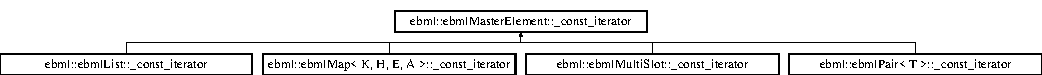
\includegraphics[height=1.007194cm]{classebml_1_1ebmlMasterElement_1_1__const__iterator}
\end{center}
\end{figure}
\subsection*{Public Member Functions}
\begin{DoxyCompactItemize}
\item 
virtual \mbox{\hyperlink{classebml_1_1ebmlMasterElement_1_1__const__iterator}{\+\_\+const\+\_\+iterator}} $\ast$ \mbox{\hyperlink{classebml_1_1ebmlMasterElement_1_1__const__iterator_a64a4853ad363358987eb6492579cd503}{copy}} () const =0
\item 
virtual \mbox{\hyperlink{namespaceebml_a2deef4e8071531b32e3533f1bf978917}{c\+\_\+ebml\+Element\+\_\+sp}} \mbox{\hyperlink{classebml_1_1ebmlMasterElement_1_1__const__iterator_aa3e5459826695a9043745fbbaea9cd47}{operator$\ast$}} () const =0
\item 
virtual \mbox{\hyperlink{classebml_1_1ebmlMasterElement_1_1__const__iterator}{\+\_\+const\+\_\+iterator}} \& \mbox{\hyperlink{classebml_1_1ebmlMasterElement_1_1__const__iterator_a439f540325443a3c3a3acdcd8df81553}{operator++}} ()=0
\item 
virtual \mbox{\hyperlink{classebml_1_1ebmlMasterElement_1_1__const__iterator}{\+\_\+const\+\_\+iterator}} \& \mbox{\hyperlink{classebml_1_1ebmlMasterElement_1_1__const__iterator_a102cf8b36c0d8184680ef15594bb59fb}{operator=}} (const \mbox{\hyperlink{classebml_1_1ebmlMasterElement_1_1__const__iterator}{\+\_\+const\+\_\+iterator}} \&)=0
\item 
virtual bool \mbox{\hyperlink{classebml_1_1ebmlMasterElement_1_1__const__iterator_a936395ed4c0c189a92927bfdf1e28586}{operator==}} (const \mbox{\hyperlink{classebml_1_1ebmlMasterElement_1_1__const__iterator}{\+\_\+const\+\_\+iterator}} \&) const =0
\item 
virtual bool \mbox{\hyperlink{classebml_1_1ebmlMasterElement_1_1__const__iterator_ac62d190e9da49236835f8219ec307d22}{operator!=}} (const \mbox{\hyperlink{classebml_1_1ebmlMasterElement_1_1__const__iterator}{\+\_\+const\+\_\+iterator}} \&) const =0
\item 
virtual \mbox{\hyperlink{classebml_1_1ebmlMasterElement_1_1__const__iterator_a6138f42b88ff06379d96a095a12ed136}{$\sim$\+\_\+const\+\_\+iterator}} ()
\end{DoxyCompactItemize}
\subsection*{Friends}
\begin{DoxyCompactItemize}
\item 
class \mbox{\hyperlink{classebml_1_1ebmlMasterElement_1_1__const__iterator_ad88e86cba72e9332a4693c1c6009b281}{ebml\+Master\+Element}}
\item 
class \mbox{\hyperlink{classebml_1_1ebmlMasterElement_1_1__const__iterator_a734affd0f736e2e4e03ab2cf8a9f9b26}{ebml\+Master\+Element\+::const\+\_\+iterator}}
\end{DoxyCompactItemize}


\subsection{Constructor \& Destructor Documentation}
\mbox{\Hypertarget{classebml_1_1ebmlMasterElement_1_1__const__iterator_a6138f42b88ff06379d96a095a12ed136}\label{classebml_1_1ebmlMasterElement_1_1__const__iterator_a6138f42b88ff06379d96a095a12ed136}} 
\index{ebml\+::ebml\+Master\+Element\+::\+\_\+const\+\_\+iterator@{ebml\+::ebml\+Master\+Element\+::\+\_\+const\+\_\+iterator}!````~\+\_\+const\+\_\+iterator@{$\sim$\+\_\+const\+\_\+iterator}}
\index{````~\+\_\+const\+\_\+iterator@{$\sim$\+\_\+const\+\_\+iterator}!ebml\+::ebml\+Master\+Element\+::\+\_\+const\+\_\+iterator@{ebml\+::ebml\+Master\+Element\+::\+\_\+const\+\_\+iterator}}
\subsubsection{\texorpdfstring{$\sim$\+\_\+const\+\_\+iterator()}{~\_const\_iterator()}}
{\footnotesize\ttfamily virtual ebml\+::ebml\+Master\+Element\+::\+\_\+const\+\_\+iterator\+::$\sim$\+\_\+const\+\_\+iterator (\begin{DoxyParamCaption}{ }\end{DoxyParamCaption})\hspace{0.3cm}{\ttfamily [inline]}, {\ttfamily [virtual]}}



Reimplemented in \mbox{\hyperlink{classebml_1_1ebmlMultiSlot_1_1__const__iterator_af518a921ebb2e2734b4d045d7d8be0f1}{ebml\+::ebml\+Multi\+Slot\+::\+\_\+const\+\_\+iterator}}, \mbox{\hyperlink{classebml_1_1ebmlMap_1_1__const__iterator_a4f230319e3c3dfa23ed8418d05ec8cc6}{ebml\+::ebml\+Map$<$ K, H, E, A $>$\+::\+\_\+const\+\_\+iterator}}, \mbox{\hyperlink{classebml_1_1ebmlPair_1_1__const__iterator_a2031860865632624af0ff271e7442089}{ebml\+::ebml\+Pair$<$ T $>$\+::\+\_\+const\+\_\+iterator}}, and \mbox{\hyperlink{classebml_1_1ebmlList_1_1__const__iterator_ad0a42056feeeb952125dcedd4eecb2a6}{ebml\+::ebml\+List\+::\+\_\+const\+\_\+iterator}}.



\subsection{Member Function Documentation}
\mbox{\Hypertarget{classebml_1_1ebmlMasterElement_1_1__const__iterator_a64a4853ad363358987eb6492579cd503}\label{classebml_1_1ebmlMasterElement_1_1__const__iterator_a64a4853ad363358987eb6492579cd503}} 
\index{ebml\+::ebml\+Master\+Element\+::\+\_\+const\+\_\+iterator@{ebml\+::ebml\+Master\+Element\+::\+\_\+const\+\_\+iterator}!copy@{copy}}
\index{copy@{copy}!ebml\+::ebml\+Master\+Element\+::\+\_\+const\+\_\+iterator@{ebml\+::ebml\+Master\+Element\+::\+\_\+const\+\_\+iterator}}
\subsubsection{\texorpdfstring{copy()}{copy()}}
{\footnotesize\ttfamily virtual \mbox{\hyperlink{classebml_1_1ebmlMasterElement_1_1__const__iterator}{\+\_\+const\+\_\+iterator}}$\ast$ ebml\+::ebml\+Master\+Element\+::\+\_\+const\+\_\+iterator\+::copy (\begin{DoxyParamCaption}{ }\end{DoxyParamCaption}) const\hspace{0.3cm}{\ttfamily [pure virtual]}}



Implemented in \mbox{\hyperlink{classebml_1_1ebmlMultiSlot_1_1__const__iterator_a412c3cc02df5d62c4a05be31aca752e5}{ebml\+::ebml\+Multi\+Slot\+::\+\_\+const\+\_\+iterator}}, \mbox{\hyperlink{classebml_1_1ebmlMap_1_1__const__iterator_af2bd75417ff0115d8bb53670ff8deaf2}{ebml\+::ebml\+Map$<$ K, H, E, A $>$\+::\+\_\+const\+\_\+iterator}}, \mbox{\hyperlink{classebml_1_1ebmlPair_1_1__const__iterator_a585b8bfa69c6746da17393207e599bca}{ebml\+::ebml\+Pair$<$ T $>$\+::\+\_\+const\+\_\+iterator}}, and \mbox{\hyperlink{classebml_1_1ebmlList_1_1__const__iterator_aae11488b46714c745cdd81d3fb75f57a}{ebml\+::ebml\+List\+::\+\_\+const\+\_\+iterator}}.

\mbox{\Hypertarget{classebml_1_1ebmlMasterElement_1_1__const__iterator_ac62d190e9da49236835f8219ec307d22}\label{classebml_1_1ebmlMasterElement_1_1__const__iterator_ac62d190e9da49236835f8219ec307d22}} 
\index{ebml\+::ebml\+Master\+Element\+::\+\_\+const\+\_\+iterator@{ebml\+::ebml\+Master\+Element\+::\+\_\+const\+\_\+iterator}!operator"!=@{operator"!=}}
\index{operator"!=@{operator"!=}!ebml\+::ebml\+Master\+Element\+::\+\_\+const\+\_\+iterator@{ebml\+::ebml\+Master\+Element\+::\+\_\+const\+\_\+iterator}}
\subsubsection{\texorpdfstring{operator"!=()}{operator!=()}}
{\footnotesize\ttfamily virtual bool ebml\+::ebml\+Master\+Element\+::\+\_\+const\+\_\+iterator\+::operator!= (\begin{DoxyParamCaption}\item[{const \mbox{\hyperlink{classebml_1_1ebmlMasterElement_1_1__const__iterator}{\+\_\+const\+\_\+iterator}} \&}]{ }\end{DoxyParamCaption}) const\hspace{0.3cm}{\ttfamily [pure virtual]}}



Implemented in \mbox{\hyperlink{classebml_1_1ebmlMultiSlot_1_1__const__iterator_a9a1c8df8a22d52ecb55de9f151f383e0}{ebml\+::ebml\+Multi\+Slot\+::\+\_\+const\+\_\+iterator}}, \mbox{\hyperlink{classebml_1_1ebmlMap_1_1__const__iterator_aa63b9e3fd20c1092792db91a25fb2b70}{ebml\+::ebml\+Map$<$ K, H, E, A $>$\+::\+\_\+const\+\_\+iterator}}, \mbox{\hyperlink{classebml_1_1ebmlPair_1_1__const__iterator_ae764d0a947293d8383d98c3105ce2fa7}{ebml\+::ebml\+Pair$<$ T $>$\+::\+\_\+const\+\_\+iterator}}, and \mbox{\hyperlink{classebml_1_1ebmlList_1_1__const__iterator_a21d545577f7b61b40ce961d5c9a83cce}{ebml\+::ebml\+List\+::\+\_\+const\+\_\+iterator}}.

\mbox{\Hypertarget{classebml_1_1ebmlMasterElement_1_1__const__iterator_aa3e5459826695a9043745fbbaea9cd47}\label{classebml_1_1ebmlMasterElement_1_1__const__iterator_aa3e5459826695a9043745fbbaea9cd47}} 
\index{ebml\+::ebml\+Master\+Element\+::\+\_\+const\+\_\+iterator@{ebml\+::ebml\+Master\+Element\+::\+\_\+const\+\_\+iterator}!operator$\ast$@{operator$\ast$}}
\index{operator$\ast$@{operator$\ast$}!ebml\+::ebml\+Master\+Element\+::\+\_\+const\+\_\+iterator@{ebml\+::ebml\+Master\+Element\+::\+\_\+const\+\_\+iterator}}
\subsubsection{\texorpdfstring{operator$\ast$()}{operator*()}}
{\footnotesize\ttfamily virtual \mbox{\hyperlink{namespaceebml_a2deef4e8071531b32e3533f1bf978917}{c\+\_\+ebml\+Element\+\_\+sp}} ebml\+::ebml\+Master\+Element\+::\+\_\+const\+\_\+iterator\+::operator$\ast$ (\begin{DoxyParamCaption}{ }\end{DoxyParamCaption}) const\hspace{0.3cm}{\ttfamily [pure virtual]}}



Implemented in \mbox{\hyperlink{classebml_1_1ebmlMultiSlot_1_1__const__iterator_ad4dfa7a3f08d535fe83c93c762009483}{ebml\+::ebml\+Multi\+Slot\+::\+\_\+const\+\_\+iterator}}, \mbox{\hyperlink{classebml_1_1ebmlMap_1_1__const__iterator_a7385fe1f7e51cdf2c4c538e9cc474583}{ebml\+::ebml\+Map$<$ K, H, E, A $>$\+::\+\_\+const\+\_\+iterator}}, \mbox{\hyperlink{classebml_1_1ebmlPair_1_1__const__iterator_ad5d24ee7d47113fbde6e2dc895b5b80a}{ebml\+::ebml\+Pair$<$ T $>$\+::\+\_\+const\+\_\+iterator}}, and \mbox{\hyperlink{classebml_1_1ebmlList_1_1__const__iterator_abc0aa1dd7a1d159c1a6f8c77e2736b80}{ebml\+::ebml\+List\+::\+\_\+const\+\_\+iterator}}.

\mbox{\Hypertarget{classebml_1_1ebmlMasterElement_1_1__const__iterator_a439f540325443a3c3a3acdcd8df81553}\label{classebml_1_1ebmlMasterElement_1_1__const__iterator_a439f540325443a3c3a3acdcd8df81553}} 
\index{ebml\+::ebml\+Master\+Element\+::\+\_\+const\+\_\+iterator@{ebml\+::ebml\+Master\+Element\+::\+\_\+const\+\_\+iterator}!operator++@{operator++}}
\index{operator++@{operator++}!ebml\+::ebml\+Master\+Element\+::\+\_\+const\+\_\+iterator@{ebml\+::ebml\+Master\+Element\+::\+\_\+const\+\_\+iterator}}
\subsubsection{\texorpdfstring{operator++()}{operator++()}}
{\footnotesize\ttfamily virtual \mbox{\hyperlink{classebml_1_1ebmlMasterElement_1_1__const__iterator}{\+\_\+const\+\_\+iterator}}\& ebml\+::ebml\+Master\+Element\+::\+\_\+const\+\_\+iterator\+::operator++ (\begin{DoxyParamCaption}{ }\end{DoxyParamCaption})\hspace{0.3cm}{\ttfamily [pure virtual]}}



Implemented in \mbox{\hyperlink{classebml_1_1ebmlMultiSlot_1_1__const__iterator_a4d9425007a96cb4803ef3cff5bf88e00}{ebml\+::ebml\+Multi\+Slot\+::\+\_\+const\+\_\+iterator}}, \mbox{\hyperlink{classebml_1_1ebmlMap_1_1__const__iterator_a7a58190879091815afc606e295afd1cf}{ebml\+::ebml\+Map$<$ K, H, E, A $>$\+::\+\_\+const\+\_\+iterator}}, \mbox{\hyperlink{classebml_1_1ebmlPair_1_1__const__iterator_a504a93a5fa6b77f8604016c50957ef0c}{ebml\+::ebml\+Pair$<$ T $>$\+::\+\_\+const\+\_\+iterator}}, and \mbox{\hyperlink{classebml_1_1ebmlList_1_1__const__iterator_a20f27b727326834e8b2a1c1dd66ffbce}{ebml\+::ebml\+List\+::\+\_\+const\+\_\+iterator}}.

\mbox{\Hypertarget{classebml_1_1ebmlMasterElement_1_1__const__iterator_a102cf8b36c0d8184680ef15594bb59fb}\label{classebml_1_1ebmlMasterElement_1_1__const__iterator_a102cf8b36c0d8184680ef15594bb59fb}} 
\index{ebml\+::ebml\+Master\+Element\+::\+\_\+const\+\_\+iterator@{ebml\+::ebml\+Master\+Element\+::\+\_\+const\+\_\+iterator}!operator=@{operator=}}
\index{operator=@{operator=}!ebml\+::ebml\+Master\+Element\+::\+\_\+const\+\_\+iterator@{ebml\+::ebml\+Master\+Element\+::\+\_\+const\+\_\+iterator}}
\subsubsection{\texorpdfstring{operator=()}{operator=()}}
{\footnotesize\ttfamily virtual \mbox{\hyperlink{classebml_1_1ebmlMasterElement_1_1__const__iterator}{\+\_\+const\+\_\+iterator}}\& ebml\+::ebml\+Master\+Element\+::\+\_\+const\+\_\+iterator\+::operator= (\begin{DoxyParamCaption}\item[{const \mbox{\hyperlink{classebml_1_1ebmlMasterElement_1_1__const__iterator}{\+\_\+const\+\_\+iterator}} \&}]{ }\end{DoxyParamCaption})\hspace{0.3cm}{\ttfamily [pure virtual]}}



Implemented in \mbox{\hyperlink{classebml_1_1ebmlMultiSlot_1_1__const__iterator_a6e2de45285786f1045fef8be51974b0b}{ebml\+::ebml\+Multi\+Slot\+::\+\_\+const\+\_\+iterator}}, \mbox{\hyperlink{classebml_1_1ebmlMap_1_1__const__iterator_a641afb65930e85882c6397d2f0930604}{ebml\+::ebml\+Map$<$ K, H, E, A $>$\+::\+\_\+const\+\_\+iterator}}, \mbox{\hyperlink{classebml_1_1ebmlPair_1_1__const__iterator_a84535e268f7488e9acff8e5d35de4f38}{ebml\+::ebml\+Pair$<$ T $>$\+::\+\_\+const\+\_\+iterator}}, and \mbox{\hyperlink{classebml_1_1ebmlList_1_1__const__iterator_a10b96fa207ad1c24cb2374c1ee417646}{ebml\+::ebml\+List\+::\+\_\+const\+\_\+iterator}}.

\mbox{\Hypertarget{classebml_1_1ebmlMasterElement_1_1__const__iterator_a936395ed4c0c189a92927bfdf1e28586}\label{classebml_1_1ebmlMasterElement_1_1__const__iterator_a936395ed4c0c189a92927bfdf1e28586}} 
\index{ebml\+::ebml\+Master\+Element\+::\+\_\+const\+\_\+iterator@{ebml\+::ebml\+Master\+Element\+::\+\_\+const\+\_\+iterator}!operator==@{operator==}}
\index{operator==@{operator==}!ebml\+::ebml\+Master\+Element\+::\+\_\+const\+\_\+iterator@{ebml\+::ebml\+Master\+Element\+::\+\_\+const\+\_\+iterator}}
\subsubsection{\texorpdfstring{operator==()}{operator==()}}
{\footnotesize\ttfamily virtual bool ebml\+::ebml\+Master\+Element\+::\+\_\+const\+\_\+iterator\+::operator== (\begin{DoxyParamCaption}\item[{const \mbox{\hyperlink{classebml_1_1ebmlMasterElement_1_1__const__iterator}{\+\_\+const\+\_\+iterator}} \&}]{ }\end{DoxyParamCaption}) const\hspace{0.3cm}{\ttfamily [pure virtual]}}



Implemented in \mbox{\hyperlink{classebml_1_1ebmlMultiSlot_1_1__const__iterator_a874e71d4f6d86e1213c8381ec20f3069}{ebml\+::ebml\+Multi\+Slot\+::\+\_\+const\+\_\+iterator}}, \mbox{\hyperlink{classebml_1_1ebmlMap_1_1__const__iterator_aa0b4af1c5b7d8bdb26def33c2a329371}{ebml\+::ebml\+Map$<$ K, H, E, A $>$\+::\+\_\+const\+\_\+iterator}}, \mbox{\hyperlink{classebml_1_1ebmlPair_1_1__const__iterator_a2b9f927f8b57e7db13693581d6592e1e}{ebml\+::ebml\+Pair$<$ T $>$\+::\+\_\+const\+\_\+iterator}}, and \mbox{\hyperlink{classebml_1_1ebmlList_1_1__const__iterator_af5249ca7b9ac67296b1e92ffa804bce5}{ebml\+::ebml\+List\+::\+\_\+const\+\_\+iterator}}.



\subsection{Friends And Related Function Documentation}
\mbox{\Hypertarget{classebml_1_1ebmlMasterElement_1_1__const__iterator_ad88e86cba72e9332a4693c1c6009b281}\label{classebml_1_1ebmlMasterElement_1_1__const__iterator_ad88e86cba72e9332a4693c1c6009b281}} 
\index{ebml\+::ebml\+Master\+Element\+::\+\_\+const\+\_\+iterator@{ebml\+::ebml\+Master\+Element\+::\+\_\+const\+\_\+iterator}!ebml\+Master\+Element@{ebml\+Master\+Element}}
\index{ebml\+Master\+Element@{ebml\+Master\+Element}!ebml\+::ebml\+Master\+Element\+::\+\_\+const\+\_\+iterator@{ebml\+::ebml\+Master\+Element\+::\+\_\+const\+\_\+iterator}}
\subsubsection{\texorpdfstring{ebml\+Master\+Element}{ebmlMasterElement}}
{\footnotesize\ttfamily friend class \mbox{\hyperlink{classebml_1_1ebmlMasterElement}{ebml\+Master\+Element}}\hspace{0.3cm}{\ttfamily [friend]}}

\mbox{\Hypertarget{classebml_1_1ebmlMasterElement_1_1__const__iterator_a734affd0f736e2e4e03ab2cf8a9f9b26}\label{classebml_1_1ebmlMasterElement_1_1__const__iterator_a734affd0f736e2e4e03ab2cf8a9f9b26}} 
\index{ebml\+::ebml\+Master\+Element\+::\+\_\+const\+\_\+iterator@{ebml\+::ebml\+Master\+Element\+::\+\_\+const\+\_\+iterator}!ebml\+Master\+Element\+::const\+\_\+iterator@{ebml\+Master\+Element\+::const\+\_\+iterator}}
\index{ebml\+Master\+Element\+::const\+\_\+iterator@{ebml\+Master\+Element\+::const\+\_\+iterator}!ebml\+::ebml\+Master\+Element\+::\+\_\+const\+\_\+iterator@{ebml\+::ebml\+Master\+Element\+::\+\_\+const\+\_\+iterator}}
\subsubsection{\texorpdfstring{ebml\+Master\+Element\+::const\+\_\+iterator}{ebmlMasterElement::const\_iterator}}
{\footnotesize\ttfamily friend class \mbox{\hyperlink{classebml_1_1ebmlMasterElement_1_1const__iterator}{ebml\+Master\+Element\+::const\+\_\+iterator}}\hspace{0.3cm}{\ttfamily [friend]}}



The documentation for this class was generated from the following file\+:\begin{DoxyCompactItemize}
\item 
include/libebml\+\_\+ng/masterelement/\mbox{\hyperlink{base_8h}{base.\+h}}\end{DoxyCompactItemize}

\hypertarget{classebml_1_1ebmlList_1_1__const__iterator}{}\section{ebml\+:\+:ebml\+List\+:\+:\+\_\+const\+\_\+iterator Class Reference}
\label{classebml_1_1ebmlList_1_1__const__iterator}\index{ebml\+::ebml\+List\+::\+\_\+const\+\_\+iterator@{ebml\+::ebml\+List\+::\+\_\+const\+\_\+iterator}}


{\ttfamily \#include $<$list.\+h$>$}

Inheritance diagram for ebml\+:\+:ebml\+List\+:\+:\+\_\+const\+\_\+iterator\+:\begin{figure}[H]
\begin{center}
\leavevmode
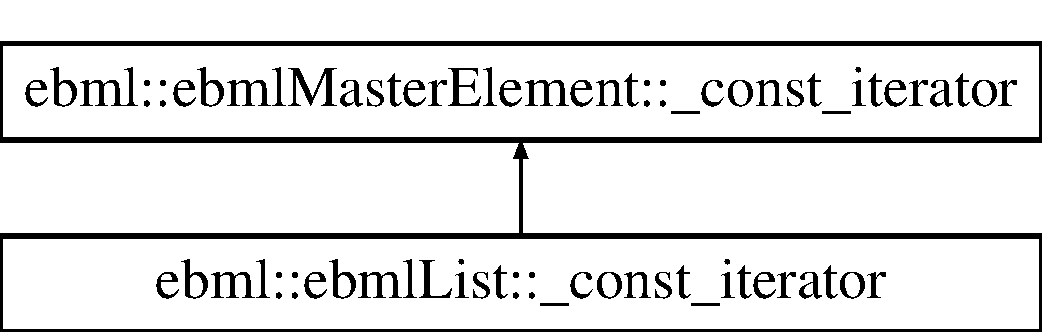
\includegraphics[height=2.000000cm]{classebml_1_1ebmlList_1_1__const__iterator}
\end{center}
\end{figure}
\subsection*{Public Member Functions}
\begin{DoxyCompactItemize}
\item 
\mbox{\hyperlink{classebml_1_1ebmlList_1_1__const__iterator_a2e4df37bf8485e7517498683f5ab5ca6}{\+\_\+const\+\_\+iterator}} ()
\item 
virtual \mbox{\hyperlink{classebml_1_1ebmlList_1_1__const__iterator_ad0a42056feeeb952125dcedd4eecb2a6}{$\sim$\+\_\+const\+\_\+iterator}} ()
\item 
\mbox{\hyperlink{classebml_1_1ebmlMasterElement_1_1__const__iterator}{ebml\+Master\+Element\+::\+\_\+const\+\_\+iterator}} $\ast$ \mbox{\hyperlink{classebml_1_1ebmlList_1_1__const__iterator_aae11488b46714c745cdd81d3fb75f57a}{copy}} () const
\item 
\mbox{\hyperlink{namespaceebml_a2deef4e8071531b32e3533f1bf978917}{c\+\_\+ebml\+Element\+\_\+sp}} \mbox{\hyperlink{classebml_1_1ebmlList_1_1__const__iterator_abc0aa1dd7a1d159c1a6f8c77e2736b80}{operator$\ast$}} () const
\item 
\mbox{\hyperlink{classebml_1_1ebmlMasterElement_1_1__const__iterator}{ebml\+Master\+Element\+::\+\_\+const\+\_\+iterator}} \& \mbox{\hyperlink{classebml_1_1ebmlList_1_1__const__iterator_a20f27b727326834e8b2a1c1dd66ffbce}{operator++}} ()
\item 
\mbox{\hyperlink{classebml_1_1ebmlMasterElement_1_1__const__iterator}{ebml\+Master\+Element\+::\+\_\+const\+\_\+iterator}} \& \mbox{\hyperlink{classebml_1_1ebmlList_1_1__const__iterator_a10b96fa207ad1c24cb2374c1ee417646}{operator=}} (const \mbox{\hyperlink{classebml_1_1ebmlMasterElement_1_1__const__iterator}{ebml\+Master\+Element\+::\+\_\+const\+\_\+iterator}} \&)
\item 
bool \mbox{\hyperlink{classebml_1_1ebmlList_1_1__const__iterator_af5249ca7b9ac67296b1e92ffa804bce5}{operator==}} (const \mbox{\hyperlink{classebml_1_1ebmlMasterElement_1_1__const__iterator}{ebml\+Master\+Element\+::\+\_\+const\+\_\+iterator}} \&) const
\item 
bool \mbox{\hyperlink{classebml_1_1ebmlList_1_1__const__iterator_a21d545577f7b61b40ce961d5c9a83cce}{operator!=}} (const \mbox{\hyperlink{classebml_1_1ebmlMasterElement_1_1__const__iterator}{ebml\+Master\+Element\+::\+\_\+const\+\_\+iterator}} \&) const
\end{DoxyCompactItemize}
\subsection*{Protected Member Functions}
\begin{DoxyCompactItemize}
\item 
\mbox{\hyperlink{classebml_1_1ebmlList_1_1__const__iterator_aae58bee847fdcb8173e9b1eb220c7609}{\+\_\+const\+\_\+iterator}} (const \mbox{\hyperlink{namespaceebml_a2deef4e8071531b32e3533f1bf978917}{c\+\_\+ebml\+Element\+\_\+sp}} \&elem, const std\+::vector$<$ \mbox{\hyperlink{namespaceebml_adad533b7705a16bb360fe56380c5e7be}{ebml\+Element\+\_\+sp}} $>$\+::const\+\_\+iterator \&iter)
\end{DoxyCompactItemize}
\subsection*{Friends}
\begin{DoxyCompactItemize}
\item 
class \mbox{\hyperlink{classebml_1_1ebmlList_1_1__const__iterator_af371b14231393d2eef62cb562cdd6e2d}{ebml\+List}}
\item 
class \mbox{\hyperlink{classebml_1_1ebmlList_1_1__const__iterator_a734affd0f736e2e4e03ab2cf8a9f9b26}{ebml\+Master\+Element\+::const\+\_\+iterator}}
\end{DoxyCompactItemize}


\subsection{Constructor \& Destructor Documentation}
\mbox{\Hypertarget{classebml_1_1ebmlList_1_1__const__iterator_aae58bee847fdcb8173e9b1eb220c7609}\label{classebml_1_1ebmlList_1_1__const__iterator_aae58bee847fdcb8173e9b1eb220c7609}} 
\index{ebml\+::ebml\+List\+::\+\_\+const\+\_\+iterator@{ebml\+::ebml\+List\+::\+\_\+const\+\_\+iterator}!\+\_\+const\+\_\+iterator@{\+\_\+const\+\_\+iterator}}
\index{\+\_\+const\+\_\+iterator@{\+\_\+const\+\_\+iterator}!ebml\+::ebml\+List\+::\+\_\+const\+\_\+iterator@{ebml\+::ebml\+List\+::\+\_\+const\+\_\+iterator}}
\subsubsection{\texorpdfstring{\+\_\+const\+\_\+iterator()}{\_const\_iterator()}\hspace{0.1cm}{\footnotesize\ttfamily [1/2]}}
{\footnotesize\ttfamily ebml\+::ebml\+List\+::\+\_\+const\+\_\+iterator\+::\+\_\+const\+\_\+iterator (\begin{DoxyParamCaption}\item[{const \mbox{\hyperlink{namespaceebml_a2deef4e8071531b32e3533f1bf978917}{c\+\_\+ebml\+Element\+\_\+sp}} \&}]{elem,  }\item[{const std\+::vector$<$ \mbox{\hyperlink{namespaceebml_adad533b7705a16bb360fe56380c5e7be}{ebml\+Element\+\_\+sp}} $>$\+::const\+\_\+iterator \&}]{iter }\end{DoxyParamCaption})\hspace{0.3cm}{\ttfamily [protected]}}

\mbox{\Hypertarget{classebml_1_1ebmlList_1_1__const__iterator_a2e4df37bf8485e7517498683f5ab5ca6}\label{classebml_1_1ebmlList_1_1__const__iterator_a2e4df37bf8485e7517498683f5ab5ca6}} 
\index{ebml\+::ebml\+List\+::\+\_\+const\+\_\+iterator@{ebml\+::ebml\+List\+::\+\_\+const\+\_\+iterator}!\+\_\+const\+\_\+iterator@{\+\_\+const\+\_\+iterator}}
\index{\+\_\+const\+\_\+iterator@{\+\_\+const\+\_\+iterator}!ebml\+::ebml\+List\+::\+\_\+const\+\_\+iterator@{ebml\+::ebml\+List\+::\+\_\+const\+\_\+iterator}}
\subsubsection{\texorpdfstring{\+\_\+const\+\_\+iterator()}{\_const\_iterator()}\hspace{0.1cm}{\footnotesize\ttfamily [2/2]}}
{\footnotesize\ttfamily ebml\+::ebml\+List\+::\+\_\+const\+\_\+iterator\+::\+\_\+const\+\_\+iterator (\begin{DoxyParamCaption}{ }\end{DoxyParamCaption})}

\mbox{\Hypertarget{classebml_1_1ebmlList_1_1__const__iterator_ad0a42056feeeb952125dcedd4eecb2a6}\label{classebml_1_1ebmlList_1_1__const__iterator_ad0a42056feeeb952125dcedd4eecb2a6}} 
\index{ebml\+::ebml\+List\+::\+\_\+const\+\_\+iterator@{ebml\+::ebml\+List\+::\+\_\+const\+\_\+iterator}!````~\+\_\+const\+\_\+iterator@{$\sim$\+\_\+const\+\_\+iterator}}
\index{````~\+\_\+const\+\_\+iterator@{$\sim$\+\_\+const\+\_\+iterator}!ebml\+::ebml\+List\+::\+\_\+const\+\_\+iterator@{ebml\+::ebml\+List\+::\+\_\+const\+\_\+iterator}}
\subsubsection{\texorpdfstring{$\sim$\+\_\+const\+\_\+iterator()}{~\_const\_iterator()}}
{\footnotesize\ttfamily virtual ebml\+::ebml\+List\+::\+\_\+const\+\_\+iterator\+::$\sim$\+\_\+const\+\_\+iterator (\begin{DoxyParamCaption}{ }\end{DoxyParamCaption})\hspace{0.3cm}{\ttfamily [virtual]}}



Reimplemented from \mbox{\hyperlink{classebml_1_1ebmlMasterElement_1_1__const__iterator_a6138f42b88ff06379d96a095a12ed136}{ebml\+::ebml\+Master\+Element\+::\+\_\+const\+\_\+iterator}}.



\subsection{Member Function Documentation}
\mbox{\Hypertarget{classebml_1_1ebmlList_1_1__const__iterator_aae11488b46714c745cdd81d3fb75f57a}\label{classebml_1_1ebmlList_1_1__const__iterator_aae11488b46714c745cdd81d3fb75f57a}} 
\index{ebml\+::ebml\+List\+::\+\_\+const\+\_\+iterator@{ebml\+::ebml\+List\+::\+\_\+const\+\_\+iterator}!copy@{copy}}
\index{copy@{copy}!ebml\+::ebml\+List\+::\+\_\+const\+\_\+iterator@{ebml\+::ebml\+List\+::\+\_\+const\+\_\+iterator}}
\subsubsection{\texorpdfstring{copy()}{copy()}}
{\footnotesize\ttfamily \mbox{\hyperlink{classebml_1_1ebmlMasterElement_1_1__const__iterator}{ebml\+Master\+Element\+::\+\_\+const\+\_\+iterator}}$\ast$ ebml\+::ebml\+List\+::\+\_\+const\+\_\+iterator\+::copy (\begin{DoxyParamCaption}{ }\end{DoxyParamCaption}) const\hspace{0.3cm}{\ttfamily [virtual]}}



Implements \mbox{\hyperlink{classebml_1_1ebmlMasterElement_1_1__const__iterator_a64a4853ad363358987eb6492579cd503}{ebml\+::ebml\+Master\+Element\+::\+\_\+const\+\_\+iterator}}.

\mbox{\Hypertarget{classebml_1_1ebmlList_1_1__const__iterator_a21d545577f7b61b40ce961d5c9a83cce}\label{classebml_1_1ebmlList_1_1__const__iterator_a21d545577f7b61b40ce961d5c9a83cce}} 
\index{ebml\+::ebml\+List\+::\+\_\+const\+\_\+iterator@{ebml\+::ebml\+List\+::\+\_\+const\+\_\+iterator}!operator"!=@{operator"!=}}
\index{operator"!=@{operator"!=}!ebml\+::ebml\+List\+::\+\_\+const\+\_\+iterator@{ebml\+::ebml\+List\+::\+\_\+const\+\_\+iterator}}
\subsubsection{\texorpdfstring{operator"!=()}{operator!=()}}
{\footnotesize\ttfamily bool ebml\+::ebml\+List\+::\+\_\+const\+\_\+iterator\+::operator!= (\begin{DoxyParamCaption}\item[{const \mbox{\hyperlink{classebml_1_1ebmlMasterElement_1_1__const__iterator}{ebml\+Master\+Element\+::\+\_\+const\+\_\+iterator}} \&}]{ }\end{DoxyParamCaption}) const\hspace{0.3cm}{\ttfamily [virtual]}}



Implements \mbox{\hyperlink{classebml_1_1ebmlMasterElement_1_1__const__iterator_ac62d190e9da49236835f8219ec307d22}{ebml\+::ebml\+Master\+Element\+::\+\_\+const\+\_\+iterator}}.

\mbox{\Hypertarget{classebml_1_1ebmlList_1_1__const__iterator_abc0aa1dd7a1d159c1a6f8c77e2736b80}\label{classebml_1_1ebmlList_1_1__const__iterator_abc0aa1dd7a1d159c1a6f8c77e2736b80}} 
\index{ebml\+::ebml\+List\+::\+\_\+const\+\_\+iterator@{ebml\+::ebml\+List\+::\+\_\+const\+\_\+iterator}!operator$\ast$@{operator$\ast$}}
\index{operator$\ast$@{operator$\ast$}!ebml\+::ebml\+List\+::\+\_\+const\+\_\+iterator@{ebml\+::ebml\+List\+::\+\_\+const\+\_\+iterator}}
\subsubsection{\texorpdfstring{operator$\ast$()}{operator*()}}
{\footnotesize\ttfamily \mbox{\hyperlink{namespaceebml_a2deef4e8071531b32e3533f1bf978917}{c\+\_\+ebml\+Element\+\_\+sp}} ebml\+::ebml\+List\+::\+\_\+const\+\_\+iterator\+::operator$\ast$ (\begin{DoxyParamCaption}{ }\end{DoxyParamCaption}) const\hspace{0.3cm}{\ttfamily [virtual]}}



Implements \mbox{\hyperlink{classebml_1_1ebmlMasterElement_1_1__const__iterator_aa3e5459826695a9043745fbbaea9cd47}{ebml\+::ebml\+Master\+Element\+::\+\_\+const\+\_\+iterator}}.

\mbox{\Hypertarget{classebml_1_1ebmlList_1_1__const__iterator_a20f27b727326834e8b2a1c1dd66ffbce}\label{classebml_1_1ebmlList_1_1__const__iterator_a20f27b727326834e8b2a1c1dd66ffbce}} 
\index{ebml\+::ebml\+List\+::\+\_\+const\+\_\+iterator@{ebml\+::ebml\+List\+::\+\_\+const\+\_\+iterator}!operator++@{operator++}}
\index{operator++@{operator++}!ebml\+::ebml\+List\+::\+\_\+const\+\_\+iterator@{ebml\+::ebml\+List\+::\+\_\+const\+\_\+iterator}}
\subsubsection{\texorpdfstring{operator++()}{operator++()}}
{\footnotesize\ttfamily \mbox{\hyperlink{classebml_1_1ebmlMasterElement_1_1__const__iterator}{ebml\+Master\+Element\+::\+\_\+const\+\_\+iterator}}\& ebml\+::ebml\+List\+::\+\_\+const\+\_\+iterator\+::operator++ (\begin{DoxyParamCaption}{ }\end{DoxyParamCaption})\hspace{0.3cm}{\ttfamily [virtual]}}



Implements \mbox{\hyperlink{classebml_1_1ebmlMasterElement_1_1__const__iterator_a439f540325443a3c3a3acdcd8df81553}{ebml\+::ebml\+Master\+Element\+::\+\_\+const\+\_\+iterator}}.

\mbox{\Hypertarget{classebml_1_1ebmlList_1_1__const__iterator_a10b96fa207ad1c24cb2374c1ee417646}\label{classebml_1_1ebmlList_1_1__const__iterator_a10b96fa207ad1c24cb2374c1ee417646}} 
\index{ebml\+::ebml\+List\+::\+\_\+const\+\_\+iterator@{ebml\+::ebml\+List\+::\+\_\+const\+\_\+iterator}!operator=@{operator=}}
\index{operator=@{operator=}!ebml\+::ebml\+List\+::\+\_\+const\+\_\+iterator@{ebml\+::ebml\+List\+::\+\_\+const\+\_\+iterator}}
\subsubsection{\texorpdfstring{operator=()}{operator=()}}
{\footnotesize\ttfamily \mbox{\hyperlink{classebml_1_1ebmlMasterElement_1_1__const__iterator}{ebml\+Master\+Element\+::\+\_\+const\+\_\+iterator}}\& ebml\+::ebml\+List\+::\+\_\+const\+\_\+iterator\+::operator= (\begin{DoxyParamCaption}\item[{const \mbox{\hyperlink{classebml_1_1ebmlMasterElement_1_1__const__iterator}{ebml\+Master\+Element\+::\+\_\+const\+\_\+iterator}} \&}]{ }\end{DoxyParamCaption})\hspace{0.3cm}{\ttfamily [virtual]}}



Implements \mbox{\hyperlink{classebml_1_1ebmlMasterElement_1_1__const__iterator_a102cf8b36c0d8184680ef15594bb59fb}{ebml\+::ebml\+Master\+Element\+::\+\_\+const\+\_\+iterator}}.

\mbox{\Hypertarget{classebml_1_1ebmlList_1_1__const__iterator_af5249ca7b9ac67296b1e92ffa804bce5}\label{classebml_1_1ebmlList_1_1__const__iterator_af5249ca7b9ac67296b1e92ffa804bce5}} 
\index{ebml\+::ebml\+List\+::\+\_\+const\+\_\+iterator@{ebml\+::ebml\+List\+::\+\_\+const\+\_\+iterator}!operator==@{operator==}}
\index{operator==@{operator==}!ebml\+::ebml\+List\+::\+\_\+const\+\_\+iterator@{ebml\+::ebml\+List\+::\+\_\+const\+\_\+iterator}}
\subsubsection{\texorpdfstring{operator==()}{operator==()}}
{\footnotesize\ttfamily bool ebml\+::ebml\+List\+::\+\_\+const\+\_\+iterator\+::operator== (\begin{DoxyParamCaption}\item[{const \mbox{\hyperlink{classebml_1_1ebmlMasterElement_1_1__const__iterator}{ebml\+Master\+Element\+::\+\_\+const\+\_\+iterator}} \&}]{ }\end{DoxyParamCaption}) const\hspace{0.3cm}{\ttfamily [virtual]}}



Implements \mbox{\hyperlink{classebml_1_1ebmlMasterElement_1_1__const__iterator_a936395ed4c0c189a92927bfdf1e28586}{ebml\+::ebml\+Master\+Element\+::\+\_\+const\+\_\+iterator}}.



\subsection{Friends And Related Function Documentation}
\mbox{\Hypertarget{classebml_1_1ebmlList_1_1__const__iterator_af371b14231393d2eef62cb562cdd6e2d}\label{classebml_1_1ebmlList_1_1__const__iterator_af371b14231393d2eef62cb562cdd6e2d}} 
\index{ebml\+::ebml\+List\+::\+\_\+const\+\_\+iterator@{ebml\+::ebml\+List\+::\+\_\+const\+\_\+iterator}!ebml\+List@{ebml\+List}}
\index{ebml\+List@{ebml\+List}!ebml\+::ebml\+List\+::\+\_\+const\+\_\+iterator@{ebml\+::ebml\+List\+::\+\_\+const\+\_\+iterator}}
\subsubsection{\texorpdfstring{ebml\+List}{ebmlList}}
{\footnotesize\ttfamily friend class \mbox{\hyperlink{classebml_1_1ebmlList}{ebml\+List}}\hspace{0.3cm}{\ttfamily [friend]}}

\mbox{\Hypertarget{classebml_1_1ebmlList_1_1__const__iterator_a734affd0f736e2e4e03ab2cf8a9f9b26}\label{classebml_1_1ebmlList_1_1__const__iterator_a734affd0f736e2e4e03ab2cf8a9f9b26}} 
\index{ebml\+::ebml\+List\+::\+\_\+const\+\_\+iterator@{ebml\+::ebml\+List\+::\+\_\+const\+\_\+iterator}!ebml\+Master\+Element\+::const\+\_\+iterator@{ebml\+Master\+Element\+::const\+\_\+iterator}}
\index{ebml\+Master\+Element\+::const\+\_\+iterator@{ebml\+Master\+Element\+::const\+\_\+iterator}!ebml\+::ebml\+List\+::\+\_\+const\+\_\+iterator@{ebml\+::ebml\+List\+::\+\_\+const\+\_\+iterator}}
\subsubsection{\texorpdfstring{ebml\+Master\+Element\+::const\+\_\+iterator}{ebmlMasterElement::const\_iterator}}
{\footnotesize\ttfamily friend class \mbox{\hyperlink{classebml_1_1ebmlMasterElement_1_1const__iterator}{ebml\+Master\+Element\+::const\+\_\+iterator}}\hspace{0.3cm}{\ttfamily [friend]}}



The documentation for this class was generated from the following file\+:\begin{DoxyCompactItemize}
\item 
include/libebml\+\_\+ng/masterelement/\mbox{\hyperlink{list_8h}{list.\+h}}\end{DoxyCompactItemize}

\hypertarget{classebml_1_1ebmlPair_1_1__const__iterator}{}\section{ebml\+:\+:ebml\+Pair$<$ T $>$\+:\+:\+\_\+const\+\_\+iterator Class Reference}
\label{classebml_1_1ebmlPair_1_1__const__iterator}\index{ebml\+::ebml\+Pair$<$ T $>$\+::\+\_\+const\+\_\+iterator@{ebml\+::ebml\+Pair$<$ T $>$\+::\+\_\+const\+\_\+iterator}}


{\ttfamily \#include $<$map.\+h$>$}

Inheritance diagram for ebml\+:\+:ebml\+Pair$<$ T $>$\+:\+:\+\_\+const\+\_\+iterator\+:\begin{figure}[H]
\begin{center}
\leavevmode
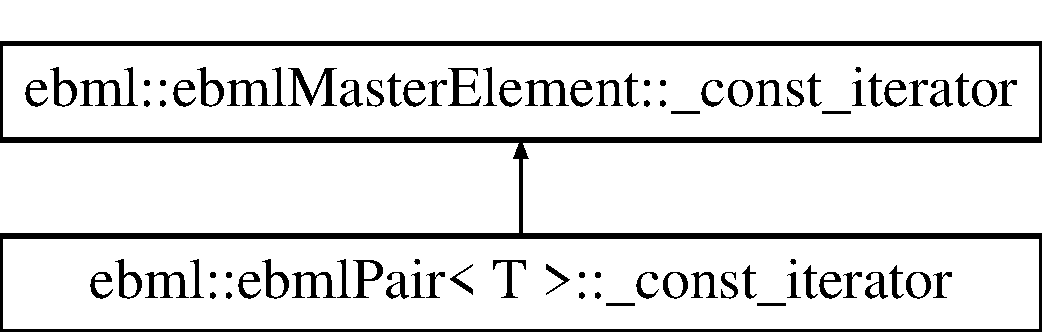
\includegraphics[height=2.000000cm]{classebml_1_1ebmlPair_1_1__const__iterator}
\end{center}
\end{figure}
\subsection*{Public Member Functions}
\begin{DoxyCompactItemize}
\item 
\mbox{\hyperlink{classebml_1_1ebmlPair_1_1__const__iterator_a4e541f74f5e9b207f07c843eba7dbf89}{\+\_\+const\+\_\+iterator}} ()
\item 
virtual \mbox{\hyperlink{classebml_1_1ebmlPair_1_1__const__iterator_a2031860865632624af0ff271e7442089}{$\sim$\+\_\+const\+\_\+iterator}} ()
\item 
\mbox{\hyperlink{classebml_1_1ebmlMasterElement_1_1__const__iterator}{ebml\+Master\+Element\+::\+\_\+const\+\_\+iterator}} $\ast$ \mbox{\hyperlink{classebml_1_1ebmlPair_1_1__const__iterator_a585b8bfa69c6746da17393207e599bca}{copy}} () const
\item 
\mbox{\hyperlink{namespaceebml_a2deef4e8071531b32e3533f1bf978917}{c\+\_\+ebml\+Element\+\_\+sp}} \mbox{\hyperlink{classebml_1_1ebmlPair_1_1__const__iterator_ad5d24ee7d47113fbde6e2dc895b5b80a}{operator$\ast$}} () const
\item 
\mbox{\hyperlink{classebml_1_1ebmlMasterElement_1_1__const__iterator}{ebml\+Master\+Element\+::\+\_\+const\+\_\+iterator}} \& \mbox{\hyperlink{classebml_1_1ebmlPair_1_1__const__iterator_a504a93a5fa6b77f8604016c50957ef0c}{operator++}} ()
\item 
\mbox{\hyperlink{classebml_1_1ebmlMasterElement_1_1__const__iterator}{ebml\+Master\+Element\+::\+\_\+const\+\_\+iterator}} \& \mbox{\hyperlink{classebml_1_1ebmlPair_1_1__const__iterator_a84535e268f7488e9acff8e5d35de4f38}{operator=}} (const \mbox{\hyperlink{classebml_1_1ebmlMasterElement_1_1__const__iterator}{ebml\+Master\+Element\+::\+\_\+const\+\_\+iterator}} \&)
\item 
bool \mbox{\hyperlink{classebml_1_1ebmlPair_1_1__const__iterator_a2b9f927f8b57e7db13693581d6592e1e}{operator==}} (const \mbox{\hyperlink{classebml_1_1ebmlMasterElement_1_1__const__iterator}{ebml\+Master\+Element\+::\+\_\+const\+\_\+iterator}} \&) const
\item 
bool \mbox{\hyperlink{classebml_1_1ebmlPair_1_1__const__iterator_ae764d0a947293d8383d98c3105ce2fa7}{operator!=}} (const \mbox{\hyperlink{classebml_1_1ebmlMasterElement_1_1__const__iterator}{ebml\+Master\+Element\+::\+\_\+const\+\_\+iterator}} \&) const
\end{DoxyCompactItemize}
\subsection*{Protected Member Functions}
\begin{DoxyCompactItemize}
\item 
\mbox{\hyperlink{classebml_1_1ebmlPair_1_1__const__iterator_af56c2752b5cc334ec40e380d6f5a3301}{\+\_\+const\+\_\+iterator}} (const \mbox{\hyperlink{namespaceebml_a9c804317d5b51ef8844bdffe5e8cb4b3}{c\+\_\+ebml\+Pair\+\_\+sp}}$<$ T $>$ \&elem, unsigned char pos)
\item 
\mbox{\hyperlink{classebml_1_1ebmlPair_1_1__const__iterator_a703a5a75fe4cd7809ab31cdd1b3cb54b}{\+\_\+const\+\_\+iterator}} (\mbox{\hyperlink{namespaceebml_a9c804317d5b51ef8844bdffe5e8cb4b3}{c\+\_\+ebml\+Pair\+\_\+sp}}$<$ T $>$ \&\&elem, unsigned char pos)
\end{DoxyCompactItemize}
\subsection*{Friends}
\begin{DoxyCompactItemize}
\item 
class \mbox{\hyperlink{classebml_1_1ebmlPair_1_1__const__iterator_ad1db4b5395f31070d1be2d251ee85e02}{ebml\+Pair$<$ T $>$}}
\item 
class \mbox{\hyperlink{classebml_1_1ebmlPair_1_1__const__iterator_a734affd0f736e2e4e03ab2cf8a9f9b26}{ebml\+Master\+Element\+::const\+\_\+iterator}}
\end{DoxyCompactItemize}


\subsection{Constructor \& Destructor Documentation}
\mbox{\Hypertarget{classebml_1_1ebmlPair_1_1__const__iterator_af56c2752b5cc334ec40e380d6f5a3301}\label{classebml_1_1ebmlPair_1_1__const__iterator_af56c2752b5cc334ec40e380d6f5a3301}} 
\index{ebml\+::ebml\+Pair\+::\+\_\+const\+\_\+iterator@{ebml\+::ebml\+Pair\+::\+\_\+const\+\_\+iterator}!\+\_\+const\+\_\+iterator@{\+\_\+const\+\_\+iterator}}
\index{\+\_\+const\+\_\+iterator@{\+\_\+const\+\_\+iterator}!ebml\+::ebml\+Pair\+::\+\_\+const\+\_\+iterator@{ebml\+::ebml\+Pair\+::\+\_\+const\+\_\+iterator}}
\subsubsection{\texorpdfstring{\+\_\+const\+\_\+iterator()}{\_const\_iterator()}\hspace{0.1cm}{\footnotesize\ttfamily [1/3]}}
{\footnotesize\ttfamily template$<$typename T $>$ \\
\mbox{\hyperlink{classebml_1_1ebmlPair}{ebml\+::ebml\+Pair}}$<$ T $>$\+::\+\_\+const\+\_\+iterator\+::\+\_\+const\+\_\+iterator (\begin{DoxyParamCaption}\item[{const \mbox{\hyperlink{namespaceebml_a9c804317d5b51ef8844bdffe5e8cb4b3}{c\+\_\+ebml\+Pair\+\_\+sp}}$<$ T $>$ \&}]{elem,  }\item[{unsigned char}]{pos }\end{DoxyParamCaption})\hspace{0.3cm}{\ttfamily [protected]}}

\mbox{\Hypertarget{classebml_1_1ebmlPair_1_1__const__iterator_a703a5a75fe4cd7809ab31cdd1b3cb54b}\label{classebml_1_1ebmlPair_1_1__const__iterator_a703a5a75fe4cd7809ab31cdd1b3cb54b}} 
\index{ebml\+::ebml\+Pair\+::\+\_\+const\+\_\+iterator@{ebml\+::ebml\+Pair\+::\+\_\+const\+\_\+iterator}!\+\_\+const\+\_\+iterator@{\+\_\+const\+\_\+iterator}}
\index{\+\_\+const\+\_\+iterator@{\+\_\+const\+\_\+iterator}!ebml\+::ebml\+Pair\+::\+\_\+const\+\_\+iterator@{ebml\+::ebml\+Pair\+::\+\_\+const\+\_\+iterator}}
\subsubsection{\texorpdfstring{\+\_\+const\+\_\+iterator()}{\_const\_iterator()}\hspace{0.1cm}{\footnotesize\ttfamily [2/3]}}
{\footnotesize\ttfamily template$<$typename T $>$ \\
\mbox{\hyperlink{classebml_1_1ebmlPair}{ebml\+::ebml\+Pair}}$<$ T $>$\+::\+\_\+const\+\_\+iterator\+::\+\_\+const\+\_\+iterator (\begin{DoxyParamCaption}\item[{\mbox{\hyperlink{namespaceebml_a9c804317d5b51ef8844bdffe5e8cb4b3}{c\+\_\+ebml\+Pair\+\_\+sp}}$<$ T $>$ \&\&}]{elem,  }\item[{unsigned char}]{pos }\end{DoxyParamCaption})\hspace{0.3cm}{\ttfamily [protected]}}

\mbox{\Hypertarget{classebml_1_1ebmlPair_1_1__const__iterator_a4e541f74f5e9b207f07c843eba7dbf89}\label{classebml_1_1ebmlPair_1_1__const__iterator_a4e541f74f5e9b207f07c843eba7dbf89}} 
\index{ebml\+::ebml\+Pair\+::\+\_\+const\+\_\+iterator@{ebml\+::ebml\+Pair\+::\+\_\+const\+\_\+iterator}!\+\_\+const\+\_\+iterator@{\+\_\+const\+\_\+iterator}}
\index{\+\_\+const\+\_\+iterator@{\+\_\+const\+\_\+iterator}!ebml\+::ebml\+Pair\+::\+\_\+const\+\_\+iterator@{ebml\+::ebml\+Pair\+::\+\_\+const\+\_\+iterator}}
\subsubsection{\texorpdfstring{\+\_\+const\+\_\+iterator()}{\_const\_iterator()}\hspace{0.1cm}{\footnotesize\ttfamily [3/3]}}
{\footnotesize\ttfamily template$<$typename T $>$ \\
\mbox{\hyperlink{classebml_1_1ebmlPair}{ebml\+::ebml\+Pair}}$<$ T $>$\+::\+\_\+const\+\_\+iterator\+::\+\_\+const\+\_\+iterator (\begin{DoxyParamCaption}{ }\end{DoxyParamCaption})}

\mbox{\Hypertarget{classebml_1_1ebmlPair_1_1__const__iterator_a2031860865632624af0ff271e7442089}\label{classebml_1_1ebmlPair_1_1__const__iterator_a2031860865632624af0ff271e7442089}} 
\index{ebml\+::ebml\+Pair\+::\+\_\+const\+\_\+iterator@{ebml\+::ebml\+Pair\+::\+\_\+const\+\_\+iterator}!````~\+\_\+const\+\_\+iterator@{$\sim$\+\_\+const\+\_\+iterator}}
\index{````~\+\_\+const\+\_\+iterator@{$\sim$\+\_\+const\+\_\+iterator}!ebml\+::ebml\+Pair\+::\+\_\+const\+\_\+iterator@{ebml\+::ebml\+Pair\+::\+\_\+const\+\_\+iterator}}
\subsubsection{\texorpdfstring{$\sim$\+\_\+const\+\_\+iterator()}{~\_const\_iterator()}}
{\footnotesize\ttfamily template$<$typename T $>$ \\
virtual \mbox{\hyperlink{classebml_1_1ebmlPair}{ebml\+::ebml\+Pair}}$<$ T $>$\+::\+\_\+const\+\_\+iterator\+::$\sim$\+\_\+const\+\_\+iterator (\begin{DoxyParamCaption}{ }\end{DoxyParamCaption})\hspace{0.3cm}{\ttfamily [virtual]}}



Reimplemented from \mbox{\hyperlink{classebml_1_1ebmlMasterElement_1_1__const__iterator_a6138f42b88ff06379d96a095a12ed136}{ebml\+::ebml\+Master\+Element\+::\+\_\+const\+\_\+iterator}}.



\subsection{Member Function Documentation}
\mbox{\Hypertarget{classebml_1_1ebmlPair_1_1__const__iterator_a585b8bfa69c6746da17393207e599bca}\label{classebml_1_1ebmlPair_1_1__const__iterator_a585b8bfa69c6746da17393207e599bca}} 
\index{ebml\+::ebml\+Pair\+::\+\_\+const\+\_\+iterator@{ebml\+::ebml\+Pair\+::\+\_\+const\+\_\+iterator}!copy@{copy}}
\index{copy@{copy}!ebml\+::ebml\+Pair\+::\+\_\+const\+\_\+iterator@{ebml\+::ebml\+Pair\+::\+\_\+const\+\_\+iterator}}
\subsubsection{\texorpdfstring{copy()}{copy()}}
{\footnotesize\ttfamily template$<$typename T $>$ \\
\mbox{\hyperlink{classebml_1_1ebmlMasterElement_1_1__const__iterator}{ebml\+Master\+Element\+::\+\_\+const\+\_\+iterator}}$\ast$ \mbox{\hyperlink{classebml_1_1ebmlPair}{ebml\+::ebml\+Pair}}$<$ T $>$\+::\+\_\+const\+\_\+iterator\+::copy (\begin{DoxyParamCaption}{ }\end{DoxyParamCaption}) const\hspace{0.3cm}{\ttfamily [virtual]}}



Implements \mbox{\hyperlink{classebml_1_1ebmlMasterElement_1_1__const__iterator_a64a4853ad363358987eb6492579cd503}{ebml\+::ebml\+Master\+Element\+::\+\_\+const\+\_\+iterator}}.

\mbox{\Hypertarget{classebml_1_1ebmlPair_1_1__const__iterator_ae764d0a947293d8383d98c3105ce2fa7}\label{classebml_1_1ebmlPair_1_1__const__iterator_ae764d0a947293d8383d98c3105ce2fa7}} 
\index{ebml\+::ebml\+Pair\+::\+\_\+const\+\_\+iterator@{ebml\+::ebml\+Pair\+::\+\_\+const\+\_\+iterator}!operator"!=@{operator"!=}}
\index{operator"!=@{operator"!=}!ebml\+::ebml\+Pair\+::\+\_\+const\+\_\+iterator@{ebml\+::ebml\+Pair\+::\+\_\+const\+\_\+iterator}}
\subsubsection{\texorpdfstring{operator"!=()}{operator!=()}}
{\footnotesize\ttfamily template$<$typename T $>$ \\
bool \mbox{\hyperlink{classebml_1_1ebmlPair}{ebml\+::ebml\+Pair}}$<$ T $>$\+::\+\_\+const\+\_\+iterator\+::operator!= (\begin{DoxyParamCaption}\item[{const \mbox{\hyperlink{classebml_1_1ebmlMasterElement_1_1__const__iterator}{ebml\+Master\+Element\+::\+\_\+const\+\_\+iterator}} \&}]{ }\end{DoxyParamCaption}) const\hspace{0.3cm}{\ttfamily [virtual]}}



Implements \mbox{\hyperlink{classebml_1_1ebmlMasterElement_1_1__const__iterator_ac62d190e9da49236835f8219ec307d22}{ebml\+::ebml\+Master\+Element\+::\+\_\+const\+\_\+iterator}}.

\mbox{\Hypertarget{classebml_1_1ebmlPair_1_1__const__iterator_ad5d24ee7d47113fbde6e2dc895b5b80a}\label{classebml_1_1ebmlPair_1_1__const__iterator_ad5d24ee7d47113fbde6e2dc895b5b80a}} 
\index{ebml\+::ebml\+Pair\+::\+\_\+const\+\_\+iterator@{ebml\+::ebml\+Pair\+::\+\_\+const\+\_\+iterator}!operator$\ast$@{operator$\ast$}}
\index{operator$\ast$@{operator$\ast$}!ebml\+::ebml\+Pair\+::\+\_\+const\+\_\+iterator@{ebml\+::ebml\+Pair\+::\+\_\+const\+\_\+iterator}}
\subsubsection{\texorpdfstring{operator$\ast$()}{operator*()}}
{\footnotesize\ttfamily template$<$typename T $>$ \\
\mbox{\hyperlink{namespaceebml_a2deef4e8071531b32e3533f1bf978917}{c\+\_\+ebml\+Element\+\_\+sp}} \mbox{\hyperlink{classebml_1_1ebmlPair}{ebml\+::ebml\+Pair}}$<$ T $>$\+::\+\_\+const\+\_\+iterator\+::operator$\ast$ (\begin{DoxyParamCaption}{ }\end{DoxyParamCaption}) const\hspace{0.3cm}{\ttfamily [virtual]}}



Implements \mbox{\hyperlink{classebml_1_1ebmlMasterElement_1_1__const__iterator_aa3e5459826695a9043745fbbaea9cd47}{ebml\+::ebml\+Master\+Element\+::\+\_\+const\+\_\+iterator}}.

\mbox{\Hypertarget{classebml_1_1ebmlPair_1_1__const__iterator_a504a93a5fa6b77f8604016c50957ef0c}\label{classebml_1_1ebmlPair_1_1__const__iterator_a504a93a5fa6b77f8604016c50957ef0c}} 
\index{ebml\+::ebml\+Pair\+::\+\_\+const\+\_\+iterator@{ebml\+::ebml\+Pair\+::\+\_\+const\+\_\+iterator}!operator++@{operator++}}
\index{operator++@{operator++}!ebml\+::ebml\+Pair\+::\+\_\+const\+\_\+iterator@{ebml\+::ebml\+Pair\+::\+\_\+const\+\_\+iterator}}
\subsubsection{\texorpdfstring{operator++()}{operator++()}}
{\footnotesize\ttfamily template$<$typename T $>$ \\
\mbox{\hyperlink{classebml_1_1ebmlMasterElement_1_1__const__iterator}{ebml\+Master\+Element\+::\+\_\+const\+\_\+iterator}}\& \mbox{\hyperlink{classebml_1_1ebmlPair}{ebml\+::ebml\+Pair}}$<$ T $>$\+::\+\_\+const\+\_\+iterator\+::operator++ (\begin{DoxyParamCaption}{ }\end{DoxyParamCaption})\hspace{0.3cm}{\ttfamily [virtual]}}



Implements \mbox{\hyperlink{classebml_1_1ebmlMasterElement_1_1__const__iterator_a439f540325443a3c3a3acdcd8df81553}{ebml\+::ebml\+Master\+Element\+::\+\_\+const\+\_\+iterator}}.

\mbox{\Hypertarget{classebml_1_1ebmlPair_1_1__const__iterator_a84535e268f7488e9acff8e5d35de4f38}\label{classebml_1_1ebmlPair_1_1__const__iterator_a84535e268f7488e9acff8e5d35de4f38}} 
\index{ebml\+::ebml\+Pair\+::\+\_\+const\+\_\+iterator@{ebml\+::ebml\+Pair\+::\+\_\+const\+\_\+iterator}!operator=@{operator=}}
\index{operator=@{operator=}!ebml\+::ebml\+Pair\+::\+\_\+const\+\_\+iterator@{ebml\+::ebml\+Pair\+::\+\_\+const\+\_\+iterator}}
\subsubsection{\texorpdfstring{operator=()}{operator=()}}
{\footnotesize\ttfamily template$<$typename T $>$ \\
\mbox{\hyperlink{classebml_1_1ebmlMasterElement_1_1__const__iterator}{ebml\+Master\+Element\+::\+\_\+const\+\_\+iterator}}\& \mbox{\hyperlink{classebml_1_1ebmlPair}{ebml\+::ebml\+Pair}}$<$ T $>$\+::\+\_\+const\+\_\+iterator\+::operator= (\begin{DoxyParamCaption}\item[{const \mbox{\hyperlink{classebml_1_1ebmlMasterElement_1_1__const__iterator}{ebml\+Master\+Element\+::\+\_\+const\+\_\+iterator}} \&}]{ }\end{DoxyParamCaption})\hspace{0.3cm}{\ttfamily [virtual]}}



Implements \mbox{\hyperlink{classebml_1_1ebmlMasterElement_1_1__const__iterator_a102cf8b36c0d8184680ef15594bb59fb}{ebml\+::ebml\+Master\+Element\+::\+\_\+const\+\_\+iterator}}.

\mbox{\Hypertarget{classebml_1_1ebmlPair_1_1__const__iterator_a2b9f927f8b57e7db13693581d6592e1e}\label{classebml_1_1ebmlPair_1_1__const__iterator_a2b9f927f8b57e7db13693581d6592e1e}} 
\index{ebml\+::ebml\+Pair\+::\+\_\+const\+\_\+iterator@{ebml\+::ebml\+Pair\+::\+\_\+const\+\_\+iterator}!operator==@{operator==}}
\index{operator==@{operator==}!ebml\+::ebml\+Pair\+::\+\_\+const\+\_\+iterator@{ebml\+::ebml\+Pair\+::\+\_\+const\+\_\+iterator}}
\subsubsection{\texorpdfstring{operator==()}{operator==()}}
{\footnotesize\ttfamily template$<$typename T $>$ \\
bool \mbox{\hyperlink{classebml_1_1ebmlPair}{ebml\+::ebml\+Pair}}$<$ T $>$\+::\+\_\+const\+\_\+iterator\+::operator== (\begin{DoxyParamCaption}\item[{const \mbox{\hyperlink{classebml_1_1ebmlMasterElement_1_1__const__iterator}{ebml\+Master\+Element\+::\+\_\+const\+\_\+iterator}} \&}]{ }\end{DoxyParamCaption}) const\hspace{0.3cm}{\ttfamily [virtual]}}



Implements \mbox{\hyperlink{classebml_1_1ebmlMasterElement_1_1__const__iterator_a936395ed4c0c189a92927bfdf1e28586}{ebml\+::ebml\+Master\+Element\+::\+\_\+const\+\_\+iterator}}.



\subsection{Friends And Related Function Documentation}
\mbox{\Hypertarget{classebml_1_1ebmlPair_1_1__const__iterator_a734affd0f736e2e4e03ab2cf8a9f9b26}\label{classebml_1_1ebmlPair_1_1__const__iterator_a734affd0f736e2e4e03ab2cf8a9f9b26}} 
\index{ebml\+::ebml\+Pair\+::\+\_\+const\+\_\+iterator@{ebml\+::ebml\+Pair\+::\+\_\+const\+\_\+iterator}!ebml\+Master\+Element\+::const\+\_\+iterator@{ebml\+Master\+Element\+::const\+\_\+iterator}}
\index{ebml\+Master\+Element\+::const\+\_\+iterator@{ebml\+Master\+Element\+::const\+\_\+iterator}!ebml\+::ebml\+Pair\+::\+\_\+const\+\_\+iterator@{ebml\+::ebml\+Pair\+::\+\_\+const\+\_\+iterator}}
\subsubsection{\texorpdfstring{ebml\+Master\+Element\+::const\+\_\+iterator}{ebmlMasterElement::const\_iterator}}
{\footnotesize\ttfamily template$<$typename T $>$ \\
friend class \mbox{\hyperlink{classebml_1_1ebmlMasterElement_1_1const__iterator}{ebml\+Master\+Element\+::const\+\_\+iterator}}\hspace{0.3cm}{\ttfamily [friend]}}

\mbox{\Hypertarget{classebml_1_1ebmlPair_1_1__const__iterator_ad1db4b5395f31070d1be2d251ee85e02}\label{classebml_1_1ebmlPair_1_1__const__iterator_ad1db4b5395f31070d1be2d251ee85e02}} 
\index{ebml\+::ebml\+Pair\+::\+\_\+const\+\_\+iterator@{ebml\+::ebml\+Pair\+::\+\_\+const\+\_\+iterator}!ebml\+Pair$<$ T $>$@{ebml\+Pair$<$ T $>$}}
\index{ebml\+Pair$<$ T $>$@{ebml\+Pair$<$ T $>$}!ebml\+::ebml\+Pair\+::\+\_\+const\+\_\+iterator@{ebml\+::ebml\+Pair\+::\+\_\+const\+\_\+iterator}}
\subsubsection{\texorpdfstring{ebml\+Pair$<$ T $>$}{ebmlPair< T >}}
{\footnotesize\ttfamily template$<$typename T $>$ \\
friend class \mbox{\hyperlink{classebml_1_1ebmlPair}{ebml\+Pair}}$<$ T $>$\hspace{0.3cm}{\ttfamily [friend]}}



The documentation for this class was generated from the following file\+:\begin{DoxyCompactItemize}
\item 
include/libebml\+\_\+ng/masterelement/\mbox{\hyperlink{map_8h}{map.\+h}}\end{DoxyCompactItemize}

\hypertarget{classebml_1_1ebmlMap_1_1__const__iterator}{}\section{ebml\+:\+:ebml\+Map$<$ K, H, E, A $>$\+:\+:\+\_\+const\+\_\+iterator Class Reference}
\label{classebml_1_1ebmlMap_1_1__const__iterator}\index{ebml\+::ebml\+Map$<$ K, H, E, A $>$\+::\+\_\+const\+\_\+iterator@{ebml\+::ebml\+Map$<$ K, H, E, A $>$\+::\+\_\+const\+\_\+iterator}}


{\ttfamily \#include $<$map.\+h$>$}

Inheritance diagram for ebml\+:\+:ebml\+Map$<$ K, H, E, A $>$\+:\+:\+\_\+const\+\_\+iterator\+:\begin{figure}[H]
\begin{center}
\leavevmode
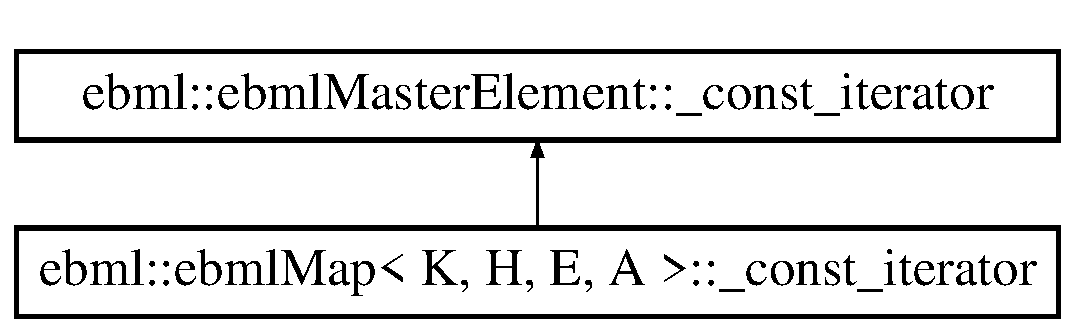
\includegraphics[height=2.000000cm]{classebml_1_1ebmlMap_1_1__const__iterator}
\end{center}
\end{figure}
\subsection*{Public Member Functions}
\begin{DoxyCompactItemize}
\item 
\mbox{\hyperlink{classebml_1_1ebmlMap_1_1__const__iterator_aaf09923a8b8d3f4edae2b54925966fa7}{\+\_\+const\+\_\+iterator}} ()
\item 
virtual \mbox{\hyperlink{classebml_1_1ebmlMap_1_1__const__iterator_a4f230319e3c3dfa23ed8418d05ec8cc6}{$\sim$\+\_\+const\+\_\+iterator}} ()
\item 
\mbox{\hyperlink{classebml_1_1ebmlMasterElement_1_1__const__iterator}{ebml\+Master\+Element\+::\+\_\+const\+\_\+iterator}} $\ast$ \mbox{\hyperlink{classebml_1_1ebmlMap_1_1__const__iterator_af2bd75417ff0115d8bb53670ff8deaf2}{copy}} () const
\item 
\mbox{\hyperlink{namespaceebml_a2deef4e8071531b32e3533f1bf978917}{c\+\_\+ebml\+Element\+\_\+sp}} \mbox{\hyperlink{classebml_1_1ebmlMap_1_1__const__iterator_a7385fe1f7e51cdf2c4c538e9cc474583}{operator$\ast$}} () const
\item 
\mbox{\hyperlink{classebml_1_1ebmlMasterElement_1_1__const__iterator}{ebml\+Master\+Element\+::\+\_\+const\+\_\+iterator}} \& \mbox{\hyperlink{classebml_1_1ebmlMap_1_1__const__iterator_a7a58190879091815afc606e295afd1cf}{operator++}} ()
\item 
\mbox{\hyperlink{classebml_1_1ebmlMasterElement_1_1__const__iterator}{ebml\+Master\+Element\+::\+\_\+const\+\_\+iterator}} \& \mbox{\hyperlink{classebml_1_1ebmlMap_1_1__const__iterator_a641afb65930e85882c6397d2f0930604}{operator=}} (const \mbox{\hyperlink{classebml_1_1ebmlMasterElement_1_1__const__iterator}{ebml\+Master\+Element\+::\+\_\+const\+\_\+iterator}} \&)
\item 
bool \mbox{\hyperlink{classebml_1_1ebmlMap_1_1__const__iterator_aa0b4af1c5b7d8bdb26def33c2a329371}{operator==}} (const \mbox{\hyperlink{classebml_1_1ebmlMasterElement_1_1__const__iterator}{ebml\+Master\+Element\+::\+\_\+const\+\_\+iterator}} \&) const
\item 
bool \mbox{\hyperlink{classebml_1_1ebmlMap_1_1__const__iterator_aa63b9e3fd20c1092792db91a25fb2b70}{operator!=}} (const \mbox{\hyperlink{classebml_1_1ebmlMasterElement_1_1__const__iterator}{ebml\+Master\+Element\+::\+\_\+const\+\_\+iterator}} \&) const
\end{DoxyCompactItemize}
\subsection*{Protected Member Functions}
\begin{DoxyCompactItemize}
\item 
\mbox{\hyperlink{classebml_1_1ebmlMap_1_1__const__iterator_a54489bbad9412f9adf099569a1f070d4}{\+\_\+const\+\_\+iterator}} (const \mbox{\hyperlink{namespaceebml_a2deef4e8071531b32e3533f1bf978917}{c\+\_\+ebml\+Element\+\_\+sp}} \&elem, const typename std\+::unordered\+\_\+map$<$ K, \mbox{\hyperlink{namespaceebml_adad533b7705a16bb360fe56380c5e7be}{ebml\+Element\+\_\+sp}}, H, E, A $>$\+::\mbox{\hyperlink{classebml_1_1ebmlMasterElement_1_1const__iterator}{const\+\_\+iterator}} \&iter)
\item 
\mbox{\hyperlink{classebml_1_1ebmlMap_1_1__const__iterator_a3e9d0048a1ec76406c6961f4d180bfbb}{\+\_\+const\+\_\+iterator}} (\mbox{\hyperlink{namespaceebml_a2deef4e8071531b32e3533f1bf978917}{c\+\_\+ebml\+Element\+\_\+sp}} \&\&elem, typename std\+::unordered\+\_\+map$<$ K, \mbox{\hyperlink{namespaceebml_adad533b7705a16bb360fe56380c5e7be}{ebml\+Element\+\_\+sp}}, H, E, A $>$\+::\mbox{\hyperlink{classebml_1_1ebmlMasterElement_1_1const__iterator}{const\+\_\+iterator}} \&\&iter)
\end{DoxyCompactItemize}
\subsection*{Friends}
\begin{DoxyCompactItemize}
\item 
class \mbox{\hyperlink{classebml_1_1ebmlMap_1_1__const__iterator_a691e480013452ea48661a61746fd1b5c}{ebml\+Map$<$ K, H, E, A $>$}}
\item 
class \mbox{\hyperlink{classebml_1_1ebmlMap_1_1__const__iterator_a734affd0f736e2e4e03ab2cf8a9f9b26}{ebml\+Master\+Element\+::const\+\_\+iterator}}
\end{DoxyCompactItemize}


\subsection{Constructor \& Destructor Documentation}
\mbox{\Hypertarget{classebml_1_1ebmlMap_1_1__const__iterator_a54489bbad9412f9adf099569a1f070d4}\label{classebml_1_1ebmlMap_1_1__const__iterator_a54489bbad9412f9adf099569a1f070d4}} 
\index{ebml\+::ebml\+Map\+::\+\_\+const\+\_\+iterator@{ebml\+::ebml\+Map\+::\+\_\+const\+\_\+iterator}!\+\_\+const\+\_\+iterator@{\+\_\+const\+\_\+iterator}}
\index{\+\_\+const\+\_\+iterator@{\+\_\+const\+\_\+iterator}!ebml\+::ebml\+Map\+::\+\_\+const\+\_\+iterator@{ebml\+::ebml\+Map\+::\+\_\+const\+\_\+iterator}}
\subsubsection{\texorpdfstring{\+\_\+const\+\_\+iterator()}{\_const\_iterator()}\hspace{0.1cm}{\footnotesize\ttfamily [1/3]}}
{\footnotesize\ttfamily template$<$typename K , typename H , typename E , typename A $>$ \\
\mbox{\hyperlink{classebml_1_1ebmlMap}{ebml\+::ebml\+Map}}$<$ K, H, E, A $>$\+::\+\_\+const\+\_\+iterator\+::\+\_\+const\+\_\+iterator (\begin{DoxyParamCaption}\item[{const \mbox{\hyperlink{namespaceebml_a2deef4e8071531b32e3533f1bf978917}{c\+\_\+ebml\+Element\+\_\+sp}} \&}]{elem,  }\item[{const typename std\+::unordered\+\_\+map$<$ K, \mbox{\hyperlink{namespaceebml_adad533b7705a16bb360fe56380c5e7be}{ebml\+Element\+\_\+sp}}, H, E, A $>$\+::\mbox{\hyperlink{classebml_1_1ebmlMasterElement_1_1const__iterator}{const\+\_\+iterator}} \&}]{iter }\end{DoxyParamCaption})\hspace{0.3cm}{\ttfamily [protected]}}

\mbox{\Hypertarget{classebml_1_1ebmlMap_1_1__const__iterator_a3e9d0048a1ec76406c6961f4d180bfbb}\label{classebml_1_1ebmlMap_1_1__const__iterator_a3e9d0048a1ec76406c6961f4d180bfbb}} 
\index{ebml\+::ebml\+Map\+::\+\_\+const\+\_\+iterator@{ebml\+::ebml\+Map\+::\+\_\+const\+\_\+iterator}!\+\_\+const\+\_\+iterator@{\+\_\+const\+\_\+iterator}}
\index{\+\_\+const\+\_\+iterator@{\+\_\+const\+\_\+iterator}!ebml\+::ebml\+Map\+::\+\_\+const\+\_\+iterator@{ebml\+::ebml\+Map\+::\+\_\+const\+\_\+iterator}}
\subsubsection{\texorpdfstring{\+\_\+const\+\_\+iterator()}{\_const\_iterator()}\hspace{0.1cm}{\footnotesize\ttfamily [2/3]}}
{\footnotesize\ttfamily template$<$typename K , typename H , typename E , typename A $>$ \\
\mbox{\hyperlink{classebml_1_1ebmlMap}{ebml\+::ebml\+Map}}$<$ K, H, E, A $>$\+::\+\_\+const\+\_\+iterator\+::\+\_\+const\+\_\+iterator (\begin{DoxyParamCaption}\item[{\mbox{\hyperlink{namespaceebml_a2deef4e8071531b32e3533f1bf978917}{c\+\_\+ebml\+Element\+\_\+sp}} \&\&}]{elem,  }\item[{typename std\+::unordered\+\_\+map$<$ K, \mbox{\hyperlink{namespaceebml_adad533b7705a16bb360fe56380c5e7be}{ebml\+Element\+\_\+sp}}, H, E, A $>$\+::\mbox{\hyperlink{classebml_1_1ebmlMasterElement_1_1const__iterator}{const\+\_\+iterator}} \&\&}]{iter }\end{DoxyParamCaption})\hspace{0.3cm}{\ttfamily [protected]}}

\mbox{\Hypertarget{classebml_1_1ebmlMap_1_1__const__iterator_aaf09923a8b8d3f4edae2b54925966fa7}\label{classebml_1_1ebmlMap_1_1__const__iterator_aaf09923a8b8d3f4edae2b54925966fa7}} 
\index{ebml\+::ebml\+Map\+::\+\_\+const\+\_\+iterator@{ebml\+::ebml\+Map\+::\+\_\+const\+\_\+iterator}!\+\_\+const\+\_\+iterator@{\+\_\+const\+\_\+iterator}}
\index{\+\_\+const\+\_\+iterator@{\+\_\+const\+\_\+iterator}!ebml\+::ebml\+Map\+::\+\_\+const\+\_\+iterator@{ebml\+::ebml\+Map\+::\+\_\+const\+\_\+iterator}}
\subsubsection{\texorpdfstring{\+\_\+const\+\_\+iterator()}{\_const\_iterator()}\hspace{0.1cm}{\footnotesize\ttfamily [3/3]}}
{\footnotesize\ttfamily template$<$typename K , typename H , typename E , typename A $>$ \\
\mbox{\hyperlink{classebml_1_1ebmlMap}{ebml\+::ebml\+Map}}$<$ K, H, E, A $>$\+::\+\_\+const\+\_\+iterator\+::\+\_\+const\+\_\+iterator (\begin{DoxyParamCaption}{ }\end{DoxyParamCaption})}

\mbox{\Hypertarget{classebml_1_1ebmlMap_1_1__const__iterator_a4f230319e3c3dfa23ed8418d05ec8cc6}\label{classebml_1_1ebmlMap_1_1__const__iterator_a4f230319e3c3dfa23ed8418d05ec8cc6}} 
\index{ebml\+::ebml\+Map\+::\+\_\+const\+\_\+iterator@{ebml\+::ebml\+Map\+::\+\_\+const\+\_\+iterator}!````~\+\_\+const\+\_\+iterator@{$\sim$\+\_\+const\+\_\+iterator}}
\index{````~\+\_\+const\+\_\+iterator@{$\sim$\+\_\+const\+\_\+iterator}!ebml\+::ebml\+Map\+::\+\_\+const\+\_\+iterator@{ebml\+::ebml\+Map\+::\+\_\+const\+\_\+iterator}}
\subsubsection{\texorpdfstring{$\sim$\+\_\+const\+\_\+iterator()}{~\_const\_iterator()}}
{\footnotesize\ttfamily template$<$typename K , typename H , typename E , typename A $>$ \\
virtual \mbox{\hyperlink{classebml_1_1ebmlMap}{ebml\+::ebml\+Map}}$<$ K, H, E, A $>$\+::\+\_\+const\+\_\+iterator\+::$\sim$\+\_\+const\+\_\+iterator (\begin{DoxyParamCaption}{ }\end{DoxyParamCaption})\hspace{0.3cm}{\ttfamily [virtual]}}



Reimplemented from \mbox{\hyperlink{classebml_1_1ebmlMasterElement_1_1__const__iterator_a6138f42b88ff06379d96a095a12ed136}{ebml\+::ebml\+Master\+Element\+::\+\_\+const\+\_\+iterator}}.



\subsection{Member Function Documentation}
\mbox{\Hypertarget{classebml_1_1ebmlMap_1_1__const__iterator_af2bd75417ff0115d8bb53670ff8deaf2}\label{classebml_1_1ebmlMap_1_1__const__iterator_af2bd75417ff0115d8bb53670ff8deaf2}} 
\index{ebml\+::ebml\+Map\+::\+\_\+const\+\_\+iterator@{ebml\+::ebml\+Map\+::\+\_\+const\+\_\+iterator}!copy@{copy}}
\index{copy@{copy}!ebml\+::ebml\+Map\+::\+\_\+const\+\_\+iterator@{ebml\+::ebml\+Map\+::\+\_\+const\+\_\+iterator}}
\subsubsection{\texorpdfstring{copy()}{copy()}}
{\footnotesize\ttfamily template$<$typename K , typename H , typename E , typename A $>$ \\
\mbox{\hyperlink{classebml_1_1ebmlMasterElement_1_1__const__iterator}{ebml\+Master\+Element\+::\+\_\+const\+\_\+iterator}}$\ast$ \mbox{\hyperlink{classebml_1_1ebmlMap}{ebml\+::ebml\+Map}}$<$ K, H, E, A $>$\+::\+\_\+const\+\_\+iterator\+::copy (\begin{DoxyParamCaption}{ }\end{DoxyParamCaption}) const\hspace{0.3cm}{\ttfamily [virtual]}}



Implements \mbox{\hyperlink{classebml_1_1ebmlMasterElement_1_1__const__iterator_a64a4853ad363358987eb6492579cd503}{ebml\+::ebml\+Master\+Element\+::\+\_\+const\+\_\+iterator}}.

\mbox{\Hypertarget{classebml_1_1ebmlMap_1_1__const__iterator_aa63b9e3fd20c1092792db91a25fb2b70}\label{classebml_1_1ebmlMap_1_1__const__iterator_aa63b9e3fd20c1092792db91a25fb2b70}} 
\index{ebml\+::ebml\+Map\+::\+\_\+const\+\_\+iterator@{ebml\+::ebml\+Map\+::\+\_\+const\+\_\+iterator}!operator"!=@{operator"!=}}
\index{operator"!=@{operator"!=}!ebml\+::ebml\+Map\+::\+\_\+const\+\_\+iterator@{ebml\+::ebml\+Map\+::\+\_\+const\+\_\+iterator}}
\subsubsection{\texorpdfstring{operator"!=()}{operator!=()}}
{\footnotesize\ttfamily template$<$typename K , typename H , typename E , typename A $>$ \\
bool \mbox{\hyperlink{classebml_1_1ebmlMap}{ebml\+::ebml\+Map}}$<$ K, H, E, A $>$\+::\+\_\+const\+\_\+iterator\+::operator!= (\begin{DoxyParamCaption}\item[{const \mbox{\hyperlink{classebml_1_1ebmlMasterElement_1_1__const__iterator}{ebml\+Master\+Element\+::\+\_\+const\+\_\+iterator}} \&}]{ }\end{DoxyParamCaption}) const\hspace{0.3cm}{\ttfamily [virtual]}}



Implements \mbox{\hyperlink{classebml_1_1ebmlMasterElement_1_1__const__iterator_ac62d190e9da49236835f8219ec307d22}{ebml\+::ebml\+Master\+Element\+::\+\_\+const\+\_\+iterator}}.

\mbox{\Hypertarget{classebml_1_1ebmlMap_1_1__const__iterator_a7385fe1f7e51cdf2c4c538e9cc474583}\label{classebml_1_1ebmlMap_1_1__const__iterator_a7385fe1f7e51cdf2c4c538e9cc474583}} 
\index{ebml\+::ebml\+Map\+::\+\_\+const\+\_\+iterator@{ebml\+::ebml\+Map\+::\+\_\+const\+\_\+iterator}!operator$\ast$@{operator$\ast$}}
\index{operator$\ast$@{operator$\ast$}!ebml\+::ebml\+Map\+::\+\_\+const\+\_\+iterator@{ebml\+::ebml\+Map\+::\+\_\+const\+\_\+iterator}}
\subsubsection{\texorpdfstring{operator$\ast$()}{operator*()}}
{\footnotesize\ttfamily template$<$typename K , typename H , typename E , typename A $>$ \\
\mbox{\hyperlink{namespaceebml_a2deef4e8071531b32e3533f1bf978917}{c\+\_\+ebml\+Element\+\_\+sp}} \mbox{\hyperlink{classebml_1_1ebmlMap}{ebml\+::ebml\+Map}}$<$ K, H, E, A $>$\+::\+\_\+const\+\_\+iterator\+::operator$\ast$ (\begin{DoxyParamCaption}{ }\end{DoxyParamCaption}) const\hspace{0.3cm}{\ttfamily [virtual]}}



Implements \mbox{\hyperlink{classebml_1_1ebmlMasterElement_1_1__const__iterator_aa3e5459826695a9043745fbbaea9cd47}{ebml\+::ebml\+Master\+Element\+::\+\_\+const\+\_\+iterator}}.

\mbox{\Hypertarget{classebml_1_1ebmlMap_1_1__const__iterator_a7a58190879091815afc606e295afd1cf}\label{classebml_1_1ebmlMap_1_1__const__iterator_a7a58190879091815afc606e295afd1cf}} 
\index{ebml\+::ebml\+Map\+::\+\_\+const\+\_\+iterator@{ebml\+::ebml\+Map\+::\+\_\+const\+\_\+iterator}!operator++@{operator++}}
\index{operator++@{operator++}!ebml\+::ebml\+Map\+::\+\_\+const\+\_\+iterator@{ebml\+::ebml\+Map\+::\+\_\+const\+\_\+iterator}}
\subsubsection{\texorpdfstring{operator++()}{operator++()}}
{\footnotesize\ttfamily template$<$typename K , typename H , typename E , typename A $>$ \\
\mbox{\hyperlink{classebml_1_1ebmlMasterElement_1_1__const__iterator}{ebml\+Master\+Element\+::\+\_\+const\+\_\+iterator}}\& \mbox{\hyperlink{classebml_1_1ebmlMap}{ebml\+::ebml\+Map}}$<$ K, H, E, A $>$\+::\+\_\+const\+\_\+iterator\+::operator++ (\begin{DoxyParamCaption}{ }\end{DoxyParamCaption})\hspace{0.3cm}{\ttfamily [virtual]}}



Implements \mbox{\hyperlink{classebml_1_1ebmlMasterElement_1_1__const__iterator_a439f540325443a3c3a3acdcd8df81553}{ebml\+::ebml\+Master\+Element\+::\+\_\+const\+\_\+iterator}}.

\mbox{\Hypertarget{classebml_1_1ebmlMap_1_1__const__iterator_a641afb65930e85882c6397d2f0930604}\label{classebml_1_1ebmlMap_1_1__const__iterator_a641afb65930e85882c6397d2f0930604}} 
\index{ebml\+::ebml\+Map\+::\+\_\+const\+\_\+iterator@{ebml\+::ebml\+Map\+::\+\_\+const\+\_\+iterator}!operator=@{operator=}}
\index{operator=@{operator=}!ebml\+::ebml\+Map\+::\+\_\+const\+\_\+iterator@{ebml\+::ebml\+Map\+::\+\_\+const\+\_\+iterator}}
\subsubsection{\texorpdfstring{operator=()}{operator=()}}
{\footnotesize\ttfamily template$<$typename K , typename H , typename E , typename A $>$ \\
\mbox{\hyperlink{classebml_1_1ebmlMasterElement_1_1__const__iterator}{ebml\+Master\+Element\+::\+\_\+const\+\_\+iterator}}\& \mbox{\hyperlink{classebml_1_1ebmlMap}{ebml\+::ebml\+Map}}$<$ K, H, E, A $>$\+::\+\_\+const\+\_\+iterator\+::operator= (\begin{DoxyParamCaption}\item[{const \mbox{\hyperlink{classebml_1_1ebmlMasterElement_1_1__const__iterator}{ebml\+Master\+Element\+::\+\_\+const\+\_\+iterator}} \&}]{ }\end{DoxyParamCaption})\hspace{0.3cm}{\ttfamily [virtual]}}



Implements \mbox{\hyperlink{classebml_1_1ebmlMasterElement_1_1__const__iterator_a102cf8b36c0d8184680ef15594bb59fb}{ebml\+::ebml\+Master\+Element\+::\+\_\+const\+\_\+iterator}}.

\mbox{\Hypertarget{classebml_1_1ebmlMap_1_1__const__iterator_aa0b4af1c5b7d8bdb26def33c2a329371}\label{classebml_1_1ebmlMap_1_1__const__iterator_aa0b4af1c5b7d8bdb26def33c2a329371}} 
\index{ebml\+::ebml\+Map\+::\+\_\+const\+\_\+iterator@{ebml\+::ebml\+Map\+::\+\_\+const\+\_\+iterator}!operator==@{operator==}}
\index{operator==@{operator==}!ebml\+::ebml\+Map\+::\+\_\+const\+\_\+iterator@{ebml\+::ebml\+Map\+::\+\_\+const\+\_\+iterator}}
\subsubsection{\texorpdfstring{operator==()}{operator==()}}
{\footnotesize\ttfamily template$<$typename K , typename H , typename E , typename A $>$ \\
bool \mbox{\hyperlink{classebml_1_1ebmlMap}{ebml\+::ebml\+Map}}$<$ K, H, E, A $>$\+::\+\_\+const\+\_\+iterator\+::operator== (\begin{DoxyParamCaption}\item[{const \mbox{\hyperlink{classebml_1_1ebmlMasterElement_1_1__const__iterator}{ebml\+Master\+Element\+::\+\_\+const\+\_\+iterator}} \&}]{ }\end{DoxyParamCaption}) const\hspace{0.3cm}{\ttfamily [virtual]}}



Implements \mbox{\hyperlink{classebml_1_1ebmlMasterElement_1_1__const__iterator_a936395ed4c0c189a92927bfdf1e28586}{ebml\+::ebml\+Master\+Element\+::\+\_\+const\+\_\+iterator}}.



\subsection{Friends And Related Function Documentation}
\mbox{\Hypertarget{classebml_1_1ebmlMap_1_1__const__iterator_a691e480013452ea48661a61746fd1b5c}\label{classebml_1_1ebmlMap_1_1__const__iterator_a691e480013452ea48661a61746fd1b5c}} 
\index{ebml\+::ebml\+Map\+::\+\_\+const\+\_\+iterator@{ebml\+::ebml\+Map\+::\+\_\+const\+\_\+iterator}!ebml\+Map$<$ K, H, E, A $>$@{ebml\+Map$<$ K, H, E, A $>$}}
\index{ebml\+Map$<$ K, H, E, A $>$@{ebml\+Map$<$ K, H, E, A $>$}!ebml\+::ebml\+Map\+::\+\_\+const\+\_\+iterator@{ebml\+::ebml\+Map\+::\+\_\+const\+\_\+iterator}}
\subsubsection{\texorpdfstring{ebml\+Map$<$ K, H, E, A $>$}{ebmlMap< K, H, E, A >}}
{\footnotesize\ttfamily template$<$typename K , typename H , typename E , typename A $>$ \\
friend class \mbox{\hyperlink{classebml_1_1ebmlMap}{ebml\+Map}}$<$ K, H, E, A $>$\hspace{0.3cm}{\ttfamily [friend]}}

\mbox{\Hypertarget{classebml_1_1ebmlMap_1_1__const__iterator_a734affd0f736e2e4e03ab2cf8a9f9b26}\label{classebml_1_1ebmlMap_1_1__const__iterator_a734affd0f736e2e4e03ab2cf8a9f9b26}} 
\index{ebml\+::ebml\+Map\+::\+\_\+const\+\_\+iterator@{ebml\+::ebml\+Map\+::\+\_\+const\+\_\+iterator}!ebml\+Master\+Element\+::const\+\_\+iterator@{ebml\+Master\+Element\+::const\+\_\+iterator}}
\index{ebml\+Master\+Element\+::const\+\_\+iterator@{ebml\+Master\+Element\+::const\+\_\+iterator}!ebml\+::ebml\+Map\+::\+\_\+const\+\_\+iterator@{ebml\+::ebml\+Map\+::\+\_\+const\+\_\+iterator}}
\subsubsection{\texorpdfstring{ebml\+Master\+Element\+::const\+\_\+iterator}{ebmlMasterElement::const\_iterator}}
{\footnotesize\ttfamily template$<$typename K , typename H , typename E , typename A $>$ \\
friend class \mbox{\hyperlink{classebml_1_1ebmlMasterElement_1_1const__iterator}{ebml\+Master\+Element\+::const\+\_\+iterator}}\hspace{0.3cm}{\ttfamily [friend]}}



The documentation for this class was generated from the following file\+:\begin{DoxyCompactItemize}
\item 
include/libebml\+\_\+ng/masterelement/\mbox{\hyperlink{map_8h}{map.\+h}}\end{DoxyCompactItemize}

\hypertarget{classebml_1_1ebmlMultiSlot_1_1__const__iterator}{}\section{ebml\+:\+:ebml\+Multi\+Slot\+:\+:\+\_\+const\+\_\+iterator Class Reference}
\label{classebml_1_1ebmlMultiSlot_1_1__const__iterator}\index{ebml\+::ebml\+Multi\+Slot\+::\+\_\+const\+\_\+iterator@{ebml\+::ebml\+Multi\+Slot\+::\+\_\+const\+\_\+iterator}}


{\ttfamily \#include $<$multislot.\+h$>$}

Inheritance diagram for ebml\+:\+:ebml\+Multi\+Slot\+:\+:\+\_\+const\+\_\+iterator\+:\begin{figure}[H]
\begin{center}
\leavevmode
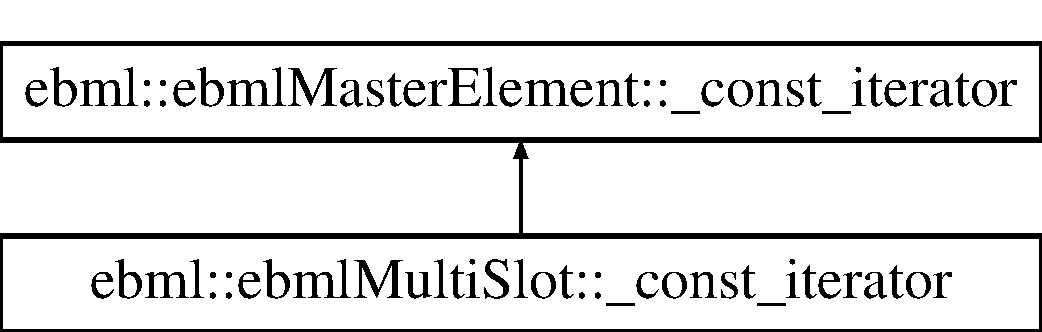
\includegraphics[height=2.000000cm]{classebml_1_1ebmlMultiSlot_1_1__const__iterator}
\end{center}
\end{figure}
\subsection*{Public Member Functions}
\begin{DoxyCompactItemize}
\item 
\mbox{\hyperlink{classebml_1_1ebmlMultiSlot_1_1__const__iterator_ab8933d3fbdbf45d65ec3731f667c1a79}{\+\_\+const\+\_\+iterator}} ()
\item 
virtual \mbox{\hyperlink{classebml_1_1ebmlMultiSlot_1_1__const__iterator_af518a921ebb2e2734b4d045d7d8be0f1}{$\sim$\+\_\+const\+\_\+iterator}} ()
\item 
\mbox{\hyperlink{classebml_1_1ebmlMasterElement_1_1__const__iterator}{ebml\+Master\+Element\+::\+\_\+const\+\_\+iterator}} $\ast$ \mbox{\hyperlink{classebml_1_1ebmlMultiSlot_1_1__const__iterator_a412c3cc02df5d62c4a05be31aca752e5}{copy}} () const
\item 
\mbox{\hyperlink{namespaceebml_a2deef4e8071531b32e3533f1bf978917}{c\+\_\+ebml\+Element\+\_\+sp}} \mbox{\hyperlink{classebml_1_1ebmlMultiSlot_1_1__const__iterator_ad4dfa7a3f08d535fe83c93c762009483}{operator$\ast$}} () const
\item 
\mbox{\hyperlink{classebml_1_1ebmlMasterElement_1_1__const__iterator}{ebml\+Master\+Element\+::\+\_\+const\+\_\+iterator}} \& \mbox{\hyperlink{classebml_1_1ebmlMultiSlot_1_1__const__iterator_a4d9425007a96cb4803ef3cff5bf88e00}{operator++}} ()
\item 
\mbox{\hyperlink{classebml_1_1ebmlMasterElement_1_1__const__iterator}{ebml\+Master\+Element\+::\+\_\+const\+\_\+iterator}} \& \mbox{\hyperlink{classebml_1_1ebmlMultiSlot_1_1__const__iterator_a6e2de45285786f1045fef8be51974b0b}{operator=}} (const \mbox{\hyperlink{classebml_1_1ebmlMasterElement_1_1__const__iterator}{ebml\+Master\+Element\+::\+\_\+const\+\_\+iterator}} \&)
\item 
bool \mbox{\hyperlink{classebml_1_1ebmlMultiSlot_1_1__const__iterator_a874e71d4f6d86e1213c8381ec20f3069}{operator==}} (const \mbox{\hyperlink{classebml_1_1ebmlMasterElement_1_1__const__iterator}{ebml\+Master\+Element\+::\+\_\+const\+\_\+iterator}} \&) const
\item 
bool \mbox{\hyperlink{classebml_1_1ebmlMultiSlot_1_1__const__iterator_a9a1c8df8a22d52ecb55de9f151f383e0}{operator!=}} (const \mbox{\hyperlink{classebml_1_1ebmlMasterElement_1_1__const__iterator}{ebml\+Master\+Element\+::\+\_\+const\+\_\+iterator}} \&) const
\end{DoxyCompactItemize}
\subsection*{Protected Member Functions}
\begin{DoxyCompactItemize}
\item 
\mbox{\hyperlink{classebml_1_1ebmlMultiSlot_1_1__const__iterator_a5b4e23f10ca68b3ada0101d6a085f48d}{\+\_\+const\+\_\+iterator}} (const \mbox{\hyperlink{namespaceebml_a2deef4e8071531b32e3533f1bf978917}{c\+\_\+ebml\+Element\+\_\+sp}} \&elem, const std\+::vector$<$ \+\_\+slot\+\_\+t $>$\+::\mbox{\hyperlink{classebml_1_1ebmlMasterElement_1_1const__iterator}{const\+\_\+iterator}} \&slotiter, const std\+::vector$<$ \+\_\+slot\+\_\+t $>$\+::\mbox{\hyperlink{classebml_1_1ebmlMasterElement_1_1const__iterator}{const\+\_\+iterator}} \&slotiterend, const \mbox{\hyperlink{classebml_1_1const__slot__t_1_1iterator}{const\+\_\+slot\+\_\+t\+::iterator}} \&iter, const \mbox{\hyperlink{classebml_1_1const__slot__t_1_1iterator}{const\+\_\+slot\+\_\+t\+::iterator}} \&iterend)
\item 
\mbox{\hyperlink{classebml_1_1ebmlMultiSlot_1_1__const__iterator_a681e9596c1ae982f3c482548cb16333d}{\+\_\+const\+\_\+iterator}} (\mbox{\hyperlink{namespaceebml_a2deef4e8071531b32e3533f1bf978917}{c\+\_\+ebml\+Element\+\_\+sp}} \&\&elem, std\+::vector$<$ \+\_\+slot\+\_\+t $>$\+::\mbox{\hyperlink{classebml_1_1ebmlMasterElement_1_1const__iterator}{const\+\_\+iterator}} \&\&slotiter, std\+::vector$<$ \+\_\+slot\+\_\+t $>$\+::\mbox{\hyperlink{classebml_1_1ebmlMasterElement_1_1const__iterator}{const\+\_\+iterator}} \&\&slotiterend, \mbox{\hyperlink{classebml_1_1const__slot__t_1_1iterator}{const\+\_\+slot\+\_\+t\+::iterator}} \&\&iter, \mbox{\hyperlink{classebml_1_1const__slot__t_1_1iterator}{const\+\_\+slot\+\_\+t\+::iterator}} \&\&iterend)
\end{DoxyCompactItemize}
\subsection*{Friends}
\begin{DoxyCompactItemize}
\item 
class \mbox{\hyperlink{classebml_1_1ebmlMultiSlot_1_1__const__iterator_ab14eb6c5a125d7276a7b4b5b6573428b}{ebml\+Multi\+Slot}}
\item 
class \mbox{\hyperlink{classebml_1_1ebmlMultiSlot_1_1__const__iterator_a734affd0f736e2e4e03ab2cf8a9f9b26}{ebml\+Master\+Element\+::const\+\_\+iterator}}
\end{DoxyCompactItemize}


\subsection{Constructor \& Destructor Documentation}
\mbox{\Hypertarget{classebml_1_1ebmlMultiSlot_1_1__const__iterator_a5b4e23f10ca68b3ada0101d6a085f48d}\label{classebml_1_1ebmlMultiSlot_1_1__const__iterator_a5b4e23f10ca68b3ada0101d6a085f48d}} 
\index{ebml\+::ebml\+Multi\+Slot\+::\+\_\+const\+\_\+iterator@{ebml\+::ebml\+Multi\+Slot\+::\+\_\+const\+\_\+iterator}!\+\_\+const\+\_\+iterator@{\+\_\+const\+\_\+iterator}}
\index{\+\_\+const\+\_\+iterator@{\+\_\+const\+\_\+iterator}!ebml\+::ebml\+Multi\+Slot\+::\+\_\+const\+\_\+iterator@{ebml\+::ebml\+Multi\+Slot\+::\+\_\+const\+\_\+iterator}}
\subsubsection{\texorpdfstring{\+\_\+const\+\_\+iterator()}{\_const\_iterator()}\hspace{0.1cm}{\footnotesize\ttfamily [1/3]}}
{\footnotesize\ttfamily ebml\+::ebml\+Multi\+Slot\+::\+\_\+const\+\_\+iterator\+::\+\_\+const\+\_\+iterator (\begin{DoxyParamCaption}\item[{const \mbox{\hyperlink{namespaceebml_a2deef4e8071531b32e3533f1bf978917}{c\+\_\+ebml\+Element\+\_\+sp}} \&}]{elem,  }\item[{const std\+::vector$<$ \+\_\+slot\+\_\+t $>$\+::\mbox{\hyperlink{classebml_1_1ebmlMasterElement_1_1const__iterator}{const\+\_\+iterator}} \&}]{slotiter,  }\item[{const std\+::vector$<$ \+\_\+slot\+\_\+t $>$\+::\mbox{\hyperlink{classebml_1_1ebmlMasterElement_1_1const__iterator}{const\+\_\+iterator}} \&}]{slotiterend,  }\item[{const \mbox{\hyperlink{classebml_1_1const__slot__t_1_1iterator}{const\+\_\+slot\+\_\+t\+::iterator}} \&}]{iter,  }\item[{const \mbox{\hyperlink{classebml_1_1const__slot__t_1_1iterator}{const\+\_\+slot\+\_\+t\+::iterator}} \&}]{iterend }\end{DoxyParamCaption})\hspace{0.3cm}{\ttfamily [protected]}}

\mbox{\Hypertarget{classebml_1_1ebmlMultiSlot_1_1__const__iterator_a681e9596c1ae982f3c482548cb16333d}\label{classebml_1_1ebmlMultiSlot_1_1__const__iterator_a681e9596c1ae982f3c482548cb16333d}} 
\index{ebml\+::ebml\+Multi\+Slot\+::\+\_\+const\+\_\+iterator@{ebml\+::ebml\+Multi\+Slot\+::\+\_\+const\+\_\+iterator}!\+\_\+const\+\_\+iterator@{\+\_\+const\+\_\+iterator}}
\index{\+\_\+const\+\_\+iterator@{\+\_\+const\+\_\+iterator}!ebml\+::ebml\+Multi\+Slot\+::\+\_\+const\+\_\+iterator@{ebml\+::ebml\+Multi\+Slot\+::\+\_\+const\+\_\+iterator}}
\subsubsection{\texorpdfstring{\+\_\+const\+\_\+iterator()}{\_const\_iterator()}\hspace{0.1cm}{\footnotesize\ttfamily [2/3]}}
{\footnotesize\ttfamily ebml\+::ebml\+Multi\+Slot\+::\+\_\+const\+\_\+iterator\+::\+\_\+const\+\_\+iterator (\begin{DoxyParamCaption}\item[{\mbox{\hyperlink{namespaceebml_a2deef4e8071531b32e3533f1bf978917}{c\+\_\+ebml\+Element\+\_\+sp}} \&\&}]{elem,  }\item[{std\+::vector$<$ \+\_\+slot\+\_\+t $>$\+::\mbox{\hyperlink{classebml_1_1ebmlMasterElement_1_1const__iterator}{const\+\_\+iterator}} \&\&}]{slotiter,  }\item[{std\+::vector$<$ \+\_\+slot\+\_\+t $>$\+::\mbox{\hyperlink{classebml_1_1ebmlMasterElement_1_1const__iterator}{const\+\_\+iterator}} \&\&}]{slotiterend,  }\item[{\mbox{\hyperlink{classebml_1_1const__slot__t_1_1iterator}{const\+\_\+slot\+\_\+t\+::iterator}} \&\&}]{iter,  }\item[{\mbox{\hyperlink{classebml_1_1const__slot__t_1_1iterator}{const\+\_\+slot\+\_\+t\+::iterator}} \&\&}]{iterend }\end{DoxyParamCaption})\hspace{0.3cm}{\ttfamily [protected]}}

\mbox{\Hypertarget{classebml_1_1ebmlMultiSlot_1_1__const__iterator_ab8933d3fbdbf45d65ec3731f667c1a79}\label{classebml_1_1ebmlMultiSlot_1_1__const__iterator_ab8933d3fbdbf45d65ec3731f667c1a79}} 
\index{ebml\+::ebml\+Multi\+Slot\+::\+\_\+const\+\_\+iterator@{ebml\+::ebml\+Multi\+Slot\+::\+\_\+const\+\_\+iterator}!\+\_\+const\+\_\+iterator@{\+\_\+const\+\_\+iterator}}
\index{\+\_\+const\+\_\+iterator@{\+\_\+const\+\_\+iterator}!ebml\+::ebml\+Multi\+Slot\+::\+\_\+const\+\_\+iterator@{ebml\+::ebml\+Multi\+Slot\+::\+\_\+const\+\_\+iterator}}
\subsubsection{\texorpdfstring{\+\_\+const\+\_\+iterator()}{\_const\_iterator()}\hspace{0.1cm}{\footnotesize\ttfamily [3/3]}}
{\footnotesize\ttfamily ebml\+::ebml\+Multi\+Slot\+::\+\_\+const\+\_\+iterator\+::\+\_\+const\+\_\+iterator (\begin{DoxyParamCaption}{ }\end{DoxyParamCaption})}

\mbox{\Hypertarget{classebml_1_1ebmlMultiSlot_1_1__const__iterator_af518a921ebb2e2734b4d045d7d8be0f1}\label{classebml_1_1ebmlMultiSlot_1_1__const__iterator_af518a921ebb2e2734b4d045d7d8be0f1}} 
\index{ebml\+::ebml\+Multi\+Slot\+::\+\_\+const\+\_\+iterator@{ebml\+::ebml\+Multi\+Slot\+::\+\_\+const\+\_\+iterator}!````~\+\_\+const\+\_\+iterator@{$\sim$\+\_\+const\+\_\+iterator}}
\index{````~\+\_\+const\+\_\+iterator@{$\sim$\+\_\+const\+\_\+iterator}!ebml\+::ebml\+Multi\+Slot\+::\+\_\+const\+\_\+iterator@{ebml\+::ebml\+Multi\+Slot\+::\+\_\+const\+\_\+iterator}}
\subsubsection{\texorpdfstring{$\sim$\+\_\+const\+\_\+iterator()}{~\_const\_iterator()}}
{\footnotesize\ttfamily virtual ebml\+::ebml\+Multi\+Slot\+::\+\_\+const\+\_\+iterator\+::$\sim$\+\_\+const\+\_\+iterator (\begin{DoxyParamCaption}{ }\end{DoxyParamCaption})\hspace{0.3cm}{\ttfamily [virtual]}}



Reimplemented from \mbox{\hyperlink{classebml_1_1ebmlMasterElement_1_1__const__iterator_a6138f42b88ff06379d96a095a12ed136}{ebml\+::ebml\+Master\+Element\+::\+\_\+const\+\_\+iterator}}.



\subsection{Member Function Documentation}
\mbox{\Hypertarget{classebml_1_1ebmlMultiSlot_1_1__const__iterator_a412c3cc02df5d62c4a05be31aca752e5}\label{classebml_1_1ebmlMultiSlot_1_1__const__iterator_a412c3cc02df5d62c4a05be31aca752e5}} 
\index{ebml\+::ebml\+Multi\+Slot\+::\+\_\+const\+\_\+iterator@{ebml\+::ebml\+Multi\+Slot\+::\+\_\+const\+\_\+iterator}!copy@{copy}}
\index{copy@{copy}!ebml\+::ebml\+Multi\+Slot\+::\+\_\+const\+\_\+iterator@{ebml\+::ebml\+Multi\+Slot\+::\+\_\+const\+\_\+iterator}}
\subsubsection{\texorpdfstring{copy()}{copy()}}
{\footnotesize\ttfamily \mbox{\hyperlink{classebml_1_1ebmlMasterElement_1_1__const__iterator}{ebml\+Master\+Element\+::\+\_\+const\+\_\+iterator}}$\ast$ ebml\+::ebml\+Multi\+Slot\+::\+\_\+const\+\_\+iterator\+::copy (\begin{DoxyParamCaption}{ }\end{DoxyParamCaption}) const\hspace{0.3cm}{\ttfamily [virtual]}}



Implements \mbox{\hyperlink{classebml_1_1ebmlMasterElement_1_1__const__iterator_a64a4853ad363358987eb6492579cd503}{ebml\+::ebml\+Master\+Element\+::\+\_\+const\+\_\+iterator}}.

\mbox{\Hypertarget{classebml_1_1ebmlMultiSlot_1_1__const__iterator_a9a1c8df8a22d52ecb55de9f151f383e0}\label{classebml_1_1ebmlMultiSlot_1_1__const__iterator_a9a1c8df8a22d52ecb55de9f151f383e0}} 
\index{ebml\+::ebml\+Multi\+Slot\+::\+\_\+const\+\_\+iterator@{ebml\+::ebml\+Multi\+Slot\+::\+\_\+const\+\_\+iterator}!operator"!=@{operator"!=}}
\index{operator"!=@{operator"!=}!ebml\+::ebml\+Multi\+Slot\+::\+\_\+const\+\_\+iterator@{ebml\+::ebml\+Multi\+Slot\+::\+\_\+const\+\_\+iterator}}
\subsubsection{\texorpdfstring{operator"!=()}{operator!=()}}
{\footnotesize\ttfamily bool ebml\+::ebml\+Multi\+Slot\+::\+\_\+const\+\_\+iterator\+::operator!= (\begin{DoxyParamCaption}\item[{const \mbox{\hyperlink{classebml_1_1ebmlMasterElement_1_1__const__iterator}{ebml\+Master\+Element\+::\+\_\+const\+\_\+iterator}} \&}]{ }\end{DoxyParamCaption}) const\hspace{0.3cm}{\ttfamily [virtual]}}



Implements \mbox{\hyperlink{classebml_1_1ebmlMasterElement_1_1__const__iterator_ac62d190e9da49236835f8219ec307d22}{ebml\+::ebml\+Master\+Element\+::\+\_\+const\+\_\+iterator}}.

\mbox{\Hypertarget{classebml_1_1ebmlMultiSlot_1_1__const__iterator_ad4dfa7a3f08d535fe83c93c762009483}\label{classebml_1_1ebmlMultiSlot_1_1__const__iterator_ad4dfa7a3f08d535fe83c93c762009483}} 
\index{ebml\+::ebml\+Multi\+Slot\+::\+\_\+const\+\_\+iterator@{ebml\+::ebml\+Multi\+Slot\+::\+\_\+const\+\_\+iterator}!operator$\ast$@{operator$\ast$}}
\index{operator$\ast$@{operator$\ast$}!ebml\+::ebml\+Multi\+Slot\+::\+\_\+const\+\_\+iterator@{ebml\+::ebml\+Multi\+Slot\+::\+\_\+const\+\_\+iterator}}
\subsubsection{\texorpdfstring{operator$\ast$()}{operator*()}}
{\footnotesize\ttfamily \mbox{\hyperlink{namespaceebml_a2deef4e8071531b32e3533f1bf978917}{c\+\_\+ebml\+Element\+\_\+sp}} ebml\+::ebml\+Multi\+Slot\+::\+\_\+const\+\_\+iterator\+::operator$\ast$ (\begin{DoxyParamCaption}{ }\end{DoxyParamCaption}) const\hspace{0.3cm}{\ttfamily [virtual]}}



Implements \mbox{\hyperlink{classebml_1_1ebmlMasterElement_1_1__const__iterator_aa3e5459826695a9043745fbbaea9cd47}{ebml\+::ebml\+Master\+Element\+::\+\_\+const\+\_\+iterator}}.

\mbox{\Hypertarget{classebml_1_1ebmlMultiSlot_1_1__const__iterator_a4d9425007a96cb4803ef3cff5bf88e00}\label{classebml_1_1ebmlMultiSlot_1_1__const__iterator_a4d9425007a96cb4803ef3cff5bf88e00}} 
\index{ebml\+::ebml\+Multi\+Slot\+::\+\_\+const\+\_\+iterator@{ebml\+::ebml\+Multi\+Slot\+::\+\_\+const\+\_\+iterator}!operator++@{operator++}}
\index{operator++@{operator++}!ebml\+::ebml\+Multi\+Slot\+::\+\_\+const\+\_\+iterator@{ebml\+::ebml\+Multi\+Slot\+::\+\_\+const\+\_\+iterator}}
\subsubsection{\texorpdfstring{operator++()}{operator++()}}
{\footnotesize\ttfamily \mbox{\hyperlink{classebml_1_1ebmlMasterElement_1_1__const__iterator}{ebml\+Master\+Element\+::\+\_\+const\+\_\+iterator}}\& ebml\+::ebml\+Multi\+Slot\+::\+\_\+const\+\_\+iterator\+::operator++ (\begin{DoxyParamCaption}{ }\end{DoxyParamCaption})\hspace{0.3cm}{\ttfamily [virtual]}}



Implements \mbox{\hyperlink{classebml_1_1ebmlMasterElement_1_1__const__iterator_a439f540325443a3c3a3acdcd8df81553}{ebml\+::ebml\+Master\+Element\+::\+\_\+const\+\_\+iterator}}.

\mbox{\Hypertarget{classebml_1_1ebmlMultiSlot_1_1__const__iterator_a6e2de45285786f1045fef8be51974b0b}\label{classebml_1_1ebmlMultiSlot_1_1__const__iterator_a6e2de45285786f1045fef8be51974b0b}} 
\index{ebml\+::ebml\+Multi\+Slot\+::\+\_\+const\+\_\+iterator@{ebml\+::ebml\+Multi\+Slot\+::\+\_\+const\+\_\+iterator}!operator=@{operator=}}
\index{operator=@{operator=}!ebml\+::ebml\+Multi\+Slot\+::\+\_\+const\+\_\+iterator@{ebml\+::ebml\+Multi\+Slot\+::\+\_\+const\+\_\+iterator}}
\subsubsection{\texorpdfstring{operator=()}{operator=()}}
{\footnotesize\ttfamily \mbox{\hyperlink{classebml_1_1ebmlMasterElement_1_1__const__iterator}{ebml\+Master\+Element\+::\+\_\+const\+\_\+iterator}}\& ebml\+::ebml\+Multi\+Slot\+::\+\_\+const\+\_\+iterator\+::operator= (\begin{DoxyParamCaption}\item[{const \mbox{\hyperlink{classebml_1_1ebmlMasterElement_1_1__const__iterator}{ebml\+Master\+Element\+::\+\_\+const\+\_\+iterator}} \&}]{ }\end{DoxyParamCaption})\hspace{0.3cm}{\ttfamily [virtual]}}



Implements \mbox{\hyperlink{classebml_1_1ebmlMasterElement_1_1__const__iterator_a102cf8b36c0d8184680ef15594bb59fb}{ebml\+::ebml\+Master\+Element\+::\+\_\+const\+\_\+iterator}}.

\mbox{\Hypertarget{classebml_1_1ebmlMultiSlot_1_1__const__iterator_a874e71d4f6d86e1213c8381ec20f3069}\label{classebml_1_1ebmlMultiSlot_1_1__const__iterator_a874e71d4f6d86e1213c8381ec20f3069}} 
\index{ebml\+::ebml\+Multi\+Slot\+::\+\_\+const\+\_\+iterator@{ebml\+::ebml\+Multi\+Slot\+::\+\_\+const\+\_\+iterator}!operator==@{operator==}}
\index{operator==@{operator==}!ebml\+::ebml\+Multi\+Slot\+::\+\_\+const\+\_\+iterator@{ebml\+::ebml\+Multi\+Slot\+::\+\_\+const\+\_\+iterator}}
\subsubsection{\texorpdfstring{operator==()}{operator==()}}
{\footnotesize\ttfamily bool ebml\+::ebml\+Multi\+Slot\+::\+\_\+const\+\_\+iterator\+::operator== (\begin{DoxyParamCaption}\item[{const \mbox{\hyperlink{classebml_1_1ebmlMasterElement_1_1__const__iterator}{ebml\+Master\+Element\+::\+\_\+const\+\_\+iterator}} \&}]{ }\end{DoxyParamCaption}) const\hspace{0.3cm}{\ttfamily [virtual]}}



Implements \mbox{\hyperlink{classebml_1_1ebmlMasterElement_1_1__const__iterator_a936395ed4c0c189a92927bfdf1e28586}{ebml\+::ebml\+Master\+Element\+::\+\_\+const\+\_\+iterator}}.



\subsection{Friends And Related Function Documentation}
\mbox{\Hypertarget{classebml_1_1ebmlMultiSlot_1_1__const__iterator_a734affd0f736e2e4e03ab2cf8a9f9b26}\label{classebml_1_1ebmlMultiSlot_1_1__const__iterator_a734affd0f736e2e4e03ab2cf8a9f9b26}} 
\index{ebml\+::ebml\+Multi\+Slot\+::\+\_\+const\+\_\+iterator@{ebml\+::ebml\+Multi\+Slot\+::\+\_\+const\+\_\+iterator}!ebml\+Master\+Element\+::const\+\_\+iterator@{ebml\+Master\+Element\+::const\+\_\+iterator}}
\index{ebml\+Master\+Element\+::const\+\_\+iterator@{ebml\+Master\+Element\+::const\+\_\+iterator}!ebml\+::ebml\+Multi\+Slot\+::\+\_\+const\+\_\+iterator@{ebml\+::ebml\+Multi\+Slot\+::\+\_\+const\+\_\+iterator}}
\subsubsection{\texorpdfstring{ebml\+Master\+Element\+::const\+\_\+iterator}{ebmlMasterElement::const\_iterator}}
{\footnotesize\ttfamily friend class \mbox{\hyperlink{classebml_1_1ebmlMasterElement_1_1const__iterator}{ebml\+Master\+Element\+::const\+\_\+iterator}}\hspace{0.3cm}{\ttfamily [friend]}}

\mbox{\Hypertarget{classebml_1_1ebmlMultiSlot_1_1__const__iterator_ab14eb6c5a125d7276a7b4b5b6573428b}\label{classebml_1_1ebmlMultiSlot_1_1__const__iterator_ab14eb6c5a125d7276a7b4b5b6573428b}} 
\index{ebml\+::ebml\+Multi\+Slot\+::\+\_\+const\+\_\+iterator@{ebml\+::ebml\+Multi\+Slot\+::\+\_\+const\+\_\+iterator}!ebml\+Multi\+Slot@{ebml\+Multi\+Slot}}
\index{ebml\+Multi\+Slot@{ebml\+Multi\+Slot}!ebml\+::ebml\+Multi\+Slot\+::\+\_\+const\+\_\+iterator@{ebml\+::ebml\+Multi\+Slot\+::\+\_\+const\+\_\+iterator}}
\subsubsection{\texorpdfstring{ebml\+Multi\+Slot}{ebmlMultiSlot}}
{\footnotesize\ttfamily friend class \mbox{\hyperlink{classebml_1_1ebmlMultiSlot}{ebml\+Multi\+Slot}}\hspace{0.3cm}{\ttfamily [friend]}}



The documentation for this class was generated from the following file\+:\begin{DoxyCompactItemize}
\item 
include/libebml\+\_\+ng/masterelement/\mbox{\hyperlink{multislot_8h}{multislot.\+h}}\end{DoxyCompactItemize}

\hypertarget{classebml_1_1ebmlMasterElement_1_1__iterator}{}\section{ebml\+:\+:ebml\+Master\+Element\+:\+:\+\_\+iterator Class Reference}
\label{classebml_1_1ebmlMasterElement_1_1__iterator}\index{ebml\+::ebml\+Master\+Element\+::\+\_\+iterator@{ebml\+::ebml\+Master\+Element\+::\+\_\+iterator}}


{\ttfamily \#include $<$base.\+h$>$}

Inheritance diagram for ebml\+:\+:ebml\+Master\+Element\+:\+:\+\_\+iterator\+:\begin{figure}[H]
\begin{center}
\leavevmode
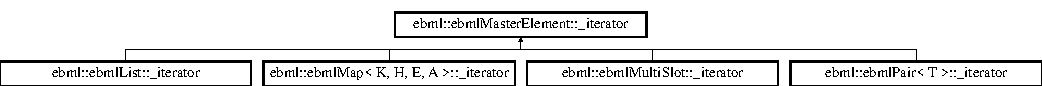
\includegraphics[height=1.161826cm]{classebml_1_1ebmlMasterElement_1_1__iterator}
\end{center}
\end{figure}
\subsection*{Public Member Functions}
\begin{DoxyCompactItemize}
\item 
virtual \mbox{\hyperlink{classebml_1_1ebmlMasterElement_1_1__iterator}{\+\_\+iterator}} $\ast$ \mbox{\hyperlink{classebml_1_1ebmlMasterElement_1_1__iterator_af9f522b6d6f34acb410add9579a35c13}{copy}} () const =0
\item 
virtual const \mbox{\hyperlink{namespaceebml_adad533b7705a16bb360fe56380c5e7be}{ebml\+Element\+\_\+sp}} \& \mbox{\hyperlink{classebml_1_1ebmlMasterElement_1_1__iterator_a3275ab5cdba37d79dd323879598f4f5d}{operator$\ast$}} () const =0
\item 
virtual \mbox{\hyperlink{classebml_1_1ebmlMasterElement_1_1__iterator}{\+\_\+iterator}} \& \mbox{\hyperlink{classebml_1_1ebmlMasterElement_1_1__iterator_ab77210fd0e481e1bb5b8563f7bd8142b}{operator++}} ()=0
\item 
virtual \mbox{\hyperlink{classebml_1_1ebmlMasterElement_1_1__iterator}{\+\_\+iterator}} \& \mbox{\hyperlink{classebml_1_1ebmlMasterElement_1_1__iterator_a849c5027957fa1a022de0417aea1ad9e}{operator=}} (const \mbox{\hyperlink{classebml_1_1ebmlMasterElement_1_1__iterator}{\+\_\+iterator}} \&)=0
\item 
virtual bool \mbox{\hyperlink{classebml_1_1ebmlMasterElement_1_1__iterator_ab0b53665f686e2ae379b275110ea3c95}{operator==}} (const \mbox{\hyperlink{classebml_1_1ebmlMasterElement_1_1__iterator}{\+\_\+iterator}} \&) const =0
\item 
virtual bool \mbox{\hyperlink{classebml_1_1ebmlMasterElement_1_1__iterator_aef9e45972d70a546942f9de73af40dc2}{operator!=}} (const \mbox{\hyperlink{classebml_1_1ebmlMasterElement_1_1__iterator}{\+\_\+iterator}} \&) const =0
\item 
virtual \mbox{\hyperlink{classebml_1_1ebmlMasterElement_1_1__iterator_a499f5fe9a5dddf51dd0ca181fc98f561}{$\sim$\+\_\+iterator}} ()
\end{DoxyCompactItemize}
\subsection*{Friends}
\begin{DoxyCompactItemize}
\item 
class \mbox{\hyperlink{classebml_1_1ebmlMasterElement_1_1__iterator_ad88e86cba72e9332a4693c1c6009b281}{ebml\+Master\+Element}}
\item 
class \mbox{\hyperlink{classebml_1_1ebmlMasterElement_1_1__iterator_a7f678a46134f738b99dfff4aafa7fc5f}{ebml\+Master\+Element\+::iterator}}
\end{DoxyCompactItemize}


\subsection{Constructor \& Destructor Documentation}
\mbox{\Hypertarget{classebml_1_1ebmlMasterElement_1_1__iterator_a499f5fe9a5dddf51dd0ca181fc98f561}\label{classebml_1_1ebmlMasterElement_1_1__iterator_a499f5fe9a5dddf51dd0ca181fc98f561}} 
\index{ebml\+::ebml\+Master\+Element\+::\+\_\+iterator@{ebml\+::ebml\+Master\+Element\+::\+\_\+iterator}!````~\+\_\+iterator@{$\sim$\+\_\+iterator}}
\index{````~\+\_\+iterator@{$\sim$\+\_\+iterator}!ebml\+::ebml\+Master\+Element\+::\+\_\+iterator@{ebml\+::ebml\+Master\+Element\+::\+\_\+iterator}}
\subsubsection{\texorpdfstring{$\sim$\+\_\+iterator()}{~\_iterator()}}
{\footnotesize\ttfamily virtual ebml\+::ebml\+Master\+Element\+::\+\_\+iterator\+::$\sim$\+\_\+iterator (\begin{DoxyParamCaption}{ }\end{DoxyParamCaption})\hspace{0.3cm}{\ttfamily [inline]}, {\ttfamily [virtual]}}



Reimplemented in \mbox{\hyperlink{classebml_1_1ebmlMultiSlot_1_1__iterator_a1d4b6ffee0d593ee22ac312d61d99d16}{ebml\+::ebml\+Multi\+Slot\+::\+\_\+iterator}}, \mbox{\hyperlink{classebml_1_1ebmlMap_1_1__iterator_a276c17f3a552f25f09735ffb6679fabd}{ebml\+::ebml\+Map$<$ K, H, E, A $>$\+::\+\_\+iterator}}, \mbox{\hyperlink{classebml_1_1ebmlPair_1_1__iterator_a03a93396a9ebfae5a550f76eeaed0fb5}{ebml\+::ebml\+Pair$<$ T $>$\+::\+\_\+iterator}}, and \mbox{\hyperlink{classebml_1_1ebmlList_1_1__iterator_ac9b20864cf56e1cf7767153ec53eefc0}{ebml\+::ebml\+List\+::\+\_\+iterator}}.



\subsection{Member Function Documentation}
\mbox{\Hypertarget{classebml_1_1ebmlMasterElement_1_1__iterator_af9f522b6d6f34acb410add9579a35c13}\label{classebml_1_1ebmlMasterElement_1_1__iterator_af9f522b6d6f34acb410add9579a35c13}} 
\index{ebml\+::ebml\+Master\+Element\+::\+\_\+iterator@{ebml\+::ebml\+Master\+Element\+::\+\_\+iterator}!copy@{copy}}
\index{copy@{copy}!ebml\+::ebml\+Master\+Element\+::\+\_\+iterator@{ebml\+::ebml\+Master\+Element\+::\+\_\+iterator}}
\subsubsection{\texorpdfstring{copy()}{copy()}}
{\footnotesize\ttfamily virtual \mbox{\hyperlink{classebml_1_1ebmlMasterElement_1_1__iterator}{\+\_\+iterator}}$\ast$ ebml\+::ebml\+Master\+Element\+::\+\_\+iterator\+::copy (\begin{DoxyParamCaption}{ }\end{DoxyParamCaption}) const\hspace{0.3cm}{\ttfamily [pure virtual]}}



Implemented in \mbox{\hyperlink{classebml_1_1ebmlMultiSlot_1_1__iterator_a7f26180e096089e0a14986731bc04326}{ebml\+::ebml\+Multi\+Slot\+::\+\_\+iterator}}, \mbox{\hyperlink{classebml_1_1ebmlMap_1_1__iterator_a4ae1670445455ff5b27e5b3e2bc93142}{ebml\+::ebml\+Map$<$ K, H, E, A $>$\+::\+\_\+iterator}}, \mbox{\hyperlink{classebml_1_1ebmlPair_1_1__iterator_a3f2945c8bbd6b161be18969c9a6ec260}{ebml\+::ebml\+Pair$<$ T $>$\+::\+\_\+iterator}}, and \mbox{\hyperlink{classebml_1_1ebmlList_1_1__iterator_a25602ff7d15a50f42d0acba76d38680c}{ebml\+::ebml\+List\+::\+\_\+iterator}}.

\mbox{\Hypertarget{classebml_1_1ebmlMasterElement_1_1__iterator_aef9e45972d70a546942f9de73af40dc2}\label{classebml_1_1ebmlMasterElement_1_1__iterator_aef9e45972d70a546942f9de73af40dc2}} 
\index{ebml\+::ebml\+Master\+Element\+::\+\_\+iterator@{ebml\+::ebml\+Master\+Element\+::\+\_\+iterator}!operator"!=@{operator"!=}}
\index{operator"!=@{operator"!=}!ebml\+::ebml\+Master\+Element\+::\+\_\+iterator@{ebml\+::ebml\+Master\+Element\+::\+\_\+iterator}}
\subsubsection{\texorpdfstring{operator"!=()}{operator!=()}}
{\footnotesize\ttfamily virtual bool ebml\+::ebml\+Master\+Element\+::\+\_\+iterator\+::operator!= (\begin{DoxyParamCaption}\item[{const \mbox{\hyperlink{classebml_1_1ebmlMasterElement_1_1__iterator}{\+\_\+iterator}} \&}]{ }\end{DoxyParamCaption}) const\hspace{0.3cm}{\ttfamily [pure virtual]}}



Implemented in \mbox{\hyperlink{classebml_1_1ebmlMultiSlot_1_1__iterator_a250650c2080db120a29383e5f588feeb}{ebml\+::ebml\+Multi\+Slot\+::\+\_\+iterator}}, \mbox{\hyperlink{classebml_1_1ebmlMap_1_1__iterator_a42189d25979dab96126d411ab83a3849}{ebml\+::ebml\+Map$<$ K, H, E, A $>$\+::\+\_\+iterator}}, \mbox{\hyperlink{classebml_1_1ebmlPair_1_1__iterator_a110f4b90bc4234c0e8f78160126e9baa}{ebml\+::ebml\+Pair$<$ T $>$\+::\+\_\+iterator}}, and \mbox{\hyperlink{classebml_1_1ebmlList_1_1__iterator_af9980e46a983daefa5bd596e88047304}{ebml\+::ebml\+List\+::\+\_\+iterator}}.

\mbox{\Hypertarget{classebml_1_1ebmlMasterElement_1_1__iterator_a3275ab5cdba37d79dd323879598f4f5d}\label{classebml_1_1ebmlMasterElement_1_1__iterator_a3275ab5cdba37d79dd323879598f4f5d}} 
\index{ebml\+::ebml\+Master\+Element\+::\+\_\+iterator@{ebml\+::ebml\+Master\+Element\+::\+\_\+iterator}!operator$\ast$@{operator$\ast$}}
\index{operator$\ast$@{operator$\ast$}!ebml\+::ebml\+Master\+Element\+::\+\_\+iterator@{ebml\+::ebml\+Master\+Element\+::\+\_\+iterator}}
\subsubsection{\texorpdfstring{operator$\ast$()}{operator*()}}
{\footnotesize\ttfamily virtual const \mbox{\hyperlink{namespaceebml_adad533b7705a16bb360fe56380c5e7be}{ebml\+Element\+\_\+sp}}\& ebml\+::ebml\+Master\+Element\+::\+\_\+iterator\+::operator$\ast$ (\begin{DoxyParamCaption}{ }\end{DoxyParamCaption}) const\hspace{0.3cm}{\ttfamily [pure virtual]}}



Implemented in \mbox{\hyperlink{classebml_1_1ebmlMultiSlot_1_1__iterator_a3baa39c32ce95c538e8fee957d683e50}{ebml\+::ebml\+Multi\+Slot\+::\+\_\+iterator}}, \mbox{\hyperlink{classebml_1_1ebmlMap_1_1__iterator_aedbcdd2c78b42961a1f7478fec5080a4}{ebml\+::ebml\+Map$<$ K, H, E, A $>$\+::\+\_\+iterator}}, \mbox{\hyperlink{classebml_1_1ebmlPair_1_1__iterator_ae7f85d6a25b93280837766d206574604}{ebml\+::ebml\+Pair$<$ T $>$\+::\+\_\+iterator}}, and \mbox{\hyperlink{classebml_1_1ebmlList_1_1__iterator_a2fc500e854171e07d1b0e3ca9ea48fb0}{ebml\+::ebml\+List\+::\+\_\+iterator}}.

\mbox{\Hypertarget{classebml_1_1ebmlMasterElement_1_1__iterator_ab77210fd0e481e1bb5b8563f7bd8142b}\label{classebml_1_1ebmlMasterElement_1_1__iterator_ab77210fd0e481e1bb5b8563f7bd8142b}} 
\index{ebml\+::ebml\+Master\+Element\+::\+\_\+iterator@{ebml\+::ebml\+Master\+Element\+::\+\_\+iterator}!operator++@{operator++}}
\index{operator++@{operator++}!ebml\+::ebml\+Master\+Element\+::\+\_\+iterator@{ebml\+::ebml\+Master\+Element\+::\+\_\+iterator}}
\subsubsection{\texorpdfstring{operator++()}{operator++()}}
{\footnotesize\ttfamily virtual \mbox{\hyperlink{classebml_1_1ebmlMasterElement_1_1__iterator}{\+\_\+iterator}}\& ebml\+::ebml\+Master\+Element\+::\+\_\+iterator\+::operator++ (\begin{DoxyParamCaption}{ }\end{DoxyParamCaption})\hspace{0.3cm}{\ttfamily [pure virtual]}}



Implemented in \mbox{\hyperlink{classebml_1_1ebmlMultiSlot_1_1__iterator_a59e3bf809115c2ef28cbaf05c0d78afd}{ebml\+::ebml\+Multi\+Slot\+::\+\_\+iterator}}, \mbox{\hyperlink{classebml_1_1ebmlMap_1_1__iterator_aa35aad1b71670402a6152989c9b0cf6b}{ebml\+::ebml\+Map$<$ K, H, E, A $>$\+::\+\_\+iterator}}, \mbox{\hyperlink{classebml_1_1ebmlPair_1_1__iterator_a72dd1b1a818c44cc855f9340f3acbbe5}{ebml\+::ebml\+Pair$<$ T $>$\+::\+\_\+iterator}}, and \mbox{\hyperlink{classebml_1_1ebmlList_1_1__iterator_a48ccc42627bfcc8b681126603232f587}{ebml\+::ebml\+List\+::\+\_\+iterator}}.

\mbox{\Hypertarget{classebml_1_1ebmlMasterElement_1_1__iterator_a849c5027957fa1a022de0417aea1ad9e}\label{classebml_1_1ebmlMasterElement_1_1__iterator_a849c5027957fa1a022de0417aea1ad9e}} 
\index{ebml\+::ebml\+Master\+Element\+::\+\_\+iterator@{ebml\+::ebml\+Master\+Element\+::\+\_\+iterator}!operator=@{operator=}}
\index{operator=@{operator=}!ebml\+::ebml\+Master\+Element\+::\+\_\+iterator@{ebml\+::ebml\+Master\+Element\+::\+\_\+iterator}}
\subsubsection{\texorpdfstring{operator=()}{operator=()}}
{\footnotesize\ttfamily virtual \mbox{\hyperlink{classebml_1_1ebmlMasterElement_1_1__iterator}{\+\_\+iterator}}\& ebml\+::ebml\+Master\+Element\+::\+\_\+iterator\+::operator= (\begin{DoxyParamCaption}\item[{const \mbox{\hyperlink{classebml_1_1ebmlMasterElement_1_1__iterator}{\+\_\+iterator}} \&}]{ }\end{DoxyParamCaption})\hspace{0.3cm}{\ttfamily [pure virtual]}}



Implemented in \mbox{\hyperlink{classebml_1_1ebmlMultiSlot_1_1__iterator_ae21fb8ce6820c3540dedf14eee28d24a}{ebml\+::ebml\+Multi\+Slot\+::\+\_\+iterator}}, \mbox{\hyperlink{classebml_1_1ebmlMap_1_1__iterator_af9aa2621f2b2d78c75a473b3c4b94fc4}{ebml\+::ebml\+Map$<$ K, H, E, A $>$\+::\+\_\+iterator}}, \mbox{\hyperlink{classebml_1_1ebmlPair_1_1__iterator_a2a77d98449db2fb4840d122f15da99be}{ebml\+::ebml\+Pair$<$ T $>$\+::\+\_\+iterator}}, and \mbox{\hyperlink{classebml_1_1ebmlList_1_1__iterator_a76134ca4a1212fcf2083fb5f3f6e7130}{ebml\+::ebml\+List\+::\+\_\+iterator}}.

\mbox{\Hypertarget{classebml_1_1ebmlMasterElement_1_1__iterator_ab0b53665f686e2ae379b275110ea3c95}\label{classebml_1_1ebmlMasterElement_1_1__iterator_ab0b53665f686e2ae379b275110ea3c95}} 
\index{ebml\+::ebml\+Master\+Element\+::\+\_\+iterator@{ebml\+::ebml\+Master\+Element\+::\+\_\+iterator}!operator==@{operator==}}
\index{operator==@{operator==}!ebml\+::ebml\+Master\+Element\+::\+\_\+iterator@{ebml\+::ebml\+Master\+Element\+::\+\_\+iterator}}
\subsubsection{\texorpdfstring{operator==()}{operator==()}}
{\footnotesize\ttfamily virtual bool ebml\+::ebml\+Master\+Element\+::\+\_\+iterator\+::operator== (\begin{DoxyParamCaption}\item[{const \mbox{\hyperlink{classebml_1_1ebmlMasterElement_1_1__iterator}{\+\_\+iterator}} \&}]{ }\end{DoxyParamCaption}) const\hspace{0.3cm}{\ttfamily [pure virtual]}}



Implemented in \mbox{\hyperlink{classebml_1_1ebmlMultiSlot_1_1__iterator_a306e7fd7a564d17febbb08a75dd95b36}{ebml\+::ebml\+Multi\+Slot\+::\+\_\+iterator}}, \mbox{\hyperlink{classebml_1_1ebmlMap_1_1__iterator_abda291b4e2305234d8215d4a3b03e7a5}{ebml\+::ebml\+Map$<$ K, H, E, A $>$\+::\+\_\+iterator}}, \mbox{\hyperlink{classebml_1_1ebmlPair_1_1__iterator_a82853adf042b58f9432861852b33ac64}{ebml\+::ebml\+Pair$<$ T $>$\+::\+\_\+iterator}}, and \mbox{\hyperlink{classebml_1_1ebmlList_1_1__iterator_af451e7598220ae323edd778f4ca3ab21}{ebml\+::ebml\+List\+::\+\_\+iterator}}.



\subsection{Friends And Related Function Documentation}
\mbox{\Hypertarget{classebml_1_1ebmlMasterElement_1_1__iterator_ad88e86cba72e9332a4693c1c6009b281}\label{classebml_1_1ebmlMasterElement_1_1__iterator_ad88e86cba72e9332a4693c1c6009b281}} 
\index{ebml\+::ebml\+Master\+Element\+::\+\_\+iterator@{ebml\+::ebml\+Master\+Element\+::\+\_\+iterator}!ebml\+Master\+Element@{ebml\+Master\+Element}}
\index{ebml\+Master\+Element@{ebml\+Master\+Element}!ebml\+::ebml\+Master\+Element\+::\+\_\+iterator@{ebml\+::ebml\+Master\+Element\+::\+\_\+iterator}}
\subsubsection{\texorpdfstring{ebml\+Master\+Element}{ebmlMasterElement}}
{\footnotesize\ttfamily friend class \mbox{\hyperlink{classebml_1_1ebmlMasterElement}{ebml\+Master\+Element}}\hspace{0.3cm}{\ttfamily [friend]}}

\mbox{\Hypertarget{classebml_1_1ebmlMasterElement_1_1__iterator_a7f678a46134f738b99dfff4aafa7fc5f}\label{classebml_1_1ebmlMasterElement_1_1__iterator_a7f678a46134f738b99dfff4aafa7fc5f}} 
\index{ebml\+::ebml\+Master\+Element\+::\+\_\+iterator@{ebml\+::ebml\+Master\+Element\+::\+\_\+iterator}!ebml\+Master\+Element\+::iterator@{ebml\+Master\+Element\+::iterator}}
\index{ebml\+Master\+Element\+::iterator@{ebml\+Master\+Element\+::iterator}!ebml\+::ebml\+Master\+Element\+::\+\_\+iterator@{ebml\+::ebml\+Master\+Element\+::\+\_\+iterator}}
\subsubsection{\texorpdfstring{ebml\+Master\+Element\+::iterator}{ebmlMasterElement::iterator}}
{\footnotesize\ttfamily friend class \mbox{\hyperlink{classebml_1_1ebmlMasterElement_1_1iterator}{ebml\+Master\+Element\+::iterator}}\hspace{0.3cm}{\ttfamily [friend]}}



The documentation for this class was generated from the following file\+:\begin{DoxyCompactItemize}
\item 
include/libebml\+\_\+ng/masterelement/\mbox{\hyperlink{base_8h}{base.\+h}}\end{DoxyCompactItemize}

\hypertarget{classebml_1_1ebmlList_1_1__iterator}{}\section{ebml\+:\+:ebml\+List\+:\+:\+\_\+iterator Class Reference}
\label{classebml_1_1ebmlList_1_1__iterator}\index{ebml\+::ebml\+List\+::\+\_\+iterator@{ebml\+::ebml\+List\+::\+\_\+iterator}}


{\ttfamily \#include $<$list.\+h$>$}

Inheritance diagram for ebml\+:\+:ebml\+List\+:\+:\+\_\+iterator\+:\begin{figure}[H]
\begin{center}
\leavevmode
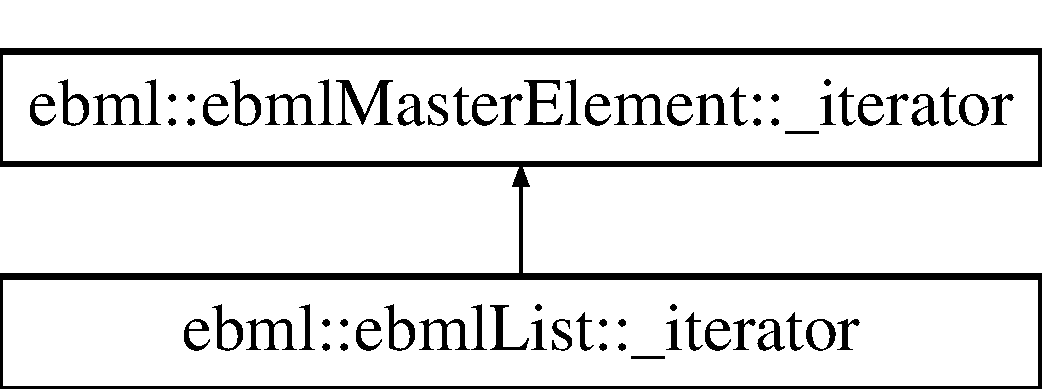
\includegraphics[height=2.000000cm]{classebml_1_1ebmlList_1_1__iterator}
\end{center}
\end{figure}
\subsection*{Public Member Functions}
\begin{DoxyCompactItemize}
\item 
\mbox{\hyperlink{classebml_1_1ebmlList_1_1__iterator_a5a1d3e19e8cc65dd7e298fb289b6eaa2}{\+\_\+iterator}} ()
\item 
virtual \mbox{\hyperlink{classebml_1_1ebmlList_1_1__iterator_ac9b20864cf56e1cf7767153ec53eefc0}{$\sim$\+\_\+iterator}} ()
\item 
\mbox{\hyperlink{classebml_1_1ebmlMasterElement_1_1__iterator}{ebml\+Master\+Element\+::\+\_\+iterator}} $\ast$ \mbox{\hyperlink{classebml_1_1ebmlList_1_1__iterator_a25602ff7d15a50f42d0acba76d38680c}{copy}} () const
\item 
const \mbox{\hyperlink{namespaceebml_adad533b7705a16bb360fe56380c5e7be}{ebml\+Element\+\_\+sp}} \& \mbox{\hyperlink{classebml_1_1ebmlList_1_1__iterator_a2fc500e854171e07d1b0e3ca9ea48fb0}{operator$\ast$}} () const
\item 
\mbox{\hyperlink{classebml_1_1ebmlMasterElement_1_1__iterator}{ebml\+Master\+Element\+::\+\_\+iterator}} \& \mbox{\hyperlink{classebml_1_1ebmlList_1_1__iterator_a48ccc42627bfcc8b681126603232f587}{operator++}} ()
\item 
\mbox{\hyperlink{classebml_1_1ebmlMasterElement_1_1__iterator}{ebml\+Master\+Element\+::\+\_\+iterator}} \& \mbox{\hyperlink{classebml_1_1ebmlList_1_1__iterator_a76134ca4a1212fcf2083fb5f3f6e7130}{operator=}} (const \mbox{\hyperlink{classebml_1_1ebmlMasterElement_1_1__iterator}{ebml\+Master\+Element\+::\+\_\+iterator}} \&)
\item 
bool \mbox{\hyperlink{classebml_1_1ebmlList_1_1__iterator_af451e7598220ae323edd778f4ca3ab21}{operator==}} (const \mbox{\hyperlink{classebml_1_1ebmlMasterElement_1_1__iterator}{ebml\+Master\+Element\+::\+\_\+iterator}} \&) const
\item 
bool \mbox{\hyperlink{classebml_1_1ebmlList_1_1__iterator_af9980e46a983daefa5bd596e88047304}{operator!=}} (const \mbox{\hyperlink{classebml_1_1ebmlMasterElement_1_1__iterator}{ebml\+Master\+Element\+::\+\_\+iterator}} \&) const
\end{DoxyCompactItemize}
\subsection*{Protected Member Functions}
\begin{DoxyCompactItemize}
\item 
\mbox{\hyperlink{classebml_1_1ebmlList_1_1__iterator_a542711e7adecf301995c4e11e08c0b66}{\+\_\+iterator}} (const \mbox{\hyperlink{namespaceebml_adad533b7705a16bb360fe56380c5e7be}{ebml\+Element\+\_\+sp}} \&elem, const std\+::vector$<$ \mbox{\hyperlink{namespaceebml_adad533b7705a16bb360fe56380c5e7be}{ebml\+Element\+\_\+sp}} $>$\+::iterator \&iter)
\end{DoxyCompactItemize}
\subsection*{Friends}
\begin{DoxyCompactItemize}
\item 
class \mbox{\hyperlink{classebml_1_1ebmlList_1_1__iterator_af371b14231393d2eef62cb562cdd6e2d}{ebml\+List}}
\item 
class \mbox{\hyperlink{classebml_1_1ebmlList_1_1__iterator_a7f678a46134f738b99dfff4aafa7fc5f}{ebml\+Master\+Element\+::iterator}}
\end{DoxyCompactItemize}


\subsection{Constructor \& Destructor Documentation}
\mbox{\Hypertarget{classebml_1_1ebmlList_1_1__iterator_a542711e7adecf301995c4e11e08c0b66}\label{classebml_1_1ebmlList_1_1__iterator_a542711e7adecf301995c4e11e08c0b66}} 
\index{ebml\+::ebml\+List\+::\+\_\+iterator@{ebml\+::ebml\+List\+::\+\_\+iterator}!\+\_\+iterator@{\+\_\+iterator}}
\index{\+\_\+iterator@{\+\_\+iterator}!ebml\+::ebml\+List\+::\+\_\+iterator@{ebml\+::ebml\+List\+::\+\_\+iterator}}
\subsubsection{\texorpdfstring{\+\_\+iterator()}{\_iterator()}\hspace{0.1cm}{\footnotesize\ttfamily [1/2]}}
{\footnotesize\ttfamily ebml\+::ebml\+List\+::\+\_\+iterator\+::\+\_\+iterator (\begin{DoxyParamCaption}\item[{const \mbox{\hyperlink{namespaceebml_adad533b7705a16bb360fe56380c5e7be}{ebml\+Element\+\_\+sp}} \&}]{elem,  }\item[{const std\+::vector$<$ \mbox{\hyperlink{namespaceebml_adad533b7705a16bb360fe56380c5e7be}{ebml\+Element\+\_\+sp}} $>$\+::iterator \&}]{iter }\end{DoxyParamCaption})\hspace{0.3cm}{\ttfamily [protected]}}

\mbox{\Hypertarget{classebml_1_1ebmlList_1_1__iterator_a5a1d3e19e8cc65dd7e298fb289b6eaa2}\label{classebml_1_1ebmlList_1_1__iterator_a5a1d3e19e8cc65dd7e298fb289b6eaa2}} 
\index{ebml\+::ebml\+List\+::\+\_\+iterator@{ebml\+::ebml\+List\+::\+\_\+iterator}!\+\_\+iterator@{\+\_\+iterator}}
\index{\+\_\+iterator@{\+\_\+iterator}!ebml\+::ebml\+List\+::\+\_\+iterator@{ebml\+::ebml\+List\+::\+\_\+iterator}}
\subsubsection{\texorpdfstring{\+\_\+iterator()}{\_iterator()}\hspace{0.1cm}{\footnotesize\ttfamily [2/2]}}
{\footnotesize\ttfamily ebml\+::ebml\+List\+::\+\_\+iterator\+::\+\_\+iterator (\begin{DoxyParamCaption}{ }\end{DoxyParamCaption})}

\mbox{\Hypertarget{classebml_1_1ebmlList_1_1__iterator_ac9b20864cf56e1cf7767153ec53eefc0}\label{classebml_1_1ebmlList_1_1__iterator_ac9b20864cf56e1cf7767153ec53eefc0}} 
\index{ebml\+::ebml\+List\+::\+\_\+iterator@{ebml\+::ebml\+List\+::\+\_\+iterator}!````~\+\_\+iterator@{$\sim$\+\_\+iterator}}
\index{````~\+\_\+iterator@{$\sim$\+\_\+iterator}!ebml\+::ebml\+List\+::\+\_\+iterator@{ebml\+::ebml\+List\+::\+\_\+iterator}}
\subsubsection{\texorpdfstring{$\sim$\+\_\+iterator()}{~\_iterator()}}
{\footnotesize\ttfamily virtual ebml\+::ebml\+List\+::\+\_\+iterator\+::$\sim$\+\_\+iterator (\begin{DoxyParamCaption}{ }\end{DoxyParamCaption})\hspace{0.3cm}{\ttfamily [virtual]}}



Reimplemented from \mbox{\hyperlink{classebml_1_1ebmlMasterElement_1_1__iterator_a499f5fe9a5dddf51dd0ca181fc98f561}{ebml\+::ebml\+Master\+Element\+::\+\_\+iterator}}.



\subsection{Member Function Documentation}
\mbox{\Hypertarget{classebml_1_1ebmlList_1_1__iterator_a25602ff7d15a50f42d0acba76d38680c}\label{classebml_1_1ebmlList_1_1__iterator_a25602ff7d15a50f42d0acba76d38680c}} 
\index{ebml\+::ebml\+List\+::\+\_\+iterator@{ebml\+::ebml\+List\+::\+\_\+iterator}!copy@{copy}}
\index{copy@{copy}!ebml\+::ebml\+List\+::\+\_\+iterator@{ebml\+::ebml\+List\+::\+\_\+iterator}}
\subsubsection{\texorpdfstring{copy()}{copy()}}
{\footnotesize\ttfamily \mbox{\hyperlink{classebml_1_1ebmlMasterElement_1_1__iterator}{ebml\+Master\+Element\+::\+\_\+iterator}}$\ast$ ebml\+::ebml\+List\+::\+\_\+iterator\+::copy (\begin{DoxyParamCaption}{ }\end{DoxyParamCaption}) const\hspace{0.3cm}{\ttfamily [virtual]}}



Implements \mbox{\hyperlink{classebml_1_1ebmlMasterElement_1_1__iterator_af9f522b6d6f34acb410add9579a35c13}{ebml\+::ebml\+Master\+Element\+::\+\_\+iterator}}.

\mbox{\Hypertarget{classebml_1_1ebmlList_1_1__iterator_af9980e46a983daefa5bd596e88047304}\label{classebml_1_1ebmlList_1_1__iterator_af9980e46a983daefa5bd596e88047304}} 
\index{ebml\+::ebml\+List\+::\+\_\+iterator@{ebml\+::ebml\+List\+::\+\_\+iterator}!operator"!=@{operator"!=}}
\index{operator"!=@{operator"!=}!ebml\+::ebml\+List\+::\+\_\+iterator@{ebml\+::ebml\+List\+::\+\_\+iterator}}
\subsubsection{\texorpdfstring{operator"!=()}{operator!=()}}
{\footnotesize\ttfamily bool ebml\+::ebml\+List\+::\+\_\+iterator\+::operator!= (\begin{DoxyParamCaption}\item[{const \mbox{\hyperlink{classebml_1_1ebmlMasterElement_1_1__iterator}{ebml\+Master\+Element\+::\+\_\+iterator}} \&}]{ }\end{DoxyParamCaption}) const\hspace{0.3cm}{\ttfamily [virtual]}}



Implements \mbox{\hyperlink{classebml_1_1ebmlMasterElement_1_1__iterator_aef9e45972d70a546942f9de73af40dc2}{ebml\+::ebml\+Master\+Element\+::\+\_\+iterator}}.

\mbox{\Hypertarget{classebml_1_1ebmlList_1_1__iterator_a2fc500e854171e07d1b0e3ca9ea48fb0}\label{classebml_1_1ebmlList_1_1__iterator_a2fc500e854171e07d1b0e3ca9ea48fb0}} 
\index{ebml\+::ebml\+List\+::\+\_\+iterator@{ebml\+::ebml\+List\+::\+\_\+iterator}!operator$\ast$@{operator$\ast$}}
\index{operator$\ast$@{operator$\ast$}!ebml\+::ebml\+List\+::\+\_\+iterator@{ebml\+::ebml\+List\+::\+\_\+iterator}}
\subsubsection{\texorpdfstring{operator$\ast$()}{operator*()}}
{\footnotesize\ttfamily const \mbox{\hyperlink{namespaceebml_adad533b7705a16bb360fe56380c5e7be}{ebml\+Element\+\_\+sp}}\& ebml\+::ebml\+List\+::\+\_\+iterator\+::operator$\ast$ (\begin{DoxyParamCaption}{ }\end{DoxyParamCaption}) const\hspace{0.3cm}{\ttfamily [virtual]}}



Implements \mbox{\hyperlink{classebml_1_1ebmlMasterElement_1_1__iterator_a3275ab5cdba37d79dd323879598f4f5d}{ebml\+::ebml\+Master\+Element\+::\+\_\+iterator}}.

\mbox{\Hypertarget{classebml_1_1ebmlList_1_1__iterator_a48ccc42627bfcc8b681126603232f587}\label{classebml_1_1ebmlList_1_1__iterator_a48ccc42627bfcc8b681126603232f587}} 
\index{ebml\+::ebml\+List\+::\+\_\+iterator@{ebml\+::ebml\+List\+::\+\_\+iterator}!operator++@{operator++}}
\index{operator++@{operator++}!ebml\+::ebml\+List\+::\+\_\+iterator@{ebml\+::ebml\+List\+::\+\_\+iterator}}
\subsubsection{\texorpdfstring{operator++()}{operator++()}}
{\footnotesize\ttfamily \mbox{\hyperlink{classebml_1_1ebmlMasterElement_1_1__iterator}{ebml\+Master\+Element\+::\+\_\+iterator}}\& ebml\+::ebml\+List\+::\+\_\+iterator\+::operator++ (\begin{DoxyParamCaption}{ }\end{DoxyParamCaption})\hspace{0.3cm}{\ttfamily [virtual]}}



Implements \mbox{\hyperlink{classebml_1_1ebmlMasterElement_1_1__iterator_ab77210fd0e481e1bb5b8563f7bd8142b}{ebml\+::ebml\+Master\+Element\+::\+\_\+iterator}}.

\mbox{\Hypertarget{classebml_1_1ebmlList_1_1__iterator_a76134ca4a1212fcf2083fb5f3f6e7130}\label{classebml_1_1ebmlList_1_1__iterator_a76134ca4a1212fcf2083fb5f3f6e7130}} 
\index{ebml\+::ebml\+List\+::\+\_\+iterator@{ebml\+::ebml\+List\+::\+\_\+iterator}!operator=@{operator=}}
\index{operator=@{operator=}!ebml\+::ebml\+List\+::\+\_\+iterator@{ebml\+::ebml\+List\+::\+\_\+iterator}}
\subsubsection{\texorpdfstring{operator=()}{operator=()}}
{\footnotesize\ttfamily \mbox{\hyperlink{classebml_1_1ebmlMasterElement_1_1__iterator}{ebml\+Master\+Element\+::\+\_\+iterator}}\& ebml\+::ebml\+List\+::\+\_\+iterator\+::operator= (\begin{DoxyParamCaption}\item[{const \mbox{\hyperlink{classebml_1_1ebmlMasterElement_1_1__iterator}{ebml\+Master\+Element\+::\+\_\+iterator}} \&}]{ }\end{DoxyParamCaption})\hspace{0.3cm}{\ttfamily [virtual]}}



Implements \mbox{\hyperlink{classebml_1_1ebmlMasterElement_1_1__iterator_a849c5027957fa1a022de0417aea1ad9e}{ebml\+::ebml\+Master\+Element\+::\+\_\+iterator}}.

\mbox{\Hypertarget{classebml_1_1ebmlList_1_1__iterator_af451e7598220ae323edd778f4ca3ab21}\label{classebml_1_1ebmlList_1_1__iterator_af451e7598220ae323edd778f4ca3ab21}} 
\index{ebml\+::ebml\+List\+::\+\_\+iterator@{ebml\+::ebml\+List\+::\+\_\+iterator}!operator==@{operator==}}
\index{operator==@{operator==}!ebml\+::ebml\+List\+::\+\_\+iterator@{ebml\+::ebml\+List\+::\+\_\+iterator}}
\subsubsection{\texorpdfstring{operator==()}{operator==()}}
{\footnotesize\ttfamily bool ebml\+::ebml\+List\+::\+\_\+iterator\+::operator== (\begin{DoxyParamCaption}\item[{const \mbox{\hyperlink{classebml_1_1ebmlMasterElement_1_1__iterator}{ebml\+Master\+Element\+::\+\_\+iterator}} \&}]{ }\end{DoxyParamCaption}) const\hspace{0.3cm}{\ttfamily [virtual]}}



Implements \mbox{\hyperlink{classebml_1_1ebmlMasterElement_1_1__iterator_ab0b53665f686e2ae379b275110ea3c95}{ebml\+::ebml\+Master\+Element\+::\+\_\+iterator}}.



\subsection{Friends And Related Function Documentation}
\mbox{\Hypertarget{classebml_1_1ebmlList_1_1__iterator_af371b14231393d2eef62cb562cdd6e2d}\label{classebml_1_1ebmlList_1_1__iterator_af371b14231393d2eef62cb562cdd6e2d}} 
\index{ebml\+::ebml\+List\+::\+\_\+iterator@{ebml\+::ebml\+List\+::\+\_\+iterator}!ebml\+List@{ebml\+List}}
\index{ebml\+List@{ebml\+List}!ebml\+::ebml\+List\+::\+\_\+iterator@{ebml\+::ebml\+List\+::\+\_\+iterator}}
\subsubsection{\texorpdfstring{ebml\+List}{ebmlList}}
{\footnotesize\ttfamily friend class \mbox{\hyperlink{classebml_1_1ebmlList}{ebml\+List}}\hspace{0.3cm}{\ttfamily [friend]}}

\mbox{\Hypertarget{classebml_1_1ebmlList_1_1__iterator_a7f678a46134f738b99dfff4aafa7fc5f}\label{classebml_1_1ebmlList_1_1__iterator_a7f678a46134f738b99dfff4aafa7fc5f}} 
\index{ebml\+::ebml\+List\+::\+\_\+iterator@{ebml\+::ebml\+List\+::\+\_\+iterator}!ebml\+Master\+Element\+::iterator@{ebml\+Master\+Element\+::iterator}}
\index{ebml\+Master\+Element\+::iterator@{ebml\+Master\+Element\+::iterator}!ebml\+::ebml\+List\+::\+\_\+iterator@{ebml\+::ebml\+List\+::\+\_\+iterator}}
\subsubsection{\texorpdfstring{ebml\+Master\+Element\+::iterator}{ebmlMasterElement::iterator}}
{\footnotesize\ttfamily friend class \mbox{\hyperlink{classebml_1_1ebmlMasterElement_1_1iterator}{ebml\+Master\+Element\+::iterator}}\hspace{0.3cm}{\ttfamily [friend]}}



The documentation for this class was generated from the following file\+:\begin{DoxyCompactItemize}
\item 
include/libebml\+\_\+ng/masterelement/\mbox{\hyperlink{list_8h}{list.\+h}}\end{DoxyCompactItemize}

\hypertarget{classebml_1_1ebmlPair_1_1__iterator}{}\section{ebml\+:\+:ebml\+Pair$<$ T $>$\+:\+:\+\_\+iterator Class Reference}
\label{classebml_1_1ebmlPair_1_1__iterator}\index{ebml\+::ebml\+Pair$<$ T $>$\+::\+\_\+iterator@{ebml\+::ebml\+Pair$<$ T $>$\+::\+\_\+iterator}}


{\ttfamily \#include $<$map.\+h$>$}

Inheritance diagram for ebml\+:\+:ebml\+Pair$<$ T $>$\+:\+:\+\_\+iterator\+:\begin{figure}[H]
\begin{center}
\leavevmode
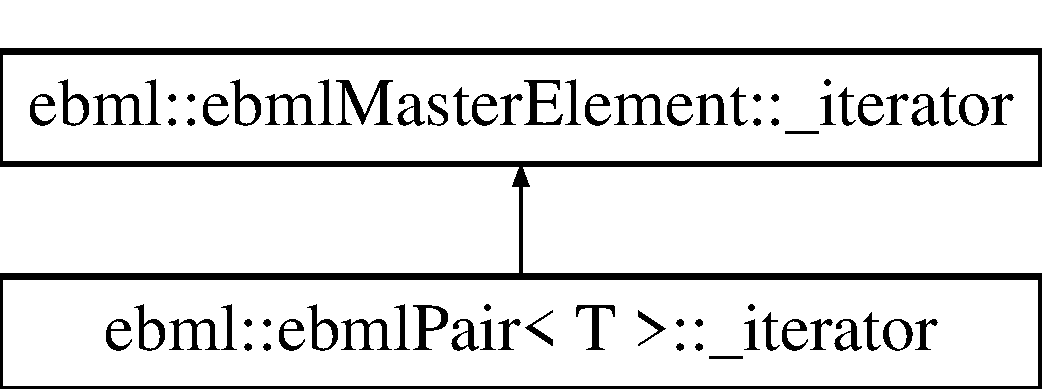
\includegraphics[height=2.000000cm]{classebml_1_1ebmlPair_1_1__iterator}
\end{center}
\end{figure}
\subsection*{Public Member Functions}
\begin{DoxyCompactItemize}
\item 
\mbox{\hyperlink{classebml_1_1ebmlPair_1_1__iterator_abbf56e96ab5f9bd6acb7b69a2efe2d38}{\+\_\+iterator}} ()
\item 
virtual \mbox{\hyperlink{classebml_1_1ebmlPair_1_1__iterator_a03a93396a9ebfae5a550f76eeaed0fb5}{$\sim$\+\_\+iterator}} ()
\item 
\mbox{\hyperlink{classebml_1_1ebmlMasterElement_1_1__iterator}{ebml\+Master\+Element\+::\+\_\+iterator}} $\ast$ \mbox{\hyperlink{classebml_1_1ebmlPair_1_1__iterator_a3f2945c8bbd6b161be18969c9a6ec260}{copy}} () const
\item 
const \mbox{\hyperlink{namespaceebml_adad533b7705a16bb360fe56380c5e7be}{ebml\+Element\+\_\+sp}} \& \mbox{\hyperlink{classebml_1_1ebmlPair_1_1__iterator_ae7f85d6a25b93280837766d206574604}{operator$\ast$}} () const
\item 
\mbox{\hyperlink{classebml_1_1ebmlMasterElement_1_1__iterator}{ebml\+Master\+Element\+::\+\_\+iterator}} \& \mbox{\hyperlink{classebml_1_1ebmlPair_1_1__iterator_a72dd1b1a818c44cc855f9340f3acbbe5}{operator++}} ()
\item 
\mbox{\hyperlink{classebml_1_1ebmlMasterElement_1_1__iterator}{ebml\+Master\+Element\+::\+\_\+iterator}} \& \mbox{\hyperlink{classebml_1_1ebmlPair_1_1__iterator_a2a77d98449db2fb4840d122f15da99be}{operator=}} (const \mbox{\hyperlink{classebml_1_1ebmlMasterElement_1_1__iterator}{ebml\+Master\+Element\+::\+\_\+iterator}} \&)
\item 
bool \mbox{\hyperlink{classebml_1_1ebmlPair_1_1__iterator_a82853adf042b58f9432861852b33ac64}{operator==}} (const \mbox{\hyperlink{classebml_1_1ebmlMasterElement_1_1__iterator}{ebml\+Master\+Element\+::\+\_\+iterator}} \&) const
\item 
bool \mbox{\hyperlink{classebml_1_1ebmlPair_1_1__iterator_a110f4b90bc4234c0e8f78160126e9baa}{operator!=}} (const \mbox{\hyperlink{classebml_1_1ebmlMasterElement_1_1__iterator}{ebml\+Master\+Element\+::\+\_\+iterator}} \&) const
\end{DoxyCompactItemize}
\subsection*{Protected Member Functions}
\begin{DoxyCompactItemize}
\item 
\mbox{\hyperlink{classebml_1_1ebmlPair_1_1__iterator_a857b4dbf1193d6f844780fd2a8a72f73}{\+\_\+iterator}} (const \mbox{\hyperlink{namespaceebml_a15439f6031c0f4ced33b9ab5e28af120}{ebml\+Pair\+\_\+sp}}$<$ T $>$ \&elem, unsigned char pos)
\item 
\mbox{\hyperlink{classebml_1_1ebmlPair_1_1__iterator_ae46c70f189bfe5ebb7859ce3175488bd}{\+\_\+iterator}} (\mbox{\hyperlink{namespaceebml_a15439f6031c0f4ced33b9ab5e28af120}{ebml\+Pair\+\_\+sp}}$<$ T $>$ \&\&elem, unsigned char pos)
\end{DoxyCompactItemize}
\subsection*{Friends}
\begin{DoxyCompactItemize}
\item 
class \mbox{\hyperlink{classebml_1_1ebmlPair_1_1__iterator_ad1db4b5395f31070d1be2d251ee85e02}{ebml\+Pair$<$ T $>$}}
\item 
class \mbox{\hyperlink{classebml_1_1ebmlPair_1_1__iterator_a7f678a46134f738b99dfff4aafa7fc5f}{ebml\+Master\+Element\+::iterator}}
\end{DoxyCompactItemize}


\subsection{Constructor \& Destructor Documentation}
\mbox{\Hypertarget{classebml_1_1ebmlPair_1_1__iterator_a857b4dbf1193d6f844780fd2a8a72f73}\label{classebml_1_1ebmlPair_1_1__iterator_a857b4dbf1193d6f844780fd2a8a72f73}} 
\index{ebml\+::ebml\+Pair\+::\+\_\+iterator@{ebml\+::ebml\+Pair\+::\+\_\+iterator}!\+\_\+iterator@{\+\_\+iterator}}
\index{\+\_\+iterator@{\+\_\+iterator}!ebml\+::ebml\+Pair\+::\+\_\+iterator@{ebml\+::ebml\+Pair\+::\+\_\+iterator}}
\subsubsection{\texorpdfstring{\+\_\+iterator()}{\_iterator()}\hspace{0.1cm}{\footnotesize\ttfamily [1/3]}}
{\footnotesize\ttfamily template$<$typename T $>$ \\
\mbox{\hyperlink{classebml_1_1ebmlPair}{ebml\+::ebml\+Pair}}$<$ T $>$\+::\+\_\+iterator\+::\+\_\+iterator (\begin{DoxyParamCaption}\item[{const \mbox{\hyperlink{namespaceebml_a15439f6031c0f4ced33b9ab5e28af120}{ebml\+Pair\+\_\+sp}}$<$ T $>$ \&}]{elem,  }\item[{unsigned char}]{pos }\end{DoxyParamCaption})\hspace{0.3cm}{\ttfamily [protected]}}

\mbox{\Hypertarget{classebml_1_1ebmlPair_1_1__iterator_ae46c70f189bfe5ebb7859ce3175488bd}\label{classebml_1_1ebmlPair_1_1__iterator_ae46c70f189bfe5ebb7859ce3175488bd}} 
\index{ebml\+::ebml\+Pair\+::\+\_\+iterator@{ebml\+::ebml\+Pair\+::\+\_\+iterator}!\+\_\+iterator@{\+\_\+iterator}}
\index{\+\_\+iterator@{\+\_\+iterator}!ebml\+::ebml\+Pair\+::\+\_\+iterator@{ebml\+::ebml\+Pair\+::\+\_\+iterator}}
\subsubsection{\texorpdfstring{\+\_\+iterator()}{\_iterator()}\hspace{0.1cm}{\footnotesize\ttfamily [2/3]}}
{\footnotesize\ttfamily template$<$typename T $>$ \\
\mbox{\hyperlink{classebml_1_1ebmlPair}{ebml\+::ebml\+Pair}}$<$ T $>$\+::\+\_\+iterator\+::\+\_\+iterator (\begin{DoxyParamCaption}\item[{\mbox{\hyperlink{namespaceebml_a15439f6031c0f4ced33b9ab5e28af120}{ebml\+Pair\+\_\+sp}}$<$ T $>$ \&\&}]{elem,  }\item[{unsigned char}]{pos }\end{DoxyParamCaption})\hspace{0.3cm}{\ttfamily [protected]}}

\mbox{\Hypertarget{classebml_1_1ebmlPair_1_1__iterator_abbf56e96ab5f9bd6acb7b69a2efe2d38}\label{classebml_1_1ebmlPair_1_1__iterator_abbf56e96ab5f9bd6acb7b69a2efe2d38}} 
\index{ebml\+::ebml\+Pair\+::\+\_\+iterator@{ebml\+::ebml\+Pair\+::\+\_\+iterator}!\+\_\+iterator@{\+\_\+iterator}}
\index{\+\_\+iterator@{\+\_\+iterator}!ebml\+::ebml\+Pair\+::\+\_\+iterator@{ebml\+::ebml\+Pair\+::\+\_\+iterator}}
\subsubsection{\texorpdfstring{\+\_\+iterator()}{\_iterator()}\hspace{0.1cm}{\footnotesize\ttfamily [3/3]}}
{\footnotesize\ttfamily template$<$typename T $>$ \\
\mbox{\hyperlink{classebml_1_1ebmlPair}{ebml\+::ebml\+Pair}}$<$ T $>$\+::\+\_\+iterator\+::\+\_\+iterator (\begin{DoxyParamCaption}{ }\end{DoxyParamCaption})}

\mbox{\Hypertarget{classebml_1_1ebmlPair_1_1__iterator_a03a93396a9ebfae5a550f76eeaed0fb5}\label{classebml_1_1ebmlPair_1_1__iterator_a03a93396a9ebfae5a550f76eeaed0fb5}} 
\index{ebml\+::ebml\+Pair\+::\+\_\+iterator@{ebml\+::ebml\+Pair\+::\+\_\+iterator}!````~\+\_\+iterator@{$\sim$\+\_\+iterator}}
\index{````~\+\_\+iterator@{$\sim$\+\_\+iterator}!ebml\+::ebml\+Pair\+::\+\_\+iterator@{ebml\+::ebml\+Pair\+::\+\_\+iterator}}
\subsubsection{\texorpdfstring{$\sim$\+\_\+iterator()}{~\_iterator()}}
{\footnotesize\ttfamily template$<$typename T $>$ \\
virtual \mbox{\hyperlink{classebml_1_1ebmlPair}{ebml\+::ebml\+Pair}}$<$ T $>$\+::\+\_\+iterator\+::$\sim$\+\_\+iterator (\begin{DoxyParamCaption}{ }\end{DoxyParamCaption})\hspace{0.3cm}{\ttfamily [virtual]}}



Reimplemented from \mbox{\hyperlink{classebml_1_1ebmlMasterElement_1_1__iterator_a499f5fe9a5dddf51dd0ca181fc98f561}{ebml\+::ebml\+Master\+Element\+::\+\_\+iterator}}.



\subsection{Member Function Documentation}
\mbox{\Hypertarget{classebml_1_1ebmlPair_1_1__iterator_a3f2945c8bbd6b161be18969c9a6ec260}\label{classebml_1_1ebmlPair_1_1__iterator_a3f2945c8bbd6b161be18969c9a6ec260}} 
\index{ebml\+::ebml\+Pair\+::\+\_\+iterator@{ebml\+::ebml\+Pair\+::\+\_\+iterator}!copy@{copy}}
\index{copy@{copy}!ebml\+::ebml\+Pair\+::\+\_\+iterator@{ebml\+::ebml\+Pair\+::\+\_\+iterator}}
\subsubsection{\texorpdfstring{copy()}{copy()}}
{\footnotesize\ttfamily template$<$typename T $>$ \\
\mbox{\hyperlink{classebml_1_1ebmlMasterElement_1_1__iterator}{ebml\+Master\+Element\+::\+\_\+iterator}}$\ast$ \mbox{\hyperlink{classebml_1_1ebmlPair}{ebml\+::ebml\+Pair}}$<$ T $>$\+::\+\_\+iterator\+::copy (\begin{DoxyParamCaption}{ }\end{DoxyParamCaption}) const\hspace{0.3cm}{\ttfamily [virtual]}}



Implements \mbox{\hyperlink{classebml_1_1ebmlMasterElement_1_1__iterator_af9f522b6d6f34acb410add9579a35c13}{ebml\+::ebml\+Master\+Element\+::\+\_\+iterator}}.

\mbox{\Hypertarget{classebml_1_1ebmlPair_1_1__iterator_a110f4b90bc4234c0e8f78160126e9baa}\label{classebml_1_1ebmlPair_1_1__iterator_a110f4b90bc4234c0e8f78160126e9baa}} 
\index{ebml\+::ebml\+Pair\+::\+\_\+iterator@{ebml\+::ebml\+Pair\+::\+\_\+iterator}!operator"!=@{operator"!=}}
\index{operator"!=@{operator"!=}!ebml\+::ebml\+Pair\+::\+\_\+iterator@{ebml\+::ebml\+Pair\+::\+\_\+iterator}}
\subsubsection{\texorpdfstring{operator"!=()}{operator!=()}}
{\footnotesize\ttfamily template$<$typename T $>$ \\
bool \mbox{\hyperlink{classebml_1_1ebmlPair}{ebml\+::ebml\+Pair}}$<$ T $>$\+::\+\_\+iterator\+::operator!= (\begin{DoxyParamCaption}\item[{const \mbox{\hyperlink{classebml_1_1ebmlMasterElement_1_1__iterator}{ebml\+Master\+Element\+::\+\_\+iterator}} \&}]{ }\end{DoxyParamCaption}) const\hspace{0.3cm}{\ttfamily [virtual]}}



Implements \mbox{\hyperlink{classebml_1_1ebmlMasterElement_1_1__iterator_aef9e45972d70a546942f9de73af40dc2}{ebml\+::ebml\+Master\+Element\+::\+\_\+iterator}}.

\mbox{\Hypertarget{classebml_1_1ebmlPair_1_1__iterator_ae7f85d6a25b93280837766d206574604}\label{classebml_1_1ebmlPair_1_1__iterator_ae7f85d6a25b93280837766d206574604}} 
\index{ebml\+::ebml\+Pair\+::\+\_\+iterator@{ebml\+::ebml\+Pair\+::\+\_\+iterator}!operator$\ast$@{operator$\ast$}}
\index{operator$\ast$@{operator$\ast$}!ebml\+::ebml\+Pair\+::\+\_\+iterator@{ebml\+::ebml\+Pair\+::\+\_\+iterator}}
\subsubsection{\texorpdfstring{operator$\ast$()}{operator*()}}
{\footnotesize\ttfamily template$<$typename T $>$ \\
const \mbox{\hyperlink{namespaceebml_adad533b7705a16bb360fe56380c5e7be}{ebml\+Element\+\_\+sp}}\& \mbox{\hyperlink{classebml_1_1ebmlPair}{ebml\+::ebml\+Pair}}$<$ T $>$\+::\+\_\+iterator\+::operator$\ast$ (\begin{DoxyParamCaption}{ }\end{DoxyParamCaption}) const\hspace{0.3cm}{\ttfamily [virtual]}}



Implements \mbox{\hyperlink{classebml_1_1ebmlMasterElement_1_1__iterator_a3275ab5cdba37d79dd323879598f4f5d}{ebml\+::ebml\+Master\+Element\+::\+\_\+iterator}}.

\mbox{\Hypertarget{classebml_1_1ebmlPair_1_1__iterator_a72dd1b1a818c44cc855f9340f3acbbe5}\label{classebml_1_1ebmlPair_1_1__iterator_a72dd1b1a818c44cc855f9340f3acbbe5}} 
\index{ebml\+::ebml\+Pair\+::\+\_\+iterator@{ebml\+::ebml\+Pair\+::\+\_\+iterator}!operator++@{operator++}}
\index{operator++@{operator++}!ebml\+::ebml\+Pair\+::\+\_\+iterator@{ebml\+::ebml\+Pair\+::\+\_\+iterator}}
\subsubsection{\texorpdfstring{operator++()}{operator++()}}
{\footnotesize\ttfamily template$<$typename T $>$ \\
\mbox{\hyperlink{classebml_1_1ebmlMasterElement_1_1__iterator}{ebml\+Master\+Element\+::\+\_\+iterator}}\& \mbox{\hyperlink{classebml_1_1ebmlPair}{ebml\+::ebml\+Pair}}$<$ T $>$\+::\+\_\+iterator\+::operator++ (\begin{DoxyParamCaption}{ }\end{DoxyParamCaption})\hspace{0.3cm}{\ttfamily [virtual]}}



Implements \mbox{\hyperlink{classebml_1_1ebmlMasterElement_1_1__iterator_ab77210fd0e481e1bb5b8563f7bd8142b}{ebml\+::ebml\+Master\+Element\+::\+\_\+iterator}}.

\mbox{\Hypertarget{classebml_1_1ebmlPair_1_1__iterator_a2a77d98449db2fb4840d122f15da99be}\label{classebml_1_1ebmlPair_1_1__iterator_a2a77d98449db2fb4840d122f15da99be}} 
\index{ebml\+::ebml\+Pair\+::\+\_\+iterator@{ebml\+::ebml\+Pair\+::\+\_\+iterator}!operator=@{operator=}}
\index{operator=@{operator=}!ebml\+::ebml\+Pair\+::\+\_\+iterator@{ebml\+::ebml\+Pair\+::\+\_\+iterator}}
\subsubsection{\texorpdfstring{operator=()}{operator=()}}
{\footnotesize\ttfamily template$<$typename T $>$ \\
\mbox{\hyperlink{classebml_1_1ebmlMasterElement_1_1__iterator}{ebml\+Master\+Element\+::\+\_\+iterator}}\& \mbox{\hyperlink{classebml_1_1ebmlPair}{ebml\+::ebml\+Pair}}$<$ T $>$\+::\+\_\+iterator\+::operator= (\begin{DoxyParamCaption}\item[{const \mbox{\hyperlink{classebml_1_1ebmlMasterElement_1_1__iterator}{ebml\+Master\+Element\+::\+\_\+iterator}} \&}]{ }\end{DoxyParamCaption})\hspace{0.3cm}{\ttfamily [virtual]}}



Implements \mbox{\hyperlink{classebml_1_1ebmlMasterElement_1_1__iterator_a849c5027957fa1a022de0417aea1ad9e}{ebml\+::ebml\+Master\+Element\+::\+\_\+iterator}}.

\mbox{\Hypertarget{classebml_1_1ebmlPair_1_1__iterator_a82853adf042b58f9432861852b33ac64}\label{classebml_1_1ebmlPair_1_1__iterator_a82853adf042b58f9432861852b33ac64}} 
\index{ebml\+::ebml\+Pair\+::\+\_\+iterator@{ebml\+::ebml\+Pair\+::\+\_\+iterator}!operator==@{operator==}}
\index{operator==@{operator==}!ebml\+::ebml\+Pair\+::\+\_\+iterator@{ebml\+::ebml\+Pair\+::\+\_\+iterator}}
\subsubsection{\texorpdfstring{operator==()}{operator==()}}
{\footnotesize\ttfamily template$<$typename T $>$ \\
bool \mbox{\hyperlink{classebml_1_1ebmlPair}{ebml\+::ebml\+Pair}}$<$ T $>$\+::\+\_\+iterator\+::operator== (\begin{DoxyParamCaption}\item[{const \mbox{\hyperlink{classebml_1_1ebmlMasterElement_1_1__iterator}{ebml\+Master\+Element\+::\+\_\+iterator}} \&}]{ }\end{DoxyParamCaption}) const\hspace{0.3cm}{\ttfamily [virtual]}}



Implements \mbox{\hyperlink{classebml_1_1ebmlMasterElement_1_1__iterator_ab0b53665f686e2ae379b275110ea3c95}{ebml\+::ebml\+Master\+Element\+::\+\_\+iterator}}.



\subsection{Friends And Related Function Documentation}
\mbox{\Hypertarget{classebml_1_1ebmlPair_1_1__iterator_a7f678a46134f738b99dfff4aafa7fc5f}\label{classebml_1_1ebmlPair_1_1__iterator_a7f678a46134f738b99dfff4aafa7fc5f}} 
\index{ebml\+::ebml\+Pair\+::\+\_\+iterator@{ebml\+::ebml\+Pair\+::\+\_\+iterator}!ebml\+Master\+Element\+::iterator@{ebml\+Master\+Element\+::iterator}}
\index{ebml\+Master\+Element\+::iterator@{ebml\+Master\+Element\+::iterator}!ebml\+::ebml\+Pair\+::\+\_\+iterator@{ebml\+::ebml\+Pair\+::\+\_\+iterator}}
\subsubsection{\texorpdfstring{ebml\+Master\+Element\+::iterator}{ebmlMasterElement::iterator}}
{\footnotesize\ttfamily template$<$typename T $>$ \\
friend class \mbox{\hyperlink{classebml_1_1ebmlMasterElement_1_1iterator}{ebml\+Master\+Element\+::iterator}}\hspace{0.3cm}{\ttfamily [friend]}}

\mbox{\Hypertarget{classebml_1_1ebmlPair_1_1__iterator_ad1db4b5395f31070d1be2d251ee85e02}\label{classebml_1_1ebmlPair_1_1__iterator_ad1db4b5395f31070d1be2d251ee85e02}} 
\index{ebml\+::ebml\+Pair\+::\+\_\+iterator@{ebml\+::ebml\+Pair\+::\+\_\+iterator}!ebml\+Pair$<$ T $>$@{ebml\+Pair$<$ T $>$}}
\index{ebml\+Pair$<$ T $>$@{ebml\+Pair$<$ T $>$}!ebml\+::ebml\+Pair\+::\+\_\+iterator@{ebml\+::ebml\+Pair\+::\+\_\+iterator}}
\subsubsection{\texorpdfstring{ebml\+Pair$<$ T $>$}{ebmlPair< T >}}
{\footnotesize\ttfamily template$<$typename T $>$ \\
friend class \mbox{\hyperlink{classebml_1_1ebmlPair}{ebml\+Pair}}$<$ T $>$\hspace{0.3cm}{\ttfamily [friend]}}



The documentation for this class was generated from the following file\+:\begin{DoxyCompactItemize}
\item 
include/libebml\+\_\+ng/masterelement/\mbox{\hyperlink{map_8h}{map.\+h}}\end{DoxyCompactItemize}

\hypertarget{classebml_1_1ebmlMap_1_1__iterator}{}\section{ebml\+:\+:ebml\+Map$<$ K, H, E, A $>$\+:\+:\+\_\+iterator Class Reference}
\label{classebml_1_1ebmlMap_1_1__iterator}\index{ebml\+::ebml\+Map$<$ K, H, E, A $>$\+::\+\_\+iterator@{ebml\+::ebml\+Map$<$ K, H, E, A $>$\+::\+\_\+iterator}}


{\ttfamily \#include $<$map.\+h$>$}

Inheritance diagram for ebml\+:\+:ebml\+Map$<$ K, H, E, A $>$\+:\+:\+\_\+iterator\+:\begin{figure}[H]
\begin{center}
\leavevmode
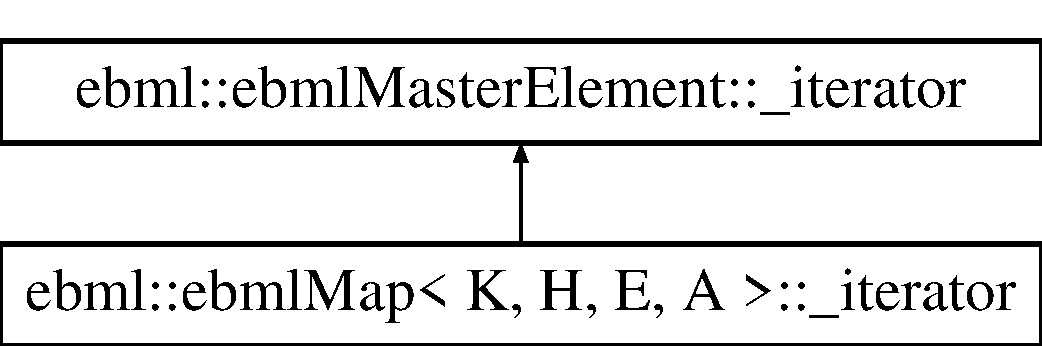
\includegraphics[height=2.000000cm]{classebml_1_1ebmlMap_1_1__iterator}
\end{center}
\end{figure}
\subsection*{Public Member Functions}
\begin{DoxyCompactItemize}
\item 
\mbox{\hyperlink{classebml_1_1ebmlMap_1_1__iterator_a4cbcb4c34c842171b9b628c681c4e77a}{\+\_\+iterator}} ()
\item 
virtual \mbox{\hyperlink{classebml_1_1ebmlMap_1_1__iterator_a276c17f3a552f25f09735ffb6679fabd}{$\sim$\+\_\+iterator}} ()
\item 
\mbox{\hyperlink{classebml_1_1ebmlMasterElement_1_1__iterator}{ebml\+Master\+Element\+::\+\_\+iterator}} $\ast$ \mbox{\hyperlink{classebml_1_1ebmlMap_1_1__iterator_a4ae1670445455ff5b27e5b3e2bc93142}{copy}} () const
\item 
const \mbox{\hyperlink{namespaceebml_adad533b7705a16bb360fe56380c5e7be}{ebml\+Element\+\_\+sp}} \& \mbox{\hyperlink{classebml_1_1ebmlMap_1_1__iterator_aedbcdd2c78b42961a1f7478fec5080a4}{operator$\ast$}} () const
\item 
\mbox{\hyperlink{classebml_1_1ebmlMasterElement_1_1__iterator}{ebml\+Master\+Element\+::\+\_\+iterator}} \& \mbox{\hyperlink{classebml_1_1ebmlMap_1_1__iterator_aa35aad1b71670402a6152989c9b0cf6b}{operator++}} ()
\item 
\mbox{\hyperlink{classebml_1_1ebmlMasterElement_1_1__iterator}{ebml\+Master\+Element\+::\+\_\+iterator}} \& \mbox{\hyperlink{classebml_1_1ebmlMap_1_1__iterator_af9aa2621f2b2d78c75a473b3c4b94fc4}{operator=}} (const \mbox{\hyperlink{classebml_1_1ebmlMasterElement_1_1__iterator}{ebml\+Master\+Element\+::\+\_\+iterator}} \&)
\item 
bool \mbox{\hyperlink{classebml_1_1ebmlMap_1_1__iterator_abda291b4e2305234d8215d4a3b03e7a5}{operator==}} (const \mbox{\hyperlink{classebml_1_1ebmlMasterElement_1_1__iterator}{ebml\+Master\+Element\+::\+\_\+iterator}} \&) const
\item 
bool \mbox{\hyperlink{classebml_1_1ebmlMap_1_1__iterator_a42189d25979dab96126d411ab83a3849}{operator!=}} (const \mbox{\hyperlink{classebml_1_1ebmlMasterElement_1_1__iterator}{ebml\+Master\+Element\+::\+\_\+iterator}} \&) const
\end{DoxyCompactItemize}
\subsection*{Protected Member Functions}
\begin{DoxyCompactItemize}
\item 
\mbox{\hyperlink{classebml_1_1ebmlMap_1_1__iterator_afcab3ed0bb37c020c39a09098bc751a8}{\+\_\+iterator}} (const \mbox{\hyperlink{namespaceebml_adad533b7705a16bb360fe56380c5e7be}{ebml\+Element\+\_\+sp}} \&elem, const typename std\+::unordered\+\_\+map$<$ K, \mbox{\hyperlink{namespaceebml_adad533b7705a16bb360fe56380c5e7be}{ebml\+Element\+\_\+sp}}, H, E, A $>$\+::\mbox{\hyperlink{classebml_1_1ebmlMasterElement_1_1iterator}{iterator}} \&iter)
\item 
\mbox{\hyperlink{classebml_1_1ebmlMap_1_1__iterator_a0664de1ae97c95b30c3b08b40c4b8b6e}{\+\_\+iterator}} (\mbox{\hyperlink{namespaceebml_adad533b7705a16bb360fe56380c5e7be}{ebml\+Element\+\_\+sp}} \&\&elem, typename std\+::unordered\+\_\+map$<$ K, \mbox{\hyperlink{namespaceebml_adad533b7705a16bb360fe56380c5e7be}{ebml\+Element\+\_\+sp}}, H, E, A $>$\+::\mbox{\hyperlink{classebml_1_1ebmlMasterElement_1_1iterator}{iterator}} \&\&iter)
\end{DoxyCompactItemize}
\subsection*{Friends}
\begin{DoxyCompactItemize}
\item 
class \mbox{\hyperlink{classebml_1_1ebmlMap_1_1__iterator_a691e480013452ea48661a61746fd1b5c}{ebml\+Map$<$ K, H, E, A $>$}}
\item 
class \mbox{\hyperlink{classebml_1_1ebmlMap_1_1__iterator_a7f678a46134f738b99dfff4aafa7fc5f}{ebml\+Master\+Element\+::iterator}}
\end{DoxyCompactItemize}


\subsection{Constructor \& Destructor Documentation}
\mbox{\Hypertarget{classebml_1_1ebmlMap_1_1__iterator_afcab3ed0bb37c020c39a09098bc751a8}\label{classebml_1_1ebmlMap_1_1__iterator_afcab3ed0bb37c020c39a09098bc751a8}} 
\index{ebml\+::ebml\+Map\+::\+\_\+iterator@{ebml\+::ebml\+Map\+::\+\_\+iterator}!\+\_\+iterator@{\+\_\+iterator}}
\index{\+\_\+iterator@{\+\_\+iterator}!ebml\+::ebml\+Map\+::\+\_\+iterator@{ebml\+::ebml\+Map\+::\+\_\+iterator}}
\subsubsection{\texorpdfstring{\+\_\+iterator()}{\_iterator()}\hspace{0.1cm}{\footnotesize\ttfamily [1/3]}}
{\footnotesize\ttfamily template$<$typename K , typename H , typename E , typename A $>$ \\
\mbox{\hyperlink{classebml_1_1ebmlMap}{ebml\+::ebml\+Map}}$<$ K, H, E, A $>$\+::\+\_\+iterator\+::\+\_\+iterator (\begin{DoxyParamCaption}\item[{const \mbox{\hyperlink{namespaceebml_adad533b7705a16bb360fe56380c5e7be}{ebml\+Element\+\_\+sp}} \&}]{elem,  }\item[{const typename std\+::unordered\+\_\+map$<$ K, \mbox{\hyperlink{namespaceebml_adad533b7705a16bb360fe56380c5e7be}{ebml\+Element\+\_\+sp}}, H, E, A $>$\+::\mbox{\hyperlink{classebml_1_1ebmlMasterElement_1_1iterator}{iterator}} \&}]{iter }\end{DoxyParamCaption})\hspace{0.3cm}{\ttfamily [protected]}}

\mbox{\Hypertarget{classebml_1_1ebmlMap_1_1__iterator_a0664de1ae97c95b30c3b08b40c4b8b6e}\label{classebml_1_1ebmlMap_1_1__iterator_a0664de1ae97c95b30c3b08b40c4b8b6e}} 
\index{ebml\+::ebml\+Map\+::\+\_\+iterator@{ebml\+::ebml\+Map\+::\+\_\+iterator}!\+\_\+iterator@{\+\_\+iterator}}
\index{\+\_\+iterator@{\+\_\+iterator}!ebml\+::ebml\+Map\+::\+\_\+iterator@{ebml\+::ebml\+Map\+::\+\_\+iterator}}
\subsubsection{\texorpdfstring{\+\_\+iterator()}{\_iterator()}\hspace{0.1cm}{\footnotesize\ttfamily [2/3]}}
{\footnotesize\ttfamily template$<$typename K , typename H , typename E , typename A $>$ \\
\mbox{\hyperlink{classebml_1_1ebmlMap}{ebml\+::ebml\+Map}}$<$ K, H, E, A $>$\+::\+\_\+iterator\+::\+\_\+iterator (\begin{DoxyParamCaption}\item[{\mbox{\hyperlink{namespaceebml_adad533b7705a16bb360fe56380c5e7be}{ebml\+Element\+\_\+sp}} \&\&}]{elem,  }\item[{typename std\+::unordered\+\_\+map$<$ K, \mbox{\hyperlink{namespaceebml_adad533b7705a16bb360fe56380c5e7be}{ebml\+Element\+\_\+sp}}, H, E, A $>$\+::\mbox{\hyperlink{classebml_1_1ebmlMasterElement_1_1iterator}{iterator}} \&\&}]{iter }\end{DoxyParamCaption})\hspace{0.3cm}{\ttfamily [protected]}}

\mbox{\Hypertarget{classebml_1_1ebmlMap_1_1__iterator_a4cbcb4c34c842171b9b628c681c4e77a}\label{classebml_1_1ebmlMap_1_1__iterator_a4cbcb4c34c842171b9b628c681c4e77a}} 
\index{ebml\+::ebml\+Map\+::\+\_\+iterator@{ebml\+::ebml\+Map\+::\+\_\+iterator}!\+\_\+iterator@{\+\_\+iterator}}
\index{\+\_\+iterator@{\+\_\+iterator}!ebml\+::ebml\+Map\+::\+\_\+iterator@{ebml\+::ebml\+Map\+::\+\_\+iterator}}
\subsubsection{\texorpdfstring{\+\_\+iterator()}{\_iterator()}\hspace{0.1cm}{\footnotesize\ttfamily [3/3]}}
{\footnotesize\ttfamily template$<$typename K , typename H , typename E , typename A $>$ \\
\mbox{\hyperlink{classebml_1_1ebmlMap}{ebml\+::ebml\+Map}}$<$ K, H, E, A $>$\+::\+\_\+iterator\+::\+\_\+iterator (\begin{DoxyParamCaption}{ }\end{DoxyParamCaption})}

\mbox{\Hypertarget{classebml_1_1ebmlMap_1_1__iterator_a276c17f3a552f25f09735ffb6679fabd}\label{classebml_1_1ebmlMap_1_1__iterator_a276c17f3a552f25f09735ffb6679fabd}} 
\index{ebml\+::ebml\+Map\+::\+\_\+iterator@{ebml\+::ebml\+Map\+::\+\_\+iterator}!````~\+\_\+iterator@{$\sim$\+\_\+iterator}}
\index{````~\+\_\+iterator@{$\sim$\+\_\+iterator}!ebml\+::ebml\+Map\+::\+\_\+iterator@{ebml\+::ebml\+Map\+::\+\_\+iterator}}
\subsubsection{\texorpdfstring{$\sim$\+\_\+iterator()}{~\_iterator()}}
{\footnotesize\ttfamily template$<$typename K , typename H , typename E , typename A $>$ \\
virtual \mbox{\hyperlink{classebml_1_1ebmlMap}{ebml\+::ebml\+Map}}$<$ K, H, E, A $>$\+::\+\_\+iterator\+::$\sim$\+\_\+iterator (\begin{DoxyParamCaption}{ }\end{DoxyParamCaption})\hspace{0.3cm}{\ttfamily [virtual]}}



Reimplemented from \mbox{\hyperlink{classebml_1_1ebmlMasterElement_1_1__iterator_a499f5fe9a5dddf51dd0ca181fc98f561}{ebml\+::ebml\+Master\+Element\+::\+\_\+iterator}}.



\subsection{Member Function Documentation}
\mbox{\Hypertarget{classebml_1_1ebmlMap_1_1__iterator_a4ae1670445455ff5b27e5b3e2bc93142}\label{classebml_1_1ebmlMap_1_1__iterator_a4ae1670445455ff5b27e5b3e2bc93142}} 
\index{ebml\+::ebml\+Map\+::\+\_\+iterator@{ebml\+::ebml\+Map\+::\+\_\+iterator}!copy@{copy}}
\index{copy@{copy}!ebml\+::ebml\+Map\+::\+\_\+iterator@{ebml\+::ebml\+Map\+::\+\_\+iterator}}
\subsubsection{\texorpdfstring{copy()}{copy()}}
{\footnotesize\ttfamily template$<$typename K , typename H , typename E , typename A $>$ \\
\mbox{\hyperlink{classebml_1_1ebmlMasterElement_1_1__iterator}{ebml\+Master\+Element\+::\+\_\+iterator}}$\ast$ \mbox{\hyperlink{classebml_1_1ebmlMap}{ebml\+::ebml\+Map}}$<$ K, H, E, A $>$\+::\+\_\+iterator\+::copy (\begin{DoxyParamCaption}{ }\end{DoxyParamCaption}) const\hspace{0.3cm}{\ttfamily [virtual]}}



Implements \mbox{\hyperlink{classebml_1_1ebmlMasterElement_1_1__iterator_af9f522b6d6f34acb410add9579a35c13}{ebml\+::ebml\+Master\+Element\+::\+\_\+iterator}}.

\mbox{\Hypertarget{classebml_1_1ebmlMap_1_1__iterator_a42189d25979dab96126d411ab83a3849}\label{classebml_1_1ebmlMap_1_1__iterator_a42189d25979dab96126d411ab83a3849}} 
\index{ebml\+::ebml\+Map\+::\+\_\+iterator@{ebml\+::ebml\+Map\+::\+\_\+iterator}!operator"!=@{operator"!=}}
\index{operator"!=@{operator"!=}!ebml\+::ebml\+Map\+::\+\_\+iterator@{ebml\+::ebml\+Map\+::\+\_\+iterator}}
\subsubsection{\texorpdfstring{operator"!=()}{operator!=()}}
{\footnotesize\ttfamily template$<$typename K , typename H , typename E , typename A $>$ \\
bool \mbox{\hyperlink{classebml_1_1ebmlMap}{ebml\+::ebml\+Map}}$<$ K, H, E, A $>$\+::\+\_\+iterator\+::operator!= (\begin{DoxyParamCaption}\item[{const \mbox{\hyperlink{classebml_1_1ebmlMasterElement_1_1__iterator}{ebml\+Master\+Element\+::\+\_\+iterator}} \&}]{ }\end{DoxyParamCaption}) const\hspace{0.3cm}{\ttfamily [virtual]}}



Implements \mbox{\hyperlink{classebml_1_1ebmlMasterElement_1_1__iterator_aef9e45972d70a546942f9de73af40dc2}{ebml\+::ebml\+Master\+Element\+::\+\_\+iterator}}.

\mbox{\Hypertarget{classebml_1_1ebmlMap_1_1__iterator_aedbcdd2c78b42961a1f7478fec5080a4}\label{classebml_1_1ebmlMap_1_1__iterator_aedbcdd2c78b42961a1f7478fec5080a4}} 
\index{ebml\+::ebml\+Map\+::\+\_\+iterator@{ebml\+::ebml\+Map\+::\+\_\+iterator}!operator$\ast$@{operator$\ast$}}
\index{operator$\ast$@{operator$\ast$}!ebml\+::ebml\+Map\+::\+\_\+iterator@{ebml\+::ebml\+Map\+::\+\_\+iterator}}
\subsubsection{\texorpdfstring{operator$\ast$()}{operator*()}}
{\footnotesize\ttfamily template$<$typename K , typename H , typename E , typename A $>$ \\
const \mbox{\hyperlink{namespaceebml_adad533b7705a16bb360fe56380c5e7be}{ebml\+Element\+\_\+sp}}\& \mbox{\hyperlink{classebml_1_1ebmlMap}{ebml\+::ebml\+Map}}$<$ K, H, E, A $>$\+::\+\_\+iterator\+::operator$\ast$ (\begin{DoxyParamCaption}{ }\end{DoxyParamCaption}) const\hspace{0.3cm}{\ttfamily [virtual]}}



Implements \mbox{\hyperlink{classebml_1_1ebmlMasterElement_1_1__iterator_a3275ab5cdba37d79dd323879598f4f5d}{ebml\+::ebml\+Master\+Element\+::\+\_\+iterator}}.

\mbox{\Hypertarget{classebml_1_1ebmlMap_1_1__iterator_aa35aad1b71670402a6152989c9b0cf6b}\label{classebml_1_1ebmlMap_1_1__iterator_aa35aad1b71670402a6152989c9b0cf6b}} 
\index{ebml\+::ebml\+Map\+::\+\_\+iterator@{ebml\+::ebml\+Map\+::\+\_\+iterator}!operator++@{operator++}}
\index{operator++@{operator++}!ebml\+::ebml\+Map\+::\+\_\+iterator@{ebml\+::ebml\+Map\+::\+\_\+iterator}}
\subsubsection{\texorpdfstring{operator++()}{operator++()}}
{\footnotesize\ttfamily template$<$typename K , typename H , typename E , typename A $>$ \\
\mbox{\hyperlink{classebml_1_1ebmlMasterElement_1_1__iterator}{ebml\+Master\+Element\+::\+\_\+iterator}}\& \mbox{\hyperlink{classebml_1_1ebmlMap}{ebml\+::ebml\+Map}}$<$ K, H, E, A $>$\+::\+\_\+iterator\+::operator++ (\begin{DoxyParamCaption}{ }\end{DoxyParamCaption})\hspace{0.3cm}{\ttfamily [virtual]}}



Implements \mbox{\hyperlink{classebml_1_1ebmlMasterElement_1_1__iterator_ab77210fd0e481e1bb5b8563f7bd8142b}{ebml\+::ebml\+Master\+Element\+::\+\_\+iterator}}.

\mbox{\Hypertarget{classebml_1_1ebmlMap_1_1__iterator_af9aa2621f2b2d78c75a473b3c4b94fc4}\label{classebml_1_1ebmlMap_1_1__iterator_af9aa2621f2b2d78c75a473b3c4b94fc4}} 
\index{ebml\+::ebml\+Map\+::\+\_\+iterator@{ebml\+::ebml\+Map\+::\+\_\+iterator}!operator=@{operator=}}
\index{operator=@{operator=}!ebml\+::ebml\+Map\+::\+\_\+iterator@{ebml\+::ebml\+Map\+::\+\_\+iterator}}
\subsubsection{\texorpdfstring{operator=()}{operator=()}}
{\footnotesize\ttfamily template$<$typename K , typename H , typename E , typename A $>$ \\
\mbox{\hyperlink{classebml_1_1ebmlMasterElement_1_1__iterator}{ebml\+Master\+Element\+::\+\_\+iterator}}\& \mbox{\hyperlink{classebml_1_1ebmlMap}{ebml\+::ebml\+Map}}$<$ K, H, E, A $>$\+::\+\_\+iterator\+::operator= (\begin{DoxyParamCaption}\item[{const \mbox{\hyperlink{classebml_1_1ebmlMasterElement_1_1__iterator}{ebml\+Master\+Element\+::\+\_\+iterator}} \&}]{ }\end{DoxyParamCaption})\hspace{0.3cm}{\ttfamily [virtual]}}



Implements \mbox{\hyperlink{classebml_1_1ebmlMasterElement_1_1__iterator_a849c5027957fa1a022de0417aea1ad9e}{ebml\+::ebml\+Master\+Element\+::\+\_\+iterator}}.

\mbox{\Hypertarget{classebml_1_1ebmlMap_1_1__iterator_abda291b4e2305234d8215d4a3b03e7a5}\label{classebml_1_1ebmlMap_1_1__iterator_abda291b4e2305234d8215d4a3b03e7a5}} 
\index{ebml\+::ebml\+Map\+::\+\_\+iterator@{ebml\+::ebml\+Map\+::\+\_\+iterator}!operator==@{operator==}}
\index{operator==@{operator==}!ebml\+::ebml\+Map\+::\+\_\+iterator@{ebml\+::ebml\+Map\+::\+\_\+iterator}}
\subsubsection{\texorpdfstring{operator==()}{operator==()}}
{\footnotesize\ttfamily template$<$typename K , typename H , typename E , typename A $>$ \\
bool \mbox{\hyperlink{classebml_1_1ebmlMap}{ebml\+::ebml\+Map}}$<$ K, H, E, A $>$\+::\+\_\+iterator\+::operator== (\begin{DoxyParamCaption}\item[{const \mbox{\hyperlink{classebml_1_1ebmlMasterElement_1_1__iterator}{ebml\+Master\+Element\+::\+\_\+iterator}} \&}]{ }\end{DoxyParamCaption}) const\hspace{0.3cm}{\ttfamily [virtual]}}



Implements \mbox{\hyperlink{classebml_1_1ebmlMasterElement_1_1__iterator_ab0b53665f686e2ae379b275110ea3c95}{ebml\+::ebml\+Master\+Element\+::\+\_\+iterator}}.



\subsection{Friends And Related Function Documentation}
\mbox{\Hypertarget{classebml_1_1ebmlMap_1_1__iterator_a691e480013452ea48661a61746fd1b5c}\label{classebml_1_1ebmlMap_1_1__iterator_a691e480013452ea48661a61746fd1b5c}} 
\index{ebml\+::ebml\+Map\+::\+\_\+iterator@{ebml\+::ebml\+Map\+::\+\_\+iterator}!ebml\+Map$<$ K, H, E, A $>$@{ebml\+Map$<$ K, H, E, A $>$}}
\index{ebml\+Map$<$ K, H, E, A $>$@{ebml\+Map$<$ K, H, E, A $>$}!ebml\+::ebml\+Map\+::\+\_\+iterator@{ebml\+::ebml\+Map\+::\+\_\+iterator}}
\subsubsection{\texorpdfstring{ebml\+Map$<$ K, H, E, A $>$}{ebmlMap< K, H, E, A >}}
{\footnotesize\ttfamily template$<$typename K , typename H , typename E , typename A $>$ \\
friend class \mbox{\hyperlink{classebml_1_1ebmlMap}{ebml\+Map}}$<$ K, H, E, A $>$\hspace{0.3cm}{\ttfamily [friend]}}

\mbox{\Hypertarget{classebml_1_1ebmlMap_1_1__iterator_a7f678a46134f738b99dfff4aafa7fc5f}\label{classebml_1_1ebmlMap_1_1__iterator_a7f678a46134f738b99dfff4aafa7fc5f}} 
\index{ebml\+::ebml\+Map\+::\+\_\+iterator@{ebml\+::ebml\+Map\+::\+\_\+iterator}!ebml\+Master\+Element\+::iterator@{ebml\+Master\+Element\+::iterator}}
\index{ebml\+Master\+Element\+::iterator@{ebml\+Master\+Element\+::iterator}!ebml\+::ebml\+Map\+::\+\_\+iterator@{ebml\+::ebml\+Map\+::\+\_\+iterator}}
\subsubsection{\texorpdfstring{ebml\+Master\+Element\+::iterator}{ebmlMasterElement::iterator}}
{\footnotesize\ttfamily template$<$typename K , typename H , typename E , typename A $>$ \\
friend class \mbox{\hyperlink{classebml_1_1ebmlMasterElement_1_1iterator}{ebml\+Master\+Element\+::iterator}}\hspace{0.3cm}{\ttfamily [friend]}}



The documentation for this class was generated from the following file\+:\begin{DoxyCompactItemize}
\item 
include/libebml\+\_\+ng/masterelement/\mbox{\hyperlink{map_8h}{map.\+h}}\end{DoxyCompactItemize}

\hypertarget{classebml_1_1ebmlMultiSlot_1_1__iterator}{}\section{ebml\+:\+:ebml\+Multi\+Slot\+:\+:\+\_\+iterator Class Reference}
\label{classebml_1_1ebmlMultiSlot_1_1__iterator}\index{ebml\+::ebml\+Multi\+Slot\+::\+\_\+iterator@{ebml\+::ebml\+Multi\+Slot\+::\+\_\+iterator}}


{\ttfamily \#include $<$multislot.\+h$>$}

Inheritance diagram for ebml\+:\+:ebml\+Multi\+Slot\+:\+:\+\_\+iterator\+:\begin{figure}[H]
\begin{center}
\leavevmode
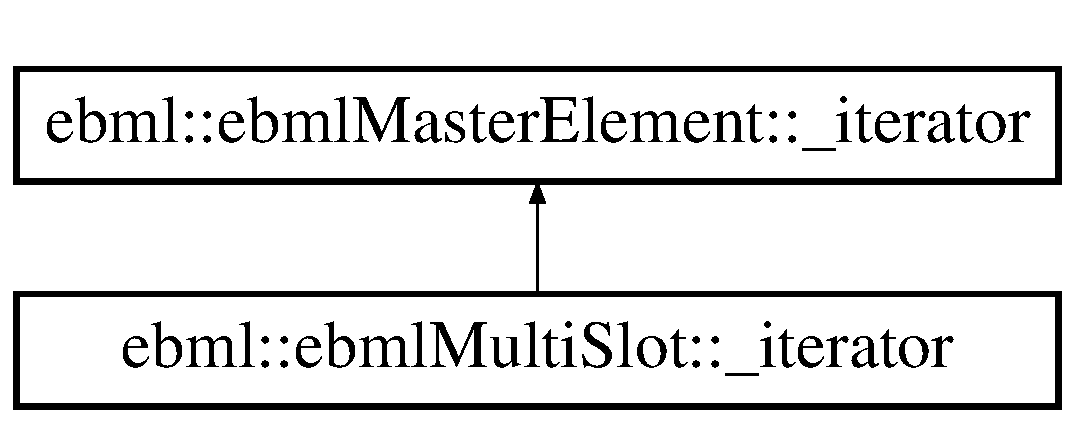
\includegraphics[height=2.000000cm]{classebml_1_1ebmlMultiSlot_1_1__iterator}
\end{center}
\end{figure}
\subsection*{Public Member Functions}
\begin{DoxyCompactItemize}
\item 
\mbox{\hyperlink{classebml_1_1ebmlMultiSlot_1_1__iterator_a9a5bb54966d95ad5ea80373761494523}{\+\_\+iterator}} ()
\item 
virtual \mbox{\hyperlink{classebml_1_1ebmlMultiSlot_1_1__iterator_a1d4b6ffee0d593ee22ac312d61d99d16}{$\sim$\+\_\+iterator}} ()
\item 
\mbox{\hyperlink{classebml_1_1ebmlMasterElement_1_1__iterator}{ebml\+Master\+Element\+::\+\_\+iterator}} $\ast$ \mbox{\hyperlink{classebml_1_1ebmlMultiSlot_1_1__iterator_a7f26180e096089e0a14986731bc04326}{copy}} () const
\item 
const \mbox{\hyperlink{namespaceebml_adad533b7705a16bb360fe56380c5e7be}{ebml\+Element\+\_\+sp}} \& \mbox{\hyperlink{classebml_1_1ebmlMultiSlot_1_1__iterator_a3baa39c32ce95c538e8fee957d683e50}{operator$\ast$}} () const
\item 
\mbox{\hyperlink{classebml_1_1ebmlMasterElement_1_1__iterator}{ebml\+Master\+Element\+::\+\_\+iterator}} \& \mbox{\hyperlink{classebml_1_1ebmlMultiSlot_1_1__iterator_a59e3bf809115c2ef28cbaf05c0d78afd}{operator++}} ()
\item 
\mbox{\hyperlink{classebml_1_1ebmlMasterElement_1_1__iterator}{ebml\+Master\+Element\+::\+\_\+iterator}} \& \mbox{\hyperlink{classebml_1_1ebmlMultiSlot_1_1__iterator_ae21fb8ce6820c3540dedf14eee28d24a}{operator=}} (const \mbox{\hyperlink{classebml_1_1ebmlMasterElement_1_1__iterator}{ebml\+Master\+Element\+::\+\_\+iterator}} \&)
\item 
bool \mbox{\hyperlink{classebml_1_1ebmlMultiSlot_1_1__iterator_a306e7fd7a564d17febbb08a75dd95b36}{operator==}} (const \mbox{\hyperlink{classebml_1_1ebmlMasterElement_1_1__iterator}{ebml\+Master\+Element\+::\+\_\+iterator}} \&) const
\item 
bool \mbox{\hyperlink{classebml_1_1ebmlMultiSlot_1_1__iterator_a250650c2080db120a29383e5f588feeb}{operator!=}} (const \mbox{\hyperlink{classebml_1_1ebmlMasterElement_1_1__iterator}{ebml\+Master\+Element\+::\+\_\+iterator}} \&) const
\end{DoxyCompactItemize}
\subsection*{Protected Member Functions}
\begin{DoxyCompactItemize}
\item 
\mbox{\hyperlink{classebml_1_1ebmlMultiSlot_1_1__iterator_ad4c2e04a5cf2b94c9abb9a14bf64f017}{\+\_\+iterator}} (const \mbox{\hyperlink{namespaceebml_adad533b7705a16bb360fe56380c5e7be}{ebml\+Element\+\_\+sp}} \&elem, const std\+::vector$<$ \+\_\+slot\+\_\+t $>$\+::\mbox{\hyperlink{classebml_1_1ebmlMasterElement_1_1iterator}{iterator}} \&slotiter, const std\+::vector$<$ \+\_\+slot\+\_\+t $>$\+::\mbox{\hyperlink{classebml_1_1ebmlMasterElement_1_1iterator}{iterator}} \&slotiterend, const \mbox{\hyperlink{classebml_1_1slot__t_1_1iterator}{slot\+\_\+t\+::iterator}} \&iter, const \mbox{\hyperlink{classebml_1_1slot__t_1_1iterator}{slot\+\_\+t\+::iterator}} \&iterend)
\item 
\mbox{\hyperlink{classebml_1_1ebmlMultiSlot_1_1__iterator_a74075a206c4d25bb335a79a4b471ef0b}{\+\_\+iterator}} (\mbox{\hyperlink{namespaceebml_adad533b7705a16bb360fe56380c5e7be}{ebml\+Element\+\_\+sp}} \&\&elem, std\+::vector$<$ \+\_\+slot\+\_\+t $>$\+::\mbox{\hyperlink{classebml_1_1ebmlMasterElement_1_1iterator}{iterator}} \&\&slotiter, std\+::vector$<$ \+\_\+slot\+\_\+t $>$\+::\mbox{\hyperlink{classebml_1_1ebmlMasterElement_1_1iterator}{iterator}} \&\&slotiterend, \mbox{\hyperlink{classebml_1_1slot__t_1_1iterator}{slot\+\_\+t\+::iterator}} \&\&iter, \mbox{\hyperlink{classebml_1_1slot__t_1_1iterator}{slot\+\_\+t\+::iterator}} \&\&iterend)
\end{DoxyCompactItemize}
\subsection*{Friends}
\begin{DoxyCompactItemize}
\item 
class \mbox{\hyperlink{classebml_1_1ebmlMultiSlot_1_1__iterator_ab14eb6c5a125d7276a7b4b5b6573428b}{ebml\+Multi\+Slot}}
\item 
class \mbox{\hyperlink{classebml_1_1ebmlMultiSlot_1_1__iterator_a7f678a46134f738b99dfff4aafa7fc5f}{ebml\+Master\+Element\+::iterator}}
\item 
class \mbox{\hyperlink{classebml_1_1ebmlMultiSlot_1_1__iterator_a6c39add7736de258762e32f3536f516a}{std\+::shared\+\_\+ptr$<$ \+\_\+iterator $>$}}
\end{DoxyCompactItemize}


\subsection{Constructor \& Destructor Documentation}
\mbox{\Hypertarget{classebml_1_1ebmlMultiSlot_1_1__iterator_ad4c2e04a5cf2b94c9abb9a14bf64f017}\label{classebml_1_1ebmlMultiSlot_1_1__iterator_ad4c2e04a5cf2b94c9abb9a14bf64f017}} 
\index{ebml\+::ebml\+Multi\+Slot\+::\+\_\+iterator@{ebml\+::ebml\+Multi\+Slot\+::\+\_\+iterator}!\+\_\+iterator@{\+\_\+iterator}}
\index{\+\_\+iterator@{\+\_\+iterator}!ebml\+::ebml\+Multi\+Slot\+::\+\_\+iterator@{ebml\+::ebml\+Multi\+Slot\+::\+\_\+iterator}}
\subsubsection{\texorpdfstring{\+\_\+iterator()}{\_iterator()}\hspace{0.1cm}{\footnotesize\ttfamily [1/3]}}
{\footnotesize\ttfamily ebml\+::ebml\+Multi\+Slot\+::\+\_\+iterator\+::\+\_\+iterator (\begin{DoxyParamCaption}\item[{const \mbox{\hyperlink{namespaceebml_adad533b7705a16bb360fe56380c5e7be}{ebml\+Element\+\_\+sp}} \&}]{elem,  }\item[{const std\+::vector$<$ \+\_\+slot\+\_\+t $>$\+::\mbox{\hyperlink{classebml_1_1ebmlMasterElement_1_1iterator}{iterator}} \&}]{slotiter,  }\item[{const std\+::vector$<$ \+\_\+slot\+\_\+t $>$\+::\mbox{\hyperlink{classebml_1_1ebmlMasterElement_1_1iterator}{iterator}} \&}]{slotiterend,  }\item[{const \mbox{\hyperlink{classebml_1_1slot__t_1_1iterator}{slot\+\_\+t\+::iterator}} \&}]{iter,  }\item[{const \mbox{\hyperlink{classebml_1_1slot__t_1_1iterator}{slot\+\_\+t\+::iterator}} \&}]{iterend }\end{DoxyParamCaption})\hspace{0.3cm}{\ttfamily [protected]}}

\mbox{\Hypertarget{classebml_1_1ebmlMultiSlot_1_1__iterator_a74075a206c4d25bb335a79a4b471ef0b}\label{classebml_1_1ebmlMultiSlot_1_1__iterator_a74075a206c4d25bb335a79a4b471ef0b}} 
\index{ebml\+::ebml\+Multi\+Slot\+::\+\_\+iterator@{ebml\+::ebml\+Multi\+Slot\+::\+\_\+iterator}!\+\_\+iterator@{\+\_\+iterator}}
\index{\+\_\+iterator@{\+\_\+iterator}!ebml\+::ebml\+Multi\+Slot\+::\+\_\+iterator@{ebml\+::ebml\+Multi\+Slot\+::\+\_\+iterator}}
\subsubsection{\texorpdfstring{\+\_\+iterator()}{\_iterator()}\hspace{0.1cm}{\footnotesize\ttfamily [2/3]}}
{\footnotesize\ttfamily ebml\+::ebml\+Multi\+Slot\+::\+\_\+iterator\+::\+\_\+iterator (\begin{DoxyParamCaption}\item[{\mbox{\hyperlink{namespaceebml_adad533b7705a16bb360fe56380c5e7be}{ebml\+Element\+\_\+sp}} \&\&}]{elem,  }\item[{std\+::vector$<$ \+\_\+slot\+\_\+t $>$\+::\mbox{\hyperlink{classebml_1_1ebmlMasterElement_1_1iterator}{iterator}} \&\&}]{slotiter,  }\item[{std\+::vector$<$ \+\_\+slot\+\_\+t $>$\+::\mbox{\hyperlink{classebml_1_1ebmlMasterElement_1_1iterator}{iterator}} \&\&}]{slotiterend,  }\item[{\mbox{\hyperlink{classebml_1_1slot__t_1_1iterator}{slot\+\_\+t\+::iterator}} \&\&}]{iter,  }\item[{\mbox{\hyperlink{classebml_1_1slot__t_1_1iterator}{slot\+\_\+t\+::iterator}} \&\&}]{iterend }\end{DoxyParamCaption})\hspace{0.3cm}{\ttfamily [protected]}}

\mbox{\Hypertarget{classebml_1_1ebmlMultiSlot_1_1__iterator_a9a5bb54966d95ad5ea80373761494523}\label{classebml_1_1ebmlMultiSlot_1_1__iterator_a9a5bb54966d95ad5ea80373761494523}} 
\index{ebml\+::ebml\+Multi\+Slot\+::\+\_\+iterator@{ebml\+::ebml\+Multi\+Slot\+::\+\_\+iterator}!\+\_\+iterator@{\+\_\+iterator}}
\index{\+\_\+iterator@{\+\_\+iterator}!ebml\+::ebml\+Multi\+Slot\+::\+\_\+iterator@{ebml\+::ebml\+Multi\+Slot\+::\+\_\+iterator}}
\subsubsection{\texorpdfstring{\+\_\+iterator()}{\_iterator()}\hspace{0.1cm}{\footnotesize\ttfamily [3/3]}}
{\footnotesize\ttfamily ebml\+::ebml\+Multi\+Slot\+::\+\_\+iterator\+::\+\_\+iterator (\begin{DoxyParamCaption}{ }\end{DoxyParamCaption})}

\mbox{\Hypertarget{classebml_1_1ebmlMultiSlot_1_1__iterator_a1d4b6ffee0d593ee22ac312d61d99d16}\label{classebml_1_1ebmlMultiSlot_1_1__iterator_a1d4b6ffee0d593ee22ac312d61d99d16}} 
\index{ebml\+::ebml\+Multi\+Slot\+::\+\_\+iterator@{ebml\+::ebml\+Multi\+Slot\+::\+\_\+iterator}!````~\+\_\+iterator@{$\sim$\+\_\+iterator}}
\index{````~\+\_\+iterator@{$\sim$\+\_\+iterator}!ebml\+::ebml\+Multi\+Slot\+::\+\_\+iterator@{ebml\+::ebml\+Multi\+Slot\+::\+\_\+iterator}}
\subsubsection{\texorpdfstring{$\sim$\+\_\+iterator()}{~\_iterator()}}
{\footnotesize\ttfamily virtual ebml\+::ebml\+Multi\+Slot\+::\+\_\+iterator\+::$\sim$\+\_\+iterator (\begin{DoxyParamCaption}{ }\end{DoxyParamCaption})\hspace{0.3cm}{\ttfamily [virtual]}}



Reimplemented from \mbox{\hyperlink{classebml_1_1ebmlMasterElement_1_1__iterator_a499f5fe9a5dddf51dd0ca181fc98f561}{ebml\+::ebml\+Master\+Element\+::\+\_\+iterator}}.



\subsection{Member Function Documentation}
\mbox{\Hypertarget{classebml_1_1ebmlMultiSlot_1_1__iterator_a7f26180e096089e0a14986731bc04326}\label{classebml_1_1ebmlMultiSlot_1_1__iterator_a7f26180e096089e0a14986731bc04326}} 
\index{ebml\+::ebml\+Multi\+Slot\+::\+\_\+iterator@{ebml\+::ebml\+Multi\+Slot\+::\+\_\+iterator}!copy@{copy}}
\index{copy@{copy}!ebml\+::ebml\+Multi\+Slot\+::\+\_\+iterator@{ebml\+::ebml\+Multi\+Slot\+::\+\_\+iterator}}
\subsubsection{\texorpdfstring{copy()}{copy()}}
{\footnotesize\ttfamily \mbox{\hyperlink{classebml_1_1ebmlMasterElement_1_1__iterator}{ebml\+Master\+Element\+::\+\_\+iterator}}$\ast$ ebml\+::ebml\+Multi\+Slot\+::\+\_\+iterator\+::copy (\begin{DoxyParamCaption}{ }\end{DoxyParamCaption}) const\hspace{0.3cm}{\ttfamily [virtual]}}



Implements \mbox{\hyperlink{classebml_1_1ebmlMasterElement_1_1__iterator_af9f522b6d6f34acb410add9579a35c13}{ebml\+::ebml\+Master\+Element\+::\+\_\+iterator}}.

\mbox{\Hypertarget{classebml_1_1ebmlMultiSlot_1_1__iterator_a250650c2080db120a29383e5f588feeb}\label{classebml_1_1ebmlMultiSlot_1_1__iterator_a250650c2080db120a29383e5f588feeb}} 
\index{ebml\+::ebml\+Multi\+Slot\+::\+\_\+iterator@{ebml\+::ebml\+Multi\+Slot\+::\+\_\+iterator}!operator"!=@{operator"!=}}
\index{operator"!=@{operator"!=}!ebml\+::ebml\+Multi\+Slot\+::\+\_\+iterator@{ebml\+::ebml\+Multi\+Slot\+::\+\_\+iterator}}
\subsubsection{\texorpdfstring{operator"!=()}{operator!=()}}
{\footnotesize\ttfamily bool ebml\+::ebml\+Multi\+Slot\+::\+\_\+iterator\+::operator!= (\begin{DoxyParamCaption}\item[{const \mbox{\hyperlink{classebml_1_1ebmlMasterElement_1_1__iterator}{ebml\+Master\+Element\+::\+\_\+iterator}} \&}]{ }\end{DoxyParamCaption}) const\hspace{0.3cm}{\ttfamily [virtual]}}



Implements \mbox{\hyperlink{classebml_1_1ebmlMasterElement_1_1__iterator_aef9e45972d70a546942f9de73af40dc2}{ebml\+::ebml\+Master\+Element\+::\+\_\+iterator}}.

\mbox{\Hypertarget{classebml_1_1ebmlMultiSlot_1_1__iterator_a3baa39c32ce95c538e8fee957d683e50}\label{classebml_1_1ebmlMultiSlot_1_1__iterator_a3baa39c32ce95c538e8fee957d683e50}} 
\index{ebml\+::ebml\+Multi\+Slot\+::\+\_\+iterator@{ebml\+::ebml\+Multi\+Slot\+::\+\_\+iterator}!operator$\ast$@{operator$\ast$}}
\index{operator$\ast$@{operator$\ast$}!ebml\+::ebml\+Multi\+Slot\+::\+\_\+iterator@{ebml\+::ebml\+Multi\+Slot\+::\+\_\+iterator}}
\subsubsection{\texorpdfstring{operator$\ast$()}{operator*()}}
{\footnotesize\ttfamily const \mbox{\hyperlink{namespaceebml_adad533b7705a16bb360fe56380c5e7be}{ebml\+Element\+\_\+sp}}\& ebml\+::ebml\+Multi\+Slot\+::\+\_\+iterator\+::operator$\ast$ (\begin{DoxyParamCaption}{ }\end{DoxyParamCaption}) const\hspace{0.3cm}{\ttfamily [virtual]}}



Implements \mbox{\hyperlink{classebml_1_1ebmlMasterElement_1_1__iterator_a3275ab5cdba37d79dd323879598f4f5d}{ebml\+::ebml\+Master\+Element\+::\+\_\+iterator}}.

\mbox{\Hypertarget{classebml_1_1ebmlMultiSlot_1_1__iterator_a59e3bf809115c2ef28cbaf05c0d78afd}\label{classebml_1_1ebmlMultiSlot_1_1__iterator_a59e3bf809115c2ef28cbaf05c0d78afd}} 
\index{ebml\+::ebml\+Multi\+Slot\+::\+\_\+iterator@{ebml\+::ebml\+Multi\+Slot\+::\+\_\+iterator}!operator++@{operator++}}
\index{operator++@{operator++}!ebml\+::ebml\+Multi\+Slot\+::\+\_\+iterator@{ebml\+::ebml\+Multi\+Slot\+::\+\_\+iterator}}
\subsubsection{\texorpdfstring{operator++()}{operator++()}}
{\footnotesize\ttfamily \mbox{\hyperlink{classebml_1_1ebmlMasterElement_1_1__iterator}{ebml\+Master\+Element\+::\+\_\+iterator}}\& ebml\+::ebml\+Multi\+Slot\+::\+\_\+iterator\+::operator++ (\begin{DoxyParamCaption}{ }\end{DoxyParamCaption})\hspace{0.3cm}{\ttfamily [virtual]}}



Implements \mbox{\hyperlink{classebml_1_1ebmlMasterElement_1_1__iterator_ab77210fd0e481e1bb5b8563f7bd8142b}{ebml\+::ebml\+Master\+Element\+::\+\_\+iterator}}.

\mbox{\Hypertarget{classebml_1_1ebmlMultiSlot_1_1__iterator_ae21fb8ce6820c3540dedf14eee28d24a}\label{classebml_1_1ebmlMultiSlot_1_1__iterator_ae21fb8ce6820c3540dedf14eee28d24a}} 
\index{ebml\+::ebml\+Multi\+Slot\+::\+\_\+iterator@{ebml\+::ebml\+Multi\+Slot\+::\+\_\+iterator}!operator=@{operator=}}
\index{operator=@{operator=}!ebml\+::ebml\+Multi\+Slot\+::\+\_\+iterator@{ebml\+::ebml\+Multi\+Slot\+::\+\_\+iterator}}
\subsubsection{\texorpdfstring{operator=()}{operator=()}}
{\footnotesize\ttfamily \mbox{\hyperlink{classebml_1_1ebmlMasterElement_1_1__iterator}{ebml\+Master\+Element\+::\+\_\+iterator}}\& ebml\+::ebml\+Multi\+Slot\+::\+\_\+iterator\+::operator= (\begin{DoxyParamCaption}\item[{const \mbox{\hyperlink{classebml_1_1ebmlMasterElement_1_1__iterator}{ebml\+Master\+Element\+::\+\_\+iterator}} \&}]{ }\end{DoxyParamCaption})\hspace{0.3cm}{\ttfamily [virtual]}}



Implements \mbox{\hyperlink{classebml_1_1ebmlMasterElement_1_1__iterator_a849c5027957fa1a022de0417aea1ad9e}{ebml\+::ebml\+Master\+Element\+::\+\_\+iterator}}.

\mbox{\Hypertarget{classebml_1_1ebmlMultiSlot_1_1__iterator_a306e7fd7a564d17febbb08a75dd95b36}\label{classebml_1_1ebmlMultiSlot_1_1__iterator_a306e7fd7a564d17febbb08a75dd95b36}} 
\index{ebml\+::ebml\+Multi\+Slot\+::\+\_\+iterator@{ebml\+::ebml\+Multi\+Slot\+::\+\_\+iterator}!operator==@{operator==}}
\index{operator==@{operator==}!ebml\+::ebml\+Multi\+Slot\+::\+\_\+iterator@{ebml\+::ebml\+Multi\+Slot\+::\+\_\+iterator}}
\subsubsection{\texorpdfstring{operator==()}{operator==()}}
{\footnotesize\ttfamily bool ebml\+::ebml\+Multi\+Slot\+::\+\_\+iterator\+::operator== (\begin{DoxyParamCaption}\item[{const \mbox{\hyperlink{classebml_1_1ebmlMasterElement_1_1__iterator}{ebml\+Master\+Element\+::\+\_\+iterator}} \&}]{ }\end{DoxyParamCaption}) const\hspace{0.3cm}{\ttfamily [virtual]}}



Implements \mbox{\hyperlink{classebml_1_1ebmlMasterElement_1_1__iterator_ab0b53665f686e2ae379b275110ea3c95}{ebml\+::ebml\+Master\+Element\+::\+\_\+iterator}}.



\subsection{Friends And Related Function Documentation}
\mbox{\Hypertarget{classebml_1_1ebmlMultiSlot_1_1__iterator_a7f678a46134f738b99dfff4aafa7fc5f}\label{classebml_1_1ebmlMultiSlot_1_1__iterator_a7f678a46134f738b99dfff4aafa7fc5f}} 
\index{ebml\+::ebml\+Multi\+Slot\+::\+\_\+iterator@{ebml\+::ebml\+Multi\+Slot\+::\+\_\+iterator}!ebml\+Master\+Element\+::iterator@{ebml\+Master\+Element\+::iterator}}
\index{ebml\+Master\+Element\+::iterator@{ebml\+Master\+Element\+::iterator}!ebml\+::ebml\+Multi\+Slot\+::\+\_\+iterator@{ebml\+::ebml\+Multi\+Slot\+::\+\_\+iterator}}
\subsubsection{\texorpdfstring{ebml\+Master\+Element\+::iterator}{ebmlMasterElement::iterator}}
{\footnotesize\ttfamily friend class \mbox{\hyperlink{classebml_1_1ebmlMasterElement_1_1iterator}{ebml\+Master\+Element\+::iterator}}\hspace{0.3cm}{\ttfamily [friend]}}

\mbox{\Hypertarget{classebml_1_1ebmlMultiSlot_1_1__iterator_ab14eb6c5a125d7276a7b4b5b6573428b}\label{classebml_1_1ebmlMultiSlot_1_1__iterator_ab14eb6c5a125d7276a7b4b5b6573428b}} 
\index{ebml\+::ebml\+Multi\+Slot\+::\+\_\+iterator@{ebml\+::ebml\+Multi\+Slot\+::\+\_\+iterator}!ebml\+Multi\+Slot@{ebml\+Multi\+Slot}}
\index{ebml\+Multi\+Slot@{ebml\+Multi\+Slot}!ebml\+::ebml\+Multi\+Slot\+::\+\_\+iterator@{ebml\+::ebml\+Multi\+Slot\+::\+\_\+iterator}}
\subsubsection{\texorpdfstring{ebml\+Multi\+Slot}{ebmlMultiSlot}}
{\footnotesize\ttfamily friend class \mbox{\hyperlink{classebml_1_1ebmlMultiSlot}{ebml\+Multi\+Slot}}\hspace{0.3cm}{\ttfamily [friend]}}

\mbox{\Hypertarget{classebml_1_1ebmlMultiSlot_1_1__iterator_a6c39add7736de258762e32f3536f516a}\label{classebml_1_1ebmlMultiSlot_1_1__iterator_a6c39add7736de258762e32f3536f516a}} 
\index{ebml\+::ebml\+Multi\+Slot\+::\+\_\+iterator@{ebml\+::ebml\+Multi\+Slot\+::\+\_\+iterator}!std\+::shared\+\_\+ptr$<$ \+\_\+iterator $>$@{std\+::shared\+\_\+ptr$<$ \+\_\+iterator $>$}}
\index{std\+::shared\+\_\+ptr$<$ \+\_\+iterator $>$@{std\+::shared\+\_\+ptr$<$ \+\_\+iterator $>$}!ebml\+::ebml\+Multi\+Slot\+::\+\_\+iterator@{ebml\+::ebml\+Multi\+Slot\+::\+\_\+iterator}}
\subsubsection{\texorpdfstring{std\+::shared\+\_\+ptr$<$ \+\_\+iterator $>$}{std::shared\_ptr< \_iterator >}}
{\footnotesize\ttfamily friend class std\+::shared\+\_\+ptr$<$ \mbox{\hyperlink{classebml_1_1ebmlMultiSlot_1_1__iterator}{\+\_\+iterator}} $>$\hspace{0.3cm}{\ttfamily [friend]}}



The documentation for this class was generated from the following file\+:\begin{DoxyCompactItemize}
\item 
include/libebml\+\_\+ng/masterelement/\mbox{\hyperlink{multislot_8h}{multislot.\+h}}\end{DoxyCompactItemize}

\hypertarget{classebml_1_1c__ebmlElement__l}{}\section{ebml\+:\+:c\+\_\+ebml\+Element\+\_\+l Class Reference}
\label{classebml_1_1c__ebmlElement__l}\index{ebml\+::c\+\_\+ebml\+Element\+\_\+l@{ebml\+::c\+\_\+ebml\+Element\+\_\+l}}


{\ttfamily \#include $<$base.\+h$>$}

\subsection*{Classes}
\begin{DoxyCompactItemize}
\item 
class \mbox{\hyperlink{classebml_1_1c__ebmlElement__l_1_1const__iterator}{const\+\_\+iterator}}
\end{DoxyCompactItemize}
\subsection*{Public Member Functions}
\begin{DoxyCompactItemize}
\item 
\mbox{\hyperlink{classebml_1_1c__ebmlElement__l_afad39184d6e43871e4c9c8a14e0fd969}{c\+\_\+ebml\+Element\+\_\+l}} (const \mbox{\hyperlink{namespaceebml_a1ddadd26791f273d851882653b9caf70}{ebml\+Element\+\_\+l}} \&)
\item 
\mbox{\hyperlink{classebml_1_1c__ebmlElement__l_a9d5550deb8015eafbd81eaee562eadbe}{c\+\_\+ebml\+Element\+\_\+l}} (const \mbox{\hyperlink{classebml_1_1c__ebmlElement__l}{c\+\_\+ebml\+Element\+\_\+l}} \&)
\item 
\mbox{\hyperlink{namespaceebml_a2deef4e8071531b32e3533f1bf978917}{c\+\_\+ebml\+Element\+\_\+sp}} \mbox{\hyperlink{classebml_1_1c__ebmlElement__l_ae21b42b7599179c218be4c05ea0fb07c}{front}} () const
\item 
\mbox{\hyperlink{namespaceebml_a2deef4e8071531b32e3533f1bf978917}{c\+\_\+ebml\+Element\+\_\+sp}} \mbox{\hyperlink{classebml_1_1c__ebmlElement__l_a9a3f7be3e7bb6d6c3005da1c3140247e}{back}} () const
\item 
\mbox{\hyperlink{namespaceebml_a2deef4e8071531b32e3533f1bf978917}{c\+\_\+ebml\+Element\+\_\+sp}} \mbox{\hyperlink{classebml_1_1c__ebmlElement__l_a81866f8123d15fb41d7f8e8d4e4cca41}{at}} (size\+\_\+t) const
\item 
\mbox{\hyperlink{namespaceebml_a2deef4e8071531b32e3533f1bf978917}{c\+\_\+ebml\+Element\+\_\+sp}} \mbox{\hyperlink{classebml_1_1c__ebmlElement__l_a96efd97da3095d4041f055415ab9ae6b}{operator\mbox{[}$\,$\mbox{]}}} (size\+\_\+t) const
\item 
size\+\_\+t \mbox{\hyperlink{classebml_1_1c__ebmlElement__l_adc228d5daa606faf08cb29feedee3d33}{size}} () const
\item 
bool \mbox{\hyperlink{classebml_1_1c__ebmlElement__l_a832048afabdeb9dfa373f3c8ed7c595b}{empty}} () const
\item 
\mbox{\hyperlink{classebml_1_1c__ebmlElement__l_1_1const__iterator}{const\+\_\+iterator}} \mbox{\hyperlink{classebml_1_1c__ebmlElement__l_ae6f0e1b17374fbaee1ffdac656a46496}{cbegin}} () const
\item 
\mbox{\hyperlink{classebml_1_1c__ebmlElement__l_1_1const__iterator}{const\+\_\+iterator}} \mbox{\hyperlink{classebml_1_1c__ebmlElement__l_a8bc0ed15b406c1a1144ad2fb55a195bc}{cend}} () const
\end{DoxyCompactItemize}


\subsection{Constructor \& Destructor Documentation}
\mbox{\Hypertarget{classebml_1_1c__ebmlElement__l_afad39184d6e43871e4c9c8a14e0fd969}\label{classebml_1_1c__ebmlElement__l_afad39184d6e43871e4c9c8a14e0fd969}} 
\index{ebml\+::c\+\_\+ebml\+Element\+\_\+l@{ebml\+::c\+\_\+ebml\+Element\+\_\+l}!c\+\_\+ebml\+Element\+\_\+l@{c\+\_\+ebml\+Element\+\_\+l}}
\index{c\+\_\+ebml\+Element\+\_\+l@{c\+\_\+ebml\+Element\+\_\+l}!ebml\+::c\+\_\+ebml\+Element\+\_\+l@{ebml\+::c\+\_\+ebml\+Element\+\_\+l}}
\subsubsection{\texorpdfstring{c\+\_\+ebml\+Element\+\_\+l()}{c\_ebmlElement\_l()}\hspace{0.1cm}{\footnotesize\ttfamily [1/2]}}
{\footnotesize\ttfamily ebml\+::c\+\_\+ebml\+Element\+\_\+l\+::c\+\_\+ebml\+Element\+\_\+l (\begin{DoxyParamCaption}\item[{const \mbox{\hyperlink{namespaceebml_a1ddadd26791f273d851882653b9caf70}{ebml\+Element\+\_\+l}} \&}]{ }\end{DoxyParamCaption})}

\mbox{\Hypertarget{classebml_1_1c__ebmlElement__l_a9d5550deb8015eafbd81eaee562eadbe}\label{classebml_1_1c__ebmlElement__l_a9d5550deb8015eafbd81eaee562eadbe}} 
\index{ebml\+::c\+\_\+ebml\+Element\+\_\+l@{ebml\+::c\+\_\+ebml\+Element\+\_\+l}!c\+\_\+ebml\+Element\+\_\+l@{c\+\_\+ebml\+Element\+\_\+l}}
\index{c\+\_\+ebml\+Element\+\_\+l@{c\+\_\+ebml\+Element\+\_\+l}!ebml\+::c\+\_\+ebml\+Element\+\_\+l@{ebml\+::c\+\_\+ebml\+Element\+\_\+l}}
\subsubsection{\texorpdfstring{c\+\_\+ebml\+Element\+\_\+l()}{c\_ebmlElement\_l()}\hspace{0.1cm}{\footnotesize\ttfamily [2/2]}}
{\footnotesize\ttfamily ebml\+::c\+\_\+ebml\+Element\+\_\+l\+::c\+\_\+ebml\+Element\+\_\+l (\begin{DoxyParamCaption}\item[{const \mbox{\hyperlink{classebml_1_1c__ebmlElement__l}{c\+\_\+ebml\+Element\+\_\+l}} \&}]{ }\end{DoxyParamCaption})}



\subsection{Member Function Documentation}
\mbox{\Hypertarget{classebml_1_1c__ebmlElement__l_a81866f8123d15fb41d7f8e8d4e4cca41}\label{classebml_1_1c__ebmlElement__l_a81866f8123d15fb41d7f8e8d4e4cca41}} 
\index{ebml\+::c\+\_\+ebml\+Element\+\_\+l@{ebml\+::c\+\_\+ebml\+Element\+\_\+l}!at@{at}}
\index{at@{at}!ebml\+::c\+\_\+ebml\+Element\+\_\+l@{ebml\+::c\+\_\+ebml\+Element\+\_\+l}}
\subsubsection{\texorpdfstring{at()}{at()}}
{\footnotesize\ttfamily \mbox{\hyperlink{namespaceebml_a2deef4e8071531b32e3533f1bf978917}{c\+\_\+ebml\+Element\+\_\+sp}} ebml\+::c\+\_\+ebml\+Element\+\_\+l\+::at (\begin{DoxyParamCaption}\item[{size\+\_\+t}]{ }\end{DoxyParamCaption}) const}

\mbox{\Hypertarget{classebml_1_1c__ebmlElement__l_a9a3f7be3e7bb6d6c3005da1c3140247e}\label{classebml_1_1c__ebmlElement__l_a9a3f7be3e7bb6d6c3005da1c3140247e}} 
\index{ebml\+::c\+\_\+ebml\+Element\+\_\+l@{ebml\+::c\+\_\+ebml\+Element\+\_\+l}!back@{back}}
\index{back@{back}!ebml\+::c\+\_\+ebml\+Element\+\_\+l@{ebml\+::c\+\_\+ebml\+Element\+\_\+l}}
\subsubsection{\texorpdfstring{back()}{back()}}
{\footnotesize\ttfamily \mbox{\hyperlink{namespaceebml_a2deef4e8071531b32e3533f1bf978917}{c\+\_\+ebml\+Element\+\_\+sp}} ebml\+::c\+\_\+ebml\+Element\+\_\+l\+::back (\begin{DoxyParamCaption}{ }\end{DoxyParamCaption}) const}

\mbox{\Hypertarget{classebml_1_1c__ebmlElement__l_ae6f0e1b17374fbaee1ffdac656a46496}\label{classebml_1_1c__ebmlElement__l_ae6f0e1b17374fbaee1ffdac656a46496}} 
\index{ebml\+::c\+\_\+ebml\+Element\+\_\+l@{ebml\+::c\+\_\+ebml\+Element\+\_\+l}!cbegin@{cbegin}}
\index{cbegin@{cbegin}!ebml\+::c\+\_\+ebml\+Element\+\_\+l@{ebml\+::c\+\_\+ebml\+Element\+\_\+l}}
\subsubsection{\texorpdfstring{cbegin()}{cbegin()}}
{\footnotesize\ttfamily \mbox{\hyperlink{classebml_1_1c__ebmlElement__l_1_1const__iterator}{const\+\_\+iterator}} ebml\+::c\+\_\+ebml\+Element\+\_\+l\+::cbegin (\begin{DoxyParamCaption}{ }\end{DoxyParamCaption}) const}

\mbox{\Hypertarget{classebml_1_1c__ebmlElement__l_a8bc0ed15b406c1a1144ad2fb55a195bc}\label{classebml_1_1c__ebmlElement__l_a8bc0ed15b406c1a1144ad2fb55a195bc}} 
\index{ebml\+::c\+\_\+ebml\+Element\+\_\+l@{ebml\+::c\+\_\+ebml\+Element\+\_\+l}!cend@{cend}}
\index{cend@{cend}!ebml\+::c\+\_\+ebml\+Element\+\_\+l@{ebml\+::c\+\_\+ebml\+Element\+\_\+l}}
\subsubsection{\texorpdfstring{cend()}{cend()}}
{\footnotesize\ttfamily \mbox{\hyperlink{classebml_1_1c__ebmlElement__l_1_1const__iterator}{const\+\_\+iterator}} ebml\+::c\+\_\+ebml\+Element\+\_\+l\+::cend (\begin{DoxyParamCaption}{ }\end{DoxyParamCaption}) const}

\mbox{\Hypertarget{classebml_1_1c__ebmlElement__l_a832048afabdeb9dfa373f3c8ed7c595b}\label{classebml_1_1c__ebmlElement__l_a832048afabdeb9dfa373f3c8ed7c595b}} 
\index{ebml\+::c\+\_\+ebml\+Element\+\_\+l@{ebml\+::c\+\_\+ebml\+Element\+\_\+l}!empty@{empty}}
\index{empty@{empty}!ebml\+::c\+\_\+ebml\+Element\+\_\+l@{ebml\+::c\+\_\+ebml\+Element\+\_\+l}}
\subsubsection{\texorpdfstring{empty()}{empty()}}
{\footnotesize\ttfamily bool ebml\+::c\+\_\+ebml\+Element\+\_\+l\+::empty (\begin{DoxyParamCaption}{ }\end{DoxyParamCaption}) const}

\mbox{\Hypertarget{classebml_1_1c__ebmlElement__l_ae21b42b7599179c218be4c05ea0fb07c}\label{classebml_1_1c__ebmlElement__l_ae21b42b7599179c218be4c05ea0fb07c}} 
\index{ebml\+::c\+\_\+ebml\+Element\+\_\+l@{ebml\+::c\+\_\+ebml\+Element\+\_\+l}!front@{front}}
\index{front@{front}!ebml\+::c\+\_\+ebml\+Element\+\_\+l@{ebml\+::c\+\_\+ebml\+Element\+\_\+l}}
\subsubsection{\texorpdfstring{front()}{front()}}
{\footnotesize\ttfamily \mbox{\hyperlink{namespaceebml_a2deef4e8071531b32e3533f1bf978917}{c\+\_\+ebml\+Element\+\_\+sp}} ebml\+::c\+\_\+ebml\+Element\+\_\+l\+::front (\begin{DoxyParamCaption}{ }\end{DoxyParamCaption}) const}

\mbox{\Hypertarget{classebml_1_1c__ebmlElement__l_a96efd97da3095d4041f055415ab9ae6b}\label{classebml_1_1c__ebmlElement__l_a96efd97da3095d4041f055415ab9ae6b}} 
\index{ebml\+::c\+\_\+ebml\+Element\+\_\+l@{ebml\+::c\+\_\+ebml\+Element\+\_\+l}!operator\mbox{[}\mbox{]}@{operator[]}}
\index{operator\mbox{[}\mbox{]}@{operator[]}!ebml\+::c\+\_\+ebml\+Element\+\_\+l@{ebml\+::c\+\_\+ebml\+Element\+\_\+l}}
\subsubsection{\texorpdfstring{operator[]()}{operator[]()}}
{\footnotesize\ttfamily \mbox{\hyperlink{namespaceebml_a2deef4e8071531b32e3533f1bf978917}{c\+\_\+ebml\+Element\+\_\+sp}} ebml\+::c\+\_\+ebml\+Element\+\_\+l\+::operator\mbox{[}$\,$\mbox{]} (\begin{DoxyParamCaption}\item[{size\+\_\+t}]{ }\end{DoxyParamCaption}) const}

\mbox{\Hypertarget{classebml_1_1c__ebmlElement__l_adc228d5daa606faf08cb29feedee3d33}\label{classebml_1_1c__ebmlElement__l_adc228d5daa606faf08cb29feedee3d33}} 
\index{ebml\+::c\+\_\+ebml\+Element\+\_\+l@{ebml\+::c\+\_\+ebml\+Element\+\_\+l}!size@{size}}
\index{size@{size}!ebml\+::c\+\_\+ebml\+Element\+\_\+l@{ebml\+::c\+\_\+ebml\+Element\+\_\+l}}
\subsubsection{\texorpdfstring{size()}{size()}}
{\footnotesize\ttfamily size\+\_\+t ebml\+::c\+\_\+ebml\+Element\+\_\+l\+::size (\begin{DoxyParamCaption}{ }\end{DoxyParamCaption}) const}



The documentation for this class was generated from the following file\+:\begin{DoxyCompactItemize}
\item 
include/libebml\+\_\+ng/masterelement/\mbox{\hyperlink{base_8h}{base.\+h}}\end{DoxyCompactItemize}

\hypertarget{classebml_1_1childClassSpec__t}{}\section{ebml\+:\+:child\+Class\+Spec\+\_\+t Class Reference}
\label{classebml_1_1childClassSpec__t}\index{ebml\+::child\+Class\+Spec\+\_\+t@{ebml\+::child\+Class\+Spec\+\_\+t}}


{\ttfamily \#include $<$base.\+h$>$}

\subsection*{Public Member Functions}
\begin{DoxyCompactItemize}
\item 
\mbox{\hyperlink{classebml_1_1childClassSpec__t_aa6909da591d9b10da355f7f0f44e21e6}{child\+Class\+Spec\+\_\+t}} ()
\item 
\mbox{\hyperlink{classebml_1_1childClassSpec__t_a97b0d1507fb1b33ec036e4e487380a22}{child\+Class\+Spec\+\_\+t}} (const \mbox{\hyperlink{namespaceebml_a40cf7ad4b58caaa8c07da3ed83f7a431}{child\+Class\+Spec\+Arg\+\_\+init\+\_\+l}} \&)
\item 
\mbox{\hyperlink{classebml_1_1childClassSpec__t_a1614563adfde1b6bf6d4a10ce978d892}{child\+Class\+Spec\+\_\+t}} (const \mbox{\hyperlink{namespaceebml_abf07998998c284c9be3f76b5d9e192e1}{child\+Class\+Spec\+Arg\+\_\+l}} \&)
\item 
\mbox{\hyperlink{classebml_1_1childClassSpec__t_a9a945ab15bfb7ef04184d44711e2f6cd}{child\+Class\+Spec\+\_\+t}} (const \mbox{\hyperlink{classebml_1_1childClassSpec__t}{child\+Class\+Spec\+\_\+t}} \&)
\item 
void \mbox{\hyperlink{classebml_1_1childClassSpec__t_a27e3d48fdee6bbd685c1bcc881f713f3}{add}} (const \mbox{\hyperlink{structebml_1_1childClassSpecArg__t}{child\+Class\+Spec\+Arg\+\_\+t}} \&)
\item 
void \mbox{\hyperlink{classebml_1_1childClassSpec__t_a7fd59c8442c52f42fedf490c9d912382}{add}} (const \mbox{\hyperlink{classebml_1_1ebmlElementClass}{ebml\+Element\+Class}} $\ast$, unsigned long min=0, long max=-\/1)
\item 
void \mbox{\hyperlink{classebml_1_1childClassSpec__t_a1eee1ea4974e2ad965e6020977349974}{remove}} (\mbox{\hyperlink{namespaceebml_a86c5f604ddf12a74aa9812e997a58691}{ebml\+I\+D\+\_\+t}})
\item 
const \mbox{\hyperlink{classebml_1_1ebmlElementClass}{ebml\+Element\+Class}} $\ast$ \mbox{\hyperlink{classebml_1_1childClassSpec__t_abef70f82f195bd41dae3d08d956553c5}{operator\mbox{[}$\,$\mbox{]}}} (\mbox{\hyperlink{namespaceebml_a86c5f604ddf12a74aa9812e997a58691}{ebml\+I\+D\+\_\+t}}) const
\item 
size\+\_\+t \mbox{\hyperlink{classebml_1_1childClassSpec__t_a9a55992a46e3da6d3e637c2dc32c8226}{count}} (\mbox{\hyperlink{namespaceebml_a86c5f604ddf12a74aa9812e997a58691}{ebml\+I\+D\+\_\+t}}) const
\item 
size\+\_\+t \mbox{\hyperlink{classebml_1_1childClassSpec__t_af82cf4975b558a27b208b2f9fbb3d694}{count}} (const \mbox{\hyperlink{classebml_1_1ebmlElementClass}{ebml\+Element\+Class}} $\ast$) const
\item 
size\+\_\+t \mbox{\hyperlink{classebml_1_1childClassSpec__t_a9432bd5e3ea363d4fb4ff4e1c0336f7b}{size}} () const
\item 
const \mbox{\hyperlink{namespaceebml_a1cd7dafb7e8e8975fecc4a11ef03c5be}{occur\+Spec\+\_\+d}} \& \mbox{\hyperlink{classebml_1_1childClassSpec__t_a04950228350dfc2fc9949c67e66d1bdc}{occur\+Spec}} () const
\item 
const \mbox{\hyperlink{structebml_1_1occurSpec__t}{occur\+Spec\+\_\+t}} \& \mbox{\hyperlink{classebml_1_1childClassSpec__t_ac25a61d6ae835821a2b59a8edfa5e8ff}{occur\+Spec}} (\mbox{\hyperlink{namespaceebml_a86c5f604ddf12a74aa9812e997a58691}{ebml\+I\+D\+\_\+t}}) const
\item 
const \mbox{\hyperlink{structebml_1_1occurSpec__t}{occur\+Spec\+\_\+t}} \& \mbox{\hyperlink{classebml_1_1childClassSpec__t_a7a7b1530216bb3a3a7d49251f94dc729}{occur\+Spec}} (const \mbox{\hyperlink{classebml_1_1ebmlElementClass}{ebml\+Element\+Class}} $\ast$) const
\item 
bool \mbox{\hyperlink{classebml_1_1childClassSpec__t_adf50592c52a1b42f2162e975bf82ad27}{is\+Valid}} (const \mbox{\hyperlink{namespaceebml_adad533b7705a16bb360fe56380c5e7be}{ebml\+Element\+\_\+sp}} \&) const
\item 
ebml\+Element\+Class\+\_\+d\+::const\+\_\+iterator \mbox{\hyperlink{classebml_1_1childClassSpec__t_a2d2e39e076f0801465d1a72f227bdd59}{begin}} () const
\item 
ebml\+Element\+Class\+\_\+d\+::const\+\_\+iterator \mbox{\hyperlink{classebml_1_1childClassSpec__t_ab2bdc87fcf5681a4018b21fb0887ef0e}{end}} () const
\end{DoxyCompactItemize}


\subsection{Constructor \& Destructor Documentation}
\mbox{\Hypertarget{classebml_1_1childClassSpec__t_aa6909da591d9b10da355f7f0f44e21e6}\label{classebml_1_1childClassSpec__t_aa6909da591d9b10da355f7f0f44e21e6}} 
\index{ebml\+::child\+Class\+Spec\+\_\+t@{ebml\+::child\+Class\+Spec\+\_\+t}!child\+Class\+Spec\+\_\+t@{child\+Class\+Spec\+\_\+t}}
\index{child\+Class\+Spec\+\_\+t@{child\+Class\+Spec\+\_\+t}!ebml\+::child\+Class\+Spec\+\_\+t@{ebml\+::child\+Class\+Spec\+\_\+t}}
\subsubsection{\texorpdfstring{child\+Class\+Spec\+\_\+t()}{childClassSpec\_t()}\hspace{0.1cm}{\footnotesize\ttfamily [1/4]}}
{\footnotesize\ttfamily ebml\+::child\+Class\+Spec\+\_\+t\+::child\+Class\+Spec\+\_\+t (\begin{DoxyParamCaption}{ }\end{DoxyParamCaption})}

\mbox{\Hypertarget{classebml_1_1childClassSpec__t_a97b0d1507fb1b33ec036e4e487380a22}\label{classebml_1_1childClassSpec__t_a97b0d1507fb1b33ec036e4e487380a22}} 
\index{ebml\+::child\+Class\+Spec\+\_\+t@{ebml\+::child\+Class\+Spec\+\_\+t}!child\+Class\+Spec\+\_\+t@{child\+Class\+Spec\+\_\+t}}
\index{child\+Class\+Spec\+\_\+t@{child\+Class\+Spec\+\_\+t}!ebml\+::child\+Class\+Spec\+\_\+t@{ebml\+::child\+Class\+Spec\+\_\+t}}
\subsubsection{\texorpdfstring{child\+Class\+Spec\+\_\+t()}{childClassSpec\_t()}\hspace{0.1cm}{\footnotesize\ttfamily [2/4]}}
{\footnotesize\ttfamily ebml\+::child\+Class\+Spec\+\_\+t\+::child\+Class\+Spec\+\_\+t (\begin{DoxyParamCaption}\item[{const \mbox{\hyperlink{namespaceebml_a40cf7ad4b58caaa8c07da3ed83f7a431}{child\+Class\+Spec\+Arg\+\_\+init\+\_\+l}} \&}]{ }\end{DoxyParamCaption})}

\mbox{\Hypertarget{classebml_1_1childClassSpec__t_a1614563adfde1b6bf6d4a10ce978d892}\label{classebml_1_1childClassSpec__t_a1614563adfde1b6bf6d4a10ce978d892}} 
\index{ebml\+::child\+Class\+Spec\+\_\+t@{ebml\+::child\+Class\+Spec\+\_\+t}!child\+Class\+Spec\+\_\+t@{child\+Class\+Spec\+\_\+t}}
\index{child\+Class\+Spec\+\_\+t@{child\+Class\+Spec\+\_\+t}!ebml\+::child\+Class\+Spec\+\_\+t@{ebml\+::child\+Class\+Spec\+\_\+t}}
\subsubsection{\texorpdfstring{child\+Class\+Spec\+\_\+t()}{childClassSpec\_t()}\hspace{0.1cm}{\footnotesize\ttfamily [3/4]}}
{\footnotesize\ttfamily ebml\+::child\+Class\+Spec\+\_\+t\+::child\+Class\+Spec\+\_\+t (\begin{DoxyParamCaption}\item[{const \mbox{\hyperlink{namespaceebml_abf07998998c284c9be3f76b5d9e192e1}{child\+Class\+Spec\+Arg\+\_\+l}} \&}]{ }\end{DoxyParamCaption})}

\mbox{\Hypertarget{classebml_1_1childClassSpec__t_a9a945ab15bfb7ef04184d44711e2f6cd}\label{classebml_1_1childClassSpec__t_a9a945ab15bfb7ef04184d44711e2f6cd}} 
\index{ebml\+::child\+Class\+Spec\+\_\+t@{ebml\+::child\+Class\+Spec\+\_\+t}!child\+Class\+Spec\+\_\+t@{child\+Class\+Spec\+\_\+t}}
\index{child\+Class\+Spec\+\_\+t@{child\+Class\+Spec\+\_\+t}!ebml\+::child\+Class\+Spec\+\_\+t@{ebml\+::child\+Class\+Spec\+\_\+t}}
\subsubsection{\texorpdfstring{child\+Class\+Spec\+\_\+t()}{childClassSpec\_t()}\hspace{0.1cm}{\footnotesize\ttfamily [4/4]}}
{\footnotesize\ttfamily ebml\+::child\+Class\+Spec\+\_\+t\+::child\+Class\+Spec\+\_\+t (\begin{DoxyParamCaption}\item[{const \mbox{\hyperlink{classebml_1_1childClassSpec__t}{child\+Class\+Spec\+\_\+t}} \&}]{ }\end{DoxyParamCaption})}



\subsection{Member Function Documentation}
\mbox{\Hypertarget{classebml_1_1childClassSpec__t_a27e3d48fdee6bbd685c1bcc881f713f3}\label{classebml_1_1childClassSpec__t_a27e3d48fdee6bbd685c1bcc881f713f3}} 
\index{ebml\+::child\+Class\+Spec\+\_\+t@{ebml\+::child\+Class\+Spec\+\_\+t}!add@{add}}
\index{add@{add}!ebml\+::child\+Class\+Spec\+\_\+t@{ebml\+::child\+Class\+Spec\+\_\+t}}
\subsubsection{\texorpdfstring{add()}{add()}\hspace{0.1cm}{\footnotesize\ttfamily [1/2]}}
{\footnotesize\ttfamily void ebml\+::child\+Class\+Spec\+\_\+t\+::add (\begin{DoxyParamCaption}\item[{const \mbox{\hyperlink{structebml_1_1childClassSpecArg__t}{child\+Class\+Spec\+Arg\+\_\+t}} \&}]{ }\end{DoxyParamCaption})}

\mbox{\Hypertarget{classebml_1_1childClassSpec__t_a7fd59c8442c52f42fedf490c9d912382}\label{classebml_1_1childClassSpec__t_a7fd59c8442c52f42fedf490c9d912382}} 
\index{ebml\+::child\+Class\+Spec\+\_\+t@{ebml\+::child\+Class\+Spec\+\_\+t}!add@{add}}
\index{add@{add}!ebml\+::child\+Class\+Spec\+\_\+t@{ebml\+::child\+Class\+Spec\+\_\+t}}
\subsubsection{\texorpdfstring{add()}{add()}\hspace{0.1cm}{\footnotesize\ttfamily [2/2]}}
{\footnotesize\ttfamily void ebml\+::child\+Class\+Spec\+\_\+t\+::add (\begin{DoxyParamCaption}\item[{const \mbox{\hyperlink{classebml_1_1ebmlElementClass}{ebml\+Element\+Class}} $\ast$}]{,  }\item[{unsigned long}]{min = {\ttfamily 0},  }\item[{long}]{max = {\ttfamily -\/1} }\end{DoxyParamCaption})}

\mbox{\Hypertarget{classebml_1_1childClassSpec__t_a2d2e39e076f0801465d1a72f227bdd59}\label{classebml_1_1childClassSpec__t_a2d2e39e076f0801465d1a72f227bdd59}} 
\index{ebml\+::child\+Class\+Spec\+\_\+t@{ebml\+::child\+Class\+Spec\+\_\+t}!begin@{begin}}
\index{begin@{begin}!ebml\+::child\+Class\+Spec\+\_\+t@{ebml\+::child\+Class\+Spec\+\_\+t}}
\subsubsection{\texorpdfstring{begin()}{begin()}}
{\footnotesize\ttfamily ebml\+Element\+Class\+\_\+d\+::const\+\_\+iterator ebml\+::child\+Class\+Spec\+\_\+t\+::begin (\begin{DoxyParamCaption}{ }\end{DoxyParamCaption}) const}

\mbox{\Hypertarget{classebml_1_1childClassSpec__t_a9a55992a46e3da6d3e637c2dc32c8226}\label{classebml_1_1childClassSpec__t_a9a55992a46e3da6d3e637c2dc32c8226}} 
\index{ebml\+::child\+Class\+Spec\+\_\+t@{ebml\+::child\+Class\+Spec\+\_\+t}!count@{count}}
\index{count@{count}!ebml\+::child\+Class\+Spec\+\_\+t@{ebml\+::child\+Class\+Spec\+\_\+t}}
\subsubsection{\texorpdfstring{count()}{count()}\hspace{0.1cm}{\footnotesize\ttfamily [1/2]}}
{\footnotesize\ttfamily size\+\_\+t ebml\+::child\+Class\+Spec\+\_\+t\+::count (\begin{DoxyParamCaption}\item[{\mbox{\hyperlink{namespaceebml_a86c5f604ddf12a74aa9812e997a58691}{ebml\+I\+D\+\_\+t}}}]{ }\end{DoxyParamCaption}) const}

\mbox{\Hypertarget{classebml_1_1childClassSpec__t_af82cf4975b558a27b208b2f9fbb3d694}\label{classebml_1_1childClassSpec__t_af82cf4975b558a27b208b2f9fbb3d694}} 
\index{ebml\+::child\+Class\+Spec\+\_\+t@{ebml\+::child\+Class\+Spec\+\_\+t}!count@{count}}
\index{count@{count}!ebml\+::child\+Class\+Spec\+\_\+t@{ebml\+::child\+Class\+Spec\+\_\+t}}
\subsubsection{\texorpdfstring{count()}{count()}\hspace{0.1cm}{\footnotesize\ttfamily [2/2]}}
{\footnotesize\ttfamily size\+\_\+t ebml\+::child\+Class\+Spec\+\_\+t\+::count (\begin{DoxyParamCaption}\item[{const \mbox{\hyperlink{classebml_1_1ebmlElementClass}{ebml\+Element\+Class}} $\ast$}]{ }\end{DoxyParamCaption}) const}

\mbox{\Hypertarget{classebml_1_1childClassSpec__t_ab2bdc87fcf5681a4018b21fb0887ef0e}\label{classebml_1_1childClassSpec__t_ab2bdc87fcf5681a4018b21fb0887ef0e}} 
\index{ebml\+::child\+Class\+Spec\+\_\+t@{ebml\+::child\+Class\+Spec\+\_\+t}!end@{end}}
\index{end@{end}!ebml\+::child\+Class\+Spec\+\_\+t@{ebml\+::child\+Class\+Spec\+\_\+t}}
\subsubsection{\texorpdfstring{end()}{end()}}
{\footnotesize\ttfamily ebml\+Element\+Class\+\_\+d\+::const\+\_\+iterator ebml\+::child\+Class\+Spec\+\_\+t\+::end (\begin{DoxyParamCaption}{ }\end{DoxyParamCaption}) const}

\mbox{\Hypertarget{classebml_1_1childClassSpec__t_adf50592c52a1b42f2162e975bf82ad27}\label{classebml_1_1childClassSpec__t_adf50592c52a1b42f2162e975bf82ad27}} 
\index{ebml\+::child\+Class\+Spec\+\_\+t@{ebml\+::child\+Class\+Spec\+\_\+t}!is\+Valid@{is\+Valid}}
\index{is\+Valid@{is\+Valid}!ebml\+::child\+Class\+Spec\+\_\+t@{ebml\+::child\+Class\+Spec\+\_\+t}}
\subsubsection{\texorpdfstring{is\+Valid()}{isValid()}}
{\footnotesize\ttfamily bool ebml\+::child\+Class\+Spec\+\_\+t\+::is\+Valid (\begin{DoxyParamCaption}\item[{const \mbox{\hyperlink{namespaceebml_adad533b7705a16bb360fe56380c5e7be}{ebml\+Element\+\_\+sp}} \&}]{ }\end{DoxyParamCaption}) const}

\mbox{\Hypertarget{classebml_1_1childClassSpec__t_a04950228350dfc2fc9949c67e66d1bdc}\label{classebml_1_1childClassSpec__t_a04950228350dfc2fc9949c67e66d1bdc}} 
\index{ebml\+::child\+Class\+Spec\+\_\+t@{ebml\+::child\+Class\+Spec\+\_\+t}!occur\+Spec@{occur\+Spec}}
\index{occur\+Spec@{occur\+Spec}!ebml\+::child\+Class\+Spec\+\_\+t@{ebml\+::child\+Class\+Spec\+\_\+t}}
\subsubsection{\texorpdfstring{occur\+Spec()}{occurSpec()}\hspace{0.1cm}{\footnotesize\ttfamily [1/3]}}
{\footnotesize\ttfamily const \mbox{\hyperlink{namespaceebml_a1cd7dafb7e8e8975fecc4a11ef03c5be}{occur\+Spec\+\_\+d}}\& ebml\+::child\+Class\+Spec\+\_\+t\+::occur\+Spec (\begin{DoxyParamCaption}{ }\end{DoxyParamCaption}) const}

\mbox{\Hypertarget{classebml_1_1childClassSpec__t_ac25a61d6ae835821a2b59a8edfa5e8ff}\label{classebml_1_1childClassSpec__t_ac25a61d6ae835821a2b59a8edfa5e8ff}} 
\index{ebml\+::child\+Class\+Spec\+\_\+t@{ebml\+::child\+Class\+Spec\+\_\+t}!occur\+Spec@{occur\+Spec}}
\index{occur\+Spec@{occur\+Spec}!ebml\+::child\+Class\+Spec\+\_\+t@{ebml\+::child\+Class\+Spec\+\_\+t}}
\subsubsection{\texorpdfstring{occur\+Spec()}{occurSpec()}\hspace{0.1cm}{\footnotesize\ttfamily [2/3]}}
{\footnotesize\ttfamily const \mbox{\hyperlink{structebml_1_1occurSpec__t}{occur\+Spec\+\_\+t}}\& ebml\+::child\+Class\+Spec\+\_\+t\+::occur\+Spec (\begin{DoxyParamCaption}\item[{\mbox{\hyperlink{namespaceebml_a86c5f604ddf12a74aa9812e997a58691}{ebml\+I\+D\+\_\+t}}}]{ }\end{DoxyParamCaption}) const}

\mbox{\Hypertarget{classebml_1_1childClassSpec__t_a7a7b1530216bb3a3a7d49251f94dc729}\label{classebml_1_1childClassSpec__t_a7a7b1530216bb3a3a7d49251f94dc729}} 
\index{ebml\+::child\+Class\+Spec\+\_\+t@{ebml\+::child\+Class\+Spec\+\_\+t}!occur\+Spec@{occur\+Spec}}
\index{occur\+Spec@{occur\+Spec}!ebml\+::child\+Class\+Spec\+\_\+t@{ebml\+::child\+Class\+Spec\+\_\+t}}
\subsubsection{\texorpdfstring{occur\+Spec()}{occurSpec()}\hspace{0.1cm}{\footnotesize\ttfamily [3/3]}}
{\footnotesize\ttfamily const \mbox{\hyperlink{structebml_1_1occurSpec__t}{occur\+Spec\+\_\+t}}\& ebml\+::child\+Class\+Spec\+\_\+t\+::occur\+Spec (\begin{DoxyParamCaption}\item[{const \mbox{\hyperlink{classebml_1_1ebmlElementClass}{ebml\+Element\+Class}} $\ast$}]{ }\end{DoxyParamCaption}) const}

\mbox{\Hypertarget{classebml_1_1childClassSpec__t_abef70f82f195bd41dae3d08d956553c5}\label{classebml_1_1childClassSpec__t_abef70f82f195bd41dae3d08d956553c5}} 
\index{ebml\+::child\+Class\+Spec\+\_\+t@{ebml\+::child\+Class\+Spec\+\_\+t}!operator\mbox{[}\mbox{]}@{operator[]}}
\index{operator\mbox{[}\mbox{]}@{operator[]}!ebml\+::child\+Class\+Spec\+\_\+t@{ebml\+::child\+Class\+Spec\+\_\+t}}
\subsubsection{\texorpdfstring{operator[]()}{operator[]()}}
{\footnotesize\ttfamily const \mbox{\hyperlink{classebml_1_1ebmlElementClass}{ebml\+Element\+Class}}$\ast$ ebml\+::child\+Class\+Spec\+\_\+t\+::operator\mbox{[}$\,$\mbox{]} (\begin{DoxyParamCaption}\item[{\mbox{\hyperlink{namespaceebml_a86c5f604ddf12a74aa9812e997a58691}{ebml\+I\+D\+\_\+t}}}]{ }\end{DoxyParamCaption}) const}

\mbox{\Hypertarget{classebml_1_1childClassSpec__t_a1eee1ea4974e2ad965e6020977349974}\label{classebml_1_1childClassSpec__t_a1eee1ea4974e2ad965e6020977349974}} 
\index{ebml\+::child\+Class\+Spec\+\_\+t@{ebml\+::child\+Class\+Spec\+\_\+t}!remove@{remove}}
\index{remove@{remove}!ebml\+::child\+Class\+Spec\+\_\+t@{ebml\+::child\+Class\+Spec\+\_\+t}}
\subsubsection{\texorpdfstring{remove()}{remove()}}
{\footnotesize\ttfamily void ebml\+::child\+Class\+Spec\+\_\+t\+::remove (\begin{DoxyParamCaption}\item[{\mbox{\hyperlink{namespaceebml_a86c5f604ddf12a74aa9812e997a58691}{ebml\+I\+D\+\_\+t}}}]{ }\end{DoxyParamCaption})}

\mbox{\Hypertarget{classebml_1_1childClassSpec__t_a9432bd5e3ea363d4fb4ff4e1c0336f7b}\label{classebml_1_1childClassSpec__t_a9432bd5e3ea363d4fb4ff4e1c0336f7b}} 
\index{ebml\+::child\+Class\+Spec\+\_\+t@{ebml\+::child\+Class\+Spec\+\_\+t}!size@{size}}
\index{size@{size}!ebml\+::child\+Class\+Spec\+\_\+t@{ebml\+::child\+Class\+Spec\+\_\+t}}
\subsubsection{\texorpdfstring{size()}{size()}}
{\footnotesize\ttfamily size\+\_\+t ebml\+::child\+Class\+Spec\+\_\+t\+::size (\begin{DoxyParamCaption}{ }\end{DoxyParamCaption}) const}



The documentation for this class was generated from the following file\+:\begin{DoxyCompactItemize}
\item 
include/libebml\+\_\+ng/masterelement/\mbox{\hyperlink{base_8h}{base.\+h}}\end{DoxyCompactItemize}

\hypertarget{structebml_1_1childClassSpecArg__t}{}\section{ebml\+:\+:child\+Class\+Spec\+Arg\+\_\+t Struct Reference}
\label{structebml_1_1childClassSpecArg__t}\index{ebml\+::child\+Class\+Spec\+Arg\+\_\+t@{ebml\+::child\+Class\+Spec\+Arg\+\_\+t}}


{\ttfamily \#include $<$base.\+h$>$}

\subsection*{Public Member Functions}
\begin{DoxyCompactItemize}
\item 
\mbox{\hyperlink{structebml_1_1childClassSpecArg__t_a4edec7feee4a65372ddd700b365fda36}{child\+Class\+Spec\+Arg\+\_\+t}} ()
\item 
\mbox{\hyperlink{structebml_1_1childClassSpecArg__t_a9f730585de19089fb0ac3ebdfaeb566c}{child\+Class\+Spec\+Arg\+\_\+t}} (const \mbox{\hyperlink{classebml_1_1ebmlElementClass}{ebml\+Element\+Class}} $\ast$, unsigned long \mbox{\hyperlink{structebml_1_1childClassSpecArg__t_a9977e316218f91a7c6f2c4793dcb9192}{min}}=0, long \mbox{\hyperlink{structebml_1_1childClassSpecArg__t_aff67f3fd2cbebbf2c8f4f533b790e62c}{max}}=-\/1)
\end{DoxyCompactItemize}
\subsection*{Public Attributes}
\begin{DoxyCompactItemize}
\item 
const \mbox{\hyperlink{classebml_1_1ebmlElementClass}{ebml\+Element\+Class}} $\ast$ \mbox{\hyperlink{structebml_1_1childClassSpecArg__t_a0bbd25beadc7caf9837ae2fe9381ed16}{cls}}
\item 
unsigned long \mbox{\hyperlink{structebml_1_1childClassSpecArg__t_a9977e316218f91a7c6f2c4793dcb9192}{min}}
\item 
long \mbox{\hyperlink{structebml_1_1childClassSpecArg__t_aff67f3fd2cbebbf2c8f4f533b790e62c}{max}}
\end{DoxyCompactItemize}


\subsection{Constructor \& Destructor Documentation}
\mbox{\Hypertarget{structebml_1_1childClassSpecArg__t_a4edec7feee4a65372ddd700b365fda36}\label{structebml_1_1childClassSpecArg__t_a4edec7feee4a65372ddd700b365fda36}} 
\index{ebml\+::child\+Class\+Spec\+Arg\+\_\+t@{ebml\+::child\+Class\+Spec\+Arg\+\_\+t}!child\+Class\+Spec\+Arg\+\_\+t@{child\+Class\+Spec\+Arg\+\_\+t}}
\index{child\+Class\+Spec\+Arg\+\_\+t@{child\+Class\+Spec\+Arg\+\_\+t}!ebml\+::child\+Class\+Spec\+Arg\+\_\+t@{ebml\+::child\+Class\+Spec\+Arg\+\_\+t}}
\subsubsection{\texorpdfstring{child\+Class\+Spec\+Arg\+\_\+t()}{childClassSpecArg\_t()}\hspace{0.1cm}{\footnotesize\ttfamily [1/2]}}
{\footnotesize\ttfamily ebml\+::child\+Class\+Spec\+Arg\+\_\+t\+::child\+Class\+Spec\+Arg\+\_\+t (\begin{DoxyParamCaption}{ }\end{DoxyParamCaption})}

\mbox{\Hypertarget{structebml_1_1childClassSpecArg__t_a9f730585de19089fb0ac3ebdfaeb566c}\label{structebml_1_1childClassSpecArg__t_a9f730585de19089fb0ac3ebdfaeb566c}} 
\index{ebml\+::child\+Class\+Spec\+Arg\+\_\+t@{ebml\+::child\+Class\+Spec\+Arg\+\_\+t}!child\+Class\+Spec\+Arg\+\_\+t@{child\+Class\+Spec\+Arg\+\_\+t}}
\index{child\+Class\+Spec\+Arg\+\_\+t@{child\+Class\+Spec\+Arg\+\_\+t}!ebml\+::child\+Class\+Spec\+Arg\+\_\+t@{ebml\+::child\+Class\+Spec\+Arg\+\_\+t}}
\subsubsection{\texorpdfstring{child\+Class\+Spec\+Arg\+\_\+t()}{childClassSpecArg\_t()}\hspace{0.1cm}{\footnotesize\ttfamily [2/2]}}
{\footnotesize\ttfamily ebml\+::child\+Class\+Spec\+Arg\+\_\+t\+::child\+Class\+Spec\+Arg\+\_\+t (\begin{DoxyParamCaption}\item[{const \mbox{\hyperlink{classebml_1_1ebmlElementClass}{ebml\+Element\+Class}} $\ast$}]{,  }\item[{unsigned long}]{min = {\ttfamily 0},  }\item[{long}]{max = {\ttfamily -\/1} }\end{DoxyParamCaption})}



\subsection{Member Data Documentation}
\mbox{\Hypertarget{structebml_1_1childClassSpecArg__t_a0bbd25beadc7caf9837ae2fe9381ed16}\label{structebml_1_1childClassSpecArg__t_a0bbd25beadc7caf9837ae2fe9381ed16}} 
\index{ebml\+::child\+Class\+Spec\+Arg\+\_\+t@{ebml\+::child\+Class\+Spec\+Arg\+\_\+t}!cls@{cls}}
\index{cls@{cls}!ebml\+::child\+Class\+Spec\+Arg\+\_\+t@{ebml\+::child\+Class\+Spec\+Arg\+\_\+t}}
\subsubsection{\texorpdfstring{cls}{cls}}
{\footnotesize\ttfamily const \mbox{\hyperlink{classebml_1_1ebmlElementClass}{ebml\+Element\+Class}}$\ast$ ebml\+::child\+Class\+Spec\+Arg\+\_\+t\+::cls}

\mbox{\Hypertarget{structebml_1_1childClassSpecArg__t_aff67f3fd2cbebbf2c8f4f533b790e62c}\label{structebml_1_1childClassSpecArg__t_aff67f3fd2cbebbf2c8f4f533b790e62c}} 
\index{ebml\+::child\+Class\+Spec\+Arg\+\_\+t@{ebml\+::child\+Class\+Spec\+Arg\+\_\+t}!max@{max}}
\index{max@{max}!ebml\+::child\+Class\+Spec\+Arg\+\_\+t@{ebml\+::child\+Class\+Spec\+Arg\+\_\+t}}
\subsubsection{\texorpdfstring{max}{max}}
{\footnotesize\ttfamily long ebml\+::child\+Class\+Spec\+Arg\+\_\+t\+::max}

\mbox{\Hypertarget{structebml_1_1childClassSpecArg__t_a9977e316218f91a7c6f2c4793dcb9192}\label{structebml_1_1childClassSpecArg__t_a9977e316218f91a7c6f2c4793dcb9192}} 
\index{ebml\+::child\+Class\+Spec\+Arg\+\_\+t@{ebml\+::child\+Class\+Spec\+Arg\+\_\+t}!min@{min}}
\index{min@{min}!ebml\+::child\+Class\+Spec\+Arg\+\_\+t@{ebml\+::child\+Class\+Spec\+Arg\+\_\+t}}
\subsubsection{\texorpdfstring{min}{min}}
{\footnotesize\ttfamily unsigned long ebml\+::child\+Class\+Spec\+Arg\+\_\+t\+::min}



The documentation for this struct was generated from the following file\+:\begin{DoxyCompactItemize}
\item 
include/libebml\+\_\+ng/masterelement/\mbox{\hyperlink{masterelement_2base_8h}{base.\+h}}\end{DoxyCompactItemize}

\hypertarget{classebml_1_1childSlot__t}{}\section{ebml\+:\+:child\+Slot\+\_\+t Class Reference}
\label{classebml_1_1childSlot__t}\index{ebml\+::child\+Slot\+\_\+t@{ebml\+::child\+Slot\+\_\+t}}


{\ttfamily \#include $<$base.\+h$>$}

\subsection*{Public Member Functions}
\begin{DoxyCompactItemize}
\item 
\mbox{\hyperlink{classebml_1_1childSlot__t_a192a6c2040bab86ad5658aed5f30551d}{child\+Slot\+\_\+t}} (\mbox{\hyperlink{classebml_1_1ebmlMasterElement}{ebml\+Master\+Element}} $\ast$parent, const \mbox{\hyperlink{classebml_1_1childClassSpec__t}{child\+Class\+Spec\+\_\+t}} \&, \mbox{\hyperlink{namespaceebml_adad533b7705a16bb360fe56380c5e7be}{ebml\+Element\+\_\+sp}} \&childslot, bool allownull=true)
\item 
\mbox{\hyperlink{classebml_1_1childSlot__t}{child\+Slot\+\_\+t}} \& \mbox{\hyperlink{classebml_1_1childSlot__t_a96a35fa33df87f8294679f6e35cc1aa5}{operator=}} (const \mbox{\hyperlink{namespaceebml_adad533b7705a16bb360fe56380c5e7be}{ebml\+Element\+\_\+sp}} \&item)
\item 
\mbox{\hyperlink{classebml_1_1childSlot__t}{child\+Slot\+\_\+t}} \& \mbox{\hyperlink{classebml_1_1childSlot__t_a5519b06a0a0d2f81a67946a810d2bdbe}{operator=}} (\mbox{\hyperlink{classebml_1_1ebmlElement}{ebml\+Element}} $\ast$item)
\item 
\mbox{\hyperlink{classebml_1_1childSlot__t}{child\+Slot\+\_\+t}} \& \mbox{\hyperlink{classebml_1_1childSlot__t_a2ba7c72c369a0809108f00b547a3cd80}{operator=}} (\mbox{\hyperlink{namespaceebml_adad533b7705a16bb360fe56380c5e7be}{ebml\+Element\+\_\+sp}} \&\&item)
\item 
bool \mbox{\hyperlink{classebml_1_1childSlot__t_a80a7118d11ff7651bb173a4a2d599fa1}{operator==}} (const \mbox{\hyperlink{namespaceebml_adad533b7705a16bb360fe56380c5e7be}{ebml\+Element\+\_\+sp}} \&item)
\item 
bool \mbox{\hyperlink{classebml_1_1childSlot__t_a1fc9c424a86ba33d68b6a280f3c3fd83}{operator==}} (const \mbox{\hyperlink{namespaceebml_a2deef4e8071531b32e3533f1bf978917}{c\+\_\+ebml\+Element\+\_\+sp}} \&item)
\item 
bool \mbox{\hyperlink{classebml_1_1childSlot__t_aa6c541a6a2757beadce3ceeb1a4d2358}{operator==}} (const \mbox{\hyperlink{classebml_1_1childSlot__t}{child\+Slot\+\_\+t}} \&item)
\item 
\mbox{\hyperlink{classebml_1_1childSlot__t_aa824ac09e6c87bf304cf2479ba870b40}{operator ebml\+Element\+\_\+sp}} () const
\item 
\mbox{\hyperlink{classebml_1_1childSlot__t_a78d2e16e95c39205b428fdcf775a0d24}{operator const ebml\+Element\+\_\+sp \&}} () const
\item 
\mbox{\hyperlink{classebml_1_1ebmlElement}{ebml\+Element}} $\ast$ \mbox{\hyperlink{classebml_1_1childSlot__t_a275319c9fc40b9c819f9422602442fc9}{operator-\/$>$}} () const
\item 
\mbox{\hyperlink{namespaceebml_adad533b7705a16bb360fe56380c5e7be}{ebml\+Element\+\_\+sp}} \mbox{\hyperlink{classebml_1_1childSlot__t_a12a2bd9fed9f797f01dfcfdb795c0bfe}{get}} () const
\end{DoxyCompactItemize}


\subsection{Constructor \& Destructor Documentation}
\mbox{\Hypertarget{classebml_1_1childSlot__t_a192a6c2040bab86ad5658aed5f30551d}\label{classebml_1_1childSlot__t_a192a6c2040bab86ad5658aed5f30551d}} 
\index{ebml\+::child\+Slot\+\_\+t@{ebml\+::child\+Slot\+\_\+t}!child\+Slot\+\_\+t@{child\+Slot\+\_\+t}}
\index{child\+Slot\+\_\+t@{child\+Slot\+\_\+t}!ebml\+::child\+Slot\+\_\+t@{ebml\+::child\+Slot\+\_\+t}}
\subsubsection{\texorpdfstring{child\+Slot\+\_\+t()}{childSlot\_t()}}
{\footnotesize\ttfamily ebml\+::child\+Slot\+\_\+t\+::child\+Slot\+\_\+t (\begin{DoxyParamCaption}\item[{\mbox{\hyperlink{classebml_1_1ebmlMasterElement}{ebml\+Master\+Element}} $\ast$}]{parent,  }\item[{const \mbox{\hyperlink{classebml_1_1childClassSpec__t}{child\+Class\+Spec\+\_\+t}} \&}]{,  }\item[{\mbox{\hyperlink{namespaceebml_adad533b7705a16bb360fe56380c5e7be}{ebml\+Element\+\_\+sp}} \&}]{childslot,  }\item[{bool}]{allownull = {\ttfamily true} }\end{DoxyParamCaption})}



\subsection{Member Function Documentation}
\mbox{\Hypertarget{classebml_1_1childSlot__t_a12a2bd9fed9f797f01dfcfdb795c0bfe}\label{classebml_1_1childSlot__t_a12a2bd9fed9f797f01dfcfdb795c0bfe}} 
\index{ebml\+::child\+Slot\+\_\+t@{ebml\+::child\+Slot\+\_\+t}!get@{get}}
\index{get@{get}!ebml\+::child\+Slot\+\_\+t@{ebml\+::child\+Slot\+\_\+t}}
\subsubsection{\texorpdfstring{get()}{get()}}
{\footnotesize\ttfamily \mbox{\hyperlink{namespaceebml_adad533b7705a16bb360fe56380c5e7be}{ebml\+Element\+\_\+sp}} ebml\+::child\+Slot\+\_\+t\+::get (\begin{DoxyParamCaption}{ }\end{DoxyParamCaption}) const}

\mbox{\Hypertarget{classebml_1_1childSlot__t_a78d2e16e95c39205b428fdcf775a0d24}\label{classebml_1_1childSlot__t_a78d2e16e95c39205b428fdcf775a0d24}} 
\index{ebml\+::child\+Slot\+\_\+t@{ebml\+::child\+Slot\+\_\+t}!operator const ebml\+Element\+\_\+sp \&@{operator const ebml\+Element\+\_\+sp \&}}
\index{operator const ebml\+Element\+\_\+sp \&@{operator const ebml\+Element\+\_\+sp \&}!ebml\+::child\+Slot\+\_\+t@{ebml\+::child\+Slot\+\_\+t}}
\subsubsection{\texorpdfstring{operator const ebml\+Element\+\_\+sp \&()}{operator const ebmlElement\_sp \&()}}
{\footnotesize\ttfamily ebml\+::child\+Slot\+\_\+t\+::operator const \mbox{\hyperlink{namespaceebml_adad533b7705a16bb360fe56380c5e7be}{ebml\+Element\+\_\+sp}} \& (\begin{DoxyParamCaption}{ }\end{DoxyParamCaption}) const}

\mbox{\Hypertarget{classebml_1_1childSlot__t_aa824ac09e6c87bf304cf2479ba870b40}\label{classebml_1_1childSlot__t_aa824ac09e6c87bf304cf2479ba870b40}} 
\index{ebml\+::child\+Slot\+\_\+t@{ebml\+::child\+Slot\+\_\+t}!operator ebml\+Element\+\_\+sp@{operator ebml\+Element\+\_\+sp}}
\index{operator ebml\+Element\+\_\+sp@{operator ebml\+Element\+\_\+sp}!ebml\+::child\+Slot\+\_\+t@{ebml\+::child\+Slot\+\_\+t}}
\subsubsection{\texorpdfstring{operator ebml\+Element\+\_\+sp()}{operator ebmlElement\_sp()}}
{\footnotesize\ttfamily ebml\+::child\+Slot\+\_\+t\+::operator \mbox{\hyperlink{namespaceebml_adad533b7705a16bb360fe56380c5e7be}{ebml\+Element\+\_\+sp}} (\begin{DoxyParamCaption}{ }\end{DoxyParamCaption}) const}

\mbox{\Hypertarget{classebml_1_1childSlot__t_a275319c9fc40b9c819f9422602442fc9}\label{classebml_1_1childSlot__t_a275319c9fc40b9c819f9422602442fc9}} 
\index{ebml\+::child\+Slot\+\_\+t@{ebml\+::child\+Slot\+\_\+t}!operator-\/$>$@{operator-\/$>$}}
\index{operator-\/$>$@{operator-\/$>$}!ebml\+::child\+Slot\+\_\+t@{ebml\+::child\+Slot\+\_\+t}}
\subsubsection{\texorpdfstring{operator-\/$>$()}{operator->()}}
{\footnotesize\ttfamily \mbox{\hyperlink{classebml_1_1ebmlElement}{ebml\+Element}}$\ast$ ebml\+::child\+Slot\+\_\+t\+::operator-\/$>$ (\begin{DoxyParamCaption}{ }\end{DoxyParamCaption}) const}

\mbox{\Hypertarget{classebml_1_1childSlot__t_a96a35fa33df87f8294679f6e35cc1aa5}\label{classebml_1_1childSlot__t_a96a35fa33df87f8294679f6e35cc1aa5}} 
\index{ebml\+::child\+Slot\+\_\+t@{ebml\+::child\+Slot\+\_\+t}!operator=@{operator=}}
\index{operator=@{operator=}!ebml\+::child\+Slot\+\_\+t@{ebml\+::child\+Slot\+\_\+t}}
\subsubsection{\texorpdfstring{operator=()}{operator=()}\hspace{0.1cm}{\footnotesize\ttfamily [1/3]}}
{\footnotesize\ttfamily \mbox{\hyperlink{classebml_1_1childSlot__t}{child\+Slot\+\_\+t}}\& ebml\+::child\+Slot\+\_\+t\+::operator= (\begin{DoxyParamCaption}\item[{const \mbox{\hyperlink{namespaceebml_adad533b7705a16bb360fe56380c5e7be}{ebml\+Element\+\_\+sp}} \&}]{item }\end{DoxyParamCaption})}

\mbox{\Hypertarget{classebml_1_1childSlot__t_a5519b06a0a0d2f81a67946a810d2bdbe}\label{classebml_1_1childSlot__t_a5519b06a0a0d2f81a67946a810d2bdbe}} 
\index{ebml\+::child\+Slot\+\_\+t@{ebml\+::child\+Slot\+\_\+t}!operator=@{operator=}}
\index{operator=@{operator=}!ebml\+::child\+Slot\+\_\+t@{ebml\+::child\+Slot\+\_\+t}}
\subsubsection{\texorpdfstring{operator=()}{operator=()}\hspace{0.1cm}{\footnotesize\ttfamily [2/3]}}
{\footnotesize\ttfamily \mbox{\hyperlink{classebml_1_1childSlot__t}{child\+Slot\+\_\+t}}\& ebml\+::child\+Slot\+\_\+t\+::operator= (\begin{DoxyParamCaption}\item[{\mbox{\hyperlink{classebml_1_1ebmlElement}{ebml\+Element}} $\ast$}]{item }\end{DoxyParamCaption})}

\mbox{\Hypertarget{classebml_1_1childSlot__t_a2ba7c72c369a0809108f00b547a3cd80}\label{classebml_1_1childSlot__t_a2ba7c72c369a0809108f00b547a3cd80}} 
\index{ebml\+::child\+Slot\+\_\+t@{ebml\+::child\+Slot\+\_\+t}!operator=@{operator=}}
\index{operator=@{operator=}!ebml\+::child\+Slot\+\_\+t@{ebml\+::child\+Slot\+\_\+t}}
\subsubsection{\texorpdfstring{operator=()}{operator=()}\hspace{0.1cm}{\footnotesize\ttfamily [3/3]}}
{\footnotesize\ttfamily \mbox{\hyperlink{classebml_1_1childSlot__t}{child\+Slot\+\_\+t}}\& ebml\+::child\+Slot\+\_\+t\+::operator= (\begin{DoxyParamCaption}\item[{\mbox{\hyperlink{namespaceebml_adad533b7705a16bb360fe56380c5e7be}{ebml\+Element\+\_\+sp}} \&\&}]{item }\end{DoxyParamCaption})}

\mbox{\Hypertarget{classebml_1_1childSlot__t_a80a7118d11ff7651bb173a4a2d599fa1}\label{classebml_1_1childSlot__t_a80a7118d11ff7651bb173a4a2d599fa1}} 
\index{ebml\+::child\+Slot\+\_\+t@{ebml\+::child\+Slot\+\_\+t}!operator==@{operator==}}
\index{operator==@{operator==}!ebml\+::child\+Slot\+\_\+t@{ebml\+::child\+Slot\+\_\+t}}
\subsubsection{\texorpdfstring{operator==()}{operator==()}\hspace{0.1cm}{\footnotesize\ttfamily [1/3]}}
{\footnotesize\ttfamily bool ebml\+::child\+Slot\+\_\+t\+::operator== (\begin{DoxyParamCaption}\item[{const \mbox{\hyperlink{namespaceebml_adad533b7705a16bb360fe56380c5e7be}{ebml\+Element\+\_\+sp}} \&}]{item }\end{DoxyParamCaption})}

\mbox{\Hypertarget{classebml_1_1childSlot__t_a1fc9c424a86ba33d68b6a280f3c3fd83}\label{classebml_1_1childSlot__t_a1fc9c424a86ba33d68b6a280f3c3fd83}} 
\index{ebml\+::child\+Slot\+\_\+t@{ebml\+::child\+Slot\+\_\+t}!operator==@{operator==}}
\index{operator==@{operator==}!ebml\+::child\+Slot\+\_\+t@{ebml\+::child\+Slot\+\_\+t}}
\subsubsection{\texorpdfstring{operator==()}{operator==()}\hspace{0.1cm}{\footnotesize\ttfamily [2/3]}}
{\footnotesize\ttfamily bool ebml\+::child\+Slot\+\_\+t\+::operator== (\begin{DoxyParamCaption}\item[{const \mbox{\hyperlink{namespaceebml_a2deef4e8071531b32e3533f1bf978917}{c\+\_\+ebml\+Element\+\_\+sp}} \&}]{item }\end{DoxyParamCaption})}

\mbox{\Hypertarget{classebml_1_1childSlot__t_aa6c541a6a2757beadce3ceeb1a4d2358}\label{classebml_1_1childSlot__t_aa6c541a6a2757beadce3ceeb1a4d2358}} 
\index{ebml\+::child\+Slot\+\_\+t@{ebml\+::child\+Slot\+\_\+t}!operator==@{operator==}}
\index{operator==@{operator==}!ebml\+::child\+Slot\+\_\+t@{ebml\+::child\+Slot\+\_\+t}}
\subsubsection{\texorpdfstring{operator==()}{operator==()}\hspace{0.1cm}{\footnotesize\ttfamily [3/3]}}
{\footnotesize\ttfamily bool ebml\+::child\+Slot\+\_\+t\+::operator== (\begin{DoxyParamCaption}\item[{const \mbox{\hyperlink{classebml_1_1childSlot__t}{child\+Slot\+\_\+t}} \&}]{item }\end{DoxyParamCaption})}



The documentation for this class was generated from the following file\+:\begin{DoxyCompactItemize}
\item 
include/libebml\+\_\+ng/masterelement/\mbox{\hyperlink{base_8h}{base.\+h}}\end{DoxyCompactItemize}

\hypertarget{classebml_1_1ebmlMasterElement_1_1const__iterator}{}\section{ebml\+:\+:ebml\+Master\+Element\+:\+:const\+\_\+iterator Class Reference}
\label{classebml_1_1ebmlMasterElement_1_1const__iterator}\index{ebml\+::ebml\+Master\+Element\+::const\+\_\+iterator@{ebml\+::ebml\+Master\+Element\+::const\+\_\+iterator}}


{\ttfamily \#include $<$base.\+h$>$}

\subsection*{Public Member Functions}
\begin{DoxyCompactItemize}
\item 
virtual \mbox{\hyperlink{namespaceebml_a2deef4e8071531b32e3533f1bf978917}{c\+\_\+ebml\+Element\+\_\+sp}} \mbox{\hyperlink{classebml_1_1ebmlMasterElement_1_1const__iterator_ae661352a7787687258bc749a70a2811b}{operator$\ast$}} () const
\item 
virtual \mbox{\hyperlink{classebml_1_1ebmlMasterElement_1_1const__iterator}{const\+\_\+iterator}} \& \mbox{\hyperlink{classebml_1_1ebmlMasterElement_1_1const__iterator_ae9f1b67c2ac0023a09f2816aaf7e9c71}{operator++}} ()
\item 
\mbox{\hyperlink{classebml_1_1ebmlMasterElement_1_1const__iterator_ac594446dbd101995ebaedafab5c046d9}{const\+\_\+iterator}} (const \mbox{\hyperlink{classebml_1_1ebmlMasterElement_1_1const__iterator}{const\+\_\+iterator}} \&)
\item 
\mbox{\hyperlink{classebml_1_1ebmlMasterElement_1_1const__iterator_a1d8c8bf8d5a96b1f118eb9ae68f503cf}{const\+\_\+iterator}} (\mbox{\hyperlink{classebml_1_1ebmlMasterElement_1_1const__iterator}{const\+\_\+iterator}} \&\&)
\item 
virtual \mbox{\hyperlink{classebml_1_1ebmlMasterElement_1_1const__iterator}{const\+\_\+iterator}} \& \mbox{\hyperlink{classebml_1_1ebmlMasterElement_1_1const__iterator_a7dcc9b3cf92c001873dca1bd265acba6}{operator=}} (const \mbox{\hyperlink{classebml_1_1ebmlMasterElement_1_1const__iterator}{const\+\_\+iterator}} \&)
\item 
virtual \mbox{\hyperlink{classebml_1_1ebmlMasterElement_1_1const__iterator}{const\+\_\+iterator}} \& \mbox{\hyperlink{classebml_1_1ebmlMasterElement_1_1const__iterator_a4e233e2546197fc96bc6d7c1fb31a30d}{operator=}} (\mbox{\hyperlink{classebml_1_1ebmlMasterElement_1_1const__iterator}{const\+\_\+iterator}} \&\&)
\item 
virtual bool \mbox{\hyperlink{classebml_1_1ebmlMasterElement_1_1const__iterator_a86b9dc0a7b3c5537c6082eea9cca4541}{operator==}} (const \mbox{\hyperlink{classebml_1_1ebmlMasterElement_1_1const__iterator}{const\+\_\+iterator}} \&) const
\item 
virtual bool \mbox{\hyperlink{classebml_1_1ebmlMasterElement_1_1const__iterator_ac3dee59949c1b54bc07cb7189d79e893}{operator!=}} (const \mbox{\hyperlink{classebml_1_1ebmlMasterElement_1_1const__iterator}{const\+\_\+iterator}} \&) const
\item 
\mbox{\hyperlink{classebml_1_1ebmlMasterElement_1_1const__iterator_ae08d234aba7d4903d7245c88dc1398fd}{$\sim$const\+\_\+iterator}} ()
\end{DoxyCompactItemize}
\subsection*{Friends}
\begin{DoxyCompactItemize}
\item 
class \mbox{\hyperlink{classebml_1_1ebmlMasterElement_1_1const__iterator_ad88e86cba72e9332a4693c1c6009b281}{ebml\+Master\+Element}}
\end{DoxyCompactItemize}


\subsection{Constructor \& Destructor Documentation}
\mbox{\Hypertarget{classebml_1_1ebmlMasterElement_1_1const__iterator_ac594446dbd101995ebaedafab5c046d9}\label{classebml_1_1ebmlMasterElement_1_1const__iterator_ac594446dbd101995ebaedafab5c046d9}} 
\index{ebml\+::ebml\+Master\+Element\+::const\+\_\+iterator@{ebml\+::ebml\+Master\+Element\+::const\+\_\+iterator}!const\+\_\+iterator@{const\+\_\+iterator}}
\index{const\+\_\+iterator@{const\+\_\+iterator}!ebml\+::ebml\+Master\+Element\+::const\+\_\+iterator@{ebml\+::ebml\+Master\+Element\+::const\+\_\+iterator}}
\subsubsection{\texorpdfstring{const\+\_\+iterator()}{const\_iterator()}\hspace{0.1cm}{\footnotesize\ttfamily [1/2]}}
{\footnotesize\ttfamily ebml\+::ebml\+Master\+Element\+::const\+\_\+iterator\+::const\+\_\+iterator (\begin{DoxyParamCaption}\item[{const \mbox{\hyperlink{classebml_1_1ebmlMasterElement_1_1const__iterator}{const\+\_\+iterator}} \&}]{ }\end{DoxyParamCaption})}

\mbox{\Hypertarget{classebml_1_1ebmlMasterElement_1_1const__iterator_a1d8c8bf8d5a96b1f118eb9ae68f503cf}\label{classebml_1_1ebmlMasterElement_1_1const__iterator_a1d8c8bf8d5a96b1f118eb9ae68f503cf}} 
\index{ebml\+::ebml\+Master\+Element\+::const\+\_\+iterator@{ebml\+::ebml\+Master\+Element\+::const\+\_\+iterator}!const\+\_\+iterator@{const\+\_\+iterator}}
\index{const\+\_\+iterator@{const\+\_\+iterator}!ebml\+::ebml\+Master\+Element\+::const\+\_\+iterator@{ebml\+::ebml\+Master\+Element\+::const\+\_\+iterator}}
\subsubsection{\texorpdfstring{const\+\_\+iterator()}{const\_iterator()}\hspace{0.1cm}{\footnotesize\ttfamily [2/2]}}
{\footnotesize\ttfamily ebml\+::ebml\+Master\+Element\+::const\+\_\+iterator\+::const\+\_\+iterator (\begin{DoxyParamCaption}\item[{\mbox{\hyperlink{classebml_1_1ebmlMasterElement_1_1const__iterator}{const\+\_\+iterator}} \&\&}]{ }\end{DoxyParamCaption})}

\mbox{\Hypertarget{classebml_1_1ebmlMasterElement_1_1const__iterator_ae08d234aba7d4903d7245c88dc1398fd}\label{classebml_1_1ebmlMasterElement_1_1const__iterator_ae08d234aba7d4903d7245c88dc1398fd}} 
\index{ebml\+::ebml\+Master\+Element\+::const\+\_\+iterator@{ebml\+::ebml\+Master\+Element\+::const\+\_\+iterator}!````~const\+\_\+iterator@{$\sim$const\+\_\+iterator}}
\index{````~const\+\_\+iterator@{$\sim$const\+\_\+iterator}!ebml\+::ebml\+Master\+Element\+::const\+\_\+iterator@{ebml\+::ebml\+Master\+Element\+::const\+\_\+iterator}}
\subsubsection{\texorpdfstring{$\sim$const\+\_\+iterator()}{~const\_iterator()}}
{\footnotesize\ttfamily ebml\+::ebml\+Master\+Element\+::const\+\_\+iterator\+::$\sim$const\+\_\+iterator (\begin{DoxyParamCaption}{ }\end{DoxyParamCaption})}



\subsection{Member Function Documentation}
\mbox{\Hypertarget{classebml_1_1ebmlMasterElement_1_1const__iterator_ac3dee59949c1b54bc07cb7189d79e893}\label{classebml_1_1ebmlMasterElement_1_1const__iterator_ac3dee59949c1b54bc07cb7189d79e893}} 
\index{ebml\+::ebml\+Master\+Element\+::const\+\_\+iterator@{ebml\+::ebml\+Master\+Element\+::const\+\_\+iterator}!operator"!=@{operator"!=}}
\index{operator"!=@{operator"!=}!ebml\+::ebml\+Master\+Element\+::const\+\_\+iterator@{ebml\+::ebml\+Master\+Element\+::const\+\_\+iterator}}
\subsubsection{\texorpdfstring{operator"!=()}{operator!=()}}
{\footnotesize\ttfamily virtual bool ebml\+::ebml\+Master\+Element\+::const\+\_\+iterator\+::operator!= (\begin{DoxyParamCaption}\item[{const \mbox{\hyperlink{classebml_1_1ebmlMasterElement_1_1const__iterator}{const\+\_\+iterator}} \&}]{ }\end{DoxyParamCaption}) const\hspace{0.3cm}{\ttfamily [virtual]}}

\mbox{\Hypertarget{classebml_1_1ebmlMasterElement_1_1const__iterator_ae661352a7787687258bc749a70a2811b}\label{classebml_1_1ebmlMasterElement_1_1const__iterator_ae661352a7787687258bc749a70a2811b}} 
\index{ebml\+::ebml\+Master\+Element\+::const\+\_\+iterator@{ebml\+::ebml\+Master\+Element\+::const\+\_\+iterator}!operator$\ast$@{operator$\ast$}}
\index{operator$\ast$@{operator$\ast$}!ebml\+::ebml\+Master\+Element\+::const\+\_\+iterator@{ebml\+::ebml\+Master\+Element\+::const\+\_\+iterator}}
\subsubsection{\texorpdfstring{operator$\ast$()}{operator*()}}
{\footnotesize\ttfamily virtual \mbox{\hyperlink{namespaceebml_a2deef4e8071531b32e3533f1bf978917}{c\+\_\+ebml\+Element\+\_\+sp}} ebml\+::ebml\+Master\+Element\+::const\+\_\+iterator\+::operator$\ast$ (\begin{DoxyParamCaption}{ }\end{DoxyParamCaption}) const\hspace{0.3cm}{\ttfamily [virtual]}}

\mbox{\Hypertarget{classebml_1_1ebmlMasterElement_1_1const__iterator_ae9f1b67c2ac0023a09f2816aaf7e9c71}\label{classebml_1_1ebmlMasterElement_1_1const__iterator_ae9f1b67c2ac0023a09f2816aaf7e9c71}} 
\index{ebml\+::ebml\+Master\+Element\+::const\+\_\+iterator@{ebml\+::ebml\+Master\+Element\+::const\+\_\+iterator}!operator++@{operator++}}
\index{operator++@{operator++}!ebml\+::ebml\+Master\+Element\+::const\+\_\+iterator@{ebml\+::ebml\+Master\+Element\+::const\+\_\+iterator}}
\subsubsection{\texorpdfstring{operator++()}{operator++()}}
{\footnotesize\ttfamily virtual \mbox{\hyperlink{classebml_1_1ebmlMasterElement_1_1const__iterator}{const\+\_\+iterator}}\& ebml\+::ebml\+Master\+Element\+::const\+\_\+iterator\+::operator++ (\begin{DoxyParamCaption}{ }\end{DoxyParamCaption})\hspace{0.3cm}{\ttfamily [virtual]}}

\mbox{\Hypertarget{classebml_1_1ebmlMasterElement_1_1const__iterator_a7dcc9b3cf92c001873dca1bd265acba6}\label{classebml_1_1ebmlMasterElement_1_1const__iterator_a7dcc9b3cf92c001873dca1bd265acba6}} 
\index{ebml\+::ebml\+Master\+Element\+::const\+\_\+iterator@{ebml\+::ebml\+Master\+Element\+::const\+\_\+iterator}!operator=@{operator=}}
\index{operator=@{operator=}!ebml\+::ebml\+Master\+Element\+::const\+\_\+iterator@{ebml\+::ebml\+Master\+Element\+::const\+\_\+iterator}}
\subsubsection{\texorpdfstring{operator=()}{operator=()}\hspace{0.1cm}{\footnotesize\ttfamily [1/2]}}
{\footnotesize\ttfamily virtual \mbox{\hyperlink{classebml_1_1ebmlMasterElement_1_1const__iterator}{const\+\_\+iterator}}\& ebml\+::ebml\+Master\+Element\+::const\+\_\+iterator\+::operator= (\begin{DoxyParamCaption}\item[{const \mbox{\hyperlink{classebml_1_1ebmlMasterElement_1_1const__iterator}{const\+\_\+iterator}} \&}]{ }\end{DoxyParamCaption})\hspace{0.3cm}{\ttfamily [virtual]}}

\mbox{\Hypertarget{classebml_1_1ebmlMasterElement_1_1const__iterator_a4e233e2546197fc96bc6d7c1fb31a30d}\label{classebml_1_1ebmlMasterElement_1_1const__iterator_a4e233e2546197fc96bc6d7c1fb31a30d}} 
\index{ebml\+::ebml\+Master\+Element\+::const\+\_\+iterator@{ebml\+::ebml\+Master\+Element\+::const\+\_\+iterator}!operator=@{operator=}}
\index{operator=@{operator=}!ebml\+::ebml\+Master\+Element\+::const\+\_\+iterator@{ebml\+::ebml\+Master\+Element\+::const\+\_\+iterator}}
\subsubsection{\texorpdfstring{operator=()}{operator=()}\hspace{0.1cm}{\footnotesize\ttfamily [2/2]}}
{\footnotesize\ttfamily virtual \mbox{\hyperlink{classebml_1_1ebmlMasterElement_1_1const__iterator}{const\+\_\+iterator}}\& ebml\+::ebml\+Master\+Element\+::const\+\_\+iterator\+::operator= (\begin{DoxyParamCaption}\item[{\mbox{\hyperlink{classebml_1_1ebmlMasterElement_1_1const__iterator}{const\+\_\+iterator}} \&\&}]{ }\end{DoxyParamCaption})\hspace{0.3cm}{\ttfamily [virtual]}}

\mbox{\Hypertarget{classebml_1_1ebmlMasterElement_1_1const__iterator_a86b9dc0a7b3c5537c6082eea9cca4541}\label{classebml_1_1ebmlMasterElement_1_1const__iterator_a86b9dc0a7b3c5537c6082eea9cca4541}} 
\index{ebml\+::ebml\+Master\+Element\+::const\+\_\+iterator@{ebml\+::ebml\+Master\+Element\+::const\+\_\+iterator}!operator==@{operator==}}
\index{operator==@{operator==}!ebml\+::ebml\+Master\+Element\+::const\+\_\+iterator@{ebml\+::ebml\+Master\+Element\+::const\+\_\+iterator}}
\subsubsection{\texorpdfstring{operator==()}{operator==()}}
{\footnotesize\ttfamily virtual bool ebml\+::ebml\+Master\+Element\+::const\+\_\+iterator\+::operator== (\begin{DoxyParamCaption}\item[{const \mbox{\hyperlink{classebml_1_1ebmlMasterElement_1_1const__iterator}{const\+\_\+iterator}} \&}]{ }\end{DoxyParamCaption}) const\hspace{0.3cm}{\ttfamily [virtual]}}



\subsection{Friends And Related Function Documentation}
\mbox{\Hypertarget{classebml_1_1ebmlMasterElement_1_1const__iterator_ad88e86cba72e9332a4693c1c6009b281}\label{classebml_1_1ebmlMasterElement_1_1const__iterator_ad88e86cba72e9332a4693c1c6009b281}} 
\index{ebml\+::ebml\+Master\+Element\+::const\+\_\+iterator@{ebml\+::ebml\+Master\+Element\+::const\+\_\+iterator}!ebml\+Master\+Element@{ebml\+Master\+Element}}
\index{ebml\+Master\+Element@{ebml\+Master\+Element}!ebml\+::ebml\+Master\+Element\+::const\+\_\+iterator@{ebml\+::ebml\+Master\+Element\+::const\+\_\+iterator}}
\subsubsection{\texorpdfstring{ebml\+Master\+Element}{ebmlMasterElement}}
{\footnotesize\ttfamily friend class \mbox{\hyperlink{classebml_1_1ebmlMasterElement}{ebml\+Master\+Element}}\hspace{0.3cm}{\ttfamily [friend]}}



The documentation for this class was generated from the following file\+:\begin{DoxyCompactItemize}
\item 
include/libebml\+\_\+ng/masterelement/\mbox{\hyperlink{base_8h}{base.\+h}}\end{DoxyCompactItemize}

\hypertarget{classebml_1_1c__ebmlElement__l_1_1const__iterator}{}\section{ebml\+:\+:c\+\_\+ebml\+Element\+\_\+l\+:\+:const\+\_\+iterator Class Reference}
\label{classebml_1_1c__ebmlElement__l_1_1const__iterator}\index{ebml\+::c\+\_\+ebml\+Element\+\_\+l\+::const\+\_\+iterator@{ebml\+::c\+\_\+ebml\+Element\+\_\+l\+::const\+\_\+iterator}}


{\ttfamily \#include $<$base.\+h$>$}

\subsection*{Public Member Functions}
\begin{DoxyCompactItemize}
\item 
\mbox{\hyperlink{classebml_1_1c__ebmlElement__l_1_1const__iterator_af60f14288ea94411dac565178511fad8}{const\+\_\+iterator}} (const \mbox{\hyperlink{classebml_1_1c__ebmlElement__l}{c\+\_\+ebml\+Element\+\_\+l}} \&)
\item 
\mbox{\hyperlink{classebml_1_1c__ebmlElement__l_1_1const__iterator_a619451ba353d2edeaf3db47795a94137}{const\+\_\+iterator}} (const \mbox{\hyperlink{classebml_1_1c__ebmlElement__l_1_1const__iterator}{const\+\_\+iterator}} \&)
\item 
\mbox{\hyperlink{classebml_1_1c__ebmlElement__l_1_1const__iterator_a65c7fd56f4d0e06a87c82a999ce6c6de}{const\+\_\+iterator}} (\mbox{\hyperlink{classebml_1_1c__ebmlElement__l_1_1const__iterator}{const\+\_\+iterator}} \&\&)
\item 
bool \mbox{\hyperlink{classebml_1_1c__ebmlElement__l_1_1const__iterator_aa9af73ac6e58f68b0c3a2042de9d171a}{operator=}} (const \mbox{\hyperlink{classebml_1_1c__ebmlElement__l_1_1const__iterator}{const\+\_\+iterator}} \&)
\item 
bool \mbox{\hyperlink{classebml_1_1c__ebmlElement__l_1_1const__iterator_a5e4cdbf23a95d534e49ed3ce86ce24bf}{operator=}} (\mbox{\hyperlink{classebml_1_1c__ebmlElement__l_1_1const__iterator}{const\+\_\+iterator}} \&\&)
\item 
\mbox{\hyperlink{namespaceebml_a2deef4e8071531b32e3533f1bf978917}{c\+\_\+ebml\+Element\+\_\+sp}} \mbox{\hyperlink{classebml_1_1c__ebmlElement__l_1_1const__iterator_a4992293979f6177882f612ad01879465}{operator$\ast$}} () const
\item 
const \mbox{\hyperlink{classebml_1_1ebmlElement}{ebml\+Element}} $\ast$ \mbox{\hyperlink{classebml_1_1c__ebmlElement__l_1_1const__iterator_a8e9cc0f60248685efff94c6fe0c33be1}{operator-\/$>$}} () const
\item 
\mbox{\hyperlink{classebml_1_1c__ebmlElement__l_1_1const__iterator}{const\+\_\+iterator}} \& \mbox{\hyperlink{classebml_1_1c__ebmlElement__l_1_1const__iterator_a12577f24536a29bfab7d13c5fa354668}{operator++}} ()
\item 
\mbox{\hyperlink{classebml_1_1c__ebmlElement__l_1_1const__iterator}{const\+\_\+iterator}} \mbox{\hyperlink{classebml_1_1c__ebmlElement__l_1_1const__iterator_ae22cfcee1250e01aea94976ea70fb59b}{operator++}} (int)
\item 
bool \mbox{\hyperlink{classebml_1_1c__ebmlElement__l_1_1const__iterator_ac347f9a256aeeabeb21ac2b6eca0b27f}{operator==}} (const \mbox{\hyperlink{classebml_1_1c__ebmlElement__l_1_1const__iterator}{const\+\_\+iterator}} \&) const
\item 
bool \mbox{\hyperlink{classebml_1_1c__ebmlElement__l_1_1const__iterator_a0939b817a498ef205a742832009ef45f}{operator!=}} (const \mbox{\hyperlink{classebml_1_1c__ebmlElement__l_1_1const__iterator}{const\+\_\+iterator}} \&) const
\end{DoxyCompactItemize}
\subsection*{Protected Member Functions}
\begin{DoxyCompactItemize}
\item 
\mbox{\hyperlink{classebml_1_1c__ebmlElement__l_1_1const__iterator_a38a5ec74d138c7add0e8d2660ae2575c}{const\+\_\+iterator}} (const ebml\+Element\+\_\+l\+::const\+\_\+iterator \&)
\item 
\mbox{\hyperlink{classebml_1_1c__ebmlElement__l_1_1const__iterator_a0c467c1dc6fb6daf73b42995b1237d82}{const\+\_\+iterator}} (ebml\+Element\+\_\+l\+::const\+\_\+iterator \&\&)
\end{DoxyCompactItemize}


\subsection{Constructor \& Destructor Documentation}
\mbox{\Hypertarget{classebml_1_1c__ebmlElement__l_1_1const__iterator_a38a5ec74d138c7add0e8d2660ae2575c}\label{classebml_1_1c__ebmlElement__l_1_1const__iterator_a38a5ec74d138c7add0e8d2660ae2575c}} 
\index{ebml\+::c\+\_\+ebml\+Element\+\_\+l\+::const\+\_\+iterator@{ebml\+::c\+\_\+ebml\+Element\+\_\+l\+::const\+\_\+iterator}!const\+\_\+iterator@{const\+\_\+iterator}}
\index{const\+\_\+iterator@{const\+\_\+iterator}!ebml\+::c\+\_\+ebml\+Element\+\_\+l\+::const\+\_\+iterator@{ebml\+::c\+\_\+ebml\+Element\+\_\+l\+::const\+\_\+iterator}}
\subsubsection{\texorpdfstring{const\+\_\+iterator()}{const\_iterator()}\hspace{0.1cm}{\footnotesize\ttfamily [1/5]}}
{\footnotesize\ttfamily ebml\+::c\+\_\+ebml\+Element\+\_\+l\+::const\+\_\+iterator\+::const\+\_\+iterator (\begin{DoxyParamCaption}\item[{const ebml\+Element\+\_\+l\+::const\+\_\+iterator \&}]{ }\end{DoxyParamCaption})\hspace{0.3cm}{\ttfamily [protected]}}

\mbox{\Hypertarget{classebml_1_1c__ebmlElement__l_1_1const__iterator_a0c467c1dc6fb6daf73b42995b1237d82}\label{classebml_1_1c__ebmlElement__l_1_1const__iterator_a0c467c1dc6fb6daf73b42995b1237d82}} 
\index{ebml\+::c\+\_\+ebml\+Element\+\_\+l\+::const\+\_\+iterator@{ebml\+::c\+\_\+ebml\+Element\+\_\+l\+::const\+\_\+iterator}!const\+\_\+iterator@{const\+\_\+iterator}}
\index{const\+\_\+iterator@{const\+\_\+iterator}!ebml\+::c\+\_\+ebml\+Element\+\_\+l\+::const\+\_\+iterator@{ebml\+::c\+\_\+ebml\+Element\+\_\+l\+::const\+\_\+iterator}}
\subsubsection{\texorpdfstring{const\+\_\+iterator()}{const\_iterator()}\hspace{0.1cm}{\footnotesize\ttfamily [2/5]}}
{\footnotesize\ttfamily ebml\+::c\+\_\+ebml\+Element\+\_\+l\+::const\+\_\+iterator\+::const\+\_\+iterator (\begin{DoxyParamCaption}\item[{ebml\+Element\+\_\+l\+::const\+\_\+iterator \&\&}]{ }\end{DoxyParamCaption})\hspace{0.3cm}{\ttfamily [protected]}}

\mbox{\Hypertarget{classebml_1_1c__ebmlElement__l_1_1const__iterator_af60f14288ea94411dac565178511fad8}\label{classebml_1_1c__ebmlElement__l_1_1const__iterator_af60f14288ea94411dac565178511fad8}} 
\index{ebml\+::c\+\_\+ebml\+Element\+\_\+l\+::const\+\_\+iterator@{ebml\+::c\+\_\+ebml\+Element\+\_\+l\+::const\+\_\+iterator}!const\+\_\+iterator@{const\+\_\+iterator}}
\index{const\+\_\+iterator@{const\+\_\+iterator}!ebml\+::c\+\_\+ebml\+Element\+\_\+l\+::const\+\_\+iterator@{ebml\+::c\+\_\+ebml\+Element\+\_\+l\+::const\+\_\+iterator}}
\subsubsection{\texorpdfstring{const\+\_\+iterator()}{const\_iterator()}\hspace{0.1cm}{\footnotesize\ttfamily [3/5]}}
{\footnotesize\ttfamily ebml\+::c\+\_\+ebml\+Element\+\_\+l\+::const\+\_\+iterator\+::const\+\_\+iterator (\begin{DoxyParamCaption}\item[{const \mbox{\hyperlink{classebml_1_1c__ebmlElement__l}{c\+\_\+ebml\+Element\+\_\+l}} \&}]{ }\end{DoxyParamCaption})}

\mbox{\Hypertarget{classebml_1_1c__ebmlElement__l_1_1const__iterator_a619451ba353d2edeaf3db47795a94137}\label{classebml_1_1c__ebmlElement__l_1_1const__iterator_a619451ba353d2edeaf3db47795a94137}} 
\index{ebml\+::c\+\_\+ebml\+Element\+\_\+l\+::const\+\_\+iterator@{ebml\+::c\+\_\+ebml\+Element\+\_\+l\+::const\+\_\+iterator}!const\+\_\+iterator@{const\+\_\+iterator}}
\index{const\+\_\+iterator@{const\+\_\+iterator}!ebml\+::c\+\_\+ebml\+Element\+\_\+l\+::const\+\_\+iterator@{ebml\+::c\+\_\+ebml\+Element\+\_\+l\+::const\+\_\+iterator}}
\subsubsection{\texorpdfstring{const\+\_\+iterator()}{const\_iterator()}\hspace{0.1cm}{\footnotesize\ttfamily [4/5]}}
{\footnotesize\ttfamily ebml\+::c\+\_\+ebml\+Element\+\_\+l\+::const\+\_\+iterator\+::const\+\_\+iterator (\begin{DoxyParamCaption}\item[{const \mbox{\hyperlink{classebml_1_1c__ebmlElement__l_1_1const__iterator}{const\+\_\+iterator}} \&}]{ }\end{DoxyParamCaption})}

\mbox{\Hypertarget{classebml_1_1c__ebmlElement__l_1_1const__iterator_a65c7fd56f4d0e06a87c82a999ce6c6de}\label{classebml_1_1c__ebmlElement__l_1_1const__iterator_a65c7fd56f4d0e06a87c82a999ce6c6de}} 
\index{ebml\+::c\+\_\+ebml\+Element\+\_\+l\+::const\+\_\+iterator@{ebml\+::c\+\_\+ebml\+Element\+\_\+l\+::const\+\_\+iterator}!const\+\_\+iterator@{const\+\_\+iterator}}
\index{const\+\_\+iterator@{const\+\_\+iterator}!ebml\+::c\+\_\+ebml\+Element\+\_\+l\+::const\+\_\+iterator@{ebml\+::c\+\_\+ebml\+Element\+\_\+l\+::const\+\_\+iterator}}
\subsubsection{\texorpdfstring{const\+\_\+iterator()}{const\_iterator()}\hspace{0.1cm}{\footnotesize\ttfamily [5/5]}}
{\footnotesize\ttfamily ebml\+::c\+\_\+ebml\+Element\+\_\+l\+::const\+\_\+iterator\+::const\+\_\+iterator (\begin{DoxyParamCaption}\item[{\mbox{\hyperlink{classebml_1_1c__ebmlElement__l_1_1const__iterator}{const\+\_\+iterator}} \&\&}]{ }\end{DoxyParamCaption})}



\subsection{Member Function Documentation}
\mbox{\Hypertarget{classebml_1_1c__ebmlElement__l_1_1const__iterator_a0939b817a498ef205a742832009ef45f}\label{classebml_1_1c__ebmlElement__l_1_1const__iterator_a0939b817a498ef205a742832009ef45f}} 
\index{ebml\+::c\+\_\+ebml\+Element\+\_\+l\+::const\+\_\+iterator@{ebml\+::c\+\_\+ebml\+Element\+\_\+l\+::const\+\_\+iterator}!operator"!=@{operator"!=}}
\index{operator"!=@{operator"!=}!ebml\+::c\+\_\+ebml\+Element\+\_\+l\+::const\+\_\+iterator@{ebml\+::c\+\_\+ebml\+Element\+\_\+l\+::const\+\_\+iterator}}
\subsubsection{\texorpdfstring{operator"!=()}{operator!=()}}
{\footnotesize\ttfamily bool ebml\+::c\+\_\+ebml\+Element\+\_\+l\+::const\+\_\+iterator\+::operator!= (\begin{DoxyParamCaption}\item[{const \mbox{\hyperlink{classebml_1_1c__ebmlElement__l_1_1const__iterator}{const\+\_\+iterator}} \&}]{ }\end{DoxyParamCaption}) const}

\mbox{\Hypertarget{classebml_1_1c__ebmlElement__l_1_1const__iterator_a4992293979f6177882f612ad01879465}\label{classebml_1_1c__ebmlElement__l_1_1const__iterator_a4992293979f6177882f612ad01879465}} 
\index{ebml\+::c\+\_\+ebml\+Element\+\_\+l\+::const\+\_\+iterator@{ebml\+::c\+\_\+ebml\+Element\+\_\+l\+::const\+\_\+iterator}!operator$\ast$@{operator$\ast$}}
\index{operator$\ast$@{operator$\ast$}!ebml\+::c\+\_\+ebml\+Element\+\_\+l\+::const\+\_\+iterator@{ebml\+::c\+\_\+ebml\+Element\+\_\+l\+::const\+\_\+iterator}}
\subsubsection{\texorpdfstring{operator$\ast$()}{operator*()}}
{\footnotesize\ttfamily \mbox{\hyperlink{namespaceebml_a2deef4e8071531b32e3533f1bf978917}{c\+\_\+ebml\+Element\+\_\+sp}} ebml\+::c\+\_\+ebml\+Element\+\_\+l\+::const\+\_\+iterator\+::operator$\ast$ (\begin{DoxyParamCaption}{ }\end{DoxyParamCaption}) const}

\mbox{\Hypertarget{classebml_1_1c__ebmlElement__l_1_1const__iterator_a12577f24536a29bfab7d13c5fa354668}\label{classebml_1_1c__ebmlElement__l_1_1const__iterator_a12577f24536a29bfab7d13c5fa354668}} 
\index{ebml\+::c\+\_\+ebml\+Element\+\_\+l\+::const\+\_\+iterator@{ebml\+::c\+\_\+ebml\+Element\+\_\+l\+::const\+\_\+iterator}!operator++@{operator++}}
\index{operator++@{operator++}!ebml\+::c\+\_\+ebml\+Element\+\_\+l\+::const\+\_\+iterator@{ebml\+::c\+\_\+ebml\+Element\+\_\+l\+::const\+\_\+iterator}}
\subsubsection{\texorpdfstring{operator++()}{operator++()}\hspace{0.1cm}{\footnotesize\ttfamily [1/2]}}
{\footnotesize\ttfamily \mbox{\hyperlink{classebml_1_1c__ebmlElement__l_1_1const__iterator}{const\+\_\+iterator}}\& ebml\+::c\+\_\+ebml\+Element\+\_\+l\+::const\+\_\+iterator\+::operator++ (\begin{DoxyParamCaption}{ }\end{DoxyParamCaption})}

\mbox{\Hypertarget{classebml_1_1c__ebmlElement__l_1_1const__iterator_ae22cfcee1250e01aea94976ea70fb59b}\label{classebml_1_1c__ebmlElement__l_1_1const__iterator_ae22cfcee1250e01aea94976ea70fb59b}} 
\index{ebml\+::c\+\_\+ebml\+Element\+\_\+l\+::const\+\_\+iterator@{ebml\+::c\+\_\+ebml\+Element\+\_\+l\+::const\+\_\+iterator}!operator++@{operator++}}
\index{operator++@{operator++}!ebml\+::c\+\_\+ebml\+Element\+\_\+l\+::const\+\_\+iterator@{ebml\+::c\+\_\+ebml\+Element\+\_\+l\+::const\+\_\+iterator}}
\subsubsection{\texorpdfstring{operator++()}{operator++()}\hspace{0.1cm}{\footnotesize\ttfamily [2/2]}}
{\footnotesize\ttfamily \mbox{\hyperlink{classebml_1_1c__ebmlElement__l_1_1const__iterator}{const\+\_\+iterator}} ebml\+::c\+\_\+ebml\+Element\+\_\+l\+::const\+\_\+iterator\+::operator++ (\begin{DoxyParamCaption}\item[{int}]{ }\end{DoxyParamCaption})}

\mbox{\Hypertarget{classebml_1_1c__ebmlElement__l_1_1const__iterator_a8e9cc0f60248685efff94c6fe0c33be1}\label{classebml_1_1c__ebmlElement__l_1_1const__iterator_a8e9cc0f60248685efff94c6fe0c33be1}} 
\index{ebml\+::c\+\_\+ebml\+Element\+\_\+l\+::const\+\_\+iterator@{ebml\+::c\+\_\+ebml\+Element\+\_\+l\+::const\+\_\+iterator}!operator-\/$>$@{operator-\/$>$}}
\index{operator-\/$>$@{operator-\/$>$}!ebml\+::c\+\_\+ebml\+Element\+\_\+l\+::const\+\_\+iterator@{ebml\+::c\+\_\+ebml\+Element\+\_\+l\+::const\+\_\+iterator}}
\subsubsection{\texorpdfstring{operator-\/$>$()}{operator->()}}
{\footnotesize\ttfamily const \mbox{\hyperlink{classebml_1_1ebmlElement}{ebml\+Element}}$\ast$ ebml\+::c\+\_\+ebml\+Element\+\_\+l\+::const\+\_\+iterator\+::operator-\/$>$ (\begin{DoxyParamCaption}{ }\end{DoxyParamCaption}) const}

\mbox{\Hypertarget{classebml_1_1c__ebmlElement__l_1_1const__iterator_aa9af73ac6e58f68b0c3a2042de9d171a}\label{classebml_1_1c__ebmlElement__l_1_1const__iterator_aa9af73ac6e58f68b0c3a2042de9d171a}} 
\index{ebml\+::c\+\_\+ebml\+Element\+\_\+l\+::const\+\_\+iterator@{ebml\+::c\+\_\+ebml\+Element\+\_\+l\+::const\+\_\+iterator}!operator=@{operator=}}
\index{operator=@{operator=}!ebml\+::c\+\_\+ebml\+Element\+\_\+l\+::const\+\_\+iterator@{ebml\+::c\+\_\+ebml\+Element\+\_\+l\+::const\+\_\+iterator}}
\subsubsection{\texorpdfstring{operator=()}{operator=()}\hspace{0.1cm}{\footnotesize\ttfamily [1/2]}}
{\footnotesize\ttfamily bool ebml\+::c\+\_\+ebml\+Element\+\_\+l\+::const\+\_\+iterator\+::operator= (\begin{DoxyParamCaption}\item[{const \mbox{\hyperlink{classebml_1_1c__ebmlElement__l_1_1const__iterator}{const\+\_\+iterator}} \&}]{ }\end{DoxyParamCaption})}

\mbox{\Hypertarget{classebml_1_1c__ebmlElement__l_1_1const__iterator_a5e4cdbf23a95d534e49ed3ce86ce24bf}\label{classebml_1_1c__ebmlElement__l_1_1const__iterator_a5e4cdbf23a95d534e49ed3ce86ce24bf}} 
\index{ebml\+::c\+\_\+ebml\+Element\+\_\+l\+::const\+\_\+iterator@{ebml\+::c\+\_\+ebml\+Element\+\_\+l\+::const\+\_\+iterator}!operator=@{operator=}}
\index{operator=@{operator=}!ebml\+::c\+\_\+ebml\+Element\+\_\+l\+::const\+\_\+iterator@{ebml\+::c\+\_\+ebml\+Element\+\_\+l\+::const\+\_\+iterator}}
\subsubsection{\texorpdfstring{operator=()}{operator=()}\hspace{0.1cm}{\footnotesize\ttfamily [2/2]}}
{\footnotesize\ttfamily bool ebml\+::c\+\_\+ebml\+Element\+\_\+l\+::const\+\_\+iterator\+::operator= (\begin{DoxyParamCaption}\item[{\mbox{\hyperlink{classebml_1_1c__ebmlElement__l_1_1const__iterator}{const\+\_\+iterator}} \&\&}]{ }\end{DoxyParamCaption})}

\mbox{\Hypertarget{classebml_1_1c__ebmlElement__l_1_1const__iterator_ac347f9a256aeeabeb21ac2b6eca0b27f}\label{classebml_1_1c__ebmlElement__l_1_1const__iterator_ac347f9a256aeeabeb21ac2b6eca0b27f}} 
\index{ebml\+::c\+\_\+ebml\+Element\+\_\+l\+::const\+\_\+iterator@{ebml\+::c\+\_\+ebml\+Element\+\_\+l\+::const\+\_\+iterator}!operator==@{operator==}}
\index{operator==@{operator==}!ebml\+::c\+\_\+ebml\+Element\+\_\+l\+::const\+\_\+iterator@{ebml\+::c\+\_\+ebml\+Element\+\_\+l\+::const\+\_\+iterator}}
\subsubsection{\texorpdfstring{operator==()}{operator==()}}
{\footnotesize\ttfamily bool ebml\+::c\+\_\+ebml\+Element\+\_\+l\+::const\+\_\+iterator\+::operator== (\begin{DoxyParamCaption}\item[{const \mbox{\hyperlink{classebml_1_1c__ebmlElement__l_1_1const__iterator}{const\+\_\+iterator}} \&}]{ }\end{DoxyParamCaption}) const}



The documentation for this class was generated from the following file\+:\begin{DoxyCompactItemize}
\item 
include/libebml\+\_\+ng/masterelement/\mbox{\hyperlink{masterelement_2base_8h}{base.\+h}}\end{DoxyCompactItemize}

\hypertarget{classebml_1_1const__slot__t}{}\section{ebml\+:\+:const\+\_\+slot\+\_\+t Class Reference}
\label{classebml_1_1const__slot__t}\index{ebml\+::const\+\_\+slot\+\_\+t@{ebml\+::const\+\_\+slot\+\_\+t}}


{\ttfamily \#include $<$multislot.\+h$>$}

\subsection*{Classes}
\begin{DoxyCompactItemize}
\item 
class \mbox{\hyperlink{classebml_1_1const__slot__t_1_1iterator}{iterator}}
\end{DoxyCompactItemize}
\subsection*{Public Member Functions}
\begin{DoxyCompactItemize}
\item 
\mbox{\hyperlink{classebml_1_1const__slot__t_a4aec17cc48cae68d78d65080ca5de7cc}{const\+\_\+slot\+\_\+t}} (const \mbox{\hyperlink{classebml_1_1slot__t}{slot\+\_\+t}} \&)
\item 
\mbox{\hyperlink{classebml_1_1const__slot__t_a27268c3669f22a8927bf0463c6a59bea}{const\+\_\+slot\+\_\+t}} (\mbox{\hyperlink{classebml_1_1slot__t}{slot\+\_\+t}} \&\&)
\item 
\mbox{\hyperlink{classebml_1_1const__slot__t_a2797f5e71cc28e8fc824689e09a782c9}{const\+\_\+slot\+\_\+t}} (const \mbox{\hyperlink{classebml_1_1const__slot__t}{const\+\_\+slot\+\_\+t}} \&)
\item 
\mbox{\hyperlink{classebml_1_1const__slot__t_ae455f923bf8676e60ad95dc2cc8233e9}{const\+\_\+slot\+\_\+t}} (\mbox{\hyperlink{classebml_1_1const__slot__t}{const\+\_\+slot\+\_\+t}} \&\&)
\item 
\mbox{\hyperlink{classebml_1_1const__slot__t}{const\+\_\+slot\+\_\+t}} \& \mbox{\hyperlink{classebml_1_1const__slot__t_a7ef30a5acf5158523b8121bf244d69eb}{operator=}} (const \mbox{\hyperlink{classebml_1_1const__slot__t}{const\+\_\+slot\+\_\+t}} \&)
\item 
\mbox{\hyperlink{classebml_1_1const__slot__t}{const\+\_\+slot\+\_\+t}} \& \mbox{\hyperlink{classebml_1_1const__slot__t_af3fa86ec0bd3c82a66341104dda7d5d1}{operator=}} (\mbox{\hyperlink{classebml_1_1const__slot__t}{const\+\_\+slot\+\_\+t}} \&\&)
\item 
\mbox{\hyperlink{classebml_1_1const__slot__t}{const\+\_\+slot\+\_\+t}} \& \mbox{\hyperlink{classebml_1_1const__slot__t_acc0413803e05c5e0c30769fd3ac7ada9}{operator=}} (const \mbox{\hyperlink{classebml_1_1slot__t}{slot\+\_\+t}} \&)
\item 
\mbox{\hyperlink{classebml_1_1const__slot__t}{const\+\_\+slot\+\_\+t}} \& \mbox{\hyperlink{classebml_1_1const__slot__t_aca8bbae51d5729db43bc5e089774e3d2}{operator=}} (\mbox{\hyperlink{classebml_1_1slot__t}{slot\+\_\+t}} \&\&)
\item 
\mbox{\hyperlink{classebml_1_1const__slot__t_aa95ed54562688890695d40e9fe2a4774}{operator c\+\_\+ebml\+Element\+\_\+sp}} () const
\item 
\mbox{\hyperlink{classebml_1_1const__slot__t_a76ad8cc4fee84605d0c5cbcf64b14bc6}{operator c\+\_\+ebml\+Element\+\_\+l}} () const
\item 
\mbox{\hyperlink{namespaceebml_a2deef4e8071531b32e3533f1bf978917}{c\+\_\+ebml\+Element\+\_\+sp}} \mbox{\hyperlink{classebml_1_1const__slot__t_a4706154c749a53f737edb8aa4ff121bd}{operator\mbox{[}$\,$\mbox{]}}} (size\+\_\+t) const
\item 
\mbox{\hyperlink{classebml_1_1const__slot__t_1_1iterator}{const\+\_\+slot\+\_\+t\+::iterator}} \mbox{\hyperlink{classebml_1_1const__slot__t_a4df223f9aa7b04b651f1d54d1dcee39f}{cbegin}} () const
\item 
\mbox{\hyperlink{classebml_1_1const__slot__t_1_1iterator}{const\+\_\+slot\+\_\+t\+::iterator}} \mbox{\hyperlink{classebml_1_1const__slot__t_a97f42d33f7b13bb0313151d636e799a4}{cend}} () const
\end{DoxyCompactItemize}
\subsection*{Protected Member Functions}
\begin{DoxyCompactItemize}
\item 
\mbox{\hyperlink{classebml_1_1const__slot__t_aa4fa0ed56911fbf273e1ad08ad7b61f5}{const\+\_\+slot\+\_\+t}} (const \mbox{\hyperlink{namespaceebml_a2deef4e8071531b32e3533f1bf978917}{c\+\_\+ebml\+Element\+\_\+sp}} \&, const \+\_\+slot\+\_\+t \&)
\end{DoxyCompactItemize}
\subsection*{Friends}
\begin{DoxyCompactItemize}
\item 
class \mbox{\hyperlink{classebml_1_1const__slot__t_a67171474c4da6cc8efe0c7fafefd2b2d}{iterator}}
\item 
class \mbox{\hyperlink{classebml_1_1const__slot__t_ab14eb6c5a125d7276a7b4b5b6573428b}{ebml\+Multi\+Slot}}
\end{DoxyCompactItemize}


\subsection{Constructor \& Destructor Documentation}
\mbox{\Hypertarget{classebml_1_1const__slot__t_aa4fa0ed56911fbf273e1ad08ad7b61f5}\label{classebml_1_1const__slot__t_aa4fa0ed56911fbf273e1ad08ad7b61f5}} 
\index{ebml\+::const\+\_\+slot\+\_\+t@{ebml\+::const\+\_\+slot\+\_\+t}!const\+\_\+slot\+\_\+t@{const\+\_\+slot\+\_\+t}}
\index{const\+\_\+slot\+\_\+t@{const\+\_\+slot\+\_\+t}!ebml\+::const\+\_\+slot\+\_\+t@{ebml\+::const\+\_\+slot\+\_\+t}}
\subsubsection{\texorpdfstring{const\+\_\+slot\+\_\+t()}{const\_slot\_t()}\hspace{0.1cm}{\footnotesize\ttfamily [1/5]}}
{\footnotesize\ttfamily ebml\+::const\+\_\+slot\+\_\+t\+::const\+\_\+slot\+\_\+t (\begin{DoxyParamCaption}\item[{const \mbox{\hyperlink{namespaceebml_a2deef4e8071531b32e3533f1bf978917}{c\+\_\+ebml\+Element\+\_\+sp}} \&}]{,  }\item[{const \+\_\+slot\+\_\+t \&}]{ }\end{DoxyParamCaption})\hspace{0.3cm}{\ttfamily [protected]}}

\mbox{\Hypertarget{classebml_1_1const__slot__t_a4aec17cc48cae68d78d65080ca5de7cc}\label{classebml_1_1const__slot__t_a4aec17cc48cae68d78d65080ca5de7cc}} 
\index{ebml\+::const\+\_\+slot\+\_\+t@{ebml\+::const\+\_\+slot\+\_\+t}!const\+\_\+slot\+\_\+t@{const\+\_\+slot\+\_\+t}}
\index{const\+\_\+slot\+\_\+t@{const\+\_\+slot\+\_\+t}!ebml\+::const\+\_\+slot\+\_\+t@{ebml\+::const\+\_\+slot\+\_\+t}}
\subsubsection{\texorpdfstring{const\+\_\+slot\+\_\+t()}{const\_slot\_t()}\hspace{0.1cm}{\footnotesize\ttfamily [2/5]}}
{\footnotesize\ttfamily ebml\+::const\+\_\+slot\+\_\+t\+::const\+\_\+slot\+\_\+t (\begin{DoxyParamCaption}\item[{const \mbox{\hyperlink{classebml_1_1slot__t}{slot\+\_\+t}} \&}]{ }\end{DoxyParamCaption})}

\mbox{\Hypertarget{classebml_1_1const__slot__t_a27268c3669f22a8927bf0463c6a59bea}\label{classebml_1_1const__slot__t_a27268c3669f22a8927bf0463c6a59bea}} 
\index{ebml\+::const\+\_\+slot\+\_\+t@{ebml\+::const\+\_\+slot\+\_\+t}!const\+\_\+slot\+\_\+t@{const\+\_\+slot\+\_\+t}}
\index{const\+\_\+slot\+\_\+t@{const\+\_\+slot\+\_\+t}!ebml\+::const\+\_\+slot\+\_\+t@{ebml\+::const\+\_\+slot\+\_\+t}}
\subsubsection{\texorpdfstring{const\+\_\+slot\+\_\+t()}{const\_slot\_t()}\hspace{0.1cm}{\footnotesize\ttfamily [3/5]}}
{\footnotesize\ttfamily ebml\+::const\+\_\+slot\+\_\+t\+::const\+\_\+slot\+\_\+t (\begin{DoxyParamCaption}\item[{\mbox{\hyperlink{classebml_1_1slot__t}{slot\+\_\+t}} \&\&}]{ }\end{DoxyParamCaption})}

\mbox{\Hypertarget{classebml_1_1const__slot__t_a2797f5e71cc28e8fc824689e09a782c9}\label{classebml_1_1const__slot__t_a2797f5e71cc28e8fc824689e09a782c9}} 
\index{ebml\+::const\+\_\+slot\+\_\+t@{ebml\+::const\+\_\+slot\+\_\+t}!const\+\_\+slot\+\_\+t@{const\+\_\+slot\+\_\+t}}
\index{const\+\_\+slot\+\_\+t@{const\+\_\+slot\+\_\+t}!ebml\+::const\+\_\+slot\+\_\+t@{ebml\+::const\+\_\+slot\+\_\+t}}
\subsubsection{\texorpdfstring{const\+\_\+slot\+\_\+t()}{const\_slot\_t()}\hspace{0.1cm}{\footnotesize\ttfamily [4/5]}}
{\footnotesize\ttfamily ebml\+::const\+\_\+slot\+\_\+t\+::const\+\_\+slot\+\_\+t (\begin{DoxyParamCaption}\item[{const \mbox{\hyperlink{classebml_1_1const__slot__t}{const\+\_\+slot\+\_\+t}} \&}]{ }\end{DoxyParamCaption})}

\mbox{\Hypertarget{classebml_1_1const__slot__t_ae455f923bf8676e60ad95dc2cc8233e9}\label{classebml_1_1const__slot__t_ae455f923bf8676e60ad95dc2cc8233e9}} 
\index{ebml\+::const\+\_\+slot\+\_\+t@{ebml\+::const\+\_\+slot\+\_\+t}!const\+\_\+slot\+\_\+t@{const\+\_\+slot\+\_\+t}}
\index{const\+\_\+slot\+\_\+t@{const\+\_\+slot\+\_\+t}!ebml\+::const\+\_\+slot\+\_\+t@{ebml\+::const\+\_\+slot\+\_\+t}}
\subsubsection{\texorpdfstring{const\+\_\+slot\+\_\+t()}{const\_slot\_t()}\hspace{0.1cm}{\footnotesize\ttfamily [5/5]}}
{\footnotesize\ttfamily ebml\+::const\+\_\+slot\+\_\+t\+::const\+\_\+slot\+\_\+t (\begin{DoxyParamCaption}\item[{\mbox{\hyperlink{classebml_1_1const__slot__t}{const\+\_\+slot\+\_\+t}} \&\&}]{ }\end{DoxyParamCaption})}



\subsection{Member Function Documentation}
\mbox{\Hypertarget{classebml_1_1const__slot__t_a4df223f9aa7b04b651f1d54d1dcee39f}\label{classebml_1_1const__slot__t_a4df223f9aa7b04b651f1d54d1dcee39f}} 
\index{ebml\+::const\+\_\+slot\+\_\+t@{ebml\+::const\+\_\+slot\+\_\+t}!cbegin@{cbegin}}
\index{cbegin@{cbegin}!ebml\+::const\+\_\+slot\+\_\+t@{ebml\+::const\+\_\+slot\+\_\+t}}
\subsubsection{\texorpdfstring{cbegin()}{cbegin()}}
{\footnotesize\ttfamily \mbox{\hyperlink{classebml_1_1const__slot__t_1_1iterator}{const\+\_\+slot\+\_\+t\+::iterator}} ebml\+::const\+\_\+slot\+\_\+t\+::cbegin (\begin{DoxyParamCaption}{ }\end{DoxyParamCaption}) const}

\mbox{\Hypertarget{classebml_1_1const__slot__t_a97f42d33f7b13bb0313151d636e799a4}\label{classebml_1_1const__slot__t_a97f42d33f7b13bb0313151d636e799a4}} 
\index{ebml\+::const\+\_\+slot\+\_\+t@{ebml\+::const\+\_\+slot\+\_\+t}!cend@{cend}}
\index{cend@{cend}!ebml\+::const\+\_\+slot\+\_\+t@{ebml\+::const\+\_\+slot\+\_\+t}}
\subsubsection{\texorpdfstring{cend()}{cend()}}
{\footnotesize\ttfamily \mbox{\hyperlink{classebml_1_1const__slot__t_1_1iterator}{const\+\_\+slot\+\_\+t\+::iterator}} ebml\+::const\+\_\+slot\+\_\+t\+::cend (\begin{DoxyParamCaption}{ }\end{DoxyParamCaption}) const}

\mbox{\Hypertarget{classebml_1_1const__slot__t_a76ad8cc4fee84605d0c5cbcf64b14bc6}\label{classebml_1_1const__slot__t_a76ad8cc4fee84605d0c5cbcf64b14bc6}} 
\index{ebml\+::const\+\_\+slot\+\_\+t@{ebml\+::const\+\_\+slot\+\_\+t}!operator c\+\_\+ebml\+Element\+\_\+l@{operator c\+\_\+ebml\+Element\+\_\+l}}
\index{operator c\+\_\+ebml\+Element\+\_\+l@{operator c\+\_\+ebml\+Element\+\_\+l}!ebml\+::const\+\_\+slot\+\_\+t@{ebml\+::const\+\_\+slot\+\_\+t}}
\subsubsection{\texorpdfstring{operator c\+\_\+ebml\+Element\+\_\+l()}{operator c\_ebmlElement\_l()}}
{\footnotesize\ttfamily ebml\+::const\+\_\+slot\+\_\+t\+::operator \mbox{\hyperlink{classebml_1_1c__ebmlElement__l}{c\+\_\+ebml\+Element\+\_\+l}} (\begin{DoxyParamCaption}{ }\end{DoxyParamCaption}) const}

\mbox{\Hypertarget{classebml_1_1const__slot__t_aa95ed54562688890695d40e9fe2a4774}\label{classebml_1_1const__slot__t_aa95ed54562688890695d40e9fe2a4774}} 
\index{ebml\+::const\+\_\+slot\+\_\+t@{ebml\+::const\+\_\+slot\+\_\+t}!operator c\+\_\+ebml\+Element\+\_\+sp@{operator c\+\_\+ebml\+Element\+\_\+sp}}
\index{operator c\+\_\+ebml\+Element\+\_\+sp@{operator c\+\_\+ebml\+Element\+\_\+sp}!ebml\+::const\+\_\+slot\+\_\+t@{ebml\+::const\+\_\+slot\+\_\+t}}
\subsubsection{\texorpdfstring{operator c\+\_\+ebml\+Element\+\_\+sp()}{operator c\_ebmlElement\_sp()}}
{\footnotesize\ttfamily ebml\+::const\+\_\+slot\+\_\+t\+::operator \mbox{\hyperlink{namespaceebml_a2deef4e8071531b32e3533f1bf978917}{c\+\_\+ebml\+Element\+\_\+sp}} (\begin{DoxyParamCaption}{ }\end{DoxyParamCaption}) const}

\mbox{\Hypertarget{classebml_1_1const__slot__t_a7ef30a5acf5158523b8121bf244d69eb}\label{classebml_1_1const__slot__t_a7ef30a5acf5158523b8121bf244d69eb}} 
\index{ebml\+::const\+\_\+slot\+\_\+t@{ebml\+::const\+\_\+slot\+\_\+t}!operator=@{operator=}}
\index{operator=@{operator=}!ebml\+::const\+\_\+slot\+\_\+t@{ebml\+::const\+\_\+slot\+\_\+t}}
\subsubsection{\texorpdfstring{operator=()}{operator=()}\hspace{0.1cm}{\footnotesize\ttfamily [1/4]}}
{\footnotesize\ttfamily \mbox{\hyperlink{classebml_1_1const__slot__t}{const\+\_\+slot\+\_\+t}}\& ebml\+::const\+\_\+slot\+\_\+t\+::operator= (\begin{DoxyParamCaption}\item[{const \mbox{\hyperlink{classebml_1_1const__slot__t}{const\+\_\+slot\+\_\+t}} \&}]{ }\end{DoxyParamCaption})}

\mbox{\Hypertarget{classebml_1_1const__slot__t_af3fa86ec0bd3c82a66341104dda7d5d1}\label{classebml_1_1const__slot__t_af3fa86ec0bd3c82a66341104dda7d5d1}} 
\index{ebml\+::const\+\_\+slot\+\_\+t@{ebml\+::const\+\_\+slot\+\_\+t}!operator=@{operator=}}
\index{operator=@{operator=}!ebml\+::const\+\_\+slot\+\_\+t@{ebml\+::const\+\_\+slot\+\_\+t}}
\subsubsection{\texorpdfstring{operator=()}{operator=()}\hspace{0.1cm}{\footnotesize\ttfamily [2/4]}}
{\footnotesize\ttfamily \mbox{\hyperlink{classebml_1_1const__slot__t}{const\+\_\+slot\+\_\+t}}\& ebml\+::const\+\_\+slot\+\_\+t\+::operator= (\begin{DoxyParamCaption}\item[{\mbox{\hyperlink{classebml_1_1const__slot__t}{const\+\_\+slot\+\_\+t}} \&\&}]{ }\end{DoxyParamCaption})}

\mbox{\Hypertarget{classebml_1_1const__slot__t_acc0413803e05c5e0c30769fd3ac7ada9}\label{classebml_1_1const__slot__t_acc0413803e05c5e0c30769fd3ac7ada9}} 
\index{ebml\+::const\+\_\+slot\+\_\+t@{ebml\+::const\+\_\+slot\+\_\+t}!operator=@{operator=}}
\index{operator=@{operator=}!ebml\+::const\+\_\+slot\+\_\+t@{ebml\+::const\+\_\+slot\+\_\+t}}
\subsubsection{\texorpdfstring{operator=()}{operator=()}\hspace{0.1cm}{\footnotesize\ttfamily [3/4]}}
{\footnotesize\ttfamily \mbox{\hyperlink{classebml_1_1const__slot__t}{const\+\_\+slot\+\_\+t}}\& ebml\+::const\+\_\+slot\+\_\+t\+::operator= (\begin{DoxyParamCaption}\item[{const \mbox{\hyperlink{classebml_1_1slot__t}{slot\+\_\+t}} \&}]{ }\end{DoxyParamCaption})}

\mbox{\Hypertarget{classebml_1_1const__slot__t_aca8bbae51d5729db43bc5e089774e3d2}\label{classebml_1_1const__slot__t_aca8bbae51d5729db43bc5e089774e3d2}} 
\index{ebml\+::const\+\_\+slot\+\_\+t@{ebml\+::const\+\_\+slot\+\_\+t}!operator=@{operator=}}
\index{operator=@{operator=}!ebml\+::const\+\_\+slot\+\_\+t@{ebml\+::const\+\_\+slot\+\_\+t}}
\subsubsection{\texorpdfstring{operator=()}{operator=()}\hspace{0.1cm}{\footnotesize\ttfamily [4/4]}}
{\footnotesize\ttfamily \mbox{\hyperlink{classebml_1_1const__slot__t}{const\+\_\+slot\+\_\+t}}\& ebml\+::const\+\_\+slot\+\_\+t\+::operator= (\begin{DoxyParamCaption}\item[{\mbox{\hyperlink{classebml_1_1slot__t}{slot\+\_\+t}} \&\&}]{ }\end{DoxyParamCaption})}

\mbox{\Hypertarget{classebml_1_1const__slot__t_a4706154c749a53f737edb8aa4ff121bd}\label{classebml_1_1const__slot__t_a4706154c749a53f737edb8aa4ff121bd}} 
\index{ebml\+::const\+\_\+slot\+\_\+t@{ebml\+::const\+\_\+slot\+\_\+t}!operator\mbox{[}\mbox{]}@{operator[]}}
\index{operator\mbox{[}\mbox{]}@{operator[]}!ebml\+::const\+\_\+slot\+\_\+t@{ebml\+::const\+\_\+slot\+\_\+t}}
\subsubsection{\texorpdfstring{operator[]()}{operator[]()}}
{\footnotesize\ttfamily \mbox{\hyperlink{namespaceebml_a2deef4e8071531b32e3533f1bf978917}{c\+\_\+ebml\+Element\+\_\+sp}} ebml\+::const\+\_\+slot\+\_\+t\+::operator\mbox{[}$\,$\mbox{]} (\begin{DoxyParamCaption}\item[{size\+\_\+t}]{ }\end{DoxyParamCaption}) const}



\subsection{Friends And Related Function Documentation}
\mbox{\Hypertarget{classebml_1_1const__slot__t_ab14eb6c5a125d7276a7b4b5b6573428b}\label{classebml_1_1const__slot__t_ab14eb6c5a125d7276a7b4b5b6573428b}} 
\index{ebml\+::const\+\_\+slot\+\_\+t@{ebml\+::const\+\_\+slot\+\_\+t}!ebml\+Multi\+Slot@{ebml\+Multi\+Slot}}
\index{ebml\+Multi\+Slot@{ebml\+Multi\+Slot}!ebml\+::const\+\_\+slot\+\_\+t@{ebml\+::const\+\_\+slot\+\_\+t}}
\subsubsection{\texorpdfstring{ebml\+Multi\+Slot}{ebmlMultiSlot}}
{\footnotesize\ttfamily friend class \mbox{\hyperlink{classebml_1_1ebmlMultiSlot}{ebml\+Multi\+Slot}}\hspace{0.3cm}{\ttfamily [friend]}}

\mbox{\Hypertarget{classebml_1_1const__slot__t_a67171474c4da6cc8efe0c7fafefd2b2d}\label{classebml_1_1const__slot__t_a67171474c4da6cc8efe0c7fafefd2b2d}} 
\index{ebml\+::const\+\_\+slot\+\_\+t@{ebml\+::const\+\_\+slot\+\_\+t}!iterator@{iterator}}
\index{iterator@{iterator}!ebml\+::const\+\_\+slot\+\_\+t@{ebml\+::const\+\_\+slot\+\_\+t}}
\subsubsection{\texorpdfstring{iterator}{iterator}}
{\footnotesize\ttfamily friend class \mbox{\hyperlink{classebml_1_1const__slot__t_1_1iterator}{iterator}}\hspace{0.3cm}{\ttfamily [friend]}}



The documentation for this class was generated from the following file\+:\begin{DoxyCompactItemize}
\item 
include/libebml\+\_\+ng/masterelement/\mbox{\hyperlink{multislot_8h}{multislot.\+h}}\end{DoxyCompactItemize}

\hypertarget{classebml_1_1ebmlDataContinues}{}\section{ebml\+:\+:ebml\+Data\+Continues Class Reference}
\label{classebml_1_1ebmlDataContinues}\index{ebml\+::ebml\+Data\+Continues@{ebml\+::ebml\+Data\+Continues}}


{\ttfamily \#include $<$exceptions.\+h$>$}

Inheritance diagram for ebml\+:\+:ebml\+Data\+Continues\+:\begin{figure}[H]
\begin{center}
\leavevmode
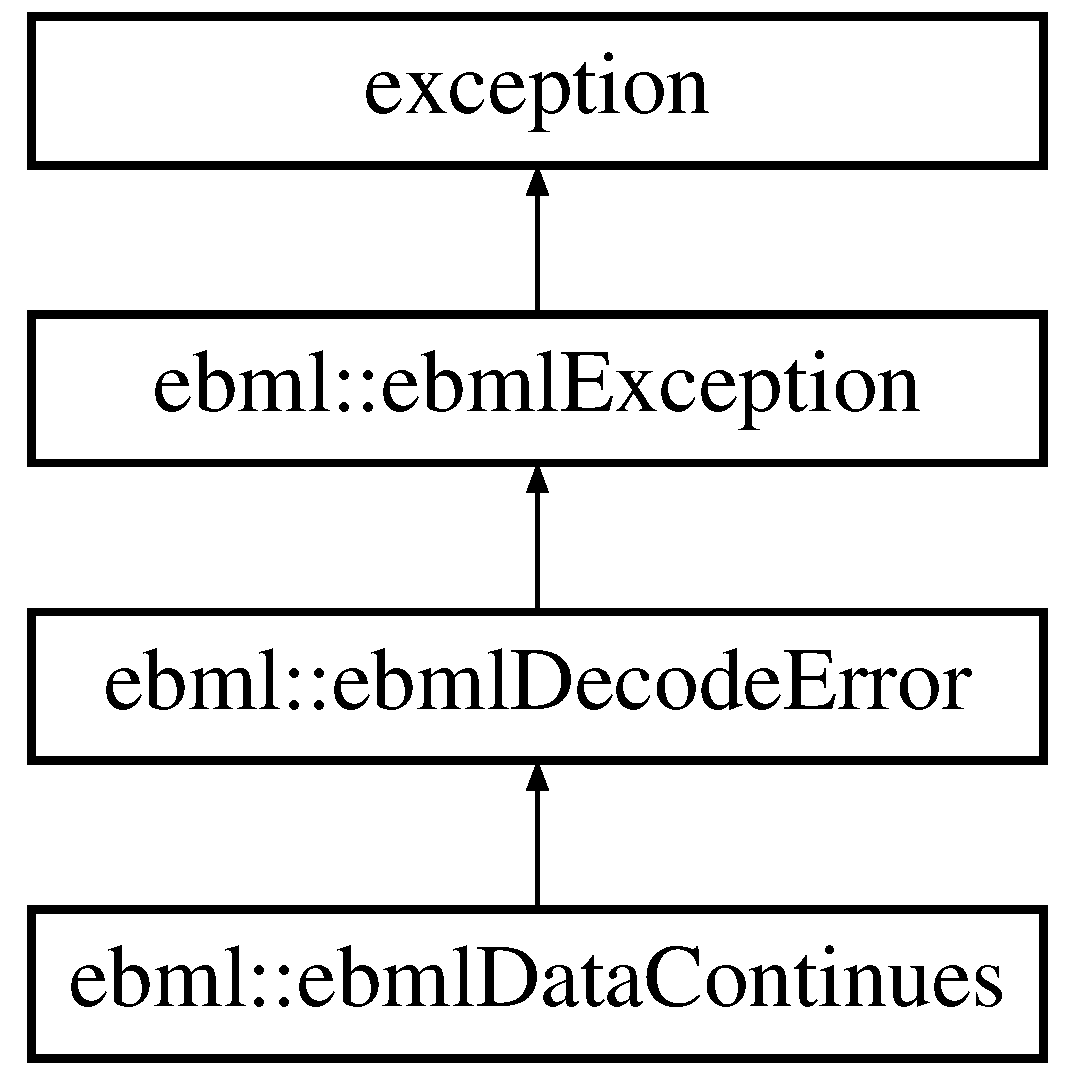
\includegraphics[height=4.000000cm]{classebml_1_1ebmlDataContinues}
\end{center}
\end{figure}
\subsection*{Public Member Functions}
\begin{DoxyCompactItemize}
\item 
\mbox{\hyperlink{classebml_1_1ebmlDataContinues_acc954c94b4650ccfa1513c5469e845c9}{ebml\+Data\+Continues}} (const std\+::string \&message, const \mbox{\hyperlink{classebml_1_1ebmlElementClass}{ebml\+Element\+Class}} $\ast$\mbox{\hyperlink{classebml_1_1ebmlDecodeError_a3568b4ea3cd5bd16b9510abfe269920f}{cls}}=nullptr, off\+\_\+t \mbox{\hyperlink{classebml_1_1ebmlDecodeError_ad32ac9b3dd52f1c11479085d9c665e0f}{offset}}=-\/1, unsigned char \mbox{\hyperlink{classebml_1_1ebmlDecodeError_a61a4d4856f0c779a1c216e45dc5a7c1e}{head\+Size}}=0, off\+\_\+t \mbox{\hyperlink{classebml_1_1ebmlDecodeError_acb525117e0109d9640fb5e8c546e9a02}{erroroffset}}=-\/1)
\end{DoxyCompactItemize}
\subsection*{Additional Inherited Members}


\subsection{Constructor \& Destructor Documentation}
\mbox{\Hypertarget{classebml_1_1ebmlDataContinues_acc954c94b4650ccfa1513c5469e845c9}\label{classebml_1_1ebmlDataContinues_acc954c94b4650ccfa1513c5469e845c9}} 
\index{ebml\+::ebml\+Data\+Continues@{ebml\+::ebml\+Data\+Continues}!ebml\+Data\+Continues@{ebml\+Data\+Continues}}
\index{ebml\+Data\+Continues@{ebml\+Data\+Continues}!ebml\+::ebml\+Data\+Continues@{ebml\+::ebml\+Data\+Continues}}
\subsubsection{\texorpdfstring{ebml\+Data\+Continues()}{ebmlDataContinues()}}
{\footnotesize\ttfamily ebml\+::ebml\+Data\+Continues\+::ebml\+Data\+Continues (\begin{DoxyParamCaption}\item[{const std\+::string \&}]{message,  }\item[{const \mbox{\hyperlink{classebml_1_1ebmlElementClass}{ebml\+Element\+Class}} $\ast$}]{cls = {\ttfamily nullptr},  }\item[{off\+\_\+t}]{offset = {\ttfamily -\/1},  }\item[{unsigned char}]{head\+Size = {\ttfamily 0},  }\item[{off\+\_\+t}]{erroroffset = {\ttfamily -\/1} }\end{DoxyParamCaption})}



The documentation for this class was generated from the following file\+:\begin{DoxyCompactItemize}
\item 
include/libebml\+\_\+ng/\mbox{\hyperlink{exceptions_8h}{exceptions.\+h}}\end{DoxyCompactItemize}

\hypertarget{classebml_1_1ebmlDataElement}{}\section{ebml\+:\+:ebml\+Data\+Element$<$ T $>$ Class Template Reference}
\label{classebml_1_1ebmlDataElement}\index{ebml\+::ebml\+Data\+Element$<$ T $>$@{ebml\+::ebml\+Data\+Element$<$ T $>$}}


{\ttfamily \#include $<$dataelement.\+h$>$}

Inheritance diagram for ebml\+:\+:ebml\+Data\+Element$<$ T $>$\+:\begin{figure}[H]
\begin{center}
\leavevmode
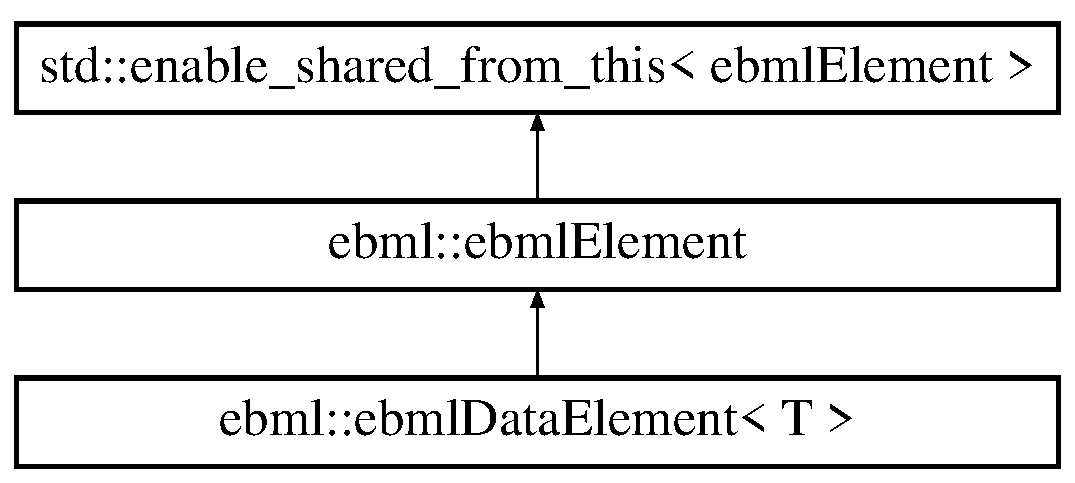
\includegraphics[height=3.000000cm]{classebml_1_1ebmlDataElement}
\end{center}
\end{figure}
\subsection*{Public Member Functions}
\begin{DoxyCompactItemize}
\item 
virtual size\+\_\+t \mbox{\hyperlink{classebml_1_1ebmlDataElement_add3cc3627008b8139a054a3a0696bc2d}{data\+Size}} () const
\item 
std\+::wstring \mbox{\hyperlink{classebml_1_1ebmlDataElement_a721eb3bfcb545510f2cebad65776f1bd}{minirepr}} () const
\end{DoxyCompactItemize}
\subsection*{Public Attributes}
\begin{DoxyCompactItemize}
\item 
T \mbox{\hyperlink{classebml_1_1ebmlDataElement_aa0b68d39cf69e0a34ba7bb1d8368a386}{data}}
\end{DoxyCompactItemize}
\subsection*{Protected Member Functions}
\begin{DoxyCompactItemize}
\item 
\mbox{\hyperlink{classebml_1_1ebmlDataElement_a9b130669c4ed313918eb8af37f067b1d}{ebml\+Data\+Element}} (const \mbox{\hyperlink{classebml_1_1ebmlDataElementClass}{ebml\+Data\+Element\+Class}}$<$ T $>$ $\ast$, const T \&)
\item 
\mbox{\hyperlink{classebml_1_1ebmlDataElement_a6006b80fd6faec7d0cc46a597c7073dc}{ebml\+Data\+Element}} (const \mbox{\hyperlink{classebml_1_1ebmlDataElementClass}{ebml\+Data\+Element\+Class}}$<$ T $>$ $\ast$, T \&\&)
\item 
virtual size\+\_\+t \mbox{\hyperlink{classebml_1_1ebmlDataElement_aabb10c15457709e0aa2c1f5744ddbfff}{\+\_\+encode}} (char $\ast$) const
\item 
virtual void \mbox{\hyperlink{classebml_1_1ebmlDataElement_abc9e99cdc566a08b2334e55374dc5f5a}{\+\_\+clonedata}} (const \mbox{\hyperlink{classebml_1_1ebmlElement}{ebml\+Element}} $\ast$)
\end{DoxyCompactItemize}
\subsection*{Friends}
\begin{DoxyCompactItemize}
\item 
class \mbox{\hyperlink{classebml_1_1ebmlDataElement_ae0bbbe5e14590a39747036bca3911c95}{ebml\+Data\+Element\+Class$<$ T $>$}}
\end{DoxyCompactItemize}
\subsection*{Additional Inherited Members}


\subsection{Constructor \& Destructor Documentation}
\mbox{\Hypertarget{classebml_1_1ebmlDataElement_a9b130669c4ed313918eb8af37f067b1d}\label{classebml_1_1ebmlDataElement_a9b130669c4ed313918eb8af37f067b1d}} 
\index{ebml\+::ebml\+Data\+Element@{ebml\+::ebml\+Data\+Element}!ebml\+Data\+Element@{ebml\+Data\+Element}}
\index{ebml\+Data\+Element@{ebml\+Data\+Element}!ebml\+::ebml\+Data\+Element@{ebml\+::ebml\+Data\+Element}}
\subsubsection{\texorpdfstring{ebml\+Data\+Element()}{ebmlDataElement()}\hspace{0.1cm}{\footnotesize\ttfamily [1/2]}}
{\footnotesize\ttfamily template$<$typename T $>$ \\
\mbox{\hyperlink{classebml_1_1ebmlDataElement}{ebml\+::ebml\+Data\+Element}}$<$ T $>$\+::\mbox{\hyperlink{classebml_1_1ebmlDataElement}{ebml\+Data\+Element}} (\begin{DoxyParamCaption}\item[{const \mbox{\hyperlink{classebml_1_1ebmlDataElementClass}{ebml\+Data\+Element\+Class}}$<$ T $>$ $\ast$}]{,  }\item[{const T \&}]{ }\end{DoxyParamCaption})\hspace{0.3cm}{\ttfamily [protected]}}

\mbox{\Hypertarget{classebml_1_1ebmlDataElement_a6006b80fd6faec7d0cc46a597c7073dc}\label{classebml_1_1ebmlDataElement_a6006b80fd6faec7d0cc46a597c7073dc}} 
\index{ebml\+::ebml\+Data\+Element@{ebml\+::ebml\+Data\+Element}!ebml\+Data\+Element@{ebml\+Data\+Element}}
\index{ebml\+Data\+Element@{ebml\+Data\+Element}!ebml\+::ebml\+Data\+Element@{ebml\+::ebml\+Data\+Element}}
\subsubsection{\texorpdfstring{ebml\+Data\+Element()}{ebmlDataElement()}\hspace{0.1cm}{\footnotesize\ttfamily [2/2]}}
{\footnotesize\ttfamily template$<$typename T $>$ \\
\mbox{\hyperlink{classebml_1_1ebmlDataElement}{ebml\+::ebml\+Data\+Element}}$<$ T $>$\+::\mbox{\hyperlink{classebml_1_1ebmlDataElement}{ebml\+Data\+Element}} (\begin{DoxyParamCaption}\item[{const \mbox{\hyperlink{classebml_1_1ebmlDataElementClass}{ebml\+Data\+Element\+Class}}$<$ T $>$ $\ast$}]{,  }\item[{T \&\&}]{ }\end{DoxyParamCaption})\hspace{0.3cm}{\ttfamily [protected]}}



\subsection{Member Function Documentation}
\mbox{\Hypertarget{classebml_1_1ebmlDataElement_abc9e99cdc566a08b2334e55374dc5f5a}\label{classebml_1_1ebmlDataElement_abc9e99cdc566a08b2334e55374dc5f5a}} 
\index{ebml\+::ebml\+Data\+Element@{ebml\+::ebml\+Data\+Element}!\+\_\+clonedata@{\+\_\+clonedata}}
\index{\+\_\+clonedata@{\+\_\+clonedata}!ebml\+::ebml\+Data\+Element@{ebml\+::ebml\+Data\+Element}}
\subsubsection{\texorpdfstring{\+\_\+clonedata()}{\_clonedata()}}
{\footnotesize\ttfamily template$<$typename T $>$ \\
virtual void \mbox{\hyperlink{classebml_1_1ebmlDataElement}{ebml\+::ebml\+Data\+Element}}$<$ T $>$\+::\+\_\+clonedata (\begin{DoxyParamCaption}\item[{const \mbox{\hyperlink{classebml_1_1ebmlElement}{ebml\+Element}} $\ast$}]{ }\end{DoxyParamCaption})\hspace{0.3cm}{\ttfamily [protected]}, {\ttfamily [virtual]}}



Implements \mbox{\hyperlink{classebml_1_1ebmlElement_a3ebe3aa75b62971f385c01f27c807a02}{ebml\+::ebml\+Element}}.

\mbox{\Hypertarget{classebml_1_1ebmlDataElement_aabb10c15457709e0aa2c1f5744ddbfff}\label{classebml_1_1ebmlDataElement_aabb10c15457709e0aa2c1f5744ddbfff}} 
\index{ebml\+::ebml\+Data\+Element@{ebml\+::ebml\+Data\+Element}!\+\_\+encode@{\+\_\+encode}}
\index{\+\_\+encode@{\+\_\+encode}!ebml\+::ebml\+Data\+Element@{ebml\+::ebml\+Data\+Element}}
\subsubsection{\texorpdfstring{\+\_\+encode()}{\_encode()}}
{\footnotesize\ttfamily template$<$typename T $>$ \\
virtual size\+\_\+t \mbox{\hyperlink{classebml_1_1ebmlDataElement}{ebml\+::ebml\+Data\+Element}}$<$ T $>$\+::\+\_\+encode (\begin{DoxyParamCaption}\item[{char $\ast$}]{ }\end{DoxyParamCaption}) const\hspace{0.3cm}{\ttfamily [protected]}, {\ttfamily [virtual]}}



Implements \mbox{\hyperlink{classebml_1_1ebmlElement_a27bd9de14e1706840235b68331917776}{ebml\+::ebml\+Element}}.

\mbox{\Hypertarget{classebml_1_1ebmlDataElement_add3cc3627008b8139a054a3a0696bc2d}\label{classebml_1_1ebmlDataElement_add3cc3627008b8139a054a3a0696bc2d}} 
\index{ebml\+::ebml\+Data\+Element@{ebml\+::ebml\+Data\+Element}!data\+Size@{data\+Size}}
\index{data\+Size@{data\+Size}!ebml\+::ebml\+Data\+Element@{ebml\+::ebml\+Data\+Element}}
\subsubsection{\texorpdfstring{data\+Size()}{dataSize()}}
{\footnotesize\ttfamily template$<$typename T $>$ \\
virtual size\+\_\+t \mbox{\hyperlink{classebml_1_1ebmlDataElement}{ebml\+::ebml\+Data\+Element}}$<$ T $>$\+::data\+Size (\begin{DoxyParamCaption}{ }\end{DoxyParamCaption}) const\hspace{0.3cm}{\ttfamily [virtual]}}



Implements \mbox{\hyperlink{classebml_1_1ebmlElement_a47ed4167d9c69104e02b6dbad0cd1fef}{ebml\+::ebml\+Element}}.

\mbox{\Hypertarget{classebml_1_1ebmlDataElement_a721eb3bfcb545510f2cebad65776f1bd}\label{classebml_1_1ebmlDataElement_a721eb3bfcb545510f2cebad65776f1bd}} 
\index{ebml\+::ebml\+Data\+Element@{ebml\+::ebml\+Data\+Element}!minirepr@{minirepr}}
\index{minirepr@{minirepr}!ebml\+::ebml\+Data\+Element@{ebml\+::ebml\+Data\+Element}}
\subsubsection{\texorpdfstring{minirepr()}{minirepr()}}
{\footnotesize\ttfamily template$<$typename T $>$ \\
std\+::wstring \mbox{\hyperlink{classebml_1_1ebmlDataElement}{ebml\+::ebml\+Data\+Element}}$<$ T $>$\+::minirepr (\begin{DoxyParamCaption}{ }\end{DoxyParamCaption}) const\hspace{0.3cm}{\ttfamily [virtual]}}



Implements \mbox{\hyperlink{classebml_1_1ebmlElement_a7852173aeef78bd843939ae5a82f1d1c}{ebml\+::ebml\+Element}}.



\subsection{Friends And Related Function Documentation}
\mbox{\Hypertarget{classebml_1_1ebmlDataElement_ae0bbbe5e14590a39747036bca3911c95}\label{classebml_1_1ebmlDataElement_ae0bbbe5e14590a39747036bca3911c95}} 
\index{ebml\+::ebml\+Data\+Element@{ebml\+::ebml\+Data\+Element}!ebml\+Data\+Element\+Class$<$ T $>$@{ebml\+Data\+Element\+Class$<$ T $>$}}
\index{ebml\+Data\+Element\+Class$<$ T $>$@{ebml\+Data\+Element\+Class$<$ T $>$}!ebml\+::ebml\+Data\+Element@{ebml\+::ebml\+Data\+Element}}
\subsubsection{\texorpdfstring{ebml\+Data\+Element\+Class$<$ T $>$}{ebmlDataElementClass< T >}}
{\footnotesize\ttfamily template$<$typename T $>$ \\
friend class \mbox{\hyperlink{classebml_1_1ebmlDataElementClass}{ebml\+Data\+Element\+Class}}$<$ T $>$\hspace{0.3cm}{\ttfamily [friend]}}



\subsection{Member Data Documentation}
\mbox{\Hypertarget{classebml_1_1ebmlDataElement_aa0b68d39cf69e0a34ba7bb1d8368a386}\label{classebml_1_1ebmlDataElement_aa0b68d39cf69e0a34ba7bb1d8368a386}} 
\index{ebml\+::ebml\+Data\+Element@{ebml\+::ebml\+Data\+Element}!data@{data}}
\index{data@{data}!ebml\+::ebml\+Data\+Element@{ebml\+::ebml\+Data\+Element}}
\subsubsection{\texorpdfstring{data}{data}}
{\footnotesize\ttfamily template$<$typename T $>$ \\
T \mbox{\hyperlink{classebml_1_1ebmlDataElement}{ebml\+::ebml\+Data\+Element}}$<$ T $>$\+::data}



The documentation for this class was generated from the following file\+:\begin{DoxyCompactItemize}
\item 
include/libebml\+\_\+ng/\mbox{\hyperlink{dataelement_8h}{dataelement.\+h}}\end{DoxyCompactItemize}

\hypertarget{classebml_1_1ebmlDataElement_3_01const_01T_01_4}{}\section{ebml\+:\+:ebml\+Data\+Element$<$ const T $>$ Class Template Reference}
\label{classebml_1_1ebmlDataElement_3_01const_01T_01_4}\index{ebml\+::ebml\+Data\+Element$<$ const T $>$@{ebml\+::ebml\+Data\+Element$<$ const T $>$}}


{\ttfamily \#include $<$dataelement.\+h$>$}

Inheritance diagram for ebml\+:\+:ebml\+Data\+Element$<$ const T $>$\+:\begin{figure}[H]
\begin{center}
\leavevmode
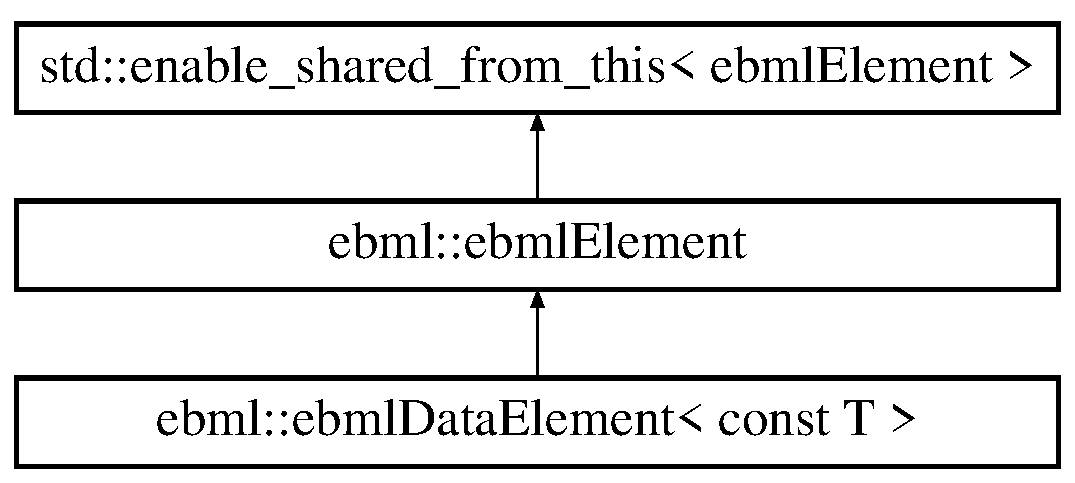
\includegraphics[height=3.000000cm]{classebml_1_1ebmlDataElement_3_01const_01T_01_4}
\end{center}
\end{figure}
\subsection*{Public Member Functions}
\begin{DoxyCompactItemize}
\item 
const \mbox{\hyperlink{classebml_1_1ebmlDataElementClass}{ebml\+Data\+Element\+Class}}$<$ const T $>$ $\ast$ \mbox{\hyperlink{classebml_1_1ebmlDataElement_3_01const_01T_01_4_a27173a9d7784ce0cfca71e1c72c36ec7}{cls}} () const
\item 
virtual size\+\_\+t \mbox{\hyperlink{classebml_1_1ebmlDataElement_3_01const_01T_01_4_a0965d2da67f1862d2c806151063dcfce}{data\+Size}} () const
\item 
\mbox{\hyperlink{namespaceebml_adad533b7705a16bb360fe56380c5e7be}{ebml\+Element\+\_\+sp}} \mbox{\hyperlink{classebml_1_1ebmlDataElement_3_01const_01T_01_4_a23f7032682dfdf20ce042caf144e50d6}{clone}} () const
\item 
std\+::wstring \mbox{\hyperlink{classebml_1_1ebmlDataElement_3_01const_01T_01_4_aa5a82c4528609bf788caf8db8927fbc1}{minirepr}} () const
\end{DoxyCompactItemize}
\subsection*{Public Attributes}
\begin{DoxyCompactItemize}
\item 
T \mbox{\hyperlink{classebml_1_1ebmlDataElement_3_01const_01T_01_4_ac3870bb3b5d9d0e3063a80768fe83904}{data}}
\end{DoxyCompactItemize}
\subsection*{Protected Member Functions}
\begin{DoxyCompactItemize}
\item 
\mbox{\hyperlink{classebml_1_1ebmlDataElement_3_01const_01T_01_4_abb559dd529796adda5e2ea9b8bedf876}{ebml\+Data\+Element}} (const \mbox{\hyperlink{classebml_1_1ebmlDataElementClass}{ebml\+Data\+Element\+Class}}$<$ const T $>$ $\ast$, const T \&)
\item 
\mbox{\hyperlink{classebml_1_1ebmlDataElement_3_01const_01T_01_4_aafdd5fd8f53e58c34891419df8fd196f}{ebml\+Data\+Element}} (const \mbox{\hyperlink{classebml_1_1ebmlDataElementClass}{ebml\+Data\+Element\+Class}}$<$ const T $>$ $\ast$, T \&\&)
\item 
virtual size\+\_\+t \mbox{\hyperlink{classebml_1_1ebmlDataElement_3_01const_01T_01_4_aac802a573eaeaa5b856d5e74deb9dd3a}{\+\_\+encode}} (char $\ast$) const
\item 
void \mbox{\hyperlink{classebml_1_1ebmlDataElement_3_01const_01T_01_4_a46a152b21a6fc49a331e61f29c486ebe}{\+\_\+clonedata}} (const \mbox{\hyperlink{classebml_1_1ebmlElement}{ebml\+Element}} $\ast$)
\end{DoxyCompactItemize}
\subsection*{Friends}
\begin{DoxyCompactItemize}
\item 
class \mbox{\hyperlink{classebml_1_1ebmlDataElement_3_01const_01T_01_4_aea1d7162edf00e39cf37b106860abbcd}{ebml\+Data\+Element\+Class$<$ const T $>$}}
\end{DoxyCompactItemize}
\subsection*{Additional Inherited Members}


\subsection{Constructor \& Destructor Documentation}
\mbox{\Hypertarget{classebml_1_1ebmlDataElement_3_01const_01T_01_4_abb559dd529796adda5e2ea9b8bedf876}\label{classebml_1_1ebmlDataElement_3_01const_01T_01_4_abb559dd529796adda5e2ea9b8bedf876}} 
\index{ebml\+::ebml\+Data\+Element$<$ const T $>$@{ebml\+::ebml\+Data\+Element$<$ const T $>$}!ebml\+Data\+Element@{ebml\+Data\+Element}}
\index{ebml\+Data\+Element@{ebml\+Data\+Element}!ebml\+::ebml\+Data\+Element$<$ const T $>$@{ebml\+::ebml\+Data\+Element$<$ const T $>$}}
\subsubsection{\texorpdfstring{ebml\+Data\+Element()}{ebmlDataElement()}\hspace{0.1cm}{\footnotesize\ttfamily [1/2]}}
{\footnotesize\ttfamily template$<$typename T $>$ \\
\mbox{\hyperlink{classebml_1_1ebmlDataElement}{ebml\+::ebml\+Data\+Element}}$<$ const T $>$\+::\mbox{\hyperlink{classebml_1_1ebmlDataElement}{ebml\+Data\+Element}} (\begin{DoxyParamCaption}\item[{const \mbox{\hyperlink{classebml_1_1ebmlDataElementClass}{ebml\+Data\+Element\+Class}}$<$ const T $>$ $\ast$}]{,  }\item[{const T \&}]{ }\end{DoxyParamCaption})\hspace{0.3cm}{\ttfamily [protected]}}

\mbox{\Hypertarget{classebml_1_1ebmlDataElement_3_01const_01T_01_4_aafdd5fd8f53e58c34891419df8fd196f}\label{classebml_1_1ebmlDataElement_3_01const_01T_01_4_aafdd5fd8f53e58c34891419df8fd196f}} 
\index{ebml\+::ebml\+Data\+Element$<$ const T $>$@{ebml\+::ebml\+Data\+Element$<$ const T $>$}!ebml\+Data\+Element@{ebml\+Data\+Element}}
\index{ebml\+Data\+Element@{ebml\+Data\+Element}!ebml\+::ebml\+Data\+Element$<$ const T $>$@{ebml\+::ebml\+Data\+Element$<$ const T $>$}}
\subsubsection{\texorpdfstring{ebml\+Data\+Element()}{ebmlDataElement()}\hspace{0.1cm}{\footnotesize\ttfamily [2/2]}}
{\footnotesize\ttfamily template$<$typename T $>$ \\
\mbox{\hyperlink{classebml_1_1ebmlDataElement}{ebml\+::ebml\+Data\+Element}}$<$ const T $>$\+::\mbox{\hyperlink{classebml_1_1ebmlDataElement}{ebml\+Data\+Element}} (\begin{DoxyParamCaption}\item[{const \mbox{\hyperlink{classebml_1_1ebmlDataElementClass}{ebml\+Data\+Element\+Class}}$<$ const T $>$ $\ast$}]{,  }\item[{T \&\&}]{ }\end{DoxyParamCaption})\hspace{0.3cm}{\ttfamily [protected]}}



\subsection{Member Function Documentation}
\mbox{\Hypertarget{classebml_1_1ebmlDataElement_3_01const_01T_01_4_a46a152b21a6fc49a331e61f29c486ebe}\label{classebml_1_1ebmlDataElement_3_01const_01T_01_4_a46a152b21a6fc49a331e61f29c486ebe}} 
\index{ebml\+::ebml\+Data\+Element$<$ const T $>$@{ebml\+::ebml\+Data\+Element$<$ const T $>$}!\+\_\+clonedata@{\+\_\+clonedata}}
\index{\+\_\+clonedata@{\+\_\+clonedata}!ebml\+::ebml\+Data\+Element$<$ const T $>$@{ebml\+::ebml\+Data\+Element$<$ const T $>$}}
\subsubsection{\texorpdfstring{\+\_\+clonedata()}{\_clonedata()}}
{\footnotesize\ttfamily template$<$typename T $>$ \\
void \mbox{\hyperlink{classebml_1_1ebmlDataElement}{ebml\+::ebml\+Data\+Element}}$<$ const T $>$\+::\+\_\+clonedata (\begin{DoxyParamCaption}\item[{const \mbox{\hyperlink{classebml_1_1ebmlElement}{ebml\+Element}} $\ast$}]{ }\end{DoxyParamCaption})\hspace{0.3cm}{\ttfamily [protected]}, {\ttfamily [virtual]}}



Implements \mbox{\hyperlink{classebml_1_1ebmlElement_a3ebe3aa75b62971f385c01f27c807a02}{ebml\+::ebml\+Element}}.

\mbox{\Hypertarget{classebml_1_1ebmlDataElement_3_01const_01T_01_4_aac802a573eaeaa5b856d5e74deb9dd3a}\label{classebml_1_1ebmlDataElement_3_01const_01T_01_4_aac802a573eaeaa5b856d5e74deb9dd3a}} 
\index{ebml\+::ebml\+Data\+Element$<$ const T $>$@{ebml\+::ebml\+Data\+Element$<$ const T $>$}!\+\_\+encode@{\+\_\+encode}}
\index{\+\_\+encode@{\+\_\+encode}!ebml\+::ebml\+Data\+Element$<$ const T $>$@{ebml\+::ebml\+Data\+Element$<$ const T $>$}}
\subsubsection{\texorpdfstring{\+\_\+encode()}{\_encode()}}
{\footnotesize\ttfamily template$<$typename T $>$ \\
virtual size\+\_\+t \mbox{\hyperlink{classebml_1_1ebmlDataElement}{ebml\+::ebml\+Data\+Element}}$<$ const T $>$\+::\+\_\+encode (\begin{DoxyParamCaption}\item[{char $\ast$}]{ }\end{DoxyParamCaption}) const\hspace{0.3cm}{\ttfamily [protected]}, {\ttfamily [virtual]}}



Implements \mbox{\hyperlink{classebml_1_1ebmlElement_a27bd9de14e1706840235b68331917776}{ebml\+::ebml\+Element}}.

\mbox{\Hypertarget{classebml_1_1ebmlDataElement_3_01const_01T_01_4_a23f7032682dfdf20ce042caf144e50d6}\label{classebml_1_1ebmlDataElement_3_01const_01T_01_4_a23f7032682dfdf20ce042caf144e50d6}} 
\index{ebml\+::ebml\+Data\+Element$<$ const T $>$@{ebml\+::ebml\+Data\+Element$<$ const T $>$}!clone@{clone}}
\index{clone@{clone}!ebml\+::ebml\+Data\+Element$<$ const T $>$@{ebml\+::ebml\+Data\+Element$<$ const T $>$}}
\subsubsection{\texorpdfstring{clone()}{clone()}}
{\footnotesize\ttfamily template$<$typename T $>$ \\
\mbox{\hyperlink{namespaceebml_adad533b7705a16bb360fe56380c5e7be}{ebml\+Element\+\_\+sp}} \mbox{\hyperlink{classebml_1_1ebmlDataElement}{ebml\+::ebml\+Data\+Element}}$<$ const T $>$\+::clone (\begin{DoxyParamCaption}{ }\end{DoxyParamCaption}) const\hspace{0.3cm}{\ttfamily [virtual]}}



Reimplemented from \mbox{\hyperlink{classebml_1_1ebmlElement_a94013f01b6f12c9c66864d44983dce47}{ebml\+::ebml\+Element}}.

\mbox{\Hypertarget{classebml_1_1ebmlDataElement_3_01const_01T_01_4_a27173a9d7784ce0cfca71e1c72c36ec7}\label{classebml_1_1ebmlDataElement_3_01const_01T_01_4_a27173a9d7784ce0cfca71e1c72c36ec7}} 
\index{ebml\+::ebml\+Data\+Element$<$ const T $>$@{ebml\+::ebml\+Data\+Element$<$ const T $>$}!cls@{cls}}
\index{cls@{cls}!ebml\+::ebml\+Data\+Element$<$ const T $>$@{ebml\+::ebml\+Data\+Element$<$ const T $>$}}
\subsubsection{\texorpdfstring{cls()}{cls()}}
{\footnotesize\ttfamily template$<$typename T $>$ \\
const \mbox{\hyperlink{classebml_1_1ebmlDataElementClass}{ebml\+Data\+Element\+Class}}$<$const T$>$$\ast$ \mbox{\hyperlink{classebml_1_1ebmlDataElement}{ebml\+::ebml\+Data\+Element}}$<$ const T $>$\+::cls (\begin{DoxyParamCaption}{ }\end{DoxyParamCaption}) const\hspace{0.3cm}{\ttfamily [virtual]}}



Reimplemented from \mbox{\hyperlink{classebml_1_1ebmlElement_a15cf59e94b01e2c49ec96512b9bd9d90}{ebml\+::ebml\+Element}}.

\mbox{\Hypertarget{classebml_1_1ebmlDataElement_3_01const_01T_01_4_a0965d2da67f1862d2c806151063dcfce}\label{classebml_1_1ebmlDataElement_3_01const_01T_01_4_a0965d2da67f1862d2c806151063dcfce}} 
\index{ebml\+::ebml\+Data\+Element$<$ const T $>$@{ebml\+::ebml\+Data\+Element$<$ const T $>$}!data\+Size@{data\+Size}}
\index{data\+Size@{data\+Size}!ebml\+::ebml\+Data\+Element$<$ const T $>$@{ebml\+::ebml\+Data\+Element$<$ const T $>$}}
\subsubsection{\texorpdfstring{data\+Size()}{dataSize()}}
{\footnotesize\ttfamily template$<$typename T $>$ \\
virtual size\+\_\+t \mbox{\hyperlink{classebml_1_1ebmlDataElement}{ebml\+::ebml\+Data\+Element}}$<$ const T $>$\+::data\+Size (\begin{DoxyParamCaption}{ }\end{DoxyParamCaption}) const\hspace{0.3cm}{\ttfamily [virtual]}}



Implements \mbox{\hyperlink{classebml_1_1ebmlElement_a47ed4167d9c69104e02b6dbad0cd1fef}{ebml\+::ebml\+Element}}.

\mbox{\Hypertarget{classebml_1_1ebmlDataElement_3_01const_01T_01_4_aa5a82c4528609bf788caf8db8927fbc1}\label{classebml_1_1ebmlDataElement_3_01const_01T_01_4_aa5a82c4528609bf788caf8db8927fbc1}} 
\index{ebml\+::ebml\+Data\+Element$<$ const T $>$@{ebml\+::ebml\+Data\+Element$<$ const T $>$}!minirepr@{minirepr}}
\index{minirepr@{minirepr}!ebml\+::ebml\+Data\+Element$<$ const T $>$@{ebml\+::ebml\+Data\+Element$<$ const T $>$}}
\subsubsection{\texorpdfstring{minirepr()}{minirepr()}}
{\footnotesize\ttfamily template$<$typename T $>$ \\
std\+::wstring \mbox{\hyperlink{classebml_1_1ebmlDataElement}{ebml\+::ebml\+Data\+Element}}$<$ const T $>$\+::minirepr (\begin{DoxyParamCaption}{ }\end{DoxyParamCaption}) const\hspace{0.3cm}{\ttfamily [virtual]}}



Implements \mbox{\hyperlink{classebml_1_1ebmlElement_a7852173aeef78bd843939ae5a82f1d1c}{ebml\+::ebml\+Element}}.



\subsection{Friends And Related Function Documentation}
\mbox{\Hypertarget{classebml_1_1ebmlDataElement_3_01const_01T_01_4_aea1d7162edf00e39cf37b106860abbcd}\label{classebml_1_1ebmlDataElement_3_01const_01T_01_4_aea1d7162edf00e39cf37b106860abbcd}} 
\index{ebml\+::ebml\+Data\+Element$<$ const T $>$@{ebml\+::ebml\+Data\+Element$<$ const T $>$}!ebml\+Data\+Element\+Class$<$ const T $>$@{ebml\+Data\+Element\+Class$<$ const T $>$}}
\index{ebml\+Data\+Element\+Class$<$ const T $>$@{ebml\+Data\+Element\+Class$<$ const T $>$}!ebml\+::ebml\+Data\+Element$<$ const T $>$@{ebml\+::ebml\+Data\+Element$<$ const T $>$}}
\subsubsection{\texorpdfstring{ebml\+Data\+Element\+Class$<$ const T $>$}{ebmlDataElementClass< const T >}}
{\footnotesize\ttfamily template$<$typename T $>$ \\
friend class \mbox{\hyperlink{classebml_1_1ebmlDataElementClass}{ebml\+Data\+Element\+Class}}$<$ const T $>$\hspace{0.3cm}{\ttfamily [friend]}}



\subsection{Member Data Documentation}
\mbox{\Hypertarget{classebml_1_1ebmlDataElement_3_01const_01T_01_4_ac3870bb3b5d9d0e3063a80768fe83904}\label{classebml_1_1ebmlDataElement_3_01const_01T_01_4_ac3870bb3b5d9d0e3063a80768fe83904}} 
\index{ebml\+::ebml\+Data\+Element$<$ const T $>$@{ebml\+::ebml\+Data\+Element$<$ const T $>$}!data@{data}}
\index{data@{data}!ebml\+::ebml\+Data\+Element$<$ const T $>$@{ebml\+::ebml\+Data\+Element$<$ const T $>$}}
\subsubsection{\texorpdfstring{data}{data}}
{\footnotesize\ttfamily template$<$typename T $>$ \\
T \mbox{\hyperlink{classebml_1_1ebmlDataElement}{ebml\+::ebml\+Data\+Element}}$<$ const T $>$\+::data}



The documentation for this class was generated from the following file\+:\begin{DoxyCompactItemize}
\item 
include/libebml\+\_\+ng/\mbox{\hyperlink{dataelement_8h}{dataelement.\+h}}\end{DoxyCompactItemize}

\hypertarget{classebml_1_1ebmlDataElementClass}{}\section{ebml\+:\+:ebml\+Data\+Element\+Class$<$ T $>$ Class Template Reference}
\label{classebml_1_1ebmlDataElementClass}\index{ebml\+::ebml\+Data\+Element\+Class$<$ T $>$@{ebml\+::ebml\+Data\+Element\+Class$<$ T $>$}}


{\ttfamily \#include $<$template.\+h$>$}

Inheritance diagram for ebml\+:\+:ebml\+Data\+Element\+Class$<$ T $>$\+:\begin{figure}[H]
\begin{center}
\leavevmode
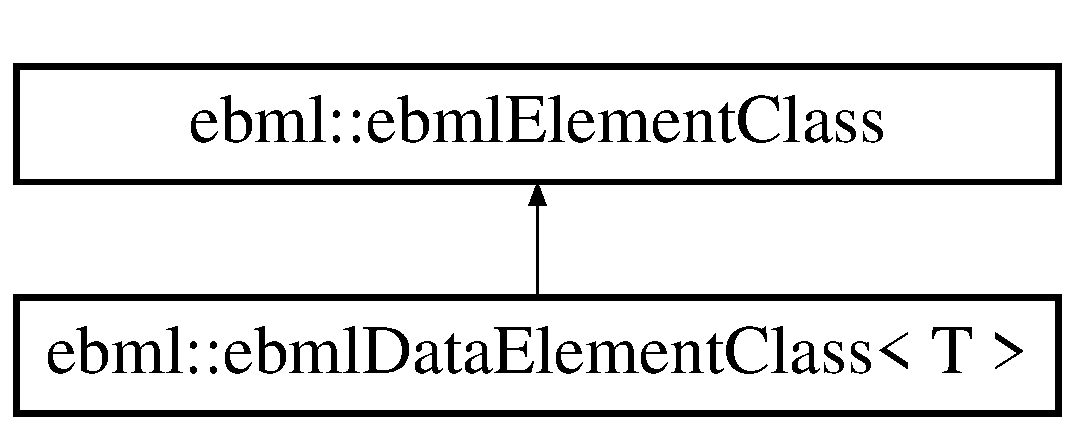
\includegraphics[height=2.000000cm]{classebml_1_1ebmlDataElementClass}
\end{center}
\end{figure}
\subsection*{Public Member Functions}
\begin{DoxyCompactItemize}
\item 
\mbox{\hyperlink{classebml_1_1ebmlDataElementClass_a9fc67c00537acbd8c4e67c62d4e8a877}{ebml\+Data\+Element\+Class}} (const char $\ast$, const std\+::wstring \&)
\item 
\mbox{\hyperlink{classebml_1_1ebmlDataElementClass_a9041c4768574aa8a05008622c59d1505}{ebml\+Data\+Element\+Class}} (const char $\ast$, const std\+::wstring \&, const T \&)
\item 
\mbox{\hyperlink{classebml_1_1ebmlDataElementClass_a563cc43ab0bffe8be47cd3c675ce675e}{ebml\+Data\+Element\+Class}} (const char $\ast$, const std\+::wstring \&, T \&\&)
\item 
\mbox{\hyperlink{classebml_1_1ebmlDataElementClass_a96c16b441ed04a1c34ff2f52d6a86655}{ebml\+Data\+Element\+Class}} (\mbox{\hyperlink{namespaceebml_a86c5f604ddf12a74aa9812e997a58691}{ebml\+I\+D\+\_\+t}}, const std\+::wstring \&)
\item 
\mbox{\hyperlink{classebml_1_1ebmlDataElementClass_a7b0726f332f9abadac8b7b4672cf1013}{ebml\+Data\+Element\+Class}} (\mbox{\hyperlink{namespaceebml_a86c5f604ddf12a74aa9812e997a58691}{ebml\+I\+D\+\_\+t}}, const std\+::wstring \&, const T \&)
\item 
\mbox{\hyperlink{classebml_1_1ebmlDataElementClass_a3af7912dc41d400db7b1347766fef924}{ebml\+Data\+Element\+Class}} (\mbox{\hyperlink{namespaceebml_a86c5f604ddf12a74aa9812e997a58691}{ebml\+I\+D\+\_\+t}}, const std\+::wstring \&, T \&\&)
\item 
virtual \mbox{\hyperlink{namespaceebml_adad533b7705a16bb360fe56380c5e7be}{ebml\+Element\+\_\+sp}} \mbox{\hyperlink{classebml_1_1ebmlDataElementClass_af50d05f41174fbac6efa1a8cbdc5b4fe}{operator()}} (const T \&) const
\item 
virtual \mbox{\hyperlink{namespaceebml_adad533b7705a16bb360fe56380c5e7be}{ebml\+Element\+\_\+sp}} \mbox{\hyperlink{classebml_1_1ebmlDataElementClass_a4e5efa44d8b7440b16bb3df7754c4544}{operator()}} (T \&\&) const
\end{DoxyCompactItemize}
\subsection*{Public Attributes}
\begin{DoxyCompactItemize}
\item 
T \mbox{\hyperlink{classebml_1_1ebmlDataElementClass_a5ad1fcb2708f62d3d80eab6d9ad112be}{defaultval}}
\end{DoxyCompactItemize}
\subsection*{Static Public Attributes}
\begin{DoxyCompactItemize}
\item 
static T \mbox{\hyperlink{classebml_1_1ebmlDataElementClass_aa58b82cbc57d5ba83c54e845cf354bb5}{defaultdefault}}
\end{DoxyCompactItemize}
\subsection*{Protected Member Functions}
\begin{DoxyCompactItemize}
\item 
\mbox{\hyperlink{classebml_1_1ebmlElement}{ebml\+Element}} $\ast$ \mbox{\hyperlink{classebml_1_1ebmlDataElementClass_a022ddc37a9bf678de66dab9157d08b9a}{\+\_\+new}} () const
\end{DoxyCompactItemize}
\subsection*{Friends}
\begin{DoxyCompactItemize}
\item 
class \mbox{\hyperlink{classebml_1_1ebmlDataElementClass_a817c43c32db8e0094e44cb83006f25ca}{ebml\+Data\+Element$<$ T $>$}}
\end{DoxyCompactItemize}


\subsection{Constructor \& Destructor Documentation}
\mbox{\Hypertarget{classebml_1_1ebmlDataElementClass_a9fc67c00537acbd8c4e67c62d4e8a877}\label{classebml_1_1ebmlDataElementClass_a9fc67c00537acbd8c4e67c62d4e8a877}} 
\index{ebml\+::ebml\+Data\+Element\+Class@{ebml\+::ebml\+Data\+Element\+Class}!ebml\+Data\+Element\+Class@{ebml\+Data\+Element\+Class}}
\index{ebml\+Data\+Element\+Class@{ebml\+Data\+Element\+Class}!ebml\+::ebml\+Data\+Element\+Class@{ebml\+::ebml\+Data\+Element\+Class}}
\subsubsection{\texorpdfstring{ebml\+Data\+Element\+Class()}{ebmlDataElementClass()}\hspace{0.1cm}{\footnotesize\ttfamily [1/6]}}
{\footnotesize\ttfamily template$<$typename T$>$ \\
\mbox{\hyperlink{classebml_1_1ebmlDataElementClass}{ebml\+::ebml\+Data\+Element\+Class}}$<$ T $>$\+::\mbox{\hyperlink{classebml_1_1ebmlDataElementClass}{ebml\+Data\+Element\+Class}} (\begin{DoxyParamCaption}\item[{const char $\ast$}]{,  }\item[{const std\+::wstring \&}]{ }\end{DoxyParamCaption})}

\mbox{\Hypertarget{classebml_1_1ebmlDataElementClass_a9041c4768574aa8a05008622c59d1505}\label{classebml_1_1ebmlDataElementClass_a9041c4768574aa8a05008622c59d1505}} 
\index{ebml\+::ebml\+Data\+Element\+Class@{ebml\+::ebml\+Data\+Element\+Class}!ebml\+Data\+Element\+Class@{ebml\+Data\+Element\+Class}}
\index{ebml\+Data\+Element\+Class@{ebml\+Data\+Element\+Class}!ebml\+::ebml\+Data\+Element\+Class@{ebml\+::ebml\+Data\+Element\+Class}}
\subsubsection{\texorpdfstring{ebml\+Data\+Element\+Class()}{ebmlDataElementClass()}\hspace{0.1cm}{\footnotesize\ttfamily [2/6]}}
{\footnotesize\ttfamily template$<$typename T$>$ \\
\mbox{\hyperlink{classebml_1_1ebmlDataElementClass}{ebml\+::ebml\+Data\+Element\+Class}}$<$ T $>$\+::\mbox{\hyperlink{classebml_1_1ebmlDataElementClass}{ebml\+Data\+Element\+Class}} (\begin{DoxyParamCaption}\item[{const char $\ast$}]{,  }\item[{const std\+::wstring \&}]{,  }\item[{const T \&}]{ }\end{DoxyParamCaption})}

\mbox{\Hypertarget{classebml_1_1ebmlDataElementClass_a563cc43ab0bffe8be47cd3c675ce675e}\label{classebml_1_1ebmlDataElementClass_a563cc43ab0bffe8be47cd3c675ce675e}} 
\index{ebml\+::ebml\+Data\+Element\+Class@{ebml\+::ebml\+Data\+Element\+Class}!ebml\+Data\+Element\+Class@{ebml\+Data\+Element\+Class}}
\index{ebml\+Data\+Element\+Class@{ebml\+Data\+Element\+Class}!ebml\+::ebml\+Data\+Element\+Class@{ebml\+::ebml\+Data\+Element\+Class}}
\subsubsection{\texorpdfstring{ebml\+Data\+Element\+Class()}{ebmlDataElementClass()}\hspace{0.1cm}{\footnotesize\ttfamily [3/6]}}
{\footnotesize\ttfamily template$<$typename T$>$ \\
\mbox{\hyperlink{classebml_1_1ebmlDataElementClass}{ebml\+::ebml\+Data\+Element\+Class}}$<$ T $>$\+::\mbox{\hyperlink{classebml_1_1ebmlDataElementClass}{ebml\+Data\+Element\+Class}} (\begin{DoxyParamCaption}\item[{const char $\ast$}]{,  }\item[{const std\+::wstring \&}]{,  }\item[{T \&\&}]{ }\end{DoxyParamCaption})}

\mbox{\Hypertarget{classebml_1_1ebmlDataElementClass_a96c16b441ed04a1c34ff2f52d6a86655}\label{classebml_1_1ebmlDataElementClass_a96c16b441ed04a1c34ff2f52d6a86655}} 
\index{ebml\+::ebml\+Data\+Element\+Class@{ebml\+::ebml\+Data\+Element\+Class}!ebml\+Data\+Element\+Class@{ebml\+Data\+Element\+Class}}
\index{ebml\+Data\+Element\+Class@{ebml\+Data\+Element\+Class}!ebml\+::ebml\+Data\+Element\+Class@{ebml\+::ebml\+Data\+Element\+Class}}
\subsubsection{\texorpdfstring{ebml\+Data\+Element\+Class()}{ebmlDataElementClass()}\hspace{0.1cm}{\footnotesize\ttfamily [4/6]}}
{\footnotesize\ttfamily template$<$typename T$>$ \\
\mbox{\hyperlink{classebml_1_1ebmlDataElementClass}{ebml\+::ebml\+Data\+Element\+Class}}$<$ T $>$\+::\mbox{\hyperlink{classebml_1_1ebmlDataElementClass}{ebml\+Data\+Element\+Class}} (\begin{DoxyParamCaption}\item[{\mbox{\hyperlink{namespaceebml_a86c5f604ddf12a74aa9812e997a58691}{ebml\+I\+D\+\_\+t}}}]{,  }\item[{const std\+::wstring \&}]{ }\end{DoxyParamCaption})}

\mbox{\Hypertarget{classebml_1_1ebmlDataElementClass_a7b0726f332f9abadac8b7b4672cf1013}\label{classebml_1_1ebmlDataElementClass_a7b0726f332f9abadac8b7b4672cf1013}} 
\index{ebml\+::ebml\+Data\+Element\+Class@{ebml\+::ebml\+Data\+Element\+Class}!ebml\+Data\+Element\+Class@{ebml\+Data\+Element\+Class}}
\index{ebml\+Data\+Element\+Class@{ebml\+Data\+Element\+Class}!ebml\+::ebml\+Data\+Element\+Class@{ebml\+::ebml\+Data\+Element\+Class}}
\subsubsection{\texorpdfstring{ebml\+Data\+Element\+Class()}{ebmlDataElementClass()}\hspace{0.1cm}{\footnotesize\ttfamily [5/6]}}
{\footnotesize\ttfamily template$<$typename T$>$ \\
\mbox{\hyperlink{classebml_1_1ebmlDataElementClass}{ebml\+::ebml\+Data\+Element\+Class}}$<$ T $>$\+::\mbox{\hyperlink{classebml_1_1ebmlDataElementClass}{ebml\+Data\+Element\+Class}} (\begin{DoxyParamCaption}\item[{\mbox{\hyperlink{namespaceebml_a86c5f604ddf12a74aa9812e997a58691}{ebml\+I\+D\+\_\+t}}}]{,  }\item[{const std\+::wstring \&}]{,  }\item[{const T \&}]{ }\end{DoxyParamCaption})}

\mbox{\Hypertarget{classebml_1_1ebmlDataElementClass_a3af7912dc41d400db7b1347766fef924}\label{classebml_1_1ebmlDataElementClass_a3af7912dc41d400db7b1347766fef924}} 
\index{ebml\+::ebml\+Data\+Element\+Class@{ebml\+::ebml\+Data\+Element\+Class}!ebml\+Data\+Element\+Class@{ebml\+Data\+Element\+Class}}
\index{ebml\+Data\+Element\+Class@{ebml\+Data\+Element\+Class}!ebml\+::ebml\+Data\+Element\+Class@{ebml\+::ebml\+Data\+Element\+Class}}
\subsubsection{\texorpdfstring{ebml\+Data\+Element\+Class()}{ebmlDataElementClass()}\hspace{0.1cm}{\footnotesize\ttfamily [6/6]}}
{\footnotesize\ttfamily template$<$typename T$>$ \\
\mbox{\hyperlink{classebml_1_1ebmlDataElementClass}{ebml\+::ebml\+Data\+Element\+Class}}$<$ T $>$\+::\mbox{\hyperlink{classebml_1_1ebmlDataElementClass}{ebml\+Data\+Element\+Class}} (\begin{DoxyParamCaption}\item[{\mbox{\hyperlink{namespaceebml_a86c5f604ddf12a74aa9812e997a58691}{ebml\+I\+D\+\_\+t}}}]{,  }\item[{const std\+::wstring \&}]{,  }\item[{T \&\&}]{ }\end{DoxyParamCaption})}



\subsection{Member Function Documentation}
\mbox{\Hypertarget{classebml_1_1ebmlDataElementClass_a022ddc37a9bf678de66dab9157d08b9a}\label{classebml_1_1ebmlDataElementClass_a022ddc37a9bf678de66dab9157d08b9a}} 
\index{ebml\+::ebml\+Data\+Element\+Class@{ebml\+::ebml\+Data\+Element\+Class}!\+\_\+new@{\+\_\+new}}
\index{\+\_\+new@{\+\_\+new}!ebml\+::ebml\+Data\+Element\+Class@{ebml\+::ebml\+Data\+Element\+Class}}
\subsubsection{\texorpdfstring{\+\_\+new()}{\_new()}}
{\footnotesize\ttfamily template$<$typename T$>$ \\
\mbox{\hyperlink{classebml_1_1ebmlElement}{ebml\+Element}}$\ast$ \mbox{\hyperlink{classebml_1_1ebmlDataElementClass}{ebml\+::ebml\+Data\+Element\+Class}}$<$ T $>$\+::\+\_\+new (\begin{DoxyParamCaption}{ }\end{DoxyParamCaption}) const\hspace{0.3cm}{\ttfamily [protected]}, {\ttfamily [virtual]}}



Implements \mbox{\hyperlink{classebml_1_1ebmlElementClass_a223ede6b8bc3c85251d2d73f0256fb45}{ebml\+::ebml\+Element\+Class}}.

\mbox{\Hypertarget{classebml_1_1ebmlDataElementClass_af50d05f41174fbac6efa1a8cbdc5b4fe}\label{classebml_1_1ebmlDataElementClass_af50d05f41174fbac6efa1a8cbdc5b4fe}} 
\index{ebml\+::ebml\+Data\+Element\+Class@{ebml\+::ebml\+Data\+Element\+Class}!operator()@{operator()}}
\index{operator()@{operator()}!ebml\+::ebml\+Data\+Element\+Class@{ebml\+::ebml\+Data\+Element\+Class}}
\subsubsection{\texorpdfstring{operator()()}{operator()()}\hspace{0.1cm}{\footnotesize\ttfamily [1/2]}}
{\footnotesize\ttfamily template$<$typename T$>$ \\
virtual \mbox{\hyperlink{namespaceebml_adad533b7705a16bb360fe56380c5e7be}{ebml\+Element\+\_\+sp}} \mbox{\hyperlink{classebml_1_1ebmlDataElementClass}{ebml\+::ebml\+Data\+Element\+Class}}$<$ T $>$\+::operator() (\begin{DoxyParamCaption}\item[{const T \&}]{ }\end{DoxyParamCaption}) const\hspace{0.3cm}{\ttfamily [virtual]}}

\mbox{\Hypertarget{classebml_1_1ebmlDataElementClass_a4e5efa44d8b7440b16bb3df7754c4544}\label{classebml_1_1ebmlDataElementClass_a4e5efa44d8b7440b16bb3df7754c4544}} 
\index{ebml\+::ebml\+Data\+Element\+Class@{ebml\+::ebml\+Data\+Element\+Class}!operator()@{operator()}}
\index{operator()@{operator()}!ebml\+::ebml\+Data\+Element\+Class@{ebml\+::ebml\+Data\+Element\+Class}}
\subsubsection{\texorpdfstring{operator()()}{operator()()}\hspace{0.1cm}{\footnotesize\ttfamily [2/2]}}
{\footnotesize\ttfamily template$<$typename T$>$ \\
virtual \mbox{\hyperlink{namespaceebml_adad533b7705a16bb360fe56380c5e7be}{ebml\+Element\+\_\+sp}} \mbox{\hyperlink{classebml_1_1ebmlDataElementClass}{ebml\+::ebml\+Data\+Element\+Class}}$<$ T $>$\+::operator() (\begin{DoxyParamCaption}\item[{T \&\&}]{ }\end{DoxyParamCaption}) const\hspace{0.3cm}{\ttfamily [virtual]}}



\subsection{Friends And Related Function Documentation}
\mbox{\Hypertarget{classebml_1_1ebmlDataElementClass_a817c43c32db8e0094e44cb83006f25ca}\label{classebml_1_1ebmlDataElementClass_a817c43c32db8e0094e44cb83006f25ca}} 
\index{ebml\+::ebml\+Data\+Element\+Class@{ebml\+::ebml\+Data\+Element\+Class}!ebml\+Data\+Element$<$ T $>$@{ebml\+Data\+Element$<$ T $>$}}
\index{ebml\+Data\+Element$<$ T $>$@{ebml\+Data\+Element$<$ T $>$}!ebml\+::ebml\+Data\+Element\+Class@{ebml\+::ebml\+Data\+Element\+Class}}
\subsubsection{\texorpdfstring{ebml\+Data\+Element$<$ T $>$}{ebmlDataElement< T >}}
{\footnotesize\ttfamily template$<$typename T$>$ \\
friend class \mbox{\hyperlink{classebml_1_1ebmlDataElement}{ebml\+Data\+Element}}$<$ T $>$\hspace{0.3cm}{\ttfamily [friend]}}



\subsection{Member Data Documentation}
\mbox{\Hypertarget{classebml_1_1ebmlDataElementClass_aa58b82cbc57d5ba83c54e845cf354bb5}\label{classebml_1_1ebmlDataElementClass_aa58b82cbc57d5ba83c54e845cf354bb5}} 
\index{ebml\+::ebml\+Data\+Element\+Class@{ebml\+::ebml\+Data\+Element\+Class}!defaultdefault@{defaultdefault}}
\index{defaultdefault@{defaultdefault}!ebml\+::ebml\+Data\+Element\+Class@{ebml\+::ebml\+Data\+Element\+Class}}
\subsubsection{\texorpdfstring{defaultdefault}{defaultdefault}}
{\footnotesize\ttfamily template$<$typename T$>$ \\
T \mbox{\hyperlink{classebml_1_1ebmlDataElementClass}{ebml\+::ebml\+Data\+Element\+Class}}$<$ T $>$\+::defaultdefault\hspace{0.3cm}{\ttfamily [static]}}

\mbox{\Hypertarget{classebml_1_1ebmlDataElementClass_a5ad1fcb2708f62d3d80eab6d9ad112be}\label{classebml_1_1ebmlDataElementClass_a5ad1fcb2708f62d3d80eab6d9ad112be}} 
\index{ebml\+::ebml\+Data\+Element\+Class@{ebml\+::ebml\+Data\+Element\+Class}!defaultval@{defaultval}}
\index{defaultval@{defaultval}!ebml\+::ebml\+Data\+Element\+Class@{ebml\+::ebml\+Data\+Element\+Class}}
\subsubsection{\texorpdfstring{defaultval}{defaultval}}
{\footnotesize\ttfamily template$<$typename T$>$ \\
T \mbox{\hyperlink{classebml_1_1ebmlDataElementClass}{ebml\+::ebml\+Data\+Element\+Class}}$<$ T $>$\+::defaultval}



The documentation for this class was generated from the following file\+:\begin{DoxyCompactItemize}
\item 
include/libebml\+\_\+ng/\mbox{\hyperlink{template_8h}{template.\+h}}\end{DoxyCompactItemize}

\hypertarget{classebml_1_1ebmlDataElementClass_3_01const_01T_01_4}{}\section{ebml\+:\+:ebml\+Data\+Element\+Class$<$ const T $>$ Class Template Reference}
\label{classebml_1_1ebmlDataElementClass_3_01const_01T_01_4}\index{ebml\+::ebml\+Data\+Element\+Class$<$ const T $>$@{ebml\+::ebml\+Data\+Element\+Class$<$ const T $>$}}


{\ttfamily \#include $<$dataelement.\+h$>$}

Inheritance diagram for ebml\+:\+:ebml\+Data\+Element\+Class$<$ const T $>$\+:\begin{figure}[H]
\begin{center}
\leavevmode
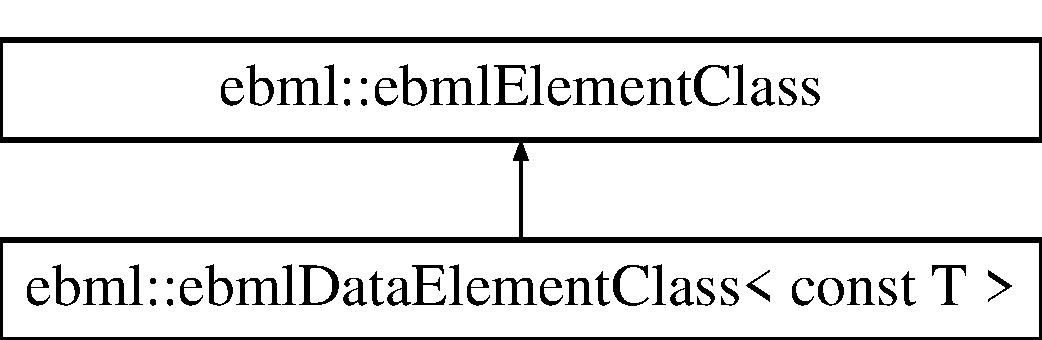
\includegraphics[height=2.000000cm]{classebml_1_1ebmlDataElementClass_3_01const_01T_01_4}
\end{center}
\end{figure}
\subsection*{Public Member Functions}
\begin{DoxyCompactItemize}
\item 
\mbox{\hyperlink{classebml_1_1ebmlDataElementClass_3_01const_01T_01_4_ad773b2b4c45bcb51ebfcba12d4888de2}{ebml\+Data\+Element\+Class}} (const char $\ast$, const std\+::wstring \&)
\item 
\mbox{\hyperlink{classebml_1_1ebmlDataElementClass_3_01const_01T_01_4_a99c231404d053be2783f12671428baa5}{ebml\+Data\+Element\+Class}} (const char $\ast$, const std\+::wstring \&, const T \&)
\item 
\mbox{\hyperlink{classebml_1_1ebmlDataElementClass_3_01const_01T_01_4_a6520906c14ba70894272b26833de66c9}{ebml\+Data\+Element\+Class}} (const char $\ast$, const std\+::wstring \&, T \&\&)
\item 
\mbox{\hyperlink{classebml_1_1ebmlDataElementClass_3_01const_01T_01_4_a83d68654ada83eb978d50133b93df485}{ebml\+Data\+Element\+Class}} (\mbox{\hyperlink{namespaceebml_a86c5f604ddf12a74aa9812e997a58691}{ebml\+I\+D\+\_\+t}}, const std\+::wstring \&)
\item 
\mbox{\hyperlink{classebml_1_1ebmlDataElementClass_3_01const_01T_01_4_afabeada87b7b2a7fd9a5944b8534cb5d}{ebml\+Data\+Element\+Class}} (\mbox{\hyperlink{namespaceebml_a86c5f604ddf12a74aa9812e997a58691}{ebml\+I\+D\+\_\+t}}, const std\+::wstring \&, const T \&)
\item 
\mbox{\hyperlink{classebml_1_1ebmlDataElementClass_3_01const_01T_01_4_a2b30da4fc5e2e00ee773db25db952704}{ebml\+Data\+Element\+Class}} (\mbox{\hyperlink{namespaceebml_a86c5f604ddf12a74aa9812e997a58691}{ebml\+I\+D\+\_\+t}}, const std\+::wstring \&, T \&\&)
\item 
virtual \mbox{\hyperlink{namespaceebml_adad533b7705a16bb360fe56380c5e7be}{ebml\+Element\+\_\+sp}} \mbox{\hyperlink{classebml_1_1ebmlDataElementClass_3_01const_01T_01_4_a7873f495e6b29cca5f3d73e0e34873f5}{operator()}} (const T \&) const
\item 
virtual \mbox{\hyperlink{namespaceebml_adad533b7705a16bb360fe56380c5e7be}{ebml\+Element\+\_\+sp}} \mbox{\hyperlink{classebml_1_1ebmlDataElementClass_3_01const_01T_01_4_ab7167a66c766cc253d32fca44856c70e}{operator()}} (T \&\&) const
\end{DoxyCompactItemize}
\subsection*{Public Attributes}
\begin{DoxyCompactItemize}
\item 
const T \mbox{\hyperlink{classebml_1_1ebmlDataElementClass_3_01const_01T_01_4_aea8b5f04ffa6327c211e20171d75fdcd}{defaultval}}
\end{DoxyCompactItemize}
\subsection*{Static Public Attributes}
\begin{DoxyCompactItemize}
\item 
static const T \mbox{\hyperlink{classebml_1_1ebmlDataElementClass_3_01const_01T_01_4_a4b0000068ea1cd6b05a45b038e47c436}{defaultdefault}}
\end{DoxyCompactItemize}
\subsection*{Protected Member Functions}
\begin{DoxyCompactItemize}
\item 
\mbox{\hyperlink{classebml_1_1ebmlElement}{ebml\+Element}} $\ast$ \mbox{\hyperlink{classebml_1_1ebmlDataElementClass_3_01const_01T_01_4_aaf6b66092e1987919e277661b62f2d90}{\+\_\+new}} () const override
\item 
\mbox{\hyperlink{namespaceebml_adad533b7705a16bb360fe56380c5e7be}{ebml\+Element\+\_\+sp}} \mbox{\hyperlink{classebml_1_1ebmlDataElementClass_3_01const_01T_01_4_a0f8a6e30cd3cc630950a780a726849a7}{\+\_\+decode}} (const \mbox{\hyperlink{classebml_1_1parseString}{parse\+String}} \&) const override
\item 
\mbox{\hyperlink{namespaceebml_adad533b7705a16bb360fe56380c5e7be}{ebml\+Element\+\_\+sp}} \mbox{\hyperlink{classebml_1_1ebmlDataElementClass_3_01const_01T_01_4_a472912867198ebff97d963cdd7f5ce33}{\+\_\+decode}} (const \mbox{\hyperlink{classebml_1_1parseFile}{parse\+File}} \&) const override
\end{DoxyCompactItemize}
\subsection*{Friends}
\begin{DoxyCompactItemize}
\item 
class \mbox{\hyperlink{classebml_1_1ebmlDataElementClass_3_01const_01T_01_4_a2cbdad6043a14b5d01294e19181e831c}{ebml\+Data\+Element$<$ const T $>$}}
\end{DoxyCompactItemize}


\subsection{Constructor \& Destructor Documentation}
\mbox{\Hypertarget{classebml_1_1ebmlDataElementClass_3_01const_01T_01_4_ad773b2b4c45bcb51ebfcba12d4888de2}\label{classebml_1_1ebmlDataElementClass_3_01const_01T_01_4_ad773b2b4c45bcb51ebfcba12d4888de2}} 
\index{ebml\+::ebml\+Data\+Element\+Class$<$ const T $>$@{ebml\+::ebml\+Data\+Element\+Class$<$ const T $>$}!ebml\+Data\+Element\+Class@{ebml\+Data\+Element\+Class}}
\index{ebml\+Data\+Element\+Class@{ebml\+Data\+Element\+Class}!ebml\+::ebml\+Data\+Element\+Class$<$ const T $>$@{ebml\+::ebml\+Data\+Element\+Class$<$ const T $>$}}
\subsubsection{\texorpdfstring{ebml\+Data\+Element\+Class()}{ebmlDataElementClass()}\hspace{0.1cm}{\footnotesize\ttfamily [1/6]}}
{\footnotesize\ttfamily template$<$typename T $>$ \\
\mbox{\hyperlink{classebml_1_1ebmlDataElementClass}{ebml\+::ebml\+Data\+Element\+Class}}$<$ const T $>$\+::\mbox{\hyperlink{classebml_1_1ebmlDataElementClass}{ebml\+Data\+Element\+Class}} (\begin{DoxyParamCaption}\item[{const char $\ast$}]{,  }\item[{const std\+::wstring \&}]{ }\end{DoxyParamCaption})}

\mbox{\Hypertarget{classebml_1_1ebmlDataElementClass_3_01const_01T_01_4_a99c231404d053be2783f12671428baa5}\label{classebml_1_1ebmlDataElementClass_3_01const_01T_01_4_a99c231404d053be2783f12671428baa5}} 
\index{ebml\+::ebml\+Data\+Element\+Class$<$ const T $>$@{ebml\+::ebml\+Data\+Element\+Class$<$ const T $>$}!ebml\+Data\+Element\+Class@{ebml\+Data\+Element\+Class}}
\index{ebml\+Data\+Element\+Class@{ebml\+Data\+Element\+Class}!ebml\+::ebml\+Data\+Element\+Class$<$ const T $>$@{ebml\+::ebml\+Data\+Element\+Class$<$ const T $>$}}
\subsubsection{\texorpdfstring{ebml\+Data\+Element\+Class()}{ebmlDataElementClass()}\hspace{0.1cm}{\footnotesize\ttfamily [2/6]}}
{\footnotesize\ttfamily template$<$typename T $>$ \\
\mbox{\hyperlink{classebml_1_1ebmlDataElementClass}{ebml\+::ebml\+Data\+Element\+Class}}$<$ const T $>$\+::\mbox{\hyperlink{classebml_1_1ebmlDataElementClass}{ebml\+Data\+Element\+Class}} (\begin{DoxyParamCaption}\item[{const char $\ast$}]{,  }\item[{const std\+::wstring \&}]{,  }\item[{const T \&}]{ }\end{DoxyParamCaption})}

\mbox{\Hypertarget{classebml_1_1ebmlDataElementClass_3_01const_01T_01_4_a6520906c14ba70894272b26833de66c9}\label{classebml_1_1ebmlDataElementClass_3_01const_01T_01_4_a6520906c14ba70894272b26833de66c9}} 
\index{ebml\+::ebml\+Data\+Element\+Class$<$ const T $>$@{ebml\+::ebml\+Data\+Element\+Class$<$ const T $>$}!ebml\+Data\+Element\+Class@{ebml\+Data\+Element\+Class}}
\index{ebml\+Data\+Element\+Class@{ebml\+Data\+Element\+Class}!ebml\+::ebml\+Data\+Element\+Class$<$ const T $>$@{ebml\+::ebml\+Data\+Element\+Class$<$ const T $>$}}
\subsubsection{\texorpdfstring{ebml\+Data\+Element\+Class()}{ebmlDataElementClass()}\hspace{0.1cm}{\footnotesize\ttfamily [3/6]}}
{\footnotesize\ttfamily template$<$typename T $>$ \\
\mbox{\hyperlink{classebml_1_1ebmlDataElementClass}{ebml\+::ebml\+Data\+Element\+Class}}$<$ const T $>$\+::\mbox{\hyperlink{classebml_1_1ebmlDataElementClass}{ebml\+Data\+Element\+Class}} (\begin{DoxyParamCaption}\item[{const char $\ast$}]{,  }\item[{const std\+::wstring \&}]{,  }\item[{T \&\&}]{ }\end{DoxyParamCaption})}

\mbox{\Hypertarget{classebml_1_1ebmlDataElementClass_3_01const_01T_01_4_a83d68654ada83eb978d50133b93df485}\label{classebml_1_1ebmlDataElementClass_3_01const_01T_01_4_a83d68654ada83eb978d50133b93df485}} 
\index{ebml\+::ebml\+Data\+Element\+Class$<$ const T $>$@{ebml\+::ebml\+Data\+Element\+Class$<$ const T $>$}!ebml\+Data\+Element\+Class@{ebml\+Data\+Element\+Class}}
\index{ebml\+Data\+Element\+Class@{ebml\+Data\+Element\+Class}!ebml\+::ebml\+Data\+Element\+Class$<$ const T $>$@{ebml\+::ebml\+Data\+Element\+Class$<$ const T $>$}}
\subsubsection{\texorpdfstring{ebml\+Data\+Element\+Class()}{ebmlDataElementClass()}\hspace{0.1cm}{\footnotesize\ttfamily [4/6]}}
{\footnotesize\ttfamily template$<$typename T $>$ \\
\mbox{\hyperlink{classebml_1_1ebmlDataElementClass}{ebml\+::ebml\+Data\+Element\+Class}}$<$ const T $>$\+::\mbox{\hyperlink{classebml_1_1ebmlDataElementClass}{ebml\+Data\+Element\+Class}} (\begin{DoxyParamCaption}\item[{\mbox{\hyperlink{namespaceebml_a86c5f604ddf12a74aa9812e997a58691}{ebml\+I\+D\+\_\+t}}}]{,  }\item[{const std\+::wstring \&}]{ }\end{DoxyParamCaption})}

\mbox{\Hypertarget{classebml_1_1ebmlDataElementClass_3_01const_01T_01_4_afabeada87b7b2a7fd9a5944b8534cb5d}\label{classebml_1_1ebmlDataElementClass_3_01const_01T_01_4_afabeada87b7b2a7fd9a5944b8534cb5d}} 
\index{ebml\+::ebml\+Data\+Element\+Class$<$ const T $>$@{ebml\+::ebml\+Data\+Element\+Class$<$ const T $>$}!ebml\+Data\+Element\+Class@{ebml\+Data\+Element\+Class}}
\index{ebml\+Data\+Element\+Class@{ebml\+Data\+Element\+Class}!ebml\+::ebml\+Data\+Element\+Class$<$ const T $>$@{ebml\+::ebml\+Data\+Element\+Class$<$ const T $>$}}
\subsubsection{\texorpdfstring{ebml\+Data\+Element\+Class()}{ebmlDataElementClass()}\hspace{0.1cm}{\footnotesize\ttfamily [5/6]}}
{\footnotesize\ttfamily template$<$typename T $>$ \\
\mbox{\hyperlink{classebml_1_1ebmlDataElementClass}{ebml\+::ebml\+Data\+Element\+Class}}$<$ const T $>$\+::\mbox{\hyperlink{classebml_1_1ebmlDataElementClass}{ebml\+Data\+Element\+Class}} (\begin{DoxyParamCaption}\item[{\mbox{\hyperlink{namespaceebml_a86c5f604ddf12a74aa9812e997a58691}{ebml\+I\+D\+\_\+t}}}]{,  }\item[{const std\+::wstring \&}]{,  }\item[{const T \&}]{ }\end{DoxyParamCaption})}

\mbox{\Hypertarget{classebml_1_1ebmlDataElementClass_3_01const_01T_01_4_a2b30da4fc5e2e00ee773db25db952704}\label{classebml_1_1ebmlDataElementClass_3_01const_01T_01_4_a2b30da4fc5e2e00ee773db25db952704}} 
\index{ebml\+::ebml\+Data\+Element\+Class$<$ const T $>$@{ebml\+::ebml\+Data\+Element\+Class$<$ const T $>$}!ebml\+Data\+Element\+Class@{ebml\+Data\+Element\+Class}}
\index{ebml\+Data\+Element\+Class@{ebml\+Data\+Element\+Class}!ebml\+::ebml\+Data\+Element\+Class$<$ const T $>$@{ebml\+::ebml\+Data\+Element\+Class$<$ const T $>$}}
\subsubsection{\texorpdfstring{ebml\+Data\+Element\+Class()}{ebmlDataElementClass()}\hspace{0.1cm}{\footnotesize\ttfamily [6/6]}}
{\footnotesize\ttfamily template$<$typename T $>$ \\
\mbox{\hyperlink{classebml_1_1ebmlDataElementClass}{ebml\+::ebml\+Data\+Element\+Class}}$<$ const T $>$\+::\mbox{\hyperlink{classebml_1_1ebmlDataElementClass}{ebml\+Data\+Element\+Class}} (\begin{DoxyParamCaption}\item[{\mbox{\hyperlink{namespaceebml_a86c5f604ddf12a74aa9812e997a58691}{ebml\+I\+D\+\_\+t}}}]{,  }\item[{const std\+::wstring \&}]{,  }\item[{T \&\&}]{ }\end{DoxyParamCaption})}



\subsection{Member Function Documentation}
\mbox{\Hypertarget{classebml_1_1ebmlDataElementClass_3_01const_01T_01_4_a0f8a6e30cd3cc630950a780a726849a7}\label{classebml_1_1ebmlDataElementClass_3_01const_01T_01_4_a0f8a6e30cd3cc630950a780a726849a7}} 
\index{ebml\+::ebml\+Data\+Element\+Class$<$ const T $>$@{ebml\+::ebml\+Data\+Element\+Class$<$ const T $>$}!\+\_\+decode@{\+\_\+decode}}
\index{\+\_\+decode@{\+\_\+decode}!ebml\+::ebml\+Data\+Element\+Class$<$ const T $>$@{ebml\+::ebml\+Data\+Element\+Class$<$ const T $>$}}
\subsubsection{\texorpdfstring{\+\_\+decode()}{\_decode()}\hspace{0.1cm}{\footnotesize\ttfamily [1/2]}}
{\footnotesize\ttfamily template$<$typename T $>$ \\
\mbox{\hyperlink{namespaceebml_adad533b7705a16bb360fe56380c5e7be}{ebml\+Element\+\_\+sp}} \mbox{\hyperlink{classebml_1_1ebmlDataElementClass}{ebml\+::ebml\+Data\+Element\+Class}}$<$ const T $>$\+::\+\_\+decode (\begin{DoxyParamCaption}\item[{const \mbox{\hyperlink{classebml_1_1parseString}{parse\+String}} \&}]{ }\end{DoxyParamCaption}) const\hspace{0.3cm}{\ttfamily [override]}, {\ttfamily [protected]}, {\ttfamily [virtual]}}



Implements \mbox{\hyperlink{classebml_1_1ebmlElementClass_aa6bf675de4918fd7b553d141871a2ede}{ebml\+::ebml\+Element\+Class}}.

\mbox{\Hypertarget{classebml_1_1ebmlDataElementClass_3_01const_01T_01_4_a472912867198ebff97d963cdd7f5ce33}\label{classebml_1_1ebmlDataElementClass_3_01const_01T_01_4_a472912867198ebff97d963cdd7f5ce33}} 
\index{ebml\+::ebml\+Data\+Element\+Class$<$ const T $>$@{ebml\+::ebml\+Data\+Element\+Class$<$ const T $>$}!\+\_\+decode@{\+\_\+decode}}
\index{\+\_\+decode@{\+\_\+decode}!ebml\+::ebml\+Data\+Element\+Class$<$ const T $>$@{ebml\+::ebml\+Data\+Element\+Class$<$ const T $>$}}
\subsubsection{\texorpdfstring{\+\_\+decode()}{\_decode()}\hspace{0.1cm}{\footnotesize\ttfamily [2/2]}}
{\footnotesize\ttfamily template$<$typename T $>$ \\
\mbox{\hyperlink{namespaceebml_adad533b7705a16bb360fe56380c5e7be}{ebml\+Element\+\_\+sp}} \mbox{\hyperlink{classebml_1_1ebmlDataElementClass}{ebml\+::ebml\+Data\+Element\+Class}}$<$ const T $>$\+::\+\_\+decode (\begin{DoxyParamCaption}\item[{const \mbox{\hyperlink{classebml_1_1parseFile}{parse\+File}} \&}]{ }\end{DoxyParamCaption}) const\hspace{0.3cm}{\ttfamily [override]}, {\ttfamily [protected]}, {\ttfamily [virtual]}}



Implements \mbox{\hyperlink{classebml_1_1ebmlElementClass_aedbfff5909af215acaa3ca28643f1bc9}{ebml\+::ebml\+Element\+Class}}.

\mbox{\Hypertarget{classebml_1_1ebmlDataElementClass_3_01const_01T_01_4_aaf6b66092e1987919e277661b62f2d90}\label{classebml_1_1ebmlDataElementClass_3_01const_01T_01_4_aaf6b66092e1987919e277661b62f2d90}} 
\index{ebml\+::ebml\+Data\+Element\+Class$<$ const T $>$@{ebml\+::ebml\+Data\+Element\+Class$<$ const T $>$}!\+\_\+new@{\+\_\+new}}
\index{\+\_\+new@{\+\_\+new}!ebml\+::ebml\+Data\+Element\+Class$<$ const T $>$@{ebml\+::ebml\+Data\+Element\+Class$<$ const T $>$}}
\subsubsection{\texorpdfstring{\+\_\+new()}{\_new()}}
{\footnotesize\ttfamily template$<$typename T $>$ \\
\mbox{\hyperlink{classebml_1_1ebmlElement}{ebml\+Element}}$\ast$ \mbox{\hyperlink{classebml_1_1ebmlDataElementClass}{ebml\+::ebml\+Data\+Element\+Class}}$<$ const T $>$\+::\+\_\+new (\begin{DoxyParamCaption}{ }\end{DoxyParamCaption}) const\hspace{0.3cm}{\ttfamily [override]}, {\ttfamily [protected]}, {\ttfamily [virtual]}}



Implements \mbox{\hyperlink{classebml_1_1ebmlElementClass_a223ede6b8bc3c85251d2d73f0256fb45}{ebml\+::ebml\+Element\+Class}}.

\mbox{\Hypertarget{classebml_1_1ebmlDataElementClass_3_01const_01T_01_4_a7873f495e6b29cca5f3d73e0e34873f5}\label{classebml_1_1ebmlDataElementClass_3_01const_01T_01_4_a7873f495e6b29cca5f3d73e0e34873f5}} 
\index{ebml\+::ebml\+Data\+Element\+Class$<$ const T $>$@{ebml\+::ebml\+Data\+Element\+Class$<$ const T $>$}!operator()@{operator()}}
\index{operator()@{operator()}!ebml\+::ebml\+Data\+Element\+Class$<$ const T $>$@{ebml\+::ebml\+Data\+Element\+Class$<$ const T $>$}}
\subsubsection{\texorpdfstring{operator()()}{operator()()}\hspace{0.1cm}{\footnotesize\ttfamily [1/2]}}
{\footnotesize\ttfamily template$<$typename T $>$ \\
virtual \mbox{\hyperlink{namespaceebml_adad533b7705a16bb360fe56380c5e7be}{ebml\+Element\+\_\+sp}} \mbox{\hyperlink{classebml_1_1ebmlDataElementClass}{ebml\+::ebml\+Data\+Element\+Class}}$<$ const T $>$\+::operator() (\begin{DoxyParamCaption}\item[{const T \&}]{ }\end{DoxyParamCaption}) const\hspace{0.3cm}{\ttfamily [virtual]}}

\mbox{\Hypertarget{classebml_1_1ebmlDataElementClass_3_01const_01T_01_4_ab7167a66c766cc253d32fca44856c70e}\label{classebml_1_1ebmlDataElementClass_3_01const_01T_01_4_ab7167a66c766cc253d32fca44856c70e}} 
\index{ebml\+::ebml\+Data\+Element\+Class$<$ const T $>$@{ebml\+::ebml\+Data\+Element\+Class$<$ const T $>$}!operator()@{operator()}}
\index{operator()@{operator()}!ebml\+::ebml\+Data\+Element\+Class$<$ const T $>$@{ebml\+::ebml\+Data\+Element\+Class$<$ const T $>$}}
\subsubsection{\texorpdfstring{operator()()}{operator()()}\hspace{0.1cm}{\footnotesize\ttfamily [2/2]}}
{\footnotesize\ttfamily template$<$typename T $>$ \\
virtual \mbox{\hyperlink{namespaceebml_adad533b7705a16bb360fe56380c5e7be}{ebml\+Element\+\_\+sp}} \mbox{\hyperlink{classebml_1_1ebmlDataElementClass}{ebml\+::ebml\+Data\+Element\+Class}}$<$ const T $>$\+::operator() (\begin{DoxyParamCaption}\item[{T \&\&}]{ }\end{DoxyParamCaption}) const\hspace{0.3cm}{\ttfamily [virtual]}}



\subsection{Friends And Related Function Documentation}
\mbox{\Hypertarget{classebml_1_1ebmlDataElementClass_3_01const_01T_01_4_a2cbdad6043a14b5d01294e19181e831c}\label{classebml_1_1ebmlDataElementClass_3_01const_01T_01_4_a2cbdad6043a14b5d01294e19181e831c}} 
\index{ebml\+::ebml\+Data\+Element\+Class$<$ const T $>$@{ebml\+::ebml\+Data\+Element\+Class$<$ const T $>$}!ebml\+Data\+Element$<$ const T $>$@{ebml\+Data\+Element$<$ const T $>$}}
\index{ebml\+Data\+Element$<$ const T $>$@{ebml\+Data\+Element$<$ const T $>$}!ebml\+::ebml\+Data\+Element\+Class$<$ const T $>$@{ebml\+::ebml\+Data\+Element\+Class$<$ const T $>$}}
\subsubsection{\texorpdfstring{ebml\+Data\+Element$<$ const T $>$}{ebmlDataElement< const T >}}
{\footnotesize\ttfamily template$<$typename T $>$ \\
friend class \mbox{\hyperlink{classebml_1_1ebmlDataElement}{ebml\+Data\+Element}}$<$ const T $>$\hspace{0.3cm}{\ttfamily [friend]}}



\subsection{Member Data Documentation}
\mbox{\Hypertarget{classebml_1_1ebmlDataElementClass_3_01const_01T_01_4_a4b0000068ea1cd6b05a45b038e47c436}\label{classebml_1_1ebmlDataElementClass_3_01const_01T_01_4_a4b0000068ea1cd6b05a45b038e47c436}} 
\index{ebml\+::ebml\+Data\+Element\+Class$<$ const T $>$@{ebml\+::ebml\+Data\+Element\+Class$<$ const T $>$}!defaultdefault@{defaultdefault}}
\index{defaultdefault@{defaultdefault}!ebml\+::ebml\+Data\+Element\+Class$<$ const T $>$@{ebml\+::ebml\+Data\+Element\+Class$<$ const T $>$}}
\subsubsection{\texorpdfstring{defaultdefault}{defaultdefault}}
{\footnotesize\ttfamily template$<$typename T $>$ \\
const T \mbox{\hyperlink{classebml_1_1ebmlDataElementClass}{ebml\+::ebml\+Data\+Element\+Class}}$<$ const T $>$\+::defaultdefault\hspace{0.3cm}{\ttfamily [static]}}

\mbox{\Hypertarget{classebml_1_1ebmlDataElementClass_3_01const_01T_01_4_aea8b5f04ffa6327c211e20171d75fdcd}\label{classebml_1_1ebmlDataElementClass_3_01const_01T_01_4_aea8b5f04ffa6327c211e20171d75fdcd}} 
\index{ebml\+::ebml\+Data\+Element\+Class$<$ const T $>$@{ebml\+::ebml\+Data\+Element\+Class$<$ const T $>$}!defaultval@{defaultval}}
\index{defaultval@{defaultval}!ebml\+::ebml\+Data\+Element\+Class$<$ const T $>$@{ebml\+::ebml\+Data\+Element\+Class$<$ const T $>$}}
\subsubsection{\texorpdfstring{defaultval}{defaultval}}
{\footnotesize\ttfamily template$<$typename T $>$ \\
const T \mbox{\hyperlink{classebml_1_1ebmlDataElementClass}{ebml\+::ebml\+Data\+Element\+Class}}$<$ const T $>$\+::defaultval}



The documentation for this class was generated from the following file\+:\begin{DoxyCompactItemize}
\item 
include/libebml\+\_\+ng/\mbox{\hyperlink{dataelement_8h}{dataelement.\+h}}\end{DoxyCompactItemize}

\hypertarget{classebml_1_1ebmlDecodeError}{}\section{ebml\+:\+:ebml\+Decode\+Error Class Reference}
\label{classebml_1_1ebmlDecodeError}\index{ebml\+::ebml\+Decode\+Error@{ebml\+::ebml\+Decode\+Error}}


{\ttfamily \#include $<$exceptions.\+h$>$}

Inheritance diagram for ebml\+:\+:ebml\+Decode\+Error\+:\begin{figure}[H]
\begin{center}
\leavevmode
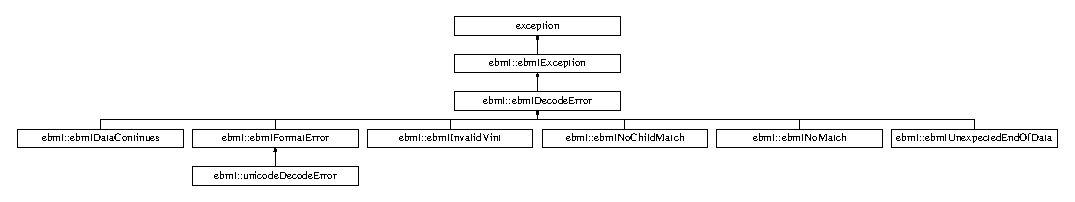
\includegraphics[height=2.265372cm]{classebml_1_1ebmlDecodeError}
\end{center}
\end{figure}
\subsection*{Public Member Functions}
\begin{DoxyCompactItemize}
\item 
\mbox{\hyperlink{classebml_1_1ebmlDecodeError_a1b644d8b9774ec88685fcedf87cdd74f}{ebml\+Decode\+Error}} (const std\+::string \&message, const \mbox{\hyperlink{classebml_1_1ebmlElementClass}{ebml\+Element\+Class}} $\ast$\mbox{\hyperlink{classebml_1_1ebmlDecodeError_a3568b4ea3cd5bd16b9510abfe269920f}{cls}}=nullptr, off\+\_\+t \mbox{\hyperlink{classebml_1_1ebmlDecodeError_ad32ac9b3dd52f1c11479085d9c665e0f}{offset}}=-\/1, unsigned char \mbox{\hyperlink{classebml_1_1ebmlDecodeError_a61a4d4856f0c779a1c216e45dc5a7c1e}{head\+Size}}=0, off\+\_\+t \mbox{\hyperlink{classebml_1_1ebmlDecodeError_acb525117e0109d9640fb5e8c546e9a02}{erroroffset}}=-\/1)
\item 
virtual void \mbox{\hyperlink{classebml_1_1ebmlDecodeError_a2ff987918cff7b3495e2f9583087518d}{add\+\_\+to\+\_\+offset}} (off\+\_\+t)
\end{DoxyCompactItemize}
\subsection*{Public Attributes}
\begin{DoxyCompactItemize}
\item 
off\+\_\+t \mbox{\hyperlink{classebml_1_1ebmlDecodeError_ad32ac9b3dd52f1c11479085d9c665e0f}{offset}}
\item 
unsigned char \mbox{\hyperlink{classebml_1_1ebmlDecodeError_a61a4d4856f0c779a1c216e45dc5a7c1e}{head\+Size}}
\item 
off\+\_\+t \mbox{\hyperlink{classebml_1_1ebmlDecodeError_acb525117e0109d9640fb5e8c546e9a02}{erroroffset}}
\item 
const \mbox{\hyperlink{classebml_1_1ebmlElementClass}{ebml\+Element\+Class}} $\ast$ \mbox{\hyperlink{classebml_1_1ebmlDecodeError_a3568b4ea3cd5bd16b9510abfe269920f}{cls}}
\end{DoxyCompactItemize}


\subsection{Constructor \& Destructor Documentation}
\mbox{\Hypertarget{classebml_1_1ebmlDecodeError_a1b644d8b9774ec88685fcedf87cdd74f}\label{classebml_1_1ebmlDecodeError_a1b644d8b9774ec88685fcedf87cdd74f}} 
\index{ebml\+::ebml\+Decode\+Error@{ebml\+::ebml\+Decode\+Error}!ebml\+Decode\+Error@{ebml\+Decode\+Error}}
\index{ebml\+Decode\+Error@{ebml\+Decode\+Error}!ebml\+::ebml\+Decode\+Error@{ebml\+::ebml\+Decode\+Error}}
\subsubsection{\texorpdfstring{ebml\+Decode\+Error()}{ebmlDecodeError()}}
{\footnotesize\ttfamily ebml\+::ebml\+Decode\+Error\+::ebml\+Decode\+Error (\begin{DoxyParamCaption}\item[{const std\+::string \&}]{message,  }\item[{const \mbox{\hyperlink{classebml_1_1ebmlElementClass}{ebml\+Element\+Class}} $\ast$}]{cls = {\ttfamily nullptr},  }\item[{off\+\_\+t}]{offset = {\ttfamily -\/1},  }\item[{unsigned char}]{head\+Size = {\ttfamily 0},  }\item[{off\+\_\+t}]{erroroffset = {\ttfamily -\/1} }\end{DoxyParamCaption})}



\subsection{Member Function Documentation}
\mbox{\Hypertarget{classebml_1_1ebmlDecodeError_a2ff987918cff7b3495e2f9583087518d}\label{classebml_1_1ebmlDecodeError_a2ff987918cff7b3495e2f9583087518d}} 
\index{ebml\+::ebml\+Decode\+Error@{ebml\+::ebml\+Decode\+Error}!add\+\_\+to\+\_\+offset@{add\+\_\+to\+\_\+offset}}
\index{add\+\_\+to\+\_\+offset@{add\+\_\+to\+\_\+offset}!ebml\+::ebml\+Decode\+Error@{ebml\+::ebml\+Decode\+Error}}
\subsubsection{\texorpdfstring{add\+\_\+to\+\_\+offset()}{add\_to\_offset()}}
{\footnotesize\ttfamily virtual void ebml\+::ebml\+Decode\+Error\+::add\+\_\+to\+\_\+offset (\begin{DoxyParamCaption}\item[{off\+\_\+t}]{ }\end{DoxyParamCaption})\hspace{0.3cm}{\ttfamily [virtual]}}



\subsection{Member Data Documentation}
\mbox{\Hypertarget{classebml_1_1ebmlDecodeError_a3568b4ea3cd5bd16b9510abfe269920f}\label{classebml_1_1ebmlDecodeError_a3568b4ea3cd5bd16b9510abfe269920f}} 
\index{ebml\+::ebml\+Decode\+Error@{ebml\+::ebml\+Decode\+Error}!cls@{cls}}
\index{cls@{cls}!ebml\+::ebml\+Decode\+Error@{ebml\+::ebml\+Decode\+Error}}
\subsubsection{\texorpdfstring{cls}{cls}}
{\footnotesize\ttfamily const \mbox{\hyperlink{classebml_1_1ebmlElementClass}{ebml\+Element\+Class}}$\ast$ ebml\+::ebml\+Decode\+Error\+::cls}

\mbox{\Hypertarget{classebml_1_1ebmlDecodeError_acb525117e0109d9640fb5e8c546e9a02}\label{classebml_1_1ebmlDecodeError_acb525117e0109d9640fb5e8c546e9a02}} 
\index{ebml\+::ebml\+Decode\+Error@{ebml\+::ebml\+Decode\+Error}!erroroffset@{erroroffset}}
\index{erroroffset@{erroroffset}!ebml\+::ebml\+Decode\+Error@{ebml\+::ebml\+Decode\+Error}}
\subsubsection{\texorpdfstring{erroroffset}{erroroffset}}
{\footnotesize\ttfamily off\+\_\+t ebml\+::ebml\+Decode\+Error\+::erroroffset}

\mbox{\Hypertarget{classebml_1_1ebmlDecodeError_a61a4d4856f0c779a1c216e45dc5a7c1e}\label{classebml_1_1ebmlDecodeError_a61a4d4856f0c779a1c216e45dc5a7c1e}} 
\index{ebml\+::ebml\+Decode\+Error@{ebml\+::ebml\+Decode\+Error}!head\+Size@{head\+Size}}
\index{head\+Size@{head\+Size}!ebml\+::ebml\+Decode\+Error@{ebml\+::ebml\+Decode\+Error}}
\subsubsection{\texorpdfstring{head\+Size}{headSize}}
{\footnotesize\ttfamily unsigned char ebml\+::ebml\+Decode\+Error\+::head\+Size}

\mbox{\Hypertarget{classebml_1_1ebmlDecodeError_ad32ac9b3dd52f1c11479085d9c665e0f}\label{classebml_1_1ebmlDecodeError_ad32ac9b3dd52f1c11479085d9c665e0f}} 
\index{ebml\+::ebml\+Decode\+Error@{ebml\+::ebml\+Decode\+Error}!offset@{offset}}
\index{offset@{offset}!ebml\+::ebml\+Decode\+Error@{ebml\+::ebml\+Decode\+Error}}
\subsubsection{\texorpdfstring{offset}{offset}}
{\footnotesize\ttfamily off\+\_\+t ebml\+::ebml\+Decode\+Error\+::offset}



The documentation for this class was generated from the following file\+:\begin{DoxyCompactItemize}
\item 
include/libebml\+\_\+ng/\mbox{\hyperlink{exceptions_8h}{exceptions.\+h}}\end{DoxyCompactItemize}

\hypertarget{classebml_1_1ebmlDocument}{}\section{ebml\+:\+:ebml\+Document Class Reference}
\label{classebml_1_1ebmlDocument}\index{ebml\+::ebml\+Document@{ebml\+::ebml\+Document}}


{\ttfamily \#include $<$document.\+h$>$}

Inheritance diagram for ebml\+:\+:ebml\+Document\+:\begin{figure}[H]
\begin{center}
\leavevmode
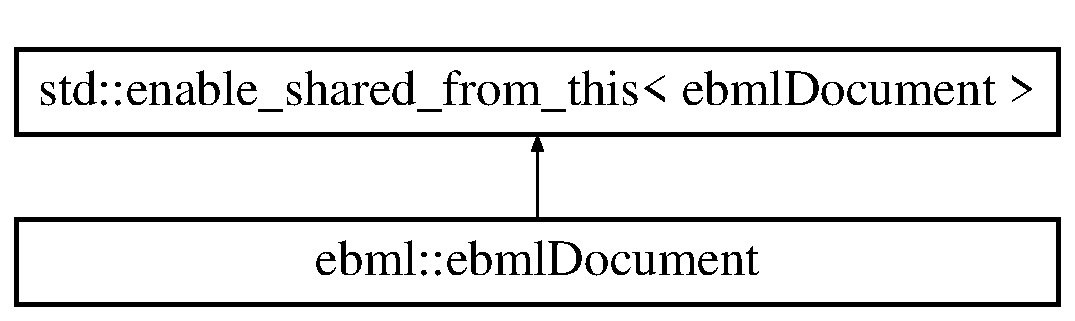
\includegraphics[height=2.000000cm]{classebml_1_1ebmlDocument}
\end{center}
\end{figure}
\subsection*{Public Member Functions}
\begin{DoxyCompactItemize}
\item 
const \mbox{\hyperlink{namespaceebml_a7bb59128ac6af27e47367938a846b569}{io\+Base\+\_\+sp}} \& \mbox{\hyperlink{classebml_1_1ebmlDocument_ab95de6cd5be1fbeefb5a50cc001c42cc}{file}} ()
\item 
const \mbox{\hyperlink{namespaceebml_adad533b7705a16bb360fe56380c5e7be}{ebml\+Element\+\_\+sp}} \& \mbox{\hyperlink{classebml_1_1ebmlDocument_a012478219e8197111084ba55dc0586a5}{root}} () const
\item 
const \mbox{\hyperlink{namespaceebml_adad533b7705a16bb360fe56380c5e7be}{ebml\+Element\+\_\+sp}} \& \mbox{\hyperlink{classebml_1_1ebmlDocument_addbc9eaabb0d2a608b6a19e4f7b5e17b}{head}} () const
\item 
const \mbox{\hyperlink{classebml_1_1ebmlSchema}{ebml\+Schema}} $\ast$ \mbox{\hyperlink{classebml_1_1ebmlDocument_aff3d1abece0a2bedf5a90e6af0ff3ddd}{schema}} () const
\end{DoxyCompactItemize}
\subsection*{Protected Member Functions}
\begin{DoxyCompactItemize}
\item 
\mbox{\hyperlink{classebml_1_1ebmlDocument_a7ad723caca4bea0c0991e3e3dd102c7d}{ebml\+Document}} (const \mbox{\hyperlink{classebml_1_1ebmlSchema}{ebml\+Schema}} $\ast$)
\item 
\mbox{\hyperlink{classebml_1_1ebmlDocument_a3bc6d62192147a62deee0684ab9c3939}{ebml\+Document}} (const \mbox{\hyperlink{classebml_1_1ebmlSchema}{ebml\+Schema}} $\ast$, const \mbox{\hyperlink{namespaceebml_a7bb59128ac6af27e47367938a846b569}{io\+Base\+\_\+sp}} \&)
\item 
\mbox{\hyperlink{classebml_1_1ebmlDocument_a2c834b20ecc9613ceb585f735cd3162c}{ebml\+Document}} (const \mbox{\hyperlink{classebml_1_1ebmlSchema}{ebml\+Schema}} $\ast$, \mbox{\hyperlink{namespaceebml_a7bb59128ac6af27e47367938a846b569}{io\+Base\+\_\+sp}} \&\&)
\item 
void \mbox{\hyperlink{classebml_1_1ebmlDocument_ad61feb3fb9966a0b3b9d2f5f5cdd4dd0}{set\+Head}} (const \mbox{\hyperlink{namespaceebml_adad533b7705a16bb360fe56380c5e7be}{ebml\+Element\+\_\+sp}} \&)
\item 
void \mbox{\hyperlink{classebml_1_1ebmlDocument_add439a24bc460b0a3ece976003c865c1}{set\+Head}} (\mbox{\hyperlink{namespaceebml_adad533b7705a16bb360fe56380c5e7be}{ebml\+Element\+\_\+sp}} \&\&)
\item 
void \mbox{\hyperlink{classebml_1_1ebmlDocument_ab845edd17a23f956d0fd9461a26053cd}{set\+Root}} (const \mbox{\hyperlink{namespaceebml_adad533b7705a16bb360fe56380c5e7be}{ebml\+Element\+\_\+sp}} \&)
\item 
void \mbox{\hyperlink{classebml_1_1ebmlDocument_a709554a561abcbb47f51a14c59682c74}{set\+Root}} (\mbox{\hyperlink{namespaceebml_adad533b7705a16bb360fe56380c5e7be}{ebml\+Element\+\_\+sp}} \&\&)
\end{DoxyCompactItemize}
\subsection*{Friends}
\begin{DoxyCompactItemize}
\item 
class \mbox{\hyperlink{classebml_1_1ebmlDocument_ab99d947c503dbe1ab7ebb0a75c24e4df}{ebml\+Schema}}
\end{DoxyCompactItemize}


\subsection{Constructor \& Destructor Documentation}
\mbox{\Hypertarget{classebml_1_1ebmlDocument_a7ad723caca4bea0c0991e3e3dd102c7d}\label{classebml_1_1ebmlDocument_a7ad723caca4bea0c0991e3e3dd102c7d}} 
\index{ebml\+::ebml\+Document@{ebml\+::ebml\+Document}!ebml\+Document@{ebml\+Document}}
\index{ebml\+Document@{ebml\+Document}!ebml\+::ebml\+Document@{ebml\+::ebml\+Document}}
\subsubsection{\texorpdfstring{ebml\+Document()}{ebmlDocument()}\hspace{0.1cm}{\footnotesize\ttfamily [1/3]}}
{\footnotesize\ttfamily ebml\+::ebml\+Document\+::ebml\+Document (\begin{DoxyParamCaption}\item[{const \mbox{\hyperlink{classebml_1_1ebmlSchema}{ebml\+Schema}} $\ast$}]{ }\end{DoxyParamCaption})\hspace{0.3cm}{\ttfamily [protected]}}

\mbox{\Hypertarget{classebml_1_1ebmlDocument_a3bc6d62192147a62deee0684ab9c3939}\label{classebml_1_1ebmlDocument_a3bc6d62192147a62deee0684ab9c3939}} 
\index{ebml\+::ebml\+Document@{ebml\+::ebml\+Document}!ebml\+Document@{ebml\+Document}}
\index{ebml\+Document@{ebml\+Document}!ebml\+::ebml\+Document@{ebml\+::ebml\+Document}}
\subsubsection{\texorpdfstring{ebml\+Document()}{ebmlDocument()}\hspace{0.1cm}{\footnotesize\ttfamily [2/3]}}
{\footnotesize\ttfamily ebml\+::ebml\+Document\+::ebml\+Document (\begin{DoxyParamCaption}\item[{const \mbox{\hyperlink{classebml_1_1ebmlSchema}{ebml\+Schema}} $\ast$}]{,  }\item[{const \mbox{\hyperlink{namespaceebml_a7bb59128ac6af27e47367938a846b569}{io\+Base\+\_\+sp}} \&}]{ }\end{DoxyParamCaption})\hspace{0.3cm}{\ttfamily [protected]}}

\mbox{\Hypertarget{classebml_1_1ebmlDocument_a2c834b20ecc9613ceb585f735cd3162c}\label{classebml_1_1ebmlDocument_a2c834b20ecc9613ceb585f735cd3162c}} 
\index{ebml\+::ebml\+Document@{ebml\+::ebml\+Document}!ebml\+Document@{ebml\+Document}}
\index{ebml\+Document@{ebml\+Document}!ebml\+::ebml\+Document@{ebml\+::ebml\+Document}}
\subsubsection{\texorpdfstring{ebml\+Document()}{ebmlDocument()}\hspace{0.1cm}{\footnotesize\ttfamily [3/3]}}
{\footnotesize\ttfamily ebml\+::ebml\+Document\+::ebml\+Document (\begin{DoxyParamCaption}\item[{const \mbox{\hyperlink{classebml_1_1ebmlSchema}{ebml\+Schema}} $\ast$}]{,  }\item[{\mbox{\hyperlink{namespaceebml_a7bb59128ac6af27e47367938a846b569}{io\+Base\+\_\+sp}} \&\&}]{ }\end{DoxyParamCaption})\hspace{0.3cm}{\ttfamily [protected]}}



\subsection{Member Function Documentation}
\mbox{\Hypertarget{classebml_1_1ebmlDocument_ab95de6cd5be1fbeefb5a50cc001c42cc}\label{classebml_1_1ebmlDocument_ab95de6cd5be1fbeefb5a50cc001c42cc}} 
\index{ebml\+::ebml\+Document@{ebml\+::ebml\+Document}!file@{file}}
\index{file@{file}!ebml\+::ebml\+Document@{ebml\+::ebml\+Document}}
\subsubsection{\texorpdfstring{file()}{file()}}
{\footnotesize\ttfamily const \mbox{\hyperlink{namespaceebml_a7bb59128ac6af27e47367938a846b569}{io\+Base\+\_\+sp}}\& ebml\+::ebml\+Document\+::file (\begin{DoxyParamCaption}{ }\end{DoxyParamCaption})}

\mbox{\Hypertarget{classebml_1_1ebmlDocument_addbc9eaabb0d2a608b6a19e4f7b5e17b}\label{classebml_1_1ebmlDocument_addbc9eaabb0d2a608b6a19e4f7b5e17b}} 
\index{ebml\+::ebml\+Document@{ebml\+::ebml\+Document}!head@{head}}
\index{head@{head}!ebml\+::ebml\+Document@{ebml\+::ebml\+Document}}
\subsubsection{\texorpdfstring{head()}{head()}}
{\footnotesize\ttfamily const \mbox{\hyperlink{namespaceebml_adad533b7705a16bb360fe56380c5e7be}{ebml\+Element\+\_\+sp}}\& ebml\+::ebml\+Document\+::head (\begin{DoxyParamCaption}{ }\end{DoxyParamCaption}) const}

\mbox{\Hypertarget{classebml_1_1ebmlDocument_a012478219e8197111084ba55dc0586a5}\label{classebml_1_1ebmlDocument_a012478219e8197111084ba55dc0586a5}} 
\index{ebml\+::ebml\+Document@{ebml\+::ebml\+Document}!root@{root}}
\index{root@{root}!ebml\+::ebml\+Document@{ebml\+::ebml\+Document}}
\subsubsection{\texorpdfstring{root()}{root()}}
{\footnotesize\ttfamily const \mbox{\hyperlink{namespaceebml_adad533b7705a16bb360fe56380c5e7be}{ebml\+Element\+\_\+sp}}\& ebml\+::ebml\+Document\+::root (\begin{DoxyParamCaption}{ }\end{DoxyParamCaption}) const}

\mbox{\Hypertarget{classebml_1_1ebmlDocument_aff3d1abece0a2bedf5a90e6af0ff3ddd}\label{classebml_1_1ebmlDocument_aff3d1abece0a2bedf5a90e6af0ff3ddd}} 
\index{ebml\+::ebml\+Document@{ebml\+::ebml\+Document}!schema@{schema}}
\index{schema@{schema}!ebml\+::ebml\+Document@{ebml\+::ebml\+Document}}
\subsubsection{\texorpdfstring{schema()}{schema()}}
{\footnotesize\ttfamily const \mbox{\hyperlink{classebml_1_1ebmlSchema}{ebml\+Schema}}$\ast$ ebml\+::ebml\+Document\+::schema (\begin{DoxyParamCaption}{ }\end{DoxyParamCaption}) const}

\mbox{\Hypertarget{classebml_1_1ebmlDocument_ad61feb3fb9966a0b3b9d2f5f5cdd4dd0}\label{classebml_1_1ebmlDocument_ad61feb3fb9966a0b3b9d2f5f5cdd4dd0}} 
\index{ebml\+::ebml\+Document@{ebml\+::ebml\+Document}!set\+Head@{set\+Head}}
\index{set\+Head@{set\+Head}!ebml\+::ebml\+Document@{ebml\+::ebml\+Document}}
\subsubsection{\texorpdfstring{set\+Head()}{setHead()}\hspace{0.1cm}{\footnotesize\ttfamily [1/2]}}
{\footnotesize\ttfamily void ebml\+::ebml\+Document\+::set\+Head (\begin{DoxyParamCaption}\item[{const \mbox{\hyperlink{namespaceebml_adad533b7705a16bb360fe56380c5e7be}{ebml\+Element\+\_\+sp}} \&}]{ }\end{DoxyParamCaption})\hspace{0.3cm}{\ttfamily [inline]}, {\ttfamily [protected]}}

\mbox{\Hypertarget{classebml_1_1ebmlDocument_add439a24bc460b0a3ece976003c865c1}\label{classebml_1_1ebmlDocument_add439a24bc460b0a3ece976003c865c1}} 
\index{ebml\+::ebml\+Document@{ebml\+::ebml\+Document}!set\+Head@{set\+Head}}
\index{set\+Head@{set\+Head}!ebml\+::ebml\+Document@{ebml\+::ebml\+Document}}
\subsubsection{\texorpdfstring{set\+Head()}{setHead()}\hspace{0.1cm}{\footnotesize\ttfamily [2/2]}}
{\footnotesize\ttfamily void ebml\+::ebml\+Document\+::set\+Head (\begin{DoxyParamCaption}\item[{\mbox{\hyperlink{namespaceebml_adad533b7705a16bb360fe56380c5e7be}{ebml\+Element\+\_\+sp}} \&\&}]{ }\end{DoxyParamCaption})\hspace{0.3cm}{\ttfamily [protected]}}

\mbox{\Hypertarget{classebml_1_1ebmlDocument_ab845edd17a23f956d0fd9461a26053cd}\label{classebml_1_1ebmlDocument_ab845edd17a23f956d0fd9461a26053cd}} 
\index{ebml\+::ebml\+Document@{ebml\+::ebml\+Document}!set\+Root@{set\+Root}}
\index{set\+Root@{set\+Root}!ebml\+::ebml\+Document@{ebml\+::ebml\+Document}}
\subsubsection{\texorpdfstring{set\+Root()}{setRoot()}\hspace{0.1cm}{\footnotesize\ttfamily [1/2]}}
{\footnotesize\ttfamily void ebml\+::ebml\+Document\+::set\+Root (\begin{DoxyParamCaption}\item[{const \mbox{\hyperlink{namespaceebml_adad533b7705a16bb360fe56380c5e7be}{ebml\+Element\+\_\+sp}} \&}]{ }\end{DoxyParamCaption})\hspace{0.3cm}{\ttfamily [inline]}, {\ttfamily [protected]}}

\mbox{\Hypertarget{classebml_1_1ebmlDocument_a709554a561abcbb47f51a14c59682c74}\label{classebml_1_1ebmlDocument_a709554a561abcbb47f51a14c59682c74}} 
\index{ebml\+::ebml\+Document@{ebml\+::ebml\+Document}!set\+Root@{set\+Root}}
\index{set\+Root@{set\+Root}!ebml\+::ebml\+Document@{ebml\+::ebml\+Document}}
\subsubsection{\texorpdfstring{set\+Root()}{setRoot()}\hspace{0.1cm}{\footnotesize\ttfamily [2/2]}}
{\footnotesize\ttfamily void ebml\+::ebml\+Document\+::set\+Root (\begin{DoxyParamCaption}\item[{\mbox{\hyperlink{namespaceebml_adad533b7705a16bb360fe56380c5e7be}{ebml\+Element\+\_\+sp}} \&\&}]{ }\end{DoxyParamCaption})\hspace{0.3cm}{\ttfamily [protected]}}



\subsection{Friends And Related Function Documentation}
\mbox{\Hypertarget{classebml_1_1ebmlDocument_ab99d947c503dbe1ab7ebb0a75c24e4df}\label{classebml_1_1ebmlDocument_ab99d947c503dbe1ab7ebb0a75c24e4df}} 
\index{ebml\+::ebml\+Document@{ebml\+::ebml\+Document}!ebml\+Schema@{ebml\+Schema}}
\index{ebml\+Schema@{ebml\+Schema}!ebml\+::ebml\+Document@{ebml\+::ebml\+Document}}
\subsubsection{\texorpdfstring{ebml\+Schema}{ebmlSchema}}
{\footnotesize\ttfamily friend class \mbox{\hyperlink{classebml_1_1ebmlSchema}{ebml\+Schema}}\hspace{0.3cm}{\ttfamily [friend]}}



The documentation for this class was generated from the following file\+:\begin{DoxyCompactItemize}
\item 
include/libebml\+\_\+ng/\mbox{\hyperlink{document_8h}{document.\+h}}\end{DoxyCompactItemize}

\hypertarget{classebml_1_1ebmlElement}{}\section{ebml\+:\+:ebml\+Element Class Reference}
\label{classebml_1_1ebmlElement}\index{ebml\+::ebml\+Element@{ebml\+::ebml\+Element}}


{\ttfamily \#include $<$base.\+h$>$}

Inheritance diagram for ebml\+:\+:ebml\+Element\+:\begin{figure}[H]
\begin{center}
\leavevmode
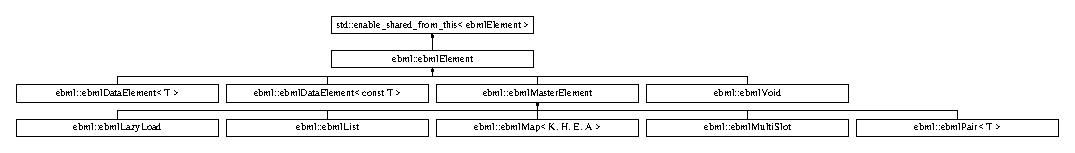
\includegraphics[height=1.611511cm]{classebml_1_1ebmlElement}
\end{center}
\end{figure}
\subsection*{Public Member Functions}
\begin{DoxyCompactItemize}
\item 
virtual \mbox{\hyperlink{classebml_1_1ebmlElement_a2098d59a92f38d5ab5dbad0c7611115a}{$\sim$ebml\+Element}} ()
\item 
virtual const \mbox{\hyperlink{classebml_1_1ebmlElementClass}{ebml\+Element\+Class}} $\ast$ \mbox{\hyperlink{classebml_1_1ebmlElement_a15cf59e94b01e2c49ec96512b9bd9d90}{cls}} () const
\item 
\mbox{\hyperlink{namespaceebml_a86c5f604ddf12a74aa9812e997a58691}{ebml\+I\+D\+\_\+t}} \mbox{\hyperlink{classebml_1_1ebmlElement_afb2aa40757e663892d3a079de0f4e7d6}{ebml\+ID}} () const
\item 
{\footnotesize template$<$typename T  = ebml\+Element$>$ }\\T \& \mbox{\hyperlink{classebml_1_1ebmlElement_a445d4f6f882750005167411c4f7f24bf}{ref}} ()
\item 
{\footnotesize template$<$typename T  = ebml\+Element$>$ }\\const T \& \mbox{\hyperlink{classebml_1_1ebmlElement_aa2679e147ba5fdf83a0da3efd090593f}{ref}} () const
\item 
{\footnotesize template$<$typename T  = ebml\+Element$>$ }\\T $\ast$ \mbox{\hyperlink{classebml_1_1ebmlElement_a974c7505c6847f3e7411cbe7dbc91f50}{ptr}} ()
\item 
{\footnotesize template$<$typename T  = ebml\+Element$>$ }\\const T $\ast$ \mbox{\hyperlink{classebml_1_1ebmlElement_a22297ffc67936033818a65c89f3564c0}{ptr}} () const
\item 
bool \mbox{\hyperlink{classebml_1_1ebmlElement_a2284de40bfd5b67a7668066a0f816296}{parent\+\_\+is\+\_\+const}} () const
\item 
\mbox{\hyperlink{namespaceebml_adad533b7705a16bb360fe56380c5e7be}{ebml\+Element\+\_\+sp}} \mbox{\hyperlink{classebml_1_1ebmlElement_a7b47b4c43f09c62f56ba326b906fe718}{parent}} () const
\item 
\mbox{\hyperlink{namespaceebml_a2deef4e8071531b32e3533f1bf978917}{c\+\_\+ebml\+Element\+\_\+sp}} \mbox{\hyperlink{classebml_1_1ebmlElement_a1254e41a77ff0157b76db8f33ad7d229}{c\+\_\+parent}} () const
\item 
\mbox{\hyperlink{namespaceebml_adad533b7705a16bb360fe56380c5e7be}{ebml\+Element\+\_\+sp}} \mbox{\hyperlink{classebml_1_1ebmlElement_a9c9ed1823c036c8a77a64c68e12e769f}{root}} () const
\item 
\mbox{\hyperlink{namespaceebml_a2deef4e8071531b32e3533f1bf978917}{c\+\_\+ebml\+Element\+\_\+sp}} \mbox{\hyperlink{classebml_1_1ebmlElement_a3dddd3edbb6c96b8765107fccad5826b}{c\+\_\+root}} () const
\item 
\mbox{\hyperlink{namespaceebml_a66018942b568da5041136a945148b450}{ebml\+Document\+\_\+sp}} \mbox{\hyperlink{classebml_1_1ebmlElement_a1ee44e2978cd9e23c98cd9c05dd8fa35}{document}} () const
\item 
bool \mbox{\hyperlink{classebml_1_1ebmlElement_a9a784c3c424216ecd4b320e2cfc713b2}{has\+Parent}} () const
\item 
unsigned char \mbox{\hyperlink{classebml_1_1ebmlElement_a9305dc06339d900f81bd986653457e28}{head\+Size}} () const
\item 
unsigned char \mbox{\hyperlink{classebml_1_1ebmlElement_a87e926e72a5c1280b674573256dc08b1}{head\+Size}} (size\+\_\+t) const
\item 
size\+\_\+t \mbox{\hyperlink{classebml_1_1ebmlElement_aa6e265beb13dae353d75cdacc77748e1}{outer\+Size}} () const
\item 
size\+\_\+t \mbox{\hyperlink{classebml_1_1ebmlElement_ac482f4483500dbe1b9042350ee81c1be}{outer\+Size}} (size\+\_\+t) const
\item 
virtual size\+\_\+t \mbox{\hyperlink{classebml_1_1ebmlElement_a47ed4167d9c69104e02b6dbad0cd1fef}{data\+Size}} () const =0
\item 
off\+\_\+t \mbox{\hyperlink{classebml_1_1ebmlElement_a06ea720b5bd804288a8d36a36cf6b6a7}{offset\+In\+Parent}} ()
\item 
off\+\_\+t \mbox{\hyperlink{classebml_1_1ebmlElement_abcb13644652965ed7cfcd1c023569b1c}{offset\+In\+File}} ()
\item 
off\+\_\+t \mbox{\hyperlink{classebml_1_1ebmlElement_a0304c2cdd1694a706d8846e596d15ec6}{data\+Offset\+In\+Parent}} ()
\item 
off\+\_\+t \mbox{\hyperlink{classebml_1_1ebmlElement_a725798d0e8cee171475f133fa36b3324}{data\+Offset\+In\+File}} ()
\item 
virtual std\+::string \mbox{\hyperlink{classebml_1_1ebmlElement_aaeddd5ffc1da2f3d4f2a9c9ec1dbed4d}{encode}} () const
\item 
virtual size\+\_\+t \mbox{\hyperlink{classebml_1_1ebmlElement_a5aeddfac34c2c839873146be6c634aed}{encode}} (char $\ast$) const
\item 
virtual size\+\_\+t \mbox{\hyperlink{classebml_1_1ebmlElement_ad493e4103807b8d4434c0667c148dcea}{encode}} (\mbox{\hyperlink{classebml_1_1ioBase}{io\+Base}} $\ast$) const
\item 
size\+\_\+t \mbox{\hyperlink{classebml_1_1ebmlElement_a90dcd3bd8e37160b21b9faed3cecd49c}{encode}} (char $\ast$, size\+\_\+t) const
\item 
virtual \mbox{\hyperlink{namespaceebml_adad533b7705a16bb360fe56380c5e7be}{ebml\+Element\+\_\+sp}} \mbox{\hyperlink{classebml_1_1ebmlElement_a94013f01b6f12c9c66864d44983dce47}{clone}} () const
\item 
virtual std\+::wstring \mbox{\hyperlink{classebml_1_1ebmlElement_a7852173aeef78bd843939ae5a82f1d1c}{minirepr}} () const =0
\item 
virtual std\+::wstring \mbox{\hyperlink{classebml_1_1ebmlElement_a77865a71f4bab782817ec82e88fb5198}{repr}} () const
\end{DoxyCompactItemize}
\subsection*{Public Attributes}
\begin{DoxyCompactItemize}
\item 
\mbox{\hyperlink{namespaceebml_acfead4f724a6f8d55c730c6fbd362cea}{ebml\+Document\+\_\+wp}} \mbox{\hyperlink{classebml_1_1ebmlElement_ab76c2988a2f78c3ab057a53ebdef38ba}{\+\_\+document}}
\item 
unsigned char \mbox{\hyperlink{classebml_1_1ebmlElement_a8f324bc8c7d54856a51592204d5012b2}{size\+Width}} = 0
\item 
\mbox{\hyperlink{namespaceebml_adad533b7705a16bb360fe56380c5e7be}{ebml\+Element\+\_\+sp}} \mbox{\hyperlink{classebml_1_1ebmlElement_a5521124a98cbff8f29e61ecb7f265d6a}{\+\_\+parent}}
\item 
\mbox{\hyperlink{namespaceebml_a495fb58b42b0050d887415351af02935}{ebml\+Element\+\_\+wp}} \mbox{\hyperlink{classebml_1_1ebmlElement_ac4ae374c7897e4f8800ca6e0e1592bf9}{\+\_\+parent\+\_\+weak}}
\item 
\mbox{\hyperlink{namespaceebml_a2deef4e8071531b32e3533f1bf978917}{c\+\_\+ebml\+Element\+\_\+sp}} \mbox{\hyperlink{classebml_1_1ebmlElement_aad279b8a7e1b5613bc566be381a8a7bd}{\+\_\+const\+\_\+parent}}
\item 
\mbox{\hyperlink{namespaceebml_abc218c2fc1444b2fd8a8a5fae67e0151}{c\+\_\+ebml\+Element\+\_\+wp}} \mbox{\hyperlink{classebml_1_1ebmlElement_acadf2a9253bc91eb7d217a50499587cb}{\+\_\+const\+\_\+parent\+\_\+weak}}
\end{DoxyCompactItemize}
\subsection*{Protected Member Functions}
\begin{DoxyCompactItemize}
\item 
\mbox{\hyperlink{classebml_1_1ebmlElement_ab7e661b76def75bcfb8cd55224ae2ce5}{ebml\+Element}} (const \mbox{\hyperlink{classebml_1_1ebmlElementClass}{ebml\+Element\+Class}} $\ast$)
\item 
void \mbox{\hyperlink{classebml_1_1ebmlElement_adb339374049c8687265a32a38be45254}{\+\_\+set\+Parent}} (const \mbox{\hyperlink{namespaceebml_adad533b7705a16bb360fe56380c5e7be}{ebml\+Element\+\_\+sp}} \&\mbox{\hyperlink{classebml_1_1ebmlElement_a7b47b4c43f09c62f56ba326b906fe718}{parent}}, bool weak=true)
\item 
void \mbox{\hyperlink{classebml_1_1ebmlElement_a0bf0180b2d3db0849adb14948a1fb6cb}{\+\_\+set\+Parent}} (const \mbox{\hyperlink{namespaceebml_a2deef4e8071531b32e3533f1bf978917}{c\+\_\+ebml\+Element\+\_\+sp}} \&\mbox{\hyperlink{classebml_1_1ebmlElement_a7b47b4c43f09c62f56ba326b906fe718}{parent}}, bool weak=true)
\item 
void \mbox{\hyperlink{classebml_1_1ebmlElement_a6bf9f234191ecfe00b7f4977cf2bc8ec}{\+\_\+set\+Parent}} (\mbox{\hyperlink{namespaceebml_adad533b7705a16bb360fe56380c5e7be}{ebml\+Element\+\_\+sp}} \&\&\mbox{\hyperlink{classebml_1_1ebmlElement_a7b47b4c43f09c62f56ba326b906fe718}{parent}}, bool weak=true)
\item 
void \mbox{\hyperlink{classebml_1_1ebmlElement_a96ce6cd8233aaad83c510aef19b0d345}{\+\_\+set\+Parent}} (\mbox{\hyperlink{namespaceebml_a2deef4e8071531b32e3533f1bf978917}{c\+\_\+ebml\+Element\+\_\+sp}} \&\&\mbox{\hyperlink{classebml_1_1ebmlElement_a7b47b4c43f09c62f56ba326b906fe718}{parent}}, bool weak=true)
\item 
virtual void \mbox{\hyperlink{classebml_1_1ebmlElement_aadc63457f069b5bcdbd81ee8a9801979}{\+\_\+attach\+Child}} (const \mbox{\hyperlink{namespaceebml_adad533b7705a16bb360fe56380c5e7be}{ebml\+Element\+\_\+sp}} \&child, bool weak=true)
\item 
virtual void \mbox{\hyperlink{classebml_1_1ebmlElement_a588c003e8cfba8455fd6da9f879330d7}{\+\_\+attach\+Child}} (const \mbox{\hyperlink{namespaceebml_adad533b7705a16bb360fe56380c5e7be}{ebml\+Element\+\_\+sp}} \&child, bool weak=true) const
\item 
void \mbox{\hyperlink{classebml_1_1ebmlElement_ac567afa28f18f9327299d47b1ab64550}{\+\_\+detach}} ()
\item 
void \mbox{\hyperlink{classebml_1_1ebmlElement_ae2e24c1aa8ef7bd93c1ec64573afaff1}{\+\_\+detach\+Child}} (const \mbox{\hyperlink{namespaceebml_adad533b7705a16bb360fe56380c5e7be}{ebml\+Element\+\_\+sp}} \&child)
\item 
size\+\_\+t \mbox{\hyperlink{classebml_1_1ebmlElement_a54744a82d2007dac6d8ee795786cc881}{\+\_\+encode\+\_\+head}} (char $\ast$, size\+\_\+t) const
\item 
virtual size\+\_\+t \mbox{\hyperlink{classebml_1_1ebmlElement_a27bd9de14e1706840235b68331917776}{\+\_\+encode}} (char $\ast$) const =0
\item 
virtual void \mbox{\hyperlink{classebml_1_1ebmlElement_af7852c01970bf937f6787eac4843bdbd}{\+\_\+decode}} (const \mbox{\hyperlink{classebml_1_1parseString}{parse\+String}} \&)=0
\item 
virtual void \mbox{\hyperlink{classebml_1_1ebmlElement_adf579591cece6b61d85cdb48861c3620}{\+\_\+decode}} (const \mbox{\hyperlink{classebml_1_1parseFile}{parse\+File}} \&)
\item 
virtual void \mbox{\hyperlink{classebml_1_1ebmlElement_a685441a87d36f6cfc844a72068b32c18}{\+\_\+cdecode}} (const \mbox{\hyperlink{classebml_1_1parseString}{parse\+String}} \&)
\item 
virtual void \mbox{\hyperlink{classebml_1_1ebmlElement_ab35f8705d2eec94a8af453cac0a53341}{\+\_\+cdecode}} (const \mbox{\hyperlink{classebml_1_1parseFile}{parse\+File}} \&)
\item 
virtual void \mbox{\hyperlink{classebml_1_1ebmlElement_a3ebe3aa75b62971f385c01f27c807a02}{\+\_\+clonedata}} (const \mbox{\hyperlink{classebml_1_1ebmlElement}{ebml\+Element}} $\ast$)=0
\end{DoxyCompactItemize}
\subsection*{Protected Attributes}
\begin{DoxyCompactItemize}
\item 
const \mbox{\hyperlink{classebml_1_1ebmlElementClass}{ebml\+Element\+Class}} $\ast$ \mbox{\hyperlink{classebml_1_1ebmlElement_a8599f2d1b37594d8ee97fc55e10d7c89}{\+\_\+cls}}
\item 
off\+\_\+t \mbox{\hyperlink{classebml_1_1ebmlElement_acd087ec13aeafbb0e854392273929431}{\+\_\+offset\+In\+Parent}}
\end{DoxyCompactItemize}
\subsection*{Friends}
\begin{DoxyCompactItemize}
\item 
class \mbox{\hyperlink{classebml_1_1ebmlElement_a59f545ad07cbee7ac3e53dcc0f675c78}{ebml\+Element\+Class}}
\end{DoxyCompactItemize}


\subsection{Detailed Description}
Abstract base class for E\+B\+ML Element objects. Every subclass of \mbox{\hyperlink{classebml_1_1ebmlElement}{ebml\+Element}} must have a companion subclass of \mbox{\hyperlink{classebml_1_1ebmlElementClass}{ebml\+Element\+Class}} declared as a friend class. 

\subsection{Constructor \& Destructor Documentation}
\mbox{\Hypertarget{classebml_1_1ebmlElement_ab7e661b76def75bcfb8cd55224ae2ce5}\label{classebml_1_1ebmlElement_ab7e661b76def75bcfb8cd55224ae2ce5}} 
\index{ebml\+::ebml\+Element@{ebml\+::ebml\+Element}!ebml\+Element@{ebml\+Element}}
\index{ebml\+Element@{ebml\+Element}!ebml\+::ebml\+Element@{ebml\+::ebml\+Element}}
\subsubsection{\texorpdfstring{ebml\+Element()}{ebmlElement()}}
{\footnotesize\ttfamily ebml\+::ebml\+Element\+::ebml\+Element (\begin{DoxyParamCaption}\item[{const \mbox{\hyperlink{classebml_1_1ebmlElementClass}{ebml\+Element\+Class}} $\ast$}]{ }\end{DoxyParamCaption})\hspace{0.3cm}{\ttfamily [protected]}}

\mbox{\Hypertarget{classebml_1_1ebmlElement_a2098d59a92f38d5ab5dbad0c7611115a}\label{classebml_1_1ebmlElement_a2098d59a92f38d5ab5dbad0c7611115a}} 
\index{ebml\+::ebml\+Element@{ebml\+::ebml\+Element}!````~ebml\+Element@{$\sim$ebml\+Element}}
\index{````~ebml\+Element@{$\sim$ebml\+Element}!ebml\+::ebml\+Element@{ebml\+::ebml\+Element}}
\subsubsection{\texorpdfstring{$\sim$ebml\+Element()}{~ebmlElement()}}
{\footnotesize\ttfamily virtual ebml\+::ebml\+Element\+::$\sim$ebml\+Element (\begin{DoxyParamCaption}{ }\end{DoxyParamCaption})\hspace{0.3cm}{\ttfamily [virtual]}}



\subsection{Member Function Documentation}
\mbox{\Hypertarget{classebml_1_1ebmlElement_aadc63457f069b5bcdbd81ee8a9801979}\label{classebml_1_1ebmlElement_aadc63457f069b5bcdbd81ee8a9801979}} 
\index{ebml\+::ebml\+Element@{ebml\+::ebml\+Element}!\+\_\+attach\+Child@{\+\_\+attach\+Child}}
\index{\+\_\+attach\+Child@{\+\_\+attach\+Child}!ebml\+::ebml\+Element@{ebml\+::ebml\+Element}}
\subsubsection{\texorpdfstring{\+\_\+attach\+Child()}{\_attachChild()}\hspace{0.1cm}{\footnotesize\ttfamily [1/2]}}
{\footnotesize\ttfamily virtual void ebml\+::ebml\+Element\+::\+\_\+attach\+Child (\begin{DoxyParamCaption}\item[{const \mbox{\hyperlink{namespaceebml_adad533b7705a16bb360fe56380c5e7be}{ebml\+Element\+\_\+sp}} \&}]{child,  }\item[{bool}]{weak = {\ttfamily true} }\end{DoxyParamCaption})\hspace{0.3cm}{\ttfamily [protected]}, {\ttfamily [virtual]}}



Reimplemented in \mbox{\hyperlink{classebml_1_1ebmlMasterElement_a16b141ac7d241a9b95c029761fdfc02f}{ebml\+::ebml\+Master\+Element}}.

\mbox{\Hypertarget{classebml_1_1ebmlElement_a588c003e8cfba8455fd6da9f879330d7}\label{classebml_1_1ebmlElement_a588c003e8cfba8455fd6da9f879330d7}} 
\index{ebml\+::ebml\+Element@{ebml\+::ebml\+Element}!\+\_\+attach\+Child@{\+\_\+attach\+Child}}
\index{\+\_\+attach\+Child@{\+\_\+attach\+Child}!ebml\+::ebml\+Element@{ebml\+::ebml\+Element}}
\subsubsection{\texorpdfstring{\+\_\+attach\+Child()}{\_attachChild()}\hspace{0.1cm}{\footnotesize\ttfamily [2/2]}}
{\footnotesize\ttfamily virtual void ebml\+::ebml\+Element\+::\+\_\+attach\+Child (\begin{DoxyParamCaption}\item[{const \mbox{\hyperlink{namespaceebml_adad533b7705a16bb360fe56380c5e7be}{ebml\+Element\+\_\+sp}} \&}]{child,  }\item[{bool}]{weak = {\ttfamily true} }\end{DoxyParamCaption}) const\hspace{0.3cm}{\ttfamily [protected]}, {\ttfamily [virtual]}}

\mbox{\Hypertarget{classebml_1_1ebmlElement_a685441a87d36f6cfc844a72068b32c18}\label{classebml_1_1ebmlElement_a685441a87d36f6cfc844a72068b32c18}} 
\index{ebml\+::ebml\+Element@{ebml\+::ebml\+Element}!\+\_\+cdecode@{\+\_\+cdecode}}
\index{\+\_\+cdecode@{\+\_\+cdecode}!ebml\+::ebml\+Element@{ebml\+::ebml\+Element}}
\subsubsection{\texorpdfstring{\+\_\+cdecode()}{\_cdecode()}\hspace{0.1cm}{\footnotesize\ttfamily [1/2]}}
{\footnotesize\ttfamily virtual void ebml\+::ebml\+Element\+::\+\_\+cdecode (\begin{DoxyParamCaption}\item[{const \mbox{\hyperlink{classebml_1_1parseString}{parse\+String}} \&}]{ }\end{DoxyParamCaption})\hspace{0.3cm}{\ttfamily [protected]}, {\ttfamily [virtual]}}



Reimplemented in \mbox{\hyperlink{classebml_1_1ebmlMasterElement_a71a69b9b1f5fe071ec5c91867ea520a0}{ebml\+::ebml\+Master\+Element}}.

\mbox{\Hypertarget{classebml_1_1ebmlElement_ab35f8705d2eec94a8af453cac0a53341}\label{classebml_1_1ebmlElement_ab35f8705d2eec94a8af453cac0a53341}} 
\index{ebml\+::ebml\+Element@{ebml\+::ebml\+Element}!\+\_\+cdecode@{\+\_\+cdecode}}
\index{\+\_\+cdecode@{\+\_\+cdecode}!ebml\+::ebml\+Element@{ebml\+::ebml\+Element}}
\subsubsection{\texorpdfstring{\+\_\+cdecode()}{\_cdecode()}\hspace{0.1cm}{\footnotesize\ttfamily [2/2]}}
{\footnotesize\ttfamily virtual void ebml\+::ebml\+Element\+::\+\_\+cdecode (\begin{DoxyParamCaption}\item[{const \mbox{\hyperlink{classebml_1_1parseFile}{parse\+File}} \&}]{ }\end{DoxyParamCaption})\hspace{0.3cm}{\ttfamily [protected]}, {\ttfamily [virtual]}}



Reimplemented in \mbox{\hyperlink{classebml_1_1ebmlMasterElement_a4cc06e13186cec1fb00fca66b4a1f265}{ebml\+::ebml\+Master\+Element}}.

\mbox{\Hypertarget{classebml_1_1ebmlElement_a3ebe3aa75b62971f385c01f27c807a02}\label{classebml_1_1ebmlElement_a3ebe3aa75b62971f385c01f27c807a02}} 
\index{ebml\+::ebml\+Element@{ebml\+::ebml\+Element}!\+\_\+clonedata@{\+\_\+clonedata}}
\index{\+\_\+clonedata@{\+\_\+clonedata}!ebml\+::ebml\+Element@{ebml\+::ebml\+Element}}
\subsubsection{\texorpdfstring{\+\_\+clonedata()}{\_clonedata()}}
{\footnotesize\ttfamily virtual void ebml\+::ebml\+Element\+::\+\_\+clonedata (\begin{DoxyParamCaption}\item[{const \mbox{\hyperlink{classebml_1_1ebmlElement}{ebml\+Element}} $\ast$}]{ }\end{DoxyParamCaption})\hspace{0.3cm}{\ttfamily [protected]}, {\ttfamily [pure virtual]}}



Implemented in \mbox{\hyperlink{classebml_1_1ebmlVoid_a1319a15cbec91a7f52763c30d7fa3a18}{ebml\+::ebml\+Void}}, \mbox{\hyperlink{classebml_1_1ebmlMasterElement_a9bde42f70ab39592c4dccb6bf04904d4}{ebml\+::ebml\+Master\+Element}}, \mbox{\hyperlink{classebml_1_1ebmlDataElement_3_01const_01T_01_4_a46a152b21a6fc49a331e61f29c486ebe}{ebml\+::ebml\+Data\+Element$<$ const T $>$}}, and \mbox{\hyperlink{classebml_1_1ebmlDataElement_abc9e99cdc566a08b2334e55374dc5f5a}{ebml\+::ebml\+Data\+Element$<$ T $>$}}.

\mbox{\Hypertarget{classebml_1_1ebmlElement_af7852c01970bf937f6787eac4843bdbd}\label{classebml_1_1ebmlElement_af7852c01970bf937f6787eac4843bdbd}} 
\index{ebml\+::ebml\+Element@{ebml\+::ebml\+Element}!\+\_\+decode@{\+\_\+decode}}
\index{\+\_\+decode@{\+\_\+decode}!ebml\+::ebml\+Element@{ebml\+::ebml\+Element}}
\subsubsection{\texorpdfstring{\+\_\+decode()}{\_decode()}\hspace{0.1cm}{\footnotesize\ttfamily [1/2]}}
{\footnotesize\ttfamily virtual void ebml\+::ebml\+Element\+::\+\_\+decode (\begin{DoxyParamCaption}\item[{const \mbox{\hyperlink{classebml_1_1parseString}{parse\+String}} \&}]{ }\end{DoxyParamCaption})\hspace{0.3cm}{\ttfamily [protected]}, {\ttfamily [pure virtual]}}



Implemented in \mbox{\hyperlink{classebml_1_1ebmlVoid_a4d5d56b3b45c18c5732a4e0d68762f87}{ebml\+::ebml\+Void}}, \mbox{\hyperlink{classebml_1_1ebmlMasterElement_af181a3280da5c875497324955f75e62c}{ebml\+::ebml\+Master\+Element}}, \mbox{\hyperlink{classebml_1_1ebmlDataElement_3_01const_01T_01_4_a425794d8e3dd48e30dc1eb29e600de85}{ebml\+::ebml\+Data\+Element$<$ const T $>$}}, and \mbox{\hyperlink{classebml_1_1ebmlDataElement_a8a3c04faedabb3667e6750fd2d563c59}{ebml\+::ebml\+Data\+Element$<$ T $>$}}.

\mbox{\Hypertarget{classebml_1_1ebmlElement_adf579591cece6b61d85cdb48861c3620}\label{classebml_1_1ebmlElement_adf579591cece6b61d85cdb48861c3620}} 
\index{ebml\+::ebml\+Element@{ebml\+::ebml\+Element}!\+\_\+decode@{\+\_\+decode}}
\index{\+\_\+decode@{\+\_\+decode}!ebml\+::ebml\+Element@{ebml\+::ebml\+Element}}
\subsubsection{\texorpdfstring{\+\_\+decode()}{\_decode()}\hspace{0.1cm}{\footnotesize\ttfamily [2/2]}}
{\footnotesize\ttfamily virtual void ebml\+::ebml\+Element\+::\+\_\+decode (\begin{DoxyParamCaption}\item[{const \mbox{\hyperlink{classebml_1_1parseFile}{parse\+File}} \&}]{ }\end{DoxyParamCaption})\hspace{0.3cm}{\ttfamily [protected]}, {\ttfamily [virtual]}}



Reimplemented in \mbox{\hyperlink{classebml_1_1ebmlVoid_a3bf4c4cb979b33f513fd224329aee162}{ebml\+::ebml\+Void}}, \mbox{\hyperlink{classebml_1_1ebmlMasterElement_a0c96ec791e04e776c8f7ae969e164855}{ebml\+::ebml\+Master\+Element}}, \mbox{\hyperlink{classebml_1_1ebmlDataElement_3_01const_01T_01_4_ad5bc71b4d9aa91a02cf888a06e116482}{ebml\+::ebml\+Data\+Element$<$ const T $>$}}, and \mbox{\hyperlink{classebml_1_1ebmlDataElement_a54798682308de38d13ebf05ca4f6df7e}{ebml\+::ebml\+Data\+Element$<$ T $>$}}.

\mbox{\Hypertarget{classebml_1_1ebmlElement_ac567afa28f18f9327299d47b1ab64550}\label{classebml_1_1ebmlElement_ac567afa28f18f9327299d47b1ab64550}} 
\index{ebml\+::ebml\+Element@{ebml\+::ebml\+Element}!\+\_\+detach@{\+\_\+detach}}
\index{\+\_\+detach@{\+\_\+detach}!ebml\+::ebml\+Element@{ebml\+::ebml\+Element}}
\subsubsection{\texorpdfstring{\+\_\+detach()}{\_detach()}}
{\footnotesize\ttfamily void ebml\+::ebml\+Element\+::\+\_\+detach (\begin{DoxyParamCaption}{ }\end{DoxyParamCaption})\hspace{0.3cm}{\ttfamily [protected]}}

\mbox{\Hypertarget{classebml_1_1ebmlElement_ae2e24c1aa8ef7bd93c1ec64573afaff1}\label{classebml_1_1ebmlElement_ae2e24c1aa8ef7bd93c1ec64573afaff1}} 
\index{ebml\+::ebml\+Element@{ebml\+::ebml\+Element}!\+\_\+detach\+Child@{\+\_\+detach\+Child}}
\index{\+\_\+detach\+Child@{\+\_\+detach\+Child}!ebml\+::ebml\+Element@{ebml\+::ebml\+Element}}
\subsubsection{\texorpdfstring{\+\_\+detach\+Child()}{\_detachChild()}}
{\footnotesize\ttfamily void ebml\+::ebml\+Element\+::\+\_\+detach\+Child (\begin{DoxyParamCaption}\item[{const \mbox{\hyperlink{namespaceebml_adad533b7705a16bb360fe56380c5e7be}{ebml\+Element\+\_\+sp}} \&}]{child }\end{DoxyParamCaption})\hspace{0.3cm}{\ttfamily [protected]}}

\mbox{\Hypertarget{classebml_1_1ebmlElement_a27bd9de14e1706840235b68331917776}\label{classebml_1_1ebmlElement_a27bd9de14e1706840235b68331917776}} 
\index{ebml\+::ebml\+Element@{ebml\+::ebml\+Element}!\+\_\+encode@{\+\_\+encode}}
\index{\+\_\+encode@{\+\_\+encode}!ebml\+::ebml\+Element@{ebml\+::ebml\+Element}}
\subsubsection{\texorpdfstring{\+\_\+encode()}{\_encode()}}
{\footnotesize\ttfamily virtual size\+\_\+t ebml\+::ebml\+Element\+::\+\_\+encode (\begin{DoxyParamCaption}\item[{char $\ast$}]{ }\end{DoxyParamCaption}) const\hspace{0.3cm}{\ttfamily [protected]}, {\ttfamily [pure virtual]}}



Implemented in \mbox{\hyperlink{classebml_1_1ebmlVoid_a58183338cb3b41b188cddfbb09a281d5}{ebml\+::ebml\+Void}}, \mbox{\hyperlink{classebml_1_1ebmlMasterElement_aa0dd7215a5de90f8a52364df781952e2}{ebml\+::ebml\+Master\+Element}}, \mbox{\hyperlink{classebml_1_1ebmlDataElement_3_01const_01T_01_4_aac802a573eaeaa5b856d5e74deb9dd3a}{ebml\+::ebml\+Data\+Element$<$ const T $>$}}, and \mbox{\hyperlink{classebml_1_1ebmlDataElement_aabb10c15457709e0aa2c1f5744ddbfff}{ebml\+::ebml\+Data\+Element$<$ T $>$}}.

\mbox{\Hypertarget{classebml_1_1ebmlElement_a54744a82d2007dac6d8ee795786cc881}\label{classebml_1_1ebmlElement_a54744a82d2007dac6d8ee795786cc881}} 
\index{ebml\+::ebml\+Element@{ebml\+::ebml\+Element}!\+\_\+encode\+\_\+head@{\+\_\+encode\+\_\+head}}
\index{\+\_\+encode\+\_\+head@{\+\_\+encode\+\_\+head}!ebml\+::ebml\+Element@{ebml\+::ebml\+Element}}
\subsubsection{\texorpdfstring{\+\_\+encode\+\_\+head()}{\_encode\_head()}}
{\footnotesize\ttfamily size\+\_\+t ebml\+::ebml\+Element\+::\+\_\+encode\+\_\+head (\begin{DoxyParamCaption}\item[{char $\ast$}]{,  }\item[{size\+\_\+t}]{ }\end{DoxyParamCaption}) const\hspace{0.3cm}{\ttfamily [protected]}}

\mbox{\Hypertarget{classebml_1_1ebmlElement_adb339374049c8687265a32a38be45254}\label{classebml_1_1ebmlElement_adb339374049c8687265a32a38be45254}} 
\index{ebml\+::ebml\+Element@{ebml\+::ebml\+Element}!\+\_\+set\+Parent@{\+\_\+set\+Parent}}
\index{\+\_\+set\+Parent@{\+\_\+set\+Parent}!ebml\+::ebml\+Element@{ebml\+::ebml\+Element}}
\subsubsection{\texorpdfstring{\+\_\+set\+Parent()}{\_setParent()}\hspace{0.1cm}{\footnotesize\ttfamily [1/4]}}
{\footnotesize\ttfamily void ebml\+::ebml\+Element\+::\+\_\+set\+Parent (\begin{DoxyParamCaption}\item[{const \mbox{\hyperlink{namespaceebml_adad533b7705a16bb360fe56380c5e7be}{ebml\+Element\+\_\+sp}} \&}]{parent,  }\item[{bool}]{weak = {\ttfamily true} }\end{DoxyParamCaption})\hspace{0.3cm}{\ttfamily [protected]}}

\mbox{\Hypertarget{classebml_1_1ebmlElement_a0bf0180b2d3db0849adb14948a1fb6cb}\label{classebml_1_1ebmlElement_a0bf0180b2d3db0849adb14948a1fb6cb}} 
\index{ebml\+::ebml\+Element@{ebml\+::ebml\+Element}!\+\_\+set\+Parent@{\+\_\+set\+Parent}}
\index{\+\_\+set\+Parent@{\+\_\+set\+Parent}!ebml\+::ebml\+Element@{ebml\+::ebml\+Element}}
\subsubsection{\texorpdfstring{\+\_\+set\+Parent()}{\_setParent()}\hspace{0.1cm}{\footnotesize\ttfamily [2/4]}}
{\footnotesize\ttfamily void ebml\+::ebml\+Element\+::\+\_\+set\+Parent (\begin{DoxyParamCaption}\item[{const \mbox{\hyperlink{namespaceebml_a2deef4e8071531b32e3533f1bf978917}{c\+\_\+ebml\+Element\+\_\+sp}} \&}]{parent,  }\item[{bool}]{weak = {\ttfamily true} }\end{DoxyParamCaption})\hspace{0.3cm}{\ttfamily [protected]}}

\mbox{\Hypertarget{classebml_1_1ebmlElement_a6bf9f234191ecfe00b7f4977cf2bc8ec}\label{classebml_1_1ebmlElement_a6bf9f234191ecfe00b7f4977cf2bc8ec}} 
\index{ebml\+::ebml\+Element@{ebml\+::ebml\+Element}!\+\_\+set\+Parent@{\+\_\+set\+Parent}}
\index{\+\_\+set\+Parent@{\+\_\+set\+Parent}!ebml\+::ebml\+Element@{ebml\+::ebml\+Element}}
\subsubsection{\texorpdfstring{\+\_\+set\+Parent()}{\_setParent()}\hspace{0.1cm}{\footnotesize\ttfamily [3/4]}}
{\footnotesize\ttfamily void ebml\+::ebml\+Element\+::\+\_\+set\+Parent (\begin{DoxyParamCaption}\item[{\mbox{\hyperlink{namespaceebml_adad533b7705a16bb360fe56380c5e7be}{ebml\+Element\+\_\+sp}} \&\&}]{parent,  }\item[{bool}]{weak = {\ttfamily true} }\end{DoxyParamCaption})\hspace{0.3cm}{\ttfamily [protected]}}

\mbox{\Hypertarget{classebml_1_1ebmlElement_a96ce6cd8233aaad83c510aef19b0d345}\label{classebml_1_1ebmlElement_a96ce6cd8233aaad83c510aef19b0d345}} 
\index{ebml\+::ebml\+Element@{ebml\+::ebml\+Element}!\+\_\+set\+Parent@{\+\_\+set\+Parent}}
\index{\+\_\+set\+Parent@{\+\_\+set\+Parent}!ebml\+::ebml\+Element@{ebml\+::ebml\+Element}}
\subsubsection{\texorpdfstring{\+\_\+set\+Parent()}{\_setParent()}\hspace{0.1cm}{\footnotesize\ttfamily [4/4]}}
{\footnotesize\ttfamily void ebml\+::ebml\+Element\+::\+\_\+set\+Parent (\begin{DoxyParamCaption}\item[{\mbox{\hyperlink{namespaceebml_a2deef4e8071531b32e3533f1bf978917}{c\+\_\+ebml\+Element\+\_\+sp}} \&\&}]{parent,  }\item[{bool}]{weak = {\ttfamily true} }\end{DoxyParamCaption})\hspace{0.3cm}{\ttfamily [protected]}}

\mbox{\Hypertarget{classebml_1_1ebmlElement_a1254e41a77ff0157b76db8f33ad7d229}\label{classebml_1_1ebmlElement_a1254e41a77ff0157b76db8f33ad7d229}} 
\index{ebml\+::ebml\+Element@{ebml\+::ebml\+Element}!c\+\_\+parent@{c\+\_\+parent}}
\index{c\+\_\+parent@{c\+\_\+parent}!ebml\+::ebml\+Element@{ebml\+::ebml\+Element}}
\subsubsection{\texorpdfstring{c\+\_\+parent()}{c\_parent()}}
{\footnotesize\ttfamily \mbox{\hyperlink{namespaceebml_a2deef4e8071531b32e3533f1bf978917}{c\+\_\+ebml\+Element\+\_\+sp}} ebml\+::ebml\+Element\+::c\+\_\+parent (\begin{DoxyParamCaption}{ }\end{DoxyParamCaption}) const}

Returns a shared pointer to parent (const access). \mbox{\Hypertarget{classebml_1_1ebmlElement_a3dddd3edbb6c96b8765107fccad5826b}\label{classebml_1_1ebmlElement_a3dddd3edbb6c96b8765107fccad5826b}} 
\index{ebml\+::ebml\+Element@{ebml\+::ebml\+Element}!c\+\_\+root@{c\+\_\+root}}
\index{c\+\_\+root@{c\+\_\+root}!ebml\+::ebml\+Element@{ebml\+::ebml\+Element}}
\subsubsection{\texorpdfstring{c\+\_\+root()}{c\_root()}}
{\footnotesize\ttfamily \mbox{\hyperlink{namespaceebml_a2deef4e8071531b32e3533f1bf978917}{c\+\_\+ebml\+Element\+\_\+sp}} ebml\+::ebml\+Element\+::c\+\_\+root (\begin{DoxyParamCaption}{ }\end{DoxyParamCaption}) const}

\mbox{\Hypertarget{classebml_1_1ebmlElement_a94013f01b6f12c9c66864d44983dce47}\label{classebml_1_1ebmlElement_a94013f01b6f12c9c66864d44983dce47}} 
\index{ebml\+::ebml\+Element@{ebml\+::ebml\+Element}!clone@{clone}}
\index{clone@{clone}!ebml\+::ebml\+Element@{ebml\+::ebml\+Element}}
\subsubsection{\texorpdfstring{clone()}{clone()}}
{\footnotesize\ttfamily virtual \mbox{\hyperlink{namespaceebml_adad533b7705a16bb360fe56380c5e7be}{ebml\+Element\+\_\+sp}} ebml\+::ebml\+Element\+::clone (\begin{DoxyParamCaption}{ }\end{DoxyParamCaption}) const\hspace{0.3cm}{\ttfamily [virtual]}}



Reimplemented in \mbox{\hyperlink{classebml_1_1ebmlDataElement_3_01const_01T_01_4_a23f7032682dfdf20ce042caf144e50d6}{ebml\+::ebml\+Data\+Element$<$ const T $>$}}.

\mbox{\Hypertarget{classebml_1_1ebmlElement_a15cf59e94b01e2c49ec96512b9bd9d90}\label{classebml_1_1ebmlElement_a15cf59e94b01e2c49ec96512b9bd9d90}} 
\index{ebml\+::ebml\+Element@{ebml\+::ebml\+Element}!cls@{cls}}
\index{cls@{cls}!ebml\+::ebml\+Element@{ebml\+::ebml\+Element}}
\subsubsection{\texorpdfstring{cls()}{cls()}}
{\footnotesize\ttfamily virtual const \mbox{\hyperlink{classebml_1_1ebmlElementClass}{ebml\+Element\+Class}}$\ast$ ebml\+::ebml\+Element\+::cls (\begin{DoxyParamCaption}{ }\end{DoxyParamCaption}) const\hspace{0.3cm}{\ttfamily [virtual]}}



Reimplemented in \mbox{\hyperlink{classebml_1_1ebmlMap_a44f835be40d70d8425b8e08fbe0ce77f}{ebml\+::ebml\+Map$<$ K, H, E, A $>$}}, \mbox{\hyperlink{classebml_1_1ebmlMasterElement_a4073fb3f7ce3dda153384821714df29e}{ebml\+::ebml\+Master\+Element}}, \mbox{\hyperlink{classebml_1_1ebmlDataElement_3_01const_01T_01_4_a27173a9d7784ce0cfca71e1c72c36ec7}{ebml\+::ebml\+Data\+Element$<$ const T $>$}}, and \mbox{\hyperlink{classebml_1_1ebmlPair_ad1244458e1390cbf567dfd460b0002f2}{ebml\+::ebml\+Pair$<$ T $>$}}.

\mbox{\Hypertarget{classebml_1_1ebmlElement_a725798d0e8cee171475f133fa36b3324}\label{classebml_1_1ebmlElement_a725798d0e8cee171475f133fa36b3324}} 
\index{ebml\+::ebml\+Element@{ebml\+::ebml\+Element}!data\+Offset\+In\+File@{data\+Offset\+In\+File}}
\index{data\+Offset\+In\+File@{data\+Offset\+In\+File}!ebml\+::ebml\+Element@{ebml\+::ebml\+Element}}
\subsubsection{\texorpdfstring{data\+Offset\+In\+File()}{dataOffsetInFile()}}
{\footnotesize\ttfamily off\+\_\+t ebml\+::ebml\+Element\+::data\+Offset\+In\+File (\begin{DoxyParamCaption}{ }\end{DoxyParamCaption})}

\mbox{\Hypertarget{classebml_1_1ebmlElement_a0304c2cdd1694a706d8846e596d15ec6}\label{classebml_1_1ebmlElement_a0304c2cdd1694a706d8846e596d15ec6}} 
\index{ebml\+::ebml\+Element@{ebml\+::ebml\+Element}!data\+Offset\+In\+Parent@{data\+Offset\+In\+Parent}}
\index{data\+Offset\+In\+Parent@{data\+Offset\+In\+Parent}!ebml\+::ebml\+Element@{ebml\+::ebml\+Element}}
\subsubsection{\texorpdfstring{data\+Offset\+In\+Parent()}{dataOffsetInParent()}}
{\footnotesize\ttfamily off\+\_\+t ebml\+::ebml\+Element\+::data\+Offset\+In\+Parent (\begin{DoxyParamCaption}{ }\end{DoxyParamCaption})}

\mbox{\Hypertarget{classebml_1_1ebmlElement_a47ed4167d9c69104e02b6dbad0cd1fef}\label{classebml_1_1ebmlElement_a47ed4167d9c69104e02b6dbad0cd1fef}} 
\index{ebml\+::ebml\+Element@{ebml\+::ebml\+Element}!data\+Size@{data\+Size}}
\index{data\+Size@{data\+Size}!ebml\+::ebml\+Element@{ebml\+::ebml\+Element}}
\subsubsection{\texorpdfstring{data\+Size()}{dataSize()}}
{\footnotesize\ttfamily virtual size\+\_\+t ebml\+::ebml\+Element\+::data\+Size (\begin{DoxyParamCaption}{ }\end{DoxyParamCaption}) const\hspace{0.3cm}{\ttfamily [pure virtual]}}



Implemented in \mbox{\hyperlink{classebml_1_1ebmlVoid_a9801f10eb9f0a5449fa39d8a31dbf315}{ebml\+::ebml\+Void}}, \mbox{\hyperlink{classebml_1_1ebmlMasterElement_ae396f9a2f9e0e86b7f6d20505b88352c}{ebml\+::ebml\+Master\+Element}}, \mbox{\hyperlink{classebml_1_1ebmlDataElement_3_01const_01T_01_4_a0965d2da67f1862d2c806151063dcfce}{ebml\+::ebml\+Data\+Element$<$ const T $>$}}, and \mbox{\hyperlink{classebml_1_1ebmlDataElement_add3cc3627008b8139a054a3a0696bc2d}{ebml\+::ebml\+Data\+Element$<$ T $>$}}.

\mbox{\Hypertarget{classebml_1_1ebmlElement_a1ee44e2978cd9e23c98cd9c05dd8fa35}\label{classebml_1_1ebmlElement_a1ee44e2978cd9e23c98cd9c05dd8fa35}} 
\index{ebml\+::ebml\+Element@{ebml\+::ebml\+Element}!document@{document}}
\index{document@{document}!ebml\+::ebml\+Element@{ebml\+::ebml\+Element}}
\subsubsection{\texorpdfstring{document()}{document()}}
{\footnotesize\ttfamily \mbox{\hyperlink{namespaceebml_a66018942b568da5041136a945148b450}{ebml\+Document\+\_\+sp}} ebml\+::ebml\+Element\+::document (\begin{DoxyParamCaption}{ }\end{DoxyParamCaption}) const}

\mbox{\Hypertarget{classebml_1_1ebmlElement_afb2aa40757e663892d3a079de0f4e7d6}\label{classebml_1_1ebmlElement_afb2aa40757e663892d3a079de0f4e7d6}} 
\index{ebml\+::ebml\+Element@{ebml\+::ebml\+Element}!ebml\+ID@{ebml\+ID}}
\index{ebml\+ID@{ebml\+ID}!ebml\+::ebml\+Element@{ebml\+::ebml\+Element}}
\subsubsection{\texorpdfstring{ebml\+I\+D()}{ebmlID()}}
{\footnotesize\ttfamily \mbox{\hyperlink{namespaceebml_a86c5f604ddf12a74aa9812e997a58691}{ebml\+I\+D\+\_\+t}} ebml\+::ebml\+Element\+::ebml\+ID (\begin{DoxyParamCaption}{ }\end{DoxyParamCaption}) const}

\mbox{\Hypertarget{classebml_1_1ebmlElement_aaeddd5ffc1da2f3d4f2a9c9ec1dbed4d}\label{classebml_1_1ebmlElement_aaeddd5ffc1da2f3d4f2a9c9ec1dbed4d}} 
\index{ebml\+::ebml\+Element@{ebml\+::ebml\+Element}!encode@{encode}}
\index{encode@{encode}!ebml\+::ebml\+Element@{ebml\+::ebml\+Element}}
\subsubsection{\texorpdfstring{encode()}{encode()}\hspace{0.1cm}{\footnotesize\ttfamily [1/4]}}
{\footnotesize\ttfamily virtual std\+::string ebml\+::ebml\+Element\+::encode (\begin{DoxyParamCaption}{ }\end{DoxyParamCaption}) const\hspace{0.3cm}{\ttfamily [virtual]}}



Reimplemented in \mbox{\hyperlink{classebml_1_1ebmlMasterElement_a2016b30a9ac7d48e990a6a864138a362}{ebml\+::ebml\+Master\+Element}}.

\mbox{\Hypertarget{classebml_1_1ebmlElement_a5aeddfac34c2c839873146be6c634aed}\label{classebml_1_1ebmlElement_a5aeddfac34c2c839873146be6c634aed}} 
\index{ebml\+::ebml\+Element@{ebml\+::ebml\+Element}!encode@{encode}}
\index{encode@{encode}!ebml\+::ebml\+Element@{ebml\+::ebml\+Element}}
\subsubsection{\texorpdfstring{encode()}{encode()}\hspace{0.1cm}{\footnotesize\ttfamily [2/4]}}
{\footnotesize\ttfamily virtual size\+\_\+t ebml\+::ebml\+Element\+::encode (\begin{DoxyParamCaption}\item[{char $\ast$}]{ }\end{DoxyParamCaption}) const\hspace{0.3cm}{\ttfamily [virtual]}}



Reimplemented in \mbox{\hyperlink{classebml_1_1ebmlMasterElement_ac0bc9d595746939fea3e30b810d89c9f}{ebml\+::ebml\+Master\+Element}}.

\mbox{\Hypertarget{classebml_1_1ebmlElement_ad493e4103807b8d4434c0667c148dcea}\label{classebml_1_1ebmlElement_ad493e4103807b8d4434c0667c148dcea}} 
\index{ebml\+::ebml\+Element@{ebml\+::ebml\+Element}!encode@{encode}}
\index{encode@{encode}!ebml\+::ebml\+Element@{ebml\+::ebml\+Element}}
\subsubsection{\texorpdfstring{encode()}{encode()}\hspace{0.1cm}{\footnotesize\ttfamily [3/4]}}
{\footnotesize\ttfamily virtual size\+\_\+t ebml\+::ebml\+Element\+::encode (\begin{DoxyParamCaption}\item[{\mbox{\hyperlink{classebml_1_1ioBase}{io\+Base}} $\ast$}]{ }\end{DoxyParamCaption}) const\hspace{0.3cm}{\ttfamily [virtual]}}



Reimplemented in \mbox{\hyperlink{classebml_1_1ebmlVoid_ac822d7bf461ef44812596a34cccb134a}{ebml\+::ebml\+Void}}.

\mbox{\Hypertarget{classebml_1_1ebmlElement_a90dcd3bd8e37160b21b9faed3cecd49c}\label{classebml_1_1ebmlElement_a90dcd3bd8e37160b21b9faed3cecd49c}} 
\index{ebml\+::ebml\+Element@{ebml\+::ebml\+Element}!encode@{encode}}
\index{encode@{encode}!ebml\+::ebml\+Element@{ebml\+::ebml\+Element}}
\subsubsection{\texorpdfstring{encode()}{encode()}\hspace{0.1cm}{\footnotesize\ttfamily [4/4]}}
{\footnotesize\ttfamily size\+\_\+t ebml\+::ebml\+Element\+::encode (\begin{DoxyParamCaption}\item[{char $\ast$}]{,  }\item[{size\+\_\+t}]{ }\end{DoxyParamCaption}) const}

\mbox{\Hypertarget{classebml_1_1ebmlElement_a9a784c3c424216ecd4b320e2cfc713b2}\label{classebml_1_1ebmlElement_a9a784c3c424216ecd4b320e2cfc713b2}} 
\index{ebml\+::ebml\+Element@{ebml\+::ebml\+Element}!has\+Parent@{has\+Parent}}
\index{has\+Parent@{has\+Parent}!ebml\+::ebml\+Element@{ebml\+::ebml\+Element}}
\subsubsection{\texorpdfstring{has\+Parent()}{hasParent()}}
{\footnotesize\ttfamily bool ebml\+::ebml\+Element\+::has\+Parent (\begin{DoxyParamCaption}{ }\end{DoxyParamCaption}) const}

\mbox{\Hypertarget{classebml_1_1ebmlElement_a9305dc06339d900f81bd986653457e28}\label{classebml_1_1ebmlElement_a9305dc06339d900f81bd986653457e28}} 
\index{ebml\+::ebml\+Element@{ebml\+::ebml\+Element}!head\+Size@{head\+Size}}
\index{head\+Size@{head\+Size}!ebml\+::ebml\+Element@{ebml\+::ebml\+Element}}
\subsubsection{\texorpdfstring{head\+Size()}{headSize()}\hspace{0.1cm}{\footnotesize\ttfamily [1/2]}}
{\footnotesize\ttfamily unsigned char ebml\+::ebml\+Element\+::head\+Size (\begin{DoxyParamCaption}{ }\end{DoxyParamCaption}) const}

\mbox{\Hypertarget{classebml_1_1ebmlElement_a87e926e72a5c1280b674573256dc08b1}\label{classebml_1_1ebmlElement_a87e926e72a5c1280b674573256dc08b1}} 
\index{ebml\+::ebml\+Element@{ebml\+::ebml\+Element}!head\+Size@{head\+Size}}
\index{head\+Size@{head\+Size}!ebml\+::ebml\+Element@{ebml\+::ebml\+Element}}
\subsubsection{\texorpdfstring{head\+Size()}{headSize()}\hspace{0.1cm}{\footnotesize\ttfamily [2/2]}}
{\footnotesize\ttfamily unsigned char ebml\+::ebml\+Element\+::head\+Size (\begin{DoxyParamCaption}\item[{size\+\_\+t}]{ }\end{DoxyParamCaption}) const}

\mbox{\Hypertarget{classebml_1_1ebmlElement_a7852173aeef78bd843939ae5a82f1d1c}\label{classebml_1_1ebmlElement_a7852173aeef78bd843939ae5a82f1d1c}} 
\index{ebml\+::ebml\+Element@{ebml\+::ebml\+Element}!minirepr@{minirepr}}
\index{minirepr@{minirepr}!ebml\+::ebml\+Element@{ebml\+::ebml\+Element}}
\subsubsection{\texorpdfstring{minirepr()}{minirepr()}}
{\footnotesize\ttfamily virtual std\+::wstring ebml\+::ebml\+Element\+::minirepr (\begin{DoxyParamCaption}{ }\end{DoxyParamCaption}) const\hspace{0.3cm}{\ttfamily [pure virtual]}}



Implemented in \mbox{\hyperlink{classebml_1_1ebmlVoid_ad9baeb00b771d3ae4cdebb2078f863ad}{ebml\+::ebml\+Void}}, \mbox{\hyperlink{classebml_1_1ebmlMultiSlot_a3a2407406cd68f27d974cc18223c86c0}{ebml\+::ebml\+Multi\+Slot}}, \mbox{\hyperlink{classebml_1_1ebmlMap_a44366a7b060c58b3fbe4e65c31481efc}{ebml\+::ebml\+Map$<$ K, H, E, A $>$}}, \mbox{\hyperlink{classebml_1_1ebmlDataElement_3_01const_01T_01_4_aa5a82c4528609bf788caf8db8927fbc1}{ebml\+::ebml\+Data\+Element$<$ const T $>$}}, \mbox{\hyperlink{classebml_1_1ebmlPair_a88a68eed87260a46f40371f14279da4e}{ebml\+::ebml\+Pair$<$ T $>$}}, \mbox{\hyperlink{classebml_1_1ebmlDataElement_a721eb3bfcb545510f2cebad65776f1bd}{ebml\+::ebml\+Data\+Element$<$ T $>$}}, and \mbox{\hyperlink{classebml_1_1ebmlList_a49cf343c62058b121e7c546e8afa0947}{ebml\+::ebml\+List}}.

\mbox{\Hypertarget{classebml_1_1ebmlElement_abcb13644652965ed7cfcd1c023569b1c}\label{classebml_1_1ebmlElement_abcb13644652965ed7cfcd1c023569b1c}} 
\index{ebml\+::ebml\+Element@{ebml\+::ebml\+Element}!offset\+In\+File@{offset\+In\+File}}
\index{offset\+In\+File@{offset\+In\+File}!ebml\+::ebml\+Element@{ebml\+::ebml\+Element}}
\subsubsection{\texorpdfstring{offset\+In\+File()}{offsetInFile()}}
{\footnotesize\ttfamily off\+\_\+t ebml\+::ebml\+Element\+::offset\+In\+File (\begin{DoxyParamCaption}{ }\end{DoxyParamCaption})}

\mbox{\Hypertarget{classebml_1_1ebmlElement_a06ea720b5bd804288a8d36a36cf6b6a7}\label{classebml_1_1ebmlElement_a06ea720b5bd804288a8d36a36cf6b6a7}} 
\index{ebml\+::ebml\+Element@{ebml\+::ebml\+Element}!offset\+In\+Parent@{offset\+In\+Parent}}
\index{offset\+In\+Parent@{offset\+In\+Parent}!ebml\+::ebml\+Element@{ebml\+::ebml\+Element}}
\subsubsection{\texorpdfstring{offset\+In\+Parent()}{offsetInParent()}}
{\footnotesize\ttfamily off\+\_\+t ebml\+::ebml\+Element\+::offset\+In\+Parent (\begin{DoxyParamCaption}{ }\end{DoxyParamCaption})}

\mbox{\Hypertarget{classebml_1_1ebmlElement_aa6e265beb13dae353d75cdacc77748e1}\label{classebml_1_1ebmlElement_aa6e265beb13dae353d75cdacc77748e1}} 
\index{ebml\+::ebml\+Element@{ebml\+::ebml\+Element}!outer\+Size@{outer\+Size}}
\index{outer\+Size@{outer\+Size}!ebml\+::ebml\+Element@{ebml\+::ebml\+Element}}
\subsubsection{\texorpdfstring{outer\+Size()}{outerSize()}\hspace{0.1cm}{\footnotesize\ttfamily [1/2]}}
{\footnotesize\ttfamily size\+\_\+t ebml\+::ebml\+Element\+::outer\+Size (\begin{DoxyParamCaption}{ }\end{DoxyParamCaption}) const}

\mbox{\Hypertarget{classebml_1_1ebmlElement_ac482f4483500dbe1b9042350ee81c1be}\label{classebml_1_1ebmlElement_ac482f4483500dbe1b9042350ee81c1be}} 
\index{ebml\+::ebml\+Element@{ebml\+::ebml\+Element}!outer\+Size@{outer\+Size}}
\index{outer\+Size@{outer\+Size}!ebml\+::ebml\+Element@{ebml\+::ebml\+Element}}
\subsubsection{\texorpdfstring{outer\+Size()}{outerSize()}\hspace{0.1cm}{\footnotesize\ttfamily [2/2]}}
{\footnotesize\ttfamily size\+\_\+t ebml\+::ebml\+Element\+::outer\+Size (\begin{DoxyParamCaption}\item[{size\+\_\+t}]{ }\end{DoxyParamCaption}) const}

\mbox{\Hypertarget{classebml_1_1ebmlElement_a7b47b4c43f09c62f56ba326b906fe718}\label{classebml_1_1ebmlElement_a7b47b4c43f09c62f56ba326b906fe718}} 
\index{ebml\+::ebml\+Element@{ebml\+::ebml\+Element}!parent@{parent}}
\index{parent@{parent}!ebml\+::ebml\+Element@{ebml\+::ebml\+Element}}
\subsubsection{\texorpdfstring{parent()}{parent()}}
{\footnotesize\ttfamily \mbox{\hyperlink{namespaceebml_adad533b7705a16bb360fe56380c5e7be}{ebml\+Element\+\_\+sp}} ebml\+::ebml\+Element\+::parent (\begin{DoxyParamCaption}{ }\end{DoxyParamCaption}) const}

Returns a shared pointer to parent. \mbox{\Hypertarget{classebml_1_1ebmlElement_a2284de40bfd5b67a7668066a0f816296}\label{classebml_1_1ebmlElement_a2284de40bfd5b67a7668066a0f816296}} 
\index{ebml\+::ebml\+Element@{ebml\+::ebml\+Element}!parent\+\_\+is\+\_\+const@{parent\+\_\+is\+\_\+const}}
\index{parent\+\_\+is\+\_\+const@{parent\+\_\+is\+\_\+const}!ebml\+::ebml\+Element@{ebml\+::ebml\+Element}}
\subsubsection{\texorpdfstring{parent\+\_\+is\+\_\+const()}{parent\_is\_const()}}
{\footnotesize\ttfamily bool ebml\+::ebml\+Element\+::parent\+\_\+is\+\_\+const (\begin{DoxyParamCaption}{ }\end{DoxyParamCaption}) const}

Specifies whether \mbox{\hyperlink{classebml_1_1ebmlElement}{ebml\+Element}} instance is storing a pointer to a const instance of its parent. \mbox{\Hypertarget{classebml_1_1ebmlElement_a974c7505c6847f3e7411cbe7dbc91f50}\label{classebml_1_1ebmlElement_a974c7505c6847f3e7411cbe7dbc91f50}} 
\index{ebml\+::ebml\+Element@{ebml\+::ebml\+Element}!ptr@{ptr}}
\index{ptr@{ptr}!ebml\+::ebml\+Element@{ebml\+::ebml\+Element}}
\subsubsection{\texorpdfstring{ptr()}{ptr()}\hspace{0.1cm}{\footnotesize\ttfamily [1/2]}}
{\footnotesize\ttfamily template$<$typename T $>$ \\
T $\ast$ ebml\+::ebml\+Element\+::ptr (\begin{DoxyParamCaption}{ }\end{DoxyParamCaption})}

\mbox{\Hypertarget{classebml_1_1ebmlElement_a22297ffc67936033818a65c89f3564c0}\label{classebml_1_1ebmlElement_a22297ffc67936033818a65c89f3564c0}} 
\index{ebml\+::ebml\+Element@{ebml\+::ebml\+Element}!ptr@{ptr}}
\index{ptr@{ptr}!ebml\+::ebml\+Element@{ebml\+::ebml\+Element}}
\subsubsection{\texorpdfstring{ptr()}{ptr()}\hspace{0.1cm}{\footnotesize\ttfamily [2/2]}}
{\footnotesize\ttfamily template$<$typename T $>$ \\
const T $\ast$ ebml\+::ebml\+Element\+::ptr (\begin{DoxyParamCaption}{ }\end{DoxyParamCaption}) const}

\mbox{\Hypertarget{classebml_1_1ebmlElement_a445d4f6f882750005167411c4f7f24bf}\label{classebml_1_1ebmlElement_a445d4f6f882750005167411c4f7f24bf}} 
\index{ebml\+::ebml\+Element@{ebml\+::ebml\+Element}!ref@{ref}}
\index{ref@{ref}!ebml\+::ebml\+Element@{ebml\+::ebml\+Element}}
\subsubsection{\texorpdfstring{ref()}{ref()}\hspace{0.1cm}{\footnotesize\ttfamily [1/2]}}
{\footnotesize\ttfamily template$<$typename T $>$ \\
T \& ebml\+::ebml\+Element\+::ref (\begin{DoxyParamCaption}{ }\end{DoxyParamCaption})}

\mbox{\Hypertarget{classebml_1_1ebmlElement_aa2679e147ba5fdf83a0da3efd090593f}\label{classebml_1_1ebmlElement_aa2679e147ba5fdf83a0da3efd090593f}} 
\index{ebml\+::ebml\+Element@{ebml\+::ebml\+Element}!ref@{ref}}
\index{ref@{ref}!ebml\+::ebml\+Element@{ebml\+::ebml\+Element}}
\subsubsection{\texorpdfstring{ref()}{ref()}\hspace{0.1cm}{\footnotesize\ttfamily [2/2]}}
{\footnotesize\ttfamily template$<$typename T $>$ \\
const T \& ebml\+::ebml\+Element\+::ref (\begin{DoxyParamCaption}{ }\end{DoxyParamCaption}) const}

\mbox{\Hypertarget{classebml_1_1ebmlElement_a77865a71f4bab782817ec82e88fb5198}\label{classebml_1_1ebmlElement_a77865a71f4bab782817ec82e88fb5198}} 
\index{ebml\+::ebml\+Element@{ebml\+::ebml\+Element}!repr@{repr}}
\index{repr@{repr}!ebml\+::ebml\+Element@{ebml\+::ebml\+Element}}
\subsubsection{\texorpdfstring{repr()}{repr()}}
{\footnotesize\ttfamily virtual std\+::wstring ebml\+::ebml\+Element\+::repr (\begin{DoxyParamCaption}{ }\end{DoxyParamCaption}) const\hspace{0.3cm}{\ttfamily [virtual]}}



Reimplemented in \mbox{\hyperlink{classebml_1_1ebmlVoid_a54f5a77bc4029d77d0a456fa8dcb53ef}{ebml\+::ebml\+Void}}.

\mbox{\Hypertarget{classebml_1_1ebmlElement_a9c9ed1823c036c8a77a64c68e12e769f}\label{classebml_1_1ebmlElement_a9c9ed1823c036c8a77a64c68e12e769f}} 
\index{ebml\+::ebml\+Element@{ebml\+::ebml\+Element}!root@{root}}
\index{root@{root}!ebml\+::ebml\+Element@{ebml\+::ebml\+Element}}
\subsubsection{\texorpdfstring{root()}{root()}}
{\footnotesize\ttfamily \mbox{\hyperlink{namespaceebml_adad533b7705a16bb360fe56380c5e7be}{ebml\+Element\+\_\+sp}} ebml\+::ebml\+Element\+::root (\begin{DoxyParamCaption}{ }\end{DoxyParamCaption}) const}



\subsection{Friends And Related Function Documentation}
\mbox{\Hypertarget{classebml_1_1ebmlElement_a59f545ad07cbee7ac3e53dcc0f675c78}\label{classebml_1_1ebmlElement_a59f545ad07cbee7ac3e53dcc0f675c78}} 
\index{ebml\+::ebml\+Element@{ebml\+::ebml\+Element}!ebml\+Element\+Class@{ebml\+Element\+Class}}
\index{ebml\+Element\+Class@{ebml\+Element\+Class}!ebml\+::ebml\+Element@{ebml\+::ebml\+Element}}
\subsubsection{\texorpdfstring{ebml\+Element\+Class}{ebmlElementClass}}
{\footnotesize\ttfamily friend class \mbox{\hyperlink{classebml_1_1ebmlElementClass}{ebml\+Element\+Class}}\hspace{0.3cm}{\ttfamily [friend]}}



\subsection{Member Data Documentation}
\mbox{\Hypertarget{classebml_1_1ebmlElement_a8599f2d1b37594d8ee97fc55e10d7c89}\label{classebml_1_1ebmlElement_a8599f2d1b37594d8ee97fc55e10d7c89}} 
\index{ebml\+::ebml\+Element@{ebml\+::ebml\+Element}!\+\_\+cls@{\+\_\+cls}}
\index{\+\_\+cls@{\+\_\+cls}!ebml\+::ebml\+Element@{ebml\+::ebml\+Element}}
\subsubsection{\texorpdfstring{\+\_\+cls}{\_cls}}
{\footnotesize\ttfamily const \mbox{\hyperlink{classebml_1_1ebmlElementClass}{ebml\+Element\+Class}}$\ast$ ebml\+::ebml\+Element\+::\+\_\+cls\hspace{0.3cm}{\ttfamily [protected]}}

\mbox{\Hypertarget{classebml_1_1ebmlElement_aad279b8a7e1b5613bc566be381a8a7bd}\label{classebml_1_1ebmlElement_aad279b8a7e1b5613bc566be381a8a7bd}} 
\index{ebml\+::ebml\+Element@{ebml\+::ebml\+Element}!\+\_\+const\+\_\+parent@{\+\_\+const\+\_\+parent}}
\index{\+\_\+const\+\_\+parent@{\+\_\+const\+\_\+parent}!ebml\+::ebml\+Element@{ebml\+::ebml\+Element}}
\subsubsection{\texorpdfstring{\+\_\+const\+\_\+parent}{\_const\_parent}}
{\footnotesize\ttfamily \mbox{\hyperlink{namespaceebml_a2deef4e8071531b32e3533f1bf978917}{c\+\_\+ebml\+Element\+\_\+sp}} ebml\+::ebml\+Element\+::\+\_\+const\+\_\+parent}

\mbox{\Hypertarget{classebml_1_1ebmlElement_acadf2a9253bc91eb7d217a50499587cb}\label{classebml_1_1ebmlElement_acadf2a9253bc91eb7d217a50499587cb}} 
\index{ebml\+::ebml\+Element@{ebml\+::ebml\+Element}!\+\_\+const\+\_\+parent\+\_\+weak@{\+\_\+const\+\_\+parent\+\_\+weak}}
\index{\+\_\+const\+\_\+parent\+\_\+weak@{\+\_\+const\+\_\+parent\+\_\+weak}!ebml\+::ebml\+Element@{ebml\+::ebml\+Element}}
\subsubsection{\texorpdfstring{\+\_\+const\+\_\+parent\+\_\+weak}{\_const\_parent\_weak}}
{\footnotesize\ttfamily \mbox{\hyperlink{namespaceebml_abc218c2fc1444b2fd8a8a5fae67e0151}{c\+\_\+ebml\+Element\+\_\+wp}} ebml\+::ebml\+Element\+::\+\_\+const\+\_\+parent\+\_\+weak}

\mbox{\Hypertarget{classebml_1_1ebmlElement_ab76c2988a2f78c3ab057a53ebdef38ba}\label{classebml_1_1ebmlElement_ab76c2988a2f78c3ab057a53ebdef38ba}} 
\index{ebml\+::ebml\+Element@{ebml\+::ebml\+Element}!\+\_\+document@{\+\_\+document}}
\index{\+\_\+document@{\+\_\+document}!ebml\+::ebml\+Element@{ebml\+::ebml\+Element}}
\subsubsection{\texorpdfstring{\+\_\+document}{\_document}}
{\footnotesize\ttfamily \mbox{\hyperlink{namespaceebml_acfead4f724a6f8d55c730c6fbd362cea}{ebml\+Document\+\_\+wp}} ebml\+::ebml\+Element\+::\+\_\+document}

\mbox{\Hypertarget{classebml_1_1ebmlElement_acd087ec13aeafbb0e854392273929431}\label{classebml_1_1ebmlElement_acd087ec13aeafbb0e854392273929431}} 
\index{ebml\+::ebml\+Element@{ebml\+::ebml\+Element}!\+\_\+offset\+In\+Parent@{\+\_\+offset\+In\+Parent}}
\index{\+\_\+offset\+In\+Parent@{\+\_\+offset\+In\+Parent}!ebml\+::ebml\+Element@{ebml\+::ebml\+Element}}
\subsubsection{\texorpdfstring{\+\_\+offset\+In\+Parent}{\_offsetInParent}}
{\footnotesize\ttfamily off\+\_\+t ebml\+::ebml\+Element\+::\+\_\+offset\+In\+Parent\hspace{0.3cm}{\ttfamily [protected]}}

\mbox{\Hypertarget{classebml_1_1ebmlElement_a5521124a98cbff8f29e61ecb7f265d6a}\label{classebml_1_1ebmlElement_a5521124a98cbff8f29e61ecb7f265d6a}} 
\index{ebml\+::ebml\+Element@{ebml\+::ebml\+Element}!\+\_\+parent@{\+\_\+parent}}
\index{\+\_\+parent@{\+\_\+parent}!ebml\+::ebml\+Element@{ebml\+::ebml\+Element}}
\subsubsection{\texorpdfstring{\+\_\+parent}{\_parent}}
{\footnotesize\ttfamily \mbox{\hyperlink{namespaceebml_adad533b7705a16bb360fe56380c5e7be}{ebml\+Element\+\_\+sp}} ebml\+::ebml\+Element\+::\+\_\+parent}

\mbox{\Hypertarget{classebml_1_1ebmlElement_ac4ae374c7897e4f8800ca6e0e1592bf9}\label{classebml_1_1ebmlElement_ac4ae374c7897e4f8800ca6e0e1592bf9}} 
\index{ebml\+::ebml\+Element@{ebml\+::ebml\+Element}!\+\_\+parent\+\_\+weak@{\+\_\+parent\+\_\+weak}}
\index{\+\_\+parent\+\_\+weak@{\+\_\+parent\+\_\+weak}!ebml\+::ebml\+Element@{ebml\+::ebml\+Element}}
\subsubsection{\texorpdfstring{\+\_\+parent\+\_\+weak}{\_parent\_weak}}
{\footnotesize\ttfamily \mbox{\hyperlink{namespaceebml_a495fb58b42b0050d887415351af02935}{ebml\+Element\+\_\+wp}} ebml\+::ebml\+Element\+::\+\_\+parent\+\_\+weak}

\mbox{\Hypertarget{classebml_1_1ebmlElement_a8f324bc8c7d54856a51592204d5012b2}\label{classebml_1_1ebmlElement_a8f324bc8c7d54856a51592204d5012b2}} 
\index{ebml\+::ebml\+Element@{ebml\+::ebml\+Element}!size\+Width@{size\+Width}}
\index{size\+Width@{size\+Width}!ebml\+::ebml\+Element@{ebml\+::ebml\+Element}}
\subsubsection{\texorpdfstring{size\+Width}{sizeWidth}}
{\footnotesize\ttfamily unsigned char ebml\+::ebml\+Element\+::size\+Width = 0}



The documentation for this class was generated from the following file\+:\begin{DoxyCompactItemize}
\item 
include/libebml\+\_\+ng/\mbox{\hyperlink{base_8h}{base.\+h}}\end{DoxyCompactItemize}

\hypertarget{classebml_1_1ebmlElementClass}{}\section{ebml\+:\+:ebml\+Element\+Class Class Reference}
\label{classebml_1_1ebmlElementClass}\index{ebml\+::ebml\+Element\+Class@{ebml\+::ebml\+Element\+Class}}


{\ttfamily \#include $<$elementcls.\+h$>$}

Inheritance diagram for ebml\+:\+:ebml\+Element\+Class\+:\begin{figure}[H]
\begin{center}
\leavevmode
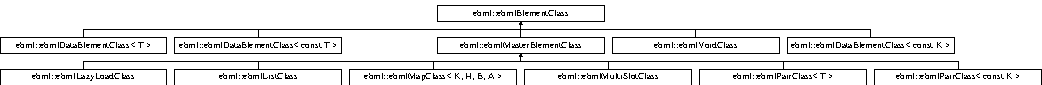
\includegraphics[height=1.138211cm]{classebml_1_1ebmlElementClass}
\end{center}
\end{figure}
\subsection*{Public Member Functions}
\begin{DoxyCompactItemize}
\item 
\mbox{\hyperlink{classebml_1_1ebmlElementClass_a6c2081870c5d66c70e0cf988ff253420}{ebml\+Element\+Class}} (const char $\ast$\mbox{\hyperlink{classebml_1_1ebmlElementClass_a7d8337c9f9b884b43e1618b9392519b6}{ebml\+ID}}, const std\+::wstring \&\mbox{\hyperlink{classebml_1_1ebmlElementClass_aba4096c056179fb989da05d86f4cb46d}{name}})
\item 
\mbox{\hyperlink{classebml_1_1ebmlElementClass_a9ea21779aa5db15a70df73a03a873aa8}{ebml\+Element\+Class}} (\mbox{\hyperlink{namespaceebml_a86c5f604ddf12a74aa9812e997a58691}{ebml\+I\+D\+\_\+t}} \mbox{\hyperlink{classebml_1_1ebmlElementClass_a7d8337c9f9b884b43e1618b9392519b6}{ebml\+ID}}, const std\+::wstring \&\mbox{\hyperlink{classebml_1_1ebmlElementClass_aba4096c056179fb989da05d86f4cb46d}{name}})
\item 
\mbox{\hyperlink{namespaceebml_adad533b7705a16bb360fe56380c5e7be}{ebml\+Element\+\_\+sp}} \mbox{\hyperlink{classebml_1_1ebmlElementClass_a45bdca04f3008152ad7df0856ef8724b}{operator()}} () const
\item 
\mbox{\hyperlink{namespaceebml_adad533b7705a16bb360fe56380c5e7be}{ebml\+Element\+\_\+sp}} \mbox{\hyperlink{classebml_1_1ebmlElementClass_a9de19726c4794e4e3cb1f32e445c5002}{decode}} (const \mbox{\hyperlink{classebml_1_1parseString}{parse\+String}} \&) const
\item 
virtual \mbox{\hyperlink{namespaceebml_adad533b7705a16bb360fe56380c5e7be}{ebml\+Element\+\_\+sp}} \mbox{\hyperlink{classebml_1_1ebmlElementClass_aa6bf675de4918fd7b553d141871a2ede}{\+\_\+decode}} (const \mbox{\hyperlink{classebml_1_1parseString}{parse\+String}} \&) const =0
\item 
\mbox{\hyperlink{namespaceebml_adad533b7705a16bb360fe56380c5e7be}{ebml\+Element\+\_\+sp}} \mbox{\hyperlink{classebml_1_1ebmlElementClass_ab7f46d2ffffadf3b8be8f1d780b15a41}{decode}} (const \mbox{\hyperlink{classebml_1_1parseFile}{parse\+File}} \&) const
\item 
virtual \mbox{\hyperlink{namespaceebml_adad533b7705a16bb360fe56380c5e7be}{ebml\+Element\+\_\+sp}} \mbox{\hyperlink{classebml_1_1ebmlElementClass_aedbfff5909af215acaa3ca28643f1bc9}{\+\_\+decode}} (const \mbox{\hyperlink{classebml_1_1parseFile}{parse\+File}} \&) const =0
\item 
\mbox{\hyperlink{namespaceebml_adad533b7705a16bb360fe56380c5e7be}{ebml\+Element\+\_\+sp}} \mbox{\hyperlink{classebml_1_1ebmlElementClass_ac24711e997db80f691a8bff4f610242f}{decode}} (const char $\ast$\mbox{\hyperlink{namespaceebml_ab21f8b4ff85186f670f17e84a02d9740}{data}}, size\+\_\+t \mbox{\hyperlink{namespaceebml_a75eaf24de9c90584c60e27de3b1dd63e}{size}}) const
\item 
\mbox{\hyperlink{namespaceebml_adad533b7705a16bb360fe56380c5e7be}{ebml\+Element\+\_\+sp}} \mbox{\hyperlink{classebml_1_1ebmlElementClass_a2e45d73cfc2bfda5b4731af42299aaf1}{decode}} (const std\+::string \&\mbox{\hyperlink{namespaceebml_ab21f8b4ff85186f670f17e84a02d9740}{data}}) const
\item 
\mbox{\hyperlink{namespaceebml_adad533b7705a16bb360fe56380c5e7be}{ebml\+Element\+\_\+sp}} \mbox{\hyperlink{classebml_1_1ebmlElementClass_ade81fc2a088d16f40474fd9885770f84}{decode}} (\mbox{\hyperlink{namespaceebml_a7bb59128ac6af27e47367938a846b569}{io\+Base\+\_\+sp}} \&) const
\item 
\mbox{\hyperlink{namespaceebml_adad533b7705a16bb360fe56380c5e7be}{ebml\+Element\+\_\+sp}} \mbox{\hyperlink{classebml_1_1ebmlElementClass_a313f310d2501859a73ba5d19ebacb550}{decode}} (\mbox{\hyperlink{classebml_1_1ioBase}{io\+Base}} $\ast$) const
\item 
\mbox{\hyperlink{namespaceebml_adad533b7705a16bb360fe56380c5e7be}{ebml\+Element\+\_\+sp}} \mbox{\hyperlink{classebml_1_1ebmlElementClass_a22d53b2eb309a030d1e4691bd564d08e}{decode}} (\mbox{\hyperlink{namespaceebml_a7bb59128ac6af27e47367938a846b569}{io\+Base\+\_\+sp}} \&, off\+\_\+t \&) const
\item 
\mbox{\hyperlink{namespaceebml_adad533b7705a16bb360fe56380c5e7be}{ebml\+Element\+\_\+sp}} \mbox{\hyperlink{classebml_1_1ebmlElementClass_a4441b1ac041896cf7bccd9d59ebbf080}{decode}} (\mbox{\hyperlink{classebml_1_1ioBase}{io\+Base}} $\ast$, off\+\_\+t \&) const
\item 
\mbox{\hyperlink{namespaceebml_adad533b7705a16bb360fe56380c5e7be}{ebml\+Element\+\_\+sp}} \mbox{\hyperlink{classebml_1_1ebmlElementClass_ae7d79a92abd19825137ccb0b7d1893e7}{decode}} (\mbox{\hyperlink{namespaceebml_a7bb59128ac6af27e47367938a846b569}{io\+Base\+\_\+sp}} \&, off\+\_\+t, off\+\_\+t \&) const
\item 
\mbox{\hyperlink{namespaceebml_adad533b7705a16bb360fe56380c5e7be}{ebml\+Element\+\_\+sp}} \mbox{\hyperlink{classebml_1_1ebmlElementClass_a7c8b6853b84adff619ba8700070a9997}{decode}} (\mbox{\hyperlink{classebml_1_1ioBase}{io\+Base}} $\ast$, off\+\_\+t, off\+\_\+t \&) const
\item 
\mbox{\hyperlink{namespaceebml_a2deef4e8071531b32e3533f1bf978917}{c\+\_\+ebml\+Element\+\_\+sp}} \mbox{\hyperlink{classebml_1_1ebmlElementClass_ad44d7844db705e5e1d8c35a780b58486}{cdecode}} (const \mbox{\hyperlink{classebml_1_1parseString}{parse\+String}} \&) const
\item 
\mbox{\hyperlink{namespaceebml_a2deef4e8071531b32e3533f1bf978917}{c\+\_\+ebml\+Element\+\_\+sp}} \mbox{\hyperlink{classebml_1_1ebmlElementClass_a6a6432b7bf633821f27015e111928b15}{cdecode}} (const \mbox{\hyperlink{classebml_1_1parseFile}{parse\+File}} \&) const
\item 
\mbox{\hyperlink{namespaceebml_a2deef4e8071531b32e3533f1bf978917}{c\+\_\+ebml\+Element\+\_\+sp}} \mbox{\hyperlink{classebml_1_1ebmlElementClass_ab365b1b7024bbf0dd625694a71f7e7ba}{cdecode}} (const char $\ast$, size\+\_\+t) const
\item 
\mbox{\hyperlink{namespaceebml_a2deef4e8071531b32e3533f1bf978917}{c\+\_\+ebml\+Element\+\_\+sp}} \mbox{\hyperlink{classebml_1_1ebmlElementClass_a2696f361d3cf6f1f544657266ad21808}{cdecode}} (const std\+::string \&) const
\item 
\mbox{\hyperlink{namespaceebml_a2deef4e8071531b32e3533f1bf978917}{c\+\_\+ebml\+Element\+\_\+sp}} \mbox{\hyperlink{classebml_1_1ebmlElementClass_a01de47338b3df5a666b989d9d85fa1d5}{cdecode}} (\mbox{\hyperlink{namespaceebml_a7bb59128ac6af27e47367938a846b569}{io\+Base\+\_\+sp}} \&) const
\item 
\mbox{\hyperlink{namespaceebml_a2deef4e8071531b32e3533f1bf978917}{c\+\_\+ebml\+Element\+\_\+sp}} \mbox{\hyperlink{classebml_1_1ebmlElementClass_a583586c72ae328913f0a920843d46677}{cdecode}} (\mbox{\hyperlink{classebml_1_1ioBase}{io\+Base}} $\ast$) const
\item 
virtual \mbox{\hyperlink{classebml_1_1seekData__t}{seek\+Data\+\_\+t}} $\ast$ \mbox{\hyperlink{classebml_1_1ebmlElementClass_a211de9c10948a2b4a6b3550eb76c1102}{make\+Seek\+Data}} (const \mbox{\hyperlink{classebml_1_1parseFile}{parse\+File}} \&) const
\item 
virtual \mbox{\hyperlink{classebml_1_1seekData__t}{seek\+Data\+\_\+t}} $\ast$ \mbox{\hyperlink{classebml_1_1ebmlElementClass_ac844edef1226b728c127cdf946b3d152}{make\+Seek\+Data}} (const \mbox{\hyperlink{classebml_1_1parseFile}{parse\+File}} \&, const \mbox{\hyperlink{namespaceebml_adad533b7705a16bb360fe56380c5e7be}{ebml\+Element\+\_\+sp}} \&) const
\item 
{\footnotesize template$<$typename T  = ebml\+Element\+Class$>$ }\\T \& \mbox{\hyperlink{classebml_1_1ebmlElementClass_ab8c68b1f0a25aead5003d7100a27d5d3}{as}} ()
\item 
{\footnotesize template$<$typename T  = ebml\+Element\+Class$>$ }\\const T \& \mbox{\hyperlink{classebml_1_1ebmlElementClass_a5d49c645d8b92ef330e5960a02f2fbf7}{as}} () const
\item 
{\footnotesize template$<$typename T  = ebml\+Element\+Class$>$ }\\T $\ast$ \mbox{\hyperlink{classebml_1_1ebmlElementClass_a485c3f4a11b09d301b80f44e1802e9ab}{ptr}} ()
\item 
{\footnotesize template$<$typename T  = ebml\+Element\+Class$>$ }\\const T $\ast$ \mbox{\hyperlink{classebml_1_1ebmlElementClass_a4d3188e97ab01f1db0427faa5b5d6059}{ptr}} () const
\item 
virtual std\+::wstring \mbox{\hyperlink{classebml_1_1ebmlElementClass_a251cc751901423a86099d58d49f28291}{minirepr}} () const
\item 
std\+::wstring \mbox{\hyperlink{classebml_1_1ebmlElementClass_a117d6f78c2bdaa4dbf02cab30510d8f5}{repr}} () const
\end{DoxyCompactItemize}
\subsection*{Public Attributes}
\begin{DoxyCompactItemize}
\item 
\mbox{\hyperlink{namespaceebml_a86c5f604ddf12a74aa9812e997a58691}{ebml\+I\+D\+\_\+t}} \mbox{\hyperlink{classebml_1_1ebmlElementClass_a7d8337c9f9b884b43e1618b9392519b6}{ebml\+ID}}
\item 
std\+::wstring \mbox{\hyperlink{classebml_1_1ebmlElementClass_aba4096c056179fb989da05d86f4cb46d}{name}}
\end{DoxyCompactItemize}
\subsection*{Protected Member Functions}
\begin{DoxyCompactItemize}
\item 
virtual \mbox{\hyperlink{classebml_1_1ebmlElement}{ebml\+Element}} $\ast$ \mbox{\hyperlink{classebml_1_1ebmlElementClass_a223ede6b8bc3c85251d2d73f0256fb45}{\+\_\+new}} () const =0
\item 
virtual \mbox{\hyperlink{namespaceebml_adad533b7705a16bb360fe56380c5e7be}{ebml\+Element\+\_\+sp}} \mbox{\hyperlink{classebml_1_1ebmlElementClass_a81f0713cca953599d74185aa24c4c2c1}{\+\_\+cdecode}} (const \mbox{\hyperlink{classebml_1_1parseString}{parse\+String}} \&) const
\item 
virtual \mbox{\hyperlink{namespaceebml_adad533b7705a16bb360fe56380c5e7be}{ebml\+Element\+\_\+sp}} \mbox{\hyperlink{classebml_1_1ebmlElementClass_ae423476637d4ca052cd7aa0047f2b3eb}{\+\_\+cdecode}} (const \mbox{\hyperlink{classebml_1_1parseFile}{parse\+File}} \&) const
\end{DoxyCompactItemize}
\subsection*{Friends}
\begin{DoxyCompactItemize}
\item 
class \mbox{\hyperlink{classebml_1_1ebmlElementClass_ab57be41c560fe3aac8d5eb6b138c09a5}{ebml\+Element}}
\item 
class \mbox{\hyperlink{classebml_1_1ebmlElementClass_ad88e86cba72e9332a4693c1c6009b281}{ebml\+Master\+Element}}
\item 
class \mbox{\hyperlink{classebml_1_1ebmlElementClass_aa005a2a7ef20ef779d383e3da2e0b46d}{ebml\+Master\+Element\+Class}}
\end{DoxyCompactItemize}


\subsection{Detailed Description}
Abstract base class for E\+B\+ML Element Type objects. Every subclass of \mbox{\hyperlink{classebml_1_1ebmlElementClass}{ebml\+Element\+Class}} must have a companion subclass of \mbox{\hyperlink{classebml_1_1ebmlElement}{ebml\+Element}} declared as a friend class.

Instances of \mbox{\hyperlink{classebml_1_1ebmlElementClass}{ebml\+Element\+Class}} are constructed using an E\+B\+ML ID, either as an ebml\+I\+D\+\_\+t (unsigned long long) or as a V\+I\+NT (const char$\ast$), and a class name (unicode string). 

\subsection{Constructor \& Destructor Documentation}
\mbox{\Hypertarget{classebml_1_1ebmlElementClass_a6c2081870c5d66c70e0cf988ff253420}\label{classebml_1_1ebmlElementClass_a6c2081870c5d66c70e0cf988ff253420}} 
\index{ebml\+::ebml\+Element\+Class@{ebml\+::ebml\+Element\+Class}!ebml\+Element\+Class@{ebml\+Element\+Class}}
\index{ebml\+Element\+Class@{ebml\+Element\+Class}!ebml\+::ebml\+Element\+Class@{ebml\+::ebml\+Element\+Class}}
\subsubsection{\texorpdfstring{ebml\+Element\+Class()}{ebmlElementClass()}\hspace{0.1cm}{\footnotesize\ttfamily [1/2]}}
{\footnotesize\ttfamily ebml\+::ebml\+Element\+Class\+::ebml\+Element\+Class (\begin{DoxyParamCaption}\item[{const char $\ast$}]{ebml\+ID,  }\item[{const std\+::wstring \&}]{name }\end{DoxyParamCaption})}

Constructor for E\+B\+ML Element Type objects.


\begin{DoxyParams}{Parameters}
{\em ebml\+ID} & E\+B\+ML ID as a V\+I\+NT string. \\
\hline
{\em name} & Name for E\+B\+ML Element Type.\\
\hline
\end{DoxyParams}
Example\+: 
\begin{DoxyCode}
\mbox{\hyperlink{classebml_1_1ebmlVoidClass_afc8666d6bbcd41bad76bfc5a2b5b4c9a}{ebmlVoidClass::ebmlVoidClass}}() : \mbox{\hyperlink{classebml_1_1ebmlElementClass_a6c2081870c5d66c70e0cf988ff253420}{ebmlElementClass}}(\textcolor{stringliteral}{"\(\backslash\)xec"}, \textcolor{stringliteral}{"
      EBMLVoid"}) \{\}
\end{DoxyCode}
 \mbox{\Hypertarget{classebml_1_1ebmlElementClass_a9ea21779aa5db15a70df73a03a873aa8}\label{classebml_1_1ebmlElementClass_a9ea21779aa5db15a70df73a03a873aa8}} 
\index{ebml\+::ebml\+Element\+Class@{ebml\+::ebml\+Element\+Class}!ebml\+Element\+Class@{ebml\+Element\+Class}}
\index{ebml\+Element\+Class@{ebml\+Element\+Class}!ebml\+::ebml\+Element\+Class@{ebml\+::ebml\+Element\+Class}}
\subsubsection{\texorpdfstring{ebml\+Element\+Class()}{ebmlElementClass()}\hspace{0.1cm}{\footnotesize\ttfamily [2/2]}}
{\footnotesize\ttfamily ebml\+::ebml\+Element\+Class\+::ebml\+Element\+Class (\begin{DoxyParamCaption}\item[{\mbox{\hyperlink{namespaceebml_a86c5f604ddf12a74aa9812e997a58691}{ebml\+I\+D\+\_\+t}}}]{ebml\+ID,  }\item[{const std\+::wstring \&}]{name }\end{DoxyParamCaption})}

Constructor for E\+B\+ML Element Type objects.


\begin{DoxyParams}{Parameters}
{\em ebml\+ID} & E\+B\+ML ID as an unsigned integer. \\
\hline
{\em name} & Name for E\+B\+ML Element Type.\\
\hline
\end{DoxyParams}
Example\+: 
\begin{DoxyCode}
\mbox{\hyperlink{classebml_1_1ebmlVoidClass_afc8666d6bbcd41bad76bfc5a2b5b4c9a}{ebmlVoidClass::ebmlVoidClass}}() : \mbox{\hyperlink{classebml_1_1ebmlElementClass_a6c2081870c5d66c70e0cf988ff253420}{ebmlElementClass}}(108, \textcolor{stringliteral}{"
      EBMLVoid"}) \{\}
\end{DoxyCode}
 

\subsection{Member Function Documentation}
\mbox{\Hypertarget{classebml_1_1ebmlElementClass_a81f0713cca953599d74185aa24c4c2c1}\label{classebml_1_1ebmlElementClass_a81f0713cca953599d74185aa24c4c2c1}} 
\index{ebml\+::ebml\+Element\+Class@{ebml\+::ebml\+Element\+Class}!\+\_\+cdecode@{\+\_\+cdecode}}
\index{\+\_\+cdecode@{\+\_\+cdecode}!ebml\+::ebml\+Element\+Class@{ebml\+::ebml\+Element\+Class}}
\subsubsection{\texorpdfstring{\+\_\+cdecode()}{\_cdecode()}\hspace{0.1cm}{\footnotesize\ttfamily [1/2]}}
{\footnotesize\ttfamily virtual \mbox{\hyperlink{namespaceebml_adad533b7705a16bb360fe56380c5e7be}{ebml\+Element\+\_\+sp}} ebml\+::ebml\+Element\+Class\+::\+\_\+cdecode (\begin{DoxyParamCaption}\item[{const \mbox{\hyperlink{classebml_1_1parseString}{parse\+String}} \&}]{ }\end{DoxyParamCaption}) const\hspace{0.3cm}{\ttfamily [protected]}, {\ttfamily [virtual]}}



Reimplemented in \mbox{\hyperlink{classebml_1_1ebmlMasterElementClass_a8b57f2fe211ab7a418f8b7d4a981a1d7}{ebml\+::ebml\+Master\+Element\+Class}}.

\mbox{\Hypertarget{classebml_1_1ebmlElementClass_ae423476637d4ca052cd7aa0047f2b3eb}\label{classebml_1_1ebmlElementClass_ae423476637d4ca052cd7aa0047f2b3eb}} 
\index{ebml\+::ebml\+Element\+Class@{ebml\+::ebml\+Element\+Class}!\+\_\+cdecode@{\+\_\+cdecode}}
\index{\+\_\+cdecode@{\+\_\+cdecode}!ebml\+::ebml\+Element\+Class@{ebml\+::ebml\+Element\+Class}}
\subsubsection{\texorpdfstring{\+\_\+cdecode()}{\_cdecode()}\hspace{0.1cm}{\footnotesize\ttfamily [2/2]}}
{\footnotesize\ttfamily virtual \mbox{\hyperlink{namespaceebml_adad533b7705a16bb360fe56380c5e7be}{ebml\+Element\+\_\+sp}} ebml\+::ebml\+Element\+Class\+::\+\_\+cdecode (\begin{DoxyParamCaption}\item[{const \mbox{\hyperlink{classebml_1_1parseFile}{parse\+File}} \&}]{ }\end{DoxyParamCaption}) const\hspace{0.3cm}{\ttfamily [protected]}, {\ttfamily [virtual]}}



Reimplemented in \mbox{\hyperlink{classebml_1_1ebmlMasterElementClass_a6ef689ac153338400cfb8367edd32f54}{ebml\+::ebml\+Master\+Element\+Class}}.

\mbox{\Hypertarget{classebml_1_1ebmlElementClass_aa6bf675de4918fd7b553d141871a2ede}\label{classebml_1_1ebmlElementClass_aa6bf675de4918fd7b553d141871a2ede}} 
\index{ebml\+::ebml\+Element\+Class@{ebml\+::ebml\+Element\+Class}!\+\_\+decode@{\+\_\+decode}}
\index{\+\_\+decode@{\+\_\+decode}!ebml\+::ebml\+Element\+Class@{ebml\+::ebml\+Element\+Class}}
\subsubsection{\texorpdfstring{\+\_\+decode()}{\_decode()}\hspace{0.1cm}{\footnotesize\ttfamily [1/2]}}
{\footnotesize\ttfamily virtual \mbox{\hyperlink{namespaceebml_adad533b7705a16bb360fe56380c5e7be}{ebml\+Element\+\_\+sp}} ebml\+::ebml\+Element\+Class\+::\+\_\+decode (\begin{DoxyParamCaption}\item[{const \mbox{\hyperlink{classebml_1_1parseString}{parse\+String}} \&}]{ }\end{DoxyParamCaption}) const\hspace{0.3cm}{\ttfamily [pure virtual]}}



Implemented in \mbox{\hyperlink{classebml_1_1ebmlMasterElementClass_a4499f7187f0480518080cf8135884981}{ebml\+::ebml\+Master\+Element\+Class}}, \mbox{\hyperlink{classebml_1_1ebmlDataElementClass_3_01const_01T_01_4_a0f8a6e30cd3cc630950a780a726849a7}{ebml\+::ebml\+Data\+Element\+Class$<$ const T $>$}}, \mbox{\hyperlink{classebml_1_1ebmlDataElementClass_a481cda6ab9f96ab21434daabd9ad1ed9}{ebml\+::ebml\+Data\+Element\+Class$<$ T $>$}}, \mbox{\hyperlink{classebml_1_1ebmlDataElementClass_a481cda6ab9f96ab21434daabd9ad1ed9}{ebml\+::ebml\+Data\+Element\+Class$<$ const K $>$}}, and \mbox{\hyperlink{classebml_1_1ebmlVoidClass_ab12dc43d26e82dee3c66d69219e4d78d}{ebml\+::ebml\+Void\+Class}}.

\mbox{\Hypertarget{classebml_1_1ebmlElementClass_aedbfff5909af215acaa3ca28643f1bc9}\label{classebml_1_1ebmlElementClass_aedbfff5909af215acaa3ca28643f1bc9}} 
\index{ebml\+::ebml\+Element\+Class@{ebml\+::ebml\+Element\+Class}!\+\_\+decode@{\+\_\+decode}}
\index{\+\_\+decode@{\+\_\+decode}!ebml\+::ebml\+Element\+Class@{ebml\+::ebml\+Element\+Class}}
\subsubsection{\texorpdfstring{\+\_\+decode()}{\_decode()}\hspace{0.1cm}{\footnotesize\ttfamily [2/2]}}
{\footnotesize\ttfamily virtual \mbox{\hyperlink{namespaceebml_adad533b7705a16bb360fe56380c5e7be}{ebml\+Element\+\_\+sp}} ebml\+::ebml\+Element\+Class\+::\+\_\+decode (\begin{DoxyParamCaption}\item[{const \mbox{\hyperlink{classebml_1_1parseFile}{parse\+File}} \&}]{ }\end{DoxyParamCaption}) const\hspace{0.3cm}{\ttfamily [pure virtual]}}



Implemented in \mbox{\hyperlink{classebml_1_1ebmlMasterElementClass_aeda43063d78233403fa084800ff9c109}{ebml\+::ebml\+Master\+Element\+Class}}, \mbox{\hyperlink{classebml_1_1ebmlDataElementClass_3_01const_01T_01_4_a472912867198ebff97d963cdd7f5ce33}{ebml\+::ebml\+Data\+Element\+Class$<$ const T $>$}}, \mbox{\hyperlink{classebml_1_1ebmlDataElementClass_ac0b070ab767aecb9387f9c0e412e8136}{ebml\+::ebml\+Data\+Element\+Class$<$ T $>$}}, \mbox{\hyperlink{classebml_1_1ebmlDataElementClass_ac0b070ab767aecb9387f9c0e412e8136}{ebml\+::ebml\+Data\+Element\+Class$<$ const K $>$}}, and \mbox{\hyperlink{classebml_1_1ebmlVoidClass_a4b4b65f2289a5f4cbd182dac7b5aa1db}{ebml\+::ebml\+Void\+Class}}.

\mbox{\Hypertarget{classebml_1_1ebmlElementClass_a223ede6b8bc3c85251d2d73f0256fb45}\label{classebml_1_1ebmlElementClass_a223ede6b8bc3c85251d2d73f0256fb45}} 
\index{ebml\+::ebml\+Element\+Class@{ebml\+::ebml\+Element\+Class}!\+\_\+new@{\+\_\+new}}
\index{\+\_\+new@{\+\_\+new}!ebml\+::ebml\+Element\+Class@{ebml\+::ebml\+Element\+Class}}
\subsubsection{\texorpdfstring{\+\_\+new()}{\_new()}}
{\footnotesize\ttfamily virtual \mbox{\hyperlink{classebml_1_1ebmlElement}{ebml\+Element}}$\ast$ ebml\+::ebml\+Element\+Class\+::\+\_\+new (\begin{DoxyParamCaption}{ }\end{DoxyParamCaption}) const\hspace{0.3cm}{\ttfamily [protected]}, {\ttfamily [pure virtual]}}



Implemented in \mbox{\hyperlink{classebml_1_1ebmlMapClass_a3370b9b3457982693c08723af7d5130a}{ebml\+::ebml\+Map\+Class$<$ K, H, E, A $>$}}, \mbox{\hyperlink{classebml_1_1ebmlDataElementClass_3_01const_01T_01_4_aaf6b66092e1987919e277661b62f2d90}{ebml\+::ebml\+Data\+Element\+Class$<$ const T $>$}}, \mbox{\hyperlink{classebml_1_1ebmlMultiSlotClass_ab0cb2ed53ef6a3a8e64ffc47c72f5b94}{ebml\+::ebml\+Multi\+Slot\+Class}}, \mbox{\hyperlink{classebml_1_1ebmlPairClass_abb748027028719a4a1682c089ac21226}{ebml\+::ebml\+Pair\+Class$<$ T $>$}}, \mbox{\hyperlink{classebml_1_1ebmlPairClass_abb748027028719a4a1682c089ac21226}{ebml\+::ebml\+Pair\+Class$<$ const K $>$}}, \mbox{\hyperlink{classebml_1_1ebmlLazyLoadClass_a5492f081f425fcbff11095f483b52f32}{ebml\+::ebml\+Lazy\+Load\+Class}}, \mbox{\hyperlink{classebml_1_1ebmlDataElementClass_a79fabffdfd33bee94cd14416646da546}{ebml\+::ebml\+Data\+Element\+Class$<$ T $>$}}, \mbox{\hyperlink{classebml_1_1ebmlDataElementClass_a79fabffdfd33bee94cd14416646da546}{ebml\+::ebml\+Data\+Element\+Class$<$ const K $>$}}, \mbox{\hyperlink{classebml_1_1ebmlListClass_aef729ee70f218de1013c3782c481bffb}{ebml\+::ebml\+List\+Class}}, and \mbox{\hyperlink{classebml_1_1ebmlVoidClass_a3403a8145594a3ce5e34b02dd2f938ae}{ebml\+::ebml\+Void\+Class}}.

\mbox{\Hypertarget{classebml_1_1ebmlElementClass_ab8c68b1f0a25aead5003d7100a27d5d3}\label{classebml_1_1ebmlElementClass_ab8c68b1f0a25aead5003d7100a27d5d3}} 
\index{ebml\+::ebml\+Element\+Class@{ebml\+::ebml\+Element\+Class}!as@{as}}
\index{as@{as}!ebml\+::ebml\+Element\+Class@{ebml\+::ebml\+Element\+Class}}
\subsubsection{\texorpdfstring{as()}{as()}\hspace{0.1cm}{\footnotesize\ttfamily [1/2]}}
{\footnotesize\ttfamily template$<$typename T  = ebml\+Element\+Class$>$ \\
T\& ebml\+::ebml\+Element\+Class\+::as (\begin{DoxyParamCaption}{ }\end{DoxyParamCaption})\hspace{0.3cm}{\ttfamily [inline]}}

Convenience member function that dynamically casts \mbox{\hyperlink{classebml_1_1ebmlElementClass}{ebml\+Element\+Class}} to a subclass.

\begin{DoxyReturn}{Returns}
Reference to instance as a T object.
\end{DoxyReturn}
Example\+: 
\begin{DoxyCode}
\mbox{\hyperlink{classebml_1_1ebmlElementClass_a6c2081870c5d66c70e0cf988ff253420}{ebmlElementClass}} \mbox{\hyperlink{classebml_1_1ebmlElement_a15cf59e94b01e2c49ec96512b9bd9d90}{cls}} = ebmlVoidClass();
ebmlVoidClass& \mbox{\hyperlink{namespaceebml_afbfd509d1cb71e416a07253746e886e9}{Void}} = \mbox{\hyperlink{classebml_1_1ebmlElement_a15cf59e94b01e2c49ec96512b9bd9d90}{cls}}.ref<ebmlVoidClass>();
\end{DoxyCode}
 
\begin{DoxyExceptions}{Exceptions}
{\em std\+::bad\+\_\+alloc} & If instance is not an instance of T. \\
\hline
\end{DoxyExceptions}
\mbox{\Hypertarget{classebml_1_1ebmlElementClass_a5d49c645d8b92ef330e5960a02f2fbf7}\label{classebml_1_1ebmlElementClass_a5d49c645d8b92ef330e5960a02f2fbf7}} 
\index{ebml\+::ebml\+Element\+Class@{ebml\+::ebml\+Element\+Class}!as@{as}}
\index{as@{as}!ebml\+::ebml\+Element\+Class@{ebml\+::ebml\+Element\+Class}}
\subsubsection{\texorpdfstring{as()}{as()}\hspace{0.1cm}{\footnotesize\ttfamily [2/2]}}
{\footnotesize\ttfamily template$<$typename T  = ebml\+Element\+Class$>$ \\
const T\& ebml\+::ebml\+Element\+Class\+::as (\begin{DoxyParamCaption}{ }\end{DoxyParamCaption}) const\hspace{0.3cm}{\ttfamily [inline]}}

Convenience member function that dynamically casts const \mbox{\hyperlink{classebml_1_1ebmlElementClass}{ebml\+Element\+Class}} to a subclass.

\begin{DoxyReturn}{Returns}
Const reference to instance as a T object.
\end{DoxyReturn}
Example\+: 
\begin{DoxyCode}
\textcolor{keyword}{const} \mbox{\hyperlink{classebml_1_1ebmlElementClass_a6c2081870c5d66c70e0cf988ff253420}{ebmlElementClass}} \mbox{\hyperlink{classebml_1_1ebmlElement_a15cf59e94b01e2c49ec96512b9bd9d90}{cls}} = ebmlVoidClass();
\textcolor{keyword}{const} ebmlVoidClass& \mbox{\hyperlink{namespaceebml_afbfd509d1cb71e416a07253746e886e9}{Void}} = \mbox{\hyperlink{classebml_1_1ebmlElement_a15cf59e94b01e2c49ec96512b9bd9d90}{cls}}.a<ebmlVoidClass>();
\end{DoxyCode}
 
\begin{DoxyExceptions}{Exceptions}
{\em std\+::bad\+\_\+alloc} & If instance is not an instance of T. \\
\hline
\end{DoxyExceptions}
\mbox{\Hypertarget{classebml_1_1ebmlElementClass_ad44d7844db705e5e1d8c35a780b58486}\label{classebml_1_1ebmlElementClass_ad44d7844db705e5e1d8c35a780b58486}} 
\index{ebml\+::ebml\+Element\+Class@{ebml\+::ebml\+Element\+Class}!cdecode@{cdecode}}
\index{cdecode@{cdecode}!ebml\+::ebml\+Element\+Class@{ebml\+::ebml\+Element\+Class}}
\subsubsection{\texorpdfstring{cdecode()}{cdecode()}\hspace{0.1cm}{\footnotesize\ttfamily [1/6]}}
{\footnotesize\ttfamily \mbox{\hyperlink{namespaceebml_a2deef4e8071531b32e3533f1bf978917}{c\+\_\+ebml\+Element\+\_\+sp}} ebml\+::ebml\+Element\+Class\+::cdecode (\begin{DoxyParamCaption}\item[{const \mbox{\hyperlink{classebml_1_1parseString}{parse\+String}} \&}]{ }\end{DoxyParamCaption}) const}

\mbox{\Hypertarget{classebml_1_1ebmlElementClass_a6a6432b7bf633821f27015e111928b15}\label{classebml_1_1ebmlElementClass_a6a6432b7bf633821f27015e111928b15}} 
\index{ebml\+::ebml\+Element\+Class@{ebml\+::ebml\+Element\+Class}!cdecode@{cdecode}}
\index{cdecode@{cdecode}!ebml\+::ebml\+Element\+Class@{ebml\+::ebml\+Element\+Class}}
\subsubsection{\texorpdfstring{cdecode()}{cdecode()}\hspace{0.1cm}{\footnotesize\ttfamily [2/6]}}
{\footnotesize\ttfamily \mbox{\hyperlink{namespaceebml_a2deef4e8071531b32e3533f1bf978917}{c\+\_\+ebml\+Element\+\_\+sp}} ebml\+::ebml\+Element\+Class\+::cdecode (\begin{DoxyParamCaption}\item[{const \mbox{\hyperlink{classebml_1_1parseFile}{parse\+File}} \&}]{ }\end{DoxyParamCaption}) const}

\mbox{\Hypertarget{classebml_1_1ebmlElementClass_ab365b1b7024bbf0dd625694a71f7e7ba}\label{classebml_1_1ebmlElementClass_ab365b1b7024bbf0dd625694a71f7e7ba}} 
\index{ebml\+::ebml\+Element\+Class@{ebml\+::ebml\+Element\+Class}!cdecode@{cdecode}}
\index{cdecode@{cdecode}!ebml\+::ebml\+Element\+Class@{ebml\+::ebml\+Element\+Class}}
\subsubsection{\texorpdfstring{cdecode()}{cdecode()}\hspace{0.1cm}{\footnotesize\ttfamily [3/6]}}
{\footnotesize\ttfamily \mbox{\hyperlink{namespaceebml_a2deef4e8071531b32e3533f1bf978917}{c\+\_\+ebml\+Element\+\_\+sp}} ebml\+::ebml\+Element\+Class\+::cdecode (\begin{DoxyParamCaption}\item[{const char $\ast$}]{,  }\item[{size\+\_\+t}]{ }\end{DoxyParamCaption}) const}

Create const \mbox{\hyperlink{classebml_1_1ebmlElement}{ebml\+Element}} instance, decoding from a const char$\ast$ array.


\begin{DoxyParams}{Parameters}
{\em data} & Data to decode. \\
\hline
{\em size} & Size of \textquotesingle{}data\textquotesingle{}. \\
\hline
\end{DoxyParams}
\begin{DoxyReturn}{Returns}
Shared pointer to new \mbox{\hyperlink{classebml_1_1ebmlElement}{ebml\+Element}} instance.
\end{DoxyReturn}
Example\+: 
\begin{DoxyCode}
ebmlVoidClass \mbox{\hyperlink{namespaceebml_afbfd509d1cb71e416a07253746e886e9}{Void}};
\textcolor{keyword}{const} \textcolor{keywordtype}{char}* = \textcolor{stringliteral}{"\(\backslash\)xec\(\backslash\)x82\(\backslash\)x00\(\backslash\)x00"};
\mbox{\hyperlink{namespaceebml_adad533b7705a16bb360fe56380c5e7be}{ebmlElement\_sp}} elem = \mbox{\hyperlink{namespaceebml_afbfd509d1cb71e416a07253746e886e9}{Void}}.\mbox{\hyperlink{classebml_1_1ebmlElementClass_ad44d7844db705e5e1d8c35a780b58486}{cdecode}}(\mbox{\hyperlink{namespaceebml_ab21f8b4ff85186f670f17e84a02d9740}{data}}, 4);
\end{DoxyCode}
 \mbox{\Hypertarget{classebml_1_1ebmlElementClass_a2696f361d3cf6f1f544657266ad21808}\label{classebml_1_1ebmlElementClass_a2696f361d3cf6f1f544657266ad21808}} 
\index{ebml\+::ebml\+Element\+Class@{ebml\+::ebml\+Element\+Class}!cdecode@{cdecode}}
\index{cdecode@{cdecode}!ebml\+::ebml\+Element\+Class@{ebml\+::ebml\+Element\+Class}}
\subsubsection{\texorpdfstring{cdecode()}{cdecode()}\hspace{0.1cm}{\footnotesize\ttfamily [4/6]}}
{\footnotesize\ttfamily \mbox{\hyperlink{namespaceebml_a2deef4e8071531b32e3533f1bf978917}{c\+\_\+ebml\+Element\+\_\+sp}} ebml\+::ebml\+Element\+Class\+::cdecode (\begin{DoxyParamCaption}\item[{const std\+::string \&}]{ }\end{DoxyParamCaption}) const}

\mbox{\Hypertarget{classebml_1_1ebmlElementClass_a01de47338b3df5a666b989d9d85fa1d5}\label{classebml_1_1ebmlElementClass_a01de47338b3df5a666b989d9d85fa1d5}} 
\index{ebml\+::ebml\+Element\+Class@{ebml\+::ebml\+Element\+Class}!cdecode@{cdecode}}
\index{cdecode@{cdecode}!ebml\+::ebml\+Element\+Class@{ebml\+::ebml\+Element\+Class}}
\subsubsection{\texorpdfstring{cdecode()}{cdecode()}\hspace{0.1cm}{\footnotesize\ttfamily [5/6]}}
{\footnotesize\ttfamily \mbox{\hyperlink{namespaceebml_a2deef4e8071531b32e3533f1bf978917}{c\+\_\+ebml\+Element\+\_\+sp}} ebml\+::ebml\+Element\+Class\+::cdecode (\begin{DoxyParamCaption}\item[{\mbox{\hyperlink{namespaceebml_a7bb59128ac6af27e47367938a846b569}{io\+Base\+\_\+sp}} \&}]{ }\end{DoxyParamCaption}) const}

\mbox{\Hypertarget{classebml_1_1ebmlElementClass_a583586c72ae328913f0a920843d46677}\label{classebml_1_1ebmlElementClass_a583586c72ae328913f0a920843d46677}} 
\index{ebml\+::ebml\+Element\+Class@{ebml\+::ebml\+Element\+Class}!cdecode@{cdecode}}
\index{cdecode@{cdecode}!ebml\+::ebml\+Element\+Class@{ebml\+::ebml\+Element\+Class}}
\subsubsection{\texorpdfstring{cdecode()}{cdecode()}\hspace{0.1cm}{\footnotesize\ttfamily [6/6]}}
{\footnotesize\ttfamily \mbox{\hyperlink{namespaceebml_a2deef4e8071531b32e3533f1bf978917}{c\+\_\+ebml\+Element\+\_\+sp}} ebml\+::ebml\+Element\+Class\+::cdecode (\begin{DoxyParamCaption}\item[{\mbox{\hyperlink{classebml_1_1ioBase}{io\+Base}} $\ast$}]{ }\end{DoxyParamCaption}) const}

\mbox{\Hypertarget{classebml_1_1ebmlElementClass_a9de19726c4794e4e3cb1f32e445c5002}\label{classebml_1_1ebmlElementClass_a9de19726c4794e4e3cb1f32e445c5002}} 
\index{ebml\+::ebml\+Element\+Class@{ebml\+::ebml\+Element\+Class}!decode@{decode}}
\index{decode@{decode}!ebml\+::ebml\+Element\+Class@{ebml\+::ebml\+Element\+Class}}
\subsubsection{\texorpdfstring{decode()}{decode()}\hspace{0.1cm}{\footnotesize\ttfamily [1/10]}}
{\footnotesize\ttfamily \mbox{\hyperlink{namespaceebml_adad533b7705a16bb360fe56380c5e7be}{ebml\+Element\+\_\+sp}} ebml\+::ebml\+Element\+Class\+::decode (\begin{DoxyParamCaption}\item[{const \mbox{\hyperlink{classebml_1_1parseString}{parse\+String}} \&}]{ }\end{DoxyParamCaption}) const}

Create \mbox{\hyperlink{classebml_1_1ebmlElement}{ebml\+Element}} instance, decoding data in a \mbox{\hyperlink{classebml_1_1parseString}{parse\+String}} instance.

\begin{DoxyReturn}{Returns}
Shared pointer to new \mbox{\hyperlink{classebml_1_1ebmlElement}{ebml\+Element}} instance.
\end{DoxyReturn}
Example\+: 
\begin{DoxyCode}
ebmlVoidClass \mbox{\hyperlink{namespaceebml_afbfd509d1cb71e416a07253746e886e9}{Void}};
\textcolor{keyword}{const} \textcolor{keywordtype}{char}* \mbox{\hyperlink{namespaceebml_ab21f8b4ff85186f670f17e84a02d9740}{data}} = \textcolor{stringliteral}{"\(\backslash\)xec\(\backslash\)x82\(\backslash\)x00\(\backslash\)x00"};
\textcolor{keyword}{auto} parsed = parseString(\mbox{\hyperlink{namespaceebml_ab21f8b4ff85186f670f17e84a02d9740}{data}});
\mbox{\hyperlink{namespaceebml_adad533b7705a16bb360fe56380c5e7be}{ebmlElement\_sp}} elem = \mbox{\hyperlink{namespaceebml_afbfd509d1cb71e416a07253746e886e9}{Void}}.\mbox{\hyperlink{classebml_1_1ebmlElementClass_a9de19726c4794e4e3cb1f32e445c5002}{decode}}(parsed);
\end{DoxyCode}
 \mbox{\Hypertarget{classebml_1_1ebmlElementClass_ab7f46d2ffffadf3b8be8f1d780b15a41}\label{classebml_1_1ebmlElementClass_ab7f46d2ffffadf3b8be8f1d780b15a41}} 
\index{ebml\+::ebml\+Element\+Class@{ebml\+::ebml\+Element\+Class}!decode@{decode}}
\index{decode@{decode}!ebml\+::ebml\+Element\+Class@{ebml\+::ebml\+Element\+Class}}
\subsubsection{\texorpdfstring{decode()}{decode()}\hspace{0.1cm}{\footnotesize\ttfamily [2/10]}}
{\footnotesize\ttfamily \mbox{\hyperlink{namespaceebml_adad533b7705a16bb360fe56380c5e7be}{ebml\+Element\+\_\+sp}} ebml\+::ebml\+Element\+Class\+::decode (\begin{DoxyParamCaption}\item[{const \mbox{\hyperlink{classebml_1_1parseFile}{parse\+File}} \&}]{ }\end{DoxyParamCaption}) const}

Create \mbox{\hyperlink{classebml_1_1ebmlElement}{ebml\+Element}} instance, decoding data in a \mbox{\hyperlink{classebml_1_1parseFile}{parse\+File}} instance.

\begin{DoxyReturn}{Returns}
Shared pointer to new \mbox{\hyperlink{classebml_1_1ebmlElement}{ebml\+Element}} instance. 
\end{DoxyReturn}
\mbox{\Hypertarget{classebml_1_1ebmlElementClass_ac24711e997db80f691a8bff4f610242f}\label{classebml_1_1ebmlElementClass_ac24711e997db80f691a8bff4f610242f}} 
\index{ebml\+::ebml\+Element\+Class@{ebml\+::ebml\+Element\+Class}!decode@{decode}}
\index{decode@{decode}!ebml\+::ebml\+Element\+Class@{ebml\+::ebml\+Element\+Class}}
\subsubsection{\texorpdfstring{decode()}{decode()}\hspace{0.1cm}{\footnotesize\ttfamily [3/10]}}
{\footnotesize\ttfamily \mbox{\hyperlink{namespaceebml_adad533b7705a16bb360fe56380c5e7be}{ebml\+Element\+\_\+sp}} ebml\+::ebml\+Element\+Class\+::decode (\begin{DoxyParamCaption}\item[{const char $\ast$}]{data,  }\item[{size\+\_\+t}]{size }\end{DoxyParamCaption}) const}

Create \mbox{\hyperlink{classebml_1_1ebmlElement}{ebml\+Element}} instance, decoding from a const char$\ast$ array.

This function delegates to ebml\+Element\+Class\+::decode(const parse\+String\&).


\begin{DoxyParams}{Parameters}
{\em data} & Data to decode. \\
\hline
{\em size} & Size of \textquotesingle{}data\textquotesingle{}. \\
\hline
\end{DoxyParams}
\begin{DoxyReturn}{Returns}
Shared pointer to new \mbox{\hyperlink{classebml_1_1ebmlElement}{ebml\+Element}} instance. 
\end{DoxyReturn}

\begin{DoxyExceptions}{Exceptions}
{\em \mbox{\hyperlink{classebml_1_1ebmlDataContinues}{ebml\+Data\+Continues}}} & If \textquotesingle{}size\textquotesingle{} indicates \textquotesingle{}data\textquotesingle{} continues past expected end.\\
\hline
\end{DoxyExceptions}
Example\+: 
\begin{DoxyCode}
ebmlVoidClass \mbox{\hyperlink{namespaceebml_afbfd509d1cb71e416a07253746e886e9}{Void}};
\textcolor{keyword}{const} \textcolor{keywordtype}{char}* \mbox{\hyperlink{namespaceebml_ab21f8b4ff85186f670f17e84a02d9740}{data}} = \textcolor{stringliteral}{"\(\backslash\)xec\(\backslash\)x82\(\backslash\)x00\(\backslash\)x00"};
\mbox{\hyperlink{namespaceebml_adad533b7705a16bb360fe56380c5e7be}{ebmlElement\_sp}} elem = \mbox{\hyperlink{namespaceebml_afbfd509d1cb71e416a07253746e886e9}{Void}}.\mbox{\hyperlink{classebml_1_1ebmlElementClass_a9de19726c4794e4e3cb1f32e445c5002}{decode}}(\mbox{\hyperlink{namespaceebml_ab21f8b4ff85186f670f17e84a02d9740}{data}}, 4);
\end{DoxyCode}
 \mbox{\Hypertarget{classebml_1_1ebmlElementClass_a2e45d73cfc2bfda5b4731af42299aaf1}\label{classebml_1_1ebmlElementClass_a2e45d73cfc2bfda5b4731af42299aaf1}} 
\index{ebml\+::ebml\+Element\+Class@{ebml\+::ebml\+Element\+Class}!decode@{decode}}
\index{decode@{decode}!ebml\+::ebml\+Element\+Class@{ebml\+::ebml\+Element\+Class}}
\subsubsection{\texorpdfstring{decode()}{decode()}\hspace{0.1cm}{\footnotesize\ttfamily [4/10]}}
{\footnotesize\ttfamily \mbox{\hyperlink{namespaceebml_adad533b7705a16bb360fe56380c5e7be}{ebml\+Element\+\_\+sp}} ebml\+::ebml\+Element\+Class\+::decode (\begin{DoxyParamCaption}\item[{const std\+::string \&}]{data }\end{DoxyParamCaption}) const}

Create \mbox{\hyperlink{classebml_1_1ebmlElement}{ebml\+Element}} instance, decoding from a std\+::string.

This function delegates to ebml\+Element\+Class\+::decode(const char$\ast$, size\+\_\+t).


\begin{DoxyParams}{Parameters}
{\em data} & Data to decode. \\
\hline
\end{DoxyParams}
\begin{DoxyReturn}{Returns}
Shared pointer to new \mbox{\hyperlink{classebml_1_1ebmlElement}{ebml\+Element}} instance.
\end{DoxyReturn}
Example\+: 
\begin{DoxyCode}
ebmlVoidClass \mbox{\hyperlink{namespaceebml_afbfd509d1cb71e416a07253746e886e9}{Void}};
\textcolor{keyword}{auto} \mbox{\hyperlink{namespaceebml_ab21f8b4ff85186f670f17e84a02d9740}{data}} = std::string(\textcolor{stringliteral}{"\(\backslash\)xec\(\backslash\)x82\(\backslash\)x00\(\backslash\)x00"}, 4);
\mbox{\hyperlink{namespaceebml_adad533b7705a16bb360fe56380c5e7be}{ebmlElement\_sp}} elem = \mbox{\hyperlink{namespaceebml_afbfd509d1cb71e416a07253746e886e9}{Void}}.\mbox{\hyperlink{classebml_1_1ebmlElementClass_a9de19726c4794e4e3cb1f32e445c5002}{decode}}(\mbox{\hyperlink{namespaceebml_ab21f8b4ff85186f670f17e84a02d9740}{data}});
\end{DoxyCode}
 \mbox{\Hypertarget{classebml_1_1ebmlElementClass_ade81fc2a088d16f40474fd9885770f84}\label{classebml_1_1ebmlElementClass_ade81fc2a088d16f40474fd9885770f84}} 
\index{ebml\+::ebml\+Element\+Class@{ebml\+::ebml\+Element\+Class}!decode@{decode}}
\index{decode@{decode}!ebml\+::ebml\+Element\+Class@{ebml\+::ebml\+Element\+Class}}
\subsubsection{\texorpdfstring{decode()}{decode()}\hspace{0.1cm}{\footnotesize\ttfamily [5/10]}}
{\footnotesize\ttfamily \mbox{\hyperlink{namespaceebml_adad533b7705a16bb360fe56380c5e7be}{ebml\+Element\+\_\+sp}} ebml\+::ebml\+Element\+Class\+::decode (\begin{DoxyParamCaption}\item[{\mbox{\hyperlink{namespaceebml_a7bb59128ac6af27e47367938a846b569}{io\+Base\+\_\+sp}} \&}]{ }\end{DoxyParamCaption}) const}

\mbox{\Hypertarget{classebml_1_1ebmlElementClass_a313f310d2501859a73ba5d19ebacb550}\label{classebml_1_1ebmlElementClass_a313f310d2501859a73ba5d19ebacb550}} 
\index{ebml\+::ebml\+Element\+Class@{ebml\+::ebml\+Element\+Class}!decode@{decode}}
\index{decode@{decode}!ebml\+::ebml\+Element\+Class@{ebml\+::ebml\+Element\+Class}}
\subsubsection{\texorpdfstring{decode()}{decode()}\hspace{0.1cm}{\footnotesize\ttfamily [6/10]}}
{\footnotesize\ttfamily \mbox{\hyperlink{namespaceebml_adad533b7705a16bb360fe56380c5e7be}{ebml\+Element\+\_\+sp}} ebml\+::ebml\+Element\+Class\+::decode (\begin{DoxyParamCaption}\item[{\mbox{\hyperlink{classebml_1_1ioBase}{io\+Base}} $\ast$}]{ }\end{DoxyParamCaption}) const}

\mbox{\Hypertarget{classebml_1_1ebmlElementClass_a22d53b2eb309a030d1e4691bd564d08e}\label{classebml_1_1ebmlElementClass_a22d53b2eb309a030d1e4691bd564d08e}} 
\index{ebml\+::ebml\+Element\+Class@{ebml\+::ebml\+Element\+Class}!decode@{decode}}
\index{decode@{decode}!ebml\+::ebml\+Element\+Class@{ebml\+::ebml\+Element\+Class}}
\subsubsection{\texorpdfstring{decode()}{decode()}\hspace{0.1cm}{\footnotesize\ttfamily [7/10]}}
{\footnotesize\ttfamily \mbox{\hyperlink{namespaceebml_adad533b7705a16bb360fe56380c5e7be}{ebml\+Element\+\_\+sp}} ebml\+::ebml\+Element\+Class\+::decode (\begin{DoxyParamCaption}\item[{\mbox{\hyperlink{namespaceebml_a7bb59128ac6af27e47367938a846b569}{io\+Base\+\_\+sp}} \&}]{,  }\item[{off\+\_\+t \&}]{ }\end{DoxyParamCaption}) const}

\mbox{\Hypertarget{classebml_1_1ebmlElementClass_a4441b1ac041896cf7bccd9d59ebbf080}\label{classebml_1_1ebmlElementClass_a4441b1ac041896cf7bccd9d59ebbf080}} 
\index{ebml\+::ebml\+Element\+Class@{ebml\+::ebml\+Element\+Class}!decode@{decode}}
\index{decode@{decode}!ebml\+::ebml\+Element\+Class@{ebml\+::ebml\+Element\+Class}}
\subsubsection{\texorpdfstring{decode()}{decode()}\hspace{0.1cm}{\footnotesize\ttfamily [8/10]}}
{\footnotesize\ttfamily \mbox{\hyperlink{namespaceebml_adad533b7705a16bb360fe56380c5e7be}{ebml\+Element\+\_\+sp}} ebml\+::ebml\+Element\+Class\+::decode (\begin{DoxyParamCaption}\item[{\mbox{\hyperlink{classebml_1_1ioBase}{io\+Base}} $\ast$}]{,  }\item[{off\+\_\+t \&}]{ }\end{DoxyParamCaption}) const}

\mbox{\Hypertarget{classebml_1_1ebmlElementClass_ae7d79a92abd19825137ccb0b7d1893e7}\label{classebml_1_1ebmlElementClass_ae7d79a92abd19825137ccb0b7d1893e7}} 
\index{ebml\+::ebml\+Element\+Class@{ebml\+::ebml\+Element\+Class}!decode@{decode}}
\index{decode@{decode}!ebml\+::ebml\+Element\+Class@{ebml\+::ebml\+Element\+Class}}
\subsubsection{\texorpdfstring{decode()}{decode()}\hspace{0.1cm}{\footnotesize\ttfamily [9/10]}}
{\footnotesize\ttfamily \mbox{\hyperlink{namespaceebml_adad533b7705a16bb360fe56380c5e7be}{ebml\+Element\+\_\+sp}} ebml\+::ebml\+Element\+Class\+::decode (\begin{DoxyParamCaption}\item[{\mbox{\hyperlink{namespaceebml_a7bb59128ac6af27e47367938a846b569}{io\+Base\+\_\+sp}} \&}]{,  }\item[{off\+\_\+t}]{,  }\item[{off\+\_\+t \&}]{ }\end{DoxyParamCaption}) const}

\mbox{\Hypertarget{classebml_1_1ebmlElementClass_a7c8b6853b84adff619ba8700070a9997}\label{classebml_1_1ebmlElementClass_a7c8b6853b84adff619ba8700070a9997}} 
\index{ebml\+::ebml\+Element\+Class@{ebml\+::ebml\+Element\+Class}!decode@{decode}}
\index{decode@{decode}!ebml\+::ebml\+Element\+Class@{ebml\+::ebml\+Element\+Class}}
\subsubsection{\texorpdfstring{decode()}{decode()}\hspace{0.1cm}{\footnotesize\ttfamily [10/10]}}
{\footnotesize\ttfamily \mbox{\hyperlink{namespaceebml_adad533b7705a16bb360fe56380c5e7be}{ebml\+Element\+\_\+sp}} ebml\+::ebml\+Element\+Class\+::decode (\begin{DoxyParamCaption}\item[{\mbox{\hyperlink{classebml_1_1ioBase}{io\+Base}} $\ast$}]{,  }\item[{off\+\_\+t}]{,  }\item[{off\+\_\+t \&}]{ }\end{DoxyParamCaption}) const}

\mbox{\Hypertarget{classebml_1_1ebmlElementClass_a211de9c10948a2b4a6b3550eb76c1102}\label{classebml_1_1ebmlElementClass_a211de9c10948a2b4a6b3550eb76c1102}} 
\index{ebml\+::ebml\+Element\+Class@{ebml\+::ebml\+Element\+Class}!make\+Seek\+Data@{make\+Seek\+Data}}
\index{make\+Seek\+Data@{make\+Seek\+Data}!ebml\+::ebml\+Element\+Class@{ebml\+::ebml\+Element\+Class}}
\subsubsection{\texorpdfstring{make\+Seek\+Data()}{makeSeekData()}\hspace{0.1cm}{\footnotesize\ttfamily [1/2]}}
{\footnotesize\ttfamily virtual \mbox{\hyperlink{classebml_1_1seekData__t}{seek\+Data\+\_\+t}}$\ast$ ebml\+::ebml\+Element\+Class\+::make\+Seek\+Data (\begin{DoxyParamCaption}\item[{const \mbox{\hyperlink{classebml_1_1parseFile}{parse\+File}} \&}]{ }\end{DoxyParamCaption}) const\hspace{0.3cm}{\ttfamily [virtual]}}

\mbox{\Hypertarget{classebml_1_1ebmlElementClass_ac844edef1226b728c127cdf946b3d152}\label{classebml_1_1ebmlElementClass_ac844edef1226b728c127cdf946b3d152}} 
\index{ebml\+::ebml\+Element\+Class@{ebml\+::ebml\+Element\+Class}!make\+Seek\+Data@{make\+Seek\+Data}}
\index{make\+Seek\+Data@{make\+Seek\+Data}!ebml\+::ebml\+Element\+Class@{ebml\+::ebml\+Element\+Class}}
\subsubsection{\texorpdfstring{make\+Seek\+Data()}{makeSeekData()}\hspace{0.1cm}{\footnotesize\ttfamily [2/2]}}
{\footnotesize\ttfamily virtual \mbox{\hyperlink{classebml_1_1seekData__t}{seek\+Data\+\_\+t}}$\ast$ ebml\+::ebml\+Element\+Class\+::make\+Seek\+Data (\begin{DoxyParamCaption}\item[{const \mbox{\hyperlink{classebml_1_1parseFile}{parse\+File}} \&}]{,  }\item[{const \mbox{\hyperlink{namespaceebml_adad533b7705a16bb360fe56380c5e7be}{ebml\+Element\+\_\+sp}} \&}]{ }\end{DoxyParamCaption}) const\hspace{0.3cm}{\ttfamily [virtual]}}

\mbox{\Hypertarget{classebml_1_1ebmlElementClass_a251cc751901423a86099d58d49f28291}\label{classebml_1_1ebmlElementClass_a251cc751901423a86099d58d49f28291}} 
\index{ebml\+::ebml\+Element\+Class@{ebml\+::ebml\+Element\+Class}!minirepr@{minirepr}}
\index{minirepr@{minirepr}!ebml\+::ebml\+Element\+Class@{ebml\+::ebml\+Element\+Class}}
\subsubsection{\texorpdfstring{minirepr()}{minirepr()}}
{\footnotesize\ttfamily virtual std\+::wstring ebml\+::ebml\+Element\+Class\+::minirepr (\begin{DoxyParamCaption}{ }\end{DoxyParamCaption}) const\hspace{0.3cm}{\ttfamily [virtual]}}

\mbox{\Hypertarget{classebml_1_1ebmlElementClass_a45bdca04f3008152ad7df0856ef8724b}\label{classebml_1_1ebmlElementClass_a45bdca04f3008152ad7df0856ef8724b}} 
\index{ebml\+::ebml\+Element\+Class@{ebml\+::ebml\+Element\+Class}!operator()@{operator()}}
\index{operator()@{operator()}!ebml\+::ebml\+Element\+Class@{ebml\+::ebml\+Element\+Class}}
\subsubsection{\texorpdfstring{operator()()}{operator()()}}
{\footnotesize\ttfamily \mbox{\hyperlink{namespaceebml_adad533b7705a16bb360fe56380c5e7be}{ebml\+Element\+\_\+sp}} ebml\+::ebml\+Element\+Class\+::operator() (\begin{DoxyParamCaption}{ }\end{DoxyParamCaption}) const}

Create default \mbox{\hyperlink{classebml_1_1ebmlElement}{ebml\+Element}} instance.

\begin{DoxyReturn}{Returns}
Shared pointer to \mbox{\hyperlink{classebml_1_1ebmlElement}{ebml\+Element}} instance.
\end{DoxyReturn}
Example\+: 
\begin{DoxyCode}
\mbox{\hyperlink{classebml_1_1ebmlElementClass_a6c2081870c5d66c70e0cf988ff253420}{ebmlElementClass}} ebmlClass = ...;
\mbox{\hyperlink{namespaceebml_adad533b7705a16bb360fe56380c5e7be}{ebmlElement\_sp}} elem = ebmlClass();
\end{DoxyCode}
 \mbox{\Hypertarget{classebml_1_1ebmlElementClass_a485c3f4a11b09d301b80f44e1802e9ab}\label{classebml_1_1ebmlElementClass_a485c3f4a11b09d301b80f44e1802e9ab}} 
\index{ebml\+::ebml\+Element\+Class@{ebml\+::ebml\+Element\+Class}!ptr@{ptr}}
\index{ptr@{ptr}!ebml\+::ebml\+Element\+Class@{ebml\+::ebml\+Element\+Class}}
\subsubsection{\texorpdfstring{ptr()}{ptr()}\hspace{0.1cm}{\footnotesize\ttfamily [1/2]}}
{\footnotesize\ttfamily template$<$typename T  = ebml\+Element\+Class$>$ \\
T$\ast$ ebml\+::ebml\+Element\+Class\+::ptr (\begin{DoxyParamCaption}{ }\end{DoxyParamCaption})\hspace{0.3cm}{\ttfamily [inline]}}

Convenience member function that dynamically casts \mbox{\hyperlink{classebml_1_1ebmlElementClass}{ebml\+Element\+Class}} to a subclass.

\begin{DoxyReturn}{Returns}
Pointer to instance as a T object.
\end{DoxyReturn}
Example\+: 
\begin{DoxyCode}
\mbox{\hyperlink{classebml_1_1ebmlElementClass_a6c2081870c5d66c70e0cf988ff253420}{ebmlElementClass}} \mbox{\hyperlink{classebml_1_1ebmlElement_a15cf59e94b01e2c49ec96512b9bd9d90}{cls}} = ebmlVoidClass();
ebmlVoidClass* \mbox{\hyperlink{namespaceebml_afbfd509d1cb71e416a07253746e886e9}{Void}} = \mbox{\hyperlink{classebml_1_1ebmlElement_a15cf59e94b01e2c49ec96512b9bd9d90}{cls}}.\mbox{\hyperlink{classebml_1_1ebmlElementClass_ab8c68b1f0a25aead5003d7100a27d5d3}{as}}<ebmlVoidClass>();
\end{DoxyCode}
 
\begin{DoxyExceptions}{Exceptions}
{\em std\+::bad\+\_\+alloc} & If instance is not an instance of T. \\
\hline
\end{DoxyExceptions}
\mbox{\Hypertarget{classebml_1_1ebmlElementClass_a4d3188e97ab01f1db0427faa5b5d6059}\label{classebml_1_1ebmlElementClass_a4d3188e97ab01f1db0427faa5b5d6059}} 
\index{ebml\+::ebml\+Element\+Class@{ebml\+::ebml\+Element\+Class}!ptr@{ptr}}
\index{ptr@{ptr}!ebml\+::ebml\+Element\+Class@{ebml\+::ebml\+Element\+Class}}
\subsubsection{\texorpdfstring{ptr()}{ptr()}\hspace{0.1cm}{\footnotesize\ttfamily [2/2]}}
{\footnotesize\ttfamily template$<$typename T  = ebml\+Element\+Class$>$ \\
const T$\ast$ ebml\+::ebml\+Element\+Class\+::ptr (\begin{DoxyParamCaption}{ }\end{DoxyParamCaption}) const\hspace{0.3cm}{\ttfamily [inline]}}

Convenience member function that dynamically casts const \mbox{\hyperlink{classebml_1_1ebmlElementClass}{ebml\+Element\+Class}} to a subclass.

\begin{DoxyReturn}{Returns}
Pointer to instance as a const T object.
\end{DoxyReturn}
Example\+: 
\begin{DoxyCode}
\textcolor{keyword}{const} \mbox{\hyperlink{classebml_1_1ebmlElementClass_a6c2081870c5d66c70e0cf988ff253420}{ebmlElementClass}} \mbox{\hyperlink{classebml_1_1ebmlElement_a15cf59e94b01e2c49ec96512b9bd9d90}{cls}} = ebmlVoidClass();
\textcolor{keyword}{const} ebmlVoidClass* \mbox{\hyperlink{namespaceebml_afbfd509d1cb71e416a07253746e886e9}{Void}} = \mbox{\hyperlink{classebml_1_1ebmlElement_a15cf59e94b01e2c49ec96512b9bd9d90}{cls}}.\mbox{\hyperlink{classebml_1_1ebmlElementClass_a485c3f4a11b09d301b80f44e1802e9ab}{ptr}}<ebmlVoidClass>();
\end{DoxyCode}
 
\begin{DoxyExceptions}{Exceptions}
{\em std\+::bad\+\_\+alloc} & If instance is not an instance of T. \\
\hline
\end{DoxyExceptions}
\mbox{\Hypertarget{classebml_1_1ebmlElementClass_a117d6f78c2bdaa4dbf02cab30510d8f5}\label{classebml_1_1ebmlElementClass_a117d6f78c2bdaa4dbf02cab30510d8f5}} 
\index{ebml\+::ebml\+Element\+Class@{ebml\+::ebml\+Element\+Class}!repr@{repr}}
\index{repr@{repr}!ebml\+::ebml\+Element\+Class@{ebml\+::ebml\+Element\+Class}}
\subsubsection{\texorpdfstring{repr()}{repr()}}
{\footnotesize\ttfamily std\+::wstring ebml\+::ebml\+Element\+Class\+::repr (\begin{DoxyParamCaption}{ }\end{DoxyParamCaption}) const}



\subsection{Friends And Related Function Documentation}
\mbox{\Hypertarget{classebml_1_1ebmlElementClass_ab57be41c560fe3aac8d5eb6b138c09a5}\label{classebml_1_1ebmlElementClass_ab57be41c560fe3aac8d5eb6b138c09a5}} 
\index{ebml\+::ebml\+Element\+Class@{ebml\+::ebml\+Element\+Class}!ebml\+Element@{ebml\+Element}}
\index{ebml\+Element@{ebml\+Element}!ebml\+::ebml\+Element\+Class@{ebml\+::ebml\+Element\+Class}}
\subsubsection{\texorpdfstring{ebml\+Element}{ebmlElement}}
{\footnotesize\ttfamily friend class \mbox{\hyperlink{classebml_1_1ebmlElement}{ebml\+Element}}\hspace{0.3cm}{\ttfamily [friend]}}

\mbox{\Hypertarget{classebml_1_1ebmlElementClass_ad88e86cba72e9332a4693c1c6009b281}\label{classebml_1_1ebmlElementClass_ad88e86cba72e9332a4693c1c6009b281}} 
\index{ebml\+::ebml\+Element\+Class@{ebml\+::ebml\+Element\+Class}!ebml\+Master\+Element@{ebml\+Master\+Element}}
\index{ebml\+Master\+Element@{ebml\+Master\+Element}!ebml\+::ebml\+Element\+Class@{ebml\+::ebml\+Element\+Class}}
\subsubsection{\texorpdfstring{ebml\+Master\+Element}{ebmlMasterElement}}
{\footnotesize\ttfamily friend class \mbox{\hyperlink{classebml_1_1ebmlMasterElement}{ebml\+Master\+Element}}\hspace{0.3cm}{\ttfamily [friend]}}

\mbox{\Hypertarget{classebml_1_1ebmlElementClass_aa005a2a7ef20ef779d383e3da2e0b46d}\label{classebml_1_1ebmlElementClass_aa005a2a7ef20ef779d383e3da2e0b46d}} 
\index{ebml\+::ebml\+Element\+Class@{ebml\+::ebml\+Element\+Class}!ebml\+Master\+Element\+Class@{ebml\+Master\+Element\+Class}}
\index{ebml\+Master\+Element\+Class@{ebml\+Master\+Element\+Class}!ebml\+::ebml\+Element\+Class@{ebml\+::ebml\+Element\+Class}}
\subsubsection{\texorpdfstring{ebml\+Master\+Element\+Class}{ebmlMasterElementClass}}
{\footnotesize\ttfamily friend class \mbox{\hyperlink{classebml_1_1ebmlMasterElementClass}{ebml\+Master\+Element\+Class}}\hspace{0.3cm}{\ttfamily [friend]}}



\subsection{Member Data Documentation}
\mbox{\Hypertarget{classebml_1_1ebmlElementClass_a7d8337c9f9b884b43e1618b9392519b6}\label{classebml_1_1ebmlElementClass_a7d8337c9f9b884b43e1618b9392519b6}} 
\index{ebml\+::ebml\+Element\+Class@{ebml\+::ebml\+Element\+Class}!ebml\+ID@{ebml\+ID}}
\index{ebml\+ID@{ebml\+ID}!ebml\+::ebml\+Element\+Class@{ebml\+::ebml\+Element\+Class}}
\subsubsection{\texorpdfstring{ebml\+ID}{ebmlID}}
{\footnotesize\ttfamily \mbox{\hyperlink{namespaceebml_a86c5f604ddf12a74aa9812e997a58691}{ebml\+I\+D\+\_\+t}} ebml\+::ebml\+Element\+Class\+::ebml\+ID}

\mbox{\Hypertarget{classebml_1_1ebmlElementClass_aba4096c056179fb989da05d86f4cb46d}\label{classebml_1_1ebmlElementClass_aba4096c056179fb989da05d86f4cb46d}} 
\index{ebml\+::ebml\+Element\+Class@{ebml\+::ebml\+Element\+Class}!name@{name}}
\index{name@{name}!ebml\+::ebml\+Element\+Class@{ebml\+::ebml\+Element\+Class}}
\subsubsection{\texorpdfstring{name}{name}}
{\footnotesize\ttfamily std\+::wstring ebml\+::ebml\+Element\+Class\+::name}



The documentation for this class was generated from the following file\+:\begin{DoxyCompactItemize}
\item 
include/libebml\+\_\+ng/\mbox{\hyperlink{elementcls_8h}{elementcls.\+h}}\end{DoxyCompactItemize}

\hypertarget{classebml_1_1ebmlEncodeError}{}\section{ebml\+:\+:ebml\+Encode\+Error Class Reference}
\label{classebml_1_1ebmlEncodeError}\index{ebml\+::ebml\+Encode\+Error@{ebml\+::ebml\+Encode\+Error}}


{\ttfamily \#include $<$exceptions.\+h$>$}

Inheritance diagram for ebml\+:\+:ebml\+Encode\+Error\+:\begin{figure}[H]
\begin{center}
\leavevmode
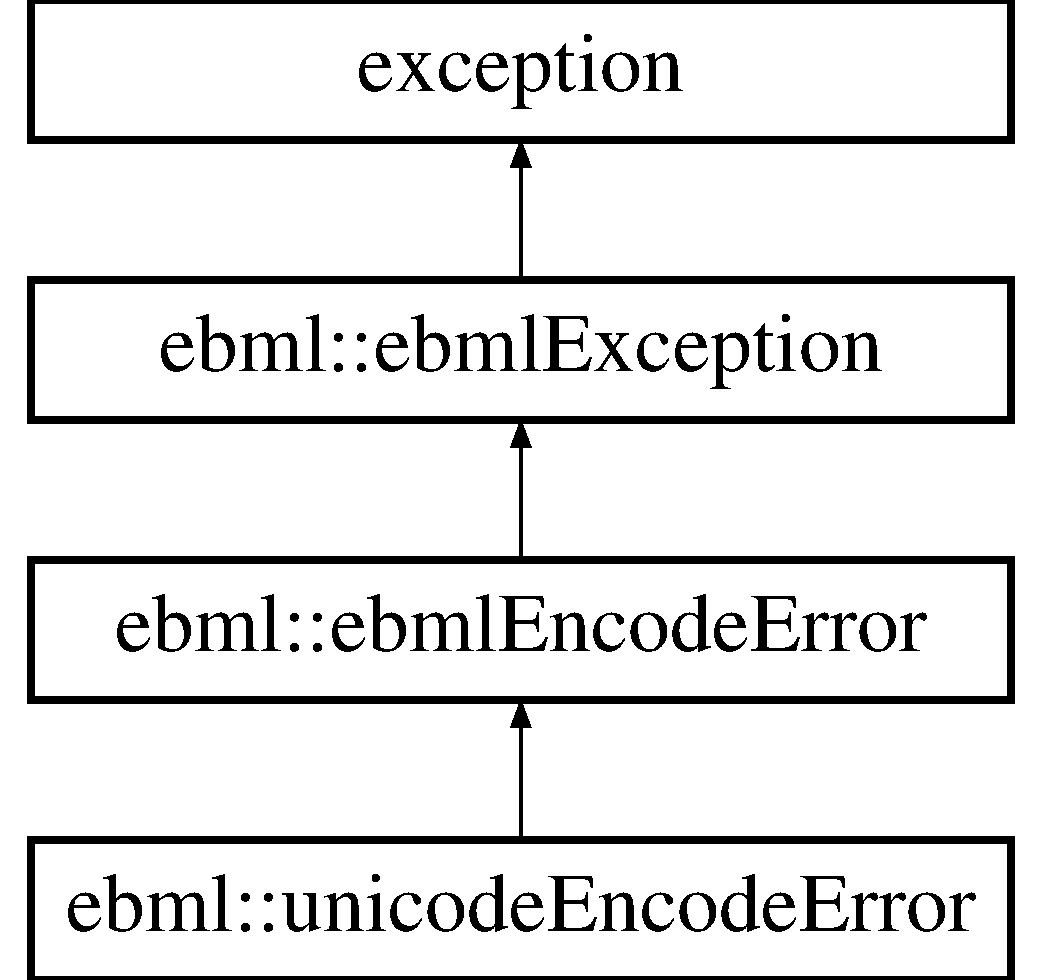
\includegraphics[height=4.000000cm]{classebml_1_1ebmlEncodeError}
\end{center}
\end{figure}
\subsection*{Public Member Functions}
\begin{DoxyCompactItemize}
\item 
\mbox{\hyperlink{classebml_1_1ebmlEncodeError_a18844f807f6e5a25283ed62ed59c4990}{ebml\+Encode\+Error}} (const std\+::string \&message, const \mbox{\hyperlink{namespaceebml_a2deef4e8071531b32e3533f1bf978917}{c\+\_\+ebml\+Element\+\_\+sp}} \&\mbox{\hyperlink{classebml_1_1ebmlEncodeError_acea050cc554e717e4d9845c0cf34d473}{elem}}=nullptr)
\item 
\mbox{\hyperlink{namespaceebml_a2deef4e8071531b32e3533f1bf978917}{c\+\_\+ebml\+Element\+\_\+sp}} \& \mbox{\hyperlink{classebml_1_1ebmlEncodeError_acea050cc554e717e4d9845c0cf34d473}{elem}} () const
\end{DoxyCompactItemize}


\subsection{Constructor \& Destructor Documentation}
\mbox{\Hypertarget{classebml_1_1ebmlEncodeError_a18844f807f6e5a25283ed62ed59c4990}\label{classebml_1_1ebmlEncodeError_a18844f807f6e5a25283ed62ed59c4990}} 
\index{ebml\+::ebml\+Encode\+Error@{ebml\+::ebml\+Encode\+Error}!ebml\+Encode\+Error@{ebml\+Encode\+Error}}
\index{ebml\+Encode\+Error@{ebml\+Encode\+Error}!ebml\+::ebml\+Encode\+Error@{ebml\+::ebml\+Encode\+Error}}
\subsubsection{\texorpdfstring{ebml\+Encode\+Error()}{ebmlEncodeError()}}
{\footnotesize\ttfamily ebml\+::ebml\+Encode\+Error\+::ebml\+Encode\+Error (\begin{DoxyParamCaption}\item[{const std\+::string \&}]{message,  }\item[{const \mbox{\hyperlink{namespaceebml_a2deef4e8071531b32e3533f1bf978917}{c\+\_\+ebml\+Element\+\_\+sp}} \&}]{elem = {\ttfamily nullptr} }\end{DoxyParamCaption})}



\subsection{Member Function Documentation}
\mbox{\Hypertarget{classebml_1_1ebmlEncodeError_acea050cc554e717e4d9845c0cf34d473}\label{classebml_1_1ebmlEncodeError_acea050cc554e717e4d9845c0cf34d473}} 
\index{ebml\+::ebml\+Encode\+Error@{ebml\+::ebml\+Encode\+Error}!elem@{elem}}
\index{elem@{elem}!ebml\+::ebml\+Encode\+Error@{ebml\+::ebml\+Encode\+Error}}
\subsubsection{\texorpdfstring{elem()}{elem()}}
{\footnotesize\ttfamily \mbox{\hyperlink{namespaceebml_a2deef4e8071531b32e3533f1bf978917}{c\+\_\+ebml\+Element\+\_\+sp}}\& ebml\+::ebml\+Encode\+Error\+::elem (\begin{DoxyParamCaption}{ }\end{DoxyParamCaption}) const}



The documentation for this class was generated from the following file\+:\begin{DoxyCompactItemize}
\item 
include/libebml\+\_\+ng/\mbox{\hyperlink{exceptions_8h}{exceptions.\+h}}\end{DoxyCompactItemize}

\hypertarget{classebml_1_1ebmlException}{}\section{ebml\+:\+:ebml\+Exception Class Reference}
\label{classebml_1_1ebmlException}\index{ebml\+::ebml\+Exception@{ebml\+::ebml\+Exception}}


{\ttfamily \#include $<$exceptions.\+h$>$}

Inheritance diagram for ebml\+:\+:ebml\+Exception\+:\begin{figure}[H]
\begin{center}
\leavevmode
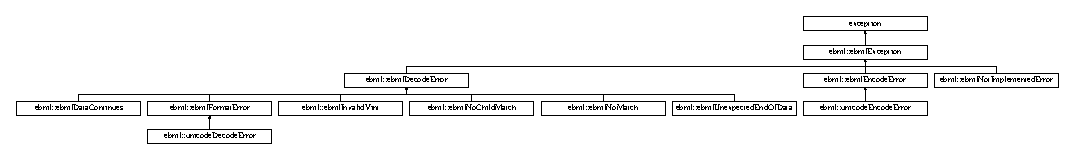
\includegraphics[height=1.699029cm]{classebml_1_1ebmlException}
\end{center}
\end{figure}
\subsection*{Public Member Functions}
\begin{DoxyCompactItemize}
\item 
\mbox{\hyperlink{classebml_1_1ebmlException_a0864653686e2432f259c8b3cbd5186af}{ebml\+Exception}} (const std\+::string \&message)
\item 
const char $\ast$ \mbox{\hyperlink{classebml_1_1ebmlException_a63892a18e5ba1fdee6abde1dd4869df8}{what}} () const noexcept override
\end{DoxyCompactItemize}


\subsection{Constructor \& Destructor Documentation}
\mbox{\Hypertarget{classebml_1_1ebmlException_a0864653686e2432f259c8b3cbd5186af}\label{classebml_1_1ebmlException_a0864653686e2432f259c8b3cbd5186af}} 
\index{ebml\+::ebml\+Exception@{ebml\+::ebml\+Exception}!ebml\+Exception@{ebml\+Exception}}
\index{ebml\+Exception@{ebml\+Exception}!ebml\+::ebml\+Exception@{ebml\+::ebml\+Exception}}
\subsubsection{\texorpdfstring{ebml\+Exception()}{ebmlException()}}
{\footnotesize\ttfamily ebml\+::ebml\+Exception\+::ebml\+Exception (\begin{DoxyParamCaption}\item[{const std\+::string \&}]{message }\end{DoxyParamCaption})}



\subsection{Member Function Documentation}
\mbox{\Hypertarget{classebml_1_1ebmlException_a63892a18e5ba1fdee6abde1dd4869df8}\label{classebml_1_1ebmlException_a63892a18e5ba1fdee6abde1dd4869df8}} 
\index{ebml\+::ebml\+Exception@{ebml\+::ebml\+Exception}!what@{what}}
\index{what@{what}!ebml\+::ebml\+Exception@{ebml\+::ebml\+Exception}}
\subsubsection{\texorpdfstring{what()}{what()}}
{\footnotesize\ttfamily const char$\ast$ ebml\+::ebml\+Exception\+::what (\begin{DoxyParamCaption}{ }\end{DoxyParamCaption}) const\hspace{0.3cm}{\ttfamily [override]}, {\ttfamily [noexcept]}}



The documentation for this class was generated from the following file\+:\begin{DoxyCompactItemize}
\item 
include/libebml\+\_\+ng/\mbox{\hyperlink{exceptions_8h}{exceptions.\+h}}\end{DoxyCompactItemize}

\hypertarget{classebml_1_1ebmlFormatError}{}\section{ebml\+:\+:ebml\+Format\+Error Class Reference}
\label{classebml_1_1ebmlFormatError}\index{ebml\+::ebml\+Format\+Error@{ebml\+::ebml\+Format\+Error}}


{\ttfamily \#include $<$exceptions.\+h$>$}

Inheritance diagram for ebml\+:\+:ebml\+Format\+Error\+:\begin{figure}[H]
\begin{center}
\leavevmode
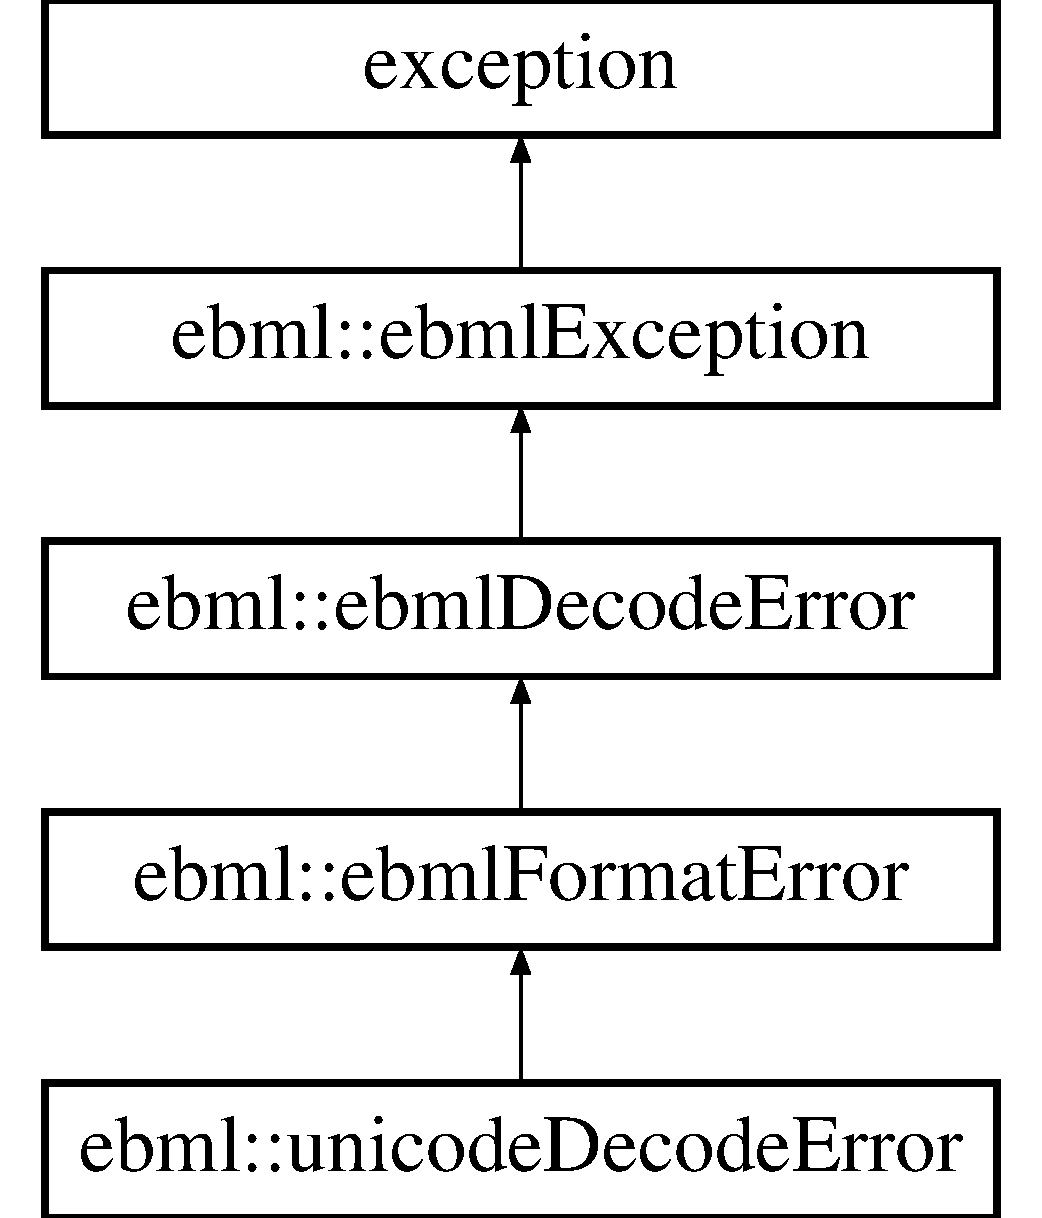
\includegraphics[height=5.000000cm]{classebml_1_1ebmlFormatError}
\end{center}
\end{figure}
\subsection*{Public Member Functions}
\begin{DoxyCompactItemize}
\item 
\mbox{\hyperlink{classebml_1_1ebmlFormatError_a49a8a445d4f385f34d79095504e2363d}{ebml\+Format\+Error}} (const std\+::string \&message, const \mbox{\hyperlink{classebml_1_1ebmlElementClass}{ebml\+Element\+Class}} $\ast$\mbox{\hyperlink{classebml_1_1ebmlDecodeError_a3568b4ea3cd5bd16b9510abfe269920f}{cls}}=nullptr, off\+\_\+t \mbox{\hyperlink{classebml_1_1ebmlDecodeError_ad32ac9b3dd52f1c11479085d9c665e0f}{offset}}=-\/1, unsigned char \mbox{\hyperlink{classebml_1_1ebmlDecodeError_a61a4d4856f0c779a1c216e45dc5a7c1e}{head\+Size}}=0, off\+\_\+t \mbox{\hyperlink{classebml_1_1ebmlDecodeError_acb525117e0109d9640fb5e8c546e9a02}{erroroffset}}=-\/1)
\end{DoxyCompactItemize}
\subsection*{Additional Inherited Members}


\subsection{Constructor \& Destructor Documentation}
\mbox{\Hypertarget{classebml_1_1ebmlFormatError_a49a8a445d4f385f34d79095504e2363d}\label{classebml_1_1ebmlFormatError_a49a8a445d4f385f34d79095504e2363d}} 
\index{ebml\+::ebml\+Format\+Error@{ebml\+::ebml\+Format\+Error}!ebml\+Format\+Error@{ebml\+Format\+Error}}
\index{ebml\+Format\+Error@{ebml\+Format\+Error}!ebml\+::ebml\+Format\+Error@{ebml\+::ebml\+Format\+Error}}
\subsubsection{\texorpdfstring{ebml\+Format\+Error()}{ebmlFormatError()}}
{\footnotesize\ttfamily ebml\+::ebml\+Format\+Error\+::ebml\+Format\+Error (\begin{DoxyParamCaption}\item[{const std\+::string \&}]{message,  }\item[{const \mbox{\hyperlink{classebml_1_1ebmlElementClass}{ebml\+Element\+Class}} $\ast$}]{cls = {\ttfamily nullptr},  }\item[{off\+\_\+t}]{offset = {\ttfamily -\/1},  }\item[{unsigned char}]{head\+Size = {\ttfamily 0},  }\item[{off\+\_\+t}]{erroroffset = {\ttfamily -\/1} }\end{DoxyParamCaption})}



The documentation for this class was generated from the following file\+:\begin{DoxyCompactItemize}
\item 
include/libebml\+\_\+ng/\mbox{\hyperlink{exceptions_8h}{exceptions.\+h}}\end{DoxyCompactItemize}

\hypertarget{classebml_1_1ebmlInvalidVint}{}\section{ebml\+:\+:ebml\+Invalid\+Vint Class Reference}
\label{classebml_1_1ebmlInvalidVint}\index{ebml\+::ebml\+Invalid\+Vint@{ebml\+::ebml\+Invalid\+Vint}}


{\ttfamily \#include $<$exceptions.\+h$>$}

Inheritance diagram for ebml\+:\+:ebml\+Invalid\+Vint\+:\begin{figure}[H]
\begin{center}
\leavevmode
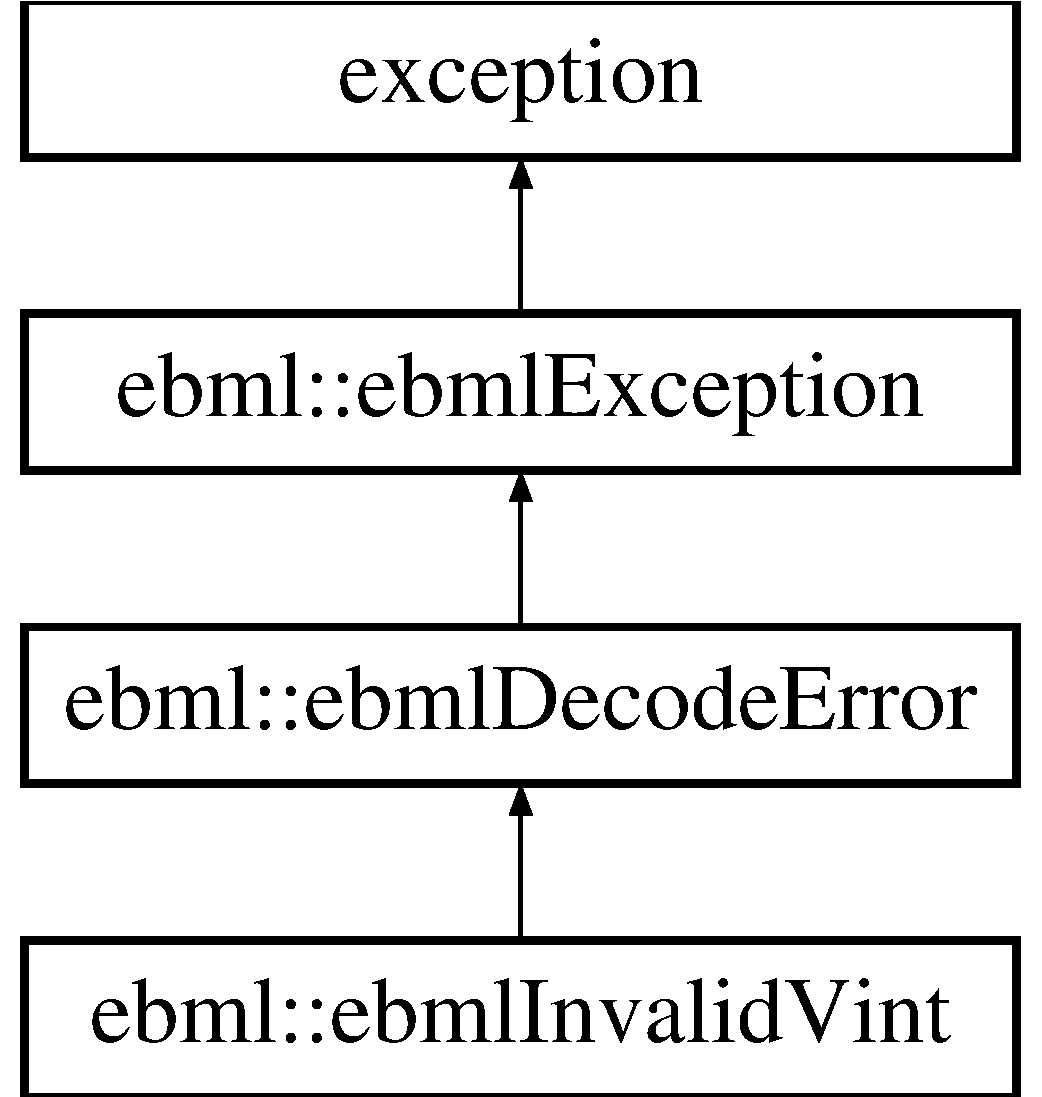
\includegraphics[height=4.000000cm]{classebml_1_1ebmlInvalidVint}
\end{center}
\end{figure}
\subsection*{Public Member Functions}
\begin{DoxyCompactItemize}
\item 
\mbox{\hyperlink{classebml_1_1ebmlInvalidVint_a8d8c4cbe43a5b4ab6d313a29f8249125}{ebml\+Invalid\+Vint}} (const std\+::string \&message, const \mbox{\hyperlink{classebml_1_1ebmlElementClass}{ebml\+Element\+Class}} $\ast$\mbox{\hyperlink{classebml_1_1ebmlDecodeError_a3568b4ea3cd5bd16b9510abfe269920f}{cls}}=nullptr, off\+\_\+t \mbox{\hyperlink{classebml_1_1ebmlDecodeError_ad32ac9b3dd52f1c11479085d9c665e0f}{offset}}=-\/1, unsigned char \mbox{\hyperlink{classebml_1_1ebmlDecodeError_a61a4d4856f0c779a1c216e45dc5a7c1e}{head\+Size}}=0, off\+\_\+t \mbox{\hyperlink{classebml_1_1ebmlDecodeError_acb525117e0109d9640fb5e8c546e9a02}{erroroffset}}=-\/1)
\end{DoxyCompactItemize}
\subsection*{Additional Inherited Members}


\subsection{Constructor \& Destructor Documentation}
\mbox{\Hypertarget{classebml_1_1ebmlInvalidVint_a8d8c4cbe43a5b4ab6d313a29f8249125}\label{classebml_1_1ebmlInvalidVint_a8d8c4cbe43a5b4ab6d313a29f8249125}} 
\index{ebml\+::ebml\+Invalid\+Vint@{ebml\+::ebml\+Invalid\+Vint}!ebml\+Invalid\+Vint@{ebml\+Invalid\+Vint}}
\index{ebml\+Invalid\+Vint@{ebml\+Invalid\+Vint}!ebml\+::ebml\+Invalid\+Vint@{ebml\+::ebml\+Invalid\+Vint}}
\subsubsection{\texorpdfstring{ebml\+Invalid\+Vint()}{ebmlInvalidVint()}}
{\footnotesize\ttfamily ebml\+::ebml\+Invalid\+Vint\+::ebml\+Invalid\+Vint (\begin{DoxyParamCaption}\item[{const std\+::string \&}]{message,  }\item[{const \mbox{\hyperlink{classebml_1_1ebmlElementClass}{ebml\+Element\+Class}} $\ast$}]{cls = {\ttfamily nullptr},  }\item[{off\+\_\+t}]{offset = {\ttfamily -\/1},  }\item[{unsigned char}]{head\+Size = {\ttfamily 0},  }\item[{off\+\_\+t}]{erroroffset = {\ttfamily -\/1} }\end{DoxyParamCaption})}



The documentation for this class was generated from the following file\+:\begin{DoxyCompactItemize}
\item 
include/libebml\+\_\+ng/\mbox{\hyperlink{exceptions_8h}{exceptions.\+h}}\end{DoxyCompactItemize}

\input{classebml_1_1ebmlLazyLoad}
\input{classebml_1_1ebmlLazyLoadClass}
\hypertarget{classebml_1_1ebmlList}{}\section{ebml\+:\+:ebml\+List Class Reference}
\label{classebml_1_1ebmlList}\index{ebml\+::ebml\+List@{ebml\+::ebml\+List}}


{\ttfamily \#include $<$list.\+h$>$}

Inheritance diagram for ebml\+:\+:ebml\+List\+:\begin{figure}[H]
\begin{center}
\leavevmode
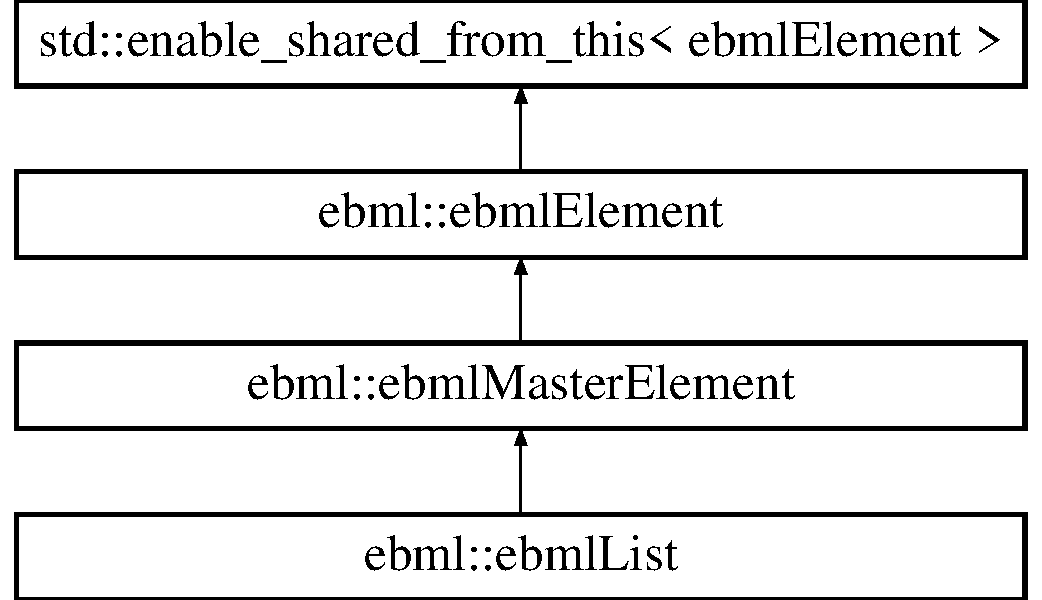
\includegraphics[height=4.000000cm]{classebml_1_1ebmlList}
\end{center}
\end{figure}
\subsection*{Classes}
\begin{DoxyCompactItemize}
\item 
class \mbox{\hyperlink{classebml_1_1ebmlList_1_1__const__iterator}{\+\_\+const\+\_\+iterator}}
\item 
class \mbox{\hyperlink{classebml_1_1ebmlList_1_1__iterator}{\+\_\+iterator}}
\end{DoxyCompactItemize}
\subsection*{Public Member Functions}
\begin{DoxyCompactItemize}
\item 
void \mbox{\hyperlink{classebml_1_1ebmlList_aa94bbf1188e309c806198c179dc57149}{set\+Data}} (const \mbox{\hyperlink{namespaceebml_a1ddadd26791f273d851882653b9caf70}{ebml\+Element\+\_\+l}} \&)
\item 
void \mbox{\hyperlink{classebml_1_1ebmlList_a4fe5b352155dd7180522e85ec7d7f865}{set\+Data}} (\mbox{\hyperlink{namespaceebml_a1ddadd26791f273d851882653b9caf70}{ebml\+Element\+\_\+l}} \&\&)
\item 
std\+::wstring \mbox{\hyperlink{classebml_1_1ebmlList_a49cf343c62058b121e7c546e8afa0947}{minirepr}} () const override
\item 
\mbox{\hyperlink{classebml_1_1childSlot__t}{child\+Slot\+\_\+t}} \mbox{\hyperlink{classebml_1_1ebmlList_a93db5aabab62f6761162e2add92cdda7}{operator\mbox{[}$\,$\mbox{]}}} (off\+\_\+t)
\item 
\mbox{\hyperlink{classebml_1_1childSlot__t}{child\+Slot\+\_\+t}} \mbox{\hyperlink{classebml_1_1ebmlList_af07f5e6d2e1e9d7f2f85c49447aefec1}{at}} (off\+\_\+t)
\item 
\mbox{\hyperlink{classebml_1_1childSlot__t}{child\+Slot\+\_\+t}} \mbox{\hyperlink{classebml_1_1ebmlList_a099cd0a5c21fb83a005638fa8990ae8c}{front}} ()
\item 
\mbox{\hyperlink{classebml_1_1childSlot__t}{child\+Slot\+\_\+t}} \mbox{\hyperlink{classebml_1_1ebmlList_a038cf53176c9e4cf80930e7deef86714}{back}} ()
\item 
\mbox{\hyperlink{namespaceebml_a2deef4e8071531b32e3533f1bf978917}{c\+\_\+ebml\+Element\+\_\+sp}} \mbox{\hyperlink{classebml_1_1ebmlList_ad1960e8d6774b85ab02b86981a661196}{operator\mbox{[}$\,$\mbox{]}}} (off\+\_\+t) const
\item 
\mbox{\hyperlink{namespaceebml_a2deef4e8071531b32e3533f1bf978917}{c\+\_\+ebml\+Element\+\_\+sp}} \mbox{\hyperlink{classebml_1_1ebmlList_aee4aa9a8875e80e6a6583d85e86fe7f5}{at}} (off\+\_\+t) const
\item 
\mbox{\hyperlink{namespaceebml_a2deef4e8071531b32e3533f1bf978917}{c\+\_\+ebml\+Element\+\_\+sp}} \mbox{\hyperlink{classebml_1_1ebmlList_add75b2ad61fe9f997df303872adc67da}{front}} () const
\item 
\mbox{\hyperlink{namespaceebml_a2deef4e8071531b32e3533f1bf978917}{c\+\_\+ebml\+Element\+\_\+sp}} \mbox{\hyperlink{classebml_1_1ebmlList_a3ae9e052dca738b1a3e66c9da0e47e76}{back}} () const
\item 
bool \mbox{\hyperlink{classebml_1_1ebmlList_abab676e25a152cba3818e54d32cbfe35}{contains}} (const \mbox{\hyperlink{namespaceebml_a2deef4e8071531b32e3533f1bf978917}{c\+\_\+ebml\+Element\+\_\+sp}} \&) const
\item 
off\+\_\+t \mbox{\hyperlink{classebml_1_1ebmlList_a2f680a149168b81adfb6e85b7af8e272}{index}} (const \mbox{\hyperlink{namespaceebml_a2deef4e8071531b32e3533f1bf978917}{c\+\_\+ebml\+Element\+\_\+sp}} \&) const
\item 
void \mbox{\hyperlink{classebml_1_1ebmlList_ab13093132d1a49a67837fd51e6abc8af}{push\+\_\+back}} (const \mbox{\hyperlink{namespaceebml_adad533b7705a16bb360fe56380c5e7be}{ebml\+Element\+\_\+sp}} \&)
\item 
void \mbox{\hyperlink{classebml_1_1ebmlList_aa96dd50adeed937177a8addc38daf3f0}{push\+\_\+back}} (\mbox{\hyperlink{namespaceebml_adad533b7705a16bb360fe56380c5e7be}{ebml\+Element\+\_\+sp}} \&\&)
\item 
void \mbox{\hyperlink{classebml_1_1ebmlList_a02685f24e74011cb4798467e7041c472}{pop\+\_\+back}} ()
\item 
void \mbox{\hyperlink{classebml_1_1ebmlList_abc0424061c7edb3ecdfd5169f7de7288}{insert}} (off\+\_\+t, const \mbox{\hyperlink{namespaceebml_adad533b7705a16bb360fe56380c5e7be}{ebml\+Element\+\_\+sp}} \&)
\item 
void \mbox{\hyperlink{classebml_1_1ebmlList_a7dc291c779b8e3e389a68caf8266ebf3}{insert}} (off\+\_\+t, \mbox{\hyperlink{namespaceebml_adad533b7705a16bb360fe56380c5e7be}{ebml\+Element\+\_\+sp}} \&\&)
\item 
void \mbox{\hyperlink{classebml_1_1ebmlList_a5b2db67357ddbee4801414fed4fb1640}{erase}} (off\+\_\+t)
\item 
void \mbox{\hyperlink{classebml_1_1ebmlList_a757aaf37e69f54397c74fab476c0cdc1}{clear}} ()
\item 
size\+\_\+t \mbox{\hyperlink{classebml_1_1ebmlList_a9537fed381f80c9d06fdd2ccb08a42b2}{size}} () const
\end{DoxyCompactItemize}
\subsection*{Protected Member Functions}
\begin{DoxyCompactItemize}
\item 
\mbox{\hyperlink{classebml_1_1ebmlList_a8df16a98de7ff5cd9512840b908b1247}{ebml\+List}} (const \mbox{\hyperlink{classebml_1_1ebmlListClass}{ebml\+List\+Class}} $\ast$)
\item 
void \mbox{\hyperlink{classebml_1_1ebmlList_a2e57019d123e9647b47148c6f827cbed}{\+\_\+clear}} () override
\item 
void \mbox{\hyperlink{classebml_1_1ebmlList_a438c83de7e7fe38aced71d9ad27d29b9}{\+\_\+validate\+Data}} (const \mbox{\hyperlink{namespaceebml_a1ddadd26791f273d851882653b9caf70}{ebml\+Element\+\_\+l}} \&)
\item 
void \mbox{\hyperlink{classebml_1_1ebmlList_a366d78242b59ec90774774cd278e5863}{\+\_\+set\+Data}} (const \mbox{\hyperlink{namespaceebml_a1ddadd26791f273d851882653b9caf70}{ebml\+Element\+\_\+l}} \&)
\item 
void \mbox{\hyperlink{classebml_1_1ebmlList_af612aabfde64c4ef1c93ad7c16e76aa5}{\+\_\+set\+Data}} (\mbox{\hyperlink{namespaceebml_a1ddadd26791f273d851882653b9caf70}{ebml\+Element\+\_\+l}} \&\&)
\item 
\mbox{\hyperlink{classebml_1_1ebmlMasterElement_1_1__iterator}{ebml\+Master\+Element\+::\+\_\+iterator}} $\ast$ \mbox{\hyperlink{classebml_1_1ebmlList_a95b8de53fe3688ba73ee488e8ca94566}{\+\_\+begin}} () override
\item 
\mbox{\hyperlink{classebml_1_1ebmlMasterElement_1_1__iterator}{ebml\+Master\+Element\+::\+\_\+iterator}} $\ast$ \mbox{\hyperlink{classebml_1_1ebmlList_aec7a5554e1d10fd7575104471cb2c6f4}{\+\_\+end}} () override
\item 
\mbox{\hyperlink{classebml_1_1ebmlMasterElement_1_1__const__iterator}{ebml\+Master\+Element\+::\+\_\+const\+\_\+iterator}} $\ast$ \mbox{\hyperlink{classebml_1_1ebmlList_a7f215c99205ac37681fe7314463171bc}{\+\_\+cbegin}} () const override
\item 
\mbox{\hyperlink{classebml_1_1ebmlMasterElement_1_1__const__iterator}{ebml\+Master\+Element\+::\+\_\+const\+\_\+iterator}} $\ast$ \mbox{\hyperlink{classebml_1_1ebmlList_abfda97c7cfa6ab0328b444b7ae832b64}{\+\_\+cend}} () const override
\item 
void \mbox{\hyperlink{classebml_1_1ebmlList_aafcb7a3112a89b0bdde898b84ee44ec5}{\+\_\+add\+Child}} (const \mbox{\hyperlink{namespaceebml_adad533b7705a16bb360fe56380c5e7be}{ebml\+Element\+\_\+sp}} \&) override
\item 
void \mbox{\hyperlink{classebml_1_1ebmlList_a372e75614d5c93b7d7a55548c45c2d2f}{\+\_\+add\+Child}} (\mbox{\hyperlink{namespaceebml_adad533b7705a16bb360fe56380c5e7be}{ebml\+Element\+\_\+sp}} \&\&) override
\end{DoxyCompactItemize}
\subsection*{Friends}
\begin{DoxyCompactItemize}
\item 
class \mbox{\hyperlink{classebml_1_1ebmlList_a97c631dff45f04b8ed9b303d6a9e03c5}{ebml\+List\+Class}}
\item 
{\footnotesize template$<$typename T , typename U , typename... Args$>$ }\\std\+::shared\+\_\+ptr$<$ U $>$ \mbox{\hyperlink{classebml_1_1ebmlList_ace404b6adc012cac5ccd9c03160456e3}{new\+\_\+sp}} (Args... args)
\end{DoxyCompactItemize}
\subsection*{Additional Inherited Members}


\subsection{Constructor \& Destructor Documentation}
\mbox{\Hypertarget{classebml_1_1ebmlList_a8df16a98de7ff5cd9512840b908b1247}\label{classebml_1_1ebmlList_a8df16a98de7ff5cd9512840b908b1247}} 
\index{ebml\+::ebml\+List@{ebml\+::ebml\+List}!ebml\+List@{ebml\+List}}
\index{ebml\+List@{ebml\+List}!ebml\+::ebml\+List@{ebml\+::ebml\+List}}
\subsubsection{\texorpdfstring{ebml\+List()}{ebmlList()}}
{\footnotesize\ttfamily ebml\+::ebml\+List\+::ebml\+List (\begin{DoxyParamCaption}\item[{const \mbox{\hyperlink{classebml_1_1ebmlListClass}{ebml\+List\+Class}} $\ast$}]{ }\end{DoxyParamCaption})\hspace{0.3cm}{\ttfamily [protected]}}



\subsection{Member Function Documentation}
\mbox{\Hypertarget{classebml_1_1ebmlList_aafcb7a3112a89b0bdde898b84ee44ec5}\label{classebml_1_1ebmlList_aafcb7a3112a89b0bdde898b84ee44ec5}} 
\index{ebml\+::ebml\+List@{ebml\+::ebml\+List}!\+\_\+add\+Child@{\+\_\+add\+Child}}
\index{\+\_\+add\+Child@{\+\_\+add\+Child}!ebml\+::ebml\+List@{ebml\+::ebml\+List}}
\subsubsection{\texorpdfstring{\+\_\+add\+Child()}{\_addChild()}\hspace{0.1cm}{\footnotesize\ttfamily [1/2]}}
{\footnotesize\ttfamily void ebml\+::ebml\+List\+::\+\_\+add\+Child (\begin{DoxyParamCaption}\item[{const \mbox{\hyperlink{namespaceebml_adad533b7705a16bb360fe56380c5e7be}{ebml\+Element\+\_\+sp}} \&}]{ }\end{DoxyParamCaption})\hspace{0.3cm}{\ttfamily [override]}, {\ttfamily [protected]}, {\ttfamily [virtual]}}



Implements \mbox{\hyperlink{classebml_1_1ebmlMasterElement_a59c5f3b3409fd5fd6f0f22c7a68f1c9b}{ebml\+::ebml\+Master\+Element}}.

\mbox{\Hypertarget{classebml_1_1ebmlList_a372e75614d5c93b7d7a55548c45c2d2f}\label{classebml_1_1ebmlList_a372e75614d5c93b7d7a55548c45c2d2f}} 
\index{ebml\+::ebml\+List@{ebml\+::ebml\+List}!\+\_\+add\+Child@{\+\_\+add\+Child}}
\index{\+\_\+add\+Child@{\+\_\+add\+Child}!ebml\+::ebml\+List@{ebml\+::ebml\+List}}
\subsubsection{\texorpdfstring{\+\_\+add\+Child()}{\_addChild()}\hspace{0.1cm}{\footnotesize\ttfamily [2/2]}}
{\footnotesize\ttfamily void ebml\+::ebml\+List\+::\+\_\+add\+Child (\begin{DoxyParamCaption}\item[{\mbox{\hyperlink{namespaceebml_adad533b7705a16bb360fe56380c5e7be}{ebml\+Element\+\_\+sp}} \&\&}]{ }\end{DoxyParamCaption})\hspace{0.3cm}{\ttfamily [override]}, {\ttfamily [protected]}, {\ttfamily [virtual]}}



Implements \mbox{\hyperlink{classebml_1_1ebmlMasterElement_a3af0270846a1ced1719d26dd261f0355}{ebml\+::ebml\+Master\+Element}}.

\mbox{\Hypertarget{classebml_1_1ebmlList_a95b8de53fe3688ba73ee488e8ca94566}\label{classebml_1_1ebmlList_a95b8de53fe3688ba73ee488e8ca94566}} 
\index{ebml\+::ebml\+List@{ebml\+::ebml\+List}!\+\_\+begin@{\+\_\+begin}}
\index{\+\_\+begin@{\+\_\+begin}!ebml\+::ebml\+List@{ebml\+::ebml\+List}}
\subsubsection{\texorpdfstring{\+\_\+begin()}{\_begin()}}
{\footnotesize\ttfamily \mbox{\hyperlink{classebml_1_1ebmlMasterElement_1_1__iterator}{ebml\+Master\+Element\+::\+\_\+iterator}}$\ast$ ebml\+::ebml\+List\+::\+\_\+begin (\begin{DoxyParamCaption}{ }\end{DoxyParamCaption})\hspace{0.3cm}{\ttfamily [override]}, {\ttfamily [protected]}, {\ttfamily [virtual]}}



Implements \mbox{\hyperlink{classebml_1_1ebmlMasterElement_af6fb7a9934e9b8d0c64273ef6944f44b}{ebml\+::ebml\+Master\+Element}}.

\mbox{\Hypertarget{classebml_1_1ebmlList_a7f215c99205ac37681fe7314463171bc}\label{classebml_1_1ebmlList_a7f215c99205ac37681fe7314463171bc}} 
\index{ebml\+::ebml\+List@{ebml\+::ebml\+List}!\+\_\+cbegin@{\+\_\+cbegin}}
\index{\+\_\+cbegin@{\+\_\+cbegin}!ebml\+::ebml\+List@{ebml\+::ebml\+List}}
\subsubsection{\texorpdfstring{\+\_\+cbegin()}{\_cbegin()}}
{\footnotesize\ttfamily \mbox{\hyperlink{classebml_1_1ebmlMasterElement_1_1__const__iterator}{ebml\+Master\+Element\+::\+\_\+const\+\_\+iterator}}$\ast$ ebml\+::ebml\+List\+::\+\_\+cbegin (\begin{DoxyParamCaption}{ }\end{DoxyParamCaption}) const\hspace{0.3cm}{\ttfamily [override]}, {\ttfamily [protected]}, {\ttfamily [virtual]}}



Implements \mbox{\hyperlink{classebml_1_1ebmlMasterElement_a7e1ffa498e22b637a6671df14aa0bc45}{ebml\+::ebml\+Master\+Element}}.

\mbox{\Hypertarget{classebml_1_1ebmlList_abfda97c7cfa6ab0328b444b7ae832b64}\label{classebml_1_1ebmlList_abfda97c7cfa6ab0328b444b7ae832b64}} 
\index{ebml\+::ebml\+List@{ebml\+::ebml\+List}!\+\_\+cend@{\+\_\+cend}}
\index{\+\_\+cend@{\+\_\+cend}!ebml\+::ebml\+List@{ebml\+::ebml\+List}}
\subsubsection{\texorpdfstring{\+\_\+cend()}{\_cend()}}
{\footnotesize\ttfamily \mbox{\hyperlink{classebml_1_1ebmlMasterElement_1_1__const__iterator}{ebml\+Master\+Element\+::\+\_\+const\+\_\+iterator}}$\ast$ ebml\+::ebml\+List\+::\+\_\+cend (\begin{DoxyParamCaption}{ }\end{DoxyParamCaption}) const\hspace{0.3cm}{\ttfamily [override]}, {\ttfamily [protected]}, {\ttfamily [virtual]}}



Implements \mbox{\hyperlink{classebml_1_1ebmlMasterElement_ae6cdbf68d8267a7ab098bd402fa70e88}{ebml\+::ebml\+Master\+Element}}.

\mbox{\Hypertarget{classebml_1_1ebmlList_a2e57019d123e9647b47148c6f827cbed}\label{classebml_1_1ebmlList_a2e57019d123e9647b47148c6f827cbed}} 
\index{ebml\+::ebml\+List@{ebml\+::ebml\+List}!\+\_\+clear@{\+\_\+clear}}
\index{\+\_\+clear@{\+\_\+clear}!ebml\+::ebml\+List@{ebml\+::ebml\+List}}
\subsubsection{\texorpdfstring{\+\_\+clear()}{\_clear()}}
{\footnotesize\ttfamily void ebml\+::ebml\+List\+::\+\_\+clear (\begin{DoxyParamCaption}{ }\end{DoxyParamCaption})\hspace{0.3cm}{\ttfamily [override]}, {\ttfamily [protected]}, {\ttfamily [virtual]}}



Reimplemented from \mbox{\hyperlink{classebml_1_1ebmlMasterElement_a2fdf9fa1022f06a046fe94e631e266a3}{ebml\+::ebml\+Master\+Element}}.

\mbox{\Hypertarget{classebml_1_1ebmlList_aec7a5554e1d10fd7575104471cb2c6f4}\label{classebml_1_1ebmlList_aec7a5554e1d10fd7575104471cb2c6f4}} 
\index{ebml\+::ebml\+List@{ebml\+::ebml\+List}!\+\_\+end@{\+\_\+end}}
\index{\+\_\+end@{\+\_\+end}!ebml\+::ebml\+List@{ebml\+::ebml\+List}}
\subsubsection{\texorpdfstring{\+\_\+end()}{\_end()}}
{\footnotesize\ttfamily \mbox{\hyperlink{classebml_1_1ebmlMasterElement_1_1__iterator}{ebml\+Master\+Element\+::\+\_\+iterator}}$\ast$ ebml\+::ebml\+List\+::\+\_\+end (\begin{DoxyParamCaption}{ }\end{DoxyParamCaption})\hspace{0.3cm}{\ttfamily [override]}, {\ttfamily [protected]}, {\ttfamily [virtual]}}



Implements \mbox{\hyperlink{classebml_1_1ebmlMasterElement_a352e5e11836063394990cb05c09d8e48}{ebml\+::ebml\+Master\+Element}}.

\mbox{\Hypertarget{classebml_1_1ebmlList_a366d78242b59ec90774774cd278e5863}\label{classebml_1_1ebmlList_a366d78242b59ec90774774cd278e5863}} 
\index{ebml\+::ebml\+List@{ebml\+::ebml\+List}!\+\_\+set\+Data@{\+\_\+set\+Data}}
\index{\+\_\+set\+Data@{\+\_\+set\+Data}!ebml\+::ebml\+List@{ebml\+::ebml\+List}}
\subsubsection{\texorpdfstring{\+\_\+set\+Data()}{\_setData()}\hspace{0.1cm}{\footnotesize\ttfamily [1/2]}}
{\footnotesize\ttfamily void ebml\+::ebml\+List\+::\+\_\+set\+Data (\begin{DoxyParamCaption}\item[{const \mbox{\hyperlink{namespaceebml_a1ddadd26791f273d851882653b9caf70}{ebml\+Element\+\_\+l}} \&}]{ }\end{DoxyParamCaption})\hspace{0.3cm}{\ttfamily [protected]}}

\mbox{\Hypertarget{classebml_1_1ebmlList_af612aabfde64c4ef1c93ad7c16e76aa5}\label{classebml_1_1ebmlList_af612aabfde64c4ef1c93ad7c16e76aa5}} 
\index{ebml\+::ebml\+List@{ebml\+::ebml\+List}!\+\_\+set\+Data@{\+\_\+set\+Data}}
\index{\+\_\+set\+Data@{\+\_\+set\+Data}!ebml\+::ebml\+List@{ebml\+::ebml\+List}}
\subsubsection{\texorpdfstring{\+\_\+set\+Data()}{\_setData()}\hspace{0.1cm}{\footnotesize\ttfamily [2/2]}}
{\footnotesize\ttfamily void ebml\+::ebml\+List\+::\+\_\+set\+Data (\begin{DoxyParamCaption}\item[{\mbox{\hyperlink{namespaceebml_a1ddadd26791f273d851882653b9caf70}{ebml\+Element\+\_\+l}} \&\&}]{ }\end{DoxyParamCaption})\hspace{0.3cm}{\ttfamily [protected]}}

\mbox{\Hypertarget{classebml_1_1ebmlList_a438c83de7e7fe38aced71d9ad27d29b9}\label{classebml_1_1ebmlList_a438c83de7e7fe38aced71d9ad27d29b9}} 
\index{ebml\+::ebml\+List@{ebml\+::ebml\+List}!\+\_\+validate\+Data@{\+\_\+validate\+Data}}
\index{\+\_\+validate\+Data@{\+\_\+validate\+Data}!ebml\+::ebml\+List@{ebml\+::ebml\+List}}
\subsubsection{\texorpdfstring{\+\_\+validate\+Data()}{\_validateData()}}
{\footnotesize\ttfamily void ebml\+::ebml\+List\+::\+\_\+validate\+Data (\begin{DoxyParamCaption}\item[{const \mbox{\hyperlink{namespaceebml_a1ddadd26791f273d851882653b9caf70}{ebml\+Element\+\_\+l}} \&}]{ }\end{DoxyParamCaption})\hspace{0.3cm}{\ttfamily [protected]}}

\mbox{\Hypertarget{classebml_1_1ebmlList_af07f5e6d2e1e9d7f2f85c49447aefec1}\label{classebml_1_1ebmlList_af07f5e6d2e1e9d7f2f85c49447aefec1}} 
\index{ebml\+::ebml\+List@{ebml\+::ebml\+List}!at@{at}}
\index{at@{at}!ebml\+::ebml\+List@{ebml\+::ebml\+List}}
\subsubsection{\texorpdfstring{at()}{at()}\hspace{0.1cm}{\footnotesize\ttfamily [1/2]}}
{\footnotesize\ttfamily \mbox{\hyperlink{classebml_1_1childSlot__t}{child\+Slot\+\_\+t}} ebml\+::ebml\+List\+::at (\begin{DoxyParamCaption}\item[{off\+\_\+t}]{ }\end{DoxyParamCaption})}

\mbox{\Hypertarget{classebml_1_1ebmlList_aee4aa9a8875e80e6a6583d85e86fe7f5}\label{classebml_1_1ebmlList_aee4aa9a8875e80e6a6583d85e86fe7f5}} 
\index{ebml\+::ebml\+List@{ebml\+::ebml\+List}!at@{at}}
\index{at@{at}!ebml\+::ebml\+List@{ebml\+::ebml\+List}}
\subsubsection{\texorpdfstring{at()}{at()}\hspace{0.1cm}{\footnotesize\ttfamily [2/2]}}
{\footnotesize\ttfamily \mbox{\hyperlink{namespaceebml_a2deef4e8071531b32e3533f1bf978917}{c\+\_\+ebml\+Element\+\_\+sp}} ebml\+::ebml\+List\+::at (\begin{DoxyParamCaption}\item[{off\+\_\+t}]{ }\end{DoxyParamCaption}) const}

\mbox{\Hypertarget{classebml_1_1ebmlList_a038cf53176c9e4cf80930e7deef86714}\label{classebml_1_1ebmlList_a038cf53176c9e4cf80930e7deef86714}} 
\index{ebml\+::ebml\+List@{ebml\+::ebml\+List}!back@{back}}
\index{back@{back}!ebml\+::ebml\+List@{ebml\+::ebml\+List}}
\subsubsection{\texorpdfstring{back()}{back()}\hspace{0.1cm}{\footnotesize\ttfamily [1/2]}}
{\footnotesize\ttfamily \mbox{\hyperlink{classebml_1_1childSlot__t}{child\+Slot\+\_\+t}} ebml\+::ebml\+List\+::back (\begin{DoxyParamCaption}{ }\end{DoxyParamCaption})}

\mbox{\Hypertarget{classebml_1_1ebmlList_a3ae9e052dca738b1a3e66c9da0e47e76}\label{classebml_1_1ebmlList_a3ae9e052dca738b1a3e66c9da0e47e76}} 
\index{ebml\+::ebml\+List@{ebml\+::ebml\+List}!back@{back}}
\index{back@{back}!ebml\+::ebml\+List@{ebml\+::ebml\+List}}
\subsubsection{\texorpdfstring{back()}{back()}\hspace{0.1cm}{\footnotesize\ttfamily [2/2]}}
{\footnotesize\ttfamily \mbox{\hyperlink{namespaceebml_a2deef4e8071531b32e3533f1bf978917}{c\+\_\+ebml\+Element\+\_\+sp}} ebml\+::ebml\+List\+::back (\begin{DoxyParamCaption}{ }\end{DoxyParamCaption}) const}

\mbox{\Hypertarget{classebml_1_1ebmlList_a757aaf37e69f54397c74fab476c0cdc1}\label{classebml_1_1ebmlList_a757aaf37e69f54397c74fab476c0cdc1}} 
\index{ebml\+::ebml\+List@{ebml\+::ebml\+List}!clear@{clear}}
\index{clear@{clear}!ebml\+::ebml\+List@{ebml\+::ebml\+List}}
\subsubsection{\texorpdfstring{clear()}{clear()}}
{\footnotesize\ttfamily void ebml\+::ebml\+List\+::clear (\begin{DoxyParamCaption}{ }\end{DoxyParamCaption})}

\mbox{\Hypertarget{classebml_1_1ebmlList_abab676e25a152cba3818e54d32cbfe35}\label{classebml_1_1ebmlList_abab676e25a152cba3818e54d32cbfe35}} 
\index{ebml\+::ebml\+List@{ebml\+::ebml\+List}!contains@{contains}}
\index{contains@{contains}!ebml\+::ebml\+List@{ebml\+::ebml\+List}}
\subsubsection{\texorpdfstring{contains()}{contains()}}
{\footnotesize\ttfamily bool ebml\+::ebml\+List\+::contains (\begin{DoxyParamCaption}\item[{const \mbox{\hyperlink{namespaceebml_a2deef4e8071531b32e3533f1bf978917}{c\+\_\+ebml\+Element\+\_\+sp}} \&}]{ }\end{DoxyParamCaption}) const}

\mbox{\Hypertarget{classebml_1_1ebmlList_a5b2db67357ddbee4801414fed4fb1640}\label{classebml_1_1ebmlList_a5b2db67357ddbee4801414fed4fb1640}} 
\index{ebml\+::ebml\+List@{ebml\+::ebml\+List}!erase@{erase}}
\index{erase@{erase}!ebml\+::ebml\+List@{ebml\+::ebml\+List}}
\subsubsection{\texorpdfstring{erase()}{erase()}}
{\footnotesize\ttfamily void ebml\+::ebml\+List\+::erase (\begin{DoxyParamCaption}\item[{off\+\_\+t}]{ }\end{DoxyParamCaption})}

\mbox{\Hypertarget{classebml_1_1ebmlList_a099cd0a5c21fb83a005638fa8990ae8c}\label{classebml_1_1ebmlList_a099cd0a5c21fb83a005638fa8990ae8c}} 
\index{ebml\+::ebml\+List@{ebml\+::ebml\+List}!front@{front}}
\index{front@{front}!ebml\+::ebml\+List@{ebml\+::ebml\+List}}
\subsubsection{\texorpdfstring{front()}{front()}\hspace{0.1cm}{\footnotesize\ttfamily [1/2]}}
{\footnotesize\ttfamily \mbox{\hyperlink{classebml_1_1childSlot__t}{child\+Slot\+\_\+t}} ebml\+::ebml\+List\+::front (\begin{DoxyParamCaption}{ }\end{DoxyParamCaption})}

\mbox{\Hypertarget{classebml_1_1ebmlList_add75b2ad61fe9f997df303872adc67da}\label{classebml_1_1ebmlList_add75b2ad61fe9f997df303872adc67da}} 
\index{ebml\+::ebml\+List@{ebml\+::ebml\+List}!front@{front}}
\index{front@{front}!ebml\+::ebml\+List@{ebml\+::ebml\+List}}
\subsubsection{\texorpdfstring{front()}{front()}\hspace{0.1cm}{\footnotesize\ttfamily [2/2]}}
{\footnotesize\ttfamily \mbox{\hyperlink{namespaceebml_a2deef4e8071531b32e3533f1bf978917}{c\+\_\+ebml\+Element\+\_\+sp}} ebml\+::ebml\+List\+::front (\begin{DoxyParamCaption}{ }\end{DoxyParamCaption}) const}

\mbox{\Hypertarget{classebml_1_1ebmlList_a2f680a149168b81adfb6e85b7af8e272}\label{classebml_1_1ebmlList_a2f680a149168b81adfb6e85b7af8e272}} 
\index{ebml\+::ebml\+List@{ebml\+::ebml\+List}!index@{index}}
\index{index@{index}!ebml\+::ebml\+List@{ebml\+::ebml\+List}}
\subsubsection{\texorpdfstring{index()}{index()}}
{\footnotesize\ttfamily off\+\_\+t ebml\+::ebml\+List\+::index (\begin{DoxyParamCaption}\item[{const \mbox{\hyperlink{namespaceebml_a2deef4e8071531b32e3533f1bf978917}{c\+\_\+ebml\+Element\+\_\+sp}} \&}]{ }\end{DoxyParamCaption}) const}

\mbox{\Hypertarget{classebml_1_1ebmlList_abc0424061c7edb3ecdfd5169f7de7288}\label{classebml_1_1ebmlList_abc0424061c7edb3ecdfd5169f7de7288}} 
\index{ebml\+::ebml\+List@{ebml\+::ebml\+List}!insert@{insert}}
\index{insert@{insert}!ebml\+::ebml\+List@{ebml\+::ebml\+List}}
\subsubsection{\texorpdfstring{insert()}{insert()}\hspace{0.1cm}{\footnotesize\ttfamily [1/2]}}
{\footnotesize\ttfamily void ebml\+::ebml\+List\+::insert (\begin{DoxyParamCaption}\item[{off\+\_\+t}]{,  }\item[{const \mbox{\hyperlink{namespaceebml_adad533b7705a16bb360fe56380c5e7be}{ebml\+Element\+\_\+sp}} \&}]{ }\end{DoxyParamCaption})}

\mbox{\Hypertarget{classebml_1_1ebmlList_a7dc291c779b8e3e389a68caf8266ebf3}\label{classebml_1_1ebmlList_a7dc291c779b8e3e389a68caf8266ebf3}} 
\index{ebml\+::ebml\+List@{ebml\+::ebml\+List}!insert@{insert}}
\index{insert@{insert}!ebml\+::ebml\+List@{ebml\+::ebml\+List}}
\subsubsection{\texorpdfstring{insert()}{insert()}\hspace{0.1cm}{\footnotesize\ttfamily [2/2]}}
{\footnotesize\ttfamily void ebml\+::ebml\+List\+::insert (\begin{DoxyParamCaption}\item[{off\+\_\+t}]{,  }\item[{\mbox{\hyperlink{namespaceebml_adad533b7705a16bb360fe56380c5e7be}{ebml\+Element\+\_\+sp}} \&\&}]{ }\end{DoxyParamCaption})}

\mbox{\Hypertarget{classebml_1_1ebmlList_a49cf343c62058b121e7c546e8afa0947}\label{classebml_1_1ebmlList_a49cf343c62058b121e7c546e8afa0947}} 
\index{ebml\+::ebml\+List@{ebml\+::ebml\+List}!minirepr@{minirepr}}
\index{minirepr@{minirepr}!ebml\+::ebml\+List@{ebml\+::ebml\+List}}
\subsubsection{\texorpdfstring{minirepr()}{minirepr()}}
{\footnotesize\ttfamily std\+::wstring ebml\+::ebml\+List\+::minirepr (\begin{DoxyParamCaption}{ }\end{DoxyParamCaption}) const\hspace{0.3cm}{\ttfamily [override]}, {\ttfamily [virtual]}}



Implements \mbox{\hyperlink{classebml_1_1ebmlElement_a7852173aeef78bd843939ae5a82f1d1c}{ebml\+::ebml\+Element}}.

\mbox{\Hypertarget{classebml_1_1ebmlList_a93db5aabab62f6761162e2add92cdda7}\label{classebml_1_1ebmlList_a93db5aabab62f6761162e2add92cdda7}} 
\index{ebml\+::ebml\+List@{ebml\+::ebml\+List}!operator\mbox{[}\mbox{]}@{operator[]}}
\index{operator\mbox{[}\mbox{]}@{operator[]}!ebml\+::ebml\+List@{ebml\+::ebml\+List}}
\subsubsection{\texorpdfstring{operator[]()}{operator[]()}\hspace{0.1cm}{\footnotesize\ttfamily [1/2]}}
{\footnotesize\ttfamily \mbox{\hyperlink{classebml_1_1childSlot__t}{child\+Slot\+\_\+t}} ebml\+::ebml\+List\+::operator\mbox{[}$\,$\mbox{]} (\begin{DoxyParamCaption}\item[{off\+\_\+t}]{ }\end{DoxyParamCaption})}

\mbox{\Hypertarget{classebml_1_1ebmlList_ad1960e8d6774b85ab02b86981a661196}\label{classebml_1_1ebmlList_ad1960e8d6774b85ab02b86981a661196}} 
\index{ebml\+::ebml\+List@{ebml\+::ebml\+List}!operator\mbox{[}\mbox{]}@{operator[]}}
\index{operator\mbox{[}\mbox{]}@{operator[]}!ebml\+::ebml\+List@{ebml\+::ebml\+List}}
\subsubsection{\texorpdfstring{operator[]()}{operator[]()}\hspace{0.1cm}{\footnotesize\ttfamily [2/2]}}
{\footnotesize\ttfamily \mbox{\hyperlink{namespaceebml_a2deef4e8071531b32e3533f1bf978917}{c\+\_\+ebml\+Element\+\_\+sp}} ebml\+::ebml\+List\+::operator\mbox{[}$\,$\mbox{]} (\begin{DoxyParamCaption}\item[{off\+\_\+t}]{ }\end{DoxyParamCaption}) const}

\mbox{\Hypertarget{classebml_1_1ebmlList_a02685f24e74011cb4798467e7041c472}\label{classebml_1_1ebmlList_a02685f24e74011cb4798467e7041c472}} 
\index{ebml\+::ebml\+List@{ebml\+::ebml\+List}!pop\+\_\+back@{pop\+\_\+back}}
\index{pop\+\_\+back@{pop\+\_\+back}!ebml\+::ebml\+List@{ebml\+::ebml\+List}}
\subsubsection{\texorpdfstring{pop\+\_\+back()}{pop\_back()}}
{\footnotesize\ttfamily void ebml\+::ebml\+List\+::pop\+\_\+back (\begin{DoxyParamCaption}{ }\end{DoxyParamCaption})}

\mbox{\Hypertarget{classebml_1_1ebmlList_ab13093132d1a49a67837fd51e6abc8af}\label{classebml_1_1ebmlList_ab13093132d1a49a67837fd51e6abc8af}} 
\index{ebml\+::ebml\+List@{ebml\+::ebml\+List}!push\+\_\+back@{push\+\_\+back}}
\index{push\+\_\+back@{push\+\_\+back}!ebml\+::ebml\+List@{ebml\+::ebml\+List}}
\subsubsection{\texorpdfstring{push\+\_\+back()}{push\_back()}\hspace{0.1cm}{\footnotesize\ttfamily [1/2]}}
{\footnotesize\ttfamily void ebml\+::ebml\+List\+::push\+\_\+back (\begin{DoxyParamCaption}\item[{const \mbox{\hyperlink{namespaceebml_adad533b7705a16bb360fe56380c5e7be}{ebml\+Element\+\_\+sp}} \&}]{ }\end{DoxyParamCaption})}

\mbox{\Hypertarget{classebml_1_1ebmlList_aa96dd50adeed937177a8addc38daf3f0}\label{classebml_1_1ebmlList_aa96dd50adeed937177a8addc38daf3f0}} 
\index{ebml\+::ebml\+List@{ebml\+::ebml\+List}!push\+\_\+back@{push\+\_\+back}}
\index{push\+\_\+back@{push\+\_\+back}!ebml\+::ebml\+List@{ebml\+::ebml\+List}}
\subsubsection{\texorpdfstring{push\+\_\+back()}{push\_back()}\hspace{0.1cm}{\footnotesize\ttfamily [2/2]}}
{\footnotesize\ttfamily void ebml\+::ebml\+List\+::push\+\_\+back (\begin{DoxyParamCaption}\item[{\mbox{\hyperlink{namespaceebml_adad533b7705a16bb360fe56380c5e7be}{ebml\+Element\+\_\+sp}} \&\&}]{ }\end{DoxyParamCaption})}

\mbox{\Hypertarget{classebml_1_1ebmlList_aa94bbf1188e309c806198c179dc57149}\label{classebml_1_1ebmlList_aa94bbf1188e309c806198c179dc57149}} 
\index{ebml\+::ebml\+List@{ebml\+::ebml\+List}!set\+Data@{set\+Data}}
\index{set\+Data@{set\+Data}!ebml\+::ebml\+List@{ebml\+::ebml\+List}}
\subsubsection{\texorpdfstring{set\+Data()}{setData()}\hspace{0.1cm}{\footnotesize\ttfamily [1/2]}}
{\footnotesize\ttfamily void ebml\+::ebml\+List\+::set\+Data (\begin{DoxyParamCaption}\item[{const \mbox{\hyperlink{namespaceebml_a1ddadd26791f273d851882653b9caf70}{ebml\+Element\+\_\+l}} \&}]{ }\end{DoxyParamCaption})}

\mbox{\Hypertarget{classebml_1_1ebmlList_a4fe5b352155dd7180522e85ec7d7f865}\label{classebml_1_1ebmlList_a4fe5b352155dd7180522e85ec7d7f865}} 
\index{ebml\+::ebml\+List@{ebml\+::ebml\+List}!set\+Data@{set\+Data}}
\index{set\+Data@{set\+Data}!ebml\+::ebml\+List@{ebml\+::ebml\+List}}
\subsubsection{\texorpdfstring{set\+Data()}{setData()}\hspace{0.1cm}{\footnotesize\ttfamily [2/2]}}
{\footnotesize\ttfamily void ebml\+::ebml\+List\+::set\+Data (\begin{DoxyParamCaption}\item[{\mbox{\hyperlink{namespaceebml_a1ddadd26791f273d851882653b9caf70}{ebml\+Element\+\_\+l}} \&\&}]{ }\end{DoxyParamCaption})}

\mbox{\Hypertarget{classebml_1_1ebmlList_a9537fed381f80c9d06fdd2ccb08a42b2}\label{classebml_1_1ebmlList_a9537fed381f80c9d06fdd2ccb08a42b2}} 
\index{ebml\+::ebml\+List@{ebml\+::ebml\+List}!size@{size}}
\index{size@{size}!ebml\+::ebml\+List@{ebml\+::ebml\+List}}
\subsubsection{\texorpdfstring{size()}{size()}}
{\footnotesize\ttfamily size\+\_\+t ebml\+::ebml\+List\+::size (\begin{DoxyParamCaption}{ }\end{DoxyParamCaption}) const}



\subsection{Friends And Related Function Documentation}
\mbox{\Hypertarget{classebml_1_1ebmlList_a97c631dff45f04b8ed9b303d6a9e03c5}\label{classebml_1_1ebmlList_a97c631dff45f04b8ed9b303d6a9e03c5}} 
\index{ebml\+::ebml\+List@{ebml\+::ebml\+List}!ebml\+List\+Class@{ebml\+List\+Class}}
\index{ebml\+List\+Class@{ebml\+List\+Class}!ebml\+::ebml\+List@{ebml\+::ebml\+List}}
\subsubsection{\texorpdfstring{ebml\+List\+Class}{ebmlListClass}}
{\footnotesize\ttfamily friend class \mbox{\hyperlink{classebml_1_1ebmlListClass}{ebml\+List\+Class}}\hspace{0.3cm}{\ttfamily [friend]}}

\mbox{\Hypertarget{classebml_1_1ebmlList_ace404b6adc012cac5ccd9c03160456e3}\label{classebml_1_1ebmlList_ace404b6adc012cac5ccd9c03160456e3}} 
\index{ebml\+::ebml\+List@{ebml\+::ebml\+List}!new\+\_\+sp@{new\+\_\+sp}}
\index{new\+\_\+sp@{new\+\_\+sp}!ebml\+::ebml\+List@{ebml\+::ebml\+List}}
\subsubsection{\texorpdfstring{new\+\_\+sp}{new\_sp}}
{\footnotesize\ttfamily template$<$typename T , typename U , typename... Args$>$ \\
std\+::shared\+\_\+ptr$<$U$>$ new\+\_\+sp (\begin{DoxyParamCaption}\item[{Args...}]{args }\end{DoxyParamCaption})\hspace{0.3cm}{\ttfamily [friend]}}



The documentation for this class was generated from the following file\+:\begin{DoxyCompactItemize}
\item 
include/libebml\+\_\+ng/masterelement/\mbox{\hyperlink{list_8h}{list.\+h}}\end{DoxyCompactItemize}

\hypertarget{classebml_1_1ebmlListClass}{}\section{ebml\+:\+:ebml\+List\+Class Class Reference}
\label{classebml_1_1ebmlListClass}\index{ebml\+::ebml\+List\+Class@{ebml\+::ebml\+List\+Class}}


{\ttfamily \#include $<$list.\+h$>$}

Inheritance diagram for ebml\+:\+:ebml\+List\+Class\+:\begin{figure}[H]
\begin{center}
\leavevmode
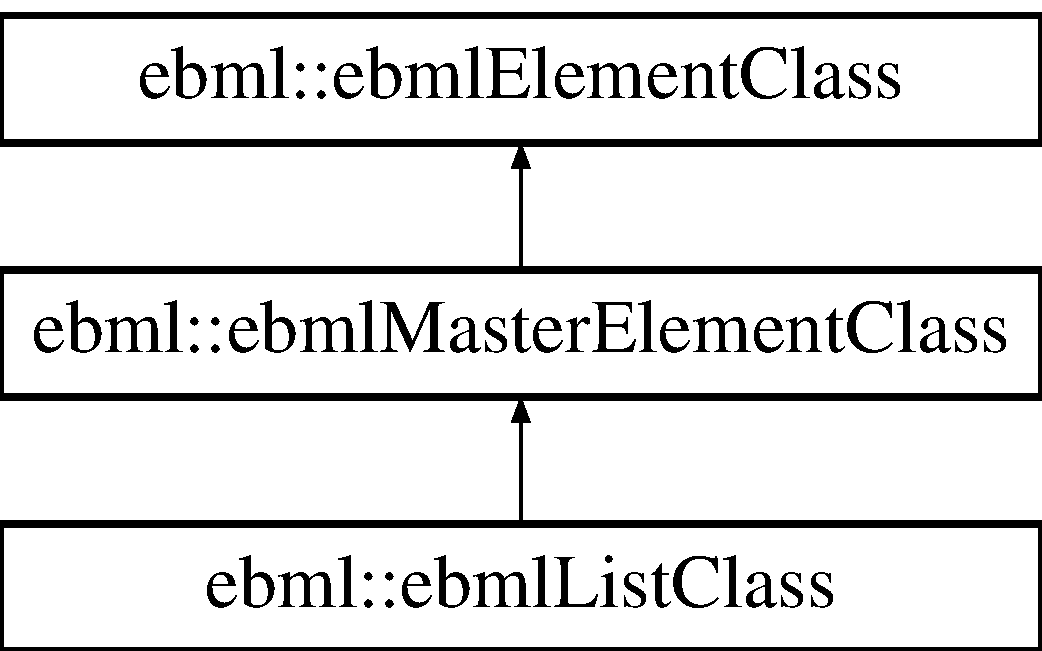
\includegraphics[height=3.000000cm]{classebml_1_1ebmlListClass}
\end{center}
\end{figure}
\subsection*{Public Member Functions}
\begin{DoxyCompactItemize}
\item 
\mbox{\hyperlink{classebml_1_1ebmlListClass_ad49d85790f5d2b18dabf6180895f001d}{ebml\+List\+Class}} (const char $\ast$, const std\+::wstring \&, const \mbox{\hyperlink{structebml_1_1occurSpec__t}{occur\+Spec\+\_\+t}} \&recursive=\{0, 0\})
\item 
\mbox{\hyperlink{classebml_1_1ebmlListClass_afc3e7e9c4a9f663044a77793c20d67ca}{ebml\+List\+Class}} (const char $\ast$, const std\+::wstring \&, const \mbox{\hyperlink{namespaceebml_abf07998998c284c9be3f76b5d9e192e1}{child\+Class\+Spec\+Arg\+\_\+l}} \&, const \mbox{\hyperlink{structebml_1_1occurSpec__t}{occur\+Spec\+\_\+t}} \&recursive=\{0, 0\})
\item 
\mbox{\hyperlink{classebml_1_1ebmlListClass_a8a53119a28cbc5a56b16d3ddc0822116}{ebml\+List\+Class}} (const char $\ast$, const std\+::wstring \&, \mbox{\hyperlink{namespaceebml_a40cf7ad4b58caaa8c07da3ed83f7a431}{child\+Class\+Spec\+Arg\+\_\+init\+\_\+l}}, const \mbox{\hyperlink{structebml_1_1occurSpec__t}{occur\+Spec\+\_\+t}} \&recursive=\{0, 0\})
\item 
\mbox{\hyperlink{classebml_1_1ebmlListClass_ae4f1d932d3b0ba6db79b7fd43f4b9035}{ebml\+List\+Class}} (\mbox{\hyperlink{namespaceebml_a86c5f604ddf12a74aa9812e997a58691}{ebml\+I\+D\+\_\+t}}, const std\+::wstring \&, const \mbox{\hyperlink{structebml_1_1occurSpec__t}{occur\+Spec\+\_\+t}} \&recursive=\{0, 0\})
\item 
\mbox{\hyperlink{classebml_1_1ebmlListClass_a25897c22d3fdc3bf7c4f5751cabf57b6}{ebml\+List\+Class}} (\mbox{\hyperlink{namespaceebml_a86c5f604ddf12a74aa9812e997a58691}{ebml\+I\+D\+\_\+t}}, const std\+::wstring \&, const \mbox{\hyperlink{namespaceebml_abf07998998c284c9be3f76b5d9e192e1}{child\+Class\+Spec\+Arg\+\_\+l}} \&, const \mbox{\hyperlink{structebml_1_1occurSpec__t}{occur\+Spec\+\_\+t}} \&recursive=\{0, 0\})
\item 
\mbox{\hyperlink{classebml_1_1ebmlListClass_ab4ab60f7ad49e7728568920530d32dff}{ebml\+List\+Class}} (\mbox{\hyperlink{namespaceebml_a86c5f604ddf12a74aa9812e997a58691}{ebml\+I\+D\+\_\+t}}, const std\+::wstring \&, \mbox{\hyperlink{namespaceebml_a40cf7ad4b58caaa8c07da3ed83f7a431}{child\+Class\+Spec\+Arg\+\_\+init\+\_\+l}}, const \mbox{\hyperlink{structebml_1_1occurSpec__t}{occur\+Spec\+\_\+t}} \&recursive=\{0, 0\})
\item 
\mbox{\hyperlink{namespaceebml_adad533b7705a16bb360fe56380c5e7be}{ebml\+Element\+\_\+sp}} \mbox{\hyperlink{classebml_1_1ebmlListClass_a115d07c81b0433aaa0510134dabf0f66}{operator()}} (const \mbox{\hyperlink{namespaceebml_a1ddadd26791f273d851882653b9caf70}{ebml\+Element\+\_\+l}} \&) const
\item 
\mbox{\hyperlink{namespaceebml_adad533b7705a16bb360fe56380c5e7be}{ebml\+Element\+\_\+sp}} \mbox{\hyperlink{classebml_1_1ebmlListClass_a5a52d343c43baa7eeb837fb0ab660c07}{operator()}} (\mbox{\hyperlink{namespaceebml_a1ddadd26791f273d851882653b9caf70}{ebml\+Element\+\_\+l}} \&\&) const
\end{DoxyCompactItemize}
\subsection*{Protected Member Functions}
\begin{DoxyCompactItemize}
\item 
\mbox{\hyperlink{classebml_1_1ebmlElement}{ebml\+Element}} $\ast$ \mbox{\hyperlink{classebml_1_1ebmlListClass_aef729ee70f218de1013c3782c481bffb}{\+\_\+new}} () const
\end{DoxyCompactItemize}
\subsection*{Friends}
\begin{DoxyCompactItemize}
\item 
class \mbox{\hyperlink{classebml_1_1ebmlListClass_af371b14231393d2eef62cb562cdd6e2d}{ebml\+List}}
\end{DoxyCompactItemize}
\subsection*{Additional Inherited Members}


\subsection{Constructor \& Destructor Documentation}
\mbox{\Hypertarget{classebml_1_1ebmlListClass_ad49d85790f5d2b18dabf6180895f001d}\label{classebml_1_1ebmlListClass_ad49d85790f5d2b18dabf6180895f001d}} 
\index{ebml\+::ebml\+List\+Class@{ebml\+::ebml\+List\+Class}!ebml\+List\+Class@{ebml\+List\+Class}}
\index{ebml\+List\+Class@{ebml\+List\+Class}!ebml\+::ebml\+List\+Class@{ebml\+::ebml\+List\+Class}}
\subsubsection{\texorpdfstring{ebml\+List\+Class()}{ebmlListClass()}\hspace{0.1cm}{\footnotesize\ttfamily [1/6]}}
{\footnotesize\ttfamily ebml\+::ebml\+List\+Class\+::ebml\+List\+Class (\begin{DoxyParamCaption}\item[{const char $\ast$}]{,  }\item[{const std\+::wstring \&}]{,  }\item[{const \mbox{\hyperlink{structebml_1_1occurSpec__t}{occur\+Spec\+\_\+t}} \&}]{recursive = {\ttfamily \{0,~0\}} }\end{DoxyParamCaption})}

\mbox{\Hypertarget{classebml_1_1ebmlListClass_afc3e7e9c4a9f663044a77793c20d67ca}\label{classebml_1_1ebmlListClass_afc3e7e9c4a9f663044a77793c20d67ca}} 
\index{ebml\+::ebml\+List\+Class@{ebml\+::ebml\+List\+Class}!ebml\+List\+Class@{ebml\+List\+Class}}
\index{ebml\+List\+Class@{ebml\+List\+Class}!ebml\+::ebml\+List\+Class@{ebml\+::ebml\+List\+Class}}
\subsubsection{\texorpdfstring{ebml\+List\+Class()}{ebmlListClass()}\hspace{0.1cm}{\footnotesize\ttfamily [2/6]}}
{\footnotesize\ttfamily ebml\+::ebml\+List\+Class\+::ebml\+List\+Class (\begin{DoxyParamCaption}\item[{const char $\ast$}]{,  }\item[{const std\+::wstring \&}]{,  }\item[{const \mbox{\hyperlink{namespaceebml_abf07998998c284c9be3f76b5d9e192e1}{child\+Class\+Spec\+Arg\+\_\+l}} \&}]{,  }\item[{const \mbox{\hyperlink{structebml_1_1occurSpec__t}{occur\+Spec\+\_\+t}} \&}]{recursive = {\ttfamily \{0,~0\}} }\end{DoxyParamCaption})}

\mbox{\Hypertarget{classebml_1_1ebmlListClass_a8a53119a28cbc5a56b16d3ddc0822116}\label{classebml_1_1ebmlListClass_a8a53119a28cbc5a56b16d3ddc0822116}} 
\index{ebml\+::ebml\+List\+Class@{ebml\+::ebml\+List\+Class}!ebml\+List\+Class@{ebml\+List\+Class}}
\index{ebml\+List\+Class@{ebml\+List\+Class}!ebml\+::ebml\+List\+Class@{ebml\+::ebml\+List\+Class}}
\subsubsection{\texorpdfstring{ebml\+List\+Class()}{ebmlListClass()}\hspace{0.1cm}{\footnotesize\ttfamily [3/6]}}
{\footnotesize\ttfamily ebml\+::ebml\+List\+Class\+::ebml\+List\+Class (\begin{DoxyParamCaption}\item[{const char $\ast$}]{,  }\item[{const std\+::wstring \&}]{,  }\item[{\mbox{\hyperlink{namespaceebml_a40cf7ad4b58caaa8c07da3ed83f7a431}{child\+Class\+Spec\+Arg\+\_\+init\+\_\+l}}}]{,  }\item[{const \mbox{\hyperlink{structebml_1_1occurSpec__t}{occur\+Spec\+\_\+t}} \&}]{recursive = {\ttfamily \{0,~0\}} }\end{DoxyParamCaption})}

\mbox{\Hypertarget{classebml_1_1ebmlListClass_ae4f1d932d3b0ba6db79b7fd43f4b9035}\label{classebml_1_1ebmlListClass_ae4f1d932d3b0ba6db79b7fd43f4b9035}} 
\index{ebml\+::ebml\+List\+Class@{ebml\+::ebml\+List\+Class}!ebml\+List\+Class@{ebml\+List\+Class}}
\index{ebml\+List\+Class@{ebml\+List\+Class}!ebml\+::ebml\+List\+Class@{ebml\+::ebml\+List\+Class}}
\subsubsection{\texorpdfstring{ebml\+List\+Class()}{ebmlListClass()}\hspace{0.1cm}{\footnotesize\ttfamily [4/6]}}
{\footnotesize\ttfamily ebml\+::ebml\+List\+Class\+::ebml\+List\+Class (\begin{DoxyParamCaption}\item[{\mbox{\hyperlink{namespaceebml_a86c5f604ddf12a74aa9812e997a58691}{ebml\+I\+D\+\_\+t}}}]{,  }\item[{const std\+::wstring \&}]{,  }\item[{const \mbox{\hyperlink{structebml_1_1occurSpec__t}{occur\+Spec\+\_\+t}} \&}]{recursive = {\ttfamily \{0,~0\}} }\end{DoxyParamCaption})}

\mbox{\Hypertarget{classebml_1_1ebmlListClass_a25897c22d3fdc3bf7c4f5751cabf57b6}\label{classebml_1_1ebmlListClass_a25897c22d3fdc3bf7c4f5751cabf57b6}} 
\index{ebml\+::ebml\+List\+Class@{ebml\+::ebml\+List\+Class}!ebml\+List\+Class@{ebml\+List\+Class}}
\index{ebml\+List\+Class@{ebml\+List\+Class}!ebml\+::ebml\+List\+Class@{ebml\+::ebml\+List\+Class}}
\subsubsection{\texorpdfstring{ebml\+List\+Class()}{ebmlListClass()}\hspace{0.1cm}{\footnotesize\ttfamily [5/6]}}
{\footnotesize\ttfamily ebml\+::ebml\+List\+Class\+::ebml\+List\+Class (\begin{DoxyParamCaption}\item[{\mbox{\hyperlink{namespaceebml_a86c5f604ddf12a74aa9812e997a58691}{ebml\+I\+D\+\_\+t}}}]{,  }\item[{const std\+::wstring \&}]{,  }\item[{const \mbox{\hyperlink{namespaceebml_abf07998998c284c9be3f76b5d9e192e1}{child\+Class\+Spec\+Arg\+\_\+l}} \&}]{,  }\item[{const \mbox{\hyperlink{structebml_1_1occurSpec__t}{occur\+Spec\+\_\+t}} \&}]{recursive = {\ttfamily \{0,~0\}} }\end{DoxyParamCaption})}

\mbox{\Hypertarget{classebml_1_1ebmlListClass_ab4ab60f7ad49e7728568920530d32dff}\label{classebml_1_1ebmlListClass_ab4ab60f7ad49e7728568920530d32dff}} 
\index{ebml\+::ebml\+List\+Class@{ebml\+::ebml\+List\+Class}!ebml\+List\+Class@{ebml\+List\+Class}}
\index{ebml\+List\+Class@{ebml\+List\+Class}!ebml\+::ebml\+List\+Class@{ebml\+::ebml\+List\+Class}}
\subsubsection{\texorpdfstring{ebml\+List\+Class()}{ebmlListClass()}\hspace{0.1cm}{\footnotesize\ttfamily [6/6]}}
{\footnotesize\ttfamily ebml\+::ebml\+List\+Class\+::ebml\+List\+Class (\begin{DoxyParamCaption}\item[{\mbox{\hyperlink{namespaceebml_a86c5f604ddf12a74aa9812e997a58691}{ebml\+I\+D\+\_\+t}}}]{,  }\item[{const std\+::wstring \&}]{,  }\item[{\mbox{\hyperlink{namespaceebml_a40cf7ad4b58caaa8c07da3ed83f7a431}{child\+Class\+Spec\+Arg\+\_\+init\+\_\+l}}}]{,  }\item[{const \mbox{\hyperlink{structebml_1_1occurSpec__t}{occur\+Spec\+\_\+t}} \&}]{recursive = {\ttfamily \{0,~0\}} }\end{DoxyParamCaption})}



\subsection{Member Function Documentation}
\mbox{\Hypertarget{classebml_1_1ebmlListClass_aef729ee70f218de1013c3782c481bffb}\label{classebml_1_1ebmlListClass_aef729ee70f218de1013c3782c481bffb}} 
\index{ebml\+::ebml\+List\+Class@{ebml\+::ebml\+List\+Class}!\+\_\+new@{\+\_\+new}}
\index{\+\_\+new@{\+\_\+new}!ebml\+::ebml\+List\+Class@{ebml\+::ebml\+List\+Class}}
\subsubsection{\texorpdfstring{\+\_\+new()}{\_new()}}
{\footnotesize\ttfamily \mbox{\hyperlink{classebml_1_1ebmlElement}{ebml\+Element}}$\ast$ ebml\+::ebml\+List\+Class\+::\+\_\+new (\begin{DoxyParamCaption}{ }\end{DoxyParamCaption}) const\hspace{0.3cm}{\ttfamily [protected]}, {\ttfamily [virtual]}}



Implements \mbox{\hyperlink{classebml_1_1ebmlElementClass_a223ede6b8bc3c85251d2d73f0256fb45}{ebml\+::ebml\+Element\+Class}}.

\mbox{\Hypertarget{classebml_1_1ebmlListClass_a115d07c81b0433aaa0510134dabf0f66}\label{classebml_1_1ebmlListClass_a115d07c81b0433aaa0510134dabf0f66}} 
\index{ebml\+::ebml\+List\+Class@{ebml\+::ebml\+List\+Class}!operator()@{operator()}}
\index{operator()@{operator()}!ebml\+::ebml\+List\+Class@{ebml\+::ebml\+List\+Class}}
\subsubsection{\texorpdfstring{operator()()}{operator()()}\hspace{0.1cm}{\footnotesize\ttfamily [1/2]}}
{\footnotesize\ttfamily \mbox{\hyperlink{namespaceebml_adad533b7705a16bb360fe56380c5e7be}{ebml\+Element\+\_\+sp}} ebml\+::ebml\+List\+Class\+::operator() (\begin{DoxyParamCaption}\item[{const \mbox{\hyperlink{namespaceebml_a1ddadd26791f273d851882653b9caf70}{ebml\+Element\+\_\+l}} \&}]{ }\end{DoxyParamCaption}) const}

\mbox{\Hypertarget{classebml_1_1ebmlListClass_a5a52d343c43baa7eeb837fb0ab660c07}\label{classebml_1_1ebmlListClass_a5a52d343c43baa7eeb837fb0ab660c07}} 
\index{ebml\+::ebml\+List\+Class@{ebml\+::ebml\+List\+Class}!operator()@{operator()}}
\index{operator()@{operator()}!ebml\+::ebml\+List\+Class@{ebml\+::ebml\+List\+Class}}
\subsubsection{\texorpdfstring{operator()()}{operator()()}\hspace{0.1cm}{\footnotesize\ttfamily [2/2]}}
{\footnotesize\ttfamily \mbox{\hyperlink{namespaceebml_adad533b7705a16bb360fe56380c5e7be}{ebml\+Element\+\_\+sp}} ebml\+::ebml\+List\+Class\+::operator() (\begin{DoxyParamCaption}\item[{\mbox{\hyperlink{namespaceebml_a1ddadd26791f273d851882653b9caf70}{ebml\+Element\+\_\+l}} \&\&}]{ }\end{DoxyParamCaption}) const}



\subsection{Friends And Related Function Documentation}
\mbox{\Hypertarget{classebml_1_1ebmlListClass_af371b14231393d2eef62cb562cdd6e2d}\label{classebml_1_1ebmlListClass_af371b14231393d2eef62cb562cdd6e2d}} 
\index{ebml\+::ebml\+List\+Class@{ebml\+::ebml\+List\+Class}!ebml\+List@{ebml\+List}}
\index{ebml\+List@{ebml\+List}!ebml\+::ebml\+List\+Class@{ebml\+::ebml\+List\+Class}}
\subsubsection{\texorpdfstring{ebml\+List}{ebmlList}}
{\footnotesize\ttfamily friend class \mbox{\hyperlink{classebml_1_1ebmlList}{ebml\+List}}\hspace{0.3cm}{\ttfamily [friend]}}



The documentation for this class was generated from the following file\+:\begin{DoxyCompactItemize}
\item 
include/libebml\+\_\+ng/masterelement/\mbox{\hyperlink{list_8h}{list.\+h}}\end{DoxyCompactItemize}

\hypertarget{classebml_1_1ebmlMap}{}\section{ebml\+:\+:ebml\+Map$<$ K, H, E, A $>$ Class Template Reference}
\label{classebml_1_1ebmlMap}\index{ebml\+::ebml\+Map$<$ K, H, E, A $>$@{ebml\+::ebml\+Map$<$ K, H, E, A $>$}}


{\ttfamily \#include $<$map.\+h$>$}

Inheritance diagram for ebml\+:\+:ebml\+Map$<$ K, H, E, A $>$\+:\begin{figure}[H]
\begin{center}
\leavevmode
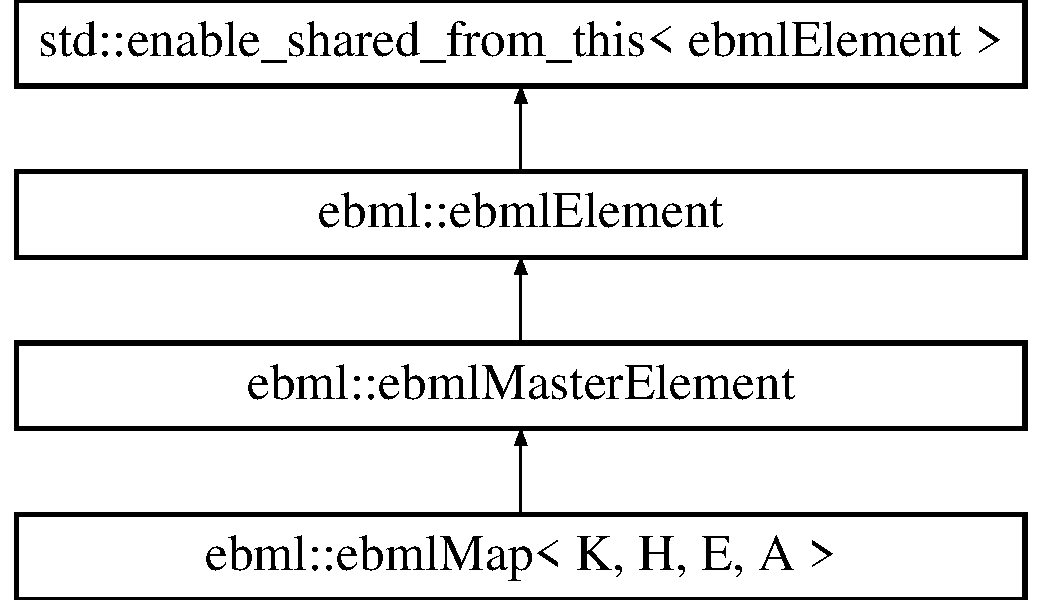
\includegraphics[height=4.000000cm]{classebml_1_1ebmlMap}
\end{center}
\end{figure}
\subsection*{Classes}
\begin{DoxyCompactItemize}
\item 
class \mbox{\hyperlink{classebml_1_1ebmlMap_1_1__const__iterator}{\+\_\+const\+\_\+iterator}}
\item 
class \mbox{\hyperlink{classebml_1_1ebmlMap_1_1__iterator}{\+\_\+iterator}}
\end{DoxyCompactItemize}
\subsection*{Public Member Functions}
\begin{DoxyCompactItemize}
\item 
void \mbox{\hyperlink{classebml_1_1ebmlMap_a1d95a8dbda99fb485977f18f0e5ed992}{set\+Data}} (std\+::initializer\+\_\+list$<$ \mbox{\hyperlink{namespaceebml_adad533b7705a16bb360fe56380c5e7be}{ebml\+Element\+\_\+sp}} $>$)
\item 
void \mbox{\hyperlink{classebml_1_1ebmlMap_a0e78920596118890009d9127f0a42c0e}{set\+Data}} (std\+::initializer\+\_\+list$<$ std\+::pair$<$ \mbox{\hyperlink{namespaceebml_adad533b7705a16bb360fe56380c5e7be}{ebml\+Element\+\_\+sp}}, \mbox{\hyperlink{namespaceebml_adad533b7705a16bb360fe56380c5e7be}{ebml\+Element\+\_\+sp}} $>$$>$)
\item 
void \mbox{\hyperlink{classebml_1_1ebmlMap_ae05e1f77c6d1feed3bf2ff874caf1dba}{set\+Data}} (std\+::initializer\+\_\+list$<$ std\+::pair$<$ K, \mbox{\hyperlink{namespaceebml_adad533b7705a16bb360fe56380c5e7be}{ebml\+Element\+\_\+sp}} $>$$>$)
\item 
void \mbox{\hyperlink{classebml_1_1ebmlMap_aee0f35c791ed14dee89d6e81f47ce58e}{set\+Data}} (const std\+::list$<$ \mbox{\hyperlink{namespaceebml_adad533b7705a16bb360fe56380c5e7be}{ebml\+Element\+\_\+sp}} $>$ \&)
\item 
void \mbox{\hyperlink{classebml_1_1ebmlMap_af3dc95ad8188d5f66235dc58ce304251}{set\+Data}} (const std\+::list$<$ std\+::pair$<$ \mbox{\hyperlink{namespaceebml_adad533b7705a16bb360fe56380c5e7be}{ebml\+Element\+\_\+sp}}, \mbox{\hyperlink{namespaceebml_adad533b7705a16bb360fe56380c5e7be}{ebml\+Element\+\_\+sp}} $>$$>$ \&)
\item 
void \mbox{\hyperlink{classebml_1_1ebmlMap_ae3174082f9f1036e040ce94fa7a85ebd}{set\+Data}} (const std\+::list$<$ std\+::pair$<$ K, \mbox{\hyperlink{namespaceebml_adad533b7705a16bb360fe56380c5e7be}{ebml\+Element\+\_\+sp}} $>$$>$ \&)
\item 
void \mbox{\hyperlink{classebml_1_1ebmlMap_aa8168bc50460fb4e3cd704d16dcd071e}{set\+Data}} (std\+::list$<$ \mbox{\hyperlink{namespaceebml_adad533b7705a16bb360fe56380c5e7be}{ebml\+Element\+\_\+sp}} $>$ \&\&)
\item 
void \mbox{\hyperlink{classebml_1_1ebmlMap_aa3a6c46cc3c149337ffbbb796574e11d}{set\+Data}} (std\+::list$<$ std\+::pair$<$ \mbox{\hyperlink{namespaceebml_adad533b7705a16bb360fe56380c5e7be}{ebml\+Element\+\_\+sp}}, \mbox{\hyperlink{namespaceebml_adad533b7705a16bb360fe56380c5e7be}{ebml\+Element\+\_\+sp}} $>$$>$ \&\&)
\item 
void \mbox{\hyperlink{classebml_1_1ebmlMap_ac0f6f02863ae22a4c9c6b7fdf9a3f635}{set\+Data}} (std\+::list$<$ std\+::pair$<$ K, \mbox{\hyperlink{namespaceebml_adad533b7705a16bb360fe56380c5e7be}{ebml\+Element\+\_\+sp}} $>$$>$ \&\&)
\item 
void \mbox{\hyperlink{classebml_1_1ebmlMap_a44f4a7d1c8cc2b05be540e70e61cfad3}{set\+Data}} (const std\+::unordered\+\_\+map$<$ K, \mbox{\hyperlink{namespaceebml_adad533b7705a16bb360fe56380c5e7be}{ebml\+Element\+\_\+sp}}, H, E, A $>$ \&)
\item 
void \mbox{\hyperlink{classebml_1_1ebmlMap_a04ad9f91a20cd5c32ca169fc1e6e141c}{set\+Data}} (std\+::unordered\+\_\+map$<$ K, \mbox{\hyperlink{namespaceebml_adad533b7705a16bb360fe56380c5e7be}{ebml\+Element\+\_\+sp}}, H, E, A $>$ \&\&)
\item 
std\+::wstring \mbox{\hyperlink{classebml_1_1ebmlMap_a44366a7b060c58b3fbe4e65c31481efc}{minirepr}} () const override
\item 
const \mbox{\hyperlink{classebml_1_1ebmlMapClass}{ebml\+Map\+Class}}$<$ K, H, E, A $>$ $\ast$ \mbox{\hyperlink{classebml_1_1ebmlMap_a44f835be40d70d8425b8e08fbe0ce77f}{cls}} () const override
\item 
\mbox{\hyperlink{classebml_1_1childSlot__t}{child\+Slot\+\_\+t}} \mbox{\hyperlink{classebml_1_1ebmlMap_aec9056894cff0152fd12b95d17af605b}{operator\mbox{[}$\,$\mbox{]}}} (const K \&)
\item 
\mbox{\hyperlink{classebml_1_1childSlot__t}{child\+Slot\+\_\+t}} \mbox{\hyperlink{classebml_1_1ebmlMap_a0b7124e1c16aa43520e201f42614e70f}{at}} (const K \&)
\item 
std\+::pair$<$ \mbox{\hyperlink{classebml_1_1ebmlMasterElement_1_1iterator}{ebml\+Master\+Element\+::iterator}}, bool $>$ \mbox{\hyperlink{classebml_1_1ebmlMap_a34c5d8ef796df9ea13907cd5d75f33a4}{insert}} (const \mbox{\hyperlink{namespaceebml_adad533b7705a16bb360fe56380c5e7be}{ebml\+Element\+\_\+sp}} \&value)
\item 
std\+::pair$<$ \mbox{\hyperlink{classebml_1_1ebmlMasterElement_1_1iterator}{ebml\+Master\+Element\+::iterator}}, bool $>$ \mbox{\hyperlink{classebml_1_1ebmlMap_a6a0236ad1baa318bbd65ce2b755eb3f9}{insert}} (\mbox{\hyperlink{namespaceebml_adad533b7705a16bb360fe56380c5e7be}{ebml\+Element\+\_\+sp}} \&\&value)
\item 
std\+::pair$<$ \mbox{\hyperlink{classebml_1_1ebmlMasterElement_1_1iterator}{ebml\+Master\+Element\+::iterator}}, bool $>$ \mbox{\hyperlink{classebml_1_1ebmlMap_a2e03c68cc11f716e908fd46ab3db8cdc}{insert}} (const std\+::pair$<$ \mbox{\hyperlink{namespaceebml_adad533b7705a16bb360fe56380c5e7be}{ebml\+Element\+\_\+sp}}, \mbox{\hyperlink{namespaceebml_adad533b7705a16bb360fe56380c5e7be}{ebml\+Element\+\_\+sp}} $>$ \&value)
\item 
std\+::pair$<$ \mbox{\hyperlink{classebml_1_1ebmlMasterElement_1_1iterator}{ebml\+Master\+Element\+::iterator}}, bool $>$ \mbox{\hyperlink{classebml_1_1ebmlMap_add662463f1a41aec4fa22827ac1b7e7a}{insert}} (std\+::pair$<$ \mbox{\hyperlink{namespaceebml_adad533b7705a16bb360fe56380c5e7be}{ebml\+Element\+\_\+sp}}, \mbox{\hyperlink{namespaceebml_adad533b7705a16bb360fe56380c5e7be}{ebml\+Element\+\_\+sp}} $>$ \&\&value)
\item 
std\+::pair$<$ \mbox{\hyperlink{classebml_1_1ebmlMasterElement_1_1iterator}{ebml\+Master\+Element\+::iterator}}, bool $>$ \mbox{\hyperlink{classebml_1_1ebmlMap_a9edbbe7cc8bf2eb2f5a73adaac8ce624}{insert}} (const std\+::pair$<$ K, \mbox{\hyperlink{namespaceebml_adad533b7705a16bb360fe56380c5e7be}{ebml\+Element\+\_\+sp}} $>$ \&value)
\item 
std\+::pair$<$ \mbox{\hyperlink{classebml_1_1ebmlMasterElement_1_1iterator}{ebml\+Master\+Element\+::iterator}}, bool $>$ \mbox{\hyperlink{classebml_1_1ebmlMap_a34252351567bad0ac7b844ee7e51095b}{insert}} (std\+::pair$<$ K, \mbox{\hyperlink{namespaceebml_adad533b7705a16bb360fe56380c5e7be}{ebml\+Element\+\_\+sp}} $>$ \&\&value)
\item 
\mbox{\hyperlink{namespaceebml_a2deef4e8071531b32e3533f1bf978917}{c\+\_\+ebml\+Element\+\_\+sp}} \mbox{\hyperlink{classebml_1_1ebmlMap_a509ec9c5ff36ce6b448f475267b6269e}{at}} (const K \&) const
\item 
\mbox{\hyperlink{namespaceebml_a2deef4e8071531b32e3533f1bf978917}{c\+\_\+ebml\+Element\+\_\+sp}} \mbox{\hyperlink{classebml_1_1ebmlMap_afabb04ac79f0daaf31be77832313a7bc}{key\+At}} (const K \&) const
\end{DoxyCompactItemize}
\subsection*{Protected Member Functions}
\begin{DoxyCompactItemize}
\item 
\mbox{\hyperlink{classebml_1_1ebmlMap_ae96480e040d7541d32abddde92ab2b49}{ebml\+Map}} (const \mbox{\hyperlink{classebml_1_1ebmlMapClass}{ebml\+Map\+Class}}$<$ K, H, E, A $>$ $\ast$)
\item 
void \mbox{\hyperlink{classebml_1_1ebmlMap_a3aaf6a51c0e03d5050bdefc527f9776c}{\+\_\+clear}} () override
\item 
void \mbox{\hyperlink{classebml_1_1ebmlMap_ad3807a61a0aa3934eca4882a40e1bda9}{\+\_\+validate\+Data}} (const std\+::list$<$ \mbox{\hyperlink{namespaceebml_adad533b7705a16bb360fe56380c5e7be}{ebml\+Element\+\_\+sp}} $>$ \&)
\item 
std\+::list$<$ \mbox{\hyperlink{namespaceebml_adad533b7705a16bb360fe56380c5e7be}{ebml\+Element\+\_\+sp}} $>$ \mbox{\hyperlink{classebml_1_1ebmlMap_a7a57cf320540396c8010845aeae6db19}{\+\_\+prepare\+Data}} (const std\+::list$<$ std\+::pair$<$ \mbox{\hyperlink{namespaceebml_adad533b7705a16bb360fe56380c5e7be}{ebml\+Element\+\_\+sp}}, \mbox{\hyperlink{namespaceebml_adad533b7705a16bb360fe56380c5e7be}{ebml\+Element\+\_\+sp}} $>$$>$ \&)
\item 
std\+::list$<$ \mbox{\hyperlink{namespaceebml_adad533b7705a16bb360fe56380c5e7be}{ebml\+Element\+\_\+sp}} $>$ \mbox{\hyperlink{classebml_1_1ebmlMap_a52dfd52eeeb589a90de98b7aad3beeef}{\+\_\+prepare\+Data}} (const std\+::list$<$ std\+::pair$<$ K, \mbox{\hyperlink{namespaceebml_adad533b7705a16bb360fe56380c5e7be}{ebml\+Element\+\_\+sp}} $>$$>$ \&)
\item 
std\+::list$<$ \mbox{\hyperlink{namespaceebml_adad533b7705a16bb360fe56380c5e7be}{ebml\+Element\+\_\+sp}} $>$ \mbox{\hyperlink{classebml_1_1ebmlMap_ad9cbd0499431f6dbe19bcc022624d61f}{\+\_\+prepare\+Data}} (std\+::list$<$ std\+::pair$<$ \mbox{\hyperlink{namespaceebml_adad533b7705a16bb360fe56380c5e7be}{ebml\+Element\+\_\+sp}}, \mbox{\hyperlink{namespaceebml_adad533b7705a16bb360fe56380c5e7be}{ebml\+Element\+\_\+sp}} $>$$>$ \&\&)
\item 
std\+::list$<$ \mbox{\hyperlink{namespaceebml_adad533b7705a16bb360fe56380c5e7be}{ebml\+Element\+\_\+sp}} $>$ \mbox{\hyperlink{classebml_1_1ebmlMap_ad061162f3c9e15b0b93af5e557beca6e}{\+\_\+prepare\+Data}} (std\+::list$<$ std\+::pair$<$ K, \mbox{\hyperlink{namespaceebml_adad533b7705a16bb360fe56380c5e7be}{ebml\+Element\+\_\+sp}} $>$$>$ \&\&)
\item 
std\+::unordered\+\_\+map$<$ K, \mbox{\hyperlink{namespaceebml_adad533b7705a16bb360fe56380c5e7be}{ebml\+Element\+\_\+sp}}, H, E, A $>$ \mbox{\hyperlink{classebml_1_1ebmlMap_a5321d1ef4be520aaee8cf6428686314b}{\+\_\+prepare\+Data}} (const std\+::unordered\+\_\+map$<$ K, \mbox{\hyperlink{namespaceebml_adad533b7705a16bb360fe56380c5e7be}{ebml\+Element\+\_\+sp}}, H, E, A $>$ \&)
\item 
std\+::unordered\+\_\+map$<$ K, \mbox{\hyperlink{namespaceebml_adad533b7705a16bb360fe56380c5e7be}{ebml\+Element\+\_\+sp}}, H, E, A $>$ \mbox{\hyperlink{classebml_1_1ebmlMap_a4b1173caaeed4fc75e729a7bae6d3390}{\+\_\+prepare\+Data}} (std\+::unordered\+\_\+map$<$ K, \mbox{\hyperlink{namespaceebml_adad533b7705a16bb360fe56380c5e7be}{ebml\+Element\+\_\+sp}}, H, E, A $>$ \&\&)
\item 
void \mbox{\hyperlink{classebml_1_1ebmlMap_af49238b045b083e8c47d223ec5eaffd2}{\+\_\+set\+Data}} (const std\+::list$<$ \mbox{\hyperlink{namespaceebml_adad533b7705a16bb360fe56380c5e7be}{ebml\+Element\+\_\+sp}} $>$ \&)
\item 
void \mbox{\hyperlink{classebml_1_1ebmlMap_a9779497bcff6f45ae7081e319155376b}{\+\_\+set\+Data}} (std\+::list$<$ \mbox{\hyperlink{namespaceebml_adad533b7705a16bb360fe56380c5e7be}{ebml\+Element\+\_\+sp}} $>$ \&\&)
\item 
void \mbox{\hyperlink{classebml_1_1ebmlMap_a881bfc53cc7f774c9a3aaf79ee6c9e9b}{\+\_\+set\+Data}} (const std\+::unordered\+\_\+map$<$ K, \mbox{\hyperlink{namespaceebml_adad533b7705a16bb360fe56380c5e7be}{ebml\+Element\+\_\+sp}}, H, E, A $>$ \&)
\item 
void \mbox{\hyperlink{classebml_1_1ebmlMap_a0b394fd2545a526334ab909fdb07b1bd}{\+\_\+set\+Data}} (std\+::unordered\+\_\+map$<$ K, \mbox{\hyperlink{namespaceebml_adad533b7705a16bb360fe56380c5e7be}{ebml\+Element\+\_\+sp}}, H, E, A $>$ \&\&)
\item 
\mbox{\hyperlink{classebml_1_1ebmlMasterElement_1_1__iterator}{ebml\+Master\+Element\+::\+\_\+iterator}} $\ast$ \mbox{\hyperlink{classebml_1_1ebmlMap_a1e395f6d3d365562e5bebc37b3cba8ef}{\+\_\+begin}} () override
\item 
\mbox{\hyperlink{classebml_1_1ebmlMasterElement_1_1__iterator}{ebml\+Master\+Element\+::\+\_\+iterator}} $\ast$ \mbox{\hyperlink{classebml_1_1ebmlMap_a8b6a25187190a26a7988d4bbaf853d78}{\+\_\+end}} () override
\item 
\mbox{\hyperlink{classebml_1_1ebmlMasterElement_1_1__const__iterator}{ebml\+Master\+Element\+::\+\_\+const\+\_\+iterator}} $\ast$ \mbox{\hyperlink{classebml_1_1ebmlMap_aa2f09d5ea0bf736dc32a4f04732fd4ba}{\+\_\+cbegin}} () const override
\item 
\mbox{\hyperlink{classebml_1_1ebmlMasterElement_1_1__const__iterator}{ebml\+Master\+Element\+::\+\_\+const\+\_\+iterator}} $\ast$ \mbox{\hyperlink{classebml_1_1ebmlMap_a2a667c679c5ba26d47d834a42921f988}{\+\_\+cend}} () const override
\item 
void \mbox{\hyperlink{classebml_1_1ebmlMap_a50fa3572f500363282894b7978b29464}{\+\_\+add\+Child}} (const \mbox{\hyperlink{namespaceebml_adad533b7705a16bb360fe56380c5e7be}{ebml\+Element\+\_\+sp}} \&) override
\item 
void \mbox{\hyperlink{classebml_1_1ebmlMap_ad3e1f23ca6bb1633c1982fb2cbabb39e}{\+\_\+add\+Child}} (\mbox{\hyperlink{namespaceebml_adad533b7705a16bb360fe56380c5e7be}{ebml\+Element\+\_\+sp}} \&\&) override
\end{DoxyCompactItemize}
\subsection*{Friends}
\begin{DoxyCompactItemize}
\item 
class \mbox{\hyperlink{classebml_1_1ebmlMap_a07a0de0d7e69f365ddabb5fbb0089698}{ebml\+Map\+Class$<$ K, H, E, A $>$}}
\item 
{\footnotesize template$<$typename T , typename U , typename... Args$>$ }\\std\+::shared\+\_\+ptr$<$ U $>$ \mbox{\hyperlink{classebml_1_1ebmlMap_ace404b6adc012cac5ccd9c03160456e3}{new\+\_\+sp}} (Args... args)
\end{DoxyCompactItemize}
\subsection*{Additional Inherited Members}


\subsection{Constructor \& Destructor Documentation}
\mbox{\Hypertarget{classebml_1_1ebmlMap_ae96480e040d7541d32abddde92ab2b49}\label{classebml_1_1ebmlMap_ae96480e040d7541d32abddde92ab2b49}} 
\index{ebml\+::ebml\+Map@{ebml\+::ebml\+Map}!ebml\+Map@{ebml\+Map}}
\index{ebml\+Map@{ebml\+Map}!ebml\+::ebml\+Map@{ebml\+::ebml\+Map}}
\subsubsection{\texorpdfstring{ebml\+Map()}{ebmlMap()}}
{\footnotesize\ttfamily template$<$typename K , typename H , typename E , typename A $>$ \\
\mbox{\hyperlink{classebml_1_1ebmlMap}{ebml\+::ebml\+Map}}$<$ K, H, E, A $>$\+::\mbox{\hyperlink{classebml_1_1ebmlMap}{ebml\+Map}} (\begin{DoxyParamCaption}\item[{const \mbox{\hyperlink{classebml_1_1ebmlMapClass}{ebml\+Map\+Class}}$<$ K, H, E, A $>$ $\ast$}]{ }\end{DoxyParamCaption})\hspace{0.3cm}{\ttfamily [protected]}}



\subsection{Member Function Documentation}
\mbox{\Hypertarget{classebml_1_1ebmlMap_a50fa3572f500363282894b7978b29464}\label{classebml_1_1ebmlMap_a50fa3572f500363282894b7978b29464}} 
\index{ebml\+::ebml\+Map@{ebml\+::ebml\+Map}!\+\_\+add\+Child@{\+\_\+add\+Child}}
\index{\+\_\+add\+Child@{\+\_\+add\+Child}!ebml\+::ebml\+Map@{ebml\+::ebml\+Map}}
\subsubsection{\texorpdfstring{\+\_\+add\+Child()}{\_addChild()}\hspace{0.1cm}{\footnotesize\ttfamily [1/2]}}
{\footnotesize\ttfamily template$<$typename K , typename H , typename E , typename A $>$ \\
void \mbox{\hyperlink{classebml_1_1ebmlMap}{ebml\+::ebml\+Map}}$<$ K, H, E, A $>$\+::\+\_\+add\+Child (\begin{DoxyParamCaption}\item[{const \mbox{\hyperlink{namespaceebml_adad533b7705a16bb360fe56380c5e7be}{ebml\+Element\+\_\+sp}} \&}]{ }\end{DoxyParamCaption})\hspace{0.3cm}{\ttfamily [override]}, {\ttfamily [protected]}, {\ttfamily [virtual]}}



Implements \mbox{\hyperlink{classebml_1_1ebmlMasterElement_a59c5f3b3409fd5fd6f0f22c7a68f1c9b}{ebml\+::ebml\+Master\+Element}}.

\mbox{\Hypertarget{classebml_1_1ebmlMap_ad3e1f23ca6bb1633c1982fb2cbabb39e}\label{classebml_1_1ebmlMap_ad3e1f23ca6bb1633c1982fb2cbabb39e}} 
\index{ebml\+::ebml\+Map@{ebml\+::ebml\+Map}!\+\_\+add\+Child@{\+\_\+add\+Child}}
\index{\+\_\+add\+Child@{\+\_\+add\+Child}!ebml\+::ebml\+Map@{ebml\+::ebml\+Map}}
\subsubsection{\texorpdfstring{\+\_\+add\+Child()}{\_addChild()}\hspace{0.1cm}{\footnotesize\ttfamily [2/2]}}
{\footnotesize\ttfamily template$<$typename K , typename H , typename E , typename A $>$ \\
void \mbox{\hyperlink{classebml_1_1ebmlMap}{ebml\+::ebml\+Map}}$<$ K, H, E, A $>$\+::\+\_\+add\+Child (\begin{DoxyParamCaption}\item[{\mbox{\hyperlink{namespaceebml_adad533b7705a16bb360fe56380c5e7be}{ebml\+Element\+\_\+sp}} \&\&}]{ }\end{DoxyParamCaption})\hspace{0.3cm}{\ttfamily [override]}, {\ttfamily [protected]}, {\ttfamily [virtual]}}



Implements \mbox{\hyperlink{classebml_1_1ebmlMasterElement_a3af0270846a1ced1719d26dd261f0355}{ebml\+::ebml\+Master\+Element}}.

\mbox{\Hypertarget{classebml_1_1ebmlMap_a1e395f6d3d365562e5bebc37b3cba8ef}\label{classebml_1_1ebmlMap_a1e395f6d3d365562e5bebc37b3cba8ef}} 
\index{ebml\+::ebml\+Map@{ebml\+::ebml\+Map}!\+\_\+begin@{\+\_\+begin}}
\index{\+\_\+begin@{\+\_\+begin}!ebml\+::ebml\+Map@{ebml\+::ebml\+Map}}
\subsubsection{\texorpdfstring{\+\_\+begin()}{\_begin()}}
{\footnotesize\ttfamily template$<$typename K , typename H , typename E , typename A $>$ \\
\mbox{\hyperlink{classebml_1_1ebmlMasterElement_1_1__iterator}{ebml\+Master\+Element\+::\+\_\+iterator}}$\ast$ \mbox{\hyperlink{classebml_1_1ebmlMap}{ebml\+::ebml\+Map}}$<$ K, H, E, A $>$\+::\+\_\+begin (\begin{DoxyParamCaption}{ }\end{DoxyParamCaption})\hspace{0.3cm}{\ttfamily [override]}, {\ttfamily [protected]}, {\ttfamily [virtual]}}



Implements \mbox{\hyperlink{classebml_1_1ebmlMasterElement_af6fb7a9934e9b8d0c64273ef6944f44b}{ebml\+::ebml\+Master\+Element}}.

\mbox{\Hypertarget{classebml_1_1ebmlMap_aa2f09d5ea0bf736dc32a4f04732fd4ba}\label{classebml_1_1ebmlMap_aa2f09d5ea0bf736dc32a4f04732fd4ba}} 
\index{ebml\+::ebml\+Map@{ebml\+::ebml\+Map}!\+\_\+cbegin@{\+\_\+cbegin}}
\index{\+\_\+cbegin@{\+\_\+cbegin}!ebml\+::ebml\+Map@{ebml\+::ebml\+Map}}
\subsubsection{\texorpdfstring{\+\_\+cbegin()}{\_cbegin()}}
{\footnotesize\ttfamily template$<$typename K , typename H , typename E , typename A $>$ \\
\mbox{\hyperlink{classebml_1_1ebmlMasterElement_1_1__const__iterator}{ebml\+Master\+Element\+::\+\_\+const\+\_\+iterator}}$\ast$ \mbox{\hyperlink{classebml_1_1ebmlMap}{ebml\+::ebml\+Map}}$<$ K, H, E, A $>$\+::\+\_\+cbegin (\begin{DoxyParamCaption}{ }\end{DoxyParamCaption}) const\hspace{0.3cm}{\ttfamily [override]}, {\ttfamily [protected]}, {\ttfamily [virtual]}}



Implements \mbox{\hyperlink{classebml_1_1ebmlMasterElement_a7e1ffa498e22b637a6671df14aa0bc45}{ebml\+::ebml\+Master\+Element}}.

\mbox{\Hypertarget{classebml_1_1ebmlMap_a2a667c679c5ba26d47d834a42921f988}\label{classebml_1_1ebmlMap_a2a667c679c5ba26d47d834a42921f988}} 
\index{ebml\+::ebml\+Map@{ebml\+::ebml\+Map}!\+\_\+cend@{\+\_\+cend}}
\index{\+\_\+cend@{\+\_\+cend}!ebml\+::ebml\+Map@{ebml\+::ebml\+Map}}
\subsubsection{\texorpdfstring{\+\_\+cend()}{\_cend()}}
{\footnotesize\ttfamily template$<$typename K , typename H , typename E , typename A $>$ \\
\mbox{\hyperlink{classebml_1_1ebmlMasterElement_1_1__const__iterator}{ebml\+Master\+Element\+::\+\_\+const\+\_\+iterator}}$\ast$ \mbox{\hyperlink{classebml_1_1ebmlMap}{ebml\+::ebml\+Map}}$<$ K, H, E, A $>$\+::\+\_\+cend (\begin{DoxyParamCaption}{ }\end{DoxyParamCaption}) const\hspace{0.3cm}{\ttfamily [override]}, {\ttfamily [protected]}, {\ttfamily [virtual]}}



Implements \mbox{\hyperlink{classebml_1_1ebmlMasterElement_ae6cdbf68d8267a7ab098bd402fa70e88}{ebml\+::ebml\+Master\+Element}}.

\mbox{\Hypertarget{classebml_1_1ebmlMap_a3aaf6a51c0e03d5050bdefc527f9776c}\label{classebml_1_1ebmlMap_a3aaf6a51c0e03d5050bdefc527f9776c}} 
\index{ebml\+::ebml\+Map@{ebml\+::ebml\+Map}!\+\_\+clear@{\+\_\+clear}}
\index{\+\_\+clear@{\+\_\+clear}!ebml\+::ebml\+Map@{ebml\+::ebml\+Map}}
\subsubsection{\texorpdfstring{\+\_\+clear()}{\_clear()}}
{\footnotesize\ttfamily template$<$typename K , typename H , typename E , typename A $>$ \\
void \mbox{\hyperlink{classebml_1_1ebmlMap}{ebml\+::ebml\+Map}}$<$ K, H, E, A $>$\+::\+\_\+clear (\begin{DoxyParamCaption}{ }\end{DoxyParamCaption})\hspace{0.3cm}{\ttfamily [override]}, {\ttfamily [protected]}, {\ttfamily [virtual]}}



Reimplemented from \mbox{\hyperlink{classebml_1_1ebmlMasterElement_a2fdf9fa1022f06a046fe94e631e266a3}{ebml\+::ebml\+Master\+Element}}.

\mbox{\Hypertarget{classebml_1_1ebmlMap_a8b6a25187190a26a7988d4bbaf853d78}\label{classebml_1_1ebmlMap_a8b6a25187190a26a7988d4bbaf853d78}} 
\index{ebml\+::ebml\+Map@{ebml\+::ebml\+Map}!\+\_\+end@{\+\_\+end}}
\index{\+\_\+end@{\+\_\+end}!ebml\+::ebml\+Map@{ebml\+::ebml\+Map}}
\subsubsection{\texorpdfstring{\+\_\+end()}{\_end()}}
{\footnotesize\ttfamily template$<$typename K , typename H , typename E , typename A $>$ \\
\mbox{\hyperlink{classebml_1_1ebmlMasterElement_1_1__iterator}{ebml\+Master\+Element\+::\+\_\+iterator}}$\ast$ \mbox{\hyperlink{classebml_1_1ebmlMap}{ebml\+::ebml\+Map}}$<$ K, H, E, A $>$\+::\+\_\+end (\begin{DoxyParamCaption}{ }\end{DoxyParamCaption})\hspace{0.3cm}{\ttfamily [override]}, {\ttfamily [protected]}, {\ttfamily [virtual]}}



Implements \mbox{\hyperlink{classebml_1_1ebmlMasterElement_a352e5e11836063394990cb05c09d8e48}{ebml\+::ebml\+Master\+Element}}.

\mbox{\Hypertarget{classebml_1_1ebmlMap_a7a57cf320540396c8010845aeae6db19}\label{classebml_1_1ebmlMap_a7a57cf320540396c8010845aeae6db19}} 
\index{ebml\+::ebml\+Map@{ebml\+::ebml\+Map}!\+\_\+prepare\+Data@{\+\_\+prepare\+Data}}
\index{\+\_\+prepare\+Data@{\+\_\+prepare\+Data}!ebml\+::ebml\+Map@{ebml\+::ebml\+Map}}
\subsubsection{\texorpdfstring{\+\_\+prepare\+Data()}{\_prepareData()}\hspace{0.1cm}{\footnotesize\ttfamily [1/6]}}
{\footnotesize\ttfamily template$<$typename K , typename H , typename E , typename A $>$ \\
std\+::list$<$\mbox{\hyperlink{namespaceebml_adad533b7705a16bb360fe56380c5e7be}{ebml\+Element\+\_\+sp}}$>$ \mbox{\hyperlink{classebml_1_1ebmlMap}{ebml\+::ebml\+Map}}$<$ K, H, E, A $>$\+::\+\_\+prepare\+Data (\begin{DoxyParamCaption}\item[{const std\+::list$<$ std\+::pair$<$ \mbox{\hyperlink{namespaceebml_adad533b7705a16bb360fe56380c5e7be}{ebml\+Element\+\_\+sp}}, \mbox{\hyperlink{namespaceebml_adad533b7705a16bb360fe56380c5e7be}{ebml\+Element\+\_\+sp}} $>$$>$ \&}]{ }\end{DoxyParamCaption})\hspace{0.3cm}{\ttfamily [protected]}}

\mbox{\Hypertarget{classebml_1_1ebmlMap_a52dfd52eeeb589a90de98b7aad3beeef}\label{classebml_1_1ebmlMap_a52dfd52eeeb589a90de98b7aad3beeef}} 
\index{ebml\+::ebml\+Map@{ebml\+::ebml\+Map}!\+\_\+prepare\+Data@{\+\_\+prepare\+Data}}
\index{\+\_\+prepare\+Data@{\+\_\+prepare\+Data}!ebml\+::ebml\+Map@{ebml\+::ebml\+Map}}
\subsubsection{\texorpdfstring{\+\_\+prepare\+Data()}{\_prepareData()}\hspace{0.1cm}{\footnotesize\ttfamily [2/6]}}
{\footnotesize\ttfamily template$<$typename K , typename H , typename E , typename A $>$ \\
std\+::list$<$\mbox{\hyperlink{namespaceebml_adad533b7705a16bb360fe56380c5e7be}{ebml\+Element\+\_\+sp}}$>$ \mbox{\hyperlink{classebml_1_1ebmlMap}{ebml\+::ebml\+Map}}$<$ K, H, E, A $>$\+::\+\_\+prepare\+Data (\begin{DoxyParamCaption}\item[{const std\+::list$<$ std\+::pair$<$ K, \mbox{\hyperlink{namespaceebml_adad533b7705a16bb360fe56380c5e7be}{ebml\+Element\+\_\+sp}} $>$$>$ \&}]{ }\end{DoxyParamCaption})\hspace{0.3cm}{\ttfamily [protected]}}

\mbox{\Hypertarget{classebml_1_1ebmlMap_ad9cbd0499431f6dbe19bcc022624d61f}\label{classebml_1_1ebmlMap_ad9cbd0499431f6dbe19bcc022624d61f}} 
\index{ebml\+::ebml\+Map@{ebml\+::ebml\+Map}!\+\_\+prepare\+Data@{\+\_\+prepare\+Data}}
\index{\+\_\+prepare\+Data@{\+\_\+prepare\+Data}!ebml\+::ebml\+Map@{ebml\+::ebml\+Map}}
\subsubsection{\texorpdfstring{\+\_\+prepare\+Data()}{\_prepareData()}\hspace{0.1cm}{\footnotesize\ttfamily [3/6]}}
{\footnotesize\ttfamily template$<$typename K , typename H , typename E , typename A $>$ \\
std\+::list$<$\mbox{\hyperlink{namespaceebml_adad533b7705a16bb360fe56380c5e7be}{ebml\+Element\+\_\+sp}}$>$ \mbox{\hyperlink{classebml_1_1ebmlMap}{ebml\+::ebml\+Map}}$<$ K, H, E, A $>$\+::\+\_\+prepare\+Data (\begin{DoxyParamCaption}\item[{std\+::list$<$ std\+::pair$<$ \mbox{\hyperlink{namespaceebml_adad533b7705a16bb360fe56380c5e7be}{ebml\+Element\+\_\+sp}}, \mbox{\hyperlink{namespaceebml_adad533b7705a16bb360fe56380c5e7be}{ebml\+Element\+\_\+sp}} $>$$>$ \&\&}]{ }\end{DoxyParamCaption})\hspace{0.3cm}{\ttfamily [protected]}}

\mbox{\Hypertarget{classebml_1_1ebmlMap_ad061162f3c9e15b0b93af5e557beca6e}\label{classebml_1_1ebmlMap_ad061162f3c9e15b0b93af5e557beca6e}} 
\index{ebml\+::ebml\+Map@{ebml\+::ebml\+Map}!\+\_\+prepare\+Data@{\+\_\+prepare\+Data}}
\index{\+\_\+prepare\+Data@{\+\_\+prepare\+Data}!ebml\+::ebml\+Map@{ebml\+::ebml\+Map}}
\subsubsection{\texorpdfstring{\+\_\+prepare\+Data()}{\_prepareData()}\hspace{0.1cm}{\footnotesize\ttfamily [4/6]}}
{\footnotesize\ttfamily template$<$typename K , typename H , typename E , typename A $>$ \\
std\+::list$<$\mbox{\hyperlink{namespaceebml_adad533b7705a16bb360fe56380c5e7be}{ebml\+Element\+\_\+sp}}$>$ \mbox{\hyperlink{classebml_1_1ebmlMap}{ebml\+::ebml\+Map}}$<$ K, H, E, A $>$\+::\+\_\+prepare\+Data (\begin{DoxyParamCaption}\item[{std\+::list$<$ std\+::pair$<$ K, \mbox{\hyperlink{namespaceebml_adad533b7705a16bb360fe56380c5e7be}{ebml\+Element\+\_\+sp}} $>$$>$ \&\&}]{ }\end{DoxyParamCaption})\hspace{0.3cm}{\ttfamily [protected]}}

\mbox{\Hypertarget{classebml_1_1ebmlMap_a5321d1ef4be520aaee8cf6428686314b}\label{classebml_1_1ebmlMap_a5321d1ef4be520aaee8cf6428686314b}} 
\index{ebml\+::ebml\+Map@{ebml\+::ebml\+Map}!\+\_\+prepare\+Data@{\+\_\+prepare\+Data}}
\index{\+\_\+prepare\+Data@{\+\_\+prepare\+Data}!ebml\+::ebml\+Map@{ebml\+::ebml\+Map}}
\subsubsection{\texorpdfstring{\+\_\+prepare\+Data()}{\_prepareData()}\hspace{0.1cm}{\footnotesize\ttfamily [5/6]}}
{\footnotesize\ttfamily template$<$typename K , typename H , typename E , typename A $>$ \\
std\+::unordered\+\_\+map$<$K, \mbox{\hyperlink{namespaceebml_adad533b7705a16bb360fe56380c5e7be}{ebml\+Element\+\_\+sp}}, H, E, A$>$ \mbox{\hyperlink{classebml_1_1ebmlMap}{ebml\+::ebml\+Map}}$<$ K, H, E, A $>$\+::\+\_\+prepare\+Data (\begin{DoxyParamCaption}\item[{const std\+::unordered\+\_\+map$<$ K, \mbox{\hyperlink{namespaceebml_adad533b7705a16bb360fe56380c5e7be}{ebml\+Element\+\_\+sp}}, H, E, A $>$ \&}]{ }\end{DoxyParamCaption})\hspace{0.3cm}{\ttfamily [protected]}}

\mbox{\Hypertarget{classebml_1_1ebmlMap_a4b1173caaeed4fc75e729a7bae6d3390}\label{classebml_1_1ebmlMap_a4b1173caaeed4fc75e729a7bae6d3390}} 
\index{ebml\+::ebml\+Map@{ebml\+::ebml\+Map}!\+\_\+prepare\+Data@{\+\_\+prepare\+Data}}
\index{\+\_\+prepare\+Data@{\+\_\+prepare\+Data}!ebml\+::ebml\+Map@{ebml\+::ebml\+Map}}
\subsubsection{\texorpdfstring{\+\_\+prepare\+Data()}{\_prepareData()}\hspace{0.1cm}{\footnotesize\ttfamily [6/6]}}
{\footnotesize\ttfamily template$<$typename K , typename H , typename E , typename A $>$ \\
std\+::unordered\+\_\+map$<$K, \mbox{\hyperlink{namespaceebml_adad533b7705a16bb360fe56380c5e7be}{ebml\+Element\+\_\+sp}}, H, E, A$>$ \mbox{\hyperlink{classebml_1_1ebmlMap}{ebml\+::ebml\+Map}}$<$ K, H, E, A $>$\+::\+\_\+prepare\+Data (\begin{DoxyParamCaption}\item[{std\+::unordered\+\_\+map$<$ K, \mbox{\hyperlink{namespaceebml_adad533b7705a16bb360fe56380c5e7be}{ebml\+Element\+\_\+sp}}, H, E, A $>$ \&\&}]{ }\end{DoxyParamCaption})\hspace{0.3cm}{\ttfamily [protected]}}

\mbox{\Hypertarget{classebml_1_1ebmlMap_af49238b045b083e8c47d223ec5eaffd2}\label{classebml_1_1ebmlMap_af49238b045b083e8c47d223ec5eaffd2}} 
\index{ebml\+::ebml\+Map@{ebml\+::ebml\+Map}!\+\_\+set\+Data@{\+\_\+set\+Data}}
\index{\+\_\+set\+Data@{\+\_\+set\+Data}!ebml\+::ebml\+Map@{ebml\+::ebml\+Map}}
\subsubsection{\texorpdfstring{\+\_\+set\+Data()}{\_setData()}\hspace{0.1cm}{\footnotesize\ttfamily [1/4]}}
{\footnotesize\ttfamily template$<$typename K , typename H , typename E , typename A $>$ \\
void \mbox{\hyperlink{classebml_1_1ebmlMap}{ebml\+::ebml\+Map}}$<$ K, H, E, A $>$\+::\+\_\+set\+Data (\begin{DoxyParamCaption}\item[{const std\+::list$<$ \mbox{\hyperlink{namespaceebml_adad533b7705a16bb360fe56380c5e7be}{ebml\+Element\+\_\+sp}} $>$ \&}]{ }\end{DoxyParamCaption})\hspace{0.3cm}{\ttfamily [protected]}}

\mbox{\Hypertarget{classebml_1_1ebmlMap_a9779497bcff6f45ae7081e319155376b}\label{classebml_1_1ebmlMap_a9779497bcff6f45ae7081e319155376b}} 
\index{ebml\+::ebml\+Map@{ebml\+::ebml\+Map}!\+\_\+set\+Data@{\+\_\+set\+Data}}
\index{\+\_\+set\+Data@{\+\_\+set\+Data}!ebml\+::ebml\+Map@{ebml\+::ebml\+Map}}
\subsubsection{\texorpdfstring{\+\_\+set\+Data()}{\_setData()}\hspace{0.1cm}{\footnotesize\ttfamily [2/4]}}
{\footnotesize\ttfamily template$<$typename K , typename H , typename E , typename A $>$ \\
void \mbox{\hyperlink{classebml_1_1ebmlMap}{ebml\+::ebml\+Map}}$<$ K, H, E, A $>$\+::\+\_\+set\+Data (\begin{DoxyParamCaption}\item[{std\+::list$<$ \mbox{\hyperlink{namespaceebml_adad533b7705a16bb360fe56380c5e7be}{ebml\+Element\+\_\+sp}} $>$ \&\&}]{ }\end{DoxyParamCaption})\hspace{0.3cm}{\ttfamily [protected]}}

\mbox{\Hypertarget{classebml_1_1ebmlMap_a881bfc53cc7f774c9a3aaf79ee6c9e9b}\label{classebml_1_1ebmlMap_a881bfc53cc7f774c9a3aaf79ee6c9e9b}} 
\index{ebml\+::ebml\+Map@{ebml\+::ebml\+Map}!\+\_\+set\+Data@{\+\_\+set\+Data}}
\index{\+\_\+set\+Data@{\+\_\+set\+Data}!ebml\+::ebml\+Map@{ebml\+::ebml\+Map}}
\subsubsection{\texorpdfstring{\+\_\+set\+Data()}{\_setData()}\hspace{0.1cm}{\footnotesize\ttfamily [3/4]}}
{\footnotesize\ttfamily template$<$typename K , typename H , typename E , typename A $>$ \\
void \mbox{\hyperlink{classebml_1_1ebmlMap}{ebml\+::ebml\+Map}}$<$ K, H, E, A $>$\+::\+\_\+set\+Data (\begin{DoxyParamCaption}\item[{const std\+::unordered\+\_\+map$<$ K, \mbox{\hyperlink{namespaceebml_adad533b7705a16bb360fe56380c5e7be}{ebml\+Element\+\_\+sp}}, H, E, A $>$ \&}]{ }\end{DoxyParamCaption})\hspace{0.3cm}{\ttfamily [protected]}}

\mbox{\Hypertarget{classebml_1_1ebmlMap_a0b394fd2545a526334ab909fdb07b1bd}\label{classebml_1_1ebmlMap_a0b394fd2545a526334ab909fdb07b1bd}} 
\index{ebml\+::ebml\+Map@{ebml\+::ebml\+Map}!\+\_\+set\+Data@{\+\_\+set\+Data}}
\index{\+\_\+set\+Data@{\+\_\+set\+Data}!ebml\+::ebml\+Map@{ebml\+::ebml\+Map}}
\subsubsection{\texorpdfstring{\+\_\+set\+Data()}{\_setData()}\hspace{0.1cm}{\footnotesize\ttfamily [4/4]}}
{\footnotesize\ttfamily template$<$typename K , typename H , typename E , typename A $>$ \\
void \mbox{\hyperlink{classebml_1_1ebmlMap}{ebml\+::ebml\+Map}}$<$ K, H, E, A $>$\+::\+\_\+set\+Data (\begin{DoxyParamCaption}\item[{std\+::unordered\+\_\+map$<$ K, \mbox{\hyperlink{namespaceebml_adad533b7705a16bb360fe56380c5e7be}{ebml\+Element\+\_\+sp}}, H, E, A $>$ \&\&}]{ }\end{DoxyParamCaption})\hspace{0.3cm}{\ttfamily [protected]}}

\mbox{\Hypertarget{classebml_1_1ebmlMap_ad3807a61a0aa3934eca4882a40e1bda9}\label{classebml_1_1ebmlMap_ad3807a61a0aa3934eca4882a40e1bda9}} 
\index{ebml\+::ebml\+Map@{ebml\+::ebml\+Map}!\+\_\+validate\+Data@{\+\_\+validate\+Data}}
\index{\+\_\+validate\+Data@{\+\_\+validate\+Data}!ebml\+::ebml\+Map@{ebml\+::ebml\+Map}}
\subsubsection{\texorpdfstring{\+\_\+validate\+Data()}{\_validateData()}}
{\footnotesize\ttfamily template$<$typename K , typename H , typename E , typename A $>$ \\
void \mbox{\hyperlink{classebml_1_1ebmlMap}{ebml\+::ebml\+Map}}$<$ K, H, E, A $>$\+::\+\_\+validate\+Data (\begin{DoxyParamCaption}\item[{const std\+::list$<$ \mbox{\hyperlink{namespaceebml_adad533b7705a16bb360fe56380c5e7be}{ebml\+Element\+\_\+sp}} $>$ \&}]{ }\end{DoxyParamCaption})\hspace{0.3cm}{\ttfamily [protected]}}

\mbox{\Hypertarget{classebml_1_1ebmlMap_a0b7124e1c16aa43520e201f42614e70f}\label{classebml_1_1ebmlMap_a0b7124e1c16aa43520e201f42614e70f}} 
\index{ebml\+::ebml\+Map@{ebml\+::ebml\+Map}!at@{at}}
\index{at@{at}!ebml\+::ebml\+Map@{ebml\+::ebml\+Map}}
\subsubsection{\texorpdfstring{at()}{at()}\hspace{0.1cm}{\footnotesize\ttfamily [1/2]}}
{\footnotesize\ttfamily template$<$typename K , typename H , typename E , typename A $>$ \\
\mbox{\hyperlink{classebml_1_1childSlot__t}{child\+Slot\+\_\+t}} \mbox{\hyperlink{classebml_1_1ebmlMap}{ebml\+::ebml\+Map}}$<$ K, H, E, A $>$\+::at (\begin{DoxyParamCaption}\item[{const K \&}]{ }\end{DoxyParamCaption})}

\mbox{\Hypertarget{classebml_1_1ebmlMap_a509ec9c5ff36ce6b448f475267b6269e}\label{classebml_1_1ebmlMap_a509ec9c5ff36ce6b448f475267b6269e}} 
\index{ebml\+::ebml\+Map@{ebml\+::ebml\+Map}!at@{at}}
\index{at@{at}!ebml\+::ebml\+Map@{ebml\+::ebml\+Map}}
\subsubsection{\texorpdfstring{at()}{at()}\hspace{0.1cm}{\footnotesize\ttfamily [2/2]}}
{\footnotesize\ttfamily template$<$typename K , typename H , typename E , typename A $>$ \\
\mbox{\hyperlink{namespaceebml_a2deef4e8071531b32e3533f1bf978917}{c\+\_\+ebml\+Element\+\_\+sp}} \mbox{\hyperlink{classebml_1_1ebmlMap}{ebml\+::ebml\+Map}}$<$ K, H, E, A $>$\+::at (\begin{DoxyParamCaption}\item[{const K \&}]{ }\end{DoxyParamCaption}) const}

\mbox{\Hypertarget{classebml_1_1ebmlMap_a44f835be40d70d8425b8e08fbe0ce77f}\label{classebml_1_1ebmlMap_a44f835be40d70d8425b8e08fbe0ce77f}} 
\index{ebml\+::ebml\+Map@{ebml\+::ebml\+Map}!cls@{cls}}
\index{cls@{cls}!ebml\+::ebml\+Map@{ebml\+::ebml\+Map}}
\subsubsection{\texorpdfstring{cls()}{cls()}}
{\footnotesize\ttfamily template$<$typename K , typename H , typename E , typename A $>$ \\
const \mbox{\hyperlink{classebml_1_1ebmlMapClass}{ebml\+Map\+Class}}$<$K, H, E, A$>$$\ast$ \mbox{\hyperlink{classebml_1_1ebmlMap}{ebml\+::ebml\+Map}}$<$ K, H, E, A $>$\+::cls (\begin{DoxyParamCaption}{ }\end{DoxyParamCaption}) const\hspace{0.3cm}{\ttfamily [override]}, {\ttfamily [virtual]}}



Reimplemented from \mbox{\hyperlink{classebml_1_1ebmlMasterElement_a4073fb3f7ce3dda153384821714df29e}{ebml\+::ebml\+Master\+Element}}.

\mbox{\Hypertarget{classebml_1_1ebmlMap_a34c5d8ef796df9ea13907cd5d75f33a4}\label{classebml_1_1ebmlMap_a34c5d8ef796df9ea13907cd5d75f33a4}} 
\index{ebml\+::ebml\+Map@{ebml\+::ebml\+Map}!insert@{insert}}
\index{insert@{insert}!ebml\+::ebml\+Map@{ebml\+::ebml\+Map}}
\subsubsection{\texorpdfstring{insert()}{insert()}\hspace{0.1cm}{\footnotesize\ttfamily [1/6]}}
{\footnotesize\ttfamily template$<$typename K , typename H , typename E , typename A $>$ \\
std\+::pair$<$\mbox{\hyperlink{classebml_1_1ebmlMasterElement_1_1iterator}{ebml\+Master\+Element\+::iterator}}, bool$>$ \mbox{\hyperlink{classebml_1_1ebmlMap}{ebml\+::ebml\+Map}}$<$ K, H, E, A $>$\+::insert (\begin{DoxyParamCaption}\item[{const \mbox{\hyperlink{namespaceebml_adad533b7705a16bb360fe56380c5e7be}{ebml\+Element\+\_\+sp}} \&}]{value }\end{DoxyParamCaption})}

\mbox{\Hypertarget{classebml_1_1ebmlMap_a6a0236ad1baa318bbd65ce2b755eb3f9}\label{classebml_1_1ebmlMap_a6a0236ad1baa318bbd65ce2b755eb3f9}} 
\index{ebml\+::ebml\+Map@{ebml\+::ebml\+Map}!insert@{insert}}
\index{insert@{insert}!ebml\+::ebml\+Map@{ebml\+::ebml\+Map}}
\subsubsection{\texorpdfstring{insert()}{insert()}\hspace{0.1cm}{\footnotesize\ttfamily [2/6]}}
{\footnotesize\ttfamily template$<$typename K , typename H , typename E , typename A $>$ \\
std\+::pair$<$\mbox{\hyperlink{classebml_1_1ebmlMasterElement_1_1iterator}{ebml\+Master\+Element\+::iterator}}, bool$>$ \mbox{\hyperlink{classebml_1_1ebmlMap}{ebml\+::ebml\+Map}}$<$ K, H, E, A $>$\+::insert (\begin{DoxyParamCaption}\item[{\mbox{\hyperlink{namespaceebml_adad533b7705a16bb360fe56380c5e7be}{ebml\+Element\+\_\+sp}} \&\&}]{value }\end{DoxyParamCaption})}

\mbox{\Hypertarget{classebml_1_1ebmlMap_a2e03c68cc11f716e908fd46ab3db8cdc}\label{classebml_1_1ebmlMap_a2e03c68cc11f716e908fd46ab3db8cdc}} 
\index{ebml\+::ebml\+Map@{ebml\+::ebml\+Map}!insert@{insert}}
\index{insert@{insert}!ebml\+::ebml\+Map@{ebml\+::ebml\+Map}}
\subsubsection{\texorpdfstring{insert()}{insert()}\hspace{0.1cm}{\footnotesize\ttfamily [3/6]}}
{\footnotesize\ttfamily template$<$typename K , typename H , typename E , typename A $>$ \\
std\+::pair$<$\mbox{\hyperlink{classebml_1_1ebmlMasterElement_1_1iterator}{ebml\+Master\+Element\+::iterator}}, bool$>$ \mbox{\hyperlink{classebml_1_1ebmlMap}{ebml\+::ebml\+Map}}$<$ K, H, E, A $>$\+::insert (\begin{DoxyParamCaption}\item[{const std\+::pair$<$ \mbox{\hyperlink{namespaceebml_adad533b7705a16bb360fe56380c5e7be}{ebml\+Element\+\_\+sp}}, \mbox{\hyperlink{namespaceebml_adad533b7705a16bb360fe56380c5e7be}{ebml\+Element\+\_\+sp}} $>$ \&}]{value }\end{DoxyParamCaption})}

\mbox{\Hypertarget{classebml_1_1ebmlMap_add662463f1a41aec4fa22827ac1b7e7a}\label{classebml_1_1ebmlMap_add662463f1a41aec4fa22827ac1b7e7a}} 
\index{ebml\+::ebml\+Map@{ebml\+::ebml\+Map}!insert@{insert}}
\index{insert@{insert}!ebml\+::ebml\+Map@{ebml\+::ebml\+Map}}
\subsubsection{\texorpdfstring{insert()}{insert()}\hspace{0.1cm}{\footnotesize\ttfamily [4/6]}}
{\footnotesize\ttfamily template$<$typename K , typename H , typename E , typename A $>$ \\
std\+::pair$<$\mbox{\hyperlink{classebml_1_1ebmlMasterElement_1_1iterator}{ebml\+Master\+Element\+::iterator}}, bool$>$ \mbox{\hyperlink{classebml_1_1ebmlMap}{ebml\+::ebml\+Map}}$<$ K, H, E, A $>$\+::insert (\begin{DoxyParamCaption}\item[{std\+::pair$<$ \mbox{\hyperlink{namespaceebml_adad533b7705a16bb360fe56380c5e7be}{ebml\+Element\+\_\+sp}}, \mbox{\hyperlink{namespaceebml_adad533b7705a16bb360fe56380c5e7be}{ebml\+Element\+\_\+sp}} $>$ \&\&}]{value }\end{DoxyParamCaption})}

\mbox{\Hypertarget{classebml_1_1ebmlMap_a9edbbe7cc8bf2eb2f5a73adaac8ce624}\label{classebml_1_1ebmlMap_a9edbbe7cc8bf2eb2f5a73adaac8ce624}} 
\index{ebml\+::ebml\+Map@{ebml\+::ebml\+Map}!insert@{insert}}
\index{insert@{insert}!ebml\+::ebml\+Map@{ebml\+::ebml\+Map}}
\subsubsection{\texorpdfstring{insert()}{insert()}\hspace{0.1cm}{\footnotesize\ttfamily [5/6]}}
{\footnotesize\ttfamily template$<$typename K , typename H , typename E , typename A $>$ \\
std\+::pair$<$\mbox{\hyperlink{classebml_1_1ebmlMasterElement_1_1iterator}{ebml\+Master\+Element\+::iterator}}, bool$>$ \mbox{\hyperlink{classebml_1_1ebmlMap}{ebml\+::ebml\+Map}}$<$ K, H, E, A $>$\+::insert (\begin{DoxyParamCaption}\item[{const std\+::pair$<$ K, \mbox{\hyperlink{namespaceebml_adad533b7705a16bb360fe56380c5e7be}{ebml\+Element\+\_\+sp}} $>$ \&}]{value }\end{DoxyParamCaption})}

\mbox{\Hypertarget{classebml_1_1ebmlMap_a34252351567bad0ac7b844ee7e51095b}\label{classebml_1_1ebmlMap_a34252351567bad0ac7b844ee7e51095b}} 
\index{ebml\+::ebml\+Map@{ebml\+::ebml\+Map}!insert@{insert}}
\index{insert@{insert}!ebml\+::ebml\+Map@{ebml\+::ebml\+Map}}
\subsubsection{\texorpdfstring{insert()}{insert()}\hspace{0.1cm}{\footnotesize\ttfamily [6/6]}}
{\footnotesize\ttfamily template$<$typename K , typename H , typename E , typename A $>$ \\
std\+::pair$<$\mbox{\hyperlink{classebml_1_1ebmlMasterElement_1_1iterator}{ebml\+Master\+Element\+::iterator}}, bool$>$ \mbox{\hyperlink{classebml_1_1ebmlMap}{ebml\+::ebml\+Map}}$<$ K, H, E, A $>$\+::insert (\begin{DoxyParamCaption}\item[{std\+::pair$<$ K, \mbox{\hyperlink{namespaceebml_adad533b7705a16bb360fe56380c5e7be}{ebml\+Element\+\_\+sp}} $>$ \&\&}]{value }\end{DoxyParamCaption})}

\mbox{\Hypertarget{classebml_1_1ebmlMap_afabb04ac79f0daaf31be77832313a7bc}\label{classebml_1_1ebmlMap_afabb04ac79f0daaf31be77832313a7bc}} 
\index{ebml\+::ebml\+Map@{ebml\+::ebml\+Map}!key\+At@{key\+At}}
\index{key\+At@{key\+At}!ebml\+::ebml\+Map@{ebml\+::ebml\+Map}}
\subsubsection{\texorpdfstring{key\+At()}{keyAt()}}
{\footnotesize\ttfamily template$<$typename K , typename H , typename E , typename A $>$ \\
\mbox{\hyperlink{namespaceebml_a2deef4e8071531b32e3533f1bf978917}{c\+\_\+ebml\+Element\+\_\+sp}} \mbox{\hyperlink{classebml_1_1ebmlMap}{ebml\+::ebml\+Map}}$<$ K, H, E, A $>$\+::key\+At (\begin{DoxyParamCaption}\item[{const K \&}]{ }\end{DoxyParamCaption}) const}

\mbox{\Hypertarget{classebml_1_1ebmlMap_a44366a7b060c58b3fbe4e65c31481efc}\label{classebml_1_1ebmlMap_a44366a7b060c58b3fbe4e65c31481efc}} 
\index{ebml\+::ebml\+Map@{ebml\+::ebml\+Map}!minirepr@{minirepr}}
\index{minirepr@{minirepr}!ebml\+::ebml\+Map@{ebml\+::ebml\+Map}}
\subsubsection{\texorpdfstring{minirepr()}{minirepr()}}
{\footnotesize\ttfamily template$<$typename K , typename H , typename E , typename A $>$ \\
std\+::wstring \mbox{\hyperlink{classebml_1_1ebmlMap}{ebml\+::ebml\+Map}}$<$ K, H, E, A $>$\+::minirepr (\begin{DoxyParamCaption}{ }\end{DoxyParamCaption}) const\hspace{0.3cm}{\ttfamily [override]}, {\ttfamily [virtual]}}



Implements \mbox{\hyperlink{classebml_1_1ebmlElement_a7852173aeef78bd843939ae5a82f1d1c}{ebml\+::ebml\+Element}}.

\mbox{\Hypertarget{classebml_1_1ebmlMap_aec9056894cff0152fd12b95d17af605b}\label{classebml_1_1ebmlMap_aec9056894cff0152fd12b95d17af605b}} 
\index{ebml\+::ebml\+Map@{ebml\+::ebml\+Map}!operator\mbox{[}\mbox{]}@{operator[]}}
\index{operator\mbox{[}\mbox{]}@{operator[]}!ebml\+::ebml\+Map@{ebml\+::ebml\+Map}}
\subsubsection{\texorpdfstring{operator[]()}{operator[]()}}
{\footnotesize\ttfamily template$<$typename K , typename H , typename E , typename A $>$ \\
\mbox{\hyperlink{classebml_1_1childSlot__t}{child\+Slot\+\_\+t}} \mbox{\hyperlink{classebml_1_1ebmlMap}{ebml\+::ebml\+Map}}$<$ K, H, E, A $>$\+::operator\mbox{[}$\,$\mbox{]} (\begin{DoxyParamCaption}\item[{const K \&}]{ }\end{DoxyParamCaption})}

\mbox{\Hypertarget{classebml_1_1ebmlMap_a1d95a8dbda99fb485977f18f0e5ed992}\label{classebml_1_1ebmlMap_a1d95a8dbda99fb485977f18f0e5ed992}} 
\index{ebml\+::ebml\+Map@{ebml\+::ebml\+Map}!set\+Data@{set\+Data}}
\index{set\+Data@{set\+Data}!ebml\+::ebml\+Map@{ebml\+::ebml\+Map}}
\subsubsection{\texorpdfstring{set\+Data()}{setData()}\hspace{0.1cm}{\footnotesize\ttfamily [1/11]}}
{\footnotesize\ttfamily template$<$typename K , typename H , typename E , typename A $>$ \\
void \mbox{\hyperlink{classebml_1_1ebmlMap}{ebml\+::ebml\+Map}}$<$ K, H, E, A $>$\+::set\+Data (\begin{DoxyParamCaption}\item[{std\+::initializer\+\_\+list$<$ \mbox{\hyperlink{namespaceebml_adad533b7705a16bb360fe56380c5e7be}{ebml\+Element\+\_\+sp}} $>$}]{ }\end{DoxyParamCaption})}

\mbox{\Hypertarget{classebml_1_1ebmlMap_a0e78920596118890009d9127f0a42c0e}\label{classebml_1_1ebmlMap_a0e78920596118890009d9127f0a42c0e}} 
\index{ebml\+::ebml\+Map@{ebml\+::ebml\+Map}!set\+Data@{set\+Data}}
\index{set\+Data@{set\+Data}!ebml\+::ebml\+Map@{ebml\+::ebml\+Map}}
\subsubsection{\texorpdfstring{set\+Data()}{setData()}\hspace{0.1cm}{\footnotesize\ttfamily [2/11]}}
{\footnotesize\ttfamily template$<$typename K , typename H , typename E , typename A $>$ \\
void \mbox{\hyperlink{classebml_1_1ebmlMap}{ebml\+::ebml\+Map}}$<$ K, H, E, A $>$\+::set\+Data (\begin{DoxyParamCaption}{ }\end{DoxyParamCaption})}

\mbox{\Hypertarget{classebml_1_1ebmlMap_ae05e1f77c6d1feed3bf2ff874caf1dba}\label{classebml_1_1ebmlMap_ae05e1f77c6d1feed3bf2ff874caf1dba}} 
\index{ebml\+::ebml\+Map@{ebml\+::ebml\+Map}!set\+Data@{set\+Data}}
\index{set\+Data@{set\+Data}!ebml\+::ebml\+Map@{ebml\+::ebml\+Map}}
\subsubsection{\texorpdfstring{set\+Data()}{setData()}\hspace{0.1cm}{\footnotesize\ttfamily [3/11]}}
{\footnotesize\ttfamily template$<$typename K , typename H , typename E , typename A $>$ \\
void \mbox{\hyperlink{classebml_1_1ebmlMap}{ebml\+::ebml\+Map}}$<$ K, H, E, A $>$\+::set\+Data (\begin{DoxyParamCaption}{ }\end{DoxyParamCaption})}

\mbox{\Hypertarget{classebml_1_1ebmlMap_aee0f35c791ed14dee89d6e81f47ce58e}\label{classebml_1_1ebmlMap_aee0f35c791ed14dee89d6e81f47ce58e}} 
\index{ebml\+::ebml\+Map@{ebml\+::ebml\+Map}!set\+Data@{set\+Data}}
\index{set\+Data@{set\+Data}!ebml\+::ebml\+Map@{ebml\+::ebml\+Map}}
\subsubsection{\texorpdfstring{set\+Data()}{setData()}\hspace{0.1cm}{\footnotesize\ttfamily [4/11]}}
{\footnotesize\ttfamily template$<$typename K , typename H , typename E , typename A $>$ \\
void \mbox{\hyperlink{classebml_1_1ebmlMap}{ebml\+::ebml\+Map}}$<$ K, H, E, A $>$\+::set\+Data (\begin{DoxyParamCaption}\item[{const std\+::list$<$ \mbox{\hyperlink{namespaceebml_adad533b7705a16bb360fe56380c5e7be}{ebml\+Element\+\_\+sp}} $>$ \&}]{ }\end{DoxyParamCaption})}

\mbox{\Hypertarget{classebml_1_1ebmlMap_af3dc95ad8188d5f66235dc58ce304251}\label{classebml_1_1ebmlMap_af3dc95ad8188d5f66235dc58ce304251}} 
\index{ebml\+::ebml\+Map@{ebml\+::ebml\+Map}!set\+Data@{set\+Data}}
\index{set\+Data@{set\+Data}!ebml\+::ebml\+Map@{ebml\+::ebml\+Map}}
\subsubsection{\texorpdfstring{set\+Data()}{setData()}\hspace{0.1cm}{\footnotesize\ttfamily [5/11]}}
{\footnotesize\ttfamily template$<$typename K , typename H , typename E , typename A $>$ \\
void \mbox{\hyperlink{classebml_1_1ebmlMap}{ebml\+::ebml\+Map}}$<$ K, H, E, A $>$\+::set\+Data (\begin{DoxyParamCaption}\item[{const std\+::list$<$ std\+::pair$<$ \mbox{\hyperlink{namespaceebml_adad533b7705a16bb360fe56380c5e7be}{ebml\+Element\+\_\+sp}}, \mbox{\hyperlink{namespaceebml_adad533b7705a16bb360fe56380c5e7be}{ebml\+Element\+\_\+sp}} $>$$>$ \&}]{ }\end{DoxyParamCaption})}

\mbox{\Hypertarget{classebml_1_1ebmlMap_ae3174082f9f1036e040ce94fa7a85ebd}\label{classebml_1_1ebmlMap_ae3174082f9f1036e040ce94fa7a85ebd}} 
\index{ebml\+::ebml\+Map@{ebml\+::ebml\+Map}!set\+Data@{set\+Data}}
\index{set\+Data@{set\+Data}!ebml\+::ebml\+Map@{ebml\+::ebml\+Map}}
\subsubsection{\texorpdfstring{set\+Data()}{setData()}\hspace{0.1cm}{\footnotesize\ttfamily [6/11]}}
{\footnotesize\ttfamily template$<$typename K , typename H , typename E , typename A $>$ \\
void \mbox{\hyperlink{classebml_1_1ebmlMap}{ebml\+::ebml\+Map}}$<$ K, H, E, A $>$\+::set\+Data (\begin{DoxyParamCaption}\item[{const std\+::list$<$ std\+::pair$<$ K, \mbox{\hyperlink{namespaceebml_adad533b7705a16bb360fe56380c5e7be}{ebml\+Element\+\_\+sp}} $>$$>$ \&}]{ }\end{DoxyParamCaption})}

\mbox{\Hypertarget{classebml_1_1ebmlMap_aa8168bc50460fb4e3cd704d16dcd071e}\label{classebml_1_1ebmlMap_aa8168bc50460fb4e3cd704d16dcd071e}} 
\index{ebml\+::ebml\+Map@{ebml\+::ebml\+Map}!set\+Data@{set\+Data}}
\index{set\+Data@{set\+Data}!ebml\+::ebml\+Map@{ebml\+::ebml\+Map}}
\subsubsection{\texorpdfstring{set\+Data()}{setData()}\hspace{0.1cm}{\footnotesize\ttfamily [7/11]}}
{\footnotesize\ttfamily template$<$typename K , typename H , typename E , typename A $>$ \\
void \mbox{\hyperlink{classebml_1_1ebmlMap}{ebml\+::ebml\+Map}}$<$ K, H, E, A $>$\+::set\+Data (\begin{DoxyParamCaption}\item[{std\+::list$<$ \mbox{\hyperlink{namespaceebml_adad533b7705a16bb360fe56380c5e7be}{ebml\+Element\+\_\+sp}} $>$ \&\&}]{ }\end{DoxyParamCaption})}

\mbox{\Hypertarget{classebml_1_1ebmlMap_aa3a6c46cc3c149337ffbbb796574e11d}\label{classebml_1_1ebmlMap_aa3a6c46cc3c149337ffbbb796574e11d}} 
\index{ebml\+::ebml\+Map@{ebml\+::ebml\+Map}!set\+Data@{set\+Data}}
\index{set\+Data@{set\+Data}!ebml\+::ebml\+Map@{ebml\+::ebml\+Map}}
\subsubsection{\texorpdfstring{set\+Data()}{setData()}\hspace{0.1cm}{\footnotesize\ttfamily [8/11]}}
{\footnotesize\ttfamily template$<$typename K , typename H , typename E , typename A $>$ \\
void \mbox{\hyperlink{classebml_1_1ebmlMap}{ebml\+::ebml\+Map}}$<$ K, H, E, A $>$\+::set\+Data (\begin{DoxyParamCaption}\item[{std\+::list$<$ std\+::pair$<$ \mbox{\hyperlink{namespaceebml_adad533b7705a16bb360fe56380c5e7be}{ebml\+Element\+\_\+sp}}, \mbox{\hyperlink{namespaceebml_adad533b7705a16bb360fe56380c5e7be}{ebml\+Element\+\_\+sp}} $>$$>$ \&\&}]{ }\end{DoxyParamCaption})}

\mbox{\Hypertarget{classebml_1_1ebmlMap_ac0f6f02863ae22a4c9c6b7fdf9a3f635}\label{classebml_1_1ebmlMap_ac0f6f02863ae22a4c9c6b7fdf9a3f635}} 
\index{ebml\+::ebml\+Map@{ebml\+::ebml\+Map}!set\+Data@{set\+Data}}
\index{set\+Data@{set\+Data}!ebml\+::ebml\+Map@{ebml\+::ebml\+Map}}
\subsubsection{\texorpdfstring{set\+Data()}{setData()}\hspace{0.1cm}{\footnotesize\ttfamily [9/11]}}
{\footnotesize\ttfamily template$<$typename K , typename H , typename E , typename A $>$ \\
void \mbox{\hyperlink{classebml_1_1ebmlMap}{ebml\+::ebml\+Map}}$<$ K, H, E, A $>$\+::set\+Data (\begin{DoxyParamCaption}\item[{std\+::list$<$ std\+::pair$<$ K, \mbox{\hyperlink{namespaceebml_adad533b7705a16bb360fe56380c5e7be}{ebml\+Element\+\_\+sp}} $>$$>$ \&\&}]{ }\end{DoxyParamCaption})}

\mbox{\Hypertarget{classebml_1_1ebmlMap_a44f4a7d1c8cc2b05be540e70e61cfad3}\label{classebml_1_1ebmlMap_a44f4a7d1c8cc2b05be540e70e61cfad3}} 
\index{ebml\+::ebml\+Map@{ebml\+::ebml\+Map}!set\+Data@{set\+Data}}
\index{set\+Data@{set\+Data}!ebml\+::ebml\+Map@{ebml\+::ebml\+Map}}
\subsubsection{\texorpdfstring{set\+Data()}{setData()}\hspace{0.1cm}{\footnotesize\ttfamily [10/11]}}
{\footnotesize\ttfamily template$<$typename K , typename H , typename E , typename A $>$ \\
void \mbox{\hyperlink{classebml_1_1ebmlMap}{ebml\+::ebml\+Map}}$<$ K, H, E, A $>$\+::set\+Data (\begin{DoxyParamCaption}\item[{const std\+::unordered\+\_\+map$<$ K, \mbox{\hyperlink{namespaceebml_adad533b7705a16bb360fe56380c5e7be}{ebml\+Element\+\_\+sp}}, H, E, A $>$ \&}]{ }\end{DoxyParamCaption})}

\mbox{\Hypertarget{classebml_1_1ebmlMap_a04ad9f91a20cd5c32ca169fc1e6e141c}\label{classebml_1_1ebmlMap_a04ad9f91a20cd5c32ca169fc1e6e141c}} 
\index{ebml\+::ebml\+Map@{ebml\+::ebml\+Map}!set\+Data@{set\+Data}}
\index{set\+Data@{set\+Data}!ebml\+::ebml\+Map@{ebml\+::ebml\+Map}}
\subsubsection{\texorpdfstring{set\+Data()}{setData()}\hspace{0.1cm}{\footnotesize\ttfamily [11/11]}}
{\footnotesize\ttfamily template$<$typename K , typename H , typename E , typename A $>$ \\
void \mbox{\hyperlink{classebml_1_1ebmlMap}{ebml\+::ebml\+Map}}$<$ K, H, E, A $>$\+::set\+Data (\begin{DoxyParamCaption}\item[{std\+::unordered\+\_\+map$<$ K, \mbox{\hyperlink{namespaceebml_adad533b7705a16bb360fe56380c5e7be}{ebml\+Element\+\_\+sp}}, H, E, A $>$ \&\&}]{ }\end{DoxyParamCaption})}



\subsection{Friends And Related Function Documentation}
\mbox{\Hypertarget{classebml_1_1ebmlMap_a07a0de0d7e69f365ddabb5fbb0089698}\label{classebml_1_1ebmlMap_a07a0de0d7e69f365ddabb5fbb0089698}} 
\index{ebml\+::ebml\+Map@{ebml\+::ebml\+Map}!ebml\+Map\+Class$<$ K, H, E, A $>$@{ebml\+Map\+Class$<$ K, H, E, A $>$}}
\index{ebml\+Map\+Class$<$ K, H, E, A $>$@{ebml\+Map\+Class$<$ K, H, E, A $>$}!ebml\+::ebml\+Map@{ebml\+::ebml\+Map}}
\subsubsection{\texorpdfstring{ebml\+Map\+Class$<$ K, H, E, A $>$}{ebmlMapClass< K, H, E, A >}}
{\footnotesize\ttfamily template$<$typename K , typename H , typename E , typename A $>$ \\
friend class \mbox{\hyperlink{classebml_1_1ebmlMapClass}{ebml\+Map\+Class}}$<$ K, H, E, A $>$\hspace{0.3cm}{\ttfamily [friend]}}

\mbox{\Hypertarget{classebml_1_1ebmlMap_ace404b6adc012cac5ccd9c03160456e3}\label{classebml_1_1ebmlMap_ace404b6adc012cac5ccd9c03160456e3}} 
\index{ebml\+::ebml\+Map@{ebml\+::ebml\+Map}!new\+\_\+sp@{new\+\_\+sp}}
\index{new\+\_\+sp@{new\+\_\+sp}!ebml\+::ebml\+Map@{ebml\+::ebml\+Map}}
\subsubsection{\texorpdfstring{new\+\_\+sp}{new\_sp}}
{\footnotesize\ttfamily template$<$typename K , typename H , typename E , typename A $>$ \\
template$<$typename T , typename U , typename... Args$>$ \\
std\+::shared\+\_\+ptr$<$U$>$ new\+\_\+sp (\begin{DoxyParamCaption}\item[{Args...}]{args }\end{DoxyParamCaption})\hspace{0.3cm}{\ttfamily [friend]}}



The documentation for this class was generated from the following file\+:\begin{DoxyCompactItemize}
\item 
include/libebml\+\_\+ng/masterelement/\mbox{\hyperlink{map_8h}{map.\+h}}\end{DoxyCompactItemize}

\hypertarget{classebml_1_1ebmlMapClass}{}\section{ebml\+:\+:ebml\+Map\+Class$<$ K, H, E, A $>$ Class Template Reference}
\label{classebml_1_1ebmlMapClass}\index{ebml\+::ebml\+Map\+Class$<$ K, H, E, A $>$@{ebml\+::ebml\+Map\+Class$<$ K, H, E, A $>$}}


{\ttfamily \#include $<$map.\+h$>$}

Inheritance diagram for ebml\+:\+:ebml\+Map\+Class$<$ K, H, E, A $>$\+:\begin{figure}[H]
\begin{center}
\leavevmode
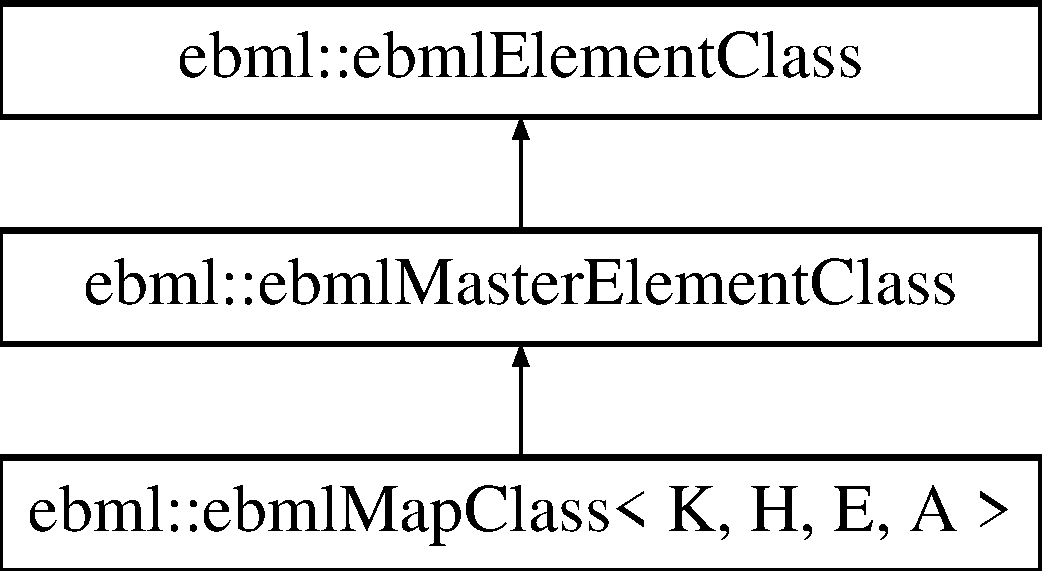
\includegraphics[height=3.000000cm]{classebml_1_1ebmlMapClass}
\end{center}
\end{figure}
\subsection*{Public Member Functions}
\begin{DoxyCompactItemize}
\item 
\mbox{\hyperlink{classebml_1_1ebmlMapClass_a54fe6d042e1b2e5c4ba9f8e3d7bba452}{ebml\+Map\+Class}} (const char $\ast$, const std\+::wstring \&, const \mbox{\hyperlink{classebml_1_1ebmlElementClass}{ebml\+Element\+Class}} $\ast$\mbox{\hyperlink{classebml_1_1ebmlMapClass_ad38f9bbe85f05f8865e9df739ab34792}{paircls}})
\item 
\mbox{\hyperlink{classebml_1_1ebmlMapClass_afe37bc0187986569ba263fe2a5e69915}{ebml\+Map\+Class}} (const char $\ast$, const std\+::wstring \&, const \mbox{\hyperlink{classebml_1_1ebmlPairClass}{ebml\+Pair\+Class}}$<$ const K $>$ $\ast$\mbox{\hyperlink{classebml_1_1ebmlMapClass_ad38f9bbe85f05f8865e9df739ab34792}{paircls}})
\item 
\mbox{\hyperlink{classebml_1_1ebmlMapClass_a27b494be5247aa4152bf994906ec117b}{ebml\+Map\+Class}} (\mbox{\hyperlink{namespaceebml_a86c5f604ddf12a74aa9812e997a58691}{ebml\+I\+D\+\_\+t}}, const std\+::wstring \&, const \mbox{\hyperlink{classebml_1_1ebmlElementClass}{ebml\+Element\+Class}} $\ast$\mbox{\hyperlink{classebml_1_1ebmlMapClass_ad38f9bbe85f05f8865e9df739ab34792}{paircls}})
\item 
\mbox{\hyperlink{classebml_1_1ebmlMapClass_a705b59b34949371aa925dc98e59213de}{ebml\+Map\+Class}} (\mbox{\hyperlink{namespaceebml_a86c5f604ddf12a74aa9812e997a58691}{ebml\+I\+D\+\_\+t}}, const std\+::wstring \&, const \mbox{\hyperlink{classebml_1_1ebmlPairClass}{ebml\+Pair\+Class}}$<$ const K $>$ $\ast$\mbox{\hyperlink{classebml_1_1ebmlMapClass_ad38f9bbe85f05f8865e9df739ab34792}{paircls}})
\item 
\mbox{\hyperlink{namespaceebml_adad533b7705a16bb360fe56380c5e7be}{ebml\+Element\+\_\+sp}} \mbox{\hyperlink{classebml_1_1ebmlMapClass_a92f0ffcbc555bdb6cbef10454a192640}{operator()}} () const
\item 
\mbox{\hyperlink{namespaceebml_adad533b7705a16bb360fe56380c5e7be}{ebml\+Element\+\_\+sp}} \mbox{\hyperlink{classebml_1_1ebmlMapClass_a65bc7cbdb0b605e7476222e28ebfcf46}{operator()}} (std\+::initializer\+\_\+list$<$ \mbox{\hyperlink{namespaceebml_adad533b7705a16bb360fe56380c5e7be}{ebml\+Element\+\_\+sp}} $>$) const
\item 
\mbox{\hyperlink{namespaceebml_adad533b7705a16bb360fe56380c5e7be}{ebml\+Element\+\_\+sp}} \mbox{\hyperlink{classebml_1_1ebmlMapClass_a8163549b01fe31fcb130f5bc8d4250d7}{operator()}} (std\+::initializer\+\_\+list$<$ std\+::pair$<$ \mbox{\hyperlink{namespaceebml_adad533b7705a16bb360fe56380c5e7be}{ebml\+Element\+\_\+sp}}, \mbox{\hyperlink{namespaceebml_adad533b7705a16bb360fe56380c5e7be}{ebml\+Element\+\_\+sp}} $>$$>$) const
\item 
\mbox{\hyperlink{namespaceebml_adad533b7705a16bb360fe56380c5e7be}{ebml\+Element\+\_\+sp}} \mbox{\hyperlink{classebml_1_1ebmlMapClass_adb3af4252af74bdd8ed824faad06ce55}{operator()}} (std\+::initializer\+\_\+list$<$ std\+::pair$<$ K, \mbox{\hyperlink{namespaceebml_adad533b7705a16bb360fe56380c5e7be}{ebml\+Element\+\_\+sp}} $>$$>$) const
\item 
\mbox{\hyperlink{namespaceebml_adad533b7705a16bb360fe56380c5e7be}{ebml\+Element\+\_\+sp}} \mbox{\hyperlink{classebml_1_1ebmlMapClass_a7dad33b823f99c48ea91bf28709edaf4}{operator()}} (const std\+::list$<$ \mbox{\hyperlink{namespaceebml_adad533b7705a16bb360fe56380c5e7be}{ebml\+Element\+\_\+sp}} $>$ \&) const
\item 
\mbox{\hyperlink{namespaceebml_adad533b7705a16bb360fe56380c5e7be}{ebml\+Element\+\_\+sp}} \mbox{\hyperlink{classebml_1_1ebmlMapClass_a4f498d6d1bff9b095c1a20243aff015f}{operator()}} (const std\+::list$<$ std\+::pair$<$ \mbox{\hyperlink{namespaceebml_adad533b7705a16bb360fe56380c5e7be}{ebml\+Element\+\_\+sp}}, \mbox{\hyperlink{namespaceebml_adad533b7705a16bb360fe56380c5e7be}{ebml\+Element\+\_\+sp}} $>$$>$ \&) const
\item 
\mbox{\hyperlink{namespaceebml_adad533b7705a16bb360fe56380c5e7be}{ebml\+Element\+\_\+sp}} \mbox{\hyperlink{classebml_1_1ebmlMapClass_ac1f975ed951299a2cc14e65b2d855bf9}{operator()}} (const std\+::list$<$ std\+::pair$<$ K, \mbox{\hyperlink{namespaceebml_adad533b7705a16bb360fe56380c5e7be}{ebml\+Element\+\_\+sp}} $>$$>$ \&) const
\item 
\mbox{\hyperlink{namespaceebml_adad533b7705a16bb360fe56380c5e7be}{ebml\+Element\+\_\+sp}} \mbox{\hyperlink{classebml_1_1ebmlMapClass_a4654bc73735e038eef9bca1c3f83ddc7}{operator()}} (std\+::list$<$ \mbox{\hyperlink{namespaceebml_adad533b7705a16bb360fe56380c5e7be}{ebml\+Element\+\_\+sp}} $>$ \&\&) const
\item 
\mbox{\hyperlink{namespaceebml_adad533b7705a16bb360fe56380c5e7be}{ebml\+Element\+\_\+sp}} \mbox{\hyperlink{classebml_1_1ebmlMapClass_a7a878bc5848a8f3886320b5043ec863a}{operator()}} (std\+::list$<$ std\+::pair$<$ \mbox{\hyperlink{namespaceebml_adad533b7705a16bb360fe56380c5e7be}{ebml\+Element\+\_\+sp}}, \mbox{\hyperlink{namespaceebml_adad533b7705a16bb360fe56380c5e7be}{ebml\+Element\+\_\+sp}} $>$$>$ \&\&) const
\item 
\mbox{\hyperlink{namespaceebml_adad533b7705a16bb360fe56380c5e7be}{ebml\+Element\+\_\+sp}} \mbox{\hyperlink{classebml_1_1ebmlMapClass_a7b3e1fcd73982391aa72cc0ece7d6fea}{operator()}} (std\+::list$<$ std\+::pair$<$ K, \mbox{\hyperlink{namespaceebml_adad533b7705a16bb360fe56380c5e7be}{ebml\+Element\+\_\+sp}} $>$$>$ \&\&) const
\item 
\mbox{\hyperlink{namespaceebml_adad533b7705a16bb360fe56380c5e7be}{ebml\+Element\+\_\+sp}} \mbox{\hyperlink{classebml_1_1ebmlMapClass_ad87e8698f2933cd7ee8980c68c0b6361}{operator()}} (const std\+::unordered\+\_\+map$<$ K, \mbox{\hyperlink{namespaceebml_adad533b7705a16bb360fe56380c5e7be}{ebml\+Element\+\_\+sp}}, H, E, A $>$ \&) const
\item 
\mbox{\hyperlink{namespaceebml_adad533b7705a16bb360fe56380c5e7be}{ebml\+Element\+\_\+sp}} \mbox{\hyperlink{classebml_1_1ebmlMapClass_a189fe07c7ef4e9cbe9b7bc39746a5a18}{operator()}} (std\+::unordered\+\_\+map$<$ K, \mbox{\hyperlink{namespaceebml_adad533b7705a16bb360fe56380c5e7be}{ebml\+Element\+\_\+sp}}, H, E, A $>$ \&\&) const
\item 
const \mbox{\hyperlink{classebml_1_1ebmlPairClass}{ebml\+Pair\+Class}}$<$ const K $>$ $\ast$ \mbox{\hyperlink{classebml_1_1ebmlMapClass_ad38f9bbe85f05f8865e9df739ab34792}{paircls}} () const
\end{DoxyCompactItemize}
\subsection*{Protected Member Functions}
\begin{DoxyCompactItemize}
\item 
\mbox{\hyperlink{classebml_1_1ebmlElement}{ebml\+Element}} $\ast$ \mbox{\hyperlink{classebml_1_1ebmlMapClass_a3370b9b3457982693c08723af7d5130a}{\+\_\+new}} () const
\end{DoxyCompactItemize}
\subsection*{Friends}
\begin{DoxyCompactItemize}
\item 
class \mbox{\hyperlink{classebml_1_1ebmlMapClass_a691e480013452ea48661a61746fd1b5c}{ebml\+Map$<$ K, H, E, A $>$}}
\end{DoxyCompactItemize}
\subsection*{Additional Inherited Members}


\subsection{Constructor \& Destructor Documentation}
\mbox{\Hypertarget{classebml_1_1ebmlMapClass_a54fe6d042e1b2e5c4ba9f8e3d7bba452}\label{classebml_1_1ebmlMapClass_a54fe6d042e1b2e5c4ba9f8e3d7bba452}} 
\index{ebml\+::ebml\+Map\+Class@{ebml\+::ebml\+Map\+Class}!ebml\+Map\+Class@{ebml\+Map\+Class}}
\index{ebml\+Map\+Class@{ebml\+Map\+Class}!ebml\+::ebml\+Map\+Class@{ebml\+::ebml\+Map\+Class}}
\subsubsection{\texorpdfstring{ebml\+Map\+Class()}{ebmlMapClass()}\hspace{0.1cm}{\footnotesize\ttfamily [1/4]}}
{\footnotesize\ttfamily template$<$typename K, typename H = std\+::hash$<$\+K$>$, typename E = std\+::equal\+\_\+to$<$\+K$>$, typename A = std\+::allocator$<$std\+::pair$<$const K, ebml\+Element\+\_\+sp$>$$>$$>$ \\
\mbox{\hyperlink{classebml_1_1ebmlMapClass}{ebml\+::ebml\+Map\+Class}}$<$ K, H, E, A $>$\+::\mbox{\hyperlink{classebml_1_1ebmlMapClass}{ebml\+Map\+Class}} (\begin{DoxyParamCaption}\item[{const char $\ast$}]{,  }\item[{const std\+::wstring \&}]{,  }\item[{const \mbox{\hyperlink{classebml_1_1ebmlElementClass}{ebml\+Element\+Class}} $\ast$}]{paircls }\end{DoxyParamCaption})}

\mbox{\Hypertarget{classebml_1_1ebmlMapClass_afe37bc0187986569ba263fe2a5e69915}\label{classebml_1_1ebmlMapClass_afe37bc0187986569ba263fe2a5e69915}} 
\index{ebml\+::ebml\+Map\+Class@{ebml\+::ebml\+Map\+Class}!ebml\+Map\+Class@{ebml\+Map\+Class}}
\index{ebml\+Map\+Class@{ebml\+Map\+Class}!ebml\+::ebml\+Map\+Class@{ebml\+::ebml\+Map\+Class}}
\subsubsection{\texorpdfstring{ebml\+Map\+Class()}{ebmlMapClass()}\hspace{0.1cm}{\footnotesize\ttfamily [2/4]}}
{\footnotesize\ttfamily template$<$typename K, typename H = std\+::hash$<$\+K$>$, typename E = std\+::equal\+\_\+to$<$\+K$>$, typename A = std\+::allocator$<$std\+::pair$<$const K, ebml\+Element\+\_\+sp$>$$>$$>$ \\
\mbox{\hyperlink{classebml_1_1ebmlMapClass}{ebml\+::ebml\+Map\+Class}}$<$ K, H, E, A $>$\+::\mbox{\hyperlink{classebml_1_1ebmlMapClass}{ebml\+Map\+Class}} (\begin{DoxyParamCaption}\item[{const char $\ast$}]{,  }\item[{const std\+::wstring \&}]{,  }\item[{const \mbox{\hyperlink{classebml_1_1ebmlPairClass}{ebml\+Pair\+Class}}$<$ const K $>$ $\ast$}]{paircls }\end{DoxyParamCaption})}

\mbox{\Hypertarget{classebml_1_1ebmlMapClass_a27b494be5247aa4152bf994906ec117b}\label{classebml_1_1ebmlMapClass_a27b494be5247aa4152bf994906ec117b}} 
\index{ebml\+::ebml\+Map\+Class@{ebml\+::ebml\+Map\+Class}!ebml\+Map\+Class@{ebml\+Map\+Class}}
\index{ebml\+Map\+Class@{ebml\+Map\+Class}!ebml\+::ebml\+Map\+Class@{ebml\+::ebml\+Map\+Class}}
\subsubsection{\texorpdfstring{ebml\+Map\+Class()}{ebmlMapClass()}\hspace{0.1cm}{\footnotesize\ttfamily [3/4]}}
{\footnotesize\ttfamily template$<$typename K, typename H = std\+::hash$<$\+K$>$, typename E = std\+::equal\+\_\+to$<$\+K$>$, typename A = std\+::allocator$<$std\+::pair$<$const K, ebml\+Element\+\_\+sp$>$$>$$>$ \\
\mbox{\hyperlink{classebml_1_1ebmlMapClass}{ebml\+::ebml\+Map\+Class}}$<$ K, H, E, A $>$\+::\mbox{\hyperlink{classebml_1_1ebmlMapClass}{ebml\+Map\+Class}} (\begin{DoxyParamCaption}\item[{\mbox{\hyperlink{namespaceebml_a86c5f604ddf12a74aa9812e997a58691}{ebml\+I\+D\+\_\+t}}}]{,  }\item[{const std\+::wstring \&}]{,  }\item[{const \mbox{\hyperlink{classebml_1_1ebmlElementClass}{ebml\+Element\+Class}} $\ast$}]{paircls }\end{DoxyParamCaption})}

\mbox{\Hypertarget{classebml_1_1ebmlMapClass_a705b59b34949371aa925dc98e59213de}\label{classebml_1_1ebmlMapClass_a705b59b34949371aa925dc98e59213de}} 
\index{ebml\+::ebml\+Map\+Class@{ebml\+::ebml\+Map\+Class}!ebml\+Map\+Class@{ebml\+Map\+Class}}
\index{ebml\+Map\+Class@{ebml\+Map\+Class}!ebml\+::ebml\+Map\+Class@{ebml\+::ebml\+Map\+Class}}
\subsubsection{\texorpdfstring{ebml\+Map\+Class()}{ebmlMapClass()}\hspace{0.1cm}{\footnotesize\ttfamily [4/4]}}
{\footnotesize\ttfamily template$<$typename K, typename H = std\+::hash$<$\+K$>$, typename E = std\+::equal\+\_\+to$<$\+K$>$, typename A = std\+::allocator$<$std\+::pair$<$const K, ebml\+Element\+\_\+sp$>$$>$$>$ \\
\mbox{\hyperlink{classebml_1_1ebmlMapClass}{ebml\+::ebml\+Map\+Class}}$<$ K, H, E, A $>$\+::\mbox{\hyperlink{classebml_1_1ebmlMapClass}{ebml\+Map\+Class}} (\begin{DoxyParamCaption}\item[{\mbox{\hyperlink{namespaceebml_a86c5f604ddf12a74aa9812e997a58691}{ebml\+I\+D\+\_\+t}}}]{,  }\item[{const std\+::wstring \&}]{,  }\item[{const \mbox{\hyperlink{classebml_1_1ebmlPairClass}{ebml\+Pair\+Class}}$<$ const K $>$ $\ast$}]{paircls }\end{DoxyParamCaption})}



\subsection{Member Function Documentation}
\mbox{\Hypertarget{classebml_1_1ebmlMapClass_a3370b9b3457982693c08723af7d5130a}\label{classebml_1_1ebmlMapClass_a3370b9b3457982693c08723af7d5130a}} 
\index{ebml\+::ebml\+Map\+Class@{ebml\+::ebml\+Map\+Class}!\+\_\+new@{\+\_\+new}}
\index{\+\_\+new@{\+\_\+new}!ebml\+::ebml\+Map\+Class@{ebml\+::ebml\+Map\+Class}}
\subsubsection{\texorpdfstring{\+\_\+new()}{\_new()}}
{\footnotesize\ttfamily template$<$typename K, typename H = std\+::hash$<$\+K$>$, typename E = std\+::equal\+\_\+to$<$\+K$>$, typename A = std\+::allocator$<$std\+::pair$<$const K, ebml\+Element\+\_\+sp$>$$>$$>$ \\
\mbox{\hyperlink{classebml_1_1ebmlElement}{ebml\+Element}}$\ast$ \mbox{\hyperlink{classebml_1_1ebmlMapClass}{ebml\+::ebml\+Map\+Class}}$<$ K, H, E, A $>$\+::\+\_\+new (\begin{DoxyParamCaption}{ }\end{DoxyParamCaption}) const\hspace{0.3cm}{\ttfamily [protected]}, {\ttfamily [virtual]}}



Implements \mbox{\hyperlink{classebml_1_1ebmlElementClass_a223ede6b8bc3c85251d2d73f0256fb45}{ebml\+::ebml\+Element\+Class}}.

\mbox{\Hypertarget{classebml_1_1ebmlMapClass_a92f0ffcbc555bdb6cbef10454a192640}\label{classebml_1_1ebmlMapClass_a92f0ffcbc555bdb6cbef10454a192640}} 
\index{ebml\+::ebml\+Map\+Class@{ebml\+::ebml\+Map\+Class}!operator()@{operator()}}
\index{operator()@{operator()}!ebml\+::ebml\+Map\+Class@{ebml\+::ebml\+Map\+Class}}
\subsubsection{\texorpdfstring{operator()()}{operator()()}\hspace{0.1cm}{\footnotesize\ttfamily [1/12]}}
{\footnotesize\ttfamily template$<$typename K, typename H = std\+::hash$<$\+K$>$, typename E = std\+::equal\+\_\+to$<$\+K$>$, typename A = std\+::allocator$<$std\+::pair$<$const K, ebml\+Element\+\_\+sp$>$$>$$>$ \\
\mbox{\hyperlink{namespaceebml_adad533b7705a16bb360fe56380c5e7be}{ebml\+Element\+\_\+sp}} \mbox{\hyperlink{classebml_1_1ebmlMapClass}{ebml\+::ebml\+Map\+Class}}$<$ K, H, E, A $>$\+::operator() (\begin{DoxyParamCaption}{ }\end{DoxyParamCaption}) const}

\mbox{\Hypertarget{classebml_1_1ebmlMapClass_a65bc7cbdb0b605e7476222e28ebfcf46}\label{classebml_1_1ebmlMapClass_a65bc7cbdb0b605e7476222e28ebfcf46}} 
\index{ebml\+::ebml\+Map\+Class@{ebml\+::ebml\+Map\+Class}!operator()@{operator()}}
\index{operator()@{operator()}!ebml\+::ebml\+Map\+Class@{ebml\+::ebml\+Map\+Class}}
\subsubsection{\texorpdfstring{operator()()}{operator()()}\hspace{0.1cm}{\footnotesize\ttfamily [2/12]}}
{\footnotesize\ttfamily template$<$typename K, typename H = std\+::hash$<$\+K$>$, typename E = std\+::equal\+\_\+to$<$\+K$>$, typename A = std\+::allocator$<$std\+::pair$<$const K, ebml\+Element\+\_\+sp$>$$>$$>$ \\
\mbox{\hyperlink{namespaceebml_adad533b7705a16bb360fe56380c5e7be}{ebml\+Element\+\_\+sp}} \mbox{\hyperlink{classebml_1_1ebmlMapClass}{ebml\+::ebml\+Map\+Class}}$<$ K, H, E, A $>$\+::operator() (\begin{DoxyParamCaption}\item[{std\+::initializer\+\_\+list$<$ \mbox{\hyperlink{namespaceebml_adad533b7705a16bb360fe56380c5e7be}{ebml\+Element\+\_\+sp}} $>$}]{ }\end{DoxyParamCaption}) const}

\mbox{\Hypertarget{classebml_1_1ebmlMapClass_a8163549b01fe31fcb130f5bc8d4250d7}\label{classebml_1_1ebmlMapClass_a8163549b01fe31fcb130f5bc8d4250d7}} 
\index{ebml\+::ebml\+Map\+Class@{ebml\+::ebml\+Map\+Class}!operator()@{operator()}}
\index{operator()@{operator()}!ebml\+::ebml\+Map\+Class@{ebml\+::ebml\+Map\+Class}}
\subsubsection{\texorpdfstring{operator()()}{operator()()}\hspace{0.1cm}{\footnotesize\ttfamily [3/12]}}
{\footnotesize\ttfamily template$<$typename K, typename H = std\+::hash$<$\+K$>$, typename E = std\+::equal\+\_\+to$<$\+K$>$, typename A = std\+::allocator$<$std\+::pair$<$const K, ebml\+Element\+\_\+sp$>$$>$$>$ \\
\mbox{\hyperlink{namespaceebml_adad533b7705a16bb360fe56380c5e7be}{ebml\+Element\+\_\+sp}} \mbox{\hyperlink{classebml_1_1ebmlMapClass}{ebml\+::ebml\+Map\+Class}}$<$ K, H, E, A $>$\+::operator() (\begin{DoxyParamCaption}{ }\end{DoxyParamCaption})}

\mbox{\Hypertarget{classebml_1_1ebmlMapClass_adb3af4252af74bdd8ed824faad06ce55}\label{classebml_1_1ebmlMapClass_adb3af4252af74bdd8ed824faad06ce55}} 
\index{ebml\+::ebml\+Map\+Class@{ebml\+::ebml\+Map\+Class}!operator()@{operator()}}
\index{operator()@{operator()}!ebml\+::ebml\+Map\+Class@{ebml\+::ebml\+Map\+Class}}
\subsubsection{\texorpdfstring{operator()()}{operator()()}\hspace{0.1cm}{\footnotesize\ttfamily [4/12]}}
{\footnotesize\ttfamily template$<$typename K, typename H = std\+::hash$<$\+K$>$, typename E = std\+::equal\+\_\+to$<$\+K$>$, typename A = std\+::allocator$<$std\+::pair$<$const K, ebml\+Element\+\_\+sp$>$$>$$>$ \\
\mbox{\hyperlink{namespaceebml_adad533b7705a16bb360fe56380c5e7be}{ebml\+Element\+\_\+sp}} \mbox{\hyperlink{classebml_1_1ebmlMapClass}{ebml\+::ebml\+Map\+Class}}$<$ K, H, E, A $>$\+::operator() (\begin{DoxyParamCaption}{ }\end{DoxyParamCaption})}

\mbox{\Hypertarget{classebml_1_1ebmlMapClass_a7dad33b823f99c48ea91bf28709edaf4}\label{classebml_1_1ebmlMapClass_a7dad33b823f99c48ea91bf28709edaf4}} 
\index{ebml\+::ebml\+Map\+Class@{ebml\+::ebml\+Map\+Class}!operator()@{operator()}}
\index{operator()@{operator()}!ebml\+::ebml\+Map\+Class@{ebml\+::ebml\+Map\+Class}}
\subsubsection{\texorpdfstring{operator()()}{operator()()}\hspace{0.1cm}{\footnotesize\ttfamily [5/12]}}
{\footnotesize\ttfamily template$<$typename K, typename H = std\+::hash$<$\+K$>$, typename E = std\+::equal\+\_\+to$<$\+K$>$, typename A = std\+::allocator$<$std\+::pair$<$const K, ebml\+Element\+\_\+sp$>$$>$$>$ \\
\mbox{\hyperlink{namespaceebml_adad533b7705a16bb360fe56380c5e7be}{ebml\+Element\+\_\+sp}} \mbox{\hyperlink{classebml_1_1ebmlMapClass}{ebml\+::ebml\+Map\+Class}}$<$ K, H, E, A $>$\+::operator() (\begin{DoxyParamCaption}\item[{const std\+::list$<$ \mbox{\hyperlink{namespaceebml_adad533b7705a16bb360fe56380c5e7be}{ebml\+Element\+\_\+sp}} $>$ \&}]{ }\end{DoxyParamCaption}) const}

\mbox{\Hypertarget{classebml_1_1ebmlMapClass_a4f498d6d1bff9b095c1a20243aff015f}\label{classebml_1_1ebmlMapClass_a4f498d6d1bff9b095c1a20243aff015f}} 
\index{ebml\+::ebml\+Map\+Class@{ebml\+::ebml\+Map\+Class}!operator()@{operator()}}
\index{operator()@{operator()}!ebml\+::ebml\+Map\+Class@{ebml\+::ebml\+Map\+Class}}
\subsubsection{\texorpdfstring{operator()()}{operator()()}\hspace{0.1cm}{\footnotesize\ttfamily [6/12]}}
{\footnotesize\ttfamily template$<$typename K, typename H = std\+::hash$<$\+K$>$, typename E = std\+::equal\+\_\+to$<$\+K$>$, typename A = std\+::allocator$<$std\+::pair$<$const K, ebml\+Element\+\_\+sp$>$$>$$>$ \\
\mbox{\hyperlink{namespaceebml_adad533b7705a16bb360fe56380c5e7be}{ebml\+Element\+\_\+sp}} \mbox{\hyperlink{classebml_1_1ebmlMapClass}{ebml\+::ebml\+Map\+Class}}$<$ K, H, E, A $>$\+::operator() (\begin{DoxyParamCaption}\item[{const std\+::list$<$ std\+::pair$<$ \mbox{\hyperlink{namespaceebml_adad533b7705a16bb360fe56380c5e7be}{ebml\+Element\+\_\+sp}}, \mbox{\hyperlink{namespaceebml_adad533b7705a16bb360fe56380c5e7be}{ebml\+Element\+\_\+sp}} $>$$>$ \&}]{ }\end{DoxyParamCaption}) const}

\mbox{\Hypertarget{classebml_1_1ebmlMapClass_ac1f975ed951299a2cc14e65b2d855bf9}\label{classebml_1_1ebmlMapClass_ac1f975ed951299a2cc14e65b2d855bf9}} 
\index{ebml\+::ebml\+Map\+Class@{ebml\+::ebml\+Map\+Class}!operator()@{operator()}}
\index{operator()@{operator()}!ebml\+::ebml\+Map\+Class@{ebml\+::ebml\+Map\+Class}}
\subsubsection{\texorpdfstring{operator()()}{operator()()}\hspace{0.1cm}{\footnotesize\ttfamily [7/12]}}
{\footnotesize\ttfamily template$<$typename K, typename H = std\+::hash$<$\+K$>$, typename E = std\+::equal\+\_\+to$<$\+K$>$, typename A = std\+::allocator$<$std\+::pair$<$const K, ebml\+Element\+\_\+sp$>$$>$$>$ \\
\mbox{\hyperlink{namespaceebml_adad533b7705a16bb360fe56380c5e7be}{ebml\+Element\+\_\+sp}} \mbox{\hyperlink{classebml_1_1ebmlMapClass}{ebml\+::ebml\+Map\+Class}}$<$ K, H, E, A $>$\+::operator() (\begin{DoxyParamCaption}\item[{const std\+::list$<$ std\+::pair$<$ K, \mbox{\hyperlink{namespaceebml_adad533b7705a16bb360fe56380c5e7be}{ebml\+Element\+\_\+sp}} $>$$>$ \&}]{ }\end{DoxyParamCaption}) const}

\mbox{\Hypertarget{classebml_1_1ebmlMapClass_a4654bc73735e038eef9bca1c3f83ddc7}\label{classebml_1_1ebmlMapClass_a4654bc73735e038eef9bca1c3f83ddc7}} 
\index{ebml\+::ebml\+Map\+Class@{ebml\+::ebml\+Map\+Class}!operator()@{operator()}}
\index{operator()@{operator()}!ebml\+::ebml\+Map\+Class@{ebml\+::ebml\+Map\+Class}}
\subsubsection{\texorpdfstring{operator()()}{operator()()}\hspace{0.1cm}{\footnotesize\ttfamily [8/12]}}
{\footnotesize\ttfamily template$<$typename K, typename H = std\+::hash$<$\+K$>$, typename E = std\+::equal\+\_\+to$<$\+K$>$, typename A = std\+::allocator$<$std\+::pair$<$const K, ebml\+Element\+\_\+sp$>$$>$$>$ \\
\mbox{\hyperlink{namespaceebml_adad533b7705a16bb360fe56380c5e7be}{ebml\+Element\+\_\+sp}} \mbox{\hyperlink{classebml_1_1ebmlMapClass}{ebml\+::ebml\+Map\+Class}}$<$ K, H, E, A $>$\+::operator() (\begin{DoxyParamCaption}\item[{std\+::list$<$ \mbox{\hyperlink{namespaceebml_adad533b7705a16bb360fe56380c5e7be}{ebml\+Element\+\_\+sp}} $>$ \&\&}]{ }\end{DoxyParamCaption}) const}

\mbox{\Hypertarget{classebml_1_1ebmlMapClass_a7a878bc5848a8f3886320b5043ec863a}\label{classebml_1_1ebmlMapClass_a7a878bc5848a8f3886320b5043ec863a}} 
\index{ebml\+::ebml\+Map\+Class@{ebml\+::ebml\+Map\+Class}!operator()@{operator()}}
\index{operator()@{operator()}!ebml\+::ebml\+Map\+Class@{ebml\+::ebml\+Map\+Class}}
\subsubsection{\texorpdfstring{operator()()}{operator()()}\hspace{0.1cm}{\footnotesize\ttfamily [9/12]}}
{\footnotesize\ttfamily template$<$typename K, typename H = std\+::hash$<$\+K$>$, typename E = std\+::equal\+\_\+to$<$\+K$>$, typename A = std\+::allocator$<$std\+::pair$<$const K, ebml\+Element\+\_\+sp$>$$>$$>$ \\
\mbox{\hyperlink{namespaceebml_adad533b7705a16bb360fe56380c5e7be}{ebml\+Element\+\_\+sp}} \mbox{\hyperlink{classebml_1_1ebmlMapClass}{ebml\+::ebml\+Map\+Class}}$<$ K, H, E, A $>$\+::operator() (\begin{DoxyParamCaption}\item[{std\+::list$<$ std\+::pair$<$ \mbox{\hyperlink{namespaceebml_adad533b7705a16bb360fe56380c5e7be}{ebml\+Element\+\_\+sp}}, \mbox{\hyperlink{namespaceebml_adad533b7705a16bb360fe56380c5e7be}{ebml\+Element\+\_\+sp}} $>$$>$ \&\&}]{ }\end{DoxyParamCaption}) const}

\mbox{\Hypertarget{classebml_1_1ebmlMapClass_a7b3e1fcd73982391aa72cc0ece7d6fea}\label{classebml_1_1ebmlMapClass_a7b3e1fcd73982391aa72cc0ece7d6fea}} 
\index{ebml\+::ebml\+Map\+Class@{ebml\+::ebml\+Map\+Class}!operator()@{operator()}}
\index{operator()@{operator()}!ebml\+::ebml\+Map\+Class@{ebml\+::ebml\+Map\+Class}}
\subsubsection{\texorpdfstring{operator()()}{operator()()}\hspace{0.1cm}{\footnotesize\ttfamily [10/12]}}
{\footnotesize\ttfamily template$<$typename K, typename H = std\+::hash$<$\+K$>$, typename E = std\+::equal\+\_\+to$<$\+K$>$, typename A = std\+::allocator$<$std\+::pair$<$const K, ebml\+Element\+\_\+sp$>$$>$$>$ \\
\mbox{\hyperlink{namespaceebml_adad533b7705a16bb360fe56380c5e7be}{ebml\+Element\+\_\+sp}} \mbox{\hyperlink{classebml_1_1ebmlMapClass}{ebml\+::ebml\+Map\+Class}}$<$ K, H, E, A $>$\+::operator() (\begin{DoxyParamCaption}\item[{std\+::list$<$ std\+::pair$<$ K, \mbox{\hyperlink{namespaceebml_adad533b7705a16bb360fe56380c5e7be}{ebml\+Element\+\_\+sp}} $>$$>$ \&\&}]{ }\end{DoxyParamCaption}) const}

\mbox{\Hypertarget{classebml_1_1ebmlMapClass_ad87e8698f2933cd7ee8980c68c0b6361}\label{classebml_1_1ebmlMapClass_ad87e8698f2933cd7ee8980c68c0b6361}} 
\index{ebml\+::ebml\+Map\+Class@{ebml\+::ebml\+Map\+Class}!operator()@{operator()}}
\index{operator()@{operator()}!ebml\+::ebml\+Map\+Class@{ebml\+::ebml\+Map\+Class}}
\subsubsection{\texorpdfstring{operator()()}{operator()()}\hspace{0.1cm}{\footnotesize\ttfamily [11/12]}}
{\footnotesize\ttfamily template$<$typename K, typename H = std\+::hash$<$\+K$>$, typename E = std\+::equal\+\_\+to$<$\+K$>$, typename A = std\+::allocator$<$std\+::pair$<$const K, ebml\+Element\+\_\+sp$>$$>$$>$ \\
\mbox{\hyperlink{namespaceebml_adad533b7705a16bb360fe56380c5e7be}{ebml\+Element\+\_\+sp}} \mbox{\hyperlink{classebml_1_1ebmlMapClass}{ebml\+::ebml\+Map\+Class}}$<$ K, H, E, A $>$\+::operator() (\begin{DoxyParamCaption}\item[{const std\+::unordered\+\_\+map$<$ K, \mbox{\hyperlink{namespaceebml_adad533b7705a16bb360fe56380c5e7be}{ebml\+Element\+\_\+sp}}, H, E, A $>$ \&}]{ }\end{DoxyParamCaption}) const}

\mbox{\Hypertarget{classebml_1_1ebmlMapClass_a189fe07c7ef4e9cbe9b7bc39746a5a18}\label{classebml_1_1ebmlMapClass_a189fe07c7ef4e9cbe9b7bc39746a5a18}} 
\index{ebml\+::ebml\+Map\+Class@{ebml\+::ebml\+Map\+Class}!operator()@{operator()}}
\index{operator()@{operator()}!ebml\+::ebml\+Map\+Class@{ebml\+::ebml\+Map\+Class}}
\subsubsection{\texorpdfstring{operator()()}{operator()()}\hspace{0.1cm}{\footnotesize\ttfamily [12/12]}}
{\footnotesize\ttfamily template$<$typename K, typename H = std\+::hash$<$\+K$>$, typename E = std\+::equal\+\_\+to$<$\+K$>$, typename A = std\+::allocator$<$std\+::pair$<$const K, ebml\+Element\+\_\+sp$>$$>$$>$ \\
\mbox{\hyperlink{namespaceebml_adad533b7705a16bb360fe56380c5e7be}{ebml\+Element\+\_\+sp}} \mbox{\hyperlink{classebml_1_1ebmlMapClass}{ebml\+::ebml\+Map\+Class}}$<$ K, H, E, A $>$\+::operator() (\begin{DoxyParamCaption}\item[{std\+::unordered\+\_\+map$<$ K, \mbox{\hyperlink{namespaceebml_adad533b7705a16bb360fe56380c5e7be}{ebml\+Element\+\_\+sp}}, H, E, A $>$ \&\&}]{ }\end{DoxyParamCaption}) const}

\mbox{\Hypertarget{classebml_1_1ebmlMapClass_ad38f9bbe85f05f8865e9df739ab34792}\label{classebml_1_1ebmlMapClass_ad38f9bbe85f05f8865e9df739ab34792}} 
\index{ebml\+::ebml\+Map\+Class@{ebml\+::ebml\+Map\+Class}!paircls@{paircls}}
\index{paircls@{paircls}!ebml\+::ebml\+Map\+Class@{ebml\+::ebml\+Map\+Class}}
\subsubsection{\texorpdfstring{paircls()}{paircls()}}
{\footnotesize\ttfamily template$<$typename K, typename H = std\+::hash$<$\+K$>$, typename E = std\+::equal\+\_\+to$<$\+K$>$, typename A = std\+::allocator$<$std\+::pair$<$const K, ebml\+Element\+\_\+sp$>$$>$$>$ \\
const \mbox{\hyperlink{classebml_1_1ebmlPairClass}{ebml\+Pair\+Class}}$<$const K$>$$\ast$ \mbox{\hyperlink{classebml_1_1ebmlMapClass}{ebml\+::ebml\+Map\+Class}}$<$ K, H, E, A $>$\+::paircls (\begin{DoxyParamCaption}{ }\end{DoxyParamCaption}) const}



\subsection{Friends And Related Function Documentation}
\mbox{\Hypertarget{classebml_1_1ebmlMapClass_a691e480013452ea48661a61746fd1b5c}\label{classebml_1_1ebmlMapClass_a691e480013452ea48661a61746fd1b5c}} 
\index{ebml\+::ebml\+Map\+Class@{ebml\+::ebml\+Map\+Class}!ebml\+Map$<$ K, H, E, A $>$@{ebml\+Map$<$ K, H, E, A $>$}}
\index{ebml\+Map$<$ K, H, E, A $>$@{ebml\+Map$<$ K, H, E, A $>$}!ebml\+::ebml\+Map\+Class@{ebml\+::ebml\+Map\+Class}}
\subsubsection{\texorpdfstring{ebml\+Map$<$ K, H, E, A $>$}{ebmlMap< K, H, E, A >}}
{\footnotesize\ttfamily template$<$typename K, typename H = std\+::hash$<$\+K$>$, typename E = std\+::equal\+\_\+to$<$\+K$>$, typename A = std\+::allocator$<$std\+::pair$<$const K, ebml\+Element\+\_\+sp$>$$>$$>$ \\
friend class \mbox{\hyperlink{classebml_1_1ebmlMap}{ebml\+Map}}$<$ K, H, E, A $>$\hspace{0.3cm}{\ttfamily [friend]}}



The documentation for this class was generated from the following file\+:\begin{DoxyCompactItemize}
\item 
include/libebml\+\_\+ng/masterelement/\mbox{\hyperlink{map_8h}{map.\+h}}\end{DoxyCompactItemize}

\hypertarget{classebml_1_1ebmlMasterElement}{}\section{ebml\+:\+:ebml\+Master\+Element Class Reference}
\label{classebml_1_1ebmlMasterElement}\index{ebml\+::ebml\+Master\+Element@{ebml\+::ebml\+Master\+Element}}


{\ttfamily \#include $<$base.\+h$>$}

Inheritance diagram for ebml\+:\+:ebml\+Master\+Element\+:\begin{figure}[H]
\begin{center}
\leavevmode
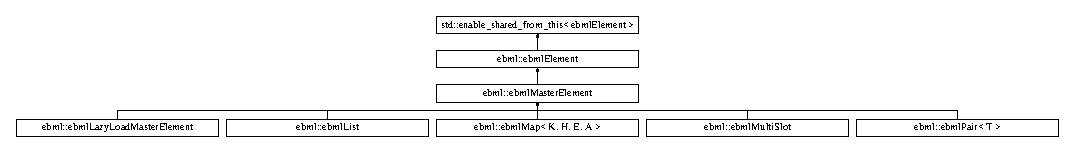
\includegraphics[height=1.611511cm]{classebml_1_1ebmlMasterElement}
\end{center}
\end{figure}
\subsection*{Classes}
\begin{DoxyCompactItemize}
\item 
class \mbox{\hyperlink{classebml_1_1ebmlMasterElement_1_1__const__iterator}{\+\_\+const\+\_\+iterator}}
\item 
class \mbox{\hyperlink{classebml_1_1ebmlMasterElement_1_1__iterator}{\+\_\+iterator}}
\item 
class \mbox{\hyperlink{classebml_1_1ebmlMasterElement_1_1const__iterator}{const\+\_\+iterator}}
\item 
class \mbox{\hyperlink{classebml_1_1ebmlMasterElement_1_1iterator}{iterator}}
\end{DoxyCompactItemize}
\subsection*{Public Member Functions}
\begin{DoxyCompactItemize}
\item 
size\+\_\+t \mbox{\hyperlink{classebml_1_1ebmlMasterElement_ae396f9a2f9e0e86b7f6d20505b88352c}{data\+Size}} () const
\item 
\mbox{\hyperlink{structebml_1_1sizetree__t}{sizetree\+\_\+t}} \mbox{\hyperlink{classebml_1_1ebmlMasterElement_a144f54d1231432975a47f4f83fd2e068}{sizetree}} () const
\item 
std\+::string \mbox{\hyperlink{classebml_1_1ebmlMasterElement_a2016b30a9ac7d48e990a6a864138a362}{encode}} () const
\item 
size\+\_\+t \mbox{\hyperlink{classebml_1_1ebmlMasterElement_ac0bc9d595746939fea3e30b810d89c9f}{encode}} (char $\ast$) const
\item 
size\+\_\+t \mbox{\hyperlink{classebml_1_1ebmlMasterElement_af9c776725a15ddff8a66d6c42bb7610f}{encode}} (char $\ast$, const \mbox{\hyperlink{structebml_1_1sizetree__t}{sizetree\+\_\+t}} \&) const
\item 
\mbox{\hyperlink{classebml_1_1ebmlMasterElement_1_1iterator}{iterator}} \mbox{\hyperlink{classebml_1_1ebmlMasterElement_aee8637a10705708acad5add971ac6999}{begin}} ()
\item 
\mbox{\hyperlink{classebml_1_1ebmlMasterElement_1_1iterator}{iterator}} \mbox{\hyperlink{classebml_1_1ebmlMasterElement_a9859bf4ba74c58ccc0eef1c9f6017719}{end}} ()
\item 
\mbox{\hyperlink{classebml_1_1ebmlMasterElement_1_1const__iterator}{const\+\_\+iterator}} \mbox{\hyperlink{classebml_1_1ebmlMasterElement_af8869286e051067d82fad936eb0c7a74}{cbegin}} () const
\item 
\mbox{\hyperlink{classebml_1_1ebmlMasterElement_1_1const__iterator}{const\+\_\+iterator}} \mbox{\hyperlink{classebml_1_1ebmlMasterElement_a7e4fa27c47c71e99615452dc4e1e3190}{cend}} () const
\end{DoxyCompactItemize}
\subsection*{Protected Member Functions}
\begin{DoxyCompactItemize}
\item 
\mbox{\hyperlink{classebml_1_1ebmlMasterElement_a874430a761ddf6eeb704d40136e75d33}{ebml\+Master\+Element}} (const \mbox{\hyperlink{classebml_1_1ebmlMasterElementClass}{ebml\+Master\+Element\+Class}} $\ast$)
\item 
virtual const \mbox{\hyperlink{classebml_1_1ebmlMasterElementClass}{ebml\+Master\+Element\+Class}} $\ast$ \mbox{\hyperlink{classebml_1_1ebmlMasterElement_a4073fb3f7ce3dda153384821714df29e}{cls}} () const
\item 
size\+\_\+t \mbox{\hyperlink{classebml_1_1ebmlMasterElement_ab50b9cdd8e402150cd96a19d613c98f5}{\+\_\+encode}} (char $\ast$, const \mbox{\hyperlink{structebml_1_1sizetree__t}{sizetree\+\_\+t}} \&) const
\item 
size\+\_\+t \mbox{\hyperlink{classebml_1_1ebmlMasterElement_aa0dd7215a5de90f8a52364df781952e2}{\+\_\+encode}} (char $\ast$) const
\item 
virtual void \mbox{\hyperlink{classebml_1_1ebmlMasterElement_a2fdf9fa1022f06a046fe94e631e266a3}{\+\_\+clear}} ()
\item 
virtual void \mbox{\hyperlink{classebml_1_1ebmlMasterElement_ae486adb2522e8d10177c70d889c32922}{\+\_\+decode\+Children}} (\mbox{\hyperlink{classebml_1_1parseString_1_1iterator}{parse\+String\+::iterator}} \&)
\item 
virtual void \mbox{\hyperlink{classebml_1_1ebmlMasterElement_af4b802cb2b71b57215d6e0f25f9fa25e}{\+\_\+cdecode\+Children}} (\mbox{\hyperlink{classebml_1_1parseString_1_1iterator}{parse\+String\+::iterator}} \&)
\item 
virtual void \mbox{\hyperlink{classebml_1_1ebmlMasterElement_a233be2f503f44d36608b16db5a2c3394}{\+\_\+scan\+Children}} (\mbox{\hyperlink{classebml_1_1parseFile_1_1iterator}{parse\+File\+::iterator}} \&)
\item 
virtual void \mbox{\hyperlink{classebml_1_1ebmlMasterElement_ab0cf3b000a54169e233f38aef9dcb4e1}{\+\_\+handle\+Parse\+File}} (const \mbox{\hyperlink{classebml_1_1parseFile}{parse\+File}} \&)
\item 
virtual void \mbox{\hyperlink{classebml_1_1ebmlMasterElement_a5c076b30207aefe6f6ecc46de3b96379}{\+\_\+cscan\+Children}} (\mbox{\hyperlink{classebml_1_1parseFile_1_1iterator}{parse\+File\+::iterator}} \&)
\item 
virtual void \mbox{\hyperlink{classebml_1_1ebmlMasterElement_a1d1d86beffcd09cbf1ede321c088ef17}{\+\_\+chandle\+Parse\+File}} (const \mbox{\hyperlink{classebml_1_1parseFile}{parse\+File}} \&)
\item 
virtual void \mbox{\hyperlink{classebml_1_1ebmlMasterElement_a59c5f3b3409fd5fd6f0f22c7a68f1c9b}{\+\_\+add\+Child}} (const \mbox{\hyperlink{namespaceebml_adad533b7705a16bb360fe56380c5e7be}{ebml\+Element\+\_\+sp}} \&)=0
\item 
virtual void \mbox{\hyperlink{classebml_1_1ebmlMasterElement_a3af0270846a1ced1719d26dd261f0355}{\+\_\+add\+Child}} (\mbox{\hyperlink{namespaceebml_adad533b7705a16bb360fe56380c5e7be}{ebml\+Element\+\_\+sp}} \&\&)=0
\item 
virtual \mbox{\hyperlink{classebml_1_1ebmlMasterElement_1_1__iterator}{ebml\+Master\+Element\+::\+\_\+iterator}} $\ast$ \mbox{\hyperlink{classebml_1_1ebmlMasterElement_af6fb7a9934e9b8d0c64273ef6944f44b}{\+\_\+begin}} ()=0
\item 
virtual \mbox{\hyperlink{classebml_1_1ebmlMasterElement_1_1__iterator}{ebml\+Master\+Element\+::\+\_\+iterator}} $\ast$ \mbox{\hyperlink{classebml_1_1ebmlMasterElement_a352e5e11836063394990cb05c09d8e48}{\+\_\+end}} ()=0
\item 
virtual \mbox{\hyperlink{classebml_1_1ebmlMasterElement_1_1__const__iterator}{ebml\+Master\+Element\+::\+\_\+const\+\_\+iterator}} $\ast$ \mbox{\hyperlink{classebml_1_1ebmlMasterElement_a7e1ffa498e22b637a6671df14aa0bc45}{\+\_\+cbegin}} () const =0
\item 
virtual \mbox{\hyperlink{classebml_1_1ebmlMasterElement_1_1__const__iterator}{ebml\+Master\+Element\+::\+\_\+const\+\_\+iterator}} $\ast$ \mbox{\hyperlink{classebml_1_1ebmlMasterElement_ae6cdbf68d8267a7ab098bd402fa70e88}{\+\_\+cend}} () const =0
\item 
void \mbox{\hyperlink{classebml_1_1ebmlMasterElement_a9bde42f70ab39592c4dccb6bf04904d4}{\+\_\+clonedata}} (const \mbox{\hyperlink{classebml_1_1ebmlElement}{ebml\+Element}} $\ast$)
\item 
void \mbox{\hyperlink{classebml_1_1ebmlMasterElement_a16b141ac7d241a9b95c029761fdfc02f}{\+\_\+attach\+Child}} (const \mbox{\hyperlink{namespaceebml_adad533b7705a16bb360fe56380c5e7be}{ebml\+Element\+\_\+sp}} \&child, bool weak=true)
\item 
void \mbox{\hyperlink{classebml_1_1ebmlMasterElement_ad4a20efe80537fde72af4584f67fb645}{\+\_\+attach\+Children}} (const \mbox{\hyperlink{namespaceebml_a1ddadd26791f273d851882653b9caf70}{ebml\+Element\+\_\+l}} \&elems, bool weak=true)
\item 
void \mbox{\hyperlink{classebml_1_1ebmlMasterElement_a3102fb532e6701cfeecf3877dbb43da3}{\+\_\+detach\+Children}} (const \mbox{\hyperlink{namespaceebml_a1ddadd26791f273d851882653b9caf70}{ebml\+Element\+\_\+l}} \&elems)
\end{DoxyCompactItemize}
\subsection*{Static Protected Member Functions}
\begin{DoxyCompactItemize}
\item 
static \mbox{\hyperlink{classebml_1_1ebmlMasterElement_1_1iterator}{iterator}} \mbox{\hyperlink{classebml_1_1ebmlMasterElement_a5c9950e1211b1dae82f84c64810317d0}{make\+\_\+iter}} (\mbox{\hyperlink{classebml_1_1ebmlMasterElement_1_1__iterator}{\+\_\+iterator}} $\ast$)
\item 
static \mbox{\hyperlink{classebml_1_1ebmlMasterElement_1_1const__iterator}{const\+\_\+iterator}} \mbox{\hyperlink{classebml_1_1ebmlMasterElement_a48eb2b65fb32886718ea29637c075052}{make\+\_\+iter}} (\mbox{\hyperlink{classebml_1_1ebmlMasterElement_1_1__const__iterator}{\+\_\+const\+\_\+iterator}} $\ast$)
\end{DoxyCompactItemize}
\subsection*{Protected Attributes}
\begin{DoxyCompactItemize}
\item 
\mbox{\hyperlink{namespaceebml_a4ecb956f78f49ef5e24e0d0db9b646f4}{occur\+\_\+d}} \mbox{\hyperlink{classebml_1_1ebmlMasterElement_a1d98e7686af827ef3bc4017a93c998af}{ebml\+I\+D\+Count}}
\end{DoxyCompactItemize}
\subsection*{Friends}
\begin{DoxyCompactItemize}
\item 
class \mbox{\hyperlink{classebml_1_1ebmlMasterElement_aa005a2a7ef20ef779d383e3da2e0b46d}{ebml\+Master\+Element\+Class}}
\item 
class \mbox{\hyperlink{classebml_1_1ebmlMasterElement_acc1799ddfada4f75c065e88d8c176bb5}{std\+::shared\+\_\+ptr$<$ ebml\+Master\+Element\+::\+\_\+iterator $>$}}
\item 
class \mbox{\hyperlink{classebml_1_1ebmlMasterElement_ac63f87842788cea854608a2d5721c4d5}{std\+::shared\+\_\+ptr$<$ ebml\+Master\+Element\+::\+\_\+const\+\_\+iterator $>$}}
\item 
class \mbox{\hyperlink{classebml_1_1ebmlMasterElement_a7da7c20d77d2ab85d170c3db144f18ec}{child\+Slot\+\_\+t}}
\item 
std\+::shared\+\_\+ptr$<$ \mbox{\hyperlink{classebml_1_1ebmlMasterElement_1_1__iterator}{ebml\+Master\+Element\+::\+\_\+iterator}} $>$ \mbox{\hyperlink{classebml_1_1ebmlMasterElement_aa9d9b36afd7dc8f1abadb2ad899fc529}{std\+::make\+\_\+shared}} ()
\item 
std\+::shared\+\_\+ptr$<$ \mbox{\hyperlink{classebml_1_1ebmlMasterElement_1_1__const__iterator}{ebml\+Master\+Element\+::\+\_\+const\+\_\+iterator}} $>$ \mbox{\hyperlink{classebml_1_1ebmlMasterElement_a125dd83c2f0778f79bc0012e8d126f59}{std\+::make\+\_\+shared}} ()
\end{DoxyCompactItemize}
\subsection*{Additional Inherited Members}


\subsection{Constructor \& Destructor Documentation}
\mbox{\Hypertarget{classebml_1_1ebmlMasterElement_a874430a761ddf6eeb704d40136e75d33}\label{classebml_1_1ebmlMasterElement_a874430a761ddf6eeb704d40136e75d33}} 
\index{ebml\+::ebml\+Master\+Element@{ebml\+::ebml\+Master\+Element}!ebml\+Master\+Element@{ebml\+Master\+Element}}
\index{ebml\+Master\+Element@{ebml\+Master\+Element}!ebml\+::ebml\+Master\+Element@{ebml\+::ebml\+Master\+Element}}
\subsubsection{\texorpdfstring{ebml\+Master\+Element()}{ebmlMasterElement()}}
{\footnotesize\ttfamily ebml\+::ebml\+Master\+Element\+::ebml\+Master\+Element (\begin{DoxyParamCaption}\item[{const \mbox{\hyperlink{classebml_1_1ebmlMasterElementClass}{ebml\+Master\+Element\+Class}} $\ast$}]{ }\end{DoxyParamCaption})\hspace{0.3cm}{\ttfamily [protected]}}



\subsection{Member Function Documentation}
\mbox{\Hypertarget{classebml_1_1ebmlMasterElement_a59c5f3b3409fd5fd6f0f22c7a68f1c9b}\label{classebml_1_1ebmlMasterElement_a59c5f3b3409fd5fd6f0f22c7a68f1c9b}} 
\index{ebml\+::ebml\+Master\+Element@{ebml\+::ebml\+Master\+Element}!\+\_\+add\+Child@{\+\_\+add\+Child}}
\index{\+\_\+add\+Child@{\+\_\+add\+Child}!ebml\+::ebml\+Master\+Element@{ebml\+::ebml\+Master\+Element}}
\subsubsection{\texorpdfstring{\+\_\+add\+Child()}{\_addChild()}\hspace{0.1cm}{\footnotesize\ttfamily [1/2]}}
{\footnotesize\ttfamily virtual void ebml\+::ebml\+Master\+Element\+::\+\_\+add\+Child (\begin{DoxyParamCaption}\item[{const \mbox{\hyperlink{namespaceebml_adad533b7705a16bb360fe56380c5e7be}{ebml\+Element\+\_\+sp}} \&}]{ }\end{DoxyParamCaption})\hspace{0.3cm}{\ttfamily [protected]}, {\ttfamily [pure virtual]}}



Implemented in \mbox{\hyperlink{classebml_1_1ebmlMultiSlot_ad5f24ddcacb5a5fcc78a8cc50166d092}{ebml\+::ebml\+Multi\+Slot}}, \mbox{\hyperlink{classebml_1_1ebmlMap_a50fa3572f500363282894b7978b29464}{ebml\+::ebml\+Map$<$ K, H, E, A $>$}}, \mbox{\hyperlink{classebml_1_1ebmlPair_affcffc81a14642fbc375d2fcdbfa29f3}{ebml\+::ebml\+Pair$<$ T $>$}}, \mbox{\hyperlink{classebml_1_1ebmlLazyLoad_afbe89889ecc64de6cf862b6c9c123faa}{ebml\+::ebml\+Lazy\+Load}}, and \mbox{\hyperlink{classebml_1_1ebmlList_aafcb7a3112a89b0bdde898b84ee44ec5}{ebml\+::ebml\+List}}.

\mbox{\Hypertarget{classebml_1_1ebmlMasterElement_a3af0270846a1ced1719d26dd261f0355}\label{classebml_1_1ebmlMasterElement_a3af0270846a1ced1719d26dd261f0355}} 
\index{ebml\+::ebml\+Master\+Element@{ebml\+::ebml\+Master\+Element}!\+\_\+add\+Child@{\+\_\+add\+Child}}
\index{\+\_\+add\+Child@{\+\_\+add\+Child}!ebml\+::ebml\+Master\+Element@{ebml\+::ebml\+Master\+Element}}
\subsubsection{\texorpdfstring{\+\_\+add\+Child()}{\_addChild()}\hspace{0.1cm}{\footnotesize\ttfamily [2/2]}}
{\footnotesize\ttfamily virtual void ebml\+::ebml\+Master\+Element\+::\+\_\+add\+Child (\begin{DoxyParamCaption}\item[{\mbox{\hyperlink{namespaceebml_adad533b7705a16bb360fe56380c5e7be}{ebml\+Element\+\_\+sp}} \&\&}]{ }\end{DoxyParamCaption})\hspace{0.3cm}{\ttfamily [protected]}, {\ttfamily [pure virtual]}}



Implemented in \mbox{\hyperlink{classebml_1_1ebmlMultiSlot_aa8d38591ef1932423e2f62d42cc4967c}{ebml\+::ebml\+Multi\+Slot}}, \mbox{\hyperlink{classebml_1_1ebmlMap_ad3e1f23ca6bb1633c1982fb2cbabb39e}{ebml\+::ebml\+Map$<$ K, H, E, A $>$}}, \mbox{\hyperlink{classebml_1_1ebmlPair_a3baa6b65958e830a0fb9e0d80f6497b5}{ebml\+::ebml\+Pair$<$ T $>$}}, \mbox{\hyperlink{classebml_1_1ebmlLazyLoad_a96e3b1173edb43b6a60fb37e0706f061}{ebml\+::ebml\+Lazy\+Load}}, and \mbox{\hyperlink{classebml_1_1ebmlList_a372e75614d5c93b7d7a55548c45c2d2f}{ebml\+::ebml\+List}}.

\mbox{\Hypertarget{classebml_1_1ebmlMasterElement_a16b141ac7d241a9b95c029761fdfc02f}\label{classebml_1_1ebmlMasterElement_a16b141ac7d241a9b95c029761fdfc02f}} 
\index{ebml\+::ebml\+Master\+Element@{ebml\+::ebml\+Master\+Element}!\+\_\+attach\+Child@{\+\_\+attach\+Child}}
\index{\+\_\+attach\+Child@{\+\_\+attach\+Child}!ebml\+::ebml\+Master\+Element@{ebml\+::ebml\+Master\+Element}}
\subsubsection{\texorpdfstring{\+\_\+attach\+Child()}{\_attachChild()}}
{\footnotesize\ttfamily void ebml\+::ebml\+Master\+Element\+::\+\_\+attach\+Child (\begin{DoxyParamCaption}\item[{const \mbox{\hyperlink{namespaceebml_adad533b7705a16bb360fe56380c5e7be}{ebml\+Element\+\_\+sp}} \&}]{child,  }\item[{bool}]{weak = {\ttfamily true} }\end{DoxyParamCaption})\hspace{0.3cm}{\ttfamily [protected]}, {\ttfamily [virtual]}}



Reimplemented from \mbox{\hyperlink{classebml_1_1ebmlElement_aadc63457f069b5bcdbd81ee8a9801979}{ebml\+::ebml\+Element}}.

\mbox{\Hypertarget{classebml_1_1ebmlMasterElement_ad4a20efe80537fde72af4584f67fb645}\label{classebml_1_1ebmlMasterElement_ad4a20efe80537fde72af4584f67fb645}} 
\index{ebml\+::ebml\+Master\+Element@{ebml\+::ebml\+Master\+Element}!\+\_\+attach\+Children@{\+\_\+attach\+Children}}
\index{\+\_\+attach\+Children@{\+\_\+attach\+Children}!ebml\+::ebml\+Master\+Element@{ebml\+::ebml\+Master\+Element}}
\subsubsection{\texorpdfstring{\+\_\+attach\+Children()}{\_attachChildren()}}
{\footnotesize\ttfamily void ebml\+::ebml\+Master\+Element\+::\+\_\+attach\+Children (\begin{DoxyParamCaption}\item[{const \mbox{\hyperlink{namespaceebml_a1ddadd26791f273d851882653b9caf70}{ebml\+Element\+\_\+l}} \&}]{elems,  }\item[{bool}]{weak = {\ttfamily true} }\end{DoxyParamCaption})\hspace{0.3cm}{\ttfamily [protected]}}

\mbox{\Hypertarget{classebml_1_1ebmlMasterElement_af6fb7a9934e9b8d0c64273ef6944f44b}\label{classebml_1_1ebmlMasterElement_af6fb7a9934e9b8d0c64273ef6944f44b}} 
\index{ebml\+::ebml\+Master\+Element@{ebml\+::ebml\+Master\+Element}!\+\_\+begin@{\+\_\+begin}}
\index{\+\_\+begin@{\+\_\+begin}!ebml\+::ebml\+Master\+Element@{ebml\+::ebml\+Master\+Element}}
\subsubsection{\texorpdfstring{\+\_\+begin()}{\_begin()}}
{\footnotesize\ttfamily virtual \mbox{\hyperlink{classebml_1_1ebmlMasterElement_1_1__iterator}{ebml\+Master\+Element\+::\+\_\+iterator}}$\ast$ ebml\+::ebml\+Master\+Element\+::\+\_\+begin (\begin{DoxyParamCaption}{ }\end{DoxyParamCaption})\hspace{0.3cm}{\ttfamily [protected]}, {\ttfamily [pure virtual]}}



Implemented in \mbox{\hyperlink{classebml_1_1ebmlMultiSlot_a61a2bb09ccbf771a9023774e0cdcbad2}{ebml\+::ebml\+Multi\+Slot}}, \mbox{\hyperlink{classebml_1_1ebmlMap_a1e395f6d3d365562e5bebc37b3cba8ef}{ebml\+::ebml\+Map$<$ K, H, E, A $>$}}, \mbox{\hyperlink{classebml_1_1ebmlLazyLoad_af2cd7290ff2924df057fec04ce25c3a4}{ebml\+::ebml\+Lazy\+Load}}, \mbox{\hyperlink{classebml_1_1ebmlPair_a1bd75b88b0b88d39a48283a2d8e9be4e}{ebml\+::ebml\+Pair$<$ T $>$}}, and \mbox{\hyperlink{classebml_1_1ebmlList_a95b8de53fe3688ba73ee488e8ca94566}{ebml\+::ebml\+List}}.

\mbox{\Hypertarget{classebml_1_1ebmlMasterElement_a7e1ffa498e22b637a6671df14aa0bc45}\label{classebml_1_1ebmlMasterElement_a7e1ffa498e22b637a6671df14aa0bc45}} 
\index{ebml\+::ebml\+Master\+Element@{ebml\+::ebml\+Master\+Element}!\+\_\+cbegin@{\+\_\+cbegin}}
\index{\+\_\+cbegin@{\+\_\+cbegin}!ebml\+::ebml\+Master\+Element@{ebml\+::ebml\+Master\+Element}}
\subsubsection{\texorpdfstring{\+\_\+cbegin()}{\_cbegin()}}
{\footnotesize\ttfamily virtual \mbox{\hyperlink{classebml_1_1ebmlMasterElement_1_1__const__iterator}{ebml\+Master\+Element\+::\+\_\+const\+\_\+iterator}}$\ast$ ebml\+::ebml\+Master\+Element\+::\+\_\+cbegin (\begin{DoxyParamCaption}{ }\end{DoxyParamCaption}) const\hspace{0.3cm}{\ttfamily [protected]}, {\ttfamily [pure virtual]}}



Implemented in \mbox{\hyperlink{classebml_1_1ebmlMultiSlot_adf1816c367909a1d265f38419febf9c7}{ebml\+::ebml\+Multi\+Slot}}, \mbox{\hyperlink{classebml_1_1ebmlMap_aa2f09d5ea0bf736dc32a4f04732fd4ba}{ebml\+::ebml\+Map$<$ K, H, E, A $>$}}, \mbox{\hyperlink{classebml_1_1ebmlPair_aa52de57679fd688de58ffebb225db68e}{ebml\+::ebml\+Pair$<$ T $>$}}, \mbox{\hyperlink{classebml_1_1ebmlLazyLoad_adf2cf9ae207edda065431aa55edcfa8e}{ebml\+::ebml\+Lazy\+Load}}, and \mbox{\hyperlink{classebml_1_1ebmlList_a7f215c99205ac37681fe7314463171bc}{ebml\+::ebml\+List}}.

\mbox{\Hypertarget{classebml_1_1ebmlMasterElement_af4b802cb2b71b57215d6e0f25f9fa25e}\label{classebml_1_1ebmlMasterElement_af4b802cb2b71b57215d6e0f25f9fa25e}} 
\index{ebml\+::ebml\+Master\+Element@{ebml\+::ebml\+Master\+Element}!\+\_\+cdecode\+Children@{\+\_\+cdecode\+Children}}
\index{\+\_\+cdecode\+Children@{\+\_\+cdecode\+Children}!ebml\+::ebml\+Master\+Element@{ebml\+::ebml\+Master\+Element}}
\subsubsection{\texorpdfstring{\+\_\+cdecode\+Children()}{\_cdecodeChildren()}}
{\footnotesize\ttfamily virtual void ebml\+::ebml\+Master\+Element\+::\+\_\+cdecode\+Children (\begin{DoxyParamCaption}\item[{\mbox{\hyperlink{classebml_1_1parseString_1_1iterator}{parse\+String\+::iterator}} \&}]{ }\end{DoxyParamCaption})\hspace{0.3cm}{\ttfamily [protected]}, {\ttfamily [virtual]}}

\mbox{\Hypertarget{classebml_1_1ebmlMasterElement_ae6cdbf68d8267a7ab098bd402fa70e88}\label{classebml_1_1ebmlMasterElement_ae6cdbf68d8267a7ab098bd402fa70e88}} 
\index{ebml\+::ebml\+Master\+Element@{ebml\+::ebml\+Master\+Element}!\+\_\+cend@{\+\_\+cend}}
\index{\+\_\+cend@{\+\_\+cend}!ebml\+::ebml\+Master\+Element@{ebml\+::ebml\+Master\+Element}}
\subsubsection{\texorpdfstring{\+\_\+cend()}{\_cend()}}
{\footnotesize\ttfamily virtual \mbox{\hyperlink{classebml_1_1ebmlMasterElement_1_1__const__iterator}{ebml\+Master\+Element\+::\+\_\+const\+\_\+iterator}}$\ast$ ebml\+::ebml\+Master\+Element\+::\+\_\+cend (\begin{DoxyParamCaption}{ }\end{DoxyParamCaption}) const\hspace{0.3cm}{\ttfamily [protected]}, {\ttfamily [pure virtual]}}



Implemented in \mbox{\hyperlink{classebml_1_1ebmlMultiSlot_a6bc62e4030734829022930e89e94278e}{ebml\+::ebml\+Multi\+Slot}}, \mbox{\hyperlink{classebml_1_1ebmlMap_a2a667c679c5ba26d47d834a42921f988}{ebml\+::ebml\+Map$<$ K, H, E, A $>$}}, \mbox{\hyperlink{classebml_1_1ebmlPair_a555af18316fef979695572e2d0f9a784}{ebml\+::ebml\+Pair$<$ T $>$}}, \mbox{\hyperlink{classebml_1_1ebmlLazyLoad_af4c394b7141c4b5f09a4d9841a4fb239}{ebml\+::ebml\+Lazy\+Load}}, and \mbox{\hyperlink{classebml_1_1ebmlList_abfda97c7cfa6ab0328b444b7ae832b64}{ebml\+::ebml\+List}}.

\mbox{\Hypertarget{classebml_1_1ebmlMasterElement_a1d1d86beffcd09cbf1ede321c088ef17}\label{classebml_1_1ebmlMasterElement_a1d1d86beffcd09cbf1ede321c088ef17}} 
\index{ebml\+::ebml\+Master\+Element@{ebml\+::ebml\+Master\+Element}!\+\_\+chandle\+Parse\+File@{\+\_\+chandle\+Parse\+File}}
\index{\+\_\+chandle\+Parse\+File@{\+\_\+chandle\+Parse\+File}!ebml\+::ebml\+Master\+Element@{ebml\+::ebml\+Master\+Element}}
\subsubsection{\texorpdfstring{\+\_\+chandle\+Parse\+File()}{\_chandleParseFile()}}
{\footnotesize\ttfamily virtual void ebml\+::ebml\+Master\+Element\+::\+\_\+chandle\+Parse\+File (\begin{DoxyParamCaption}\item[{const \mbox{\hyperlink{classebml_1_1parseFile}{parse\+File}} \&}]{ }\end{DoxyParamCaption})\hspace{0.3cm}{\ttfamily [protected]}, {\ttfamily [virtual]}}

\mbox{\Hypertarget{classebml_1_1ebmlMasterElement_a2fdf9fa1022f06a046fe94e631e266a3}\label{classebml_1_1ebmlMasterElement_a2fdf9fa1022f06a046fe94e631e266a3}} 
\index{ebml\+::ebml\+Master\+Element@{ebml\+::ebml\+Master\+Element}!\+\_\+clear@{\+\_\+clear}}
\index{\+\_\+clear@{\+\_\+clear}!ebml\+::ebml\+Master\+Element@{ebml\+::ebml\+Master\+Element}}
\subsubsection{\texorpdfstring{\+\_\+clear()}{\_clear()}}
{\footnotesize\ttfamily virtual void ebml\+::ebml\+Master\+Element\+::\+\_\+clear (\begin{DoxyParamCaption}{ }\end{DoxyParamCaption})\hspace{0.3cm}{\ttfamily [protected]}, {\ttfamily [virtual]}}



Reimplemented in \mbox{\hyperlink{classebml_1_1ebmlMultiSlot_a0743d6fcdd75068045d53397c97dd2c3}{ebml\+::ebml\+Multi\+Slot}}, \mbox{\hyperlink{classebml_1_1ebmlMap_a3aaf6a51c0e03d5050bdefc527f9776c}{ebml\+::ebml\+Map$<$ K, H, E, A $>$}}, \mbox{\hyperlink{classebml_1_1ebmlPair_a521c8592475793acf050353ddf56031c}{ebml\+::ebml\+Pair$<$ T $>$}}, and \mbox{\hyperlink{classebml_1_1ebmlList_a2e57019d123e9647b47148c6f827cbed}{ebml\+::ebml\+List}}.

\mbox{\Hypertarget{classebml_1_1ebmlMasterElement_a9bde42f70ab39592c4dccb6bf04904d4}\label{classebml_1_1ebmlMasterElement_a9bde42f70ab39592c4dccb6bf04904d4}} 
\index{ebml\+::ebml\+Master\+Element@{ebml\+::ebml\+Master\+Element}!\+\_\+clonedata@{\+\_\+clonedata}}
\index{\+\_\+clonedata@{\+\_\+clonedata}!ebml\+::ebml\+Master\+Element@{ebml\+::ebml\+Master\+Element}}
\subsubsection{\texorpdfstring{\+\_\+clonedata()}{\_clonedata()}}
{\footnotesize\ttfamily void ebml\+::ebml\+Master\+Element\+::\+\_\+clonedata (\begin{DoxyParamCaption}\item[{const \mbox{\hyperlink{classebml_1_1ebmlElement}{ebml\+Element}} $\ast$}]{ }\end{DoxyParamCaption})\hspace{0.3cm}{\ttfamily [protected]}, {\ttfamily [virtual]}}



Implements \mbox{\hyperlink{classebml_1_1ebmlElement_a3ebe3aa75b62971f385c01f27c807a02}{ebml\+::ebml\+Element}}.

\mbox{\Hypertarget{classebml_1_1ebmlMasterElement_a5c076b30207aefe6f6ecc46de3b96379}\label{classebml_1_1ebmlMasterElement_a5c076b30207aefe6f6ecc46de3b96379}} 
\index{ebml\+::ebml\+Master\+Element@{ebml\+::ebml\+Master\+Element}!\+\_\+cscan\+Children@{\+\_\+cscan\+Children}}
\index{\+\_\+cscan\+Children@{\+\_\+cscan\+Children}!ebml\+::ebml\+Master\+Element@{ebml\+::ebml\+Master\+Element}}
\subsubsection{\texorpdfstring{\+\_\+cscan\+Children()}{\_cscanChildren()}}
{\footnotesize\ttfamily virtual void ebml\+::ebml\+Master\+Element\+::\+\_\+cscan\+Children (\begin{DoxyParamCaption}\item[{\mbox{\hyperlink{classebml_1_1parseFile_1_1iterator}{parse\+File\+::iterator}} \&}]{ }\end{DoxyParamCaption})\hspace{0.3cm}{\ttfamily [protected]}, {\ttfamily [virtual]}}

\mbox{\Hypertarget{classebml_1_1ebmlMasterElement_ae486adb2522e8d10177c70d889c32922}\label{classebml_1_1ebmlMasterElement_ae486adb2522e8d10177c70d889c32922}} 
\index{ebml\+::ebml\+Master\+Element@{ebml\+::ebml\+Master\+Element}!\+\_\+decode\+Children@{\+\_\+decode\+Children}}
\index{\+\_\+decode\+Children@{\+\_\+decode\+Children}!ebml\+::ebml\+Master\+Element@{ebml\+::ebml\+Master\+Element}}
\subsubsection{\texorpdfstring{\+\_\+decode\+Children()}{\_decodeChildren()}}
{\footnotesize\ttfamily virtual void ebml\+::ebml\+Master\+Element\+::\+\_\+decode\+Children (\begin{DoxyParamCaption}\item[{\mbox{\hyperlink{classebml_1_1parseString_1_1iterator}{parse\+String\+::iterator}} \&}]{ }\end{DoxyParamCaption})\hspace{0.3cm}{\ttfamily [protected]}, {\ttfamily [virtual]}}

\mbox{\Hypertarget{classebml_1_1ebmlMasterElement_a3102fb532e6701cfeecf3877dbb43da3}\label{classebml_1_1ebmlMasterElement_a3102fb532e6701cfeecf3877dbb43da3}} 
\index{ebml\+::ebml\+Master\+Element@{ebml\+::ebml\+Master\+Element}!\+\_\+detach\+Children@{\+\_\+detach\+Children}}
\index{\+\_\+detach\+Children@{\+\_\+detach\+Children}!ebml\+::ebml\+Master\+Element@{ebml\+::ebml\+Master\+Element}}
\subsubsection{\texorpdfstring{\+\_\+detach\+Children()}{\_detachChildren()}}
{\footnotesize\ttfamily void ebml\+::ebml\+Master\+Element\+::\+\_\+detach\+Children (\begin{DoxyParamCaption}\item[{const \mbox{\hyperlink{namespaceebml_a1ddadd26791f273d851882653b9caf70}{ebml\+Element\+\_\+l}} \&}]{elems }\end{DoxyParamCaption})\hspace{0.3cm}{\ttfamily [protected]}}

\mbox{\Hypertarget{classebml_1_1ebmlMasterElement_ab50b9cdd8e402150cd96a19d613c98f5}\label{classebml_1_1ebmlMasterElement_ab50b9cdd8e402150cd96a19d613c98f5}} 
\index{ebml\+::ebml\+Master\+Element@{ebml\+::ebml\+Master\+Element}!\+\_\+encode@{\+\_\+encode}}
\index{\+\_\+encode@{\+\_\+encode}!ebml\+::ebml\+Master\+Element@{ebml\+::ebml\+Master\+Element}}
\subsubsection{\texorpdfstring{\+\_\+encode()}{\_encode()}\hspace{0.1cm}{\footnotesize\ttfamily [1/2]}}
{\footnotesize\ttfamily size\+\_\+t ebml\+::ebml\+Master\+Element\+::\+\_\+encode (\begin{DoxyParamCaption}\item[{char $\ast$}]{,  }\item[{const \mbox{\hyperlink{structebml_1_1sizetree__t}{sizetree\+\_\+t}} \&}]{ }\end{DoxyParamCaption}) const\hspace{0.3cm}{\ttfamily [protected]}}

\mbox{\Hypertarget{classebml_1_1ebmlMasterElement_aa0dd7215a5de90f8a52364df781952e2}\label{classebml_1_1ebmlMasterElement_aa0dd7215a5de90f8a52364df781952e2}} 
\index{ebml\+::ebml\+Master\+Element@{ebml\+::ebml\+Master\+Element}!\+\_\+encode@{\+\_\+encode}}
\index{\+\_\+encode@{\+\_\+encode}!ebml\+::ebml\+Master\+Element@{ebml\+::ebml\+Master\+Element}}
\subsubsection{\texorpdfstring{\+\_\+encode()}{\_encode()}\hspace{0.1cm}{\footnotesize\ttfamily [2/2]}}
{\footnotesize\ttfamily size\+\_\+t ebml\+::ebml\+Master\+Element\+::\+\_\+encode (\begin{DoxyParamCaption}\item[{char $\ast$}]{ }\end{DoxyParamCaption}) const\hspace{0.3cm}{\ttfamily [protected]}, {\ttfamily [virtual]}}



Implements \mbox{\hyperlink{classebml_1_1ebmlElement_a27bd9de14e1706840235b68331917776}{ebml\+::ebml\+Element}}.

\mbox{\Hypertarget{classebml_1_1ebmlMasterElement_a352e5e11836063394990cb05c09d8e48}\label{classebml_1_1ebmlMasterElement_a352e5e11836063394990cb05c09d8e48}} 
\index{ebml\+::ebml\+Master\+Element@{ebml\+::ebml\+Master\+Element}!\+\_\+end@{\+\_\+end}}
\index{\+\_\+end@{\+\_\+end}!ebml\+::ebml\+Master\+Element@{ebml\+::ebml\+Master\+Element}}
\subsubsection{\texorpdfstring{\+\_\+end()}{\_end()}}
{\footnotesize\ttfamily virtual \mbox{\hyperlink{classebml_1_1ebmlMasterElement_1_1__iterator}{ebml\+Master\+Element\+::\+\_\+iterator}}$\ast$ ebml\+::ebml\+Master\+Element\+::\+\_\+end (\begin{DoxyParamCaption}{ }\end{DoxyParamCaption})\hspace{0.3cm}{\ttfamily [protected]}, {\ttfamily [pure virtual]}}



Implemented in \mbox{\hyperlink{classebml_1_1ebmlMultiSlot_a8374290bfe21447729ed0331eb845905}{ebml\+::ebml\+Multi\+Slot}}, \mbox{\hyperlink{classebml_1_1ebmlMap_a8b6a25187190a26a7988d4bbaf853d78}{ebml\+::ebml\+Map$<$ K, H, E, A $>$}}, \mbox{\hyperlink{classebml_1_1ebmlLazyLoad_a59f66900110cfdb7e6b44558aa4e5997}{ebml\+::ebml\+Lazy\+Load}}, \mbox{\hyperlink{classebml_1_1ebmlPair_aa9885eed27f8a81efe246b5a6755186b}{ebml\+::ebml\+Pair$<$ T $>$}}, and \mbox{\hyperlink{classebml_1_1ebmlList_aec7a5554e1d10fd7575104471cb2c6f4}{ebml\+::ebml\+List}}.

\mbox{\Hypertarget{classebml_1_1ebmlMasterElement_ab0cf3b000a54169e233f38aef9dcb4e1}\label{classebml_1_1ebmlMasterElement_ab0cf3b000a54169e233f38aef9dcb4e1}} 
\index{ebml\+::ebml\+Master\+Element@{ebml\+::ebml\+Master\+Element}!\+\_\+handle\+Parse\+File@{\+\_\+handle\+Parse\+File}}
\index{\+\_\+handle\+Parse\+File@{\+\_\+handle\+Parse\+File}!ebml\+::ebml\+Master\+Element@{ebml\+::ebml\+Master\+Element}}
\subsubsection{\texorpdfstring{\+\_\+handle\+Parse\+File()}{\_handleParseFile()}}
{\footnotesize\ttfamily virtual void ebml\+::ebml\+Master\+Element\+::\+\_\+handle\+Parse\+File (\begin{DoxyParamCaption}\item[{const \mbox{\hyperlink{classebml_1_1parseFile}{parse\+File}} \&}]{ }\end{DoxyParamCaption})\hspace{0.3cm}{\ttfamily [protected]}, {\ttfamily [virtual]}}



Reimplemented in \mbox{\hyperlink{classebml_1_1ebmlLazyLoad_a5f4ef095ca8d49b199e7d30bd917d30f}{ebml\+::ebml\+Lazy\+Load}}.

\mbox{\Hypertarget{classebml_1_1ebmlMasterElement_a233be2f503f44d36608b16db5a2c3394}\label{classebml_1_1ebmlMasterElement_a233be2f503f44d36608b16db5a2c3394}} 
\index{ebml\+::ebml\+Master\+Element@{ebml\+::ebml\+Master\+Element}!\+\_\+scan\+Children@{\+\_\+scan\+Children}}
\index{\+\_\+scan\+Children@{\+\_\+scan\+Children}!ebml\+::ebml\+Master\+Element@{ebml\+::ebml\+Master\+Element}}
\subsubsection{\texorpdfstring{\+\_\+scan\+Children()}{\_scanChildren()}}
{\footnotesize\ttfamily virtual void ebml\+::ebml\+Master\+Element\+::\+\_\+scan\+Children (\begin{DoxyParamCaption}\item[{\mbox{\hyperlink{classebml_1_1parseFile_1_1iterator}{parse\+File\+::iterator}} \&}]{ }\end{DoxyParamCaption})\hspace{0.3cm}{\ttfamily [protected]}, {\ttfamily [virtual]}}

\mbox{\Hypertarget{classebml_1_1ebmlMasterElement_aee8637a10705708acad5add971ac6999}\label{classebml_1_1ebmlMasterElement_aee8637a10705708acad5add971ac6999}} 
\index{ebml\+::ebml\+Master\+Element@{ebml\+::ebml\+Master\+Element}!begin@{begin}}
\index{begin@{begin}!ebml\+::ebml\+Master\+Element@{ebml\+::ebml\+Master\+Element}}
\subsubsection{\texorpdfstring{begin()}{begin()}}
{\footnotesize\ttfamily \mbox{\hyperlink{classebml_1_1ebmlMasterElement_1_1iterator}{iterator}} ebml\+::ebml\+Master\+Element\+::begin (\begin{DoxyParamCaption}{ }\end{DoxyParamCaption})}

\mbox{\Hypertarget{classebml_1_1ebmlMasterElement_af8869286e051067d82fad936eb0c7a74}\label{classebml_1_1ebmlMasterElement_af8869286e051067d82fad936eb0c7a74}} 
\index{ebml\+::ebml\+Master\+Element@{ebml\+::ebml\+Master\+Element}!cbegin@{cbegin}}
\index{cbegin@{cbegin}!ebml\+::ebml\+Master\+Element@{ebml\+::ebml\+Master\+Element}}
\subsubsection{\texorpdfstring{cbegin()}{cbegin()}}
{\footnotesize\ttfamily \mbox{\hyperlink{classebml_1_1ebmlMasterElement_1_1const__iterator}{const\+\_\+iterator}} ebml\+::ebml\+Master\+Element\+::cbegin (\begin{DoxyParamCaption}{ }\end{DoxyParamCaption}) const}

\mbox{\Hypertarget{classebml_1_1ebmlMasterElement_a7e4fa27c47c71e99615452dc4e1e3190}\label{classebml_1_1ebmlMasterElement_a7e4fa27c47c71e99615452dc4e1e3190}} 
\index{ebml\+::ebml\+Master\+Element@{ebml\+::ebml\+Master\+Element}!cend@{cend}}
\index{cend@{cend}!ebml\+::ebml\+Master\+Element@{ebml\+::ebml\+Master\+Element}}
\subsubsection{\texorpdfstring{cend()}{cend()}}
{\footnotesize\ttfamily \mbox{\hyperlink{classebml_1_1ebmlMasterElement_1_1const__iterator}{const\+\_\+iterator}} ebml\+::ebml\+Master\+Element\+::cend (\begin{DoxyParamCaption}{ }\end{DoxyParamCaption}) const}

\mbox{\Hypertarget{classebml_1_1ebmlMasterElement_a4073fb3f7ce3dda153384821714df29e}\label{classebml_1_1ebmlMasterElement_a4073fb3f7ce3dda153384821714df29e}} 
\index{ebml\+::ebml\+Master\+Element@{ebml\+::ebml\+Master\+Element}!cls@{cls}}
\index{cls@{cls}!ebml\+::ebml\+Master\+Element@{ebml\+::ebml\+Master\+Element}}
\subsubsection{\texorpdfstring{cls()}{cls()}}
{\footnotesize\ttfamily virtual const \mbox{\hyperlink{classebml_1_1ebmlMasterElementClass}{ebml\+Master\+Element\+Class}}$\ast$ ebml\+::ebml\+Master\+Element\+::cls (\begin{DoxyParamCaption}{ }\end{DoxyParamCaption}) const\hspace{0.3cm}{\ttfamily [protected]}, {\ttfamily [virtual]}}



Reimplemented from \mbox{\hyperlink{classebml_1_1ebmlElement_a15cf59e94b01e2c49ec96512b9bd9d90}{ebml\+::ebml\+Element}}.



Reimplemented in \mbox{\hyperlink{classebml_1_1ebmlMap_a44f835be40d70d8425b8e08fbe0ce77f}{ebml\+::ebml\+Map$<$ K, H, E, A $>$}}, and \mbox{\hyperlink{classebml_1_1ebmlPair_ad1244458e1390cbf567dfd460b0002f2}{ebml\+::ebml\+Pair$<$ T $>$}}.

\mbox{\Hypertarget{classebml_1_1ebmlMasterElement_ae396f9a2f9e0e86b7f6d20505b88352c}\label{classebml_1_1ebmlMasterElement_ae396f9a2f9e0e86b7f6d20505b88352c}} 
\index{ebml\+::ebml\+Master\+Element@{ebml\+::ebml\+Master\+Element}!data\+Size@{data\+Size}}
\index{data\+Size@{data\+Size}!ebml\+::ebml\+Master\+Element@{ebml\+::ebml\+Master\+Element}}
\subsubsection{\texorpdfstring{data\+Size()}{dataSize()}}
{\footnotesize\ttfamily size\+\_\+t ebml\+::ebml\+Master\+Element\+::data\+Size (\begin{DoxyParamCaption}{ }\end{DoxyParamCaption}) const\hspace{0.3cm}{\ttfamily [virtual]}}



Implements \mbox{\hyperlink{classebml_1_1ebmlElement_a47ed4167d9c69104e02b6dbad0cd1fef}{ebml\+::ebml\+Element}}.



Reimplemented in \mbox{\hyperlink{classebml_1_1ebmlLazyLoad_a0a6ad37b1a5db83be3833d28e933ebc7}{ebml\+::ebml\+Lazy\+Load}}.

\mbox{\Hypertarget{classebml_1_1ebmlMasterElement_a2016b30a9ac7d48e990a6a864138a362}\label{classebml_1_1ebmlMasterElement_a2016b30a9ac7d48e990a6a864138a362}} 
\index{ebml\+::ebml\+Master\+Element@{ebml\+::ebml\+Master\+Element}!encode@{encode}}
\index{encode@{encode}!ebml\+::ebml\+Master\+Element@{ebml\+::ebml\+Master\+Element}}
\subsubsection{\texorpdfstring{encode()}{encode()}\hspace{0.1cm}{\footnotesize\ttfamily [1/3]}}
{\footnotesize\ttfamily std\+::string ebml\+::ebml\+Master\+Element\+::encode (\begin{DoxyParamCaption}{ }\end{DoxyParamCaption}) const\hspace{0.3cm}{\ttfamily [virtual]}}



Reimplemented from \mbox{\hyperlink{classebml_1_1ebmlElement_aaeddd5ffc1da2f3d4f2a9c9ec1dbed4d}{ebml\+::ebml\+Element}}.

\mbox{\Hypertarget{classebml_1_1ebmlMasterElement_ac0bc9d595746939fea3e30b810d89c9f}\label{classebml_1_1ebmlMasterElement_ac0bc9d595746939fea3e30b810d89c9f}} 
\index{ebml\+::ebml\+Master\+Element@{ebml\+::ebml\+Master\+Element}!encode@{encode}}
\index{encode@{encode}!ebml\+::ebml\+Master\+Element@{ebml\+::ebml\+Master\+Element}}
\subsubsection{\texorpdfstring{encode()}{encode()}\hspace{0.1cm}{\footnotesize\ttfamily [2/3]}}
{\footnotesize\ttfamily size\+\_\+t ebml\+::ebml\+Master\+Element\+::encode (\begin{DoxyParamCaption}\item[{char $\ast$}]{ }\end{DoxyParamCaption}) const\hspace{0.3cm}{\ttfamily [virtual]}}



Reimplemented from \mbox{\hyperlink{classebml_1_1ebmlElement_a5aeddfac34c2c839873146be6c634aed}{ebml\+::ebml\+Element}}.

\mbox{\Hypertarget{classebml_1_1ebmlMasterElement_af9c776725a15ddff8a66d6c42bb7610f}\label{classebml_1_1ebmlMasterElement_af9c776725a15ddff8a66d6c42bb7610f}} 
\index{ebml\+::ebml\+Master\+Element@{ebml\+::ebml\+Master\+Element}!encode@{encode}}
\index{encode@{encode}!ebml\+::ebml\+Master\+Element@{ebml\+::ebml\+Master\+Element}}
\subsubsection{\texorpdfstring{encode()}{encode()}\hspace{0.1cm}{\footnotesize\ttfamily [3/3]}}
{\footnotesize\ttfamily size\+\_\+t ebml\+::ebml\+Master\+Element\+::encode (\begin{DoxyParamCaption}\item[{char $\ast$}]{,  }\item[{const \mbox{\hyperlink{structebml_1_1sizetree__t}{sizetree\+\_\+t}} \&}]{ }\end{DoxyParamCaption}) const}

\mbox{\Hypertarget{classebml_1_1ebmlMasterElement_a9859bf4ba74c58ccc0eef1c9f6017719}\label{classebml_1_1ebmlMasterElement_a9859bf4ba74c58ccc0eef1c9f6017719}} 
\index{ebml\+::ebml\+Master\+Element@{ebml\+::ebml\+Master\+Element}!end@{end}}
\index{end@{end}!ebml\+::ebml\+Master\+Element@{ebml\+::ebml\+Master\+Element}}
\subsubsection{\texorpdfstring{end()}{end()}}
{\footnotesize\ttfamily \mbox{\hyperlink{classebml_1_1ebmlMasterElement_1_1iterator}{iterator}} ebml\+::ebml\+Master\+Element\+::end (\begin{DoxyParamCaption}{ }\end{DoxyParamCaption})}

\mbox{\Hypertarget{classebml_1_1ebmlMasterElement_a5c9950e1211b1dae82f84c64810317d0}\label{classebml_1_1ebmlMasterElement_a5c9950e1211b1dae82f84c64810317d0}} 
\index{ebml\+::ebml\+Master\+Element@{ebml\+::ebml\+Master\+Element}!make\+\_\+iter@{make\+\_\+iter}}
\index{make\+\_\+iter@{make\+\_\+iter}!ebml\+::ebml\+Master\+Element@{ebml\+::ebml\+Master\+Element}}
\subsubsection{\texorpdfstring{make\+\_\+iter()}{make\_iter()}\hspace{0.1cm}{\footnotesize\ttfamily [1/2]}}
{\footnotesize\ttfamily static \mbox{\hyperlink{classebml_1_1ebmlMasterElement_1_1iterator}{iterator}} ebml\+::ebml\+Master\+Element\+::make\+\_\+iter (\begin{DoxyParamCaption}\item[{\mbox{\hyperlink{classebml_1_1ebmlMasterElement_1_1__iterator}{\+\_\+iterator}} $\ast$}]{ }\end{DoxyParamCaption})\hspace{0.3cm}{\ttfamily [static]}, {\ttfamily [protected]}}

\mbox{\Hypertarget{classebml_1_1ebmlMasterElement_a48eb2b65fb32886718ea29637c075052}\label{classebml_1_1ebmlMasterElement_a48eb2b65fb32886718ea29637c075052}} 
\index{ebml\+::ebml\+Master\+Element@{ebml\+::ebml\+Master\+Element}!make\+\_\+iter@{make\+\_\+iter}}
\index{make\+\_\+iter@{make\+\_\+iter}!ebml\+::ebml\+Master\+Element@{ebml\+::ebml\+Master\+Element}}
\subsubsection{\texorpdfstring{make\+\_\+iter()}{make\_iter()}\hspace{0.1cm}{\footnotesize\ttfamily [2/2]}}
{\footnotesize\ttfamily static \mbox{\hyperlink{classebml_1_1ebmlMasterElement_1_1const__iterator}{const\+\_\+iterator}} ebml\+::ebml\+Master\+Element\+::make\+\_\+iter (\begin{DoxyParamCaption}\item[{\mbox{\hyperlink{classebml_1_1ebmlMasterElement_1_1__const__iterator}{\+\_\+const\+\_\+iterator}} $\ast$}]{ }\end{DoxyParamCaption})\hspace{0.3cm}{\ttfamily [static]}, {\ttfamily [protected]}}

\mbox{\Hypertarget{classebml_1_1ebmlMasterElement_a144f54d1231432975a47f4f83fd2e068}\label{classebml_1_1ebmlMasterElement_a144f54d1231432975a47f4f83fd2e068}} 
\index{ebml\+::ebml\+Master\+Element@{ebml\+::ebml\+Master\+Element}!sizetree@{sizetree}}
\index{sizetree@{sizetree}!ebml\+::ebml\+Master\+Element@{ebml\+::ebml\+Master\+Element}}
\subsubsection{\texorpdfstring{sizetree()}{sizetree()}}
{\footnotesize\ttfamily \mbox{\hyperlink{structebml_1_1sizetree__t}{sizetree\+\_\+t}} ebml\+::ebml\+Master\+Element\+::sizetree (\begin{DoxyParamCaption}{ }\end{DoxyParamCaption}) const}



\subsection{Friends And Related Function Documentation}
\mbox{\Hypertarget{classebml_1_1ebmlMasterElement_a7da7c20d77d2ab85d170c3db144f18ec}\label{classebml_1_1ebmlMasterElement_a7da7c20d77d2ab85d170c3db144f18ec}} 
\index{ebml\+::ebml\+Master\+Element@{ebml\+::ebml\+Master\+Element}!child\+Slot\+\_\+t@{child\+Slot\+\_\+t}}
\index{child\+Slot\+\_\+t@{child\+Slot\+\_\+t}!ebml\+::ebml\+Master\+Element@{ebml\+::ebml\+Master\+Element}}
\subsubsection{\texorpdfstring{child\+Slot\+\_\+t}{childSlot\_t}}
{\footnotesize\ttfamily friend class \mbox{\hyperlink{classebml_1_1childSlot__t}{child\+Slot\+\_\+t}}\hspace{0.3cm}{\ttfamily [friend]}}

\mbox{\Hypertarget{classebml_1_1ebmlMasterElement_aa005a2a7ef20ef779d383e3da2e0b46d}\label{classebml_1_1ebmlMasterElement_aa005a2a7ef20ef779d383e3da2e0b46d}} 
\index{ebml\+::ebml\+Master\+Element@{ebml\+::ebml\+Master\+Element}!ebml\+Master\+Element\+Class@{ebml\+Master\+Element\+Class}}
\index{ebml\+Master\+Element\+Class@{ebml\+Master\+Element\+Class}!ebml\+::ebml\+Master\+Element@{ebml\+::ebml\+Master\+Element}}
\subsubsection{\texorpdfstring{ebml\+Master\+Element\+Class}{ebmlMasterElementClass}}
{\footnotesize\ttfamily friend class \mbox{\hyperlink{classebml_1_1ebmlMasterElementClass}{ebml\+Master\+Element\+Class}}\hspace{0.3cm}{\ttfamily [friend]}}

\mbox{\Hypertarget{classebml_1_1ebmlMasterElement_aa9d9b36afd7dc8f1abadb2ad899fc529}\label{classebml_1_1ebmlMasterElement_aa9d9b36afd7dc8f1abadb2ad899fc529}} 
\index{ebml\+::ebml\+Master\+Element@{ebml\+::ebml\+Master\+Element}!std\+::make\+\_\+shared@{std\+::make\+\_\+shared}}
\index{std\+::make\+\_\+shared@{std\+::make\+\_\+shared}!ebml\+::ebml\+Master\+Element@{ebml\+::ebml\+Master\+Element}}
\subsubsection{\texorpdfstring{std\+::make\+\_\+shared}{std::make\_shared}\hspace{0.1cm}{\footnotesize\ttfamily [1/2]}}
{\footnotesize\ttfamily std\+::shared\+\_\+ptr$<$\mbox{\hyperlink{classebml_1_1ebmlMasterElement_1_1__iterator}{ebml\+Master\+Element\+::\+\_\+iterator}}$>$ std\+::make\+\_\+shared (\begin{DoxyParamCaption}{ }\end{DoxyParamCaption})\hspace{0.3cm}{\ttfamily [friend]}}

\mbox{\Hypertarget{classebml_1_1ebmlMasterElement_a125dd83c2f0778f79bc0012e8d126f59}\label{classebml_1_1ebmlMasterElement_a125dd83c2f0778f79bc0012e8d126f59}} 
\index{ebml\+::ebml\+Master\+Element@{ebml\+::ebml\+Master\+Element}!std\+::make\+\_\+shared@{std\+::make\+\_\+shared}}
\index{std\+::make\+\_\+shared@{std\+::make\+\_\+shared}!ebml\+::ebml\+Master\+Element@{ebml\+::ebml\+Master\+Element}}
\subsubsection{\texorpdfstring{std\+::make\+\_\+shared}{std::make\_shared}\hspace{0.1cm}{\footnotesize\ttfamily [2/2]}}
{\footnotesize\ttfamily std\+::shared\+\_\+ptr$<$\mbox{\hyperlink{classebml_1_1ebmlMasterElement_1_1__const__iterator}{ebml\+Master\+Element\+::\+\_\+const\+\_\+iterator}}$>$ std\+::make\+\_\+shared (\begin{DoxyParamCaption}{ }\end{DoxyParamCaption})\hspace{0.3cm}{\ttfamily [friend]}}

\mbox{\Hypertarget{classebml_1_1ebmlMasterElement_ac63f87842788cea854608a2d5721c4d5}\label{classebml_1_1ebmlMasterElement_ac63f87842788cea854608a2d5721c4d5}} 
\index{ebml\+::ebml\+Master\+Element@{ebml\+::ebml\+Master\+Element}!std\+::shared\+\_\+ptr$<$ ebml\+Master\+Element\+::\+\_\+const\+\_\+iterator $>$@{std\+::shared\+\_\+ptr$<$ ebml\+Master\+Element\+::\+\_\+const\+\_\+iterator $>$}}
\index{std\+::shared\+\_\+ptr$<$ ebml\+Master\+Element\+::\+\_\+const\+\_\+iterator $>$@{std\+::shared\+\_\+ptr$<$ ebml\+Master\+Element\+::\+\_\+const\+\_\+iterator $>$}!ebml\+::ebml\+Master\+Element@{ebml\+::ebml\+Master\+Element}}
\subsubsection{\texorpdfstring{std\+::shared\+\_\+ptr$<$ ebml\+Master\+Element\+::\+\_\+const\+\_\+iterator $>$}{std::shared\_ptr< ebmlMasterElement::\_const\_iterator >}}
{\footnotesize\ttfamily friend class std\+::shared\+\_\+ptr$<$ \mbox{\hyperlink{classebml_1_1ebmlMasterElement_1_1__const__iterator}{ebml\+Master\+Element\+::\+\_\+const\+\_\+iterator}} $>$\hspace{0.3cm}{\ttfamily [friend]}}

\mbox{\Hypertarget{classebml_1_1ebmlMasterElement_acc1799ddfada4f75c065e88d8c176bb5}\label{classebml_1_1ebmlMasterElement_acc1799ddfada4f75c065e88d8c176bb5}} 
\index{ebml\+::ebml\+Master\+Element@{ebml\+::ebml\+Master\+Element}!std\+::shared\+\_\+ptr$<$ ebml\+Master\+Element\+::\+\_\+iterator $>$@{std\+::shared\+\_\+ptr$<$ ebml\+Master\+Element\+::\+\_\+iterator $>$}}
\index{std\+::shared\+\_\+ptr$<$ ebml\+Master\+Element\+::\+\_\+iterator $>$@{std\+::shared\+\_\+ptr$<$ ebml\+Master\+Element\+::\+\_\+iterator $>$}!ebml\+::ebml\+Master\+Element@{ebml\+::ebml\+Master\+Element}}
\subsubsection{\texorpdfstring{std\+::shared\+\_\+ptr$<$ ebml\+Master\+Element\+::\+\_\+iterator $>$}{std::shared\_ptr< ebmlMasterElement::\_iterator >}}
{\footnotesize\ttfamily friend class std\+::shared\+\_\+ptr$<$ \mbox{\hyperlink{classebml_1_1ebmlMasterElement_1_1__iterator}{ebml\+Master\+Element\+::\+\_\+iterator}} $>$\hspace{0.3cm}{\ttfamily [friend]}}



\subsection{Member Data Documentation}
\mbox{\Hypertarget{classebml_1_1ebmlMasterElement_a1d98e7686af827ef3bc4017a93c998af}\label{classebml_1_1ebmlMasterElement_a1d98e7686af827ef3bc4017a93c998af}} 
\index{ebml\+::ebml\+Master\+Element@{ebml\+::ebml\+Master\+Element}!ebml\+I\+D\+Count@{ebml\+I\+D\+Count}}
\index{ebml\+I\+D\+Count@{ebml\+I\+D\+Count}!ebml\+::ebml\+Master\+Element@{ebml\+::ebml\+Master\+Element}}
\subsubsection{\texorpdfstring{ebml\+I\+D\+Count}{ebmlIDCount}}
{\footnotesize\ttfamily \mbox{\hyperlink{namespaceebml_a4ecb956f78f49ef5e24e0d0db9b646f4}{occur\+\_\+d}} ebml\+::ebml\+Master\+Element\+::ebml\+I\+D\+Count\hspace{0.3cm}{\ttfamily [protected]}}



The documentation for this class was generated from the following file\+:\begin{DoxyCompactItemize}
\item 
include/libebml\+\_\+ng/masterelement/\mbox{\hyperlink{base_8h}{base.\+h}}\end{DoxyCompactItemize}

\hypertarget{classebml_1_1ebmlMasterElementClass}{}\section{ebml\+:\+:ebml\+Master\+Element\+Class Class Reference}
\label{classebml_1_1ebmlMasterElementClass}\index{ebml\+::ebml\+Master\+Element\+Class@{ebml\+::ebml\+Master\+Element\+Class}}


{\ttfamily \#include $<$base.\+h$>$}

Inheritance diagram for ebml\+:\+:ebml\+Master\+Element\+Class\+:\begin{figure}[H]
\begin{center}
\leavevmode
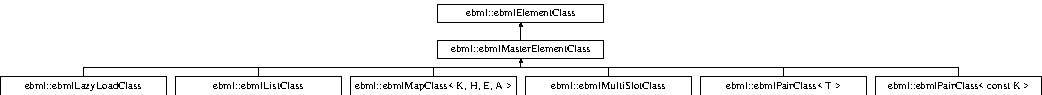
\includegraphics[height=1.534247cm]{classebml_1_1ebmlMasterElementClass}
\end{center}
\end{figure}
\subsection*{Public Member Functions}
\begin{DoxyCompactItemize}
\item 
\mbox{\hyperlink{classebml_1_1ebmlMasterElementClass_a46fb45335e35139c7f694ce9bc247d35}{ebml\+Master\+Element\+Class}} (const char $\ast$, const std\+::wstring \&)
\item 
\mbox{\hyperlink{classebml_1_1ebmlMasterElementClass_a1b455da9db4baed8bfeb2af3a1f7969b}{ebml\+Master\+Element\+Class}} (\mbox{\hyperlink{namespaceebml_a86c5f604ddf12a74aa9812e997a58691}{ebml\+I\+D\+\_\+t}}, const std\+::wstring \&)
\item 
const \mbox{\hyperlink{classebml_1_1childClassSpec__t}{child\+Class\+Spec\+\_\+t}} \& \mbox{\hyperlink{classebml_1_1ebmlMasterElementClass_ab3d49576f8ac2963fa5b996d692175ab}{child\+Classes}} () const
\end{DoxyCompactItemize}
\subsection*{Protected Attributes}
\begin{DoxyCompactItemize}
\item 
\mbox{\hyperlink{classebml_1_1childClassSpec__t}{child\+Class\+Spec\+\_\+t}} \mbox{\hyperlink{classebml_1_1ebmlMasterElementClass_a2281bbfd89c6c3201c1b778efd428cb7}{\+\_\+child\+Classes}}
\end{DoxyCompactItemize}
\subsection*{Friends}
\begin{DoxyCompactItemize}
\item 
class \mbox{\hyperlink{classebml_1_1ebmlMasterElementClass_ad88e86cba72e9332a4693c1c6009b281}{ebml\+Master\+Element}}
\end{DoxyCompactItemize}
\subsection*{Additional Inherited Members}


\subsection{Constructor \& Destructor Documentation}
\mbox{\Hypertarget{classebml_1_1ebmlMasterElementClass_a46fb45335e35139c7f694ce9bc247d35}\label{classebml_1_1ebmlMasterElementClass_a46fb45335e35139c7f694ce9bc247d35}} 
\index{ebml\+::ebml\+Master\+Element\+Class@{ebml\+::ebml\+Master\+Element\+Class}!ebml\+Master\+Element\+Class@{ebml\+Master\+Element\+Class}}
\index{ebml\+Master\+Element\+Class@{ebml\+Master\+Element\+Class}!ebml\+::ebml\+Master\+Element\+Class@{ebml\+::ebml\+Master\+Element\+Class}}
\subsubsection{\texorpdfstring{ebml\+Master\+Element\+Class()}{ebmlMasterElementClass()}\hspace{0.1cm}{\footnotesize\ttfamily [1/2]}}
{\footnotesize\ttfamily ebml\+::ebml\+Master\+Element\+Class\+::ebml\+Master\+Element\+Class (\begin{DoxyParamCaption}\item[{const char $\ast$}]{,  }\item[{const std\+::wstring \&}]{ }\end{DoxyParamCaption})}

\mbox{\Hypertarget{classebml_1_1ebmlMasterElementClass_a1b455da9db4baed8bfeb2af3a1f7969b}\label{classebml_1_1ebmlMasterElementClass_a1b455da9db4baed8bfeb2af3a1f7969b}} 
\index{ebml\+::ebml\+Master\+Element\+Class@{ebml\+::ebml\+Master\+Element\+Class}!ebml\+Master\+Element\+Class@{ebml\+Master\+Element\+Class}}
\index{ebml\+Master\+Element\+Class@{ebml\+Master\+Element\+Class}!ebml\+::ebml\+Master\+Element\+Class@{ebml\+::ebml\+Master\+Element\+Class}}
\subsubsection{\texorpdfstring{ebml\+Master\+Element\+Class()}{ebmlMasterElementClass()}\hspace{0.1cm}{\footnotesize\ttfamily [2/2]}}
{\footnotesize\ttfamily ebml\+::ebml\+Master\+Element\+Class\+::ebml\+Master\+Element\+Class (\begin{DoxyParamCaption}\item[{\mbox{\hyperlink{namespaceebml_a86c5f604ddf12a74aa9812e997a58691}{ebml\+I\+D\+\_\+t}}}]{,  }\item[{const std\+::wstring \&}]{ }\end{DoxyParamCaption})}



\subsection{Member Function Documentation}
\mbox{\Hypertarget{classebml_1_1ebmlMasterElementClass_ab3d49576f8ac2963fa5b996d692175ab}\label{classebml_1_1ebmlMasterElementClass_ab3d49576f8ac2963fa5b996d692175ab}} 
\index{ebml\+::ebml\+Master\+Element\+Class@{ebml\+::ebml\+Master\+Element\+Class}!child\+Classes@{child\+Classes}}
\index{child\+Classes@{child\+Classes}!ebml\+::ebml\+Master\+Element\+Class@{ebml\+::ebml\+Master\+Element\+Class}}
\subsubsection{\texorpdfstring{child\+Classes()}{childClasses()}}
{\footnotesize\ttfamily const \mbox{\hyperlink{classebml_1_1childClassSpec__t}{child\+Class\+Spec\+\_\+t}}\& ebml\+::ebml\+Master\+Element\+Class\+::child\+Classes (\begin{DoxyParamCaption}{ }\end{DoxyParamCaption}) const}



\subsection{Friends And Related Function Documentation}
\mbox{\Hypertarget{classebml_1_1ebmlMasterElementClass_ad88e86cba72e9332a4693c1c6009b281}\label{classebml_1_1ebmlMasterElementClass_ad88e86cba72e9332a4693c1c6009b281}} 
\index{ebml\+::ebml\+Master\+Element\+Class@{ebml\+::ebml\+Master\+Element\+Class}!ebml\+Master\+Element@{ebml\+Master\+Element}}
\index{ebml\+Master\+Element@{ebml\+Master\+Element}!ebml\+::ebml\+Master\+Element\+Class@{ebml\+::ebml\+Master\+Element\+Class}}
\subsubsection{\texorpdfstring{ebml\+Master\+Element}{ebmlMasterElement}}
{\footnotesize\ttfamily friend class \mbox{\hyperlink{classebml_1_1ebmlMasterElement}{ebml\+Master\+Element}}\hspace{0.3cm}{\ttfamily [friend]}}



\subsection{Member Data Documentation}
\mbox{\Hypertarget{classebml_1_1ebmlMasterElementClass_a2281bbfd89c6c3201c1b778efd428cb7}\label{classebml_1_1ebmlMasterElementClass_a2281bbfd89c6c3201c1b778efd428cb7}} 
\index{ebml\+::ebml\+Master\+Element\+Class@{ebml\+::ebml\+Master\+Element\+Class}!\+\_\+child\+Classes@{\+\_\+child\+Classes}}
\index{\+\_\+child\+Classes@{\+\_\+child\+Classes}!ebml\+::ebml\+Master\+Element\+Class@{ebml\+::ebml\+Master\+Element\+Class}}
\subsubsection{\texorpdfstring{\+\_\+child\+Classes}{\_childClasses}}
{\footnotesize\ttfamily \mbox{\hyperlink{classebml_1_1childClassSpec__t}{child\+Class\+Spec\+\_\+t}} ebml\+::ebml\+Master\+Element\+Class\+::\+\_\+child\+Classes\hspace{0.3cm}{\ttfamily [protected]}}



The documentation for this class was generated from the following file\+:\begin{DoxyCompactItemize}
\item 
include/libebml\+\_\+ng/masterelement/\mbox{\hyperlink{masterelement_2base_8h}{base.\+h}}\end{DoxyCompactItemize}

\hypertarget{classebml_1_1ebmlMultiSlot}{}\section{ebml\+:\+:ebml\+Multi\+Slot Class Reference}
\label{classebml_1_1ebmlMultiSlot}\index{ebml\+::ebml\+Multi\+Slot@{ebml\+::ebml\+Multi\+Slot}}


{\ttfamily \#include $<$multislot.\+h$>$}

Inheritance diagram for ebml\+:\+:ebml\+Multi\+Slot\+:\begin{figure}[H]
\begin{center}
\leavevmode
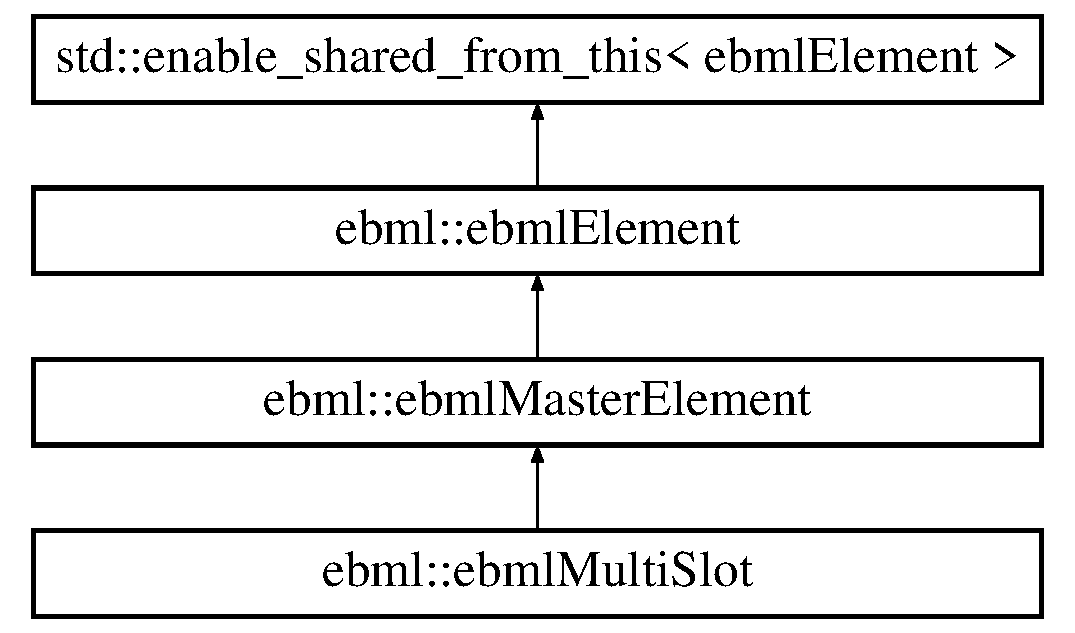
\includegraphics[height=4.000000cm]{classebml_1_1ebmlMultiSlot}
\end{center}
\end{figure}
\subsection*{Classes}
\begin{DoxyCompactItemize}
\item 
class \mbox{\hyperlink{classebml_1_1ebmlMultiSlot_1_1__const__iterator}{\+\_\+const\+\_\+iterator}}
\item 
class \mbox{\hyperlink{classebml_1_1ebmlMultiSlot_1_1__iterator}{\+\_\+iterator}}
\end{DoxyCompactItemize}
\subsection*{Public Member Functions}
\begin{DoxyCompactItemize}
\item 
void \mbox{\hyperlink{classebml_1_1ebmlMultiSlot_afc98f8c3edbde97ecab662c8e9497335}{set\+Data}} (const \mbox{\hyperlink{namespaceebml_ae432575dfbb3e141ce897442794f0ca5}{slot\+Arg\+\_\+l}} \&)
\item 
void \mbox{\hyperlink{classebml_1_1ebmlMultiSlot_aa849380ecfe72c8e13b0ec62ce1eee5d}{set\+Data}} (\mbox{\hyperlink{namespaceebml_ae432575dfbb3e141ce897442794f0ca5}{slot\+Arg\+\_\+l}} \&\&)
\item 
void \mbox{\hyperlink{classebml_1_1ebmlMultiSlot_a26efa69855cf4e6ce5d220a90f5bc55b}{set\+Data}} (const \mbox{\hyperlink{namespaceebml_a4317d4c495715eced3ed448c2d05caeb}{slot\+Arg\+\_\+d}} \&)
\item 
void \mbox{\hyperlink{classebml_1_1ebmlMultiSlot_ae5c436b93c6f810bceda911890606e88}{set\+Data}} (\mbox{\hyperlink{namespaceebml_a4317d4c495715eced3ed448c2d05caeb}{slot\+Arg\+\_\+d}} \&\&)
\item 
void \mbox{\hyperlink{classebml_1_1ebmlMultiSlot_a8a54cc97efcae5cad451703f1e95f82e}{set\+Data}} (const \mbox{\hyperlink{namespaceebml_ae432575dfbb3e141ce897442794f0ca5}{slot\+Arg\+\_\+l}} \&, const \mbox{\hyperlink{namespaceebml_a4317d4c495715eced3ed448c2d05caeb}{slot\+Arg\+\_\+d}} \&)
\item 
void \mbox{\hyperlink{classebml_1_1ebmlMultiSlot_a762c96dfeff8e877b6c9d40fdda6d0d2}{set\+Data}} (\mbox{\hyperlink{namespaceebml_ae432575dfbb3e141ce897442794f0ca5}{slot\+Arg\+\_\+l}} \&\&, \mbox{\hyperlink{namespaceebml_a4317d4c495715eced3ed448c2d05caeb}{slot\+Arg\+\_\+d}} \&\&)
\item 
std\+::wstring \mbox{\hyperlink{classebml_1_1ebmlMultiSlot_a3a2407406cd68f27d974cc18223c86c0}{minirepr}} () const override
\item 
\mbox{\hyperlink{classebml_1_1slot__t}{slot\+\_\+t}} \mbox{\hyperlink{classebml_1_1ebmlMultiSlot_a9edb99f1fd34d4ba765fa5f1266026ec}{operator\mbox{[}$\,$\mbox{]}}} (size\+\_\+t)
\item 
\mbox{\hyperlink{classebml_1_1slot__t}{slot\+\_\+t}} \mbox{\hyperlink{classebml_1_1ebmlMultiSlot_aee35de0e28c6e7916951d6094576b639}{operator\mbox{[}$\,$\mbox{]}}} (const std\+::string \&)
\item 
\mbox{\hyperlink{classebml_1_1const__slot__t}{const\+\_\+slot\+\_\+t}} \mbox{\hyperlink{classebml_1_1ebmlMultiSlot_a82a094d9159d4c527ac265dbb0852905}{operator\mbox{[}$\,$\mbox{]}}} (size\+\_\+t) const
\item 
\mbox{\hyperlink{classebml_1_1const__slot__t}{const\+\_\+slot\+\_\+t}} \mbox{\hyperlink{classebml_1_1ebmlMultiSlot_ac8b464bc8f1aecd2f491217448d547e8}{operator\mbox{[}$\,$\mbox{]}}} (const std\+::string \&) const
\end{DoxyCompactItemize}
\subsection*{Protected Member Functions}
\begin{DoxyCompactItemize}
\item 
\mbox{\hyperlink{classebml_1_1ebmlMultiSlot_a736f14f96d3a2f8b288e984113c86c9b}{ebml\+Multi\+Slot}} (const \mbox{\hyperlink{classebml_1_1ebmlMultiSlotClass}{ebml\+Multi\+Slot\+Class}} $\ast$)
\item 
void \mbox{\hyperlink{classebml_1_1ebmlMultiSlot_a0743d6fcdd75068045d53397c97dd2c3}{\+\_\+clear}} () override
\item 
void \mbox{\hyperlink{classebml_1_1ebmlMultiSlot_af6377e38bc00a9ac5a6af007644e0f66}{\+\_\+validate\+Args}} (const \mbox{\hyperlink{namespaceebml_ae432575dfbb3e141ce897442794f0ca5}{slot\+Arg\+\_\+l}} \&args)
\item 
void \mbox{\hyperlink{classebml_1_1ebmlMultiSlot_a96fb07cd63255265521772ce0080c3cb}{\+\_\+validate\+Args}} (const \mbox{\hyperlink{namespaceebml_a4317d4c495715eced3ed448c2d05caeb}{slot\+Arg\+\_\+d}} \&kwargs)
\item 
void \mbox{\hyperlink{classebml_1_1ebmlMultiSlot_ae405c0712f66903b2f05b74132eb1317}{\+\_\+validate\+Args}} (const \mbox{\hyperlink{namespaceebml_ae432575dfbb3e141ce897442794f0ca5}{slot\+Arg\+\_\+l}} \&args, const \mbox{\hyperlink{namespaceebml_a4317d4c495715eced3ed448c2d05caeb}{slot\+Arg\+\_\+d}} \&kwargs)
\item 
void \mbox{\hyperlink{classebml_1_1ebmlMultiSlot_a55c35fb4ca640b362e395515088140eb}{\+\_\+validate\+Data}} (const \mbox{\hyperlink{namespaceebml_ae432575dfbb3e141ce897442794f0ca5}{slot\+Arg\+\_\+l}} \&args)
\item 
void \mbox{\hyperlink{classebml_1_1ebmlMultiSlot_a4c3233d2c54713803d113d6bed9b4663}{\+\_\+validate\+Data}} (const \mbox{\hyperlink{namespaceebml_a4317d4c495715eced3ed448c2d05caeb}{slot\+Arg\+\_\+d}} \&args)
\item 
void \mbox{\hyperlink{classebml_1_1ebmlMultiSlot_a35a5efc5bb9dcc976bec3d4be4303925}{\+\_\+set\+Data}} (const \mbox{\hyperlink{namespaceebml_ae432575dfbb3e141ce897442794f0ca5}{slot\+Arg\+\_\+l}} \&args)
\item 
void \mbox{\hyperlink{classebml_1_1ebmlMultiSlot_a5113a76cfd5de57c83b6ecb2f459d848}{\+\_\+set\+Data}} (\mbox{\hyperlink{namespaceebml_ae432575dfbb3e141ce897442794f0ca5}{slot\+Arg\+\_\+l}} \&\&args)
\item 
void \mbox{\hyperlink{classebml_1_1ebmlMultiSlot_ada5486b817bc70eaaebec2cd80c8ecf1}{\+\_\+set\+Data}} (const \mbox{\hyperlink{namespaceebml_a4317d4c495715eced3ed448c2d05caeb}{slot\+Arg\+\_\+d}} \&kwargs)
\item 
void \mbox{\hyperlink{classebml_1_1ebmlMultiSlot_a3de8d499755f77822a4b135f37741bb9}{\+\_\+set\+Data}} (\mbox{\hyperlink{namespaceebml_a4317d4c495715eced3ed448c2d05caeb}{slot\+Arg\+\_\+d}} \&\&kwargs)
\item 
\mbox{\hyperlink{classebml_1_1ebmlMasterElement_1_1__iterator}{ebml\+Master\+Element\+::\+\_\+iterator}} $\ast$ \mbox{\hyperlink{classebml_1_1ebmlMultiSlot_a61a2bb09ccbf771a9023774e0cdcbad2}{\+\_\+begin}} () override
\item 
\mbox{\hyperlink{classebml_1_1ebmlMasterElement_1_1__iterator}{ebml\+Master\+Element\+::\+\_\+iterator}} $\ast$ \mbox{\hyperlink{classebml_1_1ebmlMultiSlot_a8374290bfe21447729ed0331eb845905}{\+\_\+end}} () override
\item 
\mbox{\hyperlink{classebml_1_1ebmlMasterElement_1_1__const__iterator}{ebml\+Master\+Element\+::\+\_\+const\+\_\+iterator}} $\ast$ \mbox{\hyperlink{classebml_1_1ebmlMultiSlot_adf1816c367909a1d265f38419febf9c7}{\+\_\+cbegin}} () const override
\item 
\mbox{\hyperlink{classebml_1_1ebmlMasterElement_1_1__const__iterator}{ebml\+Master\+Element\+::\+\_\+const\+\_\+iterator}} $\ast$ \mbox{\hyperlink{classebml_1_1ebmlMultiSlot_a6bc62e4030734829022930e89e94278e}{\+\_\+cend}} () const override
\item 
void \mbox{\hyperlink{classebml_1_1ebmlMultiSlot_ad5f24ddcacb5a5fcc78a8cc50166d092}{\+\_\+add\+Child}} (const \mbox{\hyperlink{namespaceebml_adad533b7705a16bb360fe56380c5e7be}{ebml\+Element\+\_\+sp}} \&) override
\item 
void \mbox{\hyperlink{classebml_1_1ebmlMultiSlot_aa8d38591ef1932423e2f62d42cc4967c}{\+\_\+add\+Child}} (\mbox{\hyperlink{namespaceebml_adad533b7705a16bb360fe56380c5e7be}{ebml\+Element\+\_\+sp}} \&\&) override
\end{DoxyCompactItemize}
\subsection*{Friends}
\begin{DoxyCompactItemize}
\item 
class \mbox{\hyperlink{classebml_1_1ebmlMultiSlot_a229e8a019ffa3d8ab84c711635badcd1}{ebml\+Multi\+Slot\+Class}}
\item 
class \mbox{\hyperlink{classebml_1_1ebmlMultiSlot_a6546cbde3dc2846c329fd0ea73da851b}{slot\+\_\+t}}
\end{DoxyCompactItemize}
\subsection*{Additional Inherited Members}


\subsection{Constructor \& Destructor Documentation}
\mbox{\Hypertarget{classebml_1_1ebmlMultiSlot_a736f14f96d3a2f8b288e984113c86c9b}\label{classebml_1_1ebmlMultiSlot_a736f14f96d3a2f8b288e984113c86c9b}} 
\index{ebml\+::ebml\+Multi\+Slot@{ebml\+::ebml\+Multi\+Slot}!ebml\+Multi\+Slot@{ebml\+Multi\+Slot}}
\index{ebml\+Multi\+Slot@{ebml\+Multi\+Slot}!ebml\+::ebml\+Multi\+Slot@{ebml\+::ebml\+Multi\+Slot}}
\subsubsection{\texorpdfstring{ebml\+Multi\+Slot()}{ebmlMultiSlot()}}
{\footnotesize\ttfamily ebml\+::ebml\+Multi\+Slot\+::ebml\+Multi\+Slot (\begin{DoxyParamCaption}\item[{const \mbox{\hyperlink{classebml_1_1ebmlMultiSlotClass}{ebml\+Multi\+Slot\+Class}} $\ast$}]{ }\end{DoxyParamCaption})\hspace{0.3cm}{\ttfamily [protected]}}



\subsection{Member Function Documentation}
\mbox{\Hypertarget{classebml_1_1ebmlMultiSlot_ad5f24ddcacb5a5fcc78a8cc50166d092}\label{classebml_1_1ebmlMultiSlot_ad5f24ddcacb5a5fcc78a8cc50166d092}} 
\index{ebml\+::ebml\+Multi\+Slot@{ebml\+::ebml\+Multi\+Slot}!\+\_\+add\+Child@{\+\_\+add\+Child}}
\index{\+\_\+add\+Child@{\+\_\+add\+Child}!ebml\+::ebml\+Multi\+Slot@{ebml\+::ebml\+Multi\+Slot}}
\subsubsection{\texorpdfstring{\+\_\+add\+Child()}{\_addChild()}\hspace{0.1cm}{\footnotesize\ttfamily [1/2]}}
{\footnotesize\ttfamily void ebml\+::ebml\+Multi\+Slot\+::\+\_\+add\+Child (\begin{DoxyParamCaption}\item[{const \mbox{\hyperlink{namespaceebml_adad533b7705a16bb360fe56380c5e7be}{ebml\+Element\+\_\+sp}} \&}]{ }\end{DoxyParamCaption})\hspace{0.3cm}{\ttfamily [override]}, {\ttfamily [protected]}, {\ttfamily [virtual]}}



Implements \mbox{\hyperlink{classebml_1_1ebmlMasterElement_a59c5f3b3409fd5fd6f0f22c7a68f1c9b}{ebml\+::ebml\+Master\+Element}}.

\mbox{\Hypertarget{classebml_1_1ebmlMultiSlot_aa8d38591ef1932423e2f62d42cc4967c}\label{classebml_1_1ebmlMultiSlot_aa8d38591ef1932423e2f62d42cc4967c}} 
\index{ebml\+::ebml\+Multi\+Slot@{ebml\+::ebml\+Multi\+Slot}!\+\_\+add\+Child@{\+\_\+add\+Child}}
\index{\+\_\+add\+Child@{\+\_\+add\+Child}!ebml\+::ebml\+Multi\+Slot@{ebml\+::ebml\+Multi\+Slot}}
\subsubsection{\texorpdfstring{\+\_\+add\+Child()}{\_addChild()}\hspace{0.1cm}{\footnotesize\ttfamily [2/2]}}
{\footnotesize\ttfamily void ebml\+::ebml\+Multi\+Slot\+::\+\_\+add\+Child (\begin{DoxyParamCaption}\item[{\mbox{\hyperlink{namespaceebml_adad533b7705a16bb360fe56380c5e7be}{ebml\+Element\+\_\+sp}} \&\&}]{ }\end{DoxyParamCaption})\hspace{0.3cm}{\ttfamily [override]}, {\ttfamily [protected]}, {\ttfamily [virtual]}}



Implements \mbox{\hyperlink{classebml_1_1ebmlMasterElement_a3af0270846a1ced1719d26dd261f0355}{ebml\+::ebml\+Master\+Element}}.

\mbox{\Hypertarget{classebml_1_1ebmlMultiSlot_a61a2bb09ccbf771a9023774e0cdcbad2}\label{classebml_1_1ebmlMultiSlot_a61a2bb09ccbf771a9023774e0cdcbad2}} 
\index{ebml\+::ebml\+Multi\+Slot@{ebml\+::ebml\+Multi\+Slot}!\+\_\+begin@{\+\_\+begin}}
\index{\+\_\+begin@{\+\_\+begin}!ebml\+::ebml\+Multi\+Slot@{ebml\+::ebml\+Multi\+Slot}}
\subsubsection{\texorpdfstring{\+\_\+begin()}{\_begin()}}
{\footnotesize\ttfamily \mbox{\hyperlink{classebml_1_1ebmlMasterElement_1_1__iterator}{ebml\+Master\+Element\+::\+\_\+iterator}}$\ast$ ebml\+::ebml\+Multi\+Slot\+::\+\_\+begin (\begin{DoxyParamCaption}{ }\end{DoxyParamCaption})\hspace{0.3cm}{\ttfamily [override]}, {\ttfamily [protected]}, {\ttfamily [virtual]}}



Implements \mbox{\hyperlink{classebml_1_1ebmlMasterElement_af6fb7a9934e9b8d0c64273ef6944f44b}{ebml\+::ebml\+Master\+Element}}.

\mbox{\Hypertarget{classebml_1_1ebmlMultiSlot_adf1816c367909a1d265f38419febf9c7}\label{classebml_1_1ebmlMultiSlot_adf1816c367909a1d265f38419febf9c7}} 
\index{ebml\+::ebml\+Multi\+Slot@{ebml\+::ebml\+Multi\+Slot}!\+\_\+cbegin@{\+\_\+cbegin}}
\index{\+\_\+cbegin@{\+\_\+cbegin}!ebml\+::ebml\+Multi\+Slot@{ebml\+::ebml\+Multi\+Slot}}
\subsubsection{\texorpdfstring{\+\_\+cbegin()}{\_cbegin()}}
{\footnotesize\ttfamily \mbox{\hyperlink{classebml_1_1ebmlMasterElement_1_1__const__iterator}{ebml\+Master\+Element\+::\+\_\+const\+\_\+iterator}}$\ast$ ebml\+::ebml\+Multi\+Slot\+::\+\_\+cbegin (\begin{DoxyParamCaption}{ }\end{DoxyParamCaption}) const\hspace{0.3cm}{\ttfamily [override]}, {\ttfamily [protected]}, {\ttfamily [virtual]}}



Implements \mbox{\hyperlink{classebml_1_1ebmlMasterElement_a7e1ffa498e22b637a6671df14aa0bc45}{ebml\+::ebml\+Master\+Element}}.

\mbox{\Hypertarget{classebml_1_1ebmlMultiSlot_a6bc62e4030734829022930e89e94278e}\label{classebml_1_1ebmlMultiSlot_a6bc62e4030734829022930e89e94278e}} 
\index{ebml\+::ebml\+Multi\+Slot@{ebml\+::ebml\+Multi\+Slot}!\+\_\+cend@{\+\_\+cend}}
\index{\+\_\+cend@{\+\_\+cend}!ebml\+::ebml\+Multi\+Slot@{ebml\+::ebml\+Multi\+Slot}}
\subsubsection{\texorpdfstring{\+\_\+cend()}{\_cend()}}
{\footnotesize\ttfamily \mbox{\hyperlink{classebml_1_1ebmlMasterElement_1_1__const__iterator}{ebml\+Master\+Element\+::\+\_\+const\+\_\+iterator}}$\ast$ ebml\+::ebml\+Multi\+Slot\+::\+\_\+cend (\begin{DoxyParamCaption}{ }\end{DoxyParamCaption}) const\hspace{0.3cm}{\ttfamily [override]}, {\ttfamily [protected]}, {\ttfamily [virtual]}}



Implements \mbox{\hyperlink{classebml_1_1ebmlMasterElement_ae6cdbf68d8267a7ab098bd402fa70e88}{ebml\+::ebml\+Master\+Element}}.

\mbox{\Hypertarget{classebml_1_1ebmlMultiSlot_a0743d6fcdd75068045d53397c97dd2c3}\label{classebml_1_1ebmlMultiSlot_a0743d6fcdd75068045d53397c97dd2c3}} 
\index{ebml\+::ebml\+Multi\+Slot@{ebml\+::ebml\+Multi\+Slot}!\+\_\+clear@{\+\_\+clear}}
\index{\+\_\+clear@{\+\_\+clear}!ebml\+::ebml\+Multi\+Slot@{ebml\+::ebml\+Multi\+Slot}}
\subsubsection{\texorpdfstring{\+\_\+clear()}{\_clear()}}
{\footnotesize\ttfamily void ebml\+::ebml\+Multi\+Slot\+::\+\_\+clear (\begin{DoxyParamCaption}{ }\end{DoxyParamCaption})\hspace{0.3cm}{\ttfamily [override]}, {\ttfamily [protected]}, {\ttfamily [virtual]}}



Reimplemented from \mbox{\hyperlink{classebml_1_1ebmlMasterElement_a2fdf9fa1022f06a046fe94e631e266a3}{ebml\+::ebml\+Master\+Element}}.

\mbox{\Hypertarget{classebml_1_1ebmlMultiSlot_a8374290bfe21447729ed0331eb845905}\label{classebml_1_1ebmlMultiSlot_a8374290bfe21447729ed0331eb845905}} 
\index{ebml\+::ebml\+Multi\+Slot@{ebml\+::ebml\+Multi\+Slot}!\+\_\+end@{\+\_\+end}}
\index{\+\_\+end@{\+\_\+end}!ebml\+::ebml\+Multi\+Slot@{ebml\+::ebml\+Multi\+Slot}}
\subsubsection{\texorpdfstring{\+\_\+end()}{\_end()}}
{\footnotesize\ttfamily \mbox{\hyperlink{classebml_1_1ebmlMasterElement_1_1__iterator}{ebml\+Master\+Element\+::\+\_\+iterator}}$\ast$ ebml\+::ebml\+Multi\+Slot\+::\+\_\+end (\begin{DoxyParamCaption}{ }\end{DoxyParamCaption})\hspace{0.3cm}{\ttfamily [override]}, {\ttfamily [protected]}, {\ttfamily [virtual]}}



Implements \mbox{\hyperlink{classebml_1_1ebmlMasterElement_a352e5e11836063394990cb05c09d8e48}{ebml\+::ebml\+Master\+Element}}.

\mbox{\Hypertarget{classebml_1_1ebmlMultiSlot_a35a5efc5bb9dcc976bec3d4be4303925}\label{classebml_1_1ebmlMultiSlot_a35a5efc5bb9dcc976bec3d4be4303925}} 
\index{ebml\+::ebml\+Multi\+Slot@{ebml\+::ebml\+Multi\+Slot}!\+\_\+set\+Data@{\+\_\+set\+Data}}
\index{\+\_\+set\+Data@{\+\_\+set\+Data}!ebml\+::ebml\+Multi\+Slot@{ebml\+::ebml\+Multi\+Slot}}
\subsubsection{\texorpdfstring{\+\_\+set\+Data()}{\_setData()}\hspace{0.1cm}{\footnotesize\ttfamily [1/4]}}
{\footnotesize\ttfamily void ebml\+::ebml\+Multi\+Slot\+::\+\_\+set\+Data (\begin{DoxyParamCaption}\item[{const \mbox{\hyperlink{namespaceebml_ae432575dfbb3e141ce897442794f0ca5}{slot\+Arg\+\_\+l}} \&}]{args }\end{DoxyParamCaption})\hspace{0.3cm}{\ttfamily [protected]}}

\mbox{\Hypertarget{classebml_1_1ebmlMultiSlot_a5113a76cfd5de57c83b6ecb2f459d848}\label{classebml_1_1ebmlMultiSlot_a5113a76cfd5de57c83b6ecb2f459d848}} 
\index{ebml\+::ebml\+Multi\+Slot@{ebml\+::ebml\+Multi\+Slot}!\+\_\+set\+Data@{\+\_\+set\+Data}}
\index{\+\_\+set\+Data@{\+\_\+set\+Data}!ebml\+::ebml\+Multi\+Slot@{ebml\+::ebml\+Multi\+Slot}}
\subsubsection{\texorpdfstring{\+\_\+set\+Data()}{\_setData()}\hspace{0.1cm}{\footnotesize\ttfamily [2/4]}}
{\footnotesize\ttfamily void ebml\+::ebml\+Multi\+Slot\+::\+\_\+set\+Data (\begin{DoxyParamCaption}\item[{\mbox{\hyperlink{namespaceebml_ae432575dfbb3e141ce897442794f0ca5}{slot\+Arg\+\_\+l}} \&\&}]{args }\end{DoxyParamCaption})\hspace{0.3cm}{\ttfamily [protected]}}

\mbox{\Hypertarget{classebml_1_1ebmlMultiSlot_ada5486b817bc70eaaebec2cd80c8ecf1}\label{classebml_1_1ebmlMultiSlot_ada5486b817bc70eaaebec2cd80c8ecf1}} 
\index{ebml\+::ebml\+Multi\+Slot@{ebml\+::ebml\+Multi\+Slot}!\+\_\+set\+Data@{\+\_\+set\+Data}}
\index{\+\_\+set\+Data@{\+\_\+set\+Data}!ebml\+::ebml\+Multi\+Slot@{ebml\+::ebml\+Multi\+Slot}}
\subsubsection{\texorpdfstring{\+\_\+set\+Data()}{\_setData()}\hspace{0.1cm}{\footnotesize\ttfamily [3/4]}}
{\footnotesize\ttfamily void ebml\+::ebml\+Multi\+Slot\+::\+\_\+set\+Data (\begin{DoxyParamCaption}\item[{const \mbox{\hyperlink{namespaceebml_a4317d4c495715eced3ed448c2d05caeb}{slot\+Arg\+\_\+d}} \&}]{kwargs }\end{DoxyParamCaption})\hspace{0.3cm}{\ttfamily [protected]}}

\mbox{\Hypertarget{classebml_1_1ebmlMultiSlot_a3de8d499755f77822a4b135f37741bb9}\label{classebml_1_1ebmlMultiSlot_a3de8d499755f77822a4b135f37741bb9}} 
\index{ebml\+::ebml\+Multi\+Slot@{ebml\+::ebml\+Multi\+Slot}!\+\_\+set\+Data@{\+\_\+set\+Data}}
\index{\+\_\+set\+Data@{\+\_\+set\+Data}!ebml\+::ebml\+Multi\+Slot@{ebml\+::ebml\+Multi\+Slot}}
\subsubsection{\texorpdfstring{\+\_\+set\+Data()}{\_setData()}\hspace{0.1cm}{\footnotesize\ttfamily [4/4]}}
{\footnotesize\ttfamily void ebml\+::ebml\+Multi\+Slot\+::\+\_\+set\+Data (\begin{DoxyParamCaption}\item[{\mbox{\hyperlink{namespaceebml_a4317d4c495715eced3ed448c2d05caeb}{slot\+Arg\+\_\+d}} \&\&}]{kwargs }\end{DoxyParamCaption})\hspace{0.3cm}{\ttfamily [protected]}}

\mbox{\Hypertarget{classebml_1_1ebmlMultiSlot_af6377e38bc00a9ac5a6af007644e0f66}\label{classebml_1_1ebmlMultiSlot_af6377e38bc00a9ac5a6af007644e0f66}} 
\index{ebml\+::ebml\+Multi\+Slot@{ebml\+::ebml\+Multi\+Slot}!\+\_\+validate\+Args@{\+\_\+validate\+Args}}
\index{\+\_\+validate\+Args@{\+\_\+validate\+Args}!ebml\+::ebml\+Multi\+Slot@{ebml\+::ebml\+Multi\+Slot}}
\subsubsection{\texorpdfstring{\+\_\+validate\+Args()}{\_validateArgs()}\hspace{0.1cm}{\footnotesize\ttfamily [1/3]}}
{\footnotesize\ttfamily void ebml\+::ebml\+Multi\+Slot\+::\+\_\+validate\+Args (\begin{DoxyParamCaption}\item[{const \mbox{\hyperlink{namespaceebml_ae432575dfbb3e141ce897442794f0ca5}{slot\+Arg\+\_\+l}} \&}]{args }\end{DoxyParamCaption})\hspace{0.3cm}{\ttfamily [protected]}}

\mbox{\Hypertarget{classebml_1_1ebmlMultiSlot_a96fb07cd63255265521772ce0080c3cb}\label{classebml_1_1ebmlMultiSlot_a96fb07cd63255265521772ce0080c3cb}} 
\index{ebml\+::ebml\+Multi\+Slot@{ebml\+::ebml\+Multi\+Slot}!\+\_\+validate\+Args@{\+\_\+validate\+Args}}
\index{\+\_\+validate\+Args@{\+\_\+validate\+Args}!ebml\+::ebml\+Multi\+Slot@{ebml\+::ebml\+Multi\+Slot}}
\subsubsection{\texorpdfstring{\+\_\+validate\+Args()}{\_validateArgs()}\hspace{0.1cm}{\footnotesize\ttfamily [2/3]}}
{\footnotesize\ttfamily void ebml\+::ebml\+Multi\+Slot\+::\+\_\+validate\+Args (\begin{DoxyParamCaption}\item[{const \mbox{\hyperlink{namespaceebml_a4317d4c495715eced3ed448c2d05caeb}{slot\+Arg\+\_\+d}} \&}]{kwargs }\end{DoxyParamCaption})\hspace{0.3cm}{\ttfamily [protected]}}

\mbox{\Hypertarget{classebml_1_1ebmlMultiSlot_ae405c0712f66903b2f05b74132eb1317}\label{classebml_1_1ebmlMultiSlot_ae405c0712f66903b2f05b74132eb1317}} 
\index{ebml\+::ebml\+Multi\+Slot@{ebml\+::ebml\+Multi\+Slot}!\+\_\+validate\+Args@{\+\_\+validate\+Args}}
\index{\+\_\+validate\+Args@{\+\_\+validate\+Args}!ebml\+::ebml\+Multi\+Slot@{ebml\+::ebml\+Multi\+Slot}}
\subsubsection{\texorpdfstring{\+\_\+validate\+Args()}{\_validateArgs()}\hspace{0.1cm}{\footnotesize\ttfamily [3/3]}}
{\footnotesize\ttfamily void ebml\+::ebml\+Multi\+Slot\+::\+\_\+validate\+Args (\begin{DoxyParamCaption}\item[{const \mbox{\hyperlink{namespaceebml_ae432575dfbb3e141ce897442794f0ca5}{slot\+Arg\+\_\+l}} \&}]{args,  }\item[{const \mbox{\hyperlink{namespaceebml_a4317d4c495715eced3ed448c2d05caeb}{slot\+Arg\+\_\+d}} \&}]{kwargs }\end{DoxyParamCaption})\hspace{0.3cm}{\ttfamily [protected]}}

\mbox{\Hypertarget{classebml_1_1ebmlMultiSlot_a55c35fb4ca640b362e395515088140eb}\label{classebml_1_1ebmlMultiSlot_a55c35fb4ca640b362e395515088140eb}} 
\index{ebml\+::ebml\+Multi\+Slot@{ebml\+::ebml\+Multi\+Slot}!\+\_\+validate\+Data@{\+\_\+validate\+Data}}
\index{\+\_\+validate\+Data@{\+\_\+validate\+Data}!ebml\+::ebml\+Multi\+Slot@{ebml\+::ebml\+Multi\+Slot}}
\subsubsection{\texorpdfstring{\+\_\+validate\+Data()}{\_validateData()}\hspace{0.1cm}{\footnotesize\ttfamily [1/2]}}
{\footnotesize\ttfamily void ebml\+::ebml\+Multi\+Slot\+::\+\_\+validate\+Data (\begin{DoxyParamCaption}\item[{const \mbox{\hyperlink{namespaceebml_ae432575dfbb3e141ce897442794f0ca5}{slot\+Arg\+\_\+l}} \&}]{args }\end{DoxyParamCaption})\hspace{0.3cm}{\ttfamily [protected]}}

\mbox{\Hypertarget{classebml_1_1ebmlMultiSlot_a4c3233d2c54713803d113d6bed9b4663}\label{classebml_1_1ebmlMultiSlot_a4c3233d2c54713803d113d6bed9b4663}} 
\index{ebml\+::ebml\+Multi\+Slot@{ebml\+::ebml\+Multi\+Slot}!\+\_\+validate\+Data@{\+\_\+validate\+Data}}
\index{\+\_\+validate\+Data@{\+\_\+validate\+Data}!ebml\+::ebml\+Multi\+Slot@{ebml\+::ebml\+Multi\+Slot}}
\subsubsection{\texorpdfstring{\+\_\+validate\+Data()}{\_validateData()}\hspace{0.1cm}{\footnotesize\ttfamily [2/2]}}
{\footnotesize\ttfamily void ebml\+::ebml\+Multi\+Slot\+::\+\_\+validate\+Data (\begin{DoxyParamCaption}\item[{const \mbox{\hyperlink{namespaceebml_a4317d4c495715eced3ed448c2d05caeb}{slot\+Arg\+\_\+d}} \&}]{args }\end{DoxyParamCaption})\hspace{0.3cm}{\ttfamily [protected]}}

\mbox{\Hypertarget{classebml_1_1ebmlMultiSlot_a3a2407406cd68f27d974cc18223c86c0}\label{classebml_1_1ebmlMultiSlot_a3a2407406cd68f27d974cc18223c86c0}} 
\index{ebml\+::ebml\+Multi\+Slot@{ebml\+::ebml\+Multi\+Slot}!minirepr@{minirepr}}
\index{minirepr@{minirepr}!ebml\+::ebml\+Multi\+Slot@{ebml\+::ebml\+Multi\+Slot}}
\subsubsection{\texorpdfstring{minirepr()}{minirepr()}}
{\footnotesize\ttfamily std\+::wstring ebml\+::ebml\+Multi\+Slot\+::minirepr (\begin{DoxyParamCaption}{ }\end{DoxyParamCaption}) const\hspace{0.3cm}{\ttfamily [override]}, {\ttfamily [virtual]}}



Implements \mbox{\hyperlink{classebml_1_1ebmlElement_a7852173aeef78bd843939ae5a82f1d1c}{ebml\+::ebml\+Element}}.

\mbox{\Hypertarget{classebml_1_1ebmlMultiSlot_a9edb99f1fd34d4ba765fa5f1266026ec}\label{classebml_1_1ebmlMultiSlot_a9edb99f1fd34d4ba765fa5f1266026ec}} 
\index{ebml\+::ebml\+Multi\+Slot@{ebml\+::ebml\+Multi\+Slot}!operator\mbox{[}\mbox{]}@{operator[]}}
\index{operator\mbox{[}\mbox{]}@{operator[]}!ebml\+::ebml\+Multi\+Slot@{ebml\+::ebml\+Multi\+Slot}}
\subsubsection{\texorpdfstring{operator[]()}{operator[]()}\hspace{0.1cm}{\footnotesize\ttfamily [1/4]}}
{\footnotesize\ttfamily \mbox{\hyperlink{classebml_1_1slot__t}{slot\+\_\+t}} ebml\+::ebml\+Multi\+Slot\+::operator\mbox{[}$\,$\mbox{]} (\begin{DoxyParamCaption}\item[{size\+\_\+t}]{ }\end{DoxyParamCaption})}

\mbox{\Hypertarget{classebml_1_1ebmlMultiSlot_aee35de0e28c6e7916951d6094576b639}\label{classebml_1_1ebmlMultiSlot_aee35de0e28c6e7916951d6094576b639}} 
\index{ebml\+::ebml\+Multi\+Slot@{ebml\+::ebml\+Multi\+Slot}!operator\mbox{[}\mbox{]}@{operator[]}}
\index{operator\mbox{[}\mbox{]}@{operator[]}!ebml\+::ebml\+Multi\+Slot@{ebml\+::ebml\+Multi\+Slot}}
\subsubsection{\texorpdfstring{operator[]()}{operator[]()}\hspace{0.1cm}{\footnotesize\ttfamily [2/4]}}
{\footnotesize\ttfamily \mbox{\hyperlink{classebml_1_1slot__t}{slot\+\_\+t}} ebml\+::ebml\+Multi\+Slot\+::operator\mbox{[}$\,$\mbox{]} (\begin{DoxyParamCaption}\item[{const std\+::string \&}]{ }\end{DoxyParamCaption})}

\mbox{\Hypertarget{classebml_1_1ebmlMultiSlot_a82a094d9159d4c527ac265dbb0852905}\label{classebml_1_1ebmlMultiSlot_a82a094d9159d4c527ac265dbb0852905}} 
\index{ebml\+::ebml\+Multi\+Slot@{ebml\+::ebml\+Multi\+Slot}!operator\mbox{[}\mbox{]}@{operator[]}}
\index{operator\mbox{[}\mbox{]}@{operator[]}!ebml\+::ebml\+Multi\+Slot@{ebml\+::ebml\+Multi\+Slot}}
\subsubsection{\texorpdfstring{operator[]()}{operator[]()}\hspace{0.1cm}{\footnotesize\ttfamily [3/4]}}
{\footnotesize\ttfamily \mbox{\hyperlink{classebml_1_1const__slot__t}{const\+\_\+slot\+\_\+t}} ebml\+::ebml\+Multi\+Slot\+::operator\mbox{[}$\,$\mbox{]} (\begin{DoxyParamCaption}\item[{size\+\_\+t}]{ }\end{DoxyParamCaption}) const}

\mbox{\Hypertarget{classebml_1_1ebmlMultiSlot_ac8b464bc8f1aecd2f491217448d547e8}\label{classebml_1_1ebmlMultiSlot_ac8b464bc8f1aecd2f491217448d547e8}} 
\index{ebml\+::ebml\+Multi\+Slot@{ebml\+::ebml\+Multi\+Slot}!operator\mbox{[}\mbox{]}@{operator[]}}
\index{operator\mbox{[}\mbox{]}@{operator[]}!ebml\+::ebml\+Multi\+Slot@{ebml\+::ebml\+Multi\+Slot}}
\subsubsection{\texorpdfstring{operator[]()}{operator[]()}\hspace{0.1cm}{\footnotesize\ttfamily [4/4]}}
{\footnotesize\ttfamily \mbox{\hyperlink{classebml_1_1const__slot__t}{const\+\_\+slot\+\_\+t}} ebml\+::ebml\+Multi\+Slot\+::operator\mbox{[}$\,$\mbox{]} (\begin{DoxyParamCaption}\item[{const std\+::string \&}]{ }\end{DoxyParamCaption}) const}

\mbox{\Hypertarget{classebml_1_1ebmlMultiSlot_afc98f8c3edbde97ecab662c8e9497335}\label{classebml_1_1ebmlMultiSlot_afc98f8c3edbde97ecab662c8e9497335}} 
\index{ebml\+::ebml\+Multi\+Slot@{ebml\+::ebml\+Multi\+Slot}!set\+Data@{set\+Data}}
\index{set\+Data@{set\+Data}!ebml\+::ebml\+Multi\+Slot@{ebml\+::ebml\+Multi\+Slot}}
\subsubsection{\texorpdfstring{set\+Data()}{setData()}\hspace{0.1cm}{\footnotesize\ttfamily [1/6]}}
{\footnotesize\ttfamily void ebml\+::ebml\+Multi\+Slot\+::set\+Data (\begin{DoxyParamCaption}\item[{const \mbox{\hyperlink{namespaceebml_ae432575dfbb3e141ce897442794f0ca5}{slot\+Arg\+\_\+l}} \&}]{ }\end{DoxyParamCaption})}

\mbox{\Hypertarget{classebml_1_1ebmlMultiSlot_aa849380ecfe72c8e13b0ec62ce1eee5d}\label{classebml_1_1ebmlMultiSlot_aa849380ecfe72c8e13b0ec62ce1eee5d}} 
\index{ebml\+::ebml\+Multi\+Slot@{ebml\+::ebml\+Multi\+Slot}!set\+Data@{set\+Data}}
\index{set\+Data@{set\+Data}!ebml\+::ebml\+Multi\+Slot@{ebml\+::ebml\+Multi\+Slot}}
\subsubsection{\texorpdfstring{set\+Data()}{setData()}\hspace{0.1cm}{\footnotesize\ttfamily [2/6]}}
{\footnotesize\ttfamily void ebml\+::ebml\+Multi\+Slot\+::set\+Data (\begin{DoxyParamCaption}\item[{\mbox{\hyperlink{namespaceebml_ae432575dfbb3e141ce897442794f0ca5}{slot\+Arg\+\_\+l}} \&\&}]{ }\end{DoxyParamCaption})}

\mbox{\Hypertarget{classebml_1_1ebmlMultiSlot_a26efa69855cf4e6ce5d220a90f5bc55b}\label{classebml_1_1ebmlMultiSlot_a26efa69855cf4e6ce5d220a90f5bc55b}} 
\index{ebml\+::ebml\+Multi\+Slot@{ebml\+::ebml\+Multi\+Slot}!set\+Data@{set\+Data}}
\index{set\+Data@{set\+Data}!ebml\+::ebml\+Multi\+Slot@{ebml\+::ebml\+Multi\+Slot}}
\subsubsection{\texorpdfstring{set\+Data()}{setData()}\hspace{0.1cm}{\footnotesize\ttfamily [3/6]}}
{\footnotesize\ttfamily void ebml\+::ebml\+Multi\+Slot\+::set\+Data (\begin{DoxyParamCaption}\item[{const \mbox{\hyperlink{namespaceebml_a4317d4c495715eced3ed448c2d05caeb}{slot\+Arg\+\_\+d}} \&}]{ }\end{DoxyParamCaption})}

\mbox{\Hypertarget{classebml_1_1ebmlMultiSlot_ae5c436b93c6f810bceda911890606e88}\label{classebml_1_1ebmlMultiSlot_ae5c436b93c6f810bceda911890606e88}} 
\index{ebml\+::ebml\+Multi\+Slot@{ebml\+::ebml\+Multi\+Slot}!set\+Data@{set\+Data}}
\index{set\+Data@{set\+Data}!ebml\+::ebml\+Multi\+Slot@{ebml\+::ebml\+Multi\+Slot}}
\subsubsection{\texorpdfstring{set\+Data()}{setData()}\hspace{0.1cm}{\footnotesize\ttfamily [4/6]}}
{\footnotesize\ttfamily void ebml\+::ebml\+Multi\+Slot\+::set\+Data (\begin{DoxyParamCaption}\item[{\mbox{\hyperlink{namespaceebml_a4317d4c495715eced3ed448c2d05caeb}{slot\+Arg\+\_\+d}} \&\&}]{ }\end{DoxyParamCaption})}

\mbox{\Hypertarget{classebml_1_1ebmlMultiSlot_a8a54cc97efcae5cad451703f1e95f82e}\label{classebml_1_1ebmlMultiSlot_a8a54cc97efcae5cad451703f1e95f82e}} 
\index{ebml\+::ebml\+Multi\+Slot@{ebml\+::ebml\+Multi\+Slot}!set\+Data@{set\+Data}}
\index{set\+Data@{set\+Data}!ebml\+::ebml\+Multi\+Slot@{ebml\+::ebml\+Multi\+Slot}}
\subsubsection{\texorpdfstring{set\+Data()}{setData()}\hspace{0.1cm}{\footnotesize\ttfamily [5/6]}}
{\footnotesize\ttfamily void ebml\+::ebml\+Multi\+Slot\+::set\+Data (\begin{DoxyParamCaption}\item[{const \mbox{\hyperlink{namespaceebml_ae432575dfbb3e141ce897442794f0ca5}{slot\+Arg\+\_\+l}} \&}]{,  }\item[{const \mbox{\hyperlink{namespaceebml_a4317d4c495715eced3ed448c2d05caeb}{slot\+Arg\+\_\+d}} \&}]{ }\end{DoxyParamCaption})}

\mbox{\Hypertarget{classebml_1_1ebmlMultiSlot_a762c96dfeff8e877b6c9d40fdda6d0d2}\label{classebml_1_1ebmlMultiSlot_a762c96dfeff8e877b6c9d40fdda6d0d2}} 
\index{ebml\+::ebml\+Multi\+Slot@{ebml\+::ebml\+Multi\+Slot}!set\+Data@{set\+Data}}
\index{set\+Data@{set\+Data}!ebml\+::ebml\+Multi\+Slot@{ebml\+::ebml\+Multi\+Slot}}
\subsubsection{\texorpdfstring{set\+Data()}{setData()}\hspace{0.1cm}{\footnotesize\ttfamily [6/6]}}
{\footnotesize\ttfamily void ebml\+::ebml\+Multi\+Slot\+::set\+Data (\begin{DoxyParamCaption}\item[{\mbox{\hyperlink{namespaceebml_ae432575dfbb3e141ce897442794f0ca5}{slot\+Arg\+\_\+l}} \&\&}]{,  }\item[{\mbox{\hyperlink{namespaceebml_a4317d4c495715eced3ed448c2d05caeb}{slot\+Arg\+\_\+d}} \&\&}]{ }\end{DoxyParamCaption})}



\subsection{Friends And Related Function Documentation}
\mbox{\Hypertarget{classebml_1_1ebmlMultiSlot_a229e8a019ffa3d8ab84c711635badcd1}\label{classebml_1_1ebmlMultiSlot_a229e8a019ffa3d8ab84c711635badcd1}} 
\index{ebml\+::ebml\+Multi\+Slot@{ebml\+::ebml\+Multi\+Slot}!ebml\+Multi\+Slot\+Class@{ebml\+Multi\+Slot\+Class}}
\index{ebml\+Multi\+Slot\+Class@{ebml\+Multi\+Slot\+Class}!ebml\+::ebml\+Multi\+Slot@{ebml\+::ebml\+Multi\+Slot}}
\subsubsection{\texorpdfstring{ebml\+Multi\+Slot\+Class}{ebmlMultiSlotClass}}
{\footnotesize\ttfamily friend class \mbox{\hyperlink{classebml_1_1ebmlMultiSlotClass}{ebml\+Multi\+Slot\+Class}}\hspace{0.3cm}{\ttfamily [friend]}}

\mbox{\Hypertarget{classebml_1_1ebmlMultiSlot_a6546cbde3dc2846c329fd0ea73da851b}\label{classebml_1_1ebmlMultiSlot_a6546cbde3dc2846c329fd0ea73da851b}} 
\index{ebml\+::ebml\+Multi\+Slot@{ebml\+::ebml\+Multi\+Slot}!slot\+\_\+t@{slot\+\_\+t}}
\index{slot\+\_\+t@{slot\+\_\+t}!ebml\+::ebml\+Multi\+Slot@{ebml\+::ebml\+Multi\+Slot}}
\subsubsection{\texorpdfstring{slot\+\_\+t}{slot\_t}}
{\footnotesize\ttfamily friend class \mbox{\hyperlink{classebml_1_1slot__t}{slot\+\_\+t}}\hspace{0.3cm}{\ttfamily [friend]}}



The documentation for this class was generated from the following file\+:\begin{DoxyCompactItemize}
\item 
include/libebml\+\_\+ng/masterelement/\mbox{\hyperlink{multislot_8h}{multislot.\+h}}\end{DoxyCompactItemize}

\hypertarget{classebml_1_1ebmlMultiSlotClass}{}\section{ebml\+:\+:ebml\+Multi\+Slot\+Class Class Reference}
\label{classebml_1_1ebmlMultiSlotClass}\index{ebml\+::ebml\+Multi\+Slot\+Class@{ebml\+::ebml\+Multi\+Slot\+Class}}


{\ttfamily \#include $<$multislot.\+h$>$}

Inheritance diagram for ebml\+:\+:ebml\+Multi\+Slot\+Class\+:\begin{figure}[H]
\begin{center}
\leavevmode
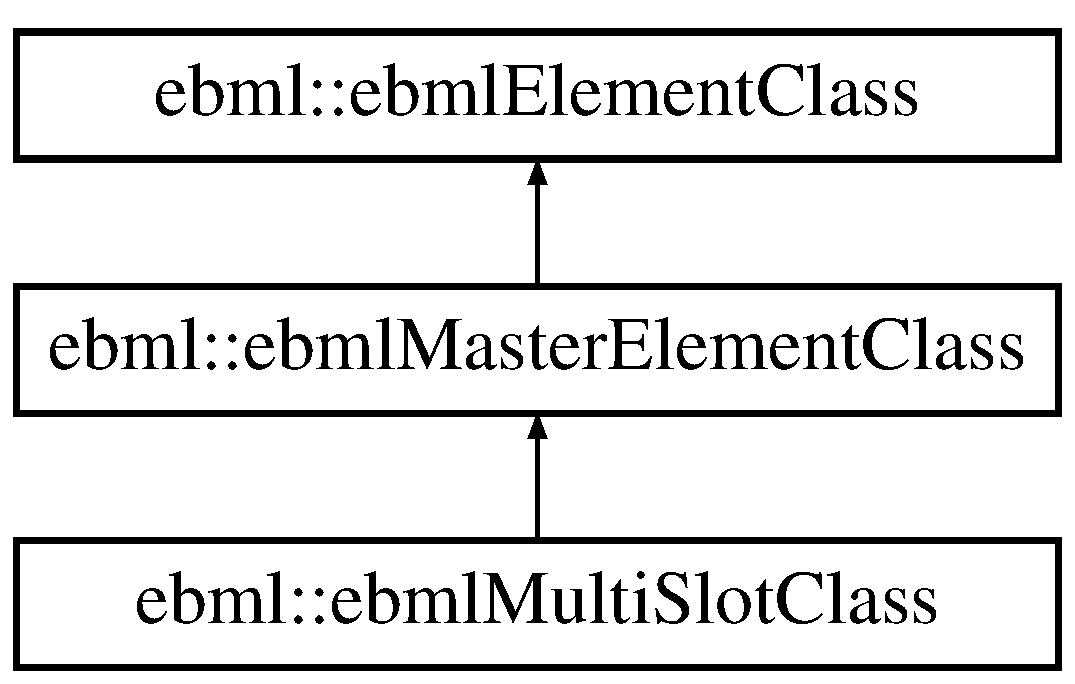
\includegraphics[height=3.000000cm]{classebml_1_1ebmlMultiSlotClass}
\end{center}
\end{figure}
\subsection*{Public Member Functions}
\begin{DoxyCompactItemize}
\item 
\mbox{\hyperlink{classebml_1_1ebmlMultiSlotClass_ac21125f15a5af98e4aa6e8ce494c8667}{ebml\+Multi\+Slot\+Class}} (const char $\ast$, const std\+::wstring \&, const \mbox{\hyperlink{namespaceebml_abdc1248164e4e424423defac9fff7d4d}{slot\+Spec\+\_\+l}} \&)
\item 
\mbox{\hyperlink{classebml_1_1ebmlMultiSlotClass_a455cc78a25f193348d71a2f7f079dd98}{ebml\+Multi\+Slot\+Class}} (const char $\ast$, const std\+::wstring \&, const \mbox{\hyperlink{namespaceebml_abdc1248164e4e424423defac9fff7d4d}{slot\+Spec\+\_\+l}} \&, const \mbox{\hyperlink{structebml_1_1occurSpec__t}{occur\+Spec\+\_\+t}} \&recursive, size\+\_\+t recurseslot)
\item 
\mbox{\hyperlink{classebml_1_1ebmlMultiSlotClass_ac96d2f773a6c8e18731732c97a783fe6}{ebml\+Multi\+Slot\+Class}} (\mbox{\hyperlink{namespaceebml_a86c5f604ddf12a74aa9812e997a58691}{ebml\+I\+D\+\_\+t}}, const std\+::wstring \&, const \mbox{\hyperlink{namespaceebml_abdc1248164e4e424423defac9fff7d4d}{slot\+Spec\+\_\+l}} \&)
\item 
\mbox{\hyperlink{classebml_1_1ebmlMultiSlotClass_ac657dd7c6bd7a89928df88babbff9009}{ebml\+Multi\+Slot\+Class}} (\mbox{\hyperlink{namespaceebml_a86c5f604ddf12a74aa9812e997a58691}{ebml\+I\+D\+\_\+t}}, const std\+::wstring \&, const \mbox{\hyperlink{namespaceebml_abdc1248164e4e424423defac9fff7d4d}{slot\+Spec\+\_\+l}} \&, const \mbox{\hyperlink{structebml_1_1occurSpec__t}{occur\+Spec\+\_\+t}} \&recursive, size\+\_\+t recurseslot)
\item 
\mbox{\hyperlink{namespaceebml_adad533b7705a16bb360fe56380c5e7be}{ebml\+Element\+\_\+sp}} \mbox{\hyperlink{classebml_1_1ebmlMultiSlotClass_a96e8fd5660f5802d19f140b0dc0d042a}{operator()}} (const \mbox{\hyperlink{namespaceebml_ae432575dfbb3e141ce897442794f0ca5}{slot\+Arg\+\_\+l}} \&) const
\item 
\mbox{\hyperlink{namespaceebml_adad533b7705a16bb360fe56380c5e7be}{ebml\+Element\+\_\+sp}} \mbox{\hyperlink{classebml_1_1ebmlMultiSlotClass_a2a4b742e61f4efc0b8e9e686908424d2}{operator()}} (const \mbox{\hyperlink{namespaceebml_a4317d4c495715eced3ed448c2d05caeb}{slot\+Arg\+\_\+d}} \&) const
\item 
\mbox{\hyperlink{namespaceebml_adad533b7705a16bb360fe56380c5e7be}{ebml\+Element\+\_\+sp}} \mbox{\hyperlink{classebml_1_1ebmlMultiSlotClass_a6eaf23b998e3b91075f824842e746bbf}{operator()}} (const \mbox{\hyperlink{namespaceebml_ae432575dfbb3e141ce897442794f0ca5}{slot\+Arg\+\_\+l}} \&, const \mbox{\hyperlink{namespaceebml_a4317d4c495715eced3ed448c2d05caeb}{slot\+Arg\+\_\+d}} \&) const
\item 
\mbox{\hyperlink{namespaceebml_adad533b7705a16bb360fe56380c5e7be}{ebml\+Element\+\_\+sp}} \mbox{\hyperlink{classebml_1_1ebmlMultiSlotClass_ae62906b659277cc8de283a27a8bceed2}{operator()}} (\mbox{\hyperlink{namespaceebml_ae432575dfbb3e141ce897442794f0ca5}{slot\+Arg\+\_\+l}} \&\&) const
\item 
\mbox{\hyperlink{namespaceebml_adad533b7705a16bb360fe56380c5e7be}{ebml\+Element\+\_\+sp}} \mbox{\hyperlink{classebml_1_1ebmlMultiSlotClass_aaba4e03050493237191b214950972295}{operator()}} (\mbox{\hyperlink{namespaceebml_a4317d4c495715eced3ed448c2d05caeb}{slot\+Arg\+\_\+d}} \&\&) const
\item 
\mbox{\hyperlink{namespaceebml_adad533b7705a16bb360fe56380c5e7be}{ebml\+Element\+\_\+sp}} \mbox{\hyperlink{classebml_1_1ebmlMultiSlotClass_a22f33854de534b0cee9c7e2fe8d3be00}{operator()}} (\mbox{\hyperlink{namespaceebml_ae432575dfbb3e141ce897442794f0ca5}{slot\+Arg\+\_\+l}} \&\&, \mbox{\hyperlink{namespaceebml_a4317d4c495715eced3ed448c2d05caeb}{slot\+Arg\+\_\+d}} \&\&) const
\item 
const std\+::vector$<$ \mbox{\hyperlink{classebml_1_1slotSpec__t}{slot\+Spec\+\_\+t}} $>$ \& \mbox{\hyperlink{classebml_1_1ebmlMultiSlotClass_a8c0a510fb0de82566caa77d27127937c}{slot\+Specs}} () const
\item 
const std\+::unordered\+\_\+map$<$ std\+::string, const \mbox{\hyperlink{classebml_1_1slotSpec__t}{slot\+Spec\+\_\+t}} $\ast$ $>$ \& \mbox{\hyperlink{classebml_1_1ebmlMultiSlotClass_a57c1d13ad108cdd5b0cb0b717ef4ef92}{slot\+Specs\+By\+Key}} () const
\item 
const std\+::unordered\+\_\+map$<$ \mbox{\hyperlink{namespaceebml_a86c5f604ddf12a74aa9812e997a58691}{ebml\+I\+D\+\_\+t}}, const \mbox{\hyperlink{classebml_1_1slotSpec__t}{slot\+Spec\+\_\+t}} $\ast$ $>$ \& \mbox{\hyperlink{classebml_1_1ebmlMultiSlotClass_abb2d4a01a3c8048471cc26d5f14dc88d}{slot\+Specs\+By\+ID}} () const
\end{DoxyCompactItemize}
\subsection*{Protected Member Functions}
\begin{DoxyCompactItemize}
\item 
\mbox{\hyperlink{classebml_1_1ebmlElement}{ebml\+Element}} $\ast$ \mbox{\hyperlink{classebml_1_1ebmlMultiSlotClass_ab0cb2ed53ef6a3a8e64ffc47c72f5b94}{\+\_\+new}} () const override
\end{DoxyCompactItemize}
\subsection*{Friends}
\begin{DoxyCompactItemize}
\item 
class \mbox{\hyperlink{classebml_1_1ebmlMultiSlotClass_ab14eb6c5a125d7276a7b4b5b6573428b}{ebml\+Multi\+Slot}}
\end{DoxyCompactItemize}
\subsection*{Additional Inherited Members}


\subsection{Constructor \& Destructor Documentation}
\mbox{\Hypertarget{classebml_1_1ebmlMultiSlotClass_ac21125f15a5af98e4aa6e8ce494c8667}\label{classebml_1_1ebmlMultiSlotClass_ac21125f15a5af98e4aa6e8ce494c8667}} 
\index{ebml\+::ebml\+Multi\+Slot\+Class@{ebml\+::ebml\+Multi\+Slot\+Class}!ebml\+Multi\+Slot\+Class@{ebml\+Multi\+Slot\+Class}}
\index{ebml\+Multi\+Slot\+Class@{ebml\+Multi\+Slot\+Class}!ebml\+::ebml\+Multi\+Slot\+Class@{ebml\+::ebml\+Multi\+Slot\+Class}}
\subsubsection{\texorpdfstring{ebml\+Multi\+Slot\+Class()}{ebmlMultiSlotClass()}\hspace{0.1cm}{\footnotesize\ttfamily [1/4]}}
{\footnotesize\ttfamily ebml\+::ebml\+Multi\+Slot\+Class\+::ebml\+Multi\+Slot\+Class (\begin{DoxyParamCaption}\item[{const char $\ast$}]{,  }\item[{const std\+::wstring \&}]{,  }\item[{const \mbox{\hyperlink{namespaceebml_abdc1248164e4e424423defac9fff7d4d}{slot\+Spec\+\_\+l}} \&}]{ }\end{DoxyParamCaption})}

\mbox{\Hypertarget{classebml_1_1ebmlMultiSlotClass_a455cc78a25f193348d71a2f7f079dd98}\label{classebml_1_1ebmlMultiSlotClass_a455cc78a25f193348d71a2f7f079dd98}} 
\index{ebml\+::ebml\+Multi\+Slot\+Class@{ebml\+::ebml\+Multi\+Slot\+Class}!ebml\+Multi\+Slot\+Class@{ebml\+Multi\+Slot\+Class}}
\index{ebml\+Multi\+Slot\+Class@{ebml\+Multi\+Slot\+Class}!ebml\+::ebml\+Multi\+Slot\+Class@{ebml\+::ebml\+Multi\+Slot\+Class}}
\subsubsection{\texorpdfstring{ebml\+Multi\+Slot\+Class()}{ebmlMultiSlotClass()}\hspace{0.1cm}{\footnotesize\ttfamily [2/4]}}
{\footnotesize\ttfamily ebml\+::ebml\+Multi\+Slot\+Class\+::ebml\+Multi\+Slot\+Class (\begin{DoxyParamCaption}\item[{const char $\ast$}]{,  }\item[{const std\+::wstring \&}]{,  }\item[{const \mbox{\hyperlink{namespaceebml_abdc1248164e4e424423defac9fff7d4d}{slot\+Spec\+\_\+l}} \&}]{,  }\item[{const \mbox{\hyperlink{structebml_1_1occurSpec__t}{occur\+Spec\+\_\+t}} \&}]{recursive,  }\item[{size\+\_\+t}]{recurseslot }\end{DoxyParamCaption})}

\mbox{\Hypertarget{classebml_1_1ebmlMultiSlotClass_ac96d2f773a6c8e18731732c97a783fe6}\label{classebml_1_1ebmlMultiSlotClass_ac96d2f773a6c8e18731732c97a783fe6}} 
\index{ebml\+::ebml\+Multi\+Slot\+Class@{ebml\+::ebml\+Multi\+Slot\+Class}!ebml\+Multi\+Slot\+Class@{ebml\+Multi\+Slot\+Class}}
\index{ebml\+Multi\+Slot\+Class@{ebml\+Multi\+Slot\+Class}!ebml\+::ebml\+Multi\+Slot\+Class@{ebml\+::ebml\+Multi\+Slot\+Class}}
\subsubsection{\texorpdfstring{ebml\+Multi\+Slot\+Class()}{ebmlMultiSlotClass()}\hspace{0.1cm}{\footnotesize\ttfamily [3/4]}}
{\footnotesize\ttfamily ebml\+::ebml\+Multi\+Slot\+Class\+::ebml\+Multi\+Slot\+Class (\begin{DoxyParamCaption}\item[{\mbox{\hyperlink{namespaceebml_a86c5f604ddf12a74aa9812e997a58691}{ebml\+I\+D\+\_\+t}}}]{,  }\item[{const std\+::wstring \&}]{,  }\item[{const \mbox{\hyperlink{namespaceebml_abdc1248164e4e424423defac9fff7d4d}{slot\+Spec\+\_\+l}} \&}]{ }\end{DoxyParamCaption})}

\mbox{\Hypertarget{classebml_1_1ebmlMultiSlotClass_ac657dd7c6bd7a89928df88babbff9009}\label{classebml_1_1ebmlMultiSlotClass_ac657dd7c6bd7a89928df88babbff9009}} 
\index{ebml\+::ebml\+Multi\+Slot\+Class@{ebml\+::ebml\+Multi\+Slot\+Class}!ebml\+Multi\+Slot\+Class@{ebml\+Multi\+Slot\+Class}}
\index{ebml\+Multi\+Slot\+Class@{ebml\+Multi\+Slot\+Class}!ebml\+::ebml\+Multi\+Slot\+Class@{ebml\+::ebml\+Multi\+Slot\+Class}}
\subsubsection{\texorpdfstring{ebml\+Multi\+Slot\+Class()}{ebmlMultiSlotClass()}\hspace{0.1cm}{\footnotesize\ttfamily [4/4]}}
{\footnotesize\ttfamily ebml\+::ebml\+Multi\+Slot\+Class\+::ebml\+Multi\+Slot\+Class (\begin{DoxyParamCaption}\item[{\mbox{\hyperlink{namespaceebml_a86c5f604ddf12a74aa9812e997a58691}{ebml\+I\+D\+\_\+t}}}]{,  }\item[{const std\+::wstring \&}]{,  }\item[{const \mbox{\hyperlink{namespaceebml_abdc1248164e4e424423defac9fff7d4d}{slot\+Spec\+\_\+l}} \&}]{,  }\item[{const \mbox{\hyperlink{structebml_1_1occurSpec__t}{occur\+Spec\+\_\+t}} \&}]{recursive,  }\item[{size\+\_\+t}]{recurseslot }\end{DoxyParamCaption})}



\subsection{Member Function Documentation}
\mbox{\Hypertarget{classebml_1_1ebmlMultiSlotClass_ab0cb2ed53ef6a3a8e64ffc47c72f5b94}\label{classebml_1_1ebmlMultiSlotClass_ab0cb2ed53ef6a3a8e64ffc47c72f5b94}} 
\index{ebml\+::ebml\+Multi\+Slot\+Class@{ebml\+::ebml\+Multi\+Slot\+Class}!\+\_\+new@{\+\_\+new}}
\index{\+\_\+new@{\+\_\+new}!ebml\+::ebml\+Multi\+Slot\+Class@{ebml\+::ebml\+Multi\+Slot\+Class}}
\subsubsection{\texorpdfstring{\+\_\+new()}{\_new()}}
{\footnotesize\ttfamily \mbox{\hyperlink{classebml_1_1ebmlElement}{ebml\+Element}}$\ast$ ebml\+::ebml\+Multi\+Slot\+Class\+::\+\_\+new (\begin{DoxyParamCaption}{ }\end{DoxyParamCaption}) const\hspace{0.3cm}{\ttfamily [override]}, {\ttfamily [protected]}, {\ttfamily [virtual]}}



Implements \mbox{\hyperlink{classebml_1_1ebmlElementClass_a223ede6b8bc3c85251d2d73f0256fb45}{ebml\+::ebml\+Element\+Class}}.

\mbox{\Hypertarget{classebml_1_1ebmlMultiSlotClass_a96e8fd5660f5802d19f140b0dc0d042a}\label{classebml_1_1ebmlMultiSlotClass_a96e8fd5660f5802d19f140b0dc0d042a}} 
\index{ebml\+::ebml\+Multi\+Slot\+Class@{ebml\+::ebml\+Multi\+Slot\+Class}!operator()@{operator()}}
\index{operator()@{operator()}!ebml\+::ebml\+Multi\+Slot\+Class@{ebml\+::ebml\+Multi\+Slot\+Class}}
\subsubsection{\texorpdfstring{operator()()}{operator()()}\hspace{0.1cm}{\footnotesize\ttfamily [1/6]}}
{\footnotesize\ttfamily \mbox{\hyperlink{namespaceebml_adad533b7705a16bb360fe56380c5e7be}{ebml\+Element\+\_\+sp}} ebml\+::ebml\+Multi\+Slot\+Class\+::operator() (\begin{DoxyParamCaption}\item[{const \mbox{\hyperlink{namespaceebml_ae432575dfbb3e141ce897442794f0ca5}{slot\+Arg\+\_\+l}} \&}]{ }\end{DoxyParamCaption}) const}

\mbox{\Hypertarget{classebml_1_1ebmlMultiSlotClass_a2a4b742e61f4efc0b8e9e686908424d2}\label{classebml_1_1ebmlMultiSlotClass_a2a4b742e61f4efc0b8e9e686908424d2}} 
\index{ebml\+::ebml\+Multi\+Slot\+Class@{ebml\+::ebml\+Multi\+Slot\+Class}!operator()@{operator()}}
\index{operator()@{operator()}!ebml\+::ebml\+Multi\+Slot\+Class@{ebml\+::ebml\+Multi\+Slot\+Class}}
\subsubsection{\texorpdfstring{operator()()}{operator()()}\hspace{0.1cm}{\footnotesize\ttfamily [2/6]}}
{\footnotesize\ttfamily \mbox{\hyperlink{namespaceebml_adad533b7705a16bb360fe56380c5e7be}{ebml\+Element\+\_\+sp}} ebml\+::ebml\+Multi\+Slot\+Class\+::operator() (\begin{DoxyParamCaption}\item[{const \mbox{\hyperlink{namespaceebml_a4317d4c495715eced3ed448c2d05caeb}{slot\+Arg\+\_\+d}} \&}]{ }\end{DoxyParamCaption}) const}

\mbox{\Hypertarget{classebml_1_1ebmlMultiSlotClass_a6eaf23b998e3b91075f824842e746bbf}\label{classebml_1_1ebmlMultiSlotClass_a6eaf23b998e3b91075f824842e746bbf}} 
\index{ebml\+::ebml\+Multi\+Slot\+Class@{ebml\+::ebml\+Multi\+Slot\+Class}!operator()@{operator()}}
\index{operator()@{operator()}!ebml\+::ebml\+Multi\+Slot\+Class@{ebml\+::ebml\+Multi\+Slot\+Class}}
\subsubsection{\texorpdfstring{operator()()}{operator()()}\hspace{0.1cm}{\footnotesize\ttfamily [3/6]}}
{\footnotesize\ttfamily \mbox{\hyperlink{namespaceebml_adad533b7705a16bb360fe56380c5e7be}{ebml\+Element\+\_\+sp}} ebml\+::ebml\+Multi\+Slot\+Class\+::operator() (\begin{DoxyParamCaption}\item[{const \mbox{\hyperlink{namespaceebml_ae432575dfbb3e141ce897442794f0ca5}{slot\+Arg\+\_\+l}} \&}]{,  }\item[{const \mbox{\hyperlink{namespaceebml_a4317d4c495715eced3ed448c2d05caeb}{slot\+Arg\+\_\+d}} \&}]{ }\end{DoxyParamCaption}) const}

\mbox{\Hypertarget{classebml_1_1ebmlMultiSlotClass_ae62906b659277cc8de283a27a8bceed2}\label{classebml_1_1ebmlMultiSlotClass_ae62906b659277cc8de283a27a8bceed2}} 
\index{ebml\+::ebml\+Multi\+Slot\+Class@{ebml\+::ebml\+Multi\+Slot\+Class}!operator()@{operator()}}
\index{operator()@{operator()}!ebml\+::ebml\+Multi\+Slot\+Class@{ebml\+::ebml\+Multi\+Slot\+Class}}
\subsubsection{\texorpdfstring{operator()()}{operator()()}\hspace{0.1cm}{\footnotesize\ttfamily [4/6]}}
{\footnotesize\ttfamily \mbox{\hyperlink{namespaceebml_adad533b7705a16bb360fe56380c5e7be}{ebml\+Element\+\_\+sp}} ebml\+::ebml\+Multi\+Slot\+Class\+::operator() (\begin{DoxyParamCaption}\item[{\mbox{\hyperlink{namespaceebml_ae432575dfbb3e141ce897442794f0ca5}{slot\+Arg\+\_\+l}} \&\&}]{ }\end{DoxyParamCaption}) const}

\mbox{\Hypertarget{classebml_1_1ebmlMultiSlotClass_aaba4e03050493237191b214950972295}\label{classebml_1_1ebmlMultiSlotClass_aaba4e03050493237191b214950972295}} 
\index{ebml\+::ebml\+Multi\+Slot\+Class@{ebml\+::ebml\+Multi\+Slot\+Class}!operator()@{operator()}}
\index{operator()@{operator()}!ebml\+::ebml\+Multi\+Slot\+Class@{ebml\+::ebml\+Multi\+Slot\+Class}}
\subsubsection{\texorpdfstring{operator()()}{operator()()}\hspace{0.1cm}{\footnotesize\ttfamily [5/6]}}
{\footnotesize\ttfamily \mbox{\hyperlink{namespaceebml_adad533b7705a16bb360fe56380c5e7be}{ebml\+Element\+\_\+sp}} ebml\+::ebml\+Multi\+Slot\+Class\+::operator() (\begin{DoxyParamCaption}\item[{\mbox{\hyperlink{namespaceebml_a4317d4c495715eced3ed448c2d05caeb}{slot\+Arg\+\_\+d}} \&\&}]{ }\end{DoxyParamCaption}) const}

\mbox{\Hypertarget{classebml_1_1ebmlMultiSlotClass_a22f33854de534b0cee9c7e2fe8d3be00}\label{classebml_1_1ebmlMultiSlotClass_a22f33854de534b0cee9c7e2fe8d3be00}} 
\index{ebml\+::ebml\+Multi\+Slot\+Class@{ebml\+::ebml\+Multi\+Slot\+Class}!operator()@{operator()}}
\index{operator()@{operator()}!ebml\+::ebml\+Multi\+Slot\+Class@{ebml\+::ebml\+Multi\+Slot\+Class}}
\subsubsection{\texorpdfstring{operator()()}{operator()()}\hspace{0.1cm}{\footnotesize\ttfamily [6/6]}}
{\footnotesize\ttfamily \mbox{\hyperlink{namespaceebml_adad533b7705a16bb360fe56380c5e7be}{ebml\+Element\+\_\+sp}} ebml\+::ebml\+Multi\+Slot\+Class\+::operator() (\begin{DoxyParamCaption}\item[{\mbox{\hyperlink{namespaceebml_ae432575dfbb3e141ce897442794f0ca5}{slot\+Arg\+\_\+l}} \&\&}]{,  }\item[{\mbox{\hyperlink{namespaceebml_a4317d4c495715eced3ed448c2d05caeb}{slot\+Arg\+\_\+d}} \&\&}]{ }\end{DoxyParamCaption}) const}

\mbox{\Hypertarget{classebml_1_1ebmlMultiSlotClass_a8c0a510fb0de82566caa77d27127937c}\label{classebml_1_1ebmlMultiSlotClass_a8c0a510fb0de82566caa77d27127937c}} 
\index{ebml\+::ebml\+Multi\+Slot\+Class@{ebml\+::ebml\+Multi\+Slot\+Class}!slot\+Specs@{slot\+Specs}}
\index{slot\+Specs@{slot\+Specs}!ebml\+::ebml\+Multi\+Slot\+Class@{ebml\+::ebml\+Multi\+Slot\+Class}}
\subsubsection{\texorpdfstring{slot\+Specs()}{slotSpecs()}}
{\footnotesize\ttfamily const std\+::vector$<$\mbox{\hyperlink{classebml_1_1slotSpec__t}{slot\+Spec\+\_\+t}}$>$\& ebml\+::ebml\+Multi\+Slot\+Class\+::slot\+Specs (\begin{DoxyParamCaption}{ }\end{DoxyParamCaption}) const}

\mbox{\Hypertarget{classebml_1_1ebmlMultiSlotClass_abb2d4a01a3c8048471cc26d5f14dc88d}\label{classebml_1_1ebmlMultiSlotClass_abb2d4a01a3c8048471cc26d5f14dc88d}} 
\index{ebml\+::ebml\+Multi\+Slot\+Class@{ebml\+::ebml\+Multi\+Slot\+Class}!slot\+Specs\+By\+ID@{slot\+Specs\+By\+ID}}
\index{slot\+Specs\+By\+ID@{slot\+Specs\+By\+ID}!ebml\+::ebml\+Multi\+Slot\+Class@{ebml\+::ebml\+Multi\+Slot\+Class}}
\subsubsection{\texorpdfstring{slot\+Specs\+By\+I\+D()}{slotSpecsByID()}}
{\footnotesize\ttfamily const std\+::unordered\+\_\+map$<$\mbox{\hyperlink{namespaceebml_a86c5f604ddf12a74aa9812e997a58691}{ebml\+I\+D\+\_\+t}}, const \mbox{\hyperlink{classebml_1_1slotSpec__t}{slot\+Spec\+\_\+t}}$\ast$$>$\& ebml\+::ebml\+Multi\+Slot\+Class\+::slot\+Specs\+By\+ID (\begin{DoxyParamCaption}{ }\end{DoxyParamCaption}) const}

\mbox{\Hypertarget{classebml_1_1ebmlMultiSlotClass_a57c1d13ad108cdd5b0cb0b717ef4ef92}\label{classebml_1_1ebmlMultiSlotClass_a57c1d13ad108cdd5b0cb0b717ef4ef92}} 
\index{ebml\+::ebml\+Multi\+Slot\+Class@{ebml\+::ebml\+Multi\+Slot\+Class}!slot\+Specs\+By\+Key@{slot\+Specs\+By\+Key}}
\index{slot\+Specs\+By\+Key@{slot\+Specs\+By\+Key}!ebml\+::ebml\+Multi\+Slot\+Class@{ebml\+::ebml\+Multi\+Slot\+Class}}
\subsubsection{\texorpdfstring{slot\+Specs\+By\+Key()}{slotSpecsByKey()}}
{\footnotesize\ttfamily const std\+::unordered\+\_\+map$<$std\+::string, const \mbox{\hyperlink{classebml_1_1slotSpec__t}{slot\+Spec\+\_\+t}}$\ast$$>$\& ebml\+::ebml\+Multi\+Slot\+Class\+::slot\+Specs\+By\+Key (\begin{DoxyParamCaption}{ }\end{DoxyParamCaption}) const}



\subsection{Friends And Related Function Documentation}
\mbox{\Hypertarget{classebml_1_1ebmlMultiSlotClass_ab14eb6c5a125d7276a7b4b5b6573428b}\label{classebml_1_1ebmlMultiSlotClass_ab14eb6c5a125d7276a7b4b5b6573428b}} 
\index{ebml\+::ebml\+Multi\+Slot\+Class@{ebml\+::ebml\+Multi\+Slot\+Class}!ebml\+Multi\+Slot@{ebml\+Multi\+Slot}}
\index{ebml\+Multi\+Slot@{ebml\+Multi\+Slot}!ebml\+::ebml\+Multi\+Slot\+Class@{ebml\+::ebml\+Multi\+Slot\+Class}}
\subsubsection{\texorpdfstring{ebml\+Multi\+Slot}{ebmlMultiSlot}}
{\footnotesize\ttfamily friend class \mbox{\hyperlink{classebml_1_1ebmlMultiSlot}{ebml\+Multi\+Slot}}\hspace{0.3cm}{\ttfamily [friend]}}



The documentation for this class was generated from the following file\+:\begin{DoxyCompactItemize}
\item 
include/libebml\+\_\+ng/masterelement/\mbox{\hyperlink{multislot_8h}{multislot.\+h}}\end{DoxyCompactItemize}

\hypertarget{classebml_1_1ebmlNoChildMatch}{}\section{ebml\+:\+:ebml\+No\+Child\+Match Class Reference}
\label{classebml_1_1ebmlNoChildMatch}\index{ebml\+::ebml\+No\+Child\+Match@{ebml\+::ebml\+No\+Child\+Match}}


{\ttfamily \#include $<$exceptions.\+h$>$}

Inheritance diagram for ebml\+:\+:ebml\+No\+Child\+Match\+:\begin{figure}[H]
\begin{center}
\leavevmode
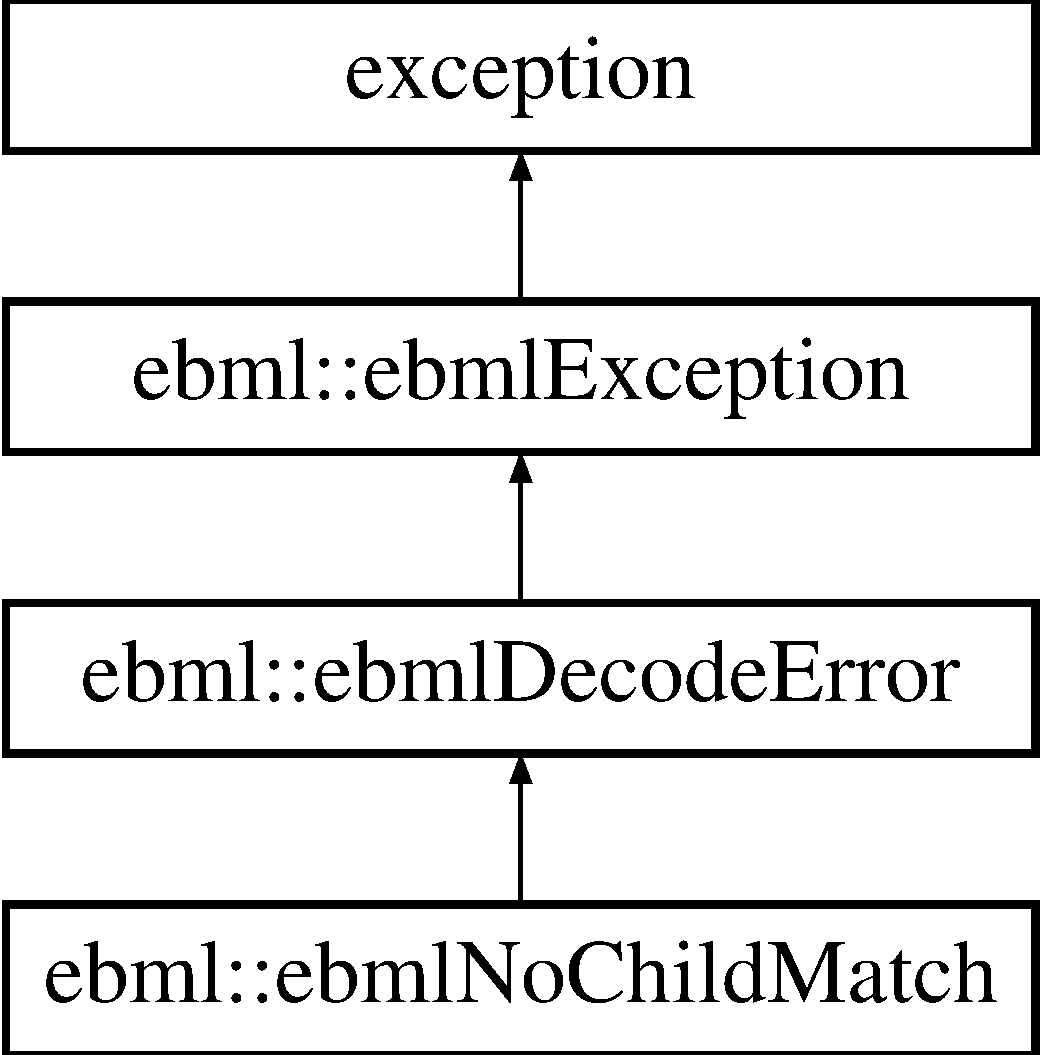
\includegraphics[height=4.000000cm]{classebml_1_1ebmlNoChildMatch}
\end{center}
\end{figure}
\subsection*{Public Member Functions}
\begin{DoxyCompactItemize}
\item 
\mbox{\hyperlink{classebml_1_1ebmlNoChildMatch_aa4f5e655f9247308a8d066c06f213a7e}{ebml\+No\+Child\+Match}} (const std\+::string \&message, const \mbox{\hyperlink{classebml_1_1ebmlElementClass}{ebml\+Element\+Class}} $\ast$\mbox{\hyperlink{classebml_1_1ebmlDecodeError_a3568b4ea3cd5bd16b9510abfe269920f}{cls}}=nullptr, off\+\_\+t \mbox{\hyperlink{classebml_1_1ebmlDecodeError_ad32ac9b3dd52f1c11479085d9c665e0f}{offset}}=-\/1, unsigned char \mbox{\hyperlink{classebml_1_1ebmlDecodeError_a61a4d4856f0c779a1c216e45dc5a7c1e}{head\+Size}}=0, off\+\_\+t \mbox{\hyperlink{classebml_1_1ebmlDecodeError_acb525117e0109d9640fb5e8c546e9a02}{erroroffset}}=-\/1)
\end{DoxyCompactItemize}
\subsection*{Additional Inherited Members}


\subsection{Constructor \& Destructor Documentation}
\mbox{\Hypertarget{classebml_1_1ebmlNoChildMatch_aa4f5e655f9247308a8d066c06f213a7e}\label{classebml_1_1ebmlNoChildMatch_aa4f5e655f9247308a8d066c06f213a7e}} 
\index{ebml\+::ebml\+No\+Child\+Match@{ebml\+::ebml\+No\+Child\+Match}!ebml\+No\+Child\+Match@{ebml\+No\+Child\+Match}}
\index{ebml\+No\+Child\+Match@{ebml\+No\+Child\+Match}!ebml\+::ebml\+No\+Child\+Match@{ebml\+::ebml\+No\+Child\+Match}}
\subsubsection{\texorpdfstring{ebml\+No\+Child\+Match()}{ebmlNoChildMatch()}}
{\footnotesize\ttfamily ebml\+::ebml\+No\+Child\+Match\+::ebml\+No\+Child\+Match (\begin{DoxyParamCaption}\item[{const std\+::string \&}]{message,  }\item[{const \mbox{\hyperlink{classebml_1_1ebmlElementClass}{ebml\+Element\+Class}} $\ast$}]{cls = {\ttfamily nullptr},  }\item[{off\+\_\+t}]{offset = {\ttfamily -\/1},  }\item[{unsigned char}]{head\+Size = {\ttfamily 0},  }\item[{off\+\_\+t}]{erroroffset = {\ttfamily -\/1} }\end{DoxyParamCaption})}



The documentation for this class was generated from the following file\+:\begin{DoxyCompactItemize}
\item 
include/libebml\+\_\+ng/\mbox{\hyperlink{exceptions_8h}{exceptions.\+h}}\end{DoxyCompactItemize}

\hypertarget{classebml_1_1ebmlNoMatch}{}\section{ebml\+:\+:ebml\+No\+Match Class Reference}
\label{classebml_1_1ebmlNoMatch}\index{ebml\+::ebml\+No\+Match@{ebml\+::ebml\+No\+Match}}


{\ttfamily \#include $<$exceptions.\+h$>$}

Inheritance diagram for ebml\+:\+:ebml\+No\+Match\+:\begin{figure}[H]
\begin{center}
\leavevmode
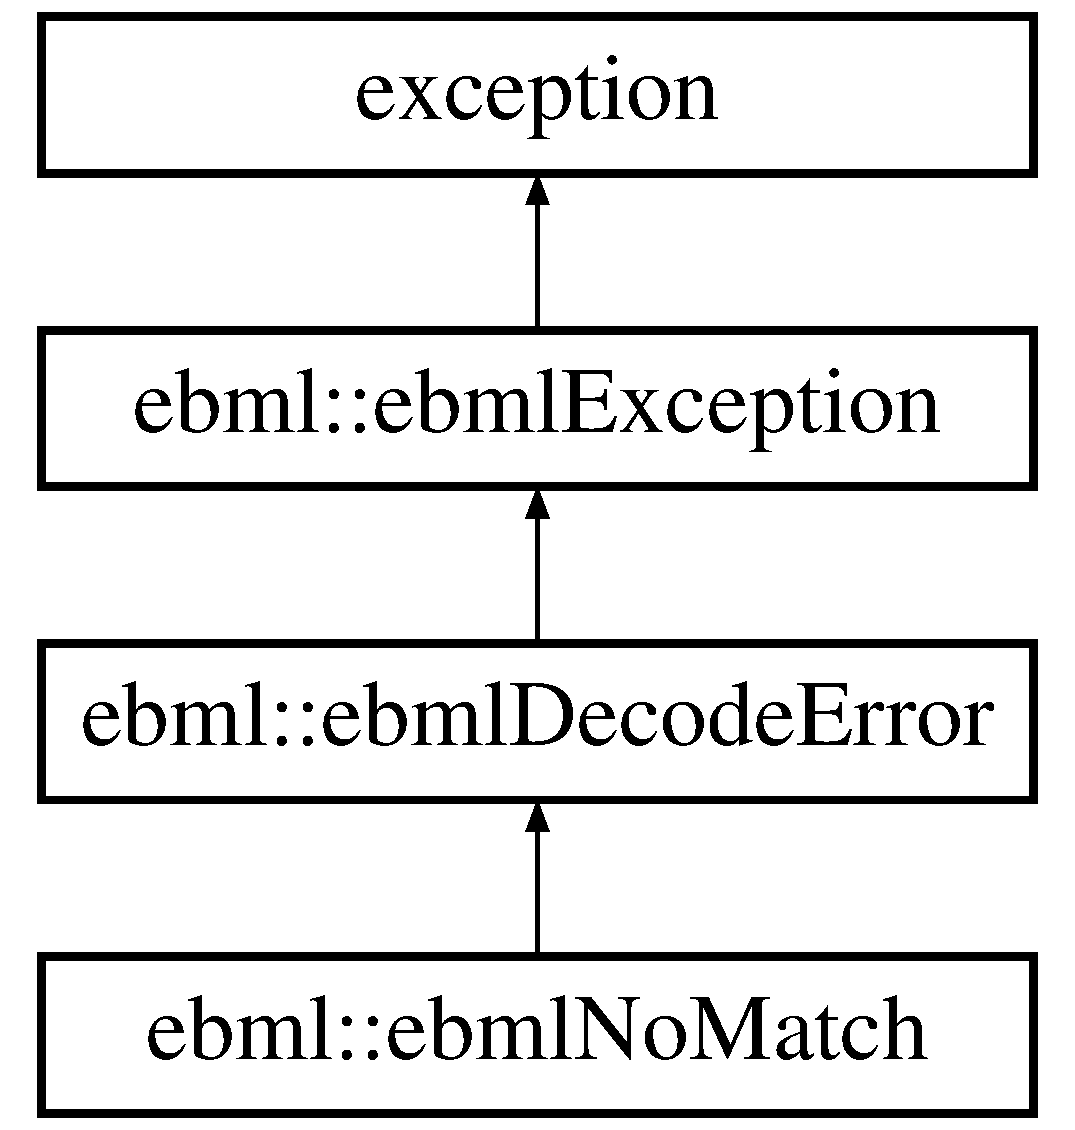
\includegraphics[height=4.000000cm]{classebml_1_1ebmlNoMatch}
\end{center}
\end{figure}
\subsection*{Public Member Functions}
\begin{DoxyCompactItemize}
\item 
\mbox{\hyperlink{classebml_1_1ebmlNoMatch_aa17ff365ad72c2d723582442dd2295b8}{ebml\+No\+Match}} (const std\+::string \&message, const \mbox{\hyperlink{classebml_1_1ebmlElementClass}{ebml\+Element\+Class}} $\ast$\mbox{\hyperlink{classebml_1_1ebmlDecodeError_a3568b4ea3cd5bd16b9510abfe269920f}{cls}}=nullptr, off\+\_\+t \mbox{\hyperlink{classebml_1_1ebmlDecodeError_ad32ac9b3dd52f1c11479085d9c665e0f}{offset}}=-\/1, unsigned char \mbox{\hyperlink{classebml_1_1ebmlDecodeError_a61a4d4856f0c779a1c216e45dc5a7c1e}{head\+Size}}=0, off\+\_\+t \mbox{\hyperlink{classebml_1_1ebmlDecodeError_acb525117e0109d9640fb5e8c546e9a02}{erroroffset}}=-\/1)
\end{DoxyCompactItemize}
\subsection*{Additional Inherited Members}


\subsection{Constructor \& Destructor Documentation}
\mbox{\Hypertarget{classebml_1_1ebmlNoMatch_aa17ff365ad72c2d723582442dd2295b8}\label{classebml_1_1ebmlNoMatch_aa17ff365ad72c2d723582442dd2295b8}} 
\index{ebml\+::ebml\+No\+Match@{ebml\+::ebml\+No\+Match}!ebml\+No\+Match@{ebml\+No\+Match}}
\index{ebml\+No\+Match@{ebml\+No\+Match}!ebml\+::ebml\+No\+Match@{ebml\+::ebml\+No\+Match}}
\subsubsection{\texorpdfstring{ebml\+No\+Match()}{ebmlNoMatch()}}
{\footnotesize\ttfamily ebml\+::ebml\+No\+Match\+::ebml\+No\+Match (\begin{DoxyParamCaption}\item[{const std\+::string \&}]{message,  }\item[{const \mbox{\hyperlink{classebml_1_1ebmlElementClass}{ebml\+Element\+Class}} $\ast$}]{cls = {\ttfamily nullptr},  }\item[{off\+\_\+t}]{offset = {\ttfamily -\/1},  }\item[{unsigned char}]{head\+Size = {\ttfamily 0},  }\item[{off\+\_\+t}]{erroroffset = {\ttfamily -\/1} }\end{DoxyParamCaption})}



The documentation for this class was generated from the following file\+:\begin{DoxyCompactItemize}
\item 
include/libebml\+\_\+ng/\mbox{\hyperlink{exceptions_8h}{exceptions.\+h}}\end{DoxyCompactItemize}

\hypertarget{classebml_1_1ebmlNotImplementedError}{}\section{ebml\+:\+:ebml\+Not\+Implemented\+Error Class Reference}
\label{classebml_1_1ebmlNotImplementedError}\index{ebml\+::ebml\+Not\+Implemented\+Error@{ebml\+::ebml\+Not\+Implemented\+Error}}


{\ttfamily \#include $<$exceptions.\+h$>$}

Inheritance diagram for ebml\+:\+:ebml\+Not\+Implemented\+Error\+:\begin{figure}[H]
\begin{center}
\leavevmode
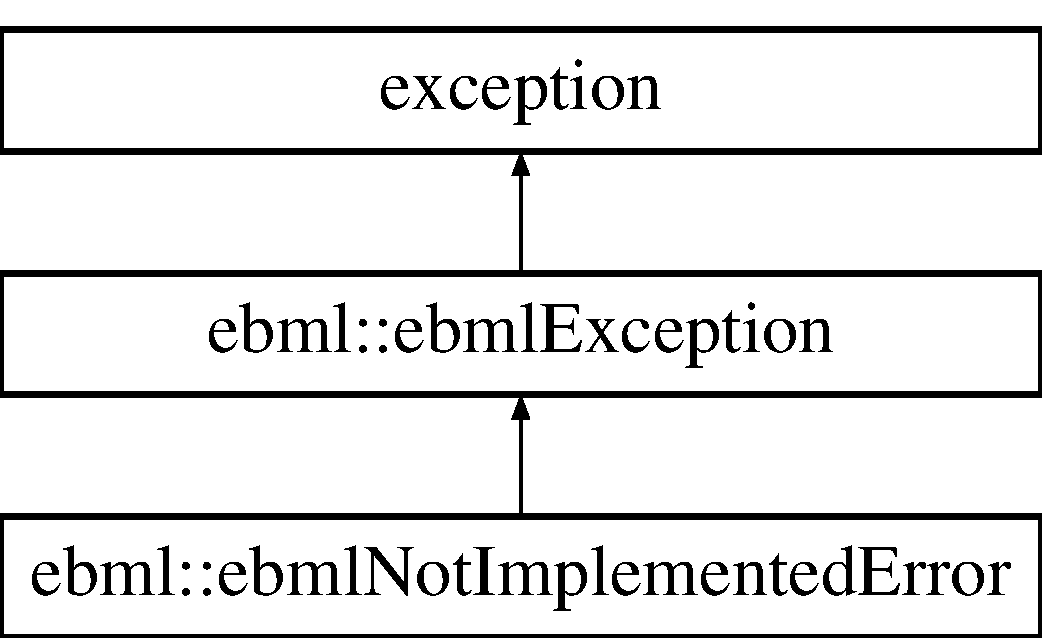
\includegraphics[height=3.000000cm]{classebml_1_1ebmlNotImplementedError}
\end{center}
\end{figure}
\subsection*{Public Member Functions}
\begin{DoxyCompactItemize}
\item 
\mbox{\hyperlink{classebml_1_1ebmlNotImplementedError_aef5d5bfbae1bb89105fc7cf89563e710}{ebml\+Not\+Implemented\+Error}} (const std\+::string \&message, const \mbox{\hyperlink{classebml_1_1ebmlElementClass}{ebml\+Element\+Class}} $\ast$\mbox{\hyperlink{classebml_1_1ebmlNotImplementedError_affef6ae492f6c0ab0c22970955a2e8c9}{cls}}=nullptr)
\end{DoxyCompactItemize}
\subsection*{Public Attributes}
\begin{DoxyCompactItemize}
\item 
const \mbox{\hyperlink{classebml_1_1ebmlElementClass}{ebml\+Element\+Class}} $\ast$ \mbox{\hyperlink{classebml_1_1ebmlNotImplementedError_affef6ae492f6c0ab0c22970955a2e8c9}{cls}}
\end{DoxyCompactItemize}


\subsection{Constructor \& Destructor Documentation}
\mbox{\Hypertarget{classebml_1_1ebmlNotImplementedError_aef5d5bfbae1bb89105fc7cf89563e710}\label{classebml_1_1ebmlNotImplementedError_aef5d5bfbae1bb89105fc7cf89563e710}} 
\index{ebml\+::ebml\+Not\+Implemented\+Error@{ebml\+::ebml\+Not\+Implemented\+Error}!ebml\+Not\+Implemented\+Error@{ebml\+Not\+Implemented\+Error}}
\index{ebml\+Not\+Implemented\+Error@{ebml\+Not\+Implemented\+Error}!ebml\+::ebml\+Not\+Implemented\+Error@{ebml\+::ebml\+Not\+Implemented\+Error}}
\subsubsection{\texorpdfstring{ebml\+Not\+Implemented\+Error()}{ebmlNotImplementedError()}}
{\footnotesize\ttfamily ebml\+::ebml\+Not\+Implemented\+Error\+::ebml\+Not\+Implemented\+Error (\begin{DoxyParamCaption}\item[{const std\+::string \&}]{message,  }\item[{const \mbox{\hyperlink{classebml_1_1ebmlElementClass}{ebml\+Element\+Class}} $\ast$}]{cls = {\ttfamily nullptr} }\end{DoxyParamCaption})}



\subsection{Member Data Documentation}
\mbox{\Hypertarget{classebml_1_1ebmlNotImplementedError_affef6ae492f6c0ab0c22970955a2e8c9}\label{classebml_1_1ebmlNotImplementedError_affef6ae492f6c0ab0c22970955a2e8c9}} 
\index{ebml\+::ebml\+Not\+Implemented\+Error@{ebml\+::ebml\+Not\+Implemented\+Error}!cls@{cls}}
\index{cls@{cls}!ebml\+::ebml\+Not\+Implemented\+Error@{ebml\+::ebml\+Not\+Implemented\+Error}}
\subsubsection{\texorpdfstring{cls}{cls}}
{\footnotesize\ttfamily const \mbox{\hyperlink{classebml_1_1ebmlElementClass}{ebml\+Element\+Class}}$\ast$ ebml\+::ebml\+Not\+Implemented\+Error\+::cls}



The documentation for this class was generated from the following file\+:\begin{DoxyCompactItemize}
\item 
include/libebml\+\_\+ng/\mbox{\hyperlink{exceptions_8h}{exceptions.\+h}}\end{DoxyCompactItemize}

\hypertarget{classebml_1_1ebmlPair}{}\section{ebml\+:\+:ebml\+Pair$<$ T $>$ Class Template Reference}
\label{classebml_1_1ebmlPair}\index{ebml\+::ebml\+Pair$<$ T $>$@{ebml\+::ebml\+Pair$<$ T $>$}}


{\ttfamily \#include $<$map.\+h$>$}

Inheritance diagram for ebml\+:\+:ebml\+Pair$<$ T $>$\+:\begin{figure}[H]
\begin{center}
\leavevmode
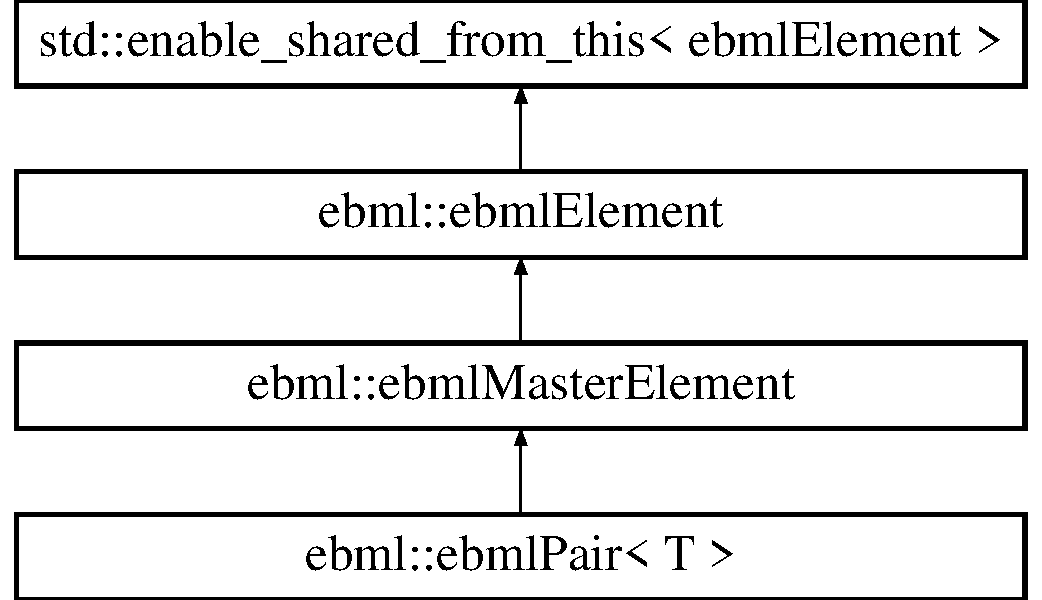
\includegraphics[height=4.000000cm]{classebml_1_1ebmlPair}
\end{center}
\end{figure}
\subsection*{Classes}
\begin{DoxyCompactItemize}
\item 
class \mbox{\hyperlink{classebml_1_1ebmlPair_1_1__const__iterator}{\+\_\+const\+\_\+iterator}}
\item 
class \mbox{\hyperlink{classebml_1_1ebmlPair_1_1__iterator}{\+\_\+iterator}}
\end{DoxyCompactItemize}
\subsection*{Public Member Functions}
\begin{DoxyCompactItemize}
\item 
std\+::wstring \mbox{\hyperlink{classebml_1_1ebmlPair_a88a68eed87260a46f40371f14279da4e}{minirepr}} () const override
\item 
const \mbox{\hyperlink{classebml_1_1ebmlPairClass}{ebml\+Pair\+Class}}$<$ T $>$ $\ast$ \mbox{\hyperlink{classebml_1_1ebmlPair_ad1244458e1390cbf567dfd460b0002f2}{cls}} () const
\item 
T \& \mbox{\hyperlink{classebml_1_1ebmlPair_a0989f9878a29f4c67b801a8744447217}{key}} ()
\item 
const \mbox{\hyperlink{namespaceebml_adad533b7705a16bb360fe56380c5e7be}{ebml\+Element\+\_\+sp}} \& \mbox{\hyperlink{classebml_1_1ebmlPair_a7a68c53d993ced2a13ebe81acce74855}{key\+Elem}} ()
\item 
\mbox{\hyperlink{classebml_1_1childSlot__t}{child\+Slot\+\_\+t}} \mbox{\hyperlink{classebml_1_1ebmlPair_a4808e061fa6ea4b11a7e9490c037bba5}{value}} ()
\item 
const T \& \mbox{\hyperlink{classebml_1_1ebmlPair_a0945a9d73fccd6913c0548c62f08c719}{key}} () const
\item 
\mbox{\hyperlink{namespaceebml_a2deef4e8071531b32e3533f1bf978917}{c\+\_\+ebml\+Element\+\_\+sp}} \mbox{\hyperlink{classebml_1_1ebmlPair_ac9269a9e3f807074b21db614b9f4b2ce}{key\+Elem}} () const
\item 
\mbox{\hyperlink{namespaceebml_a2deef4e8071531b32e3533f1bf978917}{c\+\_\+ebml\+Element\+\_\+sp}} \mbox{\hyperlink{classebml_1_1ebmlPair_abfb141bc1df5ab8c20f0d6d931accb67}{value}} () const
\end{DoxyCompactItemize}
\subsection*{Protected Member Functions}
\begin{DoxyCompactItemize}
\item 
\mbox{\hyperlink{classebml_1_1ebmlPair_a5dadd29820eb5bca6f5bda996f70f06f}{ebml\+Pair}} (const \mbox{\hyperlink{classebml_1_1ebmlPairClass}{ebml\+Pair\+Class}}$<$ T $>$ $\ast$)
\item 
void \mbox{\hyperlink{classebml_1_1ebmlPair_a521c8592475793acf050353ddf56031c}{\+\_\+clear}} () override
\item 
void \mbox{\hyperlink{classebml_1_1ebmlPair_a43ae0c4a471cba5b3c83133951b773ba}{\+\_\+set\+Data}} (const \mbox{\hyperlink{namespaceebml_adad533b7705a16bb360fe56380c5e7be}{ebml\+Element\+\_\+sp}} \&, const \mbox{\hyperlink{namespaceebml_adad533b7705a16bb360fe56380c5e7be}{ebml\+Element\+\_\+sp}} \&)
\item 
void \mbox{\hyperlink{classebml_1_1ebmlPair_af03a41878253632d58c0af0a5121a411}{\+\_\+set\+Data}} (\mbox{\hyperlink{namespaceebml_adad533b7705a16bb360fe56380c5e7be}{ebml\+Element\+\_\+sp}} \&\&, \mbox{\hyperlink{namespaceebml_adad533b7705a16bb360fe56380c5e7be}{ebml\+Element\+\_\+sp}} \&\&)
\item 
void \mbox{\hyperlink{classebml_1_1ebmlPair_a1da4edfcf6f4709e7a33017a3f93dc29}{\+\_\+set\+Data}} (const T \&, const \mbox{\hyperlink{namespaceebml_adad533b7705a16bb360fe56380c5e7be}{ebml\+Element\+\_\+sp}} \&)
\item 
void \mbox{\hyperlink{classebml_1_1ebmlPair_a3cc1fdcae7b1f0b39998735b2802e91e}{\+\_\+set\+Data}} (const T \&, \mbox{\hyperlink{namespaceebml_adad533b7705a16bb360fe56380c5e7be}{ebml\+Element\+\_\+sp}} \&\&)
\item 
void \mbox{\hyperlink{classebml_1_1ebmlPair_acba0d25b5f3882ad2c80bbbb2f135336}{\+\_\+set\+Data}} (T \&\&, \mbox{\hyperlink{namespaceebml_adad533b7705a16bb360fe56380c5e7be}{ebml\+Element\+\_\+sp}} \&\&)
\item 
void \mbox{\hyperlink{classebml_1_1ebmlPair_a6974cf70949c7e2a53754b7fb71d8a72}{\+\_\+set\+Key}} (const \mbox{\hyperlink{namespaceebml_adad533b7705a16bb360fe56380c5e7be}{ebml\+Element\+\_\+sp}} \&)
\item 
void \mbox{\hyperlink{classebml_1_1ebmlPair_a322d953e0ec4e42cb630aa2f1b97dc75}{\+\_\+set\+Key}} (\mbox{\hyperlink{namespaceebml_adad533b7705a16bb360fe56380c5e7be}{ebml\+Element\+\_\+sp}} \&\&)
\item 
void \mbox{\hyperlink{classebml_1_1ebmlPair_ad8a103b58e64c0ae4eb55a4233d41615}{\+\_\+set\+Key}} (const T \&)
\item 
void \mbox{\hyperlink{classebml_1_1ebmlPair_a4eca03083020380229928f80b0226d1b}{\+\_\+set\+Key}} (T \&\&)
\item 
void \mbox{\hyperlink{classebml_1_1ebmlPair_a21a1c612d4032005000b3b4c082b0aa5}{\+\_\+set\+Value}} (const \mbox{\hyperlink{namespaceebml_adad533b7705a16bb360fe56380c5e7be}{ebml\+Element\+\_\+sp}} \&)
\item 
void \mbox{\hyperlink{classebml_1_1ebmlPair_abac0f95caefcfd7b0028cd1f6b70e96d}{\+\_\+set\+Value}} (\mbox{\hyperlink{namespaceebml_adad533b7705a16bb360fe56380c5e7be}{ebml\+Element\+\_\+sp}} \&\&)
\item 
\mbox{\hyperlink{classebml_1_1ebmlMasterElement_1_1__iterator}{ebml\+Master\+Element\+::\+\_\+iterator}} $\ast$ \mbox{\hyperlink{classebml_1_1ebmlPair_a1bd75b88b0b88d39a48283a2d8e9be4e}{\+\_\+begin}} () override
\item 
\mbox{\hyperlink{classebml_1_1ebmlMasterElement_1_1__iterator}{ebml\+Master\+Element\+::\+\_\+iterator}} $\ast$ \mbox{\hyperlink{classebml_1_1ebmlPair_aa9885eed27f8a81efe246b5a6755186b}{\+\_\+end}} () override
\item 
\mbox{\hyperlink{classebml_1_1ebmlMasterElement_1_1__const__iterator}{ebml\+Master\+Element\+::\+\_\+const\+\_\+iterator}} $\ast$ \mbox{\hyperlink{classebml_1_1ebmlPair_aa52de57679fd688de58ffebb225db68e}{\+\_\+cbegin}} () const override
\item 
\mbox{\hyperlink{classebml_1_1ebmlMasterElement_1_1__const__iterator}{ebml\+Master\+Element\+::\+\_\+const\+\_\+iterator}} $\ast$ \mbox{\hyperlink{classebml_1_1ebmlPair_a555af18316fef979695572e2d0f9a784}{\+\_\+cend}} () const override
\item 
void \mbox{\hyperlink{classebml_1_1ebmlPair_affcffc81a14642fbc375d2fcdbfa29f3}{\+\_\+add\+Child}} (const \mbox{\hyperlink{namespaceebml_adad533b7705a16bb360fe56380c5e7be}{ebml\+Element\+\_\+sp}} \&) override
\item 
void \mbox{\hyperlink{classebml_1_1ebmlPair_a3baa6b65958e830a0fb9e0d80f6497b5}{\+\_\+add\+Child}} (\mbox{\hyperlink{namespaceebml_adad533b7705a16bb360fe56380c5e7be}{ebml\+Element\+\_\+sp}} \&\&) override
\end{DoxyCompactItemize}
\subsection*{Protected Attributes}
\begin{DoxyCompactItemize}
\item 
\mbox{\hyperlink{namespaceebml_adad533b7705a16bb360fe56380c5e7be}{ebml\+Element\+\_\+sp}} \mbox{\hyperlink{classebml_1_1ebmlPair_a249e518ff62935795def352767e358c9}{\+\_\+key}}
\item 
\mbox{\hyperlink{namespaceebml_adad533b7705a16bb360fe56380c5e7be}{ebml\+Element\+\_\+sp}} \mbox{\hyperlink{classebml_1_1ebmlPair_af34944c081ca98c445403101d5b9cb2f}{\+\_\+value}}
\end{DoxyCompactItemize}
\subsection*{Friends}
\begin{DoxyCompactItemize}
\item 
class \mbox{\hyperlink{classebml_1_1ebmlPair_a5e73cd835193fd285beab865e019a429}{ebml\+Pair\+Class$<$ T $>$}}
\item 
{\footnotesize template$<$typename K , typename H , typename E , typename A $>$ }\\class \mbox{\hyperlink{classebml_1_1ebmlPair_a5e601ae5dd2ba30dd0cb454b0fa1669b}{ebml\+Map}}
\item 
{\footnotesize template$<$typename S , typename U , typename... Args$>$ }\\std\+::shared\+\_\+ptr$<$ U $>$ \mbox{\hyperlink{classebml_1_1ebmlPair_ace404b6adc012cac5ccd9c03160456e3}{new\+\_\+sp}} (Args... args)
\end{DoxyCompactItemize}
\subsection*{Additional Inherited Members}


\subsection{Constructor \& Destructor Documentation}
\mbox{\Hypertarget{classebml_1_1ebmlPair_a5dadd29820eb5bca6f5bda996f70f06f}\label{classebml_1_1ebmlPair_a5dadd29820eb5bca6f5bda996f70f06f}} 
\index{ebml\+::ebml\+Pair@{ebml\+::ebml\+Pair}!ebml\+Pair@{ebml\+Pair}}
\index{ebml\+Pair@{ebml\+Pair}!ebml\+::ebml\+Pair@{ebml\+::ebml\+Pair}}
\subsubsection{\texorpdfstring{ebml\+Pair()}{ebmlPair()}}
{\footnotesize\ttfamily template$<$typename T $>$ \\
\mbox{\hyperlink{classebml_1_1ebmlPair}{ebml\+::ebml\+Pair}}$<$ T $>$\+::\mbox{\hyperlink{classebml_1_1ebmlPair}{ebml\+Pair}} (\begin{DoxyParamCaption}\item[{const \mbox{\hyperlink{classebml_1_1ebmlPairClass}{ebml\+Pair\+Class}}$<$ T $>$ $\ast$}]{ }\end{DoxyParamCaption})\hspace{0.3cm}{\ttfamily [protected]}}



\subsection{Member Function Documentation}
\mbox{\Hypertarget{classebml_1_1ebmlPair_affcffc81a14642fbc375d2fcdbfa29f3}\label{classebml_1_1ebmlPair_affcffc81a14642fbc375d2fcdbfa29f3}} 
\index{ebml\+::ebml\+Pair@{ebml\+::ebml\+Pair}!\+\_\+add\+Child@{\+\_\+add\+Child}}
\index{\+\_\+add\+Child@{\+\_\+add\+Child}!ebml\+::ebml\+Pair@{ebml\+::ebml\+Pair}}
\subsubsection{\texorpdfstring{\+\_\+add\+Child()}{\_addChild()}\hspace{0.1cm}{\footnotesize\ttfamily [1/2]}}
{\footnotesize\ttfamily template$<$typename T $>$ \\
void \mbox{\hyperlink{classebml_1_1ebmlPair}{ebml\+::ebml\+Pair}}$<$ T $>$\+::\+\_\+add\+Child (\begin{DoxyParamCaption}\item[{const \mbox{\hyperlink{namespaceebml_adad533b7705a16bb360fe56380c5e7be}{ebml\+Element\+\_\+sp}} \&}]{ }\end{DoxyParamCaption})\hspace{0.3cm}{\ttfamily [override]}, {\ttfamily [protected]}, {\ttfamily [virtual]}}



Implements \mbox{\hyperlink{classebml_1_1ebmlMasterElement_a59c5f3b3409fd5fd6f0f22c7a68f1c9b}{ebml\+::ebml\+Master\+Element}}.

\mbox{\Hypertarget{classebml_1_1ebmlPair_a3baa6b65958e830a0fb9e0d80f6497b5}\label{classebml_1_1ebmlPair_a3baa6b65958e830a0fb9e0d80f6497b5}} 
\index{ebml\+::ebml\+Pair@{ebml\+::ebml\+Pair}!\+\_\+add\+Child@{\+\_\+add\+Child}}
\index{\+\_\+add\+Child@{\+\_\+add\+Child}!ebml\+::ebml\+Pair@{ebml\+::ebml\+Pair}}
\subsubsection{\texorpdfstring{\+\_\+add\+Child()}{\_addChild()}\hspace{0.1cm}{\footnotesize\ttfamily [2/2]}}
{\footnotesize\ttfamily template$<$typename T $>$ \\
void \mbox{\hyperlink{classebml_1_1ebmlPair}{ebml\+::ebml\+Pair}}$<$ T $>$\+::\+\_\+add\+Child (\begin{DoxyParamCaption}\item[{\mbox{\hyperlink{namespaceebml_adad533b7705a16bb360fe56380c5e7be}{ebml\+Element\+\_\+sp}} \&\&}]{ }\end{DoxyParamCaption})\hspace{0.3cm}{\ttfamily [override]}, {\ttfamily [protected]}, {\ttfamily [virtual]}}



Implements \mbox{\hyperlink{classebml_1_1ebmlMasterElement_a3af0270846a1ced1719d26dd261f0355}{ebml\+::ebml\+Master\+Element}}.

\mbox{\Hypertarget{classebml_1_1ebmlPair_a1bd75b88b0b88d39a48283a2d8e9be4e}\label{classebml_1_1ebmlPair_a1bd75b88b0b88d39a48283a2d8e9be4e}} 
\index{ebml\+::ebml\+Pair@{ebml\+::ebml\+Pair}!\+\_\+begin@{\+\_\+begin}}
\index{\+\_\+begin@{\+\_\+begin}!ebml\+::ebml\+Pair@{ebml\+::ebml\+Pair}}
\subsubsection{\texorpdfstring{\+\_\+begin()}{\_begin()}}
{\footnotesize\ttfamily template$<$typename T $>$ \\
\mbox{\hyperlink{classebml_1_1ebmlMasterElement_1_1__iterator}{ebml\+Master\+Element\+::\+\_\+iterator}}$\ast$ \mbox{\hyperlink{classebml_1_1ebmlPair}{ebml\+::ebml\+Pair}}$<$ T $>$\+::\+\_\+begin (\begin{DoxyParamCaption}{ }\end{DoxyParamCaption})\hspace{0.3cm}{\ttfamily [override]}, {\ttfamily [protected]}, {\ttfamily [virtual]}}



Implements \mbox{\hyperlink{classebml_1_1ebmlMasterElement_af6fb7a9934e9b8d0c64273ef6944f44b}{ebml\+::ebml\+Master\+Element}}.

\mbox{\Hypertarget{classebml_1_1ebmlPair_aa52de57679fd688de58ffebb225db68e}\label{classebml_1_1ebmlPair_aa52de57679fd688de58ffebb225db68e}} 
\index{ebml\+::ebml\+Pair@{ebml\+::ebml\+Pair}!\+\_\+cbegin@{\+\_\+cbegin}}
\index{\+\_\+cbegin@{\+\_\+cbegin}!ebml\+::ebml\+Pair@{ebml\+::ebml\+Pair}}
\subsubsection{\texorpdfstring{\+\_\+cbegin()}{\_cbegin()}}
{\footnotesize\ttfamily template$<$typename T $>$ \\
\mbox{\hyperlink{classebml_1_1ebmlMasterElement_1_1__const__iterator}{ebml\+Master\+Element\+::\+\_\+const\+\_\+iterator}}$\ast$ \mbox{\hyperlink{classebml_1_1ebmlPair}{ebml\+::ebml\+Pair}}$<$ T $>$\+::\+\_\+cbegin (\begin{DoxyParamCaption}{ }\end{DoxyParamCaption}) const\hspace{0.3cm}{\ttfamily [override]}, {\ttfamily [protected]}, {\ttfamily [virtual]}}



Implements \mbox{\hyperlink{classebml_1_1ebmlMasterElement_a7e1ffa498e22b637a6671df14aa0bc45}{ebml\+::ebml\+Master\+Element}}.

\mbox{\Hypertarget{classebml_1_1ebmlPair_a555af18316fef979695572e2d0f9a784}\label{classebml_1_1ebmlPair_a555af18316fef979695572e2d0f9a784}} 
\index{ebml\+::ebml\+Pair@{ebml\+::ebml\+Pair}!\+\_\+cend@{\+\_\+cend}}
\index{\+\_\+cend@{\+\_\+cend}!ebml\+::ebml\+Pair@{ebml\+::ebml\+Pair}}
\subsubsection{\texorpdfstring{\+\_\+cend()}{\_cend()}}
{\footnotesize\ttfamily template$<$typename T $>$ \\
\mbox{\hyperlink{classebml_1_1ebmlMasterElement_1_1__const__iterator}{ebml\+Master\+Element\+::\+\_\+const\+\_\+iterator}}$\ast$ \mbox{\hyperlink{classebml_1_1ebmlPair}{ebml\+::ebml\+Pair}}$<$ T $>$\+::\+\_\+cend (\begin{DoxyParamCaption}{ }\end{DoxyParamCaption}) const\hspace{0.3cm}{\ttfamily [override]}, {\ttfamily [protected]}, {\ttfamily [virtual]}}



Implements \mbox{\hyperlink{classebml_1_1ebmlMasterElement_ae6cdbf68d8267a7ab098bd402fa70e88}{ebml\+::ebml\+Master\+Element}}.

\mbox{\Hypertarget{classebml_1_1ebmlPair_a521c8592475793acf050353ddf56031c}\label{classebml_1_1ebmlPair_a521c8592475793acf050353ddf56031c}} 
\index{ebml\+::ebml\+Pair@{ebml\+::ebml\+Pair}!\+\_\+clear@{\+\_\+clear}}
\index{\+\_\+clear@{\+\_\+clear}!ebml\+::ebml\+Pair@{ebml\+::ebml\+Pair}}
\subsubsection{\texorpdfstring{\+\_\+clear()}{\_clear()}}
{\footnotesize\ttfamily template$<$typename T $>$ \\
void \mbox{\hyperlink{classebml_1_1ebmlPair}{ebml\+::ebml\+Pair}}$<$ T $>$\+::\+\_\+clear (\begin{DoxyParamCaption}{ }\end{DoxyParamCaption})\hspace{0.3cm}{\ttfamily [override]}, {\ttfamily [protected]}, {\ttfamily [virtual]}}



Reimplemented from \mbox{\hyperlink{classebml_1_1ebmlMasterElement_a2fdf9fa1022f06a046fe94e631e266a3}{ebml\+::ebml\+Master\+Element}}.

\mbox{\Hypertarget{classebml_1_1ebmlPair_aa9885eed27f8a81efe246b5a6755186b}\label{classebml_1_1ebmlPair_aa9885eed27f8a81efe246b5a6755186b}} 
\index{ebml\+::ebml\+Pair@{ebml\+::ebml\+Pair}!\+\_\+end@{\+\_\+end}}
\index{\+\_\+end@{\+\_\+end}!ebml\+::ebml\+Pair@{ebml\+::ebml\+Pair}}
\subsubsection{\texorpdfstring{\+\_\+end()}{\_end()}}
{\footnotesize\ttfamily template$<$typename T $>$ \\
\mbox{\hyperlink{classebml_1_1ebmlMasterElement_1_1__iterator}{ebml\+Master\+Element\+::\+\_\+iterator}}$\ast$ \mbox{\hyperlink{classebml_1_1ebmlPair}{ebml\+::ebml\+Pair}}$<$ T $>$\+::\+\_\+end (\begin{DoxyParamCaption}{ }\end{DoxyParamCaption})\hspace{0.3cm}{\ttfamily [override]}, {\ttfamily [protected]}, {\ttfamily [virtual]}}



Implements \mbox{\hyperlink{classebml_1_1ebmlMasterElement_a352e5e11836063394990cb05c09d8e48}{ebml\+::ebml\+Master\+Element}}.

\mbox{\Hypertarget{classebml_1_1ebmlPair_a43ae0c4a471cba5b3c83133951b773ba}\label{classebml_1_1ebmlPair_a43ae0c4a471cba5b3c83133951b773ba}} 
\index{ebml\+::ebml\+Pair@{ebml\+::ebml\+Pair}!\+\_\+set\+Data@{\+\_\+set\+Data}}
\index{\+\_\+set\+Data@{\+\_\+set\+Data}!ebml\+::ebml\+Pair@{ebml\+::ebml\+Pair}}
\subsubsection{\texorpdfstring{\+\_\+set\+Data()}{\_setData()}\hspace{0.1cm}{\footnotesize\ttfamily [1/5]}}
{\footnotesize\ttfamily template$<$typename T $>$ \\
void \mbox{\hyperlink{classebml_1_1ebmlPair}{ebml\+::ebml\+Pair}}$<$ T $>$\+::\+\_\+set\+Data (\begin{DoxyParamCaption}\item[{const \mbox{\hyperlink{namespaceebml_adad533b7705a16bb360fe56380c5e7be}{ebml\+Element\+\_\+sp}} \&}]{,  }\item[{const \mbox{\hyperlink{namespaceebml_adad533b7705a16bb360fe56380c5e7be}{ebml\+Element\+\_\+sp}} \&}]{ }\end{DoxyParamCaption})\hspace{0.3cm}{\ttfamily [protected]}}

\mbox{\Hypertarget{classebml_1_1ebmlPair_af03a41878253632d58c0af0a5121a411}\label{classebml_1_1ebmlPair_af03a41878253632d58c0af0a5121a411}} 
\index{ebml\+::ebml\+Pair@{ebml\+::ebml\+Pair}!\+\_\+set\+Data@{\+\_\+set\+Data}}
\index{\+\_\+set\+Data@{\+\_\+set\+Data}!ebml\+::ebml\+Pair@{ebml\+::ebml\+Pair}}
\subsubsection{\texorpdfstring{\+\_\+set\+Data()}{\_setData()}\hspace{0.1cm}{\footnotesize\ttfamily [2/5]}}
{\footnotesize\ttfamily template$<$typename T $>$ \\
void \mbox{\hyperlink{classebml_1_1ebmlPair}{ebml\+::ebml\+Pair}}$<$ T $>$\+::\+\_\+set\+Data (\begin{DoxyParamCaption}\item[{\mbox{\hyperlink{namespaceebml_adad533b7705a16bb360fe56380c5e7be}{ebml\+Element\+\_\+sp}} \&\&}]{,  }\item[{\mbox{\hyperlink{namespaceebml_adad533b7705a16bb360fe56380c5e7be}{ebml\+Element\+\_\+sp}} \&\&}]{ }\end{DoxyParamCaption})\hspace{0.3cm}{\ttfamily [protected]}}

\mbox{\Hypertarget{classebml_1_1ebmlPair_a1da4edfcf6f4709e7a33017a3f93dc29}\label{classebml_1_1ebmlPair_a1da4edfcf6f4709e7a33017a3f93dc29}} 
\index{ebml\+::ebml\+Pair@{ebml\+::ebml\+Pair}!\+\_\+set\+Data@{\+\_\+set\+Data}}
\index{\+\_\+set\+Data@{\+\_\+set\+Data}!ebml\+::ebml\+Pair@{ebml\+::ebml\+Pair}}
\subsubsection{\texorpdfstring{\+\_\+set\+Data()}{\_setData()}\hspace{0.1cm}{\footnotesize\ttfamily [3/5]}}
{\footnotesize\ttfamily template$<$typename T $>$ \\
void \mbox{\hyperlink{classebml_1_1ebmlPair}{ebml\+::ebml\+Pair}}$<$ T $>$\+::\+\_\+set\+Data (\begin{DoxyParamCaption}\item[{const T \&}]{,  }\item[{const \mbox{\hyperlink{namespaceebml_adad533b7705a16bb360fe56380c5e7be}{ebml\+Element\+\_\+sp}} \&}]{ }\end{DoxyParamCaption})\hspace{0.3cm}{\ttfamily [protected]}}

\mbox{\Hypertarget{classebml_1_1ebmlPair_a3cc1fdcae7b1f0b39998735b2802e91e}\label{classebml_1_1ebmlPair_a3cc1fdcae7b1f0b39998735b2802e91e}} 
\index{ebml\+::ebml\+Pair@{ebml\+::ebml\+Pair}!\+\_\+set\+Data@{\+\_\+set\+Data}}
\index{\+\_\+set\+Data@{\+\_\+set\+Data}!ebml\+::ebml\+Pair@{ebml\+::ebml\+Pair}}
\subsubsection{\texorpdfstring{\+\_\+set\+Data()}{\_setData()}\hspace{0.1cm}{\footnotesize\ttfamily [4/5]}}
{\footnotesize\ttfamily template$<$typename T $>$ \\
void \mbox{\hyperlink{classebml_1_1ebmlPair}{ebml\+::ebml\+Pair}}$<$ T $>$\+::\+\_\+set\+Data (\begin{DoxyParamCaption}\item[{const T \&}]{,  }\item[{\mbox{\hyperlink{namespaceebml_adad533b7705a16bb360fe56380c5e7be}{ebml\+Element\+\_\+sp}} \&\&}]{ }\end{DoxyParamCaption})\hspace{0.3cm}{\ttfamily [protected]}}

\mbox{\Hypertarget{classebml_1_1ebmlPair_acba0d25b5f3882ad2c80bbbb2f135336}\label{classebml_1_1ebmlPair_acba0d25b5f3882ad2c80bbbb2f135336}} 
\index{ebml\+::ebml\+Pair@{ebml\+::ebml\+Pair}!\+\_\+set\+Data@{\+\_\+set\+Data}}
\index{\+\_\+set\+Data@{\+\_\+set\+Data}!ebml\+::ebml\+Pair@{ebml\+::ebml\+Pair}}
\subsubsection{\texorpdfstring{\+\_\+set\+Data()}{\_setData()}\hspace{0.1cm}{\footnotesize\ttfamily [5/5]}}
{\footnotesize\ttfamily template$<$typename T $>$ \\
void \mbox{\hyperlink{classebml_1_1ebmlPair}{ebml\+::ebml\+Pair}}$<$ T $>$\+::\+\_\+set\+Data (\begin{DoxyParamCaption}\item[{T \&\&}]{,  }\item[{\mbox{\hyperlink{namespaceebml_adad533b7705a16bb360fe56380c5e7be}{ebml\+Element\+\_\+sp}} \&\&}]{ }\end{DoxyParamCaption})\hspace{0.3cm}{\ttfamily [protected]}}

\mbox{\Hypertarget{classebml_1_1ebmlPair_a6974cf70949c7e2a53754b7fb71d8a72}\label{classebml_1_1ebmlPair_a6974cf70949c7e2a53754b7fb71d8a72}} 
\index{ebml\+::ebml\+Pair@{ebml\+::ebml\+Pair}!\+\_\+set\+Key@{\+\_\+set\+Key}}
\index{\+\_\+set\+Key@{\+\_\+set\+Key}!ebml\+::ebml\+Pair@{ebml\+::ebml\+Pair}}
\subsubsection{\texorpdfstring{\+\_\+set\+Key()}{\_setKey()}\hspace{0.1cm}{\footnotesize\ttfamily [1/4]}}
{\footnotesize\ttfamily template$<$typename T $>$ \\
void \mbox{\hyperlink{classebml_1_1ebmlPair}{ebml\+::ebml\+Pair}}$<$ T $>$\+::\+\_\+set\+Key (\begin{DoxyParamCaption}\item[{const \mbox{\hyperlink{namespaceebml_adad533b7705a16bb360fe56380c5e7be}{ebml\+Element\+\_\+sp}} \&}]{ }\end{DoxyParamCaption})\hspace{0.3cm}{\ttfamily [protected]}}

\mbox{\Hypertarget{classebml_1_1ebmlPair_a322d953e0ec4e42cb630aa2f1b97dc75}\label{classebml_1_1ebmlPair_a322d953e0ec4e42cb630aa2f1b97dc75}} 
\index{ebml\+::ebml\+Pair@{ebml\+::ebml\+Pair}!\+\_\+set\+Key@{\+\_\+set\+Key}}
\index{\+\_\+set\+Key@{\+\_\+set\+Key}!ebml\+::ebml\+Pair@{ebml\+::ebml\+Pair}}
\subsubsection{\texorpdfstring{\+\_\+set\+Key()}{\_setKey()}\hspace{0.1cm}{\footnotesize\ttfamily [2/4]}}
{\footnotesize\ttfamily template$<$typename T $>$ \\
void \mbox{\hyperlink{classebml_1_1ebmlPair}{ebml\+::ebml\+Pair}}$<$ T $>$\+::\+\_\+set\+Key (\begin{DoxyParamCaption}\item[{\mbox{\hyperlink{namespaceebml_adad533b7705a16bb360fe56380c5e7be}{ebml\+Element\+\_\+sp}} \&\&}]{ }\end{DoxyParamCaption})\hspace{0.3cm}{\ttfamily [protected]}}

\mbox{\Hypertarget{classebml_1_1ebmlPair_ad8a103b58e64c0ae4eb55a4233d41615}\label{classebml_1_1ebmlPair_ad8a103b58e64c0ae4eb55a4233d41615}} 
\index{ebml\+::ebml\+Pair@{ebml\+::ebml\+Pair}!\+\_\+set\+Key@{\+\_\+set\+Key}}
\index{\+\_\+set\+Key@{\+\_\+set\+Key}!ebml\+::ebml\+Pair@{ebml\+::ebml\+Pair}}
\subsubsection{\texorpdfstring{\+\_\+set\+Key()}{\_setKey()}\hspace{0.1cm}{\footnotesize\ttfamily [3/4]}}
{\footnotesize\ttfamily template$<$typename T $>$ \\
void \mbox{\hyperlink{classebml_1_1ebmlPair}{ebml\+::ebml\+Pair}}$<$ T $>$\+::\+\_\+set\+Key (\begin{DoxyParamCaption}\item[{const T \&}]{ }\end{DoxyParamCaption})\hspace{0.3cm}{\ttfamily [protected]}}

\mbox{\Hypertarget{classebml_1_1ebmlPair_a4eca03083020380229928f80b0226d1b}\label{classebml_1_1ebmlPair_a4eca03083020380229928f80b0226d1b}} 
\index{ebml\+::ebml\+Pair@{ebml\+::ebml\+Pair}!\+\_\+set\+Key@{\+\_\+set\+Key}}
\index{\+\_\+set\+Key@{\+\_\+set\+Key}!ebml\+::ebml\+Pair@{ebml\+::ebml\+Pair}}
\subsubsection{\texorpdfstring{\+\_\+set\+Key()}{\_setKey()}\hspace{0.1cm}{\footnotesize\ttfamily [4/4]}}
{\footnotesize\ttfamily template$<$typename T $>$ \\
void \mbox{\hyperlink{classebml_1_1ebmlPair}{ebml\+::ebml\+Pair}}$<$ T $>$\+::\+\_\+set\+Key (\begin{DoxyParamCaption}\item[{T \&\&}]{ }\end{DoxyParamCaption})\hspace{0.3cm}{\ttfamily [protected]}}

\mbox{\Hypertarget{classebml_1_1ebmlPair_a21a1c612d4032005000b3b4c082b0aa5}\label{classebml_1_1ebmlPair_a21a1c612d4032005000b3b4c082b0aa5}} 
\index{ebml\+::ebml\+Pair@{ebml\+::ebml\+Pair}!\+\_\+set\+Value@{\+\_\+set\+Value}}
\index{\+\_\+set\+Value@{\+\_\+set\+Value}!ebml\+::ebml\+Pair@{ebml\+::ebml\+Pair}}
\subsubsection{\texorpdfstring{\+\_\+set\+Value()}{\_setValue()}\hspace{0.1cm}{\footnotesize\ttfamily [1/2]}}
{\footnotesize\ttfamily template$<$typename T $>$ \\
void \mbox{\hyperlink{classebml_1_1ebmlPair}{ebml\+::ebml\+Pair}}$<$ T $>$\+::\+\_\+set\+Value (\begin{DoxyParamCaption}\item[{const \mbox{\hyperlink{namespaceebml_adad533b7705a16bb360fe56380c5e7be}{ebml\+Element\+\_\+sp}} \&}]{ }\end{DoxyParamCaption})\hspace{0.3cm}{\ttfamily [protected]}}

\mbox{\Hypertarget{classebml_1_1ebmlPair_abac0f95caefcfd7b0028cd1f6b70e96d}\label{classebml_1_1ebmlPair_abac0f95caefcfd7b0028cd1f6b70e96d}} 
\index{ebml\+::ebml\+Pair@{ebml\+::ebml\+Pair}!\+\_\+set\+Value@{\+\_\+set\+Value}}
\index{\+\_\+set\+Value@{\+\_\+set\+Value}!ebml\+::ebml\+Pair@{ebml\+::ebml\+Pair}}
\subsubsection{\texorpdfstring{\+\_\+set\+Value()}{\_setValue()}\hspace{0.1cm}{\footnotesize\ttfamily [2/2]}}
{\footnotesize\ttfamily template$<$typename T $>$ \\
void \mbox{\hyperlink{classebml_1_1ebmlPair}{ebml\+::ebml\+Pair}}$<$ T $>$\+::\+\_\+set\+Value (\begin{DoxyParamCaption}\item[{\mbox{\hyperlink{namespaceebml_adad533b7705a16bb360fe56380c5e7be}{ebml\+Element\+\_\+sp}} \&\&}]{ }\end{DoxyParamCaption})\hspace{0.3cm}{\ttfamily [protected]}}

\mbox{\Hypertarget{classebml_1_1ebmlPair_ad1244458e1390cbf567dfd460b0002f2}\label{classebml_1_1ebmlPair_ad1244458e1390cbf567dfd460b0002f2}} 
\index{ebml\+::ebml\+Pair@{ebml\+::ebml\+Pair}!cls@{cls}}
\index{cls@{cls}!ebml\+::ebml\+Pair@{ebml\+::ebml\+Pair}}
\subsubsection{\texorpdfstring{cls()}{cls()}}
{\footnotesize\ttfamily template$<$typename T $>$ \\
const \mbox{\hyperlink{classebml_1_1ebmlPairClass}{ebml\+Pair\+Class}}$<$T$>$$\ast$ \mbox{\hyperlink{classebml_1_1ebmlPair}{ebml\+::ebml\+Pair}}$<$ T $>$\+::cls (\begin{DoxyParamCaption}{ }\end{DoxyParamCaption}) const\hspace{0.3cm}{\ttfamily [virtual]}}



Reimplemented from \mbox{\hyperlink{classebml_1_1ebmlMasterElement_a4073fb3f7ce3dda153384821714df29e}{ebml\+::ebml\+Master\+Element}}.

\mbox{\Hypertarget{classebml_1_1ebmlPair_a0989f9878a29f4c67b801a8744447217}\label{classebml_1_1ebmlPair_a0989f9878a29f4c67b801a8744447217}} 
\index{ebml\+::ebml\+Pair@{ebml\+::ebml\+Pair}!key@{key}}
\index{key@{key}!ebml\+::ebml\+Pair@{ebml\+::ebml\+Pair}}
\subsubsection{\texorpdfstring{key()}{key()}\hspace{0.1cm}{\footnotesize\ttfamily [1/2]}}
{\footnotesize\ttfamily template$<$typename T $>$ \\
T\& \mbox{\hyperlink{classebml_1_1ebmlPair}{ebml\+::ebml\+Pair}}$<$ T $>$\+::key (\begin{DoxyParamCaption}{ }\end{DoxyParamCaption})}

\mbox{\Hypertarget{classebml_1_1ebmlPair_a0945a9d73fccd6913c0548c62f08c719}\label{classebml_1_1ebmlPair_a0945a9d73fccd6913c0548c62f08c719}} 
\index{ebml\+::ebml\+Pair@{ebml\+::ebml\+Pair}!key@{key}}
\index{key@{key}!ebml\+::ebml\+Pair@{ebml\+::ebml\+Pair}}
\subsubsection{\texorpdfstring{key()}{key()}\hspace{0.1cm}{\footnotesize\ttfamily [2/2]}}
{\footnotesize\ttfamily template$<$typename T $>$ \\
const T\& \mbox{\hyperlink{classebml_1_1ebmlPair}{ebml\+::ebml\+Pair}}$<$ T $>$\+::key (\begin{DoxyParamCaption}{ }\end{DoxyParamCaption}) const}

\mbox{\Hypertarget{classebml_1_1ebmlPair_a7a68c53d993ced2a13ebe81acce74855}\label{classebml_1_1ebmlPair_a7a68c53d993ced2a13ebe81acce74855}} 
\index{ebml\+::ebml\+Pair@{ebml\+::ebml\+Pair}!key\+Elem@{key\+Elem}}
\index{key\+Elem@{key\+Elem}!ebml\+::ebml\+Pair@{ebml\+::ebml\+Pair}}
\subsubsection{\texorpdfstring{key\+Elem()}{keyElem()}\hspace{0.1cm}{\footnotesize\ttfamily [1/2]}}
{\footnotesize\ttfamily template$<$typename T $>$ \\
const \mbox{\hyperlink{namespaceebml_adad533b7705a16bb360fe56380c5e7be}{ebml\+Element\+\_\+sp}}\& \mbox{\hyperlink{classebml_1_1ebmlPair}{ebml\+::ebml\+Pair}}$<$ T $>$\+::key\+Elem (\begin{DoxyParamCaption}{ }\end{DoxyParamCaption})}

\mbox{\Hypertarget{classebml_1_1ebmlPair_ac9269a9e3f807074b21db614b9f4b2ce}\label{classebml_1_1ebmlPair_ac9269a9e3f807074b21db614b9f4b2ce}} 
\index{ebml\+::ebml\+Pair@{ebml\+::ebml\+Pair}!key\+Elem@{key\+Elem}}
\index{key\+Elem@{key\+Elem}!ebml\+::ebml\+Pair@{ebml\+::ebml\+Pair}}
\subsubsection{\texorpdfstring{key\+Elem()}{keyElem()}\hspace{0.1cm}{\footnotesize\ttfamily [2/2]}}
{\footnotesize\ttfamily template$<$typename T $>$ \\
\mbox{\hyperlink{namespaceebml_a2deef4e8071531b32e3533f1bf978917}{c\+\_\+ebml\+Element\+\_\+sp}} \mbox{\hyperlink{classebml_1_1ebmlPair}{ebml\+::ebml\+Pair}}$<$ T $>$\+::key\+Elem (\begin{DoxyParamCaption}{ }\end{DoxyParamCaption}) const}

\mbox{\Hypertarget{classebml_1_1ebmlPair_a88a68eed87260a46f40371f14279da4e}\label{classebml_1_1ebmlPair_a88a68eed87260a46f40371f14279da4e}} 
\index{ebml\+::ebml\+Pair@{ebml\+::ebml\+Pair}!minirepr@{minirepr}}
\index{minirepr@{minirepr}!ebml\+::ebml\+Pair@{ebml\+::ebml\+Pair}}
\subsubsection{\texorpdfstring{minirepr()}{minirepr()}}
{\footnotesize\ttfamily template$<$typename T $>$ \\
std\+::wstring \mbox{\hyperlink{classebml_1_1ebmlPair}{ebml\+::ebml\+Pair}}$<$ T $>$\+::minirepr (\begin{DoxyParamCaption}{ }\end{DoxyParamCaption}) const\hspace{0.3cm}{\ttfamily [override]}, {\ttfamily [virtual]}}



Implements \mbox{\hyperlink{classebml_1_1ebmlElement_a7852173aeef78bd843939ae5a82f1d1c}{ebml\+::ebml\+Element}}.

\mbox{\Hypertarget{classebml_1_1ebmlPair_a4808e061fa6ea4b11a7e9490c037bba5}\label{classebml_1_1ebmlPair_a4808e061fa6ea4b11a7e9490c037bba5}} 
\index{ebml\+::ebml\+Pair@{ebml\+::ebml\+Pair}!value@{value}}
\index{value@{value}!ebml\+::ebml\+Pair@{ebml\+::ebml\+Pair}}
\subsubsection{\texorpdfstring{value()}{value()}\hspace{0.1cm}{\footnotesize\ttfamily [1/2]}}
{\footnotesize\ttfamily template$<$typename T $>$ \\
\mbox{\hyperlink{classebml_1_1childSlot__t}{child\+Slot\+\_\+t}} \mbox{\hyperlink{classebml_1_1ebmlPair}{ebml\+::ebml\+Pair}}$<$ T $>$\+::value (\begin{DoxyParamCaption}{ }\end{DoxyParamCaption})}

\mbox{\Hypertarget{classebml_1_1ebmlPair_abfb141bc1df5ab8c20f0d6d931accb67}\label{classebml_1_1ebmlPair_abfb141bc1df5ab8c20f0d6d931accb67}} 
\index{ebml\+::ebml\+Pair@{ebml\+::ebml\+Pair}!value@{value}}
\index{value@{value}!ebml\+::ebml\+Pair@{ebml\+::ebml\+Pair}}
\subsubsection{\texorpdfstring{value()}{value()}\hspace{0.1cm}{\footnotesize\ttfamily [2/2]}}
{\footnotesize\ttfamily template$<$typename T $>$ \\
\mbox{\hyperlink{namespaceebml_a2deef4e8071531b32e3533f1bf978917}{c\+\_\+ebml\+Element\+\_\+sp}} \mbox{\hyperlink{classebml_1_1ebmlPair}{ebml\+::ebml\+Pair}}$<$ T $>$\+::value (\begin{DoxyParamCaption}{ }\end{DoxyParamCaption}) const}



\subsection{Friends And Related Function Documentation}
\mbox{\Hypertarget{classebml_1_1ebmlPair_a5e601ae5dd2ba30dd0cb454b0fa1669b}\label{classebml_1_1ebmlPair_a5e601ae5dd2ba30dd0cb454b0fa1669b}} 
\index{ebml\+::ebml\+Pair@{ebml\+::ebml\+Pair}!ebml\+Map@{ebml\+Map}}
\index{ebml\+Map@{ebml\+Map}!ebml\+::ebml\+Pair@{ebml\+::ebml\+Pair}}
\subsubsection{\texorpdfstring{ebml\+Map}{ebmlMap}}
{\footnotesize\ttfamily template$<$typename T $>$ \\
template$<$typename K , typename H , typename E , typename A $>$ \\
friend class \mbox{\hyperlink{classebml_1_1ebmlMap}{ebml\+Map}}\hspace{0.3cm}{\ttfamily [friend]}}

\mbox{\Hypertarget{classebml_1_1ebmlPair_a5e73cd835193fd285beab865e019a429}\label{classebml_1_1ebmlPair_a5e73cd835193fd285beab865e019a429}} 
\index{ebml\+::ebml\+Pair@{ebml\+::ebml\+Pair}!ebml\+Pair\+Class$<$ T $>$@{ebml\+Pair\+Class$<$ T $>$}}
\index{ebml\+Pair\+Class$<$ T $>$@{ebml\+Pair\+Class$<$ T $>$}!ebml\+::ebml\+Pair@{ebml\+::ebml\+Pair}}
\subsubsection{\texorpdfstring{ebml\+Pair\+Class$<$ T $>$}{ebmlPairClass< T >}}
{\footnotesize\ttfamily template$<$typename T $>$ \\
friend class \mbox{\hyperlink{classebml_1_1ebmlPairClass}{ebml\+Pair\+Class}}$<$ T $>$\hspace{0.3cm}{\ttfamily [friend]}}

\mbox{\Hypertarget{classebml_1_1ebmlPair_ace404b6adc012cac5ccd9c03160456e3}\label{classebml_1_1ebmlPair_ace404b6adc012cac5ccd9c03160456e3}} 
\index{ebml\+::ebml\+Pair@{ebml\+::ebml\+Pair}!new\+\_\+sp@{new\+\_\+sp}}
\index{new\+\_\+sp@{new\+\_\+sp}!ebml\+::ebml\+Pair@{ebml\+::ebml\+Pair}}
\subsubsection{\texorpdfstring{new\+\_\+sp}{new\_sp}}
{\footnotesize\ttfamily template$<$typename T $>$ \\
template$<$typename S , typename U , typename... Args$>$ \\
std\+::shared\+\_\+ptr$<$U$>$ new\+\_\+sp (\begin{DoxyParamCaption}\item[{Args...}]{args }\end{DoxyParamCaption})\hspace{0.3cm}{\ttfamily [friend]}}



\subsection{Member Data Documentation}
\mbox{\Hypertarget{classebml_1_1ebmlPair_a249e518ff62935795def352767e358c9}\label{classebml_1_1ebmlPair_a249e518ff62935795def352767e358c9}} 
\index{ebml\+::ebml\+Pair@{ebml\+::ebml\+Pair}!\+\_\+key@{\+\_\+key}}
\index{\+\_\+key@{\+\_\+key}!ebml\+::ebml\+Pair@{ebml\+::ebml\+Pair}}
\subsubsection{\texorpdfstring{\+\_\+key}{\_key}}
{\footnotesize\ttfamily template$<$typename T $>$ \\
\mbox{\hyperlink{namespaceebml_adad533b7705a16bb360fe56380c5e7be}{ebml\+Element\+\_\+sp}} \mbox{\hyperlink{classebml_1_1ebmlPair}{ebml\+::ebml\+Pair}}$<$ T $>$\+::\+\_\+key\hspace{0.3cm}{\ttfamily [protected]}}

\mbox{\Hypertarget{classebml_1_1ebmlPair_af34944c081ca98c445403101d5b9cb2f}\label{classebml_1_1ebmlPair_af34944c081ca98c445403101d5b9cb2f}} 
\index{ebml\+::ebml\+Pair@{ebml\+::ebml\+Pair}!\+\_\+value@{\+\_\+value}}
\index{\+\_\+value@{\+\_\+value}!ebml\+::ebml\+Pair@{ebml\+::ebml\+Pair}}
\subsubsection{\texorpdfstring{\+\_\+value}{\_value}}
{\footnotesize\ttfamily template$<$typename T $>$ \\
\mbox{\hyperlink{namespaceebml_adad533b7705a16bb360fe56380c5e7be}{ebml\+Element\+\_\+sp}} \mbox{\hyperlink{classebml_1_1ebmlPair}{ebml\+::ebml\+Pair}}$<$ T $>$\+::\+\_\+value\hspace{0.3cm}{\ttfamily [protected]}}



The documentation for this class was generated from the following file\+:\begin{DoxyCompactItemize}
\item 
include/libebml\+\_\+ng/masterelement/\mbox{\hyperlink{map_8h}{map.\+h}}\end{DoxyCompactItemize}

\hypertarget{classebml_1_1ebmlPairClass}{}\section{ebml\+:\+:ebml\+Pair\+Class$<$ T $>$ Class Template Reference}
\label{classebml_1_1ebmlPairClass}\index{ebml\+::ebml\+Pair\+Class$<$ T $>$@{ebml\+::ebml\+Pair\+Class$<$ T $>$}}


{\ttfamily \#include $<$map.\+h$>$}

Inheritance diagram for ebml\+:\+:ebml\+Pair\+Class$<$ T $>$\+:\begin{figure}[H]
\begin{center}
\leavevmode
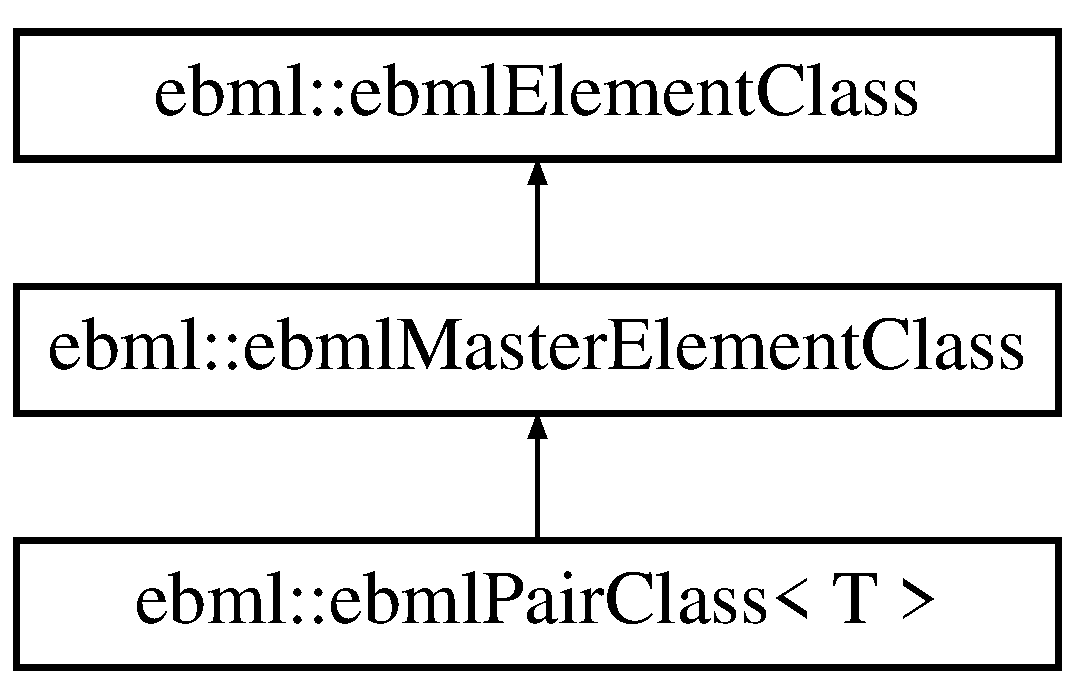
\includegraphics[height=3.000000cm]{classebml_1_1ebmlPairClass}
\end{center}
\end{figure}
\subsection*{Public Member Functions}
\begin{DoxyCompactItemize}
\item 
\mbox{\hyperlink{classebml_1_1ebmlPairClass_aeb7ee60aa846a317cecc39c5c79aeb2e}{ebml\+Pair\+Class}} (const char $\ast$, const std\+::wstring \&, const \mbox{\hyperlink{classebml_1_1ebmlElementClass}{ebml\+Element\+Class}} $\ast$\mbox{\hyperlink{classebml_1_1ebmlPairClass_a94538c4319b9d572bce2c05f6d999410}{keycls}}, const \mbox{\hyperlink{classebml_1_1ebmlElementClass}{ebml\+Element\+Class}} $\ast$\mbox{\hyperlink{classebml_1_1ebmlPairClass_ac4726d7f429838e8ec8e2d294b680a3d}{valcls}})
\item 
\mbox{\hyperlink{classebml_1_1ebmlPairClass_a2830fdd542ad3a6d25dba990956e0818}{ebml\+Pair\+Class}} (const char $\ast$, const std\+::wstring \&, const \mbox{\hyperlink{classebml_1_1ebmlDataElementClass}{ebml\+Data\+Element\+Class}}$<$ T $>$ $\ast$\mbox{\hyperlink{classebml_1_1ebmlPairClass_a94538c4319b9d572bce2c05f6d999410}{keycls}}, const \mbox{\hyperlink{classebml_1_1ebmlElementClass}{ebml\+Element\+Class}} $\ast$\mbox{\hyperlink{classebml_1_1ebmlPairClass_ac4726d7f429838e8ec8e2d294b680a3d}{valcls}})
\item 
\mbox{\hyperlink{classebml_1_1ebmlPairClass_ab1d08a05b102e555cb16e3416dda5fec}{ebml\+Pair\+Class}} (\mbox{\hyperlink{namespaceebml_a86c5f604ddf12a74aa9812e997a58691}{ebml\+I\+D\+\_\+t}}, const std\+::wstring \&, const \mbox{\hyperlink{classebml_1_1ebmlElementClass}{ebml\+Element\+Class}} $\ast$\mbox{\hyperlink{classebml_1_1ebmlPairClass_a94538c4319b9d572bce2c05f6d999410}{keycls}}, const \mbox{\hyperlink{classebml_1_1ebmlElementClass}{ebml\+Element\+Class}} $\ast$\mbox{\hyperlink{classebml_1_1ebmlPairClass_ac4726d7f429838e8ec8e2d294b680a3d}{valcls}})
\item 
\mbox{\hyperlink{classebml_1_1ebmlPairClass_a399efa1fe09fc7c381081a121cb039f7}{ebml\+Pair\+Class}} (\mbox{\hyperlink{namespaceebml_a86c5f604ddf12a74aa9812e997a58691}{ebml\+I\+D\+\_\+t}}, const std\+::wstring \&, const \mbox{\hyperlink{classebml_1_1ebmlDataElementClass}{ebml\+Data\+Element\+Class}}$<$ T $>$ $\ast$\mbox{\hyperlink{classebml_1_1ebmlPairClass_a94538c4319b9d572bce2c05f6d999410}{keycls}}, const \mbox{\hyperlink{classebml_1_1ebmlElementClass}{ebml\+Element\+Class}} $\ast$\mbox{\hyperlink{classebml_1_1ebmlPairClass_ac4726d7f429838e8ec8e2d294b680a3d}{valcls}})
\item 
\mbox{\hyperlink{namespaceebml_adad533b7705a16bb360fe56380c5e7be}{ebml\+Element\+\_\+sp}} \mbox{\hyperlink{classebml_1_1ebmlPairClass_a7f292456eaed4b0cebfbdd1c7f137444}{operator()}} (const \mbox{\hyperlink{namespaceebml_adad533b7705a16bb360fe56380c5e7be}{ebml\+Element\+\_\+sp}} \&, const \mbox{\hyperlink{namespaceebml_adad533b7705a16bb360fe56380c5e7be}{ebml\+Element\+\_\+sp}} \&) const
\item 
\mbox{\hyperlink{namespaceebml_adad533b7705a16bb360fe56380c5e7be}{ebml\+Element\+\_\+sp}} \mbox{\hyperlink{classebml_1_1ebmlPairClass_abe0424fbc5ad585ed11693f9d9f71f9e}{operator()}} (\mbox{\hyperlink{namespaceebml_adad533b7705a16bb360fe56380c5e7be}{ebml\+Element\+\_\+sp}} \&\&, \mbox{\hyperlink{namespaceebml_adad533b7705a16bb360fe56380c5e7be}{ebml\+Element\+\_\+sp}} \&\&) const
\item 
\mbox{\hyperlink{namespaceebml_adad533b7705a16bb360fe56380c5e7be}{ebml\+Element\+\_\+sp}} \mbox{\hyperlink{classebml_1_1ebmlPairClass_ab34a8f614bf92ab90fb37d178aaa0f0b}{operator()}} (const T \&, const \mbox{\hyperlink{namespaceebml_adad533b7705a16bb360fe56380c5e7be}{ebml\+Element\+\_\+sp}} \&) const
\item 
\mbox{\hyperlink{namespaceebml_adad533b7705a16bb360fe56380c5e7be}{ebml\+Element\+\_\+sp}} \mbox{\hyperlink{classebml_1_1ebmlPairClass_adf29892f267e47bd519b20811ed8e449}{operator()}} (const T \&, \mbox{\hyperlink{namespaceebml_adad533b7705a16bb360fe56380c5e7be}{ebml\+Element\+\_\+sp}} \&\&) const
\item 
\mbox{\hyperlink{namespaceebml_adad533b7705a16bb360fe56380c5e7be}{ebml\+Element\+\_\+sp}} \mbox{\hyperlink{classebml_1_1ebmlPairClass_abaeddeedcfdddb43a87175bf7f17dc31}{operator()}} (T \&\&, \mbox{\hyperlink{namespaceebml_adad533b7705a16bb360fe56380c5e7be}{ebml\+Element\+\_\+sp}} \&\&) const
\item 
const \mbox{\hyperlink{classebml_1_1ebmlDataElementClass}{ebml\+Data\+Element\+Class}}$<$ T $>$ $\ast$ \mbox{\hyperlink{classebml_1_1ebmlPairClass_a94538c4319b9d572bce2c05f6d999410}{keycls}} () const
\item 
const \mbox{\hyperlink{classebml_1_1ebmlElementClass}{ebml\+Element\+Class}} $\ast$ \mbox{\hyperlink{classebml_1_1ebmlPairClass_ac4726d7f429838e8ec8e2d294b680a3d}{valcls}} () const
\end{DoxyCompactItemize}
\subsection*{Protected Member Functions}
\begin{DoxyCompactItemize}
\item 
\mbox{\hyperlink{classebml_1_1ebmlElement}{ebml\+Element}} $\ast$ \mbox{\hyperlink{classebml_1_1ebmlPairClass_abb748027028719a4a1682c089ac21226}{\+\_\+new}} () const
\end{DoxyCompactItemize}
\subsection*{Protected Attributes}
\begin{DoxyCompactItemize}
\item 
\mbox{\hyperlink{classebml_1_1childClassSpec__t}{child\+Class\+Spec\+\_\+t}} \mbox{\hyperlink{classebml_1_1ebmlPairClass_ad560a3a9e6b47eb8e51e707de59df919}{\+\_\+value\+Spec}}
\end{DoxyCompactItemize}
\subsection*{Friends}
\begin{DoxyCompactItemize}
\item 
class \mbox{\hyperlink{classebml_1_1ebmlPairClass_ad1db4b5395f31070d1be2d251ee85e02}{ebml\+Pair$<$ T $>$}}
\end{DoxyCompactItemize}
\subsection*{Additional Inherited Members}


\subsection{Constructor \& Destructor Documentation}
\mbox{\Hypertarget{classebml_1_1ebmlPairClass_aeb7ee60aa846a317cecc39c5c79aeb2e}\label{classebml_1_1ebmlPairClass_aeb7ee60aa846a317cecc39c5c79aeb2e}} 
\index{ebml\+::ebml\+Pair\+Class@{ebml\+::ebml\+Pair\+Class}!ebml\+Pair\+Class@{ebml\+Pair\+Class}}
\index{ebml\+Pair\+Class@{ebml\+Pair\+Class}!ebml\+::ebml\+Pair\+Class@{ebml\+::ebml\+Pair\+Class}}
\subsubsection{\texorpdfstring{ebml\+Pair\+Class()}{ebmlPairClass()}\hspace{0.1cm}{\footnotesize\ttfamily [1/4]}}
{\footnotesize\ttfamily template$<$typename T$>$ \\
\mbox{\hyperlink{classebml_1_1ebmlPairClass}{ebml\+::ebml\+Pair\+Class}}$<$ T $>$\+::\mbox{\hyperlink{classebml_1_1ebmlPairClass}{ebml\+Pair\+Class}} (\begin{DoxyParamCaption}\item[{const char $\ast$}]{,  }\item[{const std\+::wstring \&}]{,  }\item[{const \mbox{\hyperlink{classebml_1_1ebmlElementClass}{ebml\+Element\+Class}} $\ast$}]{keycls,  }\item[{const \mbox{\hyperlink{classebml_1_1ebmlElementClass}{ebml\+Element\+Class}} $\ast$}]{valcls }\end{DoxyParamCaption})}

\mbox{\Hypertarget{classebml_1_1ebmlPairClass_a2830fdd542ad3a6d25dba990956e0818}\label{classebml_1_1ebmlPairClass_a2830fdd542ad3a6d25dba990956e0818}} 
\index{ebml\+::ebml\+Pair\+Class@{ebml\+::ebml\+Pair\+Class}!ebml\+Pair\+Class@{ebml\+Pair\+Class}}
\index{ebml\+Pair\+Class@{ebml\+Pair\+Class}!ebml\+::ebml\+Pair\+Class@{ebml\+::ebml\+Pair\+Class}}
\subsubsection{\texorpdfstring{ebml\+Pair\+Class()}{ebmlPairClass()}\hspace{0.1cm}{\footnotesize\ttfamily [2/4]}}
{\footnotesize\ttfamily template$<$typename T$>$ \\
\mbox{\hyperlink{classebml_1_1ebmlPairClass}{ebml\+::ebml\+Pair\+Class}}$<$ T $>$\+::\mbox{\hyperlink{classebml_1_1ebmlPairClass}{ebml\+Pair\+Class}} (\begin{DoxyParamCaption}\item[{const char $\ast$}]{,  }\item[{const std\+::wstring \&}]{,  }\item[{const \mbox{\hyperlink{classebml_1_1ebmlDataElementClass}{ebml\+Data\+Element\+Class}}$<$ T $>$ $\ast$}]{keycls,  }\item[{const \mbox{\hyperlink{classebml_1_1ebmlElementClass}{ebml\+Element\+Class}} $\ast$}]{valcls }\end{DoxyParamCaption})}

\mbox{\Hypertarget{classebml_1_1ebmlPairClass_ab1d08a05b102e555cb16e3416dda5fec}\label{classebml_1_1ebmlPairClass_ab1d08a05b102e555cb16e3416dda5fec}} 
\index{ebml\+::ebml\+Pair\+Class@{ebml\+::ebml\+Pair\+Class}!ebml\+Pair\+Class@{ebml\+Pair\+Class}}
\index{ebml\+Pair\+Class@{ebml\+Pair\+Class}!ebml\+::ebml\+Pair\+Class@{ebml\+::ebml\+Pair\+Class}}
\subsubsection{\texorpdfstring{ebml\+Pair\+Class()}{ebmlPairClass()}\hspace{0.1cm}{\footnotesize\ttfamily [3/4]}}
{\footnotesize\ttfamily template$<$typename T$>$ \\
\mbox{\hyperlink{classebml_1_1ebmlPairClass}{ebml\+::ebml\+Pair\+Class}}$<$ T $>$\+::\mbox{\hyperlink{classebml_1_1ebmlPairClass}{ebml\+Pair\+Class}} (\begin{DoxyParamCaption}\item[{\mbox{\hyperlink{namespaceebml_a86c5f604ddf12a74aa9812e997a58691}{ebml\+I\+D\+\_\+t}}}]{,  }\item[{const std\+::wstring \&}]{,  }\item[{const \mbox{\hyperlink{classebml_1_1ebmlElementClass}{ebml\+Element\+Class}} $\ast$}]{keycls,  }\item[{const \mbox{\hyperlink{classebml_1_1ebmlElementClass}{ebml\+Element\+Class}} $\ast$}]{valcls }\end{DoxyParamCaption})}

\mbox{\Hypertarget{classebml_1_1ebmlPairClass_a399efa1fe09fc7c381081a121cb039f7}\label{classebml_1_1ebmlPairClass_a399efa1fe09fc7c381081a121cb039f7}} 
\index{ebml\+::ebml\+Pair\+Class@{ebml\+::ebml\+Pair\+Class}!ebml\+Pair\+Class@{ebml\+Pair\+Class}}
\index{ebml\+Pair\+Class@{ebml\+Pair\+Class}!ebml\+::ebml\+Pair\+Class@{ebml\+::ebml\+Pair\+Class}}
\subsubsection{\texorpdfstring{ebml\+Pair\+Class()}{ebmlPairClass()}\hspace{0.1cm}{\footnotesize\ttfamily [4/4]}}
{\footnotesize\ttfamily template$<$typename T$>$ \\
\mbox{\hyperlink{classebml_1_1ebmlPairClass}{ebml\+::ebml\+Pair\+Class}}$<$ T $>$\+::\mbox{\hyperlink{classebml_1_1ebmlPairClass}{ebml\+Pair\+Class}} (\begin{DoxyParamCaption}\item[{\mbox{\hyperlink{namespaceebml_a86c5f604ddf12a74aa9812e997a58691}{ebml\+I\+D\+\_\+t}}}]{,  }\item[{const std\+::wstring \&}]{,  }\item[{const \mbox{\hyperlink{classebml_1_1ebmlDataElementClass}{ebml\+Data\+Element\+Class}}$<$ T $>$ $\ast$}]{keycls,  }\item[{const \mbox{\hyperlink{classebml_1_1ebmlElementClass}{ebml\+Element\+Class}} $\ast$}]{valcls }\end{DoxyParamCaption})}



\subsection{Member Function Documentation}
\mbox{\Hypertarget{classebml_1_1ebmlPairClass_abb748027028719a4a1682c089ac21226}\label{classebml_1_1ebmlPairClass_abb748027028719a4a1682c089ac21226}} 
\index{ebml\+::ebml\+Pair\+Class@{ebml\+::ebml\+Pair\+Class}!\+\_\+new@{\+\_\+new}}
\index{\+\_\+new@{\+\_\+new}!ebml\+::ebml\+Pair\+Class@{ebml\+::ebml\+Pair\+Class}}
\subsubsection{\texorpdfstring{\+\_\+new()}{\_new()}}
{\footnotesize\ttfamily template$<$typename T$>$ \\
\mbox{\hyperlink{classebml_1_1ebmlElement}{ebml\+Element}}$\ast$ \mbox{\hyperlink{classebml_1_1ebmlPairClass}{ebml\+::ebml\+Pair\+Class}}$<$ T $>$\+::\+\_\+new (\begin{DoxyParamCaption}{ }\end{DoxyParamCaption}) const\hspace{0.3cm}{\ttfamily [protected]}, {\ttfamily [virtual]}}



Implements \mbox{\hyperlink{classebml_1_1ebmlElementClass_a223ede6b8bc3c85251d2d73f0256fb45}{ebml\+::ebml\+Element\+Class}}.

\mbox{\Hypertarget{classebml_1_1ebmlPairClass_a94538c4319b9d572bce2c05f6d999410}\label{classebml_1_1ebmlPairClass_a94538c4319b9d572bce2c05f6d999410}} 
\index{ebml\+::ebml\+Pair\+Class@{ebml\+::ebml\+Pair\+Class}!keycls@{keycls}}
\index{keycls@{keycls}!ebml\+::ebml\+Pair\+Class@{ebml\+::ebml\+Pair\+Class}}
\subsubsection{\texorpdfstring{keycls()}{keycls()}}
{\footnotesize\ttfamily template$<$typename T$>$ \\
const \mbox{\hyperlink{classebml_1_1ebmlDataElementClass}{ebml\+Data\+Element\+Class}}$<$T$>$$\ast$ \mbox{\hyperlink{classebml_1_1ebmlPairClass}{ebml\+::ebml\+Pair\+Class}}$<$ T $>$\+::keycls (\begin{DoxyParamCaption}{ }\end{DoxyParamCaption}) const}

\mbox{\Hypertarget{classebml_1_1ebmlPairClass_a7f292456eaed4b0cebfbdd1c7f137444}\label{classebml_1_1ebmlPairClass_a7f292456eaed4b0cebfbdd1c7f137444}} 
\index{ebml\+::ebml\+Pair\+Class@{ebml\+::ebml\+Pair\+Class}!operator()@{operator()}}
\index{operator()@{operator()}!ebml\+::ebml\+Pair\+Class@{ebml\+::ebml\+Pair\+Class}}
\subsubsection{\texorpdfstring{operator()()}{operator()()}\hspace{0.1cm}{\footnotesize\ttfamily [1/5]}}
{\footnotesize\ttfamily template$<$typename T$>$ \\
\mbox{\hyperlink{namespaceebml_adad533b7705a16bb360fe56380c5e7be}{ebml\+Element\+\_\+sp}} \mbox{\hyperlink{classebml_1_1ebmlPairClass}{ebml\+::ebml\+Pair\+Class}}$<$ T $>$\+::operator() (\begin{DoxyParamCaption}\item[{const \mbox{\hyperlink{namespaceebml_adad533b7705a16bb360fe56380c5e7be}{ebml\+Element\+\_\+sp}} \&}]{,  }\item[{const \mbox{\hyperlink{namespaceebml_adad533b7705a16bb360fe56380c5e7be}{ebml\+Element\+\_\+sp}} \&}]{ }\end{DoxyParamCaption}) const}

\mbox{\Hypertarget{classebml_1_1ebmlPairClass_abe0424fbc5ad585ed11693f9d9f71f9e}\label{classebml_1_1ebmlPairClass_abe0424fbc5ad585ed11693f9d9f71f9e}} 
\index{ebml\+::ebml\+Pair\+Class@{ebml\+::ebml\+Pair\+Class}!operator()@{operator()}}
\index{operator()@{operator()}!ebml\+::ebml\+Pair\+Class@{ebml\+::ebml\+Pair\+Class}}
\subsubsection{\texorpdfstring{operator()()}{operator()()}\hspace{0.1cm}{\footnotesize\ttfamily [2/5]}}
{\footnotesize\ttfamily template$<$typename T$>$ \\
\mbox{\hyperlink{namespaceebml_adad533b7705a16bb360fe56380c5e7be}{ebml\+Element\+\_\+sp}} \mbox{\hyperlink{classebml_1_1ebmlPairClass}{ebml\+::ebml\+Pair\+Class}}$<$ T $>$\+::operator() (\begin{DoxyParamCaption}\item[{\mbox{\hyperlink{namespaceebml_adad533b7705a16bb360fe56380c5e7be}{ebml\+Element\+\_\+sp}} \&\&}]{,  }\item[{\mbox{\hyperlink{namespaceebml_adad533b7705a16bb360fe56380c5e7be}{ebml\+Element\+\_\+sp}} \&\&}]{ }\end{DoxyParamCaption}) const}

\mbox{\Hypertarget{classebml_1_1ebmlPairClass_ab34a8f614bf92ab90fb37d178aaa0f0b}\label{classebml_1_1ebmlPairClass_ab34a8f614bf92ab90fb37d178aaa0f0b}} 
\index{ebml\+::ebml\+Pair\+Class@{ebml\+::ebml\+Pair\+Class}!operator()@{operator()}}
\index{operator()@{operator()}!ebml\+::ebml\+Pair\+Class@{ebml\+::ebml\+Pair\+Class}}
\subsubsection{\texorpdfstring{operator()()}{operator()()}\hspace{0.1cm}{\footnotesize\ttfamily [3/5]}}
{\footnotesize\ttfamily template$<$typename T$>$ \\
\mbox{\hyperlink{namespaceebml_adad533b7705a16bb360fe56380c5e7be}{ebml\+Element\+\_\+sp}} \mbox{\hyperlink{classebml_1_1ebmlPairClass}{ebml\+::ebml\+Pair\+Class}}$<$ T $>$\+::operator() (\begin{DoxyParamCaption}\item[{const T \&}]{,  }\item[{const \mbox{\hyperlink{namespaceebml_adad533b7705a16bb360fe56380c5e7be}{ebml\+Element\+\_\+sp}} \&}]{ }\end{DoxyParamCaption}) const}

\mbox{\Hypertarget{classebml_1_1ebmlPairClass_adf29892f267e47bd519b20811ed8e449}\label{classebml_1_1ebmlPairClass_adf29892f267e47bd519b20811ed8e449}} 
\index{ebml\+::ebml\+Pair\+Class@{ebml\+::ebml\+Pair\+Class}!operator()@{operator()}}
\index{operator()@{operator()}!ebml\+::ebml\+Pair\+Class@{ebml\+::ebml\+Pair\+Class}}
\subsubsection{\texorpdfstring{operator()()}{operator()()}\hspace{0.1cm}{\footnotesize\ttfamily [4/5]}}
{\footnotesize\ttfamily template$<$typename T$>$ \\
\mbox{\hyperlink{namespaceebml_adad533b7705a16bb360fe56380c5e7be}{ebml\+Element\+\_\+sp}} \mbox{\hyperlink{classebml_1_1ebmlPairClass}{ebml\+::ebml\+Pair\+Class}}$<$ T $>$\+::operator() (\begin{DoxyParamCaption}\item[{const T \&}]{,  }\item[{\mbox{\hyperlink{namespaceebml_adad533b7705a16bb360fe56380c5e7be}{ebml\+Element\+\_\+sp}} \&\&}]{ }\end{DoxyParamCaption}) const}

\mbox{\Hypertarget{classebml_1_1ebmlPairClass_abaeddeedcfdddb43a87175bf7f17dc31}\label{classebml_1_1ebmlPairClass_abaeddeedcfdddb43a87175bf7f17dc31}} 
\index{ebml\+::ebml\+Pair\+Class@{ebml\+::ebml\+Pair\+Class}!operator()@{operator()}}
\index{operator()@{operator()}!ebml\+::ebml\+Pair\+Class@{ebml\+::ebml\+Pair\+Class}}
\subsubsection{\texorpdfstring{operator()()}{operator()()}\hspace{0.1cm}{\footnotesize\ttfamily [5/5]}}
{\footnotesize\ttfamily template$<$typename T$>$ \\
\mbox{\hyperlink{namespaceebml_adad533b7705a16bb360fe56380c5e7be}{ebml\+Element\+\_\+sp}} \mbox{\hyperlink{classebml_1_1ebmlPairClass}{ebml\+::ebml\+Pair\+Class}}$<$ T $>$\+::operator() (\begin{DoxyParamCaption}\item[{T \&\&}]{,  }\item[{\mbox{\hyperlink{namespaceebml_adad533b7705a16bb360fe56380c5e7be}{ebml\+Element\+\_\+sp}} \&\&}]{ }\end{DoxyParamCaption}) const}

\mbox{\Hypertarget{classebml_1_1ebmlPairClass_ac4726d7f429838e8ec8e2d294b680a3d}\label{classebml_1_1ebmlPairClass_ac4726d7f429838e8ec8e2d294b680a3d}} 
\index{ebml\+::ebml\+Pair\+Class@{ebml\+::ebml\+Pair\+Class}!valcls@{valcls}}
\index{valcls@{valcls}!ebml\+::ebml\+Pair\+Class@{ebml\+::ebml\+Pair\+Class}}
\subsubsection{\texorpdfstring{valcls()}{valcls()}}
{\footnotesize\ttfamily template$<$typename T$>$ \\
const \mbox{\hyperlink{classebml_1_1ebmlElementClass}{ebml\+Element\+Class}}$\ast$ \mbox{\hyperlink{classebml_1_1ebmlPairClass}{ebml\+::ebml\+Pair\+Class}}$<$ T $>$\+::valcls (\begin{DoxyParamCaption}{ }\end{DoxyParamCaption}) const}



\subsection{Friends And Related Function Documentation}
\mbox{\Hypertarget{classebml_1_1ebmlPairClass_ad1db4b5395f31070d1be2d251ee85e02}\label{classebml_1_1ebmlPairClass_ad1db4b5395f31070d1be2d251ee85e02}} 
\index{ebml\+::ebml\+Pair\+Class@{ebml\+::ebml\+Pair\+Class}!ebml\+Pair$<$ T $>$@{ebml\+Pair$<$ T $>$}}
\index{ebml\+Pair$<$ T $>$@{ebml\+Pair$<$ T $>$}!ebml\+::ebml\+Pair\+Class@{ebml\+::ebml\+Pair\+Class}}
\subsubsection{\texorpdfstring{ebml\+Pair$<$ T $>$}{ebmlPair< T >}}
{\footnotesize\ttfamily template$<$typename T$>$ \\
friend class \mbox{\hyperlink{classebml_1_1ebmlPair}{ebml\+Pair}}$<$ T $>$\hspace{0.3cm}{\ttfamily [friend]}}



\subsection{Member Data Documentation}
\mbox{\Hypertarget{classebml_1_1ebmlPairClass_ad560a3a9e6b47eb8e51e707de59df919}\label{classebml_1_1ebmlPairClass_ad560a3a9e6b47eb8e51e707de59df919}} 
\index{ebml\+::ebml\+Pair\+Class@{ebml\+::ebml\+Pair\+Class}!\+\_\+value\+Spec@{\+\_\+value\+Spec}}
\index{\+\_\+value\+Spec@{\+\_\+value\+Spec}!ebml\+::ebml\+Pair\+Class@{ebml\+::ebml\+Pair\+Class}}
\subsubsection{\texorpdfstring{\+\_\+value\+Spec}{\_valueSpec}}
{\footnotesize\ttfamily template$<$typename T$>$ \\
\mbox{\hyperlink{classebml_1_1childClassSpec__t}{child\+Class\+Spec\+\_\+t}} \mbox{\hyperlink{classebml_1_1ebmlPairClass}{ebml\+::ebml\+Pair\+Class}}$<$ T $>$\+::\+\_\+value\+Spec\hspace{0.3cm}{\ttfamily [protected]}}



The documentation for this class was generated from the following file\+:\begin{DoxyCompactItemize}
\item 
include/libebml\+\_\+ng/masterelement/\mbox{\hyperlink{map_8h}{map.\+h}}\end{DoxyCompactItemize}

\input{classebml_1_1ebmlSchema}
\hypertarget{classebml_1_1ebmlUnexpectedEndOfData}{}\section{ebml\+:\+:ebml\+Unexpected\+End\+Of\+Data Class Reference}
\label{classebml_1_1ebmlUnexpectedEndOfData}\index{ebml\+::ebml\+Unexpected\+End\+Of\+Data@{ebml\+::ebml\+Unexpected\+End\+Of\+Data}}


{\ttfamily \#include $<$exceptions.\+h$>$}

Inheritance diagram for ebml\+:\+:ebml\+Unexpected\+End\+Of\+Data\+:\begin{figure}[H]
\begin{center}
\leavevmode
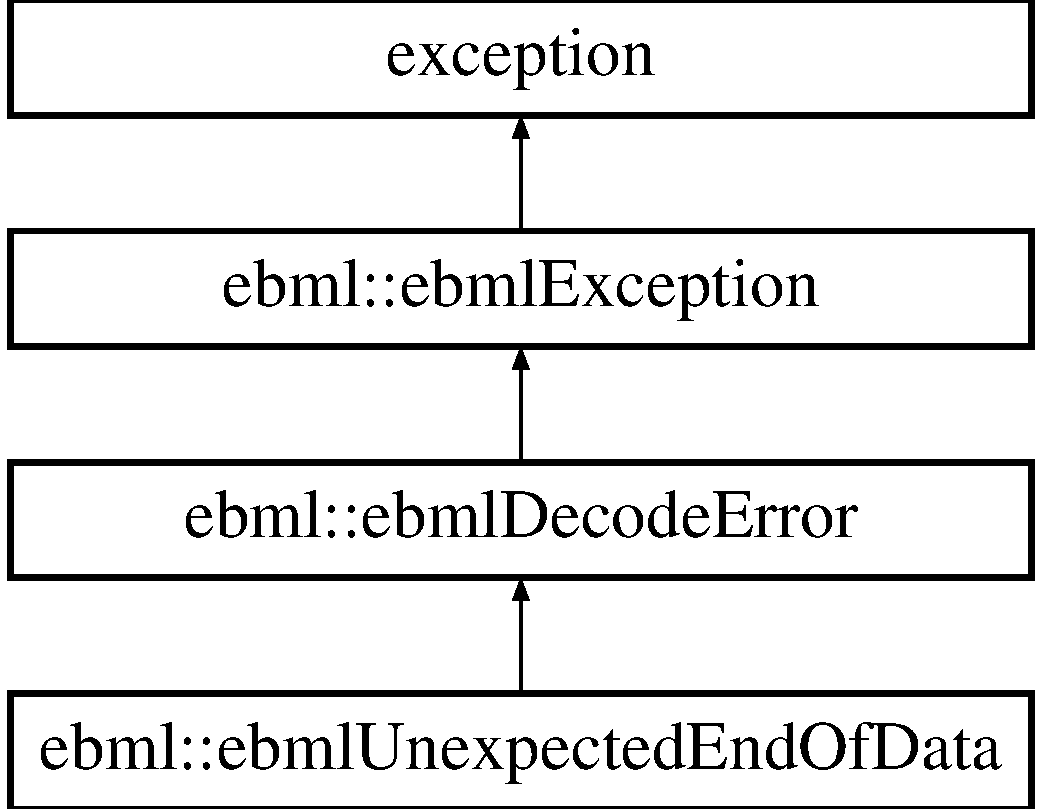
\includegraphics[height=4.000000cm]{classebml_1_1ebmlUnexpectedEndOfData}
\end{center}
\end{figure}
\subsection*{Public Member Functions}
\begin{DoxyCompactItemize}
\item 
\mbox{\hyperlink{classebml_1_1ebmlUnexpectedEndOfData_a4320d2a636ca459b356e15d496cca5ef}{ebml\+Unexpected\+End\+Of\+Data}} (const std\+::string \&message, const \mbox{\hyperlink{classebml_1_1ebmlElementClass}{ebml\+Element\+Class}} $\ast$\mbox{\hyperlink{classebml_1_1ebmlDecodeError_a3568b4ea3cd5bd16b9510abfe269920f}{cls}}=nullptr, off\+\_\+t \mbox{\hyperlink{classebml_1_1ebmlDecodeError_ad32ac9b3dd52f1c11479085d9c665e0f}{offset}}=-\/1, unsigned char \mbox{\hyperlink{classebml_1_1ebmlDecodeError_a61a4d4856f0c779a1c216e45dc5a7c1e}{head\+Size}}=0, off\+\_\+t \mbox{\hyperlink{classebml_1_1ebmlDecodeError_acb525117e0109d9640fb5e8c546e9a02}{erroroffset}}=-\/1)
\end{DoxyCompactItemize}
\subsection*{Additional Inherited Members}


\subsection{Constructor \& Destructor Documentation}
\mbox{\Hypertarget{classebml_1_1ebmlUnexpectedEndOfData_a4320d2a636ca459b356e15d496cca5ef}\label{classebml_1_1ebmlUnexpectedEndOfData_a4320d2a636ca459b356e15d496cca5ef}} 
\index{ebml\+::ebml\+Unexpected\+End\+Of\+Data@{ebml\+::ebml\+Unexpected\+End\+Of\+Data}!ebml\+Unexpected\+End\+Of\+Data@{ebml\+Unexpected\+End\+Of\+Data}}
\index{ebml\+Unexpected\+End\+Of\+Data@{ebml\+Unexpected\+End\+Of\+Data}!ebml\+::ebml\+Unexpected\+End\+Of\+Data@{ebml\+::ebml\+Unexpected\+End\+Of\+Data}}
\subsubsection{\texorpdfstring{ebml\+Unexpected\+End\+Of\+Data()}{ebmlUnexpectedEndOfData()}}
{\footnotesize\ttfamily ebml\+::ebml\+Unexpected\+End\+Of\+Data\+::ebml\+Unexpected\+End\+Of\+Data (\begin{DoxyParamCaption}\item[{const std\+::string \&}]{message,  }\item[{const \mbox{\hyperlink{classebml_1_1ebmlElementClass}{ebml\+Element\+Class}} $\ast$}]{cls = {\ttfamily nullptr},  }\item[{off\+\_\+t}]{offset = {\ttfamily -\/1},  }\item[{unsigned char}]{head\+Size = {\ttfamily 0},  }\item[{off\+\_\+t}]{erroroffset = {\ttfamily -\/1} }\end{DoxyParamCaption})}



The documentation for this class was generated from the following file\+:\begin{DoxyCompactItemize}
\item 
include/libebml\+\_\+ng/\mbox{\hyperlink{exceptions_8h}{exceptions.\+h}}\end{DoxyCompactItemize}

\hypertarget{classebml_1_1ebmlVoid}{}\section{ebml\+:\+:ebml\+Void Class Reference}
\label{classebml_1_1ebmlVoid}\index{ebml\+::ebml\+Void@{ebml\+::ebml\+Void}}


{\ttfamily \#include $<$void.\+h$>$}

Inheritance diagram for ebml\+:\+:ebml\+Void\+:\begin{figure}[H]
\begin{center}
\leavevmode
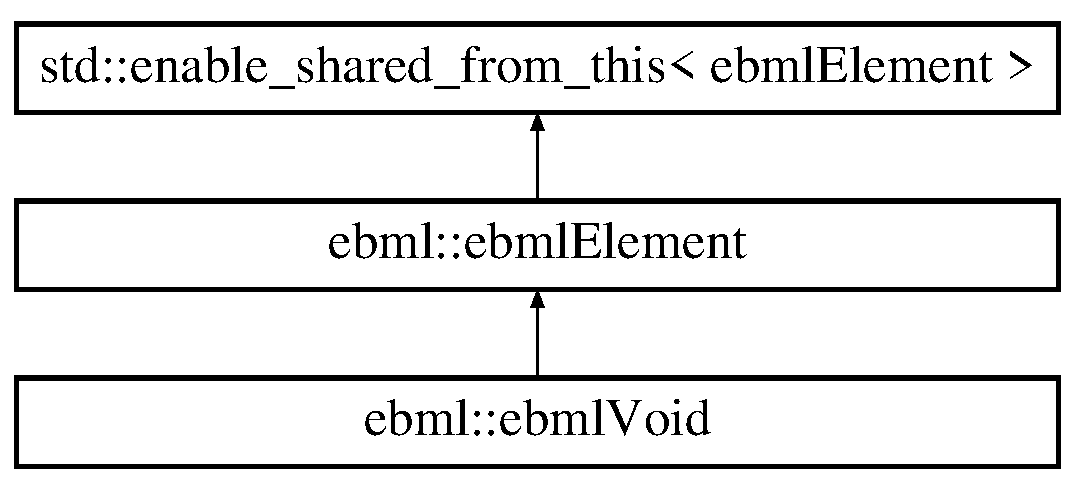
\includegraphics[height=3.000000cm]{classebml_1_1ebmlVoid}
\end{center}
\end{figure}
\subsection*{Public Member Functions}
\begin{DoxyCompactItemize}
\item 
size\+\_\+t \mbox{\hyperlink{classebml_1_1ebmlVoid_a9801f10eb9f0a5449fa39d8a31dbf315}{data\+Size}} () const
\item 
size\+\_\+t \mbox{\hyperlink{classebml_1_1ebmlVoid_ac822d7bf461ef44812596a34cccb134a}{encode}} (\mbox{\hyperlink{classebml_1_1ioBase}{io\+Base}} $\ast$) const
\item 
std\+::wstring \mbox{\hyperlink{classebml_1_1ebmlVoid_ad9baeb00b771d3ae4cdebb2078f863ad}{minirepr}} () const
\item 
std\+::wstring \mbox{\hyperlink{classebml_1_1ebmlVoid_a54f5a77bc4029d77d0a456fa8dcb53ef}{repr}} () const
\end{DoxyCompactItemize}
\subsection*{Public Attributes}
\begin{DoxyCompactItemize}
\item 
size\+\_\+t \mbox{\hyperlink{classebml_1_1ebmlVoid_a62a54e4b5ef5acf454f0240db8ee6c90}{voidsize}}
\end{DoxyCompactItemize}
\subsection*{Protected Member Functions}
\begin{DoxyCompactItemize}
\item 
\mbox{\hyperlink{classebml_1_1ebmlVoid_a3d6c579df46368e2b7bc78baab53c437}{ebml\+Void}} (const \mbox{\hyperlink{classebml_1_1ebmlVoidClass}{ebml\+Void\+Class}} $\ast$)
\item 
\mbox{\hyperlink{classebml_1_1ebmlVoid_a8f029c869cc3f14d1eea3c358e56bf1a}{ebml\+Void}} (const \mbox{\hyperlink{classebml_1_1ebmlVoidClass}{ebml\+Void\+Class}} $\ast$, size\+\_\+t)
\item 
size\+\_\+t \mbox{\hyperlink{classebml_1_1ebmlVoid_a58183338cb3b41b188cddfbb09a281d5}{\+\_\+encode}} (char $\ast$) const
\item 
void \mbox{\hyperlink{classebml_1_1ebmlVoid_a4d5d56b3b45c18c5732a4e0d68762f87}{\+\_\+decode}} (const \mbox{\hyperlink{classebml_1_1parseString}{parse\+String}} \&)
\item 
void \mbox{\hyperlink{classebml_1_1ebmlVoid_a3bf4c4cb979b33f513fd224329aee162}{\+\_\+decode}} (const \mbox{\hyperlink{classebml_1_1parseFile}{parse\+File}} \&)
\item 
void \mbox{\hyperlink{classebml_1_1ebmlVoid_a1319a15cbec91a7f52763c30d7fa3a18}{\+\_\+clonedata}} (const \mbox{\hyperlink{classebml_1_1ebmlElement}{ebml\+Element}} $\ast$)
\end{DoxyCompactItemize}
\subsection*{Friends}
\begin{DoxyCompactItemize}
\item 
class \mbox{\hyperlink{classebml_1_1ebmlVoid_ac7fd92f117d3b9c559a6d1725f579f9b}{ebml\+Void\+Class}}
\end{DoxyCompactItemize}
\subsection*{Additional Inherited Members}


\subsection{Constructor \& Destructor Documentation}
\mbox{\Hypertarget{classebml_1_1ebmlVoid_a3d6c579df46368e2b7bc78baab53c437}\label{classebml_1_1ebmlVoid_a3d6c579df46368e2b7bc78baab53c437}} 
\index{ebml\+::ebml\+Void@{ebml\+::ebml\+Void}!ebml\+Void@{ebml\+Void}}
\index{ebml\+Void@{ebml\+Void}!ebml\+::ebml\+Void@{ebml\+::ebml\+Void}}
\subsubsection{\texorpdfstring{ebml\+Void()}{ebmlVoid()}\hspace{0.1cm}{\footnotesize\ttfamily [1/2]}}
{\footnotesize\ttfamily ebml\+::ebml\+Void\+::ebml\+Void (\begin{DoxyParamCaption}\item[{const \mbox{\hyperlink{classebml_1_1ebmlVoidClass}{ebml\+Void\+Class}} $\ast$}]{ }\end{DoxyParamCaption})\hspace{0.3cm}{\ttfamily [protected]}}

\mbox{\Hypertarget{classebml_1_1ebmlVoid_a8f029c869cc3f14d1eea3c358e56bf1a}\label{classebml_1_1ebmlVoid_a8f029c869cc3f14d1eea3c358e56bf1a}} 
\index{ebml\+::ebml\+Void@{ebml\+::ebml\+Void}!ebml\+Void@{ebml\+Void}}
\index{ebml\+Void@{ebml\+Void}!ebml\+::ebml\+Void@{ebml\+::ebml\+Void}}
\subsubsection{\texorpdfstring{ebml\+Void()}{ebmlVoid()}\hspace{0.1cm}{\footnotesize\ttfamily [2/2]}}
{\footnotesize\ttfamily ebml\+::ebml\+Void\+::ebml\+Void (\begin{DoxyParamCaption}\item[{const \mbox{\hyperlink{classebml_1_1ebmlVoidClass}{ebml\+Void\+Class}} $\ast$}]{,  }\item[{size\+\_\+t}]{ }\end{DoxyParamCaption})\hspace{0.3cm}{\ttfamily [protected]}}



\subsection{Member Function Documentation}
\mbox{\Hypertarget{classebml_1_1ebmlVoid_a1319a15cbec91a7f52763c30d7fa3a18}\label{classebml_1_1ebmlVoid_a1319a15cbec91a7f52763c30d7fa3a18}} 
\index{ebml\+::ebml\+Void@{ebml\+::ebml\+Void}!\+\_\+clonedata@{\+\_\+clonedata}}
\index{\+\_\+clonedata@{\+\_\+clonedata}!ebml\+::ebml\+Void@{ebml\+::ebml\+Void}}
\subsubsection{\texorpdfstring{\+\_\+clonedata()}{\_clonedata()}}
{\footnotesize\ttfamily void ebml\+::ebml\+Void\+::\+\_\+clonedata (\begin{DoxyParamCaption}\item[{const \mbox{\hyperlink{classebml_1_1ebmlElement}{ebml\+Element}} $\ast$}]{ }\end{DoxyParamCaption})\hspace{0.3cm}{\ttfamily [protected]}, {\ttfamily [virtual]}}



Implements \mbox{\hyperlink{classebml_1_1ebmlElement_a3ebe3aa75b62971f385c01f27c807a02}{ebml\+::ebml\+Element}}.

\mbox{\Hypertarget{classebml_1_1ebmlVoid_a4d5d56b3b45c18c5732a4e0d68762f87}\label{classebml_1_1ebmlVoid_a4d5d56b3b45c18c5732a4e0d68762f87}} 
\index{ebml\+::ebml\+Void@{ebml\+::ebml\+Void}!\+\_\+decode@{\+\_\+decode}}
\index{\+\_\+decode@{\+\_\+decode}!ebml\+::ebml\+Void@{ebml\+::ebml\+Void}}
\subsubsection{\texorpdfstring{\+\_\+decode()}{\_decode()}\hspace{0.1cm}{\footnotesize\ttfamily [1/2]}}
{\footnotesize\ttfamily void ebml\+::ebml\+Void\+::\+\_\+decode (\begin{DoxyParamCaption}\item[{const \mbox{\hyperlink{classebml_1_1parseString}{parse\+String}} \&}]{ }\end{DoxyParamCaption})\hspace{0.3cm}{\ttfamily [protected]}}

\mbox{\Hypertarget{classebml_1_1ebmlVoid_a3bf4c4cb979b33f513fd224329aee162}\label{classebml_1_1ebmlVoid_a3bf4c4cb979b33f513fd224329aee162}} 
\index{ebml\+::ebml\+Void@{ebml\+::ebml\+Void}!\+\_\+decode@{\+\_\+decode}}
\index{\+\_\+decode@{\+\_\+decode}!ebml\+::ebml\+Void@{ebml\+::ebml\+Void}}
\subsubsection{\texorpdfstring{\+\_\+decode()}{\_decode()}\hspace{0.1cm}{\footnotesize\ttfamily [2/2]}}
{\footnotesize\ttfamily void ebml\+::ebml\+Void\+::\+\_\+decode (\begin{DoxyParamCaption}\item[{const \mbox{\hyperlink{classebml_1_1parseFile}{parse\+File}} \&}]{ }\end{DoxyParamCaption})\hspace{0.3cm}{\ttfamily [protected]}}

\mbox{\Hypertarget{classebml_1_1ebmlVoid_a58183338cb3b41b188cddfbb09a281d5}\label{classebml_1_1ebmlVoid_a58183338cb3b41b188cddfbb09a281d5}} 
\index{ebml\+::ebml\+Void@{ebml\+::ebml\+Void}!\+\_\+encode@{\+\_\+encode}}
\index{\+\_\+encode@{\+\_\+encode}!ebml\+::ebml\+Void@{ebml\+::ebml\+Void}}
\subsubsection{\texorpdfstring{\+\_\+encode()}{\_encode()}}
{\footnotesize\ttfamily size\+\_\+t ebml\+::ebml\+Void\+::\+\_\+encode (\begin{DoxyParamCaption}\item[{char $\ast$}]{ }\end{DoxyParamCaption}) const\hspace{0.3cm}{\ttfamily [protected]}, {\ttfamily [virtual]}}



Implements \mbox{\hyperlink{classebml_1_1ebmlElement_a27bd9de14e1706840235b68331917776}{ebml\+::ebml\+Element}}.

\mbox{\Hypertarget{classebml_1_1ebmlVoid_a9801f10eb9f0a5449fa39d8a31dbf315}\label{classebml_1_1ebmlVoid_a9801f10eb9f0a5449fa39d8a31dbf315}} 
\index{ebml\+::ebml\+Void@{ebml\+::ebml\+Void}!data\+Size@{data\+Size}}
\index{data\+Size@{data\+Size}!ebml\+::ebml\+Void@{ebml\+::ebml\+Void}}
\subsubsection{\texorpdfstring{data\+Size()}{dataSize()}}
{\footnotesize\ttfamily size\+\_\+t ebml\+::ebml\+Void\+::data\+Size (\begin{DoxyParamCaption}{ }\end{DoxyParamCaption}) const\hspace{0.3cm}{\ttfamily [virtual]}}



Implements \mbox{\hyperlink{classebml_1_1ebmlElement_a47ed4167d9c69104e02b6dbad0cd1fef}{ebml\+::ebml\+Element}}.

\mbox{\Hypertarget{classebml_1_1ebmlVoid_ac822d7bf461ef44812596a34cccb134a}\label{classebml_1_1ebmlVoid_ac822d7bf461ef44812596a34cccb134a}} 
\index{ebml\+::ebml\+Void@{ebml\+::ebml\+Void}!encode@{encode}}
\index{encode@{encode}!ebml\+::ebml\+Void@{ebml\+::ebml\+Void}}
\subsubsection{\texorpdfstring{encode()}{encode()}}
{\footnotesize\ttfamily size\+\_\+t ebml\+::ebml\+Void\+::encode (\begin{DoxyParamCaption}\item[{\mbox{\hyperlink{classebml_1_1ioBase}{io\+Base}} $\ast$}]{ }\end{DoxyParamCaption}) const\hspace{0.3cm}{\ttfamily [virtual]}}



Reimplemented from \mbox{\hyperlink{classebml_1_1ebmlElement_ad493e4103807b8d4434c0667c148dcea}{ebml\+::ebml\+Element}}.

\mbox{\Hypertarget{classebml_1_1ebmlVoid_ad9baeb00b771d3ae4cdebb2078f863ad}\label{classebml_1_1ebmlVoid_ad9baeb00b771d3ae4cdebb2078f863ad}} 
\index{ebml\+::ebml\+Void@{ebml\+::ebml\+Void}!minirepr@{minirepr}}
\index{minirepr@{minirepr}!ebml\+::ebml\+Void@{ebml\+::ebml\+Void}}
\subsubsection{\texorpdfstring{minirepr()}{minirepr()}}
{\footnotesize\ttfamily std\+::wstring ebml\+::ebml\+Void\+::minirepr (\begin{DoxyParamCaption}{ }\end{DoxyParamCaption}) const\hspace{0.3cm}{\ttfamily [virtual]}}



Implements \mbox{\hyperlink{classebml_1_1ebmlElement_a7852173aeef78bd843939ae5a82f1d1c}{ebml\+::ebml\+Element}}.

\mbox{\Hypertarget{classebml_1_1ebmlVoid_a54f5a77bc4029d77d0a456fa8dcb53ef}\label{classebml_1_1ebmlVoid_a54f5a77bc4029d77d0a456fa8dcb53ef}} 
\index{ebml\+::ebml\+Void@{ebml\+::ebml\+Void}!repr@{repr}}
\index{repr@{repr}!ebml\+::ebml\+Void@{ebml\+::ebml\+Void}}
\subsubsection{\texorpdfstring{repr()}{repr()}}
{\footnotesize\ttfamily std\+::wstring ebml\+::ebml\+Void\+::repr (\begin{DoxyParamCaption}{ }\end{DoxyParamCaption}) const\hspace{0.3cm}{\ttfamily [virtual]}}



Reimplemented from \mbox{\hyperlink{classebml_1_1ebmlElement_a77865a71f4bab782817ec82e88fb5198}{ebml\+::ebml\+Element}}.



\subsection{Friends And Related Function Documentation}
\mbox{\Hypertarget{classebml_1_1ebmlVoid_ac7fd92f117d3b9c559a6d1725f579f9b}\label{classebml_1_1ebmlVoid_ac7fd92f117d3b9c559a6d1725f579f9b}} 
\index{ebml\+::ebml\+Void@{ebml\+::ebml\+Void}!ebml\+Void\+Class@{ebml\+Void\+Class}}
\index{ebml\+Void\+Class@{ebml\+Void\+Class}!ebml\+::ebml\+Void@{ebml\+::ebml\+Void}}
\subsubsection{\texorpdfstring{ebml\+Void\+Class}{ebmlVoidClass}}
{\footnotesize\ttfamily friend class \mbox{\hyperlink{classebml_1_1ebmlVoidClass}{ebml\+Void\+Class}}\hspace{0.3cm}{\ttfamily [friend]}}



\subsection{Member Data Documentation}
\mbox{\Hypertarget{classebml_1_1ebmlVoid_a62a54e4b5ef5acf454f0240db8ee6c90}\label{classebml_1_1ebmlVoid_a62a54e4b5ef5acf454f0240db8ee6c90}} 
\index{ebml\+::ebml\+Void@{ebml\+::ebml\+Void}!voidsize@{voidsize}}
\index{voidsize@{voidsize}!ebml\+::ebml\+Void@{ebml\+::ebml\+Void}}
\subsubsection{\texorpdfstring{voidsize}{voidsize}}
{\footnotesize\ttfamily size\+\_\+t ebml\+::ebml\+Void\+::voidsize}



The documentation for this class was generated from the following file\+:\begin{DoxyCompactItemize}
\item 
include/libebml\+\_\+ng/\mbox{\hyperlink{void_8h}{void.\+h}}\end{DoxyCompactItemize}

\hypertarget{classebml_1_1ebmlVoidClass}{}\section{ebml\+:\+:ebml\+Void\+Class Class Reference}
\label{classebml_1_1ebmlVoidClass}\index{ebml\+::ebml\+Void\+Class@{ebml\+::ebml\+Void\+Class}}


{\ttfamily \#include $<$base.\+h$>$}

Inheritance diagram for ebml\+:\+:ebml\+Void\+Class\+:\begin{figure}[H]
\begin{center}
\leavevmode
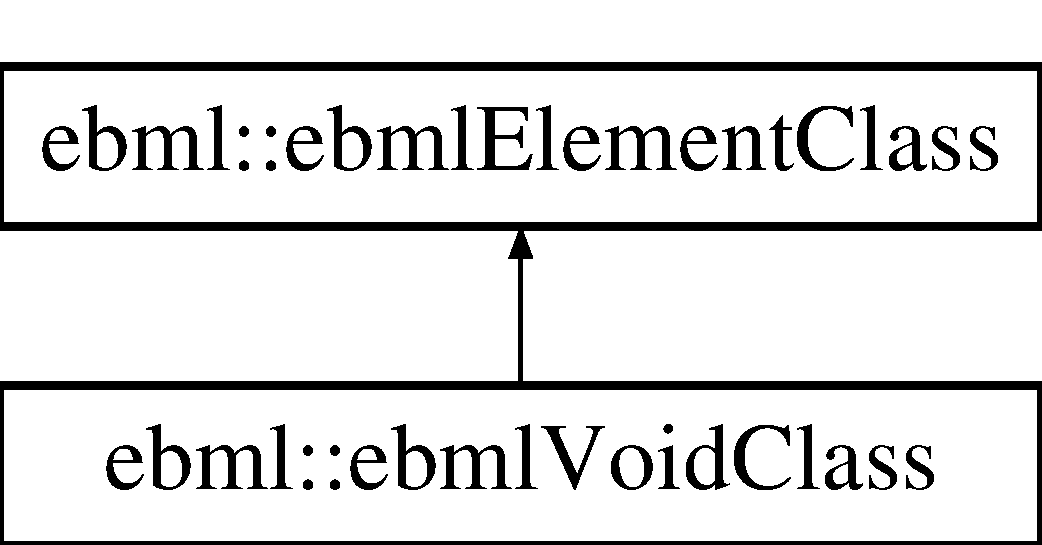
\includegraphics[height=2.000000cm]{classebml_1_1ebmlVoidClass}
\end{center}
\end{figure}
\subsection*{Public Member Functions}
\begin{DoxyCompactItemize}
\item 
\mbox{\hyperlink{classebml_1_1ebmlVoidClass_afc8666d6bbcd41bad76bfc5a2b5b4c9a}{ebml\+Void\+Class}} ()
\item 
\mbox{\hyperlink{namespaceebml_adad533b7705a16bb360fe56380c5e7be}{ebml\+Element\+\_\+sp}} \mbox{\hyperlink{classebml_1_1ebmlVoidClass_ad570c8614bf8fc88edecbbe0d3a335e6}{operator()}} (size\+\_\+t) const
\end{DoxyCompactItemize}
\subsection*{Protected Member Functions}
\begin{DoxyCompactItemize}
\item 
\mbox{\hyperlink{classebml_1_1ebmlElement}{ebml\+Element}} $\ast$ \mbox{\hyperlink{classebml_1_1ebmlVoidClass_a8852efa478e785ae70b4fce60f67e6f7}{\+\_\+new}} () const
\end{DoxyCompactItemize}
\subsection*{Friends}
\begin{DoxyCompactItemize}
\item 
class \mbox{\hyperlink{classebml_1_1ebmlVoidClass_af2d556fe3de73937062cdd59bad2a1c0}{ebml\+Void}}
\end{DoxyCompactItemize}
\subsection*{Additional Inherited Members}


\subsection{Constructor \& Destructor Documentation}
\mbox{\Hypertarget{classebml_1_1ebmlVoidClass_afc8666d6bbcd41bad76bfc5a2b5b4c9a}\label{classebml_1_1ebmlVoidClass_afc8666d6bbcd41bad76bfc5a2b5b4c9a}} 
\index{ebml\+::ebml\+Void\+Class@{ebml\+::ebml\+Void\+Class}!ebml\+Void\+Class@{ebml\+Void\+Class}}
\index{ebml\+Void\+Class@{ebml\+Void\+Class}!ebml\+::ebml\+Void\+Class@{ebml\+::ebml\+Void\+Class}}
\subsubsection{\texorpdfstring{ebml\+Void\+Class()}{ebmlVoidClass()}}
{\footnotesize\ttfamily ebml\+::ebml\+Void\+Class\+::ebml\+Void\+Class (\begin{DoxyParamCaption}{ }\end{DoxyParamCaption})}



\subsection{Member Function Documentation}
\mbox{\Hypertarget{classebml_1_1ebmlVoidClass_a8852efa478e785ae70b4fce60f67e6f7}\label{classebml_1_1ebmlVoidClass_a8852efa478e785ae70b4fce60f67e6f7}} 
\index{ebml\+::ebml\+Void\+Class@{ebml\+::ebml\+Void\+Class}!\+\_\+new@{\+\_\+new}}
\index{\+\_\+new@{\+\_\+new}!ebml\+::ebml\+Void\+Class@{ebml\+::ebml\+Void\+Class}}
\subsubsection{\texorpdfstring{\+\_\+new()}{\_new()}}
{\footnotesize\ttfamily \mbox{\hyperlink{classebml_1_1ebmlElement}{ebml\+Element}}$\ast$ ebml\+::ebml\+Void\+Class\+::\+\_\+new (\begin{DoxyParamCaption}{ }\end{DoxyParamCaption}) const\hspace{0.3cm}{\ttfamily [protected]}, {\ttfamily [virtual]}}



Implements \mbox{\hyperlink{classebml_1_1ebmlElementClass_a223ede6b8bc3c85251d2d73f0256fb45}{ebml\+::ebml\+Element\+Class}}.

\mbox{\Hypertarget{classebml_1_1ebmlVoidClass_ad570c8614bf8fc88edecbbe0d3a335e6}\label{classebml_1_1ebmlVoidClass_ad570c8614bf8fc88edecbbe0d3a335e6}} 
\index{ebml\+::ebml\+Void\+Class@{ebml\+::ebml\+Void\+Class}!operator()@{operator()}}
\index{operator()@{operator()}!ebml\+::ebml\+Void\+Class@{ebml\+::ebml\+Void\+Class}}
\subsubsection{\texorpdfstring{operator()()}{operator()()}}
{\footnotesize\ttfamily \mbox{\hyperlink{namespaceebml_adad533b7705a16bb360fe56380c5e7be}{ebml\+Element\+\_\+sp}} ebml\+::ebml\+Void\+Class\+::operator() (\begin{DoxyParamCaption}\item[{size\+\_\+t}]{ }\end{DoxyParamCaption}) const}



\subsection{Friends And Related Function Documentation}
\mbox{\Hypertarget{classebml_1_1ebmlVoidClass_af2d556fe3de73937062cdd59bad2a1c0}\label{classebml_1_1ebmlVoidClass_af2d556fe3de73937062cdd59bad2a1c0}} 
\index{ebml\+::ebml\+Void\+Class@{ebml\+::ebml\+Void\+Class}!ebml\+Void@{ebml\+Void}}
\index{ebml\+Void@{ebml\+Void}!ebml\+::ebml\+Void\+Class@{ebml\+::ebml\+Void\+Class}}
\subsubsection{\texorpdfstring{ebml\+Void}{ebmlVoid}}
{\footnotesize\ttfamily friend class \mbox{\hyperlink{classebml_1_1ebmlVoid}{ebml\+Void}}\hspace{0.3cm}{\ttfamily [friend]}}



The documentation for this class was generated from the following file\+:\begin{DoxyCompactItemize}
\item 
include/libebml\+\_\+ng/\mbox{\hyperlink{base_8h}{base.\+h}}\end{DoxyCompactItemize}

\hypertarget{classebml_1_1io}{}\section{ebml\+:\+:io$<$ T $>$ Class Template Reference}
\label{classebml_1_1io}\index{ebml\+::io$<$ T $>$@{ebml\+::io$<$ T $>$}}


{\ttfamily \#include $<$io.\+h$>$}

Inheritance diagram for ebml\+:\+:io$<$ T $>$\+:\begin{figure}[H]
\begin{center}
\leavevmode
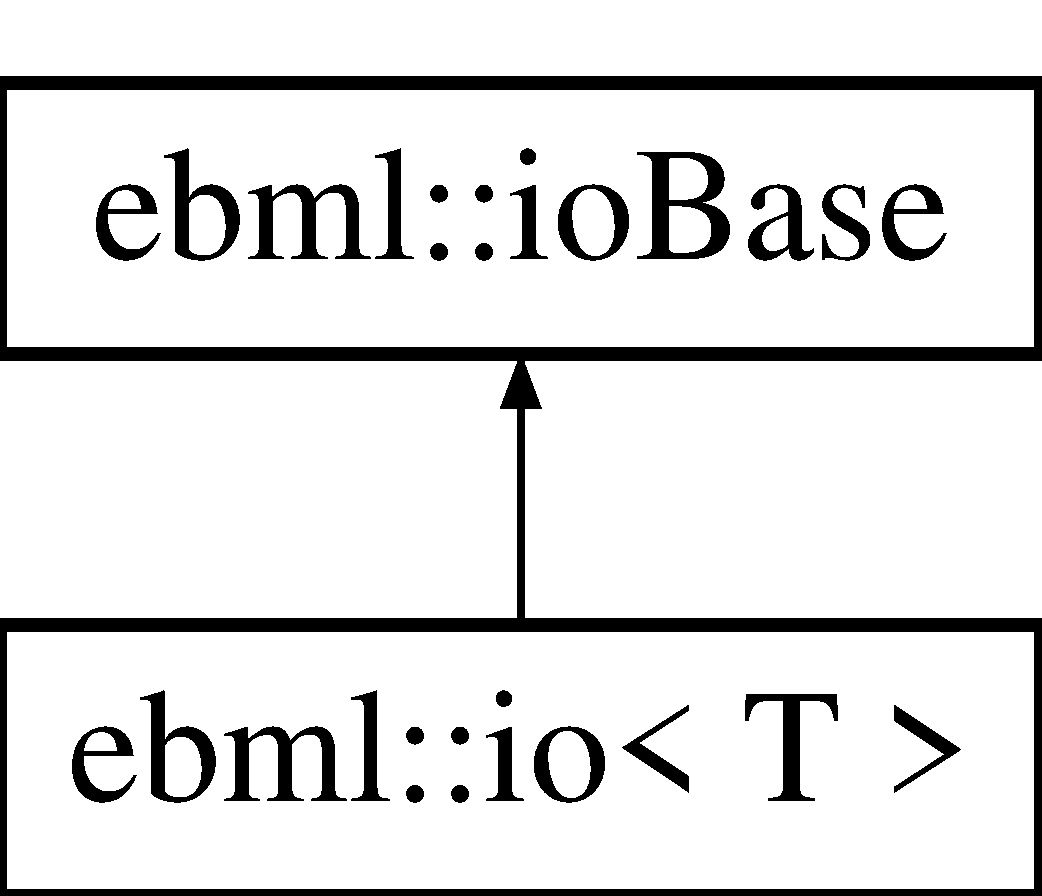
\includegraphics[height=2.000000cm]{classebml_1_1io}
\end{center}
\end{figure}
\subsection*{Public Member Functions}
\begin{DoxyCompactItemize}
\item 
\mbox{\hyperlink{classebml_1_1io_acf15f9f08eb2e65c72363320aa8bc112}{io}} (T)
\item 
std\+::ios\+\_\+base\+::openmode \mbox{\hyperlink{classebml_1_1io_ab1143b5c835958387d95695151744d33}{mode}} () const
\item 
bool \mbox{\hyperlink{classebml_1_1io_ab019a4128b3339941124a12632c919fd}{seekable}} ()
\item 
size\+\_\+t \mbox{\hyperlink{classebml_1_1io_ad745dc2c29544750dcd38a21cba0a16c}{read}} (char $\ast$, off\+\_\+t, size\+\_\+t)
\item 
size\+\_\+t \mbox{\hyperlink{classebml_1_1io_a5c3f2df6edfbd090b4d0fbc8a6dacccb}{write}} (const char $\ast$, off\+\_\+t, size\+\_\+t)
\item 
void \mbox{\hyperlink{classebml_1_1io_a6a5c0f2182844094c6b4432a15adccc8}{truncate}} ()
\item 
void \mbox{\hyperlink{classebml_1_1io_a9a50a99136e7e9a4a404dc3087024a7f}{truncate}} (off\+\_\+t)
\item 
void \mbox{\hyperlink{classebml_1_1io_a929714d05587d37d46bf8813b35c788d}{close}} ()
\item 
{\footnotesize template$<$$>$ }\\bool \mbox{\hyperlink{classebml_1_1io_a6e97c1e6868bf65286328b9447eaa419}{seekable}} ()
\item 
{\footnotesize template$<$$>$ }\\size\+\_\+t \mbox{\hyperlink{classebml_1_1io_a3b291aa8fb7bbeeb3f9d2ef152c37115}{read}} (char $\ast$, off\+\_\+t, size\+\_\+t)
\item 
{\footnotesize template$<$$>$ }\\size\+\_\+t \mbox{\hyperlink{classebml_1_1io_aedbdf5a69ee0ae64f909a59645cd0db7}{write}} (const char $\ast$, off\+\_\+t, size\+\_\+t)
\item 
{\footnotesize template$<$$>$ }\\bool \mbox{\hyperlink{classebml_1_1io_a4ea6caf18c5646646b3a15bc3c59a5ab}{seekable}} ()
\end{DoxyCompactItemize}
\subsection*{Static Public Member Functions}
\begin{DoxyCompactItemize}
\item 
static \mbox{\hyperlink{namespaceebml_a7bb59128ac6af27e47367938a846b569}{io\+Base\+\_\+sp}} \mbox{\hyperlink{classebml_1_1io_a722fbb02777e4af8e42779750c588f63}{wrap}} (T)
\item 
static \mbox{\hyperlink{namespaceebml_a7bb59128ac6af27e47367938a846b569}{io\+Base\+\_\+sp}} \mbox{\hyperlink{classebml_1_1io_a98871b6a6ceafc80df00f95867b7cbe4}{open}} (const std\+::string \&, const std\+::ios\+\_\+base\+::openmode \&)
\end{DoxyCompactItemize}
\subsection*{Additional Inherited Members}


\subsection{Constructor \& Destructor Documentation}
\mbox{\Hypertarget{classebml_1_1io_acf15f9f08eb2e65c72363320aa8bc112}\label{classebml_1_1io_acf15f9f08eb2e65c72363320aa8bc112}} 
\index{ebml\+::io@{ebml\+::io}!io@{io}}
\index{io@{io}!ebml\+::io@{ebml\+::io}}
\subsubsection{\texorpdfstring{io()}{io()}}
{\footnotesize\ttfamily template$<$typename T $>$ \\
\mbox{\hyperlink{classebml_1_1io}{ebml\+::io}}$<$ T $>$\+::\mbox{\hyperlink{classebml_1_1io}{io}} (\begin{DoxyParamCaption}\item[{T}]{ }\end{DoxyParamCaption})}



\subsection{Member Function Documentation}
\mbox{\Hypertarget{classebml_1_1io_a929714d05587d37d46bf8813b35c788d}\label{classebml_1_1io_a929714d05587d37d46bf8813b35c788d}} 
\index{ebml\+::io@{ebml\+::io}!close@{close}}
\index{close@{close}!ebml\+::io@{ebml\+::io}}
\subsubsection{\texorpdfstring{close()}{close()}}
{\footnotesize\ttfamily template$<$typename T $>$ \\
void \mbox{\hyperlink{classebml_1_1io}{ebml\+::io}}$<$ T $>$\+::close (\begin{DoxyParamCaption}{ }\end{DoxyParamCaption})}

\mbox{\Hypertarget{classebml_1_1io_ab1143b5c835958387d95695151744d33}\label{classebml_1_1io_ab1143b5c835958387d95695151744d33}} 
\index{ebml\+::io@{ebml\+::io}!mode@{mode}}
\index{mode@{mode}!ebml\+::io@{ebml\+::io}}
\subsubsection{\texorpdfstring{mode()}{mode()}}
{\footnotesize\ttfamily template$<$typename T $>$ \\
std\+::ios\+\_\+base\+::openmode \mbox{\hyperlink{classebml_1_1io}{ebml\+::io}}$<$ T $>$\+::mode (\begin{DoxyParamCaption}{ }\end{DoxyParamCaption}) const}

\mbox{\Hypertarget{classebml_1_1io_a98871b6a6ceafc80df00f95867b7cbe4}\label{classebml_1_1io_a98871b6a6ceafc80df00f95867b7cbe4}} 
\index{ebml\+::io@{ebml\+::io}!open@{open}}
\index{open@{open}!ebml\+::io@{ebml\+::io}}
\subsubsection{\texorpdfstring{open()}{open()}}
{\footnotesize\ttfamily template$<$typename T $>$ \\
static \mbox{\hyperlink{namespaceebml_a7bb59128ac6af27e47367938a846b569}{io\+Base\+\_\+sp}} \mbox{\hyperlink{classebml_1_1io}{ebml\+::io}}$<$ T $>$\+::open (\begin{DoxyParamCaption}\item[{const std\+::string \&}]{,  }\item[{const std\+::ios\+\_\+base\+::openmode \&}]{ }\end{DoxyParamCaption})\hspace{0.3cm}{\ttfamily [static]}}

\mbox{\Hypertarget{classebml_1_1io_a3b291aa8fb7bbeeb3f9d2ef152c37115}\label{classebml_1_1io_a3b291aa8fb7bbeeb3f9d2ef152c37115}} 
\index{ebml\+::io@{ebml\+::io}!read@{read}}
\index{read@{read}!ebml\+::io@{ebml\+::io}}
\subsubsection{\texorpdfstring{read()}{read()}\hspace{0.1cm}{\footnotesize\ttfamily [1/2]}}
{\footnotesize\ttfamily template$<$$>$ \\
size\+\_\+t \mbox{\hyperlink{classebml_1_1io}{ebml\+::io}}$<$ int $>$\+::read (\begin{DoxyParamCaption}\item[{char $\ast$}]{,  }\item[{off\+\_\+t}]{,  }\item[{size\+\_\+t}]{ }\end{DoxyParamCaption})\hspace{0.3cm}{\ttfamily [virtual]}}



Implements \mbox{\hyperlink{classebml_1_1ioBase_aba93b64f19016207b3d6c43183a2be07}{ebml\+::io\+Base}}.

\mbox{\Hypertarget{classebml_1_1io_ad745dc2c29544750dcd38a21cba0a16c}\label{classebml_1_1io_ad745dc2c29544750dcd38a21cba0a16c}} 
\index{ebml\+::io@{ebml\+::io}!read@{read}}
\index{read@{read}!ebml\+::io@{ebml\+::io}}
\subsubsection{\texorpdfstring{read()}{read()}\hspace{0.1cm}{\footnotesize\ttfamily [2/2]}}
{\footnotesize\ttfamily template$<$typename T $>$ \\
size\+\_\+t \mbox{\hyperlink{classebml_1_1io}{ebml\+::io}}$<$ T $>$\+::read (\begin{DoxyParamCaption}\item[{char $\ast$}]{,  }\item[{off\+\_\+t}]{,  }\item[{size\+\_\+t}]{ }\end{DoxyParamCaption})\hspace{0.3cm}{\ttfamily [virtual]}}



Implements \mbox{\hyperlink{classebml_1_1ioBase_aba93b64f19016207b3d6c43183a2be07}{ebml\+::io\+Base}}.

\mbox{\Hypertarget{classebml_1_1io_a6e97c1e6868bf65286328b9447eaa419}\label{classebml_1_1io_a6e97c1e6868bf65286328b9447eaa419}} 
\index{ebml\+::io@{ebml\+::io}!seekable@{seekable}}
\index{seekable@{seekable}!ebml\+::io@{ebml\+::io}}
\subsubsection{\texorpdfstring{seekable()}{seekable()}\hspace{0.1cm}{\footnotesize\ttfamily [1/3]}}
{\footnotesize\ttfamily template$<$$>$ \\
bool \mbox{\hyperlink{classebml_1_1io}{ebml\+::io}}$<$ int $>$\+::seekable (\begin{DoxyParamCaption}{ }\end{DoxyParamCaption})\hspace{0.3cm}{\ttfamily [virtual]}}



Implements \mbox{\hyperlink{classebml_1_1ioBase_a413541f633f97d68021cbf58837e1970}{ebml\+::io\+Base}}.

\mbox{\Hypertarget{classebml_1_1io_a4ea6caf18c5646646b3a15bc3c59a5ab}\label{classebml_1_1io_a4ea6caf18c5646646b3a15bc3c59a5ab}} 
\index{ebml\+::io@{ebml\+::io}!seekable@{seekable}}
\index{seekable@{seekable}!ebml\+::io@{ebml\+::io}}
\subsubsection{\texorpdfstring{seekable()}{seekable()}\hspace{0.1cm}{\footnotesize\ttfamily [2/3]}}
{\footnotesize\ttfamily template$<$$>$ \\
bool \mbox{\hyperlink{classebml_1_1io}{ebml\+::io}}$<$ F\+I\+LE $\ast$ $>$\+::seekable (\begin{DoxyParamCaption}{ }\end{DoxyParamCaption})\hspace{0.3cm}{\ttfamily [virtual]}}



Implements \mbox{\hyperlink{classebml_1_1ioBase_a413541f633f97d68021cbf58837e1970}{ebml\+::io\+Base}}.

\mbox{\Hypertarget{classebml_1_1io_ab019a4128b3339941124a12632c919fd}\label{classebml_1_1io_ab019a4128b3339941124a12632c919fd}} 
\index{ebml\+::io@{ebml\+::io}!seekable@{seekable}}
\index{seekable@{seekable}!ebml\+::io@{ebml\+::io}}
\subsubsection{\texorpdfstring{seekable()}{seekable()}\hspace{0.1cm}{\footnotesize\ttfamily [3/3]}}
{\footnotesize\ttfamily template$<$typename T $>$ \\
bool \mbox{\hyperlink{classebml_1_1io}{ebml\+::io}}$<$ T $>$\+::seekable (\begin{DoxyParamCaption}{ }\end{DoxyParamCaption})\hspace{0.3cm}{\ttfamily [virtual]}}



Implements \mbox{\hyperlink{classebml_1_1ioBase_a413541f633f97d68021cbf58837e1970}{ebml\+::io\+Base}}.

\mbox{\Hypertarget{classebml_1_1io_a6a5c0f2182844094c6b4432a15adccc8}\label{classebml_1_1io_a6a5c0f2182844094c6b4432a15adccc8}} 
\index{ebml\+::io@{ebml\+::io}!truncate@{truncate}}
\index{truncate@{truncate}!ebml\+::io@{ebml\+::io}}
\subsubsection{\texorpdfstring{truncate()}{truncate()}\hspace{0.1cm}{\footnotesize\ttfamily [1/2]}}
{\footnotesize\ttfamily template$<$typename T $>$ \\
void \mbox{\hyperlink{classebml_1_1io}{ebml\+::io}}$<$ T $>$\+::truncate (\begin{DoxyParamCaption}{ }\end{DoxyParamCaption})\hspace{0.3cm}{\ttfamily [virtual]}}



Implements \mbox{\hyperlink{classebml_1_1ioBase_a4cd6d91c2bb18a21c0fec425432b58c3}{ebml\+::io\+Base}}.

\mbox{\Hypertarget{classebml_1_1io_a9a50a99136e7e9a4a404dc3087024a7f}\label{classebml_1_1io_a9a50a99136e7e9a4a404dc3087024a7f}} 
\index{ebml\+::io@{ebml\+::io}!truncate@{truncate}}
\index{truncate@{truncate}!ebml\+::io@{ebml\+::io}}
\subsubsection{\texorpdfstring{truncate()}{truncate()}\hspace{0.1cm}{\footnotesize\ttfamily [2/2]}}
{\footnotesize\ttfamily template$<$typename T $>$ \\
void \mbox{\hyperlink{classebml_1_1io}{ebml\+::io}}$<$ T $>$\+::truncate (\begin{DoxyParamCaption}\item[{off\+\_\+t}]{ }\end{DoxyParamCaption})\hspace{0.3cm}{\ttfamily [virtual]}}



Implements \mbox{\hyperlink{classebml_1_1ioBase_ae1a40372ba926becab957ae0b054492e}{ebml\+::io\+Base}}.

\mbox{\Hypertarget{classebml_1_1io_a722fbb02777e4af8e42779750c588f63}\label{classebml_1_1io_a722fbb02777e4af8e42779750c588f63}} 
\index{ebml\+::io@{ebml\+::io}!wrap@{wrap}}
\index{wrap@{wrap}!ebml\+::io@{ebml\+::io}}
\subsubsection{\texorpdfstring{wrap()}{wrap()}}
{\footnotesize\ttfamily template$<$typename T $>$ \\
static \mbox{\hyperlink{namespaceebml_a7bb59128ac6af27e47367938a846b569}{io\+Base\+\_\+sp}} \mbox{\hyperlink{classebml_1_1io}{ebml\+::io}}$<$ T $>$\+::wrap (\begin{DoxyParamCaption}\item[{T}]{ }\end{DoxyParamCaption})\hspace{0.3cm}{\ttfamily [static]}}

\mbox{\Hypertarget{classebml_1_1io_aedbdf5a69ee0ae64f909a59645cd0db7}\label{classebml_1_1io_aedbdf5a69ee0ae64f909a59645cd0db7}} 
\index{ebml\+::io@{ebml\+::io}!write@{write}}
\index{write@{write}!ebml\+::io@{ebml\+::io}}
\subsubsection{\texorpdfstring{write()}{write()}\hspace{0.1cm}{\footnotesize\ttfamily [1/2]}}
{\footnotesize\ttfamily template$<$$>$ \\
size\+\_\+t \mbox{\hyperlink{classebml_1_1io}{ebml\+::io}}$<$ int $>$\+::write (\begin{DoxyParamCaption}\item[{const char $\ast$}]{,  }\item[{off\+\_\+t}]{,  }\item[{size\+\_\+t}]{ }\end{DoxyParamCaption})\hspace{0.3cm}{\ttfamily [virtual]}}



Implements \mbox{\hyperlink{classebml_1_1ioBase_ad4a000de5db86375be0bf338130f76c9}{ebml\+::io\+Base}}.

\mbox{\Hypertarget{classebml_1_1io_a5c3f2df6edfbd090b4d0fbc8a6dacccb}\label{classebml_1_1io_a5c3f2df6edfbd090b4d0fbc8a6dacccb}} 
\index{ebml\+::io@{ebml\+::io}!write@{write}}
\index{write@{write}!ebml\+::io@{ebml\+::io}}
\subsubsection{\texorpdfstring{write()}{write()}\hspace{0.1cm}{\footnotesize\ttfamily [2/2]}}
{\footnotesize\ttfamily template$<$typename T $>$ \\
size\+\_\+t \mbox{\hyperlink{classebml_1_1io}{ebml\+::io}}$<$ T $>$\+::write (\begin{DoxyParamCaption}\item[{const char $\ast$}]{,  }\item[{off\+\_\+t}]{,  }\item[{size\+\_\+t}]{ }\end{DoxyParamCaption})\hspace{0.3cm}{\ttfamily [virtual]}}



Implements \mbox{\hyperlink{classebml_1_1ioBase_ad4a000de5db86375be0bf338130f76c9}{ebml\+::io\+Base}}.



The documentation for this class was generated from the following file\+:\begin{DoxyCompactItemize}
\item 
include/libebml\+\_\+ng/\mbox{\hyperlink{io_8h}{io.\+h}}\end{DoxyCompactItemize}

\hypertarget{classebml_1_1ioBase}{}\section{ebml\+:\+:io\+Base Class Reference}
\label{classebml_1_1ioBase}\index{ebml\+::io\+Base@{ebml\+::io\+Base}}


{\ttfamily \#include $<$io.\+h$>$}

Inheritance diagram for ebml\+:\+:io\+Base\+:\begin{figure}[H]
\begin{center}
\leavevmode
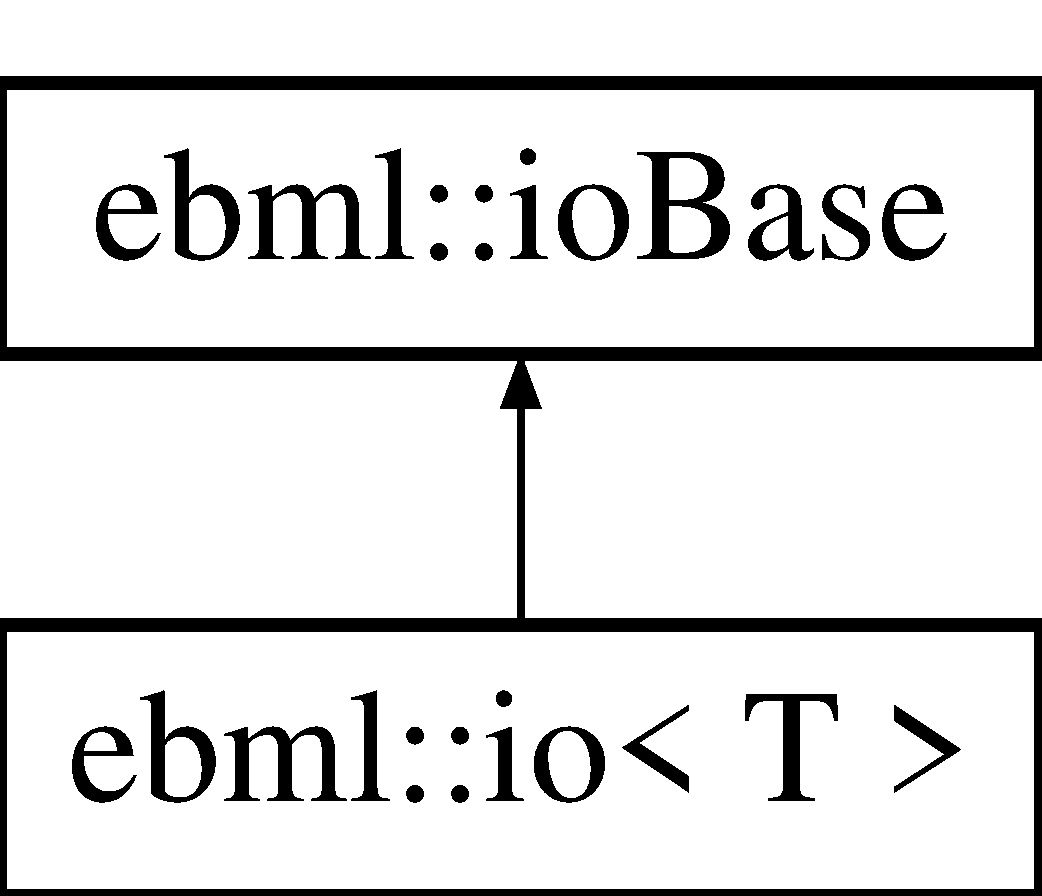
\includegraphics[height=2.000000cm]{classebml_1_1ioBase}
\end{center}
\end{figure}
\subsection*{Public Member Functions}
\begin{DoxyCompactItemize}
\item 
\mbox{\hyperlink{classebml_1_1ioBase_af0d31f731961fad7d3db80ba51a44ad1}{io\+Base}} ()
\item 
\mbox{\hyperlink{classebml_1_1ioBase_a97917f5c8816a035e3bc3f2e300da596}{$\sim$io\+Base}} ()
\item 
size\+\_\+t \mbox{\hyperlink{classebml_1_1ioBase_a3c2cd427ce1fd34a93959778a3fd4efa}{read}} (char $\ast$, size\+\_\+t)
\item 
size\+\_\+t \mbox{\hyperlink{classebml_1_1ioBase_a3895c5e0f86ecdcedaa288e87d68ccad}{write}} (const char $\ast$, size\+\_\+t)
\item 
off\+\_\+t \mbox{\hyperlink{classebml_1_1ioBase_ac4a5db64f2c7c8e791039f1b269d8f1a}{seek}} (off\+\_\+t, int whence=S\+E\+E\+K\+\_\+\+S\+ET)
\item 
virtual bool \mbox{\hyperlink{classebml_1_1ioBase_a413541f633f97d68021cbf58837e1970}{seekable}} ()=0
\item 
off\+\_\+t \mbox{\hyperlink{classebml_1_1ioBase_af0911dd01f1bb6a7ab284770c178db59}{tell}} ()
\item 
virtual size\+\_\+t \mbox{\hyperlink{classebml_1_1ioBase_aba93b64f19016207b3d6c43183a2be07}{read}} (char $\ast$, off\+\_\+t, size\+\_\+t)=0
\item 
virtual size\+\_\+t \mbox{\hyperlink{classebml_1_1ioBase_ad4a000de5db86375be0bf338130f76c9}{write}} (const char $\ast$, off\+\_\+t, size\+\_\+t)=0
\item 
void \mbox{\hyperlink{classebml_1_1ioBase_a802fbbe754413842f45251daa8294965}{close}} ()
\item 
bool \mbox{\hyperlink{classebml_1_1ioBase_a9dea7dea0e8d87a537e652e7f40128e9}{closed}} () const
\item 
virtual void \mbox{\hyperlink{classebml_1_1ioBase_a4cd6d91c2bb18a21c0fec425432b58c3}{truncate}} ()=0
\item 
virtual void \mbox{\hyperlink{classebml_1_1ioBase_ae1a40372ba926becab957ae0b054492e}{truncate}} (off\+\_\+t)=0
\item 
std\+::unique\+\_\+lock$<$ std\+::recursive\+\_\+mutex $>$ \mbox{\hyperlink{classebml_1_1ioBase_a8414aaadabbfdc746e810527bc76a93d}{acquire\+Lock}} ()
\end{DoxyCompactItemize}
\subsection*{Protected Member Functions}
\begin{DoxyCompactItemize}
\item 
virtual size\+\_\+t \mbox{\hyperlink{classebml_1_1ioBase_a00c5ba612f103ea06243d92f2410bc14}{\+\_\+read}} (char $\ast$, size\+\_\+t)=0
\item 
virtual size\+\_\+t \mbox{\hyperlink{classebml_1_1ioBase_a908cb3c7e36e440be2b3019e9e09a780}{\+\_\+write}} (const char $\ast$, size\+\_\+t)=0
\item 
virtual off\+\_\+t \mbox{\hyperlink{classebml_1_1ioBase_add69b836450d14e75580cec66ac04229}{\+\_\+seek}} (off\+\_\+t, int)=0
\item 
virtual off\+\_\+t \mbox{\hyperlink{classebml_1_1ioBase_a7cdde34fd8a6bb1968130e6e4cf74bc2}{\+\_\+tell}} ()=0
\item 
virtual void \mbox{\hyperlink{classebml_1_1ioBase_aaf78807501111b7351eb3ffaaeb3d9b8}{\+\_\+close}} ()=0
\item 
\mbox{\hyperlink{classebml_1_1ioBase_a51bc16ce542fdba5afca9ed711e89075}{io\+Base}} (const \mbox{\hyperlink{classebml_1_1ioBase}{io\+Base}} \&)
\item 
\mbox{\hyperlink{classebml_1_1ioBase}{io\+Base}} \& \mbox{\hyperlink{classebml_1_1ioBase_acdce9702e9511b87d0bea6b73b2fda5e}{operator=}} (const \mbox{\hyperlink{classebml_1_1ioBase}{io\+Base}} \&)
\end{DoxyCompactItemize}
\subsection*{Protected Attributes}
\begin{DoxyCompactItemize}
\item 
off\+\_\+t \mbox{\hyperlink{classebml_1_1ioBase_ada889242b80f658e0a80a465bf2bd9f7}{\+\_\+pos}}
\item 
bool \mbox{\hyperlink{classebml_1_1ioBase_ab87e105b03270d59019c05e7451b51d3}{\+\_\+closed}} = 0
\item 
bool \mbox{\hyperlink{classebml_1_1ioBase_a0083c31349d480a5e3b83dd366c22144}{\+\_\+close\+\_\+on\+\_\+dealloc}} = 0
\end{DoxyCompactItemize}


\subsection{Constructor \& Destructor Documentation}
\mbox{\Hypertarget{classebml_1_1ioBase_af0d31f731961fad7d3db80ba51a44ad1}\label{classebml_1_1ioBase_af0d31f731961fad7d3db80ba51a44ad1}} 
\index{ebml\+::io\+Base@{ebml\+::io\+Base}!io\+Base@{io\+Base}}
\index{io\+Base@{io\+Base}!ebml\+::io\+Base@{ebml\+::io\+Base}}
\subsubsection{\texorpdfstring{io\+Base()}{ioBase()}\hspace{0.1cm}{\footnotesize\ttfamily [1/2]}}
{\footnotesize\ttfamily ebml\+::io\+Base\+::io\+Base (\begin{DoxyParamCaption}{ }\end{DoxyParamCaption})\hspace{0.3cm}{\ttfamily [inline]}}

\mbox{\Hypertarget{classebml_1_1ioBase_a97917f5c8816a035e3bc3f2e300da596}\label{classebml_1_1ioBase_a97917f5c8816a035e3bc3f2e300da596}} 
\index{ebml\+::io\+Base@{ebml\+::io\+Base}!````~io\+Base@{$\sim$io\+Base}}
\index{````~io\+Base@{$\sim$io\+Base}!ebml\+::io\+Base@{ebml\+::io\+Base}}
\subsubsection{\texorpdfstring{$\sim$io\+Base()}{~ioBase()}}
{\footnotesize\ttfamily ebml\+::io\+Base\+::$\sim$io\+Base (\begin{DoxyParamCaption}{ }\end{DoxyParamCaption})}

\mbox{\Hypertarget{classebml_1_1ioBase_a51bc16ce542fdba5afca9ed711e89075}\label{classebml_1_1ioBase_a51bc16ce542fdba5afca9ed711e89075}} 
\index{ebml\+::io\+Base@{ebml\+::io\+Base}!io\+Base@{io\+Base}}
\index{io\+Base@{io\+Base}!ebml\+::io\+Base@{ebml\+::io\+Base}}
\subsubsection{\texorpdfstring{io\+Base()}{ioBase()}\hspace{0.1cm}{\footnotesize\ttfamily [2/2]}}
{\footnotesize\ttfamily ebml\+::io\+Base\+::io\+Base (\begin{DoxyParamCaption}\item[{const \mbox{\hyperlink{classebml_1_1ioBase}{io\+Base}} \&}]{ }\end{DoxyParamCaption})\hspace{0.3cm}{\ttfamily [protected]}}



\subsection{Member Function Documentation}
\mbox{\Hypertarget{classebml_1_1ioBase_aaf78807501111b7351eb3ffaaeb3d9b8}\label{classebml_1_1ioBase_aaf78807501111b7351eb3ffaaeb3d9b8}} 
\index{ebml\+::io\+Base@{ebml\+::io\+Base}!\+\_\+close@{\+\_\+close}}
\index{\+\_\+close@{\+\_\+close}!ebml\+::io\+Base@{ebml\+::io\+Base}}
\subsubsection{\texorpdfstring{\+\_\+close()}{\_close()}}
{\footnotesize\ttfamily virtual void ebml\+::io\+Base\+::\+\_\+close (\begin{DoxyParamCaption}{ }\end{DoxyParamCaption})\hspace{0.3cm}{\ttfamily [protected]}, {\ttfamily [pure virtual]}}

\mbox{\Hypertarget{classebml_1_1ioBase_a00c5ba612f103ea06243d92f2410bc14}\label{classebml_1_1ioBase_a00c5ba612f103ea06243d92f2410bc14}} 
\index{ebml\+::io\+Base@{ebml\+::io\+Base}!\+\_\+read@{\+\_\+read}}
\index{\+\_\+read@{\+\_\+read}!ebml\+::io\+Base@{ebml\+::io\+Base}}
\subsubsection{\texorpdfstring{\+\_\+read()}{\_read()}}
{\footnotesize\ttfamily virtual size\+\_\+t ebml\+::io\+Base\+::\+\_\+read (\begin{DoxyParamCaption}\item[{char $\ast$}]{,  }\item[{size\+\_\+t}]{ }\end{DoxyParamCaption})\hspace{0.3cm}{\ttfamily [protected]}, {\ttfamily [pure virtual]}}

\mbox{\Hypertarget{classebml_1_1ioBase_add69b836450d14e75580cec66ac04229}\label{classebml_1_1ioBase_add69b836450d14e75580cec66ac04229}} 
\index{ebml\+::io\+Base@{ebml\+::io\+Base}!\+\_\+seek@{\+\_\+seek}}
\index{\+\_\+seek@{\+\_\+seek}!ebml\+::io\+Base@{ebml\+::io\+Base}}
\subsubsection{\texorpdfstring{\+\_\+seek()}{\_seek()}}
{\footnotesize\ttfamily virtual off\+\_\+t ebml\+::io\+Base\+::\+\_\+seek (\begin{DoxyParamCaption}\item[{off\+\_\+t}]{,  }\item[{int}]{ }\end{DoxyParamCaption})\hspace{0.3cm}{\ttfamily [protected]}, {\ttfamily [pure virtual]}}

\mbox{\Hypertarget{classebml_1_1ioBase_a7cdde34fd8a6bb1968130e6e4cf74bc2}\label{classebml_1_1ioBase_a7cdde34fd8a6bb1968130e6e4cf74bc2}} 
\index{ebml\+::io\+Base@{ebml\+::io\+Base}!\+\_\+tell@{\+\_\+tell}}
\index{\+\_\+tell@{\+\_\+tell}!ebml\+::io\+Base@{ebml\+::io\+Base}}
\subsubsection{\texorpdfstring{\+\_\+tell()}{\_tell()}}
{\footnotesize\ttfamily virtual off\+\_\+t ebml\+::io\+Base\+::\+\_\+tell (\begin{DoxyParamCaption}{ }\end{DoxyParamCaption})\hspace{0.3cm}{\ttfamily [protected]}, {\ttfamily [pure virtual]}}

\mbox{\Hypertarget{classebml_1_1ioBase_a908cb3c7e36e440be2b3019e9e09a780}\label{classebml_1_1ioBase_a908cb3c7e36e440be2b3019e9e09a780}} 
\index{ebml\+::io\+Base@{ebml\+::io\+Base}!\+\_\+write@{\+\_\+write}}
\index{\+\_\+write@{\+\_\+write}!ebml\+::io\+Base@{ebml\+::io\+Base}}
\subsubsection{\texorpdfstring{\+\_\+write()}{\_write()}}
{\footnotesize\ttfamily virtual size\+\_\+t ebml\+::io\+Base\+::\+\_\+write (\begin{DoxyParamCaption}\item[{const char $\ast$}]{,  }\item[{size\+\_\+t}]{ }\end{DoxyParamCaption})\hspace{0.3cm}{\ttfamily [protected]}, {\ttfamily [pure virtual]}}

\mbox{\Hypertarget{classebml_1_1ioBase_a8414aaadabbfdc746e810527bc76a93d}\label{classebml_1_1ioBase_a8414aaadabbfdc746e810527bc76a93d}} 
\index{ebml\+::io\+Base@{ebml\+::io\+Base}!acquire\+Lock@{acquire\+Lock}}
\index{acquire\+Lock@{acquire\+Lock}!ebml\+::io\+Base@{ebml\+::io\+Base}}
\subsubsection{\texorpdfstring{acquire\+Lock()}{acquireLock()}}
{\footnotesize\ttfamily std\+::unique\+\_\+lock$<$std\+::recursive\+\_\+mutex$>$ ebml\+::io\+Base\+::acquire\+Lock (\begin{DoxyParamCaption}{ }\end{DoxyParamCaption})\hspace{0.3cm}{\ttfamily [inline]}}

\mbox{\Hypertarget{classebml_1_1ioBase_a802fbbe754413842f45251daa8294965}\label{classebml_1_1ioBase_a802fbbe754413842f45251daa8294965}} 
\index{ebml\+::io\+Base@{ebml\+::io\+Base}!close@{close}}
\index{close@{close}!ebml\+::io\+Base@{ebml\+::io\+Base}}
\subsubsection{\texorpdfstring{close()}{close()}}
{\footnotesize\ttfamily void ebml\+::io\+Base\+::close (\begin{DoxyParamCaption}{ }\end{DoxyParamCaption})}

\mbox{\Hypertarget{classebml_1_1ioBase_a9dea7dea0e8d87a537e652e7f40128e9}\label{classebml_1_1ioBase_a9dea7dea0e8d87a537e652e7f40128e9}} 
\index{ebml\+::io\+Base@{ebml\+::io\+Base}!closed@{closed}}
\index{closed@{closed}!ebml\+::io\+Base@{ebml\+::io\+Base}}
\subsubsection{\texorpdfstring{closed()}{closed()}}
{\footnotesize\ttfamily bool ebml\+::io\+Base\+::closed (\begin{DoxyParamCaption}{ }\end{DoxyParamCaption}) const}

\mbox{\Hypertarget{classebml_1_1ioBase_acdce9702e9511b87d0bea6b73b2fda5e}\label{classebml_1_1ioBase_acdce9702e9511b87d0bea6b73b2fda5e}} 
\index{ebml\+::io\+Base@{ebml\+::io\+Base}!operator=@{operator=}}
\index{operator=@{operator=}!ebml\+::io\+Base@{ebml\+::io\+Base}}
\subsubsection{\texorpdfstring{operator=()}{operator=()}}
{\footnotesize\ttfamily \mbox{\hyperlink{classebml_1_1ioBase}{io\+Base}}\& ebml\+::io\+Base\+::operator= (\begin{DoxyParamCaption}\item[{const \mbox{\hyperlink{classebml_1_1ioBase}{io\+Base}} \&}]{ }\end{DoxyParamCaption})\hspace{0.3cm}{\ttfamily [protected]}}

\mbox{\Hypertarget{classebml_1_1ioBase_a3c2cd427ce1fd34a93959778a3fd4efa}\label{classebml_1_1ioBase_a3c2cd427ce1fd34a93959778a3fd4efa}} 
\index{ebml\+::io\+Base@{ebml\+::io\+Base}!read@{read}}
\index{read@{read}!ebml\+::io\+Base@{ebml\+::io\+Base}}
\subsubsection{\texorpdfstring{read()}{read()}\hspace{0.1cm}{\footnotesize\ttfamily [1/2]}}
{\footnotesize\ttfamily size\+\_\+t ebml\+::io\+Base\+::read (\begin{DoxyParamCaption}\item[{char $\ast$}]{,  }\item[{size\+\_\+t}]{ }\end{DoxyParamCaption})}

\mbox{\Hypertarget{classebml_1_1ioBase_aba93b64f19016207b3d6c43183a2be07}\label{classebml_1_1ioBase_aba93b64f19016207b3d6c43183a2be07}} 
\index{ebml\+::io\+Base@{ebml\+::io\+Base}!read@{read}}
\index{read@{read}!ebml\+::io\+Base@{ebml\+::io\+Base}}
\subsubsection{\texorpdfstring{read()}{read()}\hspace{0.1cm}{\footnotesize\ttfamily [2/2]}}
{\footnotesize\ttfamily virtual size\+\_\+t ebml\+::io\+Base\+::read (\begin{DoxyParamCaption}\item[{char $\ast$}]{,  }\item[{off\+\_\+t}]{,  }\item[{size\+\_\+t}]{ }\end{DoxyParamCaption})\hspace{0.3cm}{\ttfamily [pure virtual]}}



Implemented in \mbox{\hyperlink{classebml_1_1io_ad745dc2c29544750dcd38a21cba0a16c}{ebml\+::io$<$ T $>$}}, and \mbox{\hyperlink{classebml_1_1io_a3b291aa8fb7bbeeb3f9d2ef152c37115}{ebml\+::io$<$ T $>$}}.

\mbox{\Hypertarget{classebml_1_1ioBase_ac4a5db64f2c7c8e791039f1b269d8f1a}\label{classebml_1_1ioBase_ac4a5db64f2c7c8e791039f1b269d8f1a}} 
\index{ebml\+::io\+Base@{ebml\+::io\+Base}!seek@{seek}}
\index{seek@{seek}!ebml\+::io\+Base@{ebml\+::io\+Base}}
\subsubsection{\texorpdfstring{seek()}{seek()}}
{\footnotesize\ttfamily off\+\_\+t ebml\+::io\+Base\+::seek (\begin{DoxyParamCaption}\item[{off\+\_\+t}]{,  }\item[{int}]{whence = {\ttfamily SEEK\+\_\+SET} }\end{DoxyParamCaption})}

\mbox{\Hypertarget{classebml_1_1ioBase_a413541f633f97d68021cbf58837e1970}\label{classebml_1_1ioBase_a413541f633f97d68021cbf58837e1970}} 
\index{ebml\+::io\+Base@{ebml\+::io\+Base}!seekable@{seekable}}
\index{seekable@{seekable}!ebml\+::io\+Base@{ebml\+::io\+Base}}
\subsubsection{\texorpdfstring{seekable()}{seekable()}}
{\footnotesize\ttfamily virtual bool ebml\+::io\+Base\+::seekable (\begin{DoxyParamCaption}{ }\end{DoxyParamCaption})\hspace{0.3cm}{\ttfamily [pure virtual]}}



Implemented in \mbox{\hyperlink{classebml_1_1io_ab019a4128b3339941124a12632c919fd}{ebml\+::io$<$ T $>$}}, \mbox{\hyperlink{classebml_1_1io_a4ea6caf18c5646646b3a15bc3c59a5ab}{ebml\+::io$<$ T $>$}}, and \mbox{\hyperlink{classebml_1_1io_a6e97c1e6868bf65286328b9447eaa419}{ebml\+::io$<$ T $>$}}.

\mbox{\Hypertarget{classebml_1_1ioBase_af0911dd01f1bb6a7ab284770c178db59}\label{classebml_1_1ioBase_af0911dd01f1bb6a7ab284770c178db59}} 
\index{ebml\+::io\+Base@{ebml\+::io\+Base}!tell@{tell}}
\index{tell@{tell}!ebml\+::io\+Base@{ebml\+::io\+Base}}
\subsubsection{\texorpdfstring{tell()}{tell()}}
{\footnotesize\ttfamily off\+\_\+t ebml\+::io\+Base\+::tell (\begin{DoxyParamCaption}{ }\end{DoxyParamCaption})}

\mbox{\Hypertarget{classebml_1_1ioBase_a4cd6d91c2bb18a21c0fec425432b58c3}\label{classebml_1_1ioBase_a4cd6d91c2bb18a21c0fec425432b58c3}} 
\index{ebml\+::io\+Base@{ebml\+::io\+Base}!truncate@{truncate}}
\index{truncate@{truncate}!ebml\+::io\+Base@{ebml\+::io\+Base}}
\subsubsection{\texorpdfstring{truncate()}{truncate()}\hspace{0.1cm}{\footnotesize\ttfamily [1/2]}}
{\footnotesize\ttfamily virtual void ebml\+::io\+Base\+::truncate (\begin{DoxyParamCaption}{ }\end{DoxyParamCaption})\hspace{0.3cm}{\ttfamily [pure virtual]}}



Implemented in \mbox{\hyperlink{classebml_1_1io_a6a5c0f2182844094c6b4432a15adccc8}{ebml\+::io$<$ T $>$}}.

\mbox{\Hypertarget{classebml_1_1ioBase_ae1a40372ba926becab957ae0b054492e}\label{classebml_1_1ioBase_ae1a40372ba926becab957ae0b054492e}} 
\index{ebml\+::io\+Base@{ebml\+::io\+Base}!truncate@{truncate}}
\index{truncate@{truncate}!ebml\+::io\+Base@{ebml\+::io\+Base}}
\subsubsection{\texorpdfstring{truncate()}{truncate()}\hspace{0.1cm}{\footnotesize\ttfamily [2/2]}}
{\footnotesize\ttfamily virtual void ebml\+::io\+Base\+::truncate (\begin{DoxyParamCaption}\item[{off\+\_\+t}]{ }\end{DoxyParamCaption})\hspace{0.3cm}{\ttfamily [pure virtual]}}



Implemented in \mbox{\hyperlink{classebml_1_1io_a9a50a99136e7e9a4a404dc3087024a7f}{ebml\+::io$<$ T $>$}}.

\mbox{\Hypertarget{classebml_1_1ioBase_a3895c5e0f86ecdcedaa288e87d68ccad}\label{classebml_1_1ioBase_a3895c5e0f86ecdcedaa288e87d68ccad}} 
\index{ebml\+::io\+Base@{ebml\+::io\+Base}!write@{write}}
\index{write@{write}!ebml\+::io\+Base@{ebml\+::io\+Base}}
\subsubsection{\texorpdfstring{write()}{write()}\hspace{0.1cm}{\footnotesize\ttfamily [1/2]}}
{\footnotesize\ttfamily size\+\_\+t ebml\+::io\+Base\+::write (\begin{DoxyParamCaption}\item[{const char $\ast$}]{,  }\item[{size\+\_\+t}]{ }\end{DoxyParamCaption})}

\mbox{\Hypertarget{classebml_1_1ioBase_ad4a000de5db86375be0bf338130f76c9}\label{classebml_1_1ioBase_ad4a000de5db86375be0bf338130f76c9}} 
\index{ebml\+::io\+Base@{ebml\+::io\+Base}!write@{write}}
\index{write@{write}!ebml\+::io\+Base@{ebml\+::io\+Base}}
\subsubsection{\texorpdfstring{write()}{write()}\hspace{0.1cm}{\footnotesize\ttfamily [2/2]}}
{\footnotesize\ttfamily virtual size\+\_\+t ebml\+::io\+Base\+::write (\begin{DoxyParamCaption}\item[{const char $\ast$}]{,  }\item[{off\+\_\+t}]{,  }\item[{size\+\_\+t}]{ }\end{DoxyParamCaption})\hspace{0.3cm}{\ttfamily [pure virtual]}}



Implemented in \mbox{\hyperlink{classebml_1_1io_a5c3f2df6edfbd090b4d0fbc8a6dacccb}{ebml\+::io$<$ T $>$}}, and \mbox{\hyperlink{classebml_1_1io_aedbdf5a69ee0ae64f909a59645cd0db7}{ebml\+::io$<$ T $>$}}.



\subsection{Member Data Documentation}
\mbox{\Hypertarget{classebml_1_1ioBase_a0083c31349d480a5e3b83dd366c22144}\label{classebml_1_1ioBase_a0083c31349d480a5e3b83dd366c22144}} 
\index{ebml\+::io\+Base@{ebml\+::io\+Base}!\+\_\+close\+\_\+on\+\_\+dealloc@{\+\_\+close\+\_\+on\+\_\+dealloc}}
\index{\+\_\+close\+\_\+on\+\_\+dealloc@{\+\_\+close\+\_\+on\+\_\+dealloc}!ebml\+::io\+Base@{ebml\+::io\+Base}}
\subsubsection{\texorpdfstring{\+\_\+close\+\_\+on\+\_\+dealloc}{\_close\_on\_dealloc}}
{\footnotesize\ttfamily bool ebml\+::io\+Base\+::\+\_\+close\+\_\+on\+\_\+dealloc = 0\hspace{0.3cm}{\ttfamily [protected]}}

\mbox{\Hypertarget{classebml_1_1ioBase_ab87e105b03270d59019c05e7451b51d3}\label{classebml_1_1ioBase_ab87e105b03270d59019c05e7451b51d3}} 
\index{ebml\+::io\+Base@{ebml\+::io\+Base}!\+\_\+closed@{\+\_\+closed}}
\index{\+\_\+closed@{\+\_\+closed}!ebml\+::io\+Base@{ebml\+::io\+Base}}
\subsubsection{\texorpdfstring{\+\_\+closed}{\_closed}}
{\footnotesize\ttfamily bool ebml\+::io\+Base\+::\+\_\+closed = 0\hspace{0.3cm}{\ttfamily [protected]}}

\mbox{\Hypertarget{classebml_1_1ioBase_ada889242b80f658e0a80a465bf2bd9f7}\label{classebml_1_1ioBase_ada889242b80f658e0a80a465bf2bd9f7}} 
\index{ebml\+::io\+Base@{ebml\+::io\+Base}!\+\_\+pos@{\+\_\+pos}}
\index{\+\_\+pos@{\+\_\+pos}!ebml\+::io\+Base@{ebml\+::io\+Base}}
\subsubsection{\texorpdfstring{\+\_\+pos}{\_pos}}
{\footnotesize\ttfamily off\+\_\+t ebml\+::io\+Base\+::\+\_\+pos\hspace{0.3cm}{\ttfamily [protected]}}



The documentation for this class was generated from the following file\+:\begin{DoxyCompactItemize}
\item 
include/libebml\+\_\+ng/\mbox{\hyperlink{io_8h}{io.\+h}}\end{DoxyCompactItemize}

\hypertarget{classebml_1_1ebmlMasterElement_1_1iterator}{}\section{ebml\+:\+:ebml\+Master\+Element\+:\+:iterator Class Reference}
\label{classebml_1_1ebmlMasterElement_1_1iterator}\index{ebml\+::ebml\+Master\+Element\+::iterator@{ebml\+::ebml\+Master\+Element\+::iterator}}


{\ttfamily \#include $<$base.\+h$>$}

\subsection*{Public Member Functions}
\begin{DoxyCompactItemize}
\item 
const \mbox{\hyperlink{namespaceebml_adad533b7705a16bb360fe56380c5e7be}{ebml\+Element\+\_\+sp}} \& \mbox{\hyperlink{classebml_1_1ebmlMasterElement_1_1iterator_ad6c25c2646a81bd03948ca61f768af68}{operator$\ast$}} () const
\item 
\mbox{\hyperlink{classebml_1_1ebmlMasterElement_1_1iterator}{iterator}} \& \mbox{\hyperlink{classebml_1_1ebmlMasterElement_1_1iterator_a92ad796c55701c667c114ac54dc5004f}{operator++}} ()
\item 
\mbox{\hyperlink{classebml_1_1ebmlMasterElement_1_1iterator_aff65b96ef2b667cd5044d594da574d79}{iterator}} (const \mbox{\hyperlink{classebml_1_1ebmlMasterElement_1_1iterator}{iterator}} \&)
\item 
\mbox{\hyperlink{classebml_1_1ebmlMasterElement_1_1iterator_a36ed970a665ddd45cadee9dee281d334}{iterator}} (\mbox{\hyperlink{classebml_1_1ebmlMasterElement_1_1iterator}{iterator}} \&\&)
\item 
\mbox{\hyperlink{classebml_1_1ebmlMasterElement_1_1iterator}{iterator}} \& \mbox{\hyperlink{classebml_1_1ebmlMasterElement_1_1iterator_a162e7b8f1e830065d05b632314afb28a}{operator=}} (const \mbox{\hyperlink{classebml_1_1ebmlMasterElement_1_1iterator}{iterator}} \&)
\item 
\mbox{\hyperlink{classebml_1_1ebmlMasterElement_1_1iterator}{iterator}} \& \mbox{\hyperlink{classebml_1_1ebmlMasterElement_1_1iterator_a91f28b49e638ea9fa9c5ea5a6807e567}{operator=}} (\mbox{\hyperlink{classebml_1_1ebmlMasterElement_1_1iterator}{iterator}} \&\&)
\item 
bool \mbox{\hyperlink{classebml_1_1ebmlMasterElement_1_1iterator_afb3fe9d5db619b912eec528d2b2d71c5}{operator==}} (const \mbox{\hyperlink{classebml_1_1ebmlMasterElement_1_1iterator}{iterator}} \&) const
\item 
bool \mbox{\hyperlink{classebml_1_1ebmlMasterElement_1_1iterator_a61dc214c93030ee9749e760aa1b4b112}{operator!=}} (const \mbox{\hyperlink{classebml_1_1ebmlMasterElement_1_1iterator}{iterator}} \&) const
\item 
\mbox{\hyperlink{classebml_1_1ebmlMasterElement_1_1iterator_a0f90808779c8545321c75488c8027e20}{$\sim$iterator}} ()
\end{DoxyCompactItemize}
\subsection*{Protected Member Functions}
\begin{DoxyCompactItemize}
\item 
\mbox{\hyperlink{classebml_1_1ebmlMasterElement_1_1iterator_af3851f8e35252a05f89d55f76fb40e7d}{iterator}} (\mbox{\hyperlink{classebml_1_1ebmlMasterElement_1_1__iterator}{\+\_\+iterator}} $\ast$)
\end{DoxyCompactItemize}
\subsection*{Friends}
\begin{DoxyCompactItemize}
\item 
class \mbox{\hyperlink{classebml_1_1ebmlMasterElement_1_1iterator_ad88e86cba72e9332a4693c1c6009b281}{ebml\+Master\+Element}}
\end{DoxyCompactItemize}


\subsection{Constructor \& Destructor Documentation}
\mbox{\Hypertarget{classebml_1_1ebmlMasterElement_1_1iterator_af3851f8e35252a05f89d55f76fb40e7d}\label{classebml_1_1ebmlMasterElement_1_1iterator_af3851f8e35252a05f89d55f76fb40e7d}} 
\index{ebml\+::ebml\+Master\+Element\+::iterator@{ebml\+::ebml\+Master\+Element\+::iterator}!iterator@{iterator}}
\index{iterator@{iterator}!ebml\+::ebml\+Master\+Element\+::iterator@{ebml\+::ebml\+Master\+Element\+::iterator}}
\subsubsection{\texorpdfstring{iterator()}{iterator()}\hspace{0.1cm}{\footnotesize\ttfamily [1/3]}}
{\footnotesize\ttfamily ebml\+::ebml\+Master\+Element\+::iterator\+::iterator (\begin{DoxyParamCaption}\item[{\mbox{\hyperlink{classebml_1_1ebmlMasterElement_1_1__iterator}{\+\_\+iterator}} $\ast$}]{ }\end{DoxyParamCaption})\hspace{0.3cm}{\ttfamily [protected]}}

\mbox{\Hypertarget{classebml_1_1ebmlMasterElement_1_1iterator_aff65b96ef2b667cd5044d594da574d79}\label{classebml_1_1ebmlMasterElement_1_1iterator_aff65b96ef2b667cd5044d594da574d79}} 
\index{ebml\+::ebml\+Master\+Element\+::iterator@{ebml\+::ebml\+Master\+Element\+::iterator}!iterator@{iterator}}
\index{iterator@{iterator}!ebml\+::ebml\+Master\+Element\+::iterator@{ebml\+::ebml\+Master\+Element\+::iterator}}
\subsubsection{\texorpdfstring{iterator()}{iterator()}\hspace{0.1cm}{\footnotesize\ttfamily [2/3]}}
{\footnotesize\ttfamily ebml\+::ebml\+Master\+Element\+::iterator\+::iterator (\begin{DoxyParamCaption}\item[{const \mbox{\hyperlink{classebml_1_1ebmlMasterElement_1_1iterator}{iterator}} \&}]{ }\end{DoxyParamCaption})}

\mbox{\Hypertarget{classebml_1_1ebmlMasterElement_1_1iterator_a36ed970a665ddd45cadee9dee281d334}\label{classebml_1_1ebmlMasterElement_1_1iterator_a36ed970a665ddd45cadee9dee281d334}} 
\index{ebml\+::ebml\+Master\+Element\+::iterator@{ebml\+::ebml\+Master\+Element\+::iterator}!iterator@{iterator}}
\index{iterator@{iterator}!ebml\+::ebml\+Master\+Element\+::iterator@{ebml\+::ebml\+Master\+Element\+::iterator}}
\subsubsection{\texorpdfstring{iterator()}{iterator()}\hspace{0.1cm}{\footnotesize\ttfamily [3/3]}}
{\footnotesize\ttfamily ebml\+::ebml\+Master\+Element\+::iterator\+::iterator (\begin{DoxyParamCaption}\item[{\mbox{\hyperlink{classebml_1_1ebmlMasterElement_1_1iterator}{iterator}} \&\&}]{ }\end{DoxyParamCaption})}

\mbox{\Hypertarget{classebml_1_1ebmlMasterElement_1_1iterator_a0f90808779c8545321c75488c8027e20}\label{classebml_1_1ebmlMasterElement_1_1iterator_a0f90808779c8545321c75488c8027e20}} 
\index{ebml\+::ebml\+Master\+Element\+::iterator@{ebml\+::ebml\+Master\+Element\+::iterator}!````~iterator@{$\sim$iterator}}
\index{````~iterator@{$\sim$iterator}!ebml\+::ebml\+Master\+Element\+::iterator@{ebml\+::ebml\+Master\+Element\+::iterator}}
\subsubsection{\texorpdfstring{$\sim$iterator()}{~iterator()}}
{\footnotesize\ttfamily ebml\+::ebml\+Master\+Element\+::iterator\+::$\sim$iterator (\begin{DoxyParamCaption}{ }\end{DoxyParamCaption})}



\subsection{Member Function Documentation}
\mbox{\Hypertarget{classebml_1_1ebmlMasterElement_1_1iterator_a61dc214c93030ee9749e760aa1b4b112}\label{classebml_1_1ebmlMasterElement_1_1iterator_a61dc214c93030ee9749e760aa1b4b112}} 
\index{ebml\+::ebml\+Master\+Element\+::iterator@{ebml\+::ebml\+Master\+Element\+::iterator}!operator"!=@{operator"!=}}
\index{operator"!=@{operator"!=}!ebml\+::ebml\+Master\+Element\+::iterator@{ebml\+::ebml\+Master\+Element\+::iterator}}
\subsubsection{\texorpdfstring{operator"!=()}{operator!=()}}
{\footnotesize\ttfamily bool ebml\+::ebml\+Master\+Element\+::iterator\+::operator!= (\begin{DoxyParamCaption}\item[{const \mbox{\hyperlink{classebml_1_1ebmlMasterElement_1_1iterator}{iterator}} \&}]{ }\end{DoxyParamCaption}) const}

\mbox{\Hypertarget{classebml_1_1ebmlMasterElement_1_1iterator_ad6c25c2646a81bd03948ca61f768af68}\label{classebml_1_1ebmlMasterElement_1_1iterator_ad6c25c2646a81bd03948ca61f768af68}} 
\index{ebml\+::ebml\+Master\+Element\+::iterator@{ebml\+::ebml\+Master\+Element\+::iterator}!operator$\ast$@{operator$\ast$}}
\index{operator$\ast$@{operator$\ast$}!ebml\+::ebml\+Master\+Element\+::iterator@{ebml\+::ebml\+Master\+Element\+::iterator}}
\subsubsection{\texorpdfstring{operator$\ast$()}{operator*()}}
{\footnotesize\ttfamily const \mbox{\hyperlink{namespaceebml_adad533b7705a16bb360fe56380c5e7be}{ebml\+Element\+\_\+sp}}\& ebml\+::ebml\+Master\+Element\+::iterator\+::operator$\ast$ (\begin{DoxyParamCaption}{ }\end{DoxyParamCaption}) const}

\mbox{\Hypertarget{classebml_1_1ebmlMasterElement_1_1iterator_a92ad796c55701c667c114ac54dc5004f}\label{classebml_1_1ebmlMasterElement_1_1iterator_a92ad796c55701c667c114ac54dc5004f}} 
\index{ebml\+::ebml\+Master\+Element\+::iterator@{ebml\+::ebml\+Master\+Element\+::iterator}!operator++@{operator++}}
\index{operator++@{operator++}!ebml\+::ebml\+Master\+Element\+::iterator@{ebml\+::ebml\+Master\+Element\+::iterator}}
\subsubsection{\texorpdfstring{operator++()}{operator++()}}
{\footnotesize\ttfamily \mbox{\hyperlink{classebml_1_1ebmlMasterElement_1_1iterator}{iterator}}\& ebml\+::ebml\+Master\+Element\+::iterator\+::operator++ (\begin{DoxyParamCaption}{ }\end{DoxyParamCaption})}

\mbox{\Hypertarget{classebml_1_1ebmlMasterElement_1_1iterator_a162e7b8f1e830065d05b632314afb28a}\label{classebml_1_1ebmlMasterElement_1_1iterator_a162e7b8f1e830065d05b632314afb28a}} 
\index{ebml\+::ebml\+Master\+Element\+::iterator@{ebml\+::ebml\+Master\+Element\+::iterator}!operator=@{operator=}}
\index{operator=@{operator=}!ebml\+::ebml\+Master\+Element\+::iterator@{ebml\+::ebml\+Master\+Element\+::iterator}}
\subsubsection{\texorpdfstring{operator=()}{operator=()}\hspace{0.1cm}{\footnotesize\ttfamily [1/2]}}
{\footnotesize\ttfamily \mbox{\hyperlink{classebml_1_1ebmlMasterElement_1_1iterator}{iterator}}\& ebml\+::ebml\+Master\+Element\+::iterator\+::operator= (\begin{DoxyParamCaption}\item[{const \mbox{\hyperlink{classebml_1_1ebmlMasterElement_1_1iterator}{iterator}} \&}]{ }\end{DoxyParamCaption})}

\mbox{\Hypertarget{classebml_1_1ebmlMasterElement_1_1iterator_a91f28b49e638ea9fa9c5ea5a6807e567}\label{classebml_1_1ebmlMasterElement_1_1iterator_a91f28b49e638ea9fa9c5ea5a6807e567}} 
\index{ebml\+::ebml\+Master\+Element\+::iterator@{ebml\+::ebml\+Master\+Element\+::iterator}!operator=@{operator=}}
\index{operator=@{operator=}!ebml\+::ebml\+Master\+Element\+::iterator@{ebml\+::ebml\+Master\+Element\+::iterator}}
\subsubsection{\texorpdfstring{operator=()}{operator=()}\hspace{0.1cm}{\footnotesize\ttfamily [2/2]}}
{\footnotesize\ttfamily \mbox{\hyperlink{classebml_1_1ebmlMasterElement_1_1iterator}{iterator}}\& ebml\+::ebml\+Master\+Element\+::iterator\+::operator= (\begin{DoxyParamCaption}\item[{\mbox{\hyperlink{classebml_1_1ebmlMasterElement_1_1iterator}{iterator}} \&\&}]{ }\end{DoxyParamCaption})}

\mbox{\Hypertarget{classebml_1_1ebmlMasterElement_1_1iterator_afb3fe9d5db619b912eec528d2b2d71c5}\label{classebml_1_1ebmlMasterElement_1_1iterator_afb3fe9d5db619b912eec528d2b2d71c5}} 
\index{ebml\+::ebml\+Master\+Element\+::iterator@{ebml\+::ebml\+Master\+Element\+::iterator}!operator==@{operator==}}
\index{operator==@{operator==}!ebml\+::ebml\+Master\+Element\+::iterator@{ebml\+::ebml\+Master\+Element\+::iterator}}
\subsubsection{\texorpdfstring{operator==()}{operator==()}}
{\footnotesize\ttfamily bool ebml\+::ebml\+Master\+Element\+::iterator\+::operator== (\begin{DoxyParamCaption}\item[{const \mbox{\hyperlink{classebml_1_1ebmlMasterElement_1_1iterator}{iterator}} \&}]{ }\end{DoxyParamCaption}) const}



\subsection{Friends And Related Function Documentation}
\mbox{\Hypertarget{classebml_1_1ebmlMasterElement_1_1iterator_ad88e86cba72e9332a4693c1c6009b281}\label{classebml_1_1ebmlMasterElement_1_1iterator_ad88e86cba72e9332a4693c1c6009b281}} 
\index{ebml\+::ebml\+Master\+Element\+::iterator@{ebml\+::ebml\+Master\+Element\+::iterator}!ebml\+Master\+Element@{ebml\+Master\+Element}}
\index{ebml\+Master\+Element@{ebml\+Master\+Element}!ebml\+::ebml\+Master\+Element\+::iterator@{ebml\+::ebml\+Master\+Element\+::iterator}}
\subsubsection{\texorpdfstring{ebml\+Master\+Element}{ebmlMasterElement}}
{\footnotesize\ttfamily friend class \mbox{\hyperlink{classebml_1_1ebmlMasterElement}{ebml\+Master\+Element}}\hspace{0.3cm}{\ttfamily [friend]}}



The documentation for this class was generated from the following file\+:\begin{DoxyCompactItemize}
\item 
include/libebml\+\_\+ng/masterelement/\mbox{\hyperlink{masterelement_2base_8h}{base.\+h}}\end{DoxyCompactItemize}

\hypertarget{classebml_1_1parseString_1_1iterator}{}\section{ebml\+:\+:parse\+String\+:\+:iterator Class Reference}
\label{classebml_1_1parseString_1_1iterator}\index{ebml\+::parse\+String\+::iterator@{ebml\+::parse\+String\+::iterator}}


{\ttfamily \#include $<$string.\+h$>$}

\subsection*{Public Member Functions}
\begin{DoxyCompactItemize}
\item 
\mbox{\hyperlink{classebml_1_1parseString_1_1iterator_ab73280633b366afd2a53b689610585d9}{iterator}} (const char $\ast$, size\+\_\+t)
\item 
\mbox{\hyperlink{classebml_1_1parseString}{parse\+String}} \mbox{\hyperlink{classebml_1_1parseString_1_1iterator_abe2e504da9045240539efe00476f3bd0}{operator$\ast$}} ()
\item 
\mbox{\hyperlink{classebml_1_1parseString_1_1iterator}{parse\+String\+::iterator}} \& \mbox{\hyperlink{classebml_1_1parseString_1_1iterator_a289693cc2c25e4f0e24fbe51d0d59736}{operator++}} ()
\item 
\mbox{\hyperlink{classebml_1_1parseString_1_1iterator}{parse\+String\+::iterator}} \mbox{\hyperlink{classebml_1_1parseString_1_1iterator_a23a43b9b25bc3c9246aee8c89eac3f71}{operator++}} (int)
\item 
bool \mbox{\hyperlink{classebml_1_1parseString_1_1iterator_a6dd6eff768ec3385b2981d6861834056}{operator==}} (const \mbox{\hyperlink{classebml_1_1parseString_1_1iterator}{parse\+String\+::iterator}} \&) const
\item 
bool \mbox{\hyperlink{classebml_1_1parseString_1_1iterator_a2f93ead5c4fd4b6a84a269ba49432c4c}{operator!=}} (const \mbox{\hyperlink{classebml_1_1parseString_1_1iterator}{parse\+String\+::iterator}} \&) const
\item 
bool \mbox{\hyperlink{classebml_1_1parseString_1_1iterator_a9f929d744bd65be4508ac9403ed1f998}{at\+End}} () const
\end{DoxyCompactItemize}


\subsection{Constructor \& Destructor Documentation}
\mbox{\Hypertarget{classebml_1_1parseString_1_1iterator_ab73280633b366afd2a53b689610585d9}\label{classebml_1_1parseString_1_1iterator_ab73280633b366afd2a53b689610585d9}} 
\index{ebml\+::parse\+String\+::iterator@{ebml\+::parse\+String\+::iterator}!iterator@{iterator}}
\index{iterator@{iterator}!ebml\+::parse\+String\+::iterator@{ebml\+::parse\+String\+::iterator}}
\subsubsection{\texorpdfstring{iterator()}{iterator()}}
{\footnotesize\ttfamily ebml\+::parse\+String\+::iterator\+::iterator (\begin{DoxyParamCaption}\item[{const char $\ast$}]{,  }\item[{size\+\_\+t}]{ }\end{DoxyParamCaption})}



\subsection{Member Function Documentation}
\mbox{\Hypertarget{classebml_1_1parseString_1_1iterator_a9f929d744bd65be4508ac9403ed1f998}\label{classebml_1_1parseString_1_1iterator_a9f929d744bd65be4508ac9403ed1f998}} 
\index{ebml\+::parse\+String\+::iterator@{ebml\+::parse\+String\+::iterator}!at\+End@{at\+End}}
\index{at\+End@{at\+End}!ebml\+::parse\+String\+::iterator@{ebml\+::parse\+String\+::iterator}}
\subsubsection{\texorpdfstring{at\+End()}{atEnd()}}
{\footnotesize\ttfamily bool ebml\+::parse\+String\+::iterator\+::at\+End (\begin{DoxyParamCaption}{ }\end{DoxyParamCaption}) const}

\mbox{\Hypertarget{classebml_1_1parseString_1_1iterator_a2f93ead5c4fd4b6a84a269ba49432c4c}\label{classebml_1_1parseString_1_1iterator_a2f93ead5c4fd4b6a84a269ba49432c4c}} 
\index{ebml\+::parse\+String\+::iterator@{ebml\+::parse\+String\+::iterator}!operator"!=@{operator"!=}}
\index{operator"!=@{operator"!=}!ebml\+::parse\+String\+::iterator@{ebml\+::parse\+String\+::iterator}}
\subsubsection{\texorpdfstring{operator"!=()}{operator!=()}}
{\footnotesize\ttfamily bool ebml\+::parse\+String\+::iterator\+::operator!= (\begin{DoxyParamCaption}\item[{const \mbox{\hyperlink{classebml_1_1parseString_1_1iterator}{parse\+String\+::iterator}} \&}]{ }\end{DoxyParamCaption}) const}

\mbox{\Hypertarget{classebml_1_1parseString_1_1iterator_abe2e504da9045240539efe00476f3bd0}\label{classebml_1_1parseString_1_1iterator_abe2e504da9045240539efe00476f3bd0}} 
\index{ebml\+::parse\+String\+::iterator@{ebml\+::parse\+String\+::iterator}!operator$\ast$@{operator$\ast$}}
\index{operator$\ast$@{operator$\ast$}!ebml\+::parse\+String\+::iterator@{ebml\+::parse\+String\+::iterator}}
\subsubsection{\texorpdfstring{operator$\ast$()}{operator*()}}
{\footnotesize\ttfamily \mbox{\hyperlink{classebml_1_1parseString}{parse\+String}} ebml\+::parse\+String\+::iterator\+::operator$\ast$ (\begin{DoxyParamCaption}{ }\end{DoxyParamCaption})}

\mbox{\Hypertarget{classebml_1_1parseString_1_1iterator_a289693cc2c25e4f0e24fbe51d0d59736}\label{classebml_1_1parseString_1_1iterator_a289693cc2c25e4f0e24fbe51d0d59736}} 
\index{ebml\+::parse\+String\+::iterator@{ebml\+::parse\+String\+::iterator}!operator++@{operator++}}
\index{operator++@{operator++}!ebml\+::parse\+String\+::iterator@{ebml\+::parse\+String\+::iterator}}
\subsubsection{\texorpdfstring{operator++()}{operator++()}\hspace{0.1cm}{\footnotesize\ttfamily [1/2]}}
{\footnotesize\ttfamily \mbox{\hyperlink{classebml_1_1parseString_1_1iterator}{parse\+String\+::iterator}}\& ebml\+::parse\+String\+::iterator\+::operator++ (\begin{DoxyParamCaption}{ }\end{DoxyParamCaption})}

\mbox{\Hypertarget{classebml_1_1parseString_1_1iterator_a23a43b9b25bc3c9246aee8c89eac3f71}\label{classebml_1_1parseString_1_1iterator_a23a43b9b25bc3c9246aee8c89eac3f71}} 
\index{ebml\+::parse\+String\+::iterator@{ebml\+::parse\+String\+::iterator}!operator++@{operator++}}
\index{operator++@{operator++}!ebml\+::parse\+String\+::iterator@{ebml\+::parse\+String\+::iterator}}
\subsubsection{\texorpdfstring{operator++()}{operator++()}\hspace{0.1cm}{\footnotesize\ttfamily [2/2]}}
{\footnotesize\ttfamily \mbox{\hyperlink{classebml_1_1parseString_1_1iterator}{parse\+String\+::iterator}} ebml\+::parse\+String\+::iterator\+::operator++ (\begin{DoxyParamCaption}\item[{int}]{ }\end{DoxyParamCaption})}

\mbox{\Hypertarget{classebml_1_1parseString_1_1iterator_a6dd6eff768ec3385b2981d6861834056}\label{classebml_1_1parseString_1_1iterator_a6dd6eff768ec3385b2981d6861834056}} 
\index{ebml\+::parse\+String\+::iterator@{ebml\+::parse\+String\+::iterator}!operator==@{operator==}}
\index{operator==@{operator==}!ebml\+::parse\+String\+::iterator@{ebml\+::parse\+String\+::iterator}}
\subsubsection{\texorpdfstring{operator==()}{operator==()}}
{\footnotesize\ttfamily bool ebml\+::parse\+String\+::iterator\+::operator== (\begin{DoxyParamCaption}\item[{const \mbox{\hyperlink{classebml_1_1parseString_1_1iterator}{parse\+String\+::iterator}} \&}]{ }\end{DoxyParamCaption}) const}



The documentation for this class was generated from the following file\+:\begin{DoxyCompactItemize}
\item 
include/libebml\+\_\+ng/parsing/\mbox{\hyperlink{string_8h}{string.\+h}}\end{DoxyCompactItemize}

\hypertarget{classebml_1_1parseFile_1_1iterator}{}\section{ebml\+:\+:parse\+File\+:\+:iterator Class Reference}
\label{classebml_1_1parseFile_1_1iterator}\index{ebml\+::parse\+File\+::iterator@{ebml\+::parse\+File\+::iterator}}


{\ttfamily \#include $<$io.\+h$>$}

\subsection*{Public Member Functions}
\begin{DoxyCompactItemize}
\item 
\mbox{\hyperlink{classebml_1_1parseFile_1_1iterator_ab2f11b4ec9f9a3a4a075d294821cf06e}{iterator}} (\mbox{\hyperlink{classebml_1_1ioBase}{io\+Base}} $\ast$file)
\item 
\mbox{\hyperlink{classebml_1_1parseFile_1_1iterator_a8d3db3fee812b47a91982c61f0cc640f}{iterator}} (\mbox{\hyperlink{classebml_1_1ioBase}{io\+Base}} $\ast$file, off\+\_\+t end)
\item 
\mbox{\hyperlink{classebml_1_1parseFile_1_1iterator_a4b498f07c0bc4cf2ef05472ab7515508}{iterator}} (\mbox{\hyperlink{classebml_1_1ioBase}{io\+Base}} $\ast$file, off\+\_\+t start, off\+\_\+t end)
\item 
\mbox{\hyperlink{classebml_1_1parseFile_1_1iterator_af5038abb12db4272932c0da3008e6520}{iterator}} (\mbox{\hyperlink{classebml_1_1ioBase}{io\+Base}} $\ast$file, off\+\_\+t end, \mbox{\hyperlink{classebml_1_1parseFile}{parse\+File}} \&)
\item 
\mbox{\hyperlink{classebml_1_1parseFile_1_1iterator_ac1835c1d13e542b6472a36cb87c4a3dd}{iterator}} (\mbox{\hyperlink{classebml_1_1ioBase}{io\+Base}} $\ast$file, off\+\_\+t start, off\+\_\+t end, \mbox{\hyperlink{classebml_1_1parseFile}{parse\+File}} \&)
\item 
\mbox{\hyperlink{classebml_1_1parseFile_1_1iterator_aafcfec4606f110567a37b1960de8be23}{iterator}} (\mbox{\hyperlink{namespaceebml_a7bb59128ac6af27e47367938a846b569}{io\+Base\+\_\+sp}} \&file)
\item 
\mbox{\hyperlink{classebml_1_1parseFile_1_1iterator_aaac9d534845abb17da0b691eeb16c412}{iterator}} (\mbox{\hyperlink{namespaceebml_a7bb59128ac6af27e47367938a846b569}{io\+Base\+\_\+sp}} \&file, off\+\_\+t end)
\item 
\mbox{\hyperlink{classebml_1_1parseFile_1_1iterator_a1366b7ab26a2a322f86b023794255152}{iterator}} (\mbox{\hyperlink{namespaceebml_a7bb59128ac6af27e47367938a846b569}{io\+Base\+\_\+sp}} \&file, off\+\_\+t start, off\+\_\+t end)
\item 
\mbox{\hyperlink{classebml_1_1parseFile_1_1iterator_ae86d31d363e514e1d84ddbe30db8e646}{iterator}} (\mbox{\hyperlink{namespaceebml_a7bb59128ac6af27e47367938a846b569}{io\+Base\+\_\+sp}} \&file, off\+\_\+t end, \mbox{\hyperlink{classebml_1_1parseFile}{parse\+File}} \&)
\item 
\mbox{\hyperlink{classebml_1_1parseFile_1_1iterator_aa04539e6df922f32dbd7025288675fe7}{iterator}} (\mbox{\hyperlink{namespaceebml_a7bb59128ac6af27e47367938a846b569}{io\+Base\+\_\+sp}} \&file, off\+\_\+t start, off\+\_\+t end, \mbox{\hyperlink{classebml_1_1parseFile}{parse\+File}} \&)
\item 
\mbox{\hyperlink{classebml_1_1parseFile}{parse\+File}} \mbox{\hyperlink{classebml_1_1parseFile_1_1iterator_a42ff918ed6e91d7f7acfa53a7b36b771}{operator$\ast$}} ()
\item 
\mbox{\hyperlink{classebml_1_1parseFile_1_1iterator}{parse\+File\+::iterator}} \& \mbox{\hyperlink{classebml_1_1parseFile_1_1iterator_aa96daedba0d43670d9760777c0fd8916}{operator++}} ()
\item 
bool \mbox{\hyperlink{classebml_1_1parseFile_1_1iterator_a268793b0f909717f1e284c20d2804ec4}{at\+End}} ()
\end{DoxyCompactItemize}


\subsection{Constructor \& Destructor Documentation}
\mbox{\Hypertarget{classebml_1_1parseFile_1_1iterator_ab2f11b4ec9f9a3a4a075d294821cf06e}\label{classebml_1_1parseFile_1_1iterator_ab2f11b4ec9f9a3a4a075d294821cf06e}} 
\index{ebml\+::parse\+File\+::iterator@{ebml\+::parse\+File\+::iterator}!iterator@{iterator}}
\index{iterator@{iterator}!ebml\+::parse\+File\+::iterator@{ebml\+::parse\+File\+::iterator}}
\subsubsection{\texorpdfstring{iterator()}{iterator()}\hspace{0.1cm}{\footnotesize\ttfamily [1/10]}}
{\footnotesize\ttfamily ebml\+::parse\+File\+::iterator\+::iterator (\begin{DoxyParamCaption}\item[{\mbox{\hyperlink{classebml_1_1ioBase}{io\+Base}} $\ast$}]{file }\end{DoxyParamCaption})}

\mbox{\Hypertarget{classebml_1_1parseFile_1_1iterator_a8d3db3fee812b47a91982c61f0cc640f}\label{classebml_1_1parseFile_1_1iterator_a8d3db3fee812b47a91982c61f0cc640f}} 
\index{ebml\+::parse\+File\+::iterator@{ebml\+::parse\+File\+::iterator}!iterator@{iterator}}
\index{iterator@{iterator}!ebml\+::parse\+File\+::iterator@{ebml\+::parse\+File\+::iterator}}
\subsubsection{\texorpdfstring{iterator()}{iterator()}\hspace{0.1cm}{\footnotesize\ttfamily [2/10]}}
{\footnotesize\ttfamily ebml\+::parse\+File\+::iterator\+::iterator (\begin{DoxyParamCaption}\item[{\mbox{\hyperlink{classebml_1_1ioBase}{io\+Base}} $\ast$}]{file,  }\item[{off\+\_\+t}]{end }\end{DoxyParamCaption})}

\mbox{\Hypertarget{classebml_1_1parseFile_1_1iterator_a4b498f07c0bc4cf2ef05472ab7515508}\label{classebml_1_1parseFile_1_1iterator_a4b498f07c0bc4cf2ef05472ab7515508}} 
\index{ebml\+::parse\+File\+::iterator@{ebml\+::parse\+File\+::iterator}!iterator@{iterator}}
\index{iterator@{iterator}!ebml\+::parse\+File\+::iterator@{ebml\+::parse\+File\+::iterator}}
\subsubsection{\texorpdfstring{iterator()}{iterator()}\hspace{0.1cm}{\footnotesize\ttfamily [3/10]}}
{\footnotesize\ttfamily ebml\+::parse\+File\+::iterator\+::iterator (\begin{DoxyParamCaption}\item[{\mbox{\hyperlink{classebml_1_1ioBase}{io\+Base}} $\ast$}]{file,  }\item[{off\+\_\+t}]{start,  }\item[{off\+\_\+t}]{end }\end{DoxyParamCaption})}

\mbox{\Hypertarget{classebml_1_1parseFile_1_1iterator_af5038abb12db4272932c0da3008e6520}\label{classebml_1_1parseFile_1_1iterator_af5038abb12db4272932c0da3008e6520}} 
\index{ebml\+::parse\+File\+::iterator@{ebml\+::parse\+File\+::iterator}!iterator@{iterator}}
\index{iterator@{iterator}!ebml\+::parse\+File\+::iterator@{ebml\+::parse\+File\+::iterator}}
\subsubsection{\texorpdfstring{iterator()}{iterator()}\hspace{0.1cm}{\footnotesize\ttfamily [4/10]}}
{\footnotesize\ttfamily ebml\+::parse\+File\+::iterator\+::iterator (\begin{DoxyParamCaption}\item[{\mbox{\hyperlink{classebml_1_1ioBase}{io\+Base}} $\ast$}]{file,  }\item[{off\+\_\+t}]{end,  }\item[{\mbox{\hyperlink{classebml_1_1parseFile}{parse\+File}} \&}]{ }\end{DoxyParamCaption})}

\mbox{\Hypertarget{classebml_1_1parseFile_1_1iterator_ac1835c1d13e542b6472a36cb87c4a3dd}\label{classebml_1_1parseFile_1_1iterator_ac1835c1d13e542b6472a36cb87c4a3dd}} 
\index{ebml\+::parse\+File\+::iterator@{ebml\+::parse\+File\+::iterator}!iterator@{iterator}}
\index{iterator@{iterator}!ebml\+::parse\+File\+::iterator@{ebml\+::parse\+File\+::iterator}}
\subsubsection{\texorpdfstring{iterator()}{iterator()}\hspace{0.1cm}{\footnotesize\ttfamily [5/10]}}
{\footnotesize\ttfamily ebml\+::parse\+File\+::iterator\+::iterator (\begin{DoxyParamCaption}\item[{\mbox{\hyperlink{classebml_1_1ioBase}{io\+Base}} $\ast$}]{file,  }\item[{off\+\_\+t}]{start,  }\item[{off\+\_\+t}]{end,  }\item[{\mbox{\hyperlink{classebml_1_1parseFile}{parse\+File}} \&}]{ }\end{DoxyParamCaption})}

\mbox{\Hypertarget{classebml_1_1parseFile_1_1iterator_aafcfec4606f110567a37b1960de8be23}\label{classebml_1_1parseFile_1_1iterator_aafcfec4606f110567a37b1960de8be23}} 
\index{ebml\+::parse\+File\+::iterator@{ebml\+::parse\+File\+::iterator}!iterator@{iterator}}
\index{iterator@{iterator}!ebml\+::parse\+File\+::iterator@{ebml\+::parse\+File\+::iterator}}
\subsubsection{\texorpdfstring{iterator()}{iterator()}\hspace{0.1cm}{\footnotesize\ttfamily [6/10]}}
{\footnotesize\ttfamily ebml\+::parse\+File\+::iterator\+::iterator (\begin{DoxyParamCaption}\item[{\mbox{\hyperlink{namespaceebml_a7bb59128ac6af27e47367938a846b569}{io\+Base\+\_\+sp}} \&}]{file }\end{DoxyParamCaption})}

\mbox{\Hypertarget{classebml_1_1parseFile_1_1iterator_aaac9d534845abb17da0b691eeb16c412}\label{classebml_1_1parseFile_1_1iterator_aaac9d534845abb17da0b691eeb16c412}} 
\index{ebml\+::parse\+File\+::iterator@{ebml\+::parse\+File\+::iterator}!iterator@{iterator}}
\index{iterator@{iterator}!ebml\+::parse\+File\+::iterator@{ebml\+::parse\+File\+::iterator}}
\subsubsection{\texorpdfstring{iterator()}{iterator()}\hspace{0.1cm}{\footnotesize\ttfamily [7/10]}}
{\footnotesize\ttfamily ebml\+::parse\+File\+::iterator\+::iterator (\begin{DoxyParamCaption}\item[{\mbox{\hyperlink{namespaceebml_a7bb59128ac6af27e47367938a846b569}{io\+Base\+\_\+sp}} \&}]{file,  }\item[{off\+\_\+t}]{end }\end{DoxyParamCaption})}

\mbox{\Hypertarget{classebml_1_1parseFile_1_1iterator_a1366b7ab26a2a322f86b023794255152}\label{classebml_1_1parseFile_1_1iterator_a1366b7ab26a2a322f86b023794255152}} 
\index{ebml\+::parse\+File\+::iterator@{ebml\+::parse\+File\+::iterator}!iterator@{iterator}}
\index{iterator@{iterator}!ebml\+::parse\+File\+::iterator@{ebml\+::parse\+File\+::iterator}}
\subsubsection{\texorpdfstring{iterator()}{iterator()}\hspace{0.1cm}{\footnotesize\ttfamily [8/10]}}
{\footnotesize\ttfamily ebml\+::parse\+File\+::iterator\+::iterator (\begin{DoxyParamCaption}\item[{\mbox{\hyperlink{namespaceebml_a7bb59128ac6af27e47367938a846b569}{io\+Base\+\_\+sp}} \&}]{file,  }\item[{off\+\_\+t}]{start,  }\item[{off\+\_\+t}]{end }\end{DoxyParamCaption})}

\mbox{\Hypertarget{classebml_1_1parseFile_1_1iterator_ae86d31d363e514e1d84ddbe30db8e646}\label{classebml_1_1parseFile_1_1iterator_ae86d31d363e514e1d84ddbe30db8e646}} 
\index{ebml\+::parse\+File\+::iterator@{ebml\+::parse\+File\+::iterator}!iterator@{iterator}}
\index{iterator@{iterator}!ebml\+::parse\+File\+::iterator@{ebml\+::parse\+File\+::iterator}}
\subsubsection{\texorpdfstring{iterator()}{iterator()}\hspace{0.1cm}{\footnotesize\ttfamily [9/10]}}
{\footnotesize\ttfamily ebml\+::parse\+File\+::iterator\+::iterator (\begin{DoxyParamCaption}\item[{\mbox{\hyperlink{namespaceebml_a7bb59128ac6af27e47367938a846b569}{io\+Base\+\_\+sp}} \&}]{file,  }\item[{off\+\_\+t}]{end,  }\item[{\mbox{\hyperlink{classebml_1_1parseFile}{parse\+File}} \&}]{ }\end{DoxyParamCaption})}

\mbox{\Hypertarget{classebml_1_1parseFile_1_1iterator_aa04539e6df922f32dbd7025288675fe7}\label{classebml_1_1parseFile_1_1iterator_aa04539e6df922f32dbd7025288675fe7}} 
\index{ebml\+::parse\+File\+::iterator@{ebml\+::parse\+File\+::iterator}!iterator@{iterator}}
\index{iterator@{iterator}!ebml\+::parse\+File\+::iterator@{ebml\+::parse\+File\+::iterator}}
\subsubsection{\texorpdfstring{iterator()}{iterator()}\hspace{0.1cm}{\footnotesize\ttfamily [10/10]}}
{\footnotesize\ttfamily ebml\+::parse\+File\+::iterator\+::iterator (\begin{DoxyParamCaption}\item[{\mbox{\hyperlink{namespaceebml_a7bb59128ac6af27e47367938a846b569}{io\+Base\+\_\+sp}} \&}]{file,  }\item[{off\+\_\+t}]{start,  }\item[{off\+\_\+t}]{end,  }\item[{\mbox{\hyperlink{classebml_1_1parseFile}{parse\+File}} \&}]{ }\end{DoxyParamCaption})}



\subsection{Member Function Documentation}
\mbox{\Hypertarget{classebml_1_1parseFile_1_1iterator_a268793b0f909717f1e284c20d2804ec4}\label{classebml_1_1parseFile_1_1iterator_a268793b0f909717f1e284c20d2804ec4}} 
\index{ebml\+::parse\+File\+::iterator@{ebml\+::parse\+File\+::iterator}!at\+End@{at\+End}}
\index{at\+End@{at\+End}!ebml\+::parse\+File\+::iterator@{ebml\+::parse\+File\+::iterator}}
\subsubsection{\texorpdfstring{at\+End()}{atEnd()}}
{\footnotesize\ttfamily bool ebml\+::parse\+File\+::iterator\+::at\+End (\begin{DoxyParamCaption}{ }\end{DoxyParamCaption})}

\mbox{\Hypertarget{classebml_1_1parseFile_1_1iterator_a42ff918ed6e91d7f7acfa53a7b36b771}\label{classebml_1_1parseFile_1_1iterator_a42ff918ed6e91d7f7acfa53a7b36b771}} 
\index{ebml\+::parse\+File\+::iterator@{ebml\+::parse\+File\+::iterator}!operator$\ast$@{operator$\ast$}}
\index{operator$\ast$@{operator$\ast$}!ebml\+::parse\+File\+::iterator@{ebml\+::parse\+File\+::iterator}}
\subsubsection{\texorpdfstring{operator$\ast$()}{operator*()}}
{\footnotesize\ttfamily \mbox{\hyperlink{classebml_1_1parseFile}{parse\+File}} ebml\+::parse\+File\+::iterator\+::operator$\ast$ (\begin{DoxyParamCaption}{ }\end{DoxyParamCaption})}

\mbox{\Hypertarget{classebml_1_1parseFile_1_1iterator_aa96daedba0d43670d9760777c0fd8916}\label{classebml_1_1parseFile_1_1iterator_aa96daedba0d43670d9760777c0fd8916}} 
\index{ebml\+::parse\+File\+::iterator@{ebml\+::parse\+File\+::iterator}!operator++@{operator++}}
\index{operator++@{operator++}!ebml\+::parse\+File\+::iterator@{ebml\+::parse\+File\+::iterator}}
\subsubsection{\texorpdfstring{operator++()}{operator++()}}
{\footnotesize\ttfamily \mbox{\hyperlink{classebml_1_1parseFile_1_1iterator}{parse\+File\+::iterator}}\& ebml\+::parse\+File\+::iterator\+::operator++ (\begin{DoxyParamCaption}{ }\end{DoxyParamCaption})}



The documentation for this class was generated from the following file\+:\begin{DoxyCompactItemize}
\item 
include/libebml\+\_\+ng/parsing/\mbox{\hyperlink{parsing_2io_8h}{io.\+h}}\end{DoxyCompactItemize}

\hypertarget{classebml_1_1const__slot__t_1_1iterator}{}\section{ebml\+:\+:const\+\_\+slot\+\_\+t\+:\+:iterator Class Reference}
\label{classebml_1_1const__slot__t_1_1iterator}\index{ebml\+::const\+\_\+slot\+\_\+t\+::iterator@{ebml\+::const\+\_\+slot\+\_\+t\+::iterator}}


{\ttfamily \#include $<$multislot.\+h$>$}

\subsection*{Public Member Functions}
\begin{DoxyCompactItemize}
\item 
\mbox{\hyperlink{classebml_1_1const__slot__t_1_1iterator_ab5c607a79ab82a12004a36ee5d9a24de}{iterator}} (const \mbox{\hyperlink{classebml_1_1const__slot__t_1_1iterator}{iterator}} \&)
\item 
\mbox{\hyperlink{classebml_1_1const__slot__t_1_1iterator_a8258c12e1135229426a809866cd1c8f1}{iterator}} (\mbox{\hyperlink{classebml_1_1const__slot__t_1_1iterator}{iterator}} \&\&)
\item 
\mbox{\hyperlink{classebml_1_1const__slot__t_1_1iterator}{iterator}} \& \mbox{\hyperlink{classebml_1_1const__slot__t_1_1iterator_a5c740887da46e7c54f9fd8a9655117b9}{operator=}} (const \mbox{\hyperlink{classebml_1_1const__slot__t_1_1iterator}{iterator}} \&)
\item 
\mbox{\hyperlink{classebml_1_1const__slot__t_1_1iterator}{iterator}} \& \mbox{\hyperlink{classebml_1_1const__slot__t_1_1iterator_a251b75281da861c02baa703255a6c52b}{operator=}} (\mbox{\hyperlink{classebml_1_1const__slot__t_1_1iterator}{iterator}} \&\&)
\item 
\mbox{\hyperlink{classebml_1_1const__slot__t_1_1iterator}{iterator}} \& \mbox{\hyperlink{classebml_1_1const__slot__t_1_1iterator_a419b15517b3cc8d258e663ec05c3a184}{operator++}} ()
\item 
\mbox{\hyperlink{classebml_1_1const__slot__t_1_1iterator}{iterator}} \mbox{\hyperlink{classebml_1_1const__slot__t_1_1iterator_ac36eaf1d2acbd2306ff81558a21b9e5a}{operator++}} (int)
\item 
bool \mbox{\hyperlink{classebml_1_1const__slot__t_1_1iterator_a9e1be97f1f8fd009c30da16a708ecc28}{operator==}} (const \mbox{\hyperlink{classebml_1_1const__slot__t_1_1iterator}{iterator}} \&) const
\item 
\mbox{\hyperlink{namespaceebml_a2deef4e8071531b32e3533f1bf978917}{c\+\_\+ebml\+Element\+\_\+sp}} \mbox{\hyperlink{classebml_1_1const__slot__t_1_1iterator_a5c58aa9b8ada3a3fdfbf4cba45b05a2f}{operator$\ast$}} () const
\item 
\mbox{\hyperlink{classebml_1_1const__slot__t_1_1iterator_a2395dc6161db7b275ea770ccc00f4637}{$\sim$iterator}} ()
\end{DoxyCompactItemize}
\subsection*{Protected Member Functions}
\begin{DoxyCompactItemize}
\item 
\mbox{\hyperlink{classebml_1_1const__slot__t_1_1iterator_a85c65d10e6caab4be5dd28ee989c8fd3}{iterator}} ()
\item 
\mbox{\hyperlink{classebml_1_1const__slot__t_1_1iterator_ab54d32b67b849a5c0acbf92585575a28}{iterator}} (const \+\_\+slot\+\_\+t \&, bool)
\item 
\mbox{\hyperlink{classebml_1_1const__slot__t_1_1iterator_af7917832d51214295c5410a97166f935}{iterator}} (const \+\_\+slot\+\_\+t \&, const ebml\+Element\+\_\+l\+::const\+\_\+iterator \&)
\item 
\mbox{\hyperlink{classebml_1_1const__slot__t_1_1iterator_a9e9d8197c02eff234b7f9506f35c14df}{iterator}} (const \+\_\+slot\+\_\+t \&, ebml\+Element\+\_\+l\+::const\+\_\+iterator \&\&)
\item 
bool \mbox{\hyperlink{classebml_1_1const__slot__t_1_1iterator_a5cca73207fa11af5d0f1b56f111942b0}{multi}} () const
\end{DoxyCompactItemize}
\subsection*{Friends}
\begin{DoxyCompactItemize}
\item 
class \mbox{\hyperlink{classebml_1_1const__slot__t_1_1iterator_a6546cbde3dc2846c329fd0ea73da851b}{slot\+\_\+t}}
\item 
class \mbox{\hyperlink{classebml_1_1const__slot__t_1_1iterator_a4df98a34a57f946e69b766054b391d08}{const\+\_\+slot\+\_\+t}}
\item 
class \mbox{\hyperlink{classebml_1_1const__slot__t_1_1iterator_ab14eb6c5a125d7276a7b4b5b6573428b}{ebml\+Multi\+Slot}}
\end{DoxyCompactItemize}


\subsection{Constructor \& Destructor Documentation}
\mbox{\Hypertarget{classebml_1_1const__slot__t_1_1iterator_a85c65d10e6caab4be5dd28ee989c8fd3}\label{classebml_1_1const__slot__t_1_1iterator_a85c65d10e6caab4be5dd28ee989c8fd3}} 
\index{ebml\+::const\+\_\+slot\+\_\+t\+::iterator@{ebml\+::const\+\_\+slot\+\_\+t\+::iterator}!iterator@{iterator}}
\index{iterator@{iterator}!ebml\+::const\+\_\+slot\+\_\+t\+::iterator@{ebml\+::const\+\_\+slot\+\_\+t\+::iterator}}
\subsubsection{\texorpdfstring{iterator()}{iterator()}\hspace{0.1cm}{\footnotesize\ttfamily [1/6]}}
{\footnotesize\ttfamily ebml\+::const\+\_\+slot\+\_\+t\+::iterator\+::iterator (\begin{DoxyParamCaption}{ }\end{DoxyParamCaption})\hspace{0.3cm}{\ttfamily [protected]}}

\mbox{\Hypertarget{classebml_1_1const__slot__t_1_1iterator_ab54d32b67b849a5c0acbf92585575a28}\label{classebml_1_1const__slot__t_1_1iterator_ab54d32b67b849a5c0acbf92585575a28}} 
\index{ebml\+::const\+\_\+slot\+\_\+t\+::iterator@{ebml\+::const\+\_\+slot\+\_\+t\+::iterator}!iterator@{iterator}}
\index{iterator@{iterator}!ebml\+::const\+\_\+slot\+\_\+t\+::iterator@{ebml\+::const\+\_\+slot\+\_\+t\+::iterator}}
\subsubsection{\texorpdfstring{iterator()}{iterator()}\hspace{0.1cm}{\footnotesize\ttfamily [2/6]}}
{\footnotesize\ttfamily ebml\+::const\+\_\+slot\+\_\+t\+::iterator\+::iterator (\begin{DoxyParamCaption}\item[{const \+\_\+slot\+\_\+t \&}]{,  }\item[{bool}]{ }\end{DoxyParamCaption})\hspace{0.3cm}{\ttfamily [protected]}}

\mbox{\Hypertarget{classebml_1_1const__slot__t_1_1iterator_af7917832d51214295c5410a97166f935}\label{classebml_1_1const__slot__t_1_1iterator_af7917832d51214295c5410a97166f935}} 
\index{ebml\+::const\+\_\+slot\+\_\+t\+::iterator@{ebml\+::const\+\_\+slot\+\_\+t\+::iterator}!iterator@{iterator}}
\index{iterator@{iterator}!ebml\+::const\+\_\+slot\+\_\+t\+::iterator@{ebml\+::const\+\_\+slot\+\_\+t\+::iterator}}
\subsubsection{\texorpdfstring{iterator()}{iterator()}\hspace{0.1cm}{\footnotesize\ttfamily [3/6]}}
{\footnotesize\ttfamily ebml\+::const\+\_\+slot\+\_\+t\+::iterator\+::iterator (\begin{DoxyParamCaption}\item[{const \+\_\+slot\+\_\+t \&}]{,  }\item[{const ebml\+Element\+\_\+l\+::const\+\_\+iterator \&}]{ }\end{DoxyParamCaption})\hspace{0.3cm}{\ttfamily [protected]}}

\mbox{\Hypertarget{classebml_1_1const__slot__t_1_1iterator_a9e9d8197c02eff234b7f9506f35c14df}\label{classebml_1_1const__slot__t_1_1iterator_a9e9d8197c02eff234b7f9506f35c14df}} 
\index{ebml\+::const\+\_\+slot\+\_\+t\+::iterator@{ebml\+::const\+\_\+slot\+\_\+t\+::iterator}!iterator@{iterator}}
\index{iterator@{iterator}!ebml\+::const\+\_\+slot\+\_\+t\+::iterator@{ebml\+::const\+\_\+slot\+\_\+t\+::iterator}}
\subsubsection{\texorpdfstring{iterator()}{iterator()}\hspace{0.1cm}{\footnotesize\ttfamily [4/6]}}
{\footnotesize\ttfamily ebml\+::const\+\_\+slot\+\_\+t\+::iterator\+::iterator (\begin{DoxyParamCaption}\item[{const \+\_\+slot\+\_\+t \&}]{,  }\item[{ebml\+Element\+\_\+l\+::const\+\_\+iterator \&\&}]{ }\end{DoxyParamCaption})\hspace{0.3cm}{\ttfamily [protected]}}

\mbox{\Hypertarget{classebml_1_1const__slot__t_1_1iterator_ab5c607a79ab82a12004a36ee5d9a24de}\label{classebml_1_1const__slot__t_1_1iterator_ab5c607a79ab82a12004a36ee5d9a24de}} 
\index{ebml\+::const\+\_\+slot\+\_\+t\+::iterator@{ebml\+::const\+\_\+slot\+\_\+t\+::iterator}!iterator@{iterator}}
\index{iterator@{iterator}!ebml\+::const\+\_\+slot\+\_\+t\+::iterator@{ebml\+::const\+\_\+slot\+\_\+t\+::iterator}}
\subsubsection{\texorpdfstring{iterator()}{iterator()}\hspace{0.1cm}{\footnotesize\ttfamily [5/6]}}
{\footnotesize\ttfamily ebml\+::const\+\_\+slot\+\_\+t\+::iterator\+::iterator (\begin{DoxyParamCaption}\item[{const \mbox{\hyperlink{classebml_1_1const__slot__t_1_1iterator}{iterator}} \&}]{ }\end{DoxyParamCaption})}

\mbox{\Hypertarget{classebml_1_1const__slot__t_1_1iterator_a8258c12e1135229426a809866cd1c8f1}\label{classebml_1_1const__slot__t_1_1iterator_a8258c12e1135229426a809866cd1c8f1}} 
\index{ebml\+::const\+\_\+slot\+\_\+t\+::iterator@{ebml\+::const\+\_\+slot\+\_\+t\+::iterator}!iterator@{iterator}}
\index{iterator@{iterator}!ebml\+::const\+\_\+slot\+\_\+t\+::iterator@{ebml\+::const\+\_\+slot\+\_\+t\+::iterator}}
\subsubsection{\texorpdfstring{iterator()}{iterator()}\hspace{0.1cm}{\footnotesize\ttfamily [6/6]}}
{\footnotesize\ttfamily ebml\+::const\+\_\+slot\+\_\+t\+::iterator\+::iterator (\begin{DoxyParamCaption}\item[{\mbox{\hyperlink{classebml_1_1const__slot__t_1_1iterator}{iterator}} \&\&}]{ }\end{DoxyParamCaption})}

\mbox{\Hypertarget{classebml_1_1const__slot__t_1_1iterator_a2395dc6161db7b275ea770ccc00f4637}\label{classebml_1_1const__slot__t_1_1iterator_a2395dc6161db7b275ea770ccc00f4637}} 
\index{ebml\+::const\+\_\+slot\+\_\+t\+::iterator@{ebml\+::const\+\_\+slot\+\_\+t\+::iterator}!````~iterator@{$\sim$iterator}}
\index{````~iterator@{$\sim$iterator}!ebml\+::const\+\_\+slot\+\_\+t\+::iterator@{ebml\+::const\+\_\+slot\+\_\+t\+::iterator}}
\subsubsection{\texorpdfstring{$\sim$iterator()}{~iterator()}}
{\footnotesize\ttfamily ebml\+::const\+\_\+slot\+\_\+t\+::iterator\+::$\sim$iterator (\begin{DoxyParamCaption}{ }\end{DoxyParamCaption})}



\subsection{Member Function Documentation}
\mbox{\Hypertarget{classebml_1_1const__slot__t_1_1iterator_a5cca73207fa11af5d0f1b56f111942b0}\label{classebml_1_1const__slot__t_1_1iterator_a5cca73207fa11af5d0f1b56f111942b0}} 
\index{ebml\+::const\+\_\+slot\+\_\+t\+::iterator@{ebml\+::const\+\_\+slot\+\_\+t\+::iterator}!multi@{multi}}
\index{multi@{multi}!ebml\+::const\+\_\+slot\+\_\+t\+::iterator@{ebml\+::const\+\_\+slot\+\_\+t\+::iterator}}
\subsubsection{\texorpdfstring{multi()}{multi()}}
{\footnotesize\ttfamily bool ebml\+::const\+\_\+slot\+\_\+t\+::iterator\+::multi (\begin{DoxyParamCaption}{ }\end{DoxyParamCaption}) const\hspace{0.3cm}{\ttfamily [protected]}}

\mbox{\Hypertarget{classebml_1_1const__slot__t_1_1iterator_a5c58aa9b8ada3a3fdfbf4cba45b05a2f}\label{classebml_1_1const__slot__t_1_1iterator_a5c58aa9b8ada3a3fdfbf4cba45b05a2f}} 
\index{ebml\+::const\+\_\+slot\+\_\+t\+::iterator@{ebml\+::const\+\_\+slot\+\_\+t\+::iterator}!operator$\ast$@{operator$\ast$}}
\index{operator$\ast$@{operator$\ast$}!ebml\+::const\+\_\+slot\+\_\+t\+::iterator@{ebml\+::const\+\_\+slot\+\_\+t\+::iterator}}
\subsubsection{\texorpdfstring{operator$\ast$()}{operator*()}}
{\footnotesize\ttfamily \mbox{\hyperlink{namespaceebml_a2deef4e8071531b32e3533f1bf978917}{c\+\_\+ebml\+Element\+\_\+sp}} ebml\+::const\+\_\+slot\+\_\+t\+::iterator\+::operator$\ast$ (\begin{DoxyParamCaption}{ }\end{DoxyParamCaption}) const}

\mbox{\Hypertarget{classebml_1_1const__slot__t_1_1iterator_a419b15517b3cc8d258e663ec05c3a184}\label{classebml_1_1const__slot__t_1_1iterator_a419b15517b3cc8d258e663ec05c3a184}} 
\index{ebml\+::const\+\_\+slot\+\_\+t\+::iterator@{ebml\+::const\+\_\+slot\+\_\+t\+::iterator}!operator++@{operator++}}
\index{operator++@{operator++}!ebml\+::const\+\_\+slot\+\_\+t\+::iterator@{ebml\+::const\+\_\+slot\+\_\+t\+::iterator}}
\subsubsection{\texorpdfstring{operator++()}{operator++()}\hspace{0.1cm}{\footnotesize\ttfamily [1/2]}}
{\footnotesize\ttfamily \mbox{\hyperlink{classebml_1_1const__slot__t_1_1iterator}{iterator}}\& ebml\+::const\+\_\+slot\+\_\+t\+::iterator\+::operator++ (\begin{DoxyParamCaption}{ }\end{DoxyParamCaption})}

\mbox{\Hypertarget{classebml_1_1const__slot__t_1_1iterator_ac36eaf1d2acbd2306ff81558a21b9e5a}\label{classebml_1_1const__slot__t_1_1iterator_ac36eaf1d2acbd2306ff81558a21b9e5a}} 
\index{ebml\+::const\+\_\+slot\+\_\+t\+::iterator@{ebml\+::const\+\_\+slot\+\_\+t\+::iterator}!operator++@{operator++}}
\index{operator++@{operator++}!ebml\+::const\+\_\+slot\+\_\+t\+::iterator@{ebml\+::const\+\_\+slot\+\_\+t\+::iterator}}
\subsubsection{\texorpdfstring{operator++()}{operator++()}\hspace{0.1cm}{\footnotesize\ttfamily [2/2]}}
{\footnotesize\ttfamily \mbox{\hyperlink{classebml_1_1const__slot__t_1_1iterator}{iterator}} ebml\+::const\+\_\+slot\+\_\+t\+::iterator\+::operator++ (\begin{DoxyParamCaption}\item[{int}]{ }\end{DoxyParamCaption})}

\mbox{\Hypertarget{classebml_1_1const__slot__t_1_1iterator_a5c740887da46e7c54f9fd8a9655117b9}\label{classebml_1_1const__slot__t_1_1iterator_a5c740887da46e7c54f9fd8a9655117b9}} 
\index{ebml\+::const\+\_\+slot\+\_\+t\+::iterator@{ebml\+::const\+\_\+slot\+\_\+t\+::iterator}!operator=@{operator=}}
\index{operator=@{operator=}!ebml\+::const\+\_\+slot\+\_\+t\+::iterator@{ebml\+::const\+\_\+slot\+\_\+t\+::iterator}}
\subsubsection{\texorpdfstring{operator=()}{operator=()}\hspace{0.1cm}{\footnotesize\ttfamily [1/2]}}
{\footnotesize\ttfamily \mbox{\hyperlink{classebml_1_1const__slot__t_1_1iterator}{iterator}}\& ebml\+::const\+\_\+slot\+\_\+t\+::iterator\+::operator= (\begin{DoxyParamCaption}\item[{const \mbox{\hyperlink{classebml_1_1const__slot__t_1_1iterator}{iterator}} \&}]{ }\end{DoxyParamCaption})}

\mbox{\Hypertarget{classebml_1_1const__slot__t_1_1iterator_a251b75281da861c02baa703255a6c52b}\label{classebml_1_1const__slot__t_1_1iterator_a251b75281da861c02baa703255a6c52b}} 
\index{ebml\+::const\+\_\+slot\+\_\+t\+::iterator@{ebml\+::const\+\_\+slot\+\_\+t\+::iterator}!operator=@{operator=}}
\index{operator=@{operator=}!ebml\+::const\+\_\+slot\+\_\+t\+::iterator@{ebml\+::const\+\_\+slot\+\_\+t\+::iterator}}
\subsubsection{\texorpdfstring{operator=()}{operator=()}\hspace{0.1cm}{\footnotesize\ttfamily [2/2]}}
{\footnotesize\ttfamily \mbox{\hyperlink{classebml_1_1const__slot__t_1_1iterator}{iterator}}\& ebml\+::const\+\_\+slot\+\_\+t\+::iterator\+::operator= (\begin{DoxyParamCaption}\item[{\mbox{\hyperlink{classebml_1_1const__slot__t_1_1iterator}{iterator}} \&\&}]{ }\end{DoxyParamCaption})}

\mbox{\Hypertarget{classebml_1_1const__slot__t_1_1iterator_a9e1be97f1f8fd009c30da16a708ecc28}\label{classebml_1_1const__slot__t_1_1iterator_a9e1be97f1f8fd009c30da16a708ecc28}} 
\index{ebml\+::const\+\_\+slot\+\_\+t\+::iterator@{ebml\+::const\+\_\+slot\+\_\+t\+::iterator}!operator==@{operator==}}
\index{operator==@{operator==}!ebml\+::const\+\_\+slot\+\_\+t\+::iterator@{ebml\+::const\+\_\+slot\+\_\+t\+::iterator}}
\subsubsection{\texorpdfstring{operator==()}{operator==()}}
{\footnotesize\ttfamily bool ebml\+::const\+\_\+slot\+\_\+t\+::iterator\+::operator== (\begin{DoxyParamCaption}\item[{const \mbox{\hyperlink{classebml_1_1const__slot__t_1_1iterator}{iterator}} \&}]{ }\end{DoxyParamCaption}) const}



\subsection{Friends And Related Function Documentation}
\mbox{\Hypertarget{classebml_1_1const__slot__t_1_1iterator_a4df98a34a57f946e69b766054b391d08}\label{classebml_1_1const__slot__t_1_1iterator_a4df98a34a57f946e69b766054b391d08}} 
\index{ebml\+::const\+\_\+slot\+\_\+t\+::iterator@{ebml\+::const\+\_\+slot\+\_\+t\+::iterator}!const\+\_\+slot\+\_\+t@{const\+\_\+slot\+\_\+t}}
\index{const\+\_\+slot\+\_\+t@{const\+\_\+slot\+\_\+t}!ebml\+::const\+\_\+slot\+\_\+t\+::iterator@{ebml\+::const\+\_\+slot\+\_\+t\+::iterator}}
\subsubsection{\texorpdfstring{const\+\_\+slot\+\_\+t}{const\_slot\_t}}
{\footnotesize\ttfamily friend class \mbox{\hyperlink{classebml_1_1const__slot__t}{const\+\_\+slot\+\_\+t}}\hspace{0.3cm}{\ttfamily [friend]}}

\mbox{\Hypertarget{classebml_1_1const__slot__t_1_1iterator_ab14eb6c5a125d7276a7b4b5b6573428b}\label{classebml_1_1const__slot__t_1_1iterator_ab14eb6c5a125d7276a7b4b5b6573428b}} 
\index{ebml\+::const\+\_\+slot\+\_\+t\+::iterator@{ebml\+::const\+\_\+slot\+\_\+t\+::iterator}!ebml\+Multi\+Slot@{ebml\+Multi\+Slot}}
\index{ebml\+Multi\+Slot@{ebml\+Multi\+Slot}!ebml\+::const\+\_\+slot\+\_\+t\+::iterator@{ebml\+::const\+\_\+slot\+\_\+t\+::iterator}}
\subsubsection{\texorpdfstring{ebml\+Multi\+Slot}{ebmlMultiSlot}}
{\footnotesize\ttfamily friend class \mbox{\hyperlink{classebml_1_1ebmlMultiSlot}{ebml\+Multi\+Slot}}\hspace{0.3cm}{\ttfamily [friend]}}

\mbox{\Hypertarget{classebml_1_1const__slot__t_1_1iterator_a6546cbde3dc2846c329fd0ea73da851b}\label{classebml_1_1const__slot__t_1_1iterator_a6546cbde3dc2846c329fd0ea73da851b}} 
\index{ebml\+::const\+\_\+slot\+\_\+t\+::iterator@{ebml\+::const\+\_\+slot\+\_\+t\+::iterator}!slot\+\_\+t@{slot\+\_\+t}}
\index{slot\+\_\+t@{slot\+\_\+t}!ebml\+::const\+\_\+slot\+\_\+t\+::iterator@{ebml\+::const\+\_\+slot\+\_\+t\+::iterator}}
\subsubsection{\texorpdfstring{slot\+\_\+t}{slot\_t}}
{\footnotesize\ttfamily friend class \mbox{\hyperlink{classebml_1_1slot__t}{slot\+\_\+t}}\hspace{0.3cm}{\ttfamily [friend]}}



\subsection{Member Data Documentation}
\mbox{\Hypertarget{classebml_1_1const__slot__t_1_1iterator_a97b5dcd1eb165cb77fa31965ab9e3f1a}\label{classebml_1_1const__slot__t_1_1iterator_a97b5dcd1eb165cb77fa31965ab9e3f1a}} 
\index{ebml\+::const\+\_\+slot\+\_\+t\+::iterator@{ebml\+::const\+\_\+slot\+\_\+t\+::iterator}!\+\_\+done@{\+\_\+done}}
\index{\+\_\+done@{\+\_\+done}!ebml\+::const\+\_\+slot\+\_\+t\+::iterator@{ebml\+::const\+\_\+slot\+\_\+t\+::iterator}}
\subsubsection{\texorpdfstring{\+\_\+done}{\_done}}
{\footnotesize\ttfamily bool ebml\+::const\+\_\+slot\+\_\+t\+::iterator\+::\+\_\+done}

\mbox{\Hypertarget{classebml_1_1const__slot__t_1_1iterator_ad2eff11dbfdbec32a4182577bf4095da}\label{classebml_1_1const__slot__t_1_1iterator_ad2eff11dbfdbec32a4182577bf4095da}} 
\index{ebml\+::const\+\_\+slot\+\_\+t\+::iterator@{ebml\+::const\+\_\+slot\+\_\+t\+::iterator}!\+\_\+iter@{\+\_\+iter}}
\index{\+\_\+iter@{\+\_\+iter}!ebml\+::const\+\_\+slot\+\_\+t\+::iterator@{ebml\+::const\+\_\+slot\+\_\+t\+::iterator}}
\subsubsection{\texorpdfstring{\+\_\+iter}{\_iter}}
{\footnotesize\ttfamily ebml\+Element\+\_\+l\+::const\+\_\+iterator ebml\+::const\+\_\+slot\+\_\+t\+::iterator\+::\+\_\+iter}



The documentation for this class was generated from the following file\+:\begin{DoxyCompactItemize}
\item 
include/libebml\+\_\+ng/masterelement/\mbox{\hyperlink{multislot_8h}{multislot.\+h}}\end{DoxyCompactItemize}

\hypertarget{classebml_1_1slot__t_1_1iterator}{}\section{ebml\+:\+:slot\+\_\+t\+:\+:iterator Class Reference}
\label{classebml_1_1slot__t_1_1iterator}\index{ebml\+::slot\+\_\+t\+::iterator@{ebml\+::slot\+\_\+t\+::iterator}}


{\ttfamily \#include $<$multislot.\+h$>$}

\subsection*{Public Member Functions}
\begin{DoxyCompactItemize}
\item 
\mbox{\hyperlink{classebml_1_1slot__t_1_1iterator_a2cbcf89e227e906891cdc9b44d102923}{iterator}} (const \mbox{\hyperlink{classebml_1_1slot__t_1_1iterator}{iterator}} \&)
\item 
\mbox{\hyperlink{classebml_1_1slot__t_1_1iterator_ae9bbbe8d45a8c2355d0ce40caa7abd8b}{iterator}} (\mbox{\hyperlink{classebml_1_1slot__t_1_1iterator}{iterator}} \&\&)
\item 
\mbox{\hyperlink{classebml_1_1slot__t_1_1iterator}{iterator}} \& \mbox{\hyperlink{classebml_1_1slot__t_1_1iterator_aca6887ce0f8383c21dcfb0680214e73b}{operator=}} (const \mbox{\hyperlink{classebml_1_1slot__t_1_1iterator}{iterator}} \&)
\item 
\mbox{\hyperlink{classebml_1_1slot__t_1_1iterator}{iterator}} \& \mbox{\hyperlink{classebml_1_1slot__t_1_1iterator_a1e97d2a7f47c761f0dbd29bf2ee1b369}{operator=}} (\mbox{\hyperlink{classebml_1_1slot__t_1_1iterator}{iterator}} \&\&)
\item 
\mbox{\hyperlink{classebml_1_1slot__t_1_1iterator}{iterator}} \& \mbox{\hyperlink{classebml_1_1slot__t_1_1iterator_a189cc339bcc0dcb8171e32ea3b3484b8}{operator++}} ()
\item 
\mbox{\hyperlink{classebml_1_1slot__t_1_1iterator}{iterator}} \mbox{\hyperlink{classebml_1_1slot__t_1_1iterator_a4a603bbb4c0da50cec88a696ba243106}{operator++}} (int)
\item 
bool \mbox{\hyperlink{classebml_1_1slot__t_1_1iterator_a2225c5a678589a31fe2b8a9dc8951ed1}{operator==}} (const \mbox{\hyperlink{classebml_1_1slot__t_1_1iterator}{iterator}} \&) const
\item 
const \mbox{\hyperlink{namespaceebml_adad533b7705a16bb360fe56380c5e7be}{ebml\+Element\+\_\+sp}} \& \mbox{\hyperlink{classebml_1_1slot__t_1_1iterator_a98eff8fce04b26a80475cbe7f8e6ee82}{operator$\ast$}} () const
\item 
\mbox{\hyperlink{classebml_1_1slot__t_1_1iterator_af0d5965928030bc363ae1e0e011e4fe6}{$\sim$iterator}} ()
\end{DoxyCompactItemize}
\subsection*{Protected Member Functions}
\begin{DoxyCompactItemize}
\item 
\mbox{\hyperlink{classebml_1_1slot__t_1_1iterator_a4e5b492e3db65a574c7fae4e624fc3bb}{iterator}} ()
\item 
\mbox{\hyperlink{classebml_1_1slot__t_1_1iterator_a0984d8894ecc7ec4a705a25d99fc6a58}{iterator}} (\mbox{\hyperlink{classebml_1_1slot__t_1_1iterator_a03124469c35c80a29b81b969706999df}{\+\_\+slot\+\_\+t}} \&, bool)
\item 
\mbox{\hyperlink{classebml_1_1slot__t_1_1iterator_a2da001978feb19887d25232fc13b1c1a}{iterator}} (\mbox{\hyperlink{classebml_1_1slot__t_1_1iterator_a03124469c35c80a29b81b969706999df}{\+\_\+slot\+\_\+t}} \&, const ebml\+Element\+\_\+l\+::iterator \&)
\item 
\mbox{\hyperlink{classebml_1_1slot__t_1_1iterator_a0cc73a3a11d6dadba263947d30b0ecc1}{iterator}} (\mbox{\hyperlink{classebml_1_1slot__t_1_1iterator_a03124469c35c80a29b81b969706999df}{\+\_\+slot\+\_\+t}} \&, ebml\+Element\+\_\+l\+::iterator \&\&)
\item 
bool \mbox{\hyperlink{classebml_1_1slot__t_1_1iterator_a63e80838d46ce19e7cad3c0edf78efe0}{multi}} () const
\end{DoxyCompactItemize}
\subsection*{Friends}
\begin{DoxyCompactItemize}
\item 
class \mbox{\hyperlink{classebml_1_1slot__t_1_1iterator_a03124469c35c80a29b81b969706999df}{\+\_\+slot\+\_\+t}}
\item 
class \mbox{\hyperlink{classebml_1_1slot__t_1_1iterator_a6546cbde3dc2846c329fd0ea73da851b}{slot\+\_\+t}}
\item 
class \mbox{\hyperlink{classebml_1_1slot__t_1_1iterator_ab14eb6c5a125d7276a7b4b5b6573428b}{ebml\+Multi\+Slot}}
\end{DoxyCompactItemize}


\subsection{Constructor \& Destructor Documentation}
\mbox{\Hypertarget{classebml_1_1slot__t_1_1iterator_a4e5b492e3db65a574c7fae4e624fc3bb}\label{classebml_1_1slot__t_1_1iterator_a4e5b492e3db65a574c7fae4e624fc3bb}} 
\index{ebml\+::slot\+\_\+t\+::iterator@{ebml\+::slot\+\_\+t\+::iterator}!iterator@{iterator}}
\index{iterator@{iterator}!ebml\+::slot\+\_\+t\+::iterator@{ebml\+::slot\+\_\+t\+::iterator}}
\subsubsection{\texorpdfstring{iterator()}{iterator()}\hspace{0.1cm}{\footnotesize\ttfamily [1/6]}}
{\footnotesize\ttfamily ebml\+::slot\+\_\+t\+::iterator\+::iterator (\begin{DoxyParamCaption}{ }\end{DoxyParamCaption})\hspace{0.3cm}{\ttfamily [protected]}}

\mbox{\Hypertarget{classebml_1_1slot__t_1_1iterator_a0984d8894ecc7ec4a705a25d99fc6a58}\label{classebml_1_1slot__t_1_1iterator_a0984d8894ecc7ec4a705a25d99fc6a58}} 
\index{ebml\+::slot\+\_\+t\+::iterator@{ebml\+::slot\+\_\+t\+::iterator}!iterator@{iterator}}
\index{iterator@{iterator}!ebml\+::slot\+\_\+t\+::iterator@{ebml\+::slot\+\_\+t\+::iterator}}
\subsubsection{\texorpdfstring{iterator()}{iterator()}\hspace{0.1cm}{\footnotesize\ttfamily [2/6]}}
{\footnotesize\ttfamily ebml\+::slot\+\_\+t\+::iterator\+::iterator (\begin{DoxyParamCaption}\item[{\mbox{\hyperlink{classebml_1_1slot__t_1_1iterator_a03124469c35c80a29b81b969706999df}{\+\_\+slot\+\_\+t}} \&}]{,  }\item[{bool}]{ }\end{DoxyParamCaption})\hspace{0.3cm}{\ttfamily [protected]}}

\mbox{\Hypertarget{classebml_1_1slot__t_1_1iterator_a2da001978feb19887d25232fc13b1c1a}\label{classebml_1_1slot__t_1_1iterator_a2da001978feb19887d25232fc13b1c1a}} 
\index{ebml\+::slot\+\_\+t\+::iterator@{ebml\+::slot\+\_\+t\+::iterator}!iterator@{iterator}}
\index{iterator@{iterator}!ebml\+::slot\+\_\+t\+::iterator@{ebml\+::slot\+\_\+t\+::iterator}}
\subsubsection{\texorpdfstring{iterator()}{iterator()}\hspace{0.1cm}{\footnotesize\ttfamily [3/6]}}
{\footnotesize\ttfamily ebml\+::slot\+\_\+t\+::iterator\+::iterator (\begin{DoxyParamCaption}\item[{\mbox{\hyperlink{classebml_1_1slot__t_1_1iterator_a03124469c35c80a29b81b969706999df}{\+\_\+slot\+\_\+t}} \&}]{,  }\item[{const ebml\+Element\+\_\+l\+::iterator \&}]{ }\end{DoxyParamCaption})\hspace{0.3cm}{\ttfamily [protected]}}

\mbox{\Hypertarget{classebml_1_1slot__t_1_1iterator_a0cc73a3a11d6dadba263947d30b0ecc1}\label{classebml_1_1slot__t_1_1iterator_a0cc73a3a11d6dadba263947d30b0ecc1}} 
\index{ebml\+::slot\+\_\+t\+::iterator@{ebml\+::slot\+\_\+t\+::iterator}!iterator@{iterator}}
\index{iterator@{iterator}!ebml\+::slot\+\_\+t\+::iterator@{ebml\+::slot\+\_\+t\+::iterator}}
\subsubsection{\texorpdfstring{iterator()}{iterator()}\hspace{0.1cm}{\footnotesize\ttfamily [4/6]}}
{\footnotesize\ttfamily ebml\+::slot\+\_\+t\+::iterator\+::iterator (\begin{DoxyParamCaption}\item[{\mbox{\hyperlink{classebml_1_1slot__t_1_1iterator_a03124469c35c80a29b81b969706999df}{\+\_\+slot\+\_\+t}} \&}]{,  }\item[{ebml\+Element\+\_\+l\+::iterator \&\&}]{ }\end{DoxyParamCaption})\hspace{0.3cm}{\ttfamily [protected]}}

\mbox{\Hypertarget{classebml_1_1slot__t_1_1iterator_a2cbcf89e227e906891cdc9b44d102923}\label{classebml_1_1slot__t_1_1iterator_a2cbcf89e227e906891cdc9b44d102923}} 
\index{ebml\+::slot\+\_\+t\+::iterator@{ebml\+::slot\+\_\+t\+::iterator}!iterator@{iterator}}
\index{iterator@{iterator}!ebml\+::slot\+\_\+t\+::iterator@{ebml\+::slot\+\_\+t\+::iterator}}
\subsubsection{\texorpdfstring{iterator()}{iterator()}\hspace{0.1cm}{\footnotesize\ttfamily [5/6]}}
{\footnotesize\ttfamily ebml\+::slot\+\_\+t\+::iterator\+::iterator (\begin{DoxyParamCaption}\item[{const \mbox{\hyperlink{classebml_1_1slot__t_1_1iterator}{iterator}} \&}]{ }\end{DoxyParamCaption})}

\mbox{\Hypertarget{classebml_1_1slot__t_1_1iterator_ae9bbbe8d45a8c2355d0ce40caa7abd8b}\label{classebml_1_1slot__t_1_1iterator_ae9bbbe8d45a8c2355d0ce40caa7abd8b}} 
\index{ebml\+::slot\+\_\+t\+::iterator@{ebml\+::slot\+\_\+t\+::iterator}!iterator@{iterator}}
\index{iterator@{iterator}!ebml\+::slot\+\_\+t\+::iterator@{ebml\+::slot\+\_\+t\+::iterator}}
\subsubsection{\texorpdfstring{iterator()}{iterator()}\hspace{0.1cm}{\footnotesize\ttfamily [6/6]}}
{\footnotesize\ttfamily ebml\+::slot\+\_\+t\+::iterator\+::iterator (\begin{DoxyParamCaption}\item[{\mbox{\hyperlink{classebml_1_1slot__t_1_1iterator}{iterator}} \&\&}]{ }\end{DoxyParamCaption})}

\mbox{\Hypertarget{classebml_1_1slot__t_1_1iterator_af0d5965928030bc363ae1e0e011e4fe6}\label{classebml_1_1slot__t_1_1iterator_af0d5965928030bc363ae1e0e011e4fe6}} 
\index{ebml\+::slot\+\_\+t\+::iterator@{ebml\+::slot\+\_\+t\+::iterator}!````~iterator@{$\sim$iterator}}
\index{````~iterator@{$\sim$iterator}!ebml\+::slot\+\_\+t\+::iterator@{ebml\+::slot\+\_\+t\+::iterator}}
\subsubsection{\texorpdfstring{$\sim$iterator()}{~iterator()}}
{\footnotesize\ttfamily ebml\+::slot\+\_\+t\+::iterator\+::$\sim$iterator (\begin{DoxyParamCaption}{ }\end{DoxyParamCaption})}



\subsection{Member Function Documentation}
\mbox{\Hypertarget{classebml_1_1slot__t_1_1iterator_a63e80838d46ce19e7cad3c0edf78efe0}\label{classebml_1_1slot__t_1_1iterator_a63e80838d46ce19e7cad3c0edf78efe0}} 
\index{ebml\+::slot\+\_\+t\+::iterator@{ebml\+::slot\+\_\+t\+::iterator}!multi@{multi}}
\index{multi@{multi}!ebml\+::slot\+\_\+t\+::iterator@{ebml\+::slot\+\_\+t\+::iterator}}
\subsubsection{\texorpdfstring{multi()}{multi()}}
{\footnotesize\ttfamily bool ebml\+::slot\+\_\+t\+::iterator\+::multi (\begin{DoxyParamCaption}{ }\end{DoxyParamCaption}) const\hspace{0.3cm}{\ttfamily [protected]}}

\mbox{\Hypertarget{classebml_1_1slot__t_1_1iterator_a98eff8fce04b26a80475cbe7f8e6ee82}\label{classebml_1_1slot__t_1_1iterator_a98eff8fce04b26a80475cbe7f8e6ee82}} 
\index{ebml\+::slot\+\_\+t\+::iterator@{ebml\+::slot\+\_\+t\+::iterator}!operator$\ast$@{operator$\ast$}}
\index{operator$\ast$@{operator$\ast$}!ebml\+::slot\+\_\+t\+::iterator@{ebml\+::slot\+\_\+t\+::iterator}}
\subsubsection{\texorpdfstring{operator$\ast$()}{operator*()}}
{\footnotesize\ttfamily const \mbox{\hyperlink{namespaceebml_adad533b7705a16bb360fe56380c5e7be}{ebml\+Element\+\_\+sp}}\& ebml\+::slot\+\_\+t\+::iterator\+::operator$\ast$ (\begin{DoxyParamCaption}{ }\end{DoxyParamCaption}) const}

\mbox{\Hypertarget{classebml_1_1slot__t_1_1iterator_a189cc339bcc0dcb8171e32ea3b3484b8}\label{classebml_1_1slot__t_1_1iterator_a189cc339bcc0dcb8171e32ea3b3484b8}} 
\index{ebml\+::slot\+\_\+t\+::iterator@{ebml\+::slot\+\_\+t\+::iterator}!operator++@{operator++}}
\index{operator++@{operator++}!ebml\+::slot\+\_\+t\+::iterator@{ebml\+::slot\+\_\+t\+::iterator}}
\subsubsection{\texorpdfstring{operator++()}{operator++()}\hspace{0.1cm}{\footnotesize\ttfamily [1/2]}}
{\footnotesize\ttfamily \mbox{\hyperlink{classebml_1_1slot__t_1_1iterator}{iterator}}\& ebml\+::slot\+\_\+t\+::iterator\+::operator++ (\begin{DoxyParamCaption}{ }\end{DoxyParamCaption})}

\mbox{\Hypertarget{classebml_1_1slot__t_1_1iterator_a4a603bbb4c0da50cec88a696ba243106}\label{classebml_1_1slot__t_1_1iterator_a4a603bbb4c0da50cec88a696ba243106}} 
\index{ebml\+::slot\+\_\+t\+::iterator@{ebml\+::slot\+\_\+t\+::iterator}!operator++@{operator++}}
\index{operator++@{operator++}!ebml\+::slot\+\_\+t\+::iterator@{ebml\+::slot\+\_\+t\+::iterator}}
\subsubsection{\texorpdfstring{operator++()}{operator++()}\hspace{0.1cm}{\footnotesize\ttfamily [2/2]}}
{\footnotesize\ttfamily \mbox{\hyperlink{classebml_1_1slot__t_1_1iterator}{iterator}} ebml\+::slot\+\_\+t\+::iterator\+::operator++ (\begin{DoxyParamCaption}\item[{int}]{ }\end{DoxyParamCaption})}

\mbox{\Hypertarget{classebml_1_1slot__t_1_1iterator_aca6887ce0f8383c21dcfb0680214e73b}\label{classebml_1_1slot__t_1_1iterator_aca6887ce0f8383c21dcfb0680214e73b}} 
\index{ebml\+::slot\+\_\+t\+::iterator@{ebml\+::slot\+\_\+t\+::iterator}!operator=@{operator=}}
\index{operator=@{operator=}!ebml\+::slot\+\_\+t\+::iterator@{ebml\+::slot\+\_\+t\+::iterator}}
\subsubsection{\texorpdfstring{operator=()}{operator=()}\hspace{0.1cm}{\footnotesize\ttfamily [1/2]}}
{\footnotesize\ttfamily \mbox{\hyperlink{classebml_1_1slot__t_1_1iterator}{iterator}}\& ebml\+::slot\+\_\+t\+::iterator\+::operator= (\begin{DoxyParamCaption}\item[{const \mbox{\hyperlink{classebml_1_1slot__t_1_1iterator}{iterator}} \&}]{ }\end{DoxyParamCaption})}

\mbox{\Hypertarget{classebml_1_1slot__t_1_1iterator_a1e97d2a7f47c761f0dbd29bf2ee1b369}\label{classebml_1_1slot__t_1_1iterator_a1e97d2a7f47c761f0dbd29bf2ee1b369}} 
\index{ebml\+::slot\+\_\+t\+::iterator@{ebml\+::slot\+\_\+t\+::iterator}!operator=@{operator=}}
\index{operator=@{operator=}!ebml\+::slot\+\_\+t\+::iterator@{ebml\+::slot\+\_\+t\+::iterator}}
\subsubsection{\texorpdfstring{operator=()}{operator=()}\hspace{0.1cm}{\footnotesize\ttfamily [2/2]}}
{\footnotesize\ttfamily \mbox{\hyperlink{classebml_1_1slot__t_1_1iterator}{iterator}}\& ebml\+::slot\+\_\+t\+::iterator\+::operator= (\begin{DoxyParamCaption}\item[{\mbox{\hyperlink{classebml_1_1slot__t_1_1iterator}{iterator}} \&\&}]{ }\end{DoxyParamCaption})}

\mbox{\Hypertarget{classebml_1_1slot__t_1_1iterator_a2225c5a678589a31fe2b8a9dc8951ed1}\label{classebml_1_1slot__t_1_1iterator_a2225c5a678589a31fe2b8a9dc8951ed1}} 
\index{ebml\+::slot\+\_\+t\+::iterator@{ebml\+::slot\+\_\+t\+::iterator}!operator==@{operator==}}
\index{operator==@{operator==}!ebml\+::slot\+\_\+t\+::iterator@{ebml\+::slot\+\_\+t\+::iterator}}
\subsubsection{\texorpdfstring{operator==()}{operator==()}}
{\footnotesize\ttfamily bool ebml\+::slot\+\_\+t\+::iterator\+::operator== (\begin{DoxyParamCaption}\item[{const \mbox{\hyperlink{classebml_1_1slot__t_1_1iterator}{iterator}} \&}]{ }\end{DoxyParamCaption}) const}



\subsection{Friends And Related Function Documentation}
\mbox{\Hypertarget{classebml_1_1slot__t_1_1iterator_a03124469c35c80a29b81b969706999df}\label{classebml_1_1slot__t_1_1iterator_a03124469c35c80a29b81b969706999df}} 
\index{ebml\+::slot\+\_\+t\+::iterator@{ebml\+::slot\+\_\+t\+::iterator}!\+\_\+slot\+\_\+t@{\+\_\+slot\+\_\+t}}
\index{\+\_\+slot\+\_\+t@{\+\_\+slot\+\_\+t}!ebml\+::slot\+\_\+t\+::iterator@{ebml\+::slot\+\_\+t\+::iterator}}
\subsubsection{\texorpdfstring{\+\_\+slot\+\_\+t}{\_slot\_t}}
{\footnotesize\ttfamily friend class \+\_\+slot\+\_\+t\hspace{0.3cm}{\ttfamily [friend]}}

\mbox{\Hypertarget{classebml_1_1slot__t_1_1iterator_ab14eb6c5a125d7276a7b4b5b6573428b}\label{classebml_1_1slot__t_1_1iterator_ab14eb6c5a125d7276a7b4b5b6573428b}} 
\index{ebml\+::slot\+\_\+t\+::iterator@{ebml\+::slot\+\_\+t\+::iterator}!ebml\+Multi\+Slot@{ebml\+Multi\+Slot}}
\index{ebml\+Multi\+Slot@{ebml\+Multi\+Slot}!ebml\+::slot\+\_\+t\+::iterator@{ebml\+::slot\+\_\+t\+::iterator}}
\subsubsection{\texorpdfstring{ebml\+Multi\+Slot}{ebmlMultiSlot}}
{\footnotesize\ttfamily friend class \mbox{\hyperlink{classebml_1_1ebmlMultiSlot}{ebml\+Multi\+Slot}}\hspace{0.3cm}{\ttfamily [friend]}}

\mbox{\Hypertarget{classebml_1_1slot__t_1_1iterator_a6546cbde3dc2846c329fd0ea73da851b}\label{classebml_1_1slot__t_1_1iterator_a6546cbde3dc2846c329fd0ea73da851b}} 
\index{ebml\+::slot\+\_\+t\+::iterator@{ebml\+::slot\+\_\+t\+::iterator}!slot\+\_\+t@{slot\+\_\+t}}
\index{slot\+\_\+t@{slot\+\_\+t}!ebml\+::slot\+\_\+t\+::iterator@{ebml\+::slot\+\_\+t\+::iterator}}
\subsubsection{\texorpdfstring{slot\+\_\+t}{slot\_t}}
{\footnotesize\ttfamily friend class \mbox{\hyperlink{classebml_1_1slot__t}{slot\+\_\+t}}\hspace{0.3cm}{\ttfamily [friend]}}



\subsection{Member Data Documentation}
\mbox{\Hypertarget{classebml_1_1slot__t_1_1iterator_a2555dc58ee20412c9e747dfc61d17bd9}\label{classebml_1_1slot__t_1_1iterator_a2555dc58ee20412c9e747dfc61d17bd9}} 
\index{ebml\+::slot\+\_\+t\+::iterator@{ebml\+::slot\+\_\+t\+::iterator}!\+\_\+done@{\+\_\+done}}
\index{\+\_\+done@{\+\_\+done}!ebml\+::slot\+\_\+t\+::iterator@{ebml\+::slot\+\_\+t\+::iterator}}
\subsubsection{\texorpdfstring{\+\_\+done}{\_done}}
{\footnotesize\ttfamily bool ebml\+::slot\+\_\+t\+::iterator\+::\+\_\+done}

\mbox{\Hypertarget{classebml_1_1slot__t_1_1iterator_a7fc036596fbe3968b64f1bfec6eb8952}\label{classebml_1_1slot__t_1_1iterator_a7fc036596fbe3968b64f1bfec6eb8952}} 
\index{ebml\+::slot\+\_\+t\+::iterator@{ebml\+::slot\+\_\+t\+::iterator}!\+\_\+iter@{\+\_\+iter}}
\index{\+\_\+iter@{\+\_\+iter}!ebml\+::slot\+\_\+t\+::iterator@{ebml\+::slot\+\_\+t\+::iterator}}
\subsubsection{\texorpdfstring{\+\_\+iter}{\_iter}}
{\footnotesize\ttfamily ebml\+Element\+\_\+l\+::iterator ebml\+::slot\+\_\+t\+::iterator\+::\+\_\+iter}



The documentation for this class was generated from the following file\+:\begin{DoxyCompactItemize}
\item 
include/libebml\+\_\+ng/masterelement/\mbox{\hyperlink{multislot_8h}{multislot.\+h}}\end{DoxyCompactItemize}

\hypertarget{structebml_1_1occurSpec__t}{}\section{ebml\+:\+:occur\+Spec\+\_\+t Struct Reference}
\label{structebml_1_1occurSpec__t}\index{ebml\+::occur\+Spec\+\_\+t@{ebml\+::occur\+Spec\+\_\+t}}


{\ttfamily \#include $<$base.\+h$>$}

\subsection*{Public Attributes}
\begin{DoxyCompactItemize}
\item 
unsigned long \mbox{\hyperlink{structebml_1_1occurSpec__t_ada17a7725f7c9d60ad50f80bef6b6b6d}{min}}
\item 
long \mbox{\hyperlink{structebml_1_1occurSpec__t_a31362ff2c93db2d5ecff3229fce488c7}{max}}
\end{DoxyCompactItemize}


\subsection{Member Data Documentation}
\mbox{\Hypertarget{structebml_1_1occurSpec__t_a31362ff2c93db2d5ecff3229fce488c7}\label{structebml_1_1occurSpec__t_a31362ff2c93db2d5ecff3229fce488c7}} 
\index{ebml\+::occur\+Spec\+\_\+t@{ebml\+::occur\+Spec\+\_\+t}!max@{max}}
\index{max@{max}!ebml\+::occur\+Spec\+\_\+t@{ebml\+::occur\+Spec\+\_\+t}}
\subsubsection{\texorpdfstring{max}{max}}
{\footnotesize\ttfamily long ebml\+::occur\+Spec\+\_\+t\+::max}

\mbox{\Hypertarget{structebml_1_1occurSpec__t_ada17a7725f7c9d60ad50f80bef6b6b6d}\label{structebml_1_1occurSpec__t_ada17a7725f7c9d60ad50f80bef6b6b6d}} 
\index{ebml\+::occur\+Spec\+\_\+t@{ebml\+::occur\+Spec\+\_\+t}!min@{min}}
\index{min@{min}!ebml\+::occur\+Spec\+\_\+t@{ebml\+::occur\+Spec\+\_\+t}}
\subsubsection{\texorpdfstring{min}{min}}
{\footnotesize\ttfamily unsigned long ebml\+::occur\+Spec\+\_\+t\+::min}



The documentation for this struct was generated from the following file\+:\begin{DoxyCompactItemize}
\item 
include/libebml\+\_\+ng/masterelement/\mbox{\hyperlink{base_8h}{base.\+h}}\end{DoxyCompactItemize}

\hypertarget{classebml_1_1parseFile}{}\section{ebml\+:\+:parse\+File Class Reference}
\label{classebml_1_1parseFile}\index{ebml\+::parse\+File@{ebml\+::parse\+File}}


{\ttfamily \#include $<$io.\+h$>$}

\subsection*{Classes}
\begin{DoxyCompactItemize}
\item 
class \mbox{\hyperlink{classebml_1_1parseFile_1_1iterator}{iterator}}
\end{DoxyCompactItemize}
\subsection*{Public Member Functions}
\begin{DoxyCompactItemize}
\item 
\mbox{\hyperlink{classebml_1_1parseFile_addbb25f11021e4a9a1bd0acd90920d3e}{parse\+File}} (\mbox{\hyperlink{classebml_1_1ioBase}{io\+Base}} $\ast$)
\item 
\mbox{\hyperlink{classebml_1_1parseFile_a4284c3ccdc27c8b565ff9ce153d18dfe}{parse\+File}} (\mbox{\hyperlink{classebml_1_1ioBase}{io\+Base}} $\ast$, \mbox{\hyperlink{classebml_1_1parseFile}{parse\+File}} \&)
\item 
\mbox{\hyperlink{classebml_1_1parseFile_a281ce4000db95e3fe7e615bc6f107a19}{parse\+File}} (\mbox{\hyperlink{classebml_1_1ioBase}{io\+Base}} $\ast$, off\+\_\+t)
\item 
\mbox{\hyperlink{classebml_1_1parseFile_a2887fe3092c747e3d394df7000eb453c}{parse\+File}} (\mbox{\hyperlink{classebml_1_1ioBase}{io\+Base}} $\ast$, off\+\_\+t, \mbox{\hyperlink{classebml_1_1parseFile}{parse\+File}} \&)
\item 
\mbox{\hyperlink{classebml_1_1parseFile_a5176b0a55a3accad822aea60376a197f}{parse\+File}} (\mbox{\hyperlink{namespaceebml_a7bb59128ac6af27e47367938a846b569}{io\+Base\+\_\+sp}} \&)
\item 
\mbox{\hyperlink{classebml_1_1parseFile_a727eaa5e34192a3c96fbe5bd728af489}{parse\+File}} (\mbox{\hyperlink{namespaceebml_a7bb59128ac6af27e47367938a846b569}{io\+Base\+\_\+sp}} \&, \mbox{\hyperlink{classebml_1_1parseFile}{parse\+File}} \&)
\item 
\mbox{\hyperlink{classebml_1_1parseFile_af0fa4cc564dd463ffe976ade75d828fa}{parse\+File}} (\mbox{\hyperlink{namespaceebml_a7bb59128ac6af27e47367938a846b569}{io\+Base\+\_\+sp}} \&, off\+\_\+t)
\item 
\mbox{\hyperlink{classebml_1_1parseFile_ace383c50a02485d9f5bd8613e55c6350}{parse\+File}} (\mbox{\hyperlink{namespaceebml_a7bb59128ac6af27e47367938a846b569}{io\+Base\+\_\+sp}} \&, off\+\_\+t, \mbox{\hyperlink{classebml_1_1parseFile}{parse\+File}} \&)
\item 
off\+\_\+t \mbox{\hyperlink{classebml_1_1parseFile_af1b31606933caa71ac6c7b2556607eb8}{data\+Offset}} () const
\item 
off\+\_\+t \mbox{\hyperlink{classebml_1_1parseFile_a270d6f5aab6037135eceb972e5843ce0}{end\+Offset}} () const
\item 
size\+\_\+t \mbox{\hyperlink{classebml_1_1parseFile_aee264dab6cd22ef1754e36615268a8a0}{read}} (char $\ast$) const
\item 
size\+\_\+t \mbox{\hyperlink{classebml_1_1parseFile_a7990c780ffcea11f4091d8e72f8c82a2}{read}} (char $\ast$, size\+\_\+t) const
\item 
size\+\_\+t \mbox{\hyperlink{classebml_1_1parseFile_adf66ffa2232190fd80d571234101168d}{read}} (char $\ast$, off\+\_\+t, size\+\_\+t) const
\item 
off\+\_\+t \mbox{\hyperlink{classebml_1_1parseFile_afadebe20ce8552072386aa274063026c}{seek}} (off\+\_\+t) const
\item 
off\+\_\+t \mbox{\hyperlink{classebml_1_1parseFile_a81ef81127bb4b467e56d5866ce834acd}{tell}} () const
\item 
size\+\_\+t \mbox{\hyperlink{classebml_1_1parseFile_ac156b7959ace5c0ef511fd561dd5aa7e}{outer\+Size}} () const
\item 
\mbox{\hyperlink{classebml_1_1parseFile_1_1iterator}{iterator}} \mbox{\hyperlink{classebml_1_1parseFile_aaa18341bf2735f25e4302f38dbd51748}{begin}} () const
\end{DoxyCompactItemize}
\subsection*{Public Attributes}
\begin{DoxyCompactItemize}
\item 
\mbox{\hyperlink{namespaceebml_a86c5f604ddf12a74aa9812e997a58691}{ebml\+I\+D\+\_\+t}} \mbox{\hyperlink{classebml_1_1parseFile_ae05c961961bd5c0ab9e5d027a4152df1}{ebml\+ID}}
\item 
unsigned char \mbox{\hyperlink{classebml_1_1parseFile_a0ff076fb9e1326d33c1d548b5d64f61d}{ebml\+I\+D\+Width}}
\item 
size\+\_\+t \mbox{\hyperlink{classebml_1_1parseFile_a313a39468cbc316035721c0198168e02}{data\+Size}}
\item 
unsigned char \mbox{\hyperlink{classebml_1_1parseFile_ad13d3f7ac6cc6119754bda17260657fd}{size\+Width}}
\item 
off\+\_\+t \mbox{\hyperlink{classebml_1_1parseFile_ab24f05f852f306ce6ea5b1be02cc8476}{offset}}
\item 
\mbox{\hyperlink{classebml_1_1parseFile}{parse\+File}} $\ast$ \mbox{\hyperlink{classebml_1_1parseFile_a00df584c2edbd4ca1cd0a3e9082f9004}{parent}}
\end{DoxyCompactItemize}
\subsection*{Protected Member Functions}
\begin{DoxyCompactItemize}
\item 
\mbox{\hyperlink{classebml_1_1parseFile_ae1d5a9baefe4833184ce72703968cc04}{parse\+File}} (\mbox{\hyperlink{classebml_1_1ioBase}{io\+Base}} $\ast$, \mbox{\hyperlink{namespaceebml_a86c5f604ddf12a74aa9812e997a58691}{ebml\+I\+D\+\_\+t}}, unsigned char, size\+\_\+t, unsigned char, off\+\_\+t)
\item 
\mbox{\hyperlink{classebml_1_1parseFile_a9ba34b6b0042dcb30bb69c6e07d8573f}{parse\+File}} (\mbox{\hyperlink{classebml_1_1ioBase}{io\+Base}} $\ast$, \mbox{\hyperlink{namespaceebml_a86c5f604ddf12a74aa9812e997a58691}{ebml\+I\+D\+\_\+t}}, unsigned char, size\+\_\+t, unsigned char, off\+\_\+t, \mbox{\hyperlink{classebml_1_1parseFile}{parse\+File}} \&)
\end{DoxyCompactItemize}
\subsection*{Friends}
\begin{DoxyCompactItemize}
\item 
class \mbox{\hyperlink{classebml_1_1parseFile_a04370d0d5906adeac3988cc70cdc493c}{parse\+File\+::iterator}}
\end{DoxyCompactItemize}


\subsection{Constructor \& Destructor Documentation}
\mbox{\Hypertarget{classebml_1_1parseFile_addbb25f11021e4a9a1bd0acd90920d3e}\label{classebml_1_1parseFile_addbb25f11021e4a9a1bd0acd90920d3e}} 
\index{ebml\+::parse\+File@{ebml\+::parse\+File}!parse\+File@{parse\+File}}
\index{parse\+File@{parse\+File}!ebml\+::parse\+File@{ebml\+::parse\+File}}
\subsubsection{\texorpdfstring{parse\+File()}{parseFile()}\hspace{0.1cm}{\footnotesize\ttfamily [1/10]}}
{\footnotesize\ttfamily ebml\+::parse\+File\+::parse\+File (\begin{DoxyParamCaption}\item[{\mbox{\hyperlink{classebml_1_1ioBase}{io\+Base}} $\ast$}]{ }\end{DoxyParamCaption})}

\mbox{\Hypertarget{classebml_1_1parseFile_a4284c3ccdc27c8b565ff9ce153d18dfe}\label{classebml_1_1parseFile_a4284c3ccdc27c8b565ff9ce153d18dfe}} 
\index{ebml\+::parse\+File@{ebml\+::parse\+File}!parse\+File@{parse\+File}}
\index{parse\+File@{parse\+File}!ebml\+::parse\+File@{ebml\+::parse\+File}}
\subsubsection{\texorpdfstring{parse\+File()}{parseFile()}\hspace{0.1cm}{\footnotesize\ttfamily [2/10]}}
{\footnotesize\ttfamily ebml\+::parse\+File\+::parse\+File (\begin{DoxyParamCaption}\item[{\mbox{\hyperlink{classebml_1_1ioBase}{io\+Base}} $\ast$}]{,  }\item[{\mbox{\hyperlink{classebml_1_1parseFile}{parse\+File}} \&}]{ }\end{DoxyParamCaption})}

\mbox{\Hypertarget{classebml_1_1parseFile_a281ce4000db95e3fe7e615bc6f107a19}\label{classebml_1_1parseFile_a281ce4000db95e3fe7e615bc6f107a19}} 
\index{ebml\+::parse\+File@{ebml\+::parse\+File}!parse\+File@{parse\+File}}
\index{parse\+File@{parse\+File}!ebml\+::parse\+File@{ebml\+::parse\+File}}
\subsubsection{\texorpdfstring{parse\+File()}{parseFile()}\hspace{0.1cm}{\footnotesize\ttfamily [3/10]}}
{\footnotesize\ttfamily ebml\+::parse\+File\+::parse\+File (\begin{DoxyParamCaption}\item[{\mbox{\hyperlink{classebml_1_1ioBase}{io\+Base}} $\ast$}]{,  }\item[{off\+\_\+t}]{ }\end{DoxyParamCaption})}

\mbox{\Hypertarget{classebml_1_1parseFile_a2887fe3092c747e3d394df7000eb453c}\label{classebml_1_1parseFile_a2887fe3092c747e3d394df7000eb453c}} 
\index{ebml\+::parse\+File@{ebml\+::parse\+File}!parse\+File@{parse\+File}}
\index{parse\+File@{parse\+File}!ebml\+::parse\+File@{ebml\+::parse\+File}}
\subsubsection{\texorpdfstring{parse\+File()}{parseFile()}\hspace{0.1cm}{\footnotesize\ttfamily [4/10]}}
{\footnotesize\ttfamily ebml\+::parse\+File\+::parse\+File (\begin{DoxyParamCaption}\item[{\mbox{\hyperlink{classebml_1_1ioBase}{io\+Base}} $\ast$}]{,  }\item[{off\+\_\+t}]{,  }\item[{\mbox{\hyperlink{classebml_1_1parseFile}{parse\+File}} \&}]{ }\end{DoxyParamCaption})}

\mbox{\Hypertarget{classebml_1_1parseFile_a5176b0a55a3accad822aea60376a197f}\label{classebml_1_1parseFile_a5176b0a55a3accad822aea60376a197f}} 
\index{ebml\+::parse\+File@{ebml\+::parse\+File}!parse\+File@{parse\+File}}
\index{parse\+File@{parse\+File}!ebml\+::parse\+File@{ebml\+::parse\+File}}
\subsubsection{\texorpdfstring{parse\+File()}{parseFile()}\hspace{0.1cm}{\footnotesize\ttfamily [5/10]}}
{\footnotesize\ttfamily ebml\+::parse\+File\+::parse\+File (\begin{DoxyParamCaption}\item[{\mbox{\hyperlink{namespaceebml_a7bb59128ac6af27e47367938a846b569}{io\+Base\+\_\+sp}} \&}]{ }\end{DoxyParamCaption})}

\mbox{\Hypertarget{classebml_1_1parseFile_a727eaa5e34192a3c96fbe5bd728af489}\label{classebml_1_1parseFile_a727eaa5e34192a3c96fbe5bd728af489}} 
\index{ebml\+::parse\+File@{ebml\+::parse\+File}!parse\+File@{parse\+File}}
\index{parse\+File@{parse\+File}!ebml\+::parse\+File@{ebml\+::parse\+File}}
\subsubsection{\texorpdfstring{parse\+File()}{parseFile()}\hspace{0.1cm}{\footnotesize\ttfamily [6/10]}}
{\footnotesize\ttfamily ebml\+::parse\+File\+::parse\+File (\begin{DoxyParamCaption}\item[{\mbox{\hyperlink{namespaceebml_a7bb59128ac6af27e47367938a846b569}{io\+Base\+\_\+sp}} \&}]{,  }\item[{\mbox{\hyperlink{classebml_1_1parseFile}{parse\+File}} \&}]{ }\end{DoxyParamCaption})}

\mbox{\Hypertarget{classebml_1_1parseFile_af0fa4cc564dd463ffe976ade75d828fa}\label{classebml_1_1parseFile_af0fa4cc564dd463ffe976ade75d828fa}} 
\index{ebml\+::parse\+File@{ebml\+::parse\+File}!parse\+File@{parse\+File}}
\index{parse\+File@{parse\+File}!ebml\+::parse\+File@{ebml\+::parse\+File}}
\subsubsection{\texorpdfstring{parse\+File()}{parseFile()}\hspace{0.1cm}{\footnotesize\ttfamily [7/10]}}
{\footnotesize\ttfamily ebml\+::parse\+File\+::parse\+File (\begin{DoxyParamCaption}\item[{\mbox{\hyperlink{namespaceebml_a7bb59128ac6af27e47367938a846b569}{io\+Base\+\_\+sp}} \&}]{,  }\item[{off\+\_\+t}]{ }\end{DoxyParamCaption})}

\mbox{\Hypertarget{classebml_1_1parseFile_ace383c50a02485d9f5bd8613e55c6350}\label{classebml_1_1parseFile_ace383c50a02485d9f5bd8613e55c6350}} 
\index{ebml\+::parse\+File@{ebml\+::parse\+File}!parse\+File@{parse\+File}}
\index{parse\+File@{parse\+File}!ebml\+::parse\+File@{ebml\+::parse\+File}}
\subsubsection{\texorpdfstring{parse\+File()}{parseFile()}\hspace{0.1cm}{\footnotesize\ttfamily [8/10]}}
{\footnotesize\ttfamily ebml\+::parse\+File\+::parse\+File (\begin{DoxyParamCaption}\item[{\mbox{\hyperlink{namespaceebml_a7bb59128ac6af27e47367938a846b569}{io\+Base\+\_\+sp}} \&}]{,  }\item[{off\+\_\+t}]{,  }\item[{\mbox{\hyperlink{classebml_1_1parseFile}{parse\+File}} \&}]{ }\end{DoxyParamCaption})}

\mbox{\Hypertarget{classebml_1_1parseFile_ae1d5a9baefe4833184ce72703968cc04}\label{classebml_1_1parseFile_ae1d5a9baefe4833184ce72703968cc04}} 
\index{ebml\+::parse\+File@{ebml\+::parse\+File}!parse\+File@{parse\+File}}
\index{parse\+File@{parse\+File}!ebml\+::parse\+File@{ebml\+::parse\+File}}
\subsubsection{\texorpdfstring{parse\+File()}{parseFile()}\hspace{0.1cm}{\footnotesize\ttfamily [9/10]}}
{\footnotesize\ttfamily ebml\+::parse\+File\+::parse\+File (\begin{DoxyParamCaption}\item[{\mbox{\hyperlink{classebml_1_1ioBase}{io\+Base}} $\ast$}]{,  }\item[{\mbox{\hyperlink{namespaceebml_a86c5f604ddf12a74aa9812e997a58691}{ebml\+I\+D\+\_\+t}}}]{,  }\item[{unsigned}]{char,  }\item[{size\+\_\+t}]{,  }\item[{unsigned}]{char,  }\item[{off\+\_\+t}]{ }\end{DoxyParamCaption})\hspace{0.3cm}{\ttfamily [protected]}}

\mbox{\Hypertarget{classebml_1_1parseFile_a9ba34b6b0042dcb30bb69c6e07d8573f}\label{classebml_1_1parseFile_a9ba34b6b0042dcb30bb69c6e07d8573f}} 
\index{ebml\+::parse\+File@{ebml\+::parse\+File}!parse\+File@{parse\+File}}
\index{parse\+File@{parse\+File}!ebml\+::parse\+File@{ebml\+::parse\+File}}
\subsubsection{\texorpdfstring{parse\+File()}{parseFile()}\hspace{0.1cm}{\footnotesize\ttfamily [10/10]}}
{\footnotesize\ttfamily ebml\+::parse\+File\+::parse\+File (\begin{DoxyParamCaption}\item[{\mbox{\hyperlink{classebml_1_1ioBase}{io\+Base}} $\ast$}]{,  }\item[{\mbox{\hyperlink{namespaceebml_a86c5f604ddf12a74aa9812e997a58691}{ebml\+I\+D\+\_\+t}}}]{,  }\item[{unsigned}]{char,  }\item[{size\+\_\+t}]{,  }\item[{unsigned}]{char,  }\item[{off\+\_\+t}]{,  }\item[{\mbox{\hyperlink{classebml_1_1parseFile}{parse\+File}} \&}]{ }\end{DoxyParamCaption})\hspace{0.3cm}{\ttfamily [protected]}}



\subsection{Member Function Documentation}
\mbox{\Hypertarget{classebml_1_1parseFile_aaa18341bf2735f25e4302f38dbd51748}\label{classebml_1_1parseFile_aaa18341bf2735f25e4302f38dbd51748}} 
\index{ebml\+::parse\+File@{ebml\+::parse\+File}!begin@{begin}}
\index{begin@{begin}!ebml\+::parse\+File@{ebml\+::parse\+File}}
\subsubsection{\texorpdfstring{begin()}{begin()}}
{\footnotesize\ttfamily \mbox{\hyperlink{classebml_1_1parseFile_1_1iterator}{iterator}} ebml\+::parse\+File\+::begin (\begin{DoxyParamCaption}{ }\end{DoxyParamCaption}) const}

\mbox{\Hypertarget{classebml_1_1parseFile_af1b31606933caa71ac6c7b2556607eb8}\label{classebml_1_1parseFile_af1b31606933caa71ac6c7b2556607eb8}} 
\index{ebml\+::parse\+File@{ebml\+::parse\+File}!data\+Offset@{data\+Offset}}
\index{data\+Offset@{data\+Offset}!ebml\+::parse\+File@{ebml\+::parse\+File}}
\subsubsection{\texorpdfstring{data\+Offset()}{dataOffset()}}
{\footnotesize\ttfamily off\+\_\+t ebml\+::parse\+File\+::data\+Offset (\begin{DoxyParamCaption}{ }\end{DoxyParamCaption}) const}

\mbox{\Hypertarget{classebml_1_1parseFile_a270d6f5aab6037135eceb972e5843ce0}\label{classebml_1_1parseFile_a270d6f5aab6037135eceb972e5843ce0}} 
\index{ebml\+::parse\+File@{ebml\+::parse\+File}!end\+Offset@{end\+Offset}}
\index{end\+Offset@{end\+Offset}!ebml\+::parse\+File@{ebml\+::parse\+File}}
\subsubsection{\texorpdfstring{end\+Offset()}{endOffset()}}
{\footnotesize\ttfamily off\+\_\+t ebml\+::parse\+File\+::end\+Offset (\begin{DoxyParamCaption}{ }\end{DoxyParamCaption}) const}

\mbox{\Hypertarget{classebml_1_1parseFile_ac156b7959ace5c0ef511fd561dd5aa7e}\label{classebml_1_1parseFile_ac156b7959ace5c0ef511fd561dd5aa7e}} 
\index{ebml\+::parse\+File@{ebml\+::parse\+File}!outer\+Size@{outer\+Size}}
\index{outer\+Size@{outer\+Size}!ebml\+::parse\+File@{ebml\+::parse\+File}}
\subsubsection{\texorpdfstring{outer\+Size()}{outerSize()}}
{\footnotesize\ttfamily size\+\_\+t ebml\+::parse\+File\+::outer\+Size (\begin{DoxyParamCaption}{ }\end{DoxyParamCaption}) const}

\mbox{\Hypertarget{classebml_1_1parseFile_aee264dab6cd22ef1754e36615268a8a0}\label{classebml_1_1parseFile_aee264dab6cd22ef1754e36615268a8a0}} 
\index{ebml\+::parse\+File@{ebml\+::parse\+File}!read@{read}}
\index{read@{read}!ebml\+::parse\+File@{ebml\+::parse\+File}}
\subsubsection{\texorpdfstring{read()}{read()}\hspace{0.1cm}{\footnotesize\ttfamily [1/3]}}
{\footnotesize\ttfamily size\+\_\+t ebml\+::parse\+File\+::read (\begin{DoxyParamCaption}\item[{char $\ast$}]{ }\end{DoxyParamCaption}) const}

\mbox{\Hypertarget{classebml_1_1parseFile_a7990c780ffcea11f4091d8e72f8c82a2}\label{classebml_1_1parseFile_a7990c780ffcea11f4091d8e72f8c82a2}} 
\index{ebml\+::parse\+File@{ebml\+::parse\+File}!read@{read}}
\index{read@{read}!ebml\+::parse\+File@{ebml\+::parse\+File}}
\subsubsection{\texorpdfstring{read()}{read()}\hspace{0.1cm}{\footnotesize\ttfamily [2/3]}}
{\footnotesize\ttfamily size\+\_\+t ebml\+::parse\+File\+::read (\begin{DoxyParamCaption}\item[{char $\ast$}]{,  }\item[{size\+\_\+t}]{ }\end{DoxyParamCaption}) const}

\mbox{\Hypertarget{classebml_1_1parseFile_adf66ffa2232190fd80d571234101168d}\label{classebml_1_1parseFile_adf66ffa2232190fd80d571234101168d}} 
\index{ebml\+::parse\+File@{ebml\+::parse\+File}!read@{read}}
\index{read@{read}!ebml\+::parse\+File@{ebml\+::parse\+File}}
\subsubsection{\texorpdfstring{read()}{read()}\hspace{0.1cm}{\footnotesize\ttfamily [3/3]}}
{\footnotesize\ttfamily size\+\_\+t ebml\+::parse\+File\+::read (\begin{DoxyParamCaption}\item[{char $\ast$}]{,  }\item[{off\+\_\+t}]{,  }\item[{size\+\_\+t}]{ }\end{DoxyParamCaption}) const}

\mbox{\Hypertarget{classebml_1_1parseFile_afadebe20ce8552072386aa274063026c}\label{classebml_1_1parseFile_afadebe20ce8552072386aa274063026c}} 
\index{ebml\+::parse\+File@{ebml\+::parse\+File}!seek@{seek}}
\index{seek@{seek}!ebml\+::parse\+File@{ebml\+::parse\+File}}
\subsubsection{\texorpdfstring{seek()}{seek()}}
{\footnotesize\ttfamily off\+\_\+t ebml\+::parse\+File\+::seek (\begin{DoxyParamCaption}\item[{off\+\_\+t}]{ }\end{DoxyParamCaption}) const}

\mbox{\Hypertarget{classebml_1_1parseFile_a81ef81127bb4b467e56d5866ce834acd}\label{classebml_1_1parseFile_a81ef81127bb4b467e56d5866ce834acd}} 
\index{ebml\+::parse\+File@{ebml\+::parse\+File}!tell@{tell}}
\index{tell@{tell}!ebml\+::parse\+File@{ebml\+::parse\+File}}
\subsubsection{\texorpdfstring{tell()}{tell()}}
{\footnotesize\ttfamily off\+\_\+t ebml\+::parse\+File\+::tell (\begin{DoxyParamCaption}{ }\end{DoxyParamCaption}) const}



\subsection{Friends And Related Function Documentation}
\mbox{\Hypertarget{classebml_1_1parseFile_a04370d0d5906adeac3988cc70cdc493c}\label{classebml_1_1parseFile_a04370d0d5906adeac3988cc70cdc493c}} 
\index{ebml\+::parse\+File@{ebml\+::parse\+File}!parse\+File\+::iterator@{parse\+File\+::iterator}}
\index{parse\+File\+::iterator@{parse\+File\+::iterator}!ebml\+::parse\+File@{ebml\+::parse\+File}}
\subsubsection{\texorpdfstring{parse\+File\+::iterator}{parseFile::iterator}}
{\footnotesize\ttfamily friend class \mbox{\hyperlink{classebml_1_1parseFile_1_1iterator}{parse\+File\+::iterator}}\hspace{0.3cm}{\ttfamily [friend]}}



\subsection{Member Data Documentation}
\mbox{\Hypertarget{classebml_1_1parseFile_a313a39468cbc316035721c0198168e02}\label{classebml_1_1parseFile_a313a39468cbc316035721c0198168e02}} 
\index{ebml\+::parse\+File@{ebml\+::parse\+File}!data\+Size@{data\+Size}}
\index{data\+Size@{data\+Size}!ebml\+::parse\+File@{ebml\+::parse\+File}}
\subsubsection{\texorpdfstring{data\+Size}{dataSize}}
{\footnotesize\ttfamily size\+\_\+t ebml\+::parse\+File\+::data\+Size}

\mbox{\Hypertarget{classebml_1_1parseFile_ae05c961961bd5c0ab9e5d027a4152df1}\label{classebml_1_1parseFile_ae05c961961bd5c0ab9e5d027a4152df1}} 
\index{ebml\+::parse\+File@{ebml\+::parse\+File}!ebml\+ID@{ebml\+ID}}
\index{ebml\+ID@{ebml\+ID}!ebml\+::parse\+File@{ebml\+::parse\+File}}
\subsubsection{\texorpdfstring{ebml\+ID}{ebmlID}}
{\footnotesize\ttfamily \mbox{\hyperlink{namespaceebml_a86c5f604ddf12a74aa9812e997a58691}{ebml\+I\+D\+\_\+t}} ebml\+::parse\+File\+::ebml\+ID}

\mbox{\Hypertarget{classebml_1_1parseFile_a0ff076fb9e1326d33c1d548b5d64f61d}\label{classebml_1_1parseFile_a0ff076fb9e1326d33c1d548b5d64f61d}} 
\index{ebml\+::parse\+File@{ebml\+::parse\+File}!ebml\+I\+D\+Width@{ebml\+I\+D\+Width}}
\index{ebml\+I\+D\+Width@{ebml\+I\+D\+Width}!ebml\+::parse\+File@{ebml\+::parse\+File}}
\subsubsection{\texorpdfstring{ebml\+I\+D\+Width}{ebmlIDWidth}}
{\footnotesize\ttfamily unsigned char ebml\+::parse\+File\+::ebml\+I\+D\+Width}

\mbox{\Hypertarget{classebml_1_1parseFile_ab24f05f852f306ce6ea5b1be02cc8476}\label{classebml_1_1parseFile_ab24f05f852f306ce6ea5b1be02cc8476}} 
\index{ebml\+::parse\+File@{ebml\+::parse\+File}!offset@{offset}}
\index{offset@{offset}!ebml\+::parse\+File@{ebml\+::parse\+File}}
\subsubsection{\texorpdfstring{offset}{offset}}
{\footnotesize\ttfamily off\+\_\+t ebml\+::parse\+File\+::offset}

\mbox{\Hypertarget{classebml_1_1parseFile_a00df584c2edbd4ca1cd0a3e9082f9004}\label{classebml_1_1parseFile_a00df584c2edbd4ca1cd0a3e9082f9004}} 
\index{ebml\+::parse\+File@{ebml\+::parse\+File}!parent@{parent}}
\index{parent@{parent}!ebml\+::parse\+File@{ebml\+::parse\+File}}
\subsubsection{\texorpdfstring{parent}{parent}}
{\footnotesize\ttfamily \mbox{\hyperlink{classebml_1_1parseFile}{parse\+File}}$\ast$ ebml\+::parse\+File\+::parent}

\mbox{\Hypertarget{classebml_1_1parseFile_ad13d3f7ac6cc6119754bda17260657fd}\label{classebml_1_1parseFile_ad13d3f7ac6cc6119754bda17260657fd}} 
\index{ebml\+::parse\+File@{ebml\+::parse\+File}!size\+Width@{size\+Width}}
\index{size\+Width@{size\+Width}!ebml\+::parse\+File@{ebml\+::parse\+File}}
\subsubsection{\texorpdfstring{size\+Width}{sizeWidth}}
{\footnotesize\ttfamily unsigned char ebml\+::parse\+File\+::size\+Width}



The documentation for this class was generated from the following file\+:\begin{DoxyCompactItemize}
\item 
include/libebml\+\_\+ng/parsing/\mbox{\hyperlink{parsing_2io_8h}{io.\+h}}\end{DoxyCompactItemize}

\hypertarget{classebml_1_1parseString}{}\section{ebml\+:\+:parse\+String Class Reference}
\label{classebml_1_1parseString}\index{ebml\+::parse\+String@{ebml\+::parse\+String}}


{\ttfamily \#include $<$string.\+h$>$}

\subsection*{Classes}
\begin{DoxyCompactItemize}
\item 
class \mbox{\hyperlink{classebml_1_1parseString_1_1iterator}{iterator}}
\end{DoxyCompactItemize}
\subsection*{Public Member Functions}
\begin{DoxyCompactItemize}
\item 
\mbox{\hyperlink{classebml_1_1parseString_a3a10573e754e6c5b8bc9160f8840a891}{parse\+String}} ()
\item 
\mbox{\hyperlink{classebml_1_1parseString_a470d1e427ce5fe9404fcecb5d9c9096a}{parse\+String}} (const char $\ast$, size\+\_\+t)
\item 
\mbox{\hyperlink{classebml_1_1parseString_a4db881a13f2a44cfdd6e21f92c576ea7}{parse\+String}} (const char $\ast$, size\+\_\+t, off\+\_\+t)
\item 
\mbox{\hyperlink{classebml_1_1parseString_a0bd938e435b4c6c02967901a79f86f13}{parse\+String}} (\mbox{\hyperlink{namespaceebml_a86c5f604ddf12a74aa9812e997a58691}{ebml\+I\+D\+\_\+t}}, \mbox{\hyperlink{namespaceebml_a2ccdfb60b23efb51fe07f9d066e23604}{vint\+Width\+\_\+t}}, size\+\_\+t, \mbox{\hyperlink{namespaceebml_a2ccdfb60b23efb51fe07f9d066e23604}{vint\+Width\+\_\+t}}, off\+\_\+t, const char $\ast$)
\item 
\mbox{\hyperlink{classebml_1_1parseString_a3274d8ebf9c24ef060b486b6b5db00e2}{parse\+String}} (const \mbox{\hyperlink{classebml_1_1parseFile}{parse\+File}} \&, char $\ast$)
\item 
\mbox{\hyperlink{classebml_1_1parseString_1_1iterator}{parse\+String\+::iterator}} \mbox{\hyperlink{classebml_1_1parseString_abb053ba094e647124133d7b9ab3a5f4d}{begin}} () const
\item 
unsigned long long \mbox{\hyperlink{classebml_1_1parseString_afd5aacb39340b2f965a729a0dfd74855}{outer\+Size}} () const
\end{DoxyCompactItemize}
\subsection*{Public Attributes}
\begin{DoxyCompactItemize}
\item 
\mbox{\hyperlink{namespaceebml_a86c5f604ddf12a74aa9812e997a58691}{ebml\+I\+D\+\_\+t}} \mbox{\hyperlink{classebml_1_1parseString_aabdb34cec8fd6d9ff5bea8061fa47d37}{ebml\+ID}}
\item 
\mbox{\hyperlink{namespaceebml_a2ccdfb60b23efb51fe07f9d066e23604}{vint\+Width\+\_\+t}} \mbox{\hyperlink{classebml_1_1parseString_a06f9f6557f9f6acb89cfdd1cf27d31f7}{ebml\+I\+D\+Width}}
\item 
size\+\_\+t \mbox{\hyperlink{classebml_1_1parseString_afcaff2526c0b0e95cffecc90d4c1cd88}{data\+Size}}
\item 
\mbox{\hyperlink{namespaceebml_a2ccdfb60b23efb51fe07f9d066e23604}{vint\+Width\+\_\+t}} \mbox{\hyperlink{classebml_1_1parseString_ab7d3455fc611ac13f43b99c340a09abc}{size\+Width}}
\item 
off\+\_\+t \mbox{\hyperlink{classebml_1_1parseString_a4f9a647d4a244db30f9546a3a1db3624}{offset}}
\item 
const char $\ast$ \mbox{\hyperlink{classebml_1_1parseString_a1e7b6fe6c4ee8b92ab36cc1f89b886c6}{data}}
\item 
\mbox{\hyperlink{classebml_1_1parseString}{parse\+String}} $\ast$ \mbox{\hyperlink{classebml_1_1parseString_ae70210ad2b2195b9c733bd68dc013560}{parent}}
\end{DoxyCompactItemize}


\subsection{Constructor \& Destructor Documentation}
\mbox{\Hypertarget{classebml_1_1parseString_a3a10573e754e6c5b8bc9160f8840a891}\label{classebml_1_1parseString_a3a10573e754e6c5b8bc9160f8840a891}} 
\index{ebml\+::parse\+String@{ebml\+::parse\+String}!parse\+String@{parse\+String}}
\index{parse\+String@{parse\+String}!ebml\+::parse\+String@{ebml\+::parse\+String}}
\subsubsection{\texorpdfstring{parse\+String()}{parseString()}\hspace{0.1cm}{\footnotesize\ttfamily [1/5]}}
{\footnotesize\ttfamily ebml\+::parse\+String\+::parse\+String (\begin{DoxyParamCaption}{ }\end{DoxyParamCaption})}

\mbox{\Hypertarget{classebml_1_1parseString_a470d1e427ce5fe9404fcecb5d9c9096a}\label{classebml_1_1parseString_a470d1e427ce5fe9404fcecb5d9c9096a}} 
\index{ebml\+::parse\+String@{ebml\+::parse\+String}!parse\+String@{parse\+String}}
\index{parse\+String@{parse\+String}!ebml\+::parse\+String@{ebml\+::parse\+String}}
\subsubsection{\texorpdfstring{parse\+String()}{parseString()}\hspace{0.1cm}{\footnotesize\ttfamily [2/5]}}
{\footnotesize\ttfamily ebml\+::parse\+String\+::parse\+String (\begin{DoxyParamCaption}\item[{const char $\ast$}]{,  }\item[{size\+\_\+t}]{ }\end{DoxyParamCaption})}

\mbox{\Hypertarget{classebml_1_1parseString_a4db881a13f2a44cfdd6e21f92c576ea7}\label{classebml_1_1parseString_a4db881a13f2a44cfdd6e21f92c576ea7}} 
\index{ebml\+::parse\+String@{ebml\+::parse\+String}!parse\+String@{parse\+String}}
\index{parse\+String@{parse\+String}!ebml\+::parse\+String@{ebml\+::parse\+String}}
\subsubsection{\texorpdfstring{parse\+String()}{parseString()}\hspace{0.1cm}{\footnotesize\ttfamily [3/5]}}
{\footnotesize\ttfamily ebml\+::parse\+String\+::parse\+String (\begin{DoxyParamCaption}\item[{const char $\ast$}]{,  }\item[{size\+\_\+t}]{,  }\item[{off\+\_\+t}]{ }\end{DoxyParamCaption})}

\mbox{\Hypertarget{classebml_1_1parseString_a0bd938e435b4c6c02967901a79f86f13}\label{classebml_1_1parseString_a0bd938e435b4c6c02967901a79f86f13}} 
\index{ebml\+::parse\+String@{ebml\+::parse\+String}!parse\+String@{parse\+String}}
\index{parse\+String@{parse\+String}!ebml\+::parse\+String@{ebml\+::parse\+String}}
\subsubsection{\texorpdfstring{parse\+String()}{parseString()}\hspace{0.1cm}{\footnotesize\ttfamily [4/5]}}
{\footnotesize\ttfamily ebml\+::parse\+String\+::parse\+String (\begin{DoxyParamCaption}\item[{\mbox{\hyperlink{namespaceebml_a86c5f604ddf12a74aa9812e997a58691}{ebml\+I\+D\+\_\+t}}}]{,  }\item[{\mbox{\hyperlink{namespaceebml_a2ccdfb60b23efb51fe07f9d066e23604}{vint\+Width\+\_\+t}}}]{,  }\item[{size\+\_\+t}]{,  }\item[{\mbox{\hyperlink{namespaceebml_a2ccdfb60b23efb51fe07f9d066e23604}{vint\+Width\+\_\+t}}}]{,  }\item[{off\+\_\+t}]{,  }\item[{const char $\ast$}]{ }\end{DoxyParamCaption})}

\mbox{\Hypertarget{classebml_1_1parseString_a3274d8ebf9c24ef060b486b6b5db00e2}\label{classebml_1_1parseString_a3274d8ebf9c24ef060b486b6b5db00e2}} 
\index{ebml\+::parse\+String@{ebml\+::parse\+String}!parse\+String@{parse\+String}}
\index{parse\+String@{parse\+String}!ebml\+::parse\+String@{ebml\+::parse\+String}}
\subsubsection{\texorpdfstring{parse\+String()}{parseString()}\hspace{0.1cm}{\footnotesize\ttfamily [5/5]}}
{\footnotesize\ttfamily ebml\+::parse\+String\+::parse\+String (\begin{DoxyParamCaption}\item[{const \mbox{\hyperlink{classebml_1_1parseFile}{parse\+File}} \&}]{,  }\item[{char $\ast$}]{ }\end{DoxyParamCaption})}



\subsection{Member Function Documentation}
\mbox{\Hypertarget{classebml_1_1parseString_abb053ba094e647124133d7b9ab3a5f4d}\label{classebml_1_1parseString_abb053ba094e647124133d7b9ab3a5f4d}} 
\index{ebml\+::parse\+String@{ebml\+::parse\+String}!begin@{begin}}
\index{begin@{begin}!ebml\+::parse\+String@{ebml\+::parse\+String}}
\subsubsection{\texorpdfstring{begin()}{begin()}}
{\footnotesize\ttfamily \mbox{\hyperlink{classebml_1_1parseString_1_1iterator}{parse\+String\+::iterator}} ebml\+::parse\+String\+::begin (\begin{DoxyParamCaption}{ }\end{DoxyParamCaption}) const}

\mbox{\Hypertarget{classebml_1_1parseString_afd5aacb39340b2f965a729a0dfd74855}\label{classebml_1_1parseString_afd5aacb39340b2f965a729a0dfd74855}} 
\index{ebml\+::parse\+String@{ebml\+::parse\+String}!outer\+Size@{outer\+Size}}
\index{outer\+Size@{outer\+Size}!ebml\+::parse\+String@{ebml\+::parse\+String}}
\subsubsection{\texorpdfstring{outer\+Size()}{outerSize()}}
{\footnotesize\ttfamily unsigned long long ebml\+::parse\+String\+::outer\+Size (\begin{DoxyParamCaption}{ }\end{DoxyParamCaption}) const}



\subsection{Member Data Documentation}
\mbox{\Hypertarget{classebml_1_1parseString_a1e7b6fe6c4ee8b92ab36cc1f89b886c6}\label{classebml_1_1parseString_a1e7b6fe6c4ee8b92ab36cc1f89b886c6}} 
\index{ebml\+::parse\+String@{ebml\+::parse\+String}!data@{data}}
\index{data@{data}!ebml\+::parse\+String@{ebml\+::parse\+String}}
\subsubsection{\texorpdfstring{data}{data}}
{\footnotesize\ttfamily const char$\ast$ ebml\+::parse\+String\+::data}

\mbox{\Hypertarget{classebml_1_1parseString_afcaff2526c0b0e95cffecc90d4c1cd88}\label{classebml_1_1parseString_afcaff2526c0b0e95cffecc90d4c1cd88}} 
\index{ebml\+::parse\+String@{ebml\+::parse\+String}!data\+Size@{data\+Size}}
\index{data\+Size@{data\+Size}!ebml\+::parse\+String@{ebml\+::parse\+String}}
\subsubsection{\texorpdfstring{data\+Size}{dataSize}}
{\footnotesize\ttfamily size\+\_\+t ebml\+::parse\+String\+::data\+Size}

\mbox{\Hypertarget{classebml_1_1parseString_aabdb34cec8fd6d9ff5bea8061fa47d37}\label{classebml_1_1parseString_aabdb34cec8fd6d9ff5bea8061fa47d37}} 
\index{ebml\+::parse\+String@{ebml\+::parse\+String}!ebml\+ID@{ebml\+ID}}
\index{ebml\+ID@{ebml\+ID}!ebml\+::parse\+String@{ebml\+::parse\+String}}
\subsubsection{\texorpdfstring{ebml\+ID}{ebmlID}}
{\footnotesize\ttfamily \mbox{\hyperlink{namespaceebml_a86c5f604ddf12a74aa9812e997a58691}{ebml\+I\+D\+\_\+t}} ebml\+::parse\+String\+::ebml\+ID}

\mbox{\Hypertarget{classebml_1_1parseString_a06f9f6557f9f6acb89cfdd1cf27d31f7}\label{classebml_1_1parseString_a06f9f6557f9f6acb89cfdd1cf27d31f7}} 
\index{ebml\+::parse\+String@{ebml\+::parse\+String}!ebml\+I\+D\+Width@{ebml\+I\+D\+Width}}
\index{ebml\+I\+D\+Width@{ebml\+I\+D\+Width}!ebml\+::parse\+String@{ebml\+::parse\+String}}
\subsubsection{\texorpdfstring{ebml\+I\+D\+Width}{ebmlIDWidth}}
{\footnotesize\ttfamily \mbox{\hyperlink{namespaceebml_a2ccdfb60b23efb51fe07f9d066e23604}{vint\+Width\+\_\+t}} ebml\+::parse\+String\+::ebml\+I\+D\+Width}

\mbox{\Hypertarget{classebml_1_1parseString_a4f9a647d4a244db30f9546a3a1db3624}\label{classebml_1_1parseString_a4f9a647d4a244db30f9546a3a1db3624}} 
\index{ebml\+::parse\+String@{ebml\+::parse\+String}!offset@{offset}}
\index{offset@{offset}!ebml\+::parse\+String@{ebml\+::parse\+String}}
\subsubsection{\texorpdfstring{offset}{offset}}
{\footnotesize\ttfamily off\+\_\+t ebml\+::parse\+String\+::offset}

\mbox{\Hypertarget{classebml_1_1parseString_ae70210ad2b2195b9c733bd68dc013560}\label{classebml_1_1parseString_ae70210ad2b2195b9c733bd68dc013560}} 
\index{ebml\+::parse\+String@{ebml\+::parse\+String}!parent@{parent}}
\index{parent@{parent}!ebml\+::parse\+String@{ebml\+::parse\+String}}
\subsubsection{\texorpdfstring{parent}{parent}}
{\footnotesize\ttfamily \mbox{\hyperlink{classebml_1_1parseString}{parse\+String}}$\ast$ ebml\+::parse\+String\+::parent}

\mbox{\Hypertarget{classebml_1_1parseString_ab7d3455fc611ac13f43b99c340a09abc}\label{classebml_1_1parseString_ab7d3455fc611ac13f43b99c340a09abc}} 
\index{ebml\+::parse\+String@{ebml\+::parse\+String}!size\+Width@{size\+Width}}
\index{size\+Width@{size\+Width}!ebml\+::parse\+String@{ebml\+::parse\+String}}
\subsubsection{\texorpdfstring{size\+Width}{sizeWidth}}
{\footnotesize\ttfamily \mbox{\hyperlink{namespaceebml_a2ccdfb60b23efb51fe07f9d066e23604}{vint\+Width\+\_\+t}} ebml\+::parse\+String\+::size\+Width}



The documentation for this class was generated from the following file\+:\begin{DoxyCompactItemize}
\item 
include/libebml\+\_\+ng/parsing/\mbox{\hyperlink{string_8h}{string.\+h}}\end{DoxyCompactItemize}

\input{structebml_1_1range__t}
\hypertarget{classebml_1_1seekData__t}{}\section{ebml\+:\+:seek\+Data\+\_\+t Class Reference}
\label{classebml_1_1seekData__t}\index{ebml\+::seek\+Data\+\_\+t@{ebml\+::seek\+Data\+\_\+t}}


{\ttfamily \#include $<$seekdata.\+h$>$}

Inheritance diagram for ebml\+:\+:seek\+Data\+\_\+t\+:\begin{figure}[H]
\begin{center}
\leavevmode
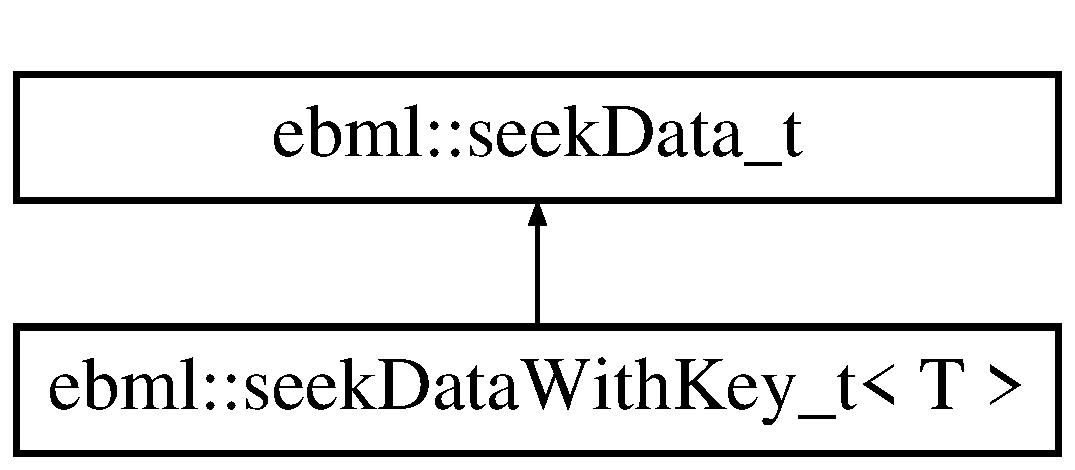
\includegraphics[height=2.000000cm]{classebml_1_1seekData__t}
\end{center}
\end{figure}
\subsection*{Public Member Functions}
\begin{DoxyCompactItemize}
\item 
\mbox{\hyperlink{classebml_1_1seekData__t_a080c97211758dcec4045e5e08427cdb1}{seek\+Data\+\_\+t}} (\mbox{\hyperlink{namespaceebml_a86c5f604ddf12a74aa9812e997a58691}{ebml\+I\+D\+\_\+t}}, off\+\_\+t, \mbox{\hyperlink{namespaceebml_a2ccdfb60b23efb51fe07f9d066e23604}{vint\+Width\+\_\+t}}, size\+\_\+t)
\item 
\mbox{\hyperlink{classebml_1_1seekData__t_ad64e95299ca85c695b33eb8230cbe48c}{seek\+Data\+\_\+t}} (\mbox{\hyperlink{namespaceebml_a86c5f604ddf12a74aa9812e997a58691}{ebml\+I\+D\+\_\+t}}, off\+\_\+t, \mbox{\hyperlink{namespaceebml_a2ccdfb60b23efb51fe07f9d066e23604}{vint\+Width\+\_\+t}}, size\+\_\+t, const \mbox{\hyperlink{namespaceebml_adad533b7705a16bb360fe56380c5e7be}{ebml\+Element\+\_\+sp}} \&)
\item 
\mbox{\hyperlink{classebml_1_1seekData__t_a4073e066b0e82681eb486e249a5a3ed2}{seek\+Data\+\_\+t}} (\mbox{\hyperlink{namespaceebml_a86c5f604ddf12a74aa9812e997a58691}{ebml\+I\+D\+\_\+t}}, off\+\_\+t, \mbox{\hyperlink{namespaceebml_a2ccdfb60b23efb51fe07f9d066e23604}{vint\+Width\+\_\+t}}, size\+\_\+t, const \mbox{\hyperlink{namespaceebml_adad533b7705a16bb360fe56380c5e7be}{ebml\+Element\+\_\+sp}} \&, const \mbox{\hyperlink{namespaceebml_adad533b7705a16bb360fe56380c5e7be}{ebml\+Element\+\_\+sp}} \&)
\item 
\mbox{\hyperlink{classebml_1_1seekData__t_a8df38b86c02a5cc3491970ae48605a29}{seek\+Data\+\_\+t}} (const \mbox{\hyperlink{classebml_1_1seekData__t}{seek\+Data\+\_\+t}} \&)
\item 
\mbox{\hyperlink{classebml_1_1seekData__t_a19592a08f48414ada236b0264be6c3b6}{seek\+Data\+\_\+t}} (\mbox{\hyperlink{classebml_1_1seekData__t}{seek\+Data\+\_\+t}} \&\&)
\item 
\mbox{\hyperlink{classebml_1_1seekData__t}{seek\+Data\+\_\+t}} \& \mbox{\hyperlink{classebml_1_1seekData__t_a9ecc0247b6026b2cfd055b302a620166}{operator=}} (const \mbox{\hyperlink{classebml_1_1seekData__t}{seek\+Data\+\_\+t}} \&)
\item 
\mbox{\hyperlink{classebml_1_1seekData__t}{seek\+Data\+\_\+t}} \& \mbox{\hyperlink{classebml_1_1seekData__t_a7e1b55089fe090b9c2412f140411e2c3}{operator=}} (\mbox{\hyperlink{classebml_1_1seekData__t}{seek\+Data\+\_\+t}} \&\&)
\item 
{\footnotesize template$<$typename T $>$ }\\\mbox{\hyperlink{classebml_1_1seekDataWithKey__t}{seek\+Data\+With\+Key\+\_\+t}}$<$ T $>$ \& \mbox{\hyperlink{classebml_1_1seekData__t_a1c5d23645387f0d93a078d2227893b50}{with\+Key\+Type}} ()
\item 
{\footnotesize template$<$typename T $>$ }\\const \mbox{\hyperlink{classebml_1_1seekDataWithKey__t}{seek\+Data\+With\+Key\+\_\+t}}$<$ T $>$ \& \mbox{\hyperlink{classebml_1_1seekData__t_aea1960bbf31310cf899420a7a36d5a49}{with\+Key\+Type}} () const
\item 
{\footnotesize template$<$typename T $>$ }\\T \& \mbox{\hyperlink{classebml_1_1seekData__t_a1dec5e33c576eecc5685796c28dca712}{key}} ()
\item 
{\footnotesize template$<$typename T $>$ }\\const T \& \mbox{\hyperlink{classebml_1_1seekData__t_a9a3356fbd22caa75a6df703e3e2f2ca6}{key}} () const
\item 
virtual void \mbox{\hyperlink{classebml_1_1seekData__t_a6ca62e902490d42a3dd03cfd23452016}{add}} (std\+::unordered\+\_\+map$<$ \mbox{\hyperlink{namespaceebml_a86c5f604ddf12a74aa9812e997a58691}{ebml\+I\+D\+\_\+t}}, std\+::unique\+\_\+ptr$<$ \mbox{\hyperlink{classebml_1_1seekMapBase}{seek\+Map\+Base}} $>$$>$ \&)
\item 
virtual void \mbox{\hyperlink{classebml_1_1seekData__t_a1f0da8c547bc52496bc4716ec732d138}{rm}} (std\+::unordered\+\_\+map$<$ \mbox{\hyperlink{namespaceebml_a86c5f604ddf12a74aa9812e997a58691}{ebml\+I\+D\+\_\+t}}, std\+::unique\+\_\+ptr$<$ \mbox{\hyperlink{classebml_1_1seekMapBase}{seek\+Map\+Base}} $>$$>$ \&)
\end{DoxyCompactItemize}
\subsection*{Public Attributes}
\begin{DoxyCompactItemize}
\item 
\mbox{\hyperlink{namespaceebml_a86c5f604ddf12a74aa9812e997a58691}{ebml\+I\+D\+\_\+t}} \mbox{\hyperlink{classebml_1_1seekData__t_aeebc9c60a3157c2e8963dff000016111}{ebml\+ID}}
\item 
off\+\_\+t \mbox{\hyperlink{classebml_1_1seekData__t_a0c34ad1abeed44ddb521abac8dfe107a}{offset\+In\+Parent}}
\item 
\mbox{\hyperlink{namespaceebml_a2ccdfb60b23efb51fe07f9d066e23604}{vint\+Width\+\_\+t}} \mbox{\hyperlink{classebml_1_1seekData__t_aaebccafee18298ba365b784acbc6df6b}{size\+Width}}
\item 
size\+\_\+t \mbox{\hyperlink{classebml_1_1seekData__t_a0a25256a0cd61d4077bb37e064198125}{data\+Size}}
\item 
\mbox{\hyperlink{namespaceebml_a495fb58b42b0050d887415351af02935}{ebml\+Element\+\_\+wp}} \mbox{\hyperlink{classebml_1_1seekData__t_af9e91ea27623cf9d36ef45f8202e4f46}{ref}}
\item 
\mbox{\hyperlink{namespaceebml_a495fb58b42b0050d887415351af02935}{ebml\+Element\+\_\+wp}} \mbox{\hyperlink{classebml_1_1seekData__t_aa2137b3e5ee53c2e90754fa44f81f2ef}{parent}}
\end{DoxyCompactItemize}


\subsection{Constructor \& Destructor Documentation}
\mbox{\Hypertarget{classebml_1_1seekData__t_a080c97211758dcec4045e5e08427cdb1}\label{classebml_1_1seekData__t_a080c97211758dcec4045e5e08427cdb1}} 
\index{ebml\+::seek\+Data\+\_\+t@{ebml\+::seek\+Data\+\_\+t}!seek\+Data\+\_\+t@{seek\+Data\+\_\+t}}
\index{seek\+Data\+\_\+t@{seek\+Data\+\_\+t}!ebml\+::seek\+Data\+\_\+t@{ebml\+::seek\+Data\+\_\+t}}
\subsubsection{\texorpdfstring{seek\+Data\+\_\+t()}{seekData\_t()}\hspace{0.1cm}{\footnotesize\ttfamily [1/5]}}
{\footnotesize\ttfamily ebml\+::seek\+Data\+\_\+t\+::seek\+Data\+\_\+t (\begin{DoxyParamCaption}\item[{\mbox{\hyperlink{namespaceebml_a86c5f604ddf12a74aa9812e997a58691}{ebml\+I\+D\+\_\+t}}}]{,  }\item[{off\+\_\+t}]{,  }\item[{\mbox{\hyperlink{namespaceebml_a2ccdfb60b23efb51fe07f9d066e23604}{vint\+Width\+\_\+t}}}]{,  }\item[{size\+\_\+t}]{ }\end{DoxyParamCaption})}

\mbox{\Hypertarget{classebml_1_1seekData__t_ad64e95299ca85c695b33eb8230cbe48c}\label{classebml_1_1seekData__t_ad64e95299ca85c695b33eb8230cbe48c}} 
\index{ebml\+::seek\+Data\+\_\+t@{ebml\+::seek\+Data\+\_\+t}!seek\+Data\+\_\+t@{seek\+Data\+\_\+t}}
\index{seek\+Data\+\_\+t@{seek\+Data\+\_\+t}!ebml\+::seek\+Data\+\_\+t@{ebml\+::seek\+Data\+\_\+t}}
\subsubsection{\texorpdfstring{seek\+Data\+\_\+t()}{seekData\_t()}\hspace{0.1cm}{\footnotesize\ttfamily [2/5]}}
{\footnotesize\ttfamily ebml\+::seek\+Data\+\_\+t\+::seek\+Data\+\_\+t (\begin{DoxyParamCaption}\item[{\mbox{\hyperlink{namespaceebml_a86c5f604ddf12a74aa9812e997a58691}{ebml\+I\+D\+\_\+t}}}]{,  }\item[{off\+\_\+t}]{,  }\item[{\mbox{\hyperlink{namespaceebml_a2ccdfb60b23efb51fe07f9d066e23604}{vint\+Width\+\_\+t}}}]{,  }\item[{size\+\_\+t}]{,  }\item[{const \mbox{\hyperlink{namespaceebml_adad533b7705a16bb360fe56380c5e7be}{ebml\+Element\+\_\+sp}} \&}]{ }\end{DoxyParamCaption})}

\mbox{\Hypertarget{classebml_1_1seekData__t_a4073e066b0e82681eb486e249a5a3ed2}\label{classebml_1_1seekData__t_a4073e066b0e82681eb486e249a5a3ed2}} 
\index{ebml\+::seek\+Data\+\_\+t@{ebml\+::seek\+Data\+\_\+t}!seek\+Data\+\_\+t@{seek\+Data\+\_\+t}}
\index{seek\+Data\+\_\+t@{seek\+Data\+\_\+t}!ebml\+::seek\+Data\+\_\+t@{ebml\+::seek\+Data\+\_\+t}}
\subsubsection{\texorpdfstring{seek\+Data\+\_\+t()}{seekData\_t()}\hspace{0.1cm}{\footnotesize\ttfamily [3/5]}}
{\footnotesize\ttfamily ebml\+::seek\+Data\+\_\+t\+::seek\+Data\+\_\+t (\begin{DoxyParamCaption}\item[{\mbox{\hyperlink{namespaceebml_a86c5f604ddf12a74aa9812e997a58691}{ebml\+I\+D\+\_\+t}}}]{,  }\item[{off\+\_\+t}]{,  }\item[{\mbox{\hyperlink{namespaceebml_a2ccdfb60b23efb51fe07f9d066e23604}{vint\+Width\+\_\+t}}}]{,  }\item[{size\+\_\+t}]{,  }\item[{const \mbox{\hyperlink{namespaceebml_adad533b7705a16bb360fe56380c5e7be}{ebml\+Element\+\_\+sp}} \&}]{,  }\item[{const \mbox{\hyperlink{namespaceebml_adad533b7705a16bb360fe56380c5e7be}{ebml\+Element\+\_\+sp}} \&}]{ }\end{DoxyParamCaption})}

\mbox{\Hypertarget{classebml_1_1seekData__t_a8df38b86c02a5cc3491970ae48605a29}\label{classebml_1_1seekData__t_a8df38b86c02a5cc3491970ae48605a29}} 
\index{ebml\+::seek\+Data\+\_\+t@{ebml\+::seek\+Data\+\_\+t}!seek\+Data\+\_\+t@{seek\+Data\+\_\+t}}
\index{seek\+Data\+\_\+t@{seek\+Data\+\_\+t}!ebml\+::seek\+Data\+\_\+t@{ebml\+::seek\+Data\+\_\+t}}
\subsubsection{\texorpdfstring{seek\+Data\+\_\+t()}{seekData\_t()}\hspace{0.1cm}{\footnotesize\ttfamily [4/5]}}
{\footnotesize\ttfamily ebml\+::seek\+Data\+\_\+t\+::seek\+Data\+\_\+t (\begin{DoxyParamCaption}\item[{const \mbox{\hyperlink{classebml_1_1seekData__t}{seek\+Data\+\_\+t}} \&}]{ }\end{DoxyParamCaption})}

\mbox{\Hypertarget{classebml_1_1seekData__t_a19592a08f48414ada236b0264be6c3b6}\label{classebml_1_1seekData__t_a19592a08f48414ada236b0264be6c3b6}} 
\index{ebml\+::seek\+Data\+\_\+t@{ebml\+::seek\+Data\+\_\+t}!seek\+Data\+\_\+t@{seek\+Data\+\_\+t}}
\index{seek\+Data\+\_\+t@{seek\+Data\+\_\+t}!ebml\+::seek\+Data\+\_\+t@{ebml\+::seek\+Data\+\_\+t}}
\subsubsection{\texorpdfstring{seek\+Data\+\_\+t()}{seekData\_t()}\hspace{0.1cm}{\footnotesize\ttfamily [5/5]}}
{\footnotesize\ttfamily ebml\+::seek\+Data\+\_\+t\+::seek\+Data\+\_\+t (\begin{DoxyParamCaption}\item[{\mbox{\hyperlink{classebml_1_1seekData__t}{seek\+Data\+\_\+t}} \&\&}]{ }\end{DoxyParamCaption})}



\subsection{Member Function Documentation}
\mbox{\Hypertarget{classebml_1_1seekData__t_a6ca62e902490d42a3dd03cfd23452016}\label{classebml_1_1seekData__t_a6ca62e902490d42a3dd03cfd23452016}} 
\index{ebml\+::seek\+Data\+\_\+t@{ebml\+::seek\+Data\+\_\+t}!add@{add}}
\index{add@{add}!ebml\+::seek\+Data\+\_\+t@{ebml\+::seek\+Data\+\_\+t}}
\subsubsection{\texorpdfstring{add()}{add()}}
{\footnotesize\ttfamily virtual void ebml\+::seek\+Data\+\_\+t\+::add (\begin{DoxyParamCaption}\item[{std\+::unordered\+\_\+map$<$ \mbox{\hyperlink{namespaceebml_a86c5f604ddf12a74aa9812e997a58691}{ebml\+I\+D\+\_\+t}}, std\+::unique\+\_\+ptr$<$ \mbox{\hyperlink{classebml_1_1seekMapBase}{seek\+Map\+Base}} $>$$>$ \&}]{ }\end{DoxyParamCaption})\hspace{0.3cm}{\ttfamily [virtual]}}



Reimplemented in \mbox{\hyperlink{classebml_1_1seekDataWithKey__t_a4997f1c29bd331a1e6d8c5293f7d4730}{ebml\+::seek\+Data\+With\+Key\+\_\+t$<$ T $>$}}.

\mbox{\Hypertarget{classebml_1_1seekData__t_a1dec5e33c576eecc5685796c28dca712}\label{classebml_1_1seekData__t_a1dec5e33c576eecc5685796c28dca712}} 
\index{ebml\+::seek\+Data\+\_\+t@{ebml\+::seek\+Data\+\_\+t}!key@{key}}
\index{key@{key}!ebml\+::seek\+Data\+\_\+t@{ebml\+::seek\+Data\+\_\+t}}
\subsubsection{\texorpdfstring{key()}{key()}\hspace{0.1cm}{\footnotesize\ttfamily [1/2]}}
{\footnotesize\ttfamily template$<$typename T $>$ \\
T\& ebml\+::seek\+Data\+\_\+t\+::key (\begin{DoxyParamCaption}{ }\end{DoxyParamCaption})}

\mbox{\Hypertarget{classebml_1_1seekData__t_a9a3356fbd22caa75a6df703e3e2f2ca6}\label{classebml_1_1seekData__t_a9a3356fbd22caa75a6df703e3e2f2ca6}} 
\index{ebml\+::seek\+Data\+\_\+t@{ebml\+::seek\+Data\+\_\+t}!key@{key}}
\index{key@{key}!ebml\+::seek\+Data\+\_\+t@{ebml\+::seek\+Data\+\_\+t}}
\subsubsection{\texorpdfstring{key()}{key()}\hspace{0.1cm}{\footnotesize\ttfamily [2/2]}}
{\footnotesize\ttfamily template$<$typename T $>$ \\
const T\& ebml\+::seek\+Data\+\_\+t\+::key (\begin{DoxyParamCaption}{ }\end{DoxyParamCaption}) const}

\mbox{\Hypertarget{classebml_1_1seekData__t_a9ecc0247b6026b2cfd055b302a620166}\label{classebml_1_1seekData__t_a9ecc0247b6026b2cfd055b302a620166}} 
\index{ebml\+::seek\+Data\+\_\+t@{ebml\+::seek\+Data\+\_\+t}!operator=@{operator=}}
\index{operator=@{operator=}!ebml\+::seek\+Data\+\_\+t@{ebml\+::seek\+Data\+\_\+t}}
\subsubsection{\texorpdfstring{operator=()}{operator=()}\hspace{0.1cm}{\footnotesize\ttfamily [1/2]}}
{\footnotesize\ttfamily \mbox{\hyperlink{classebml_1_1seekData__t}{seek\+Data\+\_\+t}}\& ebml\+::seek\+Data\+\_\+t\+::operator= (\begin{DoxyParamCaption}\item[{const \mbox{\hyperlink{classebml_1_1seekData__t}{seek\+Data\+\_\+t}} \&}]{ }\end{DoxyParamCaption})}

\mbox{\Hypertarget{classebml_1_1seekData__t_a7e1b55089fe090b9c2412f140411e2c3}\label{classebml_1_1seekData__t_a7e1b55089fe090b9c2412f140411e2c3}} 
\index{ebml\+::seek\+Data\+\_\+t@{ebml\+::seek\+Data\+\_\+t}!operator=@{operator=}}
\index{operator=@{operator=}!ebml\+::seek\+Data\+\_\+t@{ebml\+::seek\+Data\+\_\+t}}
\subsubsection{\texorpdfstring{operator=()}{operator=()}\hspace{0.1cm}{\footnotesize\ttfamily [2/2]}}
{\footnotesize\ttfamily \mbox{\hyperlink{classebml_1_1seekData__t}{seek\+Data\+\_\+t}}\& ebml\+::seek\+Data\+\_\+t\+::operator= (\begin{DoxyParamCaption}\item[{\mbox{\hyperlink{classebml_1_1seekData__t}{seek\+Data\+\_\+t}} \&\&}]{ }\end{DoxyParamCaption})}

\mbox{\Hypertarget{classebml_1_1seekData__t_a1f0da8c547bc52496bc4716ec732d138}\label{classebml_1_1seekData__t_a1f0da8c547bc52496bc4716ec732d138}} 
\index{ebml\+::seek\+Data\+\_\+t@{ebml\+::seek\+Data\+\_\+t}!rm@{rm}}
\index{rm@{rm}!ebml\+::seek\+Data\+\_\+t@{ebml\+::seek\+Data\+\_\+t}}
\subsubsection{\texorpdfstring{rm()}{rm()}}
{\footnotesize\ttfamily virtual void ebml\+::seek\+Data\+\_\+t\+::rm (\begin{DoxyParamCaption}\item[{std\+::unordered\+\_\+map$<$ \mbox{\hyperlink{namespaceebml_a86c5f604ddf12a74aa9812e997a58691}{ebml\+I\+D\+\_\+t}}, std\+::unique\+\_\+ptr$<$ \mbox{\hyperlink{classebml_1_1seekMapBase}{seek\+Map\+Base}} $>$$>$ \&}]{ }\end{DoxyParamCaption})\hspace{0.3cm}{\ttfamily [virtual]}}



Reimplemented in \mbox{\hyperlink{classebml_1_1seekDataWithKey__t_afc028f689e5c536e26ca8619d6dbb0a2}{ebml\+::seek\+Data\+With\+Key\+\_\+t$<$ T $>$}}.

\mbox{\Hypertarget{classebml_1_1seekData__t_a1c5d23645387f0d93a078d2227893b50}\label{classebml_1_1seekData__t_a1c5d23645387f0d93a078d2227893b50}} 
\index{ebml\+::seek\+Data\+\_\+t@{ebml\+::seek\+Data\+\_\+t}!with\+Key\+Type@{with\+Key\+Type}}
\index{with\+Key\+Type@{with\+Key\+Type}!ebml\+::seek\+Data\+\_\+t@{ebml\+::seek\+Data\+\_\+t}}
\subsubsection{\texorpdfstring{with\+Key\+Type()}{withKeyType()}\hspace{0.1cm}{\footnotesize\ttfamily [1/2]}}
{\footnotesize\ttfamily template$<$typename T $>$ \\
\mbox{\hyperlink{classebml_1_1seekDataWithKey__t}{seek\+Data\+With\+Key\+\_\+t}}$<$T$>$\& ebml\+::seek\+Data\+\_\+t\+::with\+Key\+Type (\begin{DoxyParamCaption}{ }\end{DoxyParamCaption})}

\mbox{\Hypertarget{classebml_1_1seekData__t_aea1960bbf31310cf899420a7a36d5a49}\label{classebml_1_1seekData__t_aea1960bbf31310cf899420a7a36d5a49}} 
\index{ebml\+::seek\+Data\+\_\+t@{ebml\+::seek\+Data\+\_\+t}!with\+Key\+Type@{with\+Key\+Type}}
\index{with\+Key\+Type@{with\+Key\+Type}!ebml\+::seek\+Data\+\_\+t@{ebml\+::seek\+Data\+\_\+t}}
\subsubsection{\texorpdfstring{with\+Key\+Type()}{withKeyType()}\hspace{0.1cm}{\footnotesize\ttfamily [2/2]}}
{\footnotesize\ttfamily template$<$typename T $>$ \\
const \mbox{\hyperlink{classebml_1_1seekDataWithKey__t}{seek\+Data\+With\+Key\+\_\+t}}$<$T$>$\& ebml\+::seek\+Data\+\_\+t\+::with\+Key\+Type (\begin{DoxyParamCaption}{ }\end{DoxyParamCaption}) const}



\subsection{Member Data Documentation}
\mbox{\Hypertarget{classebml_1_1seekData__t_a0a25256a0cd61d4077bb37e064198125}\label{classebml_1_1seekData__t_a0a25256a0cd61d4077bb37e064198125}} 
\index{ebml\+::seek\+Data\+\_\+t@{ebml\+::seek\+Data\+\_\+t}!data\+Size@{data\+Size}}
\index{data\+Size@{data\+Size}!ebml\+::seek\+Data\+\_\+t@{ebml\+::seek\+Data\+\_\+t}}
\subsubsection{\texorpdfstring{data\+Size}{dataSize}}
{\footnotesize\ttfamily size\+\_\+t ebml\+::seek\+Data\+\_\+t\+::data\+Size}

\mbox{\Hypertarget{classebml_1_1seekData__t_aeebc9c60a3157c2e8963dff000016111}\label{classebml_1_1seekData__t_aeebc9c60a3157c2e8963dff000016111}} 
\index{ebml\+::seek\+Data\+\_\+t@{ebml\+::seek\+Data\+\_\+t}!ebml\+ID@{ebml\+ID}}
\index{ebml\+ID@{ebml\+ID}!ebml\+::seek\+Data\+\_\+t@{ebml\+::seek\+Data\+\_\+t}}
\subsubsection{\texorpdfstring{ebml\+ID}{ebmlID}}
{\footnotesize\ttfamily \mbox{\hyperlink{namespaceebml_a86c5f604ddf12a74aa9812e997a58691}{ebml\+I\+D\+\_\+t}} ebml\+::seek\+Data\+\_\+t\+::ebml\+ID}

\mbox{\Hypertarget{classebml_1_1seekData__t_a0c34ad1abeed44ddb521abac8dfe107a}\label{classebml_1_1seekData__t_a0c34ad1abeed44ddb521abac8dfe107a}} 
\index{ebml\+::seek\+Data\+\_\+t@{ebml\+::seek\+Data\+\_\+t}!offset\+In\+Parent@{offset\+In\+Parent}}
\index{offset\+In\+Parent@{offset\+In\+Parent}!ebml\+::seek\+Data\+\_\+t@{ebml\+::seek\+Data\+\_\+t}}
\subsubsection{\texorpdfstring{offset\+In\+Parent}{offsetInParent}}
{\footnotesize\ttfamily off\+\_\+t ebml\+::seek\+Data\+\_\+t\+::offset\+In\+Parent}

\mbox{\Hypertarget{classebml_1_1seekData__t_aa2137b3e5ee53c2e90754fa44f81f2ef}\label{classebml_1_1seekData__t_aa2137b3e5ee53c2e90754fa44f81f2ef}} 
\index{ebml\+::seek\+Data\+\_\+t@{ebml\+::seek\+Data\+\_\+t}!parent@{parent}}
\index{parent@{parent}!ebml\+::seek\+Data\+\_\+t@{ebml\+::seek\+Data\+\_\+t}}
\subsubsection{\texorpdfstring{parent}{parent}}
{\footnotesize\ttfamily \mbox{\hyperlink{namespaceebml_a495fb58b42b0050d887415351af02935}{ebml\+Element\+\_\+wp}} ebml\+::seek\+Data\+\_\+t\+::parent}

\mbox{\Hypertarget{classebml_1_1seekData__t_af9e91ea27623cf9d36ef45f8202e4f46}\label{classebml_1_1seekData__t_af9e91ea27623cf9d36ef45f8202e4f46}} 
\index{ebml\+::seek\+Data\+\_\+t@{ebml\+::seek\+Data\+\_\+t}!ref@{ref}}
\index{ref@{ref}!ebml\+::seek\+Data\+\_\+t@{ebml\+::seek\+Data\+\_\+t}}
\subsubsection{\texorpdfstring{ref}{ref}}
{\footnotesize\ttfamily \mbox{\hyperlink{namespaceebml_a495fb58b42b0050d887415351af02935}{ebml\+Element\+\_\+wp}} ebml\+::seek\+Data\+\_\+t\+::ref}

\mbox{\Hypertarget{classebml_1_1seekData__t_aaebccafee18298ba365b784acbc6df6b}\label{classebml_1_1seekData__t_aaebccafee18298ba365b784acbc6df6b}} 
\index{ebml\+::seek\+Data\+\_\+t@{ebml\+::seek\+Data\+\_\+t}!size\+Width@{size\+Width}}
\index{size\+Width@{size\+Width}!ebml\+::seek\+Data\+\_\+t@{ebml\+::seek\+Data\+\_\+t}}
\subsubsection{\texorpdfstring{size\+Width}{sizeWidth}}
{\footnotesize\ttfamily \mbox{\hyperlink{namespaceebml_a2ccdfb60b23efb51fe07f9d066e23604}{vint\+Width\+\_\+t}} ebml\+::seek\+Data\+\_\+t\+::size\+Width}



The documentation for this class was generated from the following file\+:\begin{DoxyCompactItemize}
\item 
include/libebml\+\_\+ng/\mbox{\hyperlink{seekdata_8h}{seekdata.\+h}}\end{DoxyCompactItemize}

\hypertarget{classebml_1_1seekDataWithKey__t}{}\section{ebml\+:\+:seek\+Data\+With\+Key\+\_\+t$<$ T $>$ Class Template Reference}
\label{classebml_1_1seekDataWithKey__t}\index{ebml\+::seek\+Data\+With\+Key\+\_\+t$<$ T $>$@{ebml\+::seek\+Data\+With\+Key\+\_\+t$<$ T $>$}}


{\ttfamily \#include $<$seekdata.\+h$>$}

Inheritance diagram for ebml\+:\+:seek\+Data\+With\+Key\+\_\+t$<$ T $>$\+:\begin{figure}[H]
\begin{center}
\leavevmode
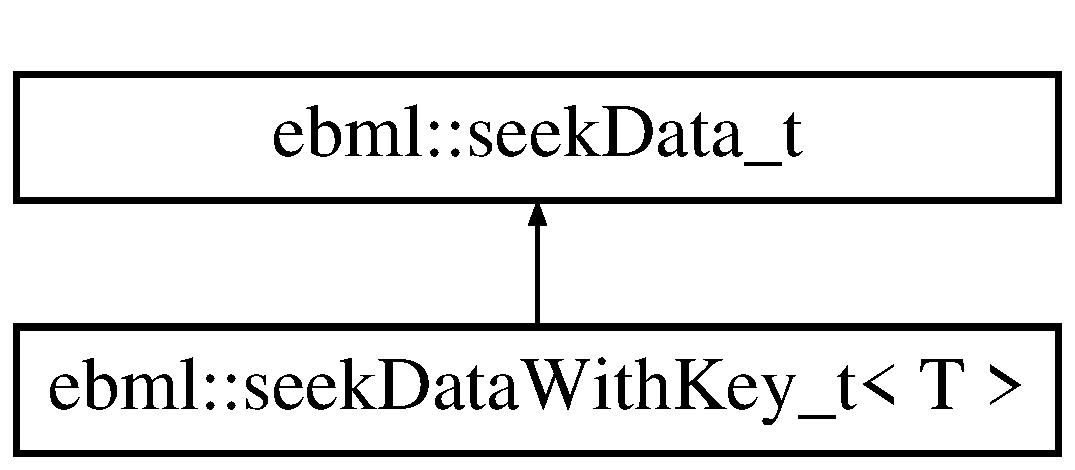
\includegraphics[height=2.000000cm]{classebml_1_1seekDataWithKey__t}
\end{center}
\end{figure}
\subsection*{Public Member Functions}
\begin{DoxyCompactItemize}
\item 
void \mbox{\hyperlink{classebml_1_1seekDataWithKey__t_a4997f1c29bd331a1e6d8c5293f7d4730}{add}} (std\+::unordered\+\_\+map$<$ \mbox{\hyperlink{namespaceebml_a86c5f604ddf12a74aa9812e997a58691}{ebml\+I\+D\+\_\+t}}, std\+::unique\+\_\+ptr$<$ \mbox{\hyperlink{classebml_1_1seekMapBase}{seek\+Map\+Base}} $>$$>$ \&)
\item 
void \mbox{\hyperlink{classebml_1_1seekDataWithKey__t_afc028f689e5c536e26ca8619d6dbb0a2}{rm}} (std\+::unordered\+\_\+map$<$ \mbox{\hyperlink{namespaceebml_a86c5f604ddf12a74aa9812e997a58691}{ebml\+I\+D\+\_\+t}}, std\+::unique\+\_\+ptr$<$ \mbox{\hyperlink{classebml_1_1seekMapBase}{seek\+Map\+Base}} $>$$>$ \&)
\item 
\mbox{\hyperlink{classebml_1_1seekDataWithKey__t_a01ce559343d7fd9ab658f3b71d6ed448}{seek\+Data\+With\+Key\+\_\+t}} (\mbox{\hyperlink{namespaceebml_a86c5f604ddf12a74aa9812e997a58691}{ebml\+I\+D\+\_\+t}}, off\+\_\+t, \mbox{\hyperlink{namespaceebml_a2ccdfb60b23efb51fe07f9d066e23604}{vint\+Width\+\_\+t}}, size\+\_\+t, const T \&)
\item 
\mbox{\hyperlink{classebml_1_1seekDataWithKey__t_abe19a3272fbe18811c86e08cb0eba108}{seek\+Data\+With\+Key\+\_\+t}} (\mbox{\hyperlink{namespaceebml_a86c5f604ddf12a74aa9812e997a58691}{ebml\+I\+D\+\_\+t}}, off\+\_\+t, \mbox{\hyperlink{namespaceebml_a2ccdfb60b23efb51fe07f9d066e23604}{vint\+Width\+\_\+t}}, size\+\_\+t, T \&\&)
\item 
\mbox{\hyperlink{classebml_1_1seekDataWithKey__t_a2e92d63c712630d15c19742fb215f512}{seek\+Data\+With\+Key\+\_\+t}} (\mbox{\hyperlink{namespaceebml_a86c5f604ddf12a74aa9812e997a58691}{ebml\+I\+D\+\_\+t}}, off\+\_\+t, \mbox{\hyperlink{namespaceebml_a2ccdfb60b23efb51fe07f9d066e23604}{vint\+Width\+\_\+t}}, size\+\_\+t, const T \&, const \mbox{\hyperlink{namespaceebml_adad533b7705a16bb360fe56380c5e7be}{ebml\+Element\+\_\+sp}} \&)
\item 
\mbox{\hyperlink{classebml_1_1seekDataWithKey__t_a8d13d1e10002ba82e2f8c9be9ed60464}{seek\+Data\+With\+Key\+\_\+t}} (\mbox{\hyperlink{namespaceebml_a86c5f604ddf12a74aa9812e997a58691}{ebml\+I\+D\+\_\+t}}, off\+\_\+t, \mbox{\hyperlink{namespaceebml_a2ccdfb60b23efb51fe07f9d066e23604}{vint\+Width\+\_\+t}}, size\+\_\+t, const T \&, const \mbox{\hyperlink{namespaceebml_adad533b7705a16bb360fe56380c5e7be}{ebml\+Element\+\_\+sp}} \&, const \mbox{\hyperlink{namespaceebml_adad533b7705a16bb360fe56380c5e7be}{ebml\+Element\+\_\+sp}} \&)
\item 
\mbox{\hyperlink{classebml_1_1seekDataWithKey__t_a48a97c3a5b493a689a837e6f1d859469}{seek\+Data\+With\+Key\+\_\+t}} (\mbox{\hyperlink{namespaceebml_a86c5f604ddf12a74aa9812e997a58691}{ebml\+I\+D\+\_\+t}}, off\+\_\+t, \mbox{\hyperlink{namespaceebml_a2ccdfb60b23efb51fe07f9d066e23604}{vint\+Width\+\_\+t}}, size\+\_\+t, T \&\&, const \mbox{\hyperlink{namespaceebml_adad533b7705a16bb360fe56380c5e7be}{ebml\+Element\+\_\+sp}} \&)
\item 
\mbox{\hyperlink{classebml_1_1seekDataWithKey__t_a96571489016319c689963ab35f694e91}{seek\+Data\+With\+Key\+\_\+t}} (\mbox{\hyperlink{namespaceebml_a86c5f604ddf12a74aa9812e997a58691}{ebml\+I\+D\+\_\+t}}, off\+\_\+t, \mbox{\hyperlink{namespaceebml_a2ccdfb60b23efb51fe07f9d066e23604}{vint\+Width\+\_\+t}}, size\+\_\+t, T \&\&, const \mbox{\hyperlink{namespaceebml_adad533b7705a16bb360fe56380c5e7be}{ebml\+Element\+\_\+sp}} \&, const \mbox{\hyperlink{namespaceebml_adad533b7705a16bb360fe56380c5e7be}{ebml\+Element\+\_\+sp}} \&)
\end{DoxyCompactItemize}
\subsection*{Public Attributes}
\begin{DoxyCompactItemize}
\item 
T \mbox{\hyperlink{classebml_1_1seekDataWithKey__t_a5cc5af451ed608f03c4e68ef29651d9c}{key}}
\end{DoxyCompactItemize}


\subsection{Constructor \& Destructor Documentation}
\mbox{\Hypertarget{classebml_1_1seekDataWithKey__t_a01ce559343d7fd9ab658f3b71d6ed448}\label{classebml_1_1seekDataWithKey__t_a01ce559343d7fd9ab658f3b71d6ed448}} 
\index{ebml\+::seek\+Data\+With\+Key\+\_\+t@{ebml\+::seek\+Data\+With\+Key\+\_\+t}!seek\+Data\+With\+Key\+\_\+t@{seek\+Data\+With\+Key\+\_\+t}}
\index{seek\+Data\+With\+Key\+\_\+t@{seek\+Data\+With\+Key\+\_\+t}!ebml\+::seek\+Data\+With\+Key\+\_\+t@{ebml\+::seek\+Data\+With\+Key\+\_\+t}}
\subsubsection{\texorpdfstring{seek\+Data\+With\+Key\+\_\+t()}{seekDataWithKey\_t()}\hspace{0.1cm}{\footnotesize\ttfamily [1/6]}}
{\footnotesize\ttfamily template$<$typename T$>$ \\
\mbox{\hyperlink{classebml_1_1seekDataWithKey__t}{ebml\+::seek\+Data\+With\+Key\+\_\+t}}$<$ T $>$\+::\mbox{\hyperlink{classebml_1_1seekDataWithKey__t}{seek\+Data\+With\+Key\+\_\+t}} (\begin{DoxyParamCaption}\item[{\mbox{\hyperlink{namespaceebml_a86c5f604ddf12a74aa9812e997a58691}{ebml\+I\+D\+\_\+t}}}]{,  }\item[{off\+\_\+t}]{,  }\item[{\mbox{\hyperlink{namespaceebml_a2ccdfb60b23efb51fe07f9d066e23604}{vint\+Width\+\_\+t}}}]{,  }\item[{size\+\_\+t}]{,  }\item[{const T \&}]{ }\end{DoxyParamCaption})}

\mbox{\Hypertarget{classebml_1_1seekDataWithKey__t_abe19a3272fbe18811c86e08cb0eba108}\label{classebml_1_1seekDataWithKey__t_abe19a3272fbe18811c86e08cb0eba108}} 
\index{ebml\+::seek\+Data\+With\+Key\+\_\+t@{ebml\+::seek\+Data\+With\+Key\+\_\+t}!seek\+Data\+With\+Key\+\_\+t@{seek\+Data\+With\+Key\+\_\+t}}
\index{seek\+Data\+With\+Key\+\_\+t@{seek\+Data\+With\+Key\+\_\+t}!ebml\+::seek\+Data\+With\+Key\+\_\+t@{ebml\+::seek\+Data\+With\+Key\+\_\+t}}
\subsubsection{\texorpdfstring{seek\+Data\+With\+Key\+\_\+t()}{seekDataWithKey\_t()}\hspace{0.1cm}{\footnotesize\ttfamily [2/6]}}
{\footnotesize\ttfamily template$<$typename T$>$ \\
\mbox{\hyperlink{classebml_1_1seekDataWithKey__t}{ebml\+::seek\+Data\+With\+Key\+\_\+t}}$<$ T $>$\+::\mbox{\hyperlink{classebml_1_1seekDataWithKey__t}{seek\+Data\+With\+Key\+\_\+t}} (\begin{DoxyParamCaption}\item[{\mbox{\hyperlink{namespaceebml_a86c5f604ddf12a74aa9812e997a58691}{ebml\+I\+D\+\_\+t}}}]{,  }\item[{off\+\_\+t}]{,  }\item[{\mbox{\hyperlink{namespaceebml_a2ccdfb60b23efb51fe07f9d066e23604}{vint\+Width\+\_\+t}}}]{,  }\item[{size\+\_\+t}]{,  }\item[{T \&\&}]{ }\end{DoxyParamCaption})}

\mbox{\Hypertarget{classebml_1_1seekDataWithKey__t_a2e92d63c712630d15c19742fb215f512}\label{classebml_1_1seekDataWithKey__t_a2e92d63c712630d15c19742fb215f512}} 
\index{ebml\+::seek\+Data\+With\+Key\+\_\+t@{ebml\+::seek\+Data\+With\+Key\+\_\+t}!seek\+Data\+With\+Key\+\_\+t@{seek\+Data\+With\+Key\+\_\+t}}
\index{seek\+Data\+With\+Key\+\_\+t@{seek\+Data\+With\+Key\+\_\+t}!ebml\+::seek\+Data\+With\+Key\+\_\+t@{ebml\+::seek\+Data\+With\+Key\+\_\+t}}
\subsubsection{\texorpdfstring{seek\+Data\+With\+Key\+\_\+t()}{seekDataWithKey\_t()}\hspace{0.1cm}{\footnotesize\ttfamily [3/6]}}
{\footnotesize\ttfamily template$<$typename T$>$ \\
\mbox{\hyperlink{classebml_1_1seekDataWithKey__t}{ebml\+::seek\+Data\+With\+Key\+\_\+t}}$<$ T $>$\+::\mbox{\hyperlink{classebml_1_1seekDataWithKey__t}{seek\+Data\+With\+Key\+\_\+t}} (\begin{DoxyParamCaption}\item[{\mbox{\hyperlink{namespaceebml_a86c5f604ddf12a74aa9812e997a58691}{ebml\+I\+D\+\_\+t}}}]{,  }\item[{off\+\_\+t}]{,  }\item[{\mbox{\hyperlink{namespaceebml_a2ccdfb60b23efb51fe07f9d066e23604}{vint\+Width\+\_\+t}}}]{,  }\item[{size\+\_\+t}]{,  }\item[{const T \&}]{,  }\item[{const \mbox{\hyperlink{namespaceebml_adad533b7705a16bb360fe56380c5e7be}{ebml\+Element\+\_\+sp}} \&}]{ }\end{DoxyParamCaption})}

\mbox{\Hypertarget{classebml_1_1seekDataWithKey__t_a8d13d1e10002ba82e2f8c9be9ed60464}\label{classebml_1_1seekDataWithKey__t_a8d13d1e10002ba82e2f8c9be9ed60464}} 
\index{ebml\+::seek\+Data\+With\+Key\+\_\+t@{ebml\+::seek\+Data\+With\+Key\+\_\+t}!seek\+Data\+With\+Key\+\_\+t@{seek\+Data\+With\+Key\+\_\+t}}
\index{seek\+Data\+With\+Key\+\_\+t@{seek\+Data\+With\+Key\+\_\+t}!ebml\+::seek\+Data\+With\+Key\+\_\+t@{ebml\+::seek\+Data\+With\+Key\+\_\+t}}
\subsubsection{\texorpdfstring{seek\+Data\+With\+Key\+\_\+t()}{seekDataWithKey\_t()}\hspace{0.1cm}{\footnotesize\ttfamily [4/6]}}
{\footnotesize\ttfamily template$<$typename T$>$ \\
\mbox{\hyperlink{classebml_1_1seekDataWithKey__t}{ebml\+::seek\+Data\+With\+Key\+\_\+t}}$<$ T $>$\+::\mbox{\hyperlink{classebml_1_1seekDataWithKey__t}{seek\+Data\+With\+Key\+\_\+t}} (\begin{DoxyParamCaption}\item[{\mbox{\hyperlink{namespaceebml_a86c5f604ddf12a74aa9812e997a58691}{ebml\+I\+D\+\_\+t}}}]{,  }\item[{off\+\_\+t}]{,  }\item[{\mbox{\hyperlink{namespaceebml_a2ccdfb60b23efb51fe07f9d066e23604}{vint\+Width\+\_\+t}}}]{,  }\item[{size\+\_\+t}]{,  }\item[{const T \&}]{,  }\item[{const \mbox{\hyperlink{namespaceebml_adad533b7705a16bb360fe56380c5e7be}{ebml\+Element\+\_\+sp}} \&}]{,  }\item[{const \mbox{\hyperlink{namespaceebml_adad533b7705a16bb360fe56380c5e7be}{ebml\+Element\+\_\+sp}} \&}]{ }\end{DoxyParamCaption})}

\mbox{\Hypertarget{classebml_1_1seekDataWithKey__t_a48a97c3a5b493a689a837e6f1d859469}\label{classebml_1_1seekDataWithKey__t_a48a97c3a5b493a689a837e6f1d859469}} 
\index{ebml\+::seek\+Data\+With\+Key\+\_\+t@{ebml\+::seek\+Data\+With\+Key\+\_\+t}!seek\+Data\+With\+Key\+\_\+t@{seek\+Data\+With\+Key\+\_\+t}}
\index{seek\+Data\+With\+Key\+\_\+t@{seek\+Data\+With\+Key\+\_\+t}!ebml\+::seek\+Data\+With\+Key\+\_\+t@{ebml\+::seek\+Data\+With\+Key\+\_\+t}}
\subsubsection{\texorpdfstring{seek\+Data\+With\+Key\+\_\+t()}{seekDataWithKey\_t()}\hspace{0.1cm}{\footnotesize\ttfamily [5/6]}}
{\footnotesize\ttfamily template$<$typename T$>$ \\
\mbox{\hyperlink{classebml_1_1seekDataWithKey__t}{ebml\+::seek\+Data\+With\+Key\+\_\+t}}$<$ T $>$\+::\mbox{\hyperlink{classebml_1_1seekDataWithKey__t}{seek\+Data\+With\+Key\+\_\+t}} (\begin{DoxyParamCaption}\item[{\mbox{\hyperlink{namespaceebml_a86c5f604ddf12a74aa9812e997a58691}{ebml\+I\+D\+\_\+t}}}]{,  }\item[{off\+\_\+t}]{,  }\item[{\mbox{\hyperlink{namespaceebml_a2ccdfb60b23efb51fe07f9d066e23604}{vint\+Width\+\_\+t}}}]{,  }\item[{size\+\_\+t}]{,  }\item[{T \&\&}]{,  }\item[{const \mbox{\hyperlink{namespaceebml_adad533b7705a16bb360fe56380c5e7be}{ebml\+Element\+\_\+sp}} \&}]{ }\end{DoxyParamCaption})}

\mbox{\Hypertarget{classebml_1_1seekDataWithKey__t_a96571489016319c689963ab35f694e91}\label{classebml_1_1seekDataWithKey__t_a96571489016319c689963ab35f694e91}} 
\index{ebml\+::seek\+Data\+With\+Key\+\_\+t@{ebml\+::seek\+Data\+With\+Key\+\_\+t}!seek\+Data\+With\+Key\+\_\+t@{seek\+Data\+With\+Key\+\_\+t}}
\index{seek\+Data\+With\+Key\+\_\+t@{seek\+Data\+With\+Key\+\_\+t}!ebml\+::seek\+Data\+With\+Key\+\_\+t@{ebml\+::seek\+Data\+With\+Key\+\_\+t}}
\subsubsection{\texorpdfstring{seek\+Data\+With\+Key\+\_\+t()}{seekDataWithKey\_t()}\hspace{0.1cm}{\footnotesize\ttfamily [6/6]}}
{\footnotesize\ttfamily template$<$typename T$>$ \\
\mbox{\hyperlink{classebml_1_1seekDataWithKey__t}{ebml\+::seek\+Data\+With\+Key\+\_\+t}}$<$ T $>$\+::\mbox{\hyperlink{classebml_1_1seekDataWithKey__t}{seek\+Data\+With\+Key\+\_\+t}} (\begin{DoxyParamCaption}\item[{\mbox{\hyperlink{namespaceebml_a86c5f604ddf12a74aa9812e997a58691}{ebml\+I\+D\+\_\+t}}}]{,  }\item[{off\+\_\+t}]{,  }\item[{\mbox{\hyperlink{namespaceebml_a2ccdfb60b23efb51fe07f9d066e23604}{vint\+Width\+\_\+t}}}]{,  }\item[{size\+\_\+t}]{,  }\item[{T \&\&}]{,  }\item[{const \mbox{\hyperlink{namespaceebml_adad533b7705a16bb360fe56380c5e7be}{ebml\+Element\+\_\+sp}} \&}]{,  }\item[{const \mbox{\hyperlink{namespaceebml_adad533b7705a16bb360fe56380c5e7be}{ebml\+Element\+\_\+sp}} \&}]{ }\end{DoxyParamCaption})}



\subsection{Member Function Documentation}
\mbox{\Hypertarget{classebml_1_1seekDataWithKey__t_a4997f1c29bd331a1e6d8c5293f7d4730}\label{classebml_1_1seekDataWithKey__t_a4997f1c29bd331a1e6d8c5293f7d4730}} 
\index{ebml\+::seek\+Data\+With\+Key\+\_\+t@{ebml\+::seek\+Data\+With\+Key\+\_\+t}!add@{add}}
\index{add@{add}!ebml\+::seek\+Data\+With\+Key\+\_\+t@{ebml\+::seek\+Data\+With\+Key\+\_\+t}}
\subsubsection{\texorpdfstring{add()}{add()}}
{\footnotesize\ttfamily template$<$typename T$>$ \\
void \mbox{\hyperlink{classebml_1_1seekDataWithKey__t}{ebml\+::seek\+Data\+With\+Key\+\_\+t}}$<$ T $>$\+::add (\begin{DoxyParamCaption}\item[{std\+::unordered\+\_\+map$<$ \mbox{\hyperlink{namespaceebml_a86c5f604ddf12a74aa9812e997a58691}{ebml\+I\+D\+\_\+t}}, std\+::unique\+\_\+ptr$<$ \mbox{\hyperlink{classebml_1_1seekMapBase}{seek\+Map\+Base}} $>$$>$ \&}]{ }\end{DoxyParamCaption})\hspace{0.3cm}{\ttfamily [virtual]}}



Reimplemented from \mbox{\hyperlink{classebml_1_1seekData__t_a6ca62e902490d42a3dd03cfd23452016}{ebml\+::seek\+Data\+\_\+t}}.

\mbox{\Hypertarget{classebml_1_1seekDataWithKey__t_afc028f689e5c536e26ca8619d6dbb0a2}\label{classebml_1_1seekDataWithKey__t_afc028f689e5c536e26ca8619d6dbb0a2}} 
\index{ebml\+::seek\+Data\+With\+Key\+\_\+t@{ebml\+::seek\+Data\+With\+Key\+\_\+t}!rm@{rm}}
\index{rm@{rm}!ebml\+::seek\+Data\+With\+Key\+\_\+t@{ebml\+::seek\+Data\+With\+Key\+\_\+t}}
\subsubsection{\texorpdfstring{rm()}{rm()}}
{\footnotesize\ttfamily template$<$typename T$>$ \\
void \mbox{\hyperlink{classebml_1_1seekDataWithKey__t}{ebml\+::seek\+Data\+With\+Key\+\_\+t}}$<$ T $>$\+::rm (\begin{DoxyParamCaption}\item[{std\+::unordered\+\_\+map$<$ \mbox{\hyperlink{namespaceebml_a86c5f604ddf12a74aa9812e997a58691}{ebml\+I\+D\+\_\+t}}, std\+::unique\+\_\+ptr$<$ \mbox{\hyperlink{classebml_1_1seekMapBase}{seek\+Map\+Base}} $>$$>$ \&}]{ }\end{DoxyParamCaption})\hspace{0.3cm}{\ttfamily [virtual]}}



Reimplemented from \mbox{\hyperlink{classebml_1_1seekData__t_a1f0da8c547bc52496bc4716ec732d138}{ebml\+::seek\+Data\+\_\+t}}.



\subsection{Member Data Documentation}
\mbox{\Hypertarget{classebml_1_1seekDataWithKey__t_a5cc5af451ed608f03c4e68ef29651d9c}\label{classebml_1_1seekDataWithKey__t_a5cc5af451ed608f03c4e68ef29651d9c}} 
\index{ebml\+::seek\+Data\+With\+Key\+\_\+t@{ebml\+::seek\+Data\+With\+Key\+\_\+t}!key@{key}}
\index{key@{key}!ebml\+::seek\+Data\+With\+Key\+\_\+t@{ebml\+::seek\+Data\+With\+Key\+\_\+t}}
\subsubsection{\texorpdfstring{key}{key}}
{\footnotesize\ttfamily template$<$typename T$>$ \\
T \mbox{\hyperlink{classebml_1_1seekDataWithKey__t}{ebml\+::seek\+Data\+With\+Key\+\_\+t}}$<$ T $>$\+::key}



The documentation for this class was generated from the following file\+:\begin{DoxyCompactItemize}
\item 
include/libebml\+\_\+ng/\mbox{\hyperlink{seekdata_8h}{seekdata.\+h}}\end{DoxyCompactItemize}

\hypertarget{classebml_1_1seekMap}{}\section{ebml\+:\+:seek\+Map$<$ T $>$ Class Template Reference}
\label{classebml_1_1seekMap}\index{ebml\+::seek\+Map$<$ T $>$@{ebml\+::seek\+Map$<$ T $>$}}


{\ttfamily \#include $<$seekdata.\+h$>$}

Inheritance diagram for ebml\+:\+:seek\+Map$<$ T $>$\+:\begin{figure}[H]
\begin{center}
\leavevmode
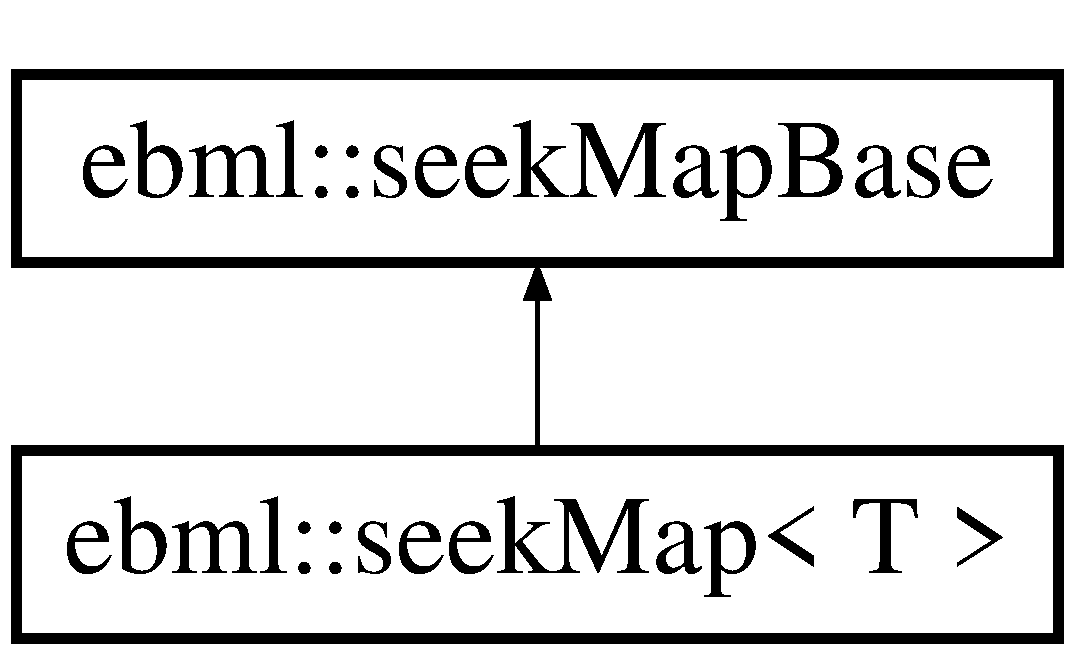
\includegraphics[height=2.000000cm]{classebml_1_1seekMap}
\end{center}
\end{figure}
\subsection*{Public Member Functions}
\begin{DoxyCompactItemize}
\item 
\mbox{\hyperlink{classebml_1_1seekDataWithKey__t}{seek\+Data\+With\+Key\+\_\+t}}$<$ T $>$ $\ast$\& \mbox{\hyperlink{classebml_1_1seekMap_ada2dfac4d3ed8f6046703a3385afc3d5}{operator\mbox{[}$\,$\mbox{]}}} (const T \&t)
\item 
\mbox{\hyperlink{classebml_1_1seekDataWithKey__t}{seek\+Data\+With\+Key\+\_\+t}}$<$ T $>$ $\ast$\& \mbox{\hyperlink{classebml_1_1seekMap_af99606cf546d3e99e6445a0baf5a6cad}{at}} (const T \&t)
\item 
\mbox{\hyperlink{classebml_1_1seekDataWithKey__t}{seek\+Data\+With\+Key\+\_\+t}}$<$ T $>$ $\ast$const  \& \mbox{\hyperlink{classebml_1_1seekMap_a4ec29d60a1d8b8edd825499dc87498b1}{at}} (const T \&) const
\item 
size\+\_\+t \mbox{\hyperlink{classebml_1_1seekMap_aa23bfd6f97470e3961143475031e84bd}{count}} (const T \&t) const
\item 
size\+\_\+t \mbox{\hyperlink{classebml_1_1seekMap_aba83cd8b8a60bd460bfe78acf1d04616}{erase}} (const T \&t)
\end{DoxyCompactItemize}
\subsection*{Protected Attributes}
\begin{DoxyCompactItemize}
\item 
std\+::unordered\+\_\+map$<$ T, \mbox{\hyperlink{classebml_1_1seekDataWithKey__t}{seek\+Data\+With\+Key\+\_\+t}}$<$ T $>$ $\ast$ $>$ \mbox{\hyperlink{classebml_1_1seekMap_aa2314daf708d3b18ab5cf5d64afb3253}{\+\_\+items}}
\end{DoxyCompactItemize}


\subsection{Member Function Documentation}
\mbox{\Hypertarget{classebml_1_1seekMap_af99606cf546d3e99e6445a0baf5a6cad}\label{classebml_1_1seekMap_af99606cf546d3e99e6445a0baf5a6cad}} 
\index{ebml\+::seek\+Map@{ebml\+::seek\+Map}!at@{at}}
\index{at@{at}!ebml\+::seek\+Map@{ebml\+::seek\+Map}}
\subsubsection{\texorpdfstring{at()}{at()}\hspace{0.1cm}{\footnotesize\ttfamily [1/2]}}
{\footnotesize\ttfamily template$<$typename T$>$ \\
\mbox{\hyperlink{classebml_1_1seekDataWithKey__t}{seek\+Data\+With\+Key\+\_\+t}}$<$T$>$$\ast$\& \mbox{\hyperlink{classebml_1_1seekMap}{ebml\+::seek\+Map}}$<$ T $>$\+::at (\begin{DoxyParamCaption}\item[{const T \&}]{t }\end{DoxyParamCaption})}

\mbox{\Hypertarget{classebml_1_1seekMap_a4ec29d60a1d8b8edd825499dc87498b1}\label{classebml_1_1seekMap_a4ec29d60a1d8b8edd825499dc87498b1}} 
\index{ebml\+::seek\+Map@{ebml\+::seek\+Map}!at@{at}}
\index{at@{at}!ebml\+::seek\+Map@{ebml\+::seek\+Map}}
\subsubsection{\texorpdfstring{at()}{at()}\hspace{0.1cm}{\footnotesize\ttfamily [2/2]}}
{\footnotesize\ttfamily template$<$typename T$>$ \\
\mbox{\hyperlink{classebml_1_1seekDataWithKey__t}{seek\+Data\+With\+Key\+\_\+t}}$<$T$>$$\ast$ const\& \mbox{\hyperlink{classebml_1_1seekMap}{ebml\+::seek\+Map}}$<$ T $>$\+::at (\begin{DoxyParamCaption}\item[{const T \&}]{ }\end{DoxyParamCaption}) const}

\mbox{\Hypertarget{classebml_1_1seekMap_aa23bfd6f97470e3961143475031e84bd}\label{classebml_1_1seekMap_aa23bfd6f97470e3961143475031e84bd}} 
\index{ebml\+::seek\+Map@{ebml\+::seek\+Map}!count@{count}}
\index{count@{count}!ebml\+::seek\+Map@{ebml\+::seek\+Map}}
\subsubsection{\texorpdfstring{count()}{count()}}
{\footnotesize\ttfamily template$<$typename T$>$ \\
size\+\_\+t \mbox{\hyperlink{classebml_1_1seekMap}{ebml\+::seek\+Map}}$<$ T $>$\+::count (\begin{DoxyParamCaption}\item[{const T \&}]{t }\end{DoxyParamCaption}) const}

\mbox{\Hypertarget{classebml_1_1seekMap_aba83cd8b8a60bd460bfe78acf1d04616}\label{classebml_1_1seekMap_aba83cd8b8a60bd460bfe78acf1d04616}} 
\index{ebml\+::seek\+Map@{ebml\+::seek\+Map}!erase@{erase}}
\index{erase@{erase}!ebml\+::seek\+Map@{ebml\+::seek\+Map}}
\subsubsection{\texorpdfstring{erase()}{erase()}}
{\footnotesize\ttfamily template$<$typename T$>$ \\
size\+\_\+t \mbox{\hyperlink{classebml_1_1seekMap}{ebml\+::seek\+Map}}$<$ T $>$\+::erase (\begin{DoxyParamCaption}\item[{const T \&}]{t }\end{DoxyParamCaption})}

\mbox{\Hypertarget{classebml_1_1seekMap_ada2dfac4d3ed8f6046703a3385afc3d5}\label{classebml_1_1seekMap_ada2dfac4d3ed8f6046703a3385afc3d5}} 
\index{ebml\+::seek\+Map@{ebml\+::seek\+Map}!operator\mbox{[}\mbox{]}@{operator[]}}
\index{operator\mbox{[}\mbox{]}@{operator[]}!ebml\+::seek\+Map@{ebml\+::seek\+Map}}
\subsubsection{\texorpdfstring{operator[]()}{operator[]()}}
{\footnotesize\ttfamily template$<$typename T$>$ \\
\mbox{\hyperlink{classebml_1_1seekDataWithKey__t}{seek\+Data\+With\+Key\+\_\+t}}$<$T$>$$\ast$\& \mbox{\hyperlink{classebml_1_1seekMap}{ebml\+::seek\+Map}}$<$ T $>$\+::operator\mbox{[}$\,$\mbox{]} (\begin{DoxyParamCaption}\item[{const T \&}]{t }\end{DoxyParamCaption})}



\subsection{Member Data Documentation}
\mbox{\Hypertarget{classebml_1_1seekMap_aa2314daf708d3b18ab5cf5d64afb3253}\label{classebml_1_1seekMap_aa2314daf708d3b18ab5cf5d64afb3253}} 
\index{ebml\+::seek\+Map@{ebml\+::seek\+Map}!\+\_\+items@{\+\_\+items}}
\index{\+\_\+items@{\+\_\+items}!ebml\+::seek\+Map@{ebml\+::seek\+Map}}
\subsubsection{\texorpdfstring{\+\_\+items}{\_items}}
{\footnotesize\ttfamily template$<$typename T$>$ \\
std\+::unordered\+\_\+map$<$T, \mbox{\hyperlink{classebml_1_1seekDataWithKey__t}{seek\+Data\+With\+Key\+\_\+t}}$<$T$>$$\ast$$>$ \mbox{\hyperlink{classebml_1_1seekMap}{ebml\+::seek\+Map}}$<$ T $>$\+::\+\_\+items\hspace{0.3cm}{\ttfamily [protected]}}



The documentation for this class was generated from the following file\+:\begin{DoxyCompactItemize}
\item 
include/libebml\+\_\+ng/\mbox{\hyperlink{seekdata_8h}{seekdata.\+h}}\end{DoxyCompactItemize}

\hypertarget{classebml_1_1seekMapBase}{}\section{ebml\+:\+:seek\+Map\+Base Class Reference}
\label{classebml_1_1seekMapBase}\index{ebml\+::seek\+Map\+Base@{ebml\+::seek\+Map\+Base}}


{\ttfamily \#include $<$seekdata.\+h$>$}

Inheritance diagram for ebml\+:\+:seek\+Map\+Base\+:\begin{figure}[H]
\begin{center}
\leavevmode
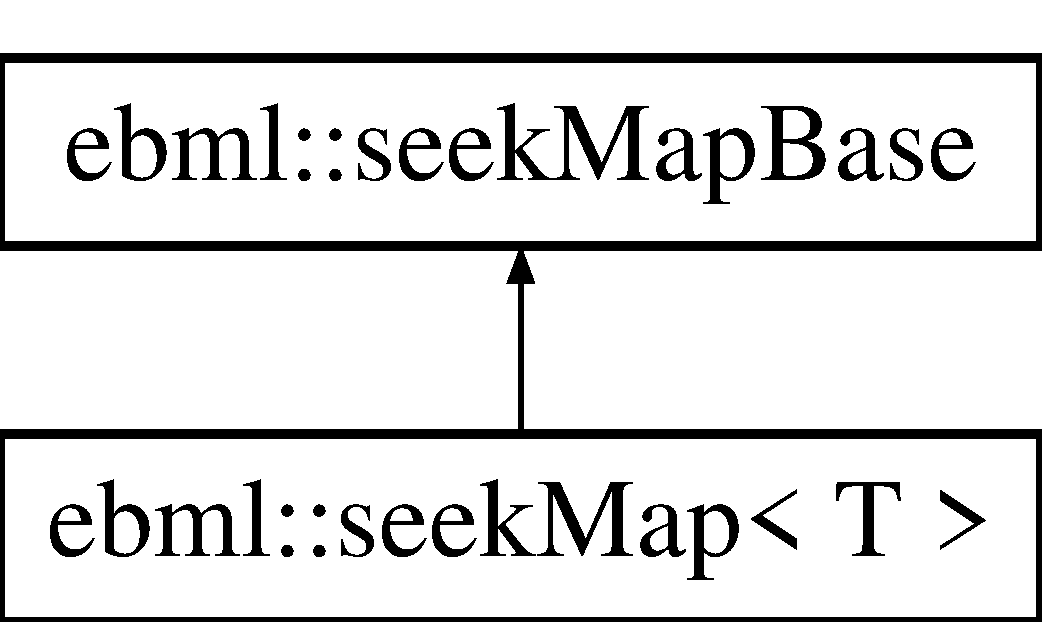
\includegraphics[height=2.000000cm]{classebml_1_1seekMapBase}
\end{center}
\end{figure}
\subsection*{Public Member Functions}
\begin{DoxyCompactItemize}
\item 
{\footnotesize template$<$typename T $>$ }\\\mbox{\hyperlink{classebml_1_1seekMap}{seek\+Map}}$<$ T $>$ \& \mbox{\hyperlink{classebml_1_1seekMapBase_ad313f809e97617d93b23191d03805492}{with\+Key\+Type}} ()
\item 
{\footnotesize template$<$typename T $>$ }\\const \mbox{\hyperlink{classebml_1_1seekMap}{seek\+Map}}$<$ T $>$ \& \mbox{\hyperlink{classebml_1_1seekMapBase_a174a7a2a9e40d0465b1c065e9549b5b4}{with\+Key\+Type}} () const
\item 
{\footnotesize template$<$typename T $>$ }\\\mbox{\hyperlink{classebml_1_1seekDataWithKey__t}{seek\+Data\+With\+Key\+\_\+t}}$<$ T $>$ $\ast$\& \mbox{\hyperlink{classebml_1_1seekMapBase_ac2f1f5151d43f5a9c04adc835fdc456f}{operator\mbox{[}$\,$\mbox{]}}} (const T \&)
\item 
{\footnotesize template$<$typename T $>$ }\\\mbox{\hyperlink{classebml_1_1seekDataWithKey__t}{seek\+Data\+With\+Key\+\_\+t}}$<$ T $>$ $\ast$\& \mbox{\hyperlink{classebml_1_1seekMapBase_a905bdf0b6e4dd19d7a2213391dcc3a0e}{at}} (const T \&)
\item 
{\footnotesize template$<$typename T $>$ }\\\mbox{\hyperlink{classebml_1_1seekDataWithKey__t}{seek\+Data\+With\+Key\+\_\+t}}$<$ T $>$ $\ast$const  \& \mbox{\hyperlink{classebml_1_1seekMapBase_addaab912ae0ef0fc525db52cbdb0aad5}{at}} (const T \&) const
\item 
{\footnotesize template$<$typename T $>$ }\\size\+\_\+t \mbox{\hyperlink{classebml_1_1seekMapBase_ac86fad8357bb9738ba022cfdb7f8e43c}{count}} (const T \&) const
\item 
{\footnotesize template$<$typename T $>$ }\\size\+\_\+t \mbox{\hyperlink{classebml_1_1seekMapBase_abeda7aee2215f0aec47e8ff0d607a902}{erase}} (const T \&)
\end{DoxyCompactItemize}


\subsection{Member Function Documentation}
\mbox{\Hypertarget{classebml_1_1seekMapBase_a905bdf0b6e4dd19d7a2213391dcc3a0e}\label{classebml_1_1seekMapBase_a905bdf0b6e4dd19d7a2213391dcc3a0e}} 
\index{ebml\+::seek\+Map\+Base@{ebml\+::seek\+Map\+Base}!at@{at}}
\index{at@{at}!ebml\+::seek\+Map\+Base@{ebml\+::seek\+Map\+Base}}
\subsubsection{\texorpdfstring{at()}{at()}\hspace{0.1cm}{\footnotesize\ttfamily [1/2]}}
{\footnotesize\ttfamily template$<$typename T $>$ \\
\mbox{\hyperlink{classebml_1_1seekDataWithKey__t}{seek\+Data\+With\+Key\+\_\+t}}$<$T$>$$\ast$\& ebml\+::seek\+Map\+Base\+::at (\begin{DoxyParamCaption}\item[{const T \&}]{ }\end{DoxyParamCaption})}

\mbox{\Hypertarget{classebml_1_1seekMapBase_addaab912ae0ef0fc525db52cbdb0aad5}\label{classebml_1_1seekMapBase_addaab912ae0ef0fc525db52cbdb0aad5}} 
\index{ebml\+::seek\+Map\+Base@{ebml\+::seek\+Map\+Base}!at@{at}}
\index{at@{at}!ebml\+::seek\+Map\+Base@{ebml\+::seek\+Map\+Base}}
\subsubsection{\texorpdfstring{at()}{at()}\hspace{0.1cm}{\footnotesize\ttfamily [2/2]}}
{\footnotesize\ttfamily template$<$typename T $>$ \\
\mbox{\hyperlink{classebml_1_1seekDataWithKey__t}{seek\+Data\+With\+Key\+\_\+t}}$<$T$>$$\ast$ const\& ebml\+::seek\+Map\+Base\+::at (\begin{DoxyParamCaption}\item[{const T \&}]{ }\end{DoxyParamCaption}) const}

\mbox{\Hypertarget{classebml_1_1seekMapBase_ac86fad8357bb9738ba022cfdb7f8e43c}\label{classebml_1_1seekMapBase_ac86fad8357bb9738ba022cfdb7f8e43c}} 
\index{ebml\+::seek\+Map\+Base@{ebml\+::seek\+Map\+Base}!count@{count}}
\index{count@{count}!ebml\+::seek\+Map\+Base@{ebml\+::seek\+Map\+Base}}
\subsubsection{\texorpdfstring{count()}{count()}}
{\footnotesize\ttfamily template$<$typename T $>$ \\
size\+\_\+t ebml\+::seek\+Map\+Base\+::count (\begin{DoxyParamCaption}\item[{const T \&}]{ }\end{DoxyParamCaption}) const}

\mbox{\Hypertarget{classebml_1_1seekMapBase_abeda7aee2215f0aec47e8ff0d607a902}\label{classebml_1_1seekMapBase_abeda7aee2215f0aec47e8ff0d607a902}} 
\index{ebml\+::seek\+Map\+Base@{ebml\+::seek\+Map\+Base}!erase@{erase}}
\index{erase@{erase}!ebml\+::seek\+Map\+Base@{ebml\+::seek\+Map\+Base}}
\subsubsection{\texorpdfstring{erase()}{erase()}}
{\footnotesize\ttfamily template$<$typename T $>$ \\
size\+\_\+t ebml\+::seek\+Map\+Base\+::erase (\begin{DoxyParamCaption}\item[{const T \&}]{ }\end{DoxyParamCaption})}

\mbox{\Hypertarget{classebml_1_1seekMapBase_ac2f1f5151d43f5a9c04adc835fdc456f}\label{classebml_1_1seekMapBase_ac2f1f5151d43f5a9c04adc835fdc456f}} 
\index{ebml\+::seek\+Map\+Base@{ebml\+::seek\+Map\+Base}!operator\mbox{[}\mbox{]}@{operator[]}}
\index{operator\mbox{[}\mbox{]}@{operator[]}!ebml\+::seek\+Map\+Base@{ebml\+::seek\+Map\+Base}}
\subsubsection{\texorpdfstring{operator[]()}{operator[]()}}
{\footnotesize\ttfamily template$<$typename T $>$ \\
\mbox{\hyperlink{classebml_1_1seekDataWithKey__t}{seek\+Data\+With\+Key\+\_\+t}}$<$T$>$$\ast$\& ebml\+::seek\+Map\+Base\+::operator\mbox{[}$\,$\mbox{]} (\begin{DoxyParamCaption}\item[{const T \&}]{ }\end{DoxyParamCaption})}

\mbox{\Hypertarget{classebml_1_1seekMapBase_ad313f809e97617d93b23191d03805492}\label{classebml_1_1seekMapBase_ad313f809e97617d93b23191d03805492}} 
\index{ebml\+::seek\+Map\+Base@{ebml\+::seek\+Map\+Base}!with\+Key\+Type@{with\+Key\+Type}}
\index{with\+Key\+Type@{with\+Key\+Type}!ebml\+::seek\+Map\+Base@{ebml\+::seek\+Map\+Base}}
\subsubsection{\texorpdfstring{with\+Key\+Type()}{withKeyType()}\hspace{0.1cm}{\footnotesize\ttfamily [1/2]}}
{\footnotesize\ttfamily template$<$typename T $>$ \\
\mbox{\hyperlink{classebml_1_1seekMap}{seek\+Map}}$<$T$>$\& ebml\+::seek\+Map\+Base\+::with\+Key\+Type (\begin{DoxyParamCaption}{ }\end{DoxyParamCaption})}

\mbox{\Hypertarget{classebml_1_1seekMapBase_a174a7a2a9e40d0465b1c065e9549b5b4}\label{classebml_1_1seekMapBase_a174a7a2a9e40d0465b1c065e9549b5b4}} 
\index{ebml\+::seek\+Map\+Base@{ebml\+::seek\+Map\+Base}!with\+Key\+Type@{with\+Key\+Type}}
\index{with\+Key\+Type@{with\+Key\+Type}!ebml\+::seek\+Map\+Base@{ebml\+::seek\+Map\+Base}}
\subsubsection{\texorpdfstring{with\+Key\+Type()}{withKeyType()}\hspace{0.1cm}{\footnotesize\ttfamily [2/2]}}
{\footnotesize\ttfamily template$<$typename T $>$ \\
const \mbox{\hyperlink{classebml_1_1seekMap}{seek\+Map}}$<$T$>$\& ebml\+::seek\+Map\+Base\+::with\+Key\+Type (\begin{DoxyParamCaption}{ }\end{DoxyParamCaption}) const}



The documentation for this class was generated from the following file\+:\begin{DoxyCompactItemize}
\item 
include/libebml\+\_\+ng/\mbox{\hyperlink{seekdata_8h}{seekdata.\+h}}\end{DoxyCompactItemize}

\hypertarget{structebml_1_1sizetree__t}{}\section{ebml\+:\+:sizetree\+\_\+t Struct Reference}
\label{structebml_1_1sizetree__t}\index{ebml\+::sizetree\+\_\+t@{ebml\+::sizetree\+\_\+t}}


{\ttfamily \#include $<$base.\+h$>$}

\subsection*{Public Member Functions}
\begin{DoxyCompactItemize}
\item 
\mbox{\hyperlink{structebml_1_1sizetree__t_ab6a2ee51cb1c9932e9db7c52f2a7caa1}{sizetree\+\_\+t}} ()
\item 
\mbox{\hyperlink{structebml_1_1sizetree__t_a742d446b695e31087692e335e6935ae2}{sizetree\+\_\+t}} (\mbox{\hyperlink{structebml_1_1sizetree__t}{sizetree\+\_\+t}} \&\&)
\item 
\mbox{\hyperlink{structebml_1_1sizetree__t_a41a80e1f9dbb5e031288a759f516abb5}{sizetree\+\_\+t}} (unsigned char \+\_\+ebml\+I\+D\+Width, unsigned char \+\_\+size\+Width, size\+\_\+t \+\_\+data\+Size)
\item 
\mbox{\hyperlink{structebml_1_1sizetree__t}{sizetree\+\_\+t}} \& \mbox{\hyperlink{structebml_1_1sizetree__t_a48e8c0b46c4dbf6a6aa467b3c8f5d896}{operator=}} (\mbox{\hyperlink{structebml_1_1sizetree__t}{sizetree\+\_\+t}} \&\&)
\item 
size\+\_\+t \mbox{\hyperlink{structebml_1_1sizetree__t_acbebda277c477cf6872985ee556bf329}{outer\+Size}} () const
\end{DoxyCompactItemize}
\subsection*{Public Attributes}
\begin{DoxyCompactItemize}
\item 
unsigned char \mbox{\hyperlink{structebml_1_1sizetree__t_a70bc5a5a11af951bf7ba77985677f499}{ebml\+I\+D\+Width}}
\item 
unsigned char \mbox{\hyperlink{structebml_1_1sizetree__t_a356c9d27fc953d49d010f4dc75438142}{size\+Width}}
\item 
size\+\_\+t \mbox{\hyperlink{structebml_1_1sizetree__t_ae6c505c09eae23cff574b42cccec1c30}{data\+Size}}
\item 
std\+::deque$<$ \mbox{\hyperlink{structebml_1_1sizetree__t}{sizetree\+\_\+t}} $>$ \mbox{\hyperlink{structebml_1_1sizetree__t_a5b13f1d6e607ba1b44be5ed3ccff549f}{children}}
\end{DoxyCompactItemize}


\subsection{Constructor \& Destructor Documentation}
\mbox{\Hypertarget{structebml_1_1sizetree__t_ab6a2ee51cb1c9932e9db7c52f2a7caa1}\label{structebml_1_1sizetree__t_ab6a2ee51cb1c9932e9db7c52f2a7caa1}} 
\index{ebml\+::sizetree\+\_\+t@{ebml\+::sizetree\+\_\+t}!sizetree\+\_\+t@{sizetree\+\_\+t}}
\index{sizetree\+\_\+t@{sizetree\+\_\+t}!ebml\+::sizetree\+\_\+t@{ebml\+::sizetree\+\_\+t}}
\subsubsection{\texorpdfstring{sizetree\+\_\+t()}{sizetree\_t()}\hspace{0.1cm}{\footnotesize\ttfamily [1/3]}}
{\footnotesize\ttfamily ebml\+::sizetree\+\_\+t\+::sizetree\+\_\+t (\begin{DoxyParamCaption}{ }\end{DoxyParamCaption})}

\mbox{\Hypertarget{structebml_1_1sizetree__t_a742d446b695e31087692e335e6935ae2}\label{structebml_1_1sizetree__t_a742d446b695e31087692e335e6935ae2}} 
\index{ebml\+::sizetree\+\_\+t@{ebml\+::sizetree\+\_\+t}!sizetree\+\_\+t@{sizetree\+\_\+t}}
\index{sizetree\+\_\+t@{sizetree\+\_\+t}!ebml\+::sizetree\+\_\+t@{ebml\+::sizetree\+\_\+t}}
\subsubsection{\texorpdfstring{sizetree\+\_\+t()}{sizetree\_t()}\hspace{0.1cm}{\footnotesize\ttfamily [2/3]}}
{\footnotesize\ttfamily ebml\+::sizetree\+\_\+t\+::sizetree\+\_\+t (\begin{DoxyParamCaption}\item[{\mbox{\hyperlink{structebml_1_1sizetree__t}{sizetree\+\_\+t}} \&\&}]{ }\end{DoxyParamCaption})}

\mbox{\Hypertarget{structebml_1_1sizetree__t_a41a80e1f9dbb5e031288a759f516abb5}\label{structebml_1_1sizetree__t_a41a80e1f9dbb5e031288a759f516abb5}} 
\index{ebml\+::sizetree\+\_\+t@{ebml\+::sizetree\+\_\+t}!sizetree\+\_\+t@{sizetree\+\_\+t}}
\index{sizetree\+\_\+t@{sizetree\+\_\+t}!ebml\+::sizetree\+\_\+t@{ebml\+::sizetree\+\_\+t}}
\subsubsection{\texorpdfstring{sizetree\+\_\+t()}{sizetree\_t()}\hspace{0.1cm}{\footnotesize\ttfamily [3/3]}}
{\footnotesize\ttfamily ebml\+::sizetree\+\_\+t\+::sizetree\+\_\+t (\begin{DoxyParamCaption}\item[{unsigned char}]{\+\_\+ebml\+I\+D\+Width,  }\item[{unsigned char}]{\+\_\+size\+Width,  }\item[{size\+\_\+t}]{\+\_\+data\+Size }\end{DoxyParamCaption})}



\subsection{Member Function Documentation}
\mbox{\Hypertarget{structebml_1_1sizetree__t_a48e8c0b46c4dbf6a6aa467b3c8f5d896}\label{structebml_1_1sizetree__t_a48e8c0b46c4dbf6a6aa467b3c8f5d896}} 
\index{ebml\+::sizetree\+\_\+t@{ebml\+::sizetree\+\_\+t}!operator=@{operator=}}
\index{operator=@{operator=}!ebml\+::sizetree\+\_\+t@{ebml\+::sizetree\+\_\+t}}
\subsubsection{\texorpdfstring{operator=()}{operator=()}}
{\footnotesize\ttfamily \mbox{\hyperlink{structebml_1_1sizetree__t}{sizetree\+\_\+t}}\& ebml\+::sizetree\+\_\+t\+::operator= (\begin{DoxyParamCaption}\item[{\mbox{\hyperlink{structebml_1_1sizetree__t}{sizetree\+\_\+t}} \&\&}]{ }\end{DoxyParamCaption})}

\mbox{\Hypertarget{structebml_1_1sizetree__t_acbebda277c477cf6872985ee556bf329}\label{structebml_1_1sizetree__t_acbebda277c477cf6872985ee556bf329}} 
\index{ebml\+::sizetree\+\_\+t@{ebml\+::sizetree\+\_\+t}!outer\+Size@{outer\+Size}}
\index{outer\+Size@{outer\+Size}!ebml\+::sizetree\+\_\+t@{ebml\+::sizetree\+\_\+t}}
\subsubsection{\texorpdfstring{outer\+Size()}{outerSize()}}
{\footnotesize\ttfamily size\+\_\+t ebml\+::sizetree\+\_\+t\+::outer\+Size (\begin{DoxyParamCaption}{ }\end{DoxyParamCaption}) const}



\subsection{Member Data Documentation}
\mbox{\Hypertarget{structebml_1_1sizetree__t_a5b13f1d6e607ba1b44be5ed3ccff549f}\label{structebml_1_1sizetree__t_a5b13f1d6e607ba1b44be5ed3ccff549f}} 
\index{ebml\+::sizetree\+\_\+t@{ebml\+::sizetree\+\_\+t}!children@{children}}
\index{children@{children}!ebml\+::sizetree\+\_\+t@{ebml\+::sizetree\+\_\+t}}
\subsubsection{\texorpdfstring{children}{children}}
{\footnotesize\ttfamily std\+::deque$<$\mbox{\hyperlink{structebml_1_1sizetree__t}{sizetree\+\_\+t}}$>$ ebml\+::sizetree\+\_\+t\+::children}

\mbox{\Hypertarget{structebml_1_1sizetree__t_ae6c505c09eae23cff574b42cccec1c30}\label{structebml_1_1sizetree__t_ae6c505c09eae23cff574b42cccec1c30}} 
\index{ebml\+::sizetree\+\_\+t@{ebml\+::sizetree\+\_\+t}!data\+Size@{data\+Size}}
\index{data\+Size@{data\+Size}!ebml\+::sizetree\+\_\+t@{ebml\+::sizetree\+\_\+t}}
\subsubsection{\texorpdfstring{data\+Size}{dataSize}}
{\footnotesize\ttfamily size\+\_\+t ebml\+::sizetree\+\_\+t\+::data\+Size}

\mbox{\Hypertarget{structebml_1_1sizetree__t_a70bc5a5a11af951bf7ba77985677f499}\label{structebml_1_1sizetree__t_a70bc5a5a11af951bf7ba77985677f499}} 
\index{ebml\+::sizetree\+\_\+t@{ebml\+::sizetree\+\_\+t}!ebml\+I\+D\+Width@{ebml\+I\+D\+Width}}
\index{ebml\+I\+D\+Width@{ebml\+I\+D\+Width}!ebml\+::sizetree\+\_\+t@{ebml\+::sizetree\+\_\+t}}
\subsubsection{\texorpdfstring{ebml\+I\+D\+Width}{ebmlIDWidth}}
{\footnotesize\ttfamily unsigned char ebml\+::sizetree\+\_\+t\+::ebml\+I\+D\+Width}

\mbox{\Hypertarget{structebml_1_1sizetree__t_a356c9d27fc953d49d010f4dc75438142}\label{structebml_1_1sizetree__t_a356c9d27fc953d49d010f4dc75438142}} 
\index{ebml\+::sizetree\+\_\+t@{ebml\+::sizetree\+\_\+t}!size\+Width@{size\+Width}}
\index{size\+Width@{size\+Width}!ebml\+::sizetree\+\_\+t@{ebml\+::sizetree\+\_\+t}}
\subsubsection{\texorpdfstring{size\+Width}{sizeWidth}}
{\footnotesize\ttfamily unsigned char ebml\+::sizetree\+\_\+t\+::size\+Width}



The documentation for this struct was generated from the following file\+:\begin{DoxyCompactItemize}
\item 
include/libebml\+\_\+ng/masterelement/\mbox{\hyperlink{base_8h}{base.\+h}}\end{DoxyCompactItemize}

\hypertarget{classebml_1_1slot__t}{}\section{ebml\+:\+:slot\+\_\+t Class Reference}
\label{classebml_1_1slot__t}\index{ebml\+::slot\+\_\+t@{ebml\+::slot\+\_\+t}}


{\ttfamily \#include $<$multislot.\+h$>$}

\subsection*{Classes}
\begin{DoxyCompactItemize}
\item 
class \mbox{\hyperlink{classebml_1_1slot__t_1_1iterator}{iterator}}
\end{DoxyCompactItemize}
\subsection*{Public Types}
\begin{DoxyCompactItemize}
\item 
typedef \mbox{\hyperlink{classebml_1_1const__slot__t_1_1iterator}{const\+\_\+slot\+\_\+t\+::iterator}} \mbox{\hyperlink{classebml_1_1slot__t_a035ab426d9062fc23e67d2b89f67ee84}{const\+\_\+iterator}}
\end{DoxyCompactItemize}
\subsection*{Public Member Functions}
\begin{DoxyCompactItemize}
\item 
\mbox{\hyperlink{classebml_1_1slot__t_a9eafcb1c7713718640339c65db36397d}{slot\+\_\+t}} (const \mbox{\hyperlink{classebml_1_1slot__t}{slot\+\_\+t}} \&)
\item 
\mbox{\hyperlink{classebml_1_1slot__t_a76551cd306d702fbce48749e32187fc9}{slot\+\_\+t}} (\mbox{\hyperlink{classebml_1_1slot__t}{slot\+\_\+t}} \&\&)
\item 
\mbox{\hyperlink{classebml_1_1slot__t}{slot\+\_\+t}} \& \mbox{\hyperlink{classebml_1_1slot__t_a691156a7c8cbe2ffadf29255e7e30615}{operator=}} (const \mbox{\hyperlink{classebml_1_1slot__t}{slot\+\_\+t}} \&)
\item 
\mbox{\hyperlink{classebml_1_1slot__t}{slot\+\_\+t}} \& \mbox{\hyperlink{classebml_1_1slot__t_a81a4b0f463d89955119880b9f15d1fd1}{operator=}} (\mbox{\hyperlink{classebml_1_1slot__t}{slot\+\_\+t}} \&\&)
\item 
\mbox{\hyperlink{classebml_1_1slot__t}{slot\+\_\+t}} \& \mbox{\hyperlink{classebml_1_1slot__t_a3978ca348f4b1a0c4b9f0287c394e1a4}{operator=}} (const \mbox{\hyperlink{namespaceebml_adad533b7705a16bb360fe56380c5e7be}{ebml\+Element\+\_\+sp}} \&)
\item 
\mbox{\hyperlink{classebml_1_1slot__t}{slot\+\_\+t}} \& \mbox{\hyperlink{classebml_1_1slot__t_ac3df4ed7828ec3b59cc608aa1be89ff3}{operator=}} (\mbox{\hyperlink{namespaceebml_adad533b7705a16bb360fe56380c5e7be}{ebml\+Element\+\_\+sp}} \&\&)
\item 
\mbox{\hyperlink{classebml_1_1slot__t_a89f3135580818ad0797c74baee65197d}{operator const ebml\+Element\+\_\+sp \&}} ()
\item 
\mbox{\hyperlink{classebml_1_1slot__t_aec1d933d5142acc72f3af01eb48d9353}{operator c\+\_\+ebml\+Element\+\_\+sp}} () const
\item 
\mbox{\hyperlink{classebml_1_1slot__t}{slot\+\_\+t}} \& \mbox{\hyperlink{classebml_1_1slot__t_a79517bf5358ba5c6f10a051a9073a340}{operator=}} (const \mbox{\hyperlink{namespaceebml_a1ddadd26791f273d851882653b9caf70}{ebml\+Element\+\_\+l}} \&)
\item 
\mbox{\hyperlink{classebml_1_1slot__t}{slot\+\_\+t}} \& \mbox{\hyperlink{classebml_1_1slot__t_a27b1914f5101516ef38491dcec55c30b}{operator=}} (\mbox{\hyperlink{namespaceebml_a1ddadd26791f273d851882653b9caf70}{ebml\+Element\+\_\+l}} \&\&)
\item 
\mbox{\hyperlink{classebml_1_1slot__t_ad350289e207fb6f5125b849d1174bb80}{operator const ebml\+Element\+\_\+l \&}} ()
\item 
\mbox{\hyperlink{classebml_1_1slot__t_abee3be5508e39066bd27923d9c138483}{operator c\+\_\+ebml\+Element\+\_\+l}} () const
\item 
\mbox{\hyperlink{classebml_1_1childSlot__t}{child\+Slot\+\_\+t}} \mbox{\hyperlink{classebml_1_1slot__t_a734f8cf3993a309a557557aca1cd6be8}{operator\mbox{[}$\,$\mbox{]}}} (size\+\_\+t)
\item 
\mbox{\hyperlink{classebml_1_1childSlot__t}{child\+Slot\+\_\+t}} \mbox{\hyperlink{classebml_1_1slot__t_abfa9697fbfa05ad723314497bdc7c299}{at}} (size\+\_\+t)
\item 
\mbox{\hyperlink{classebml_1_1childSlot__t}{child\+Slot\+\_\+t}} \mbox{\hyperlink{classebml_1_1slot__t_ad12308e65302012bfe30509c40e76174}{front}} ()
\item 
\mbox{\hyperlink{classebml_1_1childSlot__t}{child\+Slot\+\_\+t}} \mbox{\hyperlink{classebml_1_1slot__t_adc0fab024b3dd1a22e1ac27081ed1677}{back}} ()
\item 
\mbox{\hyperlink{classebml_1_1childSlot__t}{child\+Slot\+\_\+t}} \mbox{\hyperlink{classebml_1_1slot__t_acdbb11a14ce186aff8ebb95b98296afb}{push\+\_\+back}} (const \mbox{\hyperlink{namespaceebml_adad533b7705a16bb360fe56380c5e7be}{ebml\+Element\+\_\+sp}} \&)
\item 
\mbox{\hyperlink{classebml_1_1childSlot__t}{child\+Slot\+\_\+t}} \mbox{\hyperlink{classebml_1_1slot__t_acdfefb7ae413147ae5904d59d888d52d}{push\+\_\+back}} (\mbox{\hyperlink{namespaceebml_adad533b7705a16bb360fe56380c5e7be}{ebml\+Element\+\_\+sp}} \&\&)
\item 
\mbox{\hyperlink{namespaceebml_a2deef4e8071531b32e3533f1bf978917}{c\+\_\+ebml\+Element\+\_\+sp}} \mbox{\hyperlink{classebml_1_1slot__t_a553f97004880e160551be68ab05c33ce}{operator\mbox{[}$\,$\mbox{]}}} (size\+\_\+t) const
\item 
\mbox{\hyperlink{namespaceebml_a2deef4e8071531b32e3533f1bf978917}{c\+\_\+ebml\+Element\+\_\+sp}} \mbox{\hyperlink{classebml_1_1slot__t_acf1d704eae91fc410487421b80988f57}{at}} (size\+\_\+t) const
\item 
\mbox{\hyperlink{namespaceebml_a2deef4e8071531b32e3533f1bf978917}{c\+\_\+ebml\+Element\+\_\+sp}} \mbox{\hyperlink{classebml_1_1slot__t_ae7817a18a552f1399251c077dc6b65ad}{front}} () const
\item 
\mbox{\hyperlink{namespaceebml_a2deef4e8071531b32e3533f1bf978917}{c\+\_\+ebml\+Element\+\_\+sp}} \mbox{\hyperlink{classebml_1_1slot__t_ae9b2a7d37d5f8d71e97e973c9c708899}{back}} () const
\item 
\mbox{\hyperlink{classebml_1_1slot__t_1_1iterator}{iterator}} \mbox{\hyperlink{classebml_1_1slot__t_a590850d87ced3306465a19fa1c84bd47}{begin}} ()
\item 
\mbox{\hyperlink{classebml_1_1slot__t_1_1iterator}{iterator}} \mbox{\hyperlink{classebml_1_1slot__t_a47204fa4e7da5f36c97aeb36de78751d}{end}} ()
\item 
\mbox{\hyperlink{classebml_1_1slot__t_a035ab426d9062fc23e67d2b89f67ee84}{const\+\_\+iterator}} \mbox{\hyperlink{classebml_1_1slot__t_a36172913879365e6df9b9deabdad96e3}{cbegin}} () const
\item 
\mbox{\hyperlink{classebml_1_1slot__t_a035ab426d9062fc23e67d2b89f67ee84}{const\+\_\+iterator}} \mbox{\hyperlink{classebml_1_1slot__t_a4e6943c40ac9c311ce2a2b2c8284919c}{cend}} () const
\end{DoxyCompactItemize}
\subsection*{Protected Member Functions}
\begin{DoxyCompactItemize}
\item 
\mbox{\hyperlink{classebml_1_1slot__t_a9e43770cb5bc36f0cdbd1a9942d9844e}{slot\+\_\+t}} (const \mbox{\hyperlink{namespaceebml_adad533b7705a16bb360fe56380c5e7be}{ebml\+Element\+\_\+sp}} \&, \+\_\+slot\+\_\+t \&)
\end{DoxyCompactItemize}
\subsection*{Protected Attributes}
\begin{DoxyCompactItemize}
\item 
\mbox{\hyperlink{namespaceebml_a1e633eb51fcbe25caf953fd159171543}{ebml\+Multi\+Slot\+\_\+sp}} \mbox{\hyperlink{classebml_1_1slot__t_af18d868b3273a624355c01639673711b}{\+\_\+parent}}
\item 
\+\_\+slot\+\_\+t $\ast$ \mbox{\hyperlink{classebml_1_1slot__t_a0ae4e9259d6abf3697978fa71d120e94}{\+\_\+slot}}
\end{DoxyCompactItemize}
\subsection*{Friends}
\begin{DoxyCompactItemize}
\item 
class \mbox{\hyperlink{classebml_1_1slot__t_a4df98a34a57f946e69b766054b391d08}{const\+\_\+slot\+\_\+t}}
\item 
class \mbox{\hyperlink{classebml_1_1slot__t_a67171474c4da6cc8efe0c7fafefd2b2d}{iterator}}
\item 
class \mbox{\hyperlink{classebml_1_1slot__t_ab14eb6c5a125d7276a7b4b5b6573428b}{ebml\+Multi\+Slot}}
\end{DoxyCompactItemize}


\subsection{Member Typedef Documentation}
\mbox{\Hypertarget{classebml_1_1slot__t_a035ab426d9062fc23e67d2b89f67ee84}\label{classebml_1_1slot__t_a035ab426d9062fc23e67d2b89f67ee84}} 
\index{ebml\+::slot\+\_\+t@{ebml\+::slot\+\_\+t}!const\+\_\+iterator@{const\+\_\+iterator}}
\index{const\+\_\+iterator@{const\+\_\+iterator}!ebml\+::slot\+\_\+t@{ebml\+::slot\+\_\+t}}
\subsubsection{\texorpdfstring{const\+\_\+iterator}{const\_iterator}}
{\footnotesize\ttfamily typedef \mbox{\hyperlink{classebml_1_1const__slot__t_1_1iterator}{const\+\_\+slot\+\_\+t\+::iterator}} \mbox{\hyperlink{classebml_1_1slot__t_a035ab426d9062fc23e67d2b89f67ee84}{ebml\+::slot\+\_\+t\+::const\+\_\+iterator}}}



\subsection{Constructor \& Destructor Documentation}
\mbox{\Hypertarget{classebml_1_1slot__t_a9e43770cb5bc36f0cdbd1a9942d9844e}\label{classebml_1_1slot__t_a9e43770cb5bc36f0cdbd1a9942d9844e}} 
\index{ebml\+::slot\+\_\+t@{ebml\+::slot\+\_\+t}!slot\+\_\+t@{slot\+\_\+t}}
\index{slot\+\_\+t@{slot\+\_\+t}!ebml\+::slot\+\_\+t@{ebml\+::slot\+\_\+t}}
\subsubsection{\texorpdfstring{slot\+\_\+t()}{slot\_t()}\hspace{0.1cm}{\footnotesize\ttfamily [1/3]}}
{\footnotesize\ttfamily ebml\+::slot\+\_\+t\+::slot\+\_\+t (\begin{DoxyParamCaption}\item[{const \mbox{\hyperlink{namespaceebml_adad533b7705a16bb360fe56380c5e7be}{ebml\+Element\+\_\+sp}} \&}]{,  }\item[{\+\_\+slot\+\_\+t \&}]{ }\end{DoxyParamCaption})\hspace{0.3cm}{\ttfamily [protected]}}

\mbox{\Hypertarget{classebml_1_1slot__t_a9eafcb1c7713718640339c65db36397d}\label{classebml_1_1slot__t_a9eafcb1c7713718640339c65db36397d}} 
\index{ebml\+::slot\+\_\+t@{ebml\+::slot\+\_\+t}!slot\+\_\+t@{slot\+\_\+t}}
\index{slot\+\_\+t@{slot\+\_\+t}!ebml\+::slot\+\_\+t@{ebml\+::slot\+\_\+t}}
\subsubsection{\texorpdfstring{slot\+\_\+t()}{slot\_t()}\hspace{0.1cm}{\footnotesize\ttfamily [2/3]}}
{\footnotesize\ttfamily ebml\+::slot\+\_\+t\+::slot\+\_\+t (\begin{DoxyParamCaption}\item[{const \mbox{\hyperlink{classebml_1_1slot__t}{slot\+\_\+t}} \&}]{ }\end{DoxyParamCaption})}

\mbox{\Hypertarget{classebml_1_1slot__t_a76551cd306d702fbce48749e32187fc9}\label{classebml_1_1slot__t_a76551cd306d702fbce48749e32187fc9}} 
\index{ebml\+::slot\+\_\+t@{ebml\+::slot\+\_\+t}!slot\+\_\+t@{slot\+\_\+t}}
\index{slot\+\_\+t@{slot\+\_\+t}!ebml\+::slot\+\_\+t@{ebml\+::slot\+\_\+t}}
\subsubsection{\texorpdfstring{slot\+\_\+t()}{slot\_t()}\hspace{0.1cm}{\footnotesize\ttfamily [3/3]}}
{\footnotesize\ttfamily ebml\+::slot\+\_\+t\+::slot\+\_\+t (\begin{DoxyParamCaption}\item[{\mbox{\hyperlink{classebml_1_1slot__t}{slot\+\_\+t}} \&\&}]{ }\end{DoxyParamCaption})}



\subsection{Member Function Documentation}
\mbox{\Hypertarget{classebml_1_1slot__t_abfa9697fbfa05ad723314497bdc7c299}\label{classebml_1_1slot__t_abfa9697fbfa05ad723314497bdc7c299}} 
\index{ebml\+::slot\+\_\+t@{ebml\+::slot\+\_\+t}!at@{at}}
\index{at@{at}!ebml\+::slot\+\_\+t@{ebml\+::slot\+\_\+t}}
\subsubsection{\texorpdfstring{at()}{at()}\hspace{0.1cm}{\footnotesize\ttfamily [1/2]}}
{\footnotesize\ttfamily \mbox{\hyperlink{classebml_1_1childSlot__t}{child\+Slot\+\_\+t}} ebml\+::slot\+\_\+t\+::at (\begin{DoxyParamCaption}\item[{size\+\_\+t}]{ }\end{DoxyParamCaption})}

\mbox{\Hypertarget{classebml_1_1slot__t_acf1d704eae91fc410487421b80988f57}\label{classebml_1_1slot__t_acf1d704eae91fc410487421b80988f57}} 
\index{ebml\+::slot\+\_\+t@{ebml\+::slot\+\_\+t}!at@{at}}
\index{at@{at}!ebml\+::slot\+\_\+t@{ebml\+::slot\+\_\+t}}
\subsubsection{\texorpdfstring{at()}{at()}\hspace{0.1cm}{\footnotesize\ttfamily [2/2]}}
{\footnotesize\ttfamily \mbox{\hyperlink{namespaceebml_a2deef4e8071531b32e3533f1bf978917}{c\+\_\+ebml\+Element\+\_\+sp}} ebml\+::slot\+\_\+t\+::at (\begin{DoxyParamCaption}\item[{size\+\_\+t}]{ }\end{DoxyParamCaption}) const}

\mbox{\Hypertarget{classebml_1_1slot__t_adc0fab024b3dd1a22e1ac27081ed1677}\label{classebml_1_1slot__t_adc0fab024b3dd1a22e1ac27081ed1677}} 
\index{ebml\+::slot\+\_\+t@{ebml\+::slot\+\_\+t}!back@{back}}
\index{back@{back}!ebml\+::slot\+\_\+t@{ebml\+::slot\+\_\+t}}
\subsubsection{\texorpdfstring{back()}{back()}\hspace{0.1cm}{\footnotesize\ttfamily [1/2]}}
{\footnotesize\ttfamily \mbox{\hyperlink{classebml_1_1childSlot__t}{child\+Slot\+\_\+t}} ebml\+::slot\+\_\+t\+::back (\begin{DoxyParamCaption}{ }\end{DoxyParamCaption})}

\mbox{\Hypertarget{classebml_1_1slot__t_ae9b2a7d37d5f8d71e97e973c9c708899}\label{classebml_1_1slot__t_ae9b2a7d37d5f8d71e97e973c9c708899}} 
\index{ebml\+::slot\+\_\+t@{ebml\+::slot\+\_\+t}!back@{back}}
\index{back@{back}!ebml\+::slot\+\_\+t@{ebml\+::slot\+\_\+t}}
\subsubsection{\texorpdfstring{back()}{back()}\hspace{0.1cm}{\footnotesize\ttfamily [2/2]}}
{\footnotesize\ttfamily \mbox{\hyperlink{namespaceebml_a2deef4e8071531b32e3533f1bf978917}{c\+\_\+ebml\+Element\+\_\+sp}} ebml\+::slot\+\_\+t\+::back (\begin{DoxyParamCaption}{ }\end{DoxyParamCaption}) const}

\mbox{\Hypertarget{classebml_1_1slot__t_a590850d87ced3306465a19fa1c84bd47}\label{classebml_1_1slot__t_a590850d87ced3306465a19fa1c84bd47}} 
\index{ebml\+::slot\+\_\+t@{ebml\+::slot\+\_\+t}!begin@{begin}}
\index{begin@{begin}!ebml\+::slot\+\_\+t@{ebml\+::slot\+\_\+t}}
\subsubsection{\texorpdfstring{begin()}{begin()}}
{\footnotesize\ttfamily \mbox{\hyperlink{classebml_1_1slot__t_1_1iterator}{iterator}} ebml\+::slot\+\_\+t\+::begin (\begin{DoxyParamCaption}{ }\end{DoxyParamCaption})}

\mbox{\Hypertarget{classebml_1_1slot__t_a36172913879365e6df9b9deabdad96e3}\label{classebml_1_1slot__t_a36172913879365e6df9b9deabdad96e3}} 
\index{ebml\+::slot\+\_\+t@{ebml\+::slot\+\_\+t}!cbegin@{cbegin}}
\index{cbegin@{cbegin}!ebml\+::slot\+\_\+t@{ebml\+::slot\+\_\+t}}
\subsubsection{\texorpdfstring{cbegin()}{cbegin()}}
{\footnotesize\ttfamily \mbox{\hyperlink{classebml_1_1slot__t_a035ab426d9062fc23e67d2b89f67ee84}{const\+\_\+iterator}} ebml\+::slot\+\_\+t\+::cbegin (\begin{DoxyParamCaption}{ }\end{DoxyParamCaption}) const}

\mbox{\Hypertarget{classebml_1_1slot__t_a4e6943c40ac9c311ce2a2b2c8284919c}\label{classebml_1_1slot__t_a4e6943c40ac9c311ce2a2b2c8284919c}} 
\index{ebml\+::slot\+\_\+t@{ebml\+::slot\+\_\+t}!cend@{cend}}
\index{cend@{cend}!ebml\+::slot\+\_\+t@{ebml\+::slot\+\_\+t}}
\subsubsection{\texorpdfstring{cend()}{cend()}}
{\footnotesize\ttfamily \mbox{\hyperlink{classebml_1_1slot__t_a035ab426d9062fc23e67d2b89f67ee84}{const\+\_\+iterator}} ebml\+::slot\+\_\+t\+::cend (\begin{DoxyParamCaption}{ }\end{DoxyParamCaption}) const}

\mbox{\Hypertarget{classebml_1_1slot__t_a47204fa4e7da5f36c97aeb36de78751d}\label{classebml_1_1slot__t_a47204fa4e7da5f36c97aeb36de78751d}} 
\index{ebml\+::slot\+\_\+t@{ebml\+::slot\+\_\+t}!end@{end}}
\index{end@{end}!ebml\+::slot\+\_\+t@{ebml\+::slot\+\_\+t}}
\subsubsection{\texorpdfstring{end()}{end()}}
{\footnotesize\ttfamily \mbox{\hyperlink{classebml_1_1slot__t_1_1iterator}{iterator}} ebml\+::slot\+\_\+t\+::end (\begin{DoxyParamCaption}{ }\end{DoxyParamCaption})}

\mbox{\Hypertarget{classebml_1_1slot__t_ad12308e65302012bfe30509c40e76174}\label{classebml_1_1slot__t_ad12308e65302012bfe30509c40e76174}} 
\index{ebml\+::slot\+\_\+t@{ebml\+::slot\+\_\+t}!front@{front}}
\index{front@{front}!ebml\+::slot\+\_\+t@{ebml\+::slot\+\_\+t}}
\subsubsection{\texorpdfstring{front()}{front()}\hspace{0.1cm}{\footnotesize\ttfamily [1/2]}}
{\footnotesize\ttfamily \mbox{\hyperlink{classebml_1_1childSlot__t}{child\+Slot\+\_\+t}} ebml\+::slot\+\_\+t\+::front (\begin{DoxyParamCaption}{ }\end{DoxyParamCaption})}

\mbox{\Hypertarget{classebml_1_1slot__t_ae7817a18a552f1399251c077dc6b65ad}\label{classebml_1_1slot__t_ae7817a18a552f1399251c077dc6b65ad}} 
\index{ebml\+::slot\+\_\+t@{ebml\+::slot\+\_\+t}!front@{front}}
\index{front@{front}!ebml\+::slot\+\_\+t@{ebml\+::slot\+\_\+t}}
\subsubsection{\texorpdfstring{front()}{front()}\hspace{0.1cm}{\footnotesize\ttfamily [2/2]}}
{\footnotesize\ttfamily \mbox{\hyperlink{namespaceebml_a2deef4e8071531b32e3533f1bf978917}{c\+\_\+ebml\+Element\+\_\+sp}} ebml\+::slot\+\_\+t\+::front (\begin{DoxyParamCaption}{ }\end{DoxyParamCaption}) const}

\mbox{\Hypertarget{classebml_1_1slot__t_abee3be5508e39066bd27923d9c138483}\label{classebml_1_1slot__t_abee3be5508e39066bd27923d9c138483}} 
\index{ebml\+::slot\+\_\+t@{ebml\+::slot\+\_\+t}!operator c\+\_\+ebml\+Element\+\_\+l@{operator c\+\_\+ebml\+Element\+\_\+l}}
\index{operator c\+\_\+ebml\+Element\+\_\+l@{operator c\+\_\+ebml\+Element\+\_\+l}!ebml\+::slot\+\_\+t@{ebml\+::slot\+\_\+t}}
\subsubsection{\texorpdfstring{operator c\+\_\+ebml\+Element\+\_\+l()}{operator c\_ebmlElement\_l()}}
{\footnotesize\ttfamily ebml\+::slot\+\_\+t\+::operator \mbox{\hyperlink{classebml_1_1c__ebmlElement__l}{c\+\_\+ebml\+Element\+\_\+l}} (\begin{DoxyParamCaption}{ }\end{DoxyParamCaption}) const}

\mbox{\Hypertarget{classebml_1_1slot__t_aec1d933d5142acc72f3af01eb48d9353}\label{classebml_1_1slot__t_aec1d933d5142acc72f3af01eb48d9353}} 
\index{ebml\+::slot\+\_\+t@{ebml\+::slot\+\_\+t}!operator c\+\_\+ebml\+Element\+\_\+sp@{operator c\+\_\+ebml\+Element\+\_\+sp}}
\index{operator c\+\_\+ebml\+Element\+\_\+sp@{operator c\+\_\+ebml\+Element\+\_\+sp}!ebml\+::slot\+\_\+t@{ebml\+::slot\+\_\+t}}
\subsubsection{\texorpdfstring{operator c\+\_\+ebml\+Element\+\_\+sp()}{operator c\_ebmlElement\_sp()}}
{\footnotesize\ttfamily ebml\+::slot\+\_\+t\+::operator \mbox{\hyperlink{namespaceebml_a2deef4e8071531b32e3533f1bf978917}{c\+\_\+ebml\+Element\+\_\+sp}} (\begin{DoxyParamCaption}{ }\end{DoxyParamCaption}) const}

\mbox{\Hypertarget{classebml_1_1slot__t_ad350289e207fb6f5125b849d1174bb80}\label{classebml_1_1slot__t_ad350289e207fb6f5125b849d1174bb80}} 
\index{ebml\+::slot\+\_\+t@{ebml\+::slot\+\_\+t}!operator const ebml\+Element\+\_\+l \&@{operator const ebml\+Element\+\_\+l \&}}
\index{operator const ebml\+Element\+\_\+l \&@{operator const ebml\+Element\+\_\+l \&}!ebml\+::slot\+\_\+t@{ebml\+::slot\+\_\+t}}
\subsubsection{\texorpdfstring{operator const ebml\+Element\+\_\+l \&()}{operator const ebmlElement\_l \&()}}
{\footnotesize\ttfamily ebml\+::slot\+\_\+t\+::operator const \mbox{\hyperlink{namespaceebml_a1ddadd26791f273d851882653b9caf70}{ebml\+Element\+\_\+l}} \& (\begin{DoxyParamCaption}{ }\end{DoxyParamCaption})}

\mbox{\Hypertarget{classebml_1_1slot__t_a89f3135580818ad0797c74baee65197d}\label{classebml_1_1slot__t_a89f3135580818ad0797c74baee65197d}} 
\index{ebml\+::slot\+\_\+t@{ebml\+::slot\+\_\+t}!operator const ebml\+Element\+\_\+sp \&@{operator const ebml\+Element\+\_\+sp \&}}
\index{operator const ebml\+Element\+\_\+sp \&@{operator const ebml\+Element\+\_\+sp \&}!ebml\+::slot\+\_\+t@{ebml\+::slot\+\_\+t}}
\subsubsection{\texorpdfstring{operator const ebml\+Element\+\_\+sp \&()}{operator const ebmlElement\_sp \&()}}
{\footnotesize\ttfamily ebml\+::slot\+\_\+t\+::operator const \mbox{\hyperlink{namespaceebml_adad533b7705a16bb360fe56380c5e7be}{ebml\+Element\+\_\+sp}} \& (\begin{DoxyParamCaption}{ }\end{DoxyParamCaption})}

\mbox{\Hypertarget{classebml_1_1slot__t_a691156a7c8cbe2ffadf29255e7e30615}\label{classebml_1_1slot__t_a691156a7c8cbe2ffadf29255e7e30615}} 
\index{ebml\+::slot\+\_\+t@{ebml\+::slot\+\_\+t}!operator=@{operator=}}
\index{operator=@{operator=}!ebml\+::slot\+\_\+t@{ebml\+::slot\+\_\+t}}
\subsubsection{\texorpdfstring{operator=()}{operator=()}\hspace{0.1cm}{\footnotesize\ttfamily [1/6]}}
{\footnotesize\ttfamily \mbox{\hyperlink{classebml_1_1slot__t}{slot\+\_\+t}}\& ebml\+::slot\+\_\+t\+::operator= (\begin{DoxyParamCaption}\item[{const \mbox{\hyperlink{classebml_1_1slot__t}{slot\+\_\+t}} \&}]{ }\end{DoxyParamCaption})}

\mbox{\Hypertarget{classebml_1_1slot__t_a81a4b0f463d89955119880b9f15d1fd1}\label{classebml_1_1slot__t_a81a4b0f463d89955119880b9f15d1fd1}} 
\index{ebml\+::slot\+\_\+t@{ebml\+::slot\+\_\+t}!operator=@{operator=}}
\index{operator=@{operator=}!ebml\+::slot\+\_\+t@{ebml\+::slot\+\_\+t}}
\subsubsection{\texorpdfstring{operator=()}{operator=()}\hspace{0.1cm}{\footnotesize\ttfamily [2/6]}}
{\footnotesize\ttfamily \mbox{\hyperlink{classebml_1_1slot__t}{slot\+\_\+t}}\& ebml\+::slot\+\_\+t\+::operator= (\begin{DoxyParamCaption}\item[{\mbox{\hyperlink{classebml_1_1slot__t}{slot\+\_\+t}} \&\&}]{ }\end{DoxyParamCaption})}

\mbox{\Hypertarget{classebml_1_1slot__t_a3978ca348f4b1a0c4b9f0287c394e1a4}\label{classebml_1_1slot__t_a3978ca348f4b1a0c4b9f0287c394e1a4}} 
\index{ebml\+::slot\+\_\+t@{ebml\+::slot\+\_\+t}!operator=@{operator=}}
\index{operator=@{operator=}!ebml\+::slot\+\_\+t@{ebml\+::slot\+\_\+t}}
\subsubsection{\texorpdfstring{operator=()}{operator=()}\hspace{0.1cm}{\footnotesize\ttfamily [3/6]}}
{\footnotesize\ttfamily \mbox{\hyperlink{classebml_1_1slot__t}{slot\+\_\+t}}\& ebml\+::slot\+\_\+t\+::operator= (\begin{DoxyParamCaption}\item[{const \mbox{\hyperlink{namespaceebml_adad533b7705a16bb360fe56380c5e7be}{ebml\+Element\+\_\+sp}} \&}]{ }\end{DoxyParamCaption})}

\mbox{\Hypertarget{classebml_1_1slot__t_ac3df4ed7828ec3b59cc608aa1be89ff3}\label{classebml_1_1slot__t_ac3df4ed7828ec3b59cc608aa1be89ff3}} 
\index{ebml\+::slot\+\_\+t@{ebml\+::slot\+\_\+t}!operator=@{operator=}}
\index{operator=@{operator=}!ebml\+::slot\+\_\+t@{ebml\+::slot\+\_\+t}}
\subsubsection{\texorpdfstring{operator=()}{operator=()}\hspace{0.1cm}{\footnotesize\ttfamily [4/6]}}
{\footnotesize\ttfamily \mbox{\hyperlink{classebml_1_1slot__t}{slot\+\_\+t}}\& ebml\+::slot\+\_\+t\+::operator= (\begin{DoxyParamCaption}\item[{\mbox{\hyperlink{namespaceebml_adad533b7705a16bb360fe56380c5e7be}{ebml\+Element\+\_\+sp}} \&\&}]{ }\end{DoxyParamCaption})}

\mbox{\Hypertarget{classebml_1_1slot__t_a79517bf5358ba5c6f10a051a9073a340}\label{classebml_1_1slot__t_a79517bf5358ba5c6f10a051a9073a340}} 
\index{ebml\+::slot\+\_\+t@{ebml\+::slot\+\_\+t}!operator=@{operator=}}
\index{operator=@{operator=}!ebml\+::slot\+\_\+t@{ebml\+::slot\+\_\+t}}
\subsubsection{\texorpdfstring{operator=()}{operator=()}\hspace{0.1cm}{\footnotesize\ttfamily [5/6]}}
{\footnotesize\ttfamily \mbox{\hyperlink{classebml_1_1slot__t}{slot\+\_\+t}}\& ebml\+::slot\+\_\+t\+::operator= (\begin{DoxyParamCaption}\item[{const \mbox{\hyperlink{namespaceebml_a1ddadd26791f273d851882653b9caf70}{ebml\+Element\+\_\+l}} \&}]{ }\end{DoxyParamCaption})}

\mbox{\Hypertarget{classebml_1_1slot__t_a27b1914f5101516ef38491dcec55c30b}\label{classebml_1_1slot__t_a27b1914f5101516ef38491dcec55c30b}} 
\index{ebml\+::slot\+\_\+t@{ebml\+::slot\+\_\+t}!operator=@{operator=}}
\index{operator=@{operator=}!ebml\+::slot\+\_\+t@{ebml\+::slot\+\_\+t}}
\subsubsection{\texorpdfstring{operator=()}{operator=()}\hspace{0.1cm}{\footnotesize\ttfamily [6/6]}}
{\footnotesize\ttfamily \mbox{\hyperlink{classebml_1_1slot__t}{slot\+\_\+t}}\& ebml\+::slot\+\_\+t\+::operator= (\begin{DoxyParamCaption}\item[{\mbox{\hyperlink{namespaceebml_a1ddadd26791f273d851882653b9caf70}{ebml\+Element\+\_\+l}} \&\&}]{ }\end{DoxyParamCaption})}

\mbox{\Hypertarget{classebml_1_1slot__t_a734f8cf3993a309a557557aca1cd6be8}\label{classebml_1_1slot__t_a734f8cf3993a309a557557aca1cd6be8}} 
\index{ebml\+::slot\+\_\+t@{ebml\+::slot\+\_\+t}!operator\mbox{[}\mbox{]}@{operator[]}}
\index{operator\mbox{[}\mbox{]}@{operator[]}!ebml\+::slot\+\_\+t@{ebml\+::slot\+\_\+t}}
\subsubsection{\texorpdfstring{operator[]()}{operator[]()}\hspace{0.1cm}{\footnotesize\ttfamily [1/2]}}
{\footnotesize\ttfamily \mbox{\hyperlink{classebml_1_1childSlot__t}{child\+Slot\+\_\+t}} ebml\+::slot\+\_\+t\+::operator\mbox{[}$\,$\mbox{]} (\begin{DoxyParamCaption}\item[{size\+\_\+t}]{ }\end{DoxyParamCaption})}

\mbox{\Hypertarget{classebml_1_1slot__t_a553f97004880e160551be68ab05c33ce}\label{classebml_1_1slot__t_a553f97004880e160551be68ab05c33ce}} 
\index{ebml\+::slot\+\_\+t@{ebml\+::slot\+\_\+t}!operator\mbox{[}\mbox{]}@{operator[]}}
\index{operator\mbox{[}\mbox{]}@{operator[]}!ebml\+::slot\+\_\+t@{ebml\+::slot\+\_\+t}}
\subsubsection{\texorpdfstring{operator[]()}{operator[]()}\hspace{0.1cm}{\footnotesize\ttfamily [2/2]}}
{\footnotesize\ttfamily \mbox{\hyperlink{namespaceebml_a2deef4e8071531b32e3533f1bf978917}{c\+\_\+ebml\+Element\+\_\+sp}} ebml\+::slot\+\_\+t\+::operator\mbox{[}$\,$\mbox{]} (\begin{DoxyParamCaption}\item[{size\+\_\+t}]{ }\end{DoxyParamCaption}) const}

\mbox{\Hypertarget{classebml_1_1slot__t_acdbb11a14ce186aff8ebb95b98296afb}\label{classebml_1_1slot__t_acdbb11a14ce186aff8ebb95b98296afb}} 
\index{ebml\+::slot\+\_\+t@{ebml\+::slot\+\_\+t}!push\+\_\+back@{push\+\_\+back}}
\index{push\+\_\+back@{push\+\_\+back}!ebml\+::slot\+\_\+t@{ebml\+::slot\+\_\+t}}
\subsubsection{\texorpdfstring{push\+\_\+back()}{push\_back()}\hspace{0.1cm}{\footnotesize\ttfamily [1/2]}}
{\footnotesize\ttfamily \mbox{\hyperlink{classebml_1_1childSlot__t}{child\+Slot\+\_\+t}} ebml\+::slot\+\_\+t\+::push\+\_\+back (\begin{DoxyParamCaption}\item[{const \mbox{\hyperlink{namespaceebml_adad533b7705a16bb360fe56380c5e7be}{ebml\+Element\+\_\+sp}} \&}]{ }\end{DoxyParamCaption})}

\mbox{\Hypertarget{classebml_1_1slot__t_acdfefb7ae413147ae5904d59d888d52d}\label{classebml_1_1slot__t_acdfefb7ae413147ae5904d59d888d52d}} 
\index{ebml\+::slot\+\_\+t@{ebml\+::slot\+\_\+t}!push\+\_\+back@{push\+\_\+back}}
\index{push\+\_\+back@{push\+\_\+back}!ebml\+::slot\+\_\+t@{ebml\+::slot\+\_\+t}}
\subsubsection{\texorpdfstring{push\+\_\+back()}{push\_back()}\hspace{0.1cm}{\footnotesize\ttfamily [2/2]}}
{\footnotesize\ttfamily \mbox{\hyperlink{classebml_1_1childSlot__t}{child\+Slot\+\_\+t}} ebml\+::slot\+\_\+t\+::push\+\_\+back (\begin{DoxyParamCaption}\item[{\mbox{\hyperlink{namespaceebml_adad533b7705a16bb360fe56380c5e7be}{ebml\+Element\+\_\+sp}} \&\&}]{ }\end{DoxyParamCaption})}



\subsection{Friends And Related Function Documentation}
\mbox{\Hypertarget{classebml_1_1slot__t_a4df98a34a57f946e69b766054b391d08}\label{classebml_1_1slot__t_a4df98a34a57f946e69b766054b391d08}} 
\index{ebml\+::slot\+\_\+t@{ebml\+::slot\+\_\+t}!const\+\_\+slot\+\_\+t@{const\+\_\+slot\+\_\+t}}
\index{const\+\_\+slot\+\_\+t@{const\+\_\+slot\+\_\+t}!ebml\+::slot\+\_\+t@{ebml\+::slot\+\_\+t}}
\subsubsection{\texorpdfstring{const\+\_\+slot\+\_\+t}{const\_slot\_t}}
{\footnotesize\ttfamily friend class \mbox{\hyperlink{classebml_1_1const__slot__t}{const\+\_\+slot\+\_\+t}}\hspace{0.3cm}{\ttfamily [friend]}}

\mbox{\Hypertarget{classebml_1_1slot__t_ab14eb6c5a125d7276a7b4b5b6573428b}\label{classebml_1_1slot__t_ab14eb6c5a125d7276a7b4b5b6573428b}} 
\index{ebml\+::slot\+\_\+t@{ebml\+::slot\+\_\+t}!ebml\+Multi\+Slot@{ebml\+Multi\+Slot}}
\index{ebml\+Multi\+Slot@{ebml\+Multi\+Slot}!ebml\+::slot\+\_\+t@{ebml\+::slot\+\_\+t}}
\subsubsection{\texorpdfstring{ebml\+Multi\+Slot}{ebmlMultiSlot}}
{\footnotesize\ttfamily friend class \mbox{\hyperlink{classebml_1_1ebmlMultiSlot}{ebml\+Multi\+Slot}}\hspace{0.3cm}{\ttfamily [friend]}}

\mbox{\Hypertarget{classebml_1_1slot__t_a67171474c4da6cc8efe0c7fafefd2b2d}\label{classebml_1_1slot__t_a67171474c4da6cc8efe0c7fafefd2b2d}} 
\index{ebml\+::slot\+\_\+t@{ebml\+::slot\+\_\+t}!iterator@{iterator}}
\index{iterator@{iterator}!ebml\+::slot\+\_\+t@{ebml\+::slot\+\_\+t}}
\subsubsection{\texorpdfstring{iterator}{iterator}}
{\footnotesize\ttfamily friend class \mbox{\hyperlink{classebml_1_1slot__t_1_1iterator}{iterator}}\hspace{0.3cm}{\ttfamily [friend]}}



\subsection{Member Data Documentation}
\mbox{\Hypertarget{classebml_1_1slot__t_af18d868b3273a624355c01639673711b}\label{classebml_1_1slot__t_af18d868b3273a624355c01639673711b}} 
\index{ebml\+::slot\+\_\+t@{ebml\+::slot\+\_\+t}!\+\_\+parent@{\+\_\+parent}}
\index{\+\_\+parent@{\+\_\+parent}!ebml\+::slot\+\_\+t@{ebml\+::slot\+\_\+t}}
\subsubsection{\texorpdfstring{\+\_\+parent}{\_parent}}
{\footnotesize\ttfamily \mbox{\hyperlink{namespaceebml_a1e633eb51fcbe25caf953fd159171543}{ebml\+Multi\+Slot\+\_\+sp}} ebml\+::slot\+\_\+t\+::\+\_\+parent\hspace{0.3cm}{\ttfamily [protected]}}

\mbox{\Hypertarget{classebml_1_1slot__t_a0ae4e9259d6abf3697978fa71d120e94}\label{classebml_1_1slot__t_a0ae4e9259d6abf3697978fa71d120e94}} 
\index{ebml\+::slot\+\_\+t@{ebml\+::slot\+\_\+t}!\+\_\+slot@{\+\_\+slot}}
\index{\+\_\+slot@{\+\_\+slot}!ebml\+::slot\+\_\+t@{ebml\+::slot\+\_\+t}}
\subsubsection{\texorpdfstring{\+\_\+slot}{\_slot}}
{\footnotesize\ttfamily \+\_\+slot\+\_\+t$\ast$ ebml\+::slot\+\_\+t\+::\+\_\+slot\hspace{0.3cm}{\ttfamily [protected]}}



The documentation for this class was generated from the following file\+:\begin{DoxyCompactItemize}
\item 
include/libebml\+\_\+ng/masterelement/\mbox{\hyperlink{multislot_8h}{multislot.\+h}}\end{DoxyCompactItemize}

\hypertarget{classebml_1_1slotArg__t}{}\section{ebml\+:\+:slot\+Arg\+\_\+t Class Reference}
\label{classebml_1_1slotArg__t}\index{ebml\+::slot\+Arg\+\_\+t@{ebml\+::slot\+Arg\+\_\+t}}


{\ttfamily \#include $<$multislot.\+h$>$}

\subsection*{Public Member Functions}
\begin{DoxyCompactItemize}
\item 
\mbox{\hyperlink{classebml_1_1slotArg__t_a59249e5f6cf0f643d4ebea7bc5f01e53}{slot\+Arg\+\_\+t}} ()
\item 
\mbox{\hyperlink{classebml_1_1slotArg__t_a591c64b34980557575356624d41f1dfa}{slot\+Arg\+\_\+t}} (const std\+::nullptr\+\_\+t \&)
\item 
\mbox{\hyperlink{classebml_1_1slotArg__t_a6d0298f32f02bb42259aecaf109c06f1}{slot\+Arg\+\_\+t}} (const \mbox{\hyperlink{namespaceebml_adad533b7705a16bb360fe56380c5e7be}{ebml\+Element\+\_\+sp}} \&)
\item 
\mbox{\hyperlink{classebml_1_1slotArg__t_a51d5c0e7d0fa1c08aa838b2dcf0000e0}{slot\+Arg\+\_\+t}} (\mbox{\hyperlink{namespaceebml_adad533b7705a16bb360fe56380c5e7be}{ebml\+Element\+\_\+sp}} \&\&)
\item 
\mbox{\hyperlink{classebml_1_1slotArg__t_a96b4367cbf3107c56fc9bcb5ef72a203}{slot\+Arg\+\_\+t}} (const \mbox{\hyperlink{namespaceebml_a1ddadd26791f273d851882653b9caf70}{ebml\+Element\+\_\+l}} \&)
\item 
\mbox{\hyperlink{classebml_1_1slotArg__t_a77b50a5a4f95f700be0b7aacb7117a79}{slot\+Arg\+\_\+t}} (\mbox{\hyperlink{namespaceebml_a1ddadd26791f273d851882653b9caf70}{ebml\+Element\+\_\+l}} \&\&)
\item 
\mbox{\hyperlink{classebml_1_1slotArg__t_a41a7e21e1780fc1965d1c9ec1cf50c35}{slot\+Arg\+\_\+t}} (const \mbox{\hyperlink{classebml_1_1slotArg__t}{slot\+Arg\+\_\+t}} \&)
\item 
\mbox{\hyperlink{classebml_1_1slotArg__t_a557c93afda9fcf328c28ecfc3877790e}{slot\+Arg\+\_\+t}} (\mbox{\hyperlink{classebml_1_1slotArg__t}{slot\+Arg\+\_\+t}} \&\&)
\item 
\mbox{\hyperlink{classebml_1_1slotArg__t}{slot\+Arg\+\_\+t}} \& \mbox{\hyperlink{classebml_1_1slotArg__t_a1a584ff973b655fad2bc8cc4dadbe859}{operator=}} (const \mbox{\hyperlink{classebml_1_1slotArg__t}{slot\+Arg\+\_\+t}} \&)
\item 
\mbox{\hyperlink{classebml_1_1slotArg__t}{slot\+Arg\+\_\+t}} \& \mbox{\hyperlink{classebml_1_1slotArg__t_aeff50ae008a8002833d3baa52f22fd17}{operator=}} (\mbox{\hyperlink{classebml_1_1slotArg__t}{slot\+Arg\+\_\+t}} \&\&)
\item 
\mbox{\hyperlink{classebml_1_1slotArg__t}{slot\+Arg\+\_\+t}} \& \mbox{\hyperlink{classebml_1_1slotArg__t_a01e1399671dde26089dfd42528357de5}{operator=}} (const \mbox{\hyperlink{namespaceebml_adad533b7705a16bb360fe56380c5e7be}{ebml\+Element\+\_\+sp}} \&)
\item 
\mbox{\hyperlink{classebml_1_1slotArg__t}{slot\+Arg\+\_\+t}} \& \mbox{\hyperlink{classebml_1_1slotArg__t_a9f8040d5b36f81615059a9a8d41739de}{operator=}} (\mbox{\hyperlink{namespaceebml_adad533b7705a16bb360fe56380c5e7be}{ebml\+Element\+\_\+sp}} \&\&)
\item 
\mbox{\hyperlink{classebml_1_1slotArg__t}{slot\+Arg\+\_\+t}} \& \mbox{\hyperlink{classebml_1_1slotArg__t_a54036af9209665fea3f02b8c2822aea5}{operator=}} (const \mbox{\hyperlink{namespaceebml_a1ddadd26791f273d851882653b9caf70}{ebml\+Element\+\_\+l}} \&)
\item 
\mbox{\hyperlink{classebml_1_1slotArg__t}{slot\+Arg\+\_\+t}} \& \mbox{\hyperlink{classebml_1_1slotArg__t_ae7d90c0e339c51fc5c5422453dcc3d9b}{operator=}} (\mbox{\hyperlink{namespaceebml_a1ddadd26791f273d851882653b9caf70}{ebml\+Element\+\_\+l}} \&\&)
\item 
bool \mbox{\hyperlink{classebml_1_1slotArg__t_a4ad4a3ec18db484c30c4da595732c115}{multi}} () const
\item 
\mbox{\hyperlink{classebml_1_1slotArg__t_ad0da9203bac5e560fb2fc5314f75a49a}{operator ebml\+Element\+\_\+sp \&}} ()
\item 
\mbox{\hyperlink{classebml_1_1slotArg__t_aac0c66b2f856c712e6d5bb1c82764af1}{operator const ebml\+Element\+\_\+sp \&}} () const
\item 
\mbox{\hyperlink{classebml_1_1slotArg__t_a004e63b5e9bbe78b613c09c7b7e814d1}{operator ebml\+Element\+\_\+l \&}} ()
\item 
\mbox{\hyperlink{classebml_1_1slotArg__t_a21decdc348045decac411a84ecc4e6e6}{operator const ebml\+Element\+\_\+l \&}} () const
\item 
\mbox{\hyperlink{classebml_1_1slotArg__t_aa141995137dafb51f5041f04688ed276}{$\sim$slot\+Arg\+\_\+t}} ()
\end{DoxyCompactItemize}


\subsection{Constructor \& Destructor Documentation}
\mbox{\Hypertarget{classebml_1_1slotArg__t_a59249e5f6cf0f643d4ebea7bc5f01e53}\label{classebml_1_1slotArg__t_a59249e5f6cf0f643d4ebea7bc5f01e53}} 
\index{ebml\+::slot\+Arg\+\_\+t@{ebml\+::slot\+Arg\+\_\+t}!slot\+Arg\+\_\+t@{slot\+Arg\+\_\+t}}
\index{slot\+Arg\+\_\+t@{slot\+Arg\+\_\+t}!ebml\+::slot\+Arg\+\_\+t@{ebml\+::slot\+Arg\+\_\+t}}
\subsubsection{\texorpdfstring{slot\+Arg\+\_\+t()}{slotArg\_t()}\hspace{0.1cm}{\footnotesize\ttfamily [1/8]}}
{\footnotesize\ttfamily ebml\+::slot\+Arg\+\_\+t\+::slot\+Arg\+\_\+t (\begin{DoxyParamCaption}{ }\end{DoxyParamCaption})}

\mbox{\Hypertarget{classebml_1_1slotArg__t_a591c64b34980557575356624d41f1dfa}\label{classebml_1_1slotArg__t_a591c64b34980557575356624d41f1dfa}} 
\index{ebml\+::slot\+Arg\+\_\+t@{ebml\+::slot\+Arg\+\_\+t}!slot\+Arg\+\_\+t@{slot\+Arg\+\_\+t}}
\index{slot\+Arg\+\_\+t@{slot\+Arg\+\_\+t}!ebml\+::slot\+Arg\+\_\+t@{ebml\+::slot\+Arg\+\_\+t}}
\subsubsection{\texorpdfstring{slot\+Arg\+\_\+t()}{slotArg\_t()}\hspace{0.1cm}{\footnotesize\ttfamily [2/8]}}
{\footnotesize\ttfamily ebml\+::slot\+Arg\+\_\+t\+::slot\+Arg\+\_\+t (\begin{DoxyParamCaption}\item[{const std\+::nullptr\+\_\+t \&}]{ }\end{DoxyParamCaption})}

\mbox{\Hypertarget{classebml_1_1slotArg__t_a6d0298f32f02bb42259aecaf109c06f1}\label{classebml_1_1slotArg__t_a6d0298f32f02bb42259aecaf109c06f1}} 
\index{ebml\+::slot\+Arg\+\_\+t@{ebml\+::slot\+Arg\+\_\+t}!slot\+Arg\+\_\+t@{slot\+Arg\+\_\+t}}
\index{slot\+Arg\+\_\+t@{slot\+Arg\+\_\+t}!ebml\+::slot\+Arg\+\_\+t@{ebml\+::slot\+Arg\+\_\+t}}
\subsubsection{\texorpdfstring{slot\+Arg\+\_\+t()}{slotArg\_t()}\hspace{0.1cm}{\footnotesize\ttfamily [3/8]}}
{\footnotesize\ttfamily ebml\+::slot\+Arg\+\_\+t\+::slot\+Arg\+\_\+t (\begin{DoxyParamCaption}\item[{const \mbox{\hyperlink{namespaceebml_adad533b7705a16bb360fe56380c5e7be}{ebml\+Element\+\_\+sp}} \&}]{ }\end{DoxyParamCaption})}

\mbox{\Hypertarget{classebml_1_1slotArg__t_a51d5c0e7d0fa1c08aa838b2dcf0000e0}\label{classebml_1_1slotArg__t_a51d5c0e7d0fa1c08aa838b2dcf0000e0}} 
\index{ebml\+::slot\+Arg\+\_\+t@{ebml\+::slot\+Arg\+\_\+t}!slot\+Arg\+\_\+t@{slot\+Arg\+\_\+t}}
\index{slot\+Arg\+\_\+t@{slot\+Arg\+\_\+t}!ebml\+::slot\+Arg\+\_\+t@{ebml\+::slot\+Arg\+\_\+t}}
\subsubsection{\texorpdfstring{slot\+Arg\+\_\+t()}{slotArg\_t()}\hspace{0.1cm}{\footnotesize\ttfamily [4/8]}}
{\footnotesize\ttfamily ebml\+::slot\+Arg\+\_\+t\+::slot\+Arg\+\_\+t (\begin{DoxyParamCaption}\item[{\mbox{\hyperlink{namespaceebml_adad533b7705a16bb360fe56380c5e7be}{ebml\+Element\+\_\+sp}} \&\&}]{ }\end{DoxyParamCaption})}

\mbox{\Hypertarget{classebml_1_1slotArg__t_a96b4367cbf3107c56fc9bcb5ef72a203}\label{classebml_1_1slotArg__t_a96b4367cbf3107c56fc9bcb5ef72a203}} 
\index{ebml\+::slot\+Arg\+\_\+t@{ebml\+::slot\+Arg\+\_\+t}!slot\+Arg\+\_\+t@{slot\+Arg\+\_\+t}}
\index{slot\+Arg\+\_\+t@{slot\+Arg\+\_\+t}!ebml\+::slot\+Arg\+\_\+t@{ebml\+::slot\+Arg\+\_\+t}}
\subsubsection{\texorpdfstring{slot\+Arg\+\_\+t()}{slotArg\_t()}\hspace{0.1cm}{\footnotesize\ttfamily [5/8]}}
{\footnotesize\ttfamily ebml\+::slot\+Arg\+\_\+t\+::slot\+Arg\+\_\+t (\begin{DoxyParamCaption}\item[{const \mbox{\hyperlink{namespaceebml_a1ddadd26791f273d851882653b9caf70}{ebml\+Element\+\_\+l}} \&}]{ }\end{DoxyParamCaption})}

\mbox{\Hypertarget{classebml_1_1slotArg__t_a77b50a5a4f95f700be0b7aacb7117a79}\label{classebml_1_1slotArg__t_a77b50a5a4f95f700be0b7aacb7117a79}} 
\index{ebml\+::slot\+Arg\+\_\+t@{ebml\+::slot\+Arg\+\_\+t}!slot\+Arg\+\_\+t@{slot\+Arg\+\_\+t}}
\index{slot\+Arg\+\_\+t@{slot\+Arg\+\_\+t}!ebml\+::slot\+Arg\+\_\+t@{ebml\+::slot\+Arg\+\_\+t}}
\subsubsection{\texorpdfstring{slot\+Arg\+\_\+t()}{slotArg\_t()}\hspace{0.1cm}{\footnotesize\ttfamily [6/8]}}
{\footnotesize\ttfamily ebml\+::slot\+Arg\+\_\+t\+::slot\+Arg\+\_\+t (\begin{DoxyParamCaption}\item[{\mbox{\hyperlink{namespaceebml_a1ddadd26791f273d851882653b9caf70}{ebml\+Element\+\_\+l}} \&\&}]{ }\end{DoxyParamCaption})}

\mbox{\Hypertarget{classebml_1_1slotArg__t_a41a7e21e1780fc1965d1c9ec1cf50c35}\label{classebml_1_1slotArg__t_a41a7e21e1780fc1965d1c9ec1cf50c35}} 
\index{ebml\+::slot\+Arg\+\_\+t@{ebml\+::slot\+Arg\+\_\+t}!slot\+Arg\+\_\+t@{slot\+Arg\+\_\+t}}
\index{slot\+Arg\+\_\+t@{slot\+Arg\+\_\+t}!ebml\+::slot\+Arg\+\_\+t@{ebml\+::slot\+Arg\+\_\+t}}
\subsubsection{\texorpdfstring{slot\+Arg\+\_\+t()}{slotArg\_t()}\hspace{0.1cm}{\footnotesize\ttfamily [7/8]}}
{\footnotesize\ttfamily ebml\+::slot\+Arg\+\_\+t\+::slot\+Arg\+\_\+t (\begin{DoxyParamCaption}\item[{const \mbox{\hyperlink{classebml_1_1slotArg__t}{slot\+Arg\+\_\+t}} \&}]{ }\end{DoxyParamCaption})}

\mbox{\Hypertarget{classebml_1_1slotArg__t_a557c93afda9fcf328c28ecfc3877790e}\label{classebml_1_1slotArg__t_a557c93afda9fcf328c28ecfc3877790e}} 
\index{ebml\+::slot\+Arg\+\_\+t@{ebml\+::slot\+Arg\+\_\+t}!slot\+Arg\+\_\+t@{slot\+Arg\+\_\+t}}
\index{slot\+Arg\+\_\+t@{slot\+Arg\+\_\+t}!ebml\+::slot\+Arg\+\_\+t@{ebml\+::slot\+Arg\+\_\+t}}
\subsubsection{\texorpdfstring{slot\+Arg\+\_\+t()}{slotArg\_t()}\hspace{0.1cm}{\footnotesize\ttfamily [8/8]}}
{\footnotesize\ttfamily ebml\+::slot\+Arg\+\_\+t\+::slot\+Arg\+\_\+t (\begin{DoxyParamCaption}\item[{\mbox{\hyperlink{classebml_1_1slotArg__t}{slot\+Arg\+\_\+t}} \&\&}]{ }\end{DoxyParamCaption})}

\mbox{\Hypertarget{classebml_1_1slotArg__t_aa141995137dafb51f5041f04688ed276}\label{classebml_1_1slotArg__t_aa141995137dafb51f5041f04688ed276}} 
\index{ebml\+::slot\+Arg\+\_\+t@{ebml\+::slot\+Arg\+\_\+t}!````~slot\+Arg\+\_\+t@{$\sim$slot\+Arg\+\_\+t}}
\index{````~slot\+Arg\+\_\+t@{$\sim$slot\+Arg\+\_\+t}!ebml\+::slot\+Arg\+\_\+t@{ebml\+::slot\+Arg\+\_\+t}}
\subsubsection{\texorpdfstring{$\sim$slot\+Arg\+\_\+t()}{~slotArg\_t()}}
{\footnotesize\ttfamily ebml\+::slot\+Arg\+\_\+t\+::$\sim$slot\+Arg\+\_\+t (\begin{DoxyParamCaption}{ }\end{DoxyParamCaption})}



\subsection{Member Function Documentation}
\mbox{\Hypertarget{classebml_1_1slotArg__t_a4ad4a3ec18db484c30c4da595732c115}\label{classebml_1_1slotArg__t_a4ad4a3ec18db484c30c4da595732c115}} 
\index{ebml\+::slot\+Arg\+\_\+t@{ebml\+::slot\+Arg\+\_\+t}!multi@{multi}}
\index{multi@{multi}!ebml\+::slot\+Arg\+\_\+t@{ebml\+::slot\+Arg\+\_\+t}}
\subsubsection{\texorpdfstring{multi()}{multi()}}
{\footnotesize\ttfamily bool ebml\+::slot\+Arg\+\_\+t\+::multi (\begin{DoxyParamCaption}{ }\end{DoxyParamCaption}) const}

\mbox{\Hypertarget{classebml_1_1slotArg__t_a21decdc348045decac411a84ecc4e6e6}\label{classebml_1_1slotArg__t_a21decdc348045decac411a84ecc4e6e6}} 
\index{ebml\+::slot\+Arg\+\_\+t@{ebml\+::slot\+Arg\+\_\+t}!operator const ebml\+Element\+\_\+l \&@{operator const ebml\+Element\+\_\+l \&}}
\index{operator const ebml\+Element\+\_\+l \&@{operator const ebml\+Element\+\_\+l \&}!ebml\+::slot\+Arg\+\_\+t@{ebml\+::slot\+Arg\+\_\+t}}
\subsubsection{\texorpdfstring{operator const ebml\+Element\+\_\+l \&()}{operator const ebmlElement\_l \&()}}
{\footnotesize\ttfamily ebml\+::slot\+Arg\+\_\+t\+::operator const \mbox{\hyperlink{namespaceebml_a1ddadd26791f273d851882653b9caf70}{ebml\+Element\+\_\+l}} \& (\begin{DoxyParamCaption}{ }\end{DoxyParamCaption}) const}

\mbox{\Hypertarget{classebml_1_1slotArg__t_aac0c66b2f856c712e6d5bb1c82764af1}\label{classebml_1_1slotArg__t_aac0c66b2f856c712e6d5bb1c82764af1}} 
\index{ebml\+::slot\+Arg\+\_\+t@{ebml\+::slot\+Arg\+\_\+t}!operator const ebml\+Element\+\_\+sp \&@{operator const ebml\+Element\+\_\+sp \&}}
\index{operator const ebml\+Element\+\_\+sp \&@{operator const ebml\+Element\+\_\+sp \&}!ebml\+::slot\+Arg\+\_\+t@{ebml\+::slot\+Arg\+\_\+t}}
\subsubsection{\texorpdfstring{operator const ebml\+Element\+\_\+sp \&()}{operator const ebmlElement\_sp \&()}}
{\footnotesize\ttfamily ebml\+::slot\+Arg\+\_\+t\+::operator const \mbox{\hyperlink{namespaceebml_adad533b7705a16bb360fe56380c5e7be}{ebml\+Element\+\_\+sp}} \& (\begin{DoxyParamCaption}{ }\end{DoxyParamCaption}) const}

\mbox{\Hypertarget{classebml_1_1slotArg__t_a004e63b5e9bbe78b613c09c7b7e814d1}\label{classebml_1_1slotArg__t_a004e63b5e9bbe78b613c09c7b7e814d1}} 
\index{ebml\+::slot\+Arg\+\_\+t@{ebml\+::slot\+Arg\+\_\+t}!operator ebml\+Element\+\_\+l \&@{operator ebml\+Element\+\_\+l \&}}
\index{operator ebml\+Element\+\_\+l \&@{operator ebml\+Element\+\_\+l \&}!ebml\+::slot\+Arg\+\_\+t@{ebml\+::slot\+Arg\+\_\+t}}
\subsubsection{\texorpdfstring{operator ebml\+Element\+\_\+l \&()}{operator ebmlElement\_l \&()}}
{\footnotesize\ttfamily ebml\+::slot\+Arg\+\_\+t\+::operator \mbox{\hyperlink{namespaceebml_a1ddadd26791f273d851882653b9caf70}{ebml\+Element\+\_\+l}} \& (\begin{DoxyParamCaption}{ }\end{DoxyParamCaption})}

\mbox{\Hypertarget{classebml_1_1slotArg__t_ad0da9203bac5e560fb2fc5314f75a49a}\label{classebml_1_1slotArg__t_ad0da9203bac5e560fb2fc5314f75a49a}} 
\index{ebml\+::slot\+Arg\+\_\+t@{ebml\+::slot\+Arg\+\_\+t}!operator ebml\+Element\+\_\+sp \&@{operator ebml\+Element\+\_\+sp \&}}
\index{operator ebml\+Element\+\_\+sp \&@{operator ebml\+Element\+\_\+sp \&}!ebml\+::slot\+Arg\+\_\+t@{ebml\+::slot\+Arg\+\_\+t}}
\subsubsection{\texorpdfstring{operator ebml\+Element\+\_\+sp \&()}{operator ebmlElement\_sp \&()}}
{\footnotesize\ttfamily ebml\+::slot\+Arg\+\_\+t\+::operator \mbox{\hyperlink{namespaceebml_adad533b7705a16bb360fe56380c5e7be}{ebml\+Element\+\_\+sp}} \& (\begin{DoxyParamCaption}{ }\end{DoxyParamCaption})}

\mbox{\Hypertarget{classebml_1_1slotArg__t_a1a584ff973b655fad2bc8cc4dadbe859}\label{classebml_1_1slotArg__t_a1a584ff973b655fad2bc8cc4dadbe859}} 
\index{ebml\+::slot\+Arg\+\_\+t@{ebml\+::slot\+Arg\+\_\+t}!operator=@{operator=}}
\index{operator=@{operator=}!ebml\+::slot\+Arg\+\_\+t@{ebml\+::slot\+Arg\+\_\+t}}
\subsubsection{\texorpdfstring{operator=()}{operator=()}\hspace{0.1cm}{\footnotesize\ttfamily [1/6]}}
{\footnotesize\ttfamily \mbox{\hyperlink{classebml_1_1slotArg__t}{slot\+Arg\+\_\+t}}\& ebml\+::slot\+Arg\+\_\+t\+::operator= (\begin{DoxyParamCaption}\item[{const \mbox{\hyperlink{classebml_1_1slotArg__t}{slot\+Arg\+\_\+t}} \&}]{ }\end{DoxyParamCaption})}

\mbox{\Hypertarget{classebml_1_1slotArg__t_aeff50ae008a8002833d3baa52f22fd17}\label{classebml_1_1slotArg__t_aeff50ae008a8002833d3baa52f22fd17}} 
\index{ebml\+::slot\+Arg\+\_\+t@{ebml\+::slot\+Arg\+\_\+t}!operator=@{operator=}}
\index{operator=@{operator=}!ebml\+::slot\+Arg\+\_\+t@{ebml\+::slot\+Arg\+\_\+t}}
\subsubsection{\texorpdfstring{operator=()}{operator=()}\hspace{0.1cm}{\footnotesize\ttfamily [2/6]}}
{\footnotesize\ttfamily \mbox{\hyperlink{classebml_1_1slotArg__t}{slot\+Arg\+\_\+t}}\& ebml\+::slot\+Arg\+\_\+t\+::operator= (\begin{DoxyParamCaption}\item[{\mbox{\hyperlink{classebml_1_1slotArg__t}{slot\+Arg\+\_\+t}} \&\&}]{ }\end{DoxyParamCaption})}

\mbox{\Hypertarget{classebml_1_1slotArg__t_a01e1399671dde26089dfd42528357de5}\label{classebml_1_1slotArg__t_a01e1399671dde26089dfd42528357de5}} 
\index{ebml\+::slot\+Arg\+\_\+t@{ebml\+::slot\+Arg\+\_\+t}!operator=@{operator=}}
\index{operator=@{operator=}!ebml\+::slot\+Arg\+\_\+t@{ebml\+::slot\+Arg\+\_\+t}}
\subsubsection{\texorpdfstring{operator=()}{operator=()}\hspace{0.1cm}{\footnotesize\ttfamily [3/6]}}
{\footnotesize\ttfamily \mbox{\hyperlink{classebml_1_1slotArg__t}{slot\+Arg\+\_\+t}}\& ebml\+::slot\+Arg\+\_\+t\+::operator= (\begin{DoxyParamCaption}\item[{const \mbox{\hyperlink{namespaceebml_adad533b7705a16bb360fe56380c5e7be}{ebml\+Element\+\_\+sp}} \&}]{ }\end{DoxyParamCaption})}

\mbox{\Hypertarget{classebml_1_1slotArg__t_a9f8040d5b36f81615059a9a8d41739de}\label{classebml_1_1slotArg__t_a9f8040d5b36f81615059a9a8d41739de}} 
\index{ebml\+::slot\+Arg\+\_\+t@{ebml\+::slot\+Arg\+\_\+t}!operator=@{operator=}}
\index{operator=@{operator=}!ebml\+::slot\+Arg\+\_\+t@{ebml\+::slot\+Arg\+\_\+t}}
\subsubsection{\texorpdfstring{operator=()}{operator=()}\hspace{0.1cm}{\footnotesize\ttfamily [4/6]}}
{\footnotesize\ttfamily \mbox{\hyperlink{classebml_1_1slotArg__t}{slot\+Arg\+\_\+t}}\& ebml\+::slot\+Arg\+\_\+t\+::operator= (\begin{DoxyParamCaption}\item[{\mbox{\hyperlink{namespaceebml_adad533b7705a16bb360fe56380c5e7be}{ebml\+Element\+\_\+sp}} \&\&}]{ }\end{DoxyParamCaption})}

\mbox{\Hypertarget{classebml_1_1slotArg__t_a54036af9209665fea3f02b8c2822aea5}\label{classebml_1_1slotArg__t_a54036af9209665fea3f02b8c2822aea5}} 
\index{ebml\+::slot\+Arg\+\_\+t@{ebml\+::slot\+Arg\+\_\+t}!operator=@{operator=}}
\index{operator=@{operator=}!ebml\+::slot\+Arg\+\_\+t@{ebml\+::slot\+Arg\+\_\+t}}
\subsubsection{\texorpdfstring{operator=()}{operator=()}\hspace{0.1cm}{\footnotesize\ttfamily [5/6]}}
{\footnotesize\ttfamily \mbox{\hyperlink{classebml_1_1slotArg__t}{slot\+Arg\+\_\+t}}\& ebml\+::slot\+Arg\+\_\+t\+::operator= (\begin{DoxyParamCaption}\item[{const \mbox{\hyperlink{namespaceebml_a1ddadd26791f273d851882653b9caf70}{ebml\+Element\+\_\+l}} \&}]{ }\end{DoxyParamCaption})}

\mbox{\Hypertarget{classebml_1_1slotArg__t_ae7d90c0e339c51fc5c5422453dcc3d9b}\label{classebml_1_1slotArg__t_ae7d90c0e339c51fc5c5422453dcc3d9b}} 
\index{ebml\+::slot\+Arg\+\_\+t@{ebml\+::slot\+Arg\+\_\+t}!operator=@{operator=}}
\index{operator=@{operator=}!ebml\+::slot\+Arg\+\_\+t@{ebml\+::slot\+Arg\+\_\+t}}
\subsubsection{\texorpdfstring{operator=()}{operator=()}\hspace{0.1cm}{\footnotesize\ttfamily [6/6]}}
{\footnotesize\ttfamily \mbox{\hyperlink{classebml_1_1slotArg__t}{slot\+Arg\+\_\+t}}\& ebml\+::slot\+Arg\+\_\+t\+::operator= (\begin{DoxyParamCaption}\item[{\mbox{\hyperlink{namespaceebml_a1ddadd26791f273d851882653b9caf70}{ebml\+Element\+\_\+l}} \&\&}]{ }\end{DoxyParamCaption})}



\subsection{Member Data Documentation}
\mbox{\Hypertarget{classebml_1_1slotArg__t_a325527b79851e58d33d7b9bbc1a28a67}\label{classebml_1_1slotArg__t_a325527b79851e58d33d7b9bbc1a28a67}} 
\index{ebml\+::slot\+Arg\+\_\+t@{ebml\+::slot\+Arg\+\_\+t}!elem@{elem}}
\index{elem@{elem}!ebml\+::slot\+Arg\+\_\+t@{ebml\+::slot\+Arg\+\_\+t}}
\subsubsection{\texorpdfstring{elem}{elem}}
{\footnotesize\ttfamily \mbox{\hyperlink{namespaceebml_adad533b7705a16bb360fe56380c5e7be}{ebml\+Element\+\_\+sp}} ebml\+::slot\+Arg\+\_\+t\+::elem}

\mbox{\Hypertarget{classebml_1_1slotArg__t_aa7536b9a47e616fb677d57e2bba570ba}\label{classebml_1_1slotArg__t_aa7536b9a47e616fb677d57e2bba570ba}} 
\index{ebml\+::slot\+Arg\+\_\+t@{ebml\+::slot\+Arg\+\_\+t}!elems@{elems}}
\index{elems@{elems}!ebml\+::slot\+Arg\+\_\+t@{ebml\+::slot\+Arg\+\_\+t}}
\subsubsection{\texorpdfstring{elems}{elems}}
{\footnotesize\ttfamily \mbox{\hyperlink{namespaceebml_a1ddadd26791f273d851882653b9caf70}{ebml\+Element\+\_\+l}} ebml\+::slot\+Arg\+\_\+t\+::elems}



The documentation for this class was generated from the following file\+:\begin{DoxyCompactItemize}
\item 
include/libebml\+\_\+ng/masterelement/\mbox{\hyperlink{multislot_8h}{multislot.\+h}}\end{DoxyCompactItemize}

\hypertarget{classebml_1_1slotSpec__t}{}\section{ebml\+:\+:slot\+Spec\+\_\+t Class Reference}
\label{classebml_1_1slotSpec__t}\index{ebml\+::slot\+Spec\+\_\+t@{ebml\+::slot\+Spec\+\_\+t}}


{\ttfamily \#include $<$multislot.\+h$>$}

\subsection*{Public Member Functions}
\begin{DoxyCompactItemize}
\item 
\mbox{\hyperlink{classebml_1_1slotSpec__t_a28a3cf34f3ab54176feac825ec132c9e}{slot\+Spec\+\_\+t}} ()
\item 
\mbox{\hyperlink{classebml_1_1slotSpec__t_a1d4e4264361ead0bccae5b28c7ba275b}{slot\+Spec\+\_\+t}} (const std\+::string \&, const \mbox{\hyperlink{namespaceebml_abf07998998c284c9be3f76b5d9e192e1}{child\+Class\+Spec\+Arg\+\_\+l}} \&, bool multielem=false)
\item 
\mbox{\hyperlink{classebml_1_1slotSpec__t_a98310fdebfa88812dcceaec3af20fe4b}{slot\+Spec\+\_\+t}} (const \mbox{\hyperlink{classebml_1_1slotSpec__t}{slot\+Spec\+\_\+t}} \&)
\item 
\mbox{\hyperlink{classebml_1_1slotSpec__t_acb5cb8f607dae2ec56efbc700a763759}{slot\+Spec\+\_\+t}} (\mbox{\hyperlink{classebml_1_1slotSpec__t}{slot\+Spec\+\_\+t}} \&\&)
\item 
\mbox{\hyperlink{classebml_1_1slotSpec__t_a8cf105dfb5bd9d77d88e306223f62a61}{$\sim$slot\+Spec\+\_\+t}} ()
\item 
\mbox{\hyperlink{classebml_1_1slotSpec__t}{slot\+Spec\+\_\+t}} \& \mbox{\hyperlink{classebml_1_1slotSpec__t_a46053c168b61bbc61c2125d3375d4e63}{operator=}} (const \mbox{\hyperlink{classebml_1_1slotSpec__t}{slot\+Spec\+\_\+t}} \&)
\item 
\mbox{\hyperlink{classebml_1_1slotSpec__t}{slot\+Spec\+\_\+t}} \& \mbox{\hyperlink{classebml_1_1slotSpec__t_aebedb39b17caaedb754dc14854fae54a}{operator=}} (\mbox{\hyperlink{classebml_1_1slotSpec__t}{slot\+Spec\+\_\+t}} \&\&)
\item 
const \mbox{\hyperlink{classebml_1_1childClassSpec__t}{child\+Class\+Spec\+\_\+t}} \& \mbox{\hyperlink{classebml_1_1slotSpec__t_ab0b0bb9fa4174f49d4cfa0d3b756b337}{child\+Classes}} () const
\item 
bool \mbox{\hyperlink{classebml_1_1slotSpec__t_a2216622e5df326773cc2854a2b638208}{multi}} () const
\end{DoxyCompactItemize}
\subsection*{Public Attributes}
\begin{DoxyCompactItemize}
\item 
std\+::string \mbox{\hyperlink{classebml_1_1slotSpec__t_ab9a69de9a5c4a33b900e3e127a21b4e3}{name}}
\end{DoxyCompactItemize}
\subsection*{Protected Attributes}
\begin{DoxyCompactItemize}
\item 
\mbox{\hyperlink{classebml_1_1childClassSpec__t}{child\+Class\+Spec\+\_\+t}} \mbox{\hyperlink{classebml_1_1slotSpec__t_af1be82ab2c44da470febb4a8a8aa9f2a}{\+\_\+child\+Classes}}
\item 
bool \mbox{\hyperlink{classebml_1_1slotSpec__t_a9cec2fe8084092d36d14ae101bbef2df}{\+\_\+multi}}
\end{DoxyCompactItemize}
\subsection*{Friends}
\begin{DoxyCompactItemize}
\item 
class \mbox{\hyperlink{classebml_1_1slotSpec__t_a03124469c35c80a29b81b969706999df}{\+\_\+slot\+\_\+t}}
\item 
class \mbox{\hyperlink{classebml_1_1slotSpec__t_a229e8a019ffa3d8ab84c711635badcd1}{ebml\+Multi\+Slot\+Class}}
\end{DoxyCompactItemize}


\subsection{Constructor \& Destructor Documentation}
\mbox{\Hypertarget{classebml_1_1slotSpec__t_a28a3cf34f3ab54176feac825ec132c9e}\label{classebml_1_1slotSpec__t_a28a3cf34f3ab54176feac825ec132c9e}} 
\index{ebml\+::slot\+Spec\+\_\+t@{ebml\+::slot\+Spec\+\_\+t}!slot\+Spec\+\_\+t@{slot\+Spec\+\_\+t}}
\index{slot\+Spec\+\_\+t@{slot\+Spec\+\_\+t}!ebml\+::slot\+Spec\+\_\+t@{ebml\+::slot\+Spec\+\_\+t}}
\subsubsection{\texorpdfstring{slot\+Spec\+\_\+t()}{slotSpec\_t()}\hspace{0.1cm}{\footnotesize\ttfamily [1/4]}}
{\footnotesize\ttfamily ebml\+::slot\+Spec\+\_\+t\+::slot\+Spec\+\_\+t (\begin{DoxyParamCaption}{ }\end{DoxyParamCaption})}

\mbox{\Hypertarget{classebml_1_1slotSpec__t_a1d4e4264361ead0bccae5b28c7ba275b}\label{classebml_1_1slotSpec__t_a1d4e4264361ead0bccae5b28c7ba275b}} 
\index{ebml\+::slot\+Spec\+\_\+t@{ebml\+::slot\+Spec\+\_\+t}!slot\+Spec\+\_\+t@{slot\+Spec\+\_\+t}}
\index{slot\+Spec\+\_\+t@{slot\+Spec\+\_\+t}!ebml\+::slot\+Spec\+\_\+t@{ebml\+::slot\+Spec\+\_\+t}}
\subsubsection{\texorpdfstring{slot\+Spec\+\_\+t()}{slotSpec\_t()}\hspace{0.1cm}{\footnotesize\ttfamily [2/4]}}
{\footnotesize\ttfamily ebml\+::slot\+Spec\+\_\+t\+::slot\+Spec\+\_\+t (\begin{DoxyParamCaption}\item[{const std\+::string \&}]{,  }\item[{const \mbox{\hyperlink{namespaceebml_abf07998998c284c9be3f76b5d9e192e1}{child\+Class\+Spec\+Arg\+\_\+l}} \&}]{,  }\item[{bool}]{multielem = {\ttfamily false} }\end{DoxyParamCaption})}

\mbox{\Hypertarget{classebml_1_1slotSpec__t_a98310fdebfa88812dcceaec3af20fe4b}\label{classebml_1_1slotSpec__t_a98310fdebfa88812dcceaec3af20fe4b}} 
\index{ebml\+::slot\+Spec\+\_\+t@{ebml\+::slot\+Spec\+\_\+t}!slot\+Spec\+\_\+t@{slot\+Spec\+\_\+t}}
\index{slot\+Spec\+\_\+t@{slot\+Spec\+\_\+t}!ebml\+::slot\+Spec\+\_\+t@{ebml\+::slot\+Spec\+\_\+t}}
\subsubsection{\texorpdfstring{slot\+Spec\+\_\+t()}{slotSpec\_t()}\hspace{0.1cm}{\footnotesize\ttfamily [3/4]}}
{\footnotesize\ttfamily ebml\+::slot\+Spec\+\_\+t\+::slot\+Spec\+\_\+t (\begin{DoxyParamCaption}\item[{const \mbox{\hyperlink{classebml_1_1slotSpec__t}{slot\+Spec\+\_\+t}} \&}]{ }\end{DoxyParamCaption})}

\mbox{\Hypertarget{classebml_1_1slotSpec__t_acb5cb8f607dae2ec56efbc700a763759}\label{classebml_1_1slotSpec__t_acb5cb8f607dae2ec56efbc700a763759}} 
\index{ebml\+::slot\+Spec\+\_\+t@{ebml\+::slot\+Spec\+\_\+t}!slot\+Spec\+\_\+t@{slot\+Spec\+\_\+t}}
\index{slot\+Spec\+\_\+t@{slot\+Spec\+\_\+t}!ebml\+::slot\+Spec\+\_\+t@{ebml\+::slot\+Spec\+\_\+t}}
\subsubsection{\texorpdfstring{slot\+Spec\+\_\+t()}{slotSpec\_t()}\hspace{0.1cm}{\footnotesize\ttfamily [4/4]}}
{\footnotesize\ttfamily ebml\+::slot\+Spec\+\_\+t\+::slot\+Spec\+\_\+t (\begin{DoxyParamCaption}\item[{\mbox{\hyperlink{classebml_1_1slotSpec__t}{slot\+Spec\+\_\+t}} \&\&}]{ }\end{DoxyParamCaption})}

\mbox{\Hypertarget{classebml_1_1slotSpec__t_a8cf105dfb5bd9d77d88e306223f62a61}\label{classebml_1_1slotSpec__t_a8cf105dfb5bd9d77d88e306223f62a61}} 
\index{ebml\+::slot\+Spec\+\_\+t@{ebml\+::slot\+Spec\+\_\+t}!````~slot\+Spec\+\_\+t@{$\sim$slot\+Spec\+\_\+t}}
\index{````~slot\+Spec\+\_\+t@{$\sim$slot\+Spec\+\_\+t}!ebml\+::slot\+Spec\+\_\+t@{ebml\+::slot\+Spec\+\_\+t}}
\subsubsection{\texorpdfstring{$\sim$slot\+Spec\+\_\+t()}{~slotSpec\_t()}}
{\footnotesize\ttfamily ebml\+::slot\+Spec\+\_\+t\+::$\sim$slot\+Spec\+\_\+t (\begin{DoxyParamCaption}{ }\end{DoxyParamCaption})}



\subsection{Member Function Documentation}
\mbox{\Hypertarget{classebml_1_1slotSpec__t_ab0b0bb9fa4174f49d4cfa0d3b756b337}\label{classebml_1_1slotSpec__t_ab0b0bb9fa4174f49d4cfa0d3b756b337}} 
\index{ebml\+::slot\+Spec\+\_\+t@{ebml\+::slot\+Spec\+\_\+t}!child\+Classes@{child\+Classes}}
\index{child\+Classes@{child\+Classes}!ebml\+::slot\+Spec\+\_\+t@{ebml\+::slot\+Spec\+\_\+t}}
\subsubsection{\texorpdfstring{child\+Classes()}{childClasses()}}
{\footnotesize\ttfamily const \mbox{\hyperlink{classebml_1_1childClassSpec__t}{child\+Class\+Spec\+\_\+t}}\& ebml\+::slot\+Spec\+\_\+t\+::child\+Classes (\begin{DoxyParamCaption}{ }\end{DoxyParamCaption}) const}

\mbox{\Hypertarget{classebml_1_1slotSpec__t_a2216622e5df326773cc2854a2b638208}\label{classebml_1_1slotSpec__t_a2216622e5df326773cc2854a2b638208}} 
\index{ebml\+::slot\+Spec\+\_\+t@{ebml\+::slot\+Spec\+\_\+t}!multi@{multi}}
\index{multi@{multi}!ebml\+::slot\+Spec\+\_\+t@{ebml\+::slot\+Spec\+\_\+t}}
\subsubsection{\texorpdfstring{multi()}{multi()}}
{\footnotesize\ttfamily bool ebml\+::slot\+Spec\+\_\+t\+::multi (\begin{DoxyParamCaption}{ }\end{DoxyParamCaption}) const}

\mbox{\Hypertarget{classebml_1_1slotSpec__t_a46053c168b61bbc61c2125d3375d4e63}\label{classebml_1_1slotSpec__t_a46053c168b61bbc61c2125d3375d4e63}} 
\index{ebml\+::slot\+Spec\+\_\+t@{ebml\+::slot\+Spec\+\_\+t}!operator=@{operator=}}
\index{operator=@{operator=}!ebml\+::slot\+Spec\+\_\+t@{ebml\+::slot\+Spec\+\_\+t}}
\subsubsection{\texorpdfstring{operator=()}{operator=()}\hspace{0.1cm}{\footnotesize\ttfamily [1/2]}}
{\footnotesize\ttfamily \mbox{\hyperlink{classebml_1_1slotSpec__t}{slot\+Spec\+\_\+t}}\& ebml\+::slot\+Spec\+\_\+t\+::operator= (\begin{DoxyParamCaption}\item[{const \mbox{\hyperlink{classebml_1_1slotSpec__t}{slot\+Spec\+\_\+t}} \&}]{ }\end{DoxyParamCaption})}

\mbox{\Hypertarget{classebml_1_1slotSpec__t_aebedb39b17caaedb754dc14854fae54a}\label{classebml_1_1slotSpec__t_aebedb39b17caaedb754dc14854fae54a}} 
\index{ebml\+::slot\+Spec\+\_\+t@{ebml\+::slot\+Spec\+\_\+t}!operator=@{operator=}}
\index{operator=@{operator=}!ebml\+::slot\+Spec\+\_\+t@{ebml\+::slot\+Spec\+\_\+t}}
\subsubsection{\texorpdfstring{operator=()}{operator=()}\hspace{0.1cm}{\footnotesize\ttfamily [2/2]}}
{\footnotesize\ttfamily \mbox{\hyperlink{classebml_1_1slotSpec__t}{slot\+Spec\+\_\+t}}\& ebml\+::slot\+Spec\+\_\+t\+::operator= (\begin{DoxyParamCaption}\item[{\mbox{\hyperlink{classebml_1_1slotSpec__t}{slot\+Spec\+\_\+t}} \&\&}]{ }\end{DoxyParamCaption})}



\subsection{Friends And Related Function Documentation}
\mbox{\Hypertarget{classebml_1_1slotSpec__t_a03124469c35c80a29b81b969706999df}\label{classebml_1_1slotSpec__t_a03124469c35c80a29b81b969706999df}} 
\index{ebml\+::slot\+Spec\+\_\+t@{ebml\+::slot\+Spec\+\_\+t}!\+\_\+slot\+\_\+t@{\+\_\+slot\+\_\+t}}
\index{\+\_\+slot\+\_\+t@{\+\_\+slot\+\_\+t}!ebml\+::slot\+Spec\+\_\+t@{ebml\+::slot\+Spec\+\_\+t}}
\subsubsection{\texorpdfstring{\+\_\+slot\+\_\+t}{\_slot\_t}}
{\footnotesize\ttfamily friend class \+\_\+slot\+\_\+t\hspace{0.3cm}{\ttfamily [friend]}}

\mbox{\Hypertarget{classebml_1_1slotSpec__t_a229e8a019ffa3d8ab84c711635badcd1}\label{classebml_1_1slotSpec__t_a229e8a019ffa3d8ab84c711635badcd1}} 
\index{ebml\+::slot\+Spec\+\_\+t@{ebml\+::slot\+Spec\+\_\+t}!ebml\+Multi\+Slot\+Class@{ebml\+Multi\+Slot\+Class}}
\index{ebml\+Multi\+Slot\+Class@{ebml\+Multi\+Slot\+Class}!ebml\+::slot\+Spec\+\_\+t@{ebml\+::slot\+Spec\+\_\+t}}
\subsubsection{\texorpdfstring{ebml\+Multi\+Slot\+Class}{ebmlMultiSlotClass}}
{\footnotesize\ttfamily friend class \mbox{\hyperlink{classebml_1_1ebmlMultiSlotClass}{ebml\+Multi\+Slot\+Class}}\hspace{0.3cm}{\ttfamily [friend]}}



\subsection{Member Data Documentation}
\mbox{\Hypertarget{classebml_1_1slotSpec__t_af1be82ab2c44da470febb4a8a8aa9f2a}\label{classebml_1_1slotSpec__t_af1be82ab2c44da470febb4a8a8aa9f2a}} 
\index{ebml\+::slot\+Spec\+\_\+t@{ebml\+::slot\+Spec\+\_\+t}!\+\_\+child\+Classes@{\+\_\+child\+Classes}}
\index{\+\_\+child\+Classes@{\+\_\+child\+Classes}!ebml\+::slot\+Spec\+\_\+t@{ebml\+::slot\+Spec\+\_\+t}}
\subsubsection{\texorpdfstring{\+\_\+child\+Classes}{\_childClasses}}
{\footnotesize\ttfamily \mbox{\hyperlink{classebml_1_1childClassSpec__t}{child\+Class\+Spec\+\_\+t}} ebml\+::slot\+Spec\+\_\+t\+::\+\_\+child\+Classes\hspace{0.3cm}{\ttfamily [protected]}}

\mbox{\Hypertarget{classebml_1_1slotSpec__t_a9cec2fe8084092d36d14ae101bbef2df}\label{classebml_1_1slotSpec__t_a9cec2fe8084092d36d14ae101bbef2df}} 
\index{ebml\+::slot\+Spec\+\_\+t@{ebml\+::slot\+Spec\+\_\+t}!\+\_\+multi@{\+\_\+multi}}
\index{\+\_\+multi@{\+\_\+multi}!ebml\+::slot\+Spec\+\_\+t@{ebml\+::slot\+Spec\+\_\+t}}
\subsubsection{\texorpdfstring{\+\_\+multi}{\_multi}}
{\footnotesize\ttfamily bool ebml\+::slot\+Spec\+\_\+t\+::\+\_\+multi\hspace{0.3cm}{\ttfamily [protected]}}

\mbox{\Hypertarget{classebml_1_1slotSpec__t_ab9a69de9a5c4a33b900e3e127a21b4e3}\label{classebml_1_1slotSpec__t_ab9a69de9a5c4a33b900e3e127a21b4e3}} 
\index{ebml\+::slot\+Spec\+\_\+t@{ebml\+::slot\+Spec\+\_\+t}!name@{name}}
\index{name@{name}!ebml\+::slot\+Spec\+\_\+t@{ebml\+::slot\+Spec\+\_\+t}}
\subsubsection{\texorpdfstring{name}{name}}
{\footnotesize\ttfamily std\+::string ebml\+::slot\+Spec\+\_\+t\+::name}



The documentation for this class was generated from the following file\+:\begin{DoxyCompactItemize}
\item 
include/libebml\+\_\+ng/masterelement/\mbox{\hyperlink{multislot_8h}{multislot.\+h}}\end{DoxyCompactItemize}

\hypertarget{classebml_1_1stopIteration}{}\section{ebml\+:\+:stop\+Iteration Class Reference}
\label{classebml_1_1stopIteration}\index{ebml\+::stop\+Iteration@{ebml\+::stop\+Iteration}}


{\ttfamily \#include $<$exceptions.\+h$>$}

Inheritance diagram for ebml\+:\+:stop\+Iteration\+:\begin{figure}[H]
\begin{center}
\leavevmode
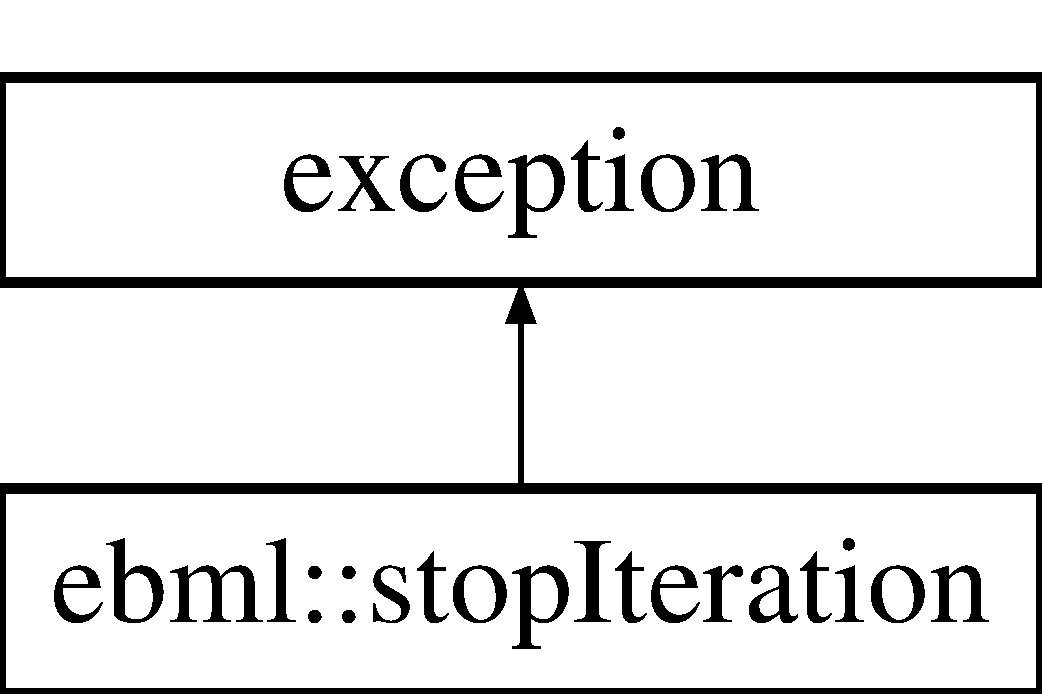
\includegraphics[height=2.000000cm]{classebml_1_1stopIteration}
\end{center}
\end{figure}


The documentation for this class was generated from the following file\+:\begin{DoxyCompactItemize}
\item 
include/libebml\+\_\+ng/\mbox{\hyperlink{exceptions_8h}{exceptions.\+h}}\end{DoxyCompactItemize}

\hypertarget{classebml_1_1unicodeDecodeError}{}\section{ebml\+:\+:unicode\+Decode\+Error Class Reference}
\label{classebml_1_1unicodeDecodeError}\index{ebml\+::unicode\+Decode\+Error@{ebml\+::unicode\+Decode\+Error}}


{\ttfamily \#include $<$exceptions.\+h$>$}

Inheritance diagram for ebml\+:\+:unicode\+Decode\+Error\+:\begin{figure}[H]
\begin{center}
\leavevmode
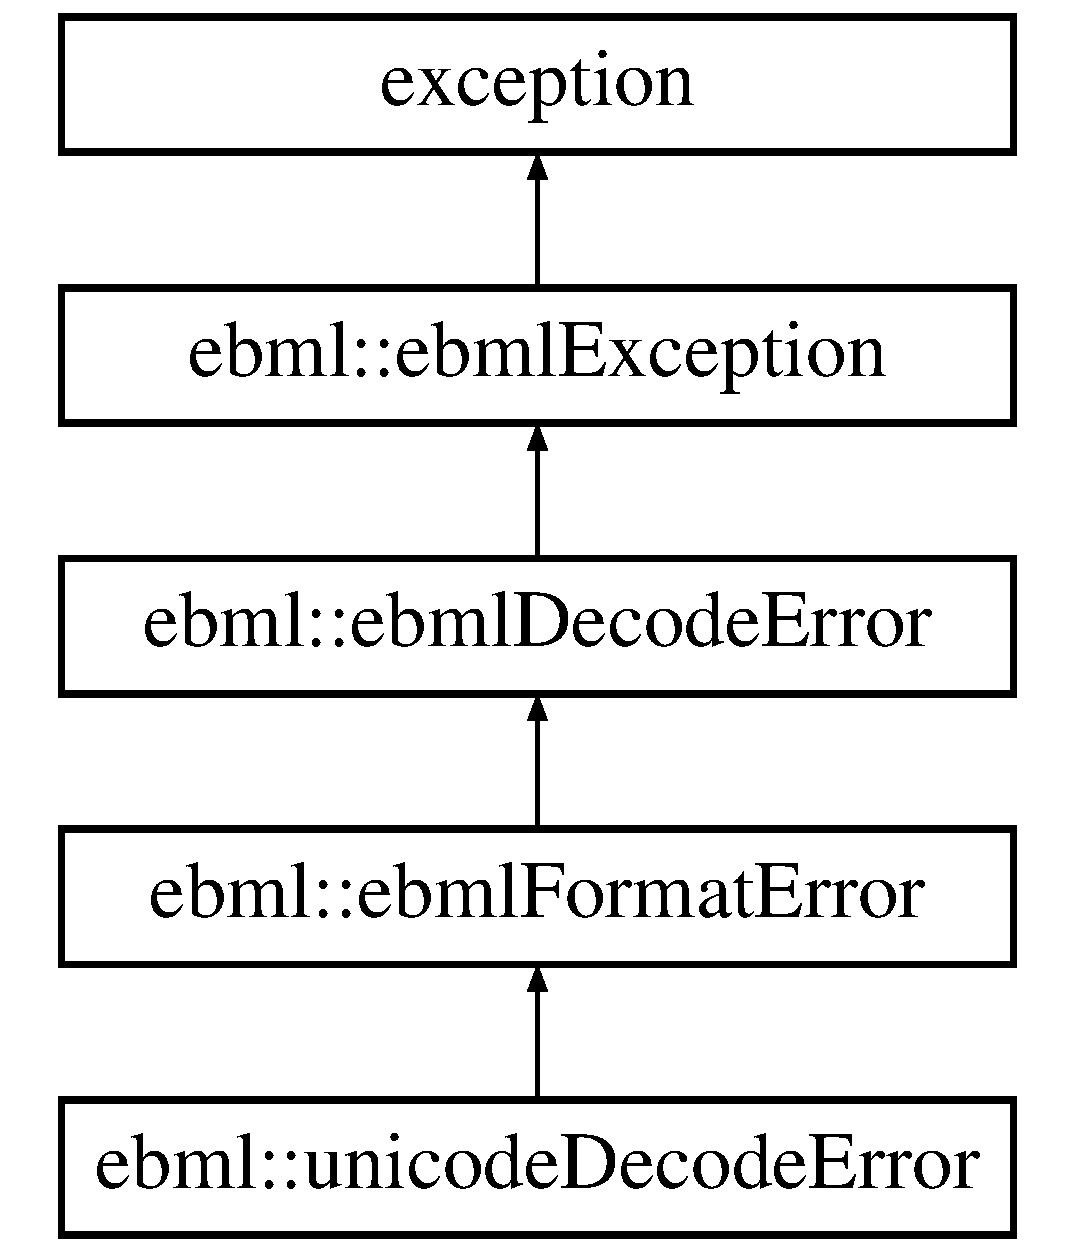
\includegraphics[height=5.000000cm]{classebml_1_1unicodeDecodeError}
\end{center}
\end{figure}
\subsection*{Public Member Functions}
\begin{DoxyCompactItemize}
\item 
\mbox{\hyperlink{classebml_1_1unicodeDecodeError_a585952785a9a0aaeb39e65e81bbabe20}{unicode\+Decode\+Error}} (const std\+::string \&message, const \mbox{\hyperlink{classebml_1_1ebmlElementClass}{ebml\+Element\+Class}} $\ast$\mbox{\hyperlink{classebml_1_1ebmlDecodeError_a3568b4ea3cd5bd16b9510abfe269920f}{cls}}=nullptr, off\+\_\+t \mbox{\hyperlink{classebml_1_1ebmlDecodeError_ad32ac9b3dd52f1c11479085d9c665e0f}{offset}}=-\/1, unsigned char \mbox{\hyperlink{classebml_1_1ebmlDecodeError_a61a4d4856f0c779a1c216e45dc5a7c1e}{head\+Size}}=0, off\+\_\+t \mbox{\hyperlink{classebml_1_1ebmlDecodeError_acb525117e0109d9640fb5e8c546e9a02}{erroroffset}}=-\/1, off\+\_\+t \mbox{\hyperlink{classebml_1_1unicodeDecodeError_aa04987ff9110293b4a5f847303559371}{end}}=-\/1, const std\+::string \&\mbox{\hyperlink{classebml_1_1unicodeDecodeError_a7a5d70226de247efb69088d0169c3dff}{object}}=\char`\"{}\char`\"{})
\end{DoxyCompactItemize}
\subsection*{Public Attributes}
\begin{DoxyCompactItemize}
\item 
std\+::string \mbox{\hyperlink{classebml_1_1unicodeDecodeError_a7a5d70226de247efb69088d0169c3dff}{object}}
\item 
off\+\_\+t \mbox{\hyperlink{classebml_1_1unicodeDecodeError_a1b1055d23aa5b2ad59b00d07ad14ab7f}{start}}
\item 
off\+\_\+t \mbox{\hyperlink{classebml_1_1unicodeDecodeError_aa04987ff9110293b4a5f847303559371}{end}}
\end{DoxyCompactItemize}


\subsection{Constructor \& Destructor Documentation}
\mbox{\Hypertarget{classebml_1_1unicodeDecodeError_a585952785a9a0aaeb39e65e81bbabe20}\label{classebml_1_1unicodeDecodeError_a585952785a9a0aaeb39e65e81bbabe20}} 
\index{ebml\+::unicode\+Decode\+Error@{ebml\+::unicode\+Decode\+Error}!unicode\+Decode\+Error@{unicode\+Decode\+Error}}
\index{unicode\+Decode\+Error@{unicode\+Decode\+Error}!ebml\+::unicode\+Decode\+Error@{ebml\+::unicode\+Decode\+Error}}
\subsubsection{\texorpdfstring{unicode\+Decode\+Error()}{unicodeDecodeError()}}
{\footnotesize\ttfamily ebml\+::unicode\+Decode\+Error\+::unicode\+Decode\+Error (\begin{DoxyParamCaption}\item[{const std\+::string \&}]{message,  }\item[{const \mbox{\hyperlink{classebml_1_1ebmlElementClass}{ebml\+Element\+Class}} $\ast$}]{cls = {\ttfamily nullptr},  }\item[{off\+\_\+t}]{offset = {\ttfamily -\/1},  }\item[{unsigned char}]{head\+Size = {\ttfamily 0},  }\item[{off\+\_\+t}]{erroroffset = {\ttfamily -\/1},  }\item[{off\+\_\+t}]{end = {\ttfamily -\/1},  }\item[{const std\+::string \&}]{object = {\ttfamily \char`\"{}\char`\"{}} }\end{DoxyParamCaption})}



\subsection{Member Data Documentation}
\mbox{\Hypertarget{classebml_1_1unicodeDecodeError_aa04987ff9110293b4a5f847303559371}\label{classebml_1_1unicodeDecodeError_aa04987ff9110293b4a5f847303559371}} 
\index{ebml\+::unicode\+Decode\+Error@{ebml\+::unicode\+Decode\+Error}!end@{end}}
\index{end@{end}!ebml\+::unicode\+Decode\+Error@{ebml\+::unicode\+Decode\+Error}}
\subsubsection{\texorpdfstring{end}{end}}
{\footnotesize\ttfamily off\+\_\+t ebml\+::unicode\+Decode\+Error\+::end}

\mbox{\Hypertarget{classebml_1_1unicodeDecodeError_a7a5d70226de247efb69088d0169c3dff}\label{classebml_1_1unicodeDecodeError_a7a5d70226de247efb69088d0169c3dff}} 
\index{ebml\+::unicode\+Decode\+Error@{ebml\+::unicode\+Decode\+Error}!object@{object}}
\index{object@{object}!ebml\+::unicode\+Decode\+Error@{ebml\+::unicode\+Decode\+Error}}
\subsubsection{\texorpdfstring{object}{object}}
{\footnotesize\ttfamily std\+::string ebml\+::unicode\+Decode\+Error\+::object}

\mbox{\Hypertarget{classebml_1_1unicodeDecodeError_a1b1055d23aa5b2ad59b00d07ad14ab7f}\label{classebml_1_1unicodeDecodeError_a1b1055d23aa5b2ad59b00d07ad14ab7f}} 
\index{ebml\+::unicode\+Decode\+Error@{ebml\+::unicode\+Decode\+Error}!start@{start}}
\index{start@{start}!ebml\+::unicode\+Decode\+Error@{ebml\+::unicode\+Decode\+Error}}
\subsubsection{\texorpdfstring{start}{start}}
{\footnotesize\ttfamily off\+\_\+t ebml\+::unicode\+Decode\+Error\+::start}



The documentation for this class was generated from the following file\+:\begin{DoxyCompactItemize}
\item 
include/libebml\+\_\+ng/\mbox{\hyperlink{exceptions_8h}{exceptions.\+h}}\end{DoxyCompactItemize}

\hypertarget{classebml_1_1unicodeEncodeError}{}\section{ebml\+:\+:unicode\+Encode\+Error Class Reference}
\label{classebml_1_1unicodeEncodeError}\index{ebml\+::unicode\+Encode\+Error@{ebml\+::unicode\+Encode\+Error}}


{\ttfamily \#include $<$exceptions.\+h$>$}

Inheritance diagram for ebml\+:\+:unicode\+Encode\+Error\+:\begin{figure}[H]
\begin{center}
\leavevmode
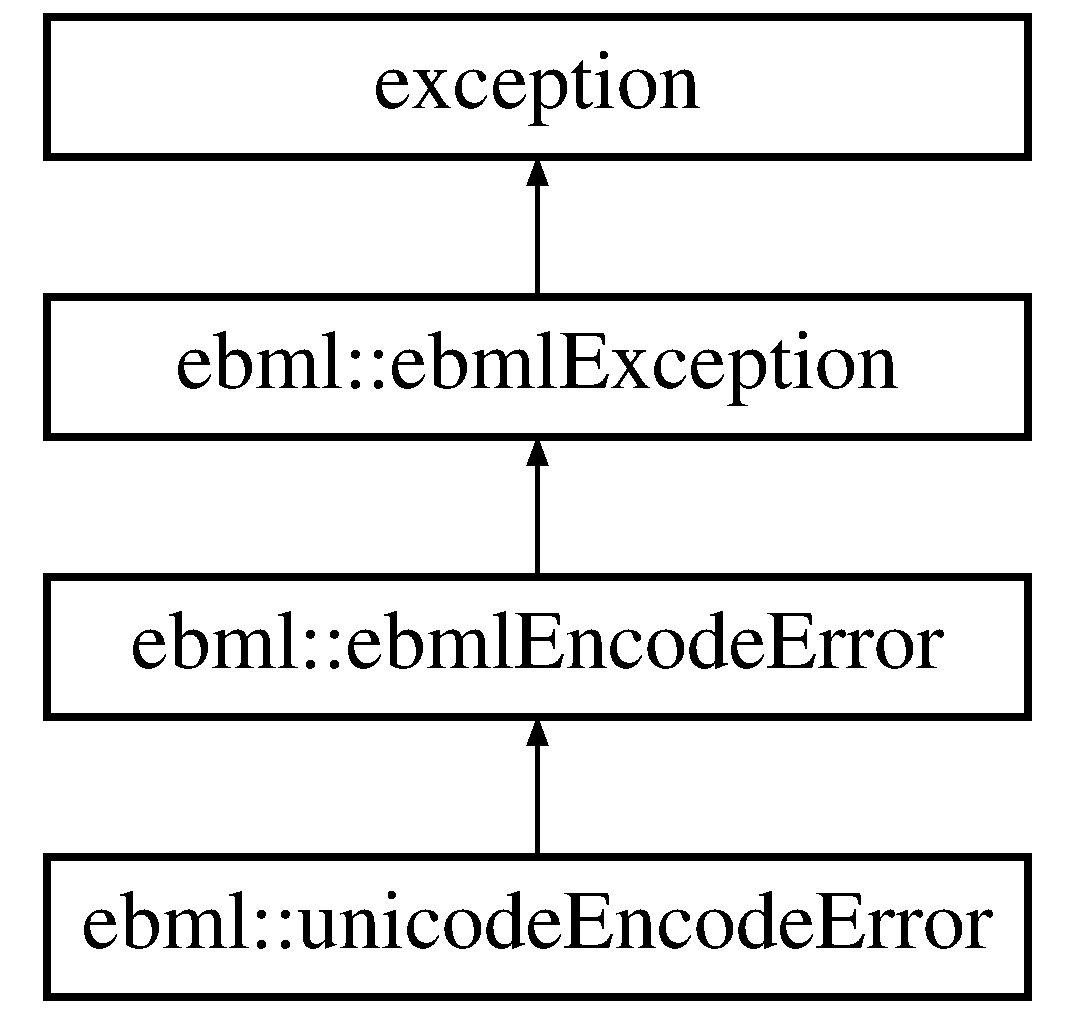
\includegraphics[height=4.000000cm]{classebml_1_1unicodeEncodeError}
\end{center}
\end{figure}
\subsection*{Public Member Functions}
\begin{DoxyCompactItemize}
\item 
\mbox{\hyperlink{classebml_1_1unicodeEncodeError_add93df3ec50e31cf17faf8170498e391}{unicode\+Encode\+Error}} (const std\+::string \&message, const std\+::wstring \&\mbox{\hyperlink{classebml_1_1unicodeEncodeError_a15a0fc868f0a45d61042220927ed17eb}{object}}=L\char`\"{}\char`\"{}, off\+\_\+t \mbox{\hyperlink{classebml_1_1unicodeEncodeError_a21775eb92e0b457166aa64892816fe68}{start}}=-\/1, off\+\_\+t \mbox{\hyperlink{classebml_1_1unicodeEncodeError_a99ec2d13b0fa0d978fe208ea45d10dba}{end}}=-\/1, const \mbox{\hyperlink{namespaceebml_a2deef4e8071531b32e3533f1bf978917}{c\+\_\+ebml\+Element\+\_\+sp}} \&\mbox{\hyperlink{classebml_1_1ebmlEncodeError_acea050cc554e717e4d9845c0cf34d473}{elem}}=nullptr)
\end{DoxyCompactItemize}
\subsection*{Public Attributes}
\begin{DoxyCompactItemize}
\item 
std\+::wstring \mbox{\hyperlink{classebml_1_1unicodeEncodeError_a15a0fc868f0a45d61042220927ed17eb}{object}}
\item 
off\+\_\+t \mbox{\hyperlink{classebml_1_1unicodeEncodeError_a21775eb92e0b457166aa64892816fe68}{start}}
\item 
off\+\_\+t \mbox{\hyperlink{classebml_1_1unicodeEncodeError_a99ec2d13b0fa0d978fe208ea45d10dba}{end}}
\end{DoxyCompactItemize}


\subsection{Constructor \& Destructor Documentation}
\mbox{\Hypertarget{classebml_1_1unicodeEncodeError_add93df3ec50e31cf17faf8170498e391}\label{classebml_1_1unicodeEncodeError_add93df3ec50e31cf17faf8170498e391}} 
\index{ebml\+::unicode\+Encode\+Error@{ebml\+::unicode\+Encode\+Error}!unicode\+Encode\+Error@{unicode\+Encode\+Error}}
\index{unicode\+Encode\+Error@{unicode\+Encode\+Error}!ebml\+::unicode\+Encode\+Error@{ebml\+::unicode\+Encode\+Error}}
\subsubsection{\texorpdfstring{unicode\+Encode\+Error()}{unicodeEncodeError()}}
{\footnotesize\ttfamily ebml\+::unicode\+Encode\+Error\+::unicode\+Encode\+Error (\begin{DoxyParamCaption}\item[{const std\+::string \&}]{message,  }\item[{const std\+::wstring \&}]{object = {\ttfamily L\char`\"{}\char`\"{}},  }\item[{off\+\_\+t}]{start = {\ttfamily -\/1},  }\item[{off\+\_\+t}]{end = {\ttfamily -\/1},  }\item[{const \mbox{\hyperlink{namespaceebml_a2deef4e8071531b32e3533f1bf978917}{c\+\_\+ebml\+Element\+\_\+sp}} \&}]{elem = {\ttfamily nullptr} }\end{DoxyParamCaption})}



\subsection{Member Data Documentation}
\mbox{\Hypertarget{classebml_1_1unicodeEncodeError_a99ec2d13b0fa0d978fe208ea45d10dba}\label{classebml_1_1unicodeEncodeError_a99ec2d13b0fa0d978fe208ea45d10dba}} 
\index{ebml\+::unicode\+Encode\+Error@{ebml\+::unicode\+Encode\+Error}!end@{end}}
\index{end@{end}!ebml\+::unicode\+Encode\+Error@{ebml\+::unicode\+Encode\+Error}}
\subsubsection{\texorpdfstring{end}{end}}
{\footnotesize\ttfamily off\+\_\+t ebml\+::unicode\+Encode\+Error\+::end}

\mbox{\Hypertarget{classebml_1_1unicodeEncodeError_a15a0fc868f0a45d61042220927ed17eb}\label{classebml_1_1unicodeEncodeError_a15a0fc868f0a45d61042220927ed17eb}} 
\index{ebml\+::unicode\+Encode\+Error@{ebml\+::unicode\+Encode\+Error}!object@{object}}
\index{object@{object}!ebml\+::unicode\+Encode\+Error@{ebml\+::unicode\+Encode\+Error}}
\subsubsection{\texorpdfstring{object}{object}}
{\footnotesize\ttfamily std\+::wstring ebml\+::unicode\+Encode\+Error\+::object}

\mbox{\Hypertarget{classebml_1_1unicodeEncodeError_a21775eb92e0b457166aa64892816fe68}\label{classebml_1_1unicodeEncodeError_a21775eb92e0b457166aa64892816fe68}} 
\index{ebml\+::unicode\+Encode\+Error@{ebml\+::unicode\+Encode\+Error}!start@{start}}
\index{start@{start}!ebml\+::unicode\+Encode\+Error@{ebml\+::unicode\+Encode\+Error}}
\subsubsection{\texorpdfstring{start}{start}}
{\footnotesize\ttfamily off\+\_\+t ebml\+::unicode\+Encode\+Error\+::start}



The documentation for this class was generated from the following file\+:\begin{DoxyCompactItemize}
\item 
include/libebml\+\_\+ng/\mbox{\hyperlink{exceptions_8h}{exceptions.\+h}}\end{DoxyCompactItemize}

\chapter{File Documentation}
\hypertarget{libebml__ng_8h}{}\section{include/libebml\+\_\+ng.h File Reference}
\label{libebml__ng_8h}\index{include/libebml\+\_\+ng.\+h@{include/libebml\+\_\+ng.\+h}}
{\ttfamily \#include \char`\"{}libebml\+\_\+ng/masterelement/map.\+h\char`\"{}}\newline
\subsection*{Namespaces}
\begin{DoxyCompactItemize}
\item 
 \mbox{\hyperlink{namespaceebml}{ebml}}
\end{DoxyCompactItemize}

\hypertarget{basictypes_8h}{}\section{include/libebml\+\_\+ng/basictypes.h File Reference}
\label{basictypes_8h}\index{include/libebml\+\_\+ng/basictypes.\+h@{include/libebml\+\_\+ng/basictypes.\+h}}
{\ttfamily \#include \char`\"{}libebml\+\_\+ng/template.\+h\char`\"{}}\newline
{\ttfamily \#include \char`\"{}libebml\+\_\+ng/struct/datetime.\+h\char`\"{}}\newline
\subsection*{Namespaces}
\begin{DoxyCompactItemize}
\item 
 \mbox{\hyperlink{namespaceebml}{ebml}}
\end{DoxyCompactItemize}
\subsection*{Macros}
\begin{DoxyCompactItemize}
\item 
\#define \mbox{\hyperlink{basictypes_8h_a04d01fea6c31ddb4b4b90243898815f2}{D\+E\+C\+L\+\_\+\+E\+B\+M\+L\+\_\+\+C\+LS}}(T)
\item 
\#define \mbox{\hyperlink{basictypes_8h_a5ed837e62ab25ec444f4a263a8a84d3a}{D\+E\+C\+L\+\_\+\+E\+B\+M\+L\+\_\+\+A\+L\+I\+AS}}(T,  alias)
\end{DoxyCompactItemize}
\subsection*{Typedefs}
\begin{DoxyCompactItemize}
\item 
typedef \+::\mbox{\hyperlink{classebml_1_1ebmlDataElementClass}{ebml\+::ebml\+Data\+Element\+Class}}$<$ unsigned long long $>$ \mbox{\hyperlink{namespaceebml_a506b246c5594e5d0322c3c05e9820fd2}{ebml\+::ebml\+Unsigned\+Integer\+Class}}
\item 
typedef \+::\mbox{\hyperlink{classebml_1_1ebmlDataElement}{ebml\+::ebml\+Data\+Element}}$<$ unsigned long long $>$ \mbox{\hyperlink{namespaceebml_a094d15ef60da5dd0e74a4e379ac3e547}{ebml\+::ebml\+Unsigned\+Integer}}
\item 
typedef \+::\mbox{\hyperlink{classebml_1_1ebmlDataElementClass}{ebml\+::ebml\+Data\+Element\+Class}}$<$ long long $>$ \mbox{\hyperlink{namespaceebml_a344220b1a75e640887ea0d280f2349af}{ebml\+::ebml\+Signed\+Integer\+Class}}
\item 
typedef \+::\mbox{\hyperlink{classebml_1_1ebmlDataElement}{ebml\+::ebml\+Data\+Element}}$<$ long long $>$ \mbox{\hyperlink{namespaceebml_a5429f4885c9e4e9eeda85b245ea6166a}{ebml\+::ebml\+Signed\+Integer}}
\item 
typedef \+::\mbox{\hyperlink{classebml_1_1ebmlDataElementClass}{ebml\+::ebml\+Data\+Element\+Class}}$<$ double $>$ \mbox{\hyperlink{namespaceebml_a2e365f10ba5435bdd5c1fd909a601f31}{ebml\+::ebml\+Float\+Class}}
\item 
typedef \+::\mbox{\hyperlink{classebml_1_1ebmlDataElement}{ebml\+::ebml\+Data\+Element}}$<$ double $>$ \mbox{\hyperlink{namespaceebml_af998fa3b620e1bb7363e1426c9910b9c}{ebml\+::ebml\+Float}}
\item 
typedef \+::\mbox{\hyperlink{classebml_1_1ebmlDataElementClass}{ebml\+::ebml\+Data\+Element\+Class}}$<$ std\+::string $>$ \mbox{\hyperlink{namespaceebml_a4fe139b904ac34f0e3036c9451b4b18b}{ebml\+::ebml\+Binary\+Class}}
\item 
typedef \+::\mbox{\hyperlink{classebml_1_1ebmlDataElement}{ebml\+::ebml\+Data\+Element}}$<$ std\+::string $>$ \mbox{\hyperlink{namespaceebml_a9b2775bff9ce97bc09b955ca1de557ae}{ebml\+::ebml\+Binary}}
\item 
typedef \+::\mbox{\hyperlink{classebml_1_1ebmlDataElementClass}{ebml\+::ebml\+Data\+Element\+Class}}$<$ std\+::wstring $>$ \mbox{\hyperlink{namespaceebml_acdb74e752b77d5b4a4c445684db86832}{ebml\+::ebml\+Unicode\+Class}}
\item 
typedef \+::\mbox{\hyperlink{classebml_1_1ebmlDataElement}{ebml\+::ebml\+Data\+Element}}$<$ std\+::wstring $>$ \mbox{\hyperlink{namespaceebml_abd9662588801df32dd1d2853a9f2f9b1}{ebml\+::ebml\+Unicode}}
\item 
typedef \+::\mbox{\hyperlink{classebml_1_1ebmlDataElementClass}{ebml\+::ebml\+Data\+Element\+Class}}$<$ timepoint\+\_\+t $>$ \mbox{\hyperlink{namespaceebml_afea0376d38786592ad3e71d619256ab5}{ebml\+::ebml\+Date\+Time\+Class}}
\item 
typedef \+::\mbox{\hyperlink{classebml_1_1ebmlDataElement}{ebml\+::ebml\+Data\+Element}}$<$ timepoint\+\_\+t $>$ \mbox{\hyperlink{namespaceebml_a544c5c28e36511ffd20b5907e551754f}{ebml\+::ebml\+Date\+Time}}
\end{DoxyCompactItemize}
\subsection*{Functions}
\begin{DoxyCompactItemize}
\item 
template std\+::string \& \mbox{\hyperlink{basictypes_8h_a788046c0c8a46dc9a4a09058207a0c7d}{ebml\+::data$<$ std\+::string $>$}} (const ebml\+Element\+\_\+sp \&)
\item 
template const std\+::string \& \mbox{\hyperlink{basictypes_8h_af6a36b3fcf97793a79307054680f8f99}{ebml\+::data$<$ std\+::string $>$}} (const c\+\_\+ebml\+Element\+\_\+sp \&)
\item 
template std\+::wstring \& \mbox{\hyperlink{basictypes_8h_a73482a0a9b59a94c3609ba1088763841}{ebml\+::data$<$ std\+::wstring $>$}} (const ebml\+Element\+\_\+sp \&)
\item 
template const std\+::wstring \& \mbox{\hyperlink{basictypes_8h_abfb55840338be40beeaa3955bc138c5f}{ebml\+::data$<$ std\+::wstring $>$}} (const c\+\_\+ebml\+Element\+\_\+sp \&)
\item 
template \mbox{\hyperlink{namespaceebml_a7e667ec3fe8b51fb5b8f9690734d8638}{ebml\+::timepoint\+\_\+t}} \& \mbox{\hyperlink{basictypes_8h_aa49e89a4a0b27b990b15e79b0f11f88b}{ebml\+::data$<$ ebml\+::timepoint\+\_\+t $>$}} (const ebml\+Element\+\_\+sp \&)
\item 
template const \mbox{\hyperlink{namespaceebml_a7e667ec3fe8b51fb5b8f9690734d8638}{ebml\+::timepoint\+\_\+t}} \& \mbox{\hyperlink{basictypes_8h_aa8f72fbfba4027da262a9912c73a301a}{ebml\+::data$<$ ebml\+::timepoint\+\_\+t $>$}} (const c\+\_\+ebml\+Element\+\_\+sp \&)
\end{DoxyCompactItemize}


\subsection{Macro Definition Documentation}
\mbox{\Hypertarget{basictypes_8h_a5ed837e62ab25ec444f4a263a8a84d3a}\label{basictypes_8h_a5ed837e62ab25ec444f4a263a8a84d3a}} 
\index{basictypes.\+h@{basictypes.\+h}!D\+E\+C\+L\+\_\+\+E\+B\+M\+L\+\_\+\+A\+L\+I\+AS@{D\+E\+C\+L\+\_\+\+E\+B\+M\+L\+\_\+\+A\+L\+I\+AS}}
\index{D\+E\+C\+L\+\_\+\+E\+B\+M\+L\+\_\+\+A\+L\+I\+AS@{D\+E\+C\+L\+\_\+\+E\+B\+M\+L\+\_\+\+A\+L\+I\+AS}!basictypes.\+h@{basictypes.\+h}}
\subsubsection{\texorpdfstring{D\+E\+C\+L\+\_\+\+E\+B\+M\+L\+\_\+\+A\+L\+I\+AS}{DECL\_EBML\_ALIAS}}
{\footnotesize\ttfamily \#define D\+E\+C\+L\+\_\+\+E\+B\+M\+L\+\_\+\+A\+L\+I\+AS(\begin{DoxyParamCaption}\item[{}]{T,  }\item[{}]{alias }\end{DoxyParamCaption})}

{\bfseries Value\+:}
\begin{DoxyCode}
typedef ::ebml::ebmlDataElementClass<T> alias##Class; \(\backslash\)
    typedef ::ebml::ebmlDataElement<T> alias;
\end{DoxyCode}
\mbox{\Hypertarget{basictypes_8h_a04d01fea6c31ddb4b4b90243898815f2}\label{basictypes_8h_a04d01fea6c31ddb4b4b90243898815f2}} 
\index{basictypes.\+h@{basictypes.\+h}!D\+E\+C\+L\+\_\+\+E\+B\+M\+L\+\_\+\+C\+LS@{D\+E\+C\+L\+\_\+\+E\+B\+M\+L\+\_\+\+C\+LS}}
\index{D\+E\+C\+L\+\_\+\+E\+B\+M\+L\+\_\+\+C\+LS@{D\+E\+C\+L\+\_\+\+E\+B\+M\+L\+\_\+\+C\+LS}!basictypes.\+h@{basictypes.\+h}}
\subsubsection{\texorpdfstring{D\+E\+C\+L\+\_\+\+E\+B\+M\+L\+\_\+\+C\+LS}{DECL\_EBML\_CLS}}
{\footnotesize\ttfamily \#define D\+E\+C\+L\+\_\+\+E\+B\+M\+L\+\_\+\+C\+LS(\begin{DoxyParamCaption}\item[{}]{T }\end{DoxyParamCaption})}

{\bfseries Value\+:}
\begin{DoxyCode}
\textcolor{keyword}{extern} \textcolor{keyword}{template} \textcolor{keyword}{class }\mbox{\hyperlink{classebml_1_1ebmlDataElementClass}{ebml::ebmlDataElementClass<T>}}; \(\backslash\)
    extern \textcolor{keyword}{template} \textcolor{keyword}{class }\mbox{\hyperlink{classebml_1_1ebmlDataElement}{ebml::ebmlDataElement<T>}}; \(\backslash\)
    extern \textcolor{keyword}{template} T& ebml::data<T>(\textcolor{keyword}{const} \mbox{\hyperlink{namespaceebml_adad533b7705a16bb360fe56380c5e7be}{ebmlElement\_sp}}&); \(\backslash\)
    extern \textcolor{keyword}{template} \textcolor{keyword}{const} T& ebml::data<T>(\textcolor{keyword}{const} \mbox{\hyperlink{namespaceebml_a2deef4e8071531b32e3533f1bf978917}{c\_ebmlElement\_sp}}&);
\end{DoxyCode}


\subsection{Function Documentation}
\mbox{\Hypertarget{basictypes_8h_aa49e89a4a0b27b990b15e79b0f11f88b}\label{basictypes_8h_aa49e89a4a0b27b990b15e79b0f11f88b}} 
\index{basictypes.\+h@{basictypes.\+h}!ebml\+::data$<$ ebml\+::timepoint\+\_\+t $>$@{ebml\+::data$<$ ebml\+::timepoint\+\_\+t $>$}}
\index{ebml\+::data$<$ ebml\+::timepoint\+\_\+t $>$@{ebml\+::data$<$ ebml\+::timepoint\+\_\+t $>$}!basictypes.\+h@{basictypes.\+h}}
\subsubsection{\texorpdfstring{ebml\+::data$<$ ebml\+::timepoint\+\_\+t $>$()}{ebml::data< ebml::timepoint\_t >()}\hspace{0.1cm}{\footnotesize\ttfamily [1/2]}}
{\footnotesize\ttfamily template \mbox{\hyperlink{namespaceebml_a7e667ec3fe8b51fb5b8f9690734d8638}{ebml\+::timepoint\+\_\+t}}\& \mbox{\hyperlink{namespaceebml_a6365629b3110a3c5d0cde94d08aac26c}{ebml\+::data}}$<$ \mbox{\hyperlink{namespaceebml_a7e667ec3fe8b51fb5b8f9690734d8638}{ebml\+::timepoint\+\_\+t}} $>$ (\begin{DoxyParamCaption}\item[{const ebml\+Element\+\_\+sp \&}]{ }\end{DoxyParamCaption})}

\mbox{\Hypertarget{basictypes_8h_aa8f72fbfba4027da262a9912c73a301a}\label{basictypes_8h_aa8f72fbfba4027da262a9912c73a301a}} 
\index{basictypes.\+h@{basictypes.\+h}!ebml\+::data$<$ ebml\+::timepoint\+\_\+t $>$@{ebml\+::data$<$ ebml\+::timepoint\+\_\+t $>$}}
\index{ebml\+::data$<$ ebml\+::timepoint\+\_\+t $>$@{ebml\+::data$<$ ebml\+::timepoint\+\_\+t $>$}!basictypes.\+h@{basictypes.\+h}}
\subsubsection{\texorpdfstring{ebml\+::data$<$ ebml\+::timepoint\+\_\+t $>$()}{ebml::data< ebml::timepoint\_t >()}\hspace{0.1cm}{\footnotesize\ttfamily [2/2]}}
{\footnotesize\ttfamily template const \mbox{\hyperlink{namespaceebml_a7e667ec3fe8b51fb5b8f9690734d8638}{ebml\+::timepoint\+\_\+t}}\& \mbox{\hyperlink{namespaceebml_a6365629b3110a3c5d0cde94d08aac26c}{ebml\+::data}}$<$ \mbox{\hyperlink{namespaceebml_a7e667ec3fe8b51fb5b8f9690734d8638}{ebml\+::timepoint\+\_\+t}} $>$ (\begin{DoxyParamCaption}\item[{const c\+\_\+ebml\+Element\+\_\+sp \&}]{ }\end{DoxyParamCaption})}

\mbox{\Hypertarget{basictypes_8h_af6a36b3fcf97793a79307054680f8f99}\label{basictypes_8h_af6a36b3fcf97793a79307054680f8f99}} 
\index{basictypes.\+h@{basictypes.\+h}!ebml\+::data$<$ std\+::string $>$@{ebml\+::data$<$ std\+::string $>$}}
\index{ebml\+::data$<$ std\+::string $>$@{ebml\+::data$<$ std\+::string $>$}!basictypes.\+h@{basictypes.\+h}}
\subsubsection{\texorpdfstring{ebml\+::data$<$ std\+::string $>$()}{ebml::data< std::string >()}\hspace{0.1cm}{\footnotesize\ttfamily [1/2]}}
{\footnotesize\ttfamily template const std\+::string\& \mbox{\hyperlink{namespaceebml_a6365629b3110a3c5d0cde94d08aac26c}{ebml\+::data}}$<$ std\+::string $>$ (\begin{DoxyParamCaption}\item[{const c\+\_\+ebml\+Element\+\_\+sp \&}]{ }\end{DoxyParamCaption})}

\mbox{\Hypertarget{basictypes_8h_a788046c0c8a46dc9a4a09058207a0c7d}\label{basictypes_8h_a788046c0c8a46dc9a4a09058207a0c7d}} 
\index{basictypes.\+h@{basictypes.\+h}!ebml\+::data$<$ std\+::string $>$@{ebml\+::data$<$ std\+::string $>$}}
\index{ebml\+::data$<$ std\+::string $>$@{ebml\+::data$<$ std\+::string $>$}!basictypes.\+h@{basictypes.\+h}}
\subsubsection{\texorpdfstring{ebml\+::data$<$ std\+::string $>$()}{ebml::data< std::string >()}\hspace{0.1cm}{\footnotesize\ttfamily [2/2]}}
{\footnotesize\ttfamily template std\+::string\& \mbox{\hyperlink{namespaceebml_a6365629b3110a3c5d0cde94d08aac26c}{ebml\+::data}}$<$ std\+::string $>$ (\begin{DoxyParamCaption}\item[{const ebml\+Element\+\_\+sp \&}]{ }\end{DoxyParamCaption})}

\mbox{\Hypertarget{basictypes_8h_a73482a0a9b59a94c3609ba1088763841}\label{basictypes_8h_a73482a0a9b59a94c3609ba1088763841}} 
\index{basictypes.\+h@{basictypes.\+h}!ebml\+::data$<$ std\+::wstring $>$@{ebml\+::data$<$ std\+::wstring $>$}}
\index{ebml\+::data$<$ std\+::wstring $>$@{ebml\+::data$<$ std\+::wstring $>$}!basictypes.\+h@{basictypes.\+h}}
\subsubsection{\texorpdfstring{ebml\+::data$<$ std\+::wstring $>$()}{ebml::data< std::wstring >()}\hspace{0.1cm}{\footnotesize\ttfamily [1/2]}}
{\footnotesize\ttfamily template std\+::wstring\& \mbox{\hyperlink{namespaceebml_a6365629b3110a3c5d0cde94d08aac26c}{ebml\+::data}}$<$ std\+::wstring $>$ (\begin{DoxyParamCaption}\item[{const ebml\+Element\+\_\+sp \&}]{ }\end{DoxyParamCaption})}

\mbox{\Hypertarget{basictypes_8h_abfb55840338be40beeaa3955bc138c5f}\label{basictypes_8h_abfb55840338be40beeaa3955bc138c5f}} 
\index{basictypes.\+h@{basictypes.\+h}!ebml\+::data$<$ std\+::wstring $>$@{ebml\+::data$<$ std\+::wstring $>$}}
\index{ebml\+::data$<$ std\+::wstring $>$@{ebml\+::data$<$ std\+::wstring $>$}!basictypes.\+h@{basictypes.\+h}}
\subsubsection{\texorpdfstring{ebml\+::data$<$ std\+::wstring $>$()}{ebml::data< std::wstring >()}\hspace{0.1cm}{\footnotesize\ttfamily [2/2]}}
{\footnotesize\ttfamily template const std\+::wstring\& \mbox{\hyperlink{namespaceebml_a6365629b3110a3c5d0cde94d08aac26c}{ebml\+::data}}$<$ std\+::wstring $>$ (\begin{DoxyParamCaption}\item[{const c\+\_\+ebml\+Element\+\_\+sp \&}]{ }\end{DoxyParamCaption})}


\input{dataelement_8h}
\input{document_8h}
\hypertarget{ebmlID__t_8h}{}\section{include/libebml\+\_\+ng/ebml\+I\+D\+\_\+t.h File Reference}
\label{ebmlID__t_8h}\index{include/libebml\+\_\+ng/ebml\+I\+D\+\_\+t.\+h@{include/libebml\+\_\+ng/ebml\+I\+D\+\_\+t.\+h}}
\subsection*{Namespaces}
\begin{DoxyCompactItemize}
\item 
 \mbox{\hyperlink{namespaceebml}{ebml}}
\end{DoxyCompactItemize}
\subsection*{Typedefs}
\begin{DoxyCompactItemize}
\item 
typedef unsigned long long \mbox{\hyperlink{namespaceebml_a86c5f604ddf12a74aa9812e997a58691}{ebml\+::ebml\+I\+D\+\_\+t}}
\item 
typedef unsigned char \mbox{\hyperlink{namespaceebml_a2ccdfb60b23efb51fe07f9d066e23604}{ebml\+::vint\+Width\+\_\+t}}
\end{DoxyCompactItemize}

\input{element_8h}
\input{elementcls_8h}
\hypertarget{exceptions_8h}{}\section{include/libebml\+\_\+ng/exceptions.h File Reference}
\label{exceptions_8h}\index{include/libebml\+\_\+ng/exceptions.\+h@{include/libebml\+\_\+ng/exceptions.\+h}}
{\ttfamily \#include $<$string$>$}\newline
{\ttfamily \#include \char`\"{}base.\+h\char`\"{}}\newline
\subsection*{Classes}
\begin{DoxyCompactItemize}
\item 
class \mbox{\hyperlink{classebml_1_1stopIteration}{ebml\+::stop\+Iteration}}
\item 
class \mbox{\hyperlink{classebml_1_1ebmlException}{ebml\+::ebml\+Exception}}
\item 
class \mbox{\hyperlink{classebml_1_1ebmlNotImplementedError}{ebml\+::ebml\+Not\+Implemented\+Error}}
\item 
class \mbox{\hyperlink{classebml_1_1ebmlEncodeError}{ebml\+::ebml\+Encode\+Error}}
\item 
class \mbox{\hyperlink{classebml_1_1ebmlDecodeError}{ebml\+::ebml\+Decode\+Error}}
\item 
class \mbox{\hyperlink{classebml_1_1ebmlInvalidVint}{ebml\+::ebml\+Invalid\+Vint}}
\item 
class \mbox{\hyperlink{classebml_1_1ebmlNoMatch}{ebml\+::ebml\+No\+Match}}
\item 
class \mbox{\hyperlink{classebml_1_1ebmlNoChildMatch}{ebml\+::ebml\+No\+Child\+Match}}
\item 
class \mbox{\hyperlink{classebml_1_1ebmlUnexpectedEndOfData}{ebml\+::ebml\+Unexpected\+End\+Of\+Data}}
\item 
class \mbox{\hyperlink{classebml_1_1ebmlDataContinues}{ebml\+::ebml\+Data\+Continues}}
\item 
class \mbox{\hyperlink{classebml_1_1ebmlFormatError}{ebml\+::ebml\+Format\+Error}}
\item 
class \mbox{\hyperlink{classebml_1_1unicodeDecodeError}{ebml\+::unicode\+Decode\+Error}}
\item 
class \mbox{\hyperlink{classebml_1_1unicodeEncodeError}{ebml\+::unicode\+Encode\+Error}}
\end{DoxyCompactItemize}
\subsection*{Namespaces}
\begin{DoxyCompactItemize}
\item 
 \mbox{\hyperlink{namespaceebml}{ebml}}
\end{DoxyCompactItemize}
\subsection*{Macros}
\begin{DoxyCompactItemize}
\item 
\#define \mbox{\hyperlink{exceptions_8h_a01ee6217c68541f80344fef107abc5fe}{D\+E\+C\+O\+D\+E\+\_\+\+E\+R\+R\+\_\+\+S\+I\+G\+\_\+\+D\+E\+CL}}~const std\+::string\& message, const ebml\+Element\+Class$\ast$ cls=nullptr, off\+\_\+t offset=-\/1, unsigned char head\+Size=0, off\+\_\+t erroroffset=-\/1
\item 
\#define \mbox{\hyperlink{exceptions_8h_a89caf3bc22758eb2ef85c9699a5cbaaa}{D\+E\+C\+O\+D\+E\+\_\+\+E\+R\+R\+\_\+\+S\+IG}}~const std\+::string\& message, const ebml\+Element\+Class$\ast$ cls, off\+\_\+t offset, unsigned char head\+Size, off\+\_\+t erroroffset
\item 
\#define \mbox{\hyperlink{exceptions_8h_a208012d6b09554374a4dc0254a7749af}{D\+E\+C\+O\+D\+E\+\_\+\+E\+R\+R\+\_\+\+A\+R\+GS}}~message, cls, offset, head\+Size, erroroffset
\item 
\#define \mbox{\hyperlink{exceptions_8h_a7786f4d58118605f83b1850a18053091}{D\+E\+C\+O\+D\+E\+\_\+\+E\+R\+R\+\_\+\+D\+E\+F\+A\+U\+LT}}~nullptr, 0, 0
\end{DoxyCompactItemize}
\subsection*{Functions}
\begin{DoxyCompactItemize}
\item 
std\+::string \mbox{\hyperlink{namespaceebml_a41bf8a299c4418f406beff89817b0690}{ebml\+::make\+\_\+exc\+\_\+msg}} (const char $\ast$msg, unsigned int lineno, const char $\ast$file)
\end{DoxyCompactItemize}


\subsection{Macro Definition Documentation}
\mbox{\Hypertarget{exceptions_8h_a208012d6b09554374a4dc0254a7749af}\label{exceptions_8h_a208012d6b09554374a4dc0254a7749af}} 
\index{exceptions.\+h@{exceptions.\+h}!D\+E\+C\+O\+D\+E\+\_\+\+E\+R\+R\+\_\+\+A\+R\+GS@{D\+E\+C\+O\+D\+E\+\_\+\+E\+R\+R\+\_\+\+A\+R\+GS}}
\index{D\+E\+C\+O\+D\+E\+\_\+\+E\+R\+R\+\_\+\+A\+R\+GS@{D\+E\+C\+O\+D\+E\+\_\+\+E\+R\+R\+\_\+\+A\+R\+GS}!exceptions.\+h@{exceptions.\+h}}
\subsubsection{\texorpdfstring{D\+E\+C\+O\+D\+E\+\_\+\+E\+R\+R\+\_\+\+A\+R\+GS}{DECODE\_ERR\_ARGS}}
{\footnotesize\ttfamily \#define D\+E\+C\+O\+D\+E\+\_\+\+E\+R\+R\+\_\+\+A\+R\+GS~message, cls, offset, head\+Size, erroroffset}

\mbox{\Hypertarget{exceptions_8h_a7786f4d58118605f83b1850a18053091}\label{exceptions_8h_a7786f4d58118605f83b1850a18053091}} 
\index{exceptions.\+h@{exceptions.\+h}!D\+E\+C\+O\+D\+E\+\_\+\+E\+R\+R\+\_\+\+D\+E\+F\+A\+U\+LT@{D\+E\+C\+O\+D\+E\+\_\+\+E\+R\+R\+\_\+\+D\+E\+F\+A\+U\+LT}}
\index{D\+E\+C\+O\+D\+E\+\_\+\+E\+R\+R\+\_\+\+D\+E\+F\+A\+U\+LT@{D\+E\+C\+O\+D\+E\+\_\+\+E\+R\+R\+\_\+\+D\+E\+F\+A\+U\+LT}!exceptions.\+h@{exceptions.\+h}}
\subsubsection{\texorpdfstring{D\+E\+C\+O\+D\+E\+\_\+\+E\+R\+R\+\_\+\+D\+E\+F\+A\+U\+LT}{DECODE\_ERR\_DEFAULT}}
{\footnotesize\ttfamily \#define D\+E\+C\+O\+D\+E\+\_\+\+E\+R\+R\+\_\+\+D\+E\+F\+A\+U\+LT~nullptr, 0, 0}

\mbox{\Hypertarget{exceptions_8h_a89caf3bc22758eb2ef85c9699a5cbaaa}\label{exceptions_8h_a89caf3bc22758eb2ef85c9699a5cbaaa}} 
\index{exceptions.\+h@{exceptions.\+h}!D\+E\+C\+O\+D\+E\+\_\+\+E\+R\+R\+\_\+\+S\+IG@{D\+E\+C\+O\+D\+E\+\_\+\+E\+R\+R\+\_\+\+S\+IG}}
\index{D\+E\+C\+O\+D\+E\+\_\+\+E\+R\+R\+\_\+\+S\+IG@{D\+E\+C\+O\+D\+E\+\_\+\+E\+R\+R\+\_\+\+S\+IG}!exceptions.\+h@{exceptions.\+h}}
\subsubsection{\texorpdfstring{D\+E\+C\+O\+D\+E\+\_\+\+E\+R\+R\+\_\+\+S\+IG}{DECODE\_ERR\_SIG}}
{\footnotesize\ttfamily \#define D\+E\+C\+O\+D\+E\+\_\+\+E\+R\+R\+\_\+\+S\+IG~const std\+::string\& message, const ebml\+Element\+Class$\ast$ cls, off\+\_\+t offset, unsigned char head\+Size, off\+\_\+t erroroffset}

\mbox{\Hypertarget{exceptions_8h_a01ee6217c68541f80344fef107abc5fe}\label{exceptions_8h_a01ee6217c68541f80344fef107abc5fe}} 
\index{exceptions.\+h@{exceptions.\+h}!D\+E\+C\+O\+D\+E\+\_\+\+E\+R\+R\+\_\+\+S\+I\+G\+\_\+\+D\+E\+CL@{D\+E\+C\+O\+D\+E\+\_\+\+E\+R\+R\+\_\+\+S\+I\+G\+\_\+\+D\+E\+CL}}
\index{D\+E\+C\+O\+D\+E\+\_\+\+E\+R\+R\+\_\+\+S\+I\+G\+\_\+\+D\+E\+CL@{D\+E\+C\+O\+D\+E\+\_\+\+E\+R\+R\+\_\+\+S\+I\+G\+\_\+\+D\+E\+CL}!exceptions.\+h@{exceptions.\+h}}
\subsubsection{\texorpdfstring{D\+E\+C\+O\+D\+E\+\_\+\+E\+R\+R\+\_\+\+S\+I\+G\+\_\+\+D\+E\+CL}{DECODE\_ERR\_SIG\_DECL}}
{\footnotesize\ttfamily \#define D\+E\+C\+O\+D\+E\+\_\+\+E\+R\+R\+\_\+\+S\+I\+G\+\_\+\+D\+E\+CL~const std\+::string\& message, const ebml\+Element\+Class$\ast$ cls=nullptr, off\+\_\+t offset=-\/1, unsigned char head\+Size=0, off\+\_\+t erroroffset=-\/1}


\input{forwards_8h}
\hypertarget{head_8h}{}\section{include/libebml\+\_\+ng/head.h File Reference}
\label{head_8h}\index{include/libebml\+\_\+ng/head.\+h@{include/libebml\+\_\+ng/head.\+h}}
{\ttfamily \#include \char`\"{}basictypes.\+h\char`\"{}}\newline
{\ttfamily \#include \char`\"{}masterelement/multislot.\+h\char`\"{}}\newline
\subsection*{Namespaces}
\begin{DoxyCompactItemize}
\item 
 \mbox{\hyperlink{namespaceebml}{ebml}}
\end{DoxyCompactItemize}
\subsection*{Variables}
\begin{DoxyCompactItemize}
\item 
ebml\+Unsigned\+Integer\+Class \mbox{\hyperlink{namespaceebml_ab043f0427daa3a4eb36615002a603c2f}{ebml\+::\+E\+B\+M\+L\+Version}}
\item 
ebml\+Unsigned\+Integer\+Class \mbox{\hyperlink{namespaceebml_ae2a831962d9fe406ade51a61f4d7f44f}{ebml\+::\+E\+B\+M\+L\+Read\+Version}}
\item 
ebml\+Unsigned\+Integer\+Class \mbox{\hyperlink{namespaceebml_aa5391f5da29eee93d9bbb4faef121430}{ebml\+::\+E\+B\+M\+L\+Max\+I\+D\+Length}}
\item 
ebml\+Unsigned\+Integer\+Class \mbox{\hyperlink{namespaceebml_a2f4a3ca0aa5867e5024d72b48328ee65}{ebml\+::\+E\+B\+M\+L\+Max\+Size\+Length}}
\item 
ebml\+Binary\+Class \mbox{\hyperlink{namespaceebml_ad196ce572692673a986be2bdabf9907b}{ebml\+::\+Doc\+Type}}
\item 
ebml\+Unsigned\+Integer\+Class \mbox{\hyperlink{namespaceebml_a4bfea9b659c99c0f0d0dc51026f480ca}{ebml\+::\+Doc\+Type\+Version}}
\item 
ebml\+Unsigned\+Integer\+Class \mbox{\hyperlink{namespaceebml_acd5324e76213e2721983c93bd909eeff}{ebml\+::\+Doc\+Type\+Read\+Version}}
\item 
ebml\+Multi\+Slot\+Class \mbox{\hyperlink{namespaceebml_a969dbd2316937386e704f1aae53ed8b9}{ebml\+::\+E\+B\+M\+L\+Head}}
\end{DoxyCompactItemize}

\hypertarget{io_8h}{}\section{include/libebml\+\_\+ng/io.h File Reference}
\label{io_8h}\index{include/libebml\+\_\+ng/io.\+h@{include/libebml\+\_\+ng/io.\+h}}
{\ttfamily \#include $<$mutex$>$}\newline
{\ttfamily \#include $<$memory$>$}\newline
{\ttfamily \#include $<$iostream$>$}\newline
{\ttfamily \#include \char`\"{}ptrs.\+h\char`\"{}}\newline
\subsection*{Classes}
\begin{DoxyCompactItemize}
\item 
class \mbox{\hyperlink{classebml_1_1ioBase}{ebml\+::io\+Base}}
\item 
class \mbox{\hyperlink{classebml_1_1io}{ebml\+::io$<$ T $>$}}
\end{DoxyCompactItemize}
\subsection*{Namespaces}
\begin{DoxyCompactItemize}
\item 
 \mbox{\hyperlink{namespaceebml}{ebml}}
\end{DoxyCompactItemize}

\hypertarget{parsing_2io_8h}{}\section{include/libebml\+\_\+ng/parsing/io.h File Reference}
\label{parsing_2io_8h}\index{include/libebml\+\_\+ng/parsing/io.\+h@{include/libebml\+\_\+ng/parsing/io.\+h}}
{\ttfamily \#include $<$memory$>$}\newline
{\ttfamily \#include \char`\"{}libebml\+\_\+ng/ebml\+I\+D\+\_\+t.\+h\char`\"{}}\newline
{\ttfamily \#include \char`\"{}libebml\+\_\+ng/io.\+h\char`\"{}}\newline
\subsection*{Classes}
\begin{DoxyCompactItemize}
\item 
class \mbox{\hyperlink{classebml_1_1parseFile}{ebml\+::parse\+File}}
\item 
class \mbox{\hyperlink{classebml_1_1parseFile_1_1iterator}{ebml\+::parse\+File\+::iterator}}
\end{DoxyCompactItemize}
\subsection*{Namespaces}
\begin{DoxyCompactItemize}
\item 
 \mbox{\hyperlink{namespaceebml}{ebml}}
\end{DoxyCompactItemize}

\hypertarget{__fd_8h}{}\section{include/libebml\+\_\+ng/io/\+\_\+fd.h File Reference}
\label{__fd_8h}\index{include/libebml\+\_\+ng/io/\+\_\+fd.\+h@{include/libebml\+\_\+ng/io/\+\_\+fd.\+h}}
{\ttfamily \#include \char`\"{}libebml\+\_\+ng/io.\+h\char`\"{}}\newline
\subsection*{Namespaces}
\begin{DoxyCompactItemize}
\item 
 \mbox{\hyperlink{namespaceebml}{ebml}}
\end{DoxyCompactItemize}

\hypertarget{__stdio_8h}{}\section{include/libebml\+\_\+ng/io/\+\_\+stdio.h File Reference}
\label{__stdio_8h}\index{include/libebml\+\_\+ng/io/\+\_\+stdio.\+h@{include/libebml\+\_\+ng/io/\+\_\+stdio.\+h}}
{\ttfamily \#include \char`\"{}libebml\+\_\+ng/io.\+h\char`\"{}}\newline
{\ttfamily \#include $<$stdio.\+h$>$}\newline
\subsection*{Namespaces}
\begin{DoxyCompactItemize}
\item 
 \mbox{\hyperlink{namespaceebml}{ebml}}
\end{DoxyCompactItemize}

\hypertarget{fd_8h}{}\section{include/libebml\+\_\+ng/io/fd.h File Reference}
\label{fd_8h}\index{include/libebml\+\_\+ng/io/fd.\+h@{include/libebml\+\_\+ng/io/fd.\+h}}
{\ttfamily \#include \char`\"{}libebml\+\_\+ng/io.\+h\char`\"{}}\newline
\subsection*{Namespaces}
\begin{DoxyCompactItemize}
\item 
 \mbox{\hyperlink{namespaceebml}{ebml}}
\end{DoxyCompactItemize}

\hypertarget{stdio_8h}{}\section{include/libebml\+\_\+ng/io/stdio.h File Reference}
\label{stdio_8h}\index{include/libebml\+\_\+ng/io/stdio.\+h@{include/libebml\+\_\+ng/io/stdio.\+h}}
{\ttfamily \#include \char`\"{}libebml\+\_\+ng/io.\+h\char`\"{}}\newline
{\ttfamily \#include $<$stdio.\+h$>$}\newline
\subsection*{Namespaces}
\begin{DoxyCompactItemize}
\item 
 \mbox{\hyperlink{namespaceebml}{ebml}}
\end{DoxyCompactItemize}

\hypertarget{base_8h}{}\section{include/libebml\+\_\+ng/base.h File Reference}
\label{base_8h}\index{include/libebml\+\_\+ng/base.\+h@{include/libebml\+\_\+ng/base.\+h}}
{\ttfamily \#include \char`\"{}stdio.\+h\char`\"{}}\newline
{\ttfamily \#include $<$iostream$>$}\newline
{\ttfamily \#include $<$exception$>$}\newline
{\ttfamily \#include $<$memory$>$}\newline
{\ttfamily \#include $<$mutex$>$}\newline
{\ttfamily \#include $<$iomanip$>$}\newline
{\ttfamily \#include $<$sstream$>$}\newline
{\ttfamily \#include \char`\"{}parsing/string.\+h\char`\"{}}\newline
{\ttfamily \#include \char`\"{}parsing/io.\+h\char`\"{}}\newline
{\ttfamily \#include \char`\"{}vint.\+h\char`\"{}}\newline
\subsection*{Classes}
\begin{DoxyCompactItemize}
\item 
class \mbox{\hyperlink{classebml_1_1ebmlElementClass}{ebml\+::ebml\+Element\+Class}}
\item 
class \mbox{\hyperlink{classebml_1_1ebmlElement}{ebml\+::ebml\+Element}}
\item 
class \mbox{\hyperlink{classebml_1_1ebmlVoidClass}{ebml\+::ebml\+Void\+Class}}
\item 
class \mbox{\hyperlink{classebml_1_1ebmlVoid}{ebml\+::ebml\+Void}}
\item 
class \mbox{\hyperlink{classebml_1_1ebmlDocument}{ebml\+::ebml\+Document}}
\end{DoxyCompactItemize}
\subsection*{Namespaces}
\begin{DoxyCompactItemize}
\item 
 \mbox{\hyperlink{namespaceebml}{ebml}}
\end{DoxyCompactItemize}
\subsection*{Typedefs}
\begin{DoxyCompactItemize}
\item 
typedef std\+::shared\+\_\+ptr$<$ ebml\+Element $>$ \mbox{\hyperlink{namespaceebml_adad533b7705a16bb360fe56380c5e7be}{ebml\+::ebml\+Element\+\_\+sp}}
\item 
typedef std\+::shared\+\_\+ptr$<$ const ebml\+Element $>$ \mbox{\hyperlink{namespaceebml_a2deef4e8071531b32e3533f1bf978917}{ebml\+::c\+\_\+ebml\+Element\+\_\+sp}}
\item 
typedef std\+::weak\+\_\+ptr$<$ ebml\+Element $>$ \mbox{\hyperlink{namespaceebml_a495fb58b42b0050d887415351af02935}{ebml\+::ebml\+Element\+\_\+wp}}
\item 
typedef std\+::weak\+\_\+ptr$<$ const ebml\+Element $>$ \mbox{\hyperlink{namespaceebml_abc218c2fc1444b2fd8a8a5fae67e0151}{ebml\+::c\+\_\+ebml\+Element\+\_\+wp}}
\item 
typedef std\+::shared\+\_\+ptr$<$ ebml\+Document $>$ \mbox{\hyperlink{namespaceebml_a66018942b568da5041136a945148b450}{ebml\+::ebml\+Document\+\_\+sp}}
\item 
typedef std\+::weak\+\_\+ptr$<$ ebml\+Document $>$ \mbox{\hyperlink{namespaceebml_acfead4f724a6f8d55c730c6fbd362cea}{ebml\+::ebml\+Document\+\_\+wp}}
\end{DoxyCompactItemize}
\subsection*{Variables}
\begin{DoxyCompactItemize}
\item 
ebml\+Void\+Class \mbox{\hyperlink{namespaceebml_afbfd509d1cb71e416a07253746e886e9}{ebml\+::\+Void}}
\end{DoxyCompactItemize}

\hypertarget{lazyload_8h}{}\section{include/libebml\+\_\+ng/masterelement/lazyload.h File Reference}
\label{lazyload_8h}\index{include/libebml\+\_\+ng/masterelement/lazyload.\+h@{include/libebml\+\_\+ng/masterelement/lazyload.\+h}}
{\ttfamily \#include \char`\"{}libebml\+\_\+ng/masterelement.\+h\char`\"{}}\newline
{\ttfamily \#include $<$unordered\+\_\+map$>$}\newline
{\ttfamily \#include $<$unordered\+\_\+set$>$}\newline
{\ttfamily \#include $<$mutex$>$}\newline
\subsection*{Classes}
\begin{DoxyCompactItemize}
\item 
class \mbox{\hyperlink{classebml_1_1ebmlLazyLoadMasterElement}{ebml\+::ebml\+Lazy\+Load\+Master\+Element}}
\item 
class \mbox{\hyperlink{classebml_1_1ebmlLazyLoadMasterElement_1_1localLock}{ebml\+::ebml\+Lazy\+Load\+Master\+Element\+::local\+Lock}}
\end{DoxyCompactItemize}
\subsection*{Namespaces}
\begin{DoxyCompactItemize}
\item 
 \mbox{\hyperlink{namespaceebml}{ebml}}
\end{DoxyCompactItemize}

\hypertarget{list_8h}{}\section{include/libebml\+\_\+ng/masterelement/list.h File Reference}
\label{list_8h}\index{include/libebml\+\_\+ng/masterelement/list.\+h@{include/libebml\+\_\+ng/masterelement/list.\+h}}
{\ttfamily \#include \char`\"{}libebml\+\_\+ng/base.\+h\char`\"{}}\newline
{\ttfamily \#include \char`\"{}libebml\+\_\+ng/masterelement/base.\+h\char`\"{}}\newline
{\ttfamily \#include $<$unordered\+\_\+map$>$}\newline
{\ttfamily \#include $<$vector$>$}\newline
\subsection*{Classes}
\begin{DoxyCompactItemize}
\item 
class \mbox{\hyperlink{classebml_1_1ebmlListClass}{ebml\+::ebml\+List\+Class}}
\item 
class \mbox{\hyperlink{classebml_1_1ebmlList}{ebml\+::ebml\+List}}
\item 
class \mbox{\hyperlink{classebml_1_1ebmlList_1_1__iterator}{ebml\+::ebml\+List\+::\+\_\+iterator}}
\item 
class \mbox{\hyperlink{classebml_1_1ebmlList_1_1__const__iterator}{ebml\+::ebml\+List\+::\+\_\+const\+\_\+iterator}}
\end{DoxyCompactItemize}
\subsection*{Namespaces}
\begin{DoxyCompactItemize}
\item 
 \mbox{\hyperlink{namespaceebml}{ebml}}
\end{DoxyCompactItemize}

\hypertarget{map_8h}{}\section{include/libebml\+\_\+ng/masterelement/map.h File Reference}
\label{map_8h}\index{include/libebml\+\_\+ng/masterelement/map.\+h@{include/libebml\+\_\+ng/masterelement/map.\+h}}
{\ttfamily \#include $<$unordered\+\_\+map$>$}\newline
{\ttfamily \#include $<$vector$>$}\newline
{\ttfamily \#include $<$exception$>$}\newline
{\ttfamily \#include \char`\"{}base.\+h\char`\"{}}\newline
{\ttfamily \#include \char`\"{}../dataelement.\+h\char`\"{}}\newline
{\ttfamily \#include \char`\"{}../element.\+h\char`\"{}}\newline
\subsection*{Classes}
\begin{DoxyCompactItemize}
\item 
class \mbox{\hyperlink{classebml_1_1ebmlPair}{ebml\+::ebml\+Pair$<$ T $>$}}
\item 
class \mbox{\hyperlink{classebml_1_1ebmlPairClass}{ebml\+::ebml\+Pair\+Class$<$ T $>$}}
\item 
class \mbox{\hyperlink{classebml_1_1ebmlMap}{ebml\+::ebml\+Map$<$ K, H, E, A $>$}}
\item 
class \mbox{\hyperlink{classebml_1_1ebmlPair}{ebml\+::ebml\+Pair$<$ T $>$}}
\item 
class \mbox{\hyperlink{classebml_1_1ebmlPair_1_1__iterator}{ebml\+::ebml\+Pair$<$ T $>$\+::\+\_\+iterator}}
\item 
class \mbox{\hyperlink{classebml_1_1ebmlPair_1_1__const__iterator}{ebml\+::ebml\+Pair$<$ T $>$\+::\+\_\+const\+\_\+iterator}}
\item 
class \mbox{\hyperlink{classebml_1_1ebmlMapClass}{ebml\+::ebml\+Map\+Class$<$ K, H, E, A $>$}}
\item 
class \mbox{\hyperlink{classebml_1_1ebmlMap}{ebml\+::ebml\+Map$<$ K, H, E, A $>$}}
\item 
class \mbox{\hyperlink{classebml_1_1ebmlMap_1_1__iterator}{ebml\+::ebml\+Map$<$ K, H, E, A $>$\+::\+\_\+iterator}}
\item 
class \mbox{\hyperlink{classebml_1_1ebmlMap_1_1__const__iterator}{ebml\+::ebml\+Map$<$ K, H, E, A $>$\+::\+\_\+const\+\_\+iterator}}
\end{DoxyCompactItemize}
\subsection*{Namespaces}
\begin{DoxyCompactItemize}
\item 
 \mbox{\hyperlink{namespaceebml}{ebml}}
\end{DoxyCompactItemize}
\subsection*{Macros}
\begin{DoxyCompactItemize}
\item 
\#define \mbox{\hyperlink{map_8h_a10d1bc3373c0ed867047e97ff67b817b}{E\+X\+T\+E\+R\+N\+\_\+\+M\+A\+P\+\_\+\+T\+Y\+PE}}(K\+E\+Y\+T\+Y\+PE)
\item 
\#define \mbox{\hyperlink{map_8h_a10270459a5e10e99993436737aefa4df}{I\+N\+S\+T\+\_\+\+M\+A\+P\+\_\+\+T\+Y\+PE}}(K\+E\+Y\+T\+Y\+PE)
\item 
\#define \mbox{\hyperlink{map_8h_a3988a61dbdd2e59792a4c6b33b25f257}{E\+X\+T\+E\+R\+N\+\_\+\+M\+A\+P\+\_\+\+T\+Y\+P\+E\+\_\+\+E\+XT}}(K\+E\+Y\+T\+Y\+PE, ...)
\item 
\#define \mbox{\hyperlink{map_8h_a29b085432761b0895688d72d0a08f381}{I\+N\+S\+T\+\_\+\+M\+A\+P\+\_\+\+T\+Y\+P\+E\+\_\+\+E\+XT}}(K\+E\+Y\+T\+Y\+PE, ...)
\end{DoxyCompactItemize}
\subsection*{Typedefs}
\begin{DoxyCompactItemize}
\item 
{\footnotesize template$<$typename T $>$ }\\using \mbox{\hyperlink{namespaceebml_a15439f6031c0f4ced33b9ab5e28af120}{ebml\+::ebml\+Pair\+\_\+sp}} = std\+::shared\+\_\+ptr$<$ ebml\+Pair$<$ T $>$ $>$
\item 
{\footnotesize template$<$typename T $>$ }\\using \mbox{\hyperlink{namespaceebml_a9c804317d5b51ef8844bdffe5e8cb4b3}{ebml\+::c\+\_\+ebml\+Pair\+\_\+sp}} = std\+::shared\+\_\+ptr$<$ const ebml\+Pair$<$ T $>$ $>$
\end{DoxyCompactItemize}


\subsection{Macro Definition Documentation}
\mbox{\Hypertarget{map_8h_a10d1bc3373c0ed867047e97ff67b817b}\label{map_8h_a10d1bc3373c0ed867047e97ff67b817b}} 
\index{map.\+h@{map.\+h}!E\+X\+T\+E\+R\+N\+\_\+\+M\+A\+P\+\_\+\+T\+Y\+PE@{E\+X\+T\+E\+R\+N\+\_\+\+M\+A\+P\+\_\+\+T\+Y\+PE}}
\index{E\+X\+T\+E\+R\+N\+\_\+\+M\+A\+P\+\_\+\+T\+Y\+PE@{E\+X\+T\+E\+R\+N\+\_\+\+M\+A\+P\+\_\+\+T\+Y\+PE}!map.\+h@{map.\+h}}
\subsubsection{\texorpdfstring{E\+X\+T\+E\+R\+N\+\_\+\+M\+A\+P\+\_\+\+T\+Y\+PE}{EXTERN\_MAP\_TYPE}}
{\footnotesize\ttfamily \#define E\+X\+T\+E\+R\+N\+\_\+\+M\+A\+P\+\_\+\+T\+Y\+PE(\begin{DoxyParamCaption}\item[{}]{K\+E\+Y\+T\+Y\+PE }\end{DoxyParamCaption})}

{\bfseries Value\+:}
\begin{DoxyCode}
\textcolor{keyword}{extern} \textcolor{keyword}{template} \textcolor{keyword}{class }\mbox{\hyperlink{classebml_1_1ebmlPairClass}{ebml::ebmlPairClass<const KEYTYPE>}}; \(\backslash\)
    extern \textcolor{keyword}{template} \textcolor{keyword}{class }\mbox{\hyperlink{classebml_1_1ebmlPair}{ebml::ebmlPair<const KEYTYPE>}}; \(\backslash\)
    EXTERN\_AS\_MEMBERS(\mbox{\hyperlink{classebml_1_1ebmlPairClass}{ebml::ebmlPairClass<const KEYTYPE>}}, 
      \mbox{\hyperlink{classebml_1_1ebmlPair}{ebml::ebmlPair<const KEYTYPE>}}) \(\backslash\)
    extern \textcolor{keyword}{template} \textcolor{keyword}{class }\mbox{\hyperlink{classebml_1_1ebmlMapClass}{ebml::ebmlMapClass<KEYTYPE>}}; \(\backslash\)
    extern \textcolor{keyword}{template} \textcolor{keyword}{class }\mbox{\hyperlink{classebml_1_1ebmlMap}{ebml::ebmlMap<KEYTYPE>}}; \(\backslash\)
    EXTERN\_AS\_MEMBERS(\mbox{\hyperlink{classebml_1_1ebmlMapClass}{ebml::ebmlMapClass<KEYTYPE>}}, 
      \mbox{\hyperlink{classebml_1_1ebmlMap}{ebml::ebmlMap<KEYTYPE>}})
\end{DoxyCode}
\mbox{\Hypertarget{map_8h_a3988a61dbdd2e59792a4c6b33b25f257}\label{map_8h_a3988a61dbdd2e59792a4c6b33b25f257}} 
\index{map.\+h@{map.\+h}!E\+X\+T\+E\+R\+N\+\_\+\+M\+A\+P\+\_\+\+T\+Y\+P\+E\+\_\+\+E\+XT@{E\+X\+T\+E\+R\+N\+\_\+\+M\+A\+P\+\_\+\+T\+Y\+P\+E\+\_\+\+E\+XT}}
\index{E\+X\+T\+E\+R\+N\+\_\+\+M\+A\+P\+\_\+\+T\+Y\+P\+E\+\_\+\+E\+XT@{E\+X\+T\+E\+R\+N\+\_\+\+M\+A\+P\+\_\+\+T\+Y\+P\+E\+\_\+\+E\+XT}!map.\+h@{map.\+h}}
\subsubsection{\texorpdfstring{E\+X\+T\+E\+R\+N\+\_\+\+M\+A\+P\+\_\+\+T\+Y\+P\+E\+\_\+\+E\+XT}{EXTERN\_MAP\_TYPE\_EXT}}
{\footnotesize\ttfamily \#define E\+X\+T\+E\+R\+N\+\_\+\+M\+A\+P\+\_\+\+T\+Y\+P\+E\+\_\+\+E\+XT(\begin{DoxyParamCaption}\item[{}]{K\+E\+Y\+T\+Y\+PE,  }\item[{}]{... }\end{DoxyParamCaption})}

{\bfseries Value\+:}
\begin{DoxyCode}
\textcolor{keyword}{extern} \textcolor{keyword}{template} \textcolor{keyword}{class }\mbox{\hyperlink{classebml_1_1ebmlPairClass}{ebml::ebmlPairClass<const KEYTYPE>}}; \(\backslash\)
    extern \textcolor{keyword}{template} \textcolor{keyword}{class }\mbox{\hyperlink{classebml_1_1ebmlPair}{ebml::ebmlPair<const KEYTYPE>}}; \(\backslash\)
    EXTERN\_AS\_MEMBERS(\mbox{\hyperlink{classebml_1_1ebmlPairClass}{ebml::ebmlPairClass<const KEYTYPE>}}, 
      \mbox{\hyperlink{classebml_1_1ebmlPair}{ebml::ebmlPair<const KEYTYPE>}}) \(\backslash\)
    extern \textcolor{keyword}{template} \textcolor{keyword}{class }\mbox{\hyperlink{classebml_1_1ebmlMapClass}{ebml::ebmlMapClass<KEYTYPE, ##\_\_VA\_ARGS\_\_>}}
      ; \(\backslash\)
    extern \textcolor{keyword}{template} \textcolor{keyword}{class }\mbox{\hyperlink{classebml_1_1ebmlMap}{ebml::ebmlMap<KEYTYPE, ##\_\_VA\_ARGS\_\_>}}; \(\backslash\)
    EXTERN\_AS\_MEMBERS(\mbox{\hyperlink{classebml_1_1ebmlMapClass}{ebml::ebmlMapClass<KEYTYPE, ##\_\_VA\_ARGS\_\_>}},
       \mbox{\hyperlink{classebml_1_1ebmlMap}{ebml::ebmlMap<KEYTYPE, ##\_\_VA\_ARGS\_\_>}})
\end{DoxyCode}
\mbox{\Hypertarget{map_8h_a10270459a5e10e99993436737aefa4df}\label{map_8h_a10270459a5e10e99993436737aefa4df}} 
\index{map.\+h@{map.\+h}!I\+N\+S\+T\+\_\+\+M\+A\+P\+\_\+\+T\+Y\+PE@{I\+N\+S\+T\+\_\+\+M\+A\+P\+\_\+\+T\+Y\+PE}}
\index{I\+N\+S\+T\+\_\+\+M\+A\+P\+\_\+\+T\+Y\+PE@{I\+N\+S\+T\+\_\+\+M\+A\+P\+\_\+\+T\+Y\+PE}!map.\+h@{map.\+h}}
\subsubsection{\texorpdfstring{I\+N\+S\+T\+\_\+\+M\+A\+P\+\_\+\+T\+Y\+PE}{INST\_MAP\_TYPE}}
{\footnotesize\ttfamily \#define I\+N\+S\+T\+\_\+\+M\+A\+P\+\_\+\+T\+Y\+PE(\begin{DoxyParamCaption}\item[{}]{K\+E\+Y\+T\+Y\+PE }\end{DoxyParamCaption})}

{\bfseries Value\+:}
\begin{DoxyCode}
\textcolor{keyword}{template} \textcolor{keyword}{class }\mbox{\hyperlink{classebml_1_1ebmlPairClass}{ebml::ebmlPairClass<const KEYTYPE>}}; \(\backslash\)
    template \textcolor{keyword}{class }\mbox{\hyperlink{classebml_1_1ebmlPair}{ebml::ebmlPair<const KEYTYPE>}}; \(\backslash\)
    INST\_AS\_MEMBERS(\mbox{\hyperlink{classebml_1_1ebmlPairClass}{ebml::ebmlPairClass<const KEYTYPE>}}, 
      \mbox{\hyperlink{classebml_1_1ebmlPair}{ebml::ebmlPair<const KEYTYPE>}}) \(\backslash\)
    template \textcolor{keyword}{class }\mbox{\hyperlink{classebml_1_1ebmlMapClass}{ebml::ebmlMapClass<KEYTYPE>}}; \(\backslash\)
    template \textcolor{keyword}{class }\mbox{\hyperlink{classebml_1_1ebmlMap}{ebml::ebmlMap<KEYTYPE>}}; \(\backslash\)
    INST\_AS\_MEMBERS(\mbox{\hyperlink{classebml_1_1ebmlMapClass}{ebml::ebmlMapClass<KEYTYPE>}}, 
      \mbox{\hyperlink{classebml_1_1ebmlMap}{ebml::ebmlMap<KEYTYPE>}})
\end{DoxyCode}
\mbox{\Hypertarget{map_8h_a29b085432761b0895688d72d0a08f381}\label{map_8h_a29b085432761b0895688d72d0a08f381}} 
\index{map.\+h@{map.\+h}!I\+N\+S\+T\+\_\+\+M\+A\+P\+\_\+\+T\+Y\+P\+E\+\_\+\+E\+XT@{I\+N\+S\+T\+\_\+\+M\+A\+P\+\_\+\+T\+Y\+P\+E\+\_\+\+E\+XT}}
\index{I\+N\+S\+T\+\_\+\+M\+A\+P\+\_\+\+T\+Y\+P\+E\+\_\+\+E\+XT@{I\+N\+S\+T\+\_\+\+M\+A\+P\+\_\+\+T\+Y\+P\+E\+\_\+\+E\+XT}!map.\+h@{map.\+h}}
\subsubsection{\texorpdfstring{I\+N\+S\+T\+\_\+\+M\+A\+P\+\_\+\+T\+Y\+P\+E\+\_\+\+E\+XT}{INST\_MAP\_TYPE\_EXT}}
{\footnotesize\ttfamily \#define I\+N\+S\+T\+\_\+\+M\+A\+P\+\_\+\+T\+Y\+P\+E\+\_\+\+E\+XT(\begin{DoxyParamCaption}\item[{}]{K\+E\+Y\+T\+Y\+PE,  }\item[{}]{... }\end{DoxyParamCaption})}

{\bfseries Value\+:}
\begin{DoxyCode}
\textcolor{keyword}{template} \textcolor{keyword}{class }\mbox{\hyperlink{classebml_1_1ebmlPairClass}{ebml::ebmlPairClass<const KEYTYPE>}}; \(\backslash\)
    template \textcolor{keyword}{class }\mbox{\hyperlink{classebml_1_1ebmlPair}{ebml::ebmlPair<const KEYTYPE>}}; \(\backslash\)
    INST\_AS\_MEMBERS(\mbox{\hyperlink{classebml_1_1ebmlPairClass}{ebml::ebmlPairClass<const KEYTYPE>}}, 
      \mbox{\hyperlink{classebml_1_1ebmlPair}{ebml::ebmlPair<const KEYTYPE>}}) \(\backslash\)
    template \textcolor{keyword}{class }\mbox{\hyperlink{classebml_1_1ebmlMapClass}{ebml::ebmlMapClass<KEYTYPE, ##\_\_VA\_ARGS\_\_>}}; \(\backslash\)
    template \textcolor{keyword}{class }\mbox{\hyperlink{classebml_1_1ebmlMap}{ebml::ebmlMap<KEYTYPE, ##\_\_VA\_ARGS\_\_>}}; \(\backslash\)
    INST\_AS\_MEMBERS(\mbox{\hyperlink{classebml_1_1ebmlMapClass}{ebml::ebmlMapClass<KEYTYPE, ##\_\_VA\_ARGS\_\_>}}, 
      \mbox{\hyperlink{classebml_1_1ebmlMap}{ebml::ebmlMap<KEYTYPE, ##\_\_VA\_ARGS\_\_>}})
\end{DoxyCode}

\hypertarget{multislot_8h}{}\section{include/libebml\+\_\+ng/masterelement/multislot.h File Reference}
\label{multislot_8h}\index{include/libebml\+\_\+ng/masterelement/multislot.\+h@{include/libebml\+\_\+ng/masterelement/multislot.\+h}}
{\ttfamily \#include \char`\"{}libebml\+\_\+ng/base.\+h\char`\"{}}\newline
{\ttfamily \#include \char`\"{}libebml\+\_\+ng/masterelement/base.\+h\char`\"{}}\newline
{\ttfamily \#include $<$unordered\+\_\+map$>$}\newline
{\ttfamily \#include $<$vector$>$}\newline
{\ttfamily \#include $<$variant$>$}\newline
{\ttfamily \#include $<$ext/new\+\_\+allocator.\+h$>$}\newline
\subsection*{Classes}
\begin{DoxyCompactItemize}
\item 
class \mbox{\hyperlink{classebml_1_1slotSpec__t}{ebml\+::slot\+Spec\+\_\+t}}
\item 
class \mbox{\hyperlink{classebml_1_1ebmlMultiSlotClass}{ebml\+::ebml\+Multi\+Slot\+Class}}
\item 
class \mbox{\hyperlink{classebml_1_1slotArg__t}{ebml\+::slot\+Arg\+\_\+t}}
\item 
class \mbox{\hyperlink{classebml_1_1const__slot__t}{ebml\+::const\+\_\+slot\+\_\+t}}
\item 
class \mbox{\hyperlink{classebml_1_1const__slot__t_1_1iterator}{ebml\+::const\+\_\+slot\+\_\+t\+::iterator}}
\item 
class \mbox{\hyperlink{classebml_1_1slot__t}{ebml\+::slot\+\_\+t}}
\item 
class \mbox{\hyperlink{classebml_1_1slot__t_1_1iterator}{ebml\+::slot\+\_\+t\+::iterator}}
\item 
class \mbox{\hyperlink{classebml_1_1ebmlMultiSlot}{ebml\+::ebml\+Multi\+Slot}}
\item 
class \mbox{\hyperlink{classebml_1_1ebmlMultiSlot_1_1__iterator}{ebml\+::ebml\+Multi\+Slot\+::\+\_\+iterator}}
\item 
class \mbox{\hyperlink{classebml_1_1ebmlMultiSlot_1_1__const__iterator}{ebml\+::ebml\+Multi\+Slot\+::\+\_\+const\+\_\+iterator}}
\end{DoxyCompactItemize}
\subsection*{Namespaces}
\begin{DoxyCompactItemize}
\item 
 \mbox{\hyperlink{namespaceebml}{ebml}}
\end{DoxyCompactItemize}
\subsection*{Typedefs}
\begin{DoxyCompactItemize}
\item 
typedef std\+::vector$<$ slot\+Spec\+\_\+t $>$ \mbox{\hyperlink{namespaceebml_abdc1248164e4e424423defac9fff7d4d}{ebml\+::slot\+Spec\+\_\+l}}
\item 
typedef std\+::list$<$ slot\+Arg\+\_\+t $>$ \mbox{\hyperlink{namespaceebml_ae432575dfbb3e141ce897442794f0ca5}{ebml\+::slot\+Arg\+\_\+l}}
\item 
typedef std\+::unordered\+\_\+map$<$ std\+::string, slot\+Arg\+\_\+t $>$ \mbox{\hyperlink{namespaceebml_a4317d4c495715eced3ed448c2d05caeb}{ebml\+::slot\+Arg\+\_\+d}}
\item 
typedef std\+::shared\+\_\+ptr$<$ ebml\+Multi\+Slot $>$ \mbox{\hyperlink{namespaceebml_a1e633eb51fcbe25caf953fd159171543}{ebml\+::ebml\+Multi\+Slot\+\_\+sp}}
\item 
typedef std\+::shared\+\_\+ptr$<$ const ebml\+Multi\+Slot $>$ \mbox{\hyperlink{namespaceebml_a2b7466e45489d2a5dbfa29b411eb4ed0}{ebml\+::c\+\_\+ebml\+Multi\+Slot\+\_\+sp}}
\end{DoxyCompactItemize}
\subsection*{Functions}
\begin{DoxyCompactItemize}
\item 
{\footnotesize template$<$typename T $>$ }\\T \mbox{\hyperlink{namespaceebml_a766ff55857f1018516a926913abc8a83}{ebml\+::data}} (const const\+\_\+slot\+\_\+t \&slot)
\item 
{\footnotesize template$<$typename T $>$ }\\T \& \mbox{\hyperlink{namespaceebml_ad2539ebb0462e9038828f80590adf688}{ebml\+::data}} (slot\+\_\+t \&slot)
\end{DoxyCompactItemize}

\hypertarget{io__noseek_8h}{}\section{include/libebml\+\_\+ng/parsing/io\+\_\+noseek.h File Reference}
\label{io__noseek_8h}\index{include/libebml\+\_\+ng/parsing/io\+\_\+noseek.\+h@{include/libebml\+\_\+ng/parsing/io\+\_\+noseek.\+h}}
{\ttfamily \#include \char`\"{}libebml\+\_\+ng/ebml\+I\+D\+\_\+t.\+h\char`\"{}}\newline
{\ttfamily \#include \char`\"{}libebml\+\_\+ng/io.\+h\char`\"{}}\newline
{\ttfamily \#include $<$memory$>$}\newline
\subsection*{Namespaces}
\begin{DoxyCompactItemize}
\item 
 \mbox{\hyperlink{namespaceebml}{ebml}}
\end{DoxyCompactItemize}

\hypertarget{string_8h}{}\section{include/libebml\+\_\+ng/parsing/string.h File Reference}
\label{string_8h}\index{include/libebml\+\_\+ng/parsing/string.\+h@{include/libebml\+\_\+ng/parsing/string.\+h}}
{\ttfamily \#include $<$stddef.\+h$>$}\newline
{\ttfamily \#include $<$unistd.\+h$>$}\newline
{\ttfamily \#include \char`\"{}libebml\+\_\+ng/ebml\+I\+D\+\_\+t.\+h\char`\"{}}\newline
{\ttfamily \#include \char`\"{}libebml\+\_\+ng/parsing/io.\+h\char`\"{}}\newline
\subsection*{Classes}
\begin{DoxyCompactItemize}
\item 
class \mbox{\hyperlink{classebml_1_1parseString}{ebml\+::parse\+String}}
\item 
class \mbox{\hyperlink{classebml_1_1parseString_1_1iterator}{ebml\+::parse\+String\+::iterator}}
\end{DoxyCompactItemize}
\subsection*{Namespaces}
\begin{DoxyCompactItemize}
\item 
 \mbox{\hyperlink{namespaceebml}{ebml}}
\end{DoxyCompactItemize}

\input{ptrs_8h}
\hypertarget{repr_8h}{}\section{include/libebml\+\_\+ng/repr.h File Reference}
\label{repr_8h}\index{include/libebml\+\_\+ng/repr.\+h@{include/libebml\+\_\+ng/repr.\+h}}
{\ttfamily \#include $<$string$>$}\newline
{\ttfamily \#include $<$memory$>$}\newline
{\ttfamily \#include \char`\"{}struct/datetime.\+h\char`\"{}}\newline
\subsection*{Namespaces}
\begin{DoxyCompactItemize}
\item 
 \mbox{\hyperlink{namespaceebml}{ebml}}
\end{DoxyCompactItemize}
\subsection*{Functions}
\begin{DoxyCompactItemize}
\item 
{\footnotesize template$<$typename T $>$ }\\std\+::wstring \mbox{\hyperlink{namespaceebml_a5478072bc68f4104a63a83d14785c9d2}{ebml\+::repr}} (const std\+::shared\+\_\+ptr$<$ T $>$ \&obj)
\item 
{\footnotesize template$<$typename T $>$ }\\std\+::wstring \mbox{\hyperlink{namespaceebml_a3c5e99350812f2a7182e2de8f1e46b3b}{ebml\+::repr}} (const T \&obj)
\item 
{\footnotesize template$<$typename T $>$ }\\std\+::wstring \mbox{\hyperlink{namespaceebml_ac8f264e994bf8c22e2a6a9624460ddf9}{ebml\+::repr}} (T $\ast$const obj)
\item 
std\+::wstring \mbox{\hyperlink{namespaceebml_a6021a6dce62f371d7ed989dc29be2599}{ebml\+::repr}} (const std\+::string \&)
\item 
std\+::wstring \mbox{\hyperlink{namespaceebml_a69e4c6909c8a7fc69edd32e99ec8a490}{ebml\+::repr}} (const std\+::wstring \&)
\item 
std\+::wstring \mbox{\hyperlink{namespaceebml_a82cacdcda15dab54cb129baca549eb2f}{ebml\+::repr}} (unsigned long long)
\item 
std\+::wstring \mbox{\hyperlink{namespaceebml_ae628d127f38ecd31687f54becab12c27}{ebml\+::repr}} (long long)
\item 
std\+::wstring \mbox{\hyperlink{namespaceebml_ace4ca5a87203afac26054d724b9be07d}{ebml\+::repr}} (long)
\item 
std\+::wstring \mbox{\hyperlink{namespaceebml_a2798ab93b716158ab4c4e796f7c9c97c}{ebml\+::repr}} (double)
\item 
std\+::wstring \mbox{\hyperlink{namespaceebml_a92c6b0cf4a3eef6a4b48746c0e43a3c1}{ebml\+::repr}} (timepoint\+\_\+t)
\end{DoxyCompactItemize}

\input{schema_8h}
\hypertarget{seekdata_8h}{}\section{include/libebml\+\_\+ng/seekdata.h File Reference}
\label{seekdata_8h}\index{include/libebml\+\_\+ng/seekdata.\+h@{include/libebml\+\_\+ng/seekdata.\+h}}
{\ttfamily \#include \char`\"{}ptrs.\+h\char`\"{}}\newline
{\ttfamily \#include \char`\"{}ebml\+I\+D\+\_\+t.\+h\char`\"{}}\newline
{\ttfamily \#include \char`\"{}parsing/io.\+h\char`\"{}}\newline
{\ttfamily \#include $<$sys/types.\+h$>$}\newline
{\ttfamily \#include $<$unordered\+\_\+map$>$}\newline
\subsection*{Classes}
\begin{DoxyCompactItemize}
\item 
class \mbox{\hyperlink{classebml_1_1seekDataWithKey__t}{ebml\+::seek\+Data\+With\+Key\+\_\+t$<$ T $>$}}
\item 
class \mbox{\hyperlink{classebml_1_1seekMap}{ebml\+::seek\+Map$<$ T $>$}}
\item 
class \mbox{\hyperlink{classebml_1_1seekData__t}{ebml\+::seek\+Data\+\_\+t}}
\item 
class \mbox{\hyperlink{classebml_1_1seekDataWithKey__t}{ebml\+::seek\+Data\+With\+Key\+\_\+t$<$ T $>$}}
\item 
class \mbox{\hyperlink{classebml_1_1seekMapBase}{ebml\+::seek\+Map\+Base}}
\item 
class \mbox{\hyperlink{classebml_1_1seekMap}{ebml\+::seek\+Map$<$ T $>$}}
\end{DoxyCompactItemize}
\subsection*{Namespaces}
\begin{DoxyCompactItemize}
\item 
 \mbox{\hyperlink{namespaceebml}{ebml}}
\end{DoxyCompactItemize}

\hypertarget{struct_8h}{}\section{include/libebml\+\_\+ng/struct.h File Reference}
\label{struct_8h}\index{include/libebml\+\_\+ng/struct.\+h@{include/libebml\+\_\+ng/struct.\+h}}
{\ttfamily \#include $<$string.\+h$>$}\newline
{\ttfamily \#include $<$cstdint$>$}\newline
{\ttfamily \#include $<$limits$>$}\newline
{\ttfamily \#include $<$type\+\_\+traits$>$}\newline
{\ttfamily \#include $<$string$>$}\newline
{\ttfamily \#include $<$stdexcept$>$}\newline
{\ttfamily \#include $<$memory$>$}\newline
\subsection*{Namespaces}
\begin{DoxyCompactItemize}
\item 
 \mbox{\hyperlink{namespaceebml}{ebml}}
\end{DoxyCompactItemize}
\subsection*{Macros}
\begin{DoxyCompactItemize}
\item 
\#define \mbox{\hyperlink{struct_8h_abad27775fff46b825f9185ec87c903cd}{D\+E\+F\+\_\+\+S\+I\+ZE}}(T)~size\+\_\+t size(const T\& value)
\item 
\#define \mbox{\hyperlink{struct_8h_a81aeb0ad9cb3b3ecb2e85d5f97cb0221}{F\+I\+X\+E\+D\+\_\+\+S\+I\+ZE}}(T,  s)
\item 
\#define \mbox{\hyperlink{struct_8h_aa95a7202373d55d4529a3a401237865e}{D\+E\+F\+\_\+\+P\+A\+CK}}(T)~size\+\_\+t pack(const T\& value, size\+\_\+t size, char$\ast$ dest)
\item 
\#define \mbox{\hyperlink{struct_8h_a81273eaca61e4a36033f245d59720499}{D\+E\+F\+\_\+\+P\+A\+C\+K\+\_\+\+A\+LT}}(T)~size\+\_\+t pack(const T\& value, char$\ast$ dest)
\item 
\#define \mbox{\hyperlink{struct_8h_a3f9a8b15c2401ddcf3da0afcd5bf0703}{D\+E\+F\+\_\+\+U\+N\+P\+A\+CK}}(T)
\item 
\#define \mbox{\hyperlink{struct_8h_ad0a8be8536c7bc257cfa7a3cff14d040}{D\+E\+C\+L\+\_\+\+E\+X\+T\+E\+R\+N\+\_\+\+S\+T\+R\+\_\+\+F\+U\+N\+C\+T\+I\+O\+NS}}(T)
\item 
\#define \mbox{\hyperlink{struct_8h_aed47bc98921f3eb057d76545067b9726}{D\+E\+C\+L\+\_\+\+E\+X\+T\+E\+R\+N\+\_\+\+F\+U\+N\+C\+T\+I\+O\+NS}}(T)
\item 
\#define \mbox{\hyperlink{struct_8h_a94855d2bb7d41fa2caf9195eb3ffa05d}{D\+E\+C\+L\+\_\+\+E\+X\+T\+E\+R\+N\+\_\+\+F\+U\+N\+C\+T\+I\+O\+N\+S\+\_\+\+A\+LT}}(T)
\item 
\#define \mbox{\hyperlink{struct_8h_a343ea4ed6fc581eda9ad8d3eef4a6524}{D\+E\+C\+L\+\_\+\+E\+X\+T\+E\+R\+N\+\_\+\+F\+U\+N\+C\+T\+I\+O\+N\+S\+\_\+\+A\+L\+T2}}(T)
\item 
\#define \mbox{\hyperlink{struct_8h_aad1df83d9f27cc2eb8c9493522eef971}{I\+N\+S\+T\+\_\+\+S\+T\+R\+I\+N\+G\+\_\+\+T\+E\+M\+P\+L\+A\+T\+ES}}(T)
\item 
\#define \mbox{\hyperlink{struct_8h_a6de6ca18c5a0059eb94652100bb05518}{I\+N\+S\+T\+\_\+\+T\+E\+M\+P\+L\+A\+T\+ES}}(T)
\item 
\#define \mbox{\hyperlink{struct_8h_a507478abcf8b246464152e836de11178}{I\+N\+S\+T\+\_\+\+T\+E\+M\+P\+L\+A\+T\+E\+S\+\_\+\+A\+LT}}(T)
\end{DoxyCompactItemize}
\subsection*{Functions}
\begin{DoxyCompactItemize}
\item 
void \mbox{\hyperlink{namespaceebml_ac1a0abdc17f3f647cf7d1fa990622b89}{ebml\+::\+\_\+reverse}} (char $\ast$s, unsigned int j, unsigned int k)
\item 
{\footnotesize template$<$typename T $>$ }\\size\+\_\+t \mbox{\hyperlink{namespaceebml_a0385005834de08a2401ec491023f9ab3}{ebml\+::size}} (const T \&value)
\item 
{\footnotesize template$<$typename T $>$ }\\size\+\_\+t \mbox{\hyperlink{namespaceebml_a902c75e723a22780c779a3fc1531a07f}{ebml\+::pack}} (const T \&value, char $\ast$dest)
\item 
{\footnotesize template$<$typename T $>$ }\\size\+\_\+t \mbox{\hyperlink{namespaceebml_a2ca9fdcd493e677f02886593a4ae63e0}{ebml\+::pack}} (const T \&value, size\+\_\+t size, char $\ast$dest)
\item 
{\footnotesize template$<$typename T $>$ }\\std\+::string \mbox{\hyperlink{namespaceebml_a8cf030e141b95cd742c465794a8faf02}{ebml\+::pack}} (const T \&value)
\item 
{\footnotesize template$<$typename T $>$ }\\T \mbox{\hyperlink{namespaceebml_a55a0f9d0c93e80d488021fd03c4f3861}{ebml\+::unpack}} (const char $\ast$, size\+\_\+t)
\item 
{\footnotesize template$<$typename T $>$ }\\T \mbox{\hyperlink{namespaceebml_a33d2b669314c64b95ed6c37534b6b655}{ebml\+::unpack}} (const std\+::string \&)
\end{DoxyCompactItemize}
\subsection*{Variables}
\begin{DoxyCompactItemize}
\item 
bool \mbox{\hyperlink{namespaceebml_a3dca826d4a08dfedbd01e9aa1c09bc1e}{ebml\+::\+\_\+is\+\_\+littleendian}}
\end{DoxyCompactItemize}


\subsection{Macro Definition Documentation}
\mbox{\Hypertarget{struct_8h_aed47bc98921f3eb057d76545067b9726}\label{struct_8h_aed47bc98921f3eb057d76545067b9726}} 
\index{struct.\+h@{struct.\+h}!D\+E\+C\+L\+\_\+\+E\+X\+T\+E\+R\+N\+\_\+\+F\+U\+N\+C\+T\+I\+O\+NS@{D\+E\+C\+L\+\_\+\+E\+X\+T\+E\+R\+N\+\_\+\+F\+U\+N\+C\+T\+I\+O\+NS}}
\index{D\+E\+C\+L\+\_\+\+E\+X\+T\+E\+R\+N\+\_\+\+F\+U\+N\+C\+T\+I\+O\+NS@{D\+E\+C\+L\+\_\+\+E\+X\+T\+E\+R\+N\+\_\+\+F\+U\+N\+C\+T\+I\+O\+NS}!struct.\+h@{struct.\+h}}
\subsubsection{\texorpdfstring{D\+E\+C\+L\+\_\+\+E\+X\+T\+E\+R\+N\+\_\+\+F\+U\+N\+C\+T\+I\+O\+NS}{DECL\_EXTERN\_FUNCTIONS}}
{\footnotesize\ttfamily \#define D\+E\+C\+L\+\_\+\+E\+X\+T\+E\+R\+N\+\_\+\+F\+U\+N\+C\+T\+I\+O\+NS(\begin{DoxyParamCaption}\item[{}]{T }\end{DoxyParamCaption})}

{\bfseries Value\+:}
\begin{DoxyCode}
\textcolor{keywordtype}{size\_t} \mbox{\hyperlink{namespaceebml_a0385005834de08a2401ec491023f9ab3}{size}}(\textcolor{keyword}{const} T&); \(\backslash\)
    size\_t \mbox{\hyperlink{namespaceebml_a8cf030e141b95cd742c465794a8faf02}{pack}}(\textcolor{keyword}{const} T&, \textcolor{keywordtype}{size\_t}, \textcolor{keywordtype}{char}*); \(\backslash\)
    template<> \(\backslash\)
    T unpack<T>(\textcolor{keyword}{const} \textcolor{keywordtype}{char}*, size\_t); \(\backslash\)
    extern \textcolor{keyword}{template} \textcolor{keywordtype}{size\_t} \mbox{\hyperlink{namespaceebml_a8cf030e141b95cd742c465794a8faf02}{pack}}(\textcolor{keyword}{const} T&, \textcolor{keywordtype}{char}*); \(\backslash\)
    DECL\_EXTERN\_STR\_FUNCTIONS(T)
\end{DoxyCode}
\mbox{\Hypertarget{struct_8h_a94855d2bb7d41fa2caf9195eb3ffa05d}\label{struct_8h_a94855d2bb7d41fa2caf9195eb3ffa05d}} 
\index{struct.\+h@{struct.\+h}!D\+E\+C\+L\+\_\+\+E\+X\+T\+E\+R\+N\+\_\+\+F\+U\+N\+C\+T\+I\+O\+N\+S\+\_\+\+A\+LT@{D\+E\+C\+L\+\_\+\+E\+X\+T\+E\+R\+N\+\_\+\+F\+U\+N\+C\+T\+I\+O\+N\+S\+\_\+\+A\+LT}}
\index{D\+E\+C\+L\+\_\+\+E\+X\+T\+E\+R\+N\+\_\+\+F\+U\+N\+C\+T\+I\+O\+N\+S\+\_\+\+A\+LT@{D\+E\+C\+L\+\_\+\+E\+X\+T\+E\+R\+N\+\_\+\+F\+U\+N\+C\+T\+I\+O\+N\+S\+\_\+\+A\+LT}!struct.\+h@{struct.\+h}}
\subsubsection{\texorpdfstring{D\+E\+C\+L\+\_\+\+E\+X\+T\+E\+R\+N\+\_\+\+F\+U\+N\+C\+T\+I\+O\+N\+S\+\_\+\+A\+LT}{DECL\_EXTERN\_FUNCTIONS\_ALT}}
{\footnotesize\ttfamily \#define D\+E\+C\+L\+\_\+\+E\+X\+T\+E\+R\+N\+\_\+\+F\+U\+N\+C\+T\+I\+O\+N\+S\+\_\+\+A\+LT(\begin{DoxyParamCaption}\item[{}]{T }\end{DoxyParamCaption})}

{\bfseries Value\+:}
\begin{DoxyCode}
\textcolor{keywordtype}{size\_t} \mbox{\hyperlink{namespaceebml_a0385005834de08a2401ec491023f9ab3}{size}}(\textcolor{keyword}{const} T&); \(\backslash\)
    size\_t \mbox{\hyperlink{namespaceebml_a8cf030e141b95cd742c465794a8faf02}{pack}}(\textcolor{keyword}{const} T&, \textcolor{keywordtype}{char}*); \(\backslash\)
    template<> \(\backslash\)
    T unpack<T>(\textcolor{keyword}{const} \textcolor{keywordtype}{char}*, size\_t); \(\backslash\)
    extern \textcolor{keyword}{template} \textcolor{keywordtype}{size\_t} \mbox{\hyperlink{namespaceebml_a8cf030e141b95cd742c465794a8faf02}{pack}}(\textcolor{keyword}{const} T&, \textcolor{keywordtype}{size\_t}, \textcolor{keywordtype}{char}*); \(\backslash\)
    DECL\_EXTERN\_STR\_FUNCTIONS(T)
\end{DoxyCode}
\mbox{\Hypertarget{struct_8h_a343ea4ed6fc581eda9ad8d3eef4a6524}\label{struct_8h_a343ea4ed6fc581eda9ad8d3eef4a6524}} 
\index{struct.\+h@{struct.\+h}!D\+E\+C\+L\+\_\+\+E\+X\+T\+E\+R\+N\+\_\+\+F\+U\+N\+C\+T\+I\+O\+N\+S\+\_\+\+A\+L\+T2@{D\+E\+C\+L\+\_\+\+E\+X\+T\+E\+R\+N\+\_\+\+F\+U\+N\+C\+T\+I\+O\+N\+S\+\_\+\+A\+L\+T2}}
\index{D\+E\+C\+L\+\_\+\+E\+X\+T\+E\+R\+N\+\_\+\+F\+U\+N\+C\+T\+I\+O\+N\+S\+\_\+\+A\+L\+T2@{D\+E\+C\+L\+\_\+\+E\+X\+T\+E\+R\+N\+\_\+\+F\+U\+N\+C\+T\+I\+O\+N\+S\+\_\+\+A\+L\+T2}!struct.\+h@{struct.\+h}}
\subsubsection{\texorpdfstring{D\+E\+C\+L\+\_\+\+E\+X\+T\+E\+R\+N\+\_\+\+F\+U\+N\+C\+T\+I\+O\+N\+S\+\_\+\+A\+L\+T2}{DECL\_EXTERN\_FUNCTIONS\_ALT2}}
{\footnotesize\ttfamily \#define D\+E\+C\+L\+\_\+\+E\+X\+T\+E\+R\+N\+\_\+\+F\+U\+N\+C\+T\+I\+O\+N\+S\+\_\+\+A\+L\+T2(\begin{DoxyParamCaption}\item[{}]{T }\end{DoxyParamCaption})}

{\bfseries Value\+:}
\begin{DoxyCode}
\textcolor{keywordtype}{size\_t} \mbox{\hyperlink{namespaceebml_a0385005834de08a2401ec491023f9ab3}{size}}(\textcolor{keyword}{const} T&); \(\backslash\)
    size\_t \mbox{\hyperlink{namespaceebml_a8cf030e141b95cd742c465794a8faf02}{pack}}(\textcolor{keyword}{const} T&, \textcolor{keywordtype}{char}*); \(\backslash\)
    size\_t \mbox{\hyperlink{namespaceebml_a8cf030e141b95cd742c465794a8faf02}{pack}}(\textcolor{keyword}{const} T&, \textcolor{keywordtype}{size\_t}, \textcolor{keywordtype}{char}*); \(\backslash\)
    template<> \(\backslash\)
    T unpack<T>(\textcolor{keyword}{const} \textcolor{keywordtype}{char}*, size\_t); \(\backslash\)
    DECL\_EXTERN\_STR\_FUNCTIONS(T)
\end{DoxyCode}
\mbox{\Hypertarget{struct_8h_ad0a8be8536c7bc257cfa7a3cff14d040}\label{struct_8h_ad0a8be8536c7bc257cfa7a3cff14d040}} 
\index{struct.\+h@{struct.\+h}!D\+E\+C\+L\+\_\+\+E\+X\+T\+E\+R\+N\+\_\+\+S\+T\+R\+\_\+\+F\+U\+N\+C\+T\+I\+O\+NS@{D\+E\+C\+L\+\_\+\+E\+X\+T\+E\+R\+N\+\_\+\+S\+T\+R\+\_\+\+F\+U\+N\+C\+T\+I\+O\+NS}}
\index{D\+E\+C\+L\+\_\+\+E\+X\+T\+E\+R\+N\+\_\+\+S\+T\+R\+\_\+\+F\+U\+N\+C\+T\+I\+O\+NS@{D\+E\+C\+L\+\_\+\+E\+X\+T\+E\+R\+N\+\_\+\+S\+T\+R\+\_\+\+F\+U\+N\+C\+T\+I\+O\+NS}!struct.\+h@{struct.\+h}}
\subsubsection{\texorpdfstring{D\+E\+C\+L\+\_\+\+E\+X\+T\+E\+R\+N\+\_\+\+S\+T\+R\+\_\+\+F\+U\+N\+C\+T\+I\+O\+NS}{DECL\_EXTERN\_STR\_FUNCTIONS}}
{\footnotesize\ttfamily \#define D\+E\+C\+L\+\_\+\+E\+X\+T\+E\+R\+N\+\_\+\+S\+T\+R\+\_\+\+F\+U\+N\+C\+T\+I\+O\+NS(\begin{DoxyParamCaption}\item[{}]{T }\end{DoxyParamCaption})}

{\bfseries Value\+:}
\begin{DoxyCode}
\textcolor{keyword}{extern} \textcolor{keyword}{template} std::string \mbox{\hyperlink{namespaceebml_a8cf030e141b95cd742c465794a8faf02}{pack}}(\textcolor{keyword}{const} T&); \(\backslash\)
    extern \textcolor{keyword}{template} T unpack<T>(\textcolor{keyword}{const} std::string&);
\end{DoxyCode}
\mbox{\Hypertarget{struct_8h_aa95a7202373d55d4529a3a401237865e}\label{struct_8h_aa95a7202373d55d4529a3a401237865e}} 
\index{struct.\+h@{struct.\+h}!D\+E\+F\+\_\+\+P\+A\+CK@{D\+E\+F\+\_\+\+P\+A\+CK}}
\index{D\+E\+F\+\_\+\+P\+A\+CK@{D\+E\+F\+\_\+\+P\+A\+CK}!struct.\+h@{struct.\+h}}
\subsubsection{\texorpdfstring{D\+E\+F\+\_\+\+P\+A\+CK}{DEF\_PACK}}
{\footnotesize\ttfamily \#define D\+E\+F\+\_\+\+P\+A\+CK(\begin{DoxyParamCaption}\item[{}]{T }\end{DoxyParamCaption})~size\+\_\+t pack(const T\& value, size\+\_\+t size, char$\ast$ dest)}

\mbox{\Hypertarget{struct_8h_a81273eaca61e4a36033f245d59720499}\label{struct_8h_a81273eaca61e4a36033f245d59720499}} 
\index{struct.\+h@{struct.\+h}!D\+E\+F\+\_\+\+P\+A\+C\+K\+\_\+\+A\+LT@{D\+E\+F\+\_\+\+P\+A\+C\+K\+\_\+\+A\+LT}}
\index{D\+E\+F\+\_\+\+P\+A\+C\+K\+\_\+\+A\+LT@{D\+E\+F\+\_\+\+P\+A\+C\+K\+\_\+\+A\+LT}!struct.\+h@{struct.\+h}}
\subsubsection{\texorpdfstring{D\+E\+F\+\_\+\+P\+A\+C\+K\+\_\+\+A\+LT}{DEF\_PACK\_ALT}}
{\footnotesize\ttfamily \#define D\+E\+F\+\_\+\+P\+A\+C\+K\+\_\+\+A\+LT(\begin{DoxyParamCaption}\item[{}]{T }\end{DoxyParamCaption})~size\+\_\+t pack(const T\& value, char$\ast$ dest)}

\mbox{\Hypertarget{struct_8h_abad27775fff46b825f9185ec87c903cd}\label{struct_8h_abad27775fff46b825f9185ec87c903cd}} 
\index{struct.\+h@{struct.\+h}!D\+E\+F\+\_\+\+S\+I\+ZE@{D\+E\+F\+\_\+\+S\+I\+ZE}}
\index{D\+E\+F\+\_\+\+S\+I\+ZE@{D\+E\+F\+\_\+\+S\+I\+ZE}!struct.\+h@{struct.\+h}}
\subsubsection{\texorpdfstring{D\+E\+F\+\_\+\+S\+I\+ZE}{DEF\_SIZE}}
{\footnotesize\ttfamily \#define D\+E\+F\+\_\+\+S\+I\+ZE(\begin{DoxyParamCaption}\item[{}]{T }\end{DoxyParamCaption})~size\+\_\+t size(const T\& value)}

\mbox{\Hypertarget{struct_8h_a3f9a8b15c2401ddcf3da0afcd5bf0703}\label{struct_8h_a3f9a8b15c2401ddcf3da0afcd5bf0703}} 
\index{struct.\+h@{struct.\+h}!D\+E\+F\+\_\+\+U\+N\+P\+A\+CK@{D\+E\+F\+\_\+\+U\+N\+P\+A\+CK}}
\index{D\+E\+F\+\_\+\+U\+N\+P\+A\+CK@{D\+E\+F\+\_\+\+U\+N\+P\+A\+CK}!struct.\+h@{struct.\+h}}
\subsubsection{\texorpdfstring{D\+E\+F\+\_\+\+U\+N\+P\+A\+CK}{DEF\_UNPACK}}
{\footnotesize\ttfamily \#define D\+E\+F\+\_\+\+U\+N\+P\+A\+CK(\begin{DoxyParamCaption}\item[{}]{T }\end{DoxyParamCaption})}

{\bfseries Value\+:}
\begin{DoxyCode}
\textcolor{keyword}{template}<> \(\backslash\)
    T unpack<T>(\textcolor{keyword}{const} \textcolor{keywordtype}{char}* src, \textcolor{keywordtype}{size\_t} \mbox{\hyperlink{namespaceebml_a0385005834de08a2401ec491023f9ab3}{size}})
\end{DoxyCode}
\mbox{\Hypertarget{struct_8h_a81aeb0ad9cb3b3ecb2e85d5f97cb0221}\label{struct_8h_a81aeb0ad9cb3b3ecb2e85d5f97cb0221}} 
\index{struct.\+h@{struct.\+h}!F\+I\+X\+E\+D\+\_\+\+S\+I\+ZE@{F\+I\+X\+E\+D\+\_\+\+S\+I\+ZE}}
\index{F\+I\+X\+E\+D\+\_\+\+S\+I\+ZE@{F\+I\+X\+E\+D\+\_\+\+S\+I\+ZE}!struct.\+h@{struct.\+h}}
\subsubsection{\texorpdfstring{F\+I\+X\+E\+D\+\_\+\+S\+I\+ZE}{FIXED\_SIZE}}
{\footnotesize\ttfamily \#define F\+I\+X\+E\+D\+\_\+\+S\+I\+ZE(\begin{DoxyParamCaption}\item[{}]{T,  }\item[{}]{s }\end{DoxyParamCaption})}

{\bfseries Value\+:}
\begin{DoxyCode}
\textcolor{keywordtype}{size\_t} \mbox{\hyperlink{namespaceebml_a0385005834de08a2401ec491023f9ab3}{size}}(\textcolor{keyword}{const} T&) \{ \(\backslash\)
        return s; \(\backslash\)
    \}
\end{DoxyCode}
\mbox{\Hypertarget{struct_8h_aad1df83d9f27cc2eb8c9493522eef971}\label{struct_8h_aad1df83d9f27cc2eb8c9493522eef971}} 
\index{struct.\+h@{struct.\+h}!I\+N\+S\+T\+\_\+\+S\+T\+R\+I\+N\+G\+\_\+\+T\+E\+M\+P\+L\+A\+T\+ES@{I\+N\+S\+T\+\_\+\+S\+T\+R\+I\+N\+G\+\_\+\+T\+E\+M\+P\+L\+A\+T\+ES}}
\index{I\+N\+S\+T\+\_\+\+S\+T\+R\+I\+N\+G\+\_\+\+T\+E\+M\+P\+L\+A\+T\+ES@{I\+N\+S\+T\+\_\+\+S\+T\+R\+I\+N\+G\+\_\+\+T\+E\+M\+P\+L\+A\+T\+ES}!struct.\+h@{struct.\+h}}
\subsubsection{\texorpdfstring{I\+N\+S\+T\+\_\+\+S\+T\+R\+I\+N\+G\+\_\+\+T\+E\+M\+P\+L\+A\+T\+ES}{INST\_STRING\_TEMPLATES}}
{\footnotesize\ttfamily \#define I\+N\+S\+T\+\_\+\+S\+T\+R\+I\+N\+G\+\_\+\+T\+E\+M\+P\+L\+A\+T\+ES(\begin{DoxyParamCaption}\item[{}]{T }\end{DoxyParamCaption})}

{\bfseries Value\+:}
\begin{DoxyCode}
\textcolor{keyword}{template} std::string \mbox{\hyperlink{namespaceebml_a8cf030e141b95cd742c465794a8faf02}{pack}}(\textcolor{keyword}{const} T&); \(\backslash\)
    template T unpack<T>(\textcolor{keyword}{const} std::string&);
\end{DoxyCode}
\mbox{\Hypertarget{struct_8h_a6de6ca18c5a0059eb94652100bb05518}\label{struct_8h_a6de6ca18c5a0059eb94652100bb05518}} 
\index{struct.\+h@{struct.\+h}!I\+N\+S\+T\+\_\+\+T\+E\+M\+P\+L\+A\+T\+ES@{I\+N\+S\+T\+\_\+\+T\+E\+M\+P\+L\+A\+T\+ES}}
\index{I\+N\+S\+T\+\_\+\+T\+E\+M\+P\+L\+A\+T\+ES@{I\+N\+S\+T\+\_\+\+T\+E\+M\+P\+L\+A\+T\+ES}!struct.\+h@{struct.\+h}}
\subsubsection{\texorpdfstring{I\+N\+S\+T\+\_\+\+T\+E\+M\+P\+L\+A\+T\+ES}{INST\_TEMPLATES}}
{\footnotesize\ttfamily \#define I\+N\+S\+T\+\_\+\+T\+E\+M\+P\+L\+A\+T\+ES(\begin{DoxyParamCaption}\item[{}]{T }\end{DoxyParamCaption})}

{\bfseries Value\+:}
\begin{DoxyCode}
\textcolor{keyword}{template} \textcolor{keywordtype}{size\_t} \mbox{\hyperlink{namespaceebml_a8cf030e141b95cd742c465794a8faf02}{pack}}(\textcolor{keyword}{const} T&, \textcolor{keywordtype}{char}*); \(\backslash\)
    INST\_STRING\_TEMPLATES(T)
\end{DoxyCode}
\mbox{\Hypertarget{struct_8h_a507478abcf8b246464152e836de11178}\label{struct_8h_a507478abcf8b246464152e836de11178}} 
\index{struct.\+h@{struct.\+h}!I\+N\+S\+T\+\_\+\+T\+E\+M\+P\+L\+A\+T\+E\+S\+\_\+\+A\+LT@{I\+N\+S\+T\+\_\+\+T\+E\+M\+P\+L\+A\+T\+E\+S\+\_\+\+A\+LT}}
\index{I\+N\+S\+T\+\_\+\+T\+E\+M\+P\+L\+A\+T\+E\+S\+\_\+\+A\+LT@{I\+N\+S\+T\+\_\+\+T\+E\+M\+P\+L\+A\+T\+E\+S\+\_\+\+A\+LT}!struct.\+h@{struct.\+h}}
\subsubsection{\texorpdfstring{I\+N\+S\+T\+\_\+\+T\+E\+M\+P\+L\+A\+T\+E\+S\+\_\+\+A\+LT}{INST\_TEMPLATES\_ALT}}
{\footnotesize\ttfamily \#define I\+N\+S\+T\+\_\+\+T\+E\+M\+P\+L\+A\+T\+E\+S\+\_\+\+A\+LT(\begin{DoxyParamCaption}\item[{}]{T }\end{DoxyParamCaption})}

{\bfseries Value\+:}
\begin{DoxyCode}
\textcolor{keyword}{template} \textcolor{keywordtype}{size\_t} \mbox{\hyperlink{namespaceebml_a8cf030e141b95cd742c465794a8faf02}{pack}}(\textcolor{keyword}{const} T&, \textcolor{keywordtype}{size\_t}, \textcolor{keywordtype}{char}*); \(\backslash\)
    INST\_STRING\_TEMPLATES(T)
\end{DoxyCode}

\hypertarget{binary_8h}{}\section{include/libebml\+\_\+ng/struct/binary.h File Reference}
\label{binary_8h}\index{include/libebml\+\_\+ng/struct/binary.\+h@{include/libebml\+\_\+ng/struct/binary.\+h}}
{\ttfamily \#include $<$string$>$}\newline
{\ttfamily \#include \char`\"{}libebml\+\_\+ng/struct.\+h\char`\"{}}\newline
\subsection*{Namespaces}
\begin{DoxyCompactItemize}
\item 
 \mbox{\hyperlink{namespaceebml}{ebml}}
\end{DoxyCompactItemize}
\subsection*{Macros}
\begin{DoxyCompactItemize}
\item 
\#define \mbox{\hyperlink{binary_8h_ad0a8be8536c7bc257cfa7a3cff14d040}{D\+E\+C\+L\+\_\+\+E\+X\+T\+E\+R\+N\+\_\+\+S\+T\+R\+\_\+\+F\+U\+N\+C\+T\+I\+O\+NS}}(T)
\item 
\#define \mbox{\hyperlink{binary_8h_a343ea4ed6fc581eda9ad8d3eef4a6524}{D\+E\+C\+L\+\_\+\+E\+X\+T\+E\+R\+N\+\_\+\+F\+U\+N\+C\+T\+I\+O\+N\+S\+\_\+\+A\+L\+T2}}(T)
\end{DoxyCompactItemize}
\subsection*{Functions}
\begin{DoxyCompactItemize}
\item 
size\+\_\+t \mbox{\hyperlink{namespaceebml_a75eaf24de9c90584c60e27de3b1dd63e}{ebml\+::size}} (const std\+::string \&)
\item 
size\+\_\+t \mbox{\hyperlink{namespaceebml_a2ee8aa5ba5754b7c9e63da8fce0e413b}{ebml\+::pack}} (const std\+::string \&, char $\ast$)
\item 
size\+\_\+t \mbox{\hyperlink{namespaceebml_a436b47856669dd55e115bb9144e4e543}{ebml\+::pack}} (const std\+::string \&, size\+\_\+t, char $\ast$)
\item 
{\footnotesize template$<$$>$ }\\std\+::string \mbox{\hyperlink{namespaceebml_ad8250743a22e62d2cdee2b695870398e}{ebml\+::unpack$<$ std\+::string $>$}} (const char $\ast$, size\+\_\+t)
\item 
template std\+::string \mbox{\hyperlink{namespaceebml_a12db4cd27f116243759ded7e321b0a45}{ebml\+::pack}} (const std\+::string \&)
\item 
template std\+::string \mbox{\hyperlink{namespaceebml_a59216a04daa34cd404bdd97600ab1fe1}{ebml\+::unpack$<$ std\+::string $>$}} (const std\+::string \&)
\end{DoxyCompactItemize}


\subsection{Macro Definition Documentation}
\mbox{\Hypertarget{binary_8h_a343ea4ed6fc581eda9ad8d3eef4a6524}\label{binary_8h_a343ea4ed6fc581eda9ad8d3eef4a6524}} 
\index{binary.\+h@{binary.\+h}!D\+E\+C\+L\+\_\+\+E\+X\+T\+E\+R\+N\+\_\+\+F\+U\+N\+C\+T\+I\+O\+N\+S\+\_\+\+A\+L\+T2@{D\+E\+C\+L\+\_\+\+E\+X\+T\+E\+R\+N\+\_\+\+F\+U\+N\+C\+T\+I\+O\+N\+S\+\_\+\+A\+L\+T2}}
\index{D\+E\+C\+L\+\_\+\+E\+X\+T\+E\+R\+N\+\_\+\+F\+U\+N\+C\+T\+I\+O\+N\+S\+\_\+\+A\+L\+T2@{D\+E\+C\+L\+\_\+\+E\+X\+T\+E\+R\+N\+\_\+\+F\+U\+N\+C\+T\+I\+O\+N\+S\+\_\+\+A\+L\+T2}!binary.\+h@{binary.\+h}}
\subsubsection{\texorpdfstring{D\+E\+C\+L\+\_\+\+E\+X\+T\+E\+R\+N\+\_\+\+F\+U\+N\+C\+T\+I\+O\+N\+S\+\_\+\+A\+L\+T2}{DECL\_EXTERN\_FUNCTIONS\_ALT2}}
{\footnotesize\ttfamily \#define D\+E\+C\+L\+\_\+\+E\+X\+T\+E\+R\+N\+\_\+\+F\+U\+N\+C\+T\+I\+O\+N\+S\+\_\+\+A\+L\+T2(\begin{DoxyParamCaption}\item[{}]{T }\end{DoxyParamCaption})}

{\bfseries Value\+:}
\begin{DoxyCode}
\textcolor{keywordtype}{size\_t} \mbox{\hyperlink{namespaceebml_a75eaf24de9c90584c60e27de3b1dd63e}{size}}(\textcolor{keyword}{const} T&); \(\backslash\)
    size\_t \mbox{\hyperlink{namespaceebml_a12db4cd27f116243759ded7e321b0a45}{pack}}(\textcolor{keyword}{const} T&, \textcolor{keywordtype}{char}*); \(\backslash\)
    size\_t \mbox{\hyperlink{namespaceebml_a12db4cd27f116243759ded7e321b0a45}{pack}}(\textcolor{keyword}{const} T&, \textcolor{keywordtype}{size\_t}, \textcolor{keywordtype}{char}*); \(\backslash\)
    template<> \(\backslash\)
    T unpack<T>(\textcolor{keyword}{const} \textcolor{keywordtype}{char}*, size\_t); \(\backslash\)
    DECL\_EXTERN\_STR\_FUNCTIONS(T)
\end{DoxyCode}
\mbox{\Hypertarget{binary_8h_ad0a8be8536c7bc257cfa7a3cff14d040}\label{binary_8h_ad0a8be8536c7bc257cfa7a3cff14d040}} 
\index{binary.\+h@{binary.\+h}!D\+E\+C\+L\+\_\+\+E\+X\+T\+E\+R\+N\+\_\+\+S\+T\+R\+\_\+\+F\+U\+N\+C\+T\+I\+O\+NS@{D\+E\+C\+L\+\_\+\+E\+X\+T\+E\+R\+N\+\_\+\+S\+T\+R\+\_\+\+F\+U\+N\+C\+T\+I\+O\+NS}}
\index{D\+E\+C\+L\+\_\+\+E\+X\+T\+E\+R\+N\+\_\+\+S\+T\+R\+\_\+\+F\+U\+N\+C\+T\+I\+O\+NS@{D\+E\+C\+L\+\_\+\+E\+X\+T\+E\+R\+N\+\_\+\+S\+T\+R\+\_\+\+F\+U\+N\+C\+T\+I\+O\+NS}!binary.\+h@{binary.\+h}}
\subsubsection{\texorpdfstring{D\+E\+C\+L\+\_\+\+E\+X\+T\+E\+R\+N\+\_\+\+S\+T\+R\+\_\+\+F\+U\+N\+C\+T\+I\+O\+NS}{DECL\_EXTERN\_STR\_FUNCTIONS}}
{\footnotesize\ttfamily \#define D\+E\+C\+L\+\_\+\+E\+X\+T\+E\+R\+N\+\_\+\+S\+T\+R\+\_\+\+F\+U\+N\+C\+T\+I\+O\+NS(\begin{DoxyParamCaption}\item[{}]{T }\end{DoxyParamCaption})}

{\bfseries Value\+:}
\begin{DoxyCode}
\textcolor{keyword}{extern} \textcolor{keyword}{template} std::string \mbox{\hyperlink{namespaceebml_a12db4cd27f116243759ded7e321b0a45}{pack}}(\textcolor{keyword}{const} T&); \(\backslash\)
    extern \textcolor{keyword}{template} T unpack<T>(\textcolor{keyword}{const} std::string&);
\end{DoxyCode}

\hypertarget{datetime_8h}{}\section{include/libebml\+\_\+ng/struct/datetime.h File Reference}
\label{datetime_8h}\index{include/libebml\+\_\+ng/struct/datetime.\+h@{include/libebml\+\_\+ng/struct/datetime.\+h}}
{\ttfamily \#include $<$chrono$>$}\newline
{\ttfamily \#include \char`\"{}libebml\+\_\+ng/struct.\+h\char`\"{}}\newline
\subsection*{Namespaces}
\begin{DoxyCompactItemize}
\item 
 \mbox{\hyperlink{namespaceebml}{ebml}}
\end{DoxyCompactItemize}
\subsection*{Macros}
\begin{DoxyCompactItemize}
\item 
\#define \mbox{\hyperlink{datetime_8h_ad0a8be8536c7bc257cfa7a3cff14d040}{D\+E\+C\+L\+\_\+\+E\+X\+T\+E\+R\+N\+\_\+\+S\+T\+R\+\_\+\+F\+U\+N\+C\+T\+I\+O\+NS}}(T)
\item 
\#define \mbox{\hyperlink{datetime_8h_aed47bc98921f3eb057d76545067b9726}{D\+E\+C\+L\+\_\+\+E\+X\+T\+E\+R\+N\+\_\+\+F\+U\+N\+C\+T\+I\+O\+NS}}(T)
\end{DoxyCompactItemize}
\subsection*{Typedefs}
\begin{DoxyCompactItemize}
\item 
typedef std\+::chrono\+::time\+\_\+point$<$ std\+::chrono\+::system\+\_\+clock, std\+::chrono\+::nanoseconds $>$ \mbox{\hyperlink{namespaceebml_a7e667ec3fe8b51fb5b8f9690734d8638}{ebml\+::timepoint\+\_\+t}}
\end{DoxyCompactItemize}
\subsection*{Functions}
\begin{DoxyCompactItemize}
\item 
size\+\_\+t \mbox{\hyperlink{namespaceebml_a95bc53481ddec59de86aa1ab7f8aae88}{ebml\+::size}} (const timepoint\+\_\+t \&)
\item 
size\+\_\+t \mbox{\hyperlink{namespaceebml_a1878818f2cc11ea62ecab6513bc7e9d1}{ebml\+::pack}} (const timepoint\+\_\+t \&, size\+\_\+t, char $\ast$)
\item 
{\footnotesize template$<$$>$ }\\timepoint\+\_\+t \mbox{\hyperlink{namespaceebml_a939a46f36f4c7e9eaf14bc0ea612256c}{ebml\+::unpack$<$ timepoint\+\_\+t $>$}} (const char $\ast$, size\+\_\+t)
\item 
template size\+\_\+t \mbox{\hyperlink{namespaceebml_a0292a5a59fc28b1537dcf2d1e2c9cf2d}{ebml\+::pack}} (const timepoint\+\_\+t \&, char $\ast$)
\item 
template std\+::string \mbox{\hyperlink{namespaceebml_a5f46d1f43787604ff84e25a0115d08cd}{ebml\+::pack}} (const timepoint\+\_\+t \&)
\item 
template timepoint\+\_\+t \mbox{\hyperlink{namespaceebml_ac97339d25d5dab88390116547e0ef400}{ebml\+::unpack$<$ timepoint\+\_\+t $>$}} (const std\+::string \&)
\end{DoxyCompactItemize}
\subsection*{Variables}
\begin{DoxyCompactItemize}
\item 
const timepoint\+\_\+t \mbox{\hyperlink{namespaceebml_a137fb22cbfb98d4e7bd6367064078bee}{ebml\+::epoch}}
\end{DoxyCompactItemize}


\subsection{Macro Definition Documentation}
\mbox{\Hypertarget{datetime_8h_aed47bc98921f3eb057d76545067b9726}\label{datetime_8h_aed47bc98921f3eb057d76545067b9726}} 
\index{datetime.\+h@{datetime.\+h}!D\+E\+C\+L\+\_\+\+E\+X\+T\+E\+R\+N\+\_\+\+F\+U\+N\+C\+T\+I\+O\+NS@{D\+E\+C\+L\+\_\+\+E\+X\+T\+E\+R\+N\+\_\+\+F\+U\+N\+C\+T\+I\+O\+NS}}
\index{D\+E\+C\+L\+\_\+\+E\+X\+T\+E\+R\+N\+\_\+\+F\+U\+N\+C\+T\+I\+O\+NS@{D\+E\+C\+L\+\_\+\+E\+X\+T\+E\+R\+N\+\_\+\+F\+U\+N\+C\+T\+I\+O\+NS}!datetime.\+h@{datetime.\+h}}
\subsubsection{\texorpdfstring{D\+E\+C\+L\+\_\+\+E\+X\+T\+E\+R\+N\+\_\+\+F\+U\+N\+C\+T\+I\+O\+NS}{DECL\_EXTERN\_FUNCTIONS}}
{\footnotesize\ttfamily \#define D\+E\+C\+L\+\_\+\+E\+X\+T\+E\+R\+N\+\_\+\+F\+U\+N\+C\+T\+I\+O\+NS(\begin{DoxyParamCaption}\item[{}]{T }\end{DoxyParamCaption})}

{\bfseries Value\+:}
\begin{DoxyCode}
\textcolor{keywordtype}{size\_t} \mbox{\hyperlink{namespaceebml_a95bc53481ddec59de86aa1ab7f8aae88}{size}}(\textcolor{keyword}{const} T&); \(\backslash\)
    size\_t \mbox{\hyperlink{namespaceebml_a5f46d1f43787604ff84e25a0115d08cd}{pack}}(\textcolor{keyword}{const} T&, \textcolor{keywordtype}{size\_t}, \textcolor{keywordtype}{char}*); \(\backslash\)
    template<> \(\backslash\)
    T unpack<T>(\textcolor{keyword}{const} \textcolor{keywordtype}{char}*, size\_t); \(\backslash\)
    extern \textcolor{keyword}{template} \textcolor{keywordtype}{size\_t} \mbox{\hyperlink{namespaceebml_a5f46d1f43787604ff84e25a0115d08cd}{pack}}(\textcolor{keyword}{const} T&, \textcolor{keywordtype}{char}*); \(\backslash\)
    DECL\_EXTERN\_STR\_FUNCTIONS(T)
\end{DoxyCode}
\mbox{\Hypertarget{datetime_8h_ad0a8be8536c7bc257cfa7a3cff14d040}\label{datetime_8h_ad0a8be8536c7bc257cfa7a3cff14d040}} 
\index{datetime.\+h@{datetime.\+h}!D\+E\+C\+L\+\_\+\+E\+X\+T\+E\+R\+N\+\_\+\+S\+T\+R\+\_\+\+F\+U\+N\+C\+T\+I\+O\+NS@{D\+E\+C\+L\+\_\+\+E\+X\+T\+E\+R\+N\+\_\+\+S\+T\+R\+\_\+\+F\+U\+N\+C\+T\+I\+O\+NS}}
\index{D\+E\+C\+L\+\_\+\+E\+X\+T\+E\+R\+N\+\_\+\+S\+T\+R\+\_\+\+F\+U\+N\+C\+T\+I\+O\+NS@{D\+E\+C\+L\+\_\+\+E\+X\+T\+E\+R\+N\+\_\+\+S\+T\+R\+\_\+\+F\+U\+N\+C\+T\+I\+O\+NS}!datetime.\+h@{datetime.\+h}}
\subsubsection{\texorpdfstring{D\+E\+C\+L\+\_\+\+E\+X\+T\+E\+R\+N\+\_\+\+S\+T\+R\+\_\+\+F\+U\+N\+C\+T\+I\+O\+NS}{DECL\_EXTERN\_STR\_FUNCTIONS}}
{\footnotesize\ttfamily \#define D\+E\+C\+L\+\_\+\+E\+X\+T\+E\+R\+N\+\_\+\+S\+T\+R\+\_\+\+F\+U\+N\+C\+T\+I\+O\+NS(\begin{DoxyParamCaption}\item[{}]{T }\end{DoxyParamCaption})}

{\bfseries Value\+:}
\begin{DoxyCode}
\textcolor{keyword}{extern} \textcolor{keyword}{template} std::string \mbox{\hyperlink{namespaceebml_a5f46d1f43787604ff84e25a0115d08cd}{pack}}(\textcolor{keyword}{const} T&); \(\backslash\)
    extern \textcolor{keyword}{template} T unpack<T>(\textcolor{keyword}{const} std::string&);
\end{DoxyCode}

\hypertarget{double_8h}{}\section{include/libebml\+\_\+ng/struct/double.h File Reference}
\label{double_8h}\index{include/libebml\+\_\+ng/struct/double.\+h@{include/libebml\+\_\+ng/struct/double.\+h}}
{\ttfamily \#include \char`\"{}libebml\+\_\+ng/struct.\+h\char`\"{}}\newline
\subsection*{Namespaces}
\begin{DoxyCompactItemize}
\item 
 \mbox{\hyperlink{namespaceebml}{ebml}}
\end{DoxyCompactItemize}
\subsection*{Macros}
\begin{DoxyCompactItemize}
\item 
\#define \mbox{\hyperlink{double_8h_ad0a8be8536c7bc257cfa7a3cff14d040}{D\+E\+C\+L\+\_\+\+E\+X\+T\+E\+R\+N\+\_\+\+S\+T\+R\+\_\+\+F\+U\+N\+C\+T\+I\+O\+NS}}(T)
\item 
\#define \mbox{\hyperlink{double_8h_a94855d2bb7d41fa2caf9195eb3ffa05d}{D\+E\+C\+L\+\_\+\+E\+X\+T\+E\+R\+N\+\_\+\+F\+U\+N\+C\+T\+I\+O\+N\+S\+\_\+\+A\+LT}}(T)
\end{DoxyCompactItemize}
\subsection*{Functions}
\begin{DoxyCompactItemize}
\item 
size\+\_\+t \mbox{\hyperlink{namespaceebml_ac5f0085d005103d2eb42e098b7d45c15}{ebml\+::size}} (const float \&)
\item 
size\+\_\+t \mbox{\hyperlink{namespaceebml_a9a1c3387186ced48928b78f0404924fd}{ebml\+::pack}} (const float \&, char $\ast$)
\item 
{\footnotesize template$<$$>$ }\\float \mbox{\hyperlink{namespaceebml_a9055e0d919f5e12fd661512096c811d1}{ebml\+::unpack$<$ float $>$}} (const char $\ast$, size\+\_\+t)
\item 
template size\+\_\+t \mbox{\hyperlink{namespaceebml_a2f3ac2d3e5ba0655228ae2a4a046a79f}{ebml\+::pack}} (const float \&, size\+\_\+t, char $\ast$)
\item 
template std\+::string \mbox{\hyperlink{namespaceebml_acbb370dedf65bee76a4e77f8107e6b31}{ebml\+::pack}} (const float \&)
\item 
template float \mbox{\hyperlink{namespaceebml_a34096c5ab0e26fba384ea9d910a5a393}{ebml\+::unpack$<$ float $>$}} (const std\+::string \&)
\item 
size\+\_\+t \mbox{\hyperlink{namespaceebml_a2fe5501da3393b9c982848aa5e61c372}{ebml\+::size}} (const double \&)
\item 
size\+\_\+t \mbox{\hyperlink{namespaceebml_ad562523994b9b844a2ed42f2c9dc0743}{ebml\+::pack}} (const double \&, char $\ast$)
\item 
{\footnotesize template$<$$>$ }\\double \mbox{\hyperlink{namespaceebml_a8fc03073fb4d10e4aef90a2985201603}{ebml\+::unpack$<$ double $>$}} (const char $\ast$, size\+\_\+t)
\item 
template size\+\_\+t \mbox{\hyperlink{namespaceebml_a027af75ad19fec2ebab68496ee378985}{ebml\+::pack}} (const double \&, size\+\_\+t, char $\ast$)
\item 
template std\+::string \mbox{\hyperlink{namespaceebml_a71bb6ebad794abe2b04f2d24036636cd}{ebml\+::pack}} (const double \&)
\item 
template double \mbox{\hyperlink{namespaceebml_af6f7324527703d090d8518b49776033a}{ebml\+::unpack$<$ double $>$}} (const std\+::string \&)
\end{DoxyCompactItemize}


\subsection{Macro Definition Documentation}
\mbox{\Hypertarget{double_8h_a94855d2bb7d41fa2caf9195eb3ffa05d}\label{double_8h_a94855d2bb7d41fa2caf9195eb3ffa05d}} 
\index{double.\+h@{double.\+h}!D\+E\+C\+L\+\_\+\+E\+X\+T\+E\+R\+N\+\_\+\+F\+U\+N\+C\+T\+I\+O\+N\+S\+\_\+\+A\+LT@{D\+E\+C\+L\+\_\+\+E\+X\+T\+E\+R\+N\+\_\+\+F\+U\+N\+C\+T\+I\+O\+N\+S\+\_\+\+A\+LT}}
\index{D\+E\+C\+L\+\_\+\+E\+X\+T\+E\+R\+N\+\_\+\+F\+U\+N\+C\+T\+I\+O\+N\+S\+\_\+\+A\+LT@{D\+E\+C\+L\+\_\+\+E\+X\+T\+E\+R\+N\+\_\+\+F\+U\+N\+C\+T\+I\+O\+N\+S\+\_\+\+A\+LT}!double.\+h@{double.\+h}}
\subsubsection{\texorpdfstring{D\+E\+C\+L\+\_\+\+E\+X\+T\+E\+R\+N\+\_\+\+F\+U\+N\+C\+T\+I\+O\+N\+S\+\_\+\+A\+LT}{DECL\_EXTERN\_FUNCTIONS\_ALT}}
{\footnotesize\ttfamily \#define D\+E\+C\+L\+\_\+\+E\+X\+T\+E\+R\+N\+\_\+\+F\+U\+N\+C\+T\+I\+O\+N\+S\+\_\+\+A\+LT(\begin{DoxyParamCaption}\item[{}]{T }\end{DoxyParamCaption})}

{\bfseries Value\+:}
\begin{DoxyCode}
\textcolor{keywordtype}{size\_t} \mbox{\hyperlink{namespaceebml_a2fe5501da3393b9c982848aa5e61c372}{size}}(\textcolor{keyword}{const} T&); \(\backslash\)
    size\_t \mbox{\hyperlink{namespaceebml_a71bb6ebad794abe2b04f2d24036636cd}{pack}}(\textcolor{keyword}{const} T&, \textcolor{keywordtype}{char}*); \(\backslash\)
    template<> \(\backslash\)
    T unpack<T>(\textcolor{keyword}{const} \textcolor{keywordtype}{char}*, size\_t); \(\backslash\)
    extern \textcolor{keyword}{template} \textcolor{keywordtype}{size\_t} \mbox{\hyperlink{namespaceebml_a71bb6ebad794abe2b04f2d24036636cd}{pack}}(\textcolor{keyword}{const} T&, \textcolor{keywordtype}{size\_t}, \textcolor{keywordtype}{char}*); \(\backslash\)
    DECL\_EXTERN\_STR\_FUNCTIONS(T)
\end{DoxyCode}
\mbox{\Hypertarget{double_8h_ad0a8be8536c7bc257cfa7a3cff14d040}\label{double_8h_ad0a8be8536c7bc257cfa7a3cff14d040}} 
\index{double.\+h@{double.\+h}!D\+E\+C\+L\+\_\+\+E\+X\+T\+E\+R\+N\+\_\+\+S\+T\+R\+\_\+\+F\+U\+N\+C\+T\+I\+O\+NS@{D\+E\+C\+L\+\_\+\+E\+X\+T\+E\+R\+N\+\_\+\+S\+T\+R\+\_\+\+F\+U\+N\+C\+T\+I\+O\+NS}}
\index{D\+E\+C\+L\+\_\+\+E\+X\+T\+E\+R\+N\+\_\+\+S\+T\+R\+\_\+\+F\+U\+N\+C\+T\+I\+O\+NS@{D\+E\+C\+L\+\_\+\+E\+X\+T\+E\+R\+N\+\_\+\+S\+T\+R\+\_\+\+F\+U\+N\+C\+T\+I\+O\+NS}!double.\+h@{double.\+h}}
\subsubsection{\texorpdfstring{D\+E\+C\+L\+\_\+\+E\+X\+T\+E\+R\+N\+\_\+\+S\+T\+R\+\_\+\+F\+U\+N\+C\+T\+I\+O\+NS}{DECL\_EXTERN\_STR\_FUNCTIONS}}
{\footnotesize\ttfamily \#define D\+E\+C\+L\+\_\+\+E\+X\+T\+E\+R\+N\+\_\+\+S\+T\+R\+\_\+\+F\+U\+N\+C\+T\+I\+O\+NS(\begin{DoxyParamCaption}\item[{}]{T }\end{DoxyParamCaption})}

{\bfseries Value\+:}
\begin{DoxyCode}
\textcolor{keyword}{extern} \textcolor{keyword}{template} std::string \mbox{\hyperlink{namespaceebml_a71bb6ebad794abe2b04f2d24036636cd}{pack}}(\textcolor{keyword}{const} T&); \(\backslash\)
    extern \textcolor{keyword}{template} T unpack<T>(\textcolor{keyword}{const} std::string&);
\end{DoxyCode}

\hypertarget{ll_8h}{}\section{include/libebml\+\_\+ng/struct/ll.h File Reference}
\label{ll_8h}\index{include/libebml\+\_\+ng/struct/ll.\+h@{include/libebml\+\_\+ng/struct/ll.\+h}}
{\ttfamily \#include \char`\"{}libebml\+\_\+ng/struct.\+h\char`\"{}}\newline
\subsection*{Namespaces}
\begin{DoxyCompactItemize}
\item 
 \mbox{\hyperlink{namespaceebml}{ebml}}
\end{DoxyCompactItemize}
\subsection*{Macros}
\begin{DoxyCompactItemize}
\item 
\#define \mbox{\hyperlink{ll_8h_ad0a8be8536c7bc257cfa7a3cff14d040}{D\+E\+C\+L\+\_\+\+E\+X\+T\+E\+R\+N\+\_\+\+S\+T\+R\+\_\+\+F\+U\+N\+C\+T\+I\+O\+NS}}(T)
\item 
\#define \mbox{\hyperlink{ll_8h_aed47bc98921f3eb057d76545067b9726}{D\+E\+C\+L\+\_\+\+E\+X\+T\+E\+R\+N\+\_\+\+F\+U\+N\+C\+T\+I\+O\+NS}}(T)
\end{DoxyCompactItemize}
\subsection*{Functions}
\begin{DoxyCompactItemize}
\item 
size\+\_\+t \mbox{\hyperlink{namespaceebml_a54b33809097f683fb8345f9668e8237b}{ebml\+::size}} (const long long \&)
\item 
size\+\_\+t \mbox{\hyperlink{namespaceebml_ae32979c8cc295384d62cd00e9a256059}{ebml\+::pack}} (const long long \&, size\+\_\+t, char $\ast$)
\item 
{\footnotesize template$<$$>$ }\\long long \mbox{\hyperlink{namespaceebml_abb67ef3f7f8a4e21d3aa99d928dd715c}{ebml\+::unpack$<$ long long $>$}} (const char $\ast$, size\+\_\+t)
\item 
template size\+\_\+t \mbox{\hyperlink{namespaceebml_ac35ff5c48449c99a03dced64fdad8d9e}{ebml\+::pack}} (const long long \&, char $\ast$)
\item 
template std\+::string \mbox{\hyperlink{namespaceebml_a1c119d830a8a0d4f83e1362ade4c84ba}{ebml\+::pack}} (const long long \&)
\item 
template long long \mbox{\hyperlink{namespaceebml_aee739b2993a6e10f162ee2346d77d17c}{ebml\+::unpack$<$ long long $>$}} (const std\+::string \&)
\end{DoxyCompactItemize}


\subsection{Macro Definition Documentation}
\mbox{\Hypertarget{ll_8h_aed47bc98921f3eb057d76545067b9726}\label{ll_8h_aed47bc98921f3eb057d76545067b9726}} 
\index{ll.\+h@{ll.\+h}!D\+E\+C\+L\+\_\+\+E\+X\+T\+E\+R\+N\+\_\+\+F\+U\+N\+C\+T\+I\+O\+NS@{D\+E\+C\+L\+\_\+\+E\+X\+T\+E\+R\+N\+\_\+\+F\+U\+N\+C\+T\+I\+O\+NS}}
\index{D\+E\+C\+L\+\_\+\+E\+X\+T\+E\+R\+N\+\_\+\+F\+U\+N\+C\+T\+I\+O\+NS@{D\+E\+C\+L\+\_\+\+E\+X\+T\+E\+R\+N\+\_\+\+F\+U\+N\+C\+T\+I\+O\+NS}!ll.\+h@{ll.\+h}}
\subsubsection{\texorpdfstring{D\+E\+C\+L\+\_\+\+E\+X\+T\+E\+R\+N\+\_\+\+F\+U\+N\+C\+T\+I\+O\+NS}{DECL\_EXTERN\_FUNCTIONS}}
{\footnotesize\ttfamily \#define D\+E\+C\+L\+\_\+\+E\+X\+T\+E\+R\+N\+\_\+\+F\+U\+N\+C\+T\+I\+O\+NS(\begin{DoxyParamCaption}\item[{}]{T }\end{DoxyParamCaption})}

{\bfseries Value\+:}
\begin{DoxyCode}
\textcolor{keywordtype}{size\_t} \mbox{\hyperlink{namespaceebml_a54b33809097f683fb8345f9668e8237b}{size}}(\textcolor{keyword}{const} T&); \(\backslash\)
    size\_t \mbox{\hyperlink{namespaceebml_a1c119d830a8a0d4f83e1362ade4c84ba}{pack}}(\textcolor{keyword}{const} T&, \textcolor{keywordtype}{size\_t}, \textcolor{keywordtype}{char}*); \(\backslash\)
    template<> \(\backslash\)
    T unpack<T>(\textcolor{keyword}{const} \textcolor{keywordtype}{char}*, size\_t); \(\backslash\)
    extern \textcolor{keyword}{template} \textcolor{keywordtype}{size\_t} \mbox{\hyperlink{namespaceebml_a1c119d830a8a0d4f83e1362ade4c84ba}{pack}}(\textcolor{keyword}{const} T&, \textcolor{keywordtype}{char}*); \(\backslash\)
    DECL\_EXTERN\_STR\_FUNCTIONS(T)
\end{DoxyCode}
\mbox{\Hypertarget{ll_8h_ad0a8be8536c7bc257cfa7a3cff14d040}\label{ll_8h_ad0a8be8536c7bc257cfa7a3cff14d040}} 
\index{ll.\+h@{ll.\+h}!D\+E\+C\+L\+\_\+\+E\+X\+T\+E\+R\+N\+\_\+\+S\+T\+R\+\_\+\+F\+U\+N\+C\+T\+I\+O\+NS@{D\+E\+C\+L\+\_\+\+E\+X\+T\+E\+R\+N\+\_\+\+S\+T\+R\+\_\+\+F\+U\+N\+C\+T\+I\+O\+NS}}
\index{D\+E\+C\+L\+\_\+\+E\+X\+T\+E\+R\+N\+\_\+\+S\+T\+R\+\_\+\+F\+U\+N\+C\+T\+I\+O\+NS@{D\+E\+C\+L\+\_\+\+E\+X\+T\+E\+R\+N\+\_\+\+S\+T\+R\+\_\+\+F\+U\+N\+C\+T\+I\+O\+NS}!ll.\+h@{ll.\+h}}
\subsubsection{\texorpdfstring{D\+E\+C\+L\+\_\+\+E\+X\+T\+E\+R\+N\+\_\+\+S\+T\+R\+\_\+\+F\+U\+N\+C\+T\+I\+O\+NS}{DECL\_EXTERN\_STR\_FUNCTIONS}}
{\footnotesize\ttfamily \#define D\+E\+C\+L\+\_\+\+E\+X\+T\+E\+R\+N\+\_\+\+S\+T\+R\+\_\+\+F\+U\+N\+C\+T\+I\+O\+NS(\begin{DoxyParamCaption}\item[{}]{T }\end{DoxyParamCaption})}

{\bfseries Value\+:}
\begin{DoxyCode}
\textcolor{keyword}{extern} \textcolor{keyword}{template} std::string \mbox{\hyperlink{namespaceebml_a1c119d830a8a0d4f83e1362ade4c84ba}{pack}}(\textcolor{keyword}{const} T&); \(\backslash\)
    extern \textcolor{keyword}{template} T unpack<T>(\textcolor{keyword}{const} std::string&);
\end{DoxyCode}

\hypertarget{ull_8h}{}\section{include/libebml\+\_\+ng/struct/ull.h File Reference}
\label{ull_8h}\index{include/libebml\+\_\+ng/struct/ull.\+h@{include/libebml\+\_\+ng/struct/ull.\+h}}
{\ttfamily \#include \char`\"{}libebml\+\_\+ng/struct.\+h\char`\"{}}\newline
\subsection*{Namespaces}
\begin{DoxyCompactItemize}
\item 
 \mbox{\hyperlink{namespaceebml}{ebml}}
\end{DoxyCompactItemize}
\subsection*{Macros}
\begin{DoxyCompactItemize}
\item 
\#define \mbox{\hyperlink{ull_8h_ad0a8be8536c7bc257cfa7a3cff14d040}{D\+E\+C\+L\+\_\+\+E\+X\+T\+E\+R\+N\+\_\+\+S\+T\+R\+\_\+\+F\+U\+N\+C\+T\+I\+O\+NS}}(T)
\item 
\#define \mbox{\hyperlink{ull_8h_aed47bc98921f3eb057d76545067b9726}{D\+E\+C\+L\+\_\+\+E\+X\+T\+E\+R\+N\+\_\+\+F\+U\+N\+C\+T\+I\+O\+NS}}(T)
\end{DoxyCompactItemize}
\subsection*{Functions}
\begin{DoxyCompactItemize}
\item 
size\+\_\+t \mbox{\hyperlink{namespaceebml_a6e2cf9e4800e8a09b5f4cb8de613ad77}{ebml\+::size}} (const unsigned long long \&)
\item 
size\+\_\+t \mbox{\hyperlink{namespaceebml_a71a18263f24d4160b1c97d74273745c7}{ebml\+::pack}} (const unsigned long long \&, size\+\_\+t, char $\ast$)
\item 
{\footnotesize template$<$$>$ }\\unsigned long long \mbox{\hyperlink{namespaceebml_a9631ff473950f82b6cb6302b2126d277}{ebml\+::unpack$<$ unsigned long long $>$}} (const char $\ast$, size\+\_\+t)
\item 
template size\+\_\+t \mbox{\hyperlink{namespaceebml_aefd18e43ba3909d196ab0bfa6d4ab640}{ebml\+::pack}} (const unsigned long long \&, char $\ast$)
\item 
template std\+::string \mbox{\hyperlink{namespaceebml_a4792d18415e00b078131b9590e832b9b}{ebml\+::pack}} (const unsigned long long \&)
\item 
template unsigned long long \mbox{\hyperlink{namespaceebml_a5ed4cbd5d003214f9e309b89ef17d630}{ebml\+::unpack$<$ unsigned long long $>$}} (const std\+::string \&)
\end{DoxyCompactItemize}


\subsection{Macro Definition Documentation}
\mbox{\Hypertarget{ull_8h_aed47bc98921f3eb057d76545067b9726}\label{ull_8h_aed47bc98921f3eb057d76545067b9726}} 
\index{ull.\+h@{ull.\+h}!D\+E\+C\+L\+\_\+\+E\+X\+T\+E\+R\+N\+\_\+\+F\+U\+N\+C\+T\+I\+O\+NS@{D\+E\+C\+L\+\_\+\+E\+X\+T\+E\+R\+N\+\_\+\+F\+U\+N\+C\+T\+I\+O\+NS}}
\index{D\+E\+C\+L\+\_\+\+E\+X\+T\+E\+R\+N\+\_\+\+F\+U\+N\+C\+T\+I\+O\+NS@{D\+E\+C\+L\+\_\+\+E\+X\+T\+E\+R\+N\+\_\+\+F\+U\+N\+C\+T\+I\+O\+NS}!ull.\+h@{ull.\+h}}
\subsubsection{\texorpdfstring{D\+E\+C\+L\+\_\+\+E\+X\+T\+E\+R\+N\+\_\+\+F\+U\+N\+C\+T\+I\+O\+NS}{DECL\_EXTERN\_FUNCTIONS}}
{\footnotesize\ttfamily \#define D\+E\+C\+L\+\_\+\+E\+X\+T\+E\+R\+N\+\_\+\+F\+U\+N\+C\+T\+I\+O\+NS(\begin{DoxyParamCaption}\item[{}]{T }\end{DoxyParamCaption})}

{\bfseries Value\+:}
\begin{DoxyCode}
\textcolor{keywordtype}{size\_t} \mbox{\hyperlink{namespaceebml_a6e2cf9e4800e8a09b5f4cb8de613ad77}{size}}(\textcolor{keyword}{const} T&); \(\backslash\)
    size\_t \mbox{\hyperlink{namespaceebml_a4792d18415e00b078131b9590e832b9b}{pack}}(\textcolor{keyword}{const} T&, \textcolor{keywordtype}{size\_t}, \textcolor{keywordtype}{char}*); \(\backslash\)
    template<> \(\backslash\)
    T unpack<T>(\textcolor{keyword}{const} \textcolor{keywordtype}{char}*, size\_t); \(\backslash\)
    extern \textcolor{keyword}{template} \textcolor{keywordtype}{size\_t} \mbox{\hyperlink{namespaceebml_a4792d18415e00b078131b9590e832b9b}{pack}}(\textcolor{keyword}{const} T&, \textcolor{keywordtype}{char}*); \(\backslash\)
    DECL\_EXTERN\_STR\_FUNCTIONS(T)
\end{DoxyCode}
\mbox{\Hypertarget{ull_8h_ad0a8be8536c7bc257cfa7a3cff14d040}\label{ull_8h_ad0a8be8536c7bc257cfa7a3cff14d040}} 
\index{ull.\+h@{ull.\+h}!D\+E\+C\+L\+\_\+\+E\+X\+T\+E\+R\+N\+\_\+\+S\+T\+R\+\_\+\+F\+U\+N\+C\+T\+I\+O\+NS@{D\+E\+C\+L\+\_\+\+E\+X\+T\+E\+R\+N\+\_\+\+S\+T\+R\+\_\+\+F\+U\+N\+C\+T\+I\+O\+NS}}
\index{D\+E\+C\+L\+\_\+\+E\+X\+T\+E\+R\+N\+\_\+\+S\+T\+R\+\_\+\+F\+U\+N\+C\+T\+I\+O\+NS@{D\+E\+C\+L\+\_\+\+E\+X\+T\+E\+R\+N\+\_\+\+S\+T\+R\+\_\+\+F\+U\+N\+C\+T\+I\+O\+NS}!ull.\+h@{ull.\+h}}
\subsubsection{\texorpdfstring{D\+E\+C\+L\+\_\+\+E\+X\+T\+E\+R\+N\+\_\+\+S\+T\+R\+\_\+\+F\+U\+N\+C\+T\+I\+O\+NS}{DECL\_EXTERN\_STR\_FUNCTIONS}}
{\footnotesize\ttfamily \#define D\+E\+C\+L\+\_\+\+E\+X\+T\+E\+R\+N\+\_\+\+S\+T\+R\+\_\+\+F\+U\+N\+C\+T\+I\+O\+NS(\begin{DoxyParamCaption}\item[{}]{T }\end{DoxyParamCaption})}

{\bfseries Value\+:}
\begin{DoxyCode}
\textcolor{keyword}{extern} \textcolor{keyword}{template} std::string \mbox{\hyperlink{namespaceebml_a4792d18415e00b078131b9590e832b9b}{pack}}(\textcolor{keyword}{const} T&); \(\backslash\)
    extern \textcolor{keyword}{template} T unpack<T>(\textcolor{keyword}{const} std::string&);
\end{DoxyCode}

\hypertarget{unicode_8h}{}\section{include/libebml\+\_\+ng/struct/unicode.h File Reference}
\label{unicode_8h}\index{include/libebml\+\_\+ng/struct/unicode.\+h@{include/libebml\+\_\+ng/struct/unicode.\+h}}
{\ttfamily \#include \char`\"{}libebml\+\_\+ng/struct.\+h\char`\"{}}\newline
{\ttfamily \#include $<$string$>$}\newline
\subsection*{Namespaces}
\begin{DoxyCompactItemize}
\item 
 \mbox{\hyperlink{namespaceebml}{ebml}}
\end{DoxyCompactItemize}
\subsection*{Macros}
\begin{DoxyCompactItemize}
\item 
\#define \mbox{\hyperlink{unicode_8h_ad0a8be8536c7bc257cfa7a3cff14d040}{D\+E\+C\+L\+\_\+\+E\+X\+T\+E\+R\+N\+\_\+\+S\+T\+R\+\_\+\+F\+U\+N\+C\+T\+I\+O\+NS}}(T)
\item 
\#define \mbox{\hyperlink{unicode_8h_aed47bc98921f3eb057d76545067b9726}{D\+E\+C\+L\+\_\+\+E\+X\+T\+E\+R\+N\+\_\+\+F\+U\+N\+C\+T\+I\+O\+NS}}(T)
\end{DoxyCompactItemize}
\subsection*{Functions}
\begin{DoxyCompactItemize}
\item 
size\+\_\+t \mbox{\hyperlink{namespaceebml_ab52135bc5dd3c3195dfc839bc8b551fd}{ebml\+::size}} (const std\+::wstring \&)
\item 
size\+\_\+t \mbox{\hyperlink{namespaceebml_afe17a10f5bbba38018c292f620088230}{ebml\+::pack}} (const std\+::wstring \&, size\+\_\+t, char $\ast$)
\item 
{\footnotesize template$<$$>$ }\\std\+::wstring \mbox{\hyperlink{namespaceebml_afe61c84674c5ceeaf4d19fa2f994e37b}{ebml\+::unpack$<$ std\+::wstring $>$}} (const char $\ast$, size\+\_\+t)
\item 
template size\+\_\+t \mbox{\hyperlink{namespaceebml_ac0fc71c240d5809912675751dc1644bf}{ebml\+::pack}} (const std\+::wstring \&, char $\ast$)
\item 
template std\+::string \mbox{\hyperlink{namespaceebml_ab3177fa4c2fceef733358b336d5792db}{ebml\+::pack}} (const std\+::wstring \&)
\item 
template std\+::wstring \mbox{\hyperlink{namespaceebml_afaec55e41b1bac6c33abe9b8707d489b}{ebml\+::unpack$<$ std\+::wstring $>$}} (const std\+::string \&)
\end{DoxyCompactItemize}


\subsection{Macro Definition Documentation}
\mbox{\Hypertarget{unicode_8h_aed47bc98921f3eb057d76545067b9726}\label{unicode_8h_aed47bc98921f3eb057d76545067b9726}} 
\index{unicode.\+h@{unicode.\+h}!D\+E\+C\+L\+\_\+\+E\+X\+T\+E\+R\+N\+\_\+\+F\+U\+N\+C\+T\+I\+O\+NS@{D\+E\+C\+L\+\_\+\+E\+X\+T\+E\+R\+N\+\_\+\+F\+U\+N\+C\+T\+I\+O\+NS}}
\index{D\+E\+C\+L\+\_\+\+E\+X\+T\+E\+R\+N\+\_\+\+F\+U\+N\+C\+T\+I\+O\+NS@{D\+E\+C\+L\+\_\+\+E\+X\+T\+E\+R\+N\+\_\+\+F\+U\+N\+C\+T\+I\+O\+NS}!unicode.\+h@{unicode.\+h}}
\subsubsection{\texorpdfstring{D\+E\+C\+L\+\_\+\+E\+X\+T\+E\+R\+N\+\_\+\+F\+U\+N\+C\+T\+I\+O\+NS}{DECL\_EXTERN\_FUNCTIONS}}
{\footnotesize\ttfamily \#define D\+E\+C\+L\+\_\+\+E\+X\+T\+E\+R\+N\+\_\+\+F\+U\+N\+C\+T\+I\+O\+NS(\begin{DoxyParamCaption}\item[{}]{T }\end{DoxyParamCaption})}

{\bfseries Value\+:}
\begin{DoxyCode}
\textcolor{keywordtype}{size\_t} \mbox{\hyperlink{namespaceebml_ab52135bc5dd3c3195dfc839bc8b551fd}{size}}(\textcolor{keyword}{const} T&); \(\backslash\)
    size\_t \mbox{\hyperlink{namespaceebml_ab3177fa4c2fceef733358b336d5792db}{pack}}(\textcolor{keyword}{const} T&, \textcolor{keywordtype}{size\_t}, \textcolor{keywordtype}{char}*); \(\backslash\)
    template<> \(\backslash\)
    T unpack<T>(\textcolor{keyword}{const} \textcolor{keywordtype}{char}*, size\_t); \(\backslash\)
    extern \textcolor{keyword}{template} \textcolor{keywordtype}{size\_t} \mbox{\hyperlink{namespaceebml_ab3177fa4c2fceef733358b336d5792db}{pack}}(\textcolor{keyword}{const} T&, \textcolor{keywordtype}{char}*); \(\backslash\)
    DECL\_EXTERN\_STR\_FUNCTIONS(T)
\end{DoxyCode}
\mbox{\Hypertarget{unicode_8h_ad0a8be8536c7bc257cfa7a3cff14d040}\label{unicode_8h_ad0a8be8536c7bc257cfa7a3cff14d040}} 
\index{unicode.\+h@{unicode.\+h}!D\+E\+C\+L\+\_\+\+E\+X\+T\+E\+R\+N\+\_\+\+S\+T\+R\+\_\+\+F\+U\+N\+C\+T\+I\+O\+NS@{D\+E\+C\+L\+\_\+\+E\+X\+T\+E\+R\+N\+\_\+\+S\+T\+R\+\_\+\+F\+U\+N\+C\+T\+I\+O\+NS}}
\index{D\+E\+C\+L\+\_\+\+E\+X\+T\+E\+R\+N\+\_\+\+S\+T\+R\+\_\+\+F\+U\+N\+C\+T\+I\+O\+NS@{D\+E\+C\+L\+\_\+\+E\+X\+T\+E\+R\+N\+\_\+\+S\+T\+R\+\_\+\+F\+U\+N\+C\+T\+I\+O\+NS}!unicode.\+h@{unicode.\+h}}
\subsubsection{\texorpdfstring{D\+E\+C\+L\+\_\+\+E\+X\+T\+E\+R\+N\+\_\+\+S\+T\+R\+\_\+\+F\+U\+N\+C\+T\+I\+O\+NS}{DECL\_EXTERN\_STR\_FUNCTIONS}}
{\footnotesize\ttfamily \#define D\+E\+C\+L\+\_\+\+E\+X\+T\+E\+R\+N\+\_\+\+S\+T\+R\+\_\+\+F\+U\+N\+C\+T\+I\+O\+NS(\begin{DoxyParamCaption}\item[{}]{T }\end{DoxyParamCaption})}

{\bfseries Value\+:}
\begin{DoxyCode}
\textcolor{keyword}{extern} \textcolor{keyword}{template} std::string \mbox{\hyperlink{namespaceebml_ab3177fa4c2fceef733358b336d5792db}{pack}}(\textcolor{keyword}{const} T&); \(\backslash\)
    extern \textcolor{keyword}{template} T unpack<T>(\textcolor{keyword}{const} std::string&);
\end{DoxyCode}

\hypertarget{vint_8h}{}\section{include/libebml\+\_\+ng/vint.h File Reference}
\label{vint_8h}\index{include/libebml\+\_\+ng/vint.\+h@{include/libebml\+\_\+ng/vint.\+h}}
{\ttfamily \#include \char`\"{}io.\+h\char`\"{}}\newline
{\ttfamily \#include \char`\"{}ebml\+I\+D\+\_\+t.\+h\char`\"{}}\newline
\subsection*{Namespaces}
\begin{DoxyCompactItemize}
\item 
 \mbox{\hyperlink{namespaceebml}{ebml}}
\end{DoxyCompactItemize}
\subsection*{Functions}
\begin{DoxyCompactItemize}
\item 
vint\+Width\+\_\+t \mbox{\hyperlink{namespaceebml_a025ed44f4346fdb6573b2bf336797f27}{ebml\+::vint\+Width}} (char)
\item 
vint\+Width\+\_\+t \mbox{\hyperlink{namespaceebml_a39e20a7de94c1f11f941e6cf63af370c}{ebml\+::width\+As\+Vint}} (unsigned long long)
\item 
vint\+Width\+\_\+t \mbox{\hyperlink{namespaceebml_a0ccc1293a99e95cd38a5125cb7d15361}{ebml\+::pack\+Vint}} (unsigned long long, char $\ast$)
\item 
void \mbox{\hyperlink{namespaceebml_ab96b36c3bf5bae473a35bec372103006}{ebml\+::pack\+Vint}} (unsigned long long, vint\+Width\+\_\+t, char $\ast$)
\item 
unsigned long long \mbox{\hyperlink{namespaceebml_a7928e2829b2feaf2516b0b019b28bf65}{ebml\+::unpack\+Vint}} (const char $\ast$data)
\item 
unsigned long long \mbox{\hyperlink{namespaceebml_a28d35d96aa75eadb27676a59d6972506}{ebml\+::unpack\+Vint}} (const char $\ast$, size\+\_\+t, vint\+Width\+\_\+t \&)
\item 
unsigned long long \mbox{\hyperlink{namespaceebml_aa37686e968c0b4654851623ecd21bf0a}{ebml\+::unpack\+Vint}} (io\+Base $\ast$, vint\+Width\+\_\+t \&)
\item 
unsigned long long \mbox{\hyperlink{namespaceebml_a897f00b5febf5789f251984ec046b8bf}{ebml\+::unpack\+Vint}} (io\+Base $\ast$, off\+\_\+t, vint\+Width\+\_\+t \&)
\end{DoxyCompactItemize}
\subsection*{Variables}
\begin{DoxyCompactItemize}
\item 
const size\+\_\+t \mbox{\hyperlink{namespaceebml_afdd26b7d8e8274b92f571969a325e52e}{ebml\+::\+U\+N\+K\+N\+O\+WN}}
\end{DoxyCompactItemize}

\input{void_8h}
%--- End generated contents ---

% Index
\backmatter
\newpage
\phantomsection
\clearemptydoublepage
\addcontentsline{toc}{chapter}{Index}
\printindex

\end{document}
